\documentclass{article}
\usepackage[T1]{fontenc}

\usepackage{microtype}
\usepackage{graphicx}
\usepackage{booktabs}
\usepackage{array}                                 % >{...} column specs (tables/tab_stage9.tex)
\usepackage{hyperref}
\newcommand{\theHalgorithm}{\arabic{algorithm}}
\usepackage{icml2026}          % anonymous submission mode
\usepackage{amsmath,amssymb,mathtools,amsthm}
\usepackage[capitalize,noabbrev]{cleveref}
\usepackage{xfp}                                   % \fpeval for \pct

% ---- notation shared by all sections
\newcommand{\pct}[1]{\fpeval{round(100*(#1),0)}\,\%}
\newcommand{\pctn}[1]{\fpeval{round(100*(#1),0)}}
\newcommand{\fmtOpt}{\textsc{options-after}}
\newcommand{\fmtListA}{\textsc{list-after}}
\newcommand{\fmtLetter}{\textsc{letters-after}}
\newcommand{\fmtPost}{\textsc{sentence-after}}
\newcommand{\fmtNull}{\textsc{null-sentence}}
\newcommand{\fmtSentB}{\textsc{sentence-before}}
\newcommand{\fmtNone}{\textsc{no-mention}}
\newcommand{\fmtBefore}{\textsc{list-before}}
\newcommand{\rsk}{\textsuperscript{\textsf{R}}}   % a risky prediction (recorded prior below 0.8); convention in Section 2
% Auto-generated by paper/make_figures.py from saved results. Do not edit by hand.
\newcommand{\GHIcountFailed}{15}
\newcommand{\GHIcountPred}{41}
\newcommand{\GHIcountVerd}{39}
\newcommand{\GaAnsToPQwenFourteen}{0.468}
\newcommand{\GaAnsToPQwenOnefive}{0.176}
\newcommand{\GaAnsToPQwenSeven}{0.534}
\newcommand{\GaAnsToPQwenThree}{0.324}
\newcommand{\GaCompetentOptQwenFourteen}{1.00}
\newcommand{\GaCompetentOptQwenOnefive}{1.00}
\newcommand{\GaCompetentOptQwenSeven}{0.99}
\newcommand{\GaCompetentOptQwenThree}{0.61}
\newcommand{\GaCompetentPostQwenFourteen}{1.00}
\newcommand{\GaCompetentPostQwenOnefive}{0.66}
\newcommand{\GaCompetentPostQwenSeven}{0.97}
\newcommand{\GaCompetentPostQwenThree}{0.75}
\newcommand{\GaCovPearsonQwenOnefive}{-0.11}
\newcommand{\GaCovPearsonQwenOnefiveHi}{0.08}
\newcommand{\GaCovPearsonQwenOnefiveLo}{-0.31}
\newcommand{\GaCovPearsonQwenThree}{0.25}
\newcommand{\GaCovPearsonQwenThreeHi}{0.41}
\newcommand{\GaCovPearsonQwenThreeLo}{0.07}
\newcommand{\GaDKCapOptQwenFourteen}{55.62}
\newcommand{\GaDKCapOptQwenFourteenHi}{57.03}
\newcommand{\GaDKCapOptQwenFourteenLo}{54.23}
\newcommand{\GaDKCapOptQwenOnefive}{5.38}
\newcommand{\GaDKCapOptQwenOnefiveHi}{5.79}
\newcommand{\GaDKCapOptQwenOnefiveLo}{4.97}
\newcommand{\GaDKCapOptQwenSeven}{28.84}
\newcommand{\GaDKCapOptQwenSevenHi}{29.49}
\newcommand{\GaDKCapOptQwenSevenLo}{28.17}
\newcommand{\GaDKCapOptQwenThree}{17.82}
\newcommand{\GaDKCapOptQwenThreeHi}{18.96}
\newcommand{\GaDKCapOptQwenThreeLo}{16.71}
\newcommand{\GaDKCapPostQwenFourteen}{24.09}
\newcommand{\GaDKCapPostQwenFourteenHi}{25.62}
\newcommand{\GaDKCapPostQwenFourteenLo}{22.63}
\newcommand{\GaDKCapPostQwenOnefive}{0.22}
\newcommand{\GaDKCapPostQwenOnefiveHi}{0.44}
\newcommand{\GaDKCapPostQwenOnefiveLo}{0.01}
\newcommand{\GaDKCapPostQwenSeven}{9.21}
\newcommand{\GaDKCapPostQwenSevenHi}{9.87}
\newcommand{\GaDKCapPostQwenSevenLo}{8.55}
\newcommand{\GaDKCapPostQwenThree}{3.03}
\newcommand{\GaDKCapPostQwenThreeHi}{3.75}
\newcommand{\GaDKCapPostQwenThreeLo}{2.30}
\newcommand{\GaDKLowOptQwenFourteen}{74.79}
\newcommand{\GaDKLowOptQwenFourteenHi}{76.93}
\newcommand{\GaDKLowOptQwenFourteenLo}{72.69}
\newcommand{\GaDKLowOptQwenOnefive}{5.96}
\newcommand{\GaDKLowOptQwenOnefiveHi}{6.41}
\newcommand{\GaDKLowOptQwenOnefiveLo}{5.51}
\newcommand{\GaDKLowOptQwenSeven}{36.90}
\newcommand{\GaDKLowOptQwenSevenHi}{37.62}
\newcommand{\GaDKLowOptQwenSevenLo}{36.17}
\newcommand{\GaDKLowOptQwenThree}{20.57}
\newcommand{\GaDKLowOptQwenThreeHi}{21.83}
\newcommand{\GaDKLowOptQwenThreeLo}{19.33}
\newcommand{\GaDKLowPostQwenFourteen}{21.82}
\newcommand{\GaDKLowPostQwenFourteenHi}{23.23}
\newcommand{\GaDKLowPostQwenFourteenLo}{20.47}
\newcommand{\GaDKLowPostQwenOnefive}{0.31}
\newcommand{\GaDKLowPostQwenOnefiveHi}{0.54}
\newcommand{\GaDKLowPostQwenOnefiveLo}{0.09}
\newcommand{\GaDKLowPostQwenSeven}{9.00}
\newcommand{\GaDKLowPostQwenSevenHi}{9.64}
\newcommand{\GaDKLowPostQwenSevenLo}{8.39}
\newcommand{\GaDKLowPostQwenThree}{2.89}
\newcommand{\GaDKLowPostQwenThreeHi}{3.64}
\newcommand{\GaDKLowPostQwenThreeLo}{2.16}
\newcommand{\GaDansBOptQwenFourteen}{-0.864}
\newcommand{\GaDansBOptQwenFourteenHi}{-0.858}
\newcommand{\GaDansBOptQwenFourteenLo}{-0.871}
\newcommand{\GaDansBOptQwenOnefive}{-0.427}
\newcommand{\GaDansBOptQwenOnefiveHi}{-0.393}
\newcommand{\GaDansBOptQwenOnefiveLo}{-0.461}
\newcommand{\GaDansBOptQwenSeven}{-0.769}
\newcommand{\GaDansBOptQwenSevenHi}{-0.739}
\newcommand{\GaDansBOptQwenSevenLo}{-0.797}
\newcommand{\GaDansBOptQwenThree}{-0.384}
\newcommand{\GaDansBOptQwenThreeHi}{-0.345}
\newcommand{\GaDansBOptQwenThreeLo}{-0.423}
\newcommand{\GaDansBPostQwenFourteen}{-0.213}
\newcommand{\GaDansBPostQwenFourteenHi}{-0.184}
\newcommand{\GaDansBPostQwenFourteenLo}{-0.242}
\newcommand{\GaDansBPostQwenOnefive}{0.028}
\newcommand{\GaDansBPostQwenOnefiveHi}{0.041}
\newcommand{\GaDansBPostQwenOnefiveLo}{0.014}
\newcommand{\GaDansBPostQwenSeven}{-0.243}
\newcommand{\GaDansBPostQwenSevenHi}{-0.211}
\newcommand{\GaDansBPostQwenSevenLo}{-0.274}
\newcommand{\GaDansBPostQwenThree}{-0.105}
\newcommand{\GaDansBPostQwenThreeHi}{-0.088}
\newcommand{\GaDansBPostQwenThreeLo}{-0.122}
\newcommand{\GaDansSOptQwenFourteen}{0.881}
\newcommand{\GaDansSOptQwenFourteenHi}{0.887}
\newcommand{\GaDansSOptQwenFourteenLo}{0.874}
\newcommand{\GaDansSOptQwenOnefive}{0.164}
\newcommand{\GaDansSOptQwenOnefiveHi}{0.192}
\newcommand{\GaDansSOptQwenOnefiveLo}{0.138}
\newcommand{\GaDansSOptQwenSeven}{0.753}
\newcommand{\GaDansSOptQwenSevenHi}{0.787}
\newcommand{\GaDansSOptQwenSevenLo}{0.715}
\newcommand{\GaDansSOptQwenThree}{0.359}
\newcommand{\GaDansSOptQwenThreeHi}{0.400}
\newcommand{\GaDansSOptQwenThreeLo}{0.319}
\newcommand{\GaDansSPostQwenFourteen}{0.321}
\newcommand{\GaDansSPostQwenFourteenHi}{0.345}
\newcommand{\GaDansSPostQwenFourteenLo}{0.297}
\newcommand{\GaDansSPostQwenOnefive}{0.015}
\newcommand{\GaDansSPostQwenOnefiveHi}{0.018}
\newcommand{\GaDansSPostQwenOnefiveLo}{0.012}
\newcommand{\GaDansSPostQwenSeven}{0.343}
\newcommand{\GaDansSPostQwenSevenHi}{0.385}
\newcommand{\GaDansSPostQwenSevenLo}{0.302}
\newcommand{\GaDansSPostQwenThree}{0.127}
\newcommand{\GaDansSPostQwenThreeHi}{0.148}
\newcommand{\GaDansSPostQwenThreeLo}{0.106}
\newcommand{\GaEOptQwenFourteen}{0.866}
\newcommand{\GaEOptQwenFourteenHi}{0.876}
\newcommand{\GaEOptQwenFourteenLo}{0.856}
\newcommand{\GaEOptQwenOnefive}{0.750}
\newcommand{\GaEOptQwenOnefiveHi}{0.767}
\newcommand{\GaEOptQwenOnefiveLo}{0.734}
\newcommand{\GaEOptQwenSeven}{0.887}
\newcommand{\GaEOptQwenSevenHi}{0.900}
\newcommand{\GaEOptQwenSevenLo}{0.874}
\newcommand{\GaEOptQwenThree}{0.832}
\newcommand{\GaEOptQwenThreeHi}{0.844}
\newcommand{\GaEOptQwenThreeLo}{0.821}
\newcommand{\GaEPostQwenFourteen}{0.915}
\newcommand{\GaEPostQwenFourteenHi}{0.921}
\newcommand{\GaEPostQwenFourteenLo}{0.908}
\newcommand{\GaEPostQwenOnefive}{0.789}
\newcommand{\GaEPostQwenOnefiveHi}{0.802}
\newcommand{\GaEPostQwenOnefiveLo}{0.778}
\newcommand{\GaEPostQwenSeven}{0.869}
\newcommand{\GaEPostQwenSevenHi}{0.885}
\newcommand{\GaEPostQwenSevenLo}{0.852}
\newcommand{\GaEPostQwenThree}{0.879}
\newcommand{\GaEPostQwenThreeHi}{0.892}
\newcommand{\GaEPostQwenThreeLo}{0.866}
\newcommand{\GaEcrossOptQwenFourteen}{0.734}
\newcommand{\GaEcrossOptQwenOnefive}{0.750}
\newcommand{\GaEcrossOptQwenSeven}{0.887}
\newcommand{\GaEcrossOptQwenThree}{0.820}
\newcommand{\GaEcrossPostQwenFourteen}{0.768}
\newcommand{\GaEcrossPostQwenOnefive}{0.789}
\newcommand{\GaEcrossPostQwenSeven}{0.869}
\newcommand{\GaEcrossPostQwenThree}{0.770}
\newcommand{\GaFEOptQwenFourteen}{0.99}
\newcommand{\GaFEOptQwenFourteenHi}{1.01}
\newcommand{\GaFEOptQwenFourteenLo}{0.96}
\newcommand{\GaFEOptQwenOnefive}{1.04}
\newcommand{\GaFEOptQwenOnefiveHi}{1.06}
\newcommand{\GaFEOptQwenOnefiveLo}{1.01}
\newcommand{\GaFEOptQwenSeven}{1.00}
\newcommand{\GaFEOptQwenSevenHi}{1.02}
\newcommand{\GaFEOptQwenSevenLo}{0.99}
\newcommand{\GaFEOptQwenThree}{1.03}
\newcommand{\GaFEOptQwenThreeHi}{1.05}
\newcommand{\GaFEOptQwenThreeLo}{1.01}
\newcommand{\GaFEPostQwenFourteen}{0.98}
\newcommand{\GaFEPostQwenFourteenHi}{0.99}
\newcommand{\GaFEPostQwenFourteenLo}{0.97}
\newcommand{\GaFEPostQwenOnefive}{1.03}
\newcommand{\GaFEPostQwenOnefiveHi}{1.05}
\newcommand{\GaFEPostQwenOnefiveLo}{1.01}
\newcommand{\GaFEPostQwenSeven}{1.00}
\newcommand{\GaFEPostQwenSevenHi}{1.03}
\newcommand{\GaFEPostQwenSevenLo}{0.98}
\newcommand{\GaFEPostQwenThree}{0.99}
\newcommand{\GaFEPostQwenThreeHi}{1.01}
\newcommand{\GaFEPostQwenThreeLo}{0.97}
\newcommand{\GaFOptQwenFourteen}{0.854}
\newcommand{\GaFOptQwenFourteenHi}{0.866}
\newcommand{\GaFOptQwenFourteenLo}{0.841}
\newcommand{\GaFOptQwenOnefive}{0.779}
\newcommand{\GaFOptQwenOnefiveHi}{0.792}
\newcommand{\GaFOptQwenOnefiveLo}{0.766}
\newcommand{\GaFOptQwenSeven}{0.892}
\newcommand{\GaFOptQwenSevenHi}{0.905}
\newcommand{\GaFOptQwenSevenLo}{0.878}
\newcommand{\GaFOptQwenThree}{0.857}
\newcommand{\GaFOptQwenThreeHi}{0.868}
\newcommand{\GaFOptQwenThreeLo}{0.846}
\newcommand{\GaFPostQwenFourteen}{0.897}
\newcommand{\GaFPostQwenFourteenHi}{0.906}
\newcommand{\GaFPostQwenFourteenLo}{0.886}
\newcommand{\GaFPostQwenOnefive}{0.813}
\newcommand{\GaFPostQwenOnefiveHi}{0.825}
\newcommand{\GaFPostQwenOnefiveLo}{0.801}
\newcommand{\GaFPostQwenSeven}{0.873}
\newcommand{\GaFPostQwenSevenHi}{0.888}
\newcommand{\GaFPostQwenSevenLo}{0.857}
\newcommand{\GaFPostQwenThree}{0.872}
\newcommand{\GaFPostQwenThreeHi}{0.885}
\newcommand{\GaFPostQwenThreeLo}{0.858}
\newcommand{\GaFbOptQwenFourteen}{-0.868}
\newcommand{\GaFbOptQwenFourteenHi}{-0.859}
\newcommand{\GaFbOptQwenFourteenLo}{-0.877}
\newcommand{\GaFbOptQwenOnefive}{-0.759}
\newcommand{\GaFbOptQwenOnefiveHi}{-0.747}
\newcommand{\GaFbOptQwenOnefiveLo}{-0.772}
\newcommand{\GaFbOptQwenSeven}{-0.904}
\newcommand{\GaFbOptQwenSevenHi}{-0.887}
\newcommand{\GaFbOptQwenSevenLo}{-0.917}
\newcommand{\GaFbOptQwenThree}{-0.835}
\newcommand{\GaFbOptQwenThreeHi}{-0.823}
\newcommand{\GaFbOptQwenThreeLo}{-0.847}
\newcommand{\GaFbPostQwenFourteen}{-0.910}
\newcommand{\GaFbPostQwenFourteenHi}{-0.901}
\newcommand{\GaFbPostQwenFourteenLo}{-0.918}
\newcommand{\GaFbPostQwenOnefive}{-0.795}
\newcommand{\GaFbPostQwenOnefiveHi}{-0.785}
\newcommand{\GaFbPostQwenOnefiveLo}{-0.805}
\newcommand{\GaFbPostQwenSeven}{-0.876}
\newcommand{\GaFbPostQwenSevenHi}{-0.859}
\newcommand{\GaFbPostQwenSevenLo}{-0.892}
\newcommand{\GaFbPostQwenThree}{-0.882}
\newcommand{\GaFbPostQwenThreeHi}{-0.867}
\newcommand{\GaFbPostQwenThreeLo}{-0.896}
\newcommand{\GaGOptQwenFourteen}{0.865}
\newcommand{\GaGOptQwenFourteenHi}{0.872}
\newcommand{\GaGOptQwenFourteenLo}{0.859}
\newcommand{\GaGOptQwenOnefive}{0.453}
\newcommand{\GaGOptQwenOnefiveHi}{0.484}
\newcommand{\GaGOptQwenOnefiveLo}{0.423}
\newcommand{\GaGOptQwenSeven}{0.770}
\newcommand{\GaGOptQwenSevenHi}{0.798}
\newcommand{\GaGOptQwenSevenLo}{0.739}
\newcommand{\GaGOptQwenThree}{0.395}
\newcommand{\GaGOptQwenThreeHi}{0.435}
\newcommand{\GaGOptQwenThreeLo}{0.355}
\newcommand{\GaGPostQwenFourteen}{0.329}
\newcommand{\GaGPostQwenFourteenHi}{0.353}
\newcommand{\GaGPostQwenFourteenLo}{0.304}
\newcommand{\GaGPostQwenOnefive}{0.086}
\newcommand{\GaGPostQwenOnefiveHi}{0.098}
\newcommand{\GaGPostQwenOnefiveLo}{0.075}
\newcommand{\GaGPostQwenSeven}{0.255}
\newcommand{\GaGPostQwenSevenHi}{0.288}
\newcommand{\GaGPostQwenSevenLo}{0.222}
\newcommand{\GaGPostQwenThree}{0.113}
\newcommand{\GaGPostQwenThreeHi}{0.132}
\newcommand{\GaGPostQwenThreeLo}{0.095}
\newcommand{\GaIDKCapOptQwenFourteen}{29.18}
\newcommand{\GaIDKCapOptQwenFourteenHi}{29.80}
\newcommand{\GaIDKCapOptQwenFourteenLo}{28.55}
\newcommand{\GaIDKCapOptQwenOnefive}{2.51}
\newcommand{\GaIDKCapOptQwenOnefiveHi}{2.73}
\newcommand{\GaIDKCapOptQwenOnefiveLo}{2.30}
\newcommand{\GaIDKCapOptQwenSeven}{15.21}
\newcommand{\GaIDKCapOptQwenSevenHi}{15.52}
\newcommand{\GaIDKCapOptQwenSevenLo}{14.90}
\newcommand{\GaIDKCapOptQwenThree}{8.94}
\newcommand{\GaIDKCapOptQwenThreeHi}{9.60}
\newcommand{\GaIDKCapOptQwenThreeLo}{8.28}
\newcommand{\GaIDKCapPostQwenFourteen}{13.48}
\newcommand{\GaIDKCapPostQwenFourteenHi}{14.20}
\newcommand{\GaIDKCapPostQwenFourteenLo}{12.76}
\newcommand{\GaIDKCapPostQwenOnefive}{-0.44}
\newcommand{\GaIDKCapPostQwenOnefiveHi}{-0.33}
\newcommand{\GaIDKCapPostQwenOnefiveLo}{-0.54}
\newcommand{\GaIDKCapPostQwenSeven}{4.73}
\newcommand{\GaIDKCapPostQwenSevenHi}{5.07}
\newcommand{\GaIDKCapPostQwenSevenLo}{4.39}
\newcommand{\GaIDKCapPostQwenThree}{0.04}
\newcommand{\GaIDKCapPostQwenThreeHi}{0.44}
\newcommand{\GaIDKCapPostQwenThreeLo}{-0.35}
\newcommand{\GaIDKLowOptQwenFourteen}{38.95}
\newcommand{\GaIDKLowOptQwenFourteenHi}{39.97}
\newcommand{\GaIDKLowOptQwenFourteenLo}{37.88}
\newcommand{\GaIDKLowOptQwenOnefive}{2.63}
\newcommand{\GaIDKLowOptQwenOnefiveHi}{2.86}
\newcommand{\GaIDKLowOptQwenOnefiveLo}{2.41}
\newcommand{\GaIDKLowOptQwenSeven}{19.39}
\newcommand{\GaIDKLowOptQwenSevenHi}{19.78}
\newcommand{\GaIDKLowOptQwenSevenLo}{19.00}
\newcommand{\GaIDKLowOptQwenThree}{10.37}
\newcommand{\GaIDKLowOptQwenThreeHi}{11.13}
\newcommand{\GaIDKLowOptQwenThreeLo}{9.62}
\newcommand{\GaIDKLowPostQwenFourteen}{12.05}
\newcommand{\GaIDKLowPostQwenFourteenHi}{12.67}
\newcommand{\GaIDKLowPostQwenFourteenLo}{11.44}
\newcommand{\GaIDKLowPostQwenOnefive}{-0.53}
\newcommand{\GaIDKLowPostQwenOnefiveHi}{-0.41}
\newcommand{\GaIDKLowPostQwenOnefiveLo}{-0.64}
\newcommand{\GaIDKLowPostQwenSeven}{4.50}
\newcommand{\GaIDKLowPostQwenSevenHi}{4.82}
\newcommand{\GaIDKLowPostQwenSevenLo}{4.18}
\newcommand{\GaIDKLowPostQwenThree}{-0.02}
\newcommand{\GaIDKLowPostQwenThreeHi}{0.37}
\newcommand{\GaIDKLowPostQwenThreeLo}{-0.40}
\newcommand{\GaJaccardQwenFourteen}{0.20}
\newcommand{\GaJaccardQwenOnefive}{1.00}
\newcommand{\GaJaccardQwenSeven}{1.00}
\newcommand{\GaJaccardQwenThree}{0.50}
\newcommand{\GaRAQwenFourteen}{1.06}
\newcommand{\GaRAQwenFourteenHi}{1.07}
\newcommand{\GaRAQwenFourteenLo}{1.04}
\newcommand{\GaRAQwenOnefive}{1.05}
\newcommand{\GaRAQwenOnefiveHi}{1.07}
\newcommand{\GaRAQwenOnefiveLo}{1.04}
\newcommand{\GaRAQwenSeven}{0.98}
\newcommand{\GaRAQwenSevenHi}{0.99}
\newcommand{\GaRAQwenSevenLo}{0.97}
\newcommand{\GaRAQwenThree}{1.06}
\newcommand{\GaRAQwenThreeHi}{1.08}
\newcommand{\GaRAQwenThreeLo}{1.03}
\newcommand{\GaSdpaIDKOptQwenFourteen}{39.00}
\newcommand{\GaSdpaIDKOptQwenOnefive}{2.83}
\newcommand{\GaSdpaIDKOptQwenSeven}{21.16}
\newcommand{\GaSdpaIDKOptQwenThree}{10.32}
\newcommand{\GaSdpaIDKPostQwenFourteen}{12.08}
\newcommand{\GaSdpaIDKPostQwenOnefive}{-0.47}
\newcommand{\GaSdpaIDKPostQwenSeven}{5.52}
\newcommand{\GaSdpaIDKPostQwenThree}{-0.04}
\newcommand{\GbAccBAfterMfiveMistralSeven}{0.89}
\newcommand{\GbAccBAfterMfiveQwenFourteen}{1.00}
\newcommand{\GbAccBAfterMfiveQwenSeven}{0.73}
\newcommand{\GbAccBAfterMfourMistralSeven}{0.39}
\newcommand{\GbAccBAfterMfourQwenFourteen}{0.66}
\newcommand{\GbAccBAfterMfourQwenSeven}{0.00}
\newcommand{\GbAccBAfterMoneMistralSeven}{0.86}
\newcommand{\GbAccBAfterMoneQwenFourteen}{1.00}
\newcommand{\GbAccBAfterMoneQwenSeven}{0.37}
\newcommand{\GbAccBAfterMsevenMistralSeven}{0.97}
\newcommand{\GbAccBAfterMsevenQwenFourteen}{1.00}
\newcommand{\GbAccBAfterMsevenQwenSeven}{0.97}
\newcommand{\GbAccBAfterMsixMistralSeven}{1.00}
\newcommand{\GbAccBAfterMsixQwenFourteen}{1.00}
\newcommand{\GbAccBAfterMsixQwenSeven}{1.00}
\newcommand{\GbAccBAfterMthreeMistralSeven}{1.00}
\newcommand{\GbAccBAfterMthreeQwenFourteen}{1.00}
\newcommand{\GbAccBAfterMthreeQwenSeven}{1.00}
\newcommand{\GbAccBAfterMtwoMistralSeven}{1.00}
\newcommand{\GbAccBAfterMtwoQwenFourteen}{1.00}
\newcommand{\GbAccBAfterMtwoQwenSeven}{1.00}
\newcommand{\GbAccBAfterMzeroMistralSeven}{1.00}
\newcommand{\GbAccBAfterMzeroQwenFourteen}{1.00}
\newcommand{\GbAccBAfterMzeroQwenSeven}{1.00}
\newcommand{\GbAccBNoneMthreeMistralSeven}{0.15}
\newcommand{\GbAccBNoneMthreeQwenFourteen}{0.20}
\newcommand{\GbAccBNoneMthreeQwenSeven}{0.00}
\newcommand{\GbAccBNoneMzeroMistralSeven}{1.00}
\newcommand{\GbAccBNoneMzeroQwenFourteen}{1.00}
\newcommand{\GbAccBNoneMzeroQwenSeven}{1.00}
\newcommand{\GbAccBOptMfiveMistralSeven}{0.77}
\newcommand{\GbAccBOptMfiveQwenFourteen}{1.00}
\newcommand{\GbAccBOptMfiveQwenSeven}{0.58}
\newcommand{\GbAccBOptMfourMistralSeven}{0.29}
\newcommand{\GbAccBOptMfourQwenFourteen}{0.58}
\newcommand{\GbAccBOptMfourQwenSeven}{0.00}
\newcommand{\GbAccBOptMoneMistralSeven}{0.73}
\newcommand{\GbAccBOptMoneQwenFourteen}{0.99}
\newcommand{\GbAccBOptMoneQwenSeven}{0.30}
\newcommand{\GbAccBOptMsevenMistralSeven}{0.99}
\newcommand{\GbAccBOptMsevenQwenFourteen}{1.00}
\newcommand{\GbAccBOptMsevenQwenSeven}{0.98}
\newcommand{\GbAccBOptMsixMistralSeven}{1.00}
\newcommand{\GbAccBOptMsixQwenFourteen}{1.00}
\newcommand{\GbAccBOptMsixQwenSeven}{1.00}
\newcommand{\GbAccBOptMthreeMistralSeven}{1.00}
\newcommand{\GbAccBOptMthreeQwenFourteen}{1.00}
\newcommand{\GbAccBOptMthreeQwenSeven}{1.00}
\newcommand{\GbAccBOptMtwoMistralSeven}{1.00}
\newcommand{\GbAccBOptMtwoQwenFourteen}{1.00}
\newcommand{\GbAccBOptMtwoQwenSeven}{1.00}
\newcommand{\GbAccBOptMzeroMistralSeven}{1.00}
\newcommand{\GbAccBOptMzeroQwenFourteen}{1.00}
\newcommand{\GbAccBOptMzeroQwenSeven}{1.00}
\newcommand{\GbAccBPostMfiveMistralSeven}{1.00}
\newcommand{\GbAccBPostMfiveQwenFourteen}{1.00}
\newcommand{\GbAccBPostMfiveQwenSeven}{1.00}
\newcommand{\GbAccBPostMfourMistralSeven}{0.29}
\newcommand{\GbAccBPostMfourQwenFourteen}{0.91}
\newcommand{\GbAccBPostMfourQwenSeven}{0.07}
\newcommand{\GbAccBPostMoneMistralSeven}{0.99}
\newcommand{\GbAccBPostMoneQwenFourteen}{1.00}
\newcommand{\GbAccBPostMoneQwenSeven}{1.00}
\newcommand{\GbAccBPostMsevenMistralSeven}{0.86}
\newcommand{\GbAccBPostMsevenQwenFourteen}{1.00}
\newcommand{\GbAccBPostMsevenQwenSeven}{0.35}
\newcommand{\GbAccBPostMsixMistralSeven}{1.00}
\newcommand{\GbAccBPostMsixQwenFourteen}{1.00}
\newcommand{\GbAccBPostMsixQwenSeven}{1.00}
\newcommand{\GbAccBPostMthreeMistralSeven}{0.99}
\newcommand{\GbAccBPostMthreeQwenFourteen}{1.00}
\newcommand{\GbAccBPostMthreeQwenSeven}{0.77}
\newcommand{\GbAccBPostMtwoMistralSeven}{1.00}
\newcommand{\GbAccBPostMtwoQwenFourteen}{1.00}
\newcommand{\GbAccBPostMtwoQwenSeven}{1.00}
\newcommand{\GbAccBPostMzeroMistralSeven}{1.00}
\newcommand{\GbAccBPostMzeroQwenFourteen}{1.00}
\newcommand{\GbAccBPostMzeroQwenSeven}{1.00}
\newcommand{\GbGateAccMax}{0.19}
\newcommand{\GbIDKAfterMfiveMistralSeven}{-0.107}
\newcommand{\GbIDKAfterMfiveMistralSevenHi}{-0.033}
\newcommand{\GbIDKAfterMfiveMistralSevenLo}{-0.183}
\newcommand{\GbIDKAfterMfiveQwenFourteen}{-0.890}
\newcommand{\GbIDKAfterMfiveQwenFourteenHi}{-0.677}
\newcommand{\GbIDKAfterMfiveQwenFourteenLo}{-1.108}
\newcommand{\GbIDKAfterMfiveQwenSeven}{-0.161}
\newcommand{\GbIDKAfterMfiveQwenSevenHi}{-0.051}
\newcommand{\GbIDKAfterMfiveQwenSevenLo}{-0.275}
\newcommand{\GbIDKAfterMfourMistralSeven}{-0.022}
\newcommand{\GbIDKAfterMfourMistralSevenHi}{0.014}
\newcommand{\GbIDKAfterMfourMistralSevenLo}{-0.058}
\newcommand{\GbIDKAfterMfourQwenFourteen}{0.042}
\newcommand{\GbIDKAfterMfourQwenFourteenHi}{0.102}
\newcommand{\GbIDKAfterMfourQwenFourteenLo}{-0.016}
\newcommand{\GbIDKAfterMfourQwenSeven}{0.011}
\newcommand{\GbIDKAfterMfourQwenSevenHi}{0.028}
\newcommand{\GbIDKAfterMfourQwenSevenLo}{-0.007}
\newcommand{\GbIDKAfterMoneMistralSeven}{-0.106}
\newcommand{\GbIDKAfterMoneMistralSevenHi}{-0.040}
\newcommand{\GbIDKAfterMoneMistralSevenLo}{-0.176}
\newcommand{\GbIDKAfterMoneQwenFourteen}{-0.930}
\newcommand{\GbIDKAfterMoneQwenFourteenHi}{-0.713}
\newcommand{\GbIDKAfterMoneQwenFourteenLo}{-1.152}
\newcommand{\GbIDKAfterMoneQwenSeven}{0.027}
\newcommand{\GbIDKAfterMoneQwenSevenHi}{0.109}
\newcommand{\GbIDKAfterMoneQwenSevenLo}{-0.057}
\newcommand{\GbIDKAfterMsevenMistralSeven}{14.743}
\newcommand{\GbIDKAfterMsevenMistralSevenHi}{15.230}
\newcommand{\GbIDKAfterMsevenMistralSevenLo}{14.238}
\newcommand{\GbIDKAfterMsevenQwenFourteen}{36.520}
\newcommand{\GbIDKAfterMsevenQwenFourteenHi}{37.353}
\newcommand{\GbIDKAfterMsevenQwenFourteenLo}{35.650}
\newcommand{\GbIDKAfterMsevenQwenSeven}{19.540}
\newcommand{\GbIDKAfterMsevenQwenSevenHi}{19.957}
\newcommand{\GbIDKAfterMsevenQwenSevenLo}{19.131}
\newcommand{\GbIDKAfterMsixMistralSeven}{15.593}
\newcommand{\GbIDKAfterMsixMistralSevenHi}{15.992}
\newcommand{\GbIDKAfterMsixMistralSevenLo}{15.185}
\newcommand{\GbIDKAfterMsixQwenFourteen}{35.849}
\newcommand{\GbIDKAfterMsixQwenFourteenHi}{36.732}
\newcommand{\GbIDKAfterMsixQwenFourteenLo}{34.933}
\newcommand{\GbIDKAfterMsixQwenSeven}{19.824}
\newcommand{\GbIDKAfterMsixQwenSevenHi}{20.262}
\newcommand{\GbIDKAfterMsixQwenSevenLo}{19.387}
\newcommand{\GbIDKAfterMthreeMistralSeven}{15.705}
\newcommand{\GbIDKAfterMthreeMistralSevenHi}{16.105}
\newcommand{\GbIDKAfterMthreeMistralSevenLo}{15.280}
\newcommand{\GbIDKAfterMthreeQwenFourteen}{36.728}
\newcommand{\GbIDKAfterMthreeQwenFourteenHi}{37.625}
\newcommand{\GbIDKAfterMthreeQwenFourteenLo}{35.786}
\newcommand{\GbIDKAfterMthreeQwenSeven}{21.522}
\newcommand{\GbIDKAfterMthreeQwenSevenHi}{21.926}
\newcommand{\GbIDKAfterMthreeQwenSevenLo}{21.119}
\newcommand{\GbIDKAfterMtwoMistralSeven}{15.396}
\newcommand{\GbIDKAfterMtwoMistralSevenHi}{15.792}
\newcommand{\GbIDKAfterMtwoMistralSevenLo}{14.976}
\newcommand{\GbIDKAfterMtwoQwenFourteen}{35.625}
\newcommand{\GbIDKAfterMtwoQwenFourteenHi}{36.540}
\newcommand{\GbIDKAfterMtwoQwenFourteenLo}{34.677}
\newcommand{\GbIDKAfterMtwoQwenSeven}{22.564}
\newcommand{\GbIDKAfterMtwoQwenSevenHi}{23.008}
\newcommand{\GbIDKAfterMtwoQwenSevenLo}{22.120}
\newcommand{\GbIDKAfterMzeroMistralSeven}{15.544}
\newcommand{\GbIDKAfterMzeroMistralSevenHi}{15.957}
\newcommand{\GbIDKAfterMzeroMistralSevenLo}{15.115}
\newcommand{\GbIDKAfterMzeroQwenFourteen}{35.748}
\newcommand{\GbIDKAfterMzeroQwenFourteenHi}{36.656}
\newcommand{\GbIDKAfterMzeroQwenFourteenLo}{34.810}
\newcommand{\GbIDKAfterMzeroQwenSeven}{20.630}
\newcommand{\GbIDKAfterMzeroQwenSevenHi}{21.052}
\newcommand{\GbIDKAfterMzeroQwenSevenLo}{20.211}
\newcommand{\GbIDKNoneMthreeMistralSeven}{0.065}
\newcommand{\GbIDKNoneMthreeMistralSevenHi}{0.085}
\newcommand{\GbIDKNoneMthreeMistralSevenLo}{0.045}
\newcommand{\GbIDKNoneMthreeQwenFourteen}{0.043}
\newcommand{\GbIDKNoneMthreeQwenFourteenHi}{0.073}
\newcommand{\GbIDKNoneMthreeQwenFourteenLo}{0.014}
\newcommand{\GbIDKNoneMthreeQwenSeven}{0.024}
\newcommand{\GbIDKNoneMthreeQwenSevenHi}{0.038}
\newcommand{\GbIDKNoneMthreeQwenSevenLo}{0.011}
\newcommand{\GbIDKNoneMzeroMistralSeven}{0.555}
\newcommand{\GbIDKNoneMzeroMistralSevenHi}{0.632}
\newcommand{\GbIDKNoneMzeroMistralSevenLo}{0.478}
\newcommand{\GbIDKNoneMzeroQwenFourteen}{1.050}
\newcommand{\GbIDKNoneMzeroQwenFourteenHi}{1.202}
\newcommand{\GbIDKNoneMzeroQwenFourteenLo}{0.891}
\newcommand{\GbIDKNoneMzeroQwenSeven}{1.044}
\newcommand{\GbIDKNoneMzeroQwenSevenHi}{1.154}
\newcommand{\GbIDKNoneMzeroQwenSevenLo}{0.936}
\newcommand{\GbIDKOptMfiveMistralSeven}{-0.117}
\newcommand{\GbIDKOptMfiveMistralSevenHi}{-0.024}
\newcommand{\GbIDKOptMfiveMistralSevenLo}{-0.213}
\newcommand{\GbIDKOptMfiveQwenFourteen}{-1.044}
\newcommand{\GbIDKOptMfiveQwenFourteenHi}{-0.817}
\newcommand{\GbIDKOptMfiveQwenFourteenLo}{-1.278}
\newcommand{\GbIDKOptMfiveQwenSeven}{-0.094}
\newcommand{\GbIDKOptMfiveQwenSevenHi}{0.010}
\newcommand{\GbIDKOptMfiveQwenSevenLo}{-0.203}
\newcommand{\GbIDKOptMfourMistralSeven}{0.008}
\newcommand{\GbIDKOptMfourMistralSevenHi}{0.055}
\newcommand{\GbIDKOptMfourMistralSevenLo}{-0.041}
\newcommand{\GbIDKOptMfourQwenFourteen}{0.077}
\newcommand{\GbIDKOptMfourQwenFourteenHi}{0.152}
\newcommand{\GbIDKOptMfourQwenFourteenLo}{0.007}
\newcommand{\GbIDKOptMfourQwenSeven}{-0.001}
\newcommand{\GbIDKOptMfourQwenSevenHi}{0.017}
\newcommand{\GbIDKOptMfourQwenSevenLo}{-0.019}
\newcommand{\GbIDKOptMoneMistralSeven}{-0.138}
\newcommand{\GbIDKOptMoneMistralSevenHi}{-0.060}
\newcommand{\GbIDKOptMoneMistralSevenLo}{-0.217}
\newcommand{\GbIDKOptMoneQwenFourteen}{-1.083}
\newcommand{\GbIDKOptMoneQwenFourteenHi}{-0.849}
\newcommand{\GbIDKOptMoneQwenFourteenLo}{-1.322}
\newcommand{\GbIDKOptMoneQwenSeven}{0.061}
\newcommand{\GbIDKOptMoneQwenSevenHi}{0.139}
\newcommand{\GbIDKOptMoneQwenSevenLo}{-0.020}
\newcommand{\GbIDKOptMsevenMistralSeven}{13.816}
\newcommand{\GbIDKOptMsevenMistralSevenHi}{14.240}
\newcommand{\GbIDKOptMsevenMistralSevenLo}{13.379}
\newcommand{\GbIDKOptMsevenQwenFourteen}{38.327}
\newcommand{\GbIDKOptMsevenQwenFourteenHi}{39.263}
\newcommand{\GbIDKOptMsevenQwenFourteenLo}{37.358}
\newcommand{\GbIDKOptMsevenQwenSeven}{19.995}
\newcommand{\GbIDKOptMsevenQwenSevenHi}{20.391}
\newcommand{\GbIDKOptMsevenQwenSevenLo}{19.600}
\newcommand{\GbIDKOptMsixMistralSeven}{15.021}
\newcommand{\GbIDKOptMsixMistralSevenHi}{15.413}
\newcommand{\GbIDKOptMsixMistralSevenLo}{14.612}
\newcommand{\GbIDKOptMsixQwenFourteen}{39.160}
\newcommand{\GbIDKOptMsixQwenFourteenHi}{40.166}
\newcommand{\GbIDKOptMsixQwenFourteenLo}{38.125}
\newcommand{\GbIDKOptMsixQwenSeven}{20.555}
\newcommand{\GbIDKOptMsixQwenSevenHi}{21.004}
\newcommand{\GbIDKOptMsixQwenSevenLo}{20.104}
\newcommand{\GbIDKOptMthreeMistralSeven}{15.001}
\newcommand{\GbIDKOptMthreeMistralSevenHi}{15.405}
\newcommand{\GbIDKOptMthreeMistralSevenLo}{14.572}
\newcommand{\GbIDKOptMthreeQwenFourteen}{39.651}
\newcommand{\GbIDKOptMthreeQwenFourteenHi}{40.653}
\newcommand{\GbIDKOptMthreeQwenFourteenLo}{38.619}
\newcommand{\GbIDKOptMthreeQwenSeven}{22.035}
\newcommand{\GbIDKOptMthreeQwenSevenHi}{22.465}
\newcommand{\GbIDKOptMthreeQwenSevenLo}{21.599}
\newcommand{\GbIDKOptMtwoMistralSeven}{14.504}
\newcommand{\GbIDKOptMtwoMistralSevenHi}{14.886}
\newcommand{\GbIDKOptMtwoMistralSevenLo}{14.103}
\newcommand{\GbIDKOptMtwoQwenFourteen}{38.898}
\newcommand{\GbIDKOptMtwoQwenFourteenHi}{39.939}
\newcommand{\GbIDKOptMtwoQwenFourteenLo}{37.824}
\newcommand{\GbIDKOptMtwoQwenSeven}{22.669}
\newcommand{\GbIDKOptMtwoQwenSevenHi}{23.114}
\newcommand{\GbIDKOptMtwoQwenSevenLo}{22.218}
\newcommand{\GbIDKOptMzeroMistralSeven}{14.918}
\newcommand{\GbIDKOptMzeroMistralSevenHi}{15.322}
\newcommand{\GbIDKOptMzeroMistralSevenLo}{14.493}
\newcommand{\GbIDKOptMzeroQwenFourteen}{38.978}
\newcommand{\GbIDKOptMzeroQwenFourteenHi}{39.996}
\newcommand{\GbIDKOptMzeroQwenFourteenLo}{37.927}
\newcommand{\GbIDKOptMzeroQwenSeven}{21.172}
\newcommand{\GbIDKOptMzeroQwenSevenHi}{21.626}
\newcommand{\GbIDKOptMzeroQwenSevenLo}{20.716}
\newcommand{\GbIDKPostMfiveMistralSeven}{-0.020}
\newcommand{\GbIDKPostMfiveMistralSevenHi}{0.047}
\newcommand{\GbIDKPostMfiveMistralSevenLo}{-0.089}
\newcommand{\GbIDKPostMfiveQwenFourteen}{-0.423}
\newcommand{\GbIDKPostMfiveQwenFourteenHi}{-0.321}
\newcommand{\GbIDKPostMfiveQwenFourteenLo}{-0.527}
\newcommand{\GbIDKPostMfiveQwenSeven}{-0.623}
\newcommand{\GbIDKPostMfiveQwenSevenHi}{-0.518}
\newcommand{\GbIDKPostMfiveQwenSevenLo}{-0.732}
\newcommand{\GbIDKPostMfourMistralSeven}{0.019}
\newcommand{\GbIDKPostMfourMistralSevenHi}{0.047}
\newcommand{\GbIDKPostMfourMistralSevenLo}{-0.009}
\newcommand{\GbIDKPostMfourQwenFourteen}{0.168}
\newcommand{\GbIDKPostMfourQwenFourteenHi}{0.243}
\newcommand{\GbIDKPostMfourQwenFourteenLo}{0.097}
\newcommand{\GbIDKPostMfourQwenSeven}{0.037}
\newcommand{\GbIDKPostMfourQwenSevenHi}{0.066}
\newcommand{\GbIDKPostMfourQwenSevenLo}{0.009}
\newcommand{\GbIDKPostMoneMistralSeven}{0.007}
\newcommand{\GbIDKPostMoneMistralSevenHi}{0.071}
\newcommand{\GbIDKPostMoneMistralSevenLo}{-0.060}
\newcommand{\GbIDKPostMoneQwenFourteen}{-0.429}
\newcommand{\GbIDKPostMoneQwenFourteenHi}{-0.326}
\newcommand{\GbIDKPostMoneQwenFourteenLo}{-0.534}
\newcommand{\GbIDKPostMoneQwenSeven}{-0.581}
\newcommand{\GbIDKPostMoneQwenSevenHi}{-0.476}
\newcommand{\GbIDKPostMoneQwenSevenLo}{-0.689}
\newcommand{\GbIDKPostMsevenMistralSeven}{11.464}
\newcommand{\GbIDKPostMsevenMistralSevenHi}{11.913}
\newcommand{\GbIDKPostMsevenMistralSevenLo}{10.997}
\newcommand{\GbIDKPostMsevenQwenFourteen}{23.334}
\newcommand{\GbIDKPostMsevenQwenFourteenHi}{23.913}
\newcommand{\GbIDKPostMsevenQwenFourteenLo}{22.745}
\newcommand{\GbIDKPostMsevenQwenSeven}{6.552}
\newcommand{\GbIDKPostMsevenQwenSevenHi}{6.890}
\newcommand{\GbIDKPostMsevenQwenSevenLo}{6.210}
\newcommand{\GbIDKPostMsixMistralSeven}{7.831}
\newcommand{\GbIDKPostMsixMistralSevenHi}{8.362}
\newcommand{\GbIDKPostMsixMistralSevenLo}{7.306}
\newcommand{\GbIDKPostMsixQwenFourteen}{12.667}
\newcommand{\GbIDKPostMsixQwenFourteenHi}{13.312}
\newcommand{\GbIDKPostMsixQwenFourteenLo}{12.010}
\newcommand{\GbIDKPostMsixQwenSeven}{5.393}
\newcommand{\GbIDKPostMsixQwenSevenHi}{5.684}
\newcommand{\GbIDKPostMsixQwenSevenLo}{5.107}
\newcommand{\GbIDKPostMthreeMistralSeven}{10.978}
\newcommand{\GbIDKPostMthreeMistralSevenHi}{11.478}
\newcommand{\GbIDKPostMthreeMistralSevenLo}{10.471}
\newcommand{\GbIDKPostMthreeQwenFourteen}{21.654}
\newcommand{\GbIDKPostMthreeQwenFourteenHi}{22.230}
\newcommand{\GbIDKPostMthreeQwenFourteenLo}{21.070}
\newcommand{\GbIDKPostMthreeQwenSeven}{9.188}
\newcommand{\GbIDKPostMthreeQwenSevenHi}{9.533}
\newcommand{\GbIDKPostMthreeQwenSevenLo}{8.838}
\newcommand{\GbIDKPostMtwoMistralSeven}{7.584}
\newcommand{\GbIDKPostMtwoMistralSevenHi}{8.095}
\newcommand{\GbIDKPostMtwoMistralSevenLo}{7.081}
\newcommand{\GbIDKPostMtwoQwenFourteen}{11.088}
\newcommand{\GbIDKPostMtwoQwenFourteenHi}{11.718}
\newcommand{\GbIDKPostMtwoQwenFourteenLo}{10.454}
\newcommand{\GbIDKPostMtwoQwenSeven}{5.682}
\newcommand{\GbIDKPostMtwoQwenSevenHi}{5.970}
\newcommand{\GbIDKPostMtwoQwenSevenLo}{5.389}
\newcommand{\GbIDKPostMzeroMistralSeven}{7.874}
\newcommand{\GbIDKPostMzeroMistralSevenHi}{8.394}
\newcommand{\GbIDKPostMzeroMistralSevenLo}{7.359}
\newcommand{\GbIDKPostMzeroQwenFourteen}{12.032}
\newcommand{\GbIDKPostMzeroQwenFourteenHi}{12.650}
\newcommand{\GbIDKPostMzeroQwenFourteenLo}{11.390}
\newcommand{\GbIDKPostMzeroQwenSeven}{5.534}
\newcommand{\GbIDKPostMzeroQwenSevenHi}{5.829}
\newcommand{\GbIDKPostMzeroQwenSevenLo}{5.246}
\newcommand{\GbIDVAfterMfiveMistralSeven}{13.277}
\newcommand{\GbIDVAfterMfiveMistralSevenHi}{13.865}
\newcommand{\GbIDVAfterMfiveMistralSevenLo}{12.676}
\newcommand{\GbIDVAfterMfiveQwenFourteen}{29.986}
\newcommand{\GbIDVAfterMfiveQwenFourteenHi}{30.856}
\newcommand{\GbIDVAfterMfiveQwenFourteenLo}{29.104}
\newcommand{\GbIDVAfterMfiveQwenSeven}{15.067}
\newcommand{\GbIDVAfterMfiveQwenSevenHi}{15.693}
\newcommand{\GbIDVAfterMfiveQwenSevenLo}{14.444}
\newcommand{\GbIDVAfterMfourMistralSeven}{7.214}
\newcommand{\GbIDVAfterMfourMistralSevenHi}{7.923}
\newcommand{\GbIDVAfterMfourMistralSevenLo}{6.521}
\newcommand{\GbIDVAfterMfourQwenFourteen}{13.409}
\newcommand{\GbIDVAfterMfourQwenFourteenHi}{13.916}
\newcommand{\GbIDVAfterMfourQwenFourteenLo}{12.903}
\newcommand{\GbIDVAfterMfourQwenSeven}{1.589}
\newcommand{\GbIDVAfterMfourQwenSevenHi}{1.751}
\newcommand{\GbIDVAfterMfourQwenSevenLo}{1.436}
\newcommand{\GbIDVAfterMoneMistralSeven}{12.660}
\newcommand{\GbIDVAfterMoneMistralSevenHi}{13.352}
\newcommand{\GbIDVAfterMoneMistralSevenLo}{11.950}
\newcommand{\GbIDVAfterMoneQwenFourteen}{28.811}
\newcommand{\GbIDVAfterMoneQwenFourteenHi}{29.731}
\newcommand{\GbIDVAfterMoneQwenFourteenLo}{27.875}
\newcommand{\GbIDVAfterMoneQwenSeven}{11.848}
\newcommand{\GbIDVAfterMoneQwenSevenHi}{12.592}
\newcommand{\GbIDVAfterMoneQwenSevenLo}{11.101}
\newcommand{\GbIDVAfterMsevenMistralSeven}{0.610}
\newcommand{\GbIDVAfterMsevenMistralSevenHi}{0.781}
\newcommand{\GbIDVAfterMsevenMistralSevenLo}{0.460}
\newcommand{\GbIDVAfterMsevenQwenFourteen}{0.329}
\newcommand{\GbIDVAfterMsevenQwenFourteenHi}{0.426}
\newcommand{\GbIDVAfterMsevenQwenFourteenLo}{0.230}
\newcommand{\GbIDVAfterMsevenQwenSeven}{0.112}
\newcommand{\GbIDVAfterMsevenQwenSevenHi}{0.165}
\newcommand{\GbIDVAfterMsevenQwenSevenLo}{0.057}
\newcommand{\GbIDVAfterMsixMistralSeven}{3.490}
\newcommand{\GbIDVAfterMsixMistralSevenHi}{3.847}
\newcommand{\GbIDVAfterMsixMistralSevenLo}{3.153}
\newcommand{\GbIDVAfterMsixQwenFourteen}{5.417}
\newcommand{\GbIDVAfterMsixQwenFourteenHi}{5.834}
\newcommand{\GbIDVAfterMsixQwenFourteenLo}{5.012}
\newcommand{\GbIDVAfterMsixQwenSeven}{5.374}
\newcommand{\GbIDVAfterMsixQwenSevenHi}{5.704}
\newcommand{\GbIDVAfterMsixQwenSevenLo}{5.047}
\newcommand{\GbIDVAfterMthreeMistralSeven}{1.672}
\newcommand{\GbIDVAfterMthreeMistralSevenHi}{1.978}
\newcommand{\GbIDVAfterMthreeMistralSevenLo}{1.393}
\newcommand{\GbIDVAfterMthreeQwenFourteen}{1.294}
\newcommand{\GbIDVAfterMthreeQwenFourteenHi}{1.444}
\newcommand{\GbIDVAfterMthreeQwenFourteenLo}{1.148}
\newcommand{\GbIDVAfterMthreeQwenSeven}{0.957}
\newcommand{\GbIDVAfterMthreeQwenSevenHi}{1.040}
\newcommand{\GbIDVAfterMthreeQwenSevenLo}{0.876}
\newcommand{\GbIDVAfterMtwoMistralSeven}{3.694}
\newcommand{\GbIDVAfterMtwoMistralSevenHi}{4.054}
\newcommand{\GbIDVAfterMtwoMistralSevenLo}{3.355}
\newcommand{\GbIDVAfterMtwoQwenFourteen}{4.929}
\newcommand{\GbIDVAfterMtwoQwenFourteenHi}{5.308}
\newcommand{\GbIDVAfterMtwoQwenFourteenLo}{4.564}
\newcommand{\GbIDVAfterMtwoQwenSeven}{5.115}
\newcommand{\GbIDVAfterMtwoQwenSevenHi}{5.478}
\newcommand{\GbIDVAfterMtwoQwenSevenLo}{4.762}
\newcommand{\GbIDVAfterMzeroMistralSeven}{3.439}
\newcommand{\GbIDVAfterMzeroMistralSevenHi}{3.782}
\newcommand{\GbIDVAfterMzeroMistralSevenLo}{3.120}
\newcommand{\GbIDVAfterMzeroQwenFourteen}{5.724}
\newcommand{\GbIDVAfterMzeroQwenFourteenHi}{6.145}
\newcommand{\GbIDVAfterMzeroQwenFourteenLo}{5.312}
\newcommand{\GbIDVAfterMzeroQwenSeven}{5.900}
\newcommand{\GbIDVAfterMzeroQwenSevenHi}{6.266}
\newcommand{\GbIDVAfterMzeroQwenSevenLo}{5.549}
\newcommand{\GbIDVNoneMthreeMistralSeven}{5.689}
\newcommand{\GbIDVNoneMthreeMistralSevenHi}{5.980}
\newcommand{\GbIDVNoneMthreeMistralSevenLo}{5.397}
\newcommand{\GbIDVNoneMthreeQwenFourteen}{7.063}
\newcommand{\GbIDVNoneMthreeQwenFourteenHi}{7.371}
\newcommand{\GbIDVNoneMthreeQwenFourteenLo}{6.741}
\newcommand{\GbIDVNoneMthreeQwenSeven}{2.224}
\newcommand{\GbIDVNoneMthreeQwenSevenHi}{2.339}
\newcommand{\GbIDVNoneMthreeQwenSevenLo}{2.110}
\newcommand{\GbIDVNoneMzeroMistralSeven}{13.641}
\newcommand{\GbIDVNoneMzeroMistralSevenHi}{13.967}
\newcommand{\GbIDVNoneMzeroMistralSevenLo}{13.306}
\newcommand{\GbIDVNoneMzeroQwenFourteen}{19.114}
\newcommand{\GbIDVNoneMzeroQwenFourteenHi}{19.839}
\newcommand{\GbIDVNoneMzeroQwenFourteenLo}{18.355}
\newcommand{\GbIDVNoneMzeroQwenSeven}{16.627}
\newcommand{\GbIDVNoneMzeroQwenSevenHi}{17.104}
\newcommand{\GbIDVNoneMzeroQwenSevenLo}{16.141}
\newcommand{\GbIDVOptMfiveMistralSeven}{9.941}
\newcommand{\GbIDVOptMfiveMistralSevenHi}{10.534}
\newcommand{\GbIDVOptMfiveMistralSevenLo}{9.345}
\newcommand{\GbIDVOptMfiveQwenFourteen}{31.130}
\newcommand{\GbIDVOptMfiveQwenFourteenHi}{32.111}
\newcommand{\GbIDVOptMfiveQwenFourteenLo}{30.146}
\newcommand{\GbIDVOptMfiveQwenSeven}{13.689}
\newcommand{\GbIDVOptMfiveQwenSevenHi}{14.329}
\newcommand{\GbIDVOptMfiveQwenSevenLo}{13.048}
\newcommand{\GbIDVOptMfourMistralSeven}{4.898}
\newcommand{\GbIDVOptMfourMistralSevenHi}{5.480}
\newcommand{\GbIDVOptMfourMistralSevenLo}{4.336}
\newcommand{\GbIDVOptMfourQwenFourteen}{12.201}
\newcommand{\GbIDVOptMfourQwenFourteenHi}{12.696}
\newcommand{\GbIDVOptMfourQwenFourteenLo}{11.700}
\newcommand{\GbIDVOptMfourQwenSeven}{1.198}
\newcommand{\GbIDVOptMfourQwenSevenHi}{1.315}
\newcommand{\GbIDVOptMfourQwenSevenLo}{1.085}
\newcommand{\GbIDVOptMoneMistralSeven}{9.483}
\newcommand{\GbIDVOptMoneMistralSevenHi}{10.143}
\newcommand{\GbIDVOptMoneMistralSevenLo}{8.810}
\newcommand{\GbIDVOptMoneQwenFourteen}{29.708}
\newcommand{\GbIDVOptMoneQwenFourteenHi}{30.764}
\newcommand{\GbIDVOptMoneQwenFourteenLo}{28.645}
\newcommand{\GbIDVOptMoneQwenSeven}{10.770}
\newcommand{\GbIDVOptMoneQwenSevenHi}{11.494}
\newcommand{\GbIDVOptMoneQwenSevenLo}{10.055}
\newcommand{\GbIDVOptMsevenMistralSeven}{0.426}
\newcommand{\GbIDVOptMsevenMistralSevenHi}{0.561}
\newcommand{\GbIDVOptMsevenMistralSevenLo}{0.302}
\newcommand{\GbIDVOptMsevenQwenFourteen}{0.318}
\newcommand{\GbIDVOptMsevenQwenFourteenHi}{0.429}
\newcommand{\GbIDVOptMsevenQwenFourteenLo}{0.204}
\newcommand{\GbIDVOptMsevenQwenSeven}{0.042}
\newcommand{\GbIDVOptMsevenQwenSevenHi}{0.098}
\newcommand{\GbIDVOptMsevenQwenSevenLo}{-0.015}
\newcommand{\GbIDVOptMsixMistralSeven}{2.395}
\newcommand{\GbIDVOptMsixMistralSevenHi}{2.702}
\newcommand{\GbIDVOptMsixMistralSevenLo}{2.103}
\newcommand{\GbIDVOptMsixQwenFourteen}{4.919}
\newcommand{\GbIDVOptMsixQwenFourteenHi}{5.274}
\newcommand{\GbIDVOptMsixQwenFourteenLo}{4.571}
\newcommand{\GbIDVOptMsixQwenSeven}{5.312}
\newcommand{\GbIDVOptMsixQwenSevenHi}{5.636}
\newcommand{\GbIDVOptMsixQwenSevenLo}{4.990}
\newcommand{\GbIDVOptMthreeMistralSeven}{1.177}
\newcommand{\GbIDVOptMthreeMistralSevenHi}{1.449}
\newcommand{\GbIDVOptMthreeMistralSevenLo}{0.925}
\newcommand{\GbIDVOptMthreeQwenFourteen}{1.077}
\newcommand{\GbIDVOptMthreeQwenFourteenHi}{1.229}
\newcommand{\GbIDVOptMthreeQwenFourteenLo}{0.926}
\newcommand{\GbIDVOptMthreeQwenSeven}{0.851}
\newcommand{\GbIDVOptMthreeQwenSevenHi}{0.937}
\newcommand{\GbIDVOptMthreeQwenSevenLo}{0.766}
\newcommand{\GbIDVOptMtwoMistralSeven}{2.478}
\newcommand{\GbIDVOptMtwoMistralSevenHi}{2.811}
\newcommand{\GbIDVOptMtwoMistralSevenLo}{2.165}
\newcommand{\GbIDVOptMtwoQwenFourteen}{4.721}
\newcommand{\GbIDVOptMtwoQwenFourteenHi}{5.056}
\newcommand{\GbIDVOptMtwoQwenFourteenLo}{4.391}
\newcommand{\GbIDVOptMtwoQwenSeven}{4.860}
\newcommand{\GbIDVOptMtwoQwenSevenHi}{5.198}
\newcommand{\GbIDVOptMtwoQwenSevenLo}{4.529}
\newcommand{\GbIDVOptMzeroMistralSeven}{2.292}
\newcommand{\GbIDVOptMzeroMistralSevenHi}{2.589}
\newcommand{\GbIDVOptMzeroMistralSevenLo}{2.018}
\newcommand{\GbIDVOptMzeroQwenFourteen}{5.480}
\newcommand{\GbIDVOptMzeroQwenFourteenHi}{5.869}
\newcommand{\GbIDVOptMzeroQwenFourteenLo}{5.091}
\newcommand{\GbIDVOptMzeroQwenSeven}{5.750}
\newcommand{\GbIDVOptMzeroQwenSevenHi}{6.114}
\newcommand{\GbIDVOptMzeroQwenSevenLo}{5.402}
\newcommand{\GbIDVPostMfiveMistralSeven}{14.300}
\newcommand{\GbIDVPostMfiveMistralSevenHi}{14.684}
\newcommand{\GbIDVPostMfiveMistralSevenLo}{13.907}
\newcommand{\GbIDVPostMfiveQwenFourteen}{24.417}
\newcommand{\GbIDVPostMfiveQwenFourteenHi}{25.162}
\newcommand{\GbIDVPostMfiveQwenFourteenLo}{23.655}
\newcommand{\GbIDVPostMfiveQwenSeven}{13.941}
\newcommand{\GbIDVPostMfiveQwenSevenHi}{14.345}
\newcommand{\GbIDVPostMfiveQwenSevenLo}{13.526}
\newcommand{\GbIDVPostMfourMistralSeven}{7.496}
\newcommand{\GbIDVPostMfourMistralSevenHi}{7.923}
\newcommand{\GbIDVPostMfourMistralSevenLo}{7.070}
\newcommand{\GbIDVPostMfourQwenFourteen}{13.423}
\newcommand{\GbIDVPostMfourQwenFourteenHi}{13.898}
\newcommand{\GbIDVPostMfourQwenFourteenLo}{12.938}
\newcommand{\GbIDVPostMfourQwenSeven}{3.129}
\newcommand{\GbIDVPostMfourQwenSevenHi}{3.262}
\newcommand{\GbIDVPostMfourQwenSevenLo}{3.000}
\newcommand{\GbIDVPostMoneMistralSeven}{14.152}
\newcommand{\GbIDVPostMoneMistralSevenHi}{14.548}
\newcommand{\GbIDVPostMoneMistralSevenLo}{13.742}
\newcommand{\GbIDVPostMoneQwenFourteen}{24.396}
\newcommand{\GbIDVPostMoneQwenFourteenHi}{25.130}
\newcommand{\GbIDVPostMoneQwenFourteenLo}{23.643}
\newcommand{\GbIDVPostMoneQwenSeven}{13.900}
\newcommand{\GbIDVPostMoneQwenSevenHi}{14.301}
\newcommand{\GbIDVPostMoneQwenSevenLo}{13.489}
\newcommand{\GbIDVPostMsevenMistralSeven}{0.269}
\newcommand{\GbIDVPostMsevenMistralSevenHi}{0.369}
\newcommand{\GbIDVPostMsevenMistralSevenLo}{0.171}
\newcommand{\GbIDVPostMsevenQwenFourteen}{-0.733}
\newcommand{\GbIDVPostMsevenQwenFourteenHi}{-0.577}
\newcommand{\GbIDVPostMsevenQwenFourteenLo}{-0.906}
\newcommand{\GbIDVPostMsevenQwenSeven}{-0.418}
\newcommand{\GbIDVPostMsevenQwenSevenHi}{-0.359}
\newcommand{\GbIDVPostMsevenQwenSevenLo}{-0.481}
\newcommand{\GbIDVPostMsixMistralSeven}{11.382}
\newcommand{\GbIDVPostMsixMistralSevenHi}{11.841}
\newcommand{\GbIDVPostMsixMistralSevenLo}{10.916}
\newcommand{\GbIDVPostMsixQwenFourteen}{18.213}
\newcommand{\GbIDVPostMsixQwenFourteenHi}{18.926}
\newcommand{\GbIDVPostMsixQwenFourteenLo}{17.489}
\newcommand{\GbIDVPostMsixQwenSeven}{11.923}
\newcommand{\GbIDVPostMsixQwenSevenHi}{12.273}
\newcommand{\GbIDVPostMsixQwenSevenLo}{11.564}
\newcommand{\GbIDVPostMthreeMistralSeven}{5.444}
\newcommand{\GbIDVPostMthreeMistralSevenHi}{5.801}
\newcommand{\GbIDVPostMthreeMistralSevenLo}{5.097}
\newcommand{\GbIDVPostMthreeQwenFourteen}{5.800}
\newcommand{\GbIDVPostMthreeQwenFourteenHi}{6.356}
\newcommand{\GbIDVPostMthreeQwenFourteenLo}{5.253}
\newcommand{\GbIDVPostMthreeQwenSeven}{1.969}
\newcommand{\GbIDVPostMthreeQwenSevenHi}{2.092}
\newcommand{\GbIDVPostMthreeQwenSevenLo}{1.851}
\newcommand{\GbIDVPostMtwoMistralSeven}{11.662}
\newcommand{\GbIDVPostMtwoMistralSevenHi}{12.115}
\newcommand{\GbIDVPostMtwoMistralSevenLo}{11.206}
\newcommand{\GbIDVPostMtwoQwenFourteen}{18.905}
\newcommand{\GbIDVPostMtwoQwenFourteenHi}{19.600}
\newcommand{\GbIDVPostMtwoQwenFourteenLo}{18.180}
\newcommand{\GbIDVPostMtwoQwenSeven}{12.055}
\newcommand{\GbIDVPostMtwoQwenSevenHi}{12.396}
\newcommand{\GbIDVPostMtwoQwenSevenLo}{11.708}
\newcommand{\GbIDVPostMzeroMistralSeven}{11.451}
\newcommand{\GbIDVPostMzeroMistralSevenHi}{11.915}
\newcommand{\GbIDVPostMzeroMistralSevenLo}{10.983}
\newcommand{\GbIDVPostMzeroQwenFourteen}{18.505}
\newcommand{\GbIDVPostMzeroQwenFourteenHi}{19.207}
\newcommand{\GbIDVPostMzeroQwenFourteenLo}{17.781}
\newcommand{\GbIDVPostMzeroQwenSeven}{11.935}
\newcommand{\GbIDVPostMzeroQwenSevenHi}{12.286}
\newcommand{\GbIDVPostMzeroQwenSevenLo}{11.577}
\newcommand{\GbOnBAfterMfiveMistralSeven}{0.89}
\newcommand{\GbOnBAfterMfiveQwenFourteen}{1.00}
\newcommand{\GbOnBAfterMfiveQwenSeven}{0.73}
\newcommand{\GbOnBAfterMfourMistralSeven}{0.39}
\newcommand{\GbOnBAfterMfourQwenFourteen}{0.65}
\newcommand{\GbOnBAfterMfourQwenSeven}{0.00}
\newcommand{\GbOnBAfterMoneMistralSeven}{0.86}
\newcommand{\GbOnBAfterMoneQwenFourteen}{1.00}
\newcommand{\GbOnBAfterMoneQwenSeven}{0.37}
\newcommand{\GbOnBAfterMsevenMistralSeven}{0.97}
\newcommand{\GbOnBAfterMsevenQwenFourteen}{1.00}
\newcommand{\GbOnBAfterMsevenQwenSeven}{0.97}
\newcommand{\GbOnBAfterMsixMistralSeven}{1.00}
\newcommand{\GbOnBAfterMsixQwenFourteen}{1.00}
\newcommand{\GbOnBAfterMsixQwenSeven}{1.00}
\newcommand{\GbOnBAfterMthreeMistralSeven}{1.00}
\newcommand{\GbOnBAfterMthreeQwenFourteen}{1.00}
\newcommand{\GbOnBAfterMthreeQwenSeven}{1.00}
\newcommand{\GbOnBAfterMtwoMistralSeven}{1.00}
\newcommand{\GbOnBAfterMtwoQwenFourteen}{1.00}
\newcommand{\GbOnBAfterMtwoQwenSeven}{1.00}
\newcommand{\GbOnBAfterMzeroMistralSeven}{1.00}
\newcommand{\GbOnBAfterMzeroQwenFourteen}{1.00}
\newcommand{\GbOnBAfterMzeroQwenSeven}{1.00}
\newcommand{\GbOnBNoneMthreeMistralSeven}{0.15}
\newcommand{\GbOnBNoneMthreeQwenFourteen}{0.22}
\newcommand{\GbOnBNoneMthreeQwenSeven}{0.00}
\newcommand{\GbOnBNoneMzeroMistralSeven}{1.00}
\newcommand{\GbOnBNoneMzeroQwenFourteen}{1.00}
\newcommand{\GbOnBNoneMzeroQwenSeven}{1.00}
\newcommand{\GbOnBOptMfiveMistralSeven}{0.77}
\newcommand{\GbOnBOptMfiveQwenFourteen}{1.00}
\newcommand{\GbOnBOptMfiveQwenSeven}{0.57}
\newcommand{\GbOnBOptMfourMistralSeven}{0.29}
\newcommand{\GbOnBOptMfourQwenFourteen}{0.58}
\newcommand{\GbOnBOptMfourQwenSeven}{0.00}
\newcommand{\GbOnBOptMoneMistralSeven}{0.73}
\newcommand{\GbOnBOptMoneQwenFourteen}{0.99}
\newcommand{\GbOnBOptMoneQwenSeven}{0.31}
\newcommand{\GbOnBOptMsevenMistralSeven}{0.99}
\newcommand{\GbOnBOptMsevenQwenFourteen}{1.00}
\newcommand{\GbOnBOptMsevenQwenSeven}{0.98}
\newcommand{\GbOnBOptMsixMistralSeven}{1.00}
\newcommand{\GbOnBOptMsixQwenFourteen}{1.00}
\newcommand{\GbOnBOptMsixQwenSeven}{1.00}
\newcommand{\GbOnBOptMthreeMistralSeven}{1.00}
\newcommand{\GbOnBOptMthreeQwenFourteen}{1.00}
\newcommand{\GbOnBOptMthreeQwenSeven}{1.00}
\newcommand{\GbOnBOptMtwoMistralSeven}{1.00}
\newcommand{\GbOnBOptMtwoQwenFourteen}{1.00}
\newcommand{\GbOnBOptMtwoQwenSeven}{1.00}
\newcommand{\GbOnBOptMzeroMistralSeven}{1.00}
\newcommand{\GbOnBOptMzeroQwenFourteen}{1.00}
\newcommand{\GbOnBOptMzeroQwenSeven}{1.00}
\newcommand{\GbOnBPostMfiveMistralSeven}{1.00}
\newcommand{\GbOnBPostMfiveQwenFourteen}{1.00}
\newcommand{\GbOnBPostMfiveQwenSeven}{1.00}
\newcommand{\GbOnBPostMfourMistralSeven}{0.30}
\newcommand{\GbOnBPostMfourQwenFourteen}{0.95}
\newcommand{\GbOnBPostMfourQwenSeven}{0.12}
\newcommand{\GbOnBPostMoneMistralSeven}{1.00}
\newcommand{\GbOnBPostMoneQwenFourteen}{1.00}
\newcommand{\GbOnBPostMoneQwenSeven}{1.00}
\newcommand{\GbOnBPostMsevenMistralSeven}{0.85}
\newcommand{\GbOnBPostMsevenQwenFourteen}{1.00}
\newcommand{\GbOnBPostMsevenQwenSeven}{0.36}
\newcommand{\GbOnBPostMsixMistralSeven}{1.00}
\newcommand{\GbOnBPostMsixQwenFourteen}{1.00}
\newcommand{\GbOnBPostMsixQwenSeven}{1.00}
\newcommand{\GbOnBPostMthreeMistralSeven}{0.99}
\newcommand{\GbOnBPostMthreeQwenFourteen}{1.00}
\newcommand{\GbOnBPostMthreeQwenSeven}{0.81}
\newcommand{\GbOnBPostMtwoMistralSeven}{1.00}
\newcommand{\GbOnBPostMtwoQwenFourteen}{1.00}
\newcommand{\GbOnBPostMtwoQwenSeven}{1.00}
\newcommand{\GbOnBPostMzeroMistralSeven}{1.00}
\newcommand{\GbOnBPostMzeroQwenFourteen}{1.00}
\newcommand{\GbOnBPostMzeroQwenSeven}{1.00}
\newcommand{\GbQVAfterMfiveMistralSeven}{0.457}
\newcommand{\GbQVAfterMfiveMistralSevenHi}{0.477}
\newcommand{\GbQVAfterMfiveMistralSevenLo}{0.437}
\newcommand{\GbQVAfterMfiveQwenFourteen}{0.446}
\newcommand{\GbQVAfterMfiveQwenFourteenHi}{0.462}
\newcommand{\GbQVAfterMfiveQwenFourteenLo}{0.430}
\newcommand{\GbQVAfterMfiveQwenSeven}{0.418}
\newcommand{\GbQVAfterMfiveQwenSevenHi}{0.432}
\newcommand{\GbQVAfterMfiveQwenSevenLo}{0.404}
\newcommand{\GbQVAfterMfourMistralSeven}{0.457}
\newcommand{\GbQVAfterMfourMistralSevenHi}{0.485}
\newcommand{\GbQVAfterMfourMistralSevenLo}{0.429}
\newcommand{\GbQVAfterMfourQwenFourteen}{0.470}
\newcommand{\GbQVAfterMfourQwenFourteenHi}{0.490}
\newcommand{\GbQVAfterMfourQwenFourteenLo}{0.450}
\newcommand{\GbQVAfterMfourQwenSeven}{0.512}
\newcommand{\GbQVAfterMfourQwenSevenHi}{0.546}
\newcommand{\GbQVAfterMfourQwenSevenLo}{0.480}
\newcommand{\GbQVAfterMoneMistralSeven}{0.448}
\newcommand{\GbQVAfterMoneMistralSevenHi}{0.468}
\newcommand{\GbQVAfterMoneMistralSevenLo}{0.428}
\newcommand{\GbQVAfterMoneQwenFourteen}{0.440}
\newcommand{\GbQVAfterMoneQwenFourteenHi}{0.456}
\newcommand{\GbQVAfterMoneQwenFourteenLo}{0.424}
\newcommand{\GbQVAfterMoneQwenSeven}{0.390}
\newcommand{\GbQVAfterMoneQwenSevenHi}{0.404}
\newcommand{\GbQVAfterMoneQwenSevenLo}{0.375}
\newcommand{\GbQVAfterMsevenMistralSeven}{0.020}
\newcommand{\GbQVAfterMsevenMistralSevenHi}{0.027}
\newcommand{\GbQVAfterMsevenMistralSevenLo}{0.015}
\newcommand{\GbQVAfterMsevenQwenFourteen}{0.004}
\newcommand{\GbQVAfterMsevenQwenFourteenHi}{0.006}
\newcommand{\GbQVAfterMsevenQwenFourteenLo}{0.003}
\newcommand{\GbQVAfterMsevenQwenSeven}{0.003}
\newcommand{\GbQVAfterMsevenQwenSevenHi}{0.004}
\newcommand{\GbQVAfterMsevenQwenSevenLo}{0.001}
\newcommand{\GbQVAfterMsixMistralSeven}{0.106}
\newcommand{\GbQVAfterMsixMistralSevenHi}{0.118}
\newcommand{\GbQVAfterMsixMistralSevenLo}{0.095}
\newcommand{\GbQVAfterMsixQwenFourteen}{0.071}
\newcommand{\GbQVAfterMsixQwenFourteenHi}{0.077}
\newcommand{\GbQVAfterMsixQwenFourteenLo}{0.065}
\newcommand{\GbQVAfterMsixQwenSeven}{0.117}
\newcommand{\GbQVAfterMsixQwenSevenHi}{0.124}
\newcommand{\GbQVAfterMsixQwenSevenLo}{0.110}
\newcommand{\GbQVAfterMthreeMistralSeven}{0.053}
\newcommand{\GbQVAfterMthreeMistralSevenHi}{0.063}
\newcommand{\GbQVAfterMthreeMistralSevenLo}{0.044}
\newcommand{\GbQVAfterMthreeQwenFourteen}{0.017}
\newcommand{\GbQVAfterMthreeQwenFourteenHi}{0.019}
\newcommand{\GbQVAfterMthreeQwenFourteenLo}{0.015}
\newcommand{\GbQVAfterMthreeQwenSeven}{0.022}
\newcommand{\GbQVAfterMthreeQwenSevenHi}{0.023}
\newcommand{\GbQVAfterMthreeQwenSevenLo}{0.020}
\newcommand{\GbQVAfterMtwoMistralSeven}{0.113}
\newcommand{\GbQVAfterMtwoMistralSevenHi}{0.126}
\newcommand{\GbQVAfterMtwoMistralSevenLo}{0.102}
\newcommand{\GbQVAfterMtwoQwenFourteen}{0.065}
\newcommand{\GbQVAfterMtwoQwenFourteenHi}{0.070}
\newcommand{\GbQVAfterMtwoQwenFourteenLo}{0.060}
\newcommand{\GbQVAfterMtwoQwenSeven}{0.104}
\newcommand{\GbQVAfterMtwoQwenSevenHi}{0.112}
\newcommand{\GbQVAfterMtwoQwenSevenLo}{0.097}
\newcommand{\GbQVAfterMzeroMistralSeven}{0.105}
\newcommand{\GbQVAfterMzeroMistralSevenHi}{0.116}
\newcommand{\GbQVAfterMzeroMistralSevenLo}{0.095}
\newcommand{\GbQVAfterMzeroQwenFourteen}{0.075}
\newcommand{\GbQVAfterMzeroQwenFourteenHi}{0.081}
\newcommand{\GbQVAfterMzeroQwenFourteenLo}{0.069}
\newcommand{\GbQVAfterMzeroQwenSeven}{0.125}
\newcommand{\GbQVAfterMzeroQwenSevenHi}{0.132}
\newcommand{\GbQVAfterMzeroQwenSevenLo}{0.117}
\newcommand{\GbQVNoneMthreeMistralSeven}{0.445}
\newcommand{\GbQVNoneMthreeMistralSevenHi}{0.464}
\newcommand{\GbQVNoneMthreeMistralSevenLo}{0.425}
\newcommand{\GbQVNoneMthreeQwenFourteen}{0.459}
\newcommand{\GbQVNoneMthreeQwenFourteenHi}{0.482}
\newcommand{\GbQVNoneMthreeQwenFourteenLo}{0.435}
\newcommand{\GbQVNoneMthreeQwenSeven}{0.566}
\newcommand{\GbQVNoneMthreeQwenSevenHi}{0.599}
\newcommand{\GbQVNoneMthreeQwenSevenLo}{0.536}
\newcommand{\GbQVNoneMzeroMistralSeven}{0.433}
\newcommand{\GbQVNoneMzeroMistralSevenHi}{0.445}
\newcommand{\GbQVNoneMzeroMistralSevenLo}{0.420}
\newcommand{\GbQVNoneMzeroQwenFourteen}{0.335}
\newcommand{\GbQVNoneMzeroQwenFourteenHi}{0.351}
\newcommand{\GbQVNoneMzeroQwenFourteenLo}{0.319}
\newcommand{\GbQVNoneMzeroQwenSeven}{0.391}
\newcommand{\GbQVNoneMzeroQwenSevenHi}{0.404}
\newcommand{\GbQVNoneMzeroQwenSevenLo}{0.378}
\newcommand{\GbQVOptMfiveMistralSeven}{0.429}
\newcommand{\GbQVOptMfiveMistralSevenHi}{0.451}
\newcommand{\GbQVOptMfiveMistralSevenLo}{0.406}
\newcommand{\GbQVOptMfiveQwenFourteen}{0.435}
\newcommand{\GbQVOptMfiveQwenFourteenHi}{0.451}
\newcommand{\GbQVOptMfiveQwenFourteenLo}{0.419}
\newcommand{\GbQVOptMfiveQwenSeven}{0.404}
\newcommand{\GbQVOptMfiveQwenSevenHi}{0.419}
\newcommand{\GbQVOptMfiveQwenSevenLo}{0.390}
\newcommand{\GbQVOptMfourMistralSeven}{0.446}
\newcommand{\GbQVOptMfourMistralSevenHi}{0.483}
\newcommand{\GbQVOptMfourMistralSevenLo}{0.409}
\newcommand{\GbQVOptMfourQwenFourteen}{0.464}
\newcommand{\GbQVOptMfourQwenFourteenHi}{0.485}
\newcommand{\GbQVOptMfourQwenFourteenLo}{0.444}
\newcommand{\GbQVOptMfourQwenSeven}{0.523}
\newcommand{\GbQVOptMfourQwenSevenHi}{0.561}
\newcommand{\GbQVOptMfourQwenSevenLo}{0.488}
\newcommand{\GbQVOptMoneMistralSeven}{0.422}
\newcommand{\GbQVOptMoneMistralSevenHi}{0.446}
\newcommand{\GbQVOptMoneMistralSevenLo}{0.399}
\newcommand{\GbQVOptMoneQwenFourteen}{0.427}
\newcommand{\GbQVOptMoneQwenFourteenHi}{0.443}
\newcommand{\GbQVOptMoneQwenFourteenLo}{0.411}
\newcommand{\GbQVOptMoneQwenSeven}{0.377}
\newcommand{\GbQVOptMoneQwenSevenHi}{0.392}
\newcommand{\GbQVOptMoneQwenSevenLo}{0.362}
\newcommand{\GbQVOptMsevenMistralSeven}{0.015}
\newcommand{\GbQVOptMsevenMistralSevenHi}{0.020}
\newcommand{\GbQVOptMsevenMistralSevenLo}{0.011}
\newcommand{\GbQVOptMsevenQwenFourteen}{0.004}
\newcommand{\GbQVOptMsevenQwenFourteenHi}{0.005}
\newcommand{\GbQVOptMsevenQwenFourteenLo}{0.003}
\newcommand{\GbQVOptMsevenQwenSeven}{0.001}
\newcommand{\GbQVOptMsevenQwenSevenHi}{0.002}
\newcommand{\GbQVOptMsevenQwenSevenLo}{-0.000}
\newcommand{\GbQVOptMsixMistralSeven}{0.077}
\newcommand{\GbQVOptMsixMistralSevenHi}{0.088}
\newcommand{\GbQVOptMsixMistralSevenLo}{0.067}
\newcommand{\GbQVOptMsixQwenFourteen}{0.059}
\newcommand{\GbQVOptMsixQwenFourteenHi}{0.064}
\newcommand{\GbQVOptMsixQwenFourteenLo}{0.054}
\newcommand{\GbQVOptMsixQwenSeven}{0.113}
\newcommand{\GbQVOptMsixQwenSevenHi}{0.120}
\newcommand{\GbQVOptMsixQwenSevenLo}{0.106}
\newcommand{\GbQVOptMthreeMistralSeven}{0.040}
\newcommand{\GbQVOptMthreeMistralSevenHi}{0.049}
\newcommand{\GbQVOptMthreeMistralSevenLo}{0.031}
\newcommand{\GbQVOptMthreeQwenFourteen}{0.013}
\newcommand{\GbQVOptMthreeQwenFourteenHi}{0.015}
\newcommand{\GbQVOptMthreeQwenFourteenLo}{0.011}
\newcommand{\GbQVOptMthreeQwenSeven}{0.019}
\newcommand{\GbQVOptMthreeQwenSevenHi}{0.021}
\newcommand{\GbQVOptMthreeQwenSevenLo}{0.017}
\newcommand{\GbQVOptMtwoMistralSeven}{0.083}
\newcommand{\GbQVOptMtwoMistralSevenHi}{0.095}
\newcommand{\GbQVOptMtwoMistralSevenLo}{0.072}
\newcommand{\GbQVOptMtwoQwenFourteen}{0.057}
\newcommand{\GbQVOptMtwoQwenFourteenHi}{0.062}
\newcommand{\GbQVOptMtwoQwenFourteenLo}{0.053}
\newcommand{\GbQVOptMtwoQwenSeven}{0.099}
\newcommand{\GbQVOptMtwoQwenSevenHi}{0.107}
\newcommand{\GbQVOptMtwoQwenSevenLo}{0.092}
\newcommand{\GbQVOptMzeroMistralSeven}{0.074}
\newcommand{\GbQVOptMzeroMistralSevenHi}{0.085}
\newcommand{\GbQVOptMzeroMistralSevenLo}{0.065}
\newcommand{\GbQVOptMzeroQwenFourteen}{0.066}
\newcommand{\GbQVOptMzeroQwenFourteenHi}{0.072}
\newcommand{\GbQVOptMzeroQwenFourteenLo}{0.061}
\newcommand{\GbQVOptMzeroQwenSeven}{0.120}
\newcommand{\GbQVOptMzeroQwenSevenHi}{0.128}
\newcommand{\GbQVOptMzeroQwenSevenLo}{0.112}
\newcommand{\GbQVPostMfiveMistralSeven}{0.464}
\newcommand{\GbQVPostMfiveMistralSevenHi}{0.478}
\newcommand{\GbQVPostMfiveMistralSevenLo}{0.450}
\newcommand{\GbQVPostMfiveQwenFourteen}{0.443}
\newcommand{\GbQVPostMfiveQwenFourteenHi}{0.460}
\newcommand{\GbQVPostMfiveQwenFourteenLo}{0.427}
\newcommand{\GbQVPostMfiveQwenSeven}{0.423}
\newcommand{\GbQVPostMfiveQwenSevenHi}{0.434}
\newcommand{\GbQVPostMfiveQwenSevenLo}{0.411}
\newcommand{\GbQVPostMfourMistralSeven}{0.446}
\newcommand{\GbQVPostMfourMistralSevenHi}{0.465}
\newcommand{\GbQVPostMfourMistralSevenLo}{0.427}
\newcommand{\GbQVPostMfourQwenFourteen}{0.480}
\newcommand{\GbQVPostMfourQwenFourteenHi}{0.504}
\newcommand{\GbQVPostMfourQwenFourteenLo}{0.458}
\newcommand{\GbQVPostMfourQwenSeven}{0.496}
\newcommand{\GbQVPostMfourQwenSevenHi}{0.521}
\newcommand{\GbQVPostMfourQwenSevenLo}{0.470}
\newcommand{\GbQVPostMoneMistralSeven}{0.460}
\newcommand{\GbQVPostMoneMistralSevenHi}{0.474}
\newcommand{\GbQVPostMoneMistralSevenLo}{0.446}
\newcommand{\GbQVPostMoneQwenFourteen}{0.443}
\newcommand{\GbQVPostMoneQwenFourteenHi}{0.460}
\newcommand{\GbQVPostMoneQwenFourteenLo}{0.427}
\newcommand{\GbQVPostMoneQwenSeven}{0.423}
\newcommand{\GbQVPostMoneQwenSevenHi}{0.435}
\newcommand{\GbQVPostMoneQwenSevenLo}{0.412}
\newcommand{\GbQVPostMsevenMistralSeven}{0.012}
\newcommand{\GbQVPostMsevenMistralSevenHi}{0.016}
\newcommand{\GbQVPostMsevenMistralSevenLo}{0.007}
\newcommand{\GbQVPostMsevenQwenFourteen}{-0.016}
\newcommand{\GbQVPostMsevenQwenFourteenHi}{-0.012}
\newcommand{\GbQVPostMsevenQwenFourteenLo}{-0.020}
\newcommand{\GbQVPostMsevenQwenSeven}{-0.036}
\newcommand{\GbQVPostMsevenQwenSevenHi}{-0.031}
\newcommand{\GbQVPostMsevenQwenSevenLo}{-0.042}
\newcommand{\GbQVPostMsixMistralSeven}{0.359}
\newcommand{\GbQVPostMsixMistralSevenHi}{0.373}
\newcommand{\GbQVPostMsixMistralSevenLo}{0.345}
\newcommand{\GbQVPostMsixQwenFourteen}{0.319}
\newcommand{\GbQVPostMsixQwenFourteenHi}{0.333}
\newcommand{\GbQVPostMsixQwenFourteenLo}{0.305}
\newcommand{\GbQVPostMsixQwenSeven}{0.348}
\newcommand{\GbQVPostMsixQwenSevenHi}{0.357}
\newcommand{\GbQVPostMsixQwenSevenLo}{0.338}
\newcommand{\GbQVPostMthreeMistralSeven}{0.188}
\newcommand{\GbQVPostMthreeMistralSevenHi}{0.200}
\newcommand{\GbQVPostMthreeMistralSevenLo}{0.176}
\newcommand{\GbQVPostMthreeQwenFourteen}{0.117}
\newcommand{\GbQVPostMthreeQwenFourteenHi}{0.128}
\newcommand{\GbQVPostMthreeQwenFourteenLo}{0.106}
\newcommand{\GbQVPostMthreeQwenSeven}{0.099}
\newcommand{\GbQVPostMthreeQwenSevenHi}{0.105}
\newcommand{\GbQVPostMthreeQwenSevenLo}{0.092}
\newcommand{\GbQVPostMtwoMistralSeven}{0.368}
\newcommand{\GbQVPostMtwoMistralSevenHi}{0.382}
\newcommand{\GbQVPostMtwoMistralSevenLo}{0.354}
\newcommand{\GbQVPostMtwoQwenFourteen}{0.333}
\newcommand{\GbQVPostMtwoQwenFourteenHi}{0.346}
\newcommand{\GbQVPostMtwoQwenFourteenLo}{0.319}
\newcommand{\GbQVPostMtwoQwenSeven}{0.346}
\newcommand{\GbQVPostMtwoQwenSevenHi}{0.355}
\newcommand{\GbQVPostMtwoQwenSevenLo}{0.336}
\newcommand{\GbQVPostMzeroMistralSeven}{0.361}
\newcommand{\GbQVPostMzeroMistralSevenHi}{0.375}
\newcommand{\GbQVPostMzeroMistralSevenLo}{0.346}
\newcommand{\GbQVPostMzeroQwenFourteen}{0.325}
\newcommand{\GbQVPostMzeroQwenFourteenHi}{0.339}
\newcommand{\GbQVPostMzeroQwenFourteenLo}{0.312}
\newcommand{\GbQVPostMzeroQwenSeven}{0.346}
\newcommand{\GbQVPostMzeroQwenSevenHi}{0.355}
\newcommand{\GbQVPostMzeroQwenSevenLo}{0.337}
\newcommand{\GbQVpostMoneMistralSeven}{0.460}
\newcommand{\GbQVpostMoneMistralSevenHi}{0.474}
\newcommand{\GbQVpostMoneMistralSevenLo}{0.446}
\newcommand{\GbQVpostMoneQwenFourteen}{0.443}
\newcommand{\GbQVpostMoneQwenFourteenHi}{0.460}
\newcommand{\GbQVpostMoneQwenFourteenLo}{0.427}
\newcommand{\GbQVpostMoneQwenSeven}{0.423}
\newcommand{\GbQVpostMoneQwenSevenHi}{0.435}
\newcommand{\GbQVpostMoneQwenSevenLo}{0.412}
\newcommand{\GbQVpostMzeroMistralSeven}{0.361}
\newcommand{\GbQVpostMzeroQwenFourteen}{0.325}
\newcommand{\GbQVpostMzeroQwenSeven}{0.346}
\newcommand{\GbRKAfterMfiveMistralSeven}{-0.007}
\newcommand{\GbRKAfterMfiveMistralSevenHi}{-0.002}
\newcommand{\GbRKAfterMfiveMistralSevenLo}{-0.012}
\newcommand{\GbRKAfterMfiveQwenFourteen}{-0.025}
\newcommand{\GbRKAfterMfiveQwenFourteenHi}{-0.019}
\newcommand{\GbRKAfterMfiveQwenFourteenLo}{-0.031}
\newcommand{\GbRKAfterMfiveQwenSeven}{-0.008}
\newcommand{\GbRKAfterMfiveQwenSevenHi}{-0.002}
\newcommand{\GbRKAfterMfiveQwenSevenLo}{-0.013}
\newcommand{\GbRKAfterMfourMistralSeven}{-0.001}
\newcommand{\GbRKAfterMfourMistralSevenHi}{0.001}
\newcommand{\GbRKAfterMfourMistralSevenLo}{-0.004}
\newcommand{\GbRKAfterMfourQwenFourteen}{0.001}
\newcommand{\GbRKAfterMfourQwenFourteenHi}{0.003}
\newcommand{\GbRKAfterMfourQwenFourteenLo}{-0.000}
\newcommand{\GbRKAfterMfourQwenSeven}{0.001}
\newcommand{\GbRKAfterMfourQwenSevenHi}{0.001}
\newcommand{\GbRKAfterMfourQwenSevenLo}{-0.000}
\newcommand{\GbRKAfterMoneMistralSeven}{-0.007}
\newcommand{\GbRKAfterMoneMistralSevenHi}{-0.003}
\newcommand{\GbRKAfterMoneMistralSevenLo}{-0.011}
\newcommand{\GbRKAfterMoneQwenFourteen}{-0.026}
\newcommand{\GbRKAfterMoneQwenFourteenHi}{-0.020}
\newcommand{\GbRKAfterMoneQwenFourteenLo}{-0.032}
\newcommand{\GbRKAfterMoneQwenSeven}{0.001}
\newcommand{\GbRKAfterMoneQwenSevenHi}{0.005}
\newcommand{\GbRKAfterMoneQwenSevenLo}{-0.003}
\newcommand{\GbRKAfterMsevenMistralSeven}{0.948}
\newcommand{\GbRKAfterMsevenMistralSevenHi}{0.969}
\newcommand{\GbRKAfterMsevenMistralSevenLo}{0.927}
\newcommand{\GbRKAfterMsevenQwenFourteen}{1.022}
\newcommand{\GbRKAfterMsevenQwenFourteenHi}{1.027}
\newcommand{\GbRKAfterMsevenQwenFourteenLo}{1.016}
\newcommand{\GbRKAfterMsevenQwenSeven}{0.947}
\newcommand{\GbRKAfterMsevenQwenSevenHi}{0.958}
\newcommand{\GbRKAfterMsevenQwenSevenLo}{0.937}
\newcommand{\GbRKAfterMsixMistralSeven}{1.003}
\newcommand{\GbRKAfterMsixMistralSevenHi}{1.010}
\newcommand{\GbRKAfterMsixMistralSevenLo}{0.998}
\newcommand{\GbRKAfterMsixQwenFourteen}{1.003}
\newcommand{\GbRKAfterMsixQwenFourteenHi}{1.005}
\newcommand{\GbRKAfterMsixQwenFourteenLo}{1.001}
\newcommand{\GbRKAfterMsixQwenSeven}{0.961}
\newcommand{\GbRKAfterMsixQwenSevenHi}{0.967}
\newcommand{\GbRKAfterMsixQwenSevenLo}{0.954}
\newcommand{\GbRKAfterMthreeMistralSeven}{1.010}
\newcommand{\GbRKAfterMthreeMistralSevenHi}{1.016}
\newcommand{\GbRKAfterMthreeMistralSevenLo}{1.006}
\newcommand{\GbRKAfterMthreeQwenFourteen}{1.027}
\newcommand{\GbRKAfterMthreeQwenFourteenHi}{1.031}
\newcommand{\GbRKAfterMthreeQwenFourteenLo}{1.024}
\newcommand{\GbRKAfterMthreeQwenSeven}{1.043}
\newcommand{\GbRKAfterMthreeQwenSevenHi}{1.051}
\newcommand{\GbRKAfterMthreeQwenSevenLo}{1.035}
\newcommand{\GbRKAfterMtwoMistralSeven}{0.990}
\newcommand{\GbRKAfterMtwoMistralSevenHi}{1.008}
\newcommand{\GbRKAfterMtwoMistralSevenLo}{0.974}
\newcommand{\GbRKAfterMtwoQwenFourteen}{0.997}
\newcommand{\GbRKAfterMtwoQwenFourteenHi}{1.000}
\newcommand{\GbRKAfterMtwoQwenFourteenLo}{0.993}
\newcommand{\GbRKAfterMtwoQwenSeven}{1.094}
\newcommand{\GbRKAfterMtwoQwenSevenHi}{1.105}
\newcommand{\GbRKAfterMtwoQwenSevenLo}{1.083}
\newcommand{\GbRKAfterMzeroMistralSeven}{1.000}
\newcommand{\GbRKAfterMzeroMistralSevenHi}{1.000}
\newcommand{\GbRKAfterMzeroMistralSevenLo}{1.000}
\newcommand{\GbRKAfterMzeroQwenFourteen}{1.000}
\newcommand{\GbRKAfterMzeroQwenFourteenHi}{1.000}
\newcommand{\GbRKAfterMzeroQwenFourteenLo}{1.000}
\newcommand{\GbRKAfterMzeroQwenSeven}{1.000}
\newcommand{\GbRKAfterMzeroQwenSevenHi}{1.000}
\newcommand{\GbRKAfterMzeroQwenSevenLo}{1.000}
\newcommand{\GbRKNoneMthreeMistralSeven}{0.117}
\newcommand{\GbRKNoneMthreeMistralSevenHi}{0.146}
\newcommand{\GbRKNoneMthreeMistralSevenLo}{0.087}
\newcommand{\GbRKNoneMthreeQwenFourteen}{0.041}
\newcommand{\GbRKNoneMthreeQwenFourteenHi}{0.064}
\newcommand{\GbRKNoneMthreeQwenFourteenLo}{0.015}
\newcommand{\GbRKNoneMthreeQwenSeven}{0.023}
\newcommand{\GbRKNoneMthreeQwenSevenHi}{0.037}
\newcommand{\GbRKNoneMthreeQwenSevenLo}{0.010}
\newcommand{\GbRKNoneMzeroMistralSeven}{1.000}
\newcommand{\GbRKNoneMzeroMistralSevenHi}{1.000}
\newcommand{\GbRKNoneMzeroMistralSevenLo}{1.000}
\newcommand{\GbRKNoneMzeroQwenFourteen}{1.000}
\newcommand{\GbRKNoneMzeroQwenFourteenHi}{1.000}
\newcommand{\GbRKNoneMzeroQwenFourteenLo}{1.000}
\newcommand{\GbRKNoneMzeroQwenSeven}{1.000}
\newcommand{\GbRKNoneMzeroQwenSevenHi}{1.000}
\newcommand{\GbRKNoneMzeroQwenSevenLo}{1.000}
\newcommand{\GbRKOptMfiveMistralSeven}{-0.008}
\newcommand{\GbRKOptMfiveMistralSevenHi}{-0.002}
\newcommand{\GbRKOptMfiveMistralSevenLo}{-0.014}
\newcommand{\GbRKOptMfiveQwenFourteen}{-0.027}
\newcommand{\GbRKOptMfiveQwenFourteenHi}{-0.021}
\newcommand{\GbRKOptMfiveQwenFourteenLo}{-0.033}
\newcommand{\GbRKOptMfiveQwenSeven}{-0.004}
\newcommand{\GbRKOptMfiveQwenSevenHi}{0.000}
\newcommand{\GbRKOptMfiveQwenSevenLo}{-0.010}
\newcommand{\GbRKOptMfourMistralSeven}{0.001}
\newcommand{\GbRKOptMfourMistralSevenHi}{0.004}
\newcommand{\GbRKOptMfourMistralSevenLo}{-0.003}
\newcommand{\GbRKOptMfourQwenFourteen}{0.002}
\newcommand{\GbRKOptMfourQwenFourteenHi}{0.004}
\newcommand{\GbRKOptMfourQwenFourteenLo}{0.000}
\newcommand{\GbRKOptMfourQwenSeven}{-0.000}
\newcommand{\GbRKOptMfourQwenSevenHi}{0.001}
\newcommand{\GbRKOptMfourQwenSevenLo}{-0.001}
\newcommand{\GbRKOptMoneMistralSeven}{-0.009}
\newcommand{\GbRKOptMoneMistralSevenHi}{-0.004}
\newcommand{\GbRKOptMoneMistralSevenLo}{-0.014}
\newcommand{\GbRKOptMoneQwenFourteen}{-0.028}
\newcommand{\GbRKOptMoneQwenFourteenHi}{-0.022}
\newcommand{\GbRKOptMoneQwenFourteenLo}{-0.034}
\newcommand{\GbRKOptMoneQwenSeven}{0.003}
\newcommand{\GbRKOptMoneQwenSevenHi}{0.007}
\newcommand{\GbRKOptMoneQwenSevenLo}{-0.001}
\newcommand{\GbRKOptMsevenMistralSeven}{0.926}
\newcommand{\GbRKOptMsevenMistralSevenHi}{0.945}
\newcommand{\GbRKOptMsevenMistralSevenLo}{0.907}
\newcommand{\GbRKOptMsevenQwenFourteen}{0.983}
\newcommand{\GbRKOptMsevenQwenFourteenHi}{0.988}
\newcommand{\GbRKOptMsevenQwenFourteenLo}{0.978}
\newcommand{\GbRKOptMsevenQwenSeven}{0.944}
\newcommand{\GbRKOptMsevenQwenSevenHi}{0.954}
\newcommand{\GbRKOptMsevenQwenSevenLo}{0.935}
\newcommand{\GbRKOptMsixMistralSeven}{1.007}
\newcommand{\GbRKOptMsixMistralSevenHi}{1.012}
\newcommand{\GbRKOptMsixMistralSevenLo}{1.002}
\newcommand{\GbRKOptMsixQwenFourteen}{1.005}
\newcommand{\GbRKOptMsixQwenFourteenHi}{1.006}
\newcommand{\GbRKOptMsixQwenFourteenLo}{1.003}
\newcommand{\GbRKOptMsixQwenSeven}{0.971}
\newcommand{\GbRKOptMsixQwenSevenHi}{0.976}
\newcommand{\GbRKOptMsixQwenSevenLo}{0.966}
\newcommand{\GbRKOptMthreeMistralSeven}{1.006}
\newcommand{\GbRKOptMthreeMistralSevenHi}{1.008}
\newcommand{\GbRKOptMthreeMistralSevenLo}{1.003}
\newcommand{\GbRKOptMthreeQwenFourteen}{1.017}
\newcommand{\GbRKOptMthreeQwenFourteenHi}{1.020}
\newcommand{\GbRKOptMthreeQwenFourteenLo}{1.014}
\newcommand{\GbRKOptMthreeQwenSeven}{1.041}
\newcommand{\GbRKOptMthreeQwenSevenHi}{1.048}
\newcommand{\GbRKOptMthreeQwenSevenLo}{1.033}
\newcommand{\GbRKOptMtwoMistralSeven}{0.972}
\newcommand{\GbRKOptMtwoMistralSevenHi}{0.991}
\newcommand{\GbRKOptMtwoMistralSevenLo}{0.956}
\newcommand{\GbRKOptMtwoQwenFourteen}{0.998}
\newcommand{\GbRKOptMtwoQwenFourteenHi}{1.001}
\newcommand{\GbRKOptMtwoQwenFourteenLo}{0.995}
\newcommand{\GbRKOptMtwoQwenSeven}{1.071}
\newcommand{\GbRKOptMtwoQwenSevenHi}{1.081}
\newcommand{\GbRKOptMtwoQwenSevenLo}{1.061}
\newcommand{\GbRKOptMzeroMistralSeven}{1.000}
\newcommand{\GbRKOptMzeroMistralSevenHi}{1.000}
\newcommand{\GbRKOptMzeroMistralSevenLo}{1.000}
\newcommand{\GbRKOptMzeroQwenFourteen}{1.000}
\newcommand{\GbRKOptMzeroQwenFourteenHi}{1.000}
\newcommand{\GbRKOptMzeroQwenFourteenLo}{1.000}
\newcommand{\GbRKOptMzeroQwenSeven}{1.000}
\newcommand{\GbRKOptMzeroQwenSevenHi}{1.000}
\newcommand{\GbRKOptMzeroQwenSevenLo}{1.000}
\newcommand{\GbRKPostMfiveMistralSeven}{-0.003}
\newcommand{\GbRKPostMfiveMistralSevenHi}{0.006}
\newcommand{\GbRKPostMfiveMistralSevenLo}{-0.011}
\newcommand{\GbRKPostMfiveQwenFourteen}{-0.035}
\newcommand{\GbRKPostMfiveQwenFourteenHi}{-0.027}
\newcommand{\GbRKPostMfiveQwenFourteenLo}{-0.044}
\newcommand{\GbRKPostMfiveQwenSeven}{-0.113}
\newcommand{\GbRKPostMfiveQwenSevenHi}{-0.093}
\newcommand{\GbRKPostMfiveQwenSevenLo}{-0.134}
\newcommand{\GbRKPostMfourMistralSeven}{0.002}
\newcommand{\GbRKPostMfourMistralSevenHi}{0.006}
\newcommand{\GbRKPostMfourMistralSevenLo}{-0.001}
\newcommand{\GbRKPostMfourQwenFourteen}{0.014}
\newcommand{\GbRKPostMfourQwenFourteenHi}{0.020}
\newcommand{\GbRKPostMfourQwenFourteenLo}{0.008}
\newcommand{\GbRKPostMfourQwenSeven}{0.007}
\newcommand{\GbRKPostMfourQwenSevenHi}{0.012}
\newcommand{\GbRKPostMfourQwenSevenLo}{0.002}
\newcommand{\GbRKPostMoneMistralSeven}{0.001}
\newcommand{\GbRKPostMoneMistralSevenHi}{0.009}
\newcommand{\GbRKPostMoneMistralSevenLo}{-0.008}
\newcommand{\GbRKPostMoneQwenFourteen}{-0.036}
\newcommand{\GbRKPostMoneQwenFourteenHi}{-0.027}
\newcommand{\GbRKPostMoneQwenFourteenLo}{-0.045}
\newcommand{\GbRKPostMoneQwenSeven}{-0.105}
\newcommand{\GbRKPostMoneQwenSevenHi}{-0.085}
\newcommand{\GbRKPostMoneQwenSevenLo}{-0.127}
\newcommand{\GbRKPostMsevenMistralSeven}{1.456}
\newcommand{\GbRKPostMsevenMistralSevenHi}{1.531}
\newcommand{\GbRKPostMsevenMistralSevenLo}{1.388}
\newcommand{\GbRKPostMsevenQwenFourteen}{1.939}
\newcommand{\GbRKPostMsevenQwenFourteenHi}{2.035}
\newcommand{\GbRKPostMsevenQwenFourteenLo}{1.852}
\newcommand{\GbRKPostMsevenQwenSeven}{1.184}
\newcommand{\GbRKPostMsevenQwenSevenHi}{1.240}
\newcommand{\GbRKPostMsevenQwenSevenLo}{1.131}
\newcommand{\GbRKPostMsixMistralSeven}{0.995}
\newcommand{\GbRKPostMsixMistralSevenHi}{1.003}
\newcommand{\GbRKPostMsixMistralSevenLo}{0.986}
\newcommand{\GbRKPostMsixQwenFourteen}{1.053}
\newcommand{\GbRKPostMsixQwenFourteenHi}{1.065}
\newcommand{\GbRKPostMsixQwenFourteenLo}{1.041}
\newcommand{\GbRKPostMsixQwenSeven}{0.974}
\newcommand{\GbRKPostMsixQwenSevenHi}{0.985}
\newcommand{\GbRKPostMsixQwenSevenLo}{0.964}
\newcommand{\GbRKPostMthreeMistralSeven}{1.394}
\newcommand{\GbRKPostMthreeMistralSevenHi}{1.447}
\newcommand{\GbRKPostMthreeMistralSevenLo}{1.348}
\newcommand{\GbRKPostMthreeQwenFourteen}{1.800}
\newcommand{\GbRKPostMthreeQwenFourteenHi}{1.874}
\newcommand{\GbRKPostMthreeQwenFourteenLo}{1.732}
\newcommand{\GbRKPostMthreeQwenSeven}{1.660}
\newcommand{\GbRKPostMthreeQwenSevenHi}{1.716}
\newcommand{\GbRKPostMthreeQwenSevenLo}{1.607}
\newcommand{\GbRKPostMtwoMistralSeven}{0.963}
\newcommand{\GbRKPostMtwoMistralSevenHi}{0.981}
\newcommand{\GbRKPostMtwoMistralSevenLo}{0.946}
\newcommand{\GbRKPostMtwoQwenFourteen}{0.922}
\newcommand{\GbRKPostMtwoQwenFourteenHi}{0.938}
\newcommand{\GbRKPostMtwoQwenFourteenLo}{0.905}
\newcommand{\GbRKPostMtwoQwenSeven}{1.027}
\newcommand{\GbRKPostMtwoQwenSevenHi}{1.046}
\newcommand{\GbRKPostMtwoQwenSevenLo}{1.008}
\newcommand{\GbRKPostMzeroMistralSeven}{1.000}
\newcommand{\GbRKPostMzeroMistralSevenHi}{1.000}
\newcommand{\GbRKPostMzeroMistralSevenLo}{1.000}
\newcommand{\GbRKPostMzeroQwenFourteen}{1.000}
\newcommand{\GbRKPostMzeroQwenFourteenHi}{1.000}
\newcommand{\GbRKPostMzeroQwenFourteenLo}{1.000}
\newcommand{\GbRKPostMzeroQwenSeven}{1.000}
\newcommand{\GbRKPostMzeroQwenSevenHi}{1.000}
\newcommand{\GbRKPostMzeroQwenSevenLo}{1.000}
\newcommand{\GbRKfiveMistralSeven}{-0.007}
\newcommand{\GbRKfiveMistralSevenHi}{-0.002}
\newcommand{\GbRKfiveMistralSevenLo}{-0.012}
\newcommand{\GbRKfiveQwenFourteen}{-0.025}
\newcommand{\GbRKfiveQwenFourteenHi}{-0.019}
\newcommand{\GbRKfiveQwenFourteenLo}{-0.031}
\newcommand{\GbRKfiveQwenSeven}{-0.008}
\newcommand{\GbRKfiveQwenSevenHi}{-0.002}
\newcommand{\GbRKfiveQwenSevenLo}{-0.013}
\newcommand{\GbRKsixMistralSeven}{1.003}
\newcommand{\GbRKsixMistralSevenHi}{1.010}
\newcommand{\GbRKsixMistralSevenLo}{0.998}
\newcommand{\GbRKsixQwenFourteen}{1.003}
\newcommand{\GbRKsixQwenFourteenHi}{1.005}
\newcommand{\GbRKsixQwenFourteenLo}{1.001}
\newcommand{\GbRKsixQwenSeven}{0.961}
\newcommand{\GbRKsixQwenSevenHi}{0.967}
\newcommand{\GbRKsixQwenSevenLo}{0.954}
\newcommand{\GbRKxPostMsevenMistralSeven}{1.46}
\newcommand{\GbRKxPostMsevenQwenFourteen}{1.94}
\newcommand{\GbRKxPostMsevenQwenSeven}{1.18}
\newcommand{\GbRKxPostMthreeMistralSeven}{1.39}
\newcommand{\GbRKxPostMthreeQwenFourteen}{1.80}
\newcommand{\GbRKxPostMthreeQwenSeven}{1.66}
\newcommand{\GbSpanAfterMfiveMistralSeven}{29.06}
\newcommand{\GbSpanAfterMfiveQwenFourteen}{67.22}
\newcommand{\GbSpanAfterMfiveQwenSeven}{36.04}
\newcommand{\GbSpanAfterMfourMistralSeven}{15.79}
\newcommand{\GbSpanAfterMfourQwenFourteen}{28.55}
\newcommand{\GbSpanAfterMfourQwenSeven}{3.10}
\newcommand{\GbSpanAfterMoneMistralSeven}{28.24}
\newcommand{\GbSpanAfterMoneQwenFourteen}{65.50}
\newcommand{\GbSpanAfterMoneQwenSeven}{30.40}
\newcommand{\GbSpanAfterMsevenMistralSeven}{29.75}
\newcommand{\GbSpanAfterMsevenQwenFourteen}{74.90}
\newcommand{\GbSpanAfterMsevenQwenSeven}{39.66}
\newcommand{\GbSpanAfterMsixMistralSeven}{32.78}
\newcommand{\GbSpanAfterMsixQwenFourteen}{76.58}
\newcommand{\GbSpanAfterMsixQwenSeven}{45.97}
\newcommand{\GbSpanAfterMthreeMistralSeven}{31.51}
\newcommand{\GbSpanAfterMthreeQwenFourteen}{75.35}
\newcommand{\GbSpanAfterMthreeQwenSeven}{44.50}
\newcommand{\GbSpanAfterMtwoMistralSeven}{32.55}
\newcommand{\GbSpanAfterMtwoQwenFourteen}{75.84}
\newcommand{\GbSpanAfterMtwoQwenSeven}{49.07}
\newcommand{\GbSpanAfterMzeroMistralSeven}{32.74}
\newcommand{\GbSpanAfterMzeroQwenFourteen}{76.39}
\newcommand{\GbSpanAfterMzeroQwenSeven}{47.35}
\newcommand{\GbSpanNoneMthreeMistralSeven}{12.80}
\newcommand{\GbSpanNoneMthreeQwenFourteen}{15.40}
\newcommand{\GbSpanNoneMthreeQwenSeven}{3.93}
\newcommand{\GbSpanNoneMzeroMistralSeven}{31.53}
\newcommand{\GbSpanNoneMzeroQwenFourteen}{57.07}
\newcommand{\GbSpanNoneMzeroQwenSeven}{42.53}
\newcommand{\GbSpanOptMfiveMistralSeven}{23.19}
\newcommand{\GbSpanOptMfiveQwenFourteen}{71.59}
\newcommand{\GbSpanOptMfiveQwenSeven}{33.84}
\newcommand{\GbSpanOptMfourMistralSeven}{10.99}
\newcommand{\GbSpanOptMfourQwenFourteen}{26.30}
\newcommand{\GbSpanOptMfourQwenSeven}{2.29}
\newcommand{\GbSpanOptMoneMistralSeven}{22.47}
\newcommand{\GbSpanOptMoneQwenFourteen}{69.60}
\newcommand{\GbSpanOptMoneQwenSeven}{28.57}
\newcommand{\GbSpanOptMsevenMistralSeven}{27.95}
\newcommand{\GbSpanOptMsevenQwenFourteen}{78.92}
\newcommand{\GbSpanOptMsevenQwenSeven}{40.38}
\newcommand{\GbSpanOptMsixMistralSeven}{30.97}
\newcommand{\GbSpanOptMsixQwenFourteen}{82.99}
\newcommand{\GbSpanOptMsixQwenSeven}{46.86}
\newcommand{\GbSpanOptMthreeMistralSeven}{29.71}
\newcommand{\GbSpanOptMthreeQwenFourteen}{81.16}
\newcommand{\GbSpanOptMthreeQwenSeven}{45.11}
\newcommand{\GbSpanOptMtwoMistralSeven}{29.84}
\newcommand{\GbSpanOptMtwoQwenFourteen}{82.44}
\newcommand{\GbSpanOptMtwoQwenSeven}{48.91}
\newcommand{\GbSpanOptMzeroMistralSeven}{30.78}
\newcommand{\GbSpanOptMzeroQwenFourteen}{82.81}
\newcommand{\GbSpanOptMzeroQwenSeven}{47.93}
\newcommand{\GbSpanPostMfiveMistralSeven}{30.84}
\newcommand{\GbSpanPostMfiveQwenFourteen}{55.06}
\newcommand{\GbSpanPostMfiveQwenSeven}{32.96}
\newcommand{\GbSpanPostMfourMistralSeven}{16.81}
\newcommand{\GbSpanPostMfourQwenFourteen}{27.94}
\newcommand{\GbSpanPostMfourQwenSeven}{6.31}
\newcommand{\GbSpanPostMoneMistralSeven}{30.79}
\newcommand{\GbSpanPostMoneQwenFourteen}{55.06}
\newcommand{\GbSpanPostMoneQwenSeven}{32.84}
\newcommand{\GbSpanPostMsevenMistralSeven}{23.28}
\newcommand{\GbSpanPostMsevenQwenFourteen}{46.53}
\newcommand{\GbSpanPostMsevenQwenSeven}{11.53}
\newcommand{\GbSpanPostMsixMistralSeven}{31.72}
\newcommand{\GbSpanPostMsixQwenFourteen}{57.08}
\newcommand{\GbSpanPostMsixQwenSeven}{34.28}
\newcommand{\GbSpanPostMthreeMistralSeven}{28.99}
\newcommand{\GbSpanPostMthreeQwenFourteen}{49.65}
\newcommand{\GbSpanPostMthreeQwenSeven}{19.95}
\newcommand{\GbSpanPostMtwoMistralSeven}{31.67}
\newcommand{\GbSpanPostMtwoQwenFourteen}{56.82}
\newcommand{\GbSpanPostMtwoQwenSeven}{34.87}
\newcommand{\GbSpanPostMzeroMistralSeven}{31.76}
\newcommand{\GbSpanPostMzeroQwenFourteen}{56.85}
\newcommand{\GbSpanPostMzeroQwenSeven}{34.47}
\newcommand{\GcDKLfourMistralSeven}{28.28}
\newcommand{\GcDKLfourOlmoSeven}{14.67}
\newcommand{\GcDKLfourQwenFourteen}{69.35}
\newcommand{\GcDKLfourQwenSeven}{40.71}
\newcommand{\GcDKLfouroutMistralSeven}{26.44}
\newcommand{\GcDKLfouroutOlmoSeven}{15.15}
\newcommand{\GcDKLfouroutQwenFourteen}{65.18}
\newcommand{\GcDKLfouroutQwenSeven}{34.07}
\newcommand{\GcDKLsixMistralSeven}{28.49}
\newcommand{\GcDKLsixOlmoSeven}{15.24}
\newcommand{\GcDKLsixQwenFourteen}{68.40}
\newcommand{\GcDKLsixQwenSeven}{38.43}
\newcommand{\GcDKLthreeMistralSeven}{28.97}
\newcommand{\GcDKLthreeOlmoSeven}{13.95}
\newcommand{\GcDKLthreeQwenFourteen}{70.04}
\newcommand{\GcDKLthreeQwenSeven}{41.15}
\newcommand{\GcDKLthreeoutMistralSeven}{2.09}
\newcommand{\GcDKLthreeoutOlmoSeven}{1.23}
\newcommand{\GcDKLthreeoutQwenFourteen}{5.32}
\newcommand{\GcDKLthreeoutQwenSeven}{5.86}
\newcommand{\GcDKLtwoMistralSeven}{30.99}
\newcommand{\GcDKLtwoOlmoSeven}{16.29}
\newcommand{\GcDKLtwoQwenFourteen}{65.30}
\newcommand{\GcDKLtwoQwenSeven}{41.06}
\newcommand{\GcDKNoneMistralSeven}{2.75}
\newcommand{\GcDKNoneOlmoSeven}{2.68}
\newcommand{\GcDKNoneQwenFourteen}{10.84}
\newcommand{\GcDKNoneQwenSeven}{5.99}
\newcommand{\GcDKSfourMistralSeven}{10.00}
\newcommand{\GcDKSfourOlmoSeven}{3.12}
\newcommand{\GcDKSfourQwenFourteen}{19.38}
\newcommand{\GcDKSfourQwenSeven}{9.45}
\newcommand{\GcDKSfouroutMistralSeven}{11.26}
\newcommand{\GcDKSfouroutOlmoSeven}{6.30}
\newcommand{\GcDKSfouroutQwenFourteen}{27.81}
\newcommand{\GcDKSfouroutQwenSeven}{12.64}
\newcommand{\GcDKSsixMistralSeven}{12.85}
\newcommand{\GcDKSsixOlmoSeven}{3.81}
\newcommand{\GcDKSsixQwenFourteen}{21.94}
\newcommand{\GcDKSsixQwenSeven}{10.96}
\newcommand{\GcDKSthreeMistralSeven}{8.62}
\newcommand{\GcDKSthreeOlmoSeven}{2.80}
\newcommand{\GcDKSthreeQwenFourteen}{17.04}
\newcommand{\GcDKSthreeQwenSeven}{7.90}
\newcommand{\GcDKSthreehalfMistralSeven}{8.16}
\newcommand{\GcDKSthreehalfOlmoSeven}{2.73}
\newcommand{\GcDKSthreehalfQwenFourteen}{17.79}
\newcommand{\GcDKSthreehalfQwenSeven}{7.23}
\newcommand{\GcDKSthreeoutMistralSeven}{1.08}
\newcommand{\GcDKSthreeoutOlmoSeven}{0.50}
\newcommand{\GcDKSthreeoutQwenFourteen}{2.91}
\newcommand{\GcDKSthreeoutQwenSeven}{2.39}
\newcommand{\GcDKStwoMistralSeven}{9.71}
\newcommand{\GcDKStwoOlmoSeven}{5.16}
\newcommand{\GcDKStwoQwenFourteen}{24.13}
\newcommand{\GcDKStwoQwenSeven}{10.75}
\newcommand{\GcDVLfourMistralSeven}{4.59}
\newcommand{\GcDVLfourOlmoSeven}{8.46}
\newcommand{\GcDVLfourQwenFourteen}{5.93}
\newcommand{\GcDVLfourQwenSeven}{6.87}
\newcommand{\GcDVLfouroutMistralSeven}{27.45}
\newcommand{\GcDVLfouroutOlmoSeven}{20.65}
\newcommand{\GcDVLfouroutQwenFourteen}{64.89}
\newcommand{\GcDVLfouroutQwenSeven}{33.98}
\newcommand{\GcDVLsixMistralSeven}{4.10}
\newcommand{\GcDVLsixOlmoSeven}{9.20}
\newcommand{\GcDVLsixQwenFourteen}{8.13}
\newcommand{\GcDVLsixQwenSeven}{8.98}
\newcommand{\GcDVLthreeMistralSeven}{4.30}
\newcommand{\GcDVLthreeOlmoSeven}{8.33}
\newcommand{\GcDVLthreeQwenFourteen}{4.36}
\newcommand{\GcDVLthreeQwenSeven}{5.67}
\newcommand{\GcDVLthreeoutMistralSeven}{3.24}
\newcommand{\GcDVLthreeoutOlmoSeven}{6.92}
\newcommand{\GcDVLthreeoutQwenFourteen}{5.51}
\newcommand{\GcDVLthreeoutQwenSeven}{8.17}
\newcommand{\GcDVLtwoMistralSeven}{33.08}
\newcommand{\GcDVLtwoOlmoSeven}{22.93}
\newcommand{\GcDVLtwoQwenFourteen}{60.73}
\newcommand{\GcDVLtwoQwenSeven}{42.59}
\newcommand{\GcDVNoneMistralSeven}{28.82}
\newcommand{\GcDVNoneOlmoSeven}{23.55}
\newcommand{\GcDVNoneQwenFourteen}{46.50}
\newcommand{\GcDVNoneQwenSeven}{36.78}
\newcommand{\GcDVSfourMistralSeven}{21.24}
\newcommand{\GcDVSfourOlmoSeven}{17.25}
\newcommand{\GcDVSfourQwenFourteen}{35.29}
\newcommand{\GcDVSfourQwenSeven}{24.25}
\newcommand{\GcDVSfouroutMistralSeven}{29.44}
\newcommand{\GcDVSfouroutOlmoSeven}{21.05}
\newcommand{\GcDVSfouroutQwenFourteen}{52.58}
\newcommand{\GcDVSfouroutQwenSeven}{33.39}
\newcommand{\GcDVSsixMistralSeven}{19.49}
\newcommand{\GcDVSsixOlmoSeven}{16.81}
\newcommand{\GcDVSsixQwenFourteen}{33.85}
\newcommand{\GcDVSsixQwenSeven}{23.07}
\newcommand{\GcDVSthreeMistralSeven}{21.90}
\newcommand{\GcDVSthreeOlmoSeven}{17.50}
\newcommand{\GcDVSthreeQwenFourteen}{37.17}
\newcommand{\GcDVSthreeQwenSeven}{24.07}
\newcommand{\GcDVSthreehalfMistralSeven}{22.06}
\newcommand{\GcDVSthreehalfOlmoSeven}{17.37}
\newcommand{\GcDVSthreehalfQwenFourteen}{37.21}
\newcommand{\GcDVSthreehalfQwenSeven}{24.16}
\newcommand{\GcDVSthreeoutMistralSeven}{21.04}
\newcommand{\GcDVSthreeoutOlmoSeven}{15.95}
\newcommand{\GcDVSthreeoutQwenFourteen}{29.09}
\newcommand{\GcDVSthreeoutQwenSeven}{23.85}
\newcommand{\GcDVStwoMistralSeven}{29.53}
\newcommand{\GcDVStwoOlmoSeven}{20.66}
\newcommand{\GcDVStwoQwenFourteen}{51.32}
\newcommand{\GcDVStwoQwenSeven}{33.49}
\newcommand{\GcHalfMistralSeven}{0.51}
\newcommand{\GcHalfMistralSevenHi}{0.55}
\newcommand{\GcHalfMistralSevenLo}{0.46}
\newcommand{\GcHalfOlmoSeven}{0.44}
\newcommand{\GcHalfOlmoSevenHi}{0.55}
\newcommand{\GcHalfOlmoSevenLo}{0.34}
\newcommand{\GcHalfQwenFourteen}{0.57}
\newcommand{\GcHalfQwenFourteenHi}{0.60}
\newcommand{\GcHalfQwenFourteenLo}{0.54}
\newcommand{\GcHalfQwenSeven}{0.61}
\newcommand{\GcHalfQwenSevenHi}{0.66}
\newcommand{\GcHalfQwenSevenLo}{0.55}
\newcommand{\GcIDKLfourMistralSeven}{15.38}
\newcommand{\GcIDKLfourMistralSevenHi}{15.83}
\newcommand{\GcIDKLfourMistralSevenLo}{14.90}
\newcommand{\GcIDKLfourOlmoSeven}{8.35}
\newcommand{\GcIDKLfourOlmoSevenHi}{8.63}
\newcommand{\GcIDKLfourOlmoSevenLo}{8.08}
\newcommand{\GcIDKLfourQwenFourteen}{35.87}
\newcommand{\GcIDKLfourQwenFourteenHi}{36.78}
\newcommand{\GcIDKLfourQwenFourteenLo}{34.94}
\newcommand{\GcIDKLfourQwenSeven}{21.50}
\newcommand{\GcIDKLfourQwenSevenHi}{21.99}
\newcommand{\GcIDKLfourQwenSevenLo}{21.01}
\newcommand{\GcIDKLfouroutMistralSeven}{15.45}
\newcommand{\GcIDKLfouroutMistralSevenHi}{15.85}
\newcommand{\GcIDKLfouroutMistralSevenLo}{15.04}
\newcommand{\GcIDKLfouroutOlmoSeven}{8.00}
\newcommand{\GcIDKLfouroutOlmoSevenHi}{8.26}
\newcommand{\GcIDKLfouroutOlmoSevenLo}{7.74}
\newcommand{\GcIDKLfouroutQwenFourteen}{35.45}
\newcommand{\GcIDKLfouroutQwenFourteenHi}{36.36}
\newcommand{\GcIDKLfouroutQwenFourteenLo}{34.53}
\newcommand{\GcIDKLfouroutQwenSeven}{20.29}
\newcommand{\GcIDKLfouroutQwenSevenHi}{20.78}
\newcommand{\GcIDKLfouroutQwenSevenLo}{19.78}
\newcommand{\GcIDKLsixMistralSeven}{15.55}
\newcommand{\GcIDKLsixMistralSevenHi}{15.96}
\newcommand{\GcIDKLsixMistralSevenLo}{15.12}
\newcommand{\GcIDKLsixOlmoSeven}{8.65}
\newcommand{\GcIDKLsixOlmoSevenHi}{8.91}
\newcommand{\GcIDKLsixOlmoSevenLo}{8.39}
\newcommand{\GcIDKLsixQwenFourteen}{35.81}
\newcommand{\GcIDKLsixQwenFourteenHi}{36.71}
\newcommand{\GcIDKLsixQwenFourteenLo}{34.86}
\newcommand{\GcIDKLsixQwenSeven}{20.60}
\newcommand{\GcIDKLsixQwenSevenHi}{21.02}
\newcommand{\GcIDKLsixQwenSevenLo}{20.18}
\newcommand{\GcIDKLthreeMistralSeven}{15.66}
\newcommand{\GcIDKLthreeMistralSevenHi}{16.09}
\newcommand{\GcIDKLthreeMistralSevenLo}{15.19}
\newcommand{\GcIDKLthreeOlmoSeven}{7.89}
\newcommand{\GcIDKLthreeOlmoSevenHi}{8.20}
\newcommand{\GcIDKLthreeOlmoSevenLo}{7.59}
\newcommand{\GcIDKLthreeQwenFourteen}{35.83}
\newcommand{\GcIDKLthreeQwenFourteenHi}{36.72}
\newcommand{\GcIDKLthreeQwenFourteenLo}{34.91}
\newcommand{\GcIDKLthreeQwenSeven}{21.70}
\newcommand{\GcIDKLthreeQwenSevenHi}{22.17}
\newcommand{\GcIDKLthreeQwenSevenLo}{21.24}
\newcommand{\GcIDKLthreeoutMistralSeven}{0.31}
\newcommand{\GcIDKLthreeoutMistralSevenHi}{0.37}
\newcommand{\GcIDKLthreeoutMistralSevenLo}{0.24}
\newcommand{\GcIDKLthreeoutOlmoSeven}{0.37}
\newcommand{\GcIDKLthreeoutOlmoSevenHi}{0.44}
\newcommand{\GcIDKLthreeoutOlmoSevenLo}{0.30}
\newcommand{\GcIDKLthreeoutQwenFourteen}{0.92}
\newcommand{\GcIDKLthreeoutQwenFourteenHi}{1.06}
\newcommand{\GcIDKLthreeoutQwenFourteenLo}{0.79}
\newcommand{\GcIDKLthreeoutQwenSeven}{0.69}
\newcommand{\GcIDKLthreeoutQwenSevenHi}{0.78}
\newcommand{\GcIDKLthreeoutQwenSevenLo}{0.61}
\newcommand{\GcIDKLtwoMistralSeven}{15.27}
\newcommand{\GcIDKLtwoMistralSevenHi}{15.68}
\newcommand{\GcIDKLtwoMistralSevenLo}{14.85}
\newcommand{\GcIDKLtwoOlmoSeven}{5.87}
\newcommand{\GcIDKLtwoOlmoSevenHi}{6.13}
\newcommand{\GcIDKLtwoOlmoSevenLo}{5.62}
\newcommand{\GcIDKLtwoQwenFourteen}{35.19}
\newcommand{\GcIDKLtwoQwenFourteenHi}{35.99}
\newcommand{\GcIDKLtwoQwenFourteenLo}{34.36}
\newcommand{\GcIDKLtwoQwenSeven}{19.76}
\newcommand{\GcIDKLtwoQwenSevenHi}{20.14}
\newcommand{\GcIDKLtwoQwenSevenLo}{19.38}
\newcommand{\GcIDKNoneMistralSeven}{0.55}
\newcommand{\GcIDKNoneMistralSevenHi}{0.63}
\newcommand{\GcIDKNoneMistralSevenLo}{0.48}
\newcommand{\GcIDKNoneOlmoSeven}{0.38}
\newcommand{\GcIDKNoneOlmoSevenHi}{0.47}
\newcommand{\GcIDKNoneOlmoSevenLo}{0.29}
\newcommand{\GcIDKNoneQwenFourteen}{1.05}
\newcommand{\GcIDKNoneQwenFourteenHi}{1.20}
\newcommand{\GcIDKNoneQwenFourteenLo}{0.89}
\newcommand{\GcIDKNoneQwenSeven}{1.04}
\newcommand{\GcIDKNoneQwenSevenHi}{1.15}
\newcommand{\GcIDKNoneQwenSevenLo}{0.94}
\newcommand{\GcIDKSfourMistralSeven}{6.15}
\newcommand{\GcIDKSfourMistralSevenHi}{6.63}
\newcommand{\GcIDKSfourMistralSevenLo}{5.68}
\newcommand{\GcIDKSfourOlmoSeven}{1.64}
\newcommand{\GcIDKSfourOlmoSevenHi}{1.85}
\newcommand{\GcIDKSfourOlmoSevenLo}{1.42}
\newcommand{\GcIDKSfourQwenFourteen}{10.88}
\newcommand{\GcIDKSfourQwenFourteenHi}{11.47}
\newcommand{\GcIDKSfourQwenFourteenLo}{10.28}
\newcommand{\GcIDKSfourQwenSeven}{4.59}
\newcommand{\GcIDKSfourQwenSevenHi}{4.89}
\newcommand{\GcIDKSfourQwenSevenLo}{4.30}
\newcommand{\GcIDKSfouroutMistralSeven}{6.17}
\newcommand{\GcIDKSfouroutMistralSevenHi}{6.64}
\newcommand{\GcIDKSfouroutMistralSevenLo}{5.71}
\newcommand{\GcIDKSfouroutOlmoSeven}{1.59}
\newcommand{\GcIDKSfouroutOlmoSevenHi}{1.81}
\newcommand{\GcIDKSfouroutOlmoSevenLo}{1.36}
\newcommand{\GcIDKSfouroutQwenFourteen}{10.82}
\newcommand{\GcIDKSfouroutQwenFourteenHi}{11.49}
\newcommand{\GcIDKSfouroutQwenFourteenLo}{10.15}
\newcommand{\GcIDKSfouroutQwenSeven}{4.18}
\newcommand{\GcIDKSfouroutQwenSevenHi}{4.48}
\newcommand{\GcIDKSfouroutQwenSevenLo}{3.88}
\newcommand{\GcIDKSsixMistralSeven}{7.87}
\newcommand{\GcIDKSsixMistralSevenHi}{8.39}
\newcommand{\GcIDKSsixMistralSevenLo}{7.36}
\newcommand{\GcIDKSsixOlmoSeven}{2.01}
\newcommand{\GcIDKSsixOlmoSevenHi}{2.23}
\newcommand{\GcIDKSsixOlmoSevenLo}{1.81}
\newcommand{\GcIDKSsixQwenFourteen}{12.08}
\newcommand{\GcIDKSsixQwenFourteenHi}{12.70}
\newcommand{\GcIDKSsixQwenFourteenLo}{11.43}
\newcommand{\GcIDKSsixQwenSeven}{5.52}
\newcommand{\GcIDKSsixQwenSevenHi}{5.82}
\newcommand{\GcIDKSsixQwenSevenLo}{5.23}
\newcommand{\GcIDKSthreeMistralSeven}{5.25}
\newcommand{\GcIDKSthreeMistralSevenHi}{5.70}
\newcommand{\GcIDKSthreeMistralSevenLo}{4.82}
\newcommand{\GcIDKSthreeOlmoSeven}{1.51}
\newcommand{\GcIDKSthreeOlmoSevenHi}{1.73}
\newcommand{\GcIDKSthreeOlmoSevenLo}{1.29}
\newcommand{\GcIDKSthreeQwenFourteen}{9.52}
\newcommand{\GcIDKSthreeQwenFourteenHi}{10.12}
\newcommand{\GcIDKSthreeQwenFourteenLo}{8.91}
\newcommand{\GcIDKSthreeQwenSeven}{3.49}
\newcommand{\GcIDKSthreeQwenSevenHi}{3.77}
\newcommand{\GcIDKSthreeQwenSevenLo}{3.20}
\newcommand{\GcIDKSthreehalfMistralSeven}{2.66}
\newcommand{\GcIDKSthreehalfMistralSevenHi}{2.95}
\newcommand{\GcIDKSthreehalfMistralSevenLo}{2.38}
\newcommand{\GcIDKSthreehalfOlmoSeven}{0.67}
\newcommand{\GcIDKSthreehalfOlmoSevenHi}{0.85}
\newcommand{\GcIDKSthreehalfOlmoSevenLo}{0.49}
\newcommand{\GcIDKSthreehalfQwenFourteen}{5.41}
\newcommand{\GcIDKSthreehalfQwenFourteenHi}{5.78}
\newcommand{\GcIDKSthreehalfQwenFourteenLo}{5.04}
\newcommand{\GcIDKSthreehalfQwenSeven}{2.11}
\newcommand{\GcIDKSthreehalfQwenSevenHi}{2.32}
\newcommand{\GcIDKSthreehalfQwenSevenLo}{1.91}
\newcommand{\GcIDKSthreeoutMistralSeven}{0.34}
\newcommand{\GcIDKSthreeoutMistralSevenHi}{0.39}
\newcommand{\GcIDKSthreeoutMistralSevenLo}{0.29}
\newcommand{\GcIDKSthreeoutOlmoSeven}{0.29}
\newcommand{\GcIDKSthreeoutOlmoSevenHi}{0.36}
\newcommand{\GcIDKSthreeoutOlmoSevenLo}{0.22}
\newcommand{\GcIDKSthreeoutQwenFourteen}{0.75}
\newcommand{\GcIDKSthreeoutQwenFourteenHi}{0.84}
\newcommand{\GcIDKSthreeoutQwenFourteenLo}{0.65}
\newcommand{\GcIDKSthreeoutQwenSeven}{0.73}
\newcommand{\GcIDKSthreeoutQwenSevenHi}{0.81}
\newcommand{\GcIDKSthreeoutQwenSevenLo}{0.64}
\newcommand{\GcIDKStwoMistralSeven}{3.66}
\newcommand{\GcIDKStwoMistralSevenHi}{4.03}
\newcommand{\GcIDKStwoMistralSevenLo}{3.30}
\newcommand{\GcIDKStwoOlmoSeven}{0.86}
\newcommand{\GcIDKStwoOlmoSevenHi}{1.08}
\newcommand{\GcIDKStwoOlmoSevenLo}{0.64}
\newcommand{\GcIDKStwoQwenFourteen}{6.99}
\newcommand{\GcIDKStwoQwenFourteenHi}{7.60}
\newcommand{\GcIDKStwoQwenFourteenLo}{6.39}
\newcommand{\GcIDKStwoQwenSeven}{1.52}
\newcommand{\GcIDKStwoQwenSevenHi}{1.82}
\newcommand{\GcIDKStwoQwenSevenLo}{1.24}
\newcommand{\GcIDVLfourMistralSeven}{3.62}
\newcommand{\GcIDVLfourMistralSevenHi}{4.08}
\newcommand{\GcIDVLfourMistralSevenLo}{3.18}
\newcommand{\GcIDVLfourOlmoSeven}{5.33}
\newcommand{\GcIDVLfourOlmoSevenHi}{5.60}
\newcommand{\GcIDVLfourOlmoSevenLo}{5.05}
\newcommand{\GcIDVLfourQwenFourteen}{4.19}
\newcommand{\GcIDVLfourQwenFourteenHi}{4.54}
\newcommand{\GcIDVLfourQwenFourteenLo}{3.84}
\newcommand{\GcIDVLfourQwenSeven}{4.71}
\newcommand{\GcIDVLfourQwenSevenHi}{5.01}
\newcommand{\GcIDVLfourQwenSevenLo}{4.43}
\newcommand{\GcIDVLfouroutMistralSeven}{13.68}
\newcommand{\GcIDVLfouroutMistralSevenHi}{14.30}
\newcommand{\GcIDVLfouroutMistralSevenLo}{13.02}
\newcommand{\GcIDVLfouroutOlmoSeven}{9.07}
\newcommand{\GcIDVLfouroutOlmoSevenHi}{9.40}
\newcommand{\GcIDVLfouroutOlmoSevenLo}{8.74}
\newcommand{\GcIDVLfouroutQwenFourteen}{30.76}
\newcommand{\GcIDVLfouroutQwenFourteenHi}{31.57}
\newcommand{\GcIDVLfouroutQwenFourteenLo}{29.94}
\newcommand{\GcIDVLfouroutQwenSeven}{14.90}
\newcommand{\GcIDVLfouroutQwenSevenHi}{15.53}
\newcommand{\GcIDVLfouroutQwenSevenLo}{14.25}
\newcommand{\GcIDVLsixMistralSeven}{3.44}
\newcommand{\GcIDVLsixMistralSevenHi}{3.79}
\newcommand{\GcIDVLsixMistralSevenLo}{3.12}
\newcommand{\GcIDVLsixOlmoSeven}{5.93}
\newcommand{\GcIDVLsixOlmoSevenHi}{6.22}
\newcommand{\GcIDVLsixOlmoSevenLo}{5.63}
\newcommand{\GcIDVLsixQwenFourteen}{5.69}
\newcommand{\GcIDVLsixQwenFourteenHi}{6.12}
\newcommand{\GcIDVLsixQwenFourteenLo}{5.28}
\newcommand{\GcIDVLsixQwenSeven}{5.93}
\newcommand{\GcIDVLsixQwenSevenHi}{6.30}
\newcommand{\GcIDVLsixQwenSevenLo}{5.57}
\newcommand{\GcIDVLthreeMistralSeven}{3.29}
\newcommand{\GcIDVLthreeMistralSevenHi}{3.76}
\newcommand{\GcIDVLthreeMistralSevenLo}{2.86}
\newcommand{\GcIDVLthreeOlmoSeven}{5.14}
\newcommand{\GcIDVLthreeOlmoSevenHi}{5.40}
\newcommand{\GcIDVLthreeOlmoSevenLo}{4.87}
\newcommand{\GcIDVLthreeQwenFourteen}{2.97}
\newcommand{\GcIDVLthreeQwenFourteenHi}{3.25}
\newcommand{\GcIDVLthreeQwenFourteenLo}{2.68}
\newcommand{\GcIDVLthreeQwenSeven}{4.06}
\newcommand{\GcIDVLthreeQwenSevenHi}{4.29}
\newcommand{\GcIDVLthreeQwenSevenLo}{3.84}
\newcommand{\GcIDVLthreeoutMistralSeven}{2.47}
\newcommand{\GcIDVLthreeoutMistralSevenHi}{2.67}
\newcommand{\GcIDVLthreeoutMistralSevenLo}{2.27}
\newcommand{\GcIDVLthreeoutOlmoSeven}{4.30}
\newcommand{\GcIDVLthreeoutOlmoSevenHi}{4.55}
\newcommand{\GcIDVLthreeoutOlmoSevenLo}{4.07}
\newcommand{\GcIDVLthreeoutQwenFourteen}{3.49}
\newcommand{\GcIDVLthreeoutQwenFourteenHi}{3.80}
\newcommand{\GcIDVLthreeoutQwenFourteenLo}{3.18}
\newcommand{\GcIDVLthreeoutQwenSeven}{5.49}
\newcommand{\GcIDVLthreeoutQwenSevenHi}{5.86}
\newcommand{\GcIDVLthreeoutQwenSevenLo}{5.15}
\newcommand{\GcIDVLtwoMistralSeven}{16.24}
\newcommand{\GcIDVLtwoMistralSevenHi}{16.66}
\newcommand{\GcIDVLtwoMistralSevenLo}{15.81}
\newcommand{\GcIDVLtwoOlmoSeven}{10.03}
\newcommand{\GcIDVLtwoOlmoSevenHi}{10.34}
\newcommand{\GcIDVLtwoOlmoSevenLo}{9.71}
\newcommand{\GcIDVLtwoQwenFourteen}{29.48}
\newcommand{\GcIDVLtwoQwenFourteenHi}{30.28}
\newcommand{\GcIDVLtwoQwenFourteenLo}{28.66}
\newcommand{\GcIDVLtwoQwenSeven}{18.63}
\newcommand{\GcIDVLtwoQwenSevenHi}{19.08}
\newcommand{\GcIDVLtwoQwenSevenLo}{18.18}
\newcommand{\GcIDVNoneMistralSeven}{13.65}
\newcommand{\GcIDVNoneMistralSevenHi}{13.97}
\newcommand{\GcIDVNoneMistralSevenLo}{13.31}
\newcommand{\GcIDVNoneOlmoSeven}{10.97}
\newcommand{\GcIDVNoneOlmoSevenHi}{11.25}
\newcommand{\GcIDVNoneOlmoSevenLo}{10.68}
\newcommand{\GcIDVNoneQwenFourteen}{19.12}
\newcommand{\GcIDVNoneQwenFourteenHi}{19.85}
\newcommand{\GcIDVNoneQwenFourteenLo}{18.37}
\newcommand{\GcIDVNoneQwenSeven}{16.60}
\newcommand{\GcIDVNoneQwenSevenHi}{17.08}
\newcommand{\GcIDVNoneQwenSevenLo}{16.11}
\newcommand{\GcIDVSfourMistralSeven}{11.87}
\newcommand{\GcIDVSfourMistralSevenHi}{12.25}
\newcommand{\GcIDVSfourMistralSevenLo}{11.49}
\newcommand{\GcIDVSfourOlmoSeven}{8.69}
\newcommand{\GcIDVSfourOlmoSevenHi}{9.00}
\newcommand{\GcIDVSfourOlmoSevenLo}{8.38}
\newcommand{\GcIDVSfourQwenFourteen}{18.88}
\newcommand{\GcIDVSfourQwenFourteenHi}{19.57}
\newcommand{\GcIDVSfourQwenFourteenLo}{18.18}
\newcommand{\GcIDVSfourQwenSeven}{12.26}
\newcommand{\GcIDVSfourQwenSevenHi}{12.63}
\newcommand{\GcIDVSfourQwenSevenLo}{11.89}
\newcommand{\GcIDVSfouroutMistralSeven}{13.58}
\newcommand{\GcIDVSfouroutMistralSevenHi}{13.96}
\newcommand{\GcIDVSfouroutMistralSevenLo}{13.19}
\newcommand{\GcIDVSfouroutOlmoSeven}{8.96}
\newcommand{\GcIDVSfouroutOlmoSevenHi}{9.28}
\newcommand{\GcIDVSfouroutOlmoSevenLo}{8.63}
\newcommand{\GcIDVSfouroutQwenFourteen}{24.36}
\newcommand{\GcIDVSfouroutQwenFourteenHi}{25.07}
\newcommand{\GcIDVSfouroutQwenFourteenLo}{23.63}
\newcommand{\GcIDVSfouroutQwenSeven}{14.08}
\newcommand{\GcIDVSfouroutQwenSevenHi}{14.51}
\newcommand{\GcIDVSfouroutQwenSevenLo}{13.63}
\newcommand{\GcIDVSsixMistralSeven}{11.46}
\newcommand{\GcIDVSsixMistralSevenHi}{11.92}
\newcommand{\GcIDVSsixMistralSevenLo}{10.99}
\newcommand{\GcIDVSsixOlmoSeven}{8.63}
\newcommand{\GcIDVSsixOlmoSevenHi}{8.94}
\newcommand{\GcIDVSsixOlmoSevenLo}{8.31}
\newcommand{\GcIDVSsixQwenFourteen}{18.46}
\newcommand{\GcIDVSsixQwenFourteenHi}{19.16}
\newcommand{\GcIDVSsixQwenFourteenLo}{17.73}
\newcommand{\GcIDVSsixQwenSeven}{11.91}
\newcommand{\GcIDVSsixQwenSevenHi}{12.26}
\newcommand{\GcIDVSsixQwenSevenLo}{11.55}
\newcommand{\GcIDVSthreeMistralSeven}{11.83}
\newcommand{\GcIDVSthreeMistralSevenHi}{12.19}
\newcommand{\GcIDVSthreeMistralSevenLo}{11.45}
\newcommand{\GcIDVSthreeOlmoSeven}{8.75}
\newcommand{\GcIDVSthreeOlmoSevenHi}{9.04}
\newcommand{\GcIDVSthreeOlmoSevenLo}{8.45}
\newcommand{\GcIDVSthreeQwenFourteen}{19.67}
\newcommand{\GcIDVSthreeQwenFourteenHi}{20.33}
\newcommand{\GcIDVSthreeQwenFourteenLo}{18.98}
\newcommand{\GcIDVSthreeQwenSeven}{11.94}
\newcommand{\GcIDVSthreeQwenSevenHi}{12.30}
\newcommand{\GcIDVSthreeQwenSevenLo}{11.59}
\newcommand{\GcIDVSthreehalfMistralSeven}{11.79}
\newcommand{\GcIDVSthreehalfMistralSevenHi}{12.16}
\newcommand{\GcIDVSthreehalfMistralSevenLo}{11.42}
\newcommand{\GcIDVSthreehalfOlmoSeven}{8.37}
\newcommand{\GcIDVSthreehalfOlmoSevenHi}{8.68}
\newcommand{\GcIDVSthreehalfOlmoSevenLo}{8.06}
\newcommand{\GcIDVSthreehalfQwenFourteen}{16.16}
\newcommand{\GcIDVSthreehalfQwenFourteenHi}{16.82}
\newcommand{\GcIDVSthreehalfQwenFourteenLo}{15.49}
\newcommand{\GcIDVSthreehalfQwenSeven}{12.13}
\newcommand{\GcIDVSthreehalfQwenSevenHi}{12.54}
\newcommand{\GcIDVSthreehalfQwenSevenLo}{11.72}
\newcommand{\GcIDVSthreeoutMistralSeven}{12.18}
\newcommand{\GcIDVSthreeoutMistralSevenHi}{12.51}
\newcommand{\GcIDVSthreeoutMistralSevenLo}{11.86}
\newcommand{\GcIDVSthreeoutOlmoSeven}{8.84}
\newcommand{\GcIDVSthreeoutOlmoSevenHi}{9.11}
\newcommand{\GcIDVSthreeoutOlmoSevenLo}{8.57}
\newcommand{\GcIDVSthreeoutQwenFourteen}{13.40}
\newcommand{\GcIDVSthreeoutQwenFourteenHi}{14.01}
\newcommand{\GcIDVSthreeoutQwenFourteenLo}{12.77}
\newcommand{\GcIDVSthreeoutQwenSeven}{12.61}
\newcommand{\GcIDVSthreeoutQwenSevenHi}{13.04}
\newcommand{\GcIDVSthreeoutQwenSevenLo}{12.17}
\newcommand{\GcIDVStwoMistralSeven}{13.22}
\newcommand{\GcIDVStwoMistralSevenHi}{13.61}
\newcommand{\GcIDVStwoMistralSevenLo}{12.81}
\newcommand{\GcIDVStwoOlmoSeven}{8.55}
\newcommand{\GcIDVStwoOlmoSevenHi}{8.85}
\newcommand{\GcIDVStwoOlmoSevenLo}{8.24}
\newcommand{\GcIDVStwoQwenFourteen}{23.51}
\newcommand{\GcIDVStwoQwenFourteenHi}{24.21}
\newcommand{\GcIDVStwoQwenFourteenLo}{22.80}
\newcommand{\GcIDVStwoQwenSeven}{13.97}
\newcommand{\GcIDVStwoQwenSevenHi}{14.37}
\newcommand{\GcIDVStwoQwenSevenLo}{13.57}
\newcommand{\GcShareSthreeMistralSeven}{0.61}
\newcommand{\GcShareSthreeOlmoSeven}{0.54}
\newcommand{\GcShareSthreeQwenFourteen}{0.56}
\newcommand{\GcShareSthreeQwenSeven}{0.44}
\newcommand{\GcShareStwoMistralSeven}{0.38}
\newcommand{\GcShareStwoOlmoSeven}{0.17}
\newcommand{\GcShareStwoQwenFourteen}{0.29}
\newcommand{\GcShareStwoQwenSeven}{0.14}
\newcommand{\GcountMet}{12}
\newcommand{\GcountNotMet}{10}
\newcommand{\GdAvDeMistralSeven}{0.58}
\newcommand{\GdAvDeMistralSevenHi}{0.65}
\newcommand{\GdAvDeMistralSevenLo}{0.49}
\newcommand{\GdAvDeOlmoSeven}{0.30}
\newcommand{\GdAvDeOlmoSevenHi}{0.35}
\newcommand{\GdAvDeOlmoSevenLo}{0.25}
\newcommand{\GdAvDeQwenFourteen}{1.01}
\newcommand{\GdAvDeQwenFourteenHi}{1.12}
\newcommand{\GdAvDeQwenFourteenLo}{0.90}
\newcommand{\GdAvDeQwenSeven}{0.92}
\newcommand{\GdAvDeQwenSevenHi}{1.06}
\newcommand{\GdAvDeQwenSevenLo}{0.79}
\newcommand{\GdAvDemixMistralSeven}{0.33}
\newcommand{\GdAvDemixMistralSevenHi}{0.39}
\newcommand{\GdAvDemixMistralSevenLo}{0.26}
\newcommand{\GdAvDemixOlmoSeven}{0.09}
\newcommand{\GdAvDemixOlmoSevenHi}{0.12}
\newcommand{\GdAvDemixOlmoSevenLo}{0.07}
\newcommand{\GdAvDemixQwenFourteen}{0.65}
\newcommand{\GdAvDemixQwenFourteenHi}{0.75}
\newcommand{\GdAvDemixQwenFourteenLo}{0.54}
\newcommand{\GdAvDemixQwenSeven}{0.66}
\newcommand{\GdAvDemixQwenSevenHi}{0.77}
\newcommand{\GdAvDemixQwenSevenLo}{0.55}
\newcommand{\GdAvFrMistralSeven}{0.83}
\newcommand{\GdAvFrMistralSevenHi}{0.93}
\newcommand{\GdAvFrMistralSevenLo}{0.74}
\newcommand{\GdAvFrOlmoSeven}{0.58}
\newcommand{\GdAvFrOlmoSevenHi}{0.67}
\newcommand{\GdAvFrOlmoSevenLo}{0.50}
\newcommand{\GdAvFrQwenFourteen}{1.21}
\newcommand{\GdAvFrQwenFourteenHi}{1.29}
\newcommand{\GdAvFrQwenFourteenLo}{1.14}
\newcommand{\GdAvFrQwenSeven}{1.16}
\newcommand{\GdAvFrQwenSevenHi}{1.25}
\newcommand{\GdAvFrQwenSevenLo}{1.06}
\newcommand{\GdAvFrmixMistralSeven}{0.55}
\newcommand{\GdAvFrmixMistralSevenHi}{0.60}
\newcommand{\GdAvFrmixMistralSevenLo}{0.50}
\newcommand{\GdAvFrmixOlmoSeven}{0.39}
\newcommand{\GdAvFrmixOlmoSevenHi}{0.44}
\newcommand{\GdAvFrmixOlmoSevenLo}{0.34}
\newcommand{\GdAvFrmixQwenFourteen}{0.90}
\newcommand{\GdAvFrmixQwenFourteenHi}{0.98}
\newcommand{\GdAvFrmixQwenFourteenLo}{0.81}
\newcommand{\GdAvFrmixQwenSeven}{0.86}
\newcommand{\GdAvFrmixQwenSevenHi}{0.93}
\newcommand{\GdAvFrmixQwenSevenLo}{0.79}
\newcommand{\GdAvModifMistralSeven}{1.08}
\newcommand{\GdAvModifMistralSevenHi}{1.19}
\newcommand{\GdAvModifMistralSevenLo}{0.98}
\newcommand{\GdAvModifOlmoSeven}{0.94}
\newcommand{\GdAvModifOlmoSevenHi}{1.03}
\newcommand{\GdAvModifOlmoSevenLo}{0.86}
\newcommand{\GdAvModifQwenFourteen}{1.24}
\newcommand{\GdAvModifQwenFourteenHi}{1.34}
\newcommand{\GdAvModifQwenFourteenLo}{1.14}
\newcommand{\GdAvModifQwenSeven}{1.22}
\newcommand{\GdAvModifQwenSevenHi}{1.33}
\newcommand{\GdAvModifQwenSevenLo}{1.13}
\newcommand{\GdAvNDeMistralSeven}{31}
\newcommand{\GdAvNDeOlmoSeven}{23}
\newcommand{\GdAvNDeQwenFourteen}{23}
\newcommand{\GdAvNDeQwenSeven}{23}
\newcommand{\GdAvNDemixMistralSeven}{31}
\newcommand{\GdAvNDemixOlmoSeven}{23}
\newcommand{\GdAvNDemixQwenFourteen}{23}
\newcommand{\GdAvNDemixQwenSeven}{23}
\newcommand{\GdAvNFrMistralSeven}{60}
\newcommand{\GdAvNFrOlmoSeven}{45}
\newcommand{\GdAvNFrQwenFourteen}{60}
\newcommand{\GdAvNFrQwenSeven}{60}
\newcommand{\GdAvNFrmixMistralSeven}{60}
\newcommand{\GdAvNFrmixOlmoSeven}{45}
\newcommand{\GdAvNFrmixQwenFourteen}{60}
\newcommand{\GdAvNFrmixQwenSeven}{60}
\newcommand{\GdAvNModifMistralSeven}{60}
\newcommand{\GdAvNModifOlmoSeven}{60}
\newcommand{\GdAvNModifQwenFourteen}{60}
\newcommand{\GdAvNModifQwenSeven}{60}
\newcommand{\GdAvNPluralMistralSeven}{60}
\newcommand{\GdAvNPluralOlmoSeven}{60}
\newcommand{\GdAvNPluralQwenFourteen}{60}
\newcommand{\GdAvNPluralQwenSeven}{60}
\newcommand{\GdAvNSynMistralSeven}{42}
\newcommand{\GdAvNSynOlmoSeven}{60}
\newcommand{\GdAvNSynQwenFourteen}{60}
\newcommand{\GdAvNSynQwenSeven}{60}
\newcommand{\GdAvNTheMistralSeven}{60}
\newcommand{\GdAvNTheOlmoSeven}{60}
\newcommand{\GdAvNTheQwenFourteen}{60}
\newcommand{\GdAvNTheQwenSeven}{60}
\newcommand{\GdAvNTitleMistralSeven}{60}
\newcommand{\GdAvNTitleOlmoSeven}{60}
\newcommand{\GdAvNTitleQwenFourteen}{60}
\newcommand{\GdAvNTitleQwenSeven}{60}
\newcommand{\GdAvNUpperMistralSeven}{49}
\newcommand{\GdAvNUpperOlmoSeven}{60}
\newcommand{\GdAvNUpperQwenFourteen}{60}
\newcommand{\GdAvNUpperQwenSeven}{60}
\newcommand{\GdAvPluralMistralSeven}{1.40}
\newcommand{\GdAvPluralMistralSevenHi}{1.50}
\newcommand{\GdAvPluralMistralSevenLo}{1.31}
\newcommand{\GdAvPluralOlmoSeven}{0.89}
\newcommand{\GdAvPluralOlmoSevenHi}{0.91}
\newcommand{\GdAvPluralOlmoSevenLo}{0.88}
\newcommand{\GdAvPluralQwenFourteen}{0.88}
\newcommand{\GdAvPluralQwenFourteenHi}{0.89}
\newcommand{\GdAvPluralQwenFourteenLo}{0.86}
\newcommand{\GdAvPluralQwenSeven}{0.87}
\newcommand{\GdAvPluralQwenSevenHi}{0.89}
\newcommand{\GdAvPluralQwenSevenLo}{0.85}
\newcommand{\GdAvSynMistralSeven}{0.53}
\newcommand{\GdAvSynMistralSevenHi}{0.60}
\newcommand{\GdAvSynMistralSevenLo}{0.46}
\newcommand{\GdAvSynOlmoSeven}{0.21}
\newcommand{\GdAvSynOlmoSevenHi}{0.23}
\newcommand{\GdAvSynOlmoSevenLo}{0.19}
\newcommand{\GdAvSynQwenFourteen}{0.41}
\newcommand{\GdAvSynQwenFourteenHi}{0.44}
\newcommand{\GdAvSynQwenFourteenLo}{0.38}
\newcommand{\GdAvSynQwenSeven}{0.41}
\newcommand{\GdAvSynQwenSevenHi}{0.44}
\newcommand{\GdAvSynQwenSevenLo}{0.38}
\newcommand{\GdAvTheMistralSeven}{1.11}
\newcommand{\GdAvTheMistralSevenHi}{1.12}
\newcommand{\GdAvTheMistralSevenLo}{1.09}
\newcommand{\GdAvTheOlmoSeven}{1.02}
\newcommand{\GdAvTheOlmoSevenHi}{1.03}
\newcommand{\GdAvTheOlmoSevenLo}{1.01}
\newcommand{\GdAvTheQwenFourteen}{1.02}
\newcommand{\GdAvTheQwenFourteenHi}{1.03}
\newcommand{\GdAvTheQwenFourteenLo}{1.01}
\newcommand{\GdAvTheQwenSeven}{1.09}
\newcommand{\GdAvTheQwenSevenHi}{1.10}
\newcommand{\GdAvTheQwenSevenLo}{1.07}
\newcommand{\GdAvTitleMistralSeven}{1.79}
\newcommand{\GdAvTitleMistralSevenHi}{1.91}
\newcommand{\GdAvTitleMistralSevenLo}{1.68}
\newcommand{\GdAvTitleOlmoSeven}{0.90}
\newcommand{\GdAvTitleOlmoSevenHi}{0.91}
\newcommand{\GdAvTitleOlmoSevenLo}{0.88}
\newcommand{\GdAvTitleQwenFourteen}{0.97}
\newcommand{\GdAvTitleQwenFourteenHi}{0.99}
\newcommand{\GdAvTitleQwenFourteenLo}{0.96}
\newcommand{\GdAvTitleQwenSeven}{0.92}
\newcommand{\GdAvTitleQwenSevenHi}{0.93}
\newcommand{\GdAvTitleQwenSevenLo}{0.90}
\newcommand{\GdAvUpperMistralSeven}{2.58}
\newcommand{\GdAvUpperMistralSevenHi}{2.77}
\newcommand{\GdAvUpperMistralSevenLo}{2.40}
\newcommand{\GdAvUpperOlmoSeven}{1.84}
\newcommand{\GdAvUpperOlmoSevenHi}{1.95}
\newcommand{\GdAvUpperOlmoSevenLo}{1.73}
\newcommand{\GdAvUpperQwenFourteen}{1.93}
\newcommand{\GdAvUpperQwenFourteenHi}{2.06}
\newcommand{\GdAvUpperQwenFourteenLo}{1.81}
\newcommand{\GdAvUpperQwenSeven}{1.74}
\newcommand{\GdAvUpperQwenSevenHi}{1.83}
\newcommand{\GdAvUpperQwenSevenLo}{1.66}
\newcommand{\GdIDKAfterDeMistralSeven}{0.91}
\newcommand{\GdIDKAfterDeOlmoSeven}{0.43}
\newcommand{\GdIDKAfterDeQwenFourteen}{1.29}
\newcommand{\GdIDKAfterDeQwenSeven}{0.82}
\newcommand{\GdIDKAfterFrMistralSeven}{2.57}
\newcommand{\GdIDKAfterFrOlmoSeven}{0.99}
\newcommand{\GdIDKAfterFrQwenFourteen}{5.46}
\newcommand{\GdIDKAfterFrQwenSeven}{2.86}
\newcommand{\GdIDKAfterSynMistralSeven}{1.60}
\newcommand{\GdIDKAfterSynOlmoSeven}{0.40}
\newcommand{\GdIDKAfterSynQwenFourteen}{3.04}
\newcommand{\GdIDKAfterSynQwenSeven}{1.93}
\newcommand{\GdIDKDeMistralSeven}{0.85}
\newcommand{\GdIDKDeOlmoSeven}{0.43}
\newcommand{\GdIDKDeQwenFourteen}{1.61}
\newcommand{\GdIDKDeQwenSeven}{0.99}
\newcommand{\GdIDKDemixMistralSeven}{0.62}
\newcommand{\GdIDKDemixOlmoSeven}{0.40}
\newcommand{\GdIDKDemixQwenFourteen}{1.30}
\newcommand{\GdIDKDemixQwenSeven}{0.89}
\newcommand{\GdIDKFrMistralSeven}{1.44}
\newcommand{\GdIDKFrOlmoSeven}{0.65}
\newcommand{\GdIDKFrQwenFourteen}{2.92}
\newcommand{\GdIDKFrQwenSeven}{1.79}
\newcommand{\GdIDKFrmixMistralSeven}{0.94}
\newcommand{\GdIDKFrmixOlmoSeven}{0.53}
\newcommand{\GdIDKFrmixQwenFourteen}{2.10}
\newcommand{\GdIDKFrmixQwenSeven}{1.66}
\newcommand{\GdIDKModifMistralSeven}{5.21}
\newcommand{\GdIDKModifOlmoSeven}{1.27}
\newcommand{\GdIDKModifQwenFourteen}{8.12}
\newcommand{\GdIDKModifQwenSeven}{2.43}
\newcommand{\GdIDKPluralMistralSeven}{4.11}
\newcommand{\GdIDKPluralOlmoSeven}{0.56}
\newcommand{\GdIDKPluralQwenFourteen}{5.10}
\newcommand{\GdIDKPluralQwenSeven}{2.49}
\newcommand{\GdIDKSynMistralSeven}{0.83}
\newcommand{\GdIDKSynOlmoSeven}{0.15}
\newcommand{\GdIDKSynQwenFourteen}{1.04}
\newcommand{\GdIDKSynQwenSeven}{0.87}
\newcommand{\GdIDKTheMistralSeven}{8.31}
\newcommand{\GdIDKTheOlmoSeven}{1.94}
\newcommand{\GdIDKTheQwenFourteen}{11.92}
\newcommand{\GdIDKTheQwenSeven}{5.93}
\newcommand{\GdIDKTitleMistralSeven}{8.40}
\newcommand{\GdIDKTitleOlmoSeven}{1.80}
\newcommand{\GdIDKTitleQwenFourteen}{13.08}
\newcommand{\GdIDKTitleQwenSeven}{5.25}
\newcommand{\GdIDKUpperMistralSeven}{7.94}
\newcommand{\GdIDKUpperOlmoSeven}{1.73}
\newcommand{\GdIDKUpperQwenFourteen}{13.65}
\newcommand{\GdIDKUpperQwenSeven}{5.90}
\newcommand{\GdIDVAfterDeMistralSeven}{4.14}
\newcommand{\GdIDVAfterDeOlmoSeven}{7.35}
\newcommand{\GdIDVAfterDeQwenFourteen}{6.49}
\newcommand{\GdIDVAfterDeQwenSeven}{3.97}
\newcommand{\GdIDVAfterFrMistralSeven}{3.52}
\newcommand{\GdIDVAfterFrOlmoSeven}{8.09}
\newcommand{\GdIDVAfterFrQwenFourteen}{5.84}
\newcommand{\GdIDVAfterFrQwenSeven}{4.45}
\newcommand{\GdIDVAfterSynMistralSeven}{8.22}
\newcommand{\GdIDVAfterSynOlmoSeven}{7.81}
\newcommand{\GdIDVAfterSynQwenFourteen}{20.08}
\newcommand{\GdIDVAfterSynQwenSeven}{12.60}
\newcommand{\GdIDVDeMistralSeven}{13.64}
\newcommand{\GdIDVDeOlmoSeven}{8.27}
\newcommand{\GdIDVDeQwenFourteen}{18.96}
\newcommand{\GdIDVDeQwenSeven}{14.39}
\newcommand{\GdIDVDemixMistralSeven}{13.07}
\newcommand{\GdIDVDemixOlmoSeven}{9.21}
\newcommand{\GdIDVDemixQwenFourteen}{15.75}
\newcommand{\GdIDVDemixQwenSeven}{14.09}
\newcommand{\GdIDVFrMistralSeven}{13.42}
\newcommand{\GdIDVFrOlmoSeven}{9.40}
\newcommand{\GdIDVFrQwenFourteen}{18.23}
\newcommand{\GdIDVFrQwenSeven}{14.11}
\newcommand{\GdIDVFrmixMistralSeven}{12.83}
\newcommand{\GdIDVFrmixOlmoSeven}{9.13}
\newcommand{\GdIDVFrmixQwenFourteen}{15.92}
\newcommand{\GdIDVFrmixQwenSeven}{14.49}
\newcommand{\GdIDVModifMistralSeven}{12.27}
\newcommand{\GdIDVModifOlmoSeven}{8.46}
\newcommand{\GdIDVModifQwenFourteen}{19.94}
\newcommand{\GdIDVModifQwenSeven}{13.04}
\newcommand{\GdIDVPluralMistralSeven}{13.05}
\newcommand{\GdIDVPluralOlmoSeven}{9.82}
\newcommand{\GdIDVPluralQwenFourteen}{21.96}
\newcommand{\GdIDVPluralQwenSeven}{14.35}
\newcommand{\GdIDVSynMistralSeven}{12.31}
\newcommand{\GdIDVSynOlmoSeven}{8.46}
\newcommand{\GdIDVSynQwenFourteen}{17.44}
\newcommand{\GdIDVSynQwenSeven}{13.90}
\newcommand{\GdIDVTheMistralSeven}{11.41}
\newcommand{\GdIDVTheOlmoSeven}{8.62}
\newcommand{\GdIDVTheQwenFourteen}{18.43}
\newcommand{\GdIDVTheQwenSeven}{11.55}
\newcommand{\GdIDVTitleMistralSeven}{10.35}
\newcommand{\GdIDVTitleOlmoSeven}{8.54}
\newcommand{\GdIDVTitleQwenFourteen}{17.21}
\newcommand{\GdIDVTitleQwenSeven}{10.07}
\newcommand{\GdIDVUpperMistralSeven}{10.03}
\newcommand{\GdIDVUpperOlmoSeven}{7.79}
\newcommand{\GdIDVUpperQwenFourteen}{17.08}
\newcommand{\GdIDVUpperQwenSeven}{10.15}
\newcommand{\GdNAfterDeMistralSeven}{109}
\newcommand{\GdNAfterDeOlmoSeven}{109}
\newcommand{\GdNAfterDeQwenFourteen}{109}
\newcommand{\GdNAfterDeQwenSeven}{109}
\newcommand{\GdNAfterFrMistralSeven}{150}
\newcommand{\GdNAfterFrOlmoSeven}{109}
\newcommand{\GdNAfterFrQwenFourteen}{150}
\newcommand{\GdNAfterFrQwenSeven}{150}
\newcommand{\GdNAfterSynMistralSeven}{107}
\newcommand{\GdNAfterSynOlmoSeven}{150}
\newcommand{\GdNAfterSynQwenFourteen}{150}
\newcommand{\GdNAfterSynQwenSeven}{150}
\newcommand{\GdNDeMistralSeven}{109}
\newcommand{\GdNDeOlmoSeven}{109}
\newcommand{\GdNDeQwenFourteen}{109}
\newcommand{\GdNDeQwenSeven}{109}
\newcommand{\GdNDemixMistralSeven}{109}
\newcommand{\GdNDemixOlmoSeven}{109}
\newcommand{\GdNDemixQwenFourteen}{109}
\newcommand{\GdNDemixQwenSeven}{109}
\newcommand{\GdNFrMistralSeven}{150}
\newcommand{\GdNFrOlmoSeven}{109}
\newcommand{\GdNFrQwenFourteen}{150}
\newcommand{\GdNFrQwenSeven}{150}
\newcommand{\GdNFrmixMistralSeven}{150}
\newcommand{\GdNFrmixOlmoSeven}{109}
\newcommand{\GdNFrmixQwenFourteen}{150}
\newcommand{\GdNFrmixQwenSeven}{150}
\newcommand{\GdNModifMistralSeven}{150}
\newcommand{\GdNModifOlmoSeven}{150}
\newcommand{\GdNModifQwenFourteen}{150}
\newcommand{\GdNModifQwenSeven}{150}
\newcommand{\GdNPluralMistralSeven}{150}
\newcommand{\GdNPluralOlmoSeven}{150}
\newcommand{\GdNPluralQwenFourteen}{150}
\newcommand{\GdNPluralQwenSeven}{150}
\newcommand{\GdNSynMistralSeven}{107}
\newcommand{\GdNSynOlmoSeven}{150}
\newcommand{\GdNSynQwenFourteen}{150}
\newcommand{\GdNSynQwenSeven}{150}
\newcommand{\GdNTheMistralSeven}{150}
\newcommand{\GdNTheOlmoSeven}{150}
\newcommand{\GdNTheQwenFourteen}{150}
\newcommand{\GdNTheQwenSeven}{150}
\newcommand{\GdNTitleMistralSeven}{150}
\newcommand{\GdNTitleOlmoSeven}{150}
\newcommand{\GdNTitleQwenFourteen}{150}
\newcommand{\GdNTitleQwenSeven}{150}
\newcommand{\GdNUpperMistralSeven}{150}
\newcommand{\GdNUpperOlmoSeven}{150}
\newcommand{\GdNUpperQwenFourteen}{150}
\newcommand{\GdNUpperQwenSeven}{150}
\newcommand{\GdOtherCompMistralSeven}{2.51}
\newcommand{\GdOtherCompOlmoSeven}{0.54}
\newcommand{\GdOtherCompQwenSeven}{2.71}
\newcommand{\GdRKAfterDeMistralSeven}{0.02}
\newcommand{\GdRKAfterDeMistralSevenHi}{0.03}
\newcommand{\GdRKAfterDeMistralSevenLo}{0.01}
\newcommand{\GdRKAfterDeOlmoSeven}{-0.00}
\newcommand{\GdRKAfterDeOlmoSevenHi}{0.01}
\newcommand{\GdRKAfterDeOlmoSevenLo}{-0.01}
\newcommand{\GdRKAfterDeQwenFourteen}{0.00}
\newcommand{\GdRKAfterDeQwenFourteenHi}{0.01}
\newcommand{\GdRKAfterDeQwenFourteenLo}{-0.01}
\newcommand{\GdRKAfterDeQwenSeven}{-0.01}
\newcommand{\GdRKAfterDeQwenSevenHi}{0.00}
\newcommand{\GdRKAfterDeQwenSevenLo}{-0.02}
\newcommand{\GdRKAfterFrMistralSeven}{0.13}
\newcommand{\GdRKAfterFrMistralSevenHi}{0.16}
\newcommand{\GdRKAfterFrMistralSevenLo}{0.11}
\newcommand{\GdRKAfterFrOlmoSeven}{0.07}
\newcommand{\GdRKAfterFrOlmoSevenHi}{0.08}
\newcommand{\GdRKAfterFrOlmoSevenLo}{0.06}
\newcommand{\GdRKAfterFrQwenFourteen}{0.12}
\newcommand{\GdRKAfterFrQwenFourteenHi}{0.13}
\newcommand{\GdRKAfterFrQwenFourteenLo}{0.11}
\newcommand{\GdRKAfterFrQwenSeven}{0.09}
\newcommand{\GdRKAfterFrQwenSevenHi}{0.11}
\newcommand{\GdRKAfterFrQwenSevenLo}{0.08}
\newcommand{\GdRKAfterSynMistralSeven}{0.07}
\newcommand{\GdRKAfterSynMistralSevenHi}{0.09}
\newcommand{\GdRKAfterSynMistralSevenLo}{0.06}
\newcommand{\GdRKAfterSynOlmoSeven}{-0.00}
\newcommand{\GdRKAfterSynOlmoSevenHi}{0.01}
\newcommand{\GdRKAfterSynOlmoSevenLo}{-0.01}
\newcommand{\GdRKAfterSynQwenFourteen}{0.05}
\newcommand{\GdRKAfterSynQwenFourteenHi}{0.06}
\newcommand{\GdRKAfterSynQwenFourteenLo}{0.05}
\newcommand{\GdRKAfterSynQwenSeven}{0.05}
\newcommand{\GdRKAfterSynQwenSevenHi}{0.06}
\newcommand{\GdRKAfterSynQwenSevenLo}{0.04}
\newcommand{\GdRKDeMistralSeven}{0.05}
\newcommand{\GdRKDeMistralSevenHi}{0.07}
\newcommand{\GdRKDeMistralSevenLo}{0.03}
\newcommand{\GdRKDeOlmoSeven}{-0.05}
\newcommand{\GdRKDeOlmoSevenHi}{-0.01}
\newcommand{\GdRKDeOlmoSevenLo}{-0.10}
\newcommand{\GdRKDeQwenFourteen}{0.06}
\newcommand{\GdRKDeQwenFourteenHi}{0.07}
\newcommand{\GdRKDeQwenFourteenLo}{0.04}
\newcommand{\GdRKDeQwenSeven}{0.00}
\newcommand{\GdRKDeQwenSevenHi}{0.02}
\newcommand{\GdRKDeQwenSevenLo}{-0.02}
\newcommand{\GdRKDemixMistralSeven}{0.02}
\newcommand{\GdRKDemixMistralSevenHi}{0.03}
\newcommand{\GdRKDemixMistralSevenLo}{0.00}
\newcommand{\GdRKDemixOlmoSeven}{0.00}
\newcommand{\GdRKDemixOlmoSevenHi}{0.03}
\newcommand{\GdRKDemixOlmoSevenLo}{-0.03}
\newcommand{\GdRKDemixQwenFourteen}{0.02}
\newcommand{\GdRKDemixQwenFourteenHi}{0.03}
\newcommand{\GdRKDemixQwenFourteenLo}{0.00}
\newcommand{\GdRKDemixQwenSeven}{-0.01}
\newcommand{\GdRKDemixQwenSevenHi}{0.01}
\newcommand{\GdRKDemixQwenSevenLo}{-0.03}
\newcommand{\GdRKFrMistralSeven}{0.14}
\newcommand{\GdRKFrMistralSevenHi}{0.16}
\newcommand{\GdRKFrMistralSevenLo}{0.12}
\newcommand{\GdRKFrOlmoSeven}{0.16}
\newcommand{\GdRKFrOlmoSevenHi}{0.20}
\newcommand{\GdRKFrOlmoSevenLo}{0.13}
\newcommand{\GdRKFrQwenFourteen}{0.18}
\newcommand{\GdRKFrQwenFourteenHi}{0.20}
\newcommand{\GdRKFrQwenFourteenLo}{0.16}
\newcommand{\GdRKFrQwenSeven}{0.18}
\newcommand{\GdRKFrQwenSevenHi}{0.21}
\newcommand{\GdRKFrQwenSevenLo}{0.16}
\newcommand{\GdRKFrmixMistralSeven}{0.07}
\newcommand{\GdRKFrmixMistralSevenHi}{0.08}
\newcommand{\GdRKFrmixMistralSevenLo}{0.05}
\newcommand{\GdRKFrmixOlmoSeven}{0.09}
\newcommand{\GdRKFrmixOlmoSevenHi}{0.12}
\newcommand{\GdRKFrmixOlmoSevenLo}{0.06}
\newcommand{\GdRKFrmixQwenFourteen}{0.10}
\newcommand{\GdRKFrmixQwenFourteenHi}{0.12}
\newcommand{\GdRKFrmixQwenFourteenLo}{0.08}
\newcommand{\GdRKFrmixQwenSeven}{0.15}
\newcommand{\GdRKFrmixQwenSevenHi}{0.17}
\newcommand{\GdRKFrmixQwenSevenLo}{0.13}
\newcommand{\GdRKModifMistralSeven}{0.64}
\newcommand{\GdRKModifMistralSevenHi}{0.69}
\newcommand{\GdRKModifMistralSevenLo}{0.59}
\newcommand{\GdRKModifOlmoSeven}{0.55}
\newcommand{\GdRKModifOlmoSevenHi}{0.63}
\newcommand{\GdRKModifOlmoSevenLo}{0.47}
\newcommand{\GdRKModifQwenFourteen}{0.64}
\newcommand{\GdRKModifQwenFourteenHi}{0.68}
\newcommand{\GdRKModifQwenFourteenLo}{0.60}
\newcommand{\GdRKModifQwenSeven}{0.32}
\newcommand{\GdRKModifQwenSevenHi}{0.36}
\newcommand{\GdRKModifQwenSevenLo}{0.28}
\newcommand{\GdRKPluralMistralSeven}{0.49}
\newcommand{\GdRKPluralMistralSevenHi}{0.53}
\newcommand{\GdRKPluralMistralSevenLo}{0.46}
\newcommand{\GdRKPluralOlmoSeven}{0.11}
\newcommand{\GdRKPluralOlmoSevenHi}{0.17}
\newcommand{\GdRKPluralOlmoSevenLo}{0.04}
\newcommand{\GdRKPluralQwenFourteen}{0.37}
\newcommand{\GdRKPluralQwenFourteenHi}{0.40}
\newcommand{\GdRKPluralQwenFourteenLo}{0.34}
\newcommand{\GdRKPluralQwenSeven}{0.33}
\newcommand{\GdRKPluralQwenSevenHi}{0.36}
\newcommand{\GdRKPluralQwenSevenLo}{0.30}
\newcommand{\GdRKSynMistralSeven}{0.06}
\newcommand{\GdRKSynMistralSevenHi}{0.07}
\newcommand{\GdRKSynMistralSevenLo}{0.05}
\newcommand{\GdRKSynOlmoSeven}{-0.13}
\newcommand{\GdRKSynOlmoSevenHi}{-0.10}
\newcommand{\GdRKSynOlmoSevenLo}{-0.17}
\newcommand{\GdRKSynQwenFourteen}{0.00}
\newcommand{\GdRKSynQwenFourteenHi}{0.01}
\newcommand{\GdRKSynQwenFourteenLo}{-0.00}
\newcommand{\GdRKSynQwenSeven}{-0.03}
\newcommand{\GdRKSynQwenSevenHi}{-0.01}
\newcommand{\GdRKSynQwenSevenLo}{-0.04}
\newcommand{\GdRKTheMistralSeven}{1.06}
\newcommand{\GdRKTheMistralSevenHi}{1.08}
\newcommand{\GdRKTheMistralSevenLo}{1.04}
\newcommand{\GdRKTheOlmoSeven}{0.96}
\newcommand{\GdRKTheOlmoSevenHi}{1.02}
\newcommand{\GdRKTheOlmoSevenLo}{0.89}
\newcommand{\GdRKTheQwenFourteen}{0.99}
\newcommand{\GdRKTheQwenFourteenHi}{1.01}
\newcommand{\GdRKTheQwenFourteenLo}{0.96}
\newcommand{\GdRKTheQwenSeven}{1.09}
\newcommand{\GdRKTheQwenSevenHi}{1.12}
\newcommand{\GdRKTheQwenSevenLo}{1.07}
\newcommand{\GdRKTitleMistralSeven}{1.07}
\newcommand{\GdRKTitleMistralSevenHi}{1.10}
\newcommand{\GdRKTitleMistralSevenLo}{1.04}
\newcommand{\GdRKTitleOlmoSeven}{0.87}
\newcommand{\GdRKTitleOlmoSevenHi}{0.94}
\newcommand{\GdRKTitleOlmoSevenLo}{0.81}
\newcommand{\GdRKTitleQwenFourteen}{1.09}
\newcommand{\GdRKTitleQwenFourteenHi}{1.11}
\newcommand{\GdRKTitleQwenFourteenLo}{1.07}
\newcommand{\GdRKTitleQwenSeven}{0.94}
\newcommand{\GdRKTitleQwenSevenHi}{0.97}
\newcommand{\GdRKTitleQwenSevenLo}{0.91}
\newcommand{\GdRKUpperMistralSeven}{1.01}
\newcommand{\GdRKUpperMistralSevenHi}{1.05}
\newcommand{\GdRKUpperMistralSevenLo}{0.97}
\newcommand{\GdRKUpperOlmoSeven}{0.83}
\newcommand{\GdRKUpperOlmoSevenHi}{0.91}
\newcommand{\GdRKUpperOlmoSevenLo}{0.75}
\newcommand{\GdRKUpperQwenFourteen}{1.14}
\newcommand{\GdRKUpperQwenFourteenHi}{1.19}
\newcommand{\GdRKUpperQwenFourteenLo}{1.10}
\newcommand{\GdRKUpperQwenSeven}{1.08}
\newcommand{\GdRKUpperQwenSevenHi}{1.13}
\newcommand{\GdRKUpperQwenSevenLo}{1.03}
\newcommand{\GdRKanyAfterDeMistralSeven}{0.46}
\newcommand{\GdRKanyAfterDeMistralSevenHi}{0.52}
\newcommand{\GdRKanyAfterDeMistralSevenLo}{0.39}
\newcommand{\GdRKanyAfterDeOlmoSeven}{0.06}
\newcommand{\GdRKanyAfterDeOlmoSevenHi}{0.08}
\newcommand{\GdRKanyAfterDeOlmoSevenLo}{0.03}
\newcommand{\GdRKanyAfterDeQwenFourteen}{0.65}
\newcommand{\GdRKanyAfterDeQwenFourteenHi}{0.72}
\newcommand{\GdRKanyAfterDeQwenFourteenLo}{0.59}
\newcommand{\GdRKanyAfterDeQwenSeven}{0.55}
\newcommand{\GdRKanyAfterDeQwenSevenHi}{0.60}
\newcommand{\GdRKanyAfterDeQwenSevenLo}{0.49}
\newcommand{\GdRKanyAfterFrMistralSeven}{0.62}
\newcommand{\GdRKanyAfterFrMistralSevenHi}{0.68}
\newcommand{\GdRKanyAfterFrMistralSevenLo}{0.57}
\newcommand{\GdRKanyAfterFrOlmoSeven}{0.44}
\newcommand{\GdRKanyAfterFrOlmoSevenHi}{0.48}
\newcommand{\GdRKanyAfterFrOlmoSevenLo}{0.39}
\newcommand{\GdRKanyAfterFrQwenFourteen}{0.87}
\newcommand{\GdRKanyAfterFrQwenFourteenHi}{0.89}
\newcommand{\GdRKanyAfterFrQwenFourteenLo}{0.84}
\newcommand{\GdRKanyAfterFrQwenSeven}{0.73}
\newcommand{\GdRKanyAfterFrQwenSevenHi}{0.78}
\newcommand{\GdRKanyAfterFrQwenSevenLo}{0.67}
\newcommand{\GdRKanyAfterSynMistralSeven}{0.47}
\newcommand{\GdRKanyAfterSynMistralSevenHi}{0.53}
\newcommand{\GdRKanyAfterSynMistralSevenLo}{0.42}
\newcommand{\GdRKanyAfterSynOlmoSeven}{0.05}
\newcommand{\GdRKanyAfterSynOlmoSevenHi}{0.07}
\newcommand{\GdRKanyAfterSynOlmoSevenLo}{0.04}
\newcommand{\GdRKanyAfterSynQwenFourteen}{0.23}
\newcommand{\GdRKanyAfterSynQwenFourteenHi}{0.25}
\newcommand{\GdRKanyAfterSynQwenFourteenLo}{0.20}
\newcommand{\GdRKanyAfterSynQwenSeven}{0.33}
\newcommand{\GdRKanyAfterSynQwenSevenHi}{0.35}
\newcommand{\GdRKanyAfterSynQwenSevenLo}{0.31}
\newcommand{\GdRKanyDeMistralSeven}{0.55}
\newcommand{\GdRKanyDeMistralSevenHi}{0.66}
\newcommand{\GdRKanyDeMistralSevenLo}{0.45}
\newcommand{\GdRKanyDeOlmoSeven}{0.43}
\newcommand{\GdRKanyDeOlmoSevenHi}{0.61}
\newcommand{\GdRKanyDeOlmoSevenLo}{0.28}
\newcommand{\GdRKanyDeQwenFourteen}{1.06}
\newcommand{\GdRKanyDeQwenFourteenHi}{1.21}
\newcommand{\GdRKanyDeQwenFourteenLo}{0.92}
\newcommand{\GdRKanyDeQwenSeven}{0.59}
\newcommand{\GdRKanyDeQwenSevenHi}{0.69}
\newcommand{\GdRKanyDeQwenSevenLo}{0.50}
\newcommand{\GdRKanyDemixMistralSeven}{0.31}
\newcommand{\GdRKanyDemixMistralSevenHi}{0.39}
\newcommand{\GdRKanyDemixMistralSevenLo}{0.22}
\newcommand{\GdRKanyDemixOlmoSeven}{-0.13}
\newcommand{\GdRKanyDemixOlmoSevenHi}{-0.05}
\newcommand{\GdRKanyDemixOlmoSevenLo}{-0.24}
\newcommand{\GdRKanyDemixQwenFourteen}{1.32}
\newcommand{\GdRKanyDemixQwenFourteenHi}{1.55}
\newcommand{\GdRKanyDemixQwenFourteenLo}{1.12}
\newcommand{\GdRKanyDemixQwenSeven}{0.69}
\newcommand{\GdRKanyDemixQwenSevenHi}{0.82}
\newcommand{\GdRKanyDemixQwenSevenLo}{0.57}
\newcommand{\GdRKanyFrMistralSeven}{0.28}
\newcommand{\GdRKanyFrMistralSevenHi}{0.32}
\newcommand{\GdRKanyFrMistralSevenLo}{0.24}
\newcommand{\GdRKanyFrOlmoSeven}{0.41}
\newcommand{\GdRKanyFrOlmoSevenHi}{0.53}
\newcommand{\GdRKanyFrOlmoSevenLo}{0.31}
\newcommand{\GdRKanyFrQwenFourteen}{0.47}
\newcommand{\GdRKanyFrQwenFourteenHi}{0.51}
\newcommand{\GdRKanyFrQwenFourteenLo}{0.42}
\newcommand{\GdRKanyFrQwenSeven}{0.55}
\newcommand{\GdRKanyFrQwenSevenHi}{0.62}
\newcommand{\GdRKanyFrQwenSevenLo}{0.48}
\newcommand{\GdRKanyFrmixMistralSeven}{0.56}
\newcommand{\GdRKanyFrmixMistralSevenHi}{0.63}
\newcommand{\GdRKanyFrmixMistralSevenLo}{0.48}
\newcommand{\GdRKanyFrmixOlmoSeven}{0.44}
\newcommand{\GdRKanyFrmixOlmoSevenHi}{0.55}
\newcommand{\GdRKanyFrmixOlmoSevenLo}{0.34}
\newcommand{\GdRKanyFrmixQwenFourteen}{1.06}
\newcommand{\GdRKanyFrmixQwenFourteenHi}{1.17}
\newcommand{\GdRKanyFrmixQwenFourteenLo}{0.96}
\newcommand{\GdRKanyFrmixQwenSeven}{0.95}
\newcommand{\GdRKanyFrmixQwenSevenHi}{1.07}
\newcommand{\GdRKanyFrmixQwenSevenLo}{0.84}
\newcommand{\GdRKanyModifMistralSeven}{0.64}
\newcommand{\GdRKanyModifMistralSevenHi}{0.69}
\newcommand{\GdRKanyModifMistralSevenLo}{0.59}
\newcommand{\GdRKanyModifOlmoSeven}{0.55}
\newcommand{\GdRKanyModifOlmoSevenHi}{0.63}
\newcommand{\GdRKanyModifOlmoSevenLo}{0.47}
\newcommand{\GdRKanyModifQwenFourteen}{0.64}
\newcommand{\GdRKanyModifQwenFourteenHi}{0.68}
\newcommand{\GdRKanyModifQwenFourteenLo}{0.60}
\newcommand{\GdRKanyModifQwenSeven}{0.32}
\newcommand{\GdRKanyModifQwenSevenHi}{0.36}
\newcommand{\GdRKanyModifQwenSevenLo}{0.28}
\newcommand{\GdRKanyPluralMistralSeven}{0.50}
\newcommand{\GdRKanyPluralMistralSevenHi}{0.54}
\newcommand{\GdRKanyPluralMistralSevenLo}{0.47}
\newcommand{\GdRKanyPluralOlmoSeven}{0.11}
\newcommand{\GdRKanyPluralOlmoSevenHi}{0.17}
\newcommand{\GdRKanyPluralOlmoSevenLo}{0.04}
\newcommand{\GdRKanyPluralQwenFourteen}{0.37}
\newcommand{\GdRKanyPluralQwenFourteenHi}{0.40}
\newcommand{\GdRKanyPluralQwenFourteenLo}{0.34}
\newcommand{\GdRKanyPluralQwenSeven}{0.33}
\newcommand{\GdRKanyPluralQwenSevenHi}{0.36}
\newcommand{\GdRKanyPluralQwenSevenLo}{0.30}
\newcommand{\GdRKanySynMistralSeven}{0.26}
\newcommand{\GdRKanySynMistralSevenHi}{0.32}
\newcommand{\GdRKanySynMistralSevenLo}{0.21}
\newcommand{\GdRKanySynOlmoSeven}{-0.13}
\newcommand{\GdRKanySynOlmoSevenHi}{-0.07}
\newcommand{\GdRKanySynOlmoSevenLo}{-0.20}
\newcommand{\GdRKanySynQwenFourteen}{0.09}
\newcommand{\GdRKanySynQwenFourteenHi}{0.11}
\newcommand{\GdRKanySynQwenFourteenLo}{0.07}
\newcommand{\GdRKanySynQwenSeven}{0.09}
\newcommand{\GdRKanySynQwenSevenHi}{0.12}
\newcommand{\GdRKanySynQwenSevenLo}{0.07}
\newcommand{\GdRKanyTheMistralSeven}{1.06}
\newcommand{\GdRKanyTheMistralSevenHi}{1.08}
\newcommand{\GdRKanyTheMistralSevenLo}{1.04}
\newcommand{\GdRKanyTheOlmoSeven}{0.96}
\newcommand{\GdRKanyTheOlmoSevenHi}{1.02}
\newcommand{\GdRKanyTheOlmoSevenLo}{0.89}
\newcommand{\GdRKanyTheQwenFourteen}{0.99}
\newcommand{\GdRKanyTheQwenFourteenHi}{1.01}
\newcommand{\GdRKanyTheQwenFourteenLo}{0.96}
\newcommand{\GdRKanyTheQwenSeven}{1.09}
\newcommand{\GdRKanyTheQwenSevenHi}{1.12}
\newcommand{\GdRKanyTheQwenSevenLo}{1.07}
\newcommand{\GdRKanyTitleMistralSeven}{1.53}
\newcommand{\GdRKanyTitleMistralSevenHi}{1.58}
\newcommand{\GdRKanyTitleMistralSevenLo}{1.49}
\newcommand{\GdRKanyTitleOlmoSeven}{0.89}
\newcommand{\GdRKanyTitleOlmoSevenHi}{0.96}
\newcommand{\GdRKanyTitleOlmoSevenLo}{0.82}
\newcommand{\GdRKanyTitleQwenFourteen}{1.37}
\newcommand{\GdRKanyTitleQwenFourteenHi}{1.40}
\newcommand{\GdRKanyTitleQwenFourteenLo}{1.34}
\newcommand{\GdRKanyTitleQwenSeven}{1.19}
\newcommand{\GdRKanyTitleQwenSevenHi}{1.23}
\newcommand{\GdRKanyTitleQwenSevenLo}{1.15}
\newcommand{\GdRKanyUpperMistralSeven}{1.26}
\newcommand{\GdRKanyUpperMistralSevenHi}{1.32}
\newcommand{\GdRKanyUpperMistralSevenLo}{1.21}
\newcommand{\GdRKanyUpperOlmoSeven}{0.90}
\newcommand{\GdRKanyUpperOlmoSevenHi}{0.99}
\newcommand{\GdRKanyUpperOlmoSevenLo}{0.82}
\newcommand{\GdRKanyUpperQwenFourteen}{1.57}
\newcommand{\GdRKanyUpperQwenFourteenHi}{1.64}
\newcommand{\GdRKanyUpperQwenFourteenLo}{1.50}
\newcommand{\GdRKanyUpperQwenSeven}{1.51}
\newcommand{\GdRKanyUpperQwenSevenHi}{1.58}
\newcommand{\GdRKanyUpperQwenSevenLo}{1.45}
\newcommand{\GdRKformAfterDeMistralSeven}{0.46}
\newcommand{\GdRKformAfterDeOlmoSeven}{0.06}
\newcommand{\GdRKformAfterDeQwenFourteen}{0.65}
\newcommand{\GdRKformAfterDeQwenSeven}{0.55}
\newcommand{\GdRKformAfterFrMistralSeven}{0.63}
\newcommand{\GdRKformAfterFrOlmoSeven}{0.45}
\newcommand{\GdRKformAfterFrQwenFourteen}{0.89}
\newcommand{\GdRKformAfterFrQwenSeven}{0.73}
\newcommand{\GdRKformAfterSynMistralSeven}{0.53}
\newcommand{\GdRKformAfterSynOlmoSeven}{0.06}
\newcommand{\GdRKformAfterSynQwenFourteen}{0.25}
\newcommand{\GdRKformAfterSynQwenSeven}{0.38}
\newcommand{\GdRKformDeMistralSeven}{0.58}
\newcommand{\GdRKformDeOlmoSeven}{0.50}
\newcommand{\GdRKformDeQwenFourteen}{1.12}
\newcommand{\GdRKformDeQwenSeven}{0.66}
\newcommand{\GdRKformDemixMistralSeven}{0.30}
\newcommand{\GdRKformDemixOlmoSeven}{-0.19}
\newcommand{\GdRKformDemixQwenFourteen}{1.32}
\newcommand{\GdRKformDemixQwenSeven}{0.69}
\newcommand{\GdRKformFrMistralSeven}{0.36}
\newcommand{\GdRKformFrOlmoSeven}{0.52}
\newcommand{\GdRKformFrQwenFourteen}{0.73}
\newcommand{\GdRKformFrQwenSeven}{0.83}
\newcommand{\GdRKformFrmixMistralSeven}{0.67}
\newcommand{\GdRKformFrmixOlmoSeven}{0.35}
\newcommand{\GdRKformFrmixQwenFourteen}{1.28}
\newcommand{\GdRKformFrmixQwenSeven}{0.99}
\newcommand{\GdRKformModifMistralSeven}{0.64}
\newcommand{\GdRKformModifOlmoSeven}{0.55}
\newcommand{\GdRKformModifQwenFourteen}{0.64}
\newcommand{\GdRKformModifQwenSeven}{0.32}
\newcommand{\GdRKformPluralMistralSeven}{0.55}
\newcommand{\GdRKformPluralOlmoSeven}{0.09}
\newcommand{\GdRKformPluralQwenFourteen}{0.29}
\newcommand{\GdRKformPluralQwenSeven}{0.24}
\newcommand{\GdRKformSynMistralSeven}{0.31}
\newcommand{\GdRKformSynOlmoSeven}{-0.12}
\newcommand{\GdRKformSynQwenFourteen}{0.10}
\newcommand{\GdRKformSynQwenSeven}{0.13}
\newcommand{\GdRKformTheMistralSeven}{1.06}
\newcommand{\GdRKformTheOlmoSeven}{0.96}
\newcommand{\GdRKformTheQwenFourteen}{0.99}
\newcommand{\GdRKformTheQwenSeven}{1.09}
\newcommand{\GdRKformTitleMistralSeven}{1.54}
\newcommand{\GdRKformTitleOlmoSeven}{0.89}
\newcommand{\GdRKformTitleQwenFourteen}{1.37}
\newcommand{\GdRKformTitleQwenSeven}{1.19}
\newcommand{\GdRKformUpperMistralSeven}{1.29}
\newcommand{\GdRKformUpperOlmoSeven}{1.14}
\newcommand{\GdRKformUpperQwenFourteen}{1.75}
\newcommand{\GdRKformUpperQwenSeven}{1.53}
\newcommand{\GdRhoAfterDeMistralSeven}{0.22}
\newcommand{\GdRhoAfterDeMistralSevenHi}{0.26}
\newcommand{\GdRhoAfterDeMistralSevenLo}{0.19}
\newcommand{\GdRhoAfterDeOlmoSeven}{0.09}
\newcommand{\GdRhoAfterDeOlmoSevenHi}{0.11}
\newcommand{\GdRhoAfterDeOlmoSevenLo}{0.07}
\newcommand{\GdRhoAfterDeQwenFourteen}{0.19}
\newcommand{\GdRhoAfterDeQwenFourteenHi}{0.22}
\newcommand{\GdRhoAfterDeQwenFourteenLo}{0.17}
\newcommand{\GdRhoAfterDeQwenSeven}{0.22}
\newcommand{\GdRhoAfterDeQwenSevenHi}{0.26}
\newcommand{\GdRhoAfterDeQwenSevenLo}{0.18}
\newcommand{\GdRhoAfterFrMistralSeven}{0.52}
\newcommand{\GdRhoAfterFrMistralSevenHi}{0.55}
\newcommand{\GdRhoAfterFrMistralSevenLo}{0.48}
\newcommand{\GdRhoAfterFrOlmoSeven}{0.18}
\newcommand{\GdRhoAfterFrOlmoSevenHi}{0.20}
\newcommand{\GdRhoAfterFrOlmoSevenLo}{0.17}
\newcommand{\GdRhoAfterFrQwenFourteen}{0.56}
\newcommand{\GdRhoAfterFrQwenFourteenHi}{0.59}
\newcommand{\GdRhoAfterFrQwenFourteenLo}{0.53}
\newcommand{\GdRhoAfterFrQwenSeven}{0.50}
\newcommand{\GdRhoAfterFrQwenSevenHi}{0.53}
\newcommand{\GdRhoAfterFrQwenSevenLo}{0.48}
\newcommand{\GdRhoAfterSynMistralSeven}{0.19}
\newcommand{\GdRhoAfterSynMistralSevenHi}{0.22}
\newcommand{\GdRhoAfterSynMistralSevenLo}{0.17}
\newcommand{\GdRhoAfterSynOlmoSeven}{0.08}
\newcommand{\GdRhoAfterSynOlmoSevenHi}{0.10}
\newcommand{\GdRhoAfterSynOlmoSevenLo}{0.07}
\newcommand{\GdRhoAfterSynQwenFourteen}{0.15}
\newcommand{\GdRhoAfterSynQwenFourteenHi}{0.17}
\newcommand{\GdRhoAfterSynQwenFourteenLo}{0.14}
\newcommand{\GdRhoAfterSynQwenSeven}{0.17}
\newcommand{\GdRhoAfterSynQwenSevenHi}{0.19}
\newcommand{\GdRhoAfterSynQwenSevenLo}{0.16}
\newcommand{\GdRhoDeMistralSeven}{0.15}
\newcommand{\GdRhoDeMistralSevenHi}{0.17}
\newcommand{\GdRhoDeMistralSevenLo}{0.12}
\newcommand{\GdRhoDeOlmoSeven}{0.27}
\newcommand{\GdRhoDeOlmoSevenHi}{0.33}
\newcommand{\GdRhoDeOlmoSevenLo}{0.20}
\newcommand{\GdRhoDeQwenFourteen}{0.21}
\newcommand{\GdRhoDeQwenFourteenHi}{0.23}
\newcommand{\GdRhoDeQwenFourteenLo}{0.19}
\newcommand{\GdRhoDeQwenSeven}{0.21}
\newcommand{\GdRhoDeQwenSevenHi}{0.24}
\newcommand{\GdRhoDeQwenSevenLo}{0.18}
\newcommand{\GdRhoDemixMistralSeven}{0.11}
\newcommand{\GdRhoDemixMistralSevenHi}{0.14}
\newcommand{\GdRhoDemixMistralSevenLo}{0.09}
\newcommand{\GdRhoDemixOlmoSeven}{0.22}
\newcommand{\GdRhoDemixOlmoSevenHi}{0.28}
\newcommand{\GdRhoDemixOlmoSevenLo}{0.17}
\newcommand{\GdRhoDemixQwenFourteen}{0.20}
\newcommand{\GdRhoDemixQwenFourteenHi}{0.23}
\newcommand{\GdRhoDemixQwenFourteenLo}{0.18}
\newcommand{\GdRhoDemixQwenSeven}{0.19}
\newcommand{\GdRhoDemixQwenSevenHi}{0.22}
\newcommand{\GdRhoDemixQwenSevenLo}{0.16}
\newcommand{\GdRhoFrMistralSeven}{0.24}
\newcommand{\GdRhoFrMistralSevenHi}{0.26}
\newcommand{\GdRhoFrMistralSevenLo}{0.21}
\newcommand{\GdRhoFrOlmoSeven}{0.35}
\newcommand{\GdRhoFrOlmoSevenHi}{0.40}
\newcommand{\GdRhoFrOlmoSevenLo}{0.30}
\newcommand{\GdRhoFrQwenFourteen}{0.35}
\newcommand{\GdRhoFrQwenFourteenHi}{0.37}
\newcommand{\GdRhoFrQwenFourteenLo}{0.32}
\newcommand{\GdRhoFrQwenSeven}{0.35}
\newcommand{\GdRhoFrQwenSevenHi}{0.38}
\newcommand{\GdRhoFrQwenSevenLo}{0.33}
\newcommand{\GdRhoFrmixMistralSeven}{0.17}
\newcommand{\GdRhoFrmixMistralSevenHi}{0.19}
\newcommand{\GdRhoFrmixMistralSevenLo}{0.15}
\newcommand{\GdRhoFrmixOlmoSeven}{0.30}
\newcommand{\GdRhoFrmixOlmoSevenHi}{0.35}
\newcommand{\GdRhoFrmixOlmoSevenLo}{0.26}
\newcommand{\GdRhoFrmixQwenFourteen}{0.29}
\newcommand{\GdRhoFrmixQwenFourteenHi}{0.32}
\newcommand{\GdRhoFrmixQwenFourteenLo}{0.27}
\newcommand{\GdRhoFrmixQwenSeven}{0.33}
\newcommand{\GdRhoFrmixQwenSevenHi}{0.35}
\newcommand{\GdRhoFrmixQwenSevenLo}{0.30}
\newcommand{\GdRhoModifMistralSeven}{0.73}
\newcommand{\GdRhoModifMistralSevenHi}{0.77}
\newcommand{\GdRhoModifMistralSevenLo}{0.70}
\newcommand{\GdRhoModifOlmoSeven}{0.69}
\newcommand{\GdRhoModifOlmoSevenHi}{0.75}
\newcommand{\GdRhoModifOlmoSevenLo}{0.63}
\newcommand{\GdRhoModifQwenFourteen}{0.73}
\newcommand{\GdRhoModifQwenFourteenHi}{0.76}
\newcommand{\GdRhoModifQwenFourteenLo}{0.70}
\newcommand{\GdRhoModifQwenSeven}{0.50}
\newcommand{\GdRhoModifQwenSevenHi}{0.52}
\newcommand{\GdRhoModifQwenSevenLo}{0.47}
\newcommand{\GdRhoPluralMistralSeven}{0.59}
\newcommand{\GdRhoPluralMistralSevenHi}{0.62}
\newcommand{\GdRhoPluralMistralSevenLo}{0.56}
\newcommand{\GdRhoPluralOlmoSeven}{0.28}
\newcommand{\GdRhoPluralOlmoSevenHi}{0.34}
\newcommand{\GdRhoPluralOlmoSevenLo}{0.22}
\newcommand{\GdRhoPluralQwenFourteen}{0.48}
\newcommand{\GdRhoPluralQwenFourteenHi}{0.50}
\newcommand{\GdRhoPluralQwenFourteenLo}{0.45}
\newcommand{\GdRhoPluralQwenSeven}{0.47}
\newcommand{\GdRhoPluralQwenSevenHi}{0.49}
\newcommand{\GdRhoPluralQwenSevenLo}{0.44}
\newcommand{\GdRhoSynMistralSeven}{0.16}
\newcommand{\GdRhoSynMistralSevenHi}{0.18}
\newcommand{\GdRhoSynMistralSevenLo}{0.14}
\newcommand{\GdRhoSynOlmoSeven}{0.09}
\newcommand{\GdRhoSynOlmoSevenHi}{0.14}
\newcommand{\GdRhoSynOlmoSevenLo}{0.04}
\newcommand{\GdRhoSynQwenFourteen}{0.14}
\newcommand{\GdRhoSynQwenFourteenHi}{0.15}
\newcommand{\GdRhoSynQwenFourteenLo}{0.13}
\newcommand{\GdRhoSynQwenSeven}{0.19}
\newcommand{\GdRhoSynQwenSevenHi}{0.21}
\newcommand{\GdRhoSynQwenSevenLo}{0.17}
\newcommand{\GdRhoTheMistralSeven}{1.04}
\newcommand{\GdRhoTheMistralSevenHi}{1.05}
\newcommand{\GdRhoTheMistralSevenLo}{1.02}
\newcommand{\GdRhoTheOlmoSeven}{0.97}
\newcommand{\GdRhoTheOlmoSevenHi}{1.01}
\newcommand{\GdRhoTheOlmoSevenLo}{0.93}
\newcommand{\GdRhoTheQwenFourteen}{0.99}
\newcommand{\GdRhoTheQwenFourteenHi}{1.01}
\newcommand{\GdRhoTheQwenFourteenLo}{0.98}
\newcommand{\GdRhoTheQwenSeven}{1.07}
\newcommand{\GdRhoTheQwenSevenHi}{1.09}
\newcommand{\GdRhoTheQwenSevenLo}{1.06}
\newcommand{\GdRhoTitleMistralSeven}{1.10}
\newcommand{\GdRhoTitleMistralSevenHi}{1.12}
\newcommand{\GdRhoTitleMistralSevenLo}{1.08}
\newcommand{\GdRhoTitleOlmoSeven}{0.92}
\newcommand{\GdRhoTitleOlmoSevenHi}{0.96}
\newcommand{\GdRhoTitleOlmoSevenLo}{0.88}
\newcommand{\GdRhoTitleQwenFourteen}{1.09}
\newcommand{\GdRhoTitleQwenFourteenHi}{1.11}
\newcommand{\GdRhoTitleQwenFourteenLo}{1.08}
\newcommand{\GdRhoTitleQwenSeven}{1.08}
\newcommand{\GdRhoTitleQwenSevenHi}{1.10}
\newcommand{\GdRhoTitleQwenSevenLo}{1.06}
\newcommand{\GdRhoUpperMistralSeven}{1.08}
\newcommand{\GdRhoUpperMistralSevenHi}{1.11}
\newcommand{\GdRhoUpperMistralSevenLo}{1.06}
\newcommand{\GdRhoUpperOlmoSeven}{0.96}
\newcommand{\GdRhoUpperOlmoSevenHi}{1.02}
\newcommand{\GdRhoUpperOlmoSevenLo}{0.90}
\newcommand{\GdRhoUpperQwenFourteen}{1.12}
\newcommand{\GdRhoUpperQwenFourteenHi}{1.15}
\newcommand{\GdRhoUpperQwenFourteenLo}{1.10}
\newcommand{\GdRhoUpperQwenSeven}{1.16}
\newcommand{\GdRhoUpperQwenSevenHi}{1.19}
\newcommand{\GdRhoUpperQwenSevenLo}{1.13}
\newcommand{\GeFKAfterGptTwo}{-1.92}
\newcommand{\GeFKAfterGptTwoHi}{-1.69}
\newcommand{\GeFKAfterGptTwoLo}{-2.20}
\newcommand{\GeFKAfterGptTwoXl}{-30.82}
\newcommand{\GeFKAfterGptTwoXlHi}{-15.04}
\newcommand{\GeFKAfterGptTwoXlLo}{-152.51}
\newcommand{\GeFKAfterMistralSeven}{-0.63}
\newcommand{\GeFKAfterMistralSevenHi}{-0.44}
\newcommand{\GeFKAfterMistralSevenLo}{-0.91}
\newcommand{\GeFKAfterQwenFourteen}{0.48}
\newcommand{\GeFKAfterQwenFourteenHi}{0.53}
\newcommand{\GeFKAfterQwenFourteenLo}{0.42}
\newcommand{\GeFKAfterQwenSeven}{0.59}
\newcommand{\GeFKAfterQwenSevenBase}{-0.02}
\newcommand{\GeFKAfterQwenSevenBaseHi}{0.05}
\newcommand{\GeFKAfterQwenSevenBaseLo}{-0.09}
\newcommand{\GeFKAfterQwenSevenHi}{0.64}
\newcommand{\GeFKAfterQwenSevenLo}{0.54}
\newcommand{\GeFKBeforeGptTwo}{-0.06}
\newcommand{\GeFKBeforeGptTwoHi}{-0.04}
\newcommand{\GeFKBeforeGptTwoLo}{-0.07}
\newcommand{\GeFKBeforeGptTwoXl}{-1.84}
\newcommand{\GeFKBeforeGptTwoXlHi}{-1.57}
\newcommand{\GeFKBeforeGptTwoXlLo}{-2.21}
\newcommand{\GeFKBeforeMistralSeven}{0.95}
\newcommand{\GeFKBeforeMistralSevenHi}{4.30}
\newcommand{\GeFKBeforeMistralSevenLo}{0.46}
\newcommand{\GeFKBeforeQwenFourteen}{-0.27}
\newcommand{\GeFKBeforeQwenFourteenHi}{-0.24}
\newcommand{\GeFKBeforeQwenFourteenLo}{-0.29}
\newcommand{\GeFKBeforeQwenSeven}{-0.26}
\newcommand{\GeFKBeforeQwenSevenBase}{-1.03}
\newcommand{\GeFKBeforeQwenSevenBaseHi}{-0.94}
\newcommand{\GeFKBeforeQwenSevenBaseLo}{-1.12}
\newcommand{\GeFKBeforeQwenSevenHi}{-0.24}
\newcommand{\GeFKBeforeQwenSevenLo}{-0.29}
\newcommand{\GeFKInlineBeforeGptTwo}{-0.08}
\newcommand{\GeFKInlineBeforeGptTwoHi}{-0.06}
\newcommand{\GeFKInlineBeforeGptTwoLo}{-0.09}
\newcommand{\GeFKInlineBeforeGptTwoXl}{-1.25}
\newcommand{\GeFKInlineBeforeGptTwoXlHi}{-1.02}
\newcommand{\GeFKInlineBeforeGptTwoXlLo}{-1.58}
\newcommand{\GeFKInlineBeforeMistralSeven}{43.18}
\newcommand{\GeFKInlineBeforeMistralSevenHi}{53.82}
\newcommand{\GeFKInlineBeforeMistralSevenLo}{-65.09}
\newcommand{\GeFKInlineBeforeQwenFourteen}{-3.27}
\newcommand{\GeFKInlineBeforeQwenFourteenHi}{-2.11}
\newcommand{\GeFKInlineBeforeQwenFourteenLo}{-6.97}
\newcommand{\GeFKInlineBeforeQwenSeven}{-0.52}
\newcommand{\GeFKInlineBeforeQwenSevenBase}{-0.45}
\newcommand{\GeFKInlineBeforeQwenSevenBaseHi}{-0.40}
\newcommand{\GeFKInlineBeforeQwenSevenBaseLo}{-0.51}
\newcommand{\GeFKInlineBeforeQwenSevenHi}{-0.44}
\newcommand{\GeFKInlineBeforeQwenSevenLo}{-0.63}
\newcommand{\GeFKInlineGptTwo}{-0.63}
\newcommand{\GeFKInlineGptTwoHi}{-0.58}
\newcommand{\GeFKInlineGptTwoLo}{-0.69}
\newcommand{\GeFKInlineGptTwoXl}{-3.03}
\newcommand{\GeFKInlineGptTwoXlHi}{-2.63}
\newcommand{\GeFKInlineGptTwoXlLo}{-3.53}
\newcommand{\GeFKInlineMistralSeven}{-2.29}
\newcommand{\GeFKInlineMistralSevenHi}{-2.01}
\newcommand{\GeFKInlineMistralSevenLo}{-2.64}
\newcommand{\GeFKInlineQwenFourteen}{-2.51}
\newcommand{\GeFKInlineQwenFourteenHi}{-2.15}
\newcommand{\GeFKInlineQwenFourteenLo}{-2.96}
\newcommand{\GeFKInlineQwenSeven}{-1.61}
\newcommand{\GeFKInlineQwenSevenBase}{-2.34}
\newcommand{\GeFKInlineQwenSevenBaseHi}{-2.08}
\newcommand{\GeFKInlineQwenSevenBaseLo}{-2.64}
\newcommand{\GeFKInlineQwenSevenHi}{-1.35}
\newcommand{\GeFKInlineQwenSevenLo}{-1.94}
\newcommand{\GeFKPlainGptTwo}{-0.02}
\newcommand{\GeFKPlainGptTwoHi}{-0.01}
\newcommand{\GeFKPlainGptTwoLo}{-0.02}
\newcommand{\GeFKPlainGptTwoXl}{-0.01}
\newcommand{\GeFKPlainGptTwoXlHi}{-0.00}
\newcommand{\GeFKPlainGptTwoXlLo}{-0.02}
\newcommand{\GeFKPlainMistralSeven}{0.00}
\newcommand{\GeFKPlainMistralSevenHi}{0.01}
\newcommand{\GeFKPlainMistralSevenLo}{-0.00}
\newcommand{\GeFKPlainQwenFourteen}{0.03}
\newcommand{\GeFKPlainQwenFourteenHi}{0.04}
\newcommand{\GeFKPlainQwenFourteenLo}{0.02}
\newcommand{\GeFKPlainQwenSeven}{0.02}
\newcommand{\GeFKPlainQwenSevenBase}{0.02}
\newcommand{\GeFKPlainQwenSevenBaseHi}{0.03}
\newcommand{\GeFKPlainQwenSevenBaseLo}{0.01}
\newcommand{\GeFKPlainQwenSevenHi}{0.03}
\newcommand{\GeFKPlainQwenSevenLo}{0.01}
\newcommand{\GeFKQuestionGptTwo}{-0.01}
\newcommand{\GeFKQuestionGptTwoHi}{-0.00}
\newcommand{\GeFKQuestionGptTwoLo}{-0.01}
\newcommand{\GeFKQuestionGptTwoXl}{-0.00}
\newcommand{\GeFKQuestionGptTwoXlHi}{0.01}
\newcommand{\GeFKQuestionGptTwoXlLo}{-0.01}
\newcommand{\GeFKQuestionMistralSeven}{0.01}
\newcommand{\GeFKQuestionMistralSevenHi}{0.01}
\newcommand{\GeFKQuestionMistralSevenLo}{0.00}
\newcommand{\GeFKQuestionQwenFourteen}{0.03}
\newcommand{\GeFKQuestionQwenFourteenHi}{0.04}
\newcommand{\GeFKQuestionQwenFourteenLo}{0.02}
\newcommand{\GeFKQuestionQwenSeven}{0.02}
\newcommand{\GeFKQuestionQwenSevenBase}{0.03}
\newcommand{\GeFKQuestionQwenSevenBaseHi}{0.04}
\newcommand{\GeFKQuestionQwenSevenBaseLo}{0.02}
\newcommand{\GeFKQuestionQwenSevenHi}{0.03}
\newcommand{\GeFKQuestionQwenSevenLo}{0.02}
\newcommand{\GeFVAfterGptTwo}{2.57}
\newcommand{\GeFVAfterGptTwoHi}{2.83}
\newcommand{\GeFVAfterGptTwoLo}{2.35}
\newcommand{\GeFVAfterGptTwoXl}{11.88}
\newcommand{\GeFVAfterGptTwoXlHi}{57.62}
\newcommand{\GeFVAfterGptTwoXlLo}{6.04}
\newcommand{\GeFVAfterMistralSeven}{1.06}
\newcommand{\GeFVAfterMistralSevenHi}{1.30}
\newcommand{\GeFVAfterMistralSevenLo}{0.90}
\newcommand{\GeFVAfterQwenFourteen}{0.40}
\newcommand{\GeFVAfterQwenFourteenHi}{0.43}
\newcommand{\GeFVAfterQwenFourteenLo}{0.36}
\newcommand{\GeFVAfterQwenSeven}{0.45}
\newcommand{\GeFVAfterQwenSevenBase}{0.59}
\newcommand{\GeFVAfterQwenSevenBaseHi}{0.64}
\newcommand{\GeFVAfterQwenSevenBaseLo}{0.55}
\newcommand{\GeFVAfterQwenSevenHi}{0.48}
\newcommand{\GeFVAfterQwenSevenLo}{0.41}
\newcommand{\GeFVBeforeGptTwo}{1.13}
\newcommand{\GeFVBeforeGptTwoHi}{1.20}
\newcommand{\GeFVBeforeGptTwoLo}{1.06}
\newcommand{\GeFVBeforeGptTwoXl}{1.30}
\newcommand{\GeFVBeforeGptTwoXlHi}{1.47}
\newcommand{\GeFVBeforeGptTwoXlLo}{1.16}
\newcommand{\GeFVBeforeMistralSeven}{2.30}
\newcommand{\GeFVBeforeMistralSevenHi}{6.44}
\newcommand{\GeFVBeforeMistralSevenLo}{1.61}
\newcommand{\GeFVBeforeQwenFourteen}{0.88}
\newcommand{\GeFVBeforeQwenFourteenHi}{0.91}
\newcommand{\GeFVBeforeQwenFourteenLo}{0.85}
\newcommand{\GeFVBeforeQwenSeven}{0.83}
\newcommand{\GeFVBeforeQwenSevenBase}{0.82}
\newcommand{\GeFVBeforeQwenSevenBaseHi}{0.88}
\newcommand{\GeFVBeforeQwenSevenBaseLo}{0.77}
\newcommand{\GeFVBeforeQwenSevenHi}{0.87}
\newcommand{\GeFVBeforeQwenSevenLo}{0.79}
\newcommand{\GeFVInlineBeforeGptTwo}{1.47}
\newcommand{\GeFVInlineBeforeGptTwoHi}{1.52}
\newcommand{\GeFVInlineBeforeGptTwoLo}{1.41}
\newcommand{\GeFVInlineBeforeGptTwoXl}{1.62}
\newcommand{\GeFVInlineBeforeGptTwoXlHi}{1.84}
\newcommand{\GeFVInlineBeforeGptTwoXlLo}{1.44}
\newcommand{\GeFVInlineBeforeMistralSeven}{26.44}
\newcommand{\GeFVInlineBeforeMistralSevenHi}{35.32}
\newcommand{\GeFVInlineBeforeMistralSevenLo}{-34.96}
\newcommand{\GeFVInlineBeforeQwenFourteen}{-0.94}
\newcommand{\GeFVInlineBeforeQwenFourteenHi}{-0.13}
\newcommand{\GeFVInlineBeforeQwenFourteenLo}{-3.40}
\newcommand{\GeFVInlineBeforeQwenSeven}{0.82}
\newcommand{\GeFVInlineBeforeQwenSevenBase}{0.91}
\newcommand{\GeFVInlineBeforeQwenSevenBaseHi}{0.95}
\newcommand{\GeFVInlineBeforeQwenSevenBaseLo}{0.86}
\newcommand{\GeFVInlineBeforeQwenSevenHi}{0.90}
\newcommand{\GeFVInlineBeforeQwenSevenLo}{0.72}
\newcommand{\GeFVInlineGptTwo}{1.79}
\newcommand{\GeFVInlineGptTwoHi}{1.87}
\newcommand{\GeFVInlineGptTwoLo}{1.73}
\newcommand{\GeFVInlineGptTwoXl}{2.09}
\newcommand{\GeFVInlineGptTwoXlHi}{2.32}
\newcommand{\GeFVInlineGptTwoXlLo}{1.91}
\newcommand{\GeFVInlineMistralSeven}{1.25}
\newcommand{\GeFVInlineMistralSevenHi}{1.36}
\newcommand{\GeFVInlineMistralSevenLo}{1.15}
\newcommand{\GeFVInlineQwenFourteen}{1.33}
\newcommand{\GeFVInlineQwenFourteenHi}{1.50}
\newcommand{\GeFVInlineQwenFourteenLo}{1.20}
\newcommand{\GeFVInlineQwenSeven}{1.30}
\newcommand{\GeFVInlineQwenSevenBase}{1.42}
\newcommand{\GeFVInlineQwenSevenBaseHi}{1.55}
\newcommand{\GeFVInlineQwenSevenBaseLo}{1.32}
\newcommand{\GeFVInlineQwenSevenHi}{1.44}
\newcommand{\GeFVInlineQwenSevenLo}{1.18}
\newcommand{\GeFVPlainGptTwo}{1.64}
\newcommand{\GeFVPlainGptTwoHi}{1.67}
\newcommand{\GeFVPlainGptTwoLo}{1.61}
\newcommand{\GeFVPlainGptTwoXl}{1.12}
\newcommand{\GeFVPlainGptTwoXlHi}{1.15}
\newcommand{\GeFVPlainGptTwoXlLo}{1.09}
\newcommand{\GeFVPlainMistralSeven}{0.76}
\newcommand{\GeFVPlainMistralSevenHi}{0.78}
\newcommand{\GeFVPlainMistralSevenLo}{0.74}
\newcommand{\GeFVPlainQwenFourteen}{0.66}
\newcommand{\GeFVPlainQwenFourteenHi}{0.68}
\newcommand{\GeFVPlainQwenFourteenLo}{0.64}
\newcommand{\GeFVPlainQwenSeven}{0.65}
\newcommand{\GeFVPlainQwenSevenBase}{0.64}
\newcommand{\GeFVPlainQwenSevenBaseHi}{0.66}
\newcommand{\GeFVPlainQwenSevenBaseLo}{0.62}
\newcommand{\GeFVPlainQwenSevenHi}{0.67}
\newcommand{\GeFVPlainQwenSevenLo}{0.63}
\newcommand{\GeFVQuestionGptTwo}{1.23}
\newcommand{\GeFVQuestionGptTwoHi}{1.27}
\newcommand{\GeFVQuestionGptTwoLo}{1.19}
\newcommand{\GeFVQuestionGptTwoXl}{0.80}
\newcommand{\GeFVQuestionGptTwoXlHi}{0.83}
\newcommand{\GeFVQuestionGptTwoXlLo}{0.77}
\newcommand{\GeFVQuestionMistralSeven}{0.87}
\newcommand{\GeFVQuestionMistralSevenHi}{0.90}
\newcommand{\GeFVQuestionMistralSevenLo}{0.84}
\newcommand{\GeFVQuestionQwenFourteen}{0.68}
\newcommand{\GeFVQuestionQwenFourteenHi}{0.69}
\newcommand{\GeFVQuestionQwenFourteenLo}{0.66}
\newcommand{\GeFVQuestionQwenSeven}{0.69}
\newcommand{\GeFVQuestionQwenSevenBase}{0.54}
\newcommand{\GeFVQuestionQwenSevenBaseHi}{0.56}
\newcommand{\GeFVQuestionQwenSevenBaseLo}{0.52}
\newcommand{\GeFVQuestionQwenSevenHi}{0.70}
\newcommand{\GeFVQuestionQwenSevenLo}{0.67}
\newcommand{\GeFourwayAfterGptTwo}{0.36}
\newcommand{\GeFourwayAfterGptTwoXl}{0.26}
\newcommand{\GeFourwayAfterMistralSeven}{0.42}
\newcommand{\GeFourwayAfterQwenFourteen}{0.92}
\newcommand{\GeFourwayAfterQwenSeven}{0.89}
\newcommand{\GeFourwayAfterQwenSevenBase}{0.77}
\newcommand{\GeFourwayBeforeGptTwo}{0.35}
\newcommand{\GeFourwayBeforeGptTwoXl}{0.32}
\newcommand{\GeFourwayBeforeMistralSeven}{0.27}
\newcommand{\GeFourwayBeforeQwenFourteen}{0.88}
\newcommand{\GeFourwayBeforeQwenSeven}{0.82}
\newcommand{\GeFourwayBeforeQwenSevenBase}{0.66}
\newcommand{\GeFourwayInlineBeforeGptTwo}{0.82}
\newcommand{\GeFourwayInlineBeforeGptTwoXl}{0.55}
\newcommand{\GeFourwayInlineBeforeMistralSeven}{0.32}
\newcommand{\GeFourwayInlineBeforeQwenFourteen}{0.46}
\newcommand{\GeFourwayInlineBeforeQwenSeven}{0.62}
\newcommand{\GeFourwayInlineBeforeQwenSevenBase}{0.82}
\newcommand{\GeFourwayInlineGptTwo}{0.91}
\newcommand{\GeFourwayInlineGptTwoXl}{0.67}
\newcommand{\GeFourwayInlineMistralSeven}{0.71}
\newcommand{\GeFourwayInlineQwenFourteen}{0.68}
\newcommand{\GeFourwayInlineQwenSeven}{0.67}
\newcommand{\GeFourwayInlineQwenSevenBase}{0.74}
\newcommand{\GeFourwayPlainGptTwo}{0.98}
\newcommand{\GeFourwayPlainGptTwoXl}{0.99}
\newcommand{\GeFourwayPlainMistralSeven}{0.99}
\newcommand{\GeFourwayPlainQwenFourteen}{0.99}
\newcommand{\GeFourwayPlainQwenSeven}{1.00}
\newcommand{\GeFourwayPlainQwenSevenBase}{1.00}
\newcommand{\GeFourwayQuestionGptTwo}{0.49}
\newcommand{\GeFourwayQuestionGptTwoXl}{0.47}
\newcommand{\GeFourwayQuestionMistralSeven}{0.96}
\newcommand{\GeFourwayQuestionQwenFourteen}{0.99}
\newcommand{\GeFourwayQuestionQwenSeven}{1.00}
\newcommand{\GeFourwayQuestionQwenSevenBase}{0.59}
\newcommand{\GeIDKAfterGptTwo}{-1.77}
\newcommand{\GeIDKAfterGptTwoHi}{-1.71}
\newcommand{\GeIDKAfterGptTwoLo}{-1.84}
\newcommand{\GeIDKAfterGptTwoXl}{-1.87}
\newcommand{\GeIDKAfterGptTwoXlHi}{-1.79}
\newcommand{\GeIDKAfterGptTwoXlLo}{-1.95}
\newcommand{\GeIDKAfterMistralSeven}{-1.98}
\newcommand{\GeIDKAfterMistralSevenHi}{-1.58}
\newcommand{\GeIDKAfterMistralSevenLo}{-2.38}
\newcommand{\GeIDKAfterQwenFourteen}{10.24}
\newcommand{\GeIDKAfterQwenFourteenHi}{11.89}
\newcommand{\GeIDKAfterQwenFourteenLo}{8.60}
\newcommand{\GeIDKAfterQwenSeven}{7.05}
\newcommand{\GeIDKAfterQwenSevenBase}{-0.03}
\newcommand{\GeIDKAfterQwenSevenBaseHi}{0.08}
\newcommand{\GeIDKAfterQwenSevenBaseLo}{-0.15}
\newcommand{\GeIDKAfterQwenSevenHi}{7.81}
\newcommand{\GeIDKAfterQwenSevenLo}{6.26}
\newcommand{\GeIDKBeforeGptTwo}{-0.05}
\newcommand{\GeIDKBeforeGptTwoHi}{-0.04}
\newcommand{\GeIDKBeforeGptTwoLo}{-0.07}
\newcommand{\GeIDKBeforeGptTwoXl}{-0.57}
\newcommand{\GeIDKBeforeGptTwoXlHi}{-0.53}
\newcommand{\GeIDKBeforeGptTwoXlLo}{-0.62}
\newcommand{\GeIDKBeforeMistralSeven}{-0.96}
\newcommand{\GeIDKBeforeMistralSevenHi}{-0.80}
\newcommand{\GeIDKBeforeMistralSevenLo}{-1.12}
\newcommand{\GeIDKBeforeQwenFourteen}{-3.83}
\newcommand{\GeIDKBeforeQwenFourteenHi}{-3.59}
\newcommand{\GeIDKBeforeQwenFourteenLo}{-4.07}
\newcommand{\GeIDKBeforeQwenSeven}{-2.02}
\newcommand{\GeIDKBeforeQwenSevenBase}{-0.95}
\newcommand{\GeIDKBeforeQwenSevenBaseHi}{-0.89}
\newcommand{\GeIDKBeforeQwenSevenBaseLo}{-1.01}
\newcommand{\GeIDKBeforeQwenSevenHi}{-1.86}
\newcommand{\GeIDKBeforeQwenSevenLo}{-2.18}
\newcommand{\GeIDKInlineBeforeGptTwo}{-0.25}
\newcommand{\GeIDKInlineBeforeGptTwoHi}{-0.21}
\newcommand{\GeIDKInlineBeforeGptTwoLo}{-0.29}
\newcommand{\GeIDKInlineBeforeGptTwoXl}{-1.09}
\newcommand{\GeIDKInlineBeforeGptTwoXlHi}{-1.01}
\newcommand{\GeIDKInlineBeforeGptTwoXlLo}{-1.18}
\newcommand{\GeIDKInlineBeforeMistralSeven}{-0.42}
\newcommand{\GeIDKInlineBeforeMistralSevenHi}{-0.37}
\newcommand{\GeIDKInlineBeforeMistralSevenLo}{-0.48}
\newcommand{\GeIDKInlineBeforeQwenFourteen}{-1.06}
\newcommand{\GeIDKInlineBeforeQwenFourteenHi}{-0.97}
\newcommand{\GeIDKInlineBeforeQwenFourteenLo}{-1.16}
\newcommand{\GeIDKInlineBeforeQwenSeven}{-0.74}
\newcommand{\GeIDKInlineBeforeQwenSevenBase}{-0.76}
\newcommand{\GeIDKInlineBeforeQwenSevenBaseHi}{-0.70}
\newcommand{\GeIDKInlineBeforeQwenSevenBaseLo}{-0.82}
\newcommand{\GeIDKInlineBeforeQwenSevenHi}{-0.67}
\newcommand{\GeIDKInlineBeforeQwenSevenLo}{-0.80}
\newcommand{\GeIDKInlineGptTwo}{-2.35}
\newcommand{\GeIDKInlineGptTwoHi}{-2.23}
\newcommand{\GeIDKInlineGptTwoLo}{-2.47}
\newcommand{\GeIDKInlineGptTwoXl}{-3.29}
\newcommand{\GeIDKInlineGptTwoXlHi}{-3.17}
\newcommand{\GeIDKInlineGptTwoXlLo}{-3.41}
\newcommand{\GeIDKInlineMistralSeven}{-2.33}
\newcommand{\GeIDKInlineMistralSevenHi}{-2.19}
\newcommand{\GeIDKInlineMistralSevenLo}{-2.46}
\newcommand{\GeIDKInlineQwenFourteen}{-2.85}
\newcommand{\GeIDKInlineQwenFourteenHi}{-2.70}
\newcommand{\GeIDKInlineQwenFourteenLo}{-3.01}
\newcommand{\GeIDKInlineQwenSeven}{-3.26}
\newcommand{\GeIDKInlineQwenSevenBase}{-2.83}
\newcommand{\GeIDKInlineQwenSevenBaseHi}{-2.70}
\newcommand{\GeIDKInlineQwenSevenBaseLo}{-2.96}
\newcommand{\GeIDKInlineQwenSevenHi}{-3.05}
\newcommand{\GeIDKInlineQwenSevenLo}{-3.47}
\newcommand{\GeIDKPlainGptTwo}{-0.15}
\newcommand{\GeIDKPlainGptTwoHi}{-0.11}
\newcommand{\GeIDKPlainGptTwoLo}{-0.18}
\newcommand{\GeIDKPlainGptTwoXl}{-0.08}
\newcommand{\GeIDKPlainGptTwoXlHi}{-0.03}
\newcommand{\GeIDKPlainGptTwoXlLo}{-0.13}
\newcommand{\GeIDKPlainMistralSeven}{0.02}
\newcommand{\GeIDKPlainMistralSevenHi}{0.07}
\newcommand{\GeIDKPlainMistralSevenLo}{-0.02}
\newcommand{\GeIDKPlainQwenFourteen}{0.29}
\newcommand{\GeIDKPlainQwenFourteenHi}{0.39}
\newcommand{\GeIDKPlainQwenFourteenLo}{0.18}
\newcommand{\GeIDKPlainQwenSeven}{0.20}
\newcommand{\GeIDKPlainQwenSevenBase}{0.18}
\newcommand{\GeIDKPlainQwenSevenBaseHi}{0.26}
\newcommand{\GeIDKPlainQwenSevenBaseLo}{0.10}
\newcommand{\GeIDKPlainQwenSevenHi}{0.31}
\newcommand{\GeIDKPlainQwenSevenLo}{0.10}
\newcommand{\GeIDKQuestionGptTwo}{-0.04}
\newcommand{\GeIDKQuestionGptTwoHi}{-0.02}
\newcommand{\GeIDKQuestionGptTwoLo}{-0.06}
\newcommand{\GeIDKQuestionGptTwoXl}{-0.01}
\newcommand{\GeIDKQuestionGptTwoXlHi}{0.03}
\newcommand{\GeIDKQuestionGptTwoXlLo}{-0.04}
\newcommand{\GeIDKQuestionMistralSeven}{0.11}
\newcommand{\GeIDKQuestionMistralSevenHi}{0.18}
\newcommand{\GeIDKQuestionMistralSevenLo}{0.03}
\newcommand{\GeIDKQuestionQwenFourteen}{0.88}
\newcommand{\GeIDKQuestionQwenFourteenHi}{1.10}
\newcommand{\GeIDKQuestionQwenFourteenLo}{0.66}
\newcommand{\GeIDKQuestionQwenSeven}{0.61}
\newcommand{\GeIDKQuestionQwenSevenBase}{0.27}
\newcommand{\GeIDKQuestionQwenSevenBaseHi}{0.35}
\newcommand{\GeIDKQuestionQwenSevenBaseLo}{0.19}
\newcommand{\GeIDKQuestionQwenSevenHi}{0.78}
\newcommand{\GeIDKQuestionQwenSevenLo}{0.43}
\newcommand{\GeIDKVAfterGptTwo}{0.93}
\newcommand{\GeIDKVAfterGptTwoHi}{1.04}
\newcommand{\GeIDKVAfterGptTwoLo}{0.82}
\newcommand{\GeIDKVAfterGptTwoXl}{0.06}
\newcommand{\GeIDKVAfterGptTwoXlHi}{0.11}
\newcommand{\GeIDKVAfterGptTwoXlLo}{0.01}
\newcommand{\GeIDKVAfterMistralSeven}{3.16}
\newcommand{\GeIDKVAfterMistralSevenHi}{3.89}
\newcommand{\GeIDKVAfterMistralSevenLo}{2.43}
\newcommand{\GeIDKVAfterQwenFourteen}{21.47}
\newcommand{\GeIDKVAfterQwenFourteenHi}{22.81}
\newcommand{\GeIDKVAfterQwenFourteenLo}{20.16}
\newcommand{\GeIDKVAfterQwenSeven}{11.96}
\newcommand{\GeIDKVAfterQwenSevenBase}{1.72}
\newcommand{\GeIDKVAfterQwenSevenBaseHi}{1.84}
\newcommand{\GeIDKVAfterQwenSevenBaseLo}{1.61}
\newcommand{\GeIDKVAfterQwenSevenHi}{12.66}
\newcommand{\GeIDKVAfterQwenSevenLo}{11.24}
\newcommand{\GeIDKVBeforeGptTwo}{0.89}
\newcommand{\GeIDKVBeforeGptTwoHi}{0.98}
\newcommand{\GeIDKVBeforeGptTwoLo}{0.81}
\newcommand{\GeIDKVBeforeGptTwoXl}{0.31}
\newcommand{\GeIDKVBeforeGptTwoXlHi}{0.37}
\newcommand{\GeIDKVBeforeGptTwoXlLo}{0.26}
\newcommand{\GeIDKVBeforeMistralSeven}{-1.01}
\newcommand{\GeIDKVBeforeMistralSevenHi}{-0.18}
\newcommand{\GeIDKVBeforeMistralSevenLo}{-1.84}
\newcommand{\GeIDKVBeforeQwenFourteen}{14.31}
\newcommand{\GeIDKVBeforeQwenFourteenHi}{15.47}
\newcommand{\GeIDKVBeforeQwenFourteenLo}{13.16}
\newcommand{\GeIDKVBeforeQwenSeven}{7.67}
\newcommand{\GeIDKVBeforeQwenSevenBase}{0.92}
\newcommand{\GeIDKVBeforeQwenSevenBaseHi}{0.99}
\newcommand{\GeIDKVBeforeQwenSevenBaseLo}{0.85}
\newcommand{\GeIDKVBeforeQwenSevenHi}{8.36}
\newcommand{\GeIDKVBeforeQwenSevenLo}{6.99}
\newcommand{\GeIDKVInlineBeforeGptTwo}{3.27}
\newcommand{\GeIDKVInlineBeforeGptTwoHi}{3.45}
\newcommand{\GeIDKVInlineBeforeGptTwoLo}{3.09}
\newcommand{\GeIDKVInlineBeforeGptTwoXl}{0.87}
\newcommand{\GeIDKVInlineBeforeGptTwoXlHi}{1.05}
\newcommand{\GeIDKVInlineBeforeGptTwoXlLo}{0.70}
\newcommand{\GeIDKVInlineBeforeMistralSeven}{-0.01}
\newcommand{\GeIDKVInlineBeforeMistralSevenHi}{0.20}
\newcommand{\GeIDKVInlineBeforeMistralSevenLo}{-0.22}
\newcommand{\GeIDKVInlineBeforeQwenFourteen}{0.33}
\newcommand{\GeIDKVInlineBeforeQwenFourteenHi}{0.51}
\newcommand{\GeIDKVInlineBeforeQwenFourteenLo}{0.15}
\newcommand{\GeIDKVInlineBeforeQwenSeven}{1.43}
\newcommand{\GeIDKVInlineBeforeQwenSevenBase}{1.68}
\newcommand{\GeIDKVInlineBeforeQwenSevenBaseHi}{1.86}
\newcommand{\GeIDKVInlineBeforeQwenSevenBaseLo}{1.51}
\newcommand{\GeIDKVInlineBeforeQwenSevenHi}{1.70}
\newcommand{\GeIDKVInlineBeforeQwenSevenLo}{1.16}
\newcommand{\GeIDKVInlineGptTwo}{3.74}
\newcommand{\GeIDKVInlineGptTwoHi}{3.94}
\newcommand{\GeIDKVInlineGptTwoLo}{3.54}
\newcommand{\GeIDKVInlineGptTwoXl}{1.09}
\newcommand{\GeIDKVInlineGptTwoXlHi}{1.23}
\newcommand{\GeIDKVInlineGptTwoXlLo}{0.94}
\newcommand{\GeIDKVInlineMistralSeven}{1.01}
\newcommand{\GeIDKVInlineMistralSevenHi}{1.14}
\newcommand{\GeIDKVInlineMistralSevenLo}{0.89}
\newcommand{\GeIDKVInlineQwenFourteen}{1.14}
\newcommand{\GeIDKVInlineQwenFourteenHi}{1.29}
\newcommand{\GeIDKVInlineQwenFourteenLo}{0.99}
\newcommand{\GeIDKVInlineQwenSeven}{2.02}
\newcommand{\GeIDKVInlineQwenSevenBase}{1.21}
\newcommand{\GeIDKVInlineQwenSevenBaseHi}{1.34}
\newcommand{\GeIDKVInlineQwenSevenBaseLo}{1.08}
\newcommand{\GeIDKVInlineQwenSevenHi}{2.33}
\newcommand{\GeIDKVInlineQwenSevenLo}{1.73}
\newcommand{\GeIDKVPlainGptTwo}{8.61}
\newcommand{\GeIDKVPlainGptTwoHi}{8.81}
\newcommand{\GeIDKVPlainGptTwoLo}{8.41}
\newcommand{\GeIDKVPlainGptTwoXl}{7.89}
\newcommand{\GeIDKVPlainGptTwoXlHi}{8.10}
\newcommand{\GeIDKVPlainGptTwoXlLo}{7.68}
\newcommand{\GeIDKVPlainMistralSeven}{7.94}
\newcommand{\GeIDKVPlainMistralSevenHi}{8.16}
\newcommand{\GeIDKVPlainMistralSevenLo}{7.73}
\newcommand{\GeIDKVPlainQwenFourteen}{9.66}
\newcommand{\GeIDKVPlainQwenFourteenHi}{9.98}
\newcommand{\GeIDKVPlainQwenFourteenLo}{9.35}
\newcommand{\GeIDKVPlainQwenSeven}{10.33}
\newcommand{\GeIDKVPlainQwenSevenBase}{8.53}
\newcommand{\GeIDKVPlainQwenSevenBaseHi}{8.75}
\newcommand{\GeIDKVPlainQwenSevenBaseLo}{8.30}
\newcommand{\GeIDKVPlainQwenSevenHi}{10.66}
\newcommand{\GeIDKVPlainQwenSevenLo}{10.00}
\newcommand{\GeIDKVQuestionGptTwo}{4.37}
\newcommand{\GeIDKVQuestionGptTwoHi}{4.52}
\newcommand{\GeIDKVQuestionGptTwoLo}{4.22}
\newcommand{\GeIDKVQuestionGptTwoXl}{5.02}
\newcommand{\GeIDKVQuestionGptTwoXlHi}{5.17}
\newcommand{\GeIDKVQuestionGptTwoXlLo}{4.88}
\newcommand{\GeIDKVQuestionMistralSeven}{12.98}
\newcommand{\GeIDKVQuestionMistralSevenHi}{13.62}
\newcommand{\GeIDKVQuestionMistralSevenLo}{12.32}
\newcommand{\GeIDKVQuestionQwenFourteen}{30.79}
\newcommand{\GeIDKVQuestionQwenFourteenHi}{31.68}
\newcommand{\GeIDKVQuestionQwenFourteenLo}{29.86}
\newcommand{\GeIDKVQuestionQwenSeven}{25.90}
\newcommand{\GeIDKVQuestionQwenSevenBase}{8.25}
\newcommand{\GeIDKVQuestionQwenSevenBaseHi}{8.40}
\newcommand{\GeIDKVQuestionQwenSevenBaseLo}{8.11}
\newcommand{\GeIDKVQuestionQwenSevenHi}{26.38}
\newcommand{\GeIDKVQuestionQwenSevenLo}{25.40}
\newcommand{\GeIDVAfterGptTwo}{2.37}
\newcommand{\GeIDVAfterGptTwoHi}{2.51}
\newcommand{\GeIDVAfterGptTwoLo}{2.25}
\newcommand{\GeIDVAfterGptTwoXl}{0.72}
\newcommand{\GeIDVAfterGptTwoXlHi}{0.79}
\newcommand{\GeIDVAfterGptTwoXlLo}{0.65}
\newcommand{\GeIDVAfterMistralSeven}{3.35}
\newcommand{\GeIDVAfterMistralSevenHi}{3.84}
\newcommand{\GeIDVAfterMistralSevenLo}{2.87}
\newcommand{\GeIDVAfterQwenFourteen}{8.52}
\newcommand{\GeIDVAfterQwenFourteenHi}{9.22}
\newcommand{\GeIDVAfterQwenFourteenLo}{7.83}
\newcommand{\GeIDVAfterQwenSeven}{5.34}
\newcommand{\GeIDVAfterQwenSevenBase}{1.02}
\newcommand{\GeIDVAfterQwenSevenBaseHi}{1.09}
\newcommand{\GeIDVAfterQwenSevenBaseLo}{0.95}
\newcommand{\GeIDVAfterQwenSevenHi}{5.71}
\newcommand{\GeIDVAfterQwenSevenLo}{4.96}
\newcommand{\GeIDVBeforeGptTwo}{1.00}
\newcommand{\GeIDVBeforeGptTwoHi}{1.11}
\newcommand{\GeIDVBeforeGptTwoLo}{0.90}
\newcommand{\GeIDVBeforeGptTwoXl}{0.41}
\newcommand{\GeIDVBeforeGptTwoXlHi}{0.48}
\newcommand{\GeIDVBeforeGptTwoXlLo}{0.34}
\newcommand{\GeIDVBeforeMistralSeven}{-2.32}
\newcommand{\GeIDVBeforeMistralSevenHi}{-1.37}
\newcommand{\GeIDVBeforeMistralSevenLo}{-3.26}
\newcommand{\GeIDVBeforeQwenFourteen}{12.60}
\newcommand{\GeIDVBeforeQwenFourteenHi}{13.81}
\newcommand{\GeIDVBeforeQwenFourteenLo}{11.39}
\newcommand{\GeIDVBeforeQwenSeven}{6.37}
\newcommand{\GeIDVBeforeQwenSevenBase}{0.76}
\newcommand{\GeIDVBeforeQwenSevenBaseHi}{0.83}
\newcommand{\GeIDVBeforeQwenSevenBaseLo}{0.68}
\newcommand{\GeIDVBeforeQwenSevenHi}{7.09}
\newcommand{\GeIDVBeforeQwenSevenLo}{5.65}
\newcommand{\GeIDVInlineBeforeGptTwo}{4.80}
\newcommand{\GeIDVInlineBeforeGptTwoHi}{5.10}
\newcommand{\GeIDVInlineBeforeGptTwoLo}{4.50}
\newcommand{\GeIDVInlineBeforeGptTwoXl}{1.41}
\newcommand{\GeIDVInlineBeforeGptTwoXlHi}{1.64}
\newcommand{\GeIDVInlineBeforeGptTwoXlLo}{1.18}
\newcommand{\GeIDVInlineBeforeMistralSeven}{-0.26}
\newcommand{\GeIDVInlineBeforeMistralSevenHi}{0.01}
\newcommand{\GeIDVInlineBeforeMistralSevenLo}{-0.53}
\newcommand{\GeIDVInlineBeforeQwenFourteen}{-0.31}
\newcommand{\GeIDVInlineBeforeQwenFourteenHi}{-0.06}
\newcommand{\GeIDVInlineBeforeQwenFourteenLo}{-0.55}
\newcommand{\GeIDVInlineBeforeQwenSeven}{1.17}
\newcommand{\GeIDVInlineBeforeQwenSevenBase}{1.53}
\newcommand{\GeIDVInlineBeforeQwenSevenBaseHi}{1.71}
\newcommand{\GeIDVInlineBeforeQwenSevenBaseLo}{1.35}
\newcommand{\GeIDVInlineBeforeQwenSevenHi}{1.47}
\newcommand{\GeIDVInlineBeforeQwenSevenLo}{0.87}
\newcommand{\GeIDVInlineGptTwo}{6.71}
\newcommand{\GeIDVInlineGptTwoHi}{6.98}
\newcommand{\GeIDVInlineGptTwoLo}{6.45}
\newcommand{\GeIDVInlineGptTwoXl}{2.28}
\newcommand{\GeIDVInlineGptTwoXlHi}{2.44}
\newcommand{\GeIDVInlineGptTwoXlLo}{2.12}
\newcommand{\GeIDVInlineMistralSeven}{1.27}
\newcommand{\GeIDVInlineMistralSevenHi}{1.40}
\newcommand{\GeIDVInlineMistralSevenLo}{1.14}
\newcommand{\GeIDVInlineQwenFourteen}{1.52}
\newcommand{\GeIDVInlineQwenFourteenHi}{1.63}
\newcommand{\GeIDVInlineQwenFourteenLo}{1.41}
\newcommand{\GeIDVInlineQwenSeven}{2.63}
\newcommand{\GeIDVInlineQwenSevenBase}{1.72}
\newcommand{\GeIDVInlineQwenSevenBaseHi}{1.84}
\newcommand{\GeIDVInlineQwenSevenBaseLo}{1.62}
\newcommand{\GeIDVInlineQwenSevenHi}{2.88}
\newcommand{\GeIDVInlineQwenSevenLo}{2.39}
\newcommand{\GeIDVPlainGptTwo}{14.08}
\newcommand{\GeIDVPlainGptTwoHi}{14.45}
\newcommand{\GeIDVPlainGptTwoLo}{13.69}
\newcommand{\GeIDVPlainGptTwoXl}{8.82}
\newcommand{\GeIDVPlainGptTwoXlHi}{9.21}
\newcommand{\GeIDVPlainGptTwoXlLo}{8.44}
\newcommand{\GeIDVPlainMistralSeven}{6.06}
\newcommand{\GeIDVPlainMistralSevenHi}{6.34}
\newcommand{\GeIDVPlainMistralSevenLo}{5.79}
\newcommand{\GeIDVPlainQwenFourteen}{6.36}
\newcommand{\GeIDVPlainQwenFourteenHi}{6.70}
\newcommand{\GeIDVPlainQwenFourteenLo}{6.04}
\newcommand{\GeIDVPlainQwenSeven}{6.72}
\newcommand{\GeIDVPlainQwenSevenBase}{5.45}
\newcommand{\GeIDVPlainQwenSevenBaseHi}{5.70}
\newcommand{\GeIDVPlainQwenSevenBaseLo}{5.20}
\newcommand{\GeIDVPlainQwenSevenHi}{7.06}
\newcommand{\GeIDVPlainQwenSevenLo}{6.38}
\newcommand{\GeIDVQuestionGptTwo}{5.35}
\newcommand{\GeIDVQuestionGptTwoHi}{5.62}
\newcommand{\GeIDVQuestionGptTwoLo}{5.09}
\newcommand{\GeIDVQuestionGptTwoXl}{4.00}
\newcommand{\GeIDVQuestionGptTwoXlHi}{4.20}
\newcommand{\GeIDVQuestionGptTwoXlLo}{3.80}
\newcommand{\GeIDVQuestionMistralSeven}{11.33}
\newcommand{\GeIDVQuestionMistralSevenHi}{12.06}
\newcommand{\GeIDVQuestionMistralSevenLo}{10.58}
\newcommand{\GeIDVQuestionQwenFourteen}{20.86}
\newcommand{\GeIDVQuestionQwenFourteenHi}{21.82}
\newcommand{\GeIDVQuestionQwenFourteenLo}{19.89}
\newcommand{\GeIDVQuestionQwenSeven}{17.77}
\newcommand{\GeIDVQuestionQwenSevenBase}{4.46}
\newcommand{\GeIDVQuestionQwenSevenBaseHi}{4.68}
\newcommand{\GeIDVQuestionQwenSevenBaseLo}{4.25}
\newcommand{\GeIDVQuestionQwenSevenHi}{18.32}
\newcommand{\GeIDVQuestionQwenSevenLo}{17.22}
\newcommand{\GeInlineMax}{-2.33}
\newcommand{\GeInlineMin}{-3.29}
\newcommand{\GeSpliceOptionsMistralSeven}{1.07}
\newcommand{\GeSpliceOptionsMistralSevenHi}{1.32}
\newcommand{\GeSpliceOptionsMistralSevenLo}{0.95}
\newcommand{\GeSpliceOptionsQwenSeven}{1.05}
\newcommand{\GeSpliceOptionsQwenSevenHi}{1.13}
\newcommand{\GeSpliceOptionsQwenSevenLo}{0.99}
\newcommand{\GeSpliceOptionsSXMistralSeven}{0.84}
\newcommand{\GeSpliceOptionsSXMistralSevenHi}{1.63}
\newcommand{\GeSpliceOptionsSXMistralSevenLo}{0.60}
\newcommand{\GeSpliceOptionsSXQwenSeven}{0.27}
\newcommand{\GeSpliceOptionsSXQwenSevenHi}{0.38}
\newcommand{\GeSpliceOptionsSXQwenSevenLo}{0.15}
\newcommand{\GeTwowayAfterGptTwo}{0.48}
\newcommand{\GeTwowayAfterGptTwoXl}{0.52}
\newcommand{\GeTwowayAfterMistralSeven}{0.59}
\newcommand{\GeTwowayAfterQwenFourteen}{0.99}
\newcommand{\GeTwowayAfterQwenSeven}{0.98}
\newcommand{\GeTwowayAfterQwenSevenBase}{0.85}
\newcommand{\GeTwowayBeforeGptTwo}{0.55}
\newcommand{\GeTwowayBeforeGptTwoXl}{0.52}
\newcommand{\GeTwowayBeforeMistralSeven}{0.81}
\newcommand{\GeTwowayBeforeQwenFourteen}{0.97}
\newcommand{\GeTwowayBeforeQwenSeven}{0.97}
\newcommand{\GeTwowayBeforeQwenSevenBase}{0.83}
\newcommand{\GeTwowayInlineBeforeGptTwo}{0.91}
\newcommand{\GeTwowayInlineBeforeGptTwoXl}{0.99}
\newcommand{\GeTwowayInlineBeforeMistralSeven}{0.99}
\newcommand{\GeTwowayInlineBeforeQwenFourteen}{1.00}
\newcommand{\GeTwowayInlineBeforeQwenSeven}{1.00}
\newcommand{\GeTwowayInlineBeforeQwenSevenBase}{1.00}
\newcommand{\GeTwowayInlineGptTwo}{0.94}
\newcommand{\GeTwowayInlineGptTwoXl}{0.99}
\newcommand{\GeTwowayInlineMistralSeven}{1.00}
\newcommand{\GeTwowayInlineQwenFourteen}{1.00}
\newcommand{\GeTwowayInlineQwenSeven}{1.00}
\newcommand{\GeTwowayInlineQwenSevenBase}{1.00}
\newcommand{\GeTwowayPlainGptTwo}{0.98}
\newcommand{\GeTwowayPlainGptTwoXl}{0.99}
\newcommand{\GeTwowayPlainMistralSeven}{0.99}
\newcommand{\GeTwowayPlainQwenFourteen}{1.00}
\newcommand{\GeTwowayPlainQwenSeven}{1.00}
\newcommand{\GeTwowayPlainQwenSevenBase}{1.00}
\newcommand{\GeTwowayQuestionGptTwo}{0.49}
\newcommand{\GeTwowayQuestionGptTwoXl}{0.47}
\newcommand{\GeTwowayQuestionMistralSeven}{0.96}
\newcommand{\GeTwowayQuestionQwenFourteen}{0.99}
\newcommand{\GeTwowayQuestionQwenSeven}{1.00}
\newcommand{\GeTwowayQuestionQwenSevenBase}{0.55}
\newcommand{\GeightaPairedMistralSeven}{-7.952}
\newcommand{\GeightaPairedMistralSevenHi}{-7.670}
\newcommand{\GeightaPairedMistralSevenLo}{-8.242}
\newcommand{\GeightaPairedQwenFourteen}{-12.052}
\newcommand{\GeightaPairedQwenFourteenHi}{-11.467}
\newcommand{\GeightaPairedQwenFourteenLo}{-12.634}
\newcommand{\GeightaPairedQwenSeven}{-14.404}
\newcommand{\GeightaPairedQwenSevenHi}{-13.987}
\newcommand{\GeightaPairedQwenSevenLo}{-14.815}
\newcommand{\GeightaRatioMistralSeven}{0.417}
\newcommand{\GeightaRatioMistralSevenHi}{0.435}
\newcommand{\GeightaRatioMistralSevenLo}{0.399}
\newcommand{\GeightaRatioQwenFourteen}{0.370}
\newcommand{\GeightaRatioQwenFourteenHi}{0.383}
\newcommand{\GeightaRatioQwenFourteenLo}{0.356}
\newcommand{\GeightaRatioQwenSeven}{0.134}
\newcommand{\GeightaRatioQwenSevenHi}{0.139}
\newcommand{\GeightaRatioQwenSevenLo}{0.128}
\newcommand{\GeightbAccBMistralSeven}{1.00}
\newcommand{\GeightbAccBQwenFourteen}{1.00}
\newcommand{\GeightbAccBQwenSeven}{1.00}
\newcommand{\GeightbRKMistralSeven}{1.010}
\newcommand{\GeightbRKMistralSevenHi}{1.016}
\newcommand{\GeightbRKMistralSevenLo}{1.006}
\newcommand{\GeightbRKQwenFourteen}{1.027}
\newcommand{\GeightbRKQwenFourteenHi}{1.031}
\newcommand{\GeightbRKQwenFourteenLo}{1.024}
\newcommand{\GeightbRKQwenSeven}{1.043}
\newcommand{\GeightbRKQwenSevenHi}{1.051}
\newcommand{\GeightbRKQwenSevenLo}{1.035}
\newcommand{\GeightcOnBAfterMistralSeven}{0.39}
\newcommand{\GeightcOnBAfterQwenFourteen}{0.65}
\newcommand{\GeightcOnBAfterQwenSeven}{0.00}
\newcommand{\GeightcOnBOptMistralSeven}{0.29}
\newcommand{\GeightcOnBOptQwenFourteen}{0.58}
\newcommand{\GeightcOnBOptQwenSeven}{0.00}
\newcommand{\GeightcRatioAfterMistralSeven}{0.570}
\newcommand{\GeightcRatioAfterMistralSevenHi}{0.603}
\newcommand{\GeightcRatioAfterMistralSevenLo}{0.536}
\newcommand{\GeightcRatioAfterQwenFourteen}{0.465}
\newcommand{\GeightcRatioAfterQwenFourteenHi}{0.474}
\newcommand{\GeightcRatioAfterQwenFourteenLo}{0.457}
\newcommand{\GeightcRatioAfterQwenSeven}{0.134}
\newcommand{\GeightcRatioAfterQwenSevenHi}{0.143}
\newcommand{\GeightcRatioAfterQwenSevenLo}{0.126}
\newcommand{\GeightcRatioOptMistralSeven}{0.517}
\newcommand{\GeightcRatioOptMistralSevenHi}{0.551}
\newcommand{\GeightcRatioOptMistralSevenLo}{0.481}
\newcommand{\GeightcRatioOptQwenFourteen}{0.411}
\newcommand{\GeightcRatioOptQwenFourteenHi}{0.421}
\newcommand{\GeightcRatioOptQwenFourteenLo}{0.400}
\newcommand{\GeightcRatioOptQwenSeven}{0.111}
\newcommand{\GeightcRatioOptQwenSevenHi}{0.118}
\newcommand{\GeightcRatioOptQwenSevenLo}{0.104}
\newcommand{\GeighteenCount}{3/3}
\newcommand{\GeighteenFKMax}{0.02}
\newcommand{\GeighteenFKMin}{-0.02}
\newcommand{\GelevenDiffMistralSeven}{-0.83}
\newcommand{\GelevenDiffMistralSevenHi}{-0.46}
\newcommand{\GelevenDiffMistralSevenLo}{-1.24}
\newcommand{\GelevenDiffOlmoSeven}{-0.83}
\newcommand{\GelevenDiffOlmoSevenHi}{-0.60}
\newcommand{\GelevenDiffOlmoSevenLo}{-1.06}
\newcommand{\GelevenDiffQwenFourteen}{0.52}
\newcommand{\GelevenDiffQwenFourteenHi}{0.76}
\newcommand{\GelevenDiffQwenFourteenLo}{0.28}
\newcommand{\GelevenDiffQwenSeven}{1.43}
\newcommand{\GelevenDiffQwenSevenHi}{1.72}
\newcommand{\GelevenDiffQwenSevenLo}{1.14}
\newcommand{\GelevenDiffSeedoneMistralSeven}{-0.84}
\newcommand{\GelevenDiffSeedoneMistralSevenHi}{-0.51}
\newcommand{\GelevenDiffSeedoneMistralSevenLo}{-1.22}
\newcommand{\GelevenDiffSeedoneQwenFourteen}{0.40}
\newcommand{\GelevenDiffSeedoneQwenFourteenHi}{0.67}
\newcommand{\GelevenDiffSeedoneQwenFourteenLo}{0.14}
\newcommand{\GelevenDiffSeedoneQwenSeven}{1.31}
\newcommand{\GelevenDiffSeedoneQwenSevenHi}{1.60}
\newcommand{\GelevenDiffSeedoneQwenSevenLo}{1.03}
\newcommand{\GelevenGapMistralSeven}{10.35}
\newcommand{\GelevenGapOlmoSeven}{5.84}
\newcommand{\GelevenGapQwenFourteen}{16.16}
\newcommand{\GelevenGapQwenSeven}{12.53}
\newcommand{\GelevenGapSeedoneMistralSeven}{10.44}
\newcommand{\GelevenGapSeedoneQwenFourteen}{15.78}
\newcommand{\GelevenGapSeedoneQwenSeven}{12.65}
\newcommand{\GelevenRVMistralSeven}{-0.08}
\newcommand{\GelevenRVMistralSevenHi}{-0.04}
\newcommand{\GelevenRVMistralSevenLo}{-0.12}
\newcommand{\GelevenRVOlmoSeven}{-0.14}
\newcommand{\GelevenRVOlmoSevenHi}{-0.10}
\newcommand{\GelevenRVOlmoSevenLo}{-0.19}
\newcommand{\GelevenRVQwenFourteen}{0.03}
\newcommand{\GelevenRVQwenFourteenHi}{0.05}
\newcommand{\GelevenRVQwenFourteenLo}{0.02}
\newcommand{\GelevenRVQwenSeven}{0.11}
\newcommand{\GelevenRVQwenSevenHi}{0.14}
\newcommand{\GelevenRVQwenSevenLo}{0.09}
\newcommand{\GelevenRVSeedoneMistralSeven}{-0.08}
\newcommand{\GelevenRVSeedoneMistralSevenHi}{-0.05}
\newcommand{\GelevenRVSeedoneMistralSevenLo}{-0.12}
\newcommand{\GelevenRVSeedoneQwenFourteen}{0.03}
\newcommand{\GelevenRVSeedoneQwenFourteenHi}{0.04}
\newcommand{\GelevenRVSeedoneQwenFourteenLo}{0.01}
\newcommand{\GelevenRVSeedoneQwenSeven}{0.10}
\newcommand{\GelevenRVSeedoneQwenSevenHi}{0.13}
\newcommand{\GelevenRVSeedoneQwenSevenLo}{0.08}
\newcommand{\GfifteenRKMax}{0.15}
\newcommand{\GfifteenRKMin}{-0.13}
\newcommand{\GfifteenRhoMax}{0.33}
\newcommand{\GfifteenRhoMin}{0.09}
\newcommand{\GfiveListUpperMax}{0.007}
\newcommand{\GfiveRKAfterMistralSeven}{-0.007}
\newcommand{\GfiveRKAfterMistralSevenHi}{-0.003}
\newcommand{\GfiveRKAfterMistralSevenLo}{-0.011}
\newcommand{\GfiveRKAfterQwenFourteen}{-0.026}
\newcommand{\GfiveRKAfterQwenFourteenHi}{-0.020}
\newcommand{\GfiveRKAfterQwenFourteenLo}{-0.032}
\newcommand{\GfiveRKAfterQwenSeven}{0.001}
\newcommand{\GfiveRKAfterQwenSevenHi}{0.005}
\newcommand{\GfiveRKAfterQwenSevenLo}{-0.003}
\newcommand{\GfiveRKMax}{0.003}
\newcommand{\GfiveRKMin}{-0.105}
\newcommand{\GfiveRKOptMistralSeven}{-0.009}
\newcommand{\GfiveRKOptMistralSevenHi}{-0.004}
\newcommand{\GfiveRKOptMistralSevenLo}{-0.014}
\newcommand{\GfiveRKOptQwenFourteen}{-0.028}
\newcommand{\GfiveRKOptQwenFourteenHi}{-0.022}
\newcommand{\GfiveRKOptQwenFourteenLo}{-0.034}
\newcommand{\GfiveRKOptQwenSeven}{0.003}
\newcommand{\GfiveRKOptQwenSevenHi}{0.007}
\newcommand{\GfiveRKOptQwenSevenLo}{-0.001}
\newcommand{\GfiveRKPostMistralSeven}{0.001}
\newcommand{\GfiveRKPostMistralSevenHi}{0.009}
\newcommand{\GfiveRKPostMistralSevenLo}{-0.008}
\newcommand{\GfiveRKPostQwenFourteen}{-0.036}
\newcommand{\GfiveRKPostQwenFourteenHi}{-0.027}
\newcommand{\GfiveRKPostQwenFourteenLo}{-0.045}
\newcommand{\GfiveRKPostQwenSeven}{-0.105}
\newcommand{\GfiveRKPostQwenSevenHi}{-0.085}
\newcommand{\GfiveRKPostQwenSevenLo}{-0.127}
\newcommand{\GfouraGQwenFourteen}{0.329}
\newcommand{\GfouraGQwenFourteenHi}{0.353}
\newcommand{\GfouraGQwenFourteenLo}{0.304}
\newcommand{\GfouraGQwenSeven}{0.255}
\newcommand{\GfouraGQwenSevenHi}{0.288}
\newcommand{\GfouraGQwenSevenLo}{0.222}
\newcommand{\GfourbGQwenOnefive}{0.086}
\newcommand{\GfourbGQwenOnefiveHi}{0.098}
\newcommand{\GfourbGQwenOnefiveLo}{0.075}
\newcommand{\GfourbGQwenThree}{0.113}
\newcommand{\GfourbGQwenThreeHi}{0.132}
\newcommand{\GfourbGQwenThreeLo}{0.095}
\newcommand{\GfourbQQwenOnefive}{0.34}
\newcommand{\GfourbQQwenOnefiveHi}{0.39}
\newcommand{\GfourbQQwenOnefiveLo}{0.29}
\newcommand{\GfourbQQwenThree}{0.44}
\newcommand{\GfourbQQwenThreeHi}{0.52}
\newcommand{\GfourbQQwenThreeLo}{0.37}
\newcommand{\GfourteenCaseMax}{1.14}
\newcommand{\GfourteenCaseMin}{0.83}
\newcommand{\GfourteenPluralMax}{0.49}
\newcommand{\GfourteenPluralMin}{0.11}
\newcommand{\GnineLInNoneMistralSeven}{15.11}
\newcommand{\GnineLInNoneMistralSevenHi}{15.55}
\newcommand{\GnineLInNoneMistralSevenLo}{14.63}
\newcommand{\GnineLInNoneOlmoSeven}{7.52}
\newcommand{\GnineLInNoneOlmoSevenHi}{7.82}
\newcommand{\GnineLInNoneOlmoSevenLo}{7.20}
\newcommand{\GnineLInNoneQwenFourteen}{34.78}
\newcommand{\GnineLInNoneQwenFourteenHi}{35.66}
\newcommand{\GnineLInNoneQwenFourteenLo}{33.88}
\newcommand{\GnineLInNoneQwenSeven}{20.66}
\newcommand{\GnineLInNoneQwenSevenHi}{21.11}
\newcommand{\GnineLInNoneQwenSevenLo}{20.21}
\newcommand{\GnineLInNoneSeedoneMistralSeven}{15.33}
\newcommand{\GnineLInNoneSeedoneMistralSevenHi}{15.75}
\newcommand{\GnineLInNoneSeedoneMistralSevenLo}{14.89}
\newcommand{\GnineLInNoneSeedoneQwenFourteen}{34.81}
\newcommand{\GnineLInNoneSeedoneQwenFourteenHi}{35.65}
\newcommand{\GnineLInNoneSeedoneQwenFourteenLo}{33.98}
\newcommand{\GnineLInNoneSeedoneQwenSeven}{21.07}
\newcommand{\GnineLInNoneSeedoneQwenSevenHi}{21.48}
\newcommand{\GnineLInNoneSeedoneQwenSevenLo}{20.67}
\newcommand{\GnineLInOutMistralSeven}{15.35}
\newcommand{\GnineLInOutMistralSevenHi}{15.80}
\newcommand{\GnineLInOutMistralSevenLo}{14.87}
\newcommand{\GnineLInOutOlmoSeven}{7.53}
\newcommand{\GnineLInOutOlmoSevenHi}{7.83}
\newcommand{\GnineLInOutOlmoSevenLo}{7.22}
\newcommand{\GnineLInOutQwenFourteen}{34.91}
\newcommand{\GnineLInOutQwenFourteenHi}{35.80}
\newcommand{\GnineLInOutQwenFourteenLo}{33.99}
\newcommand{\GnineLInOutQwenSeven}{21.01}
\newcommand{\GnineLInOutQwenSevenHi}{21.45}
\newcommand{\GnineLInOutQwenSevenLo}{20.56}
\newcommand{\GnineLInOutSeedoneMistralSeven}{15.57}
\newcommand{\GnineLInOutSeedoneMistralSevenHi}{15.98}
\newcommand{\GnineLInOutSeedoneMistralSevenLo}{15.16}
\newcommand{\GnineLInOutSeedoneQwenFourteen}{34.87}
\newcommand{\GnineLInOutSeedoneQwenFourteenHi}{35.71}
\newcommand{\GnineLInOutSeedoneQwenFourteenLo}{34.04}
\newcommand{\GnineLInOutSeedoneQwenSeven}{21.41}
\newcommand{\GnineLInOutSeedoneQwenSevenHi}{21.81}
\newcommand{\GnineLInOutSeedoneQwenSevenLo}{21.00}
\newcommand{\GnineLOutNoneMistralSeven}{-0.25}
\newcommand{\GnineLOutNoneMistralSevenHi}{-0.17}
\newcommand{\GnineLOutNoneMistralSevenLo}{-0.32}
\newcommand{\GnineLOutNoneOlmoSeven}{-0.01}
\newcommand{\GnineLOutNoneOlmoSevenHi}{0.03}
\newcommand{\GnineLOutNoneOlmoSevenLo}{-0.05}
\newcommand{\GnineLOutNoneQwenFourteen}{-0.13}
\newcommand{\GnineLOutNoneQwenFourteenHi}{-0.05}
\newcommand{\GnineLOutNoneQwenFourteenLo}{-0.21}
\newcommand{\GnineLOutNoneQwenSeven}{-0.35}
\newcommand{\GnineLOutNoneQwenSevenHi}{-0.28}
\newcommand{\GnineLOutNoneQwenSevenLo}{-0.41}
\newcommand{\GnineLOutNoneSeedoneMistralSeven}{-0.24}
\newcommand{\GnineLOutNoneSeedoneMistralSevenHi}{-0.18}
\newcommand{\GnineLOutNoneSeedoneMistralSevenLo}{-0.31}
\newcommand{\GnineLOutNoneSeedoneQwenFourteen}{-0.05}
\newcommand{\GnineLOutNoneSeedoneQwenFourteenHi}{0.01}
\newcommand{\GnineLOutNoneSeedoneQwenFourteenLo}{-0.12}
\newcommand{\GnineLOutNoneSeedoneQwenSeven}{-0.33}
\newcommand{\GnineLOutNoneSeedoneQwenSevenHi}{-0.27}
\newcommand{\GnineLOutNoneSeedoneQwenSevenLo}{-0.40}
\newcommand{\GnineLRatioMistralSeven}{1.01}
\newcommand{\GnineLRatioMistralSevenHi}{1.03}
\newcommand{\GnineLRatioMistralSevenLo}{0.99}
\newcommand{\GnineLRatioOlmoSeven}{0.91}
\newcommand{\GnineLRatioOlmoSevenHi}{0.93}
\newcommand{\GnineLRatioOlmoSevenLo}{0.89}
\newcommand{\GnineLRatioQwenFourteen}{1.00}
\newcommand{\GnineLRatioQwenFourteenHi}{1.01}
\newcommand{\GnineLRatioQwenFourteenLo}{0.99}
\newcommand{\GnineLRatioQwenSeven}{1.05}
\newcommand{\GnineLRatioQwenSevenHi}{1.07}
\newcommand{\GnineLRatioQwenSevenLo}{1.04}
\newcommand{\GnineLRatioSeedoneMistralSeven}{1.01}
\newcommand{\GnineLRatioSeedoneMistralSevenHi}{1.02}
\newcommand{\GnineLRatioSeedoneMistralSevenLo}{0.99}
\newcommand{\GnineLRatioSeedoneQwenFourteen}{0.99}
\newcommand{\GnineLRatioSeedoneQwenFourteenHi}{1.00}
\newcommand{\GnineLRatioSeedoneQwenFourteenLo}{0.99}
\newcommand{\GnineLRatioSeedoneQwenSeven}{1.05}
\newcommand{\GnineLRatioSeedoneQwenSevenHi}{1.07}
\newcommand{\GnineLRatioSeedoneQwenSevenLo}{1.04}
\newcommand{\GnineSInNoneMistralSeven}{4.70}
\newcommand{\GnineSInNoneMistralSevenHi}{5.15}
\newcommand{\GnineSInNoneMistralSevenLo}{4.27}
\newcommand{\GnineSInNoneOlmoSeven}{1.14}
\newcommand{\GnineSInNoneOlmoSevenHi}{1.36}
\newcommand{\GnineSInNoneOlmoSevenLo}{0.92}
\newcommand{\GnineSInNoneQwenFourteen}{8.47}
\newcommand{\GnineSInNoneQwenFourteenHi}{9.10}
\newcommand{\GnineSInNoneQwenFourteenLo}{7.83}
\newcommand{\GnineSInNoneQwenSeven}{2.44}
\newcommand{\GnineSInNoneQwenSevenHi}{2.76}
\newcommand{\GnineSInNoneQwenSevenLo}{2.11}
\newcommand{\GnineSInNoneSeedoneMistralSeven}{4.79}
\newcommand{\GnineSInNoneSeedoneMistralSevenHi}{5.19}
\newcommand{\GnineSInNoneSeedoneMistralSevenLo}{4.39}
\newcommand{\GnineSInNoneSeedoneQwenFourteen}{8.97}
\newcommand{\GnineSInNoneSeedoneQwenFourteenHi}{9.58}
\newcommand{\GnineSInNoneSeedoneQwenFourteenLo}{8.37}
\newcommand{\GnineSInNoneSeedoneQwenSeven}{2.93}
\newcommand{\GnineSInNoneSeedoneQwenSevenHi}{3.27}
\newcommand{\GnineSInNoneSeedoneQwenSevenLo}{2.58}
\newcommand{\GnineSInOutMistralSeven}{4.91}
\newcommand{\GnineSInOutMistralSevenHi}{5.35}
\newcommand{\GnineSInOutMistralSevenLo}{4.49}
\newcommand{\GnineSInOutOlmoSeven}{1.22}
\newcommand{\GnineSInOutOlmoSevenHi}{1.44}
\newcommand{\GnineSInOutOlmoSevenLo}{1.01}
\newcommand{\GnineSInOutQwenFourteen}{8.77}
\newcommand{\GnineSInOutQwenFourteenHi}{9.40}
\newcommand{\GnineSInOutQwenFourteenLo}{8.15}
\newcommand{\GnineSInOutQwenSeven}{2.76}
\newcommand{\GnineSInOutQwenSevenHi}{3.06}
\newcommand{\GnineSInOutQwenSevenLo}{2.45}
\newcommand{\GnineSInOutSeedoneMistralSeven}{4.95}
\newcommand{\GnineSInOutSeedoneMistralSevenHi}{5.35}
\newcommand{\GnineSInOutSeedoneMistralSevenLo}{4.54}
\newcommand{\GnineSInOutSeedoneQwenFourteen}{9.19}
\newcommand{\GnineSInOutSeedoneQwenFourteenHi}{9.79}
\newcommand{\GnineSInOutSeedoneQwenFourteenLo}{8.61}
\newcommand{\GnineSInOutSeedoneQwenSeven}{3.24}
\newcommand{\GnineSInOutSeedoneQwenSevenHi}{3.57}
\newcommand{\GnineSInOutSeedoneQwenSevenLo}{2.92}
\newcommand{\GnineSOutNoneMistralSeven}{-0.21}
\newcommand{\GnineSOutNoneMistralSevenHi}{-0.17}
\newcommand{\GnineSOutNoneMistralSevenLo}{-0.26}
\newcommand{\GnineSOutNoneOlmoSeven}{-0.09}
\newcommand{\GnineSOutNoneOlmoSevenHi}{-0.05}
\newcommand{\GnineSOutNoneOlmoSevenLo}{-0.12}
\newcommand{\GnineSOutNoneQwenFourteen}{-0.30}
\newcommand{\GnineSOutNoneQwenFourteenHi}{-0.22}
\newcommand{\GnineSOutNoneQwenFourteenLo}{-0.38}
\newcommand{\GnineSOutNoneQwenSeven}{-0.32}
\newcommand{\GnineSOutNoneQwenSevenHi}{-0.27}
\newcommand{\GnineSOutNoneQwenSevenLo}{-0.36}
\newcommand{\GnineSOutNoneSeedoneMistralSeven}{-0.16}
\newcommand{\GnineSOutNoneSeedoneMistralSevenHi}{-0.11}
\newcommand{\GnineSOutNoneSeedoneMistralSevenLo}{-0.20}
\newcommand{\GnineSOutNoneSeedoneQwenFourteen}{-0.23}
\newcommand{\GnineSOutNoneSeedoneQwenFourteenHi}{-0.15}
\newcommand{\GnineSOutNoneSeedoneQwenFourteenLo}{-0.30}
\newcommand{\GnineSOutNoneSeedoneQwenSeven}{-0.32}
\newcommand{\GnineSOutNoneSeedoneQwenSevenHi}{-0.27}
\newcommand{\GnineSOutNoneSeedoneQwenSevenLo}{-0.37}
\newcommand{\GnineSRatioMistralSeven}{0.67}
\newcommand{\GnineSRatioMistralSevenHi}{0.70}
\newcommand{\GnineSRatioMistralSevenLo}{0.63}
\newcommand{\GnineSRatioOlmoSeven}{0.75}
\newcommand{\GnineSRatioOlmoSevenHi}{0.82}
\newcommand{\GnineSRatioOlmoSevenLo}{0.69}
\newcommand{\GnineSRatioQwenFourteen}{0.79}
\newcommand{\GnineSRatioQwenFourteenHi}{0.81}
\newcommand{\GnineSRatioQwenFourteenLo}{0.76}
\newcommand{\GnineSRatioQwenSeven}{0.63}
\newcommand{\GnineSRatioQwenSevenHi}{0.67}
\newcommand{\GnineSRatioQwenSevenLo}{0.59}
\newcommand{\GnineSRatioSeedoneMistralSeven}{0.68}
\newcommand{\GnineSRatioSeedoneMistralSevenHi}{0.72}
\newcommand{\GnineSRatioSeedoneMistralSevenLo}{0.65}
\newcommand{\GnineSRatioSeedoneQwenFourteen}{0.78}
\newcommand{\GnineSRatioSeedoneQwenFourteenHi}{0.81}
\newcommand{\GnineSRatioSeedoneQwenFourteenLo}{0.76}
\newcommand{\GnineSRatioSeedoneQwenSeven}{0.67}
\newcommand{\GnineSRatioSeedoneQwenSevenHi}{0.71}
\newcommand{\GnineSRatioSeedoneQwenSevenLo}{0.63}
\newcommand{\GnineteenContrastQwenFourteen}{9.36}
\newcommand{\GnineteenContrastQwenFourteenHi}{10.95}
\newcommand{\GnineteenContrastQwenFourteenLo}{7.75}
\newcommand{\GnineteenContrastQwenSeven}{6.44}
\newcommand{\GnineteenContrastQwenSevenHi}{7.21}
\newcommand{\GnineteenContrastQwenSevenLo}{5.65}
\newcommand{\GnineteenaCount}{1/2}
\newcommand{\GnineteenbCount}{1/2}
\newcommand{\GoneEQwenFourteen}{0.915}
\newcommand{\GoneEQwenFourteenHi}{0.921}
\newcommand{\GoneEQwenFourteenLo}{0.908}
\newcommand{\GoneEQwenSeven}{0.869}
\newcommand{\GoneEQwenSevenHi}{0.885}
\newcommand{\GoneEQwenSevenLo}{0.852}
\newcommand{\GoneFEQwenFourteen}{0.98}
\newcommand{\GoneFEQwenFourteenHi}{0.99}
\newcommand{\GoneFEQwenFourteenLo}{0.97}
\newcommand{\GoneFEQwenSeven}{1.00}
\newcommand{\GoneFEQwenSevenHi}{1.03}
\newcommand{\GoneFEQwenSevenLo}{0.98}
\newcommand{\GsevenAccBAfterMistralSeven}{0.86}
\newcommand{\GsevenAccBAfterQwenFourteen}{1.00}
\newcommand{\GsevenAccBAfterQwenSeven}{0.37}
\newcommand{\GsevenAccBOptMistralSeven}{0.73}
\newcommand{\GsevenAccBOptQwenFourteen}{0.99}
\newcommand{\GsevenAccBOptQwenSeven}{0.30}
\newcommand{\GsevenAccSAfterMistralSeven}{0.83}
\newcommand{\GsevenAccSAfterQwenFourteen}{0.99}
\newcommand{\GsevenAccSAfterQwenSeven}{0.40}
\newcommand{\GsevenAccSOptMistralSeven}{0.74}
\newcommand{\GsevenAccSOptQwenFourteen}{0.99}
\newcommand{\GsevenAccSOptQwenSeven}{0.31}
\newcommand{\GsevenDIDVAfterMistralSeven}{9.221}
\newcommand{\GsevenDIDVAfterMistralSevenHi}{9.945}
\newcommand{\GsevenDIDVAfterMistralSevenLo}{8.450}
\newcommand{\GsevenDIDVAfterQwenFourteen}{23.087}
\newcommand{\GsevenDIDVAfterQwenFourteenHi}{23.955}
\newcommand{\GsevenDIDVAfterQwenFourteenLo}{22.216}
\newcommand{\GsevenDIDVAfterQwenSeven}{5.948}
\newcommand{\GsevenDIDVAfterQwenSevenHi}{6.648}
\newcommand{\GsevenDIDVAfterQwenSevenLo}{5.237}
\newcommand{\GsevenDIDVOptMistralSeven}{7.191}
\newcommand{\GsevenDIDVOptMistralSevenHi}{7.883}
\newcommand{\GsevenDIDVOptMistralSevenLo}{6.452}
\newcommand{\GsevenDIDVOptQwenFourteen}{24.228}
\newcommand{\GsevenDIDVOptQwenFourteenHi}{25.186}
\newcommand{\GsevenDIDVOptQwenFourteenLo}{23.273}
\newcommand{\GsevenDIDVOptQwenSeven}{5.020}
\newcommand{\GsevenDIDVOptQwenSevenHi}{5.638}
\newcommand{\GsevenDIDVOptQwenSevenLo}{4.393}
\newcommand{\GsevenLocAfterMistralSeven}{0.956}
\newcommand{\GsevenLocAfterQwenFourteen}{1.000}
\newcommand{\GsevenLocAfterQwenSeven}{1.000}
\newcommand{\GsevenLocOptMistralSeven}{0.997}
\newcommand{\GsevenLocOptQwenFourteen}{1.000}
\newcommand{\GsevenLocOptQwenSeven}{1.000}
\newcommand{\GsevenOnBAfterMistralSeven}{0.86}
\newcommand{\GsevenOnBAfterQwenFourteen}{1.00}
\newcommand{\GsevenOnBAfterQwenSeven}{0.37}
\newcommand{\GsevenOnBOptMistralSeven}{0.73}
\newcommand{\GsevenOnBOptQwenFourteen}{0.99}
\newcommand{\GsevenOnBOptQwenSeven}{0.31}
\newcommand{\GsevenOnSAfterMistralSeven}{0.83}
\newcommand{\GsevenOnSAfterQwenFourteen}{0.99}
\newcommand{\GsevenOnSAfterQwenSeven}{0.40}
\newcommand{\GsevenOnSOptMistralSeven}{0.74}
\newcommand{\GsevenOnSOptQwenFourteen}{0.99}
\newcommand{\GsevenOnSOptQwenSeven}{0.31}
\newcommand{\GsevenQVAfterMistralSeven}{0.448}
\newcommand{\GsevenQVAfterMistralSevenHi}{0.468}
\newcommand{\GsevenQVAfterMistralSevenLo}{0.428}
\newcommand{\GsevenQVAfterQwenFourteen}{0.440}
\newcommand{\GsevenQVAfterQwenFourteenHi}{0.456}
\newcommand{\GsevenQVAfterQwenFourteenLo}{0.424}
\newcommand{\GsevenQVAfterQwenSeven}{0.390}
\newcommand{\GsevenQVAfterQwenSevenHi}{0.404}
\newcommand{\GsevenQVAfterQwenSevenLo}{0.375}
\newcommand{\GsevenQVOptMistralSeven}{0.422}
\newcommand{\GsevenQVOptMistralSevenHi}{0.446}
\newcommand{\GsevenQVOptMistralSevenLo}{0.399}
\newcommand{\GsevenQVOptQwenFourteen}{0.427}
\newcommand{\GsevenQVOptQwenFourteenHi}{0.443}
\newcommand{\GsevenQVOptQwenFourteenLo}{0.411}
\newcommand{\GsevenQVOptQwenSeven}{0.377}
\newcommand{\GsevenQVOptQwenSevenHi}{0.392}
\newcommand{\GsevenQVOptQwenSevenLo}{0.362}
\newcommand{\GsevenQVnoneMistralSeven}{0.433}
\newcommand{\GsevenQVnoneMistralSevenHi}{0.445}
\newcommand{\GsevenQVnoneMistralSevenLo}{0.420}
\newcommand{\GsevenQVnoneQwenFourteen}{0.335}
\newcommand{\GsevenQVnoneQwenFourteenHi}{0.351}
\newcommand{\GsevenQVnoneQwenFourteenLo}{0.319}
\newcommand{\GsevenQVnoneQwenSeven}{0.391}
\newcommand{\GsevenQVnoneQwenSevenHi}{0.404}
\newcommand{\GsevenQVnoneQwenSevenLo}{0.378}
\newcommand{\GsevenRhoVAfterMistralSeven}{0.928}
\newcommand{\GsevenRhoVAfterQwenFourteen}{1.507}
\newcommand{\GsevenRhoVAfterQwenSeven}{0.713}
\newcommand{\GsevenRhoVOptMistralSeven}{0.695}
\newcommand{\GsevenRhoVOptQwenFourteen}{1.554}
\newcommand{\GsevenRhoVOptQwenSeven}{0.648}
\newcommand{\GsevenSpanAfterMistralSeven}{0.863}
\newcommand{\GsevenSpanAfterQwenFourteen}{0.858}
\newcommand{\GsevenSpanAfterQwenSeven}{0.642}
\newcommand{\GsevenSpanOptMistralSeven}{0.730}
\newcommand{\GsevenSpanOptQwenFourteen}{0.840}
\newcommand{\GsevenSpanOptQwenSeven}{0.596}
\newcommand{\GseventeenDemixMistralSeven}{1.13}
\newcommand{\GseventeenDemixMistralSevenHi}{1.61}
\newcommand{\GseventeenDemixMistralSevenLo}{0.66}
\newcommand{\GseventeenDemixOlmoSeven}{0.39}
\newcommand{\GseventeenDemixOlmoSevenHi}{0.65}
\newcommand{\GseventeenDemixOlmoSevenLo}{0.12}
\newcommand{\GseventeenDemixQwenFourteen}{-3.08}
\newcommand{\GseventeenDemixQwenFourteenHi}{-2.38}
\newcommand{\GseventeenDemixQwenFourteenLo}{-3.76}
\newcommand{\GseventeenDemixQwenSeven}{2.02}
\newcommand{\GseventeenDemixQwenSevenHi}{2.37}
\newcommand{\GseventeenDemixQwenSevenLo}{1.65}
\newcommand{\GseventeenFrmixMistralSeven}{1.37}
\newcommand{\GseventeenFrmixMistralSevenHi}{1.82}
\newcommand{\GseventeenFrmixMistralSevenLo}{0.94}
\newcommand{\GseventeenFrmixOlmoSeven}{0.31}
\newcommand{\GseventeenFrmixOlmoSevenHi}{0.53}
\newcommand{\GseventeenFrmixOlmoSevenLo}{0.08}
\newcommand{\GseventeenFrmixQwenFourteen}{-2.53}
\newcommand{\GseventeenFrmixQwenFourteenHi}{-1.83}
\newcommand{\GseventeenFrmixQwenFourteenLo}{-3.20}
\newcommand{\GseventeenFrmixQwenSeven}{2.58}
\newcommand{\GseventeenFrmixQwenSevenHi}{2.93}
\newcommand{\GseventeenFrmixQwenSevenLo}{2.23}
\newcommand{\GsixDIDVMistralSeven}{0.255}
\newcommand{\GsixDIDVQwenFourteen}{0.795}
\newcommand{\GsixDIDVQwenSeven}{0.785}
\newcommand{\GsixLimMistralSeven}{2.046}
\newcommand{\GsixLimQwenFourteen}{2.867}
\newcommand{\GsixLimQwenSeven}{2.494}
\newcommand{\GsixPairedMistralSeven}{-15.502}
\newcommand{\GsixPairedMistralSevenHi}{-15.082}
\newcommand{\GsixPairedMistralSevenLo}{-15.900}
\newcommand{\GsixPairedQwenFourteen}{-36.555}
\newcommand{\GsixPairedQwenFourteenHi}{-35.541}
\newcommand{\GsixPairedQwenFourteenLo}{-37.538}
\newcommand{\GsixPairedQwenSeven}{-22.537}
\newcommand{\GsixPairedQwenSevenHi}{-22.096}
\newcommand{\GsixPairedQwenSevenLo}{-22.977}
\newcommand{\GsixRKMistralSeven}{0.990}
\newcommand{\GsixRKMistralSevenHi}{1.008}
\newcommand{\GsixRKMistralSevenLo}{0.974}
\newcommand{\GsixRKQwenFourteen}{0.997}
\newcommand{\GsixRKQwenFourteenHi}{1.000}
\newcommand{\GsixRKQwenFourteenLo}{0.993}
\newcommand{\GsixRKQwenSeven}{1.094}
\newcommand{\GsixRKQwenSevenHi}{1.105}
\newcommand{\GsixRKQwenSevenLo}{1.083}
\newcommand{\GsixRKtwoinitMistralSeven}{1.006}
\newcommand{\GsixRKtwoinitQwenFourteen}{1.000}
\newcommand{\GsixRKtwoinitQwenSeven}{1.137}
\newcommand{\GtenLRfourMistralSeven}{0.99}
\newcommand{\GtenLRfourOlmoSeven}{0.97}
\newcommand{\GtenLRfourQwenFourteen}{1.00}
\newcommand{\GtenLRfourQwenSeven}{1.04}
\newcommand{\GtenLRfourSeedoneMistralSeven}{0.99}
\newcommand{\GtenLRfourSeedoneQwenFourteen}{0.99}
\newcommand{\GtenLRfourSeedoneQwenSeven}{1.03}
\newcommand{\GtenLRthreeMistralSeven}{1.01}
\newcommand{\GtenLRthreeMistralSevenHi}{1.03}
\newcommand{\GtenLRthreeMistralSevenLo}{0.99}
\newcommand{\GtenLRthreeOlmoSeven}{0.91}
\newcommand{\GtenLRthreeOlmoSevenHi}{0.93}
\newcommand{\GtenLRthreeOlmoSevenLo}{0.89}
\newcommand{\GtenLRthreeQwenFourteen}{1.00}
\newcommand{\GtenLRthreeQwenFourteenHi}{1.01}
\newcommand{\GtenLRthreeQwenFourteenLo}{0.99}
\newcommand{\GtenLRthreeQwenSeven}{1.05}
\newcommand{\GtenLRthreeQwenSevenHi}{1.07}
\newcommand{\GtenLRthreeQwenSevenLo}{1.04}
\newcommand{\GtenLRthreeSeedoneMistralSeven}{1.01}
\newcommand{\GtenLRthreeSeedoneMistralSevenHi}{1.02}
\newcommand{\GtenLRthreeSeedoneMistralSevenLo}{0.99}
\newcommand{\GtenLRthreeSeedoneQwenFourteen}{0.99}
\newcommand{\GtenLRthreeSeedoneQwenFourteenHi}{1.00}
\newcommand{\GtenLRthreeSeedoneQwenFourteenLo}{0.99}
\newcommand{\GtenLRthreeSeedoneQwenSeven}{1.05}
\newcommand{\GtenLRthreeSeedoneQwenSevenHi}{1.07}
\newcommand{\GtenLRthreeSeedoneQwenSevenLo}{1.04}
\newcommand{\GtenLRtwoMistralSeven}{0.98}
\newcommand{\GtenLRtwoMistralSevenHi}{1.00}
\newcommand{\GtenLRtwoMistralSevenLo}{0.96}
\newcommand{\GtenLRtwoOlmoSeven}{0.68}
\newcommand{\GtenLRtwoOlmoSevenHi}{0.70}
\newcommand{\GtenLRtwoOlmoSevenLo}{0.66}
\newcommand{\GtenLRtwoQwenFourteen}{0.98}
\newcommand{\GtenLRtwoQwenFourteenHi}{0.99}
\newcommand{\GtenLRtwoQwenFourteenLo}{0.98}
\newcommand{\GtenLRtwoQwenSeven}{0.96}
\newcommand{\GtenLRtwoQwenSevenHi}{0.97}
\newcommand{\GtenLRtwoQwenSevenLo}{0.95}
\newcommand{\GtenLRtwoSeedoneMistralSeven}{0.98}
\newcommand{\GtenLRtwoSeedoneMistralSevenHi}{1.00}
\newcommand{\GtenLRtwoSeedoneMistralSevenLo}{0.96}
\newcommand{\GtenLRtwoSeedoneQwenFourteen}{0.98}
\newcommand{\GtenLRtwoSeedoneQwenFourteenHi}{0.98}
\newcommand{\GtenLRtwoSeedoneQwenFourteenLo}{0.97}
\newcommand{\GtenLRtwoSeedoneQwenSeven}{0.96}
\newcommand{\GtenLRtwoSeedoneQwenSevenHi}{0.97}
\newcommand{\GtenLRtwoSeedoneQwenSevenLo}{0.95}
\newcommand{\GtenLStepFourThreeMistralSeven}{-0.28}
\newcommand{\GtenLStepFourThreeMistralSevenHi}{-0.07}
\newcommand{\GtenLStepFourThreeMistralSevenLo}{-0.50}
\newcommand{\GtenLStepFourThreeOlmoSeven}{0.46}
\newcommand{\GtenLStepFourThreeOlmoSevenHi}{0.62}
\newcommand{\GtenLStepFourThreeOlmoSevenLo}{0.31}
\newcommand{\GtenLStepFourThreeQwenFourteen}{0.04}
\newcommand{\GtenLStepFourThreeQwenFourteenHi}{0.21}
\newcommand{\GtenLStepFourThreeQwenFourteenLo}{-0.13}
\newcommand{\GtenLStepFourThreeQwenSeven}{-0.20}
\newcommand{\GtenLStepFourThreeQwenSevenHi}{0.01}
\newcommand{\GtenLStepFourThreeQwenSevenLo}{-0.42}
\newcommand{\GtenLStepSixFourMistralSeven}{0.17}
\newcommand{\GtenLStepSixFourMistralSevenHi}{0.46}
\newcommand{\GtenLStepSixFourMistralSevenLo}{-0.11}
\newcommand{\GtenLStepSixFourOlmoSeven}{0.30}
\newcommand{\GtenLStepSixFourOlmoSevenHi}{0.42}
\newcommand{\GtenLStepSixFourOlmoSevenLo}{0.18}
\newcommand{\GtenLStepSixFourQwenFourteen}{-0.06}
\newcommand{\GtenLStepSixFourQwenFourteenHi}{0.12}
\newcommand{\GtenLStepSixFourQwenFourteenLo}{-0.25}
\newcommand{\GtenLStepSixFourQwenSeven}{-0.90}
\newcommand{\GtenLStepSixFourQwenSevenHi}{-0.63}
\newcommand{\GtenLStepSixFourQwenSevenLo}{-1.17}
\newcommand{\GtenLStepThreeTwoMistralSeven}{0.39}
\newcommand{\GtenLStepThreeTwoMistralSevenHi}{0.66}
\newcommand{\GtenLStepThreeTwoMistralSevenLo}{0.09}
\newcommand{\GtenLStepThreeTwoOlmoSeven}{2.02}
\newcommand{\GtenLStepThreeTwoOlmoSevenHi}{2.22}
\newcommand{\GtenLStepThreeTwoOlmoSevenLo}{1.82}
\newcommand{\GtenLStepThreeTwoQwenFourteen}{0.64}
\newcommand{\GtenLStepThreeTwoQwenFourteenHi}{0.81}
\newcommand{\GtenLStepThreeTwoQwenFourteenLo}{0.47}
\newcommand{\GtenLStepThreeTwoQwenSeven}{1.94}
\newcommand{\GtenLStepThreeTwoQwenSevenHi}{2.15}
\newcommand{\GtenLStepThreeTwoQwenSevenLo}{1.73}
\newcommand{\GtenSRfourMistralSeven}{0.78}
\newcommand{\GtenSRfourOlmoSeven}{0.81}
\newcommand{\GtenSRfourQwenFourteen}{0.90}
\newcommand{\GtenSRfourQwenSeven}{0.83}
\newcommand{\GtenSRfourSeedoneMistralSeven}{0.79}
\newcommand{\GtenSRfourSeedoneQwenFourteen}{0.89}
\newcommand{\GtenSRfourSeedoneQwenSeven}{0.86}
\newcommand{\GtenSRthreeMistralSeven}{0.67}
\newcommand{\GtenSRthreeMistralSevenHi}{0.70}
\newcommand{\GtenSRthreeMistralSevenLo}{0.63}
\newcommand{\GtenSRthreeOlmoSeven}{0.75}
\newcommand{\GtenSRthreeOlmoSevenHi}{0.82}
\newcommand{\GtenSRthreeOlmoSevenLo}{0.69}
\newcommand{\GtenSRthreeQwenFourteen}{0.79}
\newcommand{\GtenSRthreeQwenFourteenHi}{0.81}
\newcommand{\GtenSRthreeQwenFourteenLo}{0.76}
\newcommand{\GtenSRthreeQwenSeven}{0.63}
\newcommand{\GtenSRthreeQwenSevenHi}{0.67}
\newcommand{\GtenSRthreeQwenSevenLo}{0.59}
\newcommand{\GtenSRthreeSeedoneMistralSeven}{0.68}
\newcommand{\GtenSRthreeSeedoneMistralSevenHi}{0.72}
\newcommand{\GtenSRthreeSeedoneMistralSevenLo}{0.65}
\newcommand{\GtenSRthreeSeedoneQwenFourteen}{0.78}
\newcommand{\GtenSRthreeSeedoneQwenFourteenHi}{0.81}
\newcommand{\GtenSRthreeSeedoneQwenFourteenLo}{0.76}
\newcommand{\GtenSRthreeSeedoneQwenSeven}{0.67}
\newcommand{\GtenSRthreeSeedoneQwenSevenHi}{0.71}
\newcommand{\GtenSRthreeSeedoneQwenSevenLo}{0.63}
\newcommand{\GtenSRtwoMistralSeven}{0.46}
\newcommand{\GtenSRtwoMistralSevenHi}{0.50}
\newcommand{\GtenSRtwoMistralSevenLo}{0.43}
\newcommand{\GtenSRtwoOlmoSeven}{0.43}
\newcommand{\GtenSRtwoOlmoSevenHi}{0.50}
\newcommand{\GtenSRtwoOlmoSevenLo}{0.34}
\newcommand{\GtenSRtwoQwenFourteen}{0.58}
\newcommand{\GtenSRtwoQwenFourteenHi}{0.61}
\newcommand{\GtenSRtwoQwenFourteenLo}{0.55}
\newcommand{\GtenSRtwoQwenSeven}{0.28}
\newcommand{\GtenSRtwoQwenSevenHi}{0.32}
\newcommand{\GtenSRtwoQwenSevenLo}{0.23}
\newcommand{\GtenSRtwoSeedoneMistralSeven}{0.50}
\newcommand{\GtenSRtwoSeedoneMistralSevenHi}{0.53}
\newcommand{\GtenSRtwoSeedoneMistralSevenLo}{0.47}
\newcommand{\GtenSRtwoSeedoneQwenFourteen}{0.57}
\newcommand{\GtenSRtwoSeedoneQwenFourteenHi}{0.60}
\newcommand{\GtenSRtwoSeedoneQwenFourteenLo}{0.54}
\newcommand{\GtenSRtwoSeedoneQwenSeven}{0.32}
\newcommand{\GtenSRtwoSeedoneQwenSevenHi}{0.37}
\newcommand{\GtenSRtwoSeedoneQwenSevenLo}{0.28}
\newcommand{\GtenSStepFourThreeMistralSeven}{0.90}
\newcommand{\GtenSStepFourThreeMistralSevenHi}{1.15}
\newcommand{\GtenSStepFourThreeMistralSevenLo}{0.65}
\newcommand{\GtenSStepFourThreeOlmoSeven}{0.12}
\newcommand{\GtenSStepFourThreeOlmoSevenHi}{0.21}
\newcommand{\GtenSStepFourThreeOlmoSevenLo}{0.03}
\newcommand{\GtenSStepFourThreeQwenFourteen}{1.37}
\newcommand{\GtenSStepFourThreeQwenFourteenHi}{1.60}
\newcommand{\GtenSStepFourThreeQwenFourteenLo}{1.14}
\newcommand{\GtenSStepFourThreeQwenSeven}{1.11}
\newcommand{\GtenSStepFourThreeQwenSevenHi}{1.30}
\newcommand{\GtenSStepFourThreeQwenSevenLo}{0.91}
\newcommand{\GtenSStepSixFourMistralSeven}{1.73}
\newcommand{\GtenSStepSixFourMistralSevenHi}{2.00}
\newcommand{\GtenSStepSixFourMistralSevenLo}{1.46}
\newcommand{\GtenSStepSixFourOlmoSeven}{0.38}
\newcommand{\GtenSStepSixFourOlmoSevenHi}{0.49}
\newcommand{\GtenSStepSixFourOlmoSevenLo}{0.27}
\newcommand{\GtenSStepSixFourQwenFourteen}{1.20}
\newcommand{\GtenSStepSixFourQwenFourteenHi}{1.52}
\newcommand{\GtenSStepSixFourQwenFourteenLo}{0.89}
\newcommand{\GtenSStepSixFourQwenSeven}{0.93}
\newcommand{\GtenSStepSixFourQwenSevenHi}{1.15}
\newcommand{\GtenSStepSixFourQwenSevenLo}{0.72}
\newcommand{\GtenSStepThreeTwoMistralSeven}{1.59}
\newcommand{\GtenSStepThreeTwoMistralSevenHi}{1.84}
\newcommand{\GtenSStepThreeTwoMistralSevenLo}{1.34}
\newcommand{\GtenSStepThreeTwoOlmoSeven}{0.65}
\newcommand{\GtenSStepThreeTwoOlmoSevenHi}{0.78}
\newcommand{\GtenSStepThreeTwoOlmoSevenLo}{0.54}
\newcommand{\GtenSStepThreeTwoQwenFourteen}{2.52}
\newcommand{\GtenSStepThreeTwoQwenFourteenHi}{2.84}
\newcommand{\GtenSStepThreeTwoQwenFourteenLo}{2.20}
\newcommand{\GtenSStepThreeTwoQwenSeven}{1.96}
\newcommand{\GtenSStepThreeTwoQwenSevenHi}{2.21}
\newcommand{\GtenSStepThreeTwoQwenSevenLo}{1.73}
\newcommand{\GthirteenModifMax}{0.64}
\newcommand{\GthirteenModifMin}{0.32}
\newcommand{\GthirteenTheMax}{1.09}
\newcommand{\GthirteenTheMin}{0.96}
\newcommand{\GthreeEratioQwenOnefive}{0.91}
\newcommand{\GthreeEratioQwenOnefiveHi}{0.94}
\newcommand{\GthreeEratioQwenOnefiveLo}{0.88}
\newcommand{\GthreeEratioQwenThree}{1.01}
\newcommand{\GthreeEratioQwenThreeHi}{1.03}
\newcommand{\GthreeEratioQwenThreeLo}{1.00}
\newcommand{\GthreeRAQwenOnefive}{1.05}
\newcommand{\GthreeRAQwenOnefiveHi}{1.07}
\newcommand{\GthreeRAQwenOnefiveLo}{1.04}
\newcommand{\GthreeRAQwenThree}{1.06}
\newcommand{\GthreeRAQwenThreeHi}{1.08}
\newcommand{\GthreeRAQwenThreeLo}{1.03}
\newcommand{\GtwelveCells}{9/12}
\newcommand{\GtwelveDallLsixMistralSeven}{27.76}
\newcommand{\GtwelveDallLsixOlmoSeven}{14.90}
\newcommand{\GtwelveDallLsixQwenFourteen}{68.22}
\newcommand{\GtwelveDallLsixQwenSeven}{38.25}
\newcommand{\GtwelveDallLthreeMistralSeven}{28.45}
\newcommand{\GtwelveDallLthreeOlmoSeven}{13.95}
\newcommand{\GtwelveDallLthreeQwenFourteen}{69.81}
\newcommand{\GtwelveDallLthreeQwenSeven}{40.82}
\newcommand{\GtwelveDallLthreeoutMistralSeven}{1.79}
\newcommand{\GtwelveDallLthreeoutOlmoSeven}{1.15}
\newcommand{\GtwelveDallLthreeoutQwenFourteen}{5.50}
\newcommand{\GtwelveDallLthreeoutQwenSeven}{4.99}
\newcommand{\GtwelveDallLtwoMistralSeven}{30.49}
\newcommand{\GtwelveDallLtwoOlmoSeven}{15.67}
\newcommand{\GtwelveDallLtwoQwenFourteen}{64.31}
\newcommand{\GtwelveDallLtwoQwenSeven}{40.91}
\newcommand{\GtwelveDallSsixMistralSeven}{12.38}
\newcommand{\GtwelveDallSsixOlmoSeven}{3.44}
\newcommand{\GtwelveDallSsixQwenFourteen}{21.78}
\newcommand{\GtwelveDallSsixQwenSeven}{11.70}
\newcommand{\GtwelveDallSthreeMistralSeven}{8.14}
\newcommand{\GtwelveDallSthreeOlmoSeven}{2.34}
\newcommand{\GtwelveDallSthreeQwenFourteen}{17.37}
\newcommand{\GtwelveDallSthreeQwenSeven}{8.82}
\newcommand{\GtwelveDallSthreeoutMistralSeven}{1.13}
\newcommand{\GtwelveDallSthreeoutOlmoSeven}{0.35}
\newcommand{\GtwelveDallSthreeoutQwenFourteen}{2.76}
\newcommand{\GtwelveDallSthreeoutQwenSeven}{2.20}
\newcommand{\GtwelveDallStwoMistralSeven}{9.51}
\newcommand{\GtwelveDallStwoOlmoSeven}{4.60}
\newcommand{\GtwelveDallStwoQwenFourteen}{24.59}
\newcommand{\GtwelveDallStwoQwenSeven}{11.31}
\newcommand{\GtwelveLsixMistralSeven}{0.95}
\newcommand{\GtwelveLsixMistralSevenHi}{0.97}
\newcommand{\GtwelveLsixMistralSevenLo}{0.93}
\newcommand{\GtwelveLsixOlmoSeven}{0.88}
\newcommand{\GtwelveLsixOlmoSevenHi}{0.91}
\newcommand{\GtwelveLsixOlmoSevenLo}{0.86}
\newcommand{\GtwelveLsixQwenFourteen}{0.93}
\newcommand{\GtwelveLsixQwenFourteenHi}{0.95}
\newcommand{\GtwelveLsixQwenFourteenLo}{0.90}
\newcommand{\GtwelveLsixQwenSeven}{0.91}
\newcommand{\GtwelveLsixQwenSevenHi}{0.94}
\newcommand{\GtwelveLsixQwenSevenLo}{0.89}
\newcommand{\GtwelveLthreeMistralSeven}{0.95}
\newcommand{\GtwelveLthreeMistralSevenHi}{0.97}
\newcommand{\GtwelveLthreeMistralSevenLo}{0.94}
\newcommand{\GtwelveLthreeOlmoSeven}{0.91}
\newcommand{\GtwelveLthreeOlmoSevenHi}{0.94}
\newcommand{\GtwelveLthreeOlmoSevenLo}{0.88}
\newcommand{\GtwelveLthreeQwenFourteen}{0.95}
\newcommand{\GtwelveLthreeQwenFourteenHi}{0.97}
\newcommand{\GtwelveLthreeQwenFourteenLo}{0.94}
\newcommand{\GtwelveLthreeQwenSeven}{0.94}
\newcommand{\GtwelveLthreeQwenSevenHi}{0.96}
\newcommand{\GtwelveLthreeQwenSevenLo}{0.93}
\newcommand{\GtwelveLthreeoutMistralSeven}{0.41}
\newcommand{\GtwelveLthreeoutMistralSevenHi}{0.57}
\newcommand{\GtwelveLthreeoutMistralSevenLo}{0.25}
\newcommand{\GtwelveLthreeoutOlmoSeven}{0.58}
\newcommand{\GtwelveLthreeoutOlmoSevenHi}{0.74}
\newcommand{\GtwelveLthreeoutOlmoSevenLo}{0.44}
\newcommand{\GtwelveLthreeoutQwenFourteen}{0.39}
\newcommand{\GtwelveLthreeoutQwenFourteenHi}{0.47}
\newcommand{\GtwelveLthreeoutQwenFourteenLo}{0.31}
\newcommand{\GtwelveLthreeoutQwenSeven}{0.58}
\newcommand{\GtwelveLthreeoutQwenSevenHi}{0.65}
\newcommand{\GtwelveLthreeoutQwenSevenLo}{0.50}
\newcommand{\GtwelveLtwoMistralSeven}{0.92}
\newcommand{\GtwelveLtwoMistralSevenHi}{0.94}
\newcommand{\GtwelveLtwoMistralSevenLo}{0.91}
\newcommand{\GtwelveLtwoOlmoSeven}{0.72}
\newcommand{\GtwelveLtwoOlmoSevenHi}{0.76}
\newcommand{\GtwelveLtwoOlmoSevenLo}{0.69}
\newcommand{\GtwelveLtwoQwenFourteen}{0.94}
\newcommand{\GtwelveLtwoQwenFourteenHi}{0.96}
\newcommand{\GtwelveLtwoQwenFourteenLo}{0.92}
\newcommand{\GtwelveLtwoQwenSeven}{0.91}
\newcommand{\GtwelveLtwoQwenSevenHi}{0.93}
\newcommand{\GtwelveLtwoQwenSevenLo}{0.89}
\newcommand{\GtwelveRestLsixMistralSeven}{0.01}
\newcommand{\GtwelveRestLsixOlmoSeven}{0.00}
\newcommand{\GtwelveRestLsixQwenFourteen}{0.01}
\newcommand{\GtwelveRestLsixQwenSeven}{0.01}
\newcommand{\GtwelveRestLthreeMistralSeven}{0.01}
\newcommand{\GtwelveRestLthreeOlmoSeven}{-0.01}
\newcommand{\GtwelveRestLthreeQwenFourteen}{0.00}
\newcommand{\GtwelveRestLthreeQwenSeven}{0.01}
\newcommand{\GtwelveRestLthreeoutMistralSeven}{0.18}
\newcommand{\GtwelveRestLthreeoutOlmoSeven}{0.31}
\newcommand{\GtwelveRestLthreeoutQwenFourteen}{0.09}
\newcommand{\GtwelveRestLthreeoutQwenSeven}{0.13}
\newcommand{\GtwelveRestLtwoMistralSeven}{0.08}
\newcommand{\GtwelveRestLtwoOlmoSeven}{0.13}
\newcommand{\GtwelveRestLtwoQwenFourteen}{0.17}
\newcommand{\GtwelveRestLtwoQwenSeven}{0.14}
\newcommand{\GtwelveRestSsixMistralSeven}{0.05}
\newcommand{\GtwelveRestSsixOlmoSeven}{0.06}
\newcommand{\GtwelveRestSsixQwenFourteen}{0.09}
\newcommand{\GtwelveRestSsixQwenSeven}{0.11}
\newcommand{\GtwelveRestSthreeMistralSeven}{0.10}
\newcommand{\GtwelveRestSthreeOlmoSeven}{-0.01}
\newcommand{\GtwelveRestSthreeQwenFourteen}{0.11}
\newcommand{\GtwelveRestSthreeQwenSeven}{0.13}
\newcommand{\GtwelveRestSthreeoutMistralSeven}{0.68}
\newcommand{\GtwelveRestSthreeoutOlmoSeven}{1.40}
\newcommand{\GtwelveRestSthreeoutQwenFourteen}{0.74}
\newcommand{\GtwelveRestSthreeoutQwenSeven}{0.90}
\newcommand{\GtwelveRestStwoMistralSeven}{0.38}
\newcommand{\GtwelveRestStwoOlmoSeven}{0.62}
\newcommand{\GtwelveRestStwoQwenFourteen}{0.49}
\newcommand{\GtwelveRestStwoQwenSeven}{0.46}
\newcommand{\GtwelveSsixMistralSeven}{0.73}
\newcommand{\GtwelveSsixMistralSevenHi}{0.78}
\newcommand{\GtwelveSsixMistralSevenLo}{0.67}
\newcommand{\GtwelveSsixOlmoSeven}{0.76}
\newcommand{\GtwelveSsixOlmoSevenHi}{0.89}
\newcommand{\GtwelveSsixOlmoSevenLo}{0.65}
\newcommand{\GtwelveSsixQwenFourteen}{0.72}
\newcommand{\GtwelveSsixQwenFourteenHi}{0.80}
\newcommand{\GtwelveSsixQwenFourteenLo}{0.64}
\newcommand{\GtwelveSsixQwenSeven}{0.67}
\newcommand{\GtwelveSsixQwenSevenHi}{0.73}
\newcommand{\GtwelveSsixQwenSevenLo}{0.60}
\newcommand{\GtwelveSthreeMistralSeven}{0.72}
\newcommand{\GtwelveSthreeMistralSevenHi}{0.79}
\newcommand{\GtwelveSthreeMistralSevenLo}{0.64}
\newcommand{\GtwelveSthreeOlmoSeven}{0.90}
\newcommand{\GtwelveSthreeOlmoSevenHi}{1.11}
\newcommand{\GtwelveSthreeOlmoSevenLo}{0.74}
\newcommand{\GtwelveSthreeQwenFourteen}{0.72}
\newcommand{\GtwelveSthreeQwenFourteenHi}{0.80}
\newcommand{\GtwelveSthreeQwenFourteenLo}{0.63}
\newcommand{\GtwelveSthreeQwenSeven}{0.68}
\newcommand{\GtwelveSthreeQwenSevenHi}{0.76}
\newcommand{\GtwelveSthreeQwenSevenLo}{0.59}
\newcommand{\GtwelveSthreeoutMistralSeven}{0.11}
\newcommand{\GtwelveSthreeoutMistralSevenHi}{0.17}
\newcommand{\GtwelveSthreeoutMistralSevenLo}{0.06}
\newcommand{\GtwelveSthreeoutOlmoSeven}{-0.16}
\newcommand{\GtwelveSthreeoutOlmoSevenHi}{0.05}
\newcommand{\GtwelveSthreeoutOlmoSevenLo}{-0.49}
\newcommand{\GtwelveSthreeoutQwenFourteen}{0.11}
\newcommand{\GtwelveSthreeoutQwenFourteenHi}{0.15}
\newcommand{\GtwelveSthreeoutQwenFourteenLo}{0.06}
\newcommand{\GtwelveSthreeoutQwenSeven}{0.04}
\newcommand{\GtwelveSthreeoutQwenSevenHi}{0.09}
\newcommand{\GtwelveSthreeoutQwenSevenLo}{-0.01}
\newcommand{\GtwelveStwoMistralSeven}{0.39}
\newcommand{\GtwelveStwoMistralSevenHi}{0.45}
\newcommand{\GtwelveStwoMistralSevenLo}{0.33}
\newcommand{\GtwelveStwoOlmoSeven}{0.26}
\newcommand{\GtwelveStwoOlmoSevenHi}{0.34}
\newcommand{\GtwelveStwoOlmoSevenLo}{0.19}
\newcommand{\GtwelveStwoQwenFourteen}{0.38}
\newcommand{\GtwelveStwoQwenFourteenHi}{0.42}
\newcommand{\GtwelveStwoQwenFourteenLo}{0.33}
\newcommand{\GtwelveStwoQwenSeven}{0.40}
\newcommand{\GtwelveStwoQwenSevenHi}{0.46}
\newcommand{\GtwelveStwoQwenSevenLo}{0.32}
\newcommand{\GtwentyCount}{0/2}
\newcommand{\GtwentyPairedQwenFourteen}{0.28}
\newcommand{\GtwentyPairedQwenFourteenHi}{0.32}
\newcommand{\GtwentyPairedQwenFourteenLo}{0.24}
\newcommand{\GtwentyPairedQwenSeven}{0.24}
\newcommand{\GtwentyPairedQwenSevenHi}{0.28}
\newcommand{\GtwentyPairedQwenSevenLo}{0.20}
\newcommand{\GtwentyoneaContrastQwenFourteen}{14.07}
\newcommand{\GtwentyoneaContrastQwenFourteenHi}{15.74}
\newcommand{\GtwentyoneaContrastQwenFourteenLo}{12.37}
\newcommand{\GtwentyoneaContrastQwenSeven}{9.07}
\newcommand{\GtwentyoneaContrastQwenSevenBase}{-0.91}
\newcommand{\GtwentyoneaContrastQwenSevenBaseHi}{-0.80}
\newcommand{\GtwentyoneaContrastQwenSevenBaseLo}{-1.03}
\newcommand{\GtwentyoneaContrastQwenSevenHi}{9.85}
\newcommand{\GtwentyoneaContrastQwenSevenLo}{8.27}
\newcommand{\GtwentyoneaCount}{0/2}
\newcommand{\GtwentyonebCount}{1/2}
\newcommand{\GtwentyonebRatioQwenFourteen}{0.09}
\newcommand{\GtwentyonebRatioQwenFourteenHi}{0.11}
\newcommand{\GtwentyonebRatioQwenFourteenLo}{0.07}
\newcommand{\GtwentyonebRatioQwenSeven}{0.09}
\newcommand{\GtwentyonebRatioQwenSevenHi}{0.11}
\newcommand{\GtwentyonebRatioQwenSevenLo}{0.06}
\newcommand{\GtwentytwoInlineBeforeGptTwo}{2.10}
\newcommand{\GtwentytwoInlineBeforeGptTwoHi}{2.22}
\newcommand{\GtwentytwoInlineBeforeGptTwoLo}{1.99}
\newcommand{\GtwentytwoInlineBeforeGptTwoXl}{2.20}
\newcommand{\GtwentytwoInlineBeforeGptTwoXlHi}{2.34}
\newcommand{\GtwentytwoInlineBeforeGptTwoXlLo}{2.06}
\newcommand{\GtwentytwoInlineBeforeQwenSeven}{2.52}
\newcommand{\GtwentytwoInlineBeforeQwenSevenBase}{2.07}
\newcommand{\GtwentytwoInlineBeforeQwenSevenBaseHi}{2.19}
\newcommand{\GtwentytwoInlineBeforeQwenSevenBaseLo}{1.95}
\newcommand{\GtwentytwoInlineBeforeQwenSevenHi}{2.73}
\newcommand{\GtwentytwoInlineBeforeQwenSevenLo}{2.32}
\newcommand{\GtwentytwoPlainGptTwo}{2.20}
\newcommand{\GtwentytwoPlainGptTwoHi}{2.32}
\newcommand{\GtwentytwoPlainGptTwoLo}{2.09}
\newcommand{\GtwentytwoPlainGptTwoXl}{3.21}
\newcommand{\GtwentytwoPlainGptTwoXlHi}{3.33}
\newcommand{\GtwentytwoPlainGptTwoXlLo}{3.09}
\newcommand{\GtwentytwoPlainQwenSeven}{3.46}
\newcommand{\GtwentytwoPlainQwenSevenBase}{3.01}
\newcommand{\GtwentytwoPlainQwenSevenBaseHi}{3.14}
\newcommand{\GtwentytwoPlainQwenSevenBaseLo}{2.88}
\newcommand{\GtwentytwoPlainQwenSevenHi}{3.66}
\newcommand{\GtwentytwoPlainQwenSevenLo}{3.27}
\newcommand{\GtwoDKCapQwenOnefive}{0.22}
\newcommand{\GtwoDKCapQwenOnefiveHi}{0.44}
\newcommand{\GtwoDKCapQwenOnefiveLo}{0.01}
\newcommand{\GtwoDKCapQwenThree}{3.03}
\newcommand{\GtwoDKCapQwenThreeHi}{3.75}
\newcommand{\GtwoDKCapQwenThreeLo}{2.30}
\newcommand{\GtwoDKLowQwenOnefive}{0.31}
\newcommand{\GtwoDKLowQwenOnefiveHi}{0.54}
\newcommand{\GtwoDKLowQwenOnefiveLo}{0.09}
\newcommand{\GtwoDKLowQwenThree}{2.89}
\newcommand{\GtwoDKLowQwenThreeHi}{3.64}
\newcommand{\GtwoDKLowQwenThreeLo}{2.16}
\newcommand{\GtwoEQwenOnefive}{0.789}
\newcommand{\GtwoEQwenOnefiveHi}{0.802}
\newcommand{\GtwoEQwenOnefiveLo}{0.778}
\newcommand{\GtwoEQwenThree}{0.879}
\newcommand{\GtwoEQwenThreeHi}{0.892}
\newcommand{\GtwoEQwenThreeLo}{0.866}
\newcommand{\GtwoFEQwenOnefive}{1.03}
\newcommand{\GtwoFEQwenOnefiveHi}{1.05}
\newcommand{\GtwoFEQwenOnefiveLo}{1.01}
\newcommand{\GtwoFEQwenThree}{0.99}
\newcommand{\GtwoFEQwenThreeHi}{1.01}
\newcommand{\GtwoFEQwenThreeLo}{0.97}
\newcommand{\GtwoIDKCapQwenOnefive}{-0.44}
\newcommand{\GtwoIDKCapQwenOnefiveHi}{-0.33}
\newcommand{\GtwoIDKCapQwenOnefiveLo}{-0.54}
\newcommand{\GtwoIDKCapQwenThree}{0.04}
\newcommand{\GtwoIDKCapQwenThreeHi}{0.44}
\newcommand{\GtwoIDKCapQwenThreeLo}{-0.35}
\newcommand{\GtwoIDKLowQwenOnefive}{-0.53}
\newcommand{\GtwoIDKLowQwenOnefiveHi}{-0.41}
\newcommand{\GtwoIDKLowQwenOnefiveLo}{-0.64}
\newcommand{\GtwoIDKLowQwenThree}{-0.02}
\newcommand{\GtwoIDKLowQwenThreeHi}{0.37}
\newcommand{\GtwoIDKLowQwenThreeLo}{-0.40}
\newcommand{\HablActiveBaseOptMistralSeven}{1.00}
\newcommand{\HablActiveBaseOptQwenSeven}{0.97}
\newcommand{\HablActiveBasePostMistralSeven}{1.00}
\newcommand{\HablActiveBasePostQwenSeven}{1.00}
\newcommand{\HablActiveDVOptMistralSeven}{0.049}
\newcommand{\HablActiveDVOptMistralSevenHi}{0.119}
\newcommand{\HablActiveDVOptMistralSevenLo}{-0.027}
\newcommand{\HablActiveDVOptQwenSeven}{-0.177}
\newcommand{\HablActiveDVOptQwenSevenHi}{-0.025}
\newcommand{\HablActiveDVOptQwenSevenLo}{-0.333}
\newcommand{\HablActiveDVPostMistralSeven}{0.521}
\newcommand{\HablActiveDVPostMistralSevenHi}{0.685}
\newcommand{\HablActiveDVPostMistralSevenLo}{0.367}
\newcommand{\HablActiveDVPostQwenSeven}{0.012}
\newcommand{\HablActiveDVPostQwenSevenHi}{0.127}
\newcommand{\HablActiveDVPostQwenSevenLo}{-0.104}
\newcommand{\HablActiveMassOptMistralSeven}{0.98}
\newcommand{\HablActiveMassOptQwenSeven}{1.00}
\newcommand{\HablActiveMassPostMistralSeven}{0.00}
\newcommand{\HablActiveMassPostQwenSeven}{0.00}
\newcommand{\HablActiveRhoOptMistralSeven}{1.009}
\newcommand{\HablActiveRhoOptMistralSevenHi}{1.012}
\newcommand{\HablActiveRhoOptMistralSevenLo}{1.006}
\newcommand{\HablActiveRhoOptQwenSeven}{1.018}
\newcommand{\HablActiveRhoOptQwenSevenHi}{1.030}
\newcommand{\HablActiveRhoOptQwenSevenLo}{1.006}
\newcommand{\HablActiveRhoPostMistralSeven}{0.949}
\newcommand{\HablActiveRhoPostMistralSevenHi}{0.970}
\newcommand{\HablActiveRhoPostMistralSevenLo}{0.928}
\newcommand{\HablActiveRhoPostQwenSeven}{0.934}
\newcommand{\HablActiveRhoPostQwenSevenHi}{0.964}
\newcommand{\HablActiveRhoPostQwenSevenLo}{0.904}
\newcommand{\HablIDKnoneOptMistralSeven}{15.700}
\newcommand{\HablIDKnoneOptMistralSevenHi}{16.119}
\newcommand{\HablIDKnoneOptMistralSevenLo}{15.265}
\newcommand{\HablIDKnoneOptQwenSeven}{19.841}
\newcommand{\HablIDKnoneOptQwenSevenHi}{20.338}
\newcommand{\HablIDKnoneOptQwenSevenLo}{19.357}
\newcommand{\HablIDKnonePostMistralSeven}{8.284}
\newcommand{\HablIDKnonePostMistralSevenHi}{9.110}
\newcommand{\HablIDKnonePostMistralSevenLo}{7.427}
\newcommand{\HablIDKnonePostQwenSeven}{4.642}
\newcommand{\HablIDKnonePostQwenSevenHi}{5.086}
\newcommand{\HablIDKnonePostQwenSevenLo}{4.202}
\newcommand{\HablIDVafterMistralSeven}{13.45}
\newcommand{\HablIDVafterQwenSeven}{11.55}
\newcommand{\HablIDVnoneOptMistralSeven}{2.593}
\newcommand{\HablIDVnoneOptMistralSevenHi}{3.239}
\newcommand{\HablIDVnoneOptMistralSevenLo}{2.030}
\newcommand{\HablIDVnoneOptQwenSeven}{4.640}
\newcommand{\HablIDVnoneOptQwenSevenHi}{5.044}
\newcommand{\HablIDVnoneOptQwenSevenLo}{4.234}
\newcommand{\HablIDVnonePostMistralSeven}{12.053}
\newcommand{\HablIDVnonePostMistralSevenHi}{12.723}
\newcommand{\HablIDVnonePostMistralSevenLo}{11.348}
\newcommand{\HablIDVnonePostQwenSeven}{11.456}
\newcommand{\HablIDVnonePostQwenSevenHi}{11.972}
\newcommand{\HablIDVnonePostQwenSevenLo}{10.929}
\newcommand{\HablNextBaseOptMistralSeven}{1.00}
\newcommand{\HablNextBaseOptQwenSeven}{1.00}
\newcommand{\HablNextBasePostMistralSeven}{1.00}
\newcommand{\HablNextBasePostQwenSeven}{1.00}
\newcommand{\HablNextDVOptMistralSeven}{0.173}
\newcommand{\HablNextDVOptMistralSevenHi}{0.383}
\newcommand{\HablNextDVOptMistralSevenLo}{-0.050}
\newcommand{\HablNextDVOptQwenSeven}{-0.062}
\newcommand{\HablNextDVOptQwenSevenHi}{0.052}
\newcommand{\HablNextDVOptQwenSevenLo}{-0.175}
\newcommand{\HablNextDVPostMistralSeven}{0.682}
\newcommand{\HablNextDVPostMistralSevenHi}{0.870}
\newcommand{\HablNextDVPostMistralSevenLo}{0.499}
\newcommand{\HablNextDVPostQwenSeven}{-0.028}
\newcommand{\HablNextDVPostQwenSevenHi}{0.090}
\newcommand{\HablNextDVPostQwenSevenLo}{-0.148}
\newcommand{\HablNextMassOptMistralSeven}{0.90}
\newcommand{\HablNextMassOptQwenSeven}{1.00}
\newcommand{\HablNextMassPostMistralSeven}{0.00}
\newcommand{\HablNextMassPostQwenSeven}{0.00}
\newcommand{\HablNextRhoOptMistralSeven}{0.996}
\newcommand{\HablNextRhoOptMistralSevenHi}{1.005}
\newcommand{\HablNextRhoOptMistralSevenLo}{0.987}
\newcommand{\HablNextRhoOptQwenSeven}{1.019}
\newcommand{\HablNextRhoOptQwenSevenHi}{1.029}
\newcommand{\HablNextRhoOptQwenSevenLo}{1.009}
\newcommand{\HablNextRhoPostMistralSeven}{0.823}
\newcommand{\HablNextRhoPostMistralSevenHi}{0.854}
\newcommand{\HablNextRhoPostMistralSevenLo}{0.791}
\newcommand{\HablNextRhoPostQwenSeven}{1.140}
\newcommand{\HablNextRhoPostQwenSevenHi}{1.179}
\newcommand{\HablNextRhoPostQwenSevenLo}{1.104}
\newcommand{\HablNoneBaseOptMistralSeven}{1.00}
\newcommand{\HablNoneBaseOptQwenSeven}{0.97}
\newcommand{\HablNoneBasePostMistralSeven}{1.00}
\newcommand{\HablNoneBasePostQwenSeven}{1.00}
\newcommand{\HablNoneDVOptMistralSeven}{0.000}
\newcommand{\HablNoneDVOptMistralSevenHi}{0.000}
\newcommand{\HablNoneDVOptMistralSevenLo}{0.000}
\newcommand{\HablNoneDVOptQwenSeven}{0.000}
\newcommand{\HablNoneDVOptQwenSevenHi}{0.000}
\newcommand{\HablNoneDVOptQwenSevenLo}{0.000}
\newcommand{\HablNoneDVPostMistralSeven}{0.000}
\newcommand{\HablNoneDVPostMistralSevenHi}{0.000}
\newcommand{\HablNoneDVPostMistralSevenLo}{0.000}
\newcommand{\HablNoneDVPostQwenSeven}{0.000}
\newcommand{\HablNoneDVPostQwenSevenHi}{0.000}
\newcommand{\HablNoneDVPostQwenSevenLo}{0.000}
\newcommand{\HablNoneMassOptMistralSeven}{0.95}
\newcommand{\HablNoneMassOptQwenSeven}{1.00}
\newcommand{\HablNoneMassPostMistralSeven}{0.00}
\newcommand{\HablNoneMassPostQwenSeven}{0.00}
\newcommand{\HablNoneRhoOptMistralSeven}{1.000}
\newcommand{\HablNoneRhoOptMistralSevenHi}{1.000}
\newcommand{\HablNoneRhoOptMistralSevenLo}{1.000}
\newcommand{\HablNoneRhoOptQwenSeven}{1.000}
\newcommand{\HablNoneRhoOptQwenSevenHi}{1.000}
\newcommand{\HablNoneRhoOptQwenSevenLo}{1.000}
\newcommand{\HablNoneRhoPostMistralSeven}{1.000}
\newcommand{\HablNoneRhoPostMistralSevenHi}{1.000}
\newcommand{\HablNoneRhoPostMistralSevenLo}{1.000}
\newcommand{\HablNoneRhoPostQwenSeven}{1.000}
\newcommand{\HablNoneRhoPostQwenSevenHi}{1.000}
\newcommand{\HablNoneRhoPostQwenSevenLo}{1.000}
\newcommand{\HablRandOneBaseOptMistralSeven}{1.00}
\newcommand{\HablRandOneBaseOptQwenSeven}{1.00}
\newcommand{\HablRandOneBasePostMistralSeven}{1.00}
\newcommand{\HablRandOneBasePostQwenSeven}{1.00}
\newcommand{\HablRandOneDVOptMistralSeven}{-0.292}
\newcommand{\HablRandOneDVOptMistralSevenHi}{-0.175}
\newcommand{\HablRandOneDVOptMistralSevenLo}{-0.410}
\newcommand{\HablRandOneDVOptQwenSeven}{0.851}
\newcommand{\HablRandOneDVOptQwenSevenHi}{1.018}
\newcommand{\HablRandOneDVOptQwenSevenLo}{0.690}
\newcommand{\HablRandOneDVPostMistralSeven}{-1.563}
\newcommand{\HablRandOneDVPostMistralSevenHi}{-1.289}
\newcommand{\HablRandOneDVPostMistralSevenLo}{-1.850}
\newcommand{\HablRandOneDVPostQwenSeven}{0.820}
\newcommand{\HablRandOneDVPostQwenSevenHi}{0.984}
\newcommand{\HablRandOneDVPostQwenSevenLo}{0.659}
\newcommand{\HablRandOneMassOptMistralSeven}{0.95}
\newcommand{\HablRandOneMassOptQwenSeven}{1.00}
\newcommand{\HablRandOneMassPostMistralSeven}{0.00}
\newcommand{\HablRandOneMassPostQwenSeven}{0.00}
\newcommand{\HablRandOneRhoOptMistralSeven}{1.009}
\newcommand{\HablRandOneRhoOptMistralSevenHi}{1.012}
\newcommand{\HablRandOneRhoOptMistralSevenLo}{1.005}
\newcommand{\HablRandOneRhoOptQwenSeven}{0.978}
\newcommand{\HablRandOneRhoOptQwenSevenHi}{0.991}
\newcommand{\HablRandOneRhoOptQwenSevenLo}{0.966}
\newcommand{\HablRandOneRhoPostMistralSeven}{1.289}
\newcommand{\HablRandOneRhoPostMistralSevenHi}{1.343}
\newcommand{\HablRandOneRhoPostMistralSevenLo}{1.242}
\newcommand{\HablRandOneRhoPostQwenSeven}{0.655}
\newcommand{\HablRandOneRhoPostQwenSevenHi}{0.702}
\newcommand{\HablRandOneRhoPostQwenSevenLo}{0.604}
\newcommand{\HablRandTwoBaseOptMistralSeven}{1.00}
\newcommand{\HablRandTwoBaseOptQwenSeven}{0.98}
\newcommand{\HablRandTwoBasePostMistralSeven}{1.00}
\newcommand{\HablRandTwoBasePostQwenSeven}{1.00}
\newcommand{\HablRandTwoDVOptMistralSeven}{-0.326}
\newcommand{\HablRandTwoDVOptMistralSevenHi}{-0.061}
\newcommand{\HablRandTwoDVOptMistralSevenLo}{-0.687}
\newcommand{\HablRandTwoDVOptQwenSeven}{0.241}
\newcommand{\HablRandTwoDVOptQwenSevenHi}{0.369}
\newcommand{\HablRandTwoDVOptQwenSevenLo}{0.116}
\newcommand{\HablRandTwoDVPostMistralSeven}{-0.336}
\newcommand{\HablRandTwoDVPostMistralSevenHi}{-0.189}
\newcommand{\HablRandTwoDVPostMistralSevenLo}{-0.488}
\newcommand{\HablRandTwoDVPostQwenSeven}{0.114}
\newcommand{\HablRandTwoDVPostQwenSevenHi}{0.217}
\newcommand{\HablRandTwoDVPostQwenSevenLo}{0.008}
\newcommand{\HablRandTwoMassOptMistralSeven}{0.92}
\newcommand{\HablRandTwoMassOptQwenSeven}{1.00}
\newcommand{\HablRandTwoMassPostMistralSeven}{0.00}
\newcommand{\HablRandTwoMassPostQwenSeven}{0.00}
\newcommand{\HablRandTwoRhoOptMistralSeven}{1.006}
\newcommand{\HablRandTwoRhoOptMistralSevenHi}{1.013}
\newcommand{\HablRandTwoRhoOptMistralSevenLo}{0.999}
\newcommand{\HablRandTwoRhoOptQwenSeven}{0.953}
\newcommand{\HablRandTwoRhoOptQwenSevenHi}{0.962}
\newcommand{\HablRandTwoRhoOptQwenSevenLo}{0.943}
\newcommand{\HablRandTwoRhoPostMistralSeven}{1.100}
\newcommand{\HablRandTwoRhoPostMistralSevenHi}{1.131}
\newcommand{\HablRandTwoRhoPostMistralSevenLo}{1.072}
\newcommand{\HablRandTwoRhoPostQwenSeven}{0.975}
\newcommand{\HablRandTwoRhoPostQwenSevenHi}{0.994}
\newcommand{\HablRandTwoRhoPostQwenSevenLo}{0.957}
\newcommand{\HablRandZeroBaseOptMistralSeven}{1.00}
\newcommand{\HablRandZeroBaseOptQwenSeven}{0.97}
\newcommand{\HablRandZeroBasePostMistralSeven}{1.00}
\newcommand{\HablRandZeroBasePostQwenSeven}{1.00}
\newcommand{\HablRandZeroDVOptMistralSeven}{-0.096}
\newcommand{\HablRandZeroDVOptMistralSevenHi}{-0.037}
\newcommand{\HablRandZeroDVOptMistralSevenLo}{-0.155}
\newcommand{\HablRandZeroDVOptQwenSeven}{0.091}
\newcommand{\HablRandZeroDVOptQwenSevenHi}{0.188}
\newcommand{\HablRandZeroDVOptQwenSevenLo}{-0.007}
\newcommand{\HablRandZeroDVPostMistralSeven}{0.048}
\newcommand{\HablRandZeroDVPostMistralSevenHi}{0.115}
\newcommand{\HablRandZeroDVPostMistralSevenLo}{-0.023}
\newcommand{\HablRandZeroDVPostQwenSeven}{0.081}
\newcommand{\HablRandZeroDVPostQwenSevenHi}{0.192}
\newcommand{\HablRandZeroDVPostQwenSevenLo}{-0.026}
\newcommand{\HablRandZeroMassOptMistralSeven}{0.93}
\newcommand{\HablRandZeroMassOptQwenSeven}{1.00}
\newcommand{\HablRandZeroMassPostMistralSeven}{0.00}
\newcommand{\HablRandZeroMassPostQwenSeven}{0.00}
\newcommand{\HablRandZeroRhoOptMistralSeven}{1.002}
\newcommand{\HablRandZeroRhoOptMistralSevenHi}{1.006}
\newcommand{\HablRandZeroRhoOptMistralSevenLo}{0.999}
\newcommand{\HablRandZeroRhoOptQwenSeven}{1.002}
\newcommand{\HablRandZeroRhoOptQwenSevenHi}{1.013}
\newcommand{\HablRandZeroRhoOptQwenSevenLo}{0.991}
\newcommand{\HablRandZeroRhoPostMistralSeven}{1.003}
\newcommand{\HablRandZeroRhoPostMistralSevenHi}{1.011}
\newcommand{\HablRandZeroRhoPostMistralSevenLo}{0.995}
\newcommand{\HablRandZeroRhoPostQwenSeven}{0.969}
\newcommand{\HablRandZeroRhoPostQwenSevenHi}{0.987}
\newcommand{\HablRandZeroRhoPostQwenSevenLo}{0.951}
\newcommand{\HablTopkBaseOptMistralSeven}{1.00}
\newcommand{\HablTopkBaseOptQwenSeven}{0.87}
\newcommand{\HablTopkBasePostMistralSeven}{1.00}
\newcommand{\HablTopkBasePostQwenSeven}{1.00}
\newcommand{\HablTopkDVOptMistralSeven}{10.861}
\newcommand{\HablTopkDVOptMistralSevenHi}{11.677}
\newcommand{\HablTopkDVOptMistralSevenLo}{9.995}
\newcommand{\HablTopkDVOptQwenSeven}{6.907}
\newcommand{\HablTopkDVOptQwenSevenHi}{7.561}
\newcommand{\HablTopkDVOptQwenSevenLo}{6.264}
\newcommand{\HablTopkDVPostMistralSeven}{2.640}
\newcommand{\HablTopkDVPostMistralSevenHi}{3.367}
\newcommand{\HablTopkDVPostMistralSevenLo}{1.932}
\newcommand{\HablTopkDVPostQwenSeven}{2.295}
\newcommand{\HablTopkDVPostQwenSevenHi}{2.664}
\newcommand{\HablTopkDVPostQwenSevenLo}{1.934}
\newcommand{\HablTopkMassOptMistralSeven}{0.97}
\newcommand{\HablTopkMassOptQwenSeven}{1.00}
\newcommand{\HablTopkMassPostMistralSeven}{0.00}
\newcommand{\HablTopkMassPostQwenSeven}{0.00}
\newcommand{\HablTopkRhoOptMistralSeven}{0.059}
\newcommand{\HablTopkRhoOptMistralSevenHi}{0.079}
\newcommand{\HablTopkRhoOptMistralSevenLo}{0.040}
\newcommand{\HablTopkRhoOptQwenSeven}{0.238}
\newcommand{\HablTopkRhoOptQwenSevenHi}{0.270}
\newcommand{\HablTopkRhoOptQwenSevenLo}{0.205}
\newcommand{\HablTopkRhoPostMistralSeven}{0.012}
\newcommand{\HablTopkRhoPostMistralSevenHi}{0.025}
\newcommand{\HablTopkRhoPostMistralSevenLo}{-0.001}
\newcommand{\HablTopkRhoPostQwenSeven}{-0.080}
\newcommand{\HablTopkRhoPostQwenSevenHi}{-0.044}
\newcommand{\HablTopkRhoPostQwenSevenLo}{-0.123}
\newcommand{\HablTopkzeroBaseOptMistralSeven}{0.95}
\newcommand{\HablTopkzeroBaseOptQwenSeven}{1.00}
\newcommand{\HablTopkzeroBasePostMistralSeven}{1.00}
\newcommand{\HablTopkzeroBasePostQwenSeven}{1.00}
\newcommand{\HablTopkzeroDVOptMistralSeven}{9.030}
\newcommand{\HablTopkzeroDVOptMistralSevenHi}{9.682}
\newcommand{\HablTopkzeroDVOptMistralSevenLo}{8.354}
\newcommand{\HablTopkzeroDVOptQwenSeven}{11.315}
\newcommand{\HablTopkzeroDVOptQwenSevenHi}{11.951}
\newcommand{\HablTopkzeroDVOptQwenSevenLo}{10.695}
\newcommand{\HablTopkzeroDVPostMistralSeven}{2.609}
\newcommand{\HablTopkzeroDVPostMistralSevenHi}{3.232}
\newcommand{\HablTopkzeroDVPostMistralSevenLo}{2.037}
\newcommand{\HablTopkzeroDVPostQwenSeven}{2.756}
\newcommand{\HablTopkzeroDVPostQwenSevenHi}{3.124}
\newcommand{\HablTopkzeroDVPostQwenSevenLo}{2.396}
\newcommand{\HablTopkzeroMassOptMistralSeven}{1.00}
\newcommand{\HablTopkzeroMassOptQwenSeven}{1.00}
\newcommand{\HablTopkzeroMassPostMistralSeven}{0.00}
\newcommand{\HablTopkzeroMassPostQwenSeven}{0.00}
\newcommand{\HablTopkzeroRhoOptMistralSeven}{0.057}
\newcommand{\HablTopkzeroRhoOptMistralSevenHi}{0.081}
\newcommand{\HablTopkzeroRhoOptMistralSevenLo}{0.035}
\newcommand{\HablTopkzeroRhoOptQwenSeven}{0.081}
\newcommand{\HablTopkzeroRhoOptQwenSevenHi}{0.093}
\newcommand{\HablTopkzeroRhoOptQwenSevenLo}{0.069}
\newcommand{\HablTopkzeroRhoPostMistralSeven}{0.006}
\newcommand{\HablTopkzeroRhoPostMistralSevenHi}{0.018}
\newcommand{\HablTopkzeroRhoPostMistralSevenLo}{-0.005}
\newcommand{\HablTopkzeroRhoPostQwenSeven}{-0.060}
\newcommand{\HablTopkzeroRhoPostQwenSevenHi}{-0.030}
\newcommand{\HablTopkzeroRhoPostQwenSevenLo}{-0.095}
\newcommand{\HablToptenBaseOptMistralSeven}{1.00}
\newcommand{\HablToptenBaseOptQwenSeven}{0.98}
\newcommand{\HablToptenBasePostMistralSeven}{0.98}
\newcommand{\HablToptenBasePostQwenSeven}{1.00}
\newcommand{\HablToptenDVOptMistralSeven}{12.326}
\newcommand{\HablToptenDVOptMistralSevenHi}{13.101}
\newcommand{\HablToptenDVOptMistralSevenLo}{11.523}
\newcommand{\HablToptenDVOptQwenSeven}{1.978}
\newcommand{\HablToptenDVOptQwenSevenHi}{2.625}
\newcommand{\HablToptenDVOptQwenSevenLo}{1.380}
\newcommand{\HablToptenDVPostMistralSeven}{2.302}
\newcommand{\HablToptenDVPostMistralSevenHi}{2.994}
\newcommand{\HablToptenDVPostMistralSevenLo}{1.632}
\newcommand{\HablToptenDVPostQwenSeven}{1.436}
\newcommand{\HablToptenDVPostQwenSevenHi}{1.738}
\newcommand{\HablToptenDVPostQwenSevenLo}{1.152}
\newcommand{\HablToptenMassOptMistralSeven}{0.90}
\newcommand{\HablToptenMassOptQwenSeven}{1.00}
\newcommand{\HablToptenMassPostMistralSeven}{0.00}
\newcommand{\HablToptenMassPostQwenSeven}{0.00}
\newcommand{\HablToptenRhoOptMistralSeven}{0.139}
\newcommand{\HablToptenRhoOptMistralSevenHi}{0.172}
\newcommand{\HablToptenRhoOptMistralSevenLo}{0.108}
\newcommand{\HablToptenRhoOptQwenSeven}{0.859}
\newcommand{\HablToptenRhoOptQwenSevenHi}{0.896}
\newcommand{\HablToptenRhoOptQwenSevenLo}{0.819}
\newcommand{\HablToptenRhoPostMistralSeven}{0.233}
\newcommand{\HablToptenRhoPostMistralSevenHi}{0.287}
\newcommand{\HablToptenRhoPostMistralSevenLo}{0.184}
\newcommand{\HablToptenRhoPostQwenSeven}{0.616}
\newcommand{\HablToptenRhoPostQwenSevenHi}{0.698}
\newcommand{\HablToptenRhoPostQwenSevenLo}{0.535}
\newcommand{\HablToptwentyBaseOptMistralSeven}{1.00}
\newcommand{\HablToptwentyBaseOptQwenSeven}{0.95}
\newcommand{\HablToptwentyBasePostMistralSeven}{1.00}
\newcommand{\HablToptwentyBasePostQwenSeven}{1.00}
\newcommand{\HablToptwentyDVOptMistralSeven}{12.728}
\newcommand{\HablToptwentyDVOptMistralSevenHi}{13.460}
\newcommand{\HablToptwentyDVOptMistralSevenLo}{11.971}
\newcommand{\HablToptwentyDVOptQwenSeven}{4.285}
\newcommand{\HablToptwentyDVOptQwenSevenHi}{5.026}
\newcommand{\HablToptwentyDVOptQwenSevenLo}{3.556}
\newcommand{\HablToptwentyDVPostMistralSeven}{2.648}
\newcommand{\HablToptwentyDVPostMistralSevenHi}{3.333}
\newcommand{\HablToptwentyDVPostMistralSevenLo}{2.006}
\newcommand{\HablToptwentyDVPostQwenSeven}{2.282}
\newcommand{\HablToptwentyDVPostQwenSevenHi}{2.651}
\newcommand{\HablToptwentyDVPostQwenSevenLo}{1.932}
\newcommand{\HablToptwentyMassOptMistralSeven}{0.90}
\newcommand{\HablToptwentyMassOptQwenSeven}{1.00}
\newcommand{\HablToptwentyMassPostMistralSeven}{0.00}
\newcommand{\HablToptwentyMassPostQwenSeven}{0.00}
\newcommand{\HablToptwentyRhoOptMistralSeven}{0.104}
\newcommand{\HablToptwentyRhoOptMistralSevenHi}{0.130}
\newcommand{\HablToptwentyRhoOptMistralSevenLo}{0.079}
\newcommand{\HablToptwentyRhoOptQwenSeven}{0.654}
\newcommand{\HablToptwentyRhoOptQwenSevenHi}{0.702}
\newcommand{\HablToptwentyRhoOptQwenSevenLo}{0.606}
\newcommand{\HablToptwentyRhoPostMistralSeven}{0.056}
\newcommand{\HablToptwentyRhoPostMistralSevenHi}{0.074}
\newcommand{\HablToptwentyRhoPostMistralSevenLo}{0.038}
\newcommand{\HablToptwentyRhoPostQwenSeven}{0.126}
\newcommand{\HablToptwentyRhoPostQwenSevenHi}{0.182}
\newcommand{\HablToptwentyRhoPostQwenSevenLo}{0.067}
\newcommand{\HathreeDfullOptMistralSeven}{26.469}
\newcommand{\HathreeDfullOptMistralSevenHi}{28.259}
\newcommand{\HathreeDfullOptMistralSevenLo}{24.548}
\newcommand{\HathreeDfullOptQwenSeven}{35.969}
\newcommand{\HathreeDfullOptQwenSevenHi}{37.333}
\newcommand{\HathreeDfullOptQwenSevenLo}{34.591}
\newcommand{\HathreeDfullPostMistralSeven}{12.254}
\newcommand{\HathreeDfullPostMistralSevenHi}{13.799}
\newcommand{\HathreeDfullPostMistralSevenLo}{10.716}
\newcommand{\HathreeDfullPostQwenSeven}{10.438}
\newcommand{\HathreeDfullPostQwenSevenHi}{11.475}
\newcommand{\HathreeDfullPostQwenSevenLo}{9.462}
\newcommand{\HathreeRatioMistralSeven}{0.982}
\newcommand{\HathreeRatioMistralSevenHi}{0.997}
\newcommand{\HathreeRatioMistralSevenLo}{0.969}
\newcommand{\HathreeRatioPostMistralSeven}{0.728}
\newcommand{\HathreeRatioPostQwenSeven}{0.572}
\newcommand{\HathreeRatioQwenSeven}{0.926}
\newcommand{\HathreeRatioQwenSevenHi}{0.946}
\newcommand{\HathreeRatioQwenSevenLo}{0.905}
\newcommand{\HatwoAllFullOptMistralSeven}{0.162}
\newcommand{\HatwoAllFullOptMistralSevenHi}{0.254}
\newcommand{\HatwoAllFullOptMistralSevenLo}{0.095}
\newcommand{\HatwoAllFullOptQwenSeven}{0.669}
\newcommand{\HatwoAllFullOptQwenSevenHi}{0.821}
\newcommand{\HatwoAllFullOptQwenSevenLo}{0.528}
\newcommand{\HatwoAllFullPostMistralSeven}{0.224}
\newcommand{\HatwoAllFullPostQwenSeven}{0.489}
\newcommand{\HatwoBoundOptMistralSeven}{0.529}
\newcommand{\HatwoBoundOptQwenSeven}{0.719}
\newcommand{\HatwoBoundPostMistralSeven}{0.500}
\newcommand{\HatwoBoundPostQwenSeven}{0.500}
\newcommand{\HatwoHopOptMistralSeven}{0.0000}
\newcommand{\HatwoHopOptQwenSeven}{0.0000}
\newcommand{\HatwoHopPostMistralSeven}{0.0000}
\newcommand{\HatwoHopPostQwenSeven}{0.0000}
\newcommand{\HatwoNoneCleanOptMistralSeven}{0.079}
\newcommand{\HatwoNoneCleanOptQwenSeven}{0.606}
\newcommand{\HatwoNoneCleanPostMistralSeven}{0.069}
\newcommand{\HatwoNoneCleanPostQwenSeven}{0.770}
\newcommand{\HatwoRawOptMistralSeven}{1.097}
\newcommand{\HatwoRawOptQwenSeven}{3.000}
\newcommand{\HatwoRawPostMistralSeven}{3.743}
\newcommand{\HatwoRawPostQwenSeven}{4.624}
\newcommand{\HcDownPostMistralSeven}{0.232}
\newcommand{\HcDownPostQwenSeven}{0.332}
\newcommand{\HcIownPostMistralSeven}{0.031}
\newcommand{\HcIownPostQwenSeven}{0.014}
\newcommand{\HcPrevOptMistralSeven}{0.004}
\newcommand{\HcPrevOptQwenSeven}{0.017}
\newcommand{\HcPrevPostMistralSeven}{0.004}
\newcommand{\HcPrevPostQwenSeven}{0.017}
\newcommand{\HcTctrlOptMistralSeven}{0.065}
\newcommand{\HcTctrlOptQwenSeven}{0.027}
\newcommand{\HcTctrlPostMistralSeven}{0.041}
\newcommand{\HcTctrlPostQwenSeven}{0.021}
\newcommand{\HcTdupOptMistralSeven}{0.433}
\newcommand{\HcTdupOptQwenSeven}{0.459}
\newcommand{\HcTdupPostMistralSeven}{0.478}
\newcommand{\HcTdupPostQwenSeven}{0.420}
\newcommand{\HcTownPostMistralSeven}{0.488}
\newcommand{\HcTownPostQwenSeven}{0.507}
\newcommand{\HcountMet}{6}
\newcommand{\HcountNotEval}{1}
\newcommand{\HcountNotMet}{4}
\newcommand{\HcountNotRun}{1}
\newcommand{\HcrossRhoMistralSeven}{0.573}
\newcommand{\HcrossRhoQwenSeven}{0.520}
\newcommand{\HcrossToptenMistralSeven}{9}
\newcommand{\HcrossToptenQwenSeven}{7}
\newcommand{\HcurveKOAthreeEightOptMistralSeven}{0.97}
\newcommand{\HcurveKOAthreeEightOptQwenSeven}{0.55}
\newcommand{\HcurveKOAthreeFiftytwoOptMistralSeven}{0.97}
\newcommand{\HcurveKOAthreeFiveOptMistralSeven}{0.90}
\newcommand{\HcurveKOAthreeFiveOptQwenSeven}{0.27}
\newcommand{\HcurveKOAthreeFortyOptMistralSeven}{0.96}
\newcommand{\HcurveKOAthreeFortyOptQwenSeven}{0.98}
\newcommand{\HcurveKOAthreeFortyeightOptMistralSeven}{0.97}
\newcommand{\HcurveKOAthreeFortyeightOptQwenSeven}{0.98}
\newcommand{\HcurveKOAthreeHundredandtwentyeightOptMistralSeven}{0.99}
\newcommand{\HcurveKOAthreeHundredandtwentyeightOptQwenSeven}{0.98}
\newcommand{\HcurveKOAthreeNinetysixOptMistralSeven}{0.99}
\newcommand{\HcurveKOAthreeNinetysixOptQwenSeven}{0.98}
\newcommand{\HcurveKOAthreeOneOptMistralSeven}{0.20}
\newcommand{\HcurveKOAthreeOneOptQwenSeven}{0.02}
\newcommand{\HcurveKOAthreeSixteenOptMistralSeven}{0.96}
\newcommand{\HcurveKOAthreeSixteenOptQwenSeven}{0.88}
\newcommand{\HcurveKOAthreeSixtyfourOptMistralSeven}{0.97}
\newcommand{\HcurveKOAthreeSixtyfourOptQwenSeven}{0.99}
\newcommand{\HcurveKOAthreeThirtytwoOptMistralSeven}{0.97}
\newcommand{\HcurveKOAthreeThirtytwoOptQwenSeven}{0.98}
\newcommand{\HcurveKOAthreeThreeOptMistralSeven}{0.83}
\newcommand{\HcurveKOAthreeThreeOptQwenSeven}{0.09}
\newcommand{\HcurveKOAthreeTwelveOptMistralSeven}{0.96}
\newcommand{\HcurveKOAthreeTwelveOptQwenSeven}{0.89}
\newcommand{\HcurveKOAthreeTwentyOptMistralSeven}{0.97}
\newcommand{\HcurveKOAthreeTwentyOptQwenSeven}{0.91}
\newcommand{\HcurveKOAthreeTwentyfourOptMistralSeven}{0.96}
\newcommand{\HcurveKOAthreeTwentyfourOptQwenSeven}{0.96}
\newcommand{\HcurveKOAthreeTwoOptMistralSeven}{0.62}
\newcommand{\HcurveKOAthreeTwoOptQwenSeven}{0.03}
\newcommand{\HcurveKODminusEightOptMistralSeven}{0.97}
\newcommand{\HcurveKODminusEightOptQwenSeven}{0.58}
\newcommand{\HcurveKODminusFiftytwoOptMistralSeven}{1.01}
\newcommand{\HcurveKODminusFiveOptMistralSeven}{0.92}
\newcommand{\HcurveKODminusFiveOptQwenSeven}{0.27}
\newcommand{\HcurveKODminusFortyOptMistralSeven}{1.01}
\newcommand{\HcurveKODminusFortyOptQwenSeven}{0.86}
\newcommand{\HcurveKODminusFortyeightOptMistralSeven}{1.01}
\newcommand{\HcurveKODminusFortyeightOptQwenSeven}{0.86}
\newcommand{\HcurveKODminusHundredandtwentyeightOptMistralSeven}{1.01}
\newcommand{\HcurveKODminusHundredandtwentyeightOptQwenSeven}{0.91}
\newcommand{\HcurveKODminusNinetysixOptMistralSeven}{1.01}
\newcommand{\HcurveKODminusNinetysixOptQwenSeven}{0.90}
\newcommand{\HcurveKODminusOneOptMistralSeven}{0.44}
\newcommand{\HcurveKODminusOneOptQwenSeven}{0.02}
\newcommand{\HcurveKODminusSixteenOptMistralSeven}{1.00}
\newcommand{\HcurveKODminusSixteenOptQwenSeven}{0.84}
\newcommand{\HcurveKODminusSixtyfourOptMistralSeven}{1.01}
\newcommand{\HcurveKODminusSixtyfourOptQwenSeven}{0.88}
\newcommand{\HcurveKODminusThirtytwoOptMistralSeven}{1.01}
\newcommand{\HcurveKODminusThirtytwoOptQwenSeven}{0.86}
\newcommand{\HcurveKODminusThreeOptMistralSeven}{0.83}
\newcommand{\HcurveKODminusThreeOptQwenSeven}{0.10}
\newcommand{\HcurveKODminusTwelveOptMistralSeven}{0.99}
\newcommand{\HcurveKODminusTwelveOptQwenSeven}{0.79}
\newcommand{\HcurveKODminusTwentyOptMistralSeven}{1.01}
\newcommand{\HcurveKODminusTwentyOptQwenSeven}{0.85}
\newcommand{\HcurveKODminusTwentyfourOptMistralSeven}{1.01}
\newcommand{\HcurveKODminusTwentyfourOptQwenSeven}{0.85}
\newcommand{\HcurveKODminusTwoOptMistralSeven}{0.67}
\newcommand{\HcurveKODminusTwoOptQwenSeven}{0.06}
\newcommand{\HcurveKOFplusEightOptMistralSeven}{0.46}
\newcommand{\HcurveKOFplusEightOptQwenSeven}{0.03}
\newcommand{\HcurveKOFplusFiftytwoOptMistralSeven}{1.00}
\newcommand{\HcurveKOFplusFiveOptMistralSeven}{0.23}
\newcommand{\HcurveKOFplusFiveOptQwenSeven}{0.03}
\newcommand{\HcurveKOFplusFortyOptMistralSeven}{1.00}
\newcommand{\HcurveKOFplusFortyOptQwenSeven}{0.03}
\newcommand{\HcurveKOFplusFortyeightOptMistralSeven}{1.00}
\newcommand{\HcurveKOFplusFortyeightOptQwenSeven}{0.04}
\newcommand{\HcurveKOFplusHundredandtwentyeightOptMistralSeven}{1.00}
\newcommand{\HcurveKOFplusHundredandtwentyeightOptQwenSeven}{0.07}
\newcommand{\HcurveKOFplusNinetysixOptMistralSeven}{1.00}
\newcommand{\HcurveKOFplusNinetysixOptQwenSeven}{0.07}
\newcommand{\HcurveKOFplusOneOptMistralSeven}{0.06}
\newcommand{\HcurveKOFplusOneOptQwenSeven}{0.02}
\newcommand{\HcurveKOFplusSixteenOptMistralSeven}{0.99}
\newcommand{\HcurveKOFplusSixteenOptQwenSeven}{0.03}
\newcommand{\HcurveKOFplusSixtyfourOptMistralSeven}{1.00}
\newcommand{\HcurveKOFplusSixtyfourOptQwenSeven}{0.04}
\newcommand{\HcurveKOFplusThirtytwoOptMistralSeven}{1.00}
\newcommand{\HcurveKOFplusThirtytwoOptQwenSeven}{0.04}
\newcommand{\HcurveKOFplusThreeOptMistralSeven}{0.08}
\newcommand{\HcurveKOFplusThreeOptQwenSeven}{0.02}
\newcommand{\HcurveKOFplusTwelveOptMistralSeven}{0.99}
\newcommand{\HcurveKOFplusTwelveOptQwenSeven}{0.03}
\newcommand{\HcurveKOFplusTwentyOptMistralSeven}{1.00}
\newcommand{\HcurveKOFplusTwentyOptQwenSeven}{0.03}
\newcommand{\HcurveKOFplusTwentyfourOptMistralSeven}{1.00}
\newcommand{\HcurveKOFplusTwentyfourOptQwenSeven}{0.03}
\newcommand{\HcurveKOFplusTwoOptMistralSeven}{0.07}
\newcommand{\HcurveKOFplusTwoOptQwenSeven}{0.02}
\newcommand{\HcurveKORandOneEightOptMistralSeven}{-0.00}
\newcommand{\HcurveKORandOneEightOptQwenSeven}{0.01}
\newcommand{\HcurveKORandOneFiftytwoOptMistralSeven}{0.01}
\newcommand{\HcurveKORandOneFiveOptMistralSeven}{-0.00}
\newcommand{\HcurveKORandOneFiveOptQwenSeven}{0.00}
\newcommand{\HcurveKORandOneFortyOptMistralSeven}{0.01}
\newcommand{\HcurveKORandOneFortyOptQwenSeven}{0.01}
\newcommand{\HcurveKORandOneFortyeightOptMistralSeven}{0.01}
\newcommand{\HcurveKORandOneFortyeightOptQwenSeven}{0.01}
\newcommand{\HcurveKORandOneHundredandtwentyeightOptMistralSeven}{0.01}
\newcommand{\HcurveKORandOneHundredandtwentyeightOptQwenSeven}{0.30}
\newcommand{\HcurveKORandOneNinetysixOptMistralSeven}{0.02}
\newcommand{\HcurveKORandOneNinetysixOptQwenSeven}{0.04}
\newcommand{\HcurveKORandOneOneOptMistralSeven}{0.00}
\newcommand{\HcurveKORandOneOneOptQwenSeven}{0.00}
\newcommand{\HcurveKORandOneSixteenOptMistralSeven}{-0.00}
\newcommand{\HcurveKORandOneSixteenOptQwenSeven}{0.01}
\newcommand{\HcurveKORandOneSixtyfourOptMistralSeven}{0.01}
\newcommand{\HcurveKORandOneSixtyfourOptQwenSeven}{0.01}
\newcommand{\HcurveKORandOneThirtytwoOptMistralSeven}{0.01}
\newcommand{\HcurveKORandOneThirtytwoOptQwenSeven}{0.01}
\newcommand{\HcurveKORandOneThreeOptMistralSeven}{0.00}
\newcommand{\HcurveKORandOneThreeOptQwenSeven}{0.00}
\newcommand{\HcurveKORandOneTwelveOptMistralSeven}{-0.00}
\newcommand{\HcurveKORandOneTwelveOptQwenSeven}{0.01}
\newcommand{\HcurveKORandOneTwentyOptMistralSeven}{0.01}
\newcommand{\HcurveKORandOneTwentyOptQwenSeven}{0.01}
\newcommand{\HcurveKORandOneTwentyfourOptMistralSeven}{0.01}
\newcommand{\HcurveKORandOneTwentyfourOptQwenSeven}{0.01}
\newcommand{\HcurveKORandOneTwoOptMistralSeven}{-0.00}
\newcommand{\HcurveKORandOneTwoOptQwenSeven}{0.00}
\newcommand{\HcurveKORandTwoEightOptMistralSeven}{-0.00}
\newcommand{\HcurveKORandTwoEightOptQwenSeven}{-0.00}
\newcommand{\HcurveKORandTwoFiftytwoOptMistralSeven}{0.01}
\newcommand{\HcurveKORandTwoFiveOptMistralSeven}{-0.00}
\newcommand{\HcurveKORandTwoFiveOptQwenSeven}{-0.00}
\newcommand{\HcurveKORandTwoFortyOptMistralSeven}{0.01}
\newcommand{\HcurveKORandTwoFortyOptQwenSeven}{0.02}
\newcommand{\HcurveKORandTwoFortyeightOptMistralSeven}{0.01}
\newcommand{\HcurveKORandTwoFortyeightOptQwenSeven}{0.02}
\newcommand{\HcurveKORandTwoHundredandtwentyeightOptMistralSeven}{0.11}
\newcommand{\HcurveKORandTwoHundredandtwentyeightOptQwenSeven}{0.12}
\newcommand{\HcurveKORandTwoNinetysixOptMistralSeven}{0.11}
\newcommand{\HcurveKORandTwoNinetysixOptQwenSeven}{0.07}
\newcommand{\HcurveKORandTwoOneOptMistralSeven}{0.00}
\newcommand{\HcurveKORandTwoOneOptQwenSeven}{0.00}
\newcommand{\HcurveKORandTwoSixteenOptMistralSeven}{-0.00}
\newcommand{\HcurveKORandTwoSixteenOptQwenSeven}{0.00}
\newcommand{\HcurveKORandTwoSixtyfourOptMistralSeven}{0.01}
\newcommand{\HcurveKORandTwoSixtyfourOptQwenSeven}{0.03}
\newcommand{\HcurveKORandTwoThirtytwoOptMistralSeven}{0.01}
\newcommand{\HcurveKORandTwoThirtytwoOptQwenSeven}{0.02}
\newcommand{\HcurveKORandTwoThreeOptMistralSeven}{0.00}
\newcommand{\HcurveKORandTwoThreeOptQwenSeven}{-0.00}
\newcommand{\HcurveKORandTwoTwelveOptMistralSeven}{-0.00}
\newcommand{\HcurveKORandTwoTwelveOptQwenSeven}{0.00}
\newcommand{\HcurveKORandTwoTwentyOptMistralSeven}{0.01}
\newcommand{\HcurveKORandTwoTwentyOptQwenSeven}{0.00}
\newcommand{\HcurveKORandTwoTwentyfourOptMistralSeven}{0.01}
\newcommand{\HcurveKORandTwoTwentyfourOptQwenSeven}{0.00}
\newcommand{\HcurveKORandTwoTwoOptMistralSeven}{0.00}
\newcommand{\HcurveKORandTwoTwoOptQwenSeven}{-0.00}
\newcommand{\HcurveKORandZeroEightOptMistralSeven}{-0.00}
\newcommand{\HcurveKORandZeroEightOptQwenSeven}{0.00}
\newcommand{\HcurveKORandZeroFiftytwoOptMistralSeven}{0.01}
\newcommand{\HcurveKORandZeroFiveOptMistralSeven}{-0.00}
\newcommand{\HcurveKORandZeroFiveOptQwenSeven}{0.00}
\newcommand{\HcurveKORandZeroFortyOptMistralSeven}{0.01}
\newcommand{\HcurveKORandZeroFortyOptQwenSeven}{0.01}
\newcommand{\HcurveKORandZeroFortyeightOptMistralSeven}{0.01}
\newcommand{\HcurveKORandZeroFortyeightOptQwenSeven}{0.01}
\newcommand{\HcurveKORandZeroHundredandtwentyeightOptMistralSeven}{0.01}
\newcommand{\HcurveKORandZeroHundredandtwentyeightOptQwenSeven}{0.01}
\newcommand{\HcurveKORandZeroNinetysixOptMistralSeven}{0.01}
\newcommand{\HcurveKORandZeroNinetysixOptQwenSeven}{0.00}
\newcommand{\HcurveKORandZeroOneOptMistralSeven}{-0.00}
\newcommand{\HcurveKORandZeroOneOptQwenSeven}{0.00}
\newcommand{\HcurveKORandZeroSixteenOptMistralSeven}{-0.00}
\newcommand{\HcurveKORandZeroSixteenOptQwenSeven}{0.00}
\newcommand{\HcurveKORandZeroSixtyfourOptMistralSeven}{0.00}
\newcommand{\HcurveKORandZeroSixtyfourOptQwenSeven}{0.01}
\newcommand{\HcurveKORandZeroThirtytwoOptMistralSeven}{0.01}
\newcommand{\HcurveKORandZeroThirtytwoOptQwenSeven}{0.00}
\newcommand{\HcurveKORandZeroThreeOptMistralSeven}{-0.00}
\newcommand{\HcurveKORandZeroThreeOptQwenSeven}{0.00}
\newcommand{\HcurveKORandZeroTwelveOptMistralSeven}{-0.00}
\newcommand{\HcurveKORandZeroTwelveOptQwenSeven}{0.00}
\newcommand{\HcurveKORandZeroTwentyOptMistralSeven}{-0.00}
\newcommand{\HcurveKORandZeroTwentyOptQwenSeven}{-0.00}
\newcommand{\HcurveKORandZeroTwentyfourOptMistralSeven}{0.01}
\newcommand{\HcurveKORandZeroTwentyfourOptQwenSeven}{0.00}
\newcommand{\HcurveKORandZeroTwoOptMistralSeven}{-0.00}
\newcommand{\HcurveKORandZeroTwoOptQwenSeven}{0.00}
\newcommand{\HcurveRAthreeEightOptMistralSeven}{0.59}
\newcommand{\HcurveRAthreeEightOptQwenSeven}{0.16}
\newcommand{\HcurveRAthreeFiftytwoOptMistralSeven}{0.94}
\newcommand{\HcurveRAthreeFiveOptMistralSeven}{0.26}
\newcommand{\HcurveRAthreeFiveOptQwenSeven}{0.04}
\newcommand{\HcurveRAthreeFortyOptMistralSeven}{0.90}
\newcommand{\HcurveRAthreeFortyOptQwenSeven}{0.97}
\newcommand{\HcurveRAthreeFortyeightOptMistralSeven}{0.92}
\newcommand{\HcurveRAthreeFortyeightOptQwenSeven}{0.97}
\newcommand{\HcurveRAthreeHundredandtwentyeightOptMistralSeven}{0.98}
\newcommand{\HcurveRAthreeHundredandtwentyeightOptQwenSeven}{0.97}
\newcommand{\HcurveRAthreeNinetysixOptMistralSeven}{0.97}
\newcommand{\HcurveRAthreeNinetysixOptQwenSeven}{0.97}
\newcommand{\HcurveRAthreeOneOptMistralSeven}{0.00}
\newcommand{\HcurveRAthreeOneOptQwenSeven}{-0.00}
\newcommand{\HcurveRAthreeSixteenOptMistralSeven}{0.83}
\newcommand{\HcurveRAthreeSixteenOptQwenSeven}{0.79}
\newcommand{\HcurveRAthreeSixtyfourOptMistralSeven}{0.94}
\newcommand{\HcurveRAthreeSixtyfourOptQwenSeven}{0.97}
\newcommand{\HcurveRAthreeThirtytwoOptMistralSeven}{0.89}
\newcommand{\HcurveRAthreeThirtytwoOptQwenSeven}{0.96}
\newcommand{\HcurveRAthreeThreeOptMistralSeven}{0.08}
\newcommand{\HcurveRAthreeThreeOptQwenSeven}{0.01}
\newcommand{\HcurveRAthreeTwelveOptMistralSeven}{0.66}
\newcommand{\HcurveRAthreeTwelveOptQwenSeven}{0.77}
\newcommand{\HcurveRAthreeTwentyOptMistralSeven}{0.86}
\newcommand{\HcurveRAthreeTwentyOptQwenSeven}{0.85}
\newcommand{\HcurveRAthreeTwentyfourOptMistralSeven}{0.86}
\newcommand{\HcurveRAthreeTwentyfourOptQwenSeven}{0.94}
\newcommand{\HcurveRAthreeTwoOptMistralSeven}{0.00}
\newcommand{\HcurveRAthreeTwoOptQwenSeven}{-0.01}
\newcommand{\HcurveRDminusEightOptMistralSeven}{0.79}
\newcommand{\HcurveRDminusEightOptQwenSeven}{0.17}
\newcommand{\HcurveRDminusFiftytwoOptMistralSeven}{1.02}
\newcommand{\HcurveRDminusFiveOptMistralSeven}{0.44}
\newcommand{\HcurveRDminusFiveOptQwenSeven}{0.06}
\newcommand{\HcurveRDminusFortyOptMistralSeven}{1.02}
\newcommand{\HcurveRDminusFortyOptQwenSeven}{0.43}
\newcommand{\HcurveRDminusFortyeightOptMistralSeven}{1.02}
\newcommand{\HcurveRDminusFortyeightOptQwenSeven}{0.43}
\newcommand{\HcurveRDminusHundredandtwentyeightOptMistralSeven}{1.02}
\newcommand{\HcurveRDminusHundredandtwentyeightOptQwenSeven}{0.58}
\newcommand{\HcurveRDminusNinetysixOptMistralSeven}{1.02}
\newcommand{\HcurveRDminusNinetysixOptQwenSeven}{0.53}
\newcommand{\HcurveRDminusOneOptMistralSeven}{-0.00}
\newcommand{\HcurveRDminusOneOptQwenSeven}{0.00}
\newcommand{\HcurveRDminusSixteenOptMistralSeven}{0.94}
\newcommand{\HcurveRDminusSixteenOptQwenSeven}{0.40}
\newcommand{\HcurveRDminusSixtyfourOptMistralSeven}{1.02}
\newcommand{\HcurveRDminusSixtyfourOptQwenSeven}{0.49}
\newcommand{\HcurveRDminusThirtytwoOptMistralSeven}{1.02}
\newcommand{\HcurveRDminusThirtytwoOptQwenSeven}{0.43}
\newcommand{\HcurveRDminusThreeOptMistralSeven}{0.08}
\newcommand{\HcurveRDminusThreeOptQwenSeven}{0.02}
\newcommand{\HcurveRDminusTwelveOptMistralSeven}{0.89}
\newcommand{\HcurveRDminusTwelveOptQwenSeven}{0.32}
\newcommand{\HcurveRDminusTwentyOptMistralSeven}{0.97}
\newcommand{\HcurveRDminusTwentyOptQwenSeven}{0.42}
\newcommand{\HcurveRDminusTwentyfourOptMistralSeven}{0.99}
\newcommand{\HcurveRDminusTwentyfourOptQwenSeven}{0.42}
\newcommand{\HcurveRDminusTwoOptMistralSeven}{0.04}
\newcommand{\HcurveRDminusTwoOptQwenSeven}{0.01}
\newcommand{\HcurveRFplusEightOptMistralSeven}{0.11}
\newcommand{\HcurveRFplusEightOptQwenSeven}{0.02}
\newcommand{\HcurveRFplusFiftytwoOptMistralSeven}{0.61}
\newcommand{\HcurveRFplusFiveOptMistralSeven}{0.07}
\newcommand{\HcurveRFplusFiveOptQwenSeven}{0.01}
\newcommand{\HcurveRFplusFortyOptMistralSeven}{0.59}
\newcommand{\HcurveRFplusFortyOptQwenSeven}{0.03}
\newcommand{\HcurveRFplusFortyeightOptMistralSeven}{0.61}
\newcommand{\HcurveRFplusFortyeightOptQwenSeven}{0.04}
\newcommand{\HcurveRFplusHundredandtwentyeightOptMistralSeven}{0.66}
\newcommand{\HcurveRFplusHundredandtwentyeightOptQwenSeven}{0.06}
\newcommand{\HcurveRFplusNinetysixOptMistralSeven}{0.61}
\newcommand{\HcurveRFplusNinetysixOptQwenSeven}{0.06}
\newcommand{\HcurveRFplusOneOptMistralSeven}{0.03}
\newcommand{\HcurveRFplusOneOptQwenSeven}{0.00}
\newcommand{\HcurveRFplusSixteenOptMistralSeven}{0.59}
\newcommand{\HcurveRFplusSixteenOptQwenSeven}{0.02}
\newcommand{\HcurveRFplusSixtyfourOptMistralSeven}{0.61}
\newcommand{\HcurveRFplusSixtyfourOptQwenSeven}{0.04}
\newcommand{\HcurveRFplusThirtytwoOptMistralSeven}{0.59}
\newcommand{\HcurveRFplusThirtytwoOptQwenSeven}{0.03}
\newcommand{\HcurveRFplusThreeOptMistralSeven}{0.04}
\newcommand{\HcurveRFplusThreeOptQwenSeven}{0.01}
\newcommand{\HcurveRFplusTwelveOptMistralSeven}{0.55}
\newcommand{\HcurveRFplusTwelveOptQwenSeven}{0.02}
\newcommand{\HcurveRFplusTwentyOptMistralSeven}{0.59}
\newcommand{\HcurveRFplusTwentyOptQwenSeven}{0.01}
\newcommand{\HcurveRFplusTwentyfourOptMistralSeven}{0.59}
\newcommand{\HcurveRFplusTwentyfourOptQwenSeven}{0.03}
\newcommand{\HcurveRFplusTwoOptMistralSeven}{0.03}
\newcommand{\HcurveRFplusTwoOptQwenSeven}{0.01}
\newcommand{\HcurveRRandOneEightOptMistralSeven}{-0.00}
\newcommand{\HcurveRRandOneEightOptQwenSeven}{0.00}
\newcommand{\HcurveRRandOneFiftytwoOptMistralSeven}{0.01}
\newcommand{\HcurveRRandOneFiveOptMistralSeven}{0.00}
\newcommand{\HcurveRRandOneFiveOptQwenSeven}{0.00}
\newcommand{\HcurveRRandOneFortyOptMistralSeven}{0.01}
\newcommand{\HcurveRRandOneFortyOptQwenSeven}{0.01}
\newcommand{\HcurveRRandOneFortyeightOptMistralSeven}{0.01}
\newcommand{\HcurveRRandOneFortyeightOptQwenSeven}{0.00}
\newcommand{\HcurveRRandOneHundredandtwentyeightOptMistralSeven}{0.00}
\newcommand{\HcurveRRandOneHundredandtwentyeightOptQwenSeven}{0.05}
\newcommand{\HcurveRRandOneNinetysixOptMistralSeven}{0.01}
\newcommand{\HcurveRRandOneNinetysixOptQwenSeven}{0.01}
\newcommand{\HcurveRRandOneOneOptMistralSeven}{0.00}
\newcommand{\HcurveRRandOneOneOptQwenSeven}{-0.00}
\newcommand{\HcurveRRandOneSixteenOptMistralSeven}{-0.00}
\newcommand{\HcurveRRandOneSixteenOptQwenSeven}{0.00}
\newcommand{\HcurveRRandOneSixtyfourOptMistralSeven}{0.01}
\newcommand{\HcurveRRandOneSixtyfourOptQwenSeven}{0.00}
\newcommand{\HcurveRRandOneThirtytwoOptMistralSeven}{0.01}
\newcommand{\HcurveRRandOneThirtytwoOptQwenSeven}{0.00}
\newcommand{\HcurveRRandOneThreeOptMistralSeven}{-0.00}
\newcommand{\HcurveRRandOneThreeOptQwenSeven}{-0.00}
\newcommand{\HcurveRRandOneTwelveOptMistralSeven}{-0.00}
\newcommand{\HcurveRRandOneTwelveOptQwenSeven}{0.00}
\newcommand{\HcurveRRandOneTwentyOptMistralSeven}{0.01}
\newcommand{\HcurveRRandOneTwentyOptQwenSeven}{0.00}
\newcommand{\HcurveRRandOneTwentyfourOptMistralSeven}{0.01}
\newcommand{\HcurveRRandOneTwentyfourOptQwenSeven}{-0.00}
\newcommand{\HcurveRRandOneTwoOptMistralSeven}{-0.00}
\newcommand{\HcurveRRandOneTwoOptQwenSeven}{-0.00}
\newcommand{\HcurveRRandTwoEightOptMistralSeven}{-0.00}
\newcommand{\HcurveRRandTwoEightOptQwenSeven}{-0.00}
\newcommand{\HcurveRRandTwoFiftytwoOptMistralSeven}{0.01}
\newcommand{\HcurveRRandTwoFiveOptMistralSeven}{-0.00}
\newcommand{\HcurveRRandTwoFiveOptQwenSeven}{-0.00}
\newcommand{\HcurveRRandTwoFortyOptMistralSeven}{0.01}
\newcommand{\HcurveRRandTwoFortyOptQwenSeven}{0.01}
\newcommand{\HcurveRRandTwoFortyeightOptMistralSeven}{0.01}
\newcommand{\HcurveRRandTwoFortyeightOptQwenSeven}{0.01}
\newcommand{\HcurveRRandTwoHundredandtwentyeightOptMistralSeven}{0.01}
\newcommand{\HcurveRRandTwoHundredandtwentyeightOptQwenSeven}{0.03}
\newcommand{\HcurveRRandTwoNinetysixOptMistralSeven}{0.01}
\newcommand{\HcurveRRandTwoNinetysixOptQwenSeven}{0.02}
\newcommand{\HcurveRRandTwoOneOptMistralSeven}{-0.00}
\newcommand{\HcurveRRandTwoOneOptQwenSeven}{0.00}
\newcommand{\HcurveRRandTwoSixteenOptMistralSeven}{-0.00}
\newcommand{\HcurveRRandTwoSixteenOptQwenSeven}{-0.00}
\newcommand{\HcurveRRandTwoSixtyfourOptMistralSeven}{0.01}
\newcommand{\HcurveRRandTwoSixtyfourOptQwenSeven}{0.00}
\newcommand{\HcurveRRandTwoThirtytwoOptMistralSeven}{0.01}
\newcommand{\HcurveRRandTwoThirtytwoOptQwenSeven}{0.00}
\newcommand{\HcurveRRandTwoThreeOptMistralSeven}{-0.00}
\newcommand{\HcurveRRandTwoThreeOptQwenSeven}{0.00}
\newcommand{\HcurveRRandTwoTwelveOptMistralSeven}{-0.00}
\newcommand{\HcurveRRandTwoTwelveOptQwenSeven}{0.00}
\newcommand{\HcurveRRandTwoTwentyOptMistralSeven}{0.01}
\newcommand{\HcurveRRandTwoTwentyOptQwenSeven}{-0.00}
\newcommand{\HcurveRRandTwoTwentyfourOptMistralSeven}{0.01}
\newcommand{\HcurveRRandTwoTwentyfourOptQwenSeven}{-0.00}
\newcommand{\HcurveRRandTwoTwoOptMistralSeven}{-0.00}
\newcommand{\HcurveRRandTwoTwoOptQwenSeven}{0.00}
\newcommand{\HcurveRRandZeroEightOptMistralSeven}{-0.00}
\newcommand{\HcurveRRandZeroEightOptQwenSeven}{-0.01}
\newcommand{\HcurveRRandZeroFiftytwoOptMistralSeven}{0.01}
\newcommand{\HcurveRRandZeroFiveOptMistralSeven}{-0.00}
\newcommand{\HcurveRRandZeroFiveOptQwenSeven}{0.00}
\newcommand{\HcurveRRandZeroFortyOptMistralSeven}{0.01}
\newcommand{\HcurveRRandZeroFortyOptQwenSeven}{0.00}
\newcommand{\HcurveRRandZeroFortyeightOptMistralSeven}{0.01}
\newcommand{\HcurveRRandZeroFortyeightOptQwenSeven}{-0.00}
\newcommand{\HcurveRRandZeroHundredandtwentyeightOptMistralSeven}{0.01}
\newcommand{\HcurveRRandZeroHundredandtwentyeightOptQwenSeven}{0.00}
\newcommand{\HcurveRRandZeroNinetysixOptMistralSeven}{0.01}
\newcommand{\HcurveRRandZeroNinetysixOptQwenSeven}{-0.00}
\newcommand{\HcurveRRandZeroOneOptMistralSeven}{-0.00}
\newcommand{\HcurveRRandZeroOneOptQwenSeven}{-0.00}
\newcommand{\HcurveRRandZeroSixteenOptMistralSeven}{-0.00}
\newcommand{\HcurveRRandZeroSixteenOptQwenSeven}{0.00}
\newcommand{\HcurveRRandZeroSixtyfourOptMistralSeven}{0.01}
\newcommand{\HcurveRRandZeroSixtyfourOptQwenSeven}{-0.01}
\newcommand{\HcurveRRandZeroThirtytwoOptMistralSeven}{0.01}
\newcommand{\HcurveRRandZeroThirtytwoOptQwenSeven}{-0.00}
\newcommand{\HcurveRRandZeroThreeOptMistralSeven}{-0.00}
\newcommand{\HcurveRRandZeroThreeOptQwenSeven}{-0.00}
\newcommand{\HcurveRRandZeroTwelveOptMistralSeven}{-0.00}
\newcommand{\HcurveRRandZeroTwelveOptQwenSeven}{-0.00}
\newcommand{\HcurveRRandZeroTwentyOptMistralSeven}{-0.00}
\newcommand{\HcurveRRandZeroTwentyOptQwenSeven}{-0.00}
\newcommand{\HcurveRRandZeroTwentyfourOptMistralSeven}{0.01}
\newcommand{\HcurveRRandZeroTwentyfourOptQwenSeven}{-0.00}
\newcommand{\HcurveRRandZeroTwoOptMistralSeven}{-0.00}
\newcommand{\HcurveRRandZeroTwoOptQwenSeven}{0.00}
\newcommand{\HeightDiff}{-0.268}
\newcommand{\HeightDiffHi}{-0.219}
\newcommand{\HeightDiffLo}{-0.317}
\newcommand{\HeightPsiK}{0.703}
\newcommand{\HeightPsiV}{0.435}
\newcommand{\HelevenDiff}{0.648}
\newcommand{\HelevenDiffHi}{0.666}
\newcommand{\HelevenDiffLo}{0.630}
\newcommand{\HelevenGapNone}{0.114}
\newcommand{\HelevenGapOpt}{0.077}
\newcommand{\HelevenGapPartTwoNone}{0.113}
\newcommand{\HelevenGapPartTwoOpt}{0.020}
\newcommand{\HelevenGapPartTwoQnames}{0.036}
\newcommand{\HelevenGapQnames}{0.048}
\newcommand{\HelevenSidNone}{0.017}
\newcommand{\HelevenSidOpt}{0.702}
\newcommand{\HelevenSidQnames}{0.724}
\newcommand{\HfiveAllMistralSeven}{0.992}
\newcommand{\HfiveAllMistralSevenHi}{0.995}
\newcommand{\HfiveAllMistralSevenLo}{0.990}
\newcommand{\HfiveAllQwenSeven}{0.992}
\newcommand{\HfiveAllQwenSevenHi}{0.999}
\newcommand{\HfiveAllQwenSevenLo}{0.986}
\newcommand{\HfiveAnsKMistralSeven}{0.683}
\newcommand{\HfiveAnsKQwenSeven}{0.797}
\newcommand{\HfiveAnsMistralSeven}{0.859}
\newcommand{\HfiveAnsMistralSevenHi}{0.872}
\newcommand{\HfiveAnsMistralSevenLo}{0.845}
\newcommand{\HfiveAnsQwenSeven}{0.899}
\newcommand{\HfiveAnsQwenSevenHi}{0.913}
\newcommand{\HfiveAnsQwenSevenLo}{0.886}
\newcommand{\HfiveAnsVMistralSeven}{0.023}
\newcommand{\HfiveAnsVQwenSeven}{0.080}
\newcommand{\HfiveDiffMistralSeven}{0.694}
\newcommand{\HfiveDiffMistralSevenHi}{0.714}
\newcommand{\HfiveDiffMistralSevenLo}{0.671}
\newcommand{\HfiveDiffQwenSeven}{0.782}
\newcommand{\HfiveDiffQwenSevenHi}{0.813}
\newcommand{\HfiveDiffQwenSevenLo}{0.749}
\newcommand{\HfiveKminusVMistralSeven}{0.660}
\newcommand{\HfiveKminusVMistralSevenHi}{0.694}
\newcommand{\HfiveKminusVMistralSevenLo}{0.627}
\newcommand{\HfiveKminusVQwenSeven}{0.717}
\newcommand{\HfiveKminusVQwenSevenHi}{0.752}
\newcommand{\HfiveKminusVQwenSevenLo}{0.681}
\newcommand{\HfiveOtherMistralSeven}{0.165}
\newcommand{\HfiveOtherMistralSevenHi}{0.183}
\newcommand{\HfiveOtherMistralSevenLo}{0.147}
\newcommand{\HfiveOtherQwenSeven}{0.118}
\newcommand{\HfiveOtherQwenSevenHi}{0.143}
\newcommand{\HfiveOtherQwenSevenLo}{0.093}
\newcommand{\HfivesAllMistralSeven}{0.939}
\newcommand{\HfivesAllMistralSevenHi}{0.954}
\newcommand{\HfivesAllMistralSevenLo}{0.921}
\newcommand{\HfivesAllQwenSeven}{0.841}
\newcommand{\HfivesAllQwenSevenHi}{0.879}
\newcommand{\HfivesAllQwenSevenLo}{0.802}
\newcommand{\HfivesAnsMistralSeven}{0.780}
\newcommand{\HfivesAnsMistralSevenHi}{0.799}
\newcommand{\HfivesAnsMistralSevenLo}{0.761}
\newcommand{\HfivesAnsQwenSeven}{0.788}
\newcommand{\HfivesAnsQwenSevenHi}{0.824}
\newcommand{\HfivesAnsQwenSevenLo}{0.751}
\newcommand{\HfivesOtherMistralSeven}{0.243}
\newcommand{\HfivesOtherMistralSevenHi}{0.266}
\newcommand{\HfivesOtherMistralSevenLo}{0.221}
\newcommand{\HfivesOtherQwenSeven}{0.049}
\newcommand{\HfivesOtherQwenSevenHi}{0.070}
\newcommand{\HfivesOtherQwenSevenLo}{0.028}
\newcommand{\HfourDMistralSeven}{0.232}
\newcommand{\HfourDMistralSevenHi}{0.238}
\newcommand{\HfourDMistralSevenLo}{0.227}
\newcommand{\HfourDQwenSeven}{0.370}
\newcommand{\HfourDQwenSevenHi}{0.378}
\newcommand{\HfourDQwenSevenLo}{0.361}
\newcommand{\HfourDkstarMistralSeven}{0.065}
\newcommand{\HfourDkstarQwenSeven}{0.179}
\newcommand{\HfourDtopSixteenQwenSeven}{0.370}
\newcommand{\HfourDtopTwelveMistralSeven}{0.294}
\newcommand{\HfourDtopTwentyMistralSeven}{0.156}
\newcommand{\HfourDwholeMistralSeven}{0.007}
\newcommand{\HfourDwholeQwenSeven}{0.028}
\newcommand{\HfourIMistralSeven}{0.022}
\newcommand{\HfourIMistralSevenHi}{0.023}
\newcommand{\HfourIMistralSevenLo}{0.020}
\newcommand{\HfourIQwenSeven}{0.011}
\newcommand{\HfourIQwenSevenHi}{0.012}
\newcommand{\HfourIQwenSevenLo}{0.010}
\newcommand{\HfourKCMistralSeven}{16}
\newcommand{\HfourKCQwenSeven}{20}
\newcommand{\HfourNDgeMistralSeven}{9}
\newcommand{\HfourNDgeQwenSeven}{13}
\newcommand{\HfourNDgeWholeMistralSeven}{11}
\newcommand{\HfourNDgeWholeQwenSeven}{26}
\newcommand{\HfourOverlapMistralSeven}{5}
\newcommand{\HfourOverlapQwenSeven}{6}
\newcommand{\HfourPMistralSeven}{6.7\times 10^{-9}}
\newcommand{\HfourPQwenSeven}{1.4\times 10^{-10}}
\newcommand{\HfourPrevMaxMistralSeven}{0.049}
\newcommand{\HfourPrevMaxQwenSeven}{0.083}
\newcommand{\HfourRhoDMistralSeven}{0.230}
\newcommand{\HfourRhoDQwenSeven}{0.185}
\newcommand{\HfourRhoTMistralSeven}{0.251}
\newcommand{\HfourRhoTQwenSeven}{0.146}
\newcommand{\HfourTMistralSeven}{0.433}
\newcommand{\HfourTMistralSevenHi}{0.446}
\newcommand{\HfourTMistralSevenLo}{0.407}
\newcommand{\HfourTQwenSeven}{0.459}
\newcommand{\HfourTQwenSevenHi}{0.475}
\newcommand{\HfourTQwenSevenLo}{0.445}
\newcommand{\HfourTstoryMistralSeven}{0.430}
\newcommand{\HfourTstoryQwenSeven}{0.468}
\newcommand{\HhopAllKVOptMistralSeven}{0.992}
\newcommand{\HhopAllKVOptQwenSeven}{0.992}
\newcommand{\HhopAllKVPostMistralSeven}{0.939}
\newcommand{\HhopAllKVPostQwenSeven}{0.841}
\newcommand{\HhopAnsKOptMistralSeven}{0.683}
\newcommand{\HhopAnsKOptQwenSeven}{0.797}
\newcommand{\HhopAnsKPostMistralSeven}{0.732}
\newcommand{\HhopAnsKPostQwenSeven}{0.875}
\newcommand{\HhopAnsKVOptMistralSeven}{0.859}
\newcommand{\HhopAnsKVOptQwenSeven}{0.899}
\newcommand{\HhopAnsKVPostMistralSeven}{0.780}
\newcommand{\HhopAnsKVPostQwenSeven}{0.788}
\newcommand{\HhopAnsVOptMistralSeven}{0.023}
\newcommand{\HhopAnsVOptQwenSeven}{0.080}
\newcommand{\HhopAnsVPostMistralSeven}{0.052}
\newcommand{\HhopAnsVPostQwenSeven}{-0.046}
\newcommand{\HhopExactOptMistralSeven}{0.000}
\newcommand{\HhopExactOptQwenSeven}{0.000}
\newcommand{\HhopExactPostMistralSeven}{0.000}
\newcommand{\HhopExactPostQwenSeven}{0.000}
\newcommand{\HhopOtherKVOptMistralSeven}{0.165}
\newcommand{\HhopOtherKVOptQwenSeven}{0.118}
\newcommand{\HhopOtherKVPostMistralSeven}{0.243}
\newcommand{\HhopOtherKVPostQwenSeven}{0.049}
\newcommand{\HhopSumOptMistralSeven}{1.024}
\newcommand{\HhopSumOptQwenSeven}{1.017}
\newcommand{\HhopSumPostMistralSeven}{1.023}
\newcommand{\HhopSumPostQwenSeven}{0.837}
\newcommand{\HhoprowGAllKOptMistralSeven}{0.925}
\newcommand{\HhoprowGAllKOptQwenSeven}{0.829}
\newcommand{\HhoprowGAllKPostMistralSeven}{0.886}
\newcommand{\HhoprowGAllKPostQwenSeven}{0.900}
\newcommand{\HhoprowGAllVOptMistralSeven}{0.534}
\newcommand{\HhoprowGAllVOptQwenSeven}{0.204}
\newcommand{\HhoprowGAllVPostMistralSeven}{0.261}
\newcommand{\HhoprowGAllVPostQwenSeven}{-0.131}
\newcommand{\HhoprowGOtherKOptMistralSeven}{0.138}
\newcommand{\HhoprowGOtherKOptQwenSeven}{0.074}
\newcommand{\HhoprowGOtherKPostMistralSeven}{0.181}
\newcommand{\HhoprowGOtherKPostQwenSeven}{0.047}
\newcommand{\HhoprowGOtherVOptMistralSeven}{0.534}
\newcommand{\HhoprowGOtherVOptQwenSeven}{0.107}
\newcommand{\HhoprowGOtherVPostMistralSeven}{0.198}
\newcommand{\HhoprowGOtherVPostQwenSeven}{-0.108}
\newcommand{\HhoprowRowbAllKVOptMistralSeven}{0.723}
\newcommand{\HhoprowRowbAllKVOptQwenSeven}{0.549}
\newcommand{\HhoprowRowbAllKVPostMistralSeven}{0.589}
\newcommand{\HhoprowRowbAllKVPostQwenSeven}{0.288}
\newcommand{\HhoprowRowbAnsKVOptMistralSeven}{0.391}
\newcommand{\HhoprowRowbAnsKVOptQwenSeven}{0.414}
\newcommand{\HhoprowRowbAnsKVPostMistralSeven}{0.270}
\newcommand{\HhoprowRowbAnsKVPostQwenSeven}{0.255}
\newcommand{\HhoprowRowbOtherKVOptMistralSeven}{0.354}
\newcommand{\HhoprowRowbOtherKVOptQwenSeven}{0.112}
\newcommand{\HhoprowRowbOtherKVPostMistralSeven}{0.367}
\newcommand{\HhoprowRowbOtherKVPostQwenSeven}{0.044}
\newcommand{\HhoprowRowsAllKVOptMistralSeven}{0.845}
\newcommand{\HhoprowRowsAllKVOptQwenSeven}{0.639}
\newcommand{\HhoprowRowsAllKVPostMistralSeven}{0.895}
\newcommand{\HhoprowRowsAllKVPostQwenSeven}{0.780}
\newcommand{\HhoprowRowsAnsKVOptMistralSeven}{0.557}
\newcommand{\HhoprowRowsAnsKVOptQwenSeven}{0.605}
\newcommand{\HhoprowRowsAnsKVPostMistralSeven}{0.665}
\newcommand{\HhoprowRowsAnsKVPostQwenSeven}{0.708}
\newcommand{\HhoprowRowsOtherKVOptMistralSeven}{0.273}
\newcommand{\HhoprowRowsOtherKVOptQwenSeven}{0.124}
\newcommand{\HhoprowRowsOtherKVPostMistralSeven}{0.348}
\newcommand{\HhoprowRowsOtherKVPostQwenSeven}{0.102}
\newcommand{\HhoprowSepAllKVOptMistralSeven}{0.119}
\newcommand{\HhoprowSepAllKVOptQwenSeven}{0.104}
\newcommand{\HhoprowSepAllKVPostMistralSeven}{0.209}
\newcommand{\HhoprowSepAllKVPostQwenSeven}{0.060}
\newcommand{\HhoprowSepAnsKVOptMistralSeven}{0.016}
\newcommand{\HhoprowSepAnsKVOptQwenSeven}{0.049}
\newcommand{\HhoprowSepAnsKVPostMistralSeven}{0.023}
\newcommand{\HhoprowSepAnsKVPostQwenSeven}{-0.002}
\newcommand{\HhoprowSepOtherKVOptMistralSeven}{0.094}
\newcommand{\HhoprowSepOtherKVOptQwenSeven}{0.049}
\newcommand{\HhoprowSepOtherKVPostMistralSeven}{0.193}
\newcommand{\HhoprowSepOtherKVPostQwenSeven}{0.057}
\newcommand{\HkstarMistralSeven}{52}
\newcommand{\HkstarQwenSeven}{40}
\newcommand{\HlayerArgOptMistralSeven}{12}
\newcommand{\HlayerArgOptQwenSeven}{15}
\newcommand{\HlayerArgPostMistralSeven}{7}
\newcommand{\HlayerArgPostQwenSeven}{15}
\newcommand{\HlayerMaxOptMistralSeven}{0.05}
\newcommand{\HlayerMaxOptQwenSeven}{0.05}
\newcommand{\HlayerMaxPostMistralSeven}{0.05}
\newcommand{\HlayerMaxPostQwenSeven}{0.07}
\newcommand{\HlayerSpanMistralSeven}{10}
\newcommand{\HlayerSpanQwenSeven}{12}
\newcommand{\HlayerSumOptMistralSeven}{0.094}
\newcommand{\HlayerSumOptQwenSeven}{0.163}
\newcommand{\HlayerSumPostMistralSeven}{0.126}
\newcommand{\HlayerSumPostQwenSeven}{0.364}
\newcommand{\HnEvalMistralSeven}{60}
\newcommand{\HnEvalQwenSeven}{60}
\newcommand{\HnHeadsMistralSeven}{1024}
\newcommand{\HnHeadsQwenSeven}{784}
\newcommand{\HnRankMistralSeven}{60}
\newcommand{\HnRankQwenSeven}{60}
\newcommand{\HnineDiff}{0.247}
\newcommand{\HnineDiffHi}{0.281}
\newcommand{\HnineDiffLo}{0.211}
\newcommand{\HnineDrop}{0.0}
\newcommand{\HoneKeightyDminusMistralSeven}{12}
\newcommand{\HoneKeightyDminusQwenSeven}{None}
\newcommand{\HoneKeightyFplusMistralSeven}{None}
\newcommand{\HoneKeightyFplusQwenSeven}{None}
\newcommand{\HoneKeightyMistralSeven}{16}
\newcommand{\HoneKeightyQwenSeven}{20}
\newcommand{\HoneRMistralSeven}{0.942}
\newcommand{\HoneRMistralSevenHi}{0.961}
\newcommand{\HoneRMistralSevenLo}{0.919}
\newcommand{\HoneRQwenSeven}{0.967}
\newcommand{\HoneRQwenSevenHi}{0.982}
\newcommand{\HoneRQwenSevenLo}{0.952}
\newcommand{\HoneRsixteenMistralSeven}{0.835}
\newcommand{\HoneRsixteenQwenSeven}{0.792}
\newcommand{\HsevenGapMax}{0.93}
\newcommand{\HsevenGapMin}{0.60}
\newcommand{\HsevenGapNone}{0.601}
\newcommand{\HsevenGapOpt}{0.879}
\newcommand{\HsevenGapQnames}{0.934}
\newcommand{\HsevenGapZeroNone}{0.600}
\newcommand{\HsevenGapZeroOpt}{0.163}
\newcommand{\HsevenGapZeroQnames}{0.181}
\newcommand{\HsevenR}{-0.986}
\newcommand{\HsevenSidNone}{0.017}
\newcommand{\HsevenSidOpt}{-0.015}
\newcommand{\HsevenSidQnames}{-0.028}
\newcommand{\HsevenSidZeroNone}{0.018}
\newcommand{\HsevenSidZeroOpt}{0.702}
\newcommand{\HsevenSidZeroQnames}{0.724}
\newcommand{\HsixOverlapMistralSeven}{14}
\newcommand{\HsixOverlapQwenSeven}{13}
\newcommand{\HsixPMistralSeven}{9.9\times 10^{-23}}
\newcommand{\HsixPQwenSeven}{9.2\times 10^{-19}}
\newcommand{\HsplitOptMistralSeven}{0.956}
\newcommand{\HsplitOptQwenSeven}{0.973}
\newcommand{\HsplitPostMistralSeven}{0.981}
\newcommand{\HsplitPostQwenSeven}{0.985}
\newcommand{\HthreeBaseMistralSeven}{1.00}
\newcommand{\HthreeBaseQwenSeven}{0.87}
\newcommand{\HthreeDVMistralSeven}{10.861}
\newcommand{\HthreeDVMistralSevenHi}{11.677}
\newcommand{\HthreeDVMistralSevenLo}{9.995}
\newcommand{\HthreeDVQwenSeven}{6.907}
\newcommand{\HthreeDVQwenSevenHi}{7.561}
\newcommand{\HthreeDVQwenSevenLo}{6.264}
\newcommand{\HthreeFloorMistralSeven}{2.8}
\newcommand{\HthreeFloorQwenSeven}{2.7}
\newcommand{\HthreeMassMistralSeven}{0.97}
\newcommand{\HthreeMassQwenSeven}{1.00}
\newcommand{\HthreeRhoActiveMistralSeven}{1.009}
\newcommand{\HthreeRhoActiveQwenSeven}{1.018}
\newcommand{\HthreeRhoMistralSeven}{0.059}
\newcommand{\HthreeRhoMistralSevenHi}{0.079}
\newcommand{\HthreeRhoMistralSevenLo}{0.040}
\newcommand{\HthreeRhoQwenSeven}{0.238}
\newcommand{\HthreeRhoQwenSevenHi}{0.270}
\newcommand{\HthreeRhoQwenSevenLo}{0.205}
\newcommand{\HthreeRhoRandOneMistralSeven}{1.009}
\newcommand{\HthreeRhoRandOneQwenSeven}{0.978}
\newcommand{\HthreeRhoRandTwoMistralSeven}{1.006}
\newcommand{\HthreeRhoRandTwoQwenSeven}{0.953}
\newcommand{\HthreeRhoRandZeroMistralSeven}{1.002}
\newcommand{\HthreeRhoRandZeroQwenSeven}{1.002}
\newcommand{\HtwoKOMistralSeven}{0.971}
\newcommand{\HtwoKOMistralSevenHi}{0.984}
\newcommand{\HtwoKOMistralSevenLo}{0.954}
\newcommand{\HtwoKOQwenSeven}{0.977}
\newcommand{\HtwoKOQwenSevenHi}{0.987}
\newcommand{\HtwoKOQwenSevenLo}{0.966}
\newcommand{\HtwoKOrandMaxMistralSeven}{0.013}
\newcommand{\HtwoKOrandMaxQwenSeven}{0.020}
\newcommand{\HtwoKOrandMistralSeven}{0.010}
\newcommand{\HtwoKOrandMistralSevenHi}{0.015}
\newcommand{\HtwoKOrandMistralSevenLo}{0.005}
\newcommand{\HtwoKOrandQwenSeven}{0.011}
\newcommand{\HtwoKOrandQwenSevenHi}{0.019}
\newcommand{\HtwoKOrandQwenSevenLo}{0.005}
\newcommand{\HtwoRrandMaxMistralSeven}{0.007}
\newcommand{\HtwoRrandMaxQwenSeven}{0.006}
\newcommand{\HtwoRrandMistralSeven}{0.007}
\newcommand{\HtwoRrandMistralSevenHi}{0.013}
\newcommand{\HtwoRrandMistralSevenLo}{0.003}
\newcommand{\HtwoRrandQwenSeven}{0.004}
\newcommand{\HtwoRrandQwenSevenHi}{0.009}
\newcommand{\HtwoRrandQwenSevenLo}{-0.001}
\newcommand{\IbMarginA}{7.12}
\newcommand{\IbMarginU}{11.51}
\newcommand{\IcountMet}{6}
\newcommand{\IcountNotEval}{0}
\newcommand{\IcountNotMet}{1}
\newcommand{\IfiveDV}{2.388}
\newcommand{\IfiveDVHi}{2.631}
\newcommand{\IfiveDVLetter}{0.945}
\newcommand{\IfiveDVLetterHi}{1.102}
\newcommand{\IfiveDVLetterLo}{0.791}
\newcommand{\IfiveDVLo}{2.141}
\newcommand{\IfiveFloor}{2.10}
\newcommand{\IfiveRatio}{0.366}
\newcommand{\IfourC}{0.946}
\newcommand{\IfourCHi}{0.991}
\newcommand{\IfourCLo}{0.905}
\newcommand{\IfourCtLetter}{0.845}
\newcommand{\IfourCtLetterHi}{0.871}
\newcommand{\IfourCtLetterLo}{0.818}
\newcommand{\IfourKappaA}{0.113}
\newcommand{\IfourKappaAHi}{0.143}
\newcommand{\IfourKappaALetter}{0.661}
\newcommand{\IfourKappaALo}{0.080}
\newcommand{\IfourKappaNone}{0.080}
\newcommand{\IfourKappaU}{0.698}
\newcommand{\IgfourDV}{2.496}
\newcommand{\IgfourDVHi}{2.737}
\newcommand{\IgfourDVLo}{2.250}
\newcommand{\IgfourT}{0.556}
\newcommand{\IgfourTHi}{0.578}
\newcommand{\IgfourTLo}{0.534}
\newcommand{\IgoneaMaxDiff}{0.000}
\newcommand{\IgonebMaxPct}{0.2}
\newcommand{\IgthreeDLetter}{12.87}
\newcommand{\IgthreeDNone}{14.35}
\newcommand{\IgthreeDOpt}{13.67}
\newcommand{\IgthreeDPost}{12.16}
\newcommand{\IgtwoDfullLetter}{18.186}
\newcommand{\IgtwoDfullLetterHi}{18.547}
\newcommand{\IgtwoDfullLetterLo}{17.818}
\newcommand{\IgtwoDfullOpt}{17.020}
\newcommand{\IgtwoDfullOptHi}{17.568}
\newcommand{\IgtwoDfullOptLo}{16.475}
\newcommand{\IgtwoDfullPost}{8.686}
\newcommand{\IgtwoDfullPostHi}{9.353}
\newcommand{\IgtwoDfullPostLo}{7.973}
\newcommand{\IgtwoKOLetter}{0.991}
\newcommand{\IgtwoKOLetterHi}{0.994}
\newcommand{\IgtwoKOLetterLo}{0.989}
\newcommand{\IgtwoKOOpt}{0.971}
\newcommand{\IgtwoKOOptHi}{0.978}
\newcommand{\IgtwoKOOptLo}{0.964}
\newcommand{\IgtwoKOPost}{1.012}
\newcommand{\IgtwoKOPostHi}{1.022}
\newcommand{\IgtwoKOPostLo}{1.003}
\newcommand{\IgtwoKOrandLetter}{0.013}
\newcommand{\IgtwoKOrandOpt}{0.011}
\newcommand{\IgtwoKOrandPost}{0.037}
\newcommand{\IgtwoRLetter}{0.822}
\newcommand{\IgtwoRLetterHi}{0.865}
\newcommand{\IgtwoRLetterLo}{0.775}
\newcommand{\IgtwoROpt}{0.832}
\newcommand{\IgtwoROptHi}{0.871}
\newcommand{\IgtwoROptLo}{0.788}
\newcommand{\IgtwoRPost}{0.912}
\newcommand{\IgtwoRPostHi}{0.942}
\newcommand{\IgtwoRPostLo}{0.878}
\newcommand{\IgtwoRatioLetter}{0.987}
\newcommand{\IgtwoRatioLetterHi}{0.992}
\newcommand{\IgtwoRatioLetterLo}{0.981}
\newcommand{\IgtwoRatioMsLetter}{1.127}
\newcommand{\IgtwoRatioMsOpt}{0.984}
\newcommand{\IgtwoRatioMsPost}{0.921}
\newcommand{\IgtwoRatioOpt}{0.853}
\newcommand{\IgtwoRatioOptHi}{0.867}
\newcommand{\IgtwoRatioOptLo}{0.840}
\newcommand{\IgtwoRatioPost}{0.682}
\newcommand{\IgtwoRatioPostHi}{0.728}
\newcommand{\IgtwoRatioPostLo}{0.635}
\newcommand{\IgtwoRrandLetter}{0.001}
\newcommand{\IgtwoRrandOpt}{0.001}
\newcommand{\IgtwoRrandPost}{0.002}
\newcommand{\IgzeroPassed}{17}
\newcommand{\Ikstar}{64}
\newcommand{\ImMA}{2.05}
\newcommand{\ImMU}{4.02}
\newcommand{\ImPA}{-5.68}
\newcommand{\ImPU}{-9.66}
\newcommand{\InDist}{36}
\newcommand{\InTLetter}{0.296}
\newcommand{\InTLetterHi}{0.342}
\newcommand{\InTLetterLo}{0.252}
\newcommand{\InTOpt}{0.722}
\newcommand{\InTOptHi}{0.748}
\newcommand{\InTOptLo}{0.697}
\newcommand{\InTPost}{0.968}
\newcommand{\InTPostHi}{0.982}
\newcommand{\InTPostLo}{0.956}
\newcommand{\InatsDALetter}{4.95}
\newcommand{\InatsDAOpt}{7.73}
\newcommand{\InatsDAPost}{11.48}
\newcommand{\InatsDULetter}{12.87}
\newcommand{\InatsDUOpt}{13.67}
\newcommand{\InatsDUPost}{12.16}
\newcommand{\InatsKALetter}{2.30}
\newcommand{\InatsKAOpt}{0.70}
\newcommand{\InatsKAPost}{0.13}
\newcommand{\InatsKULetter}{9.99}
\newcommand{\InatsKUOpt}{7.22}
\newcommand{\InatsKUPost}{2.39}
\newcommand{\InatsVALetter}{1.18}
\newcommand{\InatsVAOpt}{5.52}
\newcommand{\InatsVAPost}{10.57}
\newcommand{\InatsVULetter}{0.23}
\newcommand{\InatsVUOpt}{3.13}
\newcommand{\InatsVUPost}{6.35}
\newcommand{\InonAddA}{1.51}
\newcommand{\InonAddU}{3.32}
\newcommand{\IoneGLetter}{0.999}
\newcommand{\IoneGLetterHi}{1.000}
\newcommand{\IoneGLetterLo}{0.997}
\newcommand{\IoneGOpt}{0.976}
\newcommand{\IoneGOptHi}{0.990}
\newcommand{\IoneGOptLo}{0.963}
\newcommand{\IoneGPost}{0.901}
\newcommand{\IoneGPostHi}{0.946}
\newcommand{\IoneGPostLo}{0.849}
\newcommand{\IrSixtyfourDistLetter}{0.602}
\newcommand{\IrSixtyfourDistOpt}{0.612}
\newcommand{\IrSixtyfourDistPost}{0.749}
\newcommand{\IrSixtyfourRestLetter}{0.942}
\newcommand{\IrSixtyfourRestOpt}{0.944}
\newcommand{\IrSixtyfourRestPost}{0.974}
\newcommand{\IremOverlapLetter}{55}
\newcommand{\IremOverlapOpt}{57}
\newcommand{\IremOverlapPost}{59}
\newcommand{\IsevenMax}{0.019}
\newcommand{\IsixBBALetter}{0.83}
\newcommand{\IsixMT}{0.82}
\newcommand{\IsixMTA}{0.80}
\newcommand{\IsixMTALetter}{0.46}
\newcommand{\IsixMTLetter}{0.76}
\newcommand{\IsixT}{0.565}
\newcommand{\IsixTHi}{0.589}
\newcommand{\IsixTLetter}{0.385}
\newcommand{\IsixTLetterHi}{0.410}
\newcommand{\IsixTLetterLo}{0.358}
\newcommand{\IsixTLo}{0.542}
\newcommand{\IsixTPost}{0.944}
\newcommand{\IsixTPostHi}{0.960}
\newcommand{\IsixTPostLo}{0.928}
\newcommand{\IthreeMax}{0.082}
\newcommand{\ItwoKOLetter}{0.993}
\newcommand{\ItwoKOLetterHi}{0.995}
\newcommand{\ItwoKOLetterLo}{0.990}
\newcommand{\ItwoKOOpt}{0.994}
\newcommand{\ItwoKOOptHi}{0.999}
\newcommand{\ItwoKOOptLo}{0.989}
\newcommand{\ItwoKOPost}{1.023}
\newcommand{\ItwoKOPostHi}{1.048}
\newcommand{\ItwoKOPostLo}{1.002}
\newcommand{\ItwoRKLetter}{0.009}
\newcommand{\ItwoRKOpt}{0.030}
\newcommand{\IxOverlapOptLetter}{59}
\newcommand{\IxOverlapOptPost}{43}
\newcommand{\JaAblFaithCstarNomMistralSeven}{0.022}
\newcommand{\JaAblFaithCstarNomQwenSeven}{0.097}
\newcommand{\JaAblFaithCstarOptaMistralSeven}{0.481}
\newcommand{\JaAblFaithCstarOptaQwenSeven}{0.281}
\newcommand{\JaAblFaithNoneNomMistralSeven}{0.281}
\newcommand{\JaAblFaithNoneNomQwenSeven}{0.643}
\newcommand{\JaAblFaithNoneOptaMistralSeven}{0.892}
\newcommand{\JaAblFaithNoneOptaQwenSeven}{0.816}
\newcommand{\JaAblFaithNstarNomMistralSeven}{0.086}
\newcommand{\JaAblFaithNstarNomQwenSeven}{0.330}
\newcommand{\JaAblFaithNstarOptaMistralSeven}{0.324}
\newcommand{\JaAblFaithNstarOptaQwenSeven}{0.270}
\newcommand{\JaAblFaithRandOneNomMistralSeven}{0.422}
\newcommand{\JaAblFaithRandOneNomQwenSeven}{0.535}
\newcommand{\JaAblFaithRandOneOptaMistralSeven}{0.908}
\newcommand{\JaAblFaithRandOneOptaQwenSeven}{0.659}
\newcommand{\JaAblFaithRandTwoNomMistralSeven}{0.308}
\newcommand{\JaAblFaithRandTwoNomQwenSeven}{0.611}
\newcommand{\JaAblFaithRandTwoOptaMistralSeven}{0.870}
\newcommand{\JaAblFaithRandTwoOptaQwenSeven}{0.757}
\newcommand{\JaAblFaithRandZeroNomMistralSeven}{0.265}
\newcommand{\JaAblFaithRandZeroNomQwenSeven}{0.589}
\newcommand{\JaAblFaithRandZeroOptaMistralSeven}{0.897}
\newcommand{\JaAblFaithRandZeroOptaQwenSeven}{0.811}
\newcommand{\JaAblFaithTstarNomMistralSeven}{0.086}
\newcommand{\JaAblFaithTstarNomQwenSeven}{0.562}
\newcommand{\JaAblFaithTstarOptaMistralSeven}{0.411}
\newcommand{\JaAblFaithTstarOptaQwenSeven}{0.497}
\newcommand{\JaAccKVZLetaGemmaNine}{0.487}
\newcommand{\JaAccKVZLetaGemmaNineHi}{0.601}
\newcommand{\JaAccKVZLetaGemmaNineLo}{0.377}
\newcommand{\JaAccKVZLetaLlamaEight}{0.519}
\newcommand{\JaAccKVZLetaLlamaEightHi}{0.641}
\newcommand{\JaAccKVZLetaLlamaEightLo}{0.392}
\newcommand{\JaAccKVZLetaMistralSeven}{0.406}
\newcommand{\JaAccKVZLetaMistralSevenHi}{0.514}
\newcommand{\JaAccKVZLetaMistralSevenLo}{0.299}
\newcommand{\JaAccKVZLetaQwenSeven}{0.497}
\newcommand{\JaAccKVZLetaQwenSevenHi}{0.604}
\newcommand{\JaAccKVZLetaQwenSevenLo}{0.390}
\newcommand{\JaAccKVZNomGemmaNine}{0.000}
\newcommand{\JaAccKVZNomGemmaNineHi}{0.000}
\newcommand{\JaAccKVZNomGemmaNineLo}{0.000}
\newcommand{\JaAccKVZNomLlamaEight}{0.000}
\newcommand{\JaAccKVZNomLlamaEightHi}{0.000}
\newcommand{\JaAccKVZNomLlamaEightLo}{0.000}
\newcommand{\JaAccKVZNomMistralSeven}{0.000}
\newcommand{\JaAccKVZNomMistralSevenHi}{0.000}
\newcommand{\JaAccKVZNomMistralSevenLo}{0.000}
\newcommand{\JaAccKVZNomQwenSeven}{0.000}
\newcommand{\JaAccKVZNomQwenSevenHi}{0.000}
\newcommand{\JaAccKVZNomQwenSevenLo}{0.000}
\newcommand{\JaAccKVZOptaGemmaNine}{0.152}
\newcommand{\JaAccKVZOptaGemmaNineHi}{0.243}
\newcommand{\JaAccKVZOptaGemmaNineLo}{0.074}
\newcommand{\JaAccKVZOptaLlamaEight}{0.358}
\newcommand{\JaAccKVZOptaLlamaEightHi}{0.476}
\newcommand{\JaAccKVZOptaLlamaEightLo}{0.241}
\newcommand{\JaAccKVZOptaMistralSeven}{0.153}
\newcommand{\JaAccKVZOptaMistralSevenHi}{0.237}
\newcommand{\JaAccKVZOptaMistralSevenLo}{0.079}
\newcommand{\JaAccKVZOptaQwenSeven}{0.142}
\newcommand{\JaAccKVZOptaQwenSevenHi}{0.220}
\newcommand{\JaAccKVZOptaQwenSevenLo}{0.075}
\newcommand{\JaAccKZLetaGemmaNine}{0.753}
\newcommand{\JaAccKZLetaGemmaNineHi}{0.841}
\newcommand{\JaAccKZLetaGemmaNineLo}{0.663}
\newcommand{\JaAccKZLetaLlamaEight}{0.917}
\newcommand{\JaAccKZLetaLlamaEightHi}{0.973}
\newcommand{\JaAccKZLetaLlamaEightLo}{0.854}
\newcommand{\JaAccKZLetaMistralSeven}{0.723}
\newcommand{\JaAccKZLetaMistralSevenHi}{0.808}
\newcommand{\JaAccKZLetaMistralSevenLo}{0.632}
\newcommand{\JaAccKZLetaQwenSeven}{0.742}
\newcommand{\JaAccKZLetaQwenSevenHi}{0.830}
\newcommand{\JaAccKZLetaQwenSevenLo}{0.656}
\newcommand{\JaAccKZNomGemmaNine}{0.890}
\newcommand{\JaAccKZNomGemmaNineHi}{0.957}
\newcommand{\JaAccKZNomGemmaNineLo}{0.811}
\newcommand{\JaAccKZNomLlamaEight}{0.570}
\newcommand{\JaAccKZNomLlamaEightHi}{0.714}
\newcommand{\JaAccKZNomLlamaEightLo}{0.420}
\newcommand{\JaAccKZNomMistralSeven}{0.558}
\newcommand{\JaAccKZNomMistralSevenHi}{0.746}
\newcommand{\JaAccKZNomMistralSevenLo}{0.375}
\newcommand{\JaAccKZNomQwenSeven}{0.577}
\newcommand{\JaAccKZNomQwenSevenHi}{0.700}
\newcommand{\JaAccKZNomQwenSevenLo}{0.452}
\newcommand{\JaAccKZOptaGemmaNine}{1.000}
\newcommand{\JaAccKZOptaGemmaNineHi}{1.000}
\newcommand{\JaAccKZOptaGemmaNineLo}{1.000}
\newcommand{\JaAccKZOptaLlamaEight}{0.966}
\newcommand{\JaAccKZOptaLlamaEightHi}{1.000}
\newcommand{\JaAccKZOptaLlamaEightLo}{0.910}
\newcommand{\JaAccKZOptaMistralSeven}{0.930}
\newcommand{\JaAccKZOptaMistralSevenHi}{0.977}
\newcommand{\JaAccKZOptaMistralSevenLo}{0.872}
\newcommand{\JaAccKZOptaQwenSeven}{0.963}
\newcommand{\JaAccKZOptaQwenSevenHi}{0.994}
\newcommand{\JaAccKZOptaQwenSevenLo}{0.922}
\newcommand{\JaAccVZLetaGemmaNine}{0.987}
\newcommand{\JaAccVZLetaGemmaNineHi}{1.000}
\newcommand{\JaAccVZLetaGemmaNineLo}{0.960}
\newcommand{\JaAccVZLetaLlamaEight}{0.994}
\newcommand{\JaAccVZLetaLlamaEightHi}{1.000}
\newcommand{\JaAccVZLetaLlamaEightLo}{0.971}
\newcommand{\JaAccVZLetaMistralSeven}{0.910}
\newcommand{\JaAccVZLetaMistralSevenHi}{0.964}
\newcommand{\JaAccVZLetaMistralSevenLo}{0.854}
\newcommand{\JaAccVZLetaQwenSeven}{0.982}
\newcommand{\JaAccVZLetaQwenSevenHi}{1.000}
\newcommand{\JaAccVZLetaQwenSevenLo}{0.943}
\newcommand{\JaAccVZNomGemmaNine}{0.000}
\newcommand{\JaAccVZNomGemmaNineHi}{0.000}
\newcommand{\JaAccVZNomGemmaNineLo}{0.000}
\newcommand{\JaAccVZNomLlamaEight}{0.000}
\newcommand{\JaAccVZNomLlamaEightHi}{0.000}
\newcommand{\JaAccVZNomLlamaEightLo}{0.000}
\newcommand{\JaAccVZNomMistralSeven}{0.000}
\newcommand{\JaAccVZNomMistralSevenHi}{0.000}
\newcommand{\JaAccVZNomMistralSevenLo}{0.000}
\newcommand{\JaAccVZNomQwenSeven}{0.000}
\newcommand{\JaAccVZNomQwenSevenHi}{0.000}
\newcommand{\JaAccVZNomQwenSevenLo}{0.000}
\newcommand{\JaAccVZOptaGemmaNine}{0.937}
\newcommand{\JaAccVZOptaGemmaNineHi}{0.982}
\newcommand{\JaAccVZOptaGemmaNineLo}{0.875}
\newcommand{\JaAccVZOptaLlamaEight}{0.824}
\newcommand{\JaAccVZOptaLlamaEightHi}{0.899}
\newcommand{\JaAccVZOptaLlamaEightLo}{0.739}
\newcommand{\JaAccVZOptaMistralSeven}{0.777}
\newcommand{\JaAccVZOptaMistralSevenHi}{0.866}
\newcommand{\JaAccVZOptaMistralSevenLo}{0.685}
\newcommand{\JaAccVZOptaQwenSeven}{0.907}
\newcommand{\JaAccVZOptaQwenSevenHi}{0.963}
\newcommand{\JaAccVZOptaQwenSevenLo}{0.844}
\newcommand{\JaClassLBrier}{0.010}
\newcommand{\JaClassLExp}{0.90}
\newcommand{\JaClassLLines}{1}
\newcommand{\JaClassLMet}{1}
\newcommand{\JaClassLNotEval}{0}
\newcommand{\JaClassLNotMet}{0}
\newcommand{\JaClassMBrier}{0.028}
\newcommand{\JaClassMExp}{2.50}
\newcommand{\JaClassMLines}{5}
\newcommand{\JaClassMMet}{3}
\newcommand{\JaClassMNotEval}{2}
\newcommand{\JaClassMNotMet}{0}
\newcommand{\JaClassRBrier}{0.217}
\newcommand{\JaClassRExp}{4.20}
\newcommand{\JaClassRLines}{14}
\newcommand{\JaClassRMet}{3}
\newcommand{\JaClassRNotEval}{5}
\newcommand{\JaClassRNotMet}{6}
\newcommand{\JaContRatioGemmaNine}{0.003}
\newcommand{\JaContRatioGemmaNineHi}{0.008}
\newcommand{\JaContRatioGemmaNineLo}{0.001}
\newcommand{\JaContRatioLlamaEight}{0.017}
\newcommand{\JaContRatioLlamaEightHi}{0.024}
\newcommand{\JaContRatioLlamaEightLo}{0.011}
\newcommand{\JaContRatioMax}{0.017}
\newcommand{\JaContRatioMin}{0.002}
\newcommand{\JaContRatioMistralSeven}{0.002}
\newcommand{\JaContRatioMistralSevenHi}{0.006}
\newcommand{\JaContRatioMistralSevenLo}{0.000}
\newcommand{\JaContRatioQwenSeven}{0.003}
\newcommand{\JaContRatioQwenSevenHi}{0.010}
\newcommand{\JaContRatioQwenSevenLo}{0.000}
\newcommand{\JaCountLines}{20}
\newcommand{\JaCountMet}{7}
\newcommand{\JaCountNotEval}{7}
\newcommand{\JaCountNotMet}{6}
\newcommand{\JaDKcontGemmaNine}{-14.375}
\newcommand{\JaDKcontGemmaNineHi}{-12.042}
\newcommand{\JaDKcontGemmaNineLo}{-17.212}
\newcommand{\JaDKcontLlamaEight}{-12.228}
\newcommand{\JaDKcontLlamaEightHi}{-8.656}
\newcommand{\JaDKcontLlamaEightLo}{-16.207}
\newcommand{\JaDKcontMax}{-12.228}
\newcommand{\JaDKcontMin}{-14.375}
\newcommand{\JaDKcontMistralSeven}{-14.255}
\newcommand{\JaDKcontMistralSevenHi}{-11.279}
\newcommand{\JaDKcontMistralSevenLo}{-17.455}
\newcommand{\JaDKcontQwenSeven}{-13.360}
\newcommand{\JaDKcontQwenSevenHi}{-9.360}
\newcommand{\JaDKcontQwenSevenLo}{-17.823}
\newcommand{\JaDcontKGemmaNine}{-14.38}
\newcommand{\JaDcontKLlamaEight}{-12.23}
\newcommand{\JaDcontKMax}{-12.23}
\newcommand{\JaDcontKMin}{-14.38}
\newcommand{\JaDcontKMistralSeven}{-14.25}
\newcommand{\JaDcontKQwenSeven}{-13.36}
\newcommand{\JaDcontKVGemmaNine}{14.01}
\newcommand{\JaDcontKVLlamaEight}{13.83}
\newcommand{\JaDcontKVMistralSeven}{18.64}
\newcommand{\JaDcontKVQwenSeven}{18.83}
\newcommand{\JaDcontVGemmaNine}{11.69}
\newcommand{\JaDcontVLlamaEight}{5.10}
\newcommand{\JaDcontVMistralSeven}{8.41}
\newcommand{\JaDcontVQwenSeven}{8.19}
\newcommand{\JaEfourDKNomGemmaNine}{-0.12}
\newcommand{\JaEfourDKNomLlamaEight}{1.12}
\newcommand{\JaEfourDKNomMax}{1.12}
\newcommand{\JaEfourDKNomMin}{-0.44}
\newcommand{\JaEfourDKNomMistralSeven}{0.01}
\newcommand{\JaEfourDKNomQwenSeven}{-0.44}
\newcommand{\JaEfourDKOptaGemmaNine}{10.47}
\newcommand{\JaEfourDKOptaLlamaEight}{7.64}
\newcommand{\JaEfourDKOptaMax}{21.97}
\newcommand{\JaEfourDKOptaMin}{7.64}
\newcommand{\JaEfourDKOptaMistralSeven}{12.42}
\newcommand{\JaEfourDKOptaQwenSeven}{21.97}
\newcommand{\JaEfourDKVNomGemmaNine}{15.61}
\newcommand{\JaEfourDKVNomLlamaEight}{11.54}
\newcommand{\JaEfourDKVNomMistralSeven}{19.06}
\newcommand{\JaEfourDKVNomQwenSeven}{30.33}
\newcommand{\JaEfourDKVOptaGemmaNine}{13.01}
\newcommand{\JaEfourDKVOptaLlamaEight}{11.62}
\newcommand{\JaEfourDKVOptaMistralSeven}{17.17}
\newcommand{\JaEfourDKVOptaQwenSeven}{25.13}
\newcommand{\JaEfourDVNomGemmaNine}{15.61}
\newcommand{\JaEfourDVNomLlamaEight}{11.27}
\newcommand{\JaEfourDVNomMax}{30.34}
\newcommand{\JaEfourDVNomMin}{11.27}
\newcommand{\JaEfourDVNomMistralSeven}{19.36}
\newcommand{\JaEfourDVNomQwenSeven}{30.34}
\newcommand{\JaEfourDVOptaGemmaNine}{8.29}
\newcommand{\JaEfourDVOptaLlamaEight}{10.71}
\newcommand{\JaEfourDVOptaMistralSeven}{11.94}
\newcommand{\JaEfourDVOptaQwenSeven}{16.42}
\newcommand{\JaEfourIdecNomGemmaNine}{0.008}
\newcommand{\JaEfourIdecNomLlamaEight}{-0.073}
\newcommand{\JaEfourIdecNomMax}{0.014}
\newcommand{\JaEfourIdecNomMin}{-0.073}
\newcommand{\JaEfourIdecNomMistralSeven}{-0.016}
\newcommand{\JaEfourIdecNomQwenSeven}{0.014}
\newcommand{\JaEfourIdecOptaGemmaNine}{-0.442}
\newcommand{\JaEfourIdecOptaLlamaEight}{-0.579}
\newcommand{\JaEfourIdecOptaMax}{-0.419}
\newcommand{\JaEfourIdecOptaMin}{-0.579}
\newcommand{\JaEfourIdecOptaMistralSeven}{-0.419}
\newcommand{\JaEfourIdecOptaQwenSeven}{-0.528}
\newcommand{\JaEightEval}{2}
\newcommand{\JaEightMet}{2}
\newcommand{\JaEightNGemmaNine}{61}
\newcommand{\JaEightNLlamaEight}{39}
\newcommand{\JaEightNMistralSeven}{31}
\newcommand{\JaEightNQwenSeven}{51}
\newcommand{\JaEightdEval}{1}
\newcommand{\JaEightdMet}{0}
\newcommand{\JaEightdNNomGemmaNine}{57}
\newcommand{\JaEightdNNomLlamaEight}{13}
\newcommand{\JaEightdNNomMistralSeven}{20}
\newcommand{\JaEightdNNomQwenSeven}{27}
\newcommand{\JaEightdNOptaGemmaNine}{61}
\newcommand{\JaEightdNOptaLlamaEight}{38}
\newcommand{\JaEightdNOptaMistralSeven}{28}
\newcommand{\JaEightdNOptaQwenSeven}{49}
\newcommand{\JaEightdNomGemmaNine}{0.105}
\newcommand{\JaEightdNomGemmaNineHi}{0.217}
\newcommand{\JaEightdNomGemmaNineLo}{0.030}
\newcommand{\JaEightdNomLlamaEight}{0.462}
\newcommand{\JaEightdNomLlamaEightHi}{0.818}
\newcommand{\JaEightdNomLlamaEightLo}{0.067}
\newcommand{\JaEightdNomMistralSeven}{0.300}
\newcommand{\JaEightdNomMistralSevenHi}{0.588}
\newcommand{\JaEightdNomMistralSevenLo}{0.053}
\newcommand{\JaEightdNomQwenSeven}{0.370}
\newcommand{\JaEightdNomQwenSevenHi}{0.636}
\newcommand{\JaEightdNomQwenSevenLo}{0.143}
\newcommand{\JaEightdOptaGemmaNine}{0.000}
\newcommand{\JaEightdOptaLlamaEight}{0.000}
\newcommand{\JaEightdOptaMistralSeven}{0.000}
\newcommand{\JaEightdOptaQwenSeven}{0.000}
\newcommand{\JaEoneDKOptaGemmaNine}{13.59}
\newcommand{\JaEoneDKOptaLlamaEight}{10.47}
\newcommand{\JaEoneDKOptaMistralSeven}{14.77}
\newcommand{\JaEoneDKOptaQwenSeven}{26.00}
\newcommand{\JaEoneDVNomGemmaNine}{29.02}
\newcommand{\JaEoneDVNomLlamaEight}{22.85}
\newcommand{\JaEoneDVNomMistralSeven}{26.59}
\newcommand{\JaEoneDVNomQwenSeven}{42.91}
\newcommand{\JaEoneFirstNomGemmaNine}{0.798}
\newcommand{\JaEoneFirstNomLlamaEight}{0.973}
\newcommand{\JaEoneFirstNomMax}{0.973}
\newcommand{\JaEoneFirstNomMin}{0.752}
\newcommand{\JaEoneFirstNomMistralSeven}{0.752}
\newcommand{\JaEoneFirstNomQwenSeven}{0.810}
\newcommand{\JaEoneFirstOptaGemmaNine}{0.173}
\newcommand{\JaEoneFirstOptaLlamaEight}{0.454}
\newcommand{\JaEoneFirstOptaMax}{0.454}
\newcommand{\JaEoneFirstOptaMin}{0.102}
\newcommand{\JaEoneFirstOptaMistralSeven}{0.102}
\newcommand{\JaEoneFirstOptaQwenSeven}{0.185}
\newcommand{\JaEoneOnNomGemmaNine}{0.991}
\newcommand{\JaEoneOnNomLlamaEight}{1.000}
\newcommand{\JaEoneOnNomMax}{1.000}
\newcommand{\JaEoneOnNomMin}{0.987}
\newcommand{\JaEoneOnNomMistralSeven}{0.996}
\newcommand{\JaEoneOnNomQwenSeven}{0.987}
\newcommand{\JaEoneOnOptaGemmaNine}{0.116}
\newcommand{\JaEoneOnOptaLlamaEight}{0.273}
\newcommand{\JaEoneOnOptaMax}{0.516}
\newcommand{\JaEoneOnOptaMin}{0.014}
\newcommand{\JaEoneOnOptaMistralSeven}{0.014}
\newcommand{\JaEoneOnOptaQwenSeven}{0.516}
\newcommand{\JaEoneRestNomGemmaNine}{0.187}
\newcommand{\JaEoneRestNomLlamaEight}{0.020}
\newcommand{\JaEoneRestNomMistralSeven}{0.199}
\newcommand{\JaEoneRestNomQwenSeven}{0.159}
\newcommand{\JaEoneRestOptaGemmaNine}{0.552}
\newcommand{\JaEoneRestOptaLlamaEight}{0.402}
\newcommand{\JaEoneRestOptaMax}{0.594}
\newcommand{\JaEoneRestOptaMin}{0.402}
\newcommand{\JaEoneRestOptaMistralSeven}{0.594}
\newcommand{\JaEoneRestOptaQwenSeven}{0.502}
\newcommand{\JaEsixIDKNomGemmaNine}{-7.66}
\newcommand{\JaEsixIDKNomLlamaEight}{-5.44}
\newcommand{\JaEsixIDKNomMistralSeven}{-12.27}
\newcommand{\JaEsixIDKNomQwenSeven}{-6.33}
\newcommand{\JaEsixIDKOptaGemmaNine}{9.07}
\newcommand{\JaEsixIDKOptaLlamaEight}{4.46}
\newcommand{\JaEsixIDKOptaMistralSeven}{4.57}
\newcommand{\JaEsixIDKOptaQwenSeven}{15.18}
\newcommand{\JaEsixIDVNomGemmaNine}{23.55}
\newcommand{\JaEsixIDVNomLlamaEight}{14.13}
\newcommand{\JaEsixIDVNomMistralSeven}{22.35}
\newcommand{\JaEsixIDVNomQwenSeven}{24.75}
\newcommand{\JaEsixIDVOptaGemmaNine}{5.90}
\newcommand{\JaEsixIDVOptaLlamaEight}{6.31}
\newcommand{\JaEsixIDVOptaMistralSeven}{8.13}
\newcommand{\JaEsixIDVOptaQwenSeven}{7.39}
\newcommand{\JaEsixSidNomGemmaNine}{-0.482}
\newcommand{\JaEsixSidNomLlamaEight}{-0.626}
\newcommand{\JaEsixSidNomMax}{-0.344}
\newcommand{\JaEsixSidNomMin}{-1.218}
\newcommand{\JaEsixSidNomMistralSeven}{-1.218}
\newcommand{\JaEsixSidNomQwenSeven}{-0.344}
\newcommand{\JaEsixSidOptaGemmaNine}{0.606}
\newcommand{\JaEsixSidOptaLlamaEight}{0.414}
\newcommand{\JaEsixSidOptaMistralSeven}{0.360}
\newcommand{\JaEsixSidOptaQwenSeven}{0.673}
\newcommand{\JaFiveBDiffGemmaNine}{1.334}
\newcommand{\JaFiveBDiffGemmaNineHi}{1.820}
\newcommand{\JaFiveBDiffGemmaNineLo}{0.914}
\newcommand{\JaFiveBDiffQwenSeven}{2.215}
\newcommand{\JaFiveBDiffQwenSevenHi}{3.181}
\newcommand{\JaFiveBDiffQwenSevenLo}{1.286}
\newcommand{\JaFiveBEval}{2}
\newcommand{\JaFiveBIDKMenbGemmaNine}{-0.260}
\newcommand{\JaFiveBIDKMenbGemmaNineHi}{-0.178}
\newcommand{\JaFiveBIDKMenbGemmaNineLo}{-0.346}
\newcommand{\JaFiveBIDKMenbQwenSeven}{-0.720}
\newcommand{\JaFiveBIDKMenbQwenSevenHi}{-0.419}
\newcommand{\JaFiveBIDKMenbQwenSevenLo}{-1.015}
\newcommand{\JaFiveBMet}{2}
\newcommand{\JaFiveBNGemmaNine}{104}
\newcommand{\JaFiveBNQwenSeven}{90}
\newcommand{\JaFiveDiffGemmaNine}{0.070}
\newcommand{\JaFiveDiffGemmaNineHi}{0.097}
\newcommand{\JaFiveDiffGemmaNineLo}{0.045}
\newcommand{\JaFiveDiffLlamaEight}{0.028}
\newcommand{\JaFiveDiffLlamaEightHi}{0.060}
\newcommand{\JaFiveDiffLlamaEightLo}{-0.002}
\newcommand{\JaFiveDiffMistralSeven}{0.102}
\newcommand{\JaFiveDiffMistralSevenHi}{0.180}
\newcommand{\JaFiveDiffMistralSevenLo}{0.012}
\newcommand{\JaFiveDiffQwenSeven}{0.042}
\newcommand{\JaFiveDiffQwenSevenHi}{0.077}
\newcommand{\JaFiveDiffQwenSevenLo}{0.007}
\newcommand{\JaFiveEval}{2}
\newcommand{\JaFiveIDKMenaGemmaNine}{1.069}
\newcommand{\JaFiveIDKMenaGemmaNineHi}{1.538}
\newcommand{\JaFiveIDKMenaGemmaNineLo}{0.665}
\newcommand{\JaFiveIDKMenaLlamaEight}{0.902}
\newcommand{\JaFiveIDKMenaLlamaEightHi}{1.329}
\newcommand{\JaFiveIDKMenaLlamaEightLo}{0.514}
\newcommand{\JaFiveIDKMenaMistralSeven}{1.815}
\newcommand{\JaFiveIDKMenaMistralSevenHi}{3.479}
\newcommand{\JaFiveIDKMenaMistralSevenLo}{0.198}
\newcommand{\JaFiveIDKMenaQwenSeven}{1.192}
\newcommand{\JaFiveIDKMenaQwenSevenHi}{2.026}
\newcommand{\JaFiveIDKMenaQwenSevenLo}{0.384}
\newcommand{\JaFiveMet}{0}
\newcommand{\JaFiveNGemmaNine}{103}
\newcommand{\JaFiveNLlamaEight}{69}
\newcommand{\JaFiveNMistralSeven}{37}
\newcommand{\JaFiveNQwenSeven}{98}
\newcommand{\JaFiveSidMenaGemmaNine}{0.067}
\newcommand{\JaFiveSidMenaGemmaNineHi}{0.094}
\newcommand{\JaFiveSidMenaGemmaNineLo}{0.043}
\newcommand{\JaFiveSidMenaLlamaEight}{0.074}
\newcommand{\JaFiveSidMenaLlamaEightHi}{0.105}
\newcommand{\JaFiveSidMenaLlamaEightLo}{0.044}
\newcommand{\JaFiveSidMenaMistralSeven}{0.104}
\newcommand{\JaFiveSidMenaMistralSevenHi}{0.184}
\newcommand{\JaFiveSidMenaMistralSevenLo}{0.012}
\newcommand{\JaFiveSidMenaQwenSeven}{0.055}
\newcommand{\JaFiveSidMenaQwenSevenHi}{0.091}
\newcommand{\JaFiveSidMenaQwenSevenLo}{0.018}
\newcommand{\JaFourDiffGemmaNine}{10.132}
\newcommand{\JaFourDiffGemmaNineHi}{10.859}
\newcommand{\JaFourDiffGemmaNineLo}{9.336}
\newcommand{\JaFourDiffLlamaEight}{7.165}
\newcommand{\JaFourDiffLlamaEightHi}{8.164}
\newcommand{\JaFourDiffLlamaEightLo}{6.161}
\newcommand{\JaFourDiffMistralSeven}{10.386}
\newcommand{\JaFourDiffMistralSevenHi}{11.670}
\newcommand{\JaFourDiffMistralSevenLo}{9.091}
\newcommand{\JaFourDiffQwenSeven}{16.460}
\newcommand{\JaFourDiffQwenSevenHi}{18.035}
\newcommand{\JaFourDiffQwenSevenLo}{14.927}
\newcommand{\JaFourEval}{3}
\newcommand{\JaFourIDKOptbGemmaNine}{-0.180}
\newcommand{\JaFourIDKOptbGemmaNineHi}{-0.125}
\newcommand{\JaFourIDKOptbGemmaNineLo}{-0.250}
\newcommand{\JaFourIDKOptbLlamaEight}{-0.264}
\newcommand{\JaFourIDKOptbLlamaEightHi}{-0.124}
\newcommand{\JaFourIDKOptbLlamaEightLo}{-0.405}
\newcommand{\JaFourIDKOptbMax}{-0.180}
\newcommand{\JaFourIDKOptbMin}{-0.900}
\newcommand{\JaFourIDKOptbMistralSeven}{-0.384}
\newcommand{\JaFourIDKOptbMistralSevenHi}{-0.225}
\newcommand{\JaFourIDKOptbMistralSevenLo}{-0.548}
\newcommand{\JaFourIDKOptbQwenSeven}{-0.900}
\newcommand{\JaFourIDKOptbQwenSevenHi}{-0.701}
\newcommand{\JaFourIDKOptbQwenSevenLo}{-1.105}
\newcommand{\JaFourMet}{3}
\newcommand{\JaFourNGemmaNine}{156}
\newcommand{\JaFourNLlamaEight}{146}
\newcommand{\JaFourNMistralSeven}{139}
\newcommand{\JaFourNQwenSeven}{159}
\newcommand{\JaFourRatioGemmaNine}{-0.018}
\newcommand{\JaFourRatioGemmaNineHi}{-0.012}
\newcommand{\JaFourRatioGemmaNineLo}{-0.025}
\newcommand{\JaFourRatioLlamaEight}{-0.038}
\newcommand{\JaFourRatioLlamaEightHi}{-0.018}
\newcommand{\JaFourRatioLlamaEightLo}{-0.058}
\newcommand{\JaFourRatioMax}{-0.018}
\newcommand{\JaFourRatioMin}{-0.058}
\newcommand{\JaFourRatioMistralSeven}{-0.038}
\newcommand{\JaFourRatioMistralSevenHi}{-0.023}
\newcommand{\JaFourRatioMistralSevenLo}{-0.056}
\newcommand{\JaFourRatioQwenSeven}{-0.058}
\newcommand{\JaFourRatioQwenSevenHi}{-0.045}
\newcommand{\JaFourRatioQwenSevenLo}{-0.072}
\newcommand{\JaGateFailCells}{6}
\newcommand{\JaGoneAgreeLetaGemmaNine}{0.995}
\newcommand{\JaGoneAgreeLetaLlamaEight}{0.995}
\newcommand{\JaGoneAgreeLetaMistralSeven}{0.995}
\newcommand{\JaGoneAgreeLetaQwenSeven}{0.989}
\newcommand{\JaGoneAgreeMenaGemmaNine}{0.978}
\newcommand{\JaGoneAgreeMenaLlamaEight}{1.000}
\newcommand{\JaGoneAgreeMenaMistralSeven}{1.000}
\newcommand{\JaGoneAgreeMenaQwenSeven}{1.000}
\newcommand{\JaGoneAgreeMenbGemmaNine}{0.995}
\newcommand{\JaGoneAgreeMenbLlamaEight}{1.000}
\newcommand{\JaGoneAgreeMenbMistralSeven}{1.000}
\newcommand{\JaGoneAgreeMenbQwenSeven}{1.000}
\newcommand{\JaGoneAgreeNomGemmaNine}{0.995}
\newcommand{\JaGoneAgreeNomLlamaEight}{0.984}
\newcommand{\JaGoneAgreeNomMistralSeven}{0.973}
\newcommand{\JaGoneAgreeNomQwenSeven}{0.995}
\newcommand{\JaGoneAgreeOptaGemmaNine}{0.989}
\newcommand{\JaGoneAgreeOptaLlamaEight}{0.968}
\newcommand{\JaGoneAgreeOptaMistralSeven}{0.989}
\newcommand{\JaGoneAgreeOptaQwenSeven}{0.995}
\newcommand{\JaGoneAgreeOptbGemmaNine}{1.000}
\newcommand{\JaGoneAgreeOptbLlamaEight}{1.000}
\newcommand{\JaGoneAgreeOptbMistralSeven}{0.995}
\newcommand{\JaGoneAgreeOptbQwenSeven}{1.000}
\newcommand{\JaGoneLpMax}{0.230}
\newcommand{\JaGoneLpMin}{0.077}
\newcommand{\JaGthreeGoneMax}{1.000}
\newcommand{\JaGthreeGoneMin}{0.977}
\newcommand{\JaGthreePMax}{1.000}
\newcommand{\JaGthreePMin}{0.855}
\newcommand{\JaHaGoneAllFullMistralSeven}{0.296}
\newcommand{\JaHaGoneAllFullQwenSeven}{0.759}
\newcommand{\JaHaGoneBoundMistralSeven}{0.500}
\newcommand{\JaHaGoneBoundQwenSeven}{0.500}
\newcommand{\JaHaGoneNoneCleanMistralSeven}{0.104}
\newcommand{\JaHaGoneNoneCleanQwenSeven}{0.829}
\newcommand{\JaHaGtwoDfullMistralSeven}{15.766}
\newcommand{\JaHaGtwoDfullMistralSevenHi}{18.993}
\newcommand{\JaHaGtwoDfullMistralSevenLo}{12.234}
\newcommand{\JaHaGtwoDfullQwenSeven}{24.221}
\newcommand{\JaHaGtwoDfullQwenSevenHi}{28.251}
\newcommand{\JaHaGtwoDfullQwenSevenLo}{19.823}
\newcommand{\JaHaGtwoRatioMistralSeven}{0.945}
\newcommand{\JaHaGtwoRatioMistralSevenHi}{1.032}
\newcommand{\JaHaGtwoRatioMistralSevenLo}{0.859}
\newcommand{\JaHaGtwoRatioQwenSeven}{0.914}
\newcommand{\JaHaGtwoRatioQwenSevenHi}{0.999}
\newcommand{\JaHaGtwoRatioQwenSevenLo}{0.843}
\newcommand{\JaHaKstarMistralSeven}{52}
\newcommand{\JaHaKstarQwenSeven}{40}
\newcommand{\JaHaOneEval}{1}
\newcommand{\JaHaOneKOMistralSeven}{1.003}
\newcommand{\JaHaOneKOMistralSevenHi}{1.014}
\newcommand{\JaHaOneKOMistralSevenLo}{0.984}
\newcommand{\JaHaOneKOQwenSeven}{0.978}
\newcommand{\JaHaOneKOQwenSevenHi}{1.003}
\newcommand{\JaHaOneKOQwenSevenLo}{0.947}
\newcommand{\JaHaOneKOrandMistralSeven}{0.047}
\newcommand{\JaHaOneKOrandMistralSevenHi}{0.071}
\newcommand{\JaHaOneKOrandMistralSevenLo}{0.027}
\newcommand{\JaHaOneKOrandQwenSeven}{0.081}
\newcommand{\JaHaOneKOrandQwenSevenHi}{0.116}
\newcommand{\JaHaOneKOrandQwenSevenLo}{0.050}
\newcommand{\JaHaOneMet}{1}
\newcommand{\JaHaOneRMistralSeven}{0.938}
\newcommand{\JaHaOneRMistralSevenHi}{1.000}
\newcommand{\JaHaOneRMistralSevenLo}{0.865}
\newcommand{\JaHaOneRQwenSeven}{0.838}
\newcommand{\JaHaOneRQwenSevenHi}{0.912}
\newcommand{\JaHaOneRQwenSevenLo}{0.739}
\newcommand{\JaHaOneRrandMistralSeven}{-0.001}
\newcommand{\JaHaOneRrandMistralSevenHi}{0.002}
\newcommand{\JaHaOneRrandMistralSevenLo}{-0.004}
\newcommand{\JaHaOneRrandQwenSeven}{-0.002}
\newcommand{\JaHaOneRrandQwenSevenHi}{0.011}
\newcommand{\JaHaOneRrandQwenSevenLo}{-0.017}
\newcommand{\JaHaThreeaAccMistralSeven}{1.000}
\newcommand{\JaHaThreeaAccQwenSeven}{0.862}
\newcommand{\JaHaThreeaDropMistralSeven}{0.449}
\newcommand{\JaHaThreeaDropMistralSevenHi}{0.600}
\newcommand{\JaHaThreeaDropMistralSevenLo}{0.300}
\newcommand{\JaHaThreeaDropQwenSeven}{0.534}
\newcommand{\JaHaThreeaDropQwenSevenHi}{0.712}
\newcommand{\JaHaThreeaDropQwenSevenLo}{0.353}
\newcommand{\JaHaThreeaEval}{1}
\newcommand{\JaHaThreeaMet}{1}
\newcommand{\JaHaThreeaNMistralSeven}{69}
\newcommand{\JaHaThreeaNQwenSeven}{58}
\newcommand{\JaHaThreeaRandOneMistralSeven}{0.000}
\newcommand{\JaHaThreeaRandOneQwenSeven}{0.207}
\newcommand{\JaHaThreeaRandTwoMistralSeven}{0.014}
\newcommand{\JaHaThreeaRandTwoQwenSeven}{0.103}
\newcommand{\JaHaThreeaRandZeroMistralSeven}{0.000}
\newcommand{\JaHaThreeaRandZeroQwenSeven}{0.017}
\newcommand{\JaHaThreeaTstarMistralSeven}{0.493}
\newcommand{\JaHaThreeaTstarQwenSeven}{0.345}
\newcommand{\JaHaThreebContMistralSeven}{-0.688}
\newcommand{\JaHaThreebContMistralSevenHi}{-0.400}
\newcommand{\JaHaThreebContMistralSevenLo}{-0.895}
\newcommand{\JaHaThreebContQwenSeven}{-0.361}
\newcommand{\JaHaThreebContQwenSevenHi}{-0.081}
\newcommand{\JaHaThreebContQwenSevenLo}{-0.609}
\newcommand{\JaHaThreebDecMistralSeven}{-0.125}
\newcommand{\JaHaThreebDecMistralSevenHi}{0.000}
\newcommand{\JaHaThreebDecMistralSevenLo}{-0.333}
\newcommand{\JaHaThreebDecQwenSeven}{-0.083}
\newcommand{\JaHaThreebDecQwenSevenHi}{0.000}
\newcommand{\JaHaThreebDecQwenSevenLo}{-0.209}
\newcommand{\JaHaThreebEval}{0}
\newcommand{\JaHaThreebMet}{0}
\newcommand{\JaHaTwoEval}{1}
\newcommand{\JaHaTwoKOMistralSeven}{0.987}
\newcommand{\JaHaTwoKOMistralSevenHi}{1.009}
\newcommand{\JaHaTwoKOMistralSevenLo}{0.964}
\newcommand{\JaHaTwoKOQwenSeven}{0.967}
\newcommand{\JaHaTwoKOQwenSevenHi}{0.992}
\newcommand{\JaHaTwoKOQwenSevenLo}{0.938}
\newcommand{\JaHaTwoMet}{1}
\newcommand{\JaHaTwoOverlapMistralSeven}{23}
\newcommand{\JaHaTwoOverlapQwenSeven}{25}
\newcommand{\JaHaTwoPMistralSeven}{1.0\times 10^{-18}}
\newcommand{\JaHaTwoPQwenSeven}{1.2\times 10^{-26}}
\newcommand{\JaHaTwoRMistralSeven}{0.555}
\newcommand{\JaHaTwoRMistralSevenHi}{0.666}
\newcommand{\JaHaTwoRMistralSevenLo}{0.442}
\newcommand{\JaHaTwoRQwenSeven}{0.691}
\newcommand{\JaHaTwoRQwenSevenHi}{0.770}
\newcommand{\JaHaTwoRQwenSevenLo}{0.607}
\newcommand{\JaHeadsDVMistralSeven}{-4.67}
\newcommand{\JaHeadsDVQwenSeven}{-0.73}
\newcommand{\JaHeadsRhoKMistralSeven}{-0.068}
\newcommand{\JaHeadsRhoKQwenSeven}{-0.018}
\newcommand{\JaHolmP}{0.0099}
\newcommand{\JaHolmThr}{0.0031}
\newcommand{\JaIDKLetaGemmaNine}{9.676}
\newcommand{\JaIDKLetaGemmaNineHi}{10.128}
\newcommand{\JaIDKLetaGemmaNineLo}{9.121}
\newcommand{\JaIDKLetaLlamaEight}{6.726}
\newcommand{\JaIDKLetaLlamaEightHi}{7.572}
\newcommand{\JaIDKLetaLlamaEightLo}{5.873}
\newcommand{\JaIDKLetaMistralSeven}{7.424}
\newcommand{\JaIDKLetaMistralSevenHi}{8.638}
\newcommand{\JaIDKLetaMistralSevenLo}{6.211}
\newcommand{\JaIDKLetaQwenSeven}{19.782}
\newcommand{\JaIDKLetaQwenSevenHi}{20.972}
\newcommand{\JaIDKLetaQwenSevenLo}{18.416}
\newcommand{\JaIDKMenaGemmaNine}{1.047}
\newcommand{\JaIDKMenaGemmaNineHi}{1.496}
\newcommand{\JaIDKMenaGemmaNineLo}{0.653}
\newcommand{\JaIDKMenaLlamaEight}{0.916}
\newcommand{\JaIDKMenaLlamaEightHi}{1.339}
\newcommand{\JaIDKMenaLlamaEightLo}{0.514}
\newcommand{\JaIDKMenaMistralSeven}{1.545}
\newcommand{\JaIDKMenaMistralSevenHi}{3.045}
\newcommand{\JaIDKMenaMistralSevenLo}{0.139}
\newcommand{\JaIDKMenaQwenSeven}{1.335}
\newcommand{\JaIDKMenaQwenSevenHi}{2.144}
\newcommand{\JaIDKMenaQwenSevenLo}{0.564}
\newcommand{\JaIDKMenbGemmaNine}{-0.247}
\newcommand{\JaIDKMenbGemmaNineHi}{-0.164}
\newcommand{\JaIDKMenbGemmaNineLo}{-0.332}
\newcommand{\JaIDKMenbLlamaEight}{-0.227}
\newcommand{\JaIDKMenbLlamaEightHi}{-0.020}
\newcommand{\JaIDKMenbLlamaEightLo}{-0.429}
\newcommand{\JaIDKMenbMistralSeven}{-0.278}
\newcommand{\JaIDKMenbMistralSevenHi}{0.004}
\newcommand{\JaIDKMenbMistralSevenLo}{-0.586}
\newcommand{\JaIDKMenbQwenSeven}{-0.725}
\newcommand{\JaIDKMenbQwenSevenHi}{-0.454}
\newcommand{\JaIDKMenbQwenSevenLo}{-0.993}
\newcommand{\JaIDKNomGemmaNine}{-0.057}
\newcommand{\JaIDKNomGemmaNineHi}{0.037}
\newcommand{\JaIDKNomGemmaNineLo}{-0.164}
\newcommand{\JaIDKNomLlamaEight}{0.552}
\newcommand{\JaIDKNomLlamaEightHi}{0.794}
\newcommand{\JaIDKNomLlamaEightLo}{0.315}
\newcommand{\JaIDKNomMistralSeven}{0.019}
\newcommand{\JaIDKNomMistralSevenHi}{0.257}
\newcommand{\JaIDKNomMistralSevenLo}{-0.184}
\newcommand{\JaIDKNomQwenSeven}{0.311}
\newcommand{\JaIDKNomQwenSevenHi}{0.548}
\newcommand{\JaIDKNomQwenSevenLo}{0.081}
\newcommand{\JaIDKOptaGemmaNine}{9.868}
\newcommand{\JaIDKOptaGemmaNineHi}{10.596}
\newcommand{\JaIDKOptaGemmaNineLo}{9.073}
\newcommand{\JaIDKOptaLlamaEight}{6.859}
\newcommand{\JaIDKOptaLlamaEightHi}{7.829}
\newcommand{\JaIDKOptaLlamaEightLo}{5.903}
\newcommand{\JaIDKOptaMistralSeven}{9.817}
\newcommand{\JaIDKOptaMistralSevenHi}{11.071}
\newcommand{\JaIDKOptaMistralSevenLo}{8.568}
\newcommand{\JaIDKOptaQwenSeven}{15.491}
\newcommand{\JaIDKOptaQwenSevenHi}{16.966}
\newcommand{\JaIDKOptaQwenSevenLo}{13.983}
\newcommand{\JaIDKOptbGemmaNine}{-0.183}
\newcommand{\JaIDKOptbGemmaNineHi}{-0.117}
\newcommand{\JaIDKOptbGemmaNineLo}{-0.262}
\newcommand{\JaIDKOptbLlamaEight}{-0.252}
\newcommand{\JaIDKOptbLlamaEightHi}{-0.121}
\newcommand{\JaIDKOptbLlamaEightLo}{-0.383}
\newcommand{\JaIDKOptbMistralSeven}{-0.387}
\newcommand{\JaIDKOptbMistralSevenHi}{-0.240}
\newcommand{\JaIDKOptbMistralSevenLo}{-0.540}
\newcommand{\JaIDKOptbQwenSeven}{-0.878}
\newcommand{\JaIDKOptbQwenSevenHi}{-0.671}
\newcommand{\JaIDKOptbQwenSevenLo}{-1.087}
\newcommand{\JaIDVLetaGemmaNine}{0.375}
\newcommand{\JaIDVLetaGemmaNineHi}{0.750}
\newcommand{\JaIDVLetaGemmaNineLo}{0.132}
\newcommand{\JaIDVLetaLlamaEight}{2.371}
\newcommand{\JaIDVLetaLlamaEightHi}{3.080}
\newcommand{\JaIDVLetaLlamaEightLo}{1.805}
\newcommand{\JaIDVLetaMistralSeven}{2.016}
\newcommand{\JaIDVLetaMistralSevenHi}{2.987}
\newcommand{\JaIDVLetaMistralSevenLo}{1.219}
\newcommand{\JaIDVLetaQwenSeven}{1.366}
\newcommand{\JaIDVLetaQwenSevenHi}{2.438}
\newcommand{\JaIDVLetaQwenSevenLo}{0.591}
\newcommand{\JaIDVMenaGemmaNine}{14.685}
\newcommand{\JaIDVMenaGemmaNineHi}{15.349}
\newcommand{\JaIDVMenaGemmaNineLo}{14.010}
\newcommand{\JaIDVMenaLlamaEight}{11.260}
\newcommand{\JaIDVMenaLlamaEightHi}{11.969}
\newcommand{\JaIDVMenaLlamaEightLo}{10.555}
\newcommand{\JaIDVMenaMistralSeven}{15.330}
\newcommand{\JaIDVMenaMistralSevenHi}{16.444}
\newcommand{\JaIDVMenaMistralSevenLo}{14.205}
\newcommand{\JaIDVMenaQwenSeven}{20.573}
\newcommand{\JaIDVMenaQwenSevenHi}{21.983}
\newcommand{\JaIDVMenaQwenSevenLo}{19.205}
\newcommand{\JaIDVMenbGemmaNine}{14.176}
\newcommand{\JaIDVMenbGemmaNineHi}{14.855}
\newcommand{\JaIDVMenbGemmaNineLo}{13.500}
\newcommand{\JaIDVMenbLlamaEight}{10.784}
\newcommand{\JaIDVMenbLlamaEightHi}{11.531}
\newcommand{\JaIDVMenbLlamaEightLo}{10.084}
\newcommand{\JaIDVMenbMistralSeven}{15.313}
\newcommand{\JaIDVMenbMistralSevenHi}{16.307}
\newcommand{\JaIDVMenbMistralSevenLo}{14.206}
\newcommand{\JaIDVMenbQwenSeven}{20.770}
\newcommand{\JaIDVMenbQwenSevenHi}{22.218}
\newcommand{\JaIDVMenbQwenSevenLo}{19.338}
\newcommand{\JaIDVNomGemmaNine}{16.900}
\newcommand{\JaIDVNomGemmaNineHi}{17.582}
\newcommand{\JaIDVNomGemmaNineLo}{16.204}
\newcommand{\JaIDVNomLlamaEight}{11.786}
\newcommand{\JaIDVNomLlamaEightHi}{12.434}
\newcommand{\JaIDVNomLlamaEightLo}{11.122}
\newcommand{\JaIDVNomMistralSeven}{16.426}
\newcommand{\JaIDVNomMistralSevenHi}{17.516}
\newcommand{\JaIDVNomMistralSevenLo}{15.215}
\newcommand{\JaIDVNomQwenSeven}{21.430}
\newcommand{\JaIDVNomQwenSevenHi}{22.911}
\newcommand{\JaIDVNomQwenSevenLo}{20.006}
\newcommand{\JaIDVOptaGemmaNine}{5.869}
\newcommand{\JaIDVOptaGemmaNineHi}{6.389}
\newcommand{\JaIDVOptaGemmaNineLo}{5.379}
\newcommand{\JaIDVOptaLlamaEight}{6.237}
\newcommand{\JaIDVOptaLlamaEightHi}{6.805}
\newcommand{\JaIDVOptaLlamaEightLo}{5.702}
\newcommand{\JaIDVOptaMistralSeven}{8.029}
\newcommand{\JaIDVOptaMistralSevenHi}{8.907}
\newcommand{\JaIDVOptaMistralSevenLo}{7.187}
\newcommand{\JaIDVOptaQwenSeven}{7.385}
\newcommand{\JaIDVOptaQwenSevenHi}{8.550}
\newcommand{\JaIDVOptaQwenSevenLo}{6.287}
\newcommand{\JaIDVOptbGemmaNine}{11.234}
\newcommand{\JaIDVOptbGemmaNineHi}{11.692}
\newcommand{\JaIDVOptbGemmaNineLo}{10.786}
\newcommand{\JaIDVOptbLlamaEight}{11.176}
\newcommand{\JaIDVOptbLlamaEightHi}{11.972}
\newcommand{\JaIDVOptbLlamaEightLo}{10.440}
\newcommand{\JaIDVOptbMistralSeven}{15.195}
\newcommand{\JaIDVOptbMistralSevenHi}{15.971}
\newcommand{\JaIDVOptbMistralSevenLo}{14.444}
\newcommand{\JaIDVOptbQwenSeven}{17.310}
\newcommand{\JaIDVOptbQwenSevenHi}{18.440}
\newcommand{\JaIDVOptbQwenSevenLo}{16.163}
\newcommand{\JaIcontGemmaNine}{1.192}
\newcommand{\JaIcontGemmaNineHi}{1.410}
\newcommand{\JaIcontGemmaNineLo}{1.022}
\newcommand{\JaIcontLlamaEight}{1.515}
\newcommand{\JaIcontLlamaEightHi}{1.797}
\newcommand{\JaIcontLlamaEightLo}{1.249}
\newcommand{\JaIcontMax}{1.515}
\newcommand{\JaIcontMin}{1.192}
\newcommand{\JaIcontMistralSeven}{1.314}
\newcommand{\JaIcontMistralSevenHi}{1.546}
\newcommand{\JaIcontMistralSevenLo}{1.110}
\newcommand{\JaIcontQwenSeven}{1.275}
\newcommand{\JaIcontQwenSevenHi}{1.525}
\newcommand{\JaIcontQwenSevenLo}{1.056}
\newcommand{\JaIdecGemmaNine}{-0.002}
\newcommand{\JaIdecGemmaNineHi}{0.035}
\newcommand{\JaIdecGemmaNineLo}{-0.036}
\newcommand{\JaIdecLlamaEight}{0.039}
\newcommand{\JaIdecLlamaEightHi}{0.116}
\newcommand{\JaIdecLlamaEightLo}{-0.029}
\newcommand{\JaIdecMax}{0.039}
\newcommand{\JaIdecMin}{-0.173}
\newcommand{\JaIdecMistralSeven}{-0.014}
\newcommand{\JaIdecMistralSevenHi}{0.065}
\newcommand{\JaIdecMistralSevenLo}{-0.084}
\newcommand{\JaIdecQwenSeven}{-0.173}
\newcommand{\JaIdecQwenSevenHi}{-0.101}
\newcommand{\JaIdecQwenSevenLo}{-0.239}
\newcommand{\JaKeySrcDecLetaGemmaNine}{0.972}
\newcommand{\JaKeySrcDecLetaGemmaNineHi}{0.993}
\newcommand{\JaKeySrcDecLetaGemmaNineLo}{0.942}
\newcommand{\JaKeySrcDecLetaLlamaEight}{0.750}
\newcommand{\JaKeySrcDecLetaLlamaEightHi}{0.820}
\newcommand{\JaKeySrcDecLetaLlamaEightLo}{0.667}
\newcommand{\JaKeySrcDecLetaMistralSeven}{0.629}
\newcommand{\JaKeySrcDecLetaMistralSevenHi}{0.721}
\newcommand{\JaKeySrcDecLetaMistralSevenLo}{0.538}
\newcommand{\JaKeySrcDecLetaQwenSeven}{0.923}
\newcommand{\JaKeySrcDecLetaQwenSevenHi}{0.965}
\newcommand{\JaKeySrcDecLetaQwenSevenLo}{0.871}
\newcommand{\JaKeySrcDecNomGemmaNine}{0.000}
\newcommand{\JaKeySrcDecNomGemmaNineHi}{0.000}
\newcommand{\JaKeySrcDecNomGemmaNineLo}{0.000}
\newcommand{\JaKeySrcDecNomLlamaEight}{0.000}
\newcommand{\JaKeySrcDecNomLlamaEightHi}{0.000}
\newcommand{\JaKeySrcDecNomLlamaEightLo}{0.000}
\newcommand{\JaKeySrcDecNomMistralSeven}{0.000}
\newcommand{\JaKeySrcDecNomMistralSevenHi}{0.000}
\newcommand{\JaKeySrcDecNomMistralSevenLo}{0.000}
\newcommand{\JaKeySrcDecNomQwenSeven}{0.005}
\newcommand{\JaKeySrcDecNomQwenSevenHi}{0.021}
\newcommand{\JaKeySrcDecNomQwenSevenLo}{0.000}
\newcommand{\JaKeySrcDecOptaGemmaNine}{0.794}
\newcommand{\JaKeySrcDecOptaGemmaNineHi}{0.856}
\newcommand{\JaKeySrcDecOptaGemmaNineLo}{0.720}
\newcommand{\JaKeySrcDecOptaLlamaEight}{0.459}
\newcommand{\JaKeySrcDecOptaLlamaEightHi}{0.550}
\newcommand{\JaKeySrcDecOptaLlamaEightLo}{0.364}
\newcommand{\JaKeySrcDecOptaMistralSeven}{0.519}
\newcommand{\JaKeySrcDecOptaMistralSevenHi}{0.600}
\newcommand{\JaKeySrcDecOptaMistralSevenLo}{0.434}
\newcommand{\JaKeySrcDecOptaQwenSeven}{0.796}
\newcommand{\JaKeySrcDecOptaQwenSevenHi}{0.860}
\newcommand{\JaKeySrcDecOptaQwenSevenLo}{0.724}
\newcommand{\JaKeySrcLetaGemmaNine}{0.978}
\newcommand{\JaKeySrcLetaGemmaNineHi}{0.997}
\newcommand{\JaKeySrcLetaGemmaNineLo}{0.950}
\newcommand{\JaKeySrcLetaLlamaEight}{0.750}
\newcommand{\JaKeySrcLetaLlamaEightHi}{0.820}
\newcommand{\JaKeySrcLetaLlamaEightLo}{0.667}
\newcommand{\JaKeySrcLetaMistralSeven}{0.629}
\newcommand{\JaKeySrcLetaMistralSevenHi}{0.721}
\newcommand{\JaKeySrcLetaMistralSevenLo}{0.538}
\newcommand{\JaKeySrcLetaQwenSeven}{0.923}
\newcommand{\JaKeySrcLetaQwenSevenHi}{0.965}
\newcommand{\JaKeySrcLetaQwenSevenLo}{0.871}
\newcommand{\JaKeySrcNomGemmaNine}{0.000}
\newcommand{\JaKeySrcNomGemmaNineHi}{0.000}
\newcommand{\JaKeySrcNomGemmaNineLo}{0.000}
\newcommand{\JaKeySrcNomLlamaEight}{0.000}
\newcommand{\JaKeySrcNomLlamaEightHi}{0.000}
\newcommand{\JaKeySrcNomLlamaEightLo}{0.000}
\newcommand{\JaKeySrcNomMistralSeven}{0.000}
\newcommand{\JaKeySrcNomMistralSevenHi}{0.000}
\newcommand{\JaKeySrcNomMistralSevenLo}{0.000}
\newcommand{\JaKeySrcNomQwenSeven}{0.000}
\newcommand{\JaKeySrcNomQwenSevenHi}{0.000}
\newcommand{\JaKeySrcNomQwenSevenLo}{0.000}
\newcommand{\JaKeySrcOptaGemmaNine}{0.734}
\newcommand{\JaKeySrcOptaGemmaNineHi}{0.809}
\newcommand{\JaKeySrcOptaGemmaNineLo}{0.654}
\newcommand{\JaKeySrcOptaLlamaEight}{0.267}
\newcommand{\JaKeySrcOptaLlamaEightHi}{0.350}
\newcommand{\JaKeySrcOptaLlamaEightLo}{0.188}
\newcommand{\JaKeySrcOptaMistralSeven}{0.408}
\newcommand{\JaKeySrcOptaMistralSevenHi}{0.488}
\newcommand{\JaKeySrcOptaMistralSevenLo}{0.325}
\newcommand{\JaKeySrcOptaQwenSeven}{0.778}
\newcommand{\JaKeySrcOptaQwenSevenHi}{0.848}
\newcommand{\JaKeySrcOptaQwenSevenLo}{0.702}
\newcommand{\JaKiviErrKLetaGemmaNine}{0.239}
\newcommand{\JaKiviErrKLetaLlamaEight}{0.189}
\newcommand{\JaKiviErrKLetaMistralSeven}{0.193}
\newcommand{\JaKiviErrKLetaQwenSeven}{0.173}
\newcommand{\JaKiviErrKMax}{0.239}
\newcommand{\JaKiviErrKMin}{0.172}
\newcommand{\JaKiviErrKNomGemmaNine}{0.239}
\newcommand{\JaKiviErrKNomLlamaEight}{0.188}
\newcommand{\JaKiviErrKNomMistralSeven}{0.193}
\newcommand{\JaKiviErrKNomQwenSeven}{0.172}
\newcommand{\JaKiviErrKOptaGemmaNine}{0.239}
\newcommand{\JaKiviErrKOptaLlamaEight}{0.189}
\newcommand{\JaKiviErrKOptaMistralSeven}{0.193}
\newcommand{\JaKiviErrKOptaQwenSeven}{0.173}
\newcommand{\JaKiviErrVLetaGemmaNine}{0.421}
\newcommand{\JaKiviErrVLetaLlamaEight}{0.420}
\newcommand{\JaKiviErrVLetaMistralSeven}{0.414}
\newcommand{\JaKiviErrVLetaQwenSeven}{0.421}
\newcommand{\JaKiviErrVMax}{0.421}
\newcommand{\JaKiviErrVMin}{0.414}
\newcommand{\JaKiviErrVNomGemmaNine}{0.421}
\newcommand{\JaKiviErrVNomLlamaEight}{0.420}
\newcommand{\JaKiviErrVNomMistralSeven}{0.414}
\newcommand{\JaKiviErrVNomQwenSeven}{0.420}
\newcommand{\JaKiviErrVOptaGemmaNine}{0.421}
\newcommand{\JaKiviErrVOptaLlamaEight}{0.420}
\newcommand{\JaKiviErrVOptaMistralSeven}{0.414}
\newcommand{\JaKiviErrVOptaQwenSeven}{0.421}
\newcommand{\JaKiviKtwoLetaGemmaNine}{0.994}
\newcommand{\JaKiviKtwoLetaLlamaEight}{0.987}
\newcommand{\JaKiviKtwoLetaMistralSeven}{0.974}
\newcommand{\JaKiviKtwoLetaQwenSeven}{0.988}
\newcommand{\JaKiviKtwoNomGemmaNine}{0.954}
\newcommand{\JaKiviKtwoNomLlamaEight}{0.849}
\newcommand{\JaKiviKtwoNomMistralSeven}{0.860}
\newcommand{\JaKiviKtwoNomQwenSeven}{0.865}
\newcommand{\JaKiviKtwoOptaGemmaNine}{0.994}
\newcommand{\JaKiviKtwoOptaLlamaEight}{0.993}
\newcommand{\JaKiviKtwoOptaMistralSeven}{0.987}
\newcommand{\JaKiviKtwoOptaQwenSeven}{0.988}
\newcommand{\JaKiviMcqMax}{1.000}
\newcommand{\JaKiviMcqMin}{0.974}
\newcommand{\JaKiviNoneLetaGemmaNine}{1.000}
\newcommand{\JaKiviNoneLetaLlamaEight}{1.000}
\newcommand{\JaKiviNoneLetaMistralSeven}{1.000}
\newcommand{\JaKiviNoneLetaQwenSeven}{1.000}
\newcommand{\JaKiviNoneNomGemmaNine}{1.000}
\newcommand{\JaKiviNoneNomLlamaEight}{1.000}
\newcommand{\JaKiviNoneNomMistralSeven}{1.000}
\newcommand{\JaKiviNoneNomQwenSeven}{1.000}
\newcommand{\JaKiviNoneOptaGemmaNine}{1.000}
\newcommand{\JaKiviNoneOptaLlamaEight}{1.000}
\newcommand{\JaKiviNoneOptaMistralSeven}{0.994}
\newcommand{\JaKiviNoneOptaQwenSeven}{1.000}
\newcommand{\JaKiviVtwoLetaGemmaNine}{1.000}
\newcommand{\JaKiviVtwoLetaLlamaEight}{0.981}
\newcommand{\JaKiviVtwoLetaMistralSeven}{0.994}
\newcommand{\JaKiviVtwoLetaQwenSeven}{0.988}
\newcommand{\JaKiviVtwoNomGemmaNine}{0.982}
\newcommand{\JaKiviVtwoNomLlamaEight}{0.965}
\newcommand{\JaKiviVtwoNomMistralSeven}{0.953}
\newcommand{\JaKiviVtwoNomQwenSeven}{0.971}
\newcommand{\JaKiviVtwoOptaGemmaNine}{0.994}
\newcommand{\JaKiviVtwoOptaLlamaEight}{0.986}
\newcommand{\JaKiviVtwoOptaMistralSeven}{0.987}
\newcommand{\JaKiviVtwoOptaQwenSeven}{0.988}
\newcommand{\JaLeakNNomGemmaNine}{41}
\newcommand{\JaLeakNNomLlamaEight}{27}
\newcommand{\JaLeakNNomMistralSeven}{27}
\newcommand{\JaLeakNNomQwenSeven}{45}
\newcommand{\JaLeakNOptaGemmaNine}{45}
\newcommand{\JaLeakNOptaLlamaEight}{32}
\newcommand{\JaLeakNOptaMistralSeven}{39}
\newcommand{\JaLeakNOptaQwenSeven}{52}
\newcommand{\JaLeakSidNomGemmaNine}{0.002}
\newcommand{\JaLeakSidNomLlamaEight}{0.016}
\newcommand{\JaLeakSidNomMax}{0.024}
\newcommand{\JaLeakSidNomMin}{0.002}
\newcommand{\JaLeakSidNomMistralSeven}{0.016}
\newcommand{\JaLeakSidNomQwenSeven}{0.024}
\newcommand{\JaLeakSidOptaGemmaNine}{0.636}
\newcommand{\JaLeakSidOptaLlamaEight}{0.558}
\newcommand{\JaLeakSidOptaMax}{0.780}
\newcommand{\JaLeakSidOptaMin}{0.536}
\newcommand{\JaLeakSidOptaMistralSeven}{0.536}
\newcommand{\JaLeakSidOptaQwenSeven}{0.780}
\newcommand{\JaMassAllLetaGemmaNine}{0.915}
\newcommand{\JaMassAllLetaLlamaEight}{0.990}
\newcommand{\JaMassAllLetaMistralSeven}{1.000}
\newcommand{\JaMassAllLetaQwenSeven}{1.000}
\newcommand{\JaMassAllListMax}{1.000}
\newcommand{\JaMassAllListMin}{0.915}
\newcommand{\JaMassAllMenaGemmaNine}{0.840}
\newcommand{\JaMassAllMenaLlamaEight}{0.593}
\newcommand{\JaMassAllMenaMistralSeven}{0.631}
\newcommand{\JaMassAllMenaQwenSeven}{0.851}
\newcommand{\JaMassAllMenbGemmaNine}{0.862}
\newcommand{\JaMassAllMenbLlamaEight}{0.579}
\newcommand{\JaMassAllMenbMistralSeven}{0.671}
\newcommand{\JaMassAllMenbQwenSeven}{0.864}
\newcommand{\JaMassAllNoListMax}{0.864}
\newcommand{\JaMassAllNoListMin}{0.579}
\newcommand{\JaMassAllNomGemmaNine}{0.838}
\newcommand{\JaMassAllNomLlamaEight}{0.621}
\newcommand{\JaMassAllNomMistralSeven}{0.627}
\newcommand{\JaMassAllNomQwenSeven}{0.837}
\newcommand{\JaMassAllOptaGemmaNine}{0.990}
\newcommand{\JaMassAllOptaLlamaEight}{0.981}
\newcommand{\JaMassAllOptaMistralSeven}{0.980}
\newcommand{\JaMassAllOptaQwenSeven}{0.997}
\newcommand{\JaMassAllOptbGemmaNine}{0.987}
\newcommand{\JaMassAllOptbLlamaEight}{0.976}
\newcommand{\JaMassAllOptbMistralSeven}{0.981}
\newcommand{\JaMassAllOptbQwenSeven}{0.982}
\newcommand{\JaNartLetaGemmaNine}{34}
\newcommand{\JaNartLetaLlamaEight}{34}
\newcommand{\JaNartLetaMistralSeven}{34}
\newcommand{\JaNartLetaQwenSeven}{34}
\newcommand{\JaNartNomGemmaNine}{33}
\newcommand{\JaNartNomLlamaEight}{30}
\newcommand{\JaNartNomMistralSeven}{21}
\newcommand{\JaNartNomQwenSeven}{33}
\newcommand{\JaNartOptaGemmaNine}{34}
\newcommand{\JaNartOptaLlamaEight}{34}
\newcommand{\JaNartOptaMistralSeven}{34}
\newcommand{\JaNartOptaQwenSeven}{34}
\newcommand{\JaNcompLetaGemmaNine}{158}
\newcommand{\JaNcompLetaLlamaEight}{156}
\newcommand{\JaNcompLetaMistralSeven}{155}
\newcommand{\JaNcompLetaQwenSeven}{163}
\newcommand{\JaNcompMenaGemmaNine}{107}
\newcommand{\JaNcompMenaLlamaEight}{70}
\newcommand{\JaNcompMenaMistralSeven}{43}
\newcommand{\JaNcompMenaQwenSeven}{106}
\newcommand{\JaNcompMenbGemmaNine}{117}
\newcommand{\JaNcompMenbLlamaEight}{69}
\newcommand{\JaNcompMenbMistralSeven}{44}
\newcommand{\JaNcompMenbQwenSeven}{99}
\newcommand{\JaNcompNomGemmaNine}{109}
\newcommand{\JaNcompNomLlamaEight}{86}
\newcommand{\JaNcompNomMistralSeven}{43}
\newcommand{\JaNcompNomQwenSeven}{104}
\newcommand{\JaNcompOptaGemmaNine}{158}
\newcommand{\JaNcompOptaLlamaEight}{148}
\newcommand{\JaNcompOptaMistralSeven}{157}
\newcommand{\JaNcompOptaQwenSeven}{162}
\newcommand{\JaNcompOptbGemmaNine}{167}
\newcommand{\JaNcompOptbLlamaEight}{164}
\newcommand{\JaNcompOptbMistralSeven}{150}
\newcommand{\JaNcompOptbQwenSeven}{166}
\newcommand{\JaOneEval}{3}
\newcommand{\JaOneMet}{3}
\newcommand{\JaOnebEval}{3}
\newcommand{\JaOnebMet}{3}
\newcommand{\JaOnebNGemmaNine}{57}
\newcommand{\JaOnebNLlamaEight}{38}
\newcommand{\JaOnebNMistralSeven}{77}
\newcommand{\JaOnebNQwenSeven}{63}
\newcommand{\JaOnebSidGemmaNine}{0.661}
\newcommand{\JaOnebSidGemmaNineHi}{0.699}
\newcommand{\JaOnebSidGemmaNineLo}{0.623}
\newcommand{\JaOnebSidLlamaEight}{0.688}
\newcommand{\JaOnebSidLlamaEightHi}{0.729}
\newcommand{\JaOnebSidLlamaEightLo}{0.640}
\newcommand{\JaOnebSidMistralSeven}{0.587}
\newcommand{\JaOnebSidMistralSevenHi}{0.635}
\newcommand{\JaOnebSidMistralSevenLo}{0.533}
\newcommand{\JaOnebSidQwenSeven}{0.726}
\newcommand{\JaOnebSidQwenSevenHi}{0.771}
\newcommand{\JaOnebSidQwenSevenLo}{0.680}
\newcommand{\JaOnecEval}{4}
\newcommand{\JaOnecMet}{4}
\newcommand{\JaOtherBLetaGemmaNine}{0.013}
\newcommand{\JaOtherBLetaLlamaEight}{0.071}
\newcommand{\JaOtherBLetaMistralSeven}{0.123}
\newcommand{\JaOtherBLetaQwenSeven}{0.015}
\newcommand{\JaOtherBNomGemmaNine}{0.000}
\newcommand{\JaOtherBNomLlamaEight}{0.000}
\newcommand{\JaOtherBNomMistralSeven}{0.000}
\newcommand{\JaOtherBNomQwenSeven}{0.000}
\newcommand{\JaOtherBOptaGemmaNine}{0.025}
\newcommand{\JaOtherBOptaLlamaEight}{0.074}
\newcommand{\JaOtherBOptaMistralSeven}{0.073}
\newcommand{\JaOtherBOptaQwenSeven}{0.028}
\newcommand{\JaOtherLetaGemmaNine}{0.000}
\newcommand{\JaOtherLetaLlamaEight}{0.000}
\newcommand{\JaOtherLetaMistralSeven}{0.000}
\newcommand{\JaOtherLetaQwenSeven}{0.000}
\newcommand{\JaOtherNomGemmaNine}{0.211}
\newcommand{\JaOtherNomLlamaEight}{0.494}
\newcommand{\JaOtherNomMistralSeven}{0.744}
\newcommand{\JaOtherNomQwenSeven}{0.553}
\newcommand{\JaOtherOptaGemmaNine}{0.060}
\newcommand{\JaOtherOptaLlamaEight}{0.199}
\newcommand{\JaOtherOptaMistralSeven}{0.124}
\newcommand{\JaOtherOptaQwenSeven}{0.019}
\newcommand{\JaPriorLetGemmaNine}{0.649}
\newcommand{\JaPriorLetLlamaEight}{0.638}
\newcommand{\JaPriorLetMistralSeven}{0.584}
\newcommand{\JaPriorLetNumberGemmaNine}{0.416}
\newcommand{\JaPriorLetNumberLlamaEight}{0.377}
\newcommand{\JaPriorLetNumberMistralSeven}{0.377}
\newcommand{\JaPriorLetNumberQwenSeven}{0.403}
\newcommand{\JaPriorLetPersonGemmaNine}{0.812}
\newcommand{\JaPriorLetPersonLlamaEight}{0.825}
\newcommand{\JaPriorLetPersonMistralSeven}{0.750}
\newcommand{\JaPriorLetPersonQwenSeven}{0.800}
\newcommand{\JaPriorLetPlaceGemmaNine}{0.821}
\newcommand{\JaPriorLetPlaceLlamaEight}{0.821}
\newcommand{\JaPriorLetPlaceMistralSeven}{0.679}
\newcommand{\JaPriorLetPlaceQwenSeven}{0.714}
\newcommand{\JaPriorLetQwenSeven}{0.622}
\newcommand{\JaPriorOptGemmaNine}{0.665}
\newcommand{\JaPriorOptLlamaEight}{0.659}
\newcommand{\JaPriorOptMax}{0.665}
\newcommand{\JaPriorOptMin}{0.573}
\newcommand{\JaPriorOptMistralSeven}{0.573}
\newcommand{\JaPriorOptNumberGemmaNine}{0.481}
\newcommand{\JaPriorOptNumberLlamaEight}{0.416}
\newcommand{\JaPriorOptNumberMax}{0.481}
\newcommand{\JaPriorOptNumberMin}{0.325}
\newcommand{\JaPriorOptNumberMistralSeven}{0.390}
\newcommand{\JaPriorOptNumberQwenSeven}{0.325}
\newcommand{\JaPriorOptPersonGemmaNine}{0.800}
\newcommand{\JaPriorOptPersonLlamaEight}{0.850}
\newcommand{\JaPriorOptPersonMax}{0.850}
\newcommand{\JaPriorOptPersonMin}{0.738}
\newcommand{\JaPriorOptPersonMistralSeven}{0.738}
\newcommand{\JaPriorOptPersonQwenSeven}{0.812}
\newcommand{\JaPriorOptPlaceGemmaNine}{0.786}
\newcommand{\JaPriorOptPlaceLlamaEight}{0.786}
\newcommand{\JaPriorOptPlaceMax}{0.857}
\newcommand{\JaPriorOptPlaceMin}{0.607}
\newcommand{\JaPriorOptPlaceMistralSeven}{0.607}
\newcommand{\JaPriorOptPlaceQwenSeven}{0.857}
\newcommand{\JaPriorOptQwenSeven}{0.616}
\newcommand{\JaSevenDiDGemmaNine}{0.037}
\newcommand{\JaSevenDiDGemmaNineHi}{0.130}
\newcommand{\JaSevenDiDGemmaNineLo}{0.000}
\newcommand{\JaSevenDiDLlamaEight}{-0.130}
\newcommand{\JaSevenDiDLlamaEightHi}{0.000}
\newcommand{\JaSevenDiDLlamaEightLo}{-0.304}
\newcommand{\JaSevenDiDMistralSeven}{-0.214}
\newcommand{\JaSevenDiDMistralSevenHi}{0.000}
\newcommand{\JaSevenDiDMistralSevenLo}{-0.462}
\newcommand{\JaSevenDiDQwenSeven}{-0.091}
\newcommand{\JaSevenDiDQwenSevenHi}{0.038}
\newcommand{\JaSevenDiDQwenSevenLo}{-0.243}
\newcommand{\JaSevenDropNomKGemmaNine}{0.000}
\newcommand{\JaSevenDropNomKLlamaEight}{0.130}
\newcommand{\JaSevenDropNomKMistralSeven}{0.214}
\newcommand{\JaSevenDropNomKQwenSeven}{0.121}
\newcommand{\JaSevenDropNomVGemmaNine}{0.037}
\newcommand{\JaSevenDropNomVLlamaEight}{0.000}
\newcommand{\JaSevenDropNomVMistralSeven}{0.000}
\newcommand{\JaSevenDropNomVQwenSeven}{0.030}
\newcommand{\JaSevenDropOptaKGemmaNine}{0.000}
\newcommand{\JaSevenDropOptaKLlamaEight}{0.000}
\newcommand{\JaSevenDropOptaKMistralSeven}{0.000}
\newcommand{\JaSevenDropOptaKQwenSeven}{0.000}
\newcommand{\JaSevenDropOptaVGemmaNine}{0.000}
\newcommand{\JaSevenDropOptaVLlamaEight}{0.000}
\newcommand{\JaSevenDropOptaVMistralSeven}{0.000}
\newcommand{\JaSevenDropOptaVQwenSeven}{0.000}
\newcommand{\JaSevenEval}{1}
\newcommand{\JaSevenMet}{0}
\newcommand{\JaSevenNGemmaNine}{27}
\newcommand{\JaSevenNLlamaEight}{23}
\newcommand{\JaSevenNMistralSeven}{14}
\newcommand{\JaSevenNQwenSeven}{33}
\newcommand{\JaSevenbDiffGemmaNine}{0.037}
\newcommand{\JaSevenbDiffGemmaNineHi}{0.130}
\newcommand{\JaSevenbDiffGemmaNineLo}{0.000}
\newcommand{\JaSevenbDiffLlamaEight}{0.000}
\newcommand{\JaSevenbDiffLlamaEightHi}{0.000}
\newcommand{\JaSevenbDiffLlamaEightLo}{0.000}
\newcommand{\JaSevenbDiffMistralSeven}{0.000}
\newcommand{\JaSevenbDiffMistralSevenHi}{0.000}
\newcommand{\JaSevenbDiffMistralSevenLo}{0.000}
\newcommand{\JaSevenbDiffQwenSeven}{0.030}
\newcommand{\JaSevenbDiffQwenSevenHi}{0.107}
\newcommand{\JaSevenbDiffQwenSevenLo}{0.000}
\newcommand{\JaSevenbEval}{1}
\newcommand{\JaSevenbMet}{0}
\newcommand{\JaSidAllBeforeMax}{-0.013}
\newcommand{\JaSidAllBeforeMin}{-0.051}
\newcommand{\JaSidAllLetaGemmaNine}{0.960}
\newcommand{\JaSidAllLetaGemmaNineHi}{0.984}
\newcommand{\JaSidAllLetaGemmaNineLo}{0.926}
\newcommand{\JaSidAllLetaLlamaEight}{0.739}
\newcommand{\JaSidAllLetaLlamaEightHi}{0.792}
\newcommand{\JaSidAllLetaLlamaEightLo}{0.678}
\newcommand{\JaSidAllLetaMistralSeven}{0.787}
\newcommand{\JaSidAllLetaMistralSevenHi}{0.867}
\newcommand{\JaSidAllLetaMistralSevenLo}{0.702}
\newcommand{\JaSidAllLetaQwenSeven}{0.938}
\newcommand{\JaSidAllLetaQwenSevenHi}{0.974}
\newcommand{\JaSidAllLetaQwenSevenLo}{0.889}
\newcommand{\JaSidAllMenaGemmaNine}{0.064}
\newcommand{\JaSidAllMenaGemmaNineHi}{0.084}
\newcommand{\JaSidAllMenaGemmaNineLo}{0.046}
\newcommand{\JaSidAllMenaLlamaEight}{0.086}
\newcommand{\JaSidAllMenaLlamaEightHi}{0.105}
\newcommand{\JaSidAllMenaLlamaEightLo}{0.065}
\newcommand{\JaSidAllMenaMax}{0.093}
\newcommand{\JaSidAllMenaMin}{0.064}
\newcommand{\JaSidAllMenaMistralSeven}{0.093}
\newcommand{\JaSidAllMenaMistralSevenHi}{0.125}
\newcommand{\JaSidAllMenaMistralSevenLo}{0.061}
\newcommand{\JaSidAllMenaQwenSeven}{0.073}
\newcommand{\JaSidAllMenaQwenSevenHi}{0.101}
\newcommand{\JaSidAllMenaQwenSevenLo}{0.047}
\newcommand{\JaSidAllMenbGemmaNine}{-0.015}
\newcommand{\JaSidAllMenbGemmaNineHi}{-0.009}
\newcommand{\JaSidAllMenbGemmaNineLo}{-0.020}
\newcommand{\JaSidAllMenbLlamaEight}{-0.013}
\newcommand{\JaSidAllMenbLlamaEightHi}{0.003}
\newcommand{\JaSidAllMenbLlamaEightLo}{-0.030}
\newcommand{\JaSidAllMenbMistralSeven}{-0.016}
\newcommand{\JaSidAllMenbMistralSevenHi}{-0.002}
\newcommand{\JaSidAllMenbMistralSevenLo}{-0.030}
\newcommand{\JaSidAllMenbQwenSeven}{-0.030}
\newcommand{\JaSidAllMenbQwenSevenHi}{-0.016}
\newcommand{\JaSidAllMenbQwenSevenLo}{-0.044}
\newcommand{\JaSidAllNomGemmaNine}{0.002}
\newcommand{\JaSidAllNomGemmaNineHi}{0.007}
\newcommand{\JaSidAllNomGemmaNineLo}{-0.004}
\newcommand{\JaSidAllNomLlamaEight}{0.051}
\newcommand{\JaSidAllNomLlamaEightHi}{0.065}
\newcommand{\JaSidAllNomLlamaEightLo}{0.037}
\newcommand{\JaSidAllNomMistralSeven}{0.002}
\newcommand{\JaSidAllNomMistralSevenHi}{0.011}
\newcommand{\JaSidAllNomMistralSevenLo}{-0.005}
\newcommand{\JaSidAllNomQwenSeven}{0.015}
\newcommand{\JaSidAllNomQwenSevenHi}{0.025}
\newcommand{\JaSidAllNomQwenSevenLo}{0.006}
\newcommand{\JaSidAllOptaGemmaNine}{0.614}
\newcommand{\JaSidAllOptaGemmaNineHi}{0.641}
\newcommand{\JaSidAllOptaGemmaNineLo}{0.583}
\newcommand{\JaSidAllOptaLlamaEight}{0.518}
\newcommand{\JaSidAllOptaLlamaEightHi}{0.560}
\newcommand{\JaSidAllOptaLlamaEightLo}{0.472}
\newcommand{\JaSidAllOptaMistralSeven}{0.542}
\newcommand{\JaSidAllOptaMistralSevenHi}{0.585}
\newcommand{\JaSidAllOptaMistralSevenLo}{0.496}
\newcommand{\JaSidAllOptaQwenSeven}{0.673}
\newcommand{\JaSidAllOptaQwenSevenHi}{0.709}
\newcommand{\JaSidAllOptaQwenSevenLo}{0.634}
\newcommand{\JaSidAllOptbGemmaNine}{-0.016}
\newcommand{\JaSidAllOptbGemmaNineHi}{-0.011}
\newcommand{\JaSidAllOptbGemmaNineLo}{-0.023}
\newcommand{\JaSidAllOptbLlamaEight}{-0.024}
\newcommand{\JaSidAllOptbLlamaEightHi}{-0.013}
\newcommand{\JaSidAllOptbLlamaEightLo}{-0.035}
\newcommand{\JaSidAllOptbMistralSeven}{-0.025}
\newcommand{\JaSidAllOptbMistralSevenHi}{-0.014}
\newcommand{\JaSidAllOptbMistralSevenLo}{-0.035}
\newcommand{\JaSidAllOptbQwenSeven}{-0.051}
\newcommand{\JaSidAllOptbQwenSevenHi}{-0.039}
\newcommand{\JaSidAllOptbQwenSevenLo}{-0.064}
\newcommand{\JaSidLetaGemmaNine}{0.963}
\newcommand{\JaSidLetaGemmaNineHi}{0.987}
\newcommand{\JaSidLetaGemmaNineLo}{0.927}
\newcommand{\JaSidLetaLlamaEight}{0.739}
\newcommand{\JaSidLetaLlamaEightHi}{0.794}
\newcommand{\JaSidLetaLlamaEightLo}{0.675}
\newcommand{\JaSidLetaMistralSeven}{0.786}
\newcommand{\JaSidLetaMistralSevenHi}{0.864}
\newcommand{\JaSidLetaMistralSevenLo}{0.701}
\newcommand{\JaSidLetaQwenSeven}{0.935}
\newcommand{\JaSidLetaQwenSevenHi}{0.972}
\newcommand{\JaSidLetaQwenSevenLo}{0.885}
\newcommand{\JaSidMenaGemmaNine}{0.067}
\newcommand{\JaSidMenaGemmaNineHi}{0.092}
\newcommand{\JaSidMenaGemmaNineLo}{0.043}
\newcommand{\JaSidMenaLlamaEight}{0.075}
\newcommand{\JaSidMenaLlamaEightHi}{0.106}
\newcommand{\JaSidMenaLlamaEightLo}{0.044}
\newcommand{\JaSidMenaMistralSeven}{0.092}
\newcommand{\JaSidMenaMistralSevenHi}{0.168}
\newcommand{\JaSidMenaMistralSevenLo}{0.009}
\newcommand{\JaSidMenaQwenSeven}{0.061}
\newcommand{\JaSidMenaQwenSevenHi}{0.096}
\newcommand{\JaSidMenaQwenSevenLo}{0.027}
\newcommand{\JaSidMenbGemmaNine}{-0.018}
\newcommand{\JaSidMenbGemmaNineHi}{-0.012}
\newcommand{\JaSidMenbGemmaNineLo}{-0.024}
\newcommand{\JaSidMenbLlamaEight}{-0.021}
\newcommand{\JaSidMenbLlamaEightHi}{-0.002}
\newcommand{\JaSidMenbLlamaEightLo}{-0.042}
\newcommand{\JaSidMenbMistralSeven}{-0.018}
\newcommand{\JaSidMenbMistralSevenHi}{0.000}
\newcommand{\JaSidMenbMistralSevenLo}{-0.040}
\newcommand{\JaSidMenbQwenSeven}{-0.036}
\newcommand{\JaSidMenbQwenSevenHi}{-0.022}
\newcommand{\JaSidMenbQwenSevenLo}{-0.051}
\newcommand{\JaSidNomGemmaNine}{-0.003}
\newcommand{\JaSidNomGemmaNineHi}{0.002}
\newcommand{\JaSidNomGemmaNineLo}{-0.010}
\newcommand{\JaSidNomLlamaEight}{0.045}
\newcommand{\JaSidNomLlamaEightHi}{0.063}
\newcommand{\JaSidNomLlamaEightLo}{0.026}
\newcommand{\JaSidNomMistralSeven}{0.001}
\newcommand{\JaSidNomMistralSevenHi}{0.015}
\newcommand{\JaSidNomMistralSevenLo}{-0.011}
\newcommand{\JaSidNomQwenSeven}{0.014}
\newcommand{\JaSidNomQwenSevenHi}{0.025}
\newcommand{\JaSidNomQwenSevenLo}{0.004}
\newcommand{\JaSidOptaGemmaNine}{0.627}
\newcommand{\JaSidOptaGemmaNineHi}{0.653}
\newcommand{\JaSidOptaGemmaNineLo}{0.599}
\newcommand{\JaSidOptaLlamaEight}{0.524}
\newcommand{\JaSidOptaLlamaEightHi}{0.568}
\newcommand{\JaSidOptaLlamaEightLo}{0.473}
\newcommand{\JaSidOptaMean}{0.595}
\newcommand{\JaSidOptaMistralSeven}{0.550}
\newcommand{\JaSidOptaMistralSevenHi}{0.593}
\newcommand{\JaSidOptaMistralSevenLo}{0.503}
\newcommand{\JaSidOptaQwenSeven}{0.677}
\newcommand{\JaSidOptaQwenSevenHi}{0.715}
\newcommand{\JaSidOptaQwenSevenLo}{0.639}
\newcommand{\JaSidOptbGemmaNine}{-0.017}
\newcommand{\JaSidOptbGemmaNineHi}{-0.011}
\newcommand{\JaSidOptbGemmaNineLo}{-0.024}
\newcommand{\JaSidOptbLlamaEight}{-0.023}
\newcommand{\JaSidOptbLlamaEightHi}{-0.011}
\newcommand{\JaSidOptbLlamaEightLo}{-0.035}
\newcommand{\JaSidOptbMistralSeven}{-0.026}
\newcommand{\JaSidOptbMistralSevenHi}{-0.016}
\newcommand{\JaSidOptbMistralSevenLo}{-0.037}
\newcommand{\JaSidOptbQwenSeven}{-0.053}
\newcommand{\JaSidOptbQwenSevenHi}{-0.041}
\newcommand{\JaSidOptbQwenSevenLo}{-0.067}
\newcommand{\JaSixaEval}{3}
\newcommand{\JaSixaMet}{2}
\newcommand{\JaSixbEval}{4}
\newcommand{\JaSixbMet}{4}
\newcommand{\JaSixcEval}{3}
\newcommand{\JaSixcMet}{1}
\newcommand{\JaSixdBOptaGemmaNine}{0.025}
\newcommand{\JaSixdBOptaLlamaEight}{0.128}
\newcommand{\JaSixdBOptaMistralSeven}{0.096}
\newcommand{\JaSixdBOptaQwenSeven}{0.031}
\newcommand{\JaSixdEval}{2}
\newcommand{\JaSixdMet}{2}
\newcommand{\JaSixdNomGemmaNine}{0.000}
\newcommand{\JaSixdNomGemmaNineHi}{0.000}
\newcommand{\JaSixdNomGemmaNineLo}{0.000}
\newcommand{\JaSixdNomLlamaEight}{0.000}
\newcommand{\JaSixdNomLlamaEightHi}{0.000}
\newcommand{\JaSixdNomLlamaEightLo}{0.000}
\newcommand{\JaSixdNomMistralSeven}{0.000}
\newcommand{\JaSixdNomMistralSevenHi}{0.000}
\newcommand{\JaSixdNomMistralSevenLo}{0.000}
\newcommand{\JaSixdNomQwenSeven}{0.000}
\newcommand{\JaSixdNomQwenSevenHi}{0.000}
\newcommand{\JaSixdNomQwenSevenLo}{0.000}
\newcommand{\JaSixdOptaGemmaNine}{0.842}
\newcommand{\JaSixdOptaGemmaNineHi}{0.934}
\newcommand{\JaSixdOptaGemmaNineLo}{0.739}
\newcommand{\JaSixdOptaLlamaEight}{0.541}
\newcommand{\JaSixdOptaLlamaEightHi}{0.646}
\newcommand{\JaSixdOptaLlamaEightLo}{0.434}
\newcommand{\JaSixdOptaMistralSeven}{0.637}
\newcommand{\JaSixdOptaMistralSevenHi}{0.756}
\newcommand{\JaSixdOptaMistralSevenLo}{0.513}
\newcommand{\JaSixdOptaQwenSeven}{0.883}
\newcommand{\JaSixdOptaQwenSevenHi}{0.950}
\newcommand{\JaSixdOptaQwenSevenLo}{0.796}
\newcommand{\JaSixdZNomGemmaNine}{0.743}
\newcommand{\JaSixdZNomLlamaEight}{0.465}
\newcommand{\JaSixdZNomMistralSeven}{0.233}
\newcommand{\JaSixdZNomQwenSeven}{0.452}
\newcommand{\JaSixeBGemmaNine}{0.108}
\newcommand{\JaSixeBLlamaEight}{0.149}
\newcommand{\JaSixeBMistralSeven}{0.134}
\newcommand{\JaSixeBQwenSeven}{0.111}
\newcommand{\JaSixeEval}{3}
\newcommand{\JaSixeMet}{3}
\newcommand{\JaSixeSGemmaNine}{0.880}
\newcommand{\JaSixeSGemmaNineHi}{0.947}
\newcommand{\JaSixeSGemmaNineLo}{0.802}
\newcommand{\JaSixeSLlamaEight}{0.845}
\newcommand{\JaSixeSLlamaEightHi}{0.929}
\newcommand{\JaSixeSLlamaEightLo}{0.752}
\newcommand{\JaSixeSMistralSeven}{0.834}
\newcommand{\JaSixeSMistralSevenHi}{0.916}
\newcommand{\JaSixeSMistralSevenLo}{0.742}
\newcommand{\JaSixeSQwenSeven}{0.840}
\newcommand{\JaSixeSQwenSevenHi}{0.914}
\newcommand{\JaSixeSQwenSevenLo}{0.755}
\newcommand{\JaSrcDiffLetaGemmaNine}{0.968}
\newcommand{\JaSrcDiffLetaGemmaNineHi}{0.996}
\newcommand{\JaSrcDiffLetaGemmaNineLo}{0.929}
\newcommand{\JaSrcDiffLetaLlamaEight}{0.574}
\newcommand{\JaSrcDiffLetaLlamaEightHi}{0.695}
\newcommand{\JaSrcDiffLetaLlamaEightLo}{0.424}
\newcommand{\JaSrcDiffLetaMistralSeven}{0.442}
\newcommand{\JaSrcDiffLetaMistralSevenHi}{0.585}
\newcommand{\JaSrcDiffLetaMistralSevenLo}{0.292}
\newcommand{\JaSrcDiffLetaQwenSeven}{0.868}
\newcommand{\JaSrcDiffLetaQwenSevenHi}{0.940}
\newcommand{\JaSrcDiffLetaQwenSevenLo}{0.772}
\newcommand{\JaSrcDiffNomGemmaNine}{0.789}
\newcommand{\JaSrcDiffNomGemmaNineHi}{0.879}
\newcommand{\JaSrcDiffNomGemmaNineLo}{0.693}
\newcommand{\JaSrcDiffNomLlamaEight}{0.506}
\newcommand{\JaSrcDiffNomLlamaEightHi}{0.649}
\newcommand{\JaSrcDiffNomLlamaEightLo}{0.366}
\newcommand{\JaSrcDiffNomMistralSeven}{0.244}
\newcommand{\JaSrcDiffNomMistralSevenHi}{0.403}
\newcommand{\JaSrcDiffNomMistralSevenLo}{0.132}
\newcommand{\JaSrcDiffNomQwenSeven}{0.438}
\newcommand{\JaSrcDiffNomQwenSevenHi}{0.571}
\newcommand{\JaSrcDiffNomQwenSevenLo}{0.317}
\newcommand{\JaSrcDiffOptaGemmaNine}{0.554}
\newcommand{\JaSrcDiffOptaGemmaNineHi}{0.680}
\newcommand{\JaSrcDiffOptaGemmaNineLo}{0.412}
\newcommand{\JaSrcDiffOptaLlamaEight}{-0.189}
\newcommand{\JaSrcDiffOptaLlamaEightHi}{-0.042}
\newcommand{\JaSrcDiffOptaLlamaEightLo}{-0.348}
\newcommand{\JaSrcDiffOptaMistralSeven}{0.029}
\newcommand{\JaSrcDiffOptaMistralSevenHi}{0.166}
\newcommand{\JaSrcDiffOptaMistralSevenLo}{-0.119}
\newcommand{\JaSrcDiffOptaQwenSeven}{0.602}
\newcommand{\JaSrcDiffOptaQwenSevenHi}{0.730}
\newcommand{\JaSrcDiffOptaQwenSevenLo}{0.462}
\newcommand{\JaThreeDiffGemmaNine}{0.634}
\newcommand{\JaThreeDiffGemmaNineHi}{0.663}
\newcommand{\JaThreeDiffGemmaNineLo}{0.603}
\newcommand{\JaThreeDiffLlamaEight}{0.480}
\newcommand{\JaThreeDiffLlamaEightHi}{0.538}
\newcommand{\JaThreeDiffLlamaEightLo}{0.418}
\newcommand{\JaThreeDiffMistralSeven}{0.523}
\newcommand{\JaThreeDiffMistralSevenHi}{0.590}
\newcommand{\JaThreeDiffMistralSevenLo}{0.451}
\newcommand{\JaThreeDiffQwenSeven}{0.670}
\newcommand{\JaThreeDiffQwenSevenHi}{0.708}
\newcommand{\JaThreeDiffQwenSevenLo}{0.629}
\newcommand{\JaThreeEval}{2}
\newcommand{\JaThreeMet}{2}
\newcommand{\JaThreeNGemmaNine}{100}
\newcommand{\JaThreeNLlamaEight}{76}
\newcommand{\JaThreeNMistralSeven}{36}
\newcommand{\JaThreeNQwenSeven}{97}
\newcommand{\JaTwoEval}{3}
\newcommand{\JaTwoMet}{3}
\newcommand{\JaValSrcDecLetaGemmaNine}{0.006}
\newcommand{\JaValSrcDecLetaGemmaNineHi}{0.022}
\newcommand{\JaValSrcDecLetaGemmaNineLo}{0.000}
\newcommand{\JaValSrcDecLetaLlamaEight}{0.176}
\newcommand{\JaValSrcDecLetaLlamaEightHi}{0.252}
\newcommand{\JaValSrcDecLetaLlamaEightLo}{0.116}
\newcommand{\JaValSrcDecLetaMistralSeven}{0.187}
\newcommand{\JaValSrcDecLetaMistralSevenHi}{0.263}
\newcommand{\JaValSrcDecLetaMistralSevenLo}{0.121}
\newcommand{\JaValSrcDecLetaQwenSeven}{0.055}
\newcommand{\JaValSrcDecLetaQwenSevenHi}{0.103}
\newcommand{\JaValSrcDecLetaQwenSevenLo}{0.022}
\newcommand{\JaValSrcDecNomGemmaNine}{0.945}
\newcommand{\JaValSrcDecNomGemmaNineHi}{0.981}
\newcommand{\JaValSrcDecNomGemmaNineLo}{0.900}
\newcommand{\JaValSrcDecNomLlamaEight}{0.593}
\newcommand{\JaValSrcDecNomLlamaEightHi}{0.719}
\newcommand{\JaValSrcDecNomLlamaEightLo}{0.462}
\newcommand{\JaValSrcDecNomMax}{0.945}
\newcommand{\JaValSrcDecNomMin}{0.535}
\newcommand{\JaValSrcDecNomMistralSeven}{0.535}
\newcommand{\JaValSrcDecNomMistralSevenHi}{0.682}
\newcommand{\JaValSrcDecNomMistralSevenLo}{0.388}
\newcommand{\JaValSrcDecNomQwenSeven}{0.740}
\newcommand{\JaValSrcDecNomQwenSevenHi}{0.833}
\newcommand{\JaValSrcDecNomQwenSevenLo}{0.645}
\newcommand{\JaValSrcDecOptaGemmaNine}{0.180}
\newcommand{\JaValSrcDecOptaGemmaNineHi}{0.249}
\newcommand{\JaValSrcDecOptaGemmaNineLo}{0.123}
\newcommand{\JaValSrcDecOptaLlamaEight}{0.456}
\newcommand{\JaValSrcDecOptaLlamaEightHi}{0.564}
\newcommand{\JaValSrcDecOptaLlamaEightLo}{0.362}
\newcommand{\JaValSrcDecOptaMistralSeven}{0.379}
\newcommand{\JaValSrcDecOptaMistralSevenHi}{0.461}
\newcommand{\JaValSrcDecOptaMistralSevenLo}{0.307}
\newcommand{\JaValSrcDecOptaQwenSeven}{0.176}
\newcommand{\JaValSrcDecOptaQwenSevenHi}{0.243}
\newcommand{\JaValSrcDecOptaQwenSevenLo}{0.114}
\newcommand{\JaValSrcLetaGemmaNine}{0.009}
\newcommand{\JaValSrcLetaGemmaNineHi}{0.027}
\newcommand{\JaValSrcLetaGemmaNineLo}{0.000}
\newcommand{\JaValSrcLetaLlamaEight}{0.176}
\newcommand{\JaValSrcLetaLlamaEightHi}{0.252}
\newcommand{\JaValSrcLetaLlamaEightLo}{0.116}
\newcommand{\JaValSrcLetaMistralSeven}{0.187}
\newcommand{\JaValSrcLetaMistralSevenHi}{0.263}
\newcommand{\JaValSrcLetaMistralSevenLo}{0.121}
\newcommand{\JaValSrcLetaQwenSeven}{0.055}
\newcommand{\JaValSrcLetaQwenSevenHi}{0.103}
\newcommand{\JaValSrcLetaQwenSevenLo}{0.022}
\newcommand{\JaValSrcNomGemmaNine}{0.789}
\newcommand{\JaValSrcNomGemmaNineHi}{0.879}
\newcommand{\JaValSrcNomGemmaNineLo}{0.693}
\newcommand{\JaValSrcNomLlamaEight}{0.506}
\newcommand{\JaValSrcNomLlamaEightHi}{0.649}
\newcommand{\JaValSrcNomLlamaEightLo}{0.366}
\newcommand{\JaValSrcNomMistralSeven}{0.244}
\newcommand{\JaValSrcNomMistralSevenHi}{0.403}
\newcommand{\JaValSrcNomMistralSevenLo}{0.132}
\newcommand{\JaValSrcNomQwenSeven}{0.438}
\newcommand{\JaValSrcNomQwenSevenHi}{0.571}
\newcommand{\JaValSrcNomQwenSevenLo}{0.317}
\newcommand{\JaValSrcOptaGemmaNine}{0.180}
\newcommand{\JaValSrcOptaGemmaNineHi}{0.249}
\newcommand{\JaValSrcOptaGemmaNineLo}{0.123}
\newcommand{\JaValSrcOptaLlamaEight}{0.456}
\newcommand{\JaValSrcOptaLlamaEightHi}{0.564}
\newcommand{\JaValSrcOptaLlamaEightLo}{0.362}
\newcommand{\JaValSrcOptaMistralSeven}{0.379}
\newcommand{\JaValSrcOptaMistralSevenHi}{0.461}
\newcommand{\JaValSrcOptaMistralSevenLo}{0.307}
\newcommand{\JaValSrcOptaQwenSeven}{0.176}
\newcommand{\JaValSrcOptaQwenSevenHi}{0.243}
\newcommand{\JaValSrcOptaQwenSevenLo}{0.114}
\newcommand{\JbBetaKAfterFalconSeven}{1.000}
\newcommand{\JbBetaKAfterFalconSevenHi}{1.000}
\newcommand{\JbBetaKAfterFalconSevenLo}{1.000}
\newcommand{\JbBetaKAfterGemmaNine}{0.997}
\newcommand{\JbBetaKAfterGemmaNineHi}{1.000}
\newcommand{\JbBetaKAfterGemmaNineLo}{0.986}
\newcommand{\JbBetaKAfterGemmaTwo}{0.377}
\newcommand{\JbBetaKAfterGemmaTwoHi}{0.469}
\newcommand{\JbBetaKAfterGemmaTwoLo}{0.287}
\newcommand{\JbBetaKAfterLlamaEight}{0.760}
\newcommand{\JbBetaKAfterLlamaEightHi}{0.825}
\newcommand{\JbBetaKAfterLlamaEightLo}{0.694}
\newcommand{\JbBetaKAfterMistralSeven}{0.950}
\newcommand{\JbBetaKAfterMistralSevenHi}{0.983}
\newcommand{\JbBetaKAfterMistralSevenLo}{0.906}
\newcommand{\JbBetaKAfterOlmoSeven}{0.860}
\newcommand{\JbBetaKAfterOlmoSevenHi}{0.920}
\newcommand{\JbBetaKAfterOlmoSevenLo}{0.798}
\newcommand{\JbBetaKAfterPhiFour}{0.987}
\newcommand{\JbBetaKAfterPhiFourHi}{1.000}
\newcommand{\JbBetaKAfterPhiFourLo}{0.968}
\newcommand{\JbBetaKAfterQwenFourteen}{1.000}
\newcommand{\JbBetaKAfterQwenFourteenHi}{1.000}
\newcommand{\JbBetaKAfterQwenFourteenLo}{1.000}
\newcommand{\JbBetaKAfterQwenSeven}{0.993}
\newcommand{\JbBetaKAfterQwenSevenHi}{1.000}
\newcommand{\JbBetaKAfterQwenSevenLo}{0.979}
\newcommand{\JbBetaKBeforeFalconSeven}{0.000}
\newcommand{\JbBetaKBeforeFalconSevenHi}{0.000}
\newcommand{\JbBetaKBeforeFalconSevenLo}{0.000}
\newcommand{\JbBetaKBeforeGemmaNine}{0.000}
\newcommand{\JbBetaKBeforeGemmaNineHi}{0.000}
\newcommand{\JbBetaKBeforeGemmaNineLo}{0.000}
\newcommand{\JbBetaKBeforeGemmaTwo}{0.000}
\newcommand{\JbBetaKBeforeGemmaTwoHi}{0.000}
\newcommand{\JbBetaKBeforeGemmaTwoLo}{0.000}
\newcommand{\JbBetaKBeforeLlamaEight}{0.000}
\newcommand{\JbBetaKBeforeLlamaEightHi}{0.000}
\newcommand{\JbBetaKBeforeLlamaEightLo}{0.000}
\newcommand{\JbBetaKBeforeMistralSeven}{0.000}
\newcommand{\JbBetaKBeforeMistralSevenHi}{0.000}
\newcommand{\JbBetaKBeforeMistralSevenLo}{0.000}
\newcommand{\JbBetaKBeforeOlmoSeven}{0.000}
\newcommand{\JbBetaKBeforeOlmoSevenHi}{0.000}
\newcommand{\JbBetaKBeforeOlmoSevenLo}{0.000}
\newcommand{\JbBetaKBeforePhiFour}{0.000}
\newcommand{\JbBetaKBeforePhiFourHi}{0.000}
\newcommand{\JbBetaKBeforePhiFourLo}{0.000}
\newcommand{\JbBetaKBeforeQwenFourteen}{0.000}
\newcommand{\JbBetaKBeforeQwenFourteenHi}{0.000}
\newcommand{\JbBetaKBeforeQwenFourteenLo}{0.000}
\newcommand{\JbBetaKBeforeQwenSeven}{0.000}
\newcommand{\JbBetaKBeforeQwenSevenHi}{0.000}
\newcommand{\JbBetaKBeforeQwenSevenLo}{0.000}
\newcommand{\JbBetaKNoneFalconSeven}{0.000}
\newcommand{\JbBetaKNoneFalconSevenHi}{0.000}
\newcommand{\JbBetaKNoneFalconSevenLo}{0.000}
\newcommand{\JbBetaKNoneGemmaNine}{0.000}
\newcommand{\JbBetaKNoneGemmaNineHi}{0.000}
\newcommand{\JbBetaKNoneGemmaNineLo}{0.000}
\newcommand{\JbBetaKNoneGemmaTwo}{0.000}
\newcommand{\JbBetaKNoneGemmaTwoHi}{0.000}
\newcommand{\JbBetaKNoneGemmaTwoLo}{0.000}
\newcommand{\JbBetaKNoneLlamaEight}{0.000}
\newcommand{\JbBetaKNoneLlamaEightHi}{0.000}
\newcommand{\JbBetaKNoneLlamaEightLo}{0.000}
\newcommand{\JbBetaKNoneMistralSeven}{0.000}
\newcommand{\JbBetaKNoneMistralSevenHi}{0.000}
\newcommand{\JbBetaKNoneMistralSevenLo}{0.000}
\newcommand{\JbBetaKNoneOlmoSeven}{0.000}
\newcommand{\JbBetaKNoneOlmoSevenHi}{0.000}
\newcommand{\JbBetaKNoneOlmoSevenLo}{0.000}
\newcommand{\JbBetaKNonePhiFour}{0.000}
\newcommand{\JbBetaKNonePhiFourHi}{0.000}
\newcommand{\JbBetaKNonePhiFourLo}{0.000}
\newcommand{\JbBetaKNoneQwenFourteen}{0.000}
\newcommand{\JbBetaKNoneQwenFourteenHi}{0.000}
\newcommand{\JbBetaKNoneQwenFourteenLo}{0.000}
\newcommand{\JbBetaKNoneQwenSeven}{0.000}
\newcommand{\JbBetaKNoneQwenSevenHi}{0.000}
\newcommand{\JbBetaKNoneQwenSevenLo}{0.000}
\newcommand{\JbBetaKPostFalconSeven}{0.303}
\newcommand{\JbBetaKPostFalconSevenHi}{0.372}
\newcommand{\JbBetaKPostFalconSevenLo}{0.237}
\newcommand{\JbBetaKPostGemmaNine}{0.133}
\newcommand{\JbBetaKPostGemmaNineHi}{0.186}
\newcommand{\JbBetaKPostGemmaNineLo}{0.087}
\newcommand{\JbBetaKPostGemmaTwo}{0.000}
\newcommand{\JbBetaKPostGemmaTwoHi}{0.000}
\newcommand{\JbBetaKPostGemmaTwoLo}{0.000}
\newcommand{\JbBetaKPostLlamaEight}{0.087}
\newcommand{\JbBetaKPostLlamaEightHi}{0.134}
\newcommand{\JbBetaKPostLlamaEightLo}{0.045}
\newcommand{\JbBetaKPostMistralSeven}{0.313}
\newcommand{\JbBetaKPostMistralSevenHi}{0.396}
\newcommand{\JbBetaKPostMistralSevenLo}{0.235}
\newcommand{\JbBetaKPostNullFalconSeven}{0.000}
\newcommand{\JbBetaKPostNullFalconSevenHi}{0.000}
\newcommand{\JbBetaKPostNullFalconSevenLo}{0.000}
\newcommand{\JbBetaKPostNullGemmaNine}{0.000}
\newcommand{\JbBetaKPostNullGemmaNineHi}{0.000}
\newcommand{\JbBetaKPostNullGemmaNineLo}{0.000}
\newcommand{\JbBetaKPostNullGemmaTwo}{0.000}
\newcommand{\JbBetaKPostNullGemmaTwoHi}{0.000}
\newcommand{\JbBetaKPostNullGemmaTwoLo}{0.000}
\newcommand{\JbBetaKPostNullLlamaEight}{0.000}
\newcommand{\JbBetaKPostNullLlamaEightHi}{0.000}
\newcommand{\JbBetaKPostNullLlamaEightLo}{0.000}
\newcommand{\JbBetaKPostNullMistralSeven}{0.000}
\newcommand{\JbBetaKPostNullMistralSevenHi}{0.000}
\newcommand{\JbBetaKPostNullMistralSevenLo}{0.000}
\newcommand{\JbBetaKPostNullOlmoSeven}{0.000}
\newcommand{\JbBetaKPostNullOlmoSevenHi}{0.000}
\newcommand{\JbBetaKPostNullOlmoSevenLo}{0.000}
\newcommand{\JbBetaKPostNullPhiFour}{0.000}
\newcommand{\JbBetaKPostNullPhiFourHi}{0.000}
\newcommand{\JbBetaKPostNullPhiFourLo}{0.000}
\newcommand{\JbBetaKPostNullQwenFourteen}{0.000}
\newcommand{\JbBetaKPostNullQwenFourteenHi}{0.000}
\newcommand{\JbBetaKPostNullQwenFourteenLo}{0.000}
\newcommand{\JbBetaKPostNullQwenSeven}{0.000}
\newcommand{\JbBetaKPostNullQwenSevenHi}{0.000}
\newcommand{\JbBetaKPostNullQwenSevenLo}{0.000}
\newcommand{\JbBetaKPostOlmoSeven}{0.010}
\newcommand{\JbBetaKPostOlmoSevenHi}{0.027}
\newcommand{\JbBetaKPostOlmoSevenLo}{0.000}
\newcommand{\JbBetaKPostPhiFour}{0.033}
\newcommand{\JbBetaKPostPhiFourHi}{0.062}
\newcommand{\JbBetaKPostPhiFourLo}{0.009}
\newcommand{\JbBetaKPostQwenFourteen}{0.233}
\newcommand{\JbBetaKPostQwenFourteenHi}{0.311}
\newcommand{\JbBetaKPostQwenFourteenLo}{0.162}
\newcommand{\JbBetaKPostQwenSeven}{0.107}
\newcommand{\JbBetaKPostQwenSevenHi}{0.161}
\newcommand{\JbBetaKPostQwenSevenLo}{0.059}
\newcommand{\JbBetaKPreFalconSeven}{0.000}
\newcommand{\JbBetaKPreFalconSevenHi}{0.000}
\newcommand{\JbBetaKPreFalconSevenLo}{0.000}
\newcommand{\JbBetaKPreGemmaNine}{0.000}
\newcommand{\JbBetaKPreGemmaNineHi}{0.000}
\newcommand{\JbBetaKPreGemmaNineLo}{0.000}
\newcommand{\JbBetaKPreGemmaTwo}{0.000}
\newcommand{\JbBetaKPreGemmaTwoHi}{0.000}
\newcommand{\JbBetaKPreGemmaTwoLo}{0.000}
\newcommand{\JbBetaKPreLlamaEight}{0.000}
\newcommand{\JbBetaKPreLlamaEightHi}{0.000}
\newcommand{\JbBetaKPreLlamaEightLo}{0.000}
\newcommand{\JbBetaKPreMistralSeven}{0.000}
\newcommand{\JbBetaKPreMistralSevenHi}{0.000}
\newcommand{\JbBetaKPreMistralSevenLo}{0.000}
\newcommand{\JbBetaKPreOlmoSeven}{0.000}
\newcommand{\JbBetaKPreOlmoSevenHi}{0.000}
\newcommand{\JbBetaKPreOlmoSevenLo}{0.000}
\newcommand{\JbBetaKPrePhiFour}{0.000}
\newcommand{\JbBetaKPrePhiFourHi}{0.000}
\newcommand{\JbBetaKPrePhiFourLo}{0.000}
\newcommand{\JbBetaKPreQwenFourteen}{0.000}
\newcommand{\JbBetaKPreQwenFourteenHi}{0.000}
\newcommand{\JbBetaKPreQwenFourteenLo}{0.000}
\newcommand{\JbBetaKPreQwenSeven}{0.000}
\newcommand{\JbBetaKPreQwenSevenHi}{0.000}
\newcommand{\JbBetaKPreQwenSevenLo}{0.000}
\newcommand{\JbBetaVAfterFalconSeven}{0.000}
\newcommand{\JbBetaVAfterFalconSevenHi}{0.000}
\newcommand{\JbBetaVAfterFalconSevenLo}{0.000}
\newcommand{\JbBetaVAfterGemmaNine}{0.000}
\newcommand{\JbBetaVAfterGemmaNineHi}{0.000}
\newcommand{\JbBetaVAfterGemmaNineLo}{0.000}
\newcommand{\JbBetaVAfterGemmaTwo}{0.247}
\newcommand{\JbBetaVAfterGemmaTwoHi}{0.337}
\newcommand{\JbBetaVAfterGemmaTwoLo}{0.168}
\newcommand{\JbBetaVAfterLlamaEight}{0.143}
\newcommand{\JbBetaVAfterLlamaEightHi}{0.216}
\newcommand{\JbBetaVAfterLlamaEightLo}{0.082}
\newcommand{\JbBetaVAfterMistralSeven}{0.053}
\newcommand{\JbBetaVAfterMistralSevenHi}{0.090}
\newcommand{\JbBetaVAfterMistralSevenLo}{0.022}
\newcommand{\JbBetaVAfterOlmoSeven}{0.130}
\newcommand{\JbBetaVAfterOlmoSevenHi}{0.195}
\newcommand{\JbBetaVAfterOlmoSevenLo}{0.072}
\newcommand{\JbBetaVAfterPhiFour}{0.017}
\newcommand{\JbBetaVAfterPhiFourHi}{0.042}
\newcommand{\JbBetaVAfterPhiFourLo}{0.000}
\newcommand{\JbBetaVAfterQwenFourteen}{0.000}
\newcommand{\JbBetaVAfterQwenFourteenHi}{0.000}
\newcommand{\JbBetaVAfterQwenFourteenLo}{0.000}
\newcommand{\JbBetaVAfterQwenSeven}{0.000}
\newcommand{\JbBetaVAfterQwenSevenHi}{0.000}
\newcommand{\JbBetaVAfterQwenSevenLo}{0.000}
\newcommand{\JbBetaVBeforeFalconSeven}{0.990}
\newcommand{\JbBetaVBeforeFalconSevenHi}{1.000}
\newcommand{\JbBetaVBeforeFalconSevenLo}{0.973}
\newcommand{\JbBetaVBeforeGemmaNine}{1.000}
\newcommand{\JbBetaVBeforeGemmaNineHi}{1.000}
\newcommand{\JbBetaVBeforeGemmaNineLo}{1.000}
\newcommand{\JbBetaVBeforeGemmaTwo}{0.600}
\newcommand{\JbBetaVBeforeGemmaTwoHi}{0.697}
\newcommand{\JbBetaVBeforeGemmaTwoLo}{0.497}
\newcommand{\JbBetaVBeforeLlamaEight}{1.000}
\newcommand{\JbBetaVBeforeLlamaEightHi}{1.000}
\newcommand{\JbBetaVBeforeLlamaEightLo}{1.000}
\newcommand{\JbBetaVBeforeMistralSeven}{0.980}
\newcommand{\JbBetaVBeforeMistralSevenHi}{0.997}
\newcommand{\JbBetaVBeforeMistralSevenLo}{0.958}
\newcommand{\JbBetaVBeforeOlmoSeven}{0.997}
\newcommand{\JbBetaVBeforeOlmoSevenHi}{1.000}
\newcommand{\JbBetaVBeforeOlmoSevenLo}{0.986}
\newcommand{\JbBetaVBeforePhiFour}{0.957}
\newcommand{\JbBetaVBeforePhiFourHi}{0.987}
\newcommand{\JbBetaVBeforePhiFourLo}{0.919}
\newcommand{\JbBetaVBeforeQwenFourteen}{1.000}
\newcommand{\JbBetaVBeforeQwenFourteenHi}{1.000}
\newcommand{\JbBetaVBeforeQwenFourteenLo}{1.000}
\newcommand{\JbBetaVBeforeQwenSeven}{0.963}
\newcommand{\JbBetaVBeforeQwenSevenHi}{0.989}
\newcommand{\JbBetaVBeforeQwenSevenLo}{0.932}
\newcommand{\JbBetaVNoneFalconSeven}{0.997}
\newcommand{\JbBetaVNoneFalconSevenHi}{1.000}
\newcommand{\JbBetaVNoneFalconSevenLo}{0.985}
\newcommand{\JbBetaVNoneGemmaNine}{1.000}
\newcommand{\JbBetaVNoneGemmaNineHi}{1.000}
\newcommand{\JbBetaVNoneGemmaNineLo}{1.000}
\newcommand{\JbBetaVNoneGemmaTwo}{0.640}
\newcommand{\JbBetaVNoneGemmaTwoHi}{0.736}
\newcommand{\JbBetaVNoneGemmaTwoLo}{0.538}
\newcommand{\JbBetaVNoneLlamaEight}{0.877}
\newcommand{\JbBetaVNoneLlamaEightHi}{0.930}
\newcommand{\JbBetaVNoneLlamaEightLo}{0.812}
\newcommand{\JbBetaVNoneMistralSeven}{0.967}
\newcommand{\JbBetaVNoneMistralSevenHi}{0.990}
\newcommand{\JbBetaVNoneMistralSevenLo}{0.938}
\newcommand{\JbBetaVNoneOlmoSeven}{0.813}
\newcommand{\JbBetaVNoneOlmoSevenHi}{0.883}
\newcommand{\JbBetaVNoneOlmoSevenLo}{0.740}
\newcommand{\JbBetaVNonePhiFour}{0.990}
\newcommand{\JbBetaVNonePhiFourHi}{1.000}
\newcommand{\JbBetaVNonePhiFourLo}{0.970}
\newcommand{\JbBetaVNoneQwenFourteen}{0.990}
\newcommand{\JbBetaVNoneQwenFourteenHi}{1.000}
\newcommand{\JbBetaVNoneQwenFourteenLo}{0.971}
\newcommand{\JbBetaVNoneQwenSeven}{0.973}
\newcommand{\JbBetaVNoneQwenSevenHi}{0.993}
\newcommand{\JbBetaVNoneQwenSevenLo}{0.948}
\newcommand{\JbBetaVPostFalconSeven}{0.717}
\newcommand{\JbBetaVPostFalconSevenHi}{0.803}
\newcommand{\JbBetaVPostFalconSevenLo}{0.629}
\newcommand{\JbBetaVPostGemmaNine}{0.837}
\newcommand{\JbBetaVPostGemmaNineHi}{0.895}
\newcommand{\JbBetaVPostGemmaNineLo}{0.772}
\newcommand{\JbBetaVPostGemmaTwo}{0.640}
\newcommand{\JbBetaVPostGemmaTwoHi}{0.732}
\newcommand{\JbBetaVPostGemmaTwoLo}{0.542}
\newcommand{\JbBetaVPostLlamaEight}{0.880}
\newcommand{\JbBetaVPostLlamaEightHi}{0.938}
\newcommand{\JbBetaVPostLlamaEightLo}{0.817}
\newcommand{\JbBetaVPostMistralSeven}{0.710}
\newcommand{\JbBetaVPostMistralSevenHi}{0.792}
\newcommand{\JbBetaVPostMistralSevenLo}{0.625}
\newcommand{\JbBetaVPostNullFalconSeven}{0.990}
\newcommand{\JbBetaVPostNullFalconSevenHi}{1.000}
\newcommand{\JbBetaVPostNullFalconSevenLo}{0.974}
\newcommand{\JbBetaVPostNullGemmaNine}{1.000}
\newcommand{\JbBetaVPostNullGemmaNineHi}{1.000}
\newcommand{\JbBetaVPostNullGemmaNineLo}{1.000}
\newcommand{\JbBetaVPostNullGemmaTwo}{0.547}
\newcommand{\JbBetaVPostNullGemmaTwoHi}{0.644}
\newcommand{\JbBetaVPostNullGemmaTwoLo}{0.447}
\newcommand{\JbBetaVPostNullLlamaEight}{0.900}
\newcommand{\JbBetaVPostNullLlamaEightHi}{0.949}
\newcommand{\JbBetaVPostNullLlamaEightLo}{0.839}
\newcommand{\JbBetaVPostNullMistralSeven}{0.930}
\newcommand{\JbBetaVPostNullMistralSevenHi}{0.971}
\newcommand{\JbBetaVPostNullMistralSevenLo}{0.880}
\newcommand{\JbBetaVPostNullOlmoSeven}{0.740}
\newcommand{\JbBetaVPostNullOlmoSevenHi}{0.815}
\newcommand{\JbBetaVPostNullOlmoSevenLo}{0.660}
\newcommand{\JbBetaVPostNullPhiFour}{0.967}
\newcommand{\JbBetaVPostNullPhiFourHi}{0.997}
\newcommand{\JbBetaVPostNullPhiFourLo}{0.921}
\newcommand{\JbBetaVPostNullQwenFourteen}{0.987}
\newcommand{\JbBetaVPostNullQwenFourteenHi}{1.000}
\newcommand{\JbBetaVPostNullQwenFourteenLo}{0.965}
\newcommand{\JbBetaVPostNullQwenSeven}{0.917}
\newcommand{\JbBetaVPostNullQwenSevenHi}{0.963}
\newcommand{\JbBetaVPostNullQwenSevenLo}{0.858}
\newcommand{\JbBetaVPostOlmoSeven}{0.963}
\newcommand{\JbBetaVPostOlmoSevenHi}{0.987}
\newcommand{\JbBetaVPostOlmoSevenLo}{0.934}
\newcommand{\JbBetaVPostPhiFour}{0.970}
\newcommand{\JbBetaVPostPhiFourHi}{0.994}
\newcommand{\JbBetaVPostPhiFourLo}{0.936}
\newcommand{\JbBetaVPostQwenFourteen}{0.750}
\newcommand{\JbBetaVPostQwenFourteenHi}{0.831}
\newcommand{\JbBetaVPostQwenFourteenLo}{0.664}
\newcommand{\JbBetaVPostQwenSeven}{0.857}
\newcommand{\JbBetaVPostQwenSevenHi}{0.919}
\newcommand{\JbBetaVPostQwenSevenLo}{0.787}
\newcommand{\JbBetaVPreFalconSeven}{0.983}
\newcommand{\JbBetaVPreFalconSevenHi}{0.997}
\newcommand{\JbBetaVPreFalconSevenLo}{0.963}
\newcommand{\JbBetaVPreGemmaNine}{1.000}
\newcommand{\JbBetaVPreGemmaNineHi}{1.000}
\newcommand{\JbBetaVPreGemmaNineLo}{1.000}
\newcommand{\JbBetaVPreGemmaTwo}{0.873}
\newcommand{\JbBetaVPreGemmaTwoHi}{0.932}
\newcommand{\JbBetaVPreGemmaTwoLo}{0.803}
\newcommand{\JbBetaVPreLlamaEight}{1.000}
\newcommand{\JbBetaVPreLlamaEightHi}{1.000}
\newcommand{\JbBetaVPreLlamaEightLo}{1.000}
\newcommand{\JbBetaVPreMistralSeven}{0.990}
\newcommand{\JbBetaVPreMistralSevenHi}{1.000}
\newcommand{\JbBetaVPreMistralSevenLo}{0.966}
\newcommand{\JbBetaVPreOlmoSeven}{0.997}
\newcommand{\JbBetaVPreOlmoSevenHi}{1.000}
\newcommand{\JbBetaVPreOlmoSevenLo}{0.985}
\newcommand{\JbBetaVPrePhiFour}{1.000}
\newcommand{\JbBetaVPrePhiFourHi}{1.000}
\newcommand{\JbBetaVPrePhiFourLo}{1.000}
\newcommand{\JbBetaVPreQwenFourteen}{1.000}
\newcommand{\JbBetaVPreQwenFourteenHi}{1.000}
\newcommand{\JbBetaVPreQwenFourteenLo}{1.000}
\newcommand{\JbBetaVPreQwenSeven}{1.000}
\newcommand{\JbBetaVPreQwenSevenHi}{1.000}
\newcommand{\JbBetaVPreQwenSevenLo}{1.000}
\newcommand{\JbBidPostFalconSeven}{0.297}
\newcommand{\JbBidPostGemmaNine}{0.137}
\newcommand{\JbBidPostGemmaTwo}{0.000}
\newcommand{\JbBidPostLlamaEight}{0.090}
\newcommand{\JbBidPostMistralSeven}{0.306}
\newcommand{\JbBidPostOlmoSeven}{0.010}
\newcommand{\JbBidPostPhiFour}{0.033}
\newcommand{\JbBidPostQwenFourteen}{0.237}
\newcommand{\JbBidPostQwenSeven}{0.111}
\newcommand{\JbClassLBrier}{0.010}
\newcommand{\JbClassLExp}{2.70}
\newcommand{\JbClassLLines}{3}
\newcommand{\JbClassLMet}{3}
\newcommand{\JbClassLNotEval}{0}
\newcommand{\JbClassLNotMet}{0}
\newcommand{\JbClassMBrier}{0.030}
\newcommand{\JbClassMExp}{5.80}
\newcommand{\JbClassMLines}{7}
\newcommand{\JbClassMMet}{7}
\newcommand{\JbClassMNotEval}{0}
\newcommand{\JbClassMNotMet}{0}
\newcommand{\JbClassRBrier}{0.227}
\newcommand{\JbClassRExp}{2.55}
\newcommand{\JbClassRLines}{6}
\newcommand{\JbClassRMet}{4}
\newcommand{\JbClassRNotEval}{1}
\newcommand{\JbClassRNotMet}{1}
\newcommand{\JbClassValBrier}{0.228}
\newcommand{\JbClassValExp}{2.60}
\newcommand{\JbClassValLines}{5}
\newcommand{\JbClassValMet}{4}
\newcommand{\JbClassValNotEval}{0}
\newcommand{\JbClassValNotMet}{1}
\newcommand{\JbCountLines}{21}
\newcommand{\JbCountMet}{18}
\newcommand{\JbCountNotEval}{1}
\newcommand{\JbCountNotMet}{2}
\newcommand{\JbEightEval}{1}
\newcommand{\JbEightHiMax}{0.018}
\newcommand{\JbEightHiMin}{-0.006}
\newcommand{\JbEightLoMax}{0.008}
\newcommand{\JbEightLoMin}{-0.013}
\newcommand{\JbEightMEBefore}{0.982}
\newcommand{\JbEightMEMax}{0.990}
\newcommand{\JbEightMEMin}{0.961}
\newcommand{\JbEightMENone}{0.961}
\newcommand{\JbEightMEOpt}{0.990}
\newcommand{\JbEightMEPost}{0.966}
\newcommand{\JbEightMet}{1}
\newcommand{\JbEightN}{96}
\newcommand{\JbEightPhiEBefore}{0.745}
\newcommand{\JbEightPhiELetter}{0.747}
\newcommand{\JbEightPhiENone}{0.722}
\newcommand{\JbEightPhiEOpt}{0.705}
\newcommand{\JbEightPhiEPost}{0.730}
\newcommand{\JbEightPhiLBefore}{0.738}
\newcommand{\JbEightPhiLLetter}{0.747}
\newcommand{\JbEightPhiLNone}{0.710}
\newcommand{\JbEightPhiLOpt}{0.703}
\newcommand{\JbEightPhiLPost}{0.717}
\newcommand{\JbEightPsiKEBefore}{0.003}
\newcommand{\JbEightPsiKELetter}{0.776}
\newcommand{\JbEightPsiKENone}{0.073}
\newcommand{\JbEightPsiKEOpt}{0.528}
\newcommand{\JbEightPsiKEPost}{0.196}
\newcommand{\JbEightPsiKLBefore}{0.002}
\newcommand{\JbEightPsiKLLetter}{0.776}
\newcommand{\JbEightPsiKLNone}{0.071}
\newcommand{\JbEightPsiKLOpt}{0.529}
\newcommand{\JbEightPsiKLPost}{0.197}
\newcommand{\JbEightPsiVEBefore}{0.964}
\newcommand{\JbEightPsiVELetter}{0.019}
\newcommand{\JbEightPsiVENone}{0.793}
\newcommand{\JbEightPsiVEOpt}{0.227}
\newcommand{\JbEightPsiVEPost}{0.515}
\newcommand{\JbEightPsiVLBefore}{0.970}
\newcommand{\JbEightPsiVLLetter}{0.019}
\newcommand{\JbEightPsiVLNone}{0.802}
\newcommand{\JbEightPsiVLOpt}{0.230}
\newcommand{\JbEightPsiVLPost}{0.523}
\newcommand{\JbFiveBetaKBeforeUbFalconSeven}{0.000}
\newcommand{\JbFiveBetaKBeforeUbGemmaNine}{0.000}
\newcommand{\JbFiveBetaKBeforeUbLlamaEight}{0.000}
\newcommand{\JbFiveBetaKBeforeUbMistralSeven}{0.000}
\newcommand{\JbFiveBetaKBeforeUbOlmoSeven}{0.000}
\newcommand{\JbFiveBetaKBeforeUbPhiFour}{0.000}
\newcommand{\JbFiveBetaKBeforeUbQwenFourteen}{0.000}
\newcommand{\JbFiveBetaKBeforeUbQwenSeven}{0.000}
\newcommand{\JbFiveBetaKLbFalconSeven}{1.000}
\newcommand{\JbFiveBetaKLbGemmaNine}{0.982}
\newcommand{\JbFiveBetaKLbLlamaEight}{0.674}
\newcommand{\JbFiveBetaKLbMistralSeven}{0.906}
\newcommand{\JbFiveBetaKLbOlmoSeven}{0.798}
\newcommand{\JbFiveBetaKLbPhiFour}{0.961}
\newcommand{\JbFiveBetaKLbQwenFourteen}{1.000}
\newcommand{\JbFiveBetaKLbQwenSeven}{0.979}
\newcommand{\JbFiveBetaKNoneUbFalconSeven}{0.000}
\newcommand{\JbFiveBetaKNoneUbGemmaNine}{0.000}
\newcommand{\JbFiveBetaKNoneUbLlamaEight}{0.000}
\newcommand{\JbFiveBetaKNoneUbMistralSeven}{0.000}
\newcommand{\JbFiveBetaKNoneUbOlmoSeven}{0.000}
\newcommand{\JbFiveBetaKNoneUbPhiFour}{0.000}
\newcommand{\JbFiveBetaKNoneUbQwenFourteen}{0.000}
\newcommand{\JbFiveBetaKNoneUbQwenSeven}{0.000}
\newcommand{\JbFiveBetaKPreUbFalconSeven}{0.000}
\newcommand{\JbFiveBetaKPreUbGemmaNine}{0.000}
\newcommand{\JbFiveBetaKPreUbLlamaEight}{0.000}
\newcommand{\JbFiveBetaKPreUbMistralSeven}{0.000}
\newcommand{\JbFiveBetaKPreUbOlmoSeven}{0.000}
\newcommand{\JbFiveBetaKPreUbPhiFour}{0.000}
\newcommand{\JbFiveBetaKPreUbQwenFourteen}{0.000}
\newcommand{\JbFiveBetaKPreUbQwenSeven}{0.000}
\newcommand{\JbFiveBetaVLbFalconSeven}{0.981}
\newcommand{\JbFiveBetaVLbGemmaNine}{1.000}
\newcommand{\JbFiveBetaVLbLlamaEight}{0.794}
\newcommand{\JbFiveBetaVLbMistralSeven}{0.938}
\newcommand{\JbFiveBetaVLbOlmoSeven}{0.740}
\newcommand{\JbFiveBetaVLbPhiFour}{0.963}
\newcommand{\JbFiveBetaVLbQwenFourteen}{0.971}
\newcommand{\JbFiveBetaVLbQwenSeven}{0.948}
\newcommand{\JbFiveDiffLbFalconSeven}{1.000}
\newcommand{\JbFiveDiffLbGemmaNine}{0.982}
\newcommand{\JbFiveDiffLbLlamaEight}{0.500}
\newcommand{\JbFiveDiffLbMistralSeven}{0.841}
\newcommand{\JbFiveDiffLbOlmoSeven}{0.643}
\newcommand{\JbFiveDiffLbPhiFour}{0.933}
\newcommand{\JbFiveDiffLbQwenFourteen}{1.000}
\newcommand{\JbFiveDiffLbQwenSeven}{0.979}
\newcommand{\JbFiveNfEval}{4}
\newcommand{\JbFiveNfMet}{4}
\newcommand{\JbFivePfEval}{4}
\newcommand{\JbFivePfMet}{4}
\newcommand{\JbFivebFlipPostFalconSeven}{0.303}
\newcommand{\JbFivebFlipPostGemmaNine}{0.133}
\newcommand{\JbFivebFlipPostLlamaEight}{0.087}
\newcommand{\JbFivebFlipPostMetMax}{0.313}
\newcommand{\JbFivebFlipPostMetMin}{0.033}
\newcommand{\JbFivebFlipPostMistralSeven}{0.313}
\newcommand{\JbFivebFlipPostOlmoSeven}{0.010}
\newcommand{\JbFivebFlipPostPhiFour}{0.033}
\newcommand{\JbFivebFlipPostQwenFourteen}{0.233}
\newcommand{\JbFivebFlipPostQwenSeven}{0.107}
\newcommand{\JbFivebFlipPreFalconSeven}{0.000}
\newcommand{\JbFivebFlipPreGemmaNine}{0.000}
\newcommand{\JbFivebFlipPreLlamaEight}{0.000}
\newcommand{\JbFivebFlipPreMistralSeven}{0.000}
\newcommand{\JbFivebFlipPreOlmoSeven}{0.000}
\newcommand{\JbFivebFlipPrePhiFour}{0.000}
\newcommand{\JbFivebFlipPreQwenFourteen}{0.000}
\newcommand{\JbFivebFlipPreQwenSeven}{0.000}
\newcommand{\JbFivebLbFalconSeven}{0.220}
\newcommand{\JbFivebLbGemmaNine}{0.073}
\newcommand{\JbFivebLbLlamaEight}{0.036}
\newcommand{\JbFivebLbMistralSeven}{0.235}
\newcommand{\JbFivebLbOlmoSeven}{0.000}
\newcommand{\JbFivebLbPhiFour}{0.004}
\newcommand{\JbFivebLbQwenFourteen}{0.162}
\newcommand{\JbFivebLbQwenSeven}{0.059}
\newcommand{\JbFivebNMet}{7}
\newcommand{\JbFivebNfEval}{4}
\newcommand{\JbFivebNfMet}{4}
\newcommand{\JbFivebPfEval}{4}
\newcommand{\JbFivebPfMet}{3}
\newcommand{\JbFlipAfterFalconSeven}{1.000}
\newcommand{\JbFlipAfterGemmaNine}{0.997}
\newcommand{\JbFlipAfterGemmaTwo}{0.377}
\newcommand{\JbFlipAfterLlamaEight}{0.760}
\newcommand{\JbFlipAfterMistralSeven}{0.950}
\newcommand{\JbFlipAfterOlmoSeven}{0.860}
\newcommand{\JbFlipAfterPhiFour}{0.987}
\newcommand{\JbFlipAfterQwenFourteen}{1.000}
\newcommand{\JbFlipAfterQwenSeven}{0.993}
\newcommand{\JbFlipBeforeFalconSeven}{0.000}
\newcommand{\JbFlipBeforeGemmaNine}{0.000}
\newcommand{\JbFlipBeforeGemmaTwo}{0.000}
\newcommand{\JbFlipBeforeLlamaEight}{0.000}
\newcommand{\JbFlipBeforeMistralSeven}{0.000}
\newcommand{\JbFlipBeforeOlmoSeven}{0.000}
\newcommand{\JbFlipBeforePhiFour}{0.000}
\newcommand{\JbFlipBeforeQwenFourteen}{0.000}
\newcommand{\JbFlipBeforeQwenSeven}{0.000}
\newcommand{\JbFlipNoneFalconSeven}{0.000}
\newcommand{\JbFlipNoneGemmaNine}{0.000}
\newcommand{\JbFlipNoneGemmaTwo}{0.000}
\newcommand{\JbFlipNoneLlamaEight}{0.000}
\newcommand{\JbFlipNoneMistralSeven}{0.000}
\newcommand{\JbFlipNoneOlmoSeven}{0.000}
\newcommand{\JbFlipNonePhiFour}{0.000}
\newcommand{\JbFlipNoneQwenFourteen}{0.000}
\newcommand{\JbFlipNoneQwenSeven}{0.000}
\newcommand{\JbFlipPostFalconSeven}{0.303}
\newcommand{\JbFlipPostGemmaNine}{0.133}
\newcommand{\JbFlipPostGemmaTwo}{0.000}
\newcommand{\JbFlipPostLlamaEight}{0.087}
\newcommand{\JbFlipPostMistralSeven}{0.313}
\newcommand{\JbFlipPostNullFalconSeven}{0.000}
\newcommand{\JbFlipPostNullGemmaNine}{0.000}
\newcommand{\JbFlipPostNullGemmaTwo}{0.000}
\newcommand{\JbFlipPostNullLlamaEight}{0.000}
\newcommand{\JbFlipPostNullMistralSeven}{0.000}
\newcommand{\JbFlipPostNullOlmoSeven}{0.000}
\newcommand{\JbFlipPostNullPhiFour}{0.000}
\newcommand{\JbFlipPostNullQwenFourteen}{0.000}
\newcommand{\JbFlipPostNullQwenSeven}{0.000}
\newcommand{\JbFlipPostOlmoSeven}{0.010}
\newcommand{\JbFlipPostPhiFour}{0.033}
\newcommand{\JbFlipPostQwenFourteen}{0.233}
\newcommand{\JbFlipPostQwenSeven}{0.107}
\newcommand{\JbFlipPreFalconSeven}{0.000}
\newcommand{\JbFlipPreGemmaNine}{0.000}
\newcommand{\JbFlipPreGemmaTwo}{0.000}
\newcommand{\JbFlipPreLlamaEight}{0.000}
\newcommand{\JbFlipPreMistralSeven}{0.000}
\newcommand{\JbFlipPreOlmoSeven}{0.000}
\newcommand{\JbFlipPrePhiFour}{0.000}
\newcommand{\JbFlipPreQwenFourteen}{0.000}
\newcommand{\JbFlipPreQwenSeven}{0.000}
\newcommand{\JbFourIDVLbFalconSeven}{14.532}
\newcommand{\JbFourIDVLbGemmaNine}{16.228}
\newcommand{\JbFourIDVLbLlamaEight}{7.940}
\newcommand{\JbFourIDVLbMistralSeven}{15.375}
\newcommand{\JbFourIDVLbOlmoSeven}{10.736}
\newcommand{\JbFourIDVLbPhiFour}{14.301}
\newcommand{\JbFourIDVLbQwenFourteen}{22.660}
\newcommand{\JbFourIDVLbQwenSeven}{17.777}
\newcommand{\JbFourNfEval}{4}
\newcommand{\JbFourNfMet}{4}
\newcommand{\JbFourPfEval}{4}
\newcommand{\JbFourPfMet}{4}
\newcommand{\JbFourSidUbFalconSeven}{0.036}
\newcommand{\JbFourSidUbGemmaNine}{0.012}
\newcommand{\JbFourSidUbLlamaEight}{0.092}
\newcommand{\JbFourSidUbMistralSeven}{0.010}
\newcommand{\JbFourSidUbOlmoSeven}{0.063}
\newcommand{\JbFourSidUbPhiFour}{0.016}
\newcommand{\JbFourSidUbQwenFourteen}{0.057}
\newcommand{\JbFourSidUbQwenSeven}{0.044}
\newcommand{\JbGfiveAccAfterGemmaTwo}{0.773}
\newcommand{\JbGfiveAccBeforeGemmaTwo}{0.640}
\newcommand{\JbGfiveAccMax}{1.000}
\newcommand{\JbGfiveAccMin}{0.987}
\newcommand{\JbGfiveAccNoneGemmaTwo}{0.680}
\newcommand{\JbGfiveAccPostGemmaTwo}{0.687}
\newcommand{\JbGfiveAccPostNullGemmaTwo}{0.647}
\newcommand{\JbGfiveAccPreGemmaTwo}{0.900}
\newcommand{\JbGfourCovMax}{1.000}
\newcommand{\JbGfourCovMin}{0.858}
\newcommand{\JbGfourFloorMax}{0.2158}
\newcommand{\JbGfourFloorMin}{0.0000}
\newcommand{\JbGthreeBoundMax}{1.984}
\newcommand{\JbGthreeBoundMin}{0.368}
\newcommand{\JbGthreeDLMax}{0.2876}
\newcommand{\JbGthreeDLMin}{0.0477}
\newcommand{\JbGthreeDsMax}{0.0053}
\newcommand{\JbGthreeDsMin}{0.0000}
\newcommand{\JbGzeroPassed}{91}
\newcommand{\JbIDKAfterFalconSeven}{12.30}
\newcommand{\JbIDKAfterGemmaNine}{14.43}
\newcommand{\JbIDKAfterGemmaTwo}{6.63}
\newcommand{\JbIDKAfterLlamaEight}{5.99}
\newcommand{\JbIDKAfterMistralSeven}{15.70}
\newcommand{\JbIDKAfterOlmoSeven}{8.93}
\newcommand{\JbIDKAfterPhiFour}{13.77}
\newcommand{\JbIDKAfterQwenFourteen}{36.78}
\newcommand{\JbIDKAfterQwenSeven}{22.33}
\newcommand{\JbIDKBeforeFalconSeven}{-0.28}
\newcommand{\JbIDKBeforeGemmaNine}{-0.26}
\newcommand{\JbIDKBeforeGemmaTwo}{-0.12}
\newcommand{\JbIDKBeforeLlamaEight}{-0.39}
\newcommand{\JbIDKBeforeMistralSeven}{-0.32}
\newcommand{\JbIDKBeforeOlmoSeven}{-0.38}
\newcommand{\JbIDKBeforePhiFour}{-0.65}
\newcommand{\JbIDKBeforeQwenFourteen}{-0.09}
\newcommand{\JbIDKBeforeQwenSeven}{-0.36}
\newcommand{\JbIDKNoneFalconSeven}{0.41}
\newcommand{\JbIDKNoneGemmaNine}{0.08}
\newcommand{\JbIDKNoneGemmaTwo}{0.05}
\newcommand{\JbIDKNoneLlamaEight}{0.68}
\newcommand{\JbIDKNoneMistralSeven}{-0.02}
\newcommand{\JbIDKNoneOlmoSeven}{0.60}
\newcommand{\JbIDKNonePhiFour}{0.08}
\newcommand{\JbIDKNoneQwenFourteen}{1.20}
\newcommand{\JbIDKNoneQwenSeven}{0.67}
\newcommand{\JbIDKPostFalconSeven}{5.52}
\newcommand{\JbIDKPostGemmaNine}{7.39}
\newcommand{\JbIDKPostGemmaTwo}{0.64}
\newcommand{\JbIDKPostLlamaEight}{2.37}
\newcommand{\JbIDKPostMistralSeven}{8.93}
\newcommand{\JbIDKPostNullFalconSeven}{0.35}
\newcommand{\JbIDKPostNullGemmaNine}{0.05}
\newcommand{\JbIDKPostNullGemmaTwo}{0.05}
\newcommand{\JbIDKPostNullLlamaEight}{0.71}
\newcommand{\JbIDKPostNullMistralSeven}{-0.05}
\newcommand{\JbIDKPostNullOlmoSeven}{0.66}
\newcommand{\JbIDKPostNullPhiFour}{0.06}
\newcommand{\JbIDKPostNullQwenFourteen}{1.14}
\newcommand{\JbIDKPostNullQwenSeven}{0.69}
\newcommand{\JbIDKPostOlmoSeven}{1.61}
\newcommand{\JbIDKPostPhiFour}{4.60}
\newcommand{\JbIDKPostQwenFourteen}{14.41}
\newcommand{\JbIDKPostQwenSeven}{6.03}
\newcommand{\JbIDKPreFalconSeven}{-0.19}
\newcommand{\JbIDKPreGemmaNine}{-0.29}
\newcommand{\JbIDKPreGemmaTwo}{-0.12}
\newcommand{\JbIDKPreLlamaEight}{-0.18}
\newcommand{\JbIDKPreMistralSeven}{-0.51}
\newcommand{\JbIDKPreOlmoSeven}{-0.47}
\newcommand{\JbIDKPrePhiFour}{-0.36}
\newcommand{\JbIDKPreQwenFourteen}{-0.09}
\newcommand{\JbIDKPreQwenSeven}{-0.31}
\newcommand{\JbIDVAfterFalconSeven}{3.38}
\newcommand{\JbIDVAfterGemmaNine}{6.19}
\newcommand{\JbIDVAfterGemmaTwo}{7.00}
\newcommand{\JbIDVAfterLlamaEight}{3.81}
\newcommand{\JbIDVAfterMistralSeven}{3.92}
\newcommand{\JbIDVAfterOlmoSeven}{5.29}
\newcommand{\JbIDVAfterPhiFour}{5.32}
\newcommand{\JbIDVAfterQwenFourteen}{5.16}
\newcommand{\JbIDVAfterQwenSeven}{5.88}
\newcommand{\JbIDVBeforeFalconSeven}{10.61}
\newcommand{\JbIDVBeforeGemmaNine}{13.36}
\newcommand{\JbIDVBeforeGemmaTwo}{9.26}
\newcommand{\JbIDVBeforeLlamaEight}{7.83}
\newcommand{\JbIDVBeforeMistralSeven}{16.14}
\newcommand{\JbIDVBeforeOlmoSeven}{11.20}
\newcommand{\JbIDVBeforePhiFour}{10.81}
\newcommand{\JbIDVBeforeQwenFourteen}{32.37}
\newcommand{\JbIDVBeforeQwenSeven}{16.52}
\newcommand{\JbIDVNoneFalconSeven}{15.17}
\newcommand{\JbIDVNoneGemmaNine}{16.77}
\newcommand{\JbIDVNoneGemmaTwo}{12.34}
\newcommand{\JbIDVNoneLlamaEight}{8.50}
\newcommand{\JbIDVNoneMistralSeven}{15.96}
\newcommand{\JbIDVNoneOlmoSeven}{11.23}
\newcommand{\JbIDVNonePhiFour}{14.92}
\newcommand{\JbIDVNoneQwenFourteen}{23.87}
\newcommand{\JbIDVNoneQwenSeven}{18.44}
\newcommand{\JbIDVPostFalconSeven}{8.55}
\newcommand{\JbIDVPostGemmaNine}{13.26}
\newcommand{\JbIDVPostGemmaTwo}{10.04}
\newcommand{\JbIDVPostLlamaEight}{5.85}
\newcommand{\JbIDVPostMistralSeven}{13.38}
\newcommand{\JbIDVPostNullFalconSeven}{14.50}
\newcommand{\JbIDVPostNullGemmaNine}{16.73}
\newcommand{\JbIDVPostNullGemmaTwo}{11.49}
\newcommand{\JbIDVPostNullLlamaEight}{8.66}
\newcommand{\JbIDVPostNullMistralSeven}{16.46}
\newcommand{\JbIDVPostNullOlmoSeven}{10.20}
\newcommand{\JbIDVPostNullPhiFour}{13.69}
\newcommand{\JbIDVPostNullQwenFourteen}{23.04}
\newcommand{\JbIDVPostNullQwenSeven}{16.78}
\newcommand{\JbIDVPostOlmoSeven}{8.29}
\newcommand{\JbIDVPostPhiFour}{11.79}
\newcommand{\JbIDVPostQwenFourteen}{22.90}
\newcommand{\JbIDVPostQwenSeven}{12.38}
\newcommand{\JbIDVPreFalconSeven}{12.02}
\newcommand{\JbIDVPreGemmaNine}{14.23}
\newcommand{\JbIDVPreGemmaTwo}{11.32}
\newcommand{\JbIDVPreLlamaEight}{7.94}
\newcommand{\JbIDVPreMistralSeven}{15.90}
\newcommand{\JbIDVPreOlmoSeven}{10.24}
\newcommand{\JbIDVPrePhiFour}{13.80}
\newcommand{\JbIDVPreQwenFourteen}{29.69}
\newcommand{\JbIDVPreQwenSeven}{17.34}
\newcommand{\JbLbDiffFalconSeven}{-0.696}
\newcommand{\JbLbDiffGemmaNine}{-0.339}
\newcommand{\JbLbDiffGemmaTwo}{-0.172}
\newcommand{\JbLbDiffLlamaEight}{-1.064}
\newcommand{\JbLbDiffMistralSeven}{-0.298}
\newcommand{\JbLbDiffOlmoSeven}{-0.988}
\newcommand{\JbLbDiffPhiFour}{-0.730}
\newcommand{\JbLbDiffQwenFourteen}{-1.293}
\newcommand{\JbLbDiffQwenSeven}{-1.030}
\newcommand{\JbLbNfEval}{4}
\newcommand{\JbLbNfMet}{4}
\newcommand{\JbLbUbFalconSeven}{-0.572}
\newcommand{\JbLbUbGemmaNine}{-0.205}
\newcommand{\JbLbUbLlamaEight}{-0.885}
\newcommand{\JbLbUbPhiFour}{-0.552}
\newcommand{\JbLevelRPostGemmaTwoMax}{0.177}
\newcommand{\JbLevelRPostGemmaTwoMin}{-0.000}
\newcommand{\JbLevelRPostMax}{0.665}
\newcommand{\JbLevelRPostMin}{0.102}
\newcommand{\JbNfourFamilies}{4}
\newcommand{\JbNullDeltaLbFalconSeven}{0.378}
\newcommand{\JbNullDeltaLbGemmaNine}{0.454}
\newcommand{\JbNullDeltaLbLlamaEight}{0.215}
\newcommand{\JbNullDeltaLbMistralSeven}{0.505}
\newcommand{\JbNullDeltaLbNfourMax}{0.454}
\newcommand{\JbNullDeltaLbNfourMin}{0.215}
\newcommand{\JbNullDeltaLbOlmoSeven}{0.061}
\newcommand{\JbNullDeltaLbPfourMax}{0.505}
\newcommand{\JbNullDeltaLbPfourMin}{0.061}
\newcommand{\JbNullDeltaLbPhiFour}{0.281}
\newcommand{\JbNullDeltaLbQwenFourteen}{0.324}
\newcommand{\JbNullDeltaLbQwenSeven}{0.209}
\newcommand{\JbNullNfEval}{4}
\newcommand{\JbNullNfMet}{3}
\newcommand{\JbNullPfEval}{4}
\newcommand{\JbNullPfMet}{4}
\newcommand{\JbNullRUbFalconSeven}{0.040}
\newcommand{\JbNullRUbGemmaNine}{0.012}
\newcommand{\JbNullRUbLlamaEight}{0.154}
\newcommand{\JbNullRUbMistralSeven}{0.008}
\newcommand{\JbNullRUbNfourMax}{0.154}
\newcommand{\JbNullRUbNfourMin}{0.012}
\newcommand{\JbNullRUbOlmoSeven}{0.093}
\newcommand{\JbNullRUbPfourMax}{0.093}
\newcommand{\JbNullRUbPfourMin}{0.008}
\newcommand{\JbNullRUbPhiFour}{0.017}
\newcommand{\JbNullRUbQwenFourteen}{0.038}
\newcommand{\JbNullRUbQwenSeven}{0.038}
\newcommand{\JbNullSidUbFalconSeven}{0.033}
\newcommand{\JbNullSidUbGemmaNine}{0.010}
\newcommand{\JbNullSidUbLlamaEight}{0.093}
\newcommand{\JbNullSidUbMistralSeven}{0.007}
\newcommand{\JbNullSidUbOlmoSeven}{0.074}
\newcommand{\JbNullSidUbPhiFour}{0.017}
\newcommand{\JbNullSidUbQwenFourteen}{0.057}
\newcommand{\JbNullSidUbQwenSeven}{0.049}
\newcommand{\JbOneIDKLbFalconSeven}{11.927}
\newcommand{\JbOneIDKLbGemmaNine}{13.907}
\newcommand{\JbOneIDKLbLlamaEight}{5.357}
\newcommand{\JbOneIDKLbMistralSeven}{15.013}
\newcommand{\JbOneIDKLbOlmoSeven}{8.565}
\newcommand{\JbOneIDKLbPhiFour}{13.169}
\newcommand{\JbOneIDKLbQwenFourteen}{35.641}
\newcommand{\JbOneIDKLbQwenSeven}{21.663}
\newcommand{\JbOneNfEval}{4}
\newcommand{\JbOneNfMet}{4}
\newcommand{\JbOnePfEval}{4}
\newcommand{\JbOnePfMet}{4}
\newcommand{\JbOneSidLbFalconSeven}{0.771}
\newcommand{\JbOneSidLbGemmaNine}{0.688}
\newcommand{\JbOneSidLbLlamaEight}{0.582}
\newcommand{\JbOneSidLbMistralSeven}{0.782}
\newcommand{\JbOneSidLbNfourMax}{0.771}
\newcommand{\JbOneSidLbNfourMin}{0.582}
\newcommand{\JbOneSidLbOlmoSeven}{0.608}
\newcommand{\JbOneSidLbPfourMax}{0.862}
\newcommand{\JbOneSidLbPfourMin}{0.608}
\newcommand{\JbOneSidLbPhiFour}{0.702}
\newcommand{\JbOneSidLbQwenFourteen}{0.862}
\newcommand{\JbOneSidLbQwenSeven}{0.774}
\newcommand{\JbRAfterFalconSeven}{1.000}
\newcommand{\JbRAfterFalconSevenHi}{1.000}
\newcommand{\JbRAfterFalconSevenLo}{1.000}
\newcommand{\JbRAfterGemmaNine}{1.000}
\newcommand{\JbRAfterGemmaNineHi}{1.000}
\newcommand{\JbRAfterGemmaNineLo}{1.000}
\newcommand{\JbRAfterGemmaTwo}{1.000}
\newcommand{\JbRAfterGemmaTwoHi}{1.000}
\newcommand{\JbRAfterGemmaTwoLo}{1.000}
\newcommand{\JbRAfterLlamaEight}{1.000}
\newcommand{\JbRAfterLlamaEightHi}{1.000}
\newcommand{\JbRAfterLlamaEightLo}{1.000}
\newcommand{\JbRAfterMistralSeven}{1.000}
\newcommand{\JbRAfterMistralSevenHi}{1.000}
\newcommand{\JbRAfterMistralSevenLo}{1.000}
\newcommand{\JbRAfterOlmoSeven}{1.000}
\newcommand{\JbRAfterOlmoSevenHi}{1.000}
\newcommand{\JbRAfterOlmoSevenLo}{1.000}
\newcommand{\JbRAfterPhiFour}{1.000}
\newcommand{\JbRAfterPhiFourHi}{1.000}
\newcommand{\JbRAfterPhiFourLo}{1.000}
\newcommand{\JbRAfterQwenFourteen}{1.000}
\newcommand{\JbRAfterQwenFourteenHi}{1.000}
\newcommand{\JbRAfterQwenFourteenLo}{1.000}
\newcommand{\JbRAfterQwenSeven}{1.000}
\newcommand{\JbRAfterQwenSevenHi}{1.000}
\newcommand{\JbRAfterQwenSevenLo}{1.000}
\newcommand{\JbRBeforeFalconSeven}{-0.023}
\newcommand{\JbRBeforeFalconSevenHi}{-0.017}
\newcommand{\JbRBeforeFalconSevenLo}{-0.029}
\newcommand{\JbRBeforeGemmaNine}{-0.018}
\newcommand{\JbRBeforeGemmaNineHi}{-0.014}
\newcommand{\JbRBeforeGemmaNineLo}{-0.023}
\newcommand{\JbRBeforeGemmaTwo}{-0.018}
\newcommand{\JbRBeforeGemmaTwoHi}{-0.009}
\newcommand{\JbRBeforeGemmaTwoLo}{-0.029}
\newcommand{\JbRBeforeLlamaEight}{-0.065}
\newcommand{\JbRBeforeLlamaEightHi}{-0.050}
\newcommand{\JbRBeforeLlamaEightLo}{-0.082}
\newcommand{\JbRBeforeMistralSeven}{-0.021}
\newcommand{\JbRBeforeMistralSevenHi}{-0.013}
\newcommand{\JbRBeforeMistralSevenLo}{-0.029}
\newcommand{\JbRBeforeOlmoSeven}{-0.043}
\newcommand{\JbRBeforeOlmoSevenHi}{-0.032}
\newcommand{\JbRBeforeOlmoSevenLo}{-0.055}
\newcommand{\JbRBeforePhiFour}{-0.047}
\newcommand{\JbRBeforePhiFourHi}{-0.039}
\newcommand{\JbRBeforePhiFourLo}{-0.055}
\newcommand{\JbRBeforeQwenFourteen}{-0.003}
\newcommand{\JbRBeforeQwenFourteenHi}{0.001}
\newcommand{\JbRBeforeQwenFourteenLo}{-0.006}
\newcommand{\JbRBeforeQwenSeven}{-0.016}
\newcommand{\JbRBeforeQwenSevenHi}{-0.011}
\newcommand{\JbRBeforeQwenSevenLo}{-0.022}
\newcommand{\JbRNoneFalconSeven}{0.033}
\newcommand{\JbRNoneFalconSevenHi}{0.043}
\newcommand{\JbRNoneFalconSevenLo}{0.024}
\newcommand{\JbRNoneGemmaNine}{0.005}
\newcommand{\JbRNoneGemmaNineHi}{0.012}
\newcommand{\JbRNoneGemmaNineLo}{-0.001}
\newcommand{\JbRNoneGemmaTwo}{0.008}
\newcommand{\JbRNoneGemmaTwoHi}{0.018}
\newcommand{\JbRNoneGemmaTwoLo}{-0.002}
\newcommand{\JbRNoneLlamaEight}{0.113}
\newcommand{\JbRNoneLlamaEightHi}{0.141}
\newcommand{\JbRNoneLlamaEightLo}{0.085}
\newcommand{\JbRNoneMistralSeven}{-0.002}
\newcommand{\JbRNoneMistralSevenHi}{0.011}
\newcommand{\JbRNoneMistralSevenLo}{-0.013}
\newcommand{\JbRNoneOlmoSeven}{0.068}
\newcommand{\JbRNoneOlmoSevenHi}{0.085}
\newcommand{\JbRNoneOlmoSevenLo}{0.050}
\newcommand{\JbRNonePhiFour}{0.006}
\newcommand{\JbRNonePhiFourHi}{0.015}
\newcommand{\JbRNonePhiFourLo}{-0.003}
\newcommand{\JbRNoneQwenFourteen}{0.033}
\newcommand{\JbRNoneQwenFourteenHi}{0.040}
\newcommand{\JbRNoneQwenFourteenLo}{0.025}
\newcommand{\JbRNoneQwenSeven}{0.030}
\newcommand{\JbRNoneQwenSevenHi}{0.037}
\newcommand{\JbRNoneQwenSevenLo}{0.023}
\newcommand{\JbRPostFalconSeven}{0.449}
\newcommand{\JbRPostFalconSevenHi}{0.480}
\newcommand{\JbRPostFalconSevenLo}{0.417}
\newcommand{\JbRPostGemmaNine}{0.512}
\newcommand{\JbRPostGemmaNineHi}{0.554}
\newcommand{\JbRPostGemmaNineLo}{0.471}
\newcommand{\JbRPostGemmaTwo}{0.097}
\newcommand{\JbRPostGemmaTwoHi}{0.126}
\newcommand{\JbRPostGemmaTwoLo}{0.066}
\newcommand{\JbRPostLlamaEight}{0.396}
\newcommand{\JbRPostLlamaEightHi}{0.443}
\newcommand{\JbRPostLlamaEightLo}{0.350}
\newcommand{\JbRPostMistralSeven}{0.569}
\newcommand{\JbRPostMistralSevenHi}{0.634}
\newcommand{\JbRPostMistralSevenLo}{0.503}
\newcommand{\JbRPostNullFalconSeven}{0.028}
\newcommand{\JbRPostNullFalconSevenHi}{0.038}
\newcommand{\JbRPostNullFalconSevenLo}{0.019}
\newcommand{\JbRPostNullGemmaNine}{0.003}
\newcommand{\JbRPostNullGemmaNineHi}{0.010}
\newcommand{\JbRPostNullGemmaNineLo}{-0.004}
\newcommand{\JbRPostNullGemmaTwo}{0.007}
\newcommand{\JbRPostNullGemmaTwoHi}{0.018}
\newcommand{\JbRPostNullGemmaTwoLo}{-0.002}
\newcommand{\JbRPostNullLlamaEight}{0.118}
\newcommand{\JbRPostNullLlamaEightHi}{0.147}
\newcommand{\JbRPostNullLlamaEightLo}{0.089}
\newcommand{\JbRPostNullMistralSeven}{-0.003}
\newcommand{\JbRPostNullMistralSevenHi}{0.008}
\newcommand{\JbRPostNullMistralSevenLo}{-0.013}
\newcommand{\JbRPostNullOlmoSeven}{0.074}
\newcommand{\JbRPostNullOlmoSevenHi}{0.093}
\newcommand{\JbRPostNullOlmoSevenLo}{0.055}
\newcommand{\JbRPostNullPhiFour}{0.004}
\newcommand{\JbRPostNullPhiFourHi}{0.014}
\newcommand{\JbRPostNullPhiFourLo}{-0.005}
\newcommand{\JbRPostNullQwenFourteen}{0.031}
\newcommand{\JbRPostNullQwenFourteenHi}{0.038}
\newcommand{\JbRPostNullQwenFourteenLo}{0.024}
\newcommand{\JbRPostNullQwenSeven}{0.031}
\newcommand{\JbRPostNullQwenSevenHi}{0.038}
\newcommand{\JbRPostNullQwenSevenLo}{0.024}
\newcommand{\JbRPostOlmoSeven}{0.180}
\newcommand{\JbRPostOlmoSevenHi}{0.218}
\newcommand{\JbRPostOlmoSevenLo}{0.141}
\newcommand{\JbRPostPhiFour}{0.334}
\newcommand{\JbRPostPhiFourHi}{0.372}
\newcommand{\JbRPostPhiFourLo}{0.297}
\newcommand{\JbRPostQwenFourteen}{0.392}
\newcommand{\JbRPostQwenFourteenHi}{0.428}
\newcommand{\JbRPostQwenFourteenLo}{0.355}
\newcommand{\JbRPostQwenSeven}{0.270}
\newcommand{\JbRPostQwenSevenHi}{0.297}
\newcommand{\JbRPostQwenSevenLo}{0.243}
\newcommand{\JbRPreFalconSeven}{-0.016}
\newcommand{\JbRPreFalconSevenHi}{-0.008}
\newcommand{\JbRPreFalconSevenLo}{-0.023}
\newcommand{\JbRPreGemmaNine}{-0.020}
\newcommand{\JbRPreGemmaNineHi}{-0.015}
\newcommand{\JbRPreGemmaNineLo}{-0.026}
\newcommand{\JbRPreGemmaTwo}{-0.018}
\newcommand{\JbRPreGemmaTwoHi}{-0.010}
\newcommand{\JbRPreGemmaTwoLo}{-0.026}
\newcommand{\JbRPreLlamaEight}{-0.029}
\newcommand{\JbRPreLlamaEightHi}{-0.013}
\newcommand{\JbRPreLlamaEightLo}{-0.047}
\newcommand{\JbRPreMistralSeven}{-0.033}
\newcommand{\JbRPreMistralSevenHi}{-0.022}
\newcommand{\JbRPreMistralSevenLo}{-0.045}
\newcommand{\JbRPreOlmoSeven}{-0.053}
\newcommand{\JbRPreOlmoSevenHi}{-0.042}
\newcommand{\JbRPreOlmoSevenLo}{-0.065}
\newcommand{\JbRPrePhiFour}{-0.026}
\newcommand{\JbRPrePhiFourHi}{-0.021}
\newcommand{\JbRPrePhiFourLo}{-0.032}
\newcommand{\JbRPreQwenFourteen}{-0.002}
\newcommand{\JbRPreQwenFourteenHi}{0.001}
\newcommand{\JbRPreQwenFourteenLo}{-0.007}
\newcommand{\JbRPreQwenSeven}{-0.014}
\newcommand{\JbRPreQwenSevenHi}{-0.008}
\newcommand{\JbRPreQwenSevenLo}{-0.021}
\newcommand{\JbRangeBetaKAfterEightMax}{1.000}
\newcommand{\JbRangeBetaKAfterEightMin}{0.760}
\newcommand{\JbRangeBetaKAfterNfourMax}{1.000}
\newcommand{\JbRangeBetaKAfterNfourMin}{0.760}
\newcommand{\JbRangeBetaKAfterPfourMax}{1.000}
\newcommand{\JbRangeBetaKAfterPfourMin}{0.860}
\newcommand{\JbRangeBetaKBeforeEightMax}{0.000}
\newcommand{\JbRangeBetaKBeforeEightMin}{0.000}
\newcommand{\JbRangeBetaKBeforeNfourMax}{0.000}
\newcommand{\JbRangeBetaKBeforeNfourMin}{0.000}
\newcommand{\JbRangeBetaKBeforePfourMax}{0.000}
\newcommand{\JbRangeBetaKBeforePfourMin}{0.000}
\newcommand{\JbRangeBetaKNoneEightMax}{0.000}
\newcommand{\JbRangeBetaKNoneEightMin}{0.000}
\newcommand{\JbRangeBetaKNoneNfourMax}{0.000}
\newcommand{\JbRangeBetaKNoneNfourMin}{0.000}
\newcommand{\JbRangeBetaKNonePfourMax}{0.000}
\newcommand{\JbRangeBetaKNonePfourMin}{0.000}
\newcommand{\JbRangeBetaKPostEightMax}{0.313}
\newcommand{\JbRangeBetaKPostEightMin}{0.010}
\newcommand{\JbRangeBetaKPostNfourMax}{0.303}
\newcommand{\JbRangeBetaKPostNfourMin}{0.033}
\newcommand{\JbRangeBetaKPostNullEightMax}{0.000}
\newcommand{\JbRangeBetaKPostNullEightMin}{0.000}
\newcommand{\JbRangeBetaKPostNullNfourMax}{0.000}
\newcommand{\JbRangeBetaKPostNullNfourMin}{0.000}
\newcommand{\JbRangeBetaKPostNullPfourMax}{0.000}
\newcommand{\JbRangeBetaKPostNullPfourMin}{0.000}
\newcommand{\JbRangeBetaKPostPfourMax}{0.313}
\newcommand{\JbRangeBetaKPostPfourMin}{0.010}
\newcommand{\JbRangeBetaKPreEightMax}{0.000}
\newcommand{\JbRangeBetaKPreEightMin}{0.000}
\newcommand{\JbRangeBetaKPreNfourMax}{0.000}
\newcommand{\JbRangeBetaKPreNfourMin}{0.000}
\newcommand{\JbRangeBetaKPrePfourMax}{0.000}
\newcommand{\JbRangeBetaKPrePfourMin}{0.000}
\newcommand{\JbRangeBetaVAfterEightMax}{0.143}
\newcommand{\JbRangeBetaVAfterEightMin}{0.000}
\newcommand{\JbRangeBetaVAfterNfourMax}{0.143}
\newcommand{\JbRangeBetaVAfterNfourMin}{0.000}
\newcommand{\JbRangeBetaVAfterPfourMax}{0.130}
\newcommand{\JbRangeBetaVAfterPfourMin}{0.000}
\newcommand{\JbRangeBetaVBeforeEightMax}{1.000}
\newcommand{\JbRangeBetaVBeforeEightMin}{0.957}
\newcommand{\JbRangeBetaVBeforeNfourMax}{1.000}
\newcommand{\JbRangeBetaVBeforeNfourMin}{0.957}
\newcommand{\JbRangeBetaVBeforePfourMax}{1.000}
\newcommand{\JbRangeBetaVBeforePfourMin}{0.963}
\newcommand{\JbRangeBetaVNoneEightMax}{1.000}
\newcommand{\JbRangeBetaVNoneEightMin}{0.813}
\newcommand{\JbRangeBetaVNoneNfourMax}{1.000}
\newcommand{\JbRangeBetaVNoneNfourMin}{0.877}
\newcommand{\JbRangeBetaVNonePfourMax}{0.990}
\newcommand{\JbRangeBetaVNonePfourMin}{0.813}
\newcommand{\JbRangeBetaVPostEightMax}{0.970}
\newcommand{\JbRangeBetaVPostEightMin}{0.710}
\newcommand{\JbRangeBetaVPostNfourMax}{0.970}
\newcommand{\JbRangeBetaVPostNfourMin}{0.717}
\newcommand{\JbRangeBetaVPostNullEightMax}{1.000}
\newcommand{\JbRangeBetaVPostNullEightMin}{0.740}
\newcommand{\JbRangeBetaVPostNullNfourMax}{1.000}
\newcommand{\JbRangeBetaVPostNullNfourMin}{0.900}
\newcommand{\JbRangeBetaVPostNullPfourMax}{0.987}
\newcommand{\JbRangeBetaVPostNullPfourMin}{0.740}
\newcommand{\JbRangeBetaVPostPfourMax}{0.963}
\newcommand{\JbRangeBetaVPostPfourMin}{0.710}
\newcommand{\JbRangeBetaVPreEightMax}{1.000}
\newcommand{\JbRangeBetaVPreEightMin}{0.983}
\newcommand{\JbRangeBetaVPreNfourMax}{1.000}
\newcommand{\JbRangeBetaVPreNfourMin}{0.983}
\newcommand{\JbRangeBetaVPrePfourMax}{1.000}
\newcommand{\JbRangeBetaVPrePfourMin}{0.990}
\newcommand{\JbRangeFlipAfterEightMax}{1.000}
\newcommand{\JbRangeFlipAfterEightMin}{0.760}
\newcommand{\JbRangeFlipAfterNfourMax}{1.000}
\newcommand{\JbRangeFlipAfterNfourMin}{0.760}
\newcommand{\JbRangeFlipAfterPfourMax}{1.000}
\newcommand{\JbRangeFlipAfterPfourMin}{0.860}
\newcommand{\JbRangeFlipBeforeEightMax}{0.000}
\newcommand{\JbRangeFlipBeforeEightMin}{0.000}
\newcommand{\JbRangeFlipBeforeNfourMax}{0.000}
\newcommand{\JbRangeFlipBeforeNfourMin}{0.000}
\newcommand{\JbRangeFlipBeforePfourMax}{0.000}
\newcommand{\JbRangeFlipBeforePfourMin}{0.000}
\newcommand{\JbRangeFlipNoneEightMax}{0.000}
\newcommand{\JbRangeFlipNoneEightMin}{0.000}
\newcommand{\JbRangeFlipNoneNfourMax}{0.000}
\newcommand{\JbRangeFlipNoneNfourMin}{0.000}
\newcommand{\JbRangeFlipNonePfourMax}{0.000}
\newcommand{\JbRangeFlipNonePfourMin}{0.000}
\newcommand{\JbRangeFlipPostEightMax}{0.313}
\newcommand{\JbRangeFlipPostEightMin}{0.010}
\newcommand{\JbRangeFlipPostNfourMax}{0.303}
\newcommand{\JbRangeFlipPostNfourMin}{0.033}
\newcommand{\JbRangeFlipPostNullEightMax}{0.000}
\newcommand{\JbRangeFlipPostNullEightMin}{0.000}
\newcommand{\JbRangeFlipPostNullNfourMax}{0.000}
\newcommand{\JbRangeFlipPostNullNfourMin}{0.000}
\newcommand{\JbRangeFlipPostNullPfourMax}{0.000}
\newcommand{\JbRangeFlipPostNullPfourMin}{0.000}
\newcommand{\JbRangeFlipPostPfourMax}{0.313}
\newcommand{\JbRangeFlipPostPfourMin}{0.010}
\newcommand{\JbRangeFlipPreEightMax}{0.000}
\newcommand{\JbRangeFlipPreEightMin}{0.000}
\newcommand{\JbRangeFlipPreNfourMax}{0.000}
\newcommand{\JbRangeFlipPreNfourMin}{0.000}
\newcommand{\JbRangeFlipPrePfourMax}{0.000}
\newcommand{\JbRangeFlipPrePfourMin}{0.000}
\newcommand{\JbRangeIDKAfterEightMax}{36.78}
\newcommand{\JbRangeIDKAfterEightMin}{5.99}
\newcommand{\JbRangeIDKAfterNfourMax}{14.43}
\newcommand{\JbRangeIDKAfterNfourMin}{5.99}
\newcommand{\JbRangeIDKAfterPfourMax}{36.78}
\newcommand{\JbRangeIDKAfterPfourMin}{8.93}
\newcommand{\JbRangeIDKBeforeEightMax}{-0.09}
\newcommand{\JbRangeIDKBeforeEightMin}{-0.65}
\newcommand{\JbRangeIDKBeforeNfourMax}{-0.26}
\newcommand{\JbRangeIDKBeforeNfourMin}{-0.65}
\newcommand{\JbRangeIDKBeforePfourMax}{-0.09}
\newcommand{\JbRangeIDKBeforePfourMin}{-0.38}
\newcommand{\JbRangeIDKNoneEightMax}{1.20}
\newcommand{\JbRangeIDKNoneEightMin}{-0.02}
\newcommand{\JbRangeIDKNoneNfourMax}{0.68}
\newcommand{\JbRangeIDKNoneNfourMin}{0.08}
\newcommand{\JbRangeIDKNonePfourMax}{1.20}
\newcommand{\JbRangeIDKNonePfourMin}{-0.02}
\newcommand{\JbRangeIDKPostEightMax}{14.41}
\newcommand{\JbRangeIDKPostEightMin}{1.61}
\newcommand{\JbRangeIDKPostNfourMax}{7.39}
\newcommand{\JbRangeIDKPostNfourMin}{2.37}
\newcommand{\JbRangeIDKPostNullEightMax}{1.14}
\newcommand{\JbRangeIDKPostNullEightMin}{-0.05}
\newcommand{\JbRangeIDKPostNullNfourMax}{0.71}
\newcommand{\JbRangeIDKPostNullNfourMin}{0.05}
\newcommand{\JbRangeIDKPostNullPfourMax}{1.14}
\newcommand{\JbRangeIDKPostNullPfourMin}{-0.05}
\newcommand{\JbRangeIDKPostPfourMax}{14.41}
\newcommand{\JbRangeIDKPostPfourMin}{1.61}
\newcommand{\JbRangeIDKPreEightMax}{-0.09}
\newcommand{\JbRangeIDKPreEightMin}{-0.51}
\newcommand{\JbRangeIDKPreNfourMax}{-0.18}
\newcommand{\JbRangeIDKPreNfourMin}{-0.36}
\newcommand{\JbRangeIDKPrePfourMax}{-0.09}
\newcommand{\JbRangeIDKPrePfourMin}{-0.51}
\newcommand{\JbRangeIDVAfterEightMax}{6.19}
\newcommand{\JbRangeIDVAfterEightMin}{3.38}
\newcommand{\JbRangeIDVAfterNfourMax}{6.19}
\newcommand{\JbRangeIDVAfterNfourMin}{3.38}
\newcommand{\JbRangeIDVAfterPfourMax}{5.88}
\newcommand{\JbRangeIDVAfterPfourMin}{3.92}
\newcommand{\JbRangeIDVBeforeEightMax}{32.37}
\newcommand{\JbRangeIDVBeforeEightMin}{7.83}
\newcommand{\JbRangeIDVBeforeNfourMax}{13.36}
\newcommand{\JbRangeIDVBeforeNfourMin}{7.83}
\newcommand{\JbRangeIDVBeforePfourMax}{32.37}
\newcommand{\JbRangeIDVBeforePfourMin}{11.20}
\newcommand{\JbRangeIDVNoneEightMax}{23.87}
\newcommand{\JbRangeIDVNoneEightMin}{8.50}
\newcommand{\JbRangeIDVNoneNfourMax}{16.77}
\newcommand{\JbRangeIDVNoneNfourMin}{8.50}
\newcommand{\JbRangeIDVNonePfourMax}{23.87}
\newcommand{\JbRangeIDVNonePfourMin}{11.23}
\newcommand{\JbRangeIDVPostEightMax}{22.90}
\newcommand{\JbRangeIDVPostEightMin}{5.85}
\newcommand{\JbRangeIDVPostNfourMax}{13.26}
\newcommand{\JbRangeIDVPostNfourMin}{5.85}
\newcommand{\JbRangeIDVPostNullEightMax}{23.04}
\newcommand{\JbRangeIDVPostNullEightMin}{8.66}
\newcommand{\JbRangeIDVPostNullNfourMax}{16.73}
\newcommand{\JbRangeIDVPostNullNfourMin}{8.66}
\newcommand{\JbRangeIDVPostNullPfourMax}{23.04}
\newcommand{\JbRangeIDVPostNullPfourMin}{10.20}
\newcommand{\JbRangeIDVPostPfourMax}{22.90}
\newcommand{\JbRangeIDVPostPfourMin}{8.29}
\newcommand{\JbRangeIDVPreEightMax}{29.69}
\newcommand{\JbRangeIDVPreEightMin}{7.94}
\newcommand{\JbRangeIDVPreNfourMax}{14.23}
\newcommand{\JbRangeIDVPreNfourMin}{7.94}
\newcommand{\JbRangeIDVPrePfourMax}{29.69}
\newcommand{\JbRangeIDVPrePfourMin}{10.24}
\newcommand{\JbRangeRBeforeEightMax}{-0.003}
\newcommand{\JbRangeRBeforeEightMin}{-0.065}
\newcommand{\JbRangeRBeforeNfourMax}{-0.018}
\newcommand{\JbRangeRBeforeNfourMin}{-0.065}
\newcommand{\JbRangeRBeforePfourMax}{-0.003}
\newcommand{\JbRangeRBeforePfourMin}{-0.043}
\newcommand{\JbRangeRNoneEightMax}{0.113}
\newcommand{\JbRangeRNoneEightMin}{-0.002}
\newcommand{\JbRangeRNoneNfourMax}{0.113}
\newcommand{\JbRangeRNoneNfourMin}{0.005}
\newcommand{\JbRangeRNonePfourMax}{0.068}
\newcommand{\JbRangeRNonePfourMin}{-0.002}
\newcommand{\JbRangeRPostEightMax}{0.569}
\newcommand{\JbRangeRPostEightMin}{0.180}
\newcommand{\JbRangeRPostNfourMax}{0.512}
\newcommand{\JbRangeRPostNfourMin}{0.334}
\newcommand{\JbRangeRPostNullEightMax}{0.118}
\newcommand{\JbRangeRPostNullEightMin}{-0.003}
\newcommand{\JbRangeRPostNullNfourMax}{0.118}
\newcommand{\JbRangeRPostNullNfourMin}{0.003}
\newcommand{\JbRangeRPostNullPfourMax}{0.074}
\newcommand{\JbRangeRPostNullPfourMin}{-0.003}
\newcommand{\JbRangeRPostPfourMax}{0.569}
\newcommand{\JbRangeRPostPfourMin}{0.180}
\newcommand{\JbRangeRPreEightMax}{-0.002}
\newcommand{\JbRangeRPreEightMin}{-0.053}
\newcommand{\JbRangeRPreNfourMax}{-0.016}
\newcommand{\JbRangeRPreNfourMin}{-0.029}
\newcommand{\JbRangeRPrePfourMax}{-0.002}
\newcommand{\JbRangeRPrePfourMin}{-0.053}
\newcommand{\JbRangeSidAfterEightMax}{0.877}
\newcommand{\JbRangeSidAfterEightMin}{0.612}
\newcommand{\JbRangeSidAfterNfourMax}{0.784}
\newcommand{\JbRangeSidAfterNfourMin}{0.612}
\newcommand{\JbRangeSidAfterPfourMax}{0.877}
\newcommand{\JbRangeSidAfterPfourMin}{0.628}
\newcommand{\JbRangeSidBeforeEightMax}{-0.003}
\newcommand{\JbRangeSidBeforeEightMin}{-0.064}
\newcommand{\JbRangeSidBeforeNfourMax}{-0.020}
\newcommand{\JbRangeSidBeforeNfourMin}{-0.064}
\newcommand{\JbRangeSidBeforePfourMax}{-0.003}
\newcommand{\JbRangeSidBeforePfourMin}{-0.035}
\newcommand{\JbRangeSidNoneEightMax}{0.074}
\newcommand{\JbRangeSidNoneEightMin}{-0.002}
\newcommand{\JbRangeSidNoneNfourMax}{0.074}
\newcommand{\JbRangeSidNoneNfourMin}{0.005}
\newcommand{\JbRangeSidNonePfourMax}{0.051}
\newcommand{\JbRangeSidNonePfourMin}{-0.002}
\newcommand{\JbRangeSidPostEightMax}{0.400}
\newcommand{\JbRangeSidPostEightMin}{0.163}
\newcommand{\JbRangeSidPostNfourMax}{0.392}
\newcommand{\JbRangeSidPostNfourMin}{0.281}
\newcommand{\JbRangeSidPostNullEightMax}{0.075}
\newcommand{\JbRangeSidPostNullEightMin}{-0.003}
\newcommand{\JbRangeSidPostNullNfourMax}{0.075}
\newcommand{\JbRangeSidPostNullNfourMin}{0.003}
\newcommand{\JbRangeSidPostNullPfourMax}{0.061}
\newcommand{\JbRangeSidPostNullPfourMin}{-0.003}
\newcommand{\JbRangeSidPostPfourMax}{0.400}
\newcommand{\JbRangeSidPostPfourMin}{0.163}
\newcommand{\JbRangeSidPreEightMax}{-0.003}
\newcommand{\JbRangeSidPreEightMin}{-0.048}
\newcommand{\JbRangeSidPreNfourMax}{-0.016}
\newcommand{\JbRangeSidPreNfourMin}{-0.027}
\newcommand{\JbRangeSidPrePfourMax}{-0.003}
\newcommand{\JbRangeSidPrePfourMin}{-0.048}
\newcommand{\JbSevenAMax}{1.000}
\newcommand{\JbSevenAMin}{0.984}
\newcommand{\JbSevenCovMax}{1.000}
\newcommand{\JbSevenCovMin}{0.858}
\newcommand{\JbSevenEval}{8}
\newcommand{\JbSevenMet}{8}
\newcommand{\JbSevenOtherMax}{0.000}
\newcommand{\JbSevenOtherMin}{0.000}
\newcommand{\JbSidAfterFalconSeven}{0.784}
\newcommand{\JbSidAfterFalconSevenHi}{0.795}
\newcommand{\JbSidAfterFalconSevenLo}{0.774}
\newcommand{\JbSidAfterGemmaNine}{0.700}
\newcommand{\JbSidAfterGemmaNineHi}{0.709}
\newcommand{\JbSidAfterGemmaNineLo}{0.691}
\newcommand{\JbSidAfterGemmaTwo}{0.486}
\newcommand{\JbSidAfterGemmaTwoHi}{0.513}
\newcommand{\JbSidAfterGemmaTwoLo}{0.458}
\newcommand{\JbSidAfterLlamaEight}{0.612}
\newcommand{\JbSidAfterLlamaEightHi}{0.634}
\newcommand{\JbSidAfterLlamaEightLo}{0.588}
\newcommand{\JbSidAfterMistralSeven}{0.800}
\newcommand{\JbSidAfterMistralSevenHi}{0.817}
\newcommand{\JbSidAfterMistralSevenLo}{0.782}
\newcommand{\JbSidAfterOlmoSeven}{0.628}
\newcommand{\JbSidAfterOlmoSevenHi}{0.649}
\newcommand{\JbSidAfterOlmoSevenLo}{0.608}
\newcommand{\JbSidAfterPhiFour}{0.721}
\newcommand{\JbSidAfterPhiFourHi}{0.737}
\newcommand{\JbSidAfterPhiFourLo}{0.706}
\newcommand{\JbSidAfterQwenFourteen}{0.877}
\newcommand{\JbSidAfterQwenFourteenHi}{0.891}
\newcommand{\JbSidAfterQwenFourteenLo}{0.862}
\newcommand{\JbSidAfterQwenSeven}{0.791}
\newcommand{\JbSidAfterQwenSevenHi}{0.808}
\newcommand{\JbSidAfterQwenSevenLo}{0.774}
\newcommand{\JbSidBeforeFalconSeven}{-0.028}
\newcommand{\JbSidBeforeFalconSevenHi}{-0.020}
\newcommand{\JbSidBeforeFalconSevenLo}{-0.035}
\newcommand{\JbSidBeforeGemmaNine}{-0.020}
\newcommand{\JbSidBeforeGemmaNineHi}{-0.015}
\newcommand{\JbSidBeforeGemmaNineLo}{-0.026}
\newcommand{\JbSidBeforeGemmaTwo}{-0.013}
\newcommand{\JbSidBeforeGemmaTwoHi}{-0.006}
\newcommand{\JbSidBeforeGemmaTwoLo}{-0.020}
\newcommand{\JbSidBeforeLlamaEight}{-0.052}
\newcommand{\JbSidBeforeLlamaEightHi}{-0.040}
\newcommand{\JbSidBeforeLlamaEightLo}{-0.066}
\newcommand{\JbSidBeforeMistralSeven}{-0.020}
\newcommand{\JbSidBeforeMistralSevenHi}{-0.013}
\newcommand{\JbSidBeforeMistralSevenLo}{-0.029}
\newcommand{\JbSidBeforeOlmoSeven}{-0.035}
\newcommand{\JbSidBeforeOlmoSevenHi}{-0.026}
\newcommand{\JbSidBeforeOlmoSevenLo}{-0.046}
\newcommand{\JbSidBeforePhiFour}{-0.064}
\newcommand{\JbSidBeforePhiFourHi}{-0.052}
\newcommand{\JbSidBeforePhiFourLo}{-0.076}
\newcommand{\JbSidBeforeQwenFourteen}{-0.003}
\newcommand{\JbSidBeforeQwenFourteenHi}{0.001}
\newcommand{\JbSidBeforeQwenFourteenLo}{-0.007}
\newcommand{\JbSidBeforeQwenSeven}{-0.022}
\newcommand{\JbSidBeforeQwenSevenHi}{-0.014}
\newcommand{\JbSidBeforeQwenSevenLo}{-0.031}
\newcommand{\JbSidNoneFalconSeven}{0.026}
\newcommand{\JbSidNoneFalconSevenHi}{0.034}
\newcommand{\JbSidNoneFalconSevenLo}{0.019}
\newcommand{\JbSidNoneGemmaNine}{0.005}
\newcommand{\JbSidNoneGemmaNineHi}{0.010}
\newcommand{\JbSidNoneGemmaNineLo}{-0.001}
\newcommand{\JbSidNoneGemmaTwo}{0.004}
\newcommand{\JbSidNoneGemmaTwoHi}{0.010}
\newcommand{\JbSidNoneGemmaTwoLo}{-0.001}
\newcommand{\JbSidNoneLlamaEight}{0.074}
\newcommand{\JbSidNoneLlamaEightHi}{0.088}
\newcommand{\JbSidNoneLlamaEightLo}{0.058}
\newcommand{\JbSidNoneMistralSeven}{-0.002}
\newcommand{\JbSidNoneMistralSevenHi}{0.010}
\newcommand{\JbSidNoneMistralSevenLo}{-0.013}
\newcommand{\JbSidNoneOlmoSeven}{0.051}
\newcommand{\JbSidNoneOlmoSevenHi}{0.063}
\newcommand{\JbSidNoneOlmoSevenLo}{0.039}
\newcommand{\JbSidNonePhiFour}{0.005}
\newcommand{\JbSidNonePhiFourHi}{0.014}
\newcommand{\JbSidNonePhiFourLo}{-0.003}
\newcommand{\JbSidNoneQwenFourteen}{0.048}
\newcommand{\JbSidNoneQwenFourteenHi}{0.057}
\newcommand{\JbSidNoneQwenFourteenLo}{0.037}
\newcommand{\JbSidNoneQwenSeven}{0.035}
\newcommand{\JbSidNoneQwenSevenHi}{0.044}
\newcommand{\JbSidNoneQwenSevenLo}{0.027}
\newcommand{\JbSidPostFalconSeven}{0.392}
\newcommand{\JbSidPostFalconSevenHi}{0.412}
\newcommand{\JbSidPostFalconSevenLo}{0.372}
\newcommand{\JbSidPostGemmaNine}{0.358}
\newcommand{\JbSidPostGemmaNineHi}{0.378}
\newcommand{\JbSidPostGemmaNineLo}{0.337}
\newcommand{\JbSidPostGemmaTwo}{0.060}
\newcommand{\JbSidPostGemmaTwoHi}{0.078}
\newcommand{\JbSidPostGemmaTwoLo}{0.041}
\newcommand{\JbSidPostLlamaEight}{0.289}
\newcommand{\JbSidPostLlamaEightHi}{0.315}
\newcommand{\JbSidPostLlamaEightLo}{0.260}
\newcommand{\JbSidPostMistralSeven}{0.400}
\newcommand{\JbSidPostMistralSevenHi}{0.427}
\newcommand{\JbSidPostMistralSevenLo}{0.370}
\newcommand{\JbSidPostNullFalconSeven}{0.023}
\newcommand{\JbSidPostNullFalconSevenHi}{0.031}
\newcommand{\JbSidPostNullFalconSevenLo}{0.016}
\newcommand{\JbSidPostNullGemmaNine}{0.003}
\newcommand{\JbSidPostNullGemmaNineHi}{0.009}
\newcommand{\JbSidPostNullGemmaNineLo}{-0.003}
\newcommand{\JbSidPostNullGemmaTwo}{0.004}
\newcommand{\JbSidPostNullGemmaTwoHi}{0.010}
\newcommand{\JbSidPostNullGemmaTwoLo}{-0.001}
\newcommand{\JbSidPostNullLlamaEight}{0.075}
\newcommand{\JbSidPostNullLlamaEightHi}{0.090}
\newcommand{\JbSidPostNullLlamaEightLo}{0.060}
\newcommand{\JbSidPostNullMistralSeven}{-0.003}
\newcommand{\JbSidPostNullMistralSevenHi}{0.007}
\newcommand{\JbSidPostNullMistralSevenLo}{-0.013}
\newcommand{\JbSidPostNullOlmoSeven}{0.061}
\newcommand{\JbSidPostNullOlmoSevenHi}{0.074}
\newcommand{\JbSidPostNullOlmoSevenLo}{0.047}
\newcommand{\JbSidPostNullPhiFour}{0.004}
\newcommand{\JbSidPostNullPhiFourHi}{0.014}
\newcommand{\JbSidPostNullPhiFourLo}{-0.005}
\newcommand{\JbSidPostNullQwenFourteen}{0.047}
\newcommand{\JbSidPostNullQwenFourteenHi}{0.057}
\newcommand{\JbSidPostNullQwenFourteenLo}{0.037}
\newcommand{\JbSidPostNullQwenSeven}{0.040}
\newcommand{\JbSidPostNullQwenSevenHi}{0.049}
\newcommand{\JbSidPostNullQwenSevenLo}{0.031}
\newcommand{\JbSidPostOlmoSeven}{0.163}
\newcommand{\JbSidPostOlmoSevenHi}{0.193}
\newcommand{\JbSidPostOlmoSevenLo}{0.130}
\newcommand{\JbSidPostPhiFour}{0.281}
\newcommand{\JbSidPostPhiFourHi}{0.305}
\newcommand{\JbSidPostPhiFourLo}{0.256}
\newcommand{\JbSidPostQwenFourteen}{0.386}
\newcommand{\JbSidPostQwenFourteenHi}{0.411}
\newcommand{\JbSidPostQwenFourteenLo}{0.360}
\newcommand{\JbSidPostQwenSeven}{0.328}
\newcommand{\JbSidPostQwenSevenHi}{0.353}
\newcommand{\JbSidPostQwenSevenLo}{0.301}
\newcommand{\JbSidPreFalconSeven}{-0.016}
\newcommand{\JbSidPreFalconSevenHi}{-0.009}
\newcommand{\JbSidPreFalconSevenLo}{-0.024}
\newcommand{\JbSidPreGemmaNine}{-0.021}
\newcommand{\JbSidPreGemmaNineHi}{-0.015}
\newcommand{\JbSidPreGemmaNineLo}{-0.027}
\newcommand{\JbSidPreGemmaTwo}{-0.010}
\newcommand{\JbSidPreGemmaTwoHi}{-0.006}
\newcommand{\JbSidPreGemmaTwoLo}{-0.015}
\newcommand{\JbSidPreLlamaEight}{-0.023}
\newcommand{\JbSidPreLlamaEightHi}{-0.010}
\newcommand{\JbSidPreLlamaEightLo}{-0.036}
\newcommand{\JbSidPreMistralSeven}{-0.033}
\newcommand{\JbSidPreMistralSevenHi}{-0.022}
\newcommand{\JbSidPreMistralSevenLo}{-0.047}
\newcommand{\JbSidPreOlmoSeven}{-0.048}
\newcommand{\JbSidPreOlmoSevenHi}{-0.038}
\newcommand{\JbSidPreOlmoSevenLo}{-0.061}
\newcommand{\JbSidPrePhiFour}{-0.027}
\newcommand{\JbSidPrePhiFourHi}{-0.021}
\newcommand{\JbSidPrePhiFourLo}{-0.033}
\newcommand{\JbSidPreQwenFourteen}{-0.003}
\newcommand{\JbSidPreQwenFourteenHi}{0.002}
\newcommand{\JbSidPreQwenFourteenLo}{-0.008}
\newcommand{\JbSidPreQwenSeven}{-0.018}
\newcommand{\JbSidPreQwenSevenHi}{-0.010}
\newcommand{\JbSidPreQwenSevenLo}{-0.027}
\newcommand{\JbSixaCovAfterMistralSeven}{0.998}
\newcommand{\JbSixaCovAfterOlmoSeven}{0.985}
\newcommand{\JbSixaCovAfterQwenFourteen}{1.000}
\newcommand{\JbSixaCovAfterQwenSeven}{1.000}
\newcommand{\JbSixaCovBeforeMistralSeven}{0.998}
\newcommand{\JbSixaCovBeforeOlmoSeven}{0.993}
\newcommand{\JbSixaCovBeforeQwenFourteen}{1.000}
\newcommand{\JbSixaCovBeforeQwenSeven}{1.000}
\newcommand{\JbSixaCovMax}{1.000}
\newcommand{\JbSixaCovMin}{0.873}
\newcommand{\JbSixaCovNoneMistralSeven}{0.982}
\newcommand{\JbSixaCovNoneOlmoSeven}{0.956}
\newcommand{\JbSixaCovNoneQwenFourteen}{0.989}
\newcommand{\JbSixaCovNoneQwenSeven}{0.997}
\newcommand{\JbSixaCovOptMistralSeven}{0.998}
\newcommand{\JbSixaCovOptOlmoSeven}{0.873}
\newcommand{\JbSixaCovOptQwenFourteen}{1.000}
\newcommand{\JbSixaCovOptQwenSeven}{1.000}
\newcommand{\JbSixaCovPostMistralSeven}{0.998}
\newcommand{\JbSixaCovPostOlmoSeven}{0.979}
\newcommand{\JbSixaCovPostQwenFourteen}{0.999}
\newcommand{\JbSixaCovPostQwenSeven}{0.999}
\newcommand{\JbSixaCovPreMistralSeven}{1.000}
\newcommand{\JbSixaCovPreOlmoSeven}{0.991}
\newcommand{\JbSixaCovPreQwenFourteen}{1.000}
\newcommand{\JbSixaCovPreQwenSeven}{0.999}
\newcommand{\JbSixaEval}{4}
\newcommand{\JbSixaMet}{4}
\newcommand{\JbSixbEval}{3}
\newcommand{\JbSixbMLAfterMistralSeven}{0.832}
\newcommand{\JbSixbMLAfterOlmoSeven}{0.996}
\newcommand{\JbSixbMLAfterQwenFourteen}{0.850}
\newcommand{\JbSixbMLAfterQwenSeven}{0.998}
\newcommand{\JbSixbMLBeforeMistralSeven}{0.149}
\newcommand{\JbSixbMLBeforeOlmoSeven}{0.983}
\newcommand{\JbSixbMLBeforeQwenFourteen}{0.357}
\newcommand{\JbSixbMLBeforeQwenSeven}{0.999}
\newcommand{\JbSixbMLNoneMistralSeven}{0.029}
\newcommand{\JbSixbMLNoneOlmoSeven}{0.843}
\newcommand{\JbSixbMLNoneQwenFourteen}{0.000}
\newcommand{\JbSixbMLNoneQwenSeven}{0.005}
\newcommand{\JbSixbMLOptMistralSeven}{0.976}
\newcommand{\JbSixbMLOptOlmoSeven}{0.960}
\newcommand{\JbSixbMLOptQwenFourteen}{1.000}
\newcommand{\JbSixbMLOptQwenSeven}{1.000}
\newcommand{\JbSixbMLPostMistralSeven}{0.027}
\newcommand{\JbSixbMLPostOlmoSeven}{0.875}
\newcommand{\JbSixbMLPostQwenFourteen}{0.000}
\newcommand{\JbSixbMLPostQwenSeven}{0.007}
\newcommand{\JbSixbMLPreMistralSeven}{0.006}
\newcommand{\JbSixbMLPreOlmoSeven}{0.853}
\newcommand{\JbSixbMLPreQwenFourteen}{0.000}
\newcommand{\JbSixbMLPreQwenSeven}{0.004}
\newcommand{\JbSixbMet}{1}
\newcommand{\JbSixbRBeforeMistralSeven}{0.000}
\newcommand{\JbSixbRBeforeMistralSevenHi}{0.003}
\newcommand{\JbSixbRBeforeMistralSevenLo}{-0.003}
\newcommand{\JbSixbRBeforeOlmoSeven}{-0.001}
\newcommand{\JbSixbRBeforeOlmoSevenHi}{0.001}
\newcommand{\JbSixbRBeforeOlmoSevenLo}{-0.002}
\newcommand{\JbSixbRBeforeQwenFourteen}{0.001}
\newcommand{\JbSixbRBeforeQwenFourteenHi}{0.003}
\newcommand{\JbSixbRBeforeQwenFourteenLo}{-0.001}
\newcommand{\JbSixbRBeforeQwenSeven}{0.000}
\newcommand{\JbSixbRBeforeQwenSevenHi}{0.000}
\newcommand{\JbSixbRBeforeQwenSevenLo}{-0.000}
\newcommand{\JbSixbRNoneMistralSeven}{-0.016}
\newcommand{\JbSixbRNoneMistralSevenHi}{-0.009}
\newcommand{\JbSixbRNoneMistralSevenLo}{-0.023}
\newcommand{\JbSixbRNoneOlmoSeven}{0.001}
\newcommand{\JbSixbRNoneOlmoSevenHi}{0.003}
\newcommand{\JbSixbRNoneOlmoSevenLo}{-0.001}
\newcommand{\JbSixbRNoneQwenFourteen}{0.000}
\newcommand{\JbSixbRNoneQwenFourteenHi}{0.004}
\newcommand{\JbSixbRNoneQwenFourteenLo}{-0.004}
\newcommand{\JbSixbRNoneQwenSeven}{-0.012}
\newcommand{\JbSixbRNoneQwenSevenHi}{-0.007}
\newcommand{\JbSixbRNoneQwenSevenLo}{-0.017}
\newcommand{\JbSixbROptMistralSeven}{-0.002}
\newcommand{\JbSixbROptMistralSevenHi}{0.001}
\newcommand{\JbSixbROptMistralSevenLo}{-0.005}
\newcommand{\JbSixbROptOlmoSeven}{-0.006}
\newcommand{\JbSixbROptOlmoSevenHi}{-0.003}
\newcommand{\JbSixbROptOlmoSevenLo}{-0.009}
\newcommand{\JbSixbROptQwenFourteen}{0.024}
\newcommand{\JbSixbROptQwenFourteenHi}{0.031}
\newcommand{\JbSixbROptQwenFourteenLo}{0.018}
\newcommand{\JbSixbROptQwenSeven}{0.003}
\newcommand{\JbSixbROptQwenSevenHi}{0.004}
\newcommand{\JbSixbROptQwenSevenLo}{0.002}
\newcommand{\JbSixbRPostMistralSeven}{0.087}
\newcommand{\JbSixbRPostMistralSevenHi}{0.105}
\newcommand{\JbSixbRPostMistralSevenLo}{0.068}
\newcommand{\JbSixbRPostOlmoSeven}{-0.008}
\newcommand{\JbSixbRPostOlmoSevenHi}{-0.002}
\newcommand{\JbSixbRPostOlmoSevenLo}{-0.014}
\newcommand{\JbSixbRPostQwenFourteen}{0.048}
\newcommand{\JbSixbRPostQwenFourteenHi}{0.058}
\newcommand{\JbSixbRPostQwenFourteenLo}{0.039}
\newcommand{\JbSixbRPostQwenSeven}{0.009}
\newcommand{\JbSixbRPostQwenSevenHi}{0.014}
\newcommand{\JbSixbRPostQwenSevenLo}{0.003}
\newcommand{\JbSixbRPreMistralSeven}{-0.011}
\newcommand{\JbSixbRPreMistralSevenHi}{-0.006}
\newcommand{\JbSixbRPreMistralSevenLo}{-0.016}
\newcommand{\JbSixbRPreOlmoSeven}{-0.002}
\newcommand{\JbSixbRPreOlmoSevenHi}{0.000}
\newcommand{\JbSixbRPreOlmoSevenLo}{-0.004}
\newcommand{\JbSixbRPreQwenFourteen}{-0.000}
\newcommand{\JbSixbRPreQwenFourteenHi}{0.001}
\newcommand{\JbSixbRPreQwenFourteenLo}{-0.002}
\newcommand{\JbSixbRPreQwenSeven}{-0.004}
\newcommand{\JbSixbRPreQwenSevenHi}{-0.001}
\newcommand{\JbSixbRPreQwenSevenLo}{-0.007}
\newcommand{\JbSixbSidAfterMistralSeven}{-0.001}
\newcommand{\JbSixbSidAfterMistralSevenHi}{0.001}
\newcommand{\JbSixbSidAfterMistralSevenLo}{-0.002}
\newcommand{\JbSixbSidAfterOlmoSeven}{0.001}
\newcommand{\JbSixbSidAfterOlmoSevenHi}{0.002}
\newcommand{\JbSixbSidAfterOlmoSevenLo}{-0.000}
\newcommand{\JbSixbSidAfterQwenFourteen}{-0.001}
\newcommand{\JbSixbSidAfterQwenFourteenHi}{0.000}
\newcommand{\JbSixbSidAfterQwenFourteenLo}{-0.002}
\newcommand{\JbSixbSidAfterQwenSeven}{0.000}
\newcommand{\JbSixbSidAfterQwenSevenHi}{0.001}
\newcommand{\JbSixbSidAfterQwenSevenLo}{-0.000}
\newcommand{\JbSixbSidBeforeMistralSeven}{0.000}
\newcommand{\JbSixbSidBeforeMistralSevenHi}{0.003}
\newcommand{\JbSixbSidBeforeMistralSevenLo}{-0.003}
\newcommand{\JbSixbSidBeforeOlmoSeven}{-0.001}
\newcommand{\JbSixbSidBeforeOlmoSevenHi}{0.001}
\newcommand{\JbSixbSidBeforeOlmoSevenLo}{-0.002}
\newcommand{\JbSixbSidBeforeQwenFourteen}{0.001}
\newcommand{\JbSixbSidBeforeQwenFourteenHi}{0.003}
\newcommand{\JbSixbSidBeforeQwenFourteenLo}{-0.001}
\newcommand{\JbSixbSidBeforeQwenSeven}{0.000}
\newcommand{\JbSixbSidBeforeQwenSevenHi}{0.000}
\newcommand{\JbSixbSidBeforeQwenSevenLo}{-0.000}
\newcommand{\JbSixbSidNoneMistralSeven}{-0.019}
\newcommand{\JbSixbSidNoneMistralSevenHi}{-0.012}
\newcommand{\JbSixbSidNoneMistralSevenLo}{-0.027}
\newcommand{\JbSixbSidNoneOlmoSeven}{0.001}
\newcommand{\JbSixbSidNoneOlmoSevenHi}{0.003}
\newcommand{\JbSixbSidNoneOlmoSevenLo}{-0.000}
\newcommand{\JbSixbSidNoneQwenFourteen}{-0.009}
\newcommand{\JbSixbSidNoneQwenFourteenHi}{-0.003}
\newcommand{\JbSixbSidNoneQwenFourteenLo}{-0.014}
\newcommand{\JbSixbSidNoneQwenSeven}{-0.015}
\newcommand{\JbSixbSidNoneQwenSevenHi}{-0.009}
\newcommand{\JbSixbSidNoneQwenSevenLo}{-0.020}
\newcommand{\JbSixbSidOptMistralSeven}{-0.003}
\newcommand{\JbSixbSidOptMistralSevenHi}{0.000}
\newcommand{\JbSixbSidOptMistralSevenLo}{-0.008}
\newcommand{\JbSixbSidOptOlmoSeven}{-0.008}
\newcommand{\JbSixbSidOptOlmoSevenHi}{-0.005}
\newcommand{\JbSixbSidOptOlmoSevenLo}{-0.011}
\newcommand{\JbSixbSidOptQwenFourteen}{0.000}
\newcommand{\JbSixbSidOptQwenFourteenHi}{0.000}
\newcommand{\JbSixbSidOptQwenFourteenLo}{0.000}
\newcommand{\JbSixbSidOptQwenSeven}{0.000}
\newcommand{\JbSixbSidOptQwenSevenHi}{0.000}
\newcommand{\JbSixbSidOptQwenSevenLo}{0.000}
\newcommand{\JbSixbSidPostMistralSeven}{0.014}
\newcommand{\JbSixbSidPostMistralSevenHi}{0.017}
\newcommand{\JbSixbSidPostMistralSevenLo}{0.010}
\newcommand{\JbSixbSidPostOlmoSeven}{-0.003}
\newcommand{\JbSixbSidPostOlmoSevenHi}{0.001}
\newcommand{\JbSixbSidPostOlmoSevenLo}{-0.007}
\newcommand{\JbSixbSidPostQwenFourteen}{-0.003}
\newcommand{\JbSixbSidPostQwenFourteenHi}{0.000}
\newcommand{\JbSixbSidPostQwenFourteenLo}{-0.007}
\newcommand{\JbSixbSidPostQwenSeven}{0.000}
\newcommand{\JbSixbSidPostQwenSevenHi}{0.004}
\newcommand{\JbSixbSidPostQwenSevenLo}{-0.003}
\newcommand{\JbSixbSidPreMistralSeven}{-0.010}
\newcommand{\JbSixbSidPreMistralSevenHi}{-0.006}
\newcommand{\JbSixbSidPreMistralSevenLo}{-0.015}
\newcommand{\JbSixbSidPreOlmoSeven}{-0.002}
\newcommand{\JbSixbSidPreOlmoSevenHi}{0.000}
\newcommand{\JbSixbSidPreOlmoSevenLo}{-0.004}
\newcommand{\JbSixbSidPreQwenFourteen}{-0.000}
\newcommand{\JbSixbSidPreQwenFourteenHi}{0.002}
\newcommand{\JbSixbSidPreQwenFourteenLo}{-0.002}
\newcommand{\JbSixbSidPreQwenSeven}{-0.005}
\newcommand{\JbSixbSidPreQwenSevenHi}{-0.000}
\newcommand{\JbSixbSidPreQwenSevenLo}{-0.009}
\newcommand{\JbSixcEval}{1}
\newcommand{\JbSixcMet}{1}
\newcommand{\JbSmallEval}{0}
\newcommand{\JbSmallMet}{0}
\newcommand{\JbSzeroPctIDKAfterMistralSeven}{0.1}
\newcommand{\JbSzeroPctIDKAfterOlmoSeven}{-1.2}
\newcommand{\JbSzeroPctIDKAfterQwenFourteen}{-2.2}
\newcommand{\JbSzeroPctIDKAfterQwenSeven}{-0.3}
\newcommand{\JbSzeroPctIDKBeforeMistralSeven}{11.9}
\newcommand{\JbSzeroPctIDKBeforeOlmoSeven}{1.0}
\newcommand{\JbSzeroPctIDKBeforeQwenFourteen}{-19.9}
\newcommand{\JbSzeroPctIDKBeforeQwenSeven}{-0.7}
\newcommand{\JbSzeroPctIDKNoneMistralSeven}{-44.4}
\newcommand{\JbSzeroPctIDKNoneOlmoSeven}{2.0}
\newcommand{\JbSzeroPctIDKNoneQwenFourteen}{-1.9}
\newcommand{\JbSzeroPctIDKNoneQwenSeven}{-22.9}
\newcommand{\JbSzeroPctIDKOptMistralSeven}{-0.1}
\newcommand{\JbSzeroPctIDKOptOlmoSeven}{-1.8}
\newcommand{\JbSzeroPctIDKOptQwenFourteen}{-0.0}
\newcommand{\JbSzeroPctIDKOptQwenSeven}{-0.0}
\newcommand{\JbSzeroPctIDKPostMistralSeven}{17.2}
\newcommand{\JbSzeroPctIDKPostOlmoSeven}{-4.4}
\newcommand{\JbSzeroPctIDKPostQwenFourteen}{11.9}
\newcommand{\JbSzeroPctIDKPostQwenSeven}{2.9}
\newcommand{\JbSzeroPctIDKPreMistralSeven}{-3381.7}
\newcommand{\JbSzeroPctIDKPreOlmoSeven}{6.0}
\newcommand{\JbSzeroPctIDKPreQwenFourteen}{18.6}
\newcommand{\JbSzeroPctIDKPreQwenSeven}{304.3}
\newcommand{\JbSzeroPctIDVAfterMistralSeven}{0.4}
\newcommand{\JbSzeroPctIDVAfterOlmoSeven}{-1.5}
\newcommand{\JbSzeroPctIDVAfterQwenFourteen}{-1.7}
\newcommand{\JbSzeroPctIDVAfterQwenSeven}{-0.4}
\newcommand{\JbSzeroPctIDVBeforeMistralSeven}{4.0}
\newcommand{\JbSzeroPctIDVBeforeOlmoSeven}{-0.9}
\newcommand{\JbSzeroPctIDVBeforeQwenFourteen}{-1.5}
\newcommand{\JbSzeroPctIDVBeforeQwenSeven}{-0.1}
\newcommand{\JbSzeroPctIDVNoneMistralSeven}{9.0}
\newcommand{\JbSzeroPctIDVNoneOlmoSeven}{-1.4}
\newcommand{\JbSzeroPctIDVNoneQwenFourteen}{19.9}
\newcommand{\JbSzeroPctIDVNoneQwenSeven}{3.9}
\newcommand{\JbSzeroPctIDVOptMistralSeven}{2.4}
\newcommand{\JbSzeroPctIDVOptOlmoSeven}{1.9}
\newcommand{\JbSzeroPctIDVOptQwenFourteen}{-0.0}
\newcommand{\JbSzeroPctIDVOptQwenSeven}{-0.0}
\newcommand{\JbSzeroPctIDVPostMistralSeven}{10.7}
\newcommand{\JbSzeroPctIDVPostOlmoSeven}{-2.8}
\newcommand{\JbSzeroPctIDVPostQwenFourteen}{13.3}
\newcommand{\JbSzeroPctIDVPostQwenSeven}{2.8}
\newcommand{\JbSzeroPctIDVPreMistralSeven}{16.6}
\newcommand{\JbSzeroPctIDVPreOlmoSeven}{-1.7}
\newcommand{\JbSzeroPctIDVPreQwenFourteen}{13.5}
\newcommand{\JbSzeroPctIDVPreQwenSeven}{3.9}
\newcommand{\JbThreeCompDeltaNoneFalconSeven}{0.415}
\newcommand{\JbThreeCompDeltaNoneGemmaNine}{0.507}
\newcommand{\JbThreeCompDeltaNoneLlamaEight}{0.283}
\newcommand{\JbThreeCompDeltaNoneMistralSeven}{0.570}
\newcommand{\JbThreeCompDeltaNoneOlmoSeven}{0.114}
\newcommand{\JbThreeCompDeltaNonePhiFour}{0.328}
\newcommand{\JbThreeCompDeltaNoneQwenFourteen}{0.359}
\newcommand{\JbThreeCompDeltaNoneQwenSeven}{0.241}
\newcommand{\JbThreeCompDeltaPreFalconSeven}{0.464}
\newcommand{\JbThreeCompDeltaPreGemmaNine}{0.532}
\newcommand{\JbThreeCompDeltaPreLlamaEight}{0.425}
\newcommand{\JbThreeCompDeltaPreMistralSeven}{0.601}
\newcommand{\JbThreeCompDeltaPreOlmoSeven}{0.234}
\newcommand{\JbThreeCompDeltaPrePhiFour}{0.360}
\newcommand{\JbThreeCompDeltaPreQwenFourteen}{0.394}
\newcommand{\JbThreeCompDeltaPreQwenSeven}{0.285}
\newcommand{\JbThreeCompNFalconSeven}{150}
\newcommand{\JbThreeCompNGemmaNine}{150}
\newcommand{\JbThreeCompNLlamaEight}{149}
\newcommand{\JbThreeCompNMistralSeven}{149}
\newcommand{\JbThreeCompNOlmoSeven}{149}
\newcommand{\JbThreeCompNPhiFour}{149}
\newcommand{\JbThreeCompNQwenFourteen}{150}
\newcommand{\JbThreeCompNQwenSeven}{149}
\newcommand{\JbThreeCompSidDiffFalconSeven}{0.366}
\newcommand{\JbThreeCompSidDiffGemmaNine}{0.353}
\newcommand{\JbThreeCompSidDiffLlamaEight}{0.215}
\newcommand{\JbThreeCompSidDiffMistralSeven}{0.401}
\newcommand{\JbThreeCompSidDiffOlmoSeven}{0.112}
\newcommand{\JbThreeCompSidDiffPhiFour}{0.274}
\newcommand{\JbThreeCompSidDiffQwenFourteen}{0.338}
\newcommand{\JbThreeCompSidDiffQwenSeven}{0.293}
\newcommand{\JbThreeDeltaNoneLbFalconSeven}{0.373}
\newcommand{\JbThreeDeltaNoneLbGemmaNine}{0.452}
\newcommand{\JbThreeDeltaNoneLbLlamaEight}{0.220}
\newcommand{\JbThreeDeltaNoneLbMistralSeven}{0.503}
\newcommand{\JbThreeDeltaNoneLbOlmoSeven}{0.069}
\newcommand{\JbThreeDeltaNoneLbPhiFour}{0.280}
\newcommand{\JbThreeDeltaNoneLbQwenFourteen}{0.322}
\newcommand{\JbThreeDeltaNoneLbQwenSeven}{0.210}
\newcommand{\JbThreeDeltaPreLbFalconSeven}{0.423}
\newcommand{\JbThreeDeltaPreLbGemmaNine}{0.476}
\newcommand{\JbThreeDeltaPreLbLlamaEight}{0.368}
\newcommand{\JbThreeDeltaPreLbMistralSeven}{0.535}
\newcommand{\JbThreeDeltaPreLbOlmoSeven}{0.196}
\newcommand{\JbThreeDeltaPreLbPhiFour}{0.314}
\newcommand{\JbThreeDeltaPreLbQwenFourteen}{0.357}
\newcommand{\JbThreeDeltaPreLbQwenSeven}{0.256}
\newcommand{\JbThreeNfEval}{4}
\newcommand{\JbThreeNfMet}{4}
\newcommand{\JbThreePfEval}{4}
\newcommand{\JbThreePfMet}{4}
\newcommand{\JbThreeRLbFalconSeven}{0.408}
\newcommand{\JbThreeRLbGemmaNine}{0.459}
\newcommand{\JbThreeRLbLlamaEight}{0.337}
\newcommand{\JbThreeRLbMistralSeven}{0.503}
\newcommand{\JbThreeRLbOlmoSeven}{0.141}
\newcommand{\JbThreeRLbPhiFour}{0.287}
\newcommand{\JbThreeRLbQwenFourteen}{0.355}
\newcommand{\JbThreeRLbQwenSeven}{0.243}
\newcommand{\JbThreeRUbFalconSeven}{0.488}
\newcommand{\JbThreeRUbGemmaNine}{0.566}
\newcommand{\JbThreeRUbLlamaEight}{0.458}
\newcommand{\JbThreeRUbMistralSeven}{0.634}
\newcommand{\JbThreeRUbOlmoSeven}{0.218}
\newcommand{\JbThreeRUbPhiFour}{0.383}
\newcommand{\JbThreeRUbQwenFourteen}{0.428}
\newcommand{\JbThreeRUbQwenSeven}{0.297}
\newcommand{\JbThreeSidDiffLbFalconSeven}{0.339}
\newcommand{\JbThreeSidDiffLbGemmaNine}{0.325}
\newcommand{\JbThreeSidDiffLbLlamaEight}{0.174}
\newcommand{\JbThreeSidDiffLbMistralSeven}{0.369}
\newcommand{\JbThreeSidDiffLbOlmoSeven}{0.077}
\newcommand{\JbThreeSidDiffLbPhiFour}{0.242}
\newcommand{\JbThreeSidDiffLbQwenFourteen}{0.310}
\newcommand{\JbThreeSidDiffLbQwenSeven}{0.263}
\newcommand{\JbThreeSidLbFalconSeven}{0.366}
\newcommand{\JbThreeSidLbGemmaNine}{0.330}
\newcommand{\JbThreeSidLbLlamaEight}{0.252}
\newcommand{\JbThreeSidLbMistralSeven}{0.370}
\newcommand{\JbThreeSidLbOlmoSeven}{0.130}
\newcommand{\JbThreeSidLbPhiFour}{0.249}
\newcommand{\JbThreeSidLbQwenFourteen}{0.360}
\newcommand{\JbThreeSidLbQwenSeven}{0.301}
\newcommand{\JbTwoNfEval}{4}
\newcommand{\JbTwoNfMet}{4}
\newcommand{\JbTwoPfEval}{4}
\newcommand{\JbTwoPfMet}{4}
\newcommand{\JbTwoRBeforeUbFalconSeven}{-0.046}
\newcommand{\JbTwoRBeforeUbGemmaNine}{-0.014}
\newcommand{\JbTwoRBeforeUbLlamaEight}{-0.142}
\newcommand{\JbTwoRBeforeUbMistralSeven}{-0.008}
\newcommand{\JbTwoRBeforeUbOlmoSeven}{-0.092}
\newcommand{\JbTwoRBeforeUbPhiFour}{-0.040}
\newcommand{\JbTwoRBeforeUbQwenFourteen}{-0.028}
\newcommand{\JbTwoRBeforeUbQwenSeven}{-0.038}
\newcommand{\JbTwoRPreUbFalconSeven}{-0.040}
\newcommand{\JbTwoRPreUbGemmaNine}{-0.016}
\newcommand{\JbTwoRPreUbLlamaEight}{-0.112}
\newcommand{\JbTwoRPreUbMistralSeven}{-0.019}
\newcommand{\JbTwoRPreUbOlmoSeven}{-0.102}
\newcommand{\JbTwoRPreUbPhiFour}{-0.021}
\newcommand{\JbTwoRPreUbQwenFourteen}{-0.029}
\newcommand{\JbTwoRPreUbQwenSeven}{-0.037}
\newcommand{\JbTwoRUbNfourMax}{-0.014}
\newcommand{\JbTwoRUbNfourMin}{-0.142}
\newcommand{\JbTwoRUbPfourMax}{-0.008}
\newcommand{\JbTwoRUbPfourMin}{-0.102}
\newcommand{\JbTwoSidBeforeUbFalconSeven}{-0.018}
\newcommand{\JbTwoSidBeforeUbGemmaNine}{-0.014}
\newcommand{\JbTwoSidBeforeUbLlamaEight}{-0.037}
\newcommand{\JbTwoSidBeforeUbMistralSeven}{-0.013}
\newcommand{\JbTwoSidBeforeUbOlmoSeven}{-0.026}
\newcommand{\JbTwoSidBeforeUbPhiFour}{-0.049}
\newcommand{\JbTwoSidBeforeUbQwenFourteen}{0.001}
\newcommand{\JbTwoSidBeforeUbQwenSeven}{-0.014}
\newcommand{\JbTwoSidPreUbFalconSeven}{-0.006}
\newcommand{\JbTwoSidPreUbGemmaNine}{-0.014}
\newcommand{\JbTwoSidPreUbLlamaEight}{-0.007}
\newcommand{\JbTwoSidPreUbMistralSeven}{-0.022}
\newcommand{\JbTwoSidPreUbOlmoSeven}{-0.038}
\newcommand{\JbTwoSidPreUbPhiFour}{-0.019}
\newcommand{\JbTwoSidPreUbQwenFourteen}{0.002}
\newcommand{\JbTwoSidPreUbQwenSeven}{-0.010}
\newcommand{\JbTwoSidUbNfourMax}{-0.006}
\newcommand{\JbTwoSidUbNfourMin}{-0.049}
\newcommand{\JbTwoSidUbPfourMax}{0.002}
\newcommand{\JbTwoSidUbPfourMin}{-0.038}
\newcommand{\JbXoneEagerAfter}{0.799}
\newcommand{\JbXoneEagerNone}{0.045}
\newcommand{\JbXoneEagerPost}{0.300}
\newcommand{\JbXoneFpAfter}{0.786}
\newcommand{\JbXoneFpNone}{0.047}
\newcommand{\JbXoneFpPost}{0.326}
\newcommand{\JbXtwoCompAfterQwenOnefive}{150}
\newcommand{\JbXtwoCompAfterQwenThree}{103}
\newcommand{\JbXtwoCompPostQwenOnefive}{102}
\newcommand{\JbXtwoCompPostQwenThree}{115}
\newcommand{\JbXtwoSidAfterQwenOnefive}{0.366}
\newcommand{\JbXtwoSidAfterQwenThree}{0.709}
\newcommand{\JbXtwoSidPostQwenOnefive}{-0.070}
\newcommand{\JbXtwoSidPostQwenThree}{0.004}
\newcommand{\JcBoundEtwoFrLlamaEight}{-0.276}
\newcommand{\JcBoundEtwoFrLlamaEightHi}{-0.199}
\newcommand{\JcBoundEtwoFrLlamaEightLo}{-0.363}
\newcommand{\JcBoundEtwoFrMistralSeven}{-0.183}
\newcommand{\JcBoundEtwoFrMistralSevenHi}{-0.109}
\newcommand{\JcBoundEtwoFrMistralSevenLo}{-0.296}
\newcommand{\JcBoundEtwoNlLlamaEight}{-0.276}
\newcommand{\JcBoundEtwoNlLlamaEightHi}{-0.199}
\newcommand{\JcBoundEtwoNlLlamaEightLo}{-0.363}
\newcommand{\JcBoundEtwoNlMistralSeven}{-0.183}
\newcommand{\JcBoundEtwoNlMistralSevenHi}{-0.109}
\newcommand{\JcBoundEtwoNlMistralSevenLo}{-0.296}
\newcommand{\JcBoundEtwoNlQwenSeven}{-0.242}
\newcommand{\JcBoundEtwoNlQwenSevenHi}{-0.122}
\newcommand{\JcBoundEtwoNlQwenSevenLo}{-0.386}
\newcommand{\JcBoundEtwoSynLlamaEight}{-0.129}
\newcommand{\JcBoundEtwoSynLlamaEightHi}{-0.096}
\newcommand{\JcBoundEtwoSynLlamaEightLo}{-0.166}
\newcommand{\JcBoundEval}{6}
\newcommand{\JcBoundFrDeSynCosMax}{0.32}
\newcommand{\JcBoundFrDeSynCosMin}{0.02}
\newcommand{\JcBoundFrDeSynNormMax}{3.39}
\newcommand{\JcBoundFrDeSynNormMin}{2.15}
\newcommand{\JcBoundFrLlamaEight}{-0.558}
\newcommand{\JcBoundFrLlamaEightHi}{-0.304}
\newcommand{\JcBoundFrLlamaEightLo}{-0.880}
\newcommand{\JcBoundFrMistralSeven}{-0.242}
\newcommand{\JcBoundFrMistralSevenHi}{0.109}
\newcommand{\JcBoundFrMistralSevenLo}{-0.657}
\newcommand{\JcBoundMet}{2}
\newcommand{\JcBoundNFrLlamaEight}{3}
\newcommand{\JcBoundNFrMistralSeven}{3}
\newcommand{\JcBoundNNlLlamaEight}{3}
\newcommand{\JcBoundNNlMistralSeven}{3}
\newcommand{\JcBoundNNlQwenSeven}{2}
\newcommand{\JcBoundNSynLlamaEight}{7}
\newcommand{\JcBoundNlLlamaEight}{-0.897}
\newcommand{\JcBoundNlLlamaEightHi}{-0.591}
\newcommand{\JcBoundNlLlamaEightLo}{-1.283}
\newcommand{\JcBoundNlMistralSeven}{-0.806}
\newcommand{\JcBoundNlMistralSevenHi}{-0.430}
\newcommand{\JcBoundNlMistralSevenLo}{-1.574}
\newcommand{\JcBoundNlQwenSeven}{-0.705}
\newcommand{\JcBoundNlQwenSevenHi}{-0.342}
\newcommand{\JcBoundNlQwenSevenLo}{-1.350}
\newcommand{\JcBoundNoStat}{6}
\newcommand{\JcBoundNuMax}{1.29}
\newcommand{\JcBoundNuMin}{0.65}
\newcommand{\JcBoundSynLlamaEight}{-1.066}
\newcommand{\JcBoundSynLlamaEightHi}{-0.784}
\newcommand{\JcBoundSynLlamaEightLo}{-1.405}
\newcommand{\JcBoundVerd}{6}
\newcommand{\JcClassLExp}{0.00}
\newcommand{\JcClassLLines}{0}
\newcommand{\JcClassLMet}{0}
\newcommand{\JcClassLNotEval}{0}
\newcommand{\JcClassLNotMet}{0}
\newcommand{\JcClassMBrier}{0.506}
\newcommand{\JcClassMExp}{3.30}
\newcommand{\JcClassMLines}{4}
\newcommand{\JcClassMMet}{1}
\newcommand{\JcClassMNotEval}{0}
\newcommand{\JcClassMNotMet}{3}
\newcommand{\JcClassMTailP}{0.018}
\newcommand{\JcClassRBrier}{0.186}
\newcommand{\JcClassRExp}{1.70}
\newcommand{\JcClassRLines}{7}
\newcommand{\JcClassRMet}{1}
\newcommand{\JcClassRNotEval}{3}
\newcommand{\JcClassRNotMet}{3}
\newcommand{\JcCosKEfouraElevenMistralSeven}{0.66}
\newcommand{\JcCosKEfouraElevenQwenSeven}{0.47}
\newcommand{\JcCosKEfouraFifteenMistralSeven}{0.64}
\newcommand{\JcCosKEfouraFifteenQwenSeven}{0.45}
\newcommand{\JcCosKEfouraSevenMistralSeven}{0.65}
\newcommand{\JcCosKEfouraSevenQwenSeven}{0.53}
\newcommand{\JcCosKEfouraThreeMistralSeven}{0.73}
\newcommand{\JcCosKEfouraThreeQwenSeven}{0.68}
\newcommand{\JcCosKEfourbElevenMistralSeven}{0.69}
\newcommand{\JcCosKEfourbElevenQwenSeven}{0.50}
\newcommand{\JcCosKEfourbFifteenMistralSeven}{0.67}
\newcommand{\JcCosKEfourbFifteenQwenSeven}{0.48}
\newcommand{\JcCosKEfourbSevenMistralSeven}{0.73}
\newcommand{\JcCosKEfourbSevenQwenSeven}{0.61}
\newcommand{\JcCosKEfourbThreeMistralSeven}{0.79}
\newcommand{\JcCosKEfourbThreeQwenSeven}{0.74}
\newcommand{\JcCosKEoneElevenLlamaEight}{0.97}
\newcommand{\JcCosKEoneElevenMistralSeven}{0.96}
\newcommand{\JcCosKEoneElevenQwenSeven}{0.95}
\newcommand{\JcCosKEoneFifteenLlamaEight}{0.97}
\newcommand{\JcCosKEoneFifteenMistralSeven}{0.96}
\newcommand{\JcCosKEoneFifteenQwenSeven}{0.93}
\newcommand{\JcCosKEoneSevenLlamaEight}{0.97}
\newcommand{\JcCosKEoneSevenMistralSeven}{0.98}
\newcommand{\JcCosKEoneSevenQwenSeven}{0.98}
\newcommand{\JcCosKEoneThreeLlamaEight}{0.99}
\newcommand{\JcCosKEoneThreeMistralSeven}{0.99}
\newcommand{\JcCosKEoneThreeQwenSeven}{1.00}
\newcommand{\JcCosKEthreeElevenQwenSeven}{0.72}
\newcommand{\JcCosKEthreeFifteenQwenSeven}{0.72}
\newcommand{\JcCosKEthreeSevenQwenSeven}{0.85}
\newcommand{\JcCosKEthreeThreeQwenSeven}{0.96}
\newcommand{\JcCosKEtwoElevenLlamaEight}{0.87}
\newcommand{\JcCosKEtwoElevenMistralSeven}{0.86}
\newcommand{\JcCosKEtwoElevenQwenSeven}{0.79}
\newcommand{\JcCosKEtwoFifteenLlamaEight}{0.89}
\newcommand{\JcCosKEtwoFifteenMistralSeven}{0.87}
\newcommand{\JcCosKEtwoFifteenQwenSeven}{0.75}
\newcommand{\JcCosKEtwoSevenLlamaEight}{0.89}
\newcommand{\JcCosKEtwoSevenMistralSeven}{0.91}
\newcommand{\JcCosKEtwoSevenQwenSeven}{0.91}
\newcommand{\JcCosKEtwoThreeLlamaEight}{0.97}
\newcommand{\JcCosKEtwoThreeMistralSeven}{0.98}
\newcommand{\JcCosKEtwoThreeQwenSeven}{0.98}
\newcommand{\JcCosKNonlexEoneElevenLlamaEight}{0.67}
\newcommand{\JcCosKNonlexEoneElevenMistralSeven}{0.58}
\newcommand{\JcCosKNonlexEoneElevenQwenSeven}{0.53}
\newcommand{\JcCosKNonlexEoneFifteenLlamaEight}{0.56}
\newcommand{\JcCosKNonlexEoneFifteenMistralSeven}{0.50}
\newcommand{\JcCosKNonlexEoneFifteenQwenSeven}{0.55}
\newcommand{\JcCosKNonlexEoneSevenLlamaEight}{0.60}
\newcommand{\JcCosKNonlexEoneSevenMistralSeven}{0.50}
\newcommand{\JcCosKNonlexEoneSevenQwenSeven}{0.42}
\newcommand{\JcCosKNonlexEoneThreeLlamaEight}{0.27}
\newcommand{\JcCosKNonlexEoneThreeMistralSeven}{0.30}
\newcommand{\JcCosKNonlexEoneThreeQwenSeven}{0.26}
\newcommand{\JcCosKPerpEoneElevenLlamaEight}{0.33}
\newcommand{\JcCosKPerpEoneElevenMistralSeven}{0.19}
\newcommand{\JcCosKPerpEoneElevenQwenSeven}{0.03}
\newcommand{\JcCosKPerpEoneFifteenLlamaEight}{0.17}
\newcommand{\JcCosKPerpEoneFifteenMistralSeven}{0.13}
\newcommand{\JcCosKPerpEoneFifteenQwenSeven}{-0.05}
\newcommand{\JcCosKPerpEoneSevenLlamaEight}{0.25}
\newcommand{\JcCosKPerpEoneSevenMistralSeven}{0.16}
\newcommand{\JcCosKPerpEoneSevenQwenSeven}{0.08}
\newcommand{\JcCosKPerpEoneThreeLlamaEight}{0.14}
\newcommand{\JcCosKPerpEoneThreeMistralSeven}{0.11}
\newcommand{\JcCosKPerpEoneThreeQwenSeven}{0.03}
\newcommand{\JcCosResidEfouraElevenMistralSeven}{0.46}
\newcommand{\JcCosResidEfouraElevenQwenSeven}{0.50}
\newcommand{\JcCosResidEfouraFifteenMistralSeven}{0.48}
\newcommand{\JcCosResidEfouraFifteenQwenSeven}{0.50}
\newcommand{\JcCosResidEfouraSevenMistralSeven}{0.44}
\newcommand{\JcCosResidEfouraSevenQwenSeven}{0.46}
\newcommand{\JcCosResidEfouraThreeMistralSeven}{0.43}
\newcommand{\JcCosResidEfouraThreeQwenSeven}{0.45}
\newcommand{\JcCosResidEfourbElevenMistralSeven}{0.49}
\newcommand{\JcCosResidEfourbElevenQwenSeven}{0.51}
\newcommand{\JcCosResidEfourbFifteenMistralSeven}{0.52}
\newcommand{\JcCosResidEfourbFifteenQwenSeven}{0.52}
\newcommand{\JcCosResidEfourbSevenMistralSeven}{0.49}
\newcommand{\JcCosResidEfourbSevenQwenSeven}{0.52}
\newcommand{\JcCosResidEfourbThreeMistralSeven}{0.45}
\newcommand{\JcCosResidEfourbThreeQwenSeven}{0.48}
\newcommand{\JcCosResidEoneElevenLlamaEight}{0.89}
\newcommand{\JcCosResidEoneElevenMistralSeven}{0.90}
\newcommand{\JcCosResidEoneElevenQwenSeven}{0.95}
\newcommand{\JcCosResidEoneFifteenLlamaEight}{0.95}
\newcommand{\JcCosResidEoneFifteenMistralSeven}{0.91}
\newcommand{\JcCosResidEoneFifteenQwenSeven}{0.94}
\newcommand{\JcCosResidEoneSevenLlamaEight}{0.93}
\newcommand{\JcCosResidEoneSevenMistralSeven}{0.94}
\newcommand{\JcCosResidEoneSevenQwenSeven}{0.98}
\newcommand{\JcCosResidEoneThreeLlamaEight}{0.97}
\newcommand{\JcCosResidEoneThreeMistralSeven}{0.98}
\newcommand{\JcCosResidEoneThreeQwenSeven}{0.99}
\newcommand{\JcCosResidEthreeElevenQwenSeven}{0.77}
\newcommand{\JcCosResidEthreeFifteenQwenSeven}{0.77}
\newcommand{\JcCosResidEthreeSevenQwenSeven}{0.85}
\newcommand{\JcCosResidEthreeThreeQwenSeven}{0.92}
\newcommand{\JcCosResidEtwoElevenLlamaEight}{0.59}
\newcommand{\JcCosResidEtwoElevenMistralSeven}{0.59}
\newcommand{\JcCosResidEtwoElevenQwenSeven}{0.76}
\newcommand{\JcCosResidEtwoFifteenLlamaEight}{0.79}
\newcommand{\JcCosResidEtwoFifteenMistralSeven}{0.68}
\newcommand{\JcCosResidEtwoFifteenQwenSeven}{0.75}
\newcommand{\JcCosResidEtwoSevenLlamaEight}{0.67}
\newcommand{\JcCosResidEtwoSevenMistralSeven}{0.73}
\newcommand{\JcCosResidEtwoSevenQwenSeven}{0.86}
\newcommand{\JcCosResidEtwoThreeLlamaEight}{0.87}
\newcommand{\JcCosResidEtwoThreeMistralSeven}{0.87}
\newcommand{\JcCosResidEtwoThreeQwenSeven}{0.94}
\newcommand{\JcCosResidNonlexEoneElevenLlamaEight}{0.67}
\newcommand{\JcCosResidNonlexEoneElevenMistralSeven}{0.67}
\newcommand{\JcCosResidNonlexEoneElevenQwenSeven}{0.56}
\newcommand{\JcCosResidNonlexEoneFifteenLlamaEight}{0.53}
\newcommand{\JcCosResidNonlexEoneFifteenMistralSeven}{0.60}
\newcommand{\JcCosResidNonlexEoneFifteenQwenSeven}{0.55}
\newcommand{\JcCosResidNonlexEoneSevenLlamaEight}{0.64}
\newcommand{\JcCosResidNonlexEoneSevenMistralSeven}{0.58}
\newcommand{\JcCosResidNonlexEoneSevenQwenSeven}{0.46}
\newcommand{\JcCosResidNonlexEoneThreeLlamaEight}{0.43}
\newcommand{\JcCosResidNonlexEoneThreeMistralSeven}{0.44}
\newcommand{\JcCosResidNonlexEoneThreeQwenSeven}{0.33}
\newcommand{\JcCosResidPerpEoneElevenLlamaEight}{0.00}
\newcommand{\JcCosResidPerpEoneElevenMistralSeven}{0.00}
\newcommand{\JcCosResidPerpEoneElevenQwenSeven}{0.00}
\newcommand{\JcCosResidPerpEoneFifteenLlamaEight}{0.00}
\newcommand{\JcCosResidPerpEoneFifteenMistralSeven}{0.00}
\newcommand{\JcCosResidPerpEoneFifteenQwenSeven}{0.00}
\newcommand{\JcCosResidPerpEoneSevenLlamaEight}{0.00}
\newcommand{\JcCosResidPerpEoneSevenMistralSeven}{0.00}
\newcommand{\JcCosResidPerpEoneSevenQwenSeven}{0.00}
\newcommand{\JcCosResidPerpEoneThreeLlamaEight}{0.00}
\newcommand{\JcCosResidPerpEoneThreeMistralSeven}{0.00}
\newcommand{\JcCosResidPerpEoneThreeQwenSeven}{0.00}
\newcommand{\JcCosVEfouraElevenMistralSeven}{0.77}
\newcommand{\JcCosVEfouraElevenQwenSeven}{0.70}
\newcommand{\JcCosVEfouraFifteenMistralSeven}{0.72}
\newcommand{\JcCosVEfouraFifteenQwenSeven}{0.70}
\newcommand{\JcCosVEfouraSevenMistralSeven}{0.77}
\newcommand{\JcCosVEfouraSevenQwenSeven}{0.71}
\newcommand{\JcCosVEfouraThreeMistralSeven}{0.80}
\newcommand{\JcCosVEfouraThreeQwenSeven}{0.82}
\newcommand{\JcCosVEfourbElevenMistralSeven}{0.80}
\newcommand{\JcCosVEfourbElevenQwenSeven}{0.71}
\newcommand{\JcCosVEfourbFifteenMistralSeven}{0.75}
\newcommand{\JcCosVEfourbFifteenQwenSeven}{0.72}
\newcommand{\JcCosVEfourbSevenMistralSeven}{0.84}
\newcommand{\JcCosVEfourbSevenQwenSeven}{0.76}
\newcommand{\JcCosVEfourbThreeMistralSeven}{0.85}
\newcommand{\JcCosVEfourbThreeQwenSeven}{0.82}
\newcommand{\JcCosVEoneElevenLlamaEight}{0.99}
\newcommand{\JcCosVEoneElevenMistralSeven}{0.99}
\newcommand{\JcCosVEoneElevenQwenSeven}{0.99}
\newcommand{\JcCosVEoneFifteenLlamaEight}{0.99}
\newcommand{\JcCosVEoneFifteenMistralSeven}{0.99}
\newcommand{\JcCosVEoneFifteenQwenSeven}{0.99}
\newcommand{\JcCosVEoneSevenLlamaEight}{0.99}
\newcommand{\JcCosVEoneSevenMistralSeven}{0.99}
\newcommand{\JcCosVEoneSevenQwenSeven}{1.00}
\newcommand{\JcCosVEoneThreeLlamaEight}{1.00}
\newcommand{\JcCosVEoneThreeMistralSeven}{1.00}
\newcommand{\JcCosVEoneThreeQwenSeven}{1.00}
\newcommand{\JcCosVEthreeElevenQwenSeven}{0.95}
\newcommand{\JcCosVEthreeFifteenQwenSeven}{0.95}
\newcommand{\JcCosVEthreeSevenQwenSeven}{0.94}
\newcommand{\JcCosVEthreeThreeQwenSeven}{0.98}
\newcommand{\JcCosVEtwoElevenLlamaEight}{0.97}
\newcommand{\JcCosVEtwoElevenMistralSeven}{0.96}
\newcommand{\JcCosVEtwoElevenQwenSeven}{0.97}
\newcommand{\JcCosVEtwoFifteenLlamaEight}{0.97}
\newcommand{\JcCosVEtwoFifteenMistralSeven}{0.96}
\newcommand{\JcCosVEtwoFifteenQwenSeven}{0.97}
\newcommand{\JcCosVEtwoSevenLlamaEight}{0.97}
\newcommand{\JcCosVEtwoSevenMistralSeven}{0.97}
\newcommand{\JcCosVEtwoSevenQwenSeven}{0.98}
\newcommand{\JcCosVEtwoThreeLlamaEight}{0.99}
\newcommand{\JcCosVEtwoThreeMistralSeven}{0.99}
\newcommand{\JcCosVEtwoThreeQwenSeven}{0.99}
\newcommand{\JcCosVNonlexEoneElevenLlamaEight}{0.67}
\newcommand{\JcCosVNonlexEoneElevenMistralSeven}{0.52}
\newcommand{\JcCosVNonlexEoneElevenQwenSeven}{0.54}
\newcommand{\JcCosVNonlexEoneFifteenLlamaEight}{0.58}
\newcommand{\JcCosVNonlexEoneFifteenMistralSeven}{0.50}
\newcommand{\JcCosVNonlexEoneFifteenQwenSeven}{0.59}
\newcommand{\JcCosVNonlexEoneSevenLlamaEight}{0.56}
\newcommand{\JcCosVNonlexEoneSevenMistralSeven}{0.43}
\newcommand{\JcCosVNonlexEoneSevenQwenSeven}{0.33}
\newcommand{\JcCosVNonlexEoneThreeLlamaEight}{0.25}
\newcommand{\JcCosVNonlexEoneThreeMistralSeven}{0.22}
\newcommand{\JcCosVNonlexEoneThreeQwenSeven}{0.28}
\newcommand{\JcCosVPerpEoneElevenLlamaEight}{0.50}
\newcommand{\JcCosVPerpEoneElevenMistralSeven}{0.38}
\newcommand{\JcCosVPerpEoneElevenQwenSeven}{0.44}
\newcommand{\JcCosVPerpEoneFifteenLlamaEight}{0.39}
\newcommand{\JcCosVPerpEoneFifteenMistralSeven}{0.37}
\newcommand{\JcCosVPerpEoneFifteenQwenSeven}{0.48}
\newcommand{\JcCosVPerpEoneSevenLlamaEight}{0.37}
\newcommand{\JcCosVPerpEoneSevenMistralSeven}{0.26}
\newcommand{\JcCosVPerpEoneSevenQwenSeven}{0.24}
\newcommand{\JcCosVPerpEoneThreeLlamaEight}{0.19}
\newcommand{\JcCosVPerpEoneThreeMistralSeven}{0.14}
\newcommand{\JcCosVPerpEoneThreeQwenSeven}{0.10}
\newcommand{\JcCountLines}{11}
\newcommand{\JcCountMet}{2}
\newcommand{\JcCountNotEval}{3}
\newcommand{\JcCountNotMet}{6}
\newcommand{\JcDasFlipMax}{1.00}
\newcommand{\JcDasFlipMin}{0.84}
\newcommand{\JcDasLossFirstMax}{8.12}
\newcommand{\JcDasLossFirstMin}{5.05}
\newcommand{\JcDasLossLastMax}{0.63}
\newcommand{\JcDasLossLastMin}{0.00}
\newcommand{\JcEscoreEfourMistralSeven}{-1.707}
\newcommand{\JcEscoreEfourQwenSeven}{-1.574}
\newcommand{\JcEscoreEoneLlamaEight}{-0.046}
\newcommand{\JcEscoreEoneMistralSeven}{-0.061}
\newcommand{\JcEscoreEoneQwenSeven}{-0.069}
\newcommand{\JcEscoreEthreeQwenSeven}{-0.640}
\newcommand{\JcEscoreEtwoLlamaEight}{-0.129}
\newcommand{\JcEscoreEtwoMistralSeven}{-0.089}
\newcommand{\JcEscoreEtwoQwenSeven}{-0.106}
\newcommand{\JcFiveCarriers}{12}
\newcommand{\JcFiveCarriersStat}{8}
\newcommand{\JcFiveEval}{1}
\newcommand{\JcFiveLamMax}{-1.19}
\newcommand{\JcFiveLamMin}{-3.30}
\newcommand{\JcFiveMet}{0}
\newcommand{\JcFiveNeq}{0}
\newcommand{\JcFiveNstat}{12}
\newcommand{\JcFivePhiMax}{0.721}
\newcommand{\JcFivePhiMin}{0.307}
\newcommand{\JcFivePhiNonlexEfourElevenMistralSeven}{0.362}
\newcommand{\JcFivePhiNonlexEfourElevenMistralSevenHi}{0.423}
\newcommand{\JcFivePhiNonlexEfourElevenMistralSevenLo}{0.298}
\newcommand{\JcFivePhiNonlexEfourSevenMistralSeven}{0.471}
\newcommand{\JcFivePhiNonlexEfourSevenMistralSevenHi}{0.578}
\newcommand{\JcFivePhiNonlexEfourSevenMistralSevenLo}{0.361}
\newcommand{\JcFivePhiNonlexEfourSevenQwenSeven}{0.367}
\newcommand{\JcFivePhiNonlexEfourSevenQwenSevenHi}{0.414}
\newcommand{\JcFivePhiNonlexEfourSevenQwenSevenLo}{0.318}
\newcommand{\JcFivePhiNonlexEfourThreeMistralSeven}{0.470}
\newcommand{\JcFivePhiNonlexEfourThreeMistralSevenHi}{0.533}
\newcommand{\JcFivePhiNonlexEfourThreeMistralSevenLo}{0.408}
\newcommand{\JcFivePhiNonlexEfourThreeQwenSeven}{0.496}
\newcommand{\JcFivePhiNonlexEfourThreeQwenSevenHi}{0.575}
\newcommand{\JcFivePhiNonlexEfourThreeQwenSevenLo}{0.435}
\newcommand{\JcFivePhiPerpEfourSevenMistralSeven}{0.307}
\newcommand{\JcFivePhiPerpEfourSevenMistralSevenHi}{0.379}
\newcommand{\JcFivePhiPerpEfourSevenMistralSevenLo}{0.232}
\newcommand{\JcFivePhiPerpEfourThreeMistralSeven}{0.411}
\newcommand{\JcFivePhiPerpEfourThreeMistralSevenHi}{0.503}
\newcommand{\JcFivePhiPerpEfourThreeMistralSevenLo}{0.293}
\newcommand{\JcFivePhiPerpEfourThreeQwenSeven}{0.336}
\newcommand{\JcFivePhiPerpEfourThreeQwenSevenHi}{0.430}
\newcommand{\JcFivePhiPerpEfourThreeQwenSevenLo}{0.254}
\newcommand{\JcFivePhiPerpEtwoElevenLlamaEight}{0.673}
\newcommand{\JcFivePhiPerpEtwoElevenLlamaEightHi}{0.717}
\newcommand{\JcFivePhiPerpEtwoElevenLlamaEightLo}{0.627}
\newcommand{\JcFivePhiPerpEtwoElevenMistralSeven}{0.721}
\newcommand{\JcFivePhiPerpEtwoElevenMistralSevenHi}{0.792}
\newcommand{\JcFivePhiPerpEtwoElevenMistralSevenLo}{0.645}
\newcommand{\JcFivePhiPerpEtwoFifteenQwenSeven}{0.308}
\newcommand{\JcFivePhiPerpEtwoFifteenQwenSevenHi}{0.339}
\newcommand{\JcFivePhiPerpEtwoFifteenQwenSevenLo}{0.277}
\newcommand{\JcFivePhiPerpEtwoSevenLlamaEight}{0.478}
\newcommand{\JcFivePhiPerpEtwoSevenLlamaEightHi}{0.552}
\newcommand{\JcFivePhiPerpEtwoSevenLlamaEightLo}{0.406}
\newcommand{\JcFourDepthSevenMistralSeven}{-2.74}
\newcommand{\JcFourDepthSevenQwenSeven}{-2.12}
\newcommand{\JcFourDepthThreeMistralSeven}{-0.67}
\newcommand{\JcFourDepthThreeQwenSeven}{-1.03}
\newcommand{\JcFourEval}{2}
\newcommand{\JcFourMet}{0}
\newcommand{\JcFourNeqEfourMistralSeven}{0}
\newcommand{\JcFourNeqEfourQwenSeven}{0}
\newcommand{\JcFourNeqEfouraMistralSeven}{0}
\newcommand{\JcFourNeqEfouraQwenSeven}{0}
\newcommand{\JcFourNeqEfourbMistralSeven}{0}
\newcommand{\JcFourNeqEfourbQwenSeven}{0}
\newcommand{\JcFourNstatEfourMistralSeven}{6}
\newcommand{\JcFourNstatEfourQwenSeven}{8}
\newcommand{\JcFourNstatEfouraMistralSeven}{3}
\newcommand{\JcFourNstatEfouraQwenSeven}{4}
\newcommand{\JcFourNstatEfourbMistralSeven}{6}
\newcommand{\JcFourNstatEfourbQwenSeven}{10}
\newcommand{\JcFourPoolEfourMistralSeven}{-1.707}
\newcommand{\JcFourPoolEfourMistralSevenHi}{-1.326}
\newcommand{\JcFourPoolEfourMistralSevenLo}{-2.072}
\newcommand{\JcFourPoolEfourQwenSeven}{-1.574}
\newcommand{\JcFourPoolEfourQwenSevenHi}{-1.267}
\newcommand{\JcFourPoolEfourQwenSevenLo}{-2.083}
\newcommand{\JcFourPoolEfouraMistralSeven}{-2.355}
\newcommand{\JcFourPoolEfouraMistralSevenHi}{-1.859}
\newcommand{\JcFourPoolEfouraMistralSevenLo}{-3.212}
\newcommand{\JcFourPoolEfouraQwenSeven}{-1.355}
\newcommand{\JcFourPoolEfouraQwenSevenHi}{-0.988}
\newcommand{\JcFourPoolEfouraQwenSevenLo}{-1.804}
\newcommand{\JcFourPoolEfourbMistralSeven}{-1.691}
\newcommand{\JcFourPoolEfourbMistralSevenHi}{-1.348}
\newcommand{\JcFourPoolEfourbMistralSevenLo}{-2.084}
\newcommand{\JcFourPoolEfourbQwenSeven}{-1.465}
\newcommand{\JcFourPoolEfourbQwenSevenHi}{-1.189}
\newcommand{\JcFourPoolEfourbQwenSevenLo}{-1.749}
\newcommand{\JcFourPsiKWpostSevenMistralSeven}{0.012}
\newcommand{\JcFourPsiKWpostSevenQwenSeven}{0.026}
\newcommand{\JcFourPsiVWpostSevenMistralSeven}{0.608}
\newcommand{\JcFourPsiVWpostSevenQwenSeven}{0.626}
\newcommand{\JcGeightSkEightyLlamaEight}{-0.660}
\newcommand{\JcGeightSkEightyLlamaEightHi}{-0.585}
\newcommand{\JcGeightSkEightyLlamaEightLo}{-0.755}
\newcommand{\JcGeightSkEightyMadLlamaEight}{0.056}
\newcommand{\JcGeightSkEightyMadLlamaEightHi}{0.063}
\newcommand{\JcGeightSkEightyMadLlamaEightLo}{0.051}
\newcommand{\JcGeightSkEightyMadMaxLlamaEight}{0.181}
\newcommand{\JcGeightSkEightyMadMaxMistralSeven}{0.095}
\newcommand{\JcGeightSkEightyMadMaxQwenSeven}{0.177}
\newcommand{\JcGeightSkEightyMadMistralSeven}{0.029}
\newcommand{\JcGeightSkEightyMadMistralSevenHi}{0.034}
\newcommand{\JcGeightSkEightyMadMistralSevenLo}{0.025}
\newcommand{\JcGeightSkEightyMadQwenSeven}{0.056}
\newcommand{\JcGeightSkEightyMadQwenSevenHi}{0.063}
\newcommand{\JcGeightSkEightyMadQwenSevenLo}{0.050}
\newcommand{\JcGeightSkEightyMistralSeven}{-0.324}
\newcommand{\JcGeightSkEightyMistralSevenHi}{-0.263}
\newcommand{\JcGeightSkEightyMistralSevenLo}{-0.418}
\newcommand{\JcGeightSkEightyNLlamaEight}{7}
\newcommand{\JcGeightSkEightyNMistralSeven}{6}
\newcommand{\JcGeightSkEightyNQwenSeven}{10}
\newcommand{\JcGeightSkEightyQwenSeven}{-0.753}
\newcommand{\JcGeightSkEightyQwenSevenHi}{-0.662}
\newcommand{\JcGeightSkEightyQwenSevenLo}{-0.869}
\newcommand{\JcGeightSkFiftyLlamaEight}{-2.373}
\newcommand{\JcGeightSkFiftyLlamaEightHi}{-2.014}
\newcommand{\JcGeightSkFiftyLlamaEightLo}{-2.659}
\newcommand{\JcGeightSkFiftyMadLlamaEight}{0.148}
\newcommand{\JcGeightSkFiftyMadLlamaEightHi}{0.174}
\newcommand{\JcGeightSkFiftyMadLlamaEightLo}{0.128}
\newcommand{\JcGeightSkFiftyMadMaxLlamaEight}{0.468}
\newcommand{\JcGeightSkFiftyMadMaxMistralSeven}{0.347}
\newcommand{\JcGeightSkFiftyMadMaxQwenSeven}{0.522}
\newcommand{\JcGeightSkFiftyMadMistralSeven}{0.108}
\newcommand{\JcGeightSkFiftyMadMistralSevenHi}{0.134}
\newcommand{\JcGeightSkFiftyMadMistralSevenLo}{0.092}
\newcommand{\JcGeightSkFiftyMadQwenSeven}{0.142}
\newcommand{\JcGeightSkFiftyMadQwenSevenHi}{0.169}
\newcommand{\JcGeightSkFiftyMadQwenSevenLo}{0.125}
\newcommand{\JcGeightSkFiftyMistralSeven}{-1.563}
\newcommand{\JcGeightSkFiftyMistralSevenHi}{-1.290}
\newcommand{\JcGeightSkFiftyMistralSevenLo}{-2.022}
\newcommand{\JcGeightSkFiftyNLlamaEight}{7}
\newcommand{\JcGeightSkFiftyNMistralSeven}{6}
\newcommand{\JcGeightSkFiftyNQwenSeven}{10}
\newcommand{\JcGeightSkFiftyQwenSeven}{-2.319}
\newcommand{\JcGeightSkFiftyQwenSevenHi}{-2.030}
\newcommand{\JcGeightSkFiftyQwenSevenLo}{-2.810}
\newcommand{\JcGeightSvEightyLlamaEight}{0.167}
\newcommand{\JcGeightSvEightyLlamaEightHi}{0.172}
\newcommand{\JcGeightSvEightyLlamaEightLo}{0.161}
\newcommand{\JcGeightSvEightyMadLlamaEight}{0.018}
\newcommand{\JcGeightSvEightyMadLlamaEightHi}{0.019}
\newcommand{\JcGeightSvEightyMadLlamaEightLo}{0.016}
\newcommand{\JcGeightSvEightyMadMaxLlamaEight}{0.057}
\newcommand{\JcGeightSvEightyMadMaxMistralSeven}{0.062}
\newcommand{\JcGeightSvEightyMadMaxQwenSeven}{0.061}
\newcommand{\JcGeightSvEightyMadMistralSeven}{0.016}
\newcommand{\JcGeightSvEightyMadMistralSevenHi}{0.017}
\newcommand{\JcGeightSvEightyMadMistralSevenLo}{0.013}
\newcommand{\JcGeightSvEightyMadQwenSeven}{0.017}
\newcommand{\JcGeightSvEightyMadQwenSevenHi}{0.018}
\newcommand{\JcGeightSvEightyMadQwenSevenLo}{0.016}
\newcommand{\JcGeightSvEightyMistralSeven}{0.105}
\newcommand{\JcGeightSvEightyMistralSevenHi}{0.117}
\newcommand{\JcGeightSvEightyMistralSevenLo}{0.094}
\newcommand{\JcGeightSvEightyNLlamaEight}{7}
\newcommand{\JcGeightSvEightyNMistralSeven}{6}
\newcommand{\JcGeightSvEightyNQwenSeven}{10}
\newcommand{\JcGeightSvEightyQwenSeven}{0.160}
\newcommand{\JcGeightSvEightyQwenSevenHi}{0.165}
\newcommand{\JcGeightSvEightyQwenSevenLo}{0.155}
\newcommand{\JcGeightSvFiftyLlamaEight}{0.619}
\newcommand{\JcGeightSvFiftyLlamaEightHi}{0.635}
\newcommand{\JcGeightSvFiftyLlamaEightLo}{0.602}
\newcommand{\JcGeightSvFiftyMadLlamaEight}{0.068}
\newcommand{\JcGeightSvFiftyMadLlamaEightHi}{0.074}
\newcommand{\JcGeightSvFiftyMadLlamaEightLo}{0.063}
\newcommand{\JcGeightSvFiftyMadMaxLlamaEight}{0.175}
\newcommand{\JcGeightSvFiftyMadMaxMistralSeven}{0.194}
\newcommand{\JcGeightSvFiftyMadMaxQwenSeven}{0.196}
\newcommand{\JcGeightSvFiftyMadMistralSeven}{0.061}
\newcommand{\JcGeightSvFiftyMadMistralSevenHi}{0.067}
\newcommand{\JcGeightSvFiftyMadMistralSevenLo}{0.053}
\newcommand{\JcGeightSvFiftyMadQwenSeven}{0.059}
\newcommand{\JcGeightSvFiftyMadQwenSevenHi}{0.062}
\newcommand{\JcGeightSvFiftyMadQwenSevenLo}{0.056}
\newcommand{\JcGeightSvFiftyMistralSeven}{0.586}
\newcommand{\JcGeightSvFiftyMistralSevenHi}{0.657}
\newcommand{\JcGeightSvFiftyMistralSevenLo}{0.524}
\newcommand{\JcGeightSvFiftyNLlamaEight}{7}
\newcommand{\JcGeightSvFiftyNMistralSeven}{6}
\newcommand{\JcGeightSvFiftyNQwenSeven}{10}
\newcommand{\JcGeightSvFiftyQwenSeven}{0.603}
\newcommand{\JcGeightSvFiftyQwenSevenHi}{0.621}
\newcommand{\JcGeightSvFiftyQwenSevenLo}{0.586}
\newcommand{\JcGeightTLlamaEight}{0.000}
\newcommand{\JcGeightTLlamaEightHi}{0.000}
\newcommand{\JcGeightTLlamaEightLo}{0.000}
\newcommand{\JcGeightTMadLlamaEight}{0.000}
\newcommand{\JcGeightTMadLlamaEightHi}{0.000}
\newcommand{\JcGeightTMadLlamaEightLo}{0.000}
\newcommand{\JcGeightTMadMaxLlamaEight}{0.000}
\newcommand{\JcGeightTMadMaxMistralSeven}{0.000}
\newcommand{\JcGeightTMadMaxQwenSeven}{0.000}
\newcommand{\JcGeightTMadMistralSeven}{0.000}
\newcommand{\JcGeightTMadMistralSevenHi}{0.000}
\newcommand{\JcGeightTMadMistralSevenLo}{0.000}
\newcommand{\JcGeightTMadQwenSeven}{0.000}
\newcommand{\JcGeightTMadQwenSevenHi}{0.000}
\newcommand{\JcGeightTMadQwenSevenLo}{0.000}
\newcommand{\JcGeightTMistralSeven}{0.000}
\newcommand{\JcGeightTMistralSevenHi}{0.000}
\newcommand{\JcGeightTMistralSevenLo}{0.000}
\newcommand{\JcGeightTNLlamaEight}{7}
\newcommand{\JcGeightTNMistralSeven}{6}
\newcommand{\JcGeightTNQwenSeven}{10}
\newcommand{\JcGeightTQwenSeven}{0.000}
\newcommand{\JcGeightTQwenSevenHi}{0.000}
\newcommand{\JcGeightTQwenSevenLo}{0.000}
\newcommand{\JcGfiveEffEfiveDe}{0}
\newcommand{\JcGfiveEffEfiveLlamaEight}{8}
\newcommand{\JcGfiveEffEfiveMistralSeven}{4}
\newcommand{\JcGfiveEffEfiveQwenSeven}{2}
\newcommand{\JcGfiveEffEfourMistralSeven}{3}
\newcommand{\JcGfiveEffEfourQwenSeven}{2}
\newcommand{\JcGfiveFlipEfourEffMax}{0.97}
\newcommand{\JcGfiveFlipEfourEffMin}{0.80}
\newcommand{\JcGfiveFlipEfourElevenMistralSeven}{0.80}
\newcommand{\JcGfiveFlipEfourElevenQwenSeven}{0.79}
\newcommand{\JcGfiveFlipEfourFifteenMistralSeven}{0.67}
\newcommand{\JcGfiveFlipEfourFifteenQwenSeven}{0.69}
\newcommand{\JcGfiveFlipEfourSevenMistralSeven}{0.89}
\newcommand{\JcGfiveFlipEfourSevenQwenSeven}{0.87}
\newcommand{\JcGfiveFlipEfourThreeMistralSeven}{0.89}
\newcommand{\JcGfiveFlipEfourThreeQwenSeven}{0.97}
\newcommand{\JcGfiveFlipEoneElevenLlamaEight}{1.00}
\newcommand{\JcGfiveFlipEoneElevenMistralSeven}{1.00}
\newcommand{\JcGfiveFlipEoneElevenQwenSeven}{1.00}
\newcommand{\JcGfiveFlipEoneFifteenLlamaEight}{1.00}
\newcommand{\JcGfiveFlipEoneFifteenMistralSeven}{1.00}
\newcommand{\JcGfiveFlipEoneFifteenQwenSeven}{1.00}
\newcommand{\JcGfiveFlipEoneSevenLlamaEight}{1.00}
\newcommand{\JcGfiveFlipEoneSevenMistralSeven}{1.00}
\newcommand{\JcGfiveFlipEoneSevenQwenSeven}{1.00}
\newcommand{\JcGfiveFlipEoneThreeLlamaEight}{1.00}
\newcommand{\JcGfiveFlipEoneThreeMistralSeven}{1.00}
\newcommand{\JcGfiveFlipEoneThreeQwenSeven}{1.00}
\newcommand{\JcGfiveFlipEthreeElevenQwenSeven}{1.00}
\newcommand{\JcGfiveFlipEthreeFifteenQwenSeven}{1.00}
\newcommand{\JcGfiveFlipEthreeSevenQwenSeven}{1.00}
\newcommand{\JcGfiveFlipEthreeThreeQwenSeven}{1.00}
\newcommand{\JcGfiveFlipEtwoElevenLlamaEight}{1.00}
\newcommand{\JcGfiveFlipEtwoElevenMistralSeven}{1.00}
\newcommand{\JcGfiveFlipEtwoElevenQwenSeven}{1.00}
\newcommand{\JcGfiveFlipEtwoFifteenLlamaEight}{1.00}
\newcommand{\JcGfiveFlipEtwoFifteenMistralSeven}{1.00}
\newcommand{\JcGfiveFlipEtwoFifteenQwenSeven}{1.00}
\newcommand{\JcGfiveFlipEtwoSevenLlamaEight}{1.00}
\newcommand{\JcGfiveFlipEtwoSevenMistralSeven}{1.00}
\newcommand{\JcGfiveFlipEtwoSevenQwenSeven}{1.00}
\newcommand{\JcGfiveFlipEtwoThreeLlamaEight}{1.00}
\newcommand{\JcGfiveFlipEtwoThreeMistralSeven}{1.00}
\newcommand{\JcGfiveFlipEtwoThreeQwenSeven}{1.00}
\newcommand{\JcGfiveFlipNatLlamaEight}{1.00}
\newcommand{\JcGfiveFlipNatMistralSeven}{1.00}
\newcommand{\JcGfiveFlipNatQwenSeven}{1.00}
\newcommand{\JcGfivePhiEfiveDeElevenLlamaEight}{0.083}
\newcommand{\JcGfivePhiEfiveDeElevenLlamaEightHi}{0.126}
\newcommand{\JcGfivePhiEfiveDeElevenLlamaEightLo}{0.047}
\newcommand{\JcGfivePhiEfiveDeElevenMistralSeven}{0.073}
\newcommand{\JcGfivePhiEfiveDeElevenMistralSevenHi}{0.103}
\newcommand{\JcGfivePhiEfiveDeElevenMistralSevenLo}{0.042}
\newcommand{\JcGfivePhiEfiveDeElevenQwenSeven}{0.102}
\newcommand{\JcGfivePhiEfiveDeElevenQwenSevenHi}{0.130}
\newcommand{\JcGfivePhiEfiveDeElevenQwenSevenLo}{0.071}
\newcommand{\JcGfivePhiEfiveDeFifteenLlamaEight}{0.032}
\newcommand{\JcGfivePhiEfiveDeFifteenLlamaEightHi}{0.055}
\newcommand{\JcGfivePhiEfiveDeFifteenLlamaEightLo}{0.013}
\newcommand{\JcGfivePhiEfiveDeFifteenMistralSeven}{0.047}
\newcommand{\JcGfivePhiEfiveDeFifteenMistralSevenHi}{0.075}
\newcommand{\JcGfivePhiEfiveDeFifteenMistralSevenLo}{0.020}
\newcommand{\JcGfivePhiEfiveDeFifteenQwenSeven}{0.075}
\newcommand{\JcGfivePhiEfiveDeFifteenQwenSevenHi}{0.098}
\newcommand{\JcGfivePhiEfiveDeFifteenQwenSevenLo}{0.049}
\newcommand{\JcGfivePhiEfiveDeSevenLlamaEight}{0.110}
\newcommand{\JcGfivePhiEfiveDeSevenLlamaEightHi}{0.151}
\newcommand{\JcGfivePhiEfiveDeSevenLlamaEightLo}{0.074}
\newcommand{\JcGfivePhiEfiveDeSevenMistralSeven}{0.086}
\newcommand{\JcGfivePhiEfiveDeSevenMistralSevenHi}{0.118}
\newcommand{\JcGfivePhiEfiveDeSevenMistralSevenLo}{0.050}
\newcommand{\JcGfivePhiEfiveDeSevenQwenSeven}{0.098}
\newcommand{\JcGfivePhiEfiveDeSevenQwenSevenHi}{0.129}
\newcommand{\JcGfivePhiEfiveDeSevenQwenSevenLo}{0.068}
\newcommand{\JcGfivePhiEfiveDeThreeLlamaEight}{0.108}
\newcommand{\JcGfivePhiEfiveDeThreeLlamaEightHi}{0.139}
\newcommand{\JcGfivePhiEfiveDeThreeLlamaEightLo}{0.077}
\newcommand{\JcGfivePhiEfiveDeThreeMistralSeven}{0.016}
\newcommand{\JcGfivePhiEfiveDeThreeMistralSevenHi}{0.048}
\newcommand{\JcGfivePhiEfiveDeThreeMistralSevenLo}{-0.013}
\newcommand{\JcGfivePhiEfiveDeThreeQwenSeven}{0.036}
\newcommand{\JcGfivePhiEfiveDeThreeQwenSevenHi}{0.075}
\newcommand{\JcGfivePhiEfiveDeThreeQwenSevenLo}{-0.002}
\newcommand{\JcGfivePhiEfiveFrElevenLlamaEight}{0.312}
\newcommand{\JcGfivePhiEfiveFrElevenLlamaEightHi}{0.378}
\newcommand{\JcGfivePhiEfiveFrElevenLlamaEightLo}{0.236}
\newcommand{\JcGfivePhiEfiveFrElevenMistralSeven}{0.273}
\newcommand{\JcGfivePhiEfiveFrElevenMistralSevenHi}{0.316}
\newcommand{\JcGfivePhiEfiveFrElevenMistralSevenLo}{0.229}
\newcommand{\JcGfivePhiEfiveFrElevenQwenSeven}{0.267}
\newcommand{\JcGfivePhiEfiveFrElevenQwenSevenHi}{0.324}
\newcommand{\JcGfivePhiEfiveFrElevenQwenSevenLo}{0.206}
\newcommand{\JcGfivePhiEfiveFrFifteenLlamaEight}{0.191}
\newcommand{\JcGfivePhiEfiveFrFifteenLlamaEightHi}{0.242}
\newcommand{\JcGfivePhiEfiveFrFifteenLlamaEightLo}{0.140}
\newcommand{\JcGfivePhiEfiveFrFifteenMistralSeven}{0.189}
\newcommand{\JcGfivePhiEfiveFrFifteenMistralSevenHi}{0.228}
\newcommand{\JcGfivePhiEfiveFrFifteenMistralSevenLo}{0.154}
\newcommand{\JcGfivePhiEfiveFrFifteenQwenSeven}{0.222}
\newcommand{\JcGfivePhiEfiveFrFifteenQwenSevenHi}{0.277}
\newcommand{\JcGfivePhiEfiveFrFifteenQwenSevenLo}{0.168}
\newcommand{\JcGfivePhiEfiveFrSevenLlamaEight}{0.318}
\newcommand{\JcGfivePhiEfiveFrSevenLlamaEightHi}{0.388}
\newcommand{\JcGfivePhiEfiveFrSevenLlamaEightLo}{0.235}
\newcommand{\JcGfivePhiEfiveFrSevenMistralSeven}{0.310}
\newcommand{\JcGfivePhiEfiveFrSevenMistralSevenHi}{0.370}
\newcommand{\JcGfivePhiEfiveFrSevenMistralSevenLo}{0.243}
\newcommand{\JcGfivePhiEfiveFrSevenQwenSeven}{0.289}
\newcommand{\JcGfivePhiEfiveFrSevenQwenSevenHi}{0.350}
\newcommand{\JcGfivePhiEfiveFrSevenQwenSevenLo}{0.220}
\newcommand{\JcGfivePhiEfiveFrThreeLlamaEight}{0.285}
\newcommand{\JcGfivePhiEfiveFrThreeLlamaEightHi}{0.366}
\newcommand{\JcGfivePhiEfiveFrThreeLlamaEightLo}{0.197}
\newcommand{\JcGfivePhiEfiveFrThreeMistralSeven}{0.164}
\newcommand{\JcGfivePhiEfiveFrThreeMistralSevenHi}{0.204}
\newcommand{\JcGfivePhiEfiveFrThreeMistralSevenLo}{0.120}
\newcommand{\JcGfivePhiEfiveFrThreeQwenSeven}{0.177}
\newcommand{\JcGfivePhiEfiveFrThreeQwenSevenHi}{0.240}
\newcommand{\JcGfivePhiEfiveFrThreeQwenSevenLo}{0.118}
\newcommand{\JcGfivePhiEfiveNlElevenLlamaEight}{0.768}
\newcommand{\JcGfivePhiEfiveNlElevenLlamaEightHi}{0.794}
\newcommand{\JcGfivePhiEfiveNlElevenLlamaEightLo}{0.743}
\newcommand{\JcGfivePhiEfiveNlElevenMistralSeven}{0.703}
\newcommand{\JcGfivePhiEfiveNlElevenMistralSevenHi}{0.753}
\newcommand{\JcGfivePhiEfiveNlElevenMistralSevenLo}{0.649}
\newcommand{\JcGfivePhiEfiveNlElevenQwenSeven}{0.401}
\newcommand{\JcGfivePhiEfiveNlElevenQwenSevenHi}{0.434}
\newcommand{\JcGfivePhiEfiveNlElevenQwenSevenLo}{0.367}
\newcommand{\JcGfivePhiEfiveNlFifteenLlamaEight}{0.393}
\newcommand{\JcGfivePhiEfiveNlFifteenLlamaEightHi}{0.424}
\newcommand{\JcGfivePhiEfiveNlFifteenLlamaEightLo}{0.366}
\newcommand{\JcGfivePhiEfiveNlFifteenMistralSeven}{0.544}
\newcommand{\JcGfivePhiEfiveNlFifteenMistralSevenHi}{0.585}
\newcommand{\JcGfivePhiEfiveNlFifteenMistralSevenLo}{0.504}
\newcommand{\JcGfivePhiEfiveNlFifteenQwenSeven}{0.390}
\newcommand{\JcGfivePhiEfiveNlFifteenQwenSevenHi}{0.423}
\newcommand{\JcGfivePhiEfiveNlFifteenQwenSevenLo}{0.359}
\newcommand{\JcGfivePhiEfiveNlSevenLlamaEight}{0.662}
\newcommand{\JcGfivePhiEfiveNlSevenLlamaEightHi}{0.699}
\newcommand{\JcGfivePhiEfiveNlSevenLlamaEightLo}{0.628}
\newcommand{\JcGfivePhiEfiveNlSevenMistralSeven}{0.426}
\newcommand{\JcGfivePhiEfiveNlSevenMistralSevenHi}{0.510}
\newcommand{\JcGfivePhiEfiveNlSevenMistralSevenLo}{0.340}
\newcommand{\JcGfivePhiEfiveNlSevenQwenSeven}{0.135}
\newcommand{\JcGfivePhiEfiveNlSevenQwenSevenHi}{0.151}
\newcommand{\JcGfivePhiEfiveNlSevenQwenSevenLo}{0.119}
\newcommand{\JcGfivePhiEfiveNlThreeLlamaEight}{0.059}
\newcommand{\JcGfivePhiEfiveNlThreeLlamaEightHi}{0.070}
\newcommand{\JcGfivePhiEfiveNlThreeLlamaEightLo}{0.048}
\newcommand{\JcGfivePhiEfiveNlThreeMistralSeven}{0.028}
\newcommand{\JcGfivePhiEfiveNlThreeMistralSevenHi}{0.039}
\newcommand{\JcGfivePhiEfiveNlThreeMistralSevenLo}{0.018}
\newcommand{\JcGfivePhiEfiveNlThreeQwenSeven}{0.088}
\newcommand{\JcGfivePhiEfiveNlThreeQwenSevenHi}{0.109}
\newcommand{\JcGfivePhiEfiveNlThreeQwenSevenLo}{0.070}
\newcommand{\JcGfivePhiEfiveSynElevenLlamaEight}{0.309}
\newcommand{\JcGfivePhiEfiveSynElevenLlamaEightHi}{0.348}
\newcommand{\JcGfivePhiEfiveSynElevenLlamaEightLo}{0.268}
\newcommand{\JcGfivePhiEfiveSynElevenMistralSeven}{0.223}
\newcommand{\JcGfivePhiEfiveSynElevenMistralSevenHi}{0.262}
\newcommand{\JcGfivePhiEfiveSynElevenMistralSevenLo}{0.180}
\newcommand{\JcGfivePhiEfiveSynElevenQwenSeven}{0.190}
\newcommand{\JcGfivePhiEfiveSynElevenQwenSevenHi}{0.223}
\newcommand{\JcGfivePhiEfiveSynElevenQwenSevenLo}{0.151}
\newcommand{\JcGfivePhiEfiveSynFifteenLlamaEight}{0.208}
\newcommand{\JcGfivePhiEfiveSynFifteenLlamaEightHi}{0.240}
\newcommand{\JcGfivePhiEfiveSynFifteenLlamaEightLo}{0.172}
\newcommand{\JcGfivePhiEfiveSynFifteenMistralSeven}{0.176}
\newcommand{\JcGfivePhiEfiveSynFifteenMistralSevenHi}{0.220}
\newcommand{\JcGfivePhiEfiveSynFifteenMistralSevenLo}{0.131}
\newcommand{\JcGfivePhiEfiveSynFifteenQwenSeven}{0.169}
\newcommand{\JcGfivePhiEfiveSynFifteenQwenSevenHi}{0.200}
\newcommand{\JcGfivePhiEfiveSynFifteenQwenSevenLo}{0.133}
\newcommand{\JcGfivePhiEfiveSynSevenLlamaEight}{0.323}
\newcommand{\JcGfivePhiEfiveSynSevenLlamaEightHi}{0.362}
\newcommand{\JcGfivePhiEfiveSynSevenLlamaEightLo}{0.284}
\newcommand{\JcGfivePhiEfiveSynSevenMistralSeven}{0.270}
\newcommand{\JcGfivePhiEfiveSynSevenMistralSevenHi}{0.314}
\newcommand{\JcGfivePhiEfiveSynSevenMistralSevenLo}{0.223}
\newcommand{\JcGfivePhiEfiveSynSevenQwenSeven}{0.190}
\newcommand{\JcGfivePhiEfiveSynSevenQwenSevenHi}{0.219}
\newcommand{\JcGfivePhiEfiveSynSevenQwenSevenLo}{0.157}
\newcommand{\JcGfivePhiEfiveSynThreeLlamaEight}{0.312}
\newcommand{\JcGfivePhiEfiveSynThreeLlamaEightHi}{0.352}
\newcommand{\JcGfivePhiEfiveSynThreeLlamaEightLo}{0.273}
\newcommand{\JcGfivePhiEfiveSynThreeMistralSeven}{0.217}
\newcommand{\JcGfivePhiEfiveSynThreeMistralSevenHi}{0.258}
\newcommand{\JcGfivePhiEfiveSynThreeMistralSevenLo}{0.175}
\newcommand{\JcGfivePhiEfiveSynThreeQwenSeven}{0.180}
\newcommand{\JcGfivePhiEfiveSynThreeQwenSevenHi}{0.215}
\newcommand{\JcGfivePhiEfiveSynThreeQwenSevenLo}{0.141}
\newcommand{\JcGfivePhiEfourEffMax}{0.738}
\newcommand{\JcGfivePhiEfourEffMin}{0.605}
\newcommand{\JcGfivePhiEfourElevenMistralSeven}{0.605}
\newcommand{\JcGfivePhiEfourElevenMistralSevenHi}{0.667}
\newcommand{\JcGfivePhiEfourElevenMistralSevenLo}{0.530}
\newcommand{\JcGfivePhiEfourElevenQwenSeven}{0.574}
\newcommand{\JcGfivePhiEfourElevenQwenSevenHi}{0.660}
\newcommand{\JcGfivePhiEfourElevenQwenSevenLo}{0.482}
\newcommand{\JcGfivePhiEfourFifteenMistralSeven}{0.504}
\newcommand{\JcGfivePhiEfourFifteenMistralSevenHi}{0.579}
\newcommand{\JcGfivePhiEfourFifteenMistralSevenLo}{0.423}
\newcommand{\JcGfivePhiEfourFifteenQwenSeven}{0.520}
\newcommand{\JcGfivePhiEfourFifteenQwenSevenHi}{0.589}
\newcommand{\JcGfivePhiEfourFifteenQwenSevenLo}{0.447}
\newcommand{\JcGfivePhiEfourSevenMistralSeven}{0.703}
\newcommand{\JcGfivePhiEfourSevenMistralSevenHi}{0.811}
\newcommand{\JcGfivePhiEfourSevenMistralSevenLo}{0.585}
\newcommand{\JcGfivePhiEfourSevenQwenSeven}{0.629}
\newcommand{\JcGfivePhiEfourSevenQwenSevenHi}{0.733}
\newcommand{\JcGfivePhiEfourSevenQwenSevenLo}{0.524}
\newcommand{\JcGfivePhiEfourThreeMistralSeven}{0.721}
\newcommand{\JcGfivePhiEfourThreeMistralSevenHi}{0.839}
\newcommand{\JcGfivePhiEfourThreeMistralSevenLo}{0.582}
\newcommand{\JcGfivePhiEfourThreeQwenSeven}{0.738}
\newcommand{\JcGfivePhiEfourThreeQwenSevenHi}{0.785}
\newcommand{\JcGfivePhiEfourThreeQwenSevenLo}{0.693}
\newcommand{\JcGfivePhiEoneElevenLlamaEight}{0.991}
\newcommand{\JcGfivePhiEoneElevenLlamaEightHi}{0.995}
\newcommand{\JcGfivePhiEoneElevenLlamaEightLo}{0.987}
\newcommand{\JcGfivePhiEoneElevenMistralSeven}{0.992}
\newcommand{\JcGfivePhiEoneElevenMistralSevenHi}{0.996}
\newcommand{\JcGfivePhiEoneElevenMistralSevenLo}{0.988}
\newcommand{\JcGfivePhiEoneElevenQwenSeven}{0.989}
\newcommand{\JcGfivePhiEoneElevenQwenSevenHi}{0.994}
\newcommand{\JcGfivePhiEoneElevenQwenSevenLo}{0.984}
\newcommand{\JcGfivePhiEoneFifteenLlamaEight}{0.999}
\newcommand{\JcGfivePhiEoneFifteenLlamaEightHi}{1.005}
\newcommand{\JcGfivePhiEoneFifteenLlamaEightLo}{0.993}
\newcommand{\JcGfivePhiEoneFifteenMistralSeven}{0.992}
\newcommand{\JcGfivePhiEoneFifteenMistralSevenHi}{0.996}
\newcommand{\JcGfivePhiEoneFifteenMistralSevenLo}{0.987}
\newcommand{\JcGfivePhiEoneFifteenQwenSeven}{0.985}
\newcommand{\JcGfivePhiEoneFifteenQwenSevenHi}{0.990}
\newcommand{\JcGfivePhiEoneFifteenQwenSevenLo}{0.980}
\newcommand{\JcGfivePhiEoneSevenLlamaEight}{0.990}
\newcommand{\JcGfivePhiEoneSevenLlamaEightHi}{0.993}
\newcommand{\JcGfivePhiEoneSevenLlamaEightLo}{0.986}
\newcommand{\JcGfivePhiEoneSevenMistralSeven}{0.994}
\newcommand{\JcGfivePhiEoneSevenMistralSevenHi}{0.997}
\newcommand{\JcGfivePhiEoneSevenMistralSevenLo}{0.990}
\newcommand{\JcGfivePhiEoneSevenQwenSeven}{0.990}
\newcommand{\JcGfivePhiEoneSevenQwenSevenHi}{0.993}
\newcommand{\JcGfivePhiEoneSevenQwenSevenLo}{0.987}
\newcommand{\JcGfivePhiEoneThreeLlamaEight}{0.996}
\newcommand{\JcGfivePhiEoneThreeLlamaEightHi}{1.000}
\newcommand{\JcGfivePhiEoneThreeLlamaEightLo}{0.993}
\newcommand{\JcGfivePhiEoneThreeMistralSeven}{0.999}
\newcommand{\JcGfivePhiEoneThreeMistralSevenHi}{1.001}
\newcommand{\JcGfivePhiEoneThreeMistralSevenLo}{0.998}
\newcommand{\JcGfivePhiEoneThreeQwenSeven}{0.994}
\newcommand{\JcGfivePhiEoneThreeQwenSevenHi}{0.996}
\newcommand{\JcGfivePhiEoneThreeQwenSevenLo}{0.992}
\newcommand{\JcGfivePhiEthreeElevenQwenSeven}{0.912}
\newcommand{\JcGfivePhiEthreeElevenQwenSevenHi}{0.928}
\newcommand{\JcGfivePhiEthreeElevenQwenSevenLo}{0.896}
\newcommand{\JcGfivePhiEthreeFifteenQwenSeven}{0.912}
\newcommand{\JcGfivePhiEthreeFifteenQwenSevenHi}{0.930}
\newcommand{\JcGfivePhiEthreeFifteenQwenSevenLo}{0.893}
\newcommand{\JcGfivePhiEthreeMax}{0.928}
\newcommand{\JcGfivePhiEthreeMin}{0.871}
\newcommand{\JcGfivePhiEthreeSevenQwenSeven}{0.871}
\newcommand{\JcGfivePhiEthreeSevenQwenSevenHi}{0.892}
\newcommand{\JcGfivePhiEthreeSevenQwenSevenLo}{0.848}
\newcommand{\JcGfivePhiEthreeThreeQwenSeven}{0.928}
\newcommand{\JcGfivePhiEthreeThreeQwenSevenHi}{0.945}
\newcommand{\JcGfivePhiEthreeThreeQwenSevenLo}{0.910}
\newcommand{\JcGfivePhiEtwoElevenLlamaEight}{1.019}
\newcommand{\JcGfivePhiEtwoElevenLlamaEightHi}{1.029}
\newcommand{\JcGfivePhiEtwoElevenLlamaEightLo}{1.008}
\newcommand{\JcGfivePhiEtwoElevenMistralSeven}{1.006}
\newcommand{\JcGfivePhiEtwoElevenMistralSevenHi}{1.015}
\newcommand{\JcGfivePhiEtwoElevenMistralSevenLo}{0.996}
\newcommand{\JcGfivePhiEtwoElevenQwenSeven}{1.004}
\newcommand{\JcGfivePhiEtwoElevenQwenSevenHi}{1.017}
\newcommand{\JcGfivePhiEtwoElevenQwenSevenLo}{0.991}
\newcommand{\JcGfivePhiEtwoFifteenLlamaEight}{1.018}
\newcommand{\JcGfivePhiEtwoFifteenLlamaEightHi}{1.029}
\newcommand{\JcGfivePhiEtwoFifteenLlamaEightLo}{1.005}
\newcommand{\JcGfivePhiEtwoFifteenMistralSeven}{0.994}
\newcommand{\JcGfivePhiEtwoFifteenMistralSevenHi}{1.003}
\newcommand{\JcGfivePhiEtwoFifteenMistralSevenLo}{0.985}
\newcommand{\JcGfivePhiEtwoFifteenQwenSeven}{1.001}
\newcommand{\JcGfivePhiEtwoFifteenQwenSevenHi}{1.016}
\newcommand{\JcGfivePhiEtwoFifteenQwenSevenLo}{0.987}
\newcommand{\JcGfivePhiEtwoSevenLlamaEight}{1.015}
\newcommand{\JcGfivePhiEtwoSevenLlamaEightHi}{1.028}
\newcommand{\JcGfivePhiEtwoSevenLlamaEightLo}{0.999}
\newcommand{\JcGfivePhiEtwoSevenMistralSeven}{0.996}
\newcommand{\JcGfivePhiEtwoSevenMistralSevenHi}{1.004}
\newcommand{\JcGfivePhiEtwoSevenMistralSevenLo}{0.987}
\newcommand{\JcGfivePhiEtwoSevenQwenSeven}{1.004}
\newcommand{\JcGfivePhiEtwoSevenQwenSevenHi}{1.013}
\newcommand{\JcGfivePhiEtwoSevenQwenSevenLo}{0.995}
\newcommand{\JcGfivePhiEtwoThreeLlamaEight}{1.000}
\newcommand{\JcGfivePhiEtwoThreeLlamaEightHi}{1.005}
\newcommand{\JcGfivePhiEtwoThreeLlamaEightLo}{0.994}
\newcommand{\JcGfivePhiEtwoThreeMistralSeven}{0.999}
\newcommand{\JcGfivePhiEtwoThreeMistralSevenHi}{1.002}
\newcommand{\JcGfivePhiEtwoThreeMistralSevenLo}{0.995}
\newcommand{\JcGfivePhiEtwoThreeQwenSeven}{1.002}
\newcommand{\JcGfivePhiEtwoThreeQwenSevenHi}{1.007}
\newcommand{\JcGfivePhiEtwoThreeQwenSevenLo}{0.997}
\newcommand{\JcGfivePhiNearMax}{1.019}
\newcommand{\JcGfivePhiNearMin}{0.985}
\newcommand{\JcGfourFail}{6}
\newcommand{\JcGfourIDKVLetterElevenLlamaEight}{0.11}
\newcommand{\JcGfourIDKVLetterElevenMistralSeven}{1.58}
\newcommand{\JcGfourIDKVLetterFifteenLlamaEight}{0.00}
\newcommand{\JcGfourIDKVLetterFifteenMistralSeven}{0.06}
\newcommand{\JcGfourIDKVLetterFifteenQwenSeven}{0.10}
\newcommand{\JcGfourIotaLetterElevenQwenSeven}{0.53}
\newcommand{\JcGfourIotaLetterFifteenLlamaEight}{41.99}
\newcommand{\JcGoneCellsLlamaEight}{14}
\newcommand{\JcGoneCellsMistralSeven}{14}
\newcommand{\JcGoneCellsQwenSeven}{14}
\newcommand{\JcGsevenIIA}{0.993}
\newcommand{\JcGsevenKappaNoMention}{0.618}
\newcommand{\JcGsevenKappaOptAfter}{0.864}
\newcommand{\JcGsevenKappaQnames}{0.906}
\newcommand{\JcGsevenKappaRefNoMention}{0.618}
\newcommand{\JcGsevenKappaRefOptAfter}{0.864}
\newcommand{\JcGsevenKappaRefQnames}{0.906}
\newcommand{\JcGsixBoundElevenLlamaEight}{0.990}
\newcommand{\JcGsixBoundElevenMistralSeven}{1.763}
\newcommand{\JcGsixBoundElevenQwenSeven}{2.146}
\newcommand{\JcGsixBoundFifteenLlamaEight}{0.962}
\newcommand{\JcGsixBoundFifteenMistralSeven}{1.766}
\newcommand{\JcGsixBoundFifteenQwenSeven}{2.143}
\newcommand{\JcGsixBoundSevenLlamaEight}{0.996}
\newcommand{\JcGsixBoundSevenMistralSeven}{1.764}
\newcommand{\JcGsixBoundSevenQwenSeven}{2.147}
\newcommand{\JcGsixBoundThreeLlamaEight}{0.998}
\newcommand{\JcGsixBoundThreeMistralSeven}{1.764}
\newcommand{\JcGsixBoundThreeQwenSeven}{2.146}
\newcommand{\JcGsixRElevenLlamaEight}{0.072}
\newcommand{\JcGsixRElevenMistralSeven}{0.057}
\newcommand{\JcGsixRElevenQwenSeven}{0.391}
\newcommand{\JcGsixRFifteenLlamaEight}{0.076}
\newcommand{\JcGsixRFifteenMistralSeven}{0.025}
\newcommand{\JcGsixRFifteenQwenSeven}{0.420}
\newcommand{\JcGsixRMax}{0.420}
\newcommand{\JcGsixRMin}{0.025}
\newcommand{\JcGsixRSevenLlamaEight}{0.029}
\newcommand{\JcGsixRSevenMistralSeven}{0.095}
\newcommand{\JcGsixRSevenQwenSeven}{0.084}
\newcommand{\JcGsixRThreeLlamaEight}{0.054}
\newcommand{\JcGsixRThreeMistralSeven}{0.171}
\newcommand{\JcGsixRThreeQwenSeven}{0.085}
\newcommand{\JcGthreeFveEleven}{-9151.460}
\newcommand{\JcGthreeFveFifteen}{-11221.736}
\newcommand{\JcGthreeFveNextEleven}{-8859.948}
\newcommand{\JcGthreeFveNextFifteen}{-11168.174}
\newcommand{\JcGthreeFveNextSeven}{-8230.976}
\newcommand{\JcGthreeFveNextThree}{-3942.915}
\newcommand{\JcGthreeFvePEleven}{0.650}
\newcommand{\JcGthreeFvePFifteen}{0.574}
\newcommand{\JcGthreeFvePSeven}{0.788}
\newcommand{\JcGthreeFvePThree}{0.928}
\newcommand{\JcGthreeFvePrevEleven}{-9678.598}
\newcommand{\JcGthreeFvePrevFifteen}{-11383.974}
\newcommand{\JcGthreeFvePrevSeven}{-8562.999}
\newcommand{\JcGthreeFvePrevThree}{0.811}
\newcommand{\JcGthreeFveRoundEleven}{-9{,}151}
\newcommand{\JcGthreeFveRoundFifteen}{-11{,}222}
\newcommand{\JcGthreeFveRoundSeven}{-8{,}416}
\newcommand{\JcGthreeFveRoundThree}{-5{,}761}
\newcommand{\JcGthreeFveSeven}{-8415.969}
\newcommand{\JcGthreeFveThree}{-5761.142}
\newcommand{\JcGthreeKfEleven}{4}
\newcommand{\JcGthreeKfFifteen}{4}
\newcommand{\JcGthreeKfSeven}{4}
\newcommand{\JcGthreeKfThree}{4}
\newcommand{\JcGthreePubEleven}{0.82669921875}
\newcommand{\JcGthreePubFifteen}{0.8069140625}
\newcommand{\JcGthreePubRoundEleven}{0.827}
\newcommand{\JcGthreePubRoundFifteen}{0.807}
\newcommand{\JcGthreePubRoundSeven}{0.862}
\newcommand{\JcGthreePubRoundThree}{0.931}
\newcommand{\JcGthreePubSeven}{0.862109375}
\newcommand{\JcGthreePubThree}{0.93087890625}
\newcommand{\JcGtwoLlamaEight}{0.904}
\newcommand{\JcGtwoLlamaEightHi}{0.944}
\newcommand{\JcGtwoLlamaEightLo}{0.870}
\newcommand{\JcGtwoMistralSeven}{0.957}
\newcommand{\JcGtwoMistralSevenHi}{1.000}
\newcommand{\JcGtwoMistralSevenLo}{0.918}
\newcommand{\JcGtwoQwenSeven}{0.956}
\newcommand{\JcGtwoQwenSevenHi}{0.969}
\newcommand{\JcGtwoQwenSevenLo}{0.944}
\newcommand{\JcGzeroFiles}{10}
\newcommand{\JcGzeroPassed}{58}
\newcommand{\JcGzeroPassedRun}{95}
\newcommand{\JcHeadline}{e}
\newcommand{\JcHeadlineWord}{FAILED}
\newcommand{\JcHolmChanged}{4}
\newcommand{\JcHolmN}{58}
\newcommand{\JcHolmNBound}{6}
\newcommand{\JcHolmNFive}{24}
\newcommand{\JcHolmNFour}{28}
\newcommand{\JcHolmNReadb}{0}
\newcommand{\JcHolmNScreen}{0}
\newcommand{\JcHolmNThree}{0}
\newcommand{\JcHolmNWin}{0}
\newcommand{\JcHolmPBoundOne}{0.032}
\newcommand{\JcHolmPBoundThree}{0.011}
\newcommand{\JcHolmPBoundTwo}{0.033}
\newcommand{\JcHolmPFourOne}{0.0026}
\newcommand{\JcJcfourAbsMax}{0.032}
\newcommand{\JcJcfourDkEoneOptLlamaEight}{0.765}
\newcommand{\JcJcfourDkEoneOptMistralSeven}{0.871}
\newcommand{\JcJcfourDkEoneOptQwenSeven}{0.725}
\newcommand{\JcJcfourDkEonePostLlamaEight}{0.370}
\newcommand{\JcJcfourDkEonePostMistralSeven}{0.410}
\newcommand{\JcJcfourDkEonePostQwenSeven}{0.263}
\newcommand{\JcJcfourDkEthreeOptQwenSeven}{0.696}
\newcommand{\JcJcfourDkEthreePostQwenSeven}{0.233}
\newcommand{\JcJcfourDkEtwoOptLlamaEight}{0.740}
\newcommand{\JcJcfourDkEtwoOptMistralSeven}{0.863}
\newcommand{\JcJcfourDkEtwoOptQwenSeven}{0.727}
\newcommand{\JcJcfourDkEtwoPostLlamaEight}{0.373}
\newcommand{\JcJcfourDkEtwoPostMistralSeven}{0.416}
\newcommand{\JcJcfourDkEtwoPostQwenSeven}{0.274}
\newcommand{\JcJcfourDsEoneOptLlamaEight}{0.750}
\newcommand{\JcJcfourDsEoneOptMistralSeven}{0.864}
\newcommand{\JcJcfourDsEoneOptQwenSeven}{0.728}
\newcommand{\JcJcfourDsEonePostLlamaEight}{0.373}
\newcommand{\JcJcfourDsEonePostMistralSeven}{0.414}
\newcommand{\JcJcfourDsEonePostQwenSeven}{0.265}
\newcommand{\JcJcfourDsEthreeOptQwenSeven}{0.728}
\newcommand{\JcJcfourDsEthreePostQwenSeven}{0.265}
\newcommand{\JcJcfourDsEtwoOptLlamaEight}{0.750}
\newcommand{\JcJcfourDsEtwoOptMistralSeven}{0.864}
\newcommand{\JcJcfourDsEtwoOptQwenSeven}{0.728}
\newcommand{\JcJcfourDsEtwoPostLlamaEight}{0.373}
\newcommand{\JcJcfourDsEtwoPostMistralSeven}{0.414}
\newcommand{\JcJcfourDsEtwoPostQwenSeven}{0.265}
\newcommand{\JcJcfourHold}{14}
\newcommand{\JcJcfourN}{14}
\newcommand{\JcKappaEfiveDeLetterSevenLlamaEight}{0.76}
\newcommand{\JcKappaEfiveDeLetterSevenMistralSeven}{1.87}
\newcommand{\JcKappaEfiveDeLetterSevenQwenSeven}{0.08}
\newcommand{\JcKappaEfiveDeLetterThreeLlamaEight}{0.71}
\newcommand{\JcKappaEfiveDeLetterThreeMistralSeven}{0.87}
\newcommand{\JcKappaEfiveDeLetterThreeQwenSeven}{0.90}
\newcommand{\JcKappaEfiveDeNoneSevenLlamaEight}{0.06}
\newcommand{\JcKappaEfiveDeNoneSevenMistralSeven}{0.00}
\newcommand{\JcKappaEfiveDeNoneSevenQwenSeven}{0.04}
\newcommand{\JcKappaEfiveDeNoneThreeLlamaEight}{-0.00}
\newcommand{\JcKappaEfiveDeNoneThreeMistralSeven}{0.25}
\newcommand{\JcKappaEfiveDeNoneThreeQwenSeven}{0.03}
\newcommand{\JcKappaEfiveDeOptSevenLlamaEight}{0.34}
\newcommand{\JcKappaEfiveDeOptSevenMistralSeven}{0.34}
\newcommand{\JcKappaEfiveDeOptSevenQwenSeven}{0.09}
\newcommand{\JcKappaEfiveDeOptThreeLlamaEight}{0.39}
\newcommand{\JcKappaEfiveDeOptThreeMistralSeven}{0.43}
\newcommand{\JcKappaEfiveDeOptThreeQwenSeven}{0.20}
\newcommand{\JcKappaEfiveDePostSevenLlamaEight}{0.12}
\newcommand{\JcKappaEfiveDePostSevenMistralSeven}{0.27}
\newcommand{\JcKappaEfiveDePostSevenQwenSeven}{0.08}
\newcommand{\JcKappaEfiveDePostThreeLlamaEight}{0.12}
\newcommand{\JcKappaEfiveDePostThreeMistralSeven}{0.14}
\newcommand{\JcKappaEfiveDePostThreeQwenSeven}{-0.02}
\newcommand{\JcKappaEfiveFrLetterSevenLlamaEight}{0.84}
\newcommand{\JcKappaEfiveFrLetterSevenMistralSeven}{0.81}
\newcommand{\JcKappaEfiveFrLetterSevenQwenSeven}{0.91}
\newcommand{\JcKappaEfiveFrLetterThreeLlamaEight}{0.77}
\newcommand{\JcKappaEfiveFrLetterThreeMistralSeven}{0.88}
\newcommand{\JcKappaEfiveFrLetterThreeQwenSeven}{0.85}
\newcommand{\JcKappaEfiveFrNoneSevenLlamaEight}{0.05}
\newcommand{\JcKappaEfiveFrNoneSevenMistralSeven}{0.01}
\newcommand{\JcKappaEfiveFrNoneSevenQwenSeven}{0.02}
\newcommand{\JcKappaEfiveFrNoneThreeLlamaEight}{0.00}
\newcommand{\JcKappaEfiveFrNoneThreeMistralSeven}{0.02}
\newcommand{\JcKappaEfiveFrNoneThreeQwenSeven}{-0.02}
\newcommand{\JcKappaEfiveFrOptSevenLlamaEight}{0.42}
\newcommand{\JcKappaEfiveFrOptSevenMistralSeven}{0.47}
\newcommand{\JcKappaEfiveFrOptSevenQwenSeven}{0.28}
\newcommand{\JcKappaEfiveFrOptThreeLlamaEight}{0.47}
\newcommand{\JcKappaEfiveFrOptThreeMistralSeven}{0.75}
\newcommand{\JcKappaEfiveFrOptThreeQwenSeven}{0.52}
\newcommand{\JcKappaEfiveFrPostSevenLlamaEight}{-0.01}
\newcommand{\JcKappaEfiveFrPostSevenMistralSeven}{0.15}
\newcommand{\JcKappaEfiveFrPostSevenQwenSeven}{0.02}
\newcommand{\JcKappaEfiveFrPostThreeLlamaEight}{0.00}
\newcommand{\JcKappaEfiveFrPostThreeMistralSeven}{0.16}
\newcommand{\JcKappaEfiveFrPostThreeQwenSeven}{0.06}
\newcommand{\JcKappaEfiveNlLetterSevenLlamaEight}{0.87}
\newcommand{\JcKappaEfiveNlLetterSevenMistralSeven}{0.93}
\newcommand{\JcKappaEfiveNlLetterSevenQwenSeven}{1.10}
\newcommand{\JcKappaEfiveNlLetterThreeLlamaEight}{0.98}
\newcommand{\JcKappaEfiveNlLetterThreeMistralSeven}{0.90}
\newcommand{\JcKappaEfiveNlLetterThreeQwenSeven}{3.19}
\newcommand{\JcKappaEfiveNlNoneSevenLlamaEight}{0.06}
\newcommand{\JcKappaEfiveNlNoneSevenMistralSeven}{0.02}
\newcommand{\JcKappaEfiveNlNoneSevenQwenSeven}{0.02}
\newcommand{\JcKappaEfiveNlNoneThreeLlamaEight}{0.07}
\newcommand{\JcKappaEfiveNlNoneThreeMistralSeven}{-0.02}
\newcommand{\JcKappaEfiveNlNoneThreeQwenSeven}{0.03}
\newcommand{\JcKappaEfiveNlOptSevenLlamaEight}{0.29}
\newcommand{\JcKappaEfiveNlOptSevenMistralSeven}{0.68}
\newcommand{\JcKappaEfiveNlOptSevenQwenSeven}{0.30}
\newcommand{\JcKappaEfiveNlOptThreeLlamaEight}{0.40}
\newcommand{\JcKappaEfiveNlOptThreeMistralSeven}{0.75}
\newcommand{\JcKappaEfiveNlOptThreeQwenSeven}{0.11}
\newcommand{\JcKappaEfiveNlPostSevenLlamaEight}{-0.08}
\newcommand{\JcKappaEfiveNlPostSevenMistralSeven}{0.04}
\newcommand{\JcKappaEfiveNlPostSevenQwenSeven}{-0.01}
\newcommand{\JcKappaEfiveNlPostThreeLlamaEight}{-0.01}
\newcommand{\JcKappaEfiveNlPostThreeMistralSeven}{0.15}
\newcommand{\JcKappaEfiveNlPostThreeQwenSeven}{-0.07}
\newcommand{\JcKappaEfiveSynLetterSevenLlamaEight}{0.77}
\newcommand{\JcKappaEfiveSynLetterSevenMistralSeven}{0.94}
\newcommand{\JcKappaEfiveSynLetterSevenQwenSeven}{0.72}
\newcommand{\JcKappaEfiveSynLetterThreeLlamaEight}{0.80}
\newcommand{\JcKappaEfiveSynLetterThreeMistralSeven}{0.86}
\newcommand{\JcKappaEfiveSynLetterThreeQwenSeven}{1.02}
\newcommand{\JcKappaEfiveSynNoneSevenLlamaEight}{0.00}
\newcommand{\JcKappaEfiveSynNoneSevenMistralSeven}{0.05}
\newcommand{\JcKappaEfiveSynNoneSevenQwenSeven}{-0.04}
\newcommand{\JcKappaEfiveSynNoneThreeLlamaEight}{0.01}
\newcommand{\JcKappaEfiveSynNoneThreeMistralSeven}{0.04}
\newcommand{\JcKappaEfiveSynNoneThreeQwenSeven}{-0.03}
\newcommand{\JcKappaEfiveSynOptSevenLlamaEight}{0.34}
\newcommand{\JcKappaEfiveSynOptSevenMistralSeven}{0.41}
\newcommand{\JcKappaEfiveSynOptSevenQwenSeven}{0.19}
\newcommand{\JcKappaEfiveSynOptThreeLlamaEight}{0.51}
\newcommand{\JcKappaEfiveSynOptThreeMistralSeven}{0.72}
\newcommand{\JcKappaEfiveSynOptThreeQwenSeven}{0.47}
\newcommand{\JcKappaEfiveSynPostSevenLlamaEight}{0.22}
\newcommand{\JcKappaEfiveSynPostSevenMistralSeven}{0.21}
\newcommand{\JcKappaEfiveSynPostSevenQwenSeven}{0.08}
\newcommand{\JcKappaEfiveSynPostThreeLlamaEight}{0.30}
\newcommand{\JcKappaEfiveSynPostThreeMistralSeven}{0.35}
\newcommand{\JcKappaEfiveSynPostThreeQwenSeven}{0.17}
\newcommand{\JcKappaEfouraLetterSevenMistralSeven}{0.73}
\newcommand{\JcKappaEfouraLetterSevenQwenSeven}{0.88}
\newcommand{\JcKappaEfouraLetterThreeMistralSeven}{0.95}
\newcommand{\JcKappaEfouraLetterThreeQwenSeven}{0.96}
\newcommand{\JcKappaEfouraNoneSevenMistralSeven}{0.04}
\newcommand{\JcKappaEfouraNoneSevenQwenSeven}{0.03}
\newcommand{\JcKappaEfouraNoneThreeMistralSeven}{0.02}
\newcommand{\JcKappaEfouraNoneThreeQwenSeven}{0.01}
\newcommand{\JcKappaEfouraOptSevenMistralSeven}{0.18}
\newcommand{\JcKappaEfouraOptSevenQwenSeven}{0.26}
\newcommand{\JcKappaEfouraOptThreeMistralSeven}{0.84}
\newcommand{\JcKappaEfouraOptThreeQwenSeven}{0.56}
\newcommand{\JcKappaEfouraPostSevenMistralSeven}{0.02}
\newcommand{\JcKappaEfouraPostSevenQwenSeven}{0.01}
\newcommand{\JcKappaEfouraPostThreeMistralSeven}{0.19}
\newcommand{\JcKappaEfouraPostThreeQwenSeven}{0.01}
\newcommand{\JcKappaEfourbLetterSevenMistralSeven}{0.65}
\newcommand{\JcKappaEfourbLetterSevenQwenSeven}{0.93}
\newcommand{\JcKappaEfourbLetterThreeMistralSeven}{0.97}
\newcommand{\JcKappaEfourbLetterThreeQwenSeven}{0.95}
\newcommand{\JcKappaEfourbNoneSevenMistralSeven}{0.03}
\newcommand{\JcKappaEfourbNoneSevenQwenSeven}{0.02}
\newcommand{\JcKappaEfourbNoneThreeMistralSeven}{0.03}
\newcommand{\JcKappaEfourbNoneThreeQwenSeven}{0.03}
\newcommand{\JcKappaEfourbOptSevenMistralSeven}{0.24}
\newcommand{\JcKappaEfourbOptSevenQwenSeven}{0.34}
\newcommand{\JcKappaEfourbOptThreeMistralSeven}{0.86}
\newcommand{\JcKappaEfourbOptThreeQwenSeven}{0.61}
\newcommand{\JcKappaEfourbPostSevenMistralSeven}{-0.01}
\newcommand{\JcKappaEfourbPostSevenQwenSeven}{0.01}
\newcommand{\JcKappaEfourbPostThreeMistralSeven}{0.23}
\newcommand{\JcKappaEfourbPostThreeQwenSeven}{0.06}
\newcommand{\JcKappaEoneLetterSevenLlamaEight}{0.95}
\newcommand{\JcKappaEoneLetterSevenMistralSeven}{0.93}
\newcommand{\JcKappaEoneLetterSevenQwenSeven}{0.98}
\newcommand{\JcKappaEoneLetterThreeLlamaEight}{0.97}
\newcommand{\JcKappaEoneLetterThreeMistralSeven}{0.97}
\newcommand{\JcKappaEoneLetterThreeQwenSeven}{0.99}
\newcommand{\JcKappaEoneNoneSevenLlamaEight}{0.07}
\newcommand{\JcKappaEoneNoneSevenMistralSeven}{0.02}
\newcommand{\JcKappaEoneNoneSevenQwenSeven}{0.03}
\newcommand{\JcKappaEoneNoneThreeLlamaEight}{0.06}
\newcommand{\JcKappaEoneNoneThreeMistralSeven}{0.02}
\newcommand{\JcKappaEoneNoneThreeQwenSeven}{0.03}
\newcommand{\JcKappaEoneOptSevenLlamaEight}{0.53}
\newcommand{\JcKappaEoneOptSevenMistralSeven}{0.67}
\newcommand{\JcKappaEoneOptSevenQwenSeven}{0.64}
\newcommand{\JcKappaEoneOptThreeLlamaEight}{0.69}
\newcommand{\JcKappaEoneOptThreeMistralSeven}{0.88}
\newcommand{\JcKappaEoneOptThreeQwenSeven}{0.73}
\newcommand{\JcKappaEonePostSevenLlamaEight}{0.16}
\newcommand{\JcKappaEonePostSevenMistralSeven}{0.17}
\newcommand{\JcKappaEonePostSevenQwenSeven}{0.16}
\newcommand{\JcKappaEonePostThreeLlamaEight}{0.29}
\newcommand{\JcKappaEonePostThreeMistralSeven}{0.41}
\newcommand{\JcKappaEonePostThreeQwenSeven}{0.23}
\newcommand{\JcKappaEthreeLetterSevenQwenSeven}{0.99}
\newcommand{\JcKappaEthreeLetterThreeQwenSeven}{0.99}
\newcommand{\JcKappaEthreeNoneSevenQwenSeven}{0.03}
\newcommand{\JcKappaEthreeNoneThreeQwenSeven}{0.03}
\newcommand{\JcKappaEthreeOptSevenQwenSeven}{0.49}
\newcommand{\JcKappaEthreeOptThreeQwenSeven}{0.70}
\newcommand{\JcKappaEthreePostSevenQwenSeven}{0.05}
\newcommand{\JcKappaEthreePostThreeQwenSeven}{0.19}
\newcommand{\JcKappaEtwoLetterSevenLlamaEight}{0.95}
\newcommand{\JcKappaEtwoLetterSevenMistralSeven}{0.92}
\newcommand{\JcKappaEtwoLetterSevenQwenSeven}{0.98}
\newcommand{\JcKappaEtwoLetterThreeLlamaEight}{0.97}
\newcommand{\JcKappaEtwoLetterThreeMistralSeven}{0.97}
\newcommand{\JcKappaEtwoLetterThreeQwenSeven}{0.99}
\newcommand{\JcKappaEtwoNoneSevenLlamaEight}{0.06}
\newcommand{\JcKappaEtwoNoneSevenMistralSeven}{0.02}
\newcommand{\JcKappaEtwoNoneSevenQwenSeven}{0.03}
\newcommand{\JcKappaEtwoNoneThreeLlamaEight}{0.06}
\newcommand{\JcKappaEtwoNoneThreeMistralSeven}{0.02}
\newcommand{\JcKappaEtwoNoneThreeQwenSeven}{0.03}
\newcommand{\JcKappaEtwoOptSevenLlamaEight}{0.49}
\newcommand{\JcKappaEtwoOptSevenMistralSeven}{0.65}
\newcommand{\JcKappaEtwoOptSevenQwenSeven}{0.62}
\newcommand{\JcKappaEtwoOptThreeLlamaEight}{0.69}
\newcommand{\JcKappaEtwoOptThreeMistralSeven}{0.88}
\newcommand{\JcKappaEtwoOptThreeQwenSeven}{0.73}
\newcommand{\JcKappaEtwoPostSevenLlamaEight}{0.15}
\newcommand{\JcKappaEtwoPostSevenMistralSeven}{0.16}
\newcommand{\JcKappaEtwoPostSevenQwenSeven}{0.15}
\newcommand{\JcKappaEtwoPostThreeLlamaEight}{0.30}
\newcommand{\JcKappaEtwoPostThreeMistralSeven}{0.41}
\newcommand{\JcKappaEtwoPostThreeQwenSeven}{0.24}
\newcommand{\JcLamEfiveFrAletterSevenLlamaEight}{-0.55}
\newcommand{\JcLamEfiveFrAletterSevenLlamaEightHi}{-0.27}
\newcommand{\JcLamEfiveFrAletterSevenLlamaEightLo}{-0.85}
\newcommand{\JcLamEfiveFrAletterSevenMistralSeven}{-0.33}
\newcommand{\JcLamEfiveFrAletterSevenMistralSevenHi}{0.01}
\newcommand{\JcLamEfiveFrAletterSevenMistralSevenLo}{-0.67}
\newcommand{\JcLamEfiveFrAoptSevenLlamaEight}{-0.62}
\newcommand{\JcLamEfiveFrAoptSevenLlamaEightHi}{-0.40}
\newcommand{\JcLamEfiveFrAoptSevenLlamaEightLo}{-0.90}
\newcommand{\JcLamEfiveFrAoptSevenMistralSeven}{-0.05}
\newcommand{\JcLamEfiveFrAoptSevenMistralSevenHi}{0.32}
\newcommand{\JcLamEfiveFrAoptSevenMistralSevenLo}{-0.52}
\newcommand{\JcLamEfiveFrWoptSevenLlamaEight}{-0.50}
\newcommand{\JcLamEfiveFrWoptSevenLlamaEightHi}{-0.24}
\newcommand{\JcLamEfiveFrWoptSevenLlamaEightLo}{-0.83}
\newcommand{\JcLamEfiveFrWpostSevenMistralSeven}{-0.35}
\newcommand{\JcLamEfiveFrWpostSevenMistralSevenHi}{0.06}
\newcommand{\JcLamEfiveFrWpostSevenMistralSevenLo}{-0.88}
\newcommand{\JcLamEfiveNlAletterSevenLlamaEight}{-0.50}
\newcommand{\JcLamEfiveNlAletterSevenLlamaEightHi}{-0.29}
\newcommand{\JcLamEfiveNlAletterSevenLlamaEightLo}{-0.78}
\newcommand{\JcLamEfiveNlAletterSevenMistralSeven}{-0.33}
\newcommand{\JcLamEfiveNlAletterSevenMistralSevenHi}{-0.12}
\newcommand{\JcLamEfiveNlAletterSevenMistralSevenLo}{-0.59}
\newcommand{\JcLamEfiveNlAoptElevenQwenSeven}{-0.83}
\newcommand{\JcLamEfiveNlAoptElevenQwenSevenHi}{-0.51}
\newcommand{\JcLamEfiveNlAoptElevenQwenSevenLo}{-1.34}
\newcommand{\JcLamEfiveNlAoptSevenLlamaEight}{-1.10}
\newcommand{\JcLamEfiveNlAoptSevenLlamaEightHi}{-0.81}
\newcommand{\JcLamEfiveNlAoptSevenLlamaEightLo}{-1.45}
\newcommand{\JcLamEfiveNlAoptSevenMistralSeven}{-0.27}
\newcommand{\JcLamEfiveNlAoptSevenMistralSevenHi}{0.01}
\newcommand{\JcLamEfiveNlAoptSevenMistralSevenLo}{-0.78}
\newcommand{\JcLamEfiveNlWoptElevenQwenSeven}{-0.58}
\newcommand{\JcLamEfiveNlWoptElevenQwenSevenHi}{-0.27}
\newcommand{\JcLamEfiveNlWoptElevenQwenSevenLo}{-1.08}
\newcommand{\JcLamEfiveNlWoptSevenLlamaEight}{-1.09}
\newcommand{\JcLamEfiveNlWoptSevenLlamaEightHi}{-0.78}
\newcommand{\JcLamEfiveNlWoptSevenLlamaEightLo}{-1.46}
\newcommand{\JcLamEfiveNlWpostSevenMistralSeven}{-1.82}
\newcommand{\JcLamEfiveNlWpostSevenMistralSevenHi}{-1.11}
\newcommand{\JcLamEfiveNlWpostSevenMistralSevenLo}{-3.45}
\newcommand{\JcLamEfiveSynAletterSevenLlamaEight}{-1.82}
\newcommand{\JcLamEfiveSynAletterSevenLlamaEightHi}{-1.48}
\newcommand{\JcLamEfiveSynAletterSevenLlamaEightLo}{-2.27}
\newcommand{\JcLamEfiveSynAletterThreeLlamaEight}{-1.92}
\newcommand{\JcLamEfiveSynAletterThreeLlamaEightHi}{-1.58}
\newcommand{\JcLamEfiveSynAletterThreeLlamaEightLo}{-2.35}
\newcommand{\JcLamEfiveSynAoptSevenLlamaEight}{-1.04}
\newcommand{\JcLamEfiveSynAoptSevenLlamaEightHi}{-0.76}
\newcommand{\JcLamEfiveSynAoptSevenLlamaEightLo}{-1.35}
\newcommand{\JcLamEfiveSynAoptThreeLlamaEight}{-1.02}
\newcommand{\JcLamEfiveSynAoptThreeLlamaEightHi}{-0.75}
\newcommand{\JcLamEfiveSynAoptThreeLlamaEightLo}{-1.35}
\newcommand{\JcLamEfiveSynWoptSevenLlamaEight}{-0.87}
\newcommand{\JcLamEfiveSynWoptSevenLlamaEightHi}{-0.68}
\newcommand{\JcLamEfiveSynWoptSevenLlamaEightLo}{-1.11}
\newcommand{\JcLamEfiveSynWoptThreeLlamaEight}{-0.78}
\newcommand{\JcLamEfiveSynWoptThreeLlamaEightHi}{-0.57}
\newcommand{\JcLamEfiveSynWoptThreeLlamaEightLo}{-1.05}
\newcommand{\JcLamEfiveSynWpostThreeLlamaEight}{-0.01}
\newcommand{\JcLamEfiveSynWpostThreeLlamaEightHi}{0.30}
\newcommand{\JcLamEfiveSynWpostThreeLlamaEightLo}{-0.37}
\newcommand{\JcLamEfourAletterSevenMistralSeven}{-1.95}
\newcommand{\JcLamEfourAletterSevenMistralSevenHi}{-1.49}
\newcommand{\JcLamEfourAletterSevenMistralSevenLo}{-2.78}
\newcommand{\JcLamEfourAletterSevenQwenSeven}{-2.09}
\newcommand{\JcLamEfourAletterSevenQwenSevenHi}{-1.55}
\newcommand{\JcLamEfourAletterSevenQwenSevenLo}{-3.17}
\newcommand{\JcLamEfourAletterThreeMistralSeven}{-0.55}
\newcommand{\JcLamEfourAletterThreeMistralSevenHi}{-0.29}
\newcommand{\JcLamEfourAletterThreeMistralSevenLo}{-0.90}
\newcommand{\JcLamEfourAletterThreeQwenSeven}{-0.67}
\newcommand{\JcLamEfourAletterThreeQwenSevenHi}{-0.46}
\newcommand{\JcLamEfourAletterThreeQwenSevenLo}{-0.92}
\newcommand{\JcLamEfourAoptSevenMistralSeven}{-2.36}
\newcommand{\JcLamEfourAoptSevenMistralSevenHi}{-1.82}
\newcommand{\JcLamEfourAoptSevenMistralSevenLo}{-3.87}
\newcommand{\JcLamEfourAoptSevenQwenSeven}{-1.74}
\newcommand{\JcLamEfourAoptSevenQwenSevenHi}{-1.41}
\newcommand{\JcLamEfourAoptSevenQwenSevenLo}{-2.16}
\newcommand{\JcLamEfourAoptThreeMistralSeven}{-0.54}
\newcommand{\JcLamEfourAoptThreeMistralSevenHi}{-0.31}
\newcommand{\JcLamEfourAoptThreeMistralSevenLo}{-0.93}
\newcommand{\JcLamEfourAoptThreeQwenSeven}{-0.74}
\newcommand{\JcLamEfourAoptThreeQwenSevenHi}{-0.55}
\newcommand{\JcLamEfourAoptThreeQwenSevenLo}{-0.95}
\newcommand{\JcLamEfourWoptSevenQwenSeven}{-1.47}
\newcommand{\JcLamEfourWoptSevenQwenSevenHi}{-1.15}
\newcommand{\JcLamEfourWoptSevenQwenSevenLo}{-1.87}
\newcommand{\JcLamEfourWoptThreeQwenSeven}{-0.70}
\newcommand{\JcLamEfourWoptThreeQwenSevenHi}{-0.49}
\newcommand{\JcLamEfourWoptThreeQwenSevenLo}{-0.92}
\newcommand{\JcLamEfourWpostSevenMistralSeven}{-3.92}
\newcommand{\JcLamEfourWpostSevenMistralSevenHi}{-1.96}
\newcommand{\JcLamEfourWpostSevenMistralSevenLo}{-4.24}
\newcommand{\JcLamEfourWpostSevenQwenSeven}{-3.17}
\newcommand{\JcLamEfourWpostSevenQwenSevenHi}{-2.25}
\newcommand{\JcLamEfourWpostSevenQwenSevenLo}{-4.23}
\newcommand{\JcLamEfourWpostThreeMistralSeven}{-0.93}
\newcommand{\JcLamEfourWpostThreeMistralSevenHi}{-0.62}
\newcommand{\JcLamEfourWpostThreeMistralSevenLo}{-1.42}
\newcommand{\JcLamEfourWpostThreeQwenSeven}{-2.01}
\newcommand{\JcLamEfourWpostThreeQwenSevenHi}{-1.31}
\newcommand{\JcLamEfourWpostThreeQwenSevenLo}{-4.31}
\newcommand{\JcLamEfouraAletterSevenMistralSeven}{-1.90}
\newcommand{\JcLamEfouraAletterSevenMistralSevenHi}{-1.48}
\newcommand{\JcLamEfouraAletterSevenMistralSevenLo}{-2.50}
\newcommand{\JcLamEfouraAletterThreeQwenSeven}{-0.73}
\newcommand{\JcLamEfouraAletterThreeQwenSevenHi}{-0.53}
\newcommand{\JcLamEfouraAletterThreeQwenSevenLo}{-0.98}
\newcommand{\JcLamEfouraAoptSevenMistralSeven}{-2.53}
\newcommand{\JcLamEfouraAoptSevenMistralSevenHi}{-1.96}
\newcommand{\JcLamEfouraAoptSevenMistralSevenLo}{-3.92}
\newcommand{\JcLamEfouraAoptThreeQwenSeven}{-0.78}
\newcommand{\JcLamEfouraAoptThreeQwenSevenHi}{-0.60}
\newcommand{\JcLamEfouraAoptThreeQwenSevenLo}{-0.99}
\newcommand{\JcLamEfouraWoptThreeQwenSeven}{-0.80}
\newcommand{\JcLamEfouraWoptThreeQwenSevenHi}{-0.63}
\newcommand{\JcLamEfouraWoptThreeQwenSevenLo}{-1.00}
\newcommand{\JcLamEfouraWpostSevenMistralSeven}{-2.63}
\newcommand{\JcLamEfouraWpostSevenMistralSevenHi}{-1.69}
\newcommand{\JcLamEfouraWpostSevenMistralSevenLo}{-4.02}
\newcommand{\JcLamEfouraWpostThreeQwenSeven}{-3.10}
\newcommand{\JcLamEfouraWpostThreeQwenSevenHi}{-2.07}
\newcommand{\JcLamEfouraWpostThreeQwenSevenLo}{-4.35}
\newcommand{\JcLamEfourbAletterSevenMistralSeven}{-1.99}
\newcommand{\JcLamEfourbAletterSevenMistralSevenHi}{-1.47}
\newcommand{\JcLamEfourbAletterSevenMistralSevenLo}{-3.16}
\newcommand{\JcLamEfourbAletterSevenQwenSeven}{-1.77}
\newcommand{\JcLamEfourbAletterSevenQwenSevenHi}{-1.40}
\newcommand{\JcLamEfourbAletterSevenQwenSevenLo}{-2.30}
\newcommand{\JcLamEfourbAletterThreeMistralSeven}{-0.44}
\newcommand{\JcLamEfourbAletterThreeMistralSevenHi}{-0.22}
\newcommand{\JcLamEfourbAletterThreeMistralSevenLo}{-0.71}
\newcommand{\JcLamEfourbAletterThreeQwenSeven}{-0.61}
\newcommand{\JcLamEfourbAletterThreeQwenSevenHi}{-0.39}
\newcommand{\JcLamEfourbAletterThreeQwenSevenLo}{-0.87}
\newcommand{\JcLamEfourbAoptElevenQwenSeven}{-1.59}
\newcommand{\JcLamEfourbAoptElevenQwenSevenHi}{-1.29}
\newcommand{\JcLamEfourbAoptElevenQwenSevenLo}{-2.04}
\newcommand{\JcLamEfourbAoptSevenMistralSeven}{-2.23}
\newcommand{\JcLamEfourbAoptSevenMistralSevenHi}{-1.70}
\newcommand{\JcLamEfourbAoptSevenMistralSevenLo}{-3.52}
\newcommand{\JcLamEfourbAoptSevenQwenSeven}{-1.59}
\newcommand{\JcLamEfourbAoptSevenQwenSevenHi}{-1.31}
\newcommand{\JcLamEfourbAoptSevenQwenSevenLo}{-1.93}
\newcommand{\JcLamEfourbAoptThreeMistralSeven}{-0.44}
\newcommand{\JcLamEfourbAoptThreeMistralSevenHi}{-0.27}
\newcommand{\JcLamEfourbAoptThreeMistralSevenLo}{-0.67}
\newcommand{\JcLamEfourbAoptThreeQwenSeven}{-0.70}
\newcommand{\JcLamEfourbAoptThreeQwenSevenHi}{-0.51}
\newcommand{\JcLamEfourbAoptThreeQwenSevenLo}{-0.93}
\newcommand{\JcLamEfourbWoptElevenQwenSeven}{-1.30}
\newcommand{\JcLamEfourbWoptElevenQwenSevenHi}{-1.02}
\newcommand{\JcLamEfourbWoptElevenQwenSevenLo}{-1.73}
\newcommand{\JcLamEfourbWoptSevenQwenSeven}{-1.30}
\newcommand{\JcLamEfourbWoptSevenQwenSevenHi}{-1.05}
\newcommand{\JcLamEfourbWoptSevenQwenSevenLo}{-1.63}
\newcommand{\JcLamEfourbWoptThreeQwenSeven}{-0.59}
\newcommand{\JcLamEfourbWoptThreeQwenSevenHi}{-0.42}
\newcommand{\JcLamEfourbWoptThreeQwenSevenLo}{-0.80}
\newcommand{\JcLamEfourbWpostSevenMistralSeven}{-4.22}
\newcommand{\JcLamEfourbWpostSevenMistralSevenHi}{-2.58}
\newcommand{\JcLamEfourbWpostSevenMistralSevenLo}{-4.27}
\newcommand{\JcLamEfourbWpostSevenQwenSeven}{-3.70}
\newcommand{\JcLamEfourbWpostSevenQwenSevenHi}{-2.41}
\newcommand{\JcLamEfourbWpostSevenQwenSevenLo}{-4.28}
\newcommand{\JcLamEfourbWpostThreeMistralSeven}{-0.83}
\newcommand{\JcLamEfourbWpostThreeMistralSevenHi}{-0.54}
\newcommand{\JcLamEfourbWpostThreeMistralSevenLo}{-1.25}
\newcommand{\JcLamEfourbWpostThreeQwenSeven}{-1.50}
\newcommand{\JcLamEfourbWpostThreeQwenSevenHi}{-1.18}
\newcommand{\JcLamEfourbWpostThreeQwenSevenLo}{-1.96}
\newcommand{\JcLamEoneAletterSevenLlamaEight}{-0.08}
\newcommand{\JcLamEoneAletterSevenLlamaEightHi}{-0.05}
\newcommand{\JcLamEoneAletterSevenLlamaEightLo}{-0.12}
\newcommand{\JcLamEoneAletterSevenMistralSeven}{-0.06}
\newcommand{\JcLamEoneAletterSevenMistralSevenHi}{-0.03}
\newcommand{\JcLamEoneAletterSevenMistralSevenLo}{-0.12}
\newcommand{\JcLamEoneAletterSevenQwenSeven}{-0.05}
\newcommand{\JcLamEoneAletterSevenQwenSevenHi}{-0.03}
\newcommand{\JcLamEoneAletterSevenQwenSevenLo}{-0.07}
\newcommand{\JcLamEoneAletterThreeLlamaEight}{-0.03}
\newcommand{\JcLamEoneAletterThreeLlamaEightHi}{-0.02}
\newcommand{\JcLamEoneAletterThreeLlamaEightLo}{-0.04}
\newcommand{\JcLamEoneAletterThreeMistralSeven}{-0.00}
\newcommand{\JcLamEoneAletterThreeMistralSevenHi}{0.01}
\newcommand{\JcLamEoneAletterThreeMistralSevenLo}{-0.01}
\newcommand{\JcLamEoneAletterThreeQwenSeven}{-0.00}
\newcommand{\JcLamEoneAletterThreeQwenSevenHi}{0.00}
\newcommand{\JcLamEoneAletterThreeQwenSevenLo}{-0.01}
\newcommand{\JcLamEoneAoptElevenQwenSeven}{-0.18}
\newcommand{\JcLamEoneAoptElevenQwenSevenHi}{-0.11}
\newcommand{\JcLamEoneAoptElevenQwenSevenLo}{-0.27}
\newcommand{\JcLamEoneAoptSevenLlamaEight}{-0.08}
\newcommand{\JcLamEoneAoptSevenLlamaEightHi}{-0.06}
\newcommand{\JcLamEoneAoptSevenLlamaEightLo}{-0.11}
\newcommand{\JcLamEoneAoptSevenMistralSeven}{-0.08}
\newcommand{\JcLamEoneAoptSevenMistralSevenHi}{-0.04}
\newcommand{\JcLamEoneAoptSevenMistralSevenLo}{-0.16}
\newcommand{\JcLamEoneAoptSevenQwenSeven}{-0.07}
\newcommand{\JcLamEoneAoptSevenQwenSevenHi}{-0.05}
\newcommand{\JcLamEoneAoptSevenQwenSevenLo}{-0.10}
\newcommand{\JcLamEoneAoptThreeLlamaEight}{-0.02}
\newcommand{\JcLamEoneAoptThreeLlamaEightHi}{-0.01}
\newcommand{\JcLamEoneAoptThreeLlamaEightLo}{-0.03}
\newcommand{\JcLamEoneAoptThreeMistralSeven}{-0.01}
\newcommand{\JcLamEoneAoptThreeMistralSevenHi}{0.00}
\newcommand{\JcLamEoneAoptThreeMistralSevenLo}{-0.02}
\newcommand{\JcLamEoneAoptThreeQwenSeven}{-0.02}
\newcommand{\JcLamEoneAoptThreeQwenSevenHi}{-0.02}
\newcommand{\JcLamEoneAoptThreeQwenSevenLo}{-0.03}
\newcommand{\JcLamEoneWoptElevenQwenSeven}{-0.16}
\newcommand{\JcLamEoneWoptElevenQwenSevenHi}{-0.08}
\newcommand{\JcLamEoneWoptElevenQwenSevenLo}{-0.25}
\newcommand{\JcLamEoneWoptSevenLlamaEight}{-0.06}
\newcommand{\JcLamEoneWoptSevenLlamaEightHi}{-0.03}
\newcommand{\JcLamEoneWoptSevenLlamaEightLo}{-0.09}
\newcommand{\JcLamEoneWoptSevenQwenSeven}{-0.06}
\newcommand{\JcLamEoneWoptSevenQwenSevenHi}{-0.03}
\newcommand{\JcLamEoneWoptSevenQwenSevenLo}{-0.08}
\newcommand{\JcLamEoneWoptThreeLlamaEight}{-0.01}
\newcommand{\JcLamEoneWoptThreeLlamaEightHi}{0.00}
\newcommand{\JcLamEoneWoptThreeLlamaEightLo}{-0.02}
\newcommand{\JcLamEoneWoptThreeQwenSeven}{-0.02}
\newcommand{\JcLamEoneWoptThreeQwenSevenHi}{-0.02}
\newcommand{\JcLamEoneWoptThreeQwenSevenLo}{-0.03}
\newcommand{\JcLamEoneWpostSevenMistralSeven}{-0.19}
\newcommand{\JcLamEoneWpostSevenMistralSevenHi}{-0.13}
\newcommand{\JcLamEoneWpostSevenMistralSevenLo}{-0.27}
\newcommand{\JcLamEoneWpostSevenQwenSeven}{-0.11}
\newcommand{\JcLamEoneWpostSevenQwenSevenHi}{-0.07}
\newcommand{\JcLamEoneWpostSevenQwenSevenLo}{-0.15}
\newcommand{\JcLamEoneWpostThreeLlamaEight}{-0.05}
\newcommand{\JcLamEoneWpostThreeLlamaEightHi}{-0.04}
\newcommand{\JcLamEoneWpostThreeLlamaEightLo}{-0.07}
\newcommand{\JcLamEoneWpostThreeMistralSeven}{-0.02}
\newcommand{\JcLamEoneWpostThreeMistralSevenHi}{-0.01}
\newcommand{\JcLamEoneWpostThreeMistralSevenLo}{-0.03}
\newcommand{\JcLamEoneWpostThreeQwenSeven}{-0.02}
\newcommand{\JcLamEoneWpostThreeQwenSevenHi}{-0.00}
\newcommand{\JcLamEoneWpostThreeQwenSevenLo}{-0.03}
\newcommand{\JcLamEthreeAletterSevenQwenSeven}{-0.71}
\newcommand{\JcLamEthreeAletterSevenQwenSevenHi}{-0.55}
\newcommand{\JcLamEthreeAletterSevenQwenSevenLo}{-0.91}
\newcommand{\JcLamEthreeAletterThreeQwenSeven}{-0.09}
\newcommand{\JcLamEthreeAletterThreeQwenSevenHi}{-0.04}
\newcommand{\JcLamEthreeAletterThreeQwenSevenLo}{-0.15}
\newcommand{\JcLamEthreeAoptElevenQwenSeven}{-1.10}
\newcommand{\JcLamEthreeAoptElevenQwenSevenHi}{-0.91}
\newcommand{\JcLamEthreeAoptElevenQwenSevenLo}{-1.36}
\newcommand{\JcLamEthreeAoptSevenQwenSeven}{-0.79}
\newcommand{\JcLamEthreeAoptSevenQwenSevenHi}{-0.65}
\newcommand{\JcLamEthreeAoptSevenQwenSevenLo}{-0.94}
\newcommand{\JcLamEthreeAoptThreeQwenSeven}{-0.19}
\newcommand{\JcLamEthreeAoptThreeQwenSevenHi}{-0.14}
\newcommand{\JcLamEthreeAoptThreeQwenSevenLo}{-0.25}
\newcommand{\JcLamEthreeWoptElevenQwenSeven}{-1.01}
\newcommand{\JcLamEthreeWoptElevenQwenSevenHi}{-0.82}
\newcommand{\JcLamEthreeWoptElevenQwenSevenLo}{-1.26}
\newcommand{\JcLamEthreeWoptSevenQwenSeven}{-0.71}
\newcommand{\JcLamEthreeWoptSevenQwenSevenHi}{-0.55}
\newcommand{\JcLamEthreeWoptSevenQwenSevenLo}{-0.89}
\newcommand{\JcLamEthreeWoptThreeQwenSeven}{-0.17}
\newcommand{\JcLamEthreeWoptThreeQwenSevenHi}{-0.12}
\newcommand{\JcLamEthreeWoptThreeQwenSevenLo}{-0.23}
\newcommand{\JcLamEthreeWpostSevenQwenSeven}{-1.40}
\newcommand{\JcLamEthreeWpostSevenQwenSevenHi}{-1.03}
\newcommand{\JcLamEthreeWpostSevenQwenSevenLo}{-2.07}
\newcommand{\JcLamEthreeWpostThreeQwenSeven}{-0.23}
\newcommand{\JcLamEthreeWpostThreeQwenSevenHi}{-0.17}
\newcommand{\JcLamEthreeWpostThreeQwenSevenLo}{-0.30}
\newcommand{\JcLamEtwoAletterSevenLlamaEight}{-0.32}
\newcommand{\JcLamEtwoAletterSevenLlamaEightHi}{-0.24}
\newcommand{\JcLamEtwoAletterSevenLlamaEightLo}{-0.42}
\newcommand{\JcLamEtwoAletterSevenMistralSeven}{-0.18}
\newcommand{\JcLamEtwoAletterSevenMistralSevenHi}{-0.11}
\newcommand{\JcLamEtwoAletterSevenMistralSevenLo}{-0.27}
\newcommand{\JcLamEtwoAletterSevenQwenSeven}{-0.15}
\newcommand{\JcLamEtwoAletterSevenQwenSevenHi}{-0.11}
\newcommand{\JcLamEtwoAletterSevenQwenSevenLo}{-0.21}
\newcommand{\JcLamEtwoAletterThreeLlamaEight}{-0.03}
\newcommand{\JcLamEtwoAletterThreeLlamaEightHi}{-0.02}
\newcommand{\JcLamEtwoAletterThreeLlamaEightLo}{-0.04}
\newcommand{\JcLamEtwoAletterThreeMistralSeven}{0.00}
\newcommand{\JcLamEtwoAletterThreeMistralSevenHi}{0.01}
\newcommand{\JcLamEtwoAletterThreeMistralSevenLo}{-0.00}
\newcommand{\JcLamEtwoAletterThreeQwenSeven}{-0.00}
\newcommand{\JcLamEtwoAletterThreeQwenSevenHi}{0.01}
\newcommand{\JcLamEtwoAletterThreeQwenSevenLo}{-0.02}
\newcommand{\JcLamEtwoAoptElevenQwenSeven}{-0.21}
\newcommand{\JcLamEtwoAoptElevenQwenSevenHi}{-0.11}
\newcommand{\JcLamEtwoAoptElevenQwenSevenLo}{-0.34}
\newcommand{\JcLamEtwoAoptSevenLlamaEight}{-0.26}
\newcommand{\JcLamEtwoAoptSevenLlamaEightHi}{-0.20}
\newcommand{\JcLamEtwoAoptSevenLlamaEightLo}{-0.34}
\newcommand{\JcLamEtwoAoptSevenMistralSeven}{-0.15}
\newcommand{\JcLamEtwoAoptSevenMistralSevenHi}{-0.07}
\newcommand{\JcLamEtwoAoptSevenMistralSevenLo}{-0.29}
\newcommand{\JcLamEtwoAoptSevenQwenSeven}{-0.11}
\newcommand{\JcLamEtwoAoptSevenQwenSevenHi}{-0.07}
\newcommand{\JcLamEtwoAoptSevenQwenSevenLo}{-0.15}
\newcommand{\JcLamEtwoAoptThreeLlamaEight}{-0.02}
\newcommand{\JcLamEtwoAoptThreeLlamaEightHi}{-0.01}
\newcommand{\JcLamEtwoAoptThreeLlamaEightLo}{-0.04}
\newcommand{\JcLamEtwoAoptThreeMistralSeven}{0.00}
\newcommand{\JcLamEtwoAoptThreeMistralSevenHi}{0.02}
\newcommand{\JcLamEtwoAoptThreeMistralSevenLo}{-0.01}
\newcommand{\JcLamEtwoAoptThreeQwenSeven}{0.02}
\newcommand{\JcLamEtwoAoptThreeQwenSevenHi}{0.04}
\newcommand{\JcLamEtwoAoptThreeQwenSevenLo}{-0.00}
\newcommand{\JcLamEtwoWoptElevenQwenSeven}{-0.27}
\newcommand{\JcLamEtwoWoptElevenQwenSevenHi}{-0.17}
\newcommand{\JcLamEtwoWoptElevenQwenSevenLo}{-0.39}
\newcommand{\JcLamEtwoWoptSevenLlamaEight}{-0.24}
\newcommand{\JcLamEtwoWoptSevenLlamaEightHi}{-0.18}
\newcommand{\JcLamEtwoWoptSevenLlamaEightLo}{-0.30}
\newcommand{\JcLamEtwoWoptSevenQwenSeven}{-0.14}
\newcommand{\JcLamEtwoWoptSevenQwenSevenHi}{-0.10}
\newcommand{\JcLamEtwoWoptSevenQwenSevenLo}{-0.19}
\newcommand{\JcLamEtwoWoptThreeLlamaEight}{-0.01}
\newcommand{\JcLamEtwoWoptThreeLlamaEightHi}{0.01}
\newcommand{\JcLamEtwoWoptThreeLlamaEightLo}{-0.04}
\newcommand{\JcLamEtwoWoptThreeQwenSeven}{-0.01}
\newcommand{\JcLamEtwoWoptThreeQwenSevenHi}{0.01}
\newcommand{\JcLamEtwoWoptThreeQwenSevenLo}{-0.03}
\newcommand{\JcLamEtwoWpostSevenMistralSeven}{-0.22}
\newcommand{\JcLamEtwoWpostSevenMistralSevenHi}{-0.13}
\newcommand{\JcLamEtwoWpostSevenMistralSevenLo}{-0.35}
\newcommand{\JcLamEtwoWpostSevenQwenSeven}{-0.22}
\newcommand{\JcLamEtwoWpostSevenQwenSevenHi}{-0.16}
\newcommand{\JcLamEtwoWpostSevenQwenSevenLo}{-0.31}
\newcommand{\JcLamEtwoWpostThreeLlamaEight}{-0.01}
\newcommand{\JcLamEtwoWpostThreeLlamaEightHi}{0.01}
\newcommand{\JcLamEtwoWpostThreeLlamaEightLo}{-0.03}
\newcommand{\JcLamEtwoWpostThreeMistralSeven}{0.01}
\newcommand{\JcLamEtwoWpostThreeMistralSevenHi}{0.02}
\newcommand{\JcLamEtwoWpostThreeMistralSevenLo}{-0.00}
\newcommand{\JcLamEtwoWpostThreeQwenSeven}{0.05}
\newcommand{\JcLamEtwoWpostThreeQwenSevenHi}{0.08}
\newcommand{\JcLamEtwoWpostThreeQwenSevenLo}{0.02}
\newcommand{\JcLamNonlexEfourAoptSevenMistralSeven}{-2.02}
\newcommand{\JcLamNonlexEfourAoptSevenMistralSevenHi}{-1.57}
\newcommand{\JcLamNonlexEfourAoptSevenMistralSevenLo}{-3.17}
\newcommand{\JcLamNonlexEfourAoptSevenQwenSeven}{-2.37}
\newcommand{\JcLamNonlexEfourAoptSevenQwenSevenHi}{-1.92}
\newcommand{\JcLamNonlexEfourAoptSevenQwenSevenLo}{-3.03}
\newcommand{\JcLamNonlexEfourAoptThreeMistralSeven}{-1.19}
\newcommand{\JcLamNonlexEfourAoptThreeMistralSevenHi}{-0.72}
\newcommand{\JcLamNonlexEfourAoptThreeMistralSevenLo}{-2.08}
\newcommand{\JcLamNonlexEfourAoptThreeQwenSeven}{-1.88}
\newcommand{\JcLamNonlexEfourAoptThreeQwenSevenHi}{-1.58}
\newcommand{\JcLamNonlexEfourAoptThreeQwenSevenLo}{-2.23}
\newcommand{\JcLamNonlexEfourWoptSevenQwenSeven}{-1.97}
\newcommand{\JcLamNonlexEfourWoptSevenQwenSevenHi}{-1.52}
\newcommand{\JcLamNonlexEfourWoptSevenQwenSevenLo}{-2.63}
\newcommand{\JcLamNonlexEfourWoptThreeQwenSeven}{-1.77}
\newcommand{\JcLamNonlexEfourWoptThreeQwenSevenHi}{-1.47}
\newcommand{\JcLamNonlexEfourWoptThreeQwenSevenLo}{-2.11}
\newcommand{\JcLamPerpEfourAoptSevenMistralSeven}{-3.30}
\newcommand{\JcLamPerpEfourAoptSevenMistralSevenHi}{-3.10}
\newcommand{\JcLamPerpEfourAoptSevenMistralSevenLo}{-3.46}
\newcommand{\JcLamPerpEfourAoptThreeMistralSeven}{-1.91}
\newcommand{\JcLamPerpEfourAoptThreeMistralSevenHi}{-1.31}
\newcommand{\JcLamPerpEfourAoptThreeMistralSevenLo}{-3.28}
\newcommand{\JcLamPerpEfourAoptThreeQwenSeven}{-1.77}
\newcommand{\JcLamPerpEfourAoptThreeQwenSevenHi}{-1.41}
\newcommand{\JcLamPerpEfourAoptThreeQwenSevenLo}{-2.22}
\newcommand{\JcLamPerpEfourWoptThreeQwenSeven}{-1.70}
\newcommand{\JcLamPerpEfourWoptThreeQwenSevenHi}{-1.39}
\newcommand{\JcLamPerpEfourWoptThreeQwenSevenLo}{-2.09}
\newcommand{\JcLamPerpEtwoAoptSevenLlamaEight}{-1.75}
\newcommand{\JcLamPerpEtwoAoptSevenLlamaEightHi}{-1.34}
\newcommand{\JcLamPerpEtwoAoptSevenLlamaEightLo}{-2.41}
\newcommand{\JcLamPerpEtwoWoptSevenLlamaEight}{-1.47}
\newcommand{\JcLamPerpEtwoWoptSevenLlamaEightHi}{-1.06}
\newcommand{\JcLamPerpEtwoWoptSevenLlamaEightLo}{-2.12}
\newcommand{\JcLexCodeShareNearMin}{0.94}
\newcommand{\JcLexLexEfourElevenMistralSeven}{0.056}
\newcommand{\JcLexLexEfourMax}{0.056}
\newcommand{\JcLexLexEfourMin}{0.011}
\newcommand{\JcLexLexEfourSevenMistralSeven}{0.032}
\newcommand{\JcLexLexEfourSevenQwenSeven}{0.055}
\newcommand{\JcLexLexEfourThreeMistralSeven}{0.044}
\newcommand{\JcLexLexEfourThreeQwenSeven}{0.011}
\newcommand{\JcLexLexEoneElevenLlamaEight}{0.803}
\newcommand{\JcLexLexEoneElevenMistralSeven}{0.870}
\newcommand{\JcLexLexEoneElevenQwenSeven}{0.911}
\newcommand{\JcLexLexEoneFifteenLlamaEight}{0.952}
\newcommand{\JcLexLexEoneFifteenMistralSeven}{0.876}
\newcommand{\JcLexLexEoneFifteenQwenSeven}{0.905}
\newcommand{\JcLexLexEoneSevenLlamaEight}{0.897}
\newcommand{\JcLexLexEoneSevenMistralSeven}{0.945}
\newcommand{\JcLexLexEoneSevenQwenSeven}{0.958}
\newcommand{\JcLexLexEoneThreeLlamaEight}{0.979}
\newcommand{\JcLexLexEoneThreeMistralSeven}{0.990}
\newcommand{\JcLexLexEoneThreeQwenSeven}{0.957}
\newcommand{\JcLexLexEthreeElevenQwenSeven}{0.788}
\newcommand{\JcLexLexEthreeFifteenQwenSeven}{0.775}
\newcommand{\JcLexLexEthreeSevenQwenSeven}{0.858}
\newcommand{\JcLexLexEthreeThreeQwenSeven}{0.917}
\newcommand{\JcLexLexEtwoElevenLlamaEight}{1.020}
\newcommand{\JcLexLexEtwoElevenMistralSeven}{1.006}
\newcommand{\JcLexLexEtwoElevenQwenSeven}{1.004}
\newcommand{\JcLexLexEtwoFifteenLlamaEight}{1.017}
\newcommand{\JcLexLexEtwoFifteenMistralSeven}{0.994}
\newcommand{\JcLexLexEtwoFifteenQwenSeven}{1.001}
\newcommand{\JcLexLexEtwoSevenLlamaEight}{1.015}
\newcommand{\JcLexLexEtwoSevenMistralSeven}{0.996}
\newcommand{\JcLexLexEtwoSevenQwenSeven}{1.005}
\newcommand{\JcLexLexEtwoThreeLlamaEight}{1.001}
\newcommand{\JcLexLexEtwoThreeMistralSeven}{0.998}
\newcommand{\JcLexLexEtwoThreeQwenSeven}{1.002}
\newcommand{\JcLexLexShareEfourMax}{0.09}
\newcommand{\JcLexNonlexEfourElevenMistralSeven}{0.362}
\newcommand{\JcLexNonlexEfourSevenMistralSeven}{0.471}
\newcommand{\JcLexNonlexEfourSevenQwenSeven}{0.367}
\newcommand{\JcLexNonlexEfourThreeMistralSeven}{0.470}
\newcommand{\JcLexNonlexEfourThreeQwenSeven}{0.496}
\newcommand{\JcLexNonlexEoneElevenLlamaEight}{0.225}
\newcommand{\JcLexNonlexEoneElevenMistralSeven}{0.101}
\newcommand{\JcLexNonlexEoneElevenQwenSeven}{0.136}
\newcommand{\JcLexNonlexEoneFifteenLlamaEight}{0.115}
\newcommand{\JcLexNonlexEoneFifteenMistralSeven}{0.089}
\newcommand{\JcLexNonlexEoneFifteenQwenSeven}{0.136}
\newcommand{\JcLexNonlexEoneSevenLlamaEight}{0.139}
\newcommand{\JcLexNonlexEoneSevenMistralSeven}{0.062}
\newcommand{\JcLexNonlexEoneSevenQwenSeven}{0.054}
\newcommand{\JcLexNonlexEoneThreeLlamaEight}{0.022}
\newcommand{\JcLexNonlexEoneThreeMistralSeven}{0.010}
\newcommand{\JcLexNonlexEoneThreeQwenSeven}{0.034}
\newcommand{\JcLexNonlexEthreeElevenQwenSeven}{0.166}
\newcommand{\JcLexNonlexEthreeFifteenQwenSeven}{0.169}
\newcommand{\JcLexNonlexEthreeSevenQwenSeven}{0.052}
\newcommand{\JcLexNonlexEthreeThreeQwenSeven}{0.020}
\newcommand{\JcLexNonlexEtwoElevenLlamaEight}{0.000}
\newcommand{\JcLexNonlexEtwoElevenMistralSeven}{0.000}
\newcommand{\JcLexNonlexEtwoElevenQwenSeven}{0.000}
\newcommand{\JcLexNonlexEtwoFifteenLlamaEight}{0.000}
\newcommand{\JcLexNonlexEtwoFifteenMistralSeven}{0.000}
\newcommand{\JcLexNonlexEtwoFifteenQwenSeven}{0.000}
\newcommand{\JcLexNonlexEtwoSevenLlamaEight}{0.000}
\newcommand{\JcLexNonlexEtwoSevenMistralSeven}{0.000}
\newcommand{\JcLexNonlexEtwoSevenQwenSeven}{0.000}
\newcommand{\JcLexNonlexEtwoThreeLlamaEight}{0.000}
\newcommand{\JcLexNonlexEtwoThreeMistralSeven}{0.000}
\newcommand{\JcLexNonlexEtwoThreeQwenSeven}{0.000}
\newcommand{\JcLexParEfourElevenMistralSeven}{0.092}
\newcommand{\JcLexParEfourMax}{0.263}
\newcommand{\JcLexParEfourMin}{0.079}
\newcommand{\JcLexParEfourSevenMistralSeven}{0.091}
\newcommand{\JcLexParEfourSevenQwenSeven}{0.263}
\newcommand{\JcLexParEfourThreeMistralSeven}{0.079}
\newcommand{\JcLexParEfourThreeQwenSeven}{0.201}
\newcommand{\JcLexParEoneElevenLlamaEight}{0.934}
\newcommand{\JcLexParEoneElevenMistralSeven}{0.959}
\newcommand{\JcLexParEoneElevenQwenSeven}{0.956}
\newcommand{\JcLexParEoneFifteenLlamaEight}{0.981}
\newcommand{\JcLexParEoneFifteenMistralSeven}{0.963}
\newcommand{\JcLexParEoneFifteenQwenSeven}{0.948}
\newcommand{\JcLexParEoneSevenLlamaEight}{0.963}
\newcommand{\JcLexParEoneSevenMistralSeven}{0.983}
\newcommand{\JcLexParEoneSevenQwenSeven}{0.979}
\newcommand{\JcLexParEoneThreeLlamaEight}{0.989}
\newcommand{\JcLexParEoneThreeMistralSeven}{0.996}
\newcommand{\JcLexParEoneThreeQwenSeven}{0.991}
\newcommand{\JcLexParEthreeElevenQwenSeven}{0.678}
\newcommand{\JcLexParEthreeFifteenQwenSeven}{0.664}
\newcommand{\JcLexParEthreeSevenQwenSeven}{0.810}
\newcommand{\JcLexParEthreeThreeQwenSeven}{0.938}
\newcommand{\JcLexParEtwoElevenLlamaEight}{0.798}
\newcommand{\JcLexParEtwoElevenMistralSeven}{0.789}
\newcommand{\JcLexParEtwoElevenQwenSeven}{0.932}
\newcommand{\JcLexParEtwoFifteenLlamaEight}{0.976}
\newcommand{\JcLexParEtwoFifteenMistralSeven}{0.921}
\newcommand{\JcLexParEtwoFifteenQwenSeven}{0.923}
\newcommand{\JcLexParEtwoSevenLlamaEight}{0.881}
\newcommand{\JcLexParEtwoSevenMistralSeven}{0.937}
\newcommand{\JcLexParEtwoSevenQwenSeven}{0.973}
\newcommand{\JcLexParEtwoThreeLlamaEight}{0.980}
\newcommand{\JcLexParEtwoThreeMistralSeven}{0.989}
\newcommand{\JcLexParEtwoThreeQwenSeven}{1.007}
\newcommand{\JcLexParShareEfourMax}{0.42}
\newcommand{\JcLexPerpEfourElevenMistralSeven}{0.225}
\newcommand{\JcLexPerpEfourSevenMistralSeven}{0.307}
\newcommand{\JcLexPerpEfourSevenQwenSeven}{0.219}
\newcommand{\JcLexPerpEfourThreeMistralSeven}{0.411}
\newcommand{\JcLexPerpEfourThreeQwenSeven}{0.336}
\newcommand{\JcLexPerpEoneElevenLlamaEight}{0.094}
\newcommand{\JcLexPerpEoneElevenMistralSeven}{0.058}
\newcommand{\JcLexPerpEoneElevenQwenSeven}{0.072}
\newcommand{\JcLexPerpEoneFifteenLlamaEight}{0.044}
\newcommand{\JcLexPerpEoneFifteenMistralSeven}{0.048}
\newcommand{\JcLexPerpEoneFifteenQwenSeven}{0.081}
\newcommand{\JcLexPerpEoneSevenLlamaEight}{0.053}
\newcommand{\JcLexPerpEoneSevenMistralSeven}{0.025}
\newcommand{\JcLexPerpEoneSevenQwenSeven}{0.025}
\newcommand{\JcLexPerpEoneThreeLlamaEight}{0.015}
\newcommand{\JcLexPerpEoneThreeMistralSeven}{0.006}
\newcommand{\JcLexPerpEoneThreeQwenSeven}{0.004}
\newcommand{\JcLexPerpEthreeElevenQwenSeven}{0.290}
\newcommand{\JcLexPerpEthreeFifteenQwenSeven}{0.285}
\newcommand{\JcLexPerpEthreeSevenQwenSeven}{0.096}
\newcommand{\JcLexPerpEthreeThreeQwenSeven}{0.016}
\newcommand{\JcLexPerpEtwoElevenLlamaEight}{0.673}
\newcommand{\JcLexPerpEtwoElevenMistralSeven}{0.721}
\newcommand{\JcLexPerpEtwoElevenQwenSeven}{0.286}
\newcommand{\JcLexPerpEtwoFifteenLlamaEight}{0.171}
\newcommand{\JcLexPerpEtwoFifteenMistralSeven}{0.292}
\newcommand{\JcLexPerpEtwoFifteenQwenSeven}{0.308}
\newcommand{\JcLexPerpEtwoSevenLlamaEight}{0.478}
\newcommand{\JcLexPerpEtwoSevenMistralSeven}{0.202}
\newcommand{\JcLexPerpEtwoSevenQwenSeven}{0.143}
\newcommand{\JcLexPerpEtwoThreeLlamaEight}{0.079}
\newcommand{\JcLexPerpEtwoThreeMistralSeven}{0.037}
\newcommand{\JcLexPerpEtwoThreeQwenSeven}{0.026}
\newcommand{\JcLexPhiEfourElevenMistralSeven}{0.605}
\newcommand{\JcLexPhiEfourSevenMistralSeven}{0.703}
\newcommand{\JcLexPhiEfourSevenQwenSeven}{0.629}
\newcommand{\JcLexPhiEfourThreeMistralSeven}{0.721}
\newcommand{\JcLexPhiEfourThreeQwenSeven}{0.738}
\newcommand{\JcLexPhiEoneElevenLlamaEight}{0.991}
\newcommand{\JcLexPhiEoneElevenMistralSeven}{0.992}
\newcommand{\JcLexPhiEoneElevenQwenSeven}{0.989}
\newcommand{\JcLexPhiEoneFifteenLlamaEight}{0.999}
\newcommand{\JcLexPhiEoneFifteenMistralSeven}{0.992}
\newcommand{\JcLexPhiEoneFifteenQwenSeven}{0.985}
\newcommand{\JcLexPhiEoneSevenLlamaEight}{0.990}
\newcommand{\JcLexPhiEoneSevenMistralSeven}{0.994}
\newcommand{\JcLexPhiEoneSevenQwenSeven}{0.990}
\newcommand{\JcLexPhiEoneThreeLlamaEight}{0.996}
\newcommand{\JcLexPhiEoneThreeMistralSeven}{0.999}
\newcommand{\JcLexPhiEoneThreeQwenSeven}{0.994}
\newcommand{\JcLexPhiEthreeElevenQwenSeven}{0.912}
\newcommand{\JcLexPhiEthreeFifteenQwenSeven}{0.912}
\newcommand{\JcLexPhiEthreeSevenQwenSeven}{0.871}
\newcommand{\JcLexPhiEthreeThreeQwenSeven}{0.928}
\newcommand{\JcLexPhiEtwoElevenLlamaEight}{1.019}
\newcommand{\JcLexPhiEtwoElevenMistralSeven}{1.006}
\newcommand{\JcLexPhiEtwoElevenQwenSeven}{1.004}
\newcommand{\JcLexPhiEtwoFifteenLlamaEight}{1.018}
\newcommand{\JcLexPhiEtwoFifteenMistralSeven}{0.994}
\newcommand{\JcLexPhiEtwoFifteenQwenSeven}{1.001}
\newcommand{\JcLexPhiEtwoSevenLlamaEight}{1.015}
\newcommand{\JcLexPhiEtwoSevenMistralSeven}{0.996}
\newcommand{\JcLexPhiEtwoSevenQwenSeven}{1.004}
\newcommand{\JcLexPhiEtwoThreeLlamaEight}{1.000}
\newcommand{\JcLexPhiEtwoThreeMistralSeven}{0.999}
\newcommand{\JcLexPhiEtwoThreeQwenSeven}{1.002}
\newcommand{\JcLscoreEfourMistralSeven}{-1.327}
\newcommand{\JcLscoreEfourQwenSeven}{-1.456}
\newcommand{\JcLscoreEoneLlamaEight}{-0.046}
\newcommand{\JcLscoreEoneMistralSeven}{-0.056}
\newcommand{\JcLscoreEoneQwenSeven}{-0.068}
\newcommand{\JcLscoreEthreeQwenSeven}{-0.632}
\newcommand{\JcLscoreEtwoLlamaEight}{-0.126}
\newcommand{\JcLscoreEtwoMistralSeven}{-0.088}
\newcommand{\JcLscoreEtwoQwenSeven}{-0.108}
\newcommand{\JcNuCollMax}{0.98}
\newcommand{\JcNuCollMin}{0.84}
\newcommand{\JcNuEfouraElevenMistralSeven}{0.69}
\newcommand{\JcNuEfouraElevenQwenSeven}{0.73}
\newcommand{\JcNuEfouraFifteenMistralSeven}{0.72}
\newcommand{\JcNuEfouraFifteenQwenSeven}{0.73}
\newcommand{\JcNuEfouraSevenMistralSeven}{0.71}
\newcommand{\JcNuEfouraSevenQwenSeven}{0.73}
\newcommand{\JcNuEfouraThreeMistralSeven}{0.65}
\newcommand{\JcNuEfouraThreeQwenSeven}{0.61}
\newcommand{\JcNuEfourbElevenMistralSeven}{0.66}
\newcommand{\JcNuEfourbElevenQwenSeven}{0.72}
\newcommand{\JcNuEfourbFifteenMistralSeven}{0.69}
\newcommand{\JcNuEfourbFifteenQwenSeven}{0.71}
\newcommand{\JcNuEfourbSevenMistralSeven}{0.62}
\newcommand{\JcNuEfourbSevenQwenSeven}{0.67}
\newcommand{\JcNuEfourbThreeMistralSeven}{0.57}
\newcommand{\JcNuEfourbThreeQwenSeven}{0.58}
\newcommand{\JcNuEoneElevenLlamaEight}{0.22}
\newcommand{\JcNuEoneElevenMistralSeven}{0.22}
\newcommand{\JcNuEoneElevenQwenSeven}{0.14}
\newcommand{\JcNuEoneFifteenLlamaEight}{0.21}
\newcommand{\JcNuEoneFifteenMistralSeven}{0.21}
\newcommand{\JcNuEoneFifteenQwenSeven}{0.14}
\newcommand{\JcNuEoneSevenLlamaEight}{0.20}
\newcommand{\JcNuEoneSevenMistralSeven}{0.18}
\newcommand{\JcNuEoneSevenQwenSeven}{0.10}
\newcommand{\JcNuEoneThreeLlamaEight}{0.12}
\newcommand{\JcNuEoneThreeMistralSeven}{0.09}
\newcommand{\JcNuEoneThreeQwenSeven}{0.05}
\newcommand{\JcNuEqHigh}{0}
\newcommand{\JcNuEqHighBelowOne}{0}
\newcommand{\JcNuEqLow}{11}
\newcommand{\JcNuEqMid}{24}
\newcommand{\JcNuEthreeAbove}{6}
\newcommand{\JcNuEthreeBelow}{4}
\newcommand{\JcNuEthreeElevenQwenSeven}{0.34}
\newcommand{\JcNuEthreeFifteenQwenSeven}{0.34}
\newcommand{\JcNuEthreeSevenQwenSeven}{0.37}
\newcommand{\JcNuEthreeThreeQwenSeven}{0.21}
\newcommand{\JcNuEtwoElevenLlamaEight}{0.44}
\newcommand{\JcNuEtwoElevenMistralSeven}{0.41}
\newcommand{\JcNuEtwoElevenQwenSeven}{0.30}
\newcommand{\JcNuEtwoFifteenLlamaEight}{0.41}
\newcommand{\JcNuEtwoFifteenMistralSeven}{0.39}
\newcommand{\JcNuEtwoFifteenQwenSeven}{0.29}
\newcommand{\JcNuEtwoSevenLlamaEight}{0.41}
\newcommand{\JcNuEtwoSevenMistralSeven}{0.33}
\newcommand{\JcNuEtwoSevenQwenSeven}{0.22}
\newcommand{\JcNuEtwoThreeLlamaEight}{0.23}
\newcommand{\JcNuEtwoThreeMistralSeven}{0.17}
\newcommand{\JcNuEtwoThreeQwenSeven}{0.12}
\newcommand{\JcNuN}{107}
\newcommand{\JcNuNBelow}{44}
\newcommand{\JcNuNHigh}{63}
\newcommand{\JcNuNHighBelowOne}{53}
\newcommand{\JcNuNLow}{11}
\newcommand{\JcNuNMid}{33}
\newcommand{\JcNuNOther}{51}
\newcommand{\JcNuNSteer}{46}
\newcommand{\JcNuNonlexEoneElevenLlamaEight}{0.79}
\newcommand{\JcNuNonlexEoneElevenMistralSeven}{0.86}
\newcommand{\JcNuNonlexEoneElevenQwenSeven}{0.88}
\newcommand{\JcNuNonlexEoneFifteenLlamaEight}{0.86}
\newcommand{\JcNuNonlexEoneFifteenMistralSeven}{0.89}
\newcommand{\JcNuNonlexEoneFifteenQwenSeven}{0.87}
\newcommand{\JcNuNonlexEoneSevenLlamaEight}{0.84}
\newcommand{\JcNuNonlexEoneSevenMistralSeven}{0.90}
\newcommand{\JcNuNonlexEoneSevenQwenSeven}{0.95}
\newcommand{\JcNuNonlexEoneThreeLlamaEight}{0.97}
\newcommand{\JcNuNonlexEoneThreeMistralSeven}{0.97}
\newcommand{\JcNuNonlexEoneThreeQwenSeven}{0.97}
\newcommand{\JcNuOtherAbove}{51}
\newcommand{\JcNuOtherBelow}{0}
\newcommand{\JcNuOutHigh}{52}
\newcommand{\JcNuPerpEoneElevenLlamaEight}{0.94}
\newcommand{\JcNuPerpEoneElevenMistralSeven}{0.96}
\newcommand{\JcNuPerpEoneElevenQwenSeven}{0.95}
\newcommand{\JcNuPerpEoneFifteenLlamaEight}{0.98}
\newcommand{\JcNuPerpEoneFifteenMistralSeven}{0.97}
\newcommand{\JcNuPerpEoneFifteenQwenSeven}{0.94}
\newcommand{\JcNuPerpEoneSevenLlamaEight}{0.97}
\newcommand{\JcNuPerpEoneSevenMistralSeven}{0.98}
\newcommand{\JcNuPerpEoneSevenQwenSeven}{0.99}
\newcommand{\JcNuPerpEoneThreeLlamaEight}{0.99}
\newcommand{\JcNuPerpEoneThreeMistralSeven}{0.99}
\newcommand{\JcNuPerpEoneThreeQwenSeven}{1.00}
\newcommand{\JcNuRhoCosK}{0.80}
\newcommand{\JcNuRhoNu}{-0.75}
\newcommand{\JcNuRhoNuHi}{-0.55}
\newcommand{\JcNuRhoNuLo}{-0.88}
\newcommand{\JcNuRhoOther}{0.14}
\newcommand{\JcNuRhoProjK}{0.88}
\newcommand{\JcNuRhoSteer}{-0.59}
\newcommand{\JcNuSteerAbove}{6}
\newcommand{\JcNuSteerBelow}{40}
\newcommand{\JcNuUnits}{38}
\newcommand{\JcOfourNoneEfiveDeLlamaEight}{0.03}
\newcommand{\JcOfourNoneEfiveDeMistralSeven}{0.03}
\newcommand{\JcOfourNoneEfiveDeQwenSeven}{0.00}
\newcommand{\JcOfourNoneEfiveFrLlamaEight}{0.21}
\newcommand{\JcOfourNoneEfiveFrMistralSeven}{0.41}
\newcommand{\JcOfourNoneEfiveFrQwenSeven}{0.20}
\newcommand{\JcOfourNoneEfiveNlLlamaEight}{0.74}
\newcommand{\JcOfourNoneEfiveNlMistralSeven}{0.36}
\newcommand{\JcOfourNoneEfiveNlQwenSeven}{0.00}
\newcommand{\JcOfourNoneEfiveSynLlamaEight}{0.05}
\newcommand{\JcOfourNoneEfiveSynMistralSeven}{0.23}
\newcommand{\JcOfourNoneEfiveSynQwenSeven}{0.01}
\newcommand{\JcOfourNoneEfouraMistralSeven}{0.71}
\newcommand{\JcOfourNoneEfouraQwenSeven}{0.69}
\newcommand{\JcOfourNoneEfourbMistralSeven}{0.97}
\newcommand{\JcOfourNoneEfourbQwenSeven}{0.99}
\newcommand{\JcOfourNoneEoneLlamaEight}{1.00}
\newcommand{\JcOfourNoneEoneMistralSeven}{1.00}
\newcommand{\JcOfourNoneEoneQwenSeven}{1.00}
\newcommand{\JcOfourNoneEthreeQwenSeven}{1.00}
\newcommand{\JcOfourNoneEtwoLlamaEight}{1.00}
\newcommand{\JcOfourNoneEtwoMistralSeven}{1.00}
\newcommand{\JcOfourNoneEtwoQwenSeven}{1.00}
\newcommand{\JcOfourNoneNatLlamaEight}{1.00}
\newcommand{\JcOfourNoneNatMistralSeven}{1.00}
\newcommand{\JcOfourNoneNatQwenSeven}{1.00}
\newcommand{\JcOfourNoneTLlamaEight}{1.00}
\newcommand{\JcOfourNoneTMistralSeven}{1.00}
\newcommand{\JcOfourNoneTQwenSeven}{1.00}
\newcommand{\JcOfourOptEfiveDeLlamaEight}{0.00}
\newcommand{\JcOfourOptEfiveDeMistralSeven}{0.03}
\newcommand{\JcOfourOptEfiveDeQwenSeven}{0.00}
\newcommand{\JcOfourOptEfiveFrLlamaEight}{0.11}
\newcommand{\JcOfourOptEfiveFrMistralSeven}{0.17}
\newcommand{\JcOfourOptEfiveFrQwenSeven}{0.06}
\newcommand{\JcOfourOptEfiveNlLlamaEight}{0.21}
\newcommand{\JcOfourOptEfiveNlMistralSeven}{0.04}
\newcommand{\JcOfourOptEfiveNlQwenSeven}{0.00}
\newcommand{\JcOfourOptEfiveSynLlamaEight}{0.04}
\newcommand{\JcOfourOptEfiveSynMistralSeven}{0.26}
\newcommand{\JcOfourOptEfiveSynQwenSeven}{0.00}
\newcommand{\JcOfourOptEfouraMistralSeven}{0.00}
\newcommand{\JcOfourOptEfouraQwenSeven}{0.14}
\newcommand{\JcOfourOptEfourbMistralSeven}{0.03}
\newcommand{\JcOfourOptEfourbQwenSeven}{0.25}
\newcommand{\JcOfourOptEoneLlamaEight}{0.65}
\newcommand{\JcOfourOptEoneMistralSeven}{0.35}
\newcommand{\JcOfourOptEoneQwenSeven}{0.95}
\newcommand{\JcOfourOptEthreeQwenSeven}{0.50}
\newcommand{\JcOfourOptEtwoLlamaEight}{0.64}
\newcommand{\JcOfourOptEtwoMistralSeven}{0.25}
\newcommand{\JcOfourOptEtwoQwenSeven}{0.94}
\newcommand{\JcOfourOptNatLlamaEight}{0.69}
\newcommand{\JcOfourOptNatMistralSeven}{0.41}
\newcommand{\JcOfourOptNatQwenSeven}{0.96}
\newcommand{\JcOfourOptTLlamaEight}{0.71}
\newcommand{\JcOfourOptTMistralSeven}{0.41}
\newcommand{\JcOfourOptTQwenSeven}{0.96}
\newcommand{\JcOneCoreN}{30}
\newcommand{\JcOneCoreNe}{7}
\newcommand{\JcOneCoreNeDepthMin}{7}
\newcommand{\JcOneCoreNeOut}{0}
\newcommand{\JcOneEtwoAletterSevenIDKQwenSeven}{14.2}
\newcommand{\JcOneEtwoAletterSevenLamQwenSeven}{-0.154}
\newcommand{\JcOneEtwoAletterSevenPsiKQwenSeven}{0.875}
\newcommand{\JcOneEval}{4}
\newcommand{\JcOneFloorFourEightMet}{4}
\newcommand{\JcOneFloorFourEightNotMet}{0}
\newcommand{\JcOneFloorFourNotMet}{1}
\newcommand{\JcOneFloorThreeNotMet}{3}
\newcommand{\JcOneLamThreeAbsMax}{0.053}
\newcommand{\JcOneLscoreNotMet}{3}
\newcommand{\JcOneMet}{0}
\newcommand{\JcOneNeIDKMax}{4.76}
\newcommand{\JcOneNeIDKMin}{2.63}
\newcommand{\JcOneNeIDVMax}{17.12}
\newcommand{\JcOneNeIDVMin}{3.32}
\newcommand{\JcOneNeN}{12}
\newcommand{\JcOneNePsiKMax}{0.867}
\newcommand{\JcOneNePsiKMin}{0.754}
\newcommand{\JcOneNePsiVMax}{1.092}
\newcommand{\JcOneNePsiVMin}{0.961}
\newcommand{\JcOneNeShareMax}{0.811}
\newcommand{\JcOneNeShareMin}{0.152}
\newcommand{\JcOneNeShareSmallMax}{0.196}
\newcommand{\JcOneNeShareSmallMin}{0.152}
\newcommand{\JcOneNeqEoneMistralSeven}{5}
\newcommand{\JcOneNeqEoneQwenSeven}{8}
\newcommand{\JcOneNeqEtwoMistralSeven}{3}
\newcommand{\JcOneNeqEtwoQwenSeven}{7}
\newcommand{\JcOneNstatEoneMistralSeven}{6}
\newcommand{\JcOneNstatEoneQwenSeven}{10}
\newcommand{\JcOneNstatEtwoMistralSeven}{6}
\newcommand{\JcOneNstatEtwoQwenSeven}{8}
\newcommand{\JcOnePoolEoneMistralSeven}{-0.061}
\newcommand{\JcOnePoolEoneMistralSevenHi}{-0.043}
\newcommand{\JcOnePoolEoneMistralSevenLo}{-0.089}
\newcommand{\JcOnePoolEoneQwenSeven}{-0.069}
\newcommand{\JcOnePoolEoneQwenSevenHi}{-0.049}
\newcommand{\JcOnePoolEoneQwenSevenLo}{-0.092}
\newcommand{\JcOnePoolEtwoMistralSeven}{-0.089}
\newcommand{\JcOnePoolEtwoMistralSevenHi}{-0.058}
\newcommand{\JcOnePoolEtwoMistralSevenLo}{-0.135}
\newcommand{\JcOnePoolEtwoQwenSeven}{-0.072}
\newcommand{\JcOnePoolEtwoQwenSevenHi}{-0.046}
\newcommand{\JcOnePoolEtwoQwenSevenLo}{-0.105}
\newcommand{\JcOoneMiss}{-0.68}
\newcommand{\JcOoneRho}{0.20}
\newcommand{\JcPitElevenMistralSeven}{0.234}
\newcommand{\JcPitElevenMistralSevenHi}{0.518}
\newcommand{\JcPitElevenMistralSevenLo}{0.013}
\newcommand{\JcPitElevenQwenSeven}{-0.179}
\newcommand{\JcPitElevenQwenSevenHi}{0.048}
\newcommand{\JcPitElevenQwenSevenLo}{-0.404}
\newcommand{\JcPitFifteenMistralSeven}{-0.093}
\newcommand{\JcPitFifteenMistralSevenHi}{-0.012}
\newcommand{\JcPitFifteenMistralSevenLo}{-0.194}
\newcommand{\JcPitFifteenQwenSeven}{-0.087}
\newcommand{\JcPitFifteenQwenSevenHi}{-0.035}
\newcommand{\JcPitFifteenQwenSevenLo}{-0.147}
\newcommand{\JcPitSevenMistralSeven}{-0.109}
\newcommand{\JcPitSevenMistralSevenHi}{0.242}
\newcommand{\JcPitSevenMistralSevenLo}{-0.463}
\newcommand{\JcPitSevenQwenSeven}{-0.767}
\newcommand{\JcPitSevenQwenSevenHi}{-0.105}
\newcommand{\JcPitSevenQwenSevenLo}{-1.421}
\newcommand{\JcPitThreeMistralSeven}{-3.969}
\newcommand{\JcPitThreeMistralSevenHi}{-2.459}
\newcommand{\JcPitThreeMistralSevenLo}{-5.636}
\newcommand{\JcPitThreeQwenSeven}{-5.700}
\newcommand{\JcPitThreeQwenSevenHi}{-4.256}
\newcommand{\JcPitThreeQwenSevenLo}{-7.288}
\newcommand{\JcReadaEval}{4}
\newcommand{\JcReadaIDKEoneMistralSeven}{3.76}
\newcommand{\JcReadaIDKEoneQwenSeven}{10.04}
\newcommand{\JcReadaIDKEtwoMistralSeven}{3.60}
\newcommand{\JcReadaIDKEtwoQwenSeven}{10.02}
\newcommand{\JcReadaIDKNatMistralSeven}{4.131}
\newcommand{\JcReadaIDKNatMistralSevenHi}{5.986}
\newcommand{\JcReadaIDKNatMistralSevenLo}{2.478}
\newcommand{\JcReadaIDKNatQwenSeven}{10.907}
\newcommand{\JcReadaIDKNatQwenSevenHi}{12.210}
\newcommand{\JcReadaIDKNatQwenSevenLo}{9.621}
\newcommand{\JcReadaKOEoneMistralSeven}{0.767}
\newcommand{\JcReadaKOEoneMistralSevenHi}{0.879}
\newcommand{\JcReadaKOEoneMistralSevenLo}{0.692}
\newcommand{\JcReadaKOEoneQwenSeven}{0.911}
\newcommand{\JcReadaKOEoneQwenSevenHi}{0.939}
\newcommand{\JcReadaKOEoneQwenSevenLo}{0.881}
\newcommand{\JcReadaKOEtwoMistralSeven}{0.741}
\newcommand{\JcReadaKOEtwoMistralSevenHi}{0.848}
\newcommand{\JcReadaKOEtwoMistralSevenLo}{0.664}
\newcommand{\JcReadaKOEtwoQwenSeven}{0.907}
\newcommand{\JcReadaKOEtwoQwenSevenHi}{0.937}
\newcommand{\JcReadaKOEtwoQwenSevenLo}{0.876}
\newcommand{\JcReadaKOMax}{0.911}
\newcommand{\JcReadaKOMin}{0.741}
\newcommand{\JcReadaKONatMistralSeven}{0.773}
\newcommand{\JcReadaKONatMistralSevenHi}{0.883}
\newcommand{\JcReadaKONatMistralSevenLo}{0.695}
\newcommand{\JcReadaKONatQwenSeven}{0.915}
\newcommand{\JcReadaKONatQwenSevenHi}{0.942}
\newcommand{\JcReadaKONatQwenSevenLo}{0.887}
\newcommand{\JcReadaMet}{0}
\newcommand{\JcReadaPairEtwoHMistralSeven}{-0.032}
\newcommand{\JcReadaPairMax}{0.007}
\newcommand{\JcReadaPoolMistralSeven}{768}
\newcommand{\JcReadaPoolQwenSeven}{560}
\newcommand{\JcReadaRandEoneMistralSeven}{0.277}
\newcommand{\JcReadaRandEoneMistralSevenHi}{0.393}
\newcommand{\JcReadaRandEoneMistralSevenLo}{0.203}
\newcommand{\JcReadaRandEoneQwenSeven}{0.309}
\newcommand{\JcReadaRandEoneQwenSevenHi}{0.336}
\newcommand{\JcReadaRandEoneQwenSevenLo}{0.281}
\newcommand{\JcReadaRandEtwoMistralSeven}{0.287}
\newcommand{\JcReadaRandEtwoMistralSevenHi}{0.384}
\newcommand{\JcReadaRandEtwoMistralSevenLo}{0.215}
\newcommand{\JcReadaRandEtwoQwenSeven}{0.302}
\newcommand{\JcReadaRandEtwoQwenSevenHi}{0.329}
\newcommand{\JcReadaRandEtwoQwenSevenLo}{0.277}
\newcommand{\JcReadaRandMax}{0.309}
\newcommand{\JcReadaRandMin}{0.277}
\newcommand{\JcReadaRandNatMistralSeven}{0.283}
\newcommand{\JcReadaRandNatMistralSevenHi}{0.391}
\newcommand{\JcReadaRandNatMistralSevenLo}{0.209}
\newcommand{\JcReadaRandNatQwenSeven}{0.307}
\newcommand{\JcReadaRandNatQwenSevenHi}{0.334}
\newcommand{\JcReadaRandNatQwenSevenLo}{0.281}
\newcommand{\JcReadaSetOneNatMistralSeven}{0.451}
\newcommand{\JcReadaSetOneNatQwenSeven}{0.253}
\newcommand{\JcReadaSetSizeMistralSeven}{43}
\newcommand{\JcReadaSetSizeQwenSeven}{32}
\newcommand{\JcReadaSetTwoNatMistralSeven}{0.197}
\newcommand{\JcReadaSetTwoNatQwenSeven}{0.006}
\newcommand{\JcReadaSetZeroNatMistralSeven}{0.201}
\newcommand{\JcReadaSetZeroNatQwenSeven}{0.664}
\newcommand{\JcReadbEval}{0}
\newcommand{\JcReadbIDKEfouraMistralSeven}{0.182}
\newcommand{\JcReadbIDKEfouraMistralSevenHi}{0.397}
\newcommand{\JcReadbIDKEfouraMistralSevenLo}{-0.023}
\newcommand{\JcReadbIDKEfouraQwenSeven}{0.852}
\newcommand{\JcReadbIDKEfouraQwenSevenHi}{1.128}
\newcommand{\JcReadbIDKEfouraQwenSevenLo}{0.588}
\newcommand{\JcReadbIDKEthreeQwenSeven}{4.330}
\newcommand{\JcReadbIDKEthreeQwenSevenHi}{5.325}
\newcommand{\JcReadbIDKEthreeQwenSevenLo}{3.391}
\newcommand{\JcReadbKOEfouraMistralSeven}{0.678}
\newcommand{\JcReadbKOEfouraMistralSevenHi}{1.175}
\newcommand{\JcReadbKOEfouraMistralSevenLo}{-0.158}
\newcommand{\JcReadbKOEfouraQwenSeven}{0.590}
\newcommand{\JcReadbKOEfouraQwenSevenHi}{0.695}
\newcommand{\JcReadbKOEfouraQwenSevenLo}{0.502}
\newcommand{\JcReadbKOEthreeQwenSeven}{0.853}
\newcommand{\JcReadbKOEthreeQwenSevenHi}{0.893}
\newcommand{\JcReadbKOEthreeQwenSevenLo}{0.816}
\newcommand{\JcReadbMet}{0}
\newcommand{\JcReadbRandEfouraMistralSeven}{0.508}
\newcommand{\JcReadbRandEfouraMistralSevenHi}{2.100}
\newcommand{\JcReadbRandEfouraMistralSevenLo}{-0.278}
\newcommand{\JcReadbRandEfouraQwenSeven}{0.173}
\newcommand{\JcReadbRandEfouraQwenSevenHi}{0.230}
\newcommand{\JcReadbRandEfouraQwenSevenLo}{0.109}
\newcommand{\JcReadbRandEthreeQwenSeven}{0.286}
\newcommand{\JcReadbRandEthreeQwenSevenHi}{0.328}
\newcommand{\JcReadbRandEthreeQwenSevenLo}{0.246}
\newcommand{\JcScreenBlocksLlamaEight}{32}
\newcommand{\JcScreenBlocksQwenSeven}{28}
\newcommand{\JcScreenEval}{2}
\newcommand{\JcScreenIIAEightLlamaEight}{0.00}
\newcommand{\JcScreenIIAEightQwenSeven}{0.00}
\newcommand{\JcScreenIIAEighteenLlamaEight}{0.17}
\newcommand{\JcScreenIIAEighteenQwenSeven}{0.95}
\newcommand{\JcScreenIIAElevenLlamaEight}{0.33}
\newcommand{\JcScreenIIAElevenQwenSeven}{0.00}
\newcommand{\JcScreenIIAFifteenLlamaEight}{0.77}
\newcommand{\JcScreenIIAFifteenQwenSeven}{0.73}
\newcommand{\JcScreenIIAFiveLlamaEight}{0.01}
\newcommand{\JcScreenIIAFiveQwenSeven}{0.00}
\newcommand{\JcScreenIIAFourLlamaEight}{0.01}
\newcommand{\JcScreenIIAFourQwenSeven}{0.00}
\newcommand{\JcScreenIIAFourteenLlamaEight}{0.77}
\newcommand{\JcScreenIIAFourteenQwenSeven}{0.06}
\newcommand{\JcScreenIIANineLlamaEight}{0.01}
\newcommand{\JcScreenIIANineQwenSeven}{0.00}
\newcommand{\JcScreenIIANineteenLlamaEight}{0.31}
\newcommand{\JcScreenIIANineteenQwenSeven}{0.87}
\newcommand{\JcScreenIIAOneLlamaEight}{0.01}
\newcommand{\JcScreenIIAOneQwenSeven}{0.00}
\newcommand{\JcScreenIIASevenLlamaEight}{0.00}
\newcommand{\JcScreenIIASevenQwenSeven}{0.00}
\newcommand{\JcScreenIIASeventeenLlamaEight}{0.25}
\newcommand{\JcScreenIIASeventeenQwenSeven}{0.87}
\newcommand{\JcScreenIIASixLlamaEight}{0.01}
\newcommand{\JcScreenIIASixQwenSeven}{0.00}
\newcommand{\JcScreenIIASixteenLlamaEight}{0.71}
\newcommand{\JcScreenIIASixteenQwenSeven}{0.82}
\newcommand{\JcScreenIIATenLlamaEight}{0.09}
\newcommand{\JcScreenIIATenQwenSeven}{0.00}
\newcommand{\JcScreenIIAThirteenLlamaEight}{0.73}
\newcommand{\JcScreenIIAThirteenQwenSeven}{0.02}
\newcommand{\JcScreenIIAThirtyLlamaEight}{0.00}
\newcommand{\JcScreenIIAThirtyoneLlamaEight}{0.00}
\newcommand{\JcScreenIIAThreeLlamaEight}{0.02}
\newcommand{\JcScreenIIAThreeQwenSeven}{0.00}
\newcommand{\JcScreenIIATwelveLlamaEight}{0.71}
\newcommand{\JcScreenIIATwelveQwenSeven}{0.00}
\newcommand{\JcScreenIIATwentyLlamaEight}{0.22}
\newcommand{\JcScreenIIATwentyQwenSeven}{0.93}
\newcommand{\JcScreenIIATwentyeightLlamaEight}{0.00}
\newcommand{\JcScreenIIATwentyfiveLlamaEight}{0.01}
\newcommand{\JcScreenIIATwentyfiveQwenSeven}{0.01}
\newcommand{\JcScreenIIATwentyfourLlamaEight}{0.02}
\newcommand{\JcScreenIIATwentyfourQwenSeven}{0.00}
\newcommand{\JcScreenIIATwentynineLlamaEight}{0.00}
\newcommand{\JcScreenIIATwentyoneLlamaEight}{0.19}
\newcommand{\JcScreenIIATwentyoneQwenSeven}{0.95}
\newcommand{\JcScreenIIATwentysevenLlamaEight}{0.00}
\newcommand{\JcScreenIIATwentysevenQwenSeven}{0.00}
\newcommand{\JcScreenIIATwentysixLlamaEight}{0.02}
\newcommand{\JcScreenIIATwentysixQwenSeven}{0.00}
\newcommand{\JcScreenIIATwentythreeLlamaEight}{0.11}
\newcommand{\JcScreenIIATwentythreeQwenSeven}{0.04}
\newcommand{\JcScreenIIATwentytwoLlamaEight}{0.17}
\newcommand{\JcScreenIIATwentytwoQwenSeven}{0.57}
\newcommand{\JcScreenIIATwoLlamaEight}{0.02}
\newcommand{\JcScreenIIATwoQwenSeven}{0.00}
\newcommand{\JcScreenIIAZeroLlamaEight}{0.01}
\newcommand{\JcScreenIIAZeroQwenSeven}{0.00}
\newcommand{\JcScreenMaxBlockLlamaEight}{14}
\newcommand{\JcScreenMaxBlockQwenSeven}{18}
\newcommand{\JcScreenMaxIIALlamaEight}{0.773}
\newcommand{\JcScreenMaxIIAQwenSeven}{0.947}
\newcommand{\JcScreenMet}{2}
\newcommand{\JcScreenPairsLlamaEight}{150}
\newcommand{\JcScreenPairsQwenSeven}{150}
\newcommand{\JcScreenPhiEightLlamaEight}{0.4}
\newcommand{\JcScreenPhiEightQwenSeven}{-0.3}
\newcommand{\JcScreenPhiEighteenLlamaEight}{4.6}
\newcommand{\JcScreenPhiEighteenQwenSeven}{25.0}
\newcommand{\JcScreenPhiElevenLlamaEight}{4.9}
\newcommand{\JcScreenPhiElevenQwenSeven}{0.2}
\newcommand{\JcScreenPhiFifteenLlamaEight}{8.7}
\newcommand{\JcScreenPhiFifteenQwenSeven}{17.7}
\newcommand{\JcScreenPhiFiveLlamaEight}{0.3}
\newcommand{\JcScreenPhiFiveQwenSeven}{-0.2}
\newcommand{\JcScreenPhiFourLlamaEight}{0.7}
\newcommand{\JcScreenPhiFourQwenSeven}{-0.2}
\newcommand{\JcScreenPhiFourteenLlamaEight}{8.6}
\newcommand{\JcScreenPhiFourteenQwenSeven}{6.9}
\newcommand{\JcScreenPhiNineLlamaEight}{1.6}
\newcommand{\JcScreenPhiNineQwenSeven}{-0.3}
\newcommand{\JcScreenPhiNineteenLlamaEight}{5.3}
\newcommand{\JcScreenPhiNineteenQwenSeven}{22.7}
\newcommand{\JcScreenPhiOneLlamaEight}{0.3}
\newcommand{\JcScreenPhiOneQwenSeven}{-0.5}
\newcommand{\JcScreenPhiSevenLlamaEight}{0.3}
\newcommand{\JcScreenPhiSevenQwenSeven}{-0.3}
\newcommand{\JcScreenPhiSeventeenLlamaEight}{5.0}
\newcommand{\JcScreenPhiSeventeenQwenSeven}{22.6}
\newcommand{\JcScreenPhiSixLlamaEight}{0.0}
\newcommand{\JcScreenPhiSixQwenSeven}{-0.2}
\newcommand{\JcScreenPhiSixteenLlamaEight}{7.6}
\newcommand{\JcScreenPhiSixteenQwenSeven}{21.5}
\newcommand{\JcScreenPhiTenLlamaEight}{2.8}
\newcommand{\JcScreenPhiTenQwenSeven}{0.1}
\newcommand{\JcScreenPhiThirteenLlamaEight}{8.3}
\newcommand{\JcScreenPhiThirteenQwenSeven}{5.6}
\newcommand{\JcScreenPhiThirtyLlamaEight}{0.2}
\newcommand{\JcScreenPhiThirtyoneLlamaEight}{0.0}
\newcommand{\JcScreenPhiThreeLlamaEight}{0.6}
\newcommand{\JcScreenPhiThreeQwenSeven}{-0.2}
\newcommand{\JcScreenPhiTwelveLlamaEight}{8.1}
\newcommand{\JcScreenPhiTwelveQwenSeven}{0.1}
\newcommand{\JcScreenPhiTwentyLlamaEight}{4.8}
\newcommand{\JcScreenPhiTwentyQwenSeven}{23.7}
\newcommand{\JcScreenPhiTwentyeightLlamaEight}{0.9}
\newcommand{\JcScreenPhiTwentyfiveLlamaEight}{2.1}
\newcommand{\JcScreenPhiTwentyfiveQwenSeven}{6.8}
\newcommand{\JcScreenPhiTwentyfourLlamaEight}{2.5}
\newcommand{\JcScreenPhiTwentyfourQwenSeven}{6.8}
\newcommand{\JcScreenPhiTwentynineLlamaEight}{0.8}
\newcommand{\JcScreenPhiTwentyoneLlamaEight}{4.6}
\newcommand{\JcScreenPhiTwentyoneQwenSeven}{23.3}
\newcommand{\JcScreenPhiTwentysevenLlamaEight}{0.9}
\newcommand{\JcScreenPhiTwentysevenQwenSeven}{0.0}
\newcommand{\JcScreenPhiTwentysixLlamaEight}{2.0}
\newcommand{\JcScreenPhiTwentysixQwenSeven}{3.0}
\newcommand{\JcScreenPhiTwentythreeLlamaEight}{3.9}
\newcommand{\JcScreenPhiTwentythreeQwenSeven}{9.3}
\newcommand{\JcScreenPhiTwentytwoLlamaEight}{4.5}
\newcommand{\JcScreenPhiTwentytwoQwenSeven}{15.3}
\newcommand{\JcScreenPhiTwoLlamaEight}{0.5}
\newcommand{\JcScreenPhiTwoQwenSeven}{-0.4}
\newcommand{\JcScreenPhiZeroLlamaEight}{0.2}
\newcommand{\JcScreenPhiZeroQwenSeven}{-0.8}
\newcommand{\JcScreenSidEighteenQwenSeven}{-0.064}
\newcommand{\JcScreenSidFifteenLlamaEight}{-0.258}
\newcommand{\JcScreenSidFifteenQwenSeven}{0.055}
\newcommand{\JcScreenSidFourteenLlamaEight}{-0.130}
\newcommand{\JcScreenSidNineQwenSeven}{0.193}
\newcommand{\JcScreenSidNineteenQwenSeven}{-0.064}
\newcommand{\JcScreenSidSevenLlamaEight}{0.464}
\newcommand{\JcScreenSidSeventeenLlamaEight}{-0.277}
\newcommand{\JcScreenSidSeventeenQwenSeven}{-0.061}
\newcommand{\JcScreenSidSixQwenSeven}{0.463}
\newcommand{\JcScreenSidSixteenLlamaEight}{-0.257}
\newcommand{\JcScreenSidSixteenQwenSeven}{-0.068}
\newcommand{\JcScreenSidTenLlamaEight}{0.298}
\newcommand{\JcScreenSidThirteenLlamaEight}{-0.096}
\newcommand{\JcScreenSidThirtyoneLlamaEight}{-0.068}
\newcommand{\JcScreenSidThreeLlamaEight}{0.594}
\newcommand{\JcScreenSidThreeQwenSeven}{0.674}
\newcommand{\JcScreenSidTwelveQwenSeven}{0.194}
\newcommand{\JcScreenSidTwentyQwenSeven}{-0.064}
\newcommand{\JcScreenSidTwentyfourLlamaEight}{-0.322}
\newcommand{\JcScreenSidTwentyfourQwenSeven}{-0.208}
\newcommand{\JcScreenSidTwentyoneLlamaEight}{-0.253}
\newcommand{\JcScreenSidTwentyoneQwenSeven}{-0.065}
\newcommand{\JcScreenSidTwentysevenLlamaEight}{-0.164}
\newcommand{\JcScreenSidTwentythreeQwenSeven}{-0.147}
\newcommand{\JcScreenSidTwentytwoQwenSeven}{-0.076}
\newcommand{\JcScreenSidWbMaxLlamaEight}{-0.096}
\newcommand{\JcScreenSidWbMaxQwenSeven}{-0.061}
\newcommand{\JcScreenSidZeroLlamaEight}{0.596}
\newcommand{\JcScreenSidZeroQwenSeven}{0.686}
\newcommand{\JcScreenWbFirstLlamaEight}{12}
\newcommand{\JcScreenWbFirstQwenSeven}{15}
\newcommand{\JcScreenWbLastLlamaEight}{16}
\newcommand{\JcScreenWbLastQwenSeven}{22}
\newcommand{\JcScreenWbNLlamaEight}{5}
\newcommand{\JcScreenWbNQwenSeven}{8}
\newcommand{\JcSigmaLetterSevenLlamaEight}{0.954}
\newcommand{\JcSigmaLetterSevenMistralSeven}{0.935}
\newcommand{\JcSigmaLetterSevenQwenSeven}{0.987}
\newcommand{\JcSigmaLetterThreeLlamaEight}{0.969}
\newcommand{\JcSigmaLetterThreeMistralSeven}{0.973}
\newcommand{\JcSigmaLetterThreeQwenSeven}{0.989}
\newcommand{\JcSigmaNoneSevenLlamaEight}{0.065}
\newcommand{\JcSigmaNoneSevenMistralSeven}{0.021}
\newcommand{\JcSigmaNoneSevenQwenSeven}{0.033}
\newcommand{\JcSigmaNoneThreeLlamaEight}{0.065}
\newcommand{\JcSigmaNoneThreeMistralSeven}{0.015}
\newcommand{\JcSigmaNoneThreeQwenSeven}{0.033}
\newcommand{\JcSigmaOptSevenLlamaEight}{0.548}
\newcommand{\JcSigmaOptSevenMistralSeven}{0.683}
\newcommand{\JcSigmaOptSevenQwenSeven}{0.657}
\newcommand{\JcSigmaOptThreeLlamaEight}{0.693}
\newcommand{\JcSigmaOptThreeMistralSeven}{0.881}
\newcommand{\JcSigmaOptThreeQwenSeven}{0.736}
\newcommand{\JcSigmaPostSevenLlamaEight}{0.190}
\newcommand{\JcSigmaPostSevenMistralSeven}{0.196}
\newcommand{\JcSigmaPostSevenQwenSeven}{0.175}
\newcommand{\JcSigmaPostThreeLlamaEight}{0.303}
\newcommand{\JcSigmaPostThreeMistralSeven}{0.413}
\newcommand{\JcSigmaPostThreeQwenSeven}{0.231}
\newcommand{\JcSixBzeroFourBindNoMention}{0.131}
\newcommand{\JcSixBzeroFourBindOptAfter}{0.156}
\newcommand{\JcSixBzeroFourBindQnames}{0.116}
\newcommand{\JcSixBzeroFourCaaNoMention}{0.099}
\newcommand{\JcSixBzeroFourCaaOptAfter}{0.150}
\newcommand{\JcSixBzeroFourCaaQnames}{0.096}
\newcommand{\JcSixBzeroFourIdNoMention}{0.099}
\newcommand{\JcSixBzeroFourIdOptAfter}{0.157}
\newcommand{\JcSixBzeroFourIdQnames}{0.108}
\newcommand{\JcSixBzeroZeroBindNoMention}{0.169}
\newcommand{\JcSixBzeroZeroBindOptAfter}{0.202}
\newcommand{\JcSixBzeroZeroBindQnames}{0.147}
\newcommand{\JcSixBzeroZeroCaaNoMention}{0.153}
\newcommand{\JcSixBzeroZeroCaaOptAfter}{0.179}
\newcommand{\JcSixBzeroZeroCaaQnames}{0.141}
\newcommand{\JcSixBzeroZeroIdNoMention}{0.153}
\newcommand{\JcSixBzeroZeroIdOptAfter}{0.179}
\newcommand{\JcSixBzeroZeroIdQnames}{0.141}
\newcommand{\JcSixDiffNoMention}{0.489}
\newcommand{\JcSixDiffNoMentionHi}{0.515}
\newcommand{\JcSixDiffNoMentionLo}{0.462}
\newcommand{\JcSixDiffOptAfter}{0.863}
\newcommand{\JcSixDiffOptAfterHi}{0.888}
\newcommand{\JcSixDiffOptAfterLo}{0.837}
\newcommand{\JcSixDiffQnames}{0.901}
\newcommand{\JcSixDiffQnamesHi}{0.929}
\newcommand{\JcSixDiffQnamesLo}{0.871}
\newcommand{\JcSixEval}{3}
\newcommand{\JcSixFlip}{1.000}
\newcommand{\JcSixIIABindNoMention}{0.99}
\newcommand{\JcSixIIABindOptAfter}{0.00}
\newcommand{\JcSixIIABindQnames}{0.00}
\newcommand{\JcSixIIACaaNoMention}{1.00}
\newcommand{\JcSixIIACaaOptAfter}{0.00}
\newcommand{\JcSixIIACaaQnames}{0.00}
\newcommand{\JcSixIIAIdNoMention}{1.00}
\newcommand{\JcSixIIAIdOptAfter}{0.00}
\newcommand{\JcSixIIAIdQnames}{0.00}
\newcommand{\JcSixKappaBindNoMention}{0.618}
\newcommand{\JcSixKappaBindNoMentionHi}{0.639}
\newcommand{\JcSixKappaBindNoMentionLo}{0.595}
\newcommand{\JcSixKappaBindOptAfter}{0.864}
\newcommand{\JcSixKappaBindOptAfterHi}{0.889}
\newcommand{\JcSixKappaBindOptAfterLo}{0.839}
\newcommand{\JcSixKappaBindQnames}{0.906}
\newcommand{\JcSixKappaBindQnamesHi}{0.931}
\newcommand{\JcSixKappaBindQnamesLo}{0.879}
\newcommand{\JcSixKappaCaaNoMention}{0.129}
\newcommand{\JcSixKappaCaaNoMentionHi}{0.140}
\newcommand{\JcSixKappaCaaNoMentionLo}{0.117}
\newcommand{\JcSixKappaCaaOptAfter}{0.002}
\newcommand{\JcSixKappaCaaOptAfterHi}{0.009}
\newcommand{\JcSixKappaCaaOptAfterLo}{-0.006}
\newcommand{\JcSixKappaCaaQnames}{0.005}
\newcommand{\JcSixKappaCaaQnamesHi}{0.015}
\newcommand{\JcSixKappaCaaQnamesLo}{-0.005}
\newcommand{\JcSixKappaIdNoMention}{0.129}
\newcommand{\JcSixKappaIdNoMentionHi}{0.141}
\newcommand{\JcSixKappaIdNoMentionLo}{0.118}
\newcommand{\JcSixKappaIdOptAfter}{0.006}
\newcommand{\JcSixKappaIdOptAfterHi}{0.013}
\newcommand{\JcSixKappaIdOptAfterLo}{-0.003}
\newcommand{\JcSixKappaIdQnames}{0.007}
\newcommand{\JcSixKappaIdQnamesHi}{0.018}
\newcommand{\JcSixKappaIdQnamesLo}{-0.004}
\newcommand{\JcSixMet}{3}
\newcommand{\JcSixNuNoMention}{0.214}
\newcommand{\JcSixNuOptAfter}{0.214}
\newcommand{\JcSixNuQnames}{0.214}
\newcommand{\JcSixPhiBindNoMention}{31.62}
\newcommand{\JcSixPhiBindOptAfter}{6.52}
\newcommand{\JcSixPhiBindQnames}{5.81}
\newcommand{\JcSixPhiCaaNoMention}{45.62}
\newcommand{\JcSixPhiCaaOptAfter}{10.82}
\newcommand{\JcSixPhiCaaQnames}{9.31}
\newcommand{\JcSixPhiIdNoMention}{45.80}
\newcommand{\JcSixPhiIdOptAfter}{10.88}
\newcommand{\JcSixPhiIdQnames}{9.32}
\newcommand{\JcSixPsiKBindNoMention}{0.703}
\newcommand{\JcSixPsiKBindOptAfter}{1.025}
\newcommand{\JcSixPsiKBindQnames}{1.020}
\newcommand{\JcSixPsiKCaaNoMention}{0.128}
\newcommand{\JcSixPsiKCaaOptAfter}{0.002}
\newcommand{\JcSixPsiKCaaQnames}{0.004}
\newcommand{\JcSixPsiKIdNoMention}{0.129}
\newcommand{\JcSixPsiKIdOptAfter}{0.005}
\newcommand{\JcSixPsiKIdQnames}{0.006}
\newcommand{\JcSixPsiVBindNoMention}{0.435}
\newcommand{\JcSixPsiVBindOptAfter}{0.161}
\newcommand{\JcSixPsiVBindQnames}{0.106}
\newcommand{\JcSixPsiVCaaNoMention}{0.868}
\newcommand{\JcSixPsiVCaaOptAfter}{0.817}
\newcommand{\JcSixPsiVCaaQnames}{0.831}
\newcommand{\JcSixPsiVIdNoMention}{0.872}
\newcommand{\JcSixPsiVIdOptAfter}{0.811}
\newcommand{\JcSixPsiVIdQnames}{0.827}
\newcommand{\JcThreeDepths}{0}
\newcommand{\JcThreeEval}{0}
\newcommand{\JcThreeMet}{0}
\newcommand{\JcThreeNstatEthreeQwenSeven}{0}
\newcommand{\JcThreePosthocAllNeq}{1}
\newcommand{\JcThreePosthocAllNstat}{10}
\newcommand{\JcThreePosthocAllPool}{-0.640}
\newcommand{\JcThreePosthocAllPoolHi}{-0.542}
\newcommand{\JcThreePosthocAllPoolLo}{-0.772}
\newcommand{\JcThreePosthocCarriers}{0}
\newcommand{\JcThreePosthocLayerThreeNeq}{1}
\newcommand{\JcThreePosthocLayerThreeNstat}{4}
\newcommand{\JcThreePosthocLayerThreePool}{-0.170}
\newcommand{\JcThreePosthocLayerThreePoolHi}{-0.129}
\newcommand{\JcThreePosthocLayerThreePoolLo}{-0.218}
\newcommand{\JcTwoEval}{2}
\newcommand{\JcTwoLlamaEtwoNe}{3}
\newcommand{\JcTwoLlamaEtwoNeOut}{1}
\newcommand{\JcTwoMet}{1}
\newcommand{\JcTwoNeqEoneLlamaEight}{7}
\newcommand{\JcTwoNeqEtwoLlamaEight}{4}
\newcommand{\JcTwoNstatEoneLlamaEight}{7}
\newcommand{\JcTwoNstatEtwoLlamaEight}{7}
\newcommand{\JcTwoNstatEtwoMistralSeven}{0}
\newcommand{\JcTwoNstatEtwoQwenSeven}{2}
\newcommand{\JcTwoPoolEoneLlamaEight}{-0.046}
\newcommand{\JcTwoPoolEoneLlamaEightHi}{-0.035}
\newcommand{\JcTwoPoolEoneLlamaEightLo}{-0.061}
\newcommand{\JcTwoPoolEtwoLlamaEight}{-0.129}
\newcommand{\JcTwoPoolEtwoLlamaEightHi}{-0.101}
\newcommand{\JcTwoPoolEtwoLlamaEightLo}{-0.160}
\newcommand{\JcWinEval}{0}
\newcommand{\JcWinMet}{0}
\newcommand{\JdAddrCosMistralSeven}{0.962}
\newcommand{\JdAddrCosQwenSeven}{0.993}
\newcommand{\JdAddrEval}{2}
\newcommand{\JdAddrMet}{2}
\newcommand{\JdAddrRatioMistralSeven}{0.981}
\newcommand{\JdAddrRatioMistralSevenHi}{1.013}
\newcommand{\JdAddrRatioMistralSevenLo}{0.949}
\newcommand{\JdAddrRatioQwenSeven}{1.005}
\newcommand{\JdAddrRatioQwenSevenHi}{1.008}
\newcommand{\JdAddrRatioQwenSevenLo}{1.003}
\newcommand{\JdBidShareMax}{0.94}
\newcommand{\JdBidShareMin}{0.24}
\newcommand{\JdBidShareMistralSevenMax}{0.94}
\newcommand{\JdBidShareMistralSevenMin}{0.24}
\newcommand{\JdBidShareNull}{0.08}
\newcommand{\JdBidShareQwenSevenMax}{0.88}
\newcommand{\JdBidShareQwenSevenMin}{0.24}
\newcommand{\JdCellAfterDGQwenSeven}{1.378}
\newcommand{\JdCellAfterDGQwenSevenHi}{1.486}
\newcommand{\JdCellAfterDGQwenSevenLo}{1.294}
\newcommand{\JdCellAfterDGcQwenSeven}{1.378}
\newcommand{\JdCellAfterDGcQwenSevenHi}{1.488}
\newcommand{\JdCellAfterDGcQwenSevenLo}{1.294}
\newcommand{\JdCellAfterIDKQwenSeven}{5.871}
\newcommand{\JdCellAfterIDKQwenSevenHi}{6.995}
\newcommand{\JdCellAfterIDKQwenSevenLo}{4.819}
\newcommand{\JdCellAfterIDVQwenSeven}{5.852}
\newcommand{\JdCellAfterIDVQwenSevenHi}{6.427}
\newcommand{\JdCellAfterIDVQwenSevenLo}{5.297}
\newcommand{\JdCellAfterKOQwenSeven}{0.997}
\newcommand{\JdCellAfterKOQwenSevenHi}{1.007}
\newcommand{\JdCellAfterKOQwenSevenLo}{0.987}
\newcommand{\JdCellAfterRQwenSeven}{0.972}
\newcommand{\JdCellAfterRQwenSevenHi}{1.003}
\newcommand{\JdCellAfterRQwenSevenLo}{0.940}
\newcommand{\JdCellInlineChatDGMistralSeven}{-0.087}
\newcommand{\JdCellInlineChatDGMistralSevenHi}{0.231}
\newcommand{\JdCellInlineChatDGMistralSevenLo}{-0.822}
\newcommand{\JdCellInlineChatDGQwenSeven}{0.450}
\newcommand{\JdCellInlineChatDGQwenSevenHi}{0.549}
\newcommand{\JdCellInlineChatDGQwenSevenLo}{0.310}
\newcommand{\JdCellInlineChatDGcMistralSeven}{-0.080}
\newcommand{\JdCellInlineChatDGcMistralSevenHi}{0.241}
\newcommand{\JdCellInlineChatDGcMistralSevenLo}{-0.820}
\newcommand{\JdCellInlineChatDGcQwenSeven}{0.443}
\newcommand{\JdCellInlineChatDGcQwenSevenHi}{0.543}
\newcommand{\JdCellInlineChatDGcQwenSevenLo}{0.303}
\newcommand{\JdCellInlineChatIDKMistralSeven}{-1.555}
\newcommand{\JdCellInlineChatIDKMistralSevenHi}{-0.883}
\newcommand{\JdCellInlineChatIDKMistralSevenLo}{-2.200}
\newcommand{\JdCellInlineChatIDKQwenSeven}{-4.767}
\newcommand{\JdCellInlineChatIDKQwenSevenHi}{-3.807}
\newcommand{\JdCellInlineChatIDKQwenSevenLo}{-5.727}
\newcommand{\JdCellInlineChatIDVMistralSeven}{5.545}
\newcommand{\JdCellInlineChatIDVMistralSevenHi}{6.303}
\newcommand{\JdCellInlineChatIDVMistralSevenLo}{4.769}
\newcommand{\JdCellInlineChatIDVQwenSeven}{5.787}
\newcommand{\JdCellInlineChatIDVQwenSevenHi}{6.350}
\newcommand{\JdCellInlineChatIDVQwenSevenLo}{5.252}
\newcommand{\JdCellInlineChatKOMistralSeven}{0.427}
\newcommand{\JdCellInlineChatKOMistralSevenHi}{4.816}
\newcommand{\JdCellInlineChatKOMistralSevenLo}{-2.524}
\newcommand{\JdCellInlineChatKOQwenSeven}{1.074}
\newcommand{\JdCellInlineChatKOQwenSevenHi}{1.157}
\newcommand{\JdCellInlineChatKOQwenSevenLo}{1.031}
\newcommand{\JdCellInlineChatRMistralSeven}{0.415}
\newcommand{\JdCellInlineChatRMistralSevenHi}{5.858}
\newcommand{\JdCellInlineChatRMistralSevenLo}{-3.888}
\newcommand{\JdCellInlineChatRQwenSeven}{0.929}
\newcommand{\JdCellInlineChatRQwenSevenHi}{1.029}
\newcommand{\JdCellInlineChatRQwenSevenLo}{0.842}
\newcommand{\JdCellInlineDGMistralSeven}{0.479}
\newcommand{\JdCellInlineDGMistralSevenHi}{0.522}
\newcommand{\JdCellInlineDGMistralSevenLo}{0.434}
\newcommand{\JdCellInlineDGQwenSeven}{0.571}
\newcommand{\JdCellInlineDGQwenSevenHi}{0.618}
\newcommand{\JdCellInlineDGQwenSevenLo}{0.519}
\newcommand{\JdCellInlineDGcMistralSeven}{0.479}
\newcommand{\JdCellInlineDGcMistralSevenHi}{0.521}
\newcommand{\JdCellInlineDGcMistralSevenLo}{0.434}
\newcommand{\JdCellInlineDGcQwenSeven}{0.567}
\newcommand{\JdCellInlineDGcQwenSevenHi}{0.615}
\newcommand{\JdCellInlineDGcQwenSevenLo}{0.515}
\newcommand{\JdCellInlineIDKMistralSeven}{-2.352}
\newcommand{\JdCellInlineIDKMistralSevenHi}{-2.162}
\newcommand{\JdCellInlineIDKMistralSevenLo}{-2.542}
\newcommand{\JdCellInlineIDKQwenSeven}{-3.350}
\newcommand{\JdCellInlineIDKQwenSevenHi}{-3.042}
\newcommand{\JdCellInlineIDKQwenSevenLo}{-3.655}
\newcommand{\JdCellInlineIDVMistralSeven}{1.096}
\newcommand{\JdCellInlineIDVMistralSevenHi}{1.247}
\newcommand{\JdCellInlineIDVMistralSevenLo}{0.945}
\newcommand{\JdCellInlineIDVQwenSeven}{2.550}
\newcommand{\JdCellInlineIDVQwenSevenHi}{2.889}
\newcommand{\JdCellInlineIDVQwenSevenLo}{2.244}
\newcommand{\JdCellInlineKOMistralSeven}{1.030}
\newcommand{\JdCellInlineKOMistralSevenHi}{1.050}
\newcommand{\JdCellInlineKOMistralSevenLo}{1.013}
\newcommand{\JdCellInlineKOQwenSeven}{0.998}
\newcommand{\JdCellInlineKOQwenSevenHi}{1.016}
\newcommand{\JdCellInlineKOQwenSevenLo}{0.980}
\newcommand{\JdCellInlineRMistralSeven}{0.938}
\newcommand{\JdCellInlineRMistralSevenHi}{0.964}
\newcommand{\JdCellInlineRMistralSevenLo}{0.913}
\newcommand{\JdCellInlineRQwenSeven}{0.922}
\newcommand{\JdCellInlineRQwenSevenHi}{0.960}
\newcommand{\JdCellInlineRQwenSevenLo}{0.882}
\newcommand{\JdCellQinDGMistralSeven}{1.019}
\newcommand{\JdCellQinDGMistralSevenHi}{1.042}
\newcommand{\JdCellQinDGMistralSevenLo}{0.997}
\newcommand{\JdCellQinDGQwenSeven}{0.987}
\newcommand{\JdCellQinDGQwenSevenHi}{0.997}
\newcommand{\JdCellQinDGQwenSevenLo}{0.977}
\newcommand{\JdCellQinDGcMistralSeven}{1.031}
\newcommand{\JdCellQinDGcMistralSevenHi}{1.077}
\newcommand{\JdCellQinDGcMistralSevenLo}{0.988}
\newcommand{\JdCellQinDGcQwenSeven}{0.992}
\newcommand{\JdCellQinDGcQwenSevenHi}{1.006}
\newcommand{\JdCellQinDGcQwenSevenLo}{0.980}
\newcommand{\JdCellQinDlBMistralSeven}{-3.475}
\newcommand{\JdCellQinDlBMistralSevenHi}{-2.678}
\newcommand{\JdCellQinDlBMistralSevenLo}{-4.276}
\newcommand{\JdCellQinDlBQwenSeven}{-12.522}
\newcommand{\JdCellQinDlBQwenSevenHi}{-11.577}
\newcommand{\JdCellQinDlBQwenSevenLo}{-13.450}
\newcommand{\JdCellQinIDKMistralSeven}{3.575}
\newcommand{\JdCellQinIDKMistralSevenHi}{4.059}
\newcommand{\JdCellQinIDKMistralSevenLo}{3.085}
\newcommand{\JdCellQinIDKQwenSeven}{13.005}
\newcommand{\JdCellQinIDKQwenSevenHi}{13.777}
\newcommand{\JdCellQinIDKQwenSevenLo}{12.206}
\newcommand{\JdCellQinIDVMistralSeven}{1.028}
\newcommand{\JdCellQinIDVMistralSevenHi}{1.295}
\newcommand{\JdCellQinIDVMistralSevenLo}{0.779}
\newcommand{\JdCellQinIDVQwenSeven}{3.798}
\newcommand{\JdCellQinIDVQwenSevenHi}{4.115}
\newcommand{\JdCellQinIDVQwenSevenLo}{3.504}
\newcommand{\JdCellQinKOMistralSeven}{0.931}
\newcommand{\JdCellQinKOMistralSevenHi}{0.964}
\newcommand{\JdCellQinKOMistralSevenLo}{0.892}
\newcommand{\JdCellQinKOQwenSeven}{0.974}
\newcommand{\JdCellQinKOQwenSevenHi}{0.980}
\newcommand{\JdCellQinKOQwenSevenLo}{0.968}
\newcommand{\JdCellQinRMistralSeven}{1.058}
\newcommand{\JdCellQinRMistralSevenHi}{1.087}
\newcommand{\JdCellQinRMistralSevenLo}{1.032}
\newcommand{\JdCellQinRQwenSeven}{1.027}
\newcommand{\JdCellQinRQwenSevenHi}{1.038}
\newcommand{\JdCellQinRQwenSevenLo}{1.016}
\newcommand{\JdCellQoutDGMistralSeven}{0.984}
\newcommand{\JdCellQoutDGMistralSevenHi}{1.001}
\newcommand{\JdCellQoutDGMistralSevenLo}{0.966}
\newcommand{\JdCellQoutDGQwenSeven}{0.999}
\newcommand{\JdCellQoutDGQwenSevenHi}{1.009}
\newcommand{\JdCellQoutDGQwenSevenLo}{0.990}
\newcommand{\JdCellQoutDGcMistralSeven}{0.963}
\newcommand{\JdCellQoutDGcMistralSevenHi}{0.989}
\newcommand{\JdCellQoutDGcMistralSevenLo}{0.937}
\newcommand{\JdCellQoutDGcQwenSeven}{0.996}
\newcommand{\JdCellQoutDGcQwenSevenHi}{1.007}
\newcommand{\JdCellQoutDGcQwenSevenLo}{0.985}
\newcommand{\JdCellQoutDlBMistralSeven}{7.613}
\newcommand{\JdCellQoutDlBMistralSevenHi}{8.681}
\newcommand{\JdCellQoutDlBMistralSevenLo}{6.561}
\newcommand{\JdCellQoutDlBQwenSeven}{12.869}
\newcommand{\JdCellQoutDlBQwenSevenHi}{14.106}
\newcommand{\JdCellQoutDlBQwenSevenLo}{11.571}
\newcommand{\JdCellQoutIDKMistralSeven}{-7.083}
\newcommand{\JdCellQoutIDKMistralSevenHi}{-6.463}
\newcommand{\JdCellQoutIDKMistralSevenLo}{-7.726}
\newcommand{\JdCellQoutIDKQwenSeven}{-12.138}
\newcommand{\JdCellQoutIDKQwenSevenHi}{-11.413}
\newcommand{\JdCellQoutIDKQwenSevenLo}{-12.905}
\newcommand{\JdCellQoutIDVMistralSeven}{-1.806}
\newcommand{\JdCellQoutIDVMistralSevenHi}{-1.192}
\newcommand{\JdCellQoutIDVMistralSevenLo}{-2.442}
\newcommand{\JdCellQoutIDVQwenSeven}{-0.431}
\newcommand{\JdCellQoutIDVQwenSevenHi}{-0.254}
\newcommand{\JdCellQoutIDVQwenSevenLo}{-0.616}
\newcommand{\JdCellQoutKOMistralSeven}{0.958}
\newcommand{\JdCellQoutKOMistralSevenHi}{0.995}
\newcommand{\JdCellQoutKOMistralSevenLo}{0.918}
\newcommand{\JdCellQoutKOQwenSeven}{1.021}
\newcommand{\JdCellQoutKOQwenSevenHi}{1.041}
\newcommand{\JdCellQoutKOQwenSevenLo}{1.001}
\newcommand{\JdCellQoutRMistralSeven}{1.050}
\newcommand{\JdCellQoutRMistralSevenHi}{1.093}
\newcommand{\JdCellQoutRMistralSevenLo}{1.011}
\newcommand{\JdCellQoutRQwenSeven}{0.986}
\newcommand{\JdCellQoutRQwenSevenHi}{1.002}
\newcommand{\JdCellQoutRQwenSevenLo}{0.971}
\newcommand{\JdClassLBrier}{0.010}
\newcommand{\JdClassLExp}{1.80}
\newcommand{\JdClassLLines}{2}
\newcommand{\JdClassLMet}{2}
\newcommand{\JdClassLNotEval}{0}
\newcommand{\JdClassLNotMet}{0}
\newcommand{\JdClassMBrier}{0.026}
\newcommand{\JdClassMExp}{4.20}
\newcommand{\JdClassMLines}{5}
\newcommand{\JdClassMMet}{5}
\newcommand{\JdClassMNotEval}{0}
\newcommand{\JdClassMNotMet}{0}
\newcommand{\JdClassRBrier}{0.183}
\newcommand{\JdClassRExp}{3.60}
\newcommand{\JdClassRLines}{10}
\newcommand{\JdClassRMet}{2}
\newcommand{\JdClassRNotEval}{1}
\newcommand{\JdClassRNotMet}{7}
\newcommand{\JdCountLines}{17}
\newcommand{\JdCountMet}{9}
\newcommand{\JdCountNotEval}{1}
\newcommand{\JdCountNotMet}{7}
\newcommand{\JdDoseHalfMistralSeven}{0.054}
\newcommand{\JdDoseHalfQwenSeven}{0.053}
\newcommand{\JdDoseOneMistralSeven}{0.541}
\newcommand{\JdDoseOneMistralSevenHi}{0.626}
\newcommand{\JdDoseOneMistralSevenLo}{0.459}
\newcommand{\JdDoseOneQwenSeven}{0.673}
\newcommand{\JdDoseOneQwenSevenHi}{0.729}
\newcommand{\JdDoseOneQwenSevenLo}{0.616}
\newcommand{\JdDoseTwoMistralSeven}{0.612}
\newcommand{\JdDoseTwoQwenSeven}{0.684}
\newcommand{\JdEightIoiDGcQwenSeven}{0.567}
\newcommand{\JdEightIoiEval}{1}
\newcommand{\JdEightIoiKOQwenSeven}{0.998}
\newcommand{\JdEightIoiKOQwenSevenHi}{1.016}
\newcommand{\JdEightIoiKOQwenSevenLo}{0.980}
\newcommand{\JdEightIoiKOrandQwenSeven}{0.031}
\newcommand{\JdEightIoiMet}{1}
\newcommand{\JdEightIoiRQwenSeven}{0.922}
\newcommand{\JdEightIoiRQwenSevenHi}{0.960}
\newcommand{\JdEightIoiRQwenSevenLo}{0.882}
\newcommand{\JdEightIoiRrandQwenSeven}{0.002}
\newcommand{\JdEightQEval}{2}
\newcommand{\JdEightQMet}{2}
\newcommand{\JdEightQinDGcMistralSeven}{1.031}
\newcommand{\JdEightQinDGcQwenSeven}{0.992}
\newcommand{\JdEightQinKOMistralSeven}{0.931}
\newcommand{\JdEightQinKOMistralSevenHi}{0.964}
\newcommand{\JdEightQinKOMistralSevenLo}{0.892}
\newcommand{\JdEightQinKOQwenSeven}{0.974}
\newcommand{\JdEightQinKOQwenSevenHi}{0.980}
\newcommand{\JdEightQinKOQwenSevenLo}{0.968}
\newcommand{\JdEightQinKOrandMistralSeven}{-0.005}
\newcommand{\JdEightQinKOrandQwenSeven}{0.009}
\newcommand{\JdEightQinRMistralSeven}{1.058}
\newcommand{\JdEightQinRMistralSevenHi}{1.087}
\newcommand{\JdEightQinRMistralSevenLo}{1.032}
\newcommand{\JdEightQinRQwenSeven}{1.027}
\newcommand{\JdEightQinRQwenSevenHi}{1.038}
\newcommand{\JdEightQinRQwenSevenLo}{1.016}
\newcommand{\JdEightQinRrandMistralSeven}{0.015}
\newcommand{\JdEightQinRrandQwenSeven}{0.004}
\newcommand{\JdEightQoutDGcMistralSeven}{0.963}
\newcommand{\JdEightQoutDGcQwenSeven}{0.996}
\newcommand{\JdEightQoutKOMistralSeven}{0.958}
\newcommand{\JdEightQoutKOMistralSevenHi}{0.995}
\newcommand{\JdEightQoutKOMistralSevenLo}{0.918}
\newcommand{\JdEightQoutKOQwenSeven}{1.021}
\newcommand{\JdEightQoutKOQwenSevenHi}{1.041}
\newcommand{\JdEightQoutKOQwenSevenLo}{1.001}
\newcommand{\JdEightQoutKOrandMistralSeven}{-0.006}
\newcommand{\JdEightQoutKOrandQwenSeven}{0.014}
\newcommand{\JdEightQoutRMistralSeven}{1.050}
\newcommand{\JdEightQoutRMistralSevenHi}{1.093}
\newcommand{\JdEightQoutRMistralSevenLo}{1.011}
\newcommand{\JdEightQoutRQwenSeven}{0.986}
\newcommand{\JdEightQoutRQwenSevenHi}{1.002}
\newcommand{\JdEightQoutRQwenSevenLo}{0.971}
\newcommand{\JdEightQoutRrandMistralSeven}{0.007}
\newcommand{\JdEightQoutRrandQwenSeven}{0.003}
\newcommand{\JdFiveDiffMistralSeven}{0.333}
\newcommand{\JdFiveDiffMistralSevenHi}{0.751}
\newcommand{\JdFiveDiffMistralSevenLo}{-0.049}
\newcommand{\JdFiveDiffQwenSeven}{1.675}
\newcommand{\JdFiveDiffQwenSevenHi}{2.115}
\newcommand{\JdFiveDiffQwenSevenLo}{1.272}
\newcommand{\JdFiveDisMistralSeven}{0.126}
\newcommand{\JdFiveDisMistralSevenHi}{0.283}
\newcommand{\JdFiveDisMistralSevenLo}{-0.034}
\newcommand{\JdFiveDisQwenSeven}{-1.299}
\newcommand{\JdFiveDisQwenSevenHi}{-0.955}
\newcommand{\JdFiveDisQwenSevenLo}{-1.678}
\newcommand{\JdFiveEval}{2}
\newcommand{\JdFiveMet}{1}
\newcommand{\JdFiveNDisMistralSeven}{57}
\newcommand{\JdFiveNDisQwenSeven}{57}
\newcommand{\JdFiveNObjMistralSeven}{43}
\newcommand{\JdFiveNObjQwenSeven}{43}
\newcommand{\JdFiveObjMistralSeven}{0.459}
\newcommand{\JdFiveObjMistralSevenHi}{0.848}
\newcommand{\JdFiveObjMistralSevenLo}{0.120}
\newcommand{\JdFiveObjQwenSeven}{0.376}
\newcommand{\JdFiveObjQwenSevenHi}{0.619}
\newcommand{\JdFiveObjQwenSevenLo}{0.156}
\newcommand{\JdFivePooledMistralSeven}{0.269}
\newcommand{\JdFivePooledMistralSevenHi}{0.456}
\newcommand{\JdFivePooledMistralSevenLo}{0.096}
\newcommand{\JdFivePooledQwenSeven}{-0.578}
\newcommand{\JdFivePooledQwenSevenHi}{-0.308}
\newcommand{\JdFivePooledQwenSevenLo}{-0.863}
\newcommand{\JdFourDenMistralSeven}{11.997}
\newcommand{\JdFourDenMistralSevenHi}{13.090}
\newcommand{\JdFourDenMistralSevenLo}{10.873}
\newcommand{\JdFourDenQwenSeven}{23.528}
\newcommand{\JdFourDenQwenSevenHi}{24.266}
\newcommand{\JdFourDenQwenSevenLo}{22.801}
\newcommand{\JdFourEval}{2}
\newcommand{\JdFourKMistralSeven}{0.601}
\newcommand{\JdFourKMistralSevenHi}{0.659}
\newcommand{\JdFourKMistralSevenLo}{0.540}
\newcommand{\JdFourKQwenSeven}{0.689}
\newcommand{\JdFourKQwenSevenHi}{0.735}
\newcommand{\JdFourKQwenSevenLo}{0.642}
\newcommand{\JdFourKVMistralSeven}{0.762}
\newcommand{\JdFourKVMistralSevenHi}{0.786}
\newcommand{\JdFourKVMistralSevenLo}{0.737}
\newcommand{\JdFourKVQwenSeven}{0.869}
\newcommand{\JdFourKVQwenSevenHi}{0.884}
\newcommand{\JdFourKVQwenSevenLo}{0.855}
\newcommand{\JdFourKmVMistralSeven}{0.533}
\newcommand{\JdFourKmVMistralSevenHi}{0.588}
\newcommand{\JdFourKmVMistralSevenLo}{0.478}
\newcommand{\JdFourKmVQwenSeven}{0.642}
\newcommand{\JdFourKmVQwenSevenHi}{0.692}
\newcommand{\JdFourKmVQwenSevenLo}{0.589}
\newcommand{\JdFourMet}{2}
\newcommand{\JdFourOtherMistralSeven}{0.078}
\newcommand{\JdFourOtherMistralSevenHi}{0.107}
\newcommand{\JdFourOtherMistralSevenLo}{0.053}
\newcommand{\JdFourOtherQwenSeven}{0.018}
\newcommand{\JdFourOtherQwenSevenHi}{0.031}
\newcommand{\JdFourOtherQwenSevenLo}{0.008}
\newcommand{\JdFourVMistralSeven}{0.068}
\newcommand{\JdFourVMistralSevenHi}{0.104}
\newcommand{\JdFourVMistralSevenLo}{0.035}
\newcommand{\JdFourVQwenSeven}{0.047}
\newcommand{\JdFourVQwenSevenHi}{0.067}
\newcommand{\JdFourVQwenSevenLo}{0.030}
\newcommand{\JdFullFlagMistralSeven}{0.814}
\newcommand{\JdFullFlagMistralSevenHi}{0.865}
\newcommand{\JdFullFlagMistralSevenLo}{0.759}
\newcommand{\JdFullFlagQwenSeven}{0.994}
\newcommand{\JdFullFlagQwenSevenHi}{1.010}
\newcommand{\JdFullFlagQwenSevenLo}{0.978}
\newcommand{\JdGfiveIrrMistralSeven}{0.96}
\newcommand{\JdGfiveIrrQwenSeven}{0.99}
\newcommand{\JdGfiveOtherMistralSeven}{0.94}
\newcommand{\JdGfiveOtherQwenSeven}{0.91}
\newcommand{\JdGfourDGAfterQwenSeven}{8.054}
\newcommand{\JdGfourDGAfterQwenSevenHi}{9.167}
\newcommand{\JdGfourDGAfterQwenSevenLo}{7.004}
\newcommand{\JdGfourDGInlineChatMistralSeven}{0.146}
\newcommand{\JdGfourDGInlineChatMistralSevenHi}{0.846}
\newcommand{\JdGfourDGInlineChatMistralSevenLo}{-0.525}
\newcommand{\JdGfourDGInlineChatQwenSeven}{-2.210}
\newcommand{\JdGfourDGInlineChatQwenSevenHi}{-1.244}
\newcommand{\JdGfourDGInlineChatQwenSevenLo}{-3.160}
\newcommand{\JdGfourDGInlineMistralSeven}{-1.137}
\newcommand{\JdGfourDGInlineMistralSevenHi}{-0.978}
\newcommand{\JdGfourDGInlineMistralSevenLo}{-1.303}
\newcommand{\JdGfourDGInlineQwenSeven}{-2.008}
\newcommand{\JdGfourDGInlineQwenSevenHi}{-1.733}
\newcommand{\JdGfourDGInlineQwenSevenLo}{-2.284}
\newcommand{\JdGfourDGQinMistralSeven}{3.829}
\newcommand{\JdGfourDGQinMistralSevenHi}{4.333}
\newcommand{\JdGfourDGQinMistralSevenLo}{3.320}
\newcommand{\JdGfourDGQinQwenSeven}{13.184}
\newcommand{\JdGfourDGQinQwenSevenHi}{13.941}
\newcommand{\JdGfourDGQinQwenSevenLo}{12.406}
\newcommand{\JdGfourDGQoutMistralSeven}{-7.117}
\newcommand{\JdGfourDGQoutMistralSevenHi}{-6.496}
\newcommand{\JdGfourDGQoutMistralSevenLo}{-7.756}
\newcommand{\JdGfourDGQoutQwenSeven}{-12.131}
\newcommand{\JdGfourDGQoutQwenSevenHi}{-11.407}
\newcommand{\JdGfourDGQoutQwenSevenLo}{-12.894}
\newcommand{\JdGfourIDKAfterQwenSeven}{5.846}
\newcommand{\JdGfourIDKAfterQwenSevenHi}{6.990}
\newcommand{\JdGfourIDKAfterQwenSevenLo}{4.779}
\newcommand{\JdGfourIDKInlineChatMistralSeven}{-1.673}
\newcommand{\JdGfourIDKInlineChatMistralSevenHi}{-0.992}
\newcommand{\JdGfourIDKInlineChatMistralSevenLo}{-2.318}
\newcommand{\JdGfourIDKInlineChatQwenSeven}{-4.910}
\newcommand{\JdGfourIDKInlineChatQwenSevenHi}{-3.952}
\newcommand{\JdGfourIDKInlineChatQwenSevenLo}{-5.858}
\newcommand{\JdGfourIDKInlineMistralSeven}{-2.372}
\newcommand{\JdGfourIDKInlineMistralSevenHi}{-2.182}
\newcommand{\JdGfourIDKInlineMistralSevenLo}{-2.567}
\newcommand{\JdGfourIDKInlineQwenSeven}{-3.518}
\newcommand{\JdGfourIDKInlineQwenSevenHi}{-3.205}
\newcommand{\JdGfourIDKInlineQwenSevenLo}{-3.829}
\newcommand{\JdGfourIDKQinMistralSeven}{3.757}
\newcommand{\JdGfourIDKQinMistralSevenHi}{4.251}
\newcommand{\JdGfourIDKQinMistralSevenLo}{3.257}
\newcommand{\JdGfourIDKQinQwenSeven}{13.364}
\newcommand{\JdGfourIDKQinQwenSevenHi}{14.139}
\newcommand{\JdGfourIDKQinQwenSevenLo}{12.549}
\newcommand{\JdGfourIDKQoutMistralSeven}{-7.231}
\newcommand{\JdGfourIDKQoutMistralSevenHi}{-6.600}
\newcommand{\JdGfourIDKQoutMistralSevenLo}{-7.876}
\newcommand{\JdGfourIDKQoutQwenSeven}{-12.148}
\newcommand{\JdGfourIDKQoutQwenSevenHi}{-11.433}
\newcommand{\JdGfourIDKQoutQwenSevenLo}{-12.903}
\newcommand{\JdGfourRatioAfterQwenSeven}{1.378}
\newcommand{\JdGfourRatioInlineChatMistralSeven}{-0.087}
\newcommand{\JdGfourRatioInlineChatQwenSeven}{0.450}
\newcommand{\JdGfourRatioInlineMistralSeven}{0.479}
\newcommand{\JdGfourRatioInlineQwenSeven}{0.571}
\newcommand{\JdGfourRatioQinMistralSeven}{1.019}
\newcommand{\JdGfourRatioQinQwenSeven}{0.987}
\newcommand{\JdGfourRatioQoutMistralSeven}{0.984}
\newcommand{\JdGfourRatioQoutQwenSeven}{0.999}
\newcommand{\JdGoneNXMistralSeven}{15.139}
\newcommand{\JdGoneNXMistralSevenHi}{15.926}
\newcommand{\JdGoneNXMistralSevenLo}{14.348}
\newcommand{\JdGoneNXQwenSeven}{23.576}
\newcommand{\JdGoneNXQwenSevenHi}{24.331}
\newcommand{\JdGoneNXQwenSevenLo}{22.836}
\newcommand{\JdGsixCompQwenOnefive}{72}
\newcommand{\JdGsixCompQwenSeven}{100}
\newcommand{\JdGsixCompQwenThree}{35}
\newcommand{\JdGsixDlxQwenOnefive}{4.126}
\newcommand{\JdGsixDlxQwenOnefiveHi}{4.510}
\newcommand{\JdGsixDlxQwenOnefiveLo}{3.755}
\newcommand{\JdGsixDlxQwenSeven}{15.898}
\newcommand{\JdGsixDlxQwenSevenHi}{17.258}
\newcommand{\JdGsixDlxQwenSevenLo}{14.555}
\newcommand{\JdGsixDlxQwenThree}{10.285}
\newcommand{\JdGsixDlxQwenThreeHi}{11.645}
\newcommand{\JdGsixDlxQwenThreeLo}{8.849}
\newcommand{\JdGsixNQwenOnefive}{100}
\newcommand{\JdGsixNQwenSeven}{100}
\newcommand{\JdGsixNQwenThree}{60}
\newcommand{\JdGsixRQwenOnefive}{0.905}
\newcommand{\JdGsixRQwenOnefiveHi}{0.932}
\newcommand{\JdGsixRQwenOnefiveLo}{0.875}
\newcommand{\JdGsixRQwenThree}{1.017}
\newcommand{\JdGsixRQwenThreeHi}{1.031}
\newcommand{\JdGsixRQwenThreeLo}{1.005}
\newcommand{\JdGthreeArgQinMistralSeven}{0.98}
\newcommand{\JdGthreeArgQinQwenSeven}{1.00}
\newcommand{\JdGthreeArgQoutMistralSeven}{1.00}
\newcommand{\JdGthreeArgQoutQwenSeven}{1.00}
\newcommand{\JdGthreeFourAfterQwenSeven}{0.87}
\newcommand{\JdGthreeFourInlineChatMistralSeven}{0.46}
\newcommand{\JdGthreeFourInlineChatQwenSeven}{0.55}
\newcommand{\JdGthreeFourInlineMistralSeven}{0.58}
\newcommand{\JdGthreeFourInlineQwenSeven}{0.58}
\newcommand{\JdGthreeTwoAfterQwenSeven}{0.98}
\newcommand{\JdGthreeTwoInlineChatMistralSeven}{0.68}
\newcommand{\JdGthreeTwoInlineChatQwenSeven}{0.98}
\newcommand{\JdGthreeTwoInlineMistralSeven}{1.00}
\newcommand{\JdGthreeTwoInlineQwenSeven}{1.00}
\newcommand{\JdGzeroHeadSplice}{7}
\newcommand{\JdGzeroPassed}{54}
\newcommand{\JdGzeroPassedRun}{61}
\newcommand{\JdHopOptAllMistralSeven}{0.810}
\newcommand{\JdHopOptAllMistralSevenHi}{0.849}
\newcommand{\JdHopOptAllMistralSevenLo}{0.769}
\newcommand{\JdHopOptAllQwenSeven}{0.846}
\newcommand{\JdHopOptAllQwenSevenHi}{0.869}
\newcommand{\JdHopOptAllQwenSevenLo}{0.820}
\newcommand{\JdHopOptRandMistralSeven}{0.002}
\newcommand{\JdHopOptRandMistralSevenHi}{0.004}
\newcommand{\JdHopOptRandMistralSevenLo}{0.000}
\newcommand{\JdHopOptRandQwenSeven}{0.023}
\newcommand{\JdHopOptRandQwenSevenHi}{0.031}
\newcommand{\JdHopOptRandQwenSevenLo}{0.016}
\newcommand{\JdHopOptTopMistralSeven}{0.292}
\newcommand{\JdHopOptTopMistralSevenHi}{0.332}
\newcommand{\JdHopOptTopMistralSevenLo}{0.252}
\newcommand{\JdHopOptTopQwenSeven}{0.339}
\newcommand{\JdHopOptTopQwenSevenHi}{0.360}
\newcommand{\JdHopOptTopQwenSevenLo}{0.317}
\newcommand{\JdHopTwoEval}{2}
\newcommand{\JdHopTwoInlineAllMistralSeven}{0.555}
\newcommand{\JdHopTwoInlineAllQwenSeven}{0.855}
\newcommand{\JdHopTwoInlineCarryMistralSeven}{-0.029}
\newcommand{\JdHopTwoInlineCarryMistralSevenHi}{0.025}
\newcommand{\JdHopTwoInlineCarryMistralSevenLo}{-0.093}
\newcommand{\JdHopTwoInlineCarryQwenSeven}{-0.085}
\newcommand{\JdHopTwoInlineCarryQwenSevenHi}{-0.036}
\newcommand{\JdHopTwoInlineCarryQwenSevenLo}{-0.141}
\newcommand{\JdHopTwoInlineDlxMistralSeven}{-0.752}
\newcommand{\JdHopTwoInlineDlxMistralSevenHi}{-0.601}
\newcommand{\JdHopTwoInlineDlxMistralSevenLo}{-0.914}
\newcommand{\JdHopTwoInlineDlxQwenSeven}{-2.779}
\newcommand{\JdHopTwoInlineDlxQwenSevenHi}{-2.398}
\newcommand{\JdHopTwoInlineDlxQwenSevenLo}{-3.176}
\newcommand{\JdHopTwoInlineRandMistralSeven}{0.003}
\newcommand{\JdHopTwoInlineRandQwenSeven}{0.053}
\newcommand{\JdHopTwoMet}{0}
\newcommand{\JdHopTwoQoutAllMistralSeven}{0.851}
\newcommand{\JdHopTwoQoutAllQwenSeven}{0.696}
\newcommand{\JdHopTwoQoutCarryMistralSeven}{0.161}
\newcommand{\JdHopTwoQoutCarryMistralSevenHi}{0.208}
\newcommand{\JdHopTwoQoutCarryMistralSevenLo}{0.117}
\newcommand{\JdHopTwoQoutCarryQwenSeven}{0.077}
\newcommand{\JdHopTwoQoutCarryQwenSevenHi}{0.092}
\newcommand{\JdHopTwoQoutCarryQwenSevenLo}{0.062}
\newcommand{\JdHopTwoQoutDlxMistralSeven}{-6.422}
\newcommand{\JdHopTwoQoutDlxMistralSevenHi}{-5.576}
\newcommand{\JdHopTwoQoutDlxMistralSevenLo}{-7.260}
\newcommand{\JdHopTwoQoutDlxQwenSeven}{-15.179}
\newcommand{\JdHopTwoQoutDlxQwenSevenHi}{-14.025}
\newcommand{\JdHopTwoQoutDlxQwenSevenLo}{-16.292}
\newcommand{\JdHopTwoQoutRandMistralSeven}{-0.003}
\newcommand{\JdHopTwoQoutRandQwenSeven}{0.025}
\newcommand{\JdKnBetaMistralSeven}{9.095}
\newcommand{\JdKnBetaMistralSevenHi}{58.110}
\newcommand{\JdKnBetaMistralSevenLo}{2.862}
\newcommand{\JdKnBetaQwenSeven}{5.167}
\newcommand{\JdKnBetaQwenSevenHi}{7.704}
\newcommand{\JdKnBetaQwenSevenLo}{3.878}
\newcommand{\JdKnDiffMistralSeven}{0.290}
\newcommand{\JdKnDiffMistralSevenHi}{1.024}
\newcommand{\JdKnDiffMistralSevenLo}{-0.457}
\newcommand{\JdKnDiffQwenSeven}{-0.073}
\newcommand{\JdKnDiffQwenSevenHi}{0.612}
\newcommand{\JdKnDiffQwenSevenLo}{-0.763}
\newcommand{\JdKnEval}{2}
\newcommand{\JdKnMet}{0}
\newcommand{\JdKnPearsonMistralSeven}{0.147}
\newcommand{\JdKnPearsonMistralSevenHi}{0.252}
\newcommand{\JdKnPearsonMistralSevenLo}{0.041}
\newcommand{\JdKnPearsonQwenSeven}{0.894}
\newcommand{\JdKnPearsonQwenSevenHi}{0.917}
\newcommand{\JdKnPearsonQwenSevenLo}{0.868}
\newcommand{\JdKnTolMistralSeven}{1.468}
\newcommand{\JdKnTolQwenSeven}{2.065}
\newcommand{\JdLensLayerMistralSeven}{21}
\newcommand{\JdLensLayerQwenSeven}{21}
\newcommand{\JdLensMaxMistralSeven}{0.121}
\newcommand{\JdLensMaxQwenSeven}{0.071}
\newcommand{\JdLensRandMaxMistralSeven}{0.017}
\newcommand{\JdLensRandMaxQwenSeven}{0.053}
\newcommand{\JdNineQinDlxMistralSeven}{2.847}
\newcommand{\JdNineQinDlxMistralSevenHi}{3.619}
\newcommand{\JdNineQinDlxMistralSevenLo}{2.123}
\newcommand{\JdNineQinDlxQwenSeven}{14.155}
\newcommand{\JdNineQinDlxQwenSevenHi}{15.234}
\newcommand{\JdNineQinDlxQwenSevenLo}{13.086}
\newcommand{\JdNineQinNXMistralSeven}{4.284}
\newcommand{\JdNineQinNXMistralSevenHi}{5.204}
\newcommand{\JdNineQinNXMistralSevenLo}{3.381}
\newcommand{\JdNineQinNXQwenSeven}{14.166}
\newcommand{\JdNineQinNXQwenSevenHi}{15.270}
\newcommand{\JdNineQinNXQwenSevenLo}{13.045}
\newcommand{\JdNineQinRatioMistralSeven}{0.665}
\newcommand{\JdNineQinRatioQwenSeven}{0.999}
\newcommand{\JdNineQoutDlxMistralSeven}{-6.429}
\newcommand{\JdNineQoutDlxMistralSevenHi}{-5.591}
\newcommand{\JdNineQoutDlxMistralSevenLo}{-7.264}
\newcommand{\JdNineQoutDlxQwenSeven}{-15.188}
\newcommand{\JdNineQoutDlxQwenSevenHi}{-14.030}
\newcommand{\JdNineQoutDlxQwenSevenLo}{-16.324}
\newcommand{\JdNineQoutNXMistralSeven}{-7.151}
\newcommand{\JdNineQoutNXMistralSevenHi}{-6.117}
\newcommand{\JdNineQoutNXMistralSevenLo}{-8.181}
\newcommand{\JdNineQoutNXQwenSeven}{-12.369}
\newcommand{\JdNineQoutNXQwenSevenHi}{-11.057}
\newcommand{\JdNineQoutNXQwenSevenLo}{-13.651}
\newcommand{\JdNineQoutRatioMistralSeven}{0.899}
\newcommand{\JdNineQoutRatioQwenSeven}{1.228}
\newcommand{\JdOneEval}{2}
\newcommand{\JdOneIDKMistralSeven}{14.682}
\newcommand{\JdOneIDKMistralSevenHi}{15.206}
\newcommand{\JdOneIDKMistralSevenLo}{14.123}
\newcommand{\JdOneIDKQwenSeven}{20.650}
\newcommand{\JdOneIDKQwenSevenHi}{21.207}
\newcommand{\JdOneIDKQwenSevenLo}{20.078}
\newcommand{\JdOneMet}{2}
\newcommand{\JdOnePiXMistralSeven}{0.67}
\newcommand{\JdOnePiXQwenSeven}{0.96}
\newcommand{\JdOneRatioMistralSeven}{0.803}
\newcommand{\JdOneRatioMistralSevenHi}{0.856}
\newcommand{\JdOneRatioMistralSevenLo}{0.746}
\newcommand{\JdOneRatioQwenSeven}{0.997}
\newcommand{\JdOneRatioQwenSevenHi}{1.014}
\newcommand{\JdOneRatioQwenSevenLo}{0.980}
\newcommand{\JdPiXMoveMistralSeven}{0.70}
\newcommand{\JdPiXMoveQwenSeven}{0.96}
\newcommand{\JdPsiEvMistralSeven}{10.734}
\newcommand{\JdPsiEvMistralSevenHi}{12.228}
\newcommand{\JdPsiEvMistralSevenLo}{9.260}
\newcommand{\JdPsiEvQwenSeven}{18.559}
\newcommand{\JdPsiEvQwenSevenHi}{20.482}
\newcommand{\JdPsiEvQwenSevenLo}{16.640}
\newcommand{\JdQoutKSMistralSeven}{0.33}
\newcommand{\JdQoutKSQwenSeven}{0.31}
\newcommand{\JdRankOneMistralSeven}{0.851}
\newcommand{\JdRankOneMistralSevenHi}{0.929}
\newcommand{\JdRankOneMistralSevenLo}{0.772}
\newcommand{\JdRankOneQwenSeven}{1.008}
\newcommand{\JdRankOneQwenSevenHi}{1.029}
\newcommand{\JdRankOneQwenSevenLo}{0.993}
\newcommand{\JdRhoIsoMax}{1.002}
\newcommand{\JdRhoIsoMin}{0.999}
\newcommand{\JdRhoIsoOneMistralSeven}{1.001}
\newcommand{\JdRhoIsoOneMistralSevenHi}{1.002}
\newcommand{\JdRhoIsoOneMistralSevenLo}{1.000}
\newcommand{\JdRhoIsoOneQwenSeven}{1.002}
\newcommand{\JdRhoIsoOneQwenSevenHi}{1.004}
\newcommand{\JdRhoIsoOneQwenSevenLo}{1.000}
\newcommand{\JdRhoIsoTwoMistralSeven}{1.001}
\newcommand{\JdRhoIsoTwoMistralSevenHi}{1.002}
\newcommand{\JdRhoIsoTwoMistralSevenLo}{0.999}
\newcommand{\JdRhoIsoTwoQwenSeven}{1.000}
\newcommand{\JdRhoIsoTwoQwenSevenHi}{1.002}
\newcommand{\JdRhoIsoTwoQwenSevenLo}{0.999}
\newcommand{\JdRhoIsoZeroMistralSeven}{1.001}
\newcommand{\JdRhoIsoZeroMistralSevenHi}{1.002}
\newcommand{\JdRhoIsoZeroMistralSevenLo}{0.999}
\newcommand{\JdRhoIsoZeroQwenSeven}{0.999}
\newcommand{\JdRhoIsoZeroQwenSevenHi}{1.000}
\newcommand{\JdRhoIsoZeroQwenSevenLo}{0.997}
\newcommand{\JdRouteDmMistralSeven}{-2.507}
\newcommand{\JdRouteDmMistralSevenHi}{-2.253}
\newcommand{\JdRouteDmMistralSevenLo}{-2.768}
\newcommand{\JdRouteDmQwenSeven}{-4.117}
\newcommand{\JdRouteDmQwenSevenHi}{-3.528}
\newcommand{\JdRouteDmQwenSevenLo}{-4.714}
\newcommand{\JdRouteEval}{2}
\newcommand{\JdRouteInjDmMistralSeven}{-1.274}
\newcommand{\JdRouteInjDmMistralSevenHi}{-1.099}
\newcommand{\JdRouteInjDmMistralSevenLo}{-1.460}
\newcommand{\JdRouteInjDmQwenSeven}{-3.852}
\newcommand{\JdRouteInjDmQwenSevenHi}{-3.348}
\newcommand{\JdRouteInjDmQwenSevenLo}{-4.389}
\newcommand{\JdRouteInjKMistralSeven}{0.550}
\newcommand{\JdRouteInjKMistralSevenHi}{0.619}
\newcommand{\JdRouteInjKMistralSevenLo}{0.472}
\newcommand{\JdRouteInjKQwenSeven}{0.628}
\newcommand{\JdRouteInjKQwenSevenHi}{0.694}
\newcommand{\JdRouteInjKQwenSevenLo}{0.557}
\newcommand{\JdRouteInjKVMistralSeven}{0.792}
\newcommand{\JdRouteInjKVMistralSevenHi}{0.837}
\newcommand{\JdRouteInjKVMistralSevenLo}{0.746}
\newcommand{\JdRouteInjKVQwenSeven}{0.889}
\newcommand{\JdRouteInjKVQwenSevenHi}{0.926}
\newcommand{\JdRouteInjKVQwenSevenLo}{0.851}
\newcommand{\JdRouteInjOtherMistralSeven}{0.207}
\newcommand{\JdRouteInjOtherMistralSevenHi}{0.258}
\newcommand{\JdRouteInjOtherMistralSevenLo}{0.151}
\newcommand{\JdRouteInjOtherQwenSeven}{0.066}
\newcommand{\JdRouteInjOtherQwenSevenHi}{0.110}
\newcommand{\JdRouteInjOtherQwenSevenLo}{0.023}
\newcommand{\JdRouteInjVMistralSeven}{0.233}
\newcommand{\JdRouteInjVMistralSevenHi}{0.276}
\newcommand{\JdRouteInjVMistralSevenLo}{0.193}
\newcommand{\JdRouteInjVQwenSeven}{0.158}
\newcommand{\JdRouteInjVQwenSevenHi}{0.205}
\newcommand{\JdRouteInjVQwenSevenLo}{0.115}
\newcommand{\JdRouteKMistralSeven}{0.488}
\newcommand{\JdRouteKMistralSevenHi}{0.567}
\newcommand{\JdRouteKMistralSevenLo}{0.406}
\newcommand{\JdRouteKQwenSeven}{0.431}
\newcommand{\JdRouteKQwenSevenHi}{0.536}
\newcommand{\JdRouteKQwenSevenLo}{0.318}
\newcommand{\JdRouteKVMistralSeven}{0.839}
\newcommand{\JdRouteKVMistralSevenHi}{0.910}
\newcommand{\JdRouteKVMistralSevenLo}{0.769}
\newcommand{\JdRouteKVQwenSeven}{0.897}
\newcommand{\JdRouteKVQwenSevenHi}{0.976}
\newcommand{\JdRouteKVQwenSevenLo}{0.821}
\newcommand{\JdRouteKmVMistralSeven}{0.225}
\newcommand{\JdRouteKmVMistralSevenHi}{0.314}
\newcommand{\JdRouteKmVMistralSevenLo}{0.131}
\newcommand{\JdRouteKmVQwenSeven}{0.220}
\newcommand{\JdRouteKmVQwenSevenHi}{0.343}
\newcommand{\JdRouteKmVQwenSevenLo}{0.081}
\newcommand{\JdRouteMet}{2}
\newcommand{\JdRouteOtherMistralSeven}{0.190}
\newcommand{\JdRouteOtherMistralSevenHi}{0.223}
\newcommand{\JdRouteOtherMistralSevenLo}{0.157}
\newcommand{\JdRouteOtherQwenSeven}{0.103}
\newcommand{\JdRouteOtherQwenSevenHi}{0.146}
\newcommand{\JdRouteOtherQwenSevenLo}{0.064}
\newcommand{\JdRouteVMistralSeven}{0.263}
\newcommand{\JdRouteVMistralSevenHi}{0.298}
\newcommand{\JdRouteVMistralSevenLo}{0.231}
\newcommand{\JdRouteVQwenSeven}{0.211}
\newcommand{\JdRouteVQwenSevenHi}{0.267}
\newcommand{\JdRouteVQwenSevenLo}{0.163}
\newcommand{\JdSanityAbsMax}{0.048}
\newcommand{\JdSanityChoicesMistralSeven}{-0.001}
\newcommand{\JdSanityChoicesQwenSeven}{-0.002}
\newcommand{\JdSanityHspanOneMistralSeven}{-0.038}
\newcommand{\JdSanityHspanOneQwenSeven}{0.019}
\newcommand{\JdSanityHspanTwoMistralSeven}{0.003}
\newcommand{\JdSanityHspanTwoQwenSeven}{-0.004}
\newcommand{\JdSanityHspanZeroMistralSeven}{0.013}
\newcommand{\JdSanityHspanZeroQwenSeven}{0.048}
\newcommand{\JdSanityIsoOneMistralSeven}{0.021}
\newcommand{\JdSanityIsoOneQwenSeven}{0.013}
\newcommand{\JdSanityIsoTwoMistralSeven}{0.027}
\newcommand{\JdSanityIsoTwoQwenSeven}{0.018}
\newcommand{\JdSanityIsoZeroMistralSeven}{-0.006}
\newcommand{\JdSanityIsoZeroQwenSeven}{-0.005}
\newcommand{\JdSanityPermMistralSeven}{0.036}
\newcommand{\JdSanityPermQwenSeven}{0.048}
\newcommand{\JdSanityQuestionMistralSeven}{-0.013}
\newcommand{\JdSanityQuestionQwenSeven}{0.002}
\newcommand{\JdSevenDiffMistralSeven}{10.658}
\newcommand{\JdSevenDiffMistralSevenHi}{11.413}
\newcommand{\JdSevenDiffMistralSevenLo}{9.897}
\newcommand{\JdSevenDiffQwenSeven}{25.143}
\newcommand{\JdSevenDiffQwenSevenHi}{26.159}
\newcommand{\JdSevenDiffQwenSevenLo}{24.121}
\newcommand{\JdSevenEval}{2}
\newcommand{\JdSevenMet}{2}
\newcommand{\JdSevenQinMistralSeven}{3.575}
\newcommand{\JdSevenQinMistralSevenHi}{4.059}
\newcommand{\JdSevenQinMistralSevenLo}{3.085}
\newcommand{\JdSevenQinQwenSeven}{13.005}
\newcommand{\JdSevenQinQwenSevenHi}{13.777}
\newcommand{\JdSevenQinQwenSevenLo}{12.206}
\newcommand{\JdSevenQoutMistralSeven}{-7.083}
\newcommand{\JdSevenQoutMistralSevenHi}{-6.463}
\newcommand{\JdSevenQoutMistralSevenLo}{-7.726}
\newcommand{\JdSevenQoutQwenSeven}{-12.138}
\newcommand{\JdSevenQoutQwenSevenHi}{-11.413}
\newcommand{\JdSevenQoutQwenSevenLo}{-12.905}
\newcommand{\JdSignIoiEval}{2}
\newcommand{\JdSignIoiIDKMistralSeven}{-2.352}
\newcommand{\JdSignIoiIDKMistralSevenHi}{-2.162}
\newcommand{\JdSignIoiIDKMistralSevenLo}{-2.542}
\newcommand{\JdSignIoiIDKQwenSeven}{-3.350}
\newcommand{\JdSignIoiIDKQwenSevenHi}{-3.042}
\newcommand{\JdSignIoiIDKQwenSevenLo}{-3.655}
\newcommand{\JdSignIoiIDVMistralSeven}{1.096}
\newcommand{\JdSignIoiIDVMistralSevenHi}{1.247}
\newcommand{\JdSignIoiIDVMistralSevenLo}{0.945}
\newcommand{\JdSignIoiIDVQwenSeven}{2.550}
\newcommand{\JdSignIoiIDVQwenSevenHi}{2.889}
\newcommand{\JdSignIoiIDVQwenSevenLo}{2.244}
\newcommand{\JdSignIoiMet}{2}
\newcommand{\JdSignQEval}{2}
\newcommand{\JdSignQIDVMistralSeven}{-1.806}
\newcommand{\JdSignQIDVMistralSevenHi}{-1.192}
\newcommand{\JdSignQIDVMistralSevenLo}{-2.442}
\newcommand{\JdSignQIDVQwenSeven}{-0.431}
\newcommand{\JdSignQIDVQwenSevenHi}{-0.254}
\newcommand{\JdSignQIDVQwenSevenLo}{-0.616}
\newcommand{\JdSignQMet}{2}
\newcommand{\JdSixDiffIDKQwenOnefive}{-0.011}
\newcommand{\JdSixDiffIDKQwenOnefiveHi}{0.061}
\newcommand{\JdSixDiffIDKQwenOnefiveLo}{-0.079}
\newcommand{\JdSixDiffIDKQwenSeven}{-0.033}
\newcommand{\JdSixDiffIDKQwenSevenHi}{-0.002}
\newcommand{\JdSixDiffIDKQwenSevenLo}{-0.066}
\newcommand{\JdSixDiffQwenOnefive}{-0.216}
\newcommand{\JdSixDiffQwenOnefiveHi}{-0.163}
\newcommand{\JdSixDiffQwenOnefiveLo}{-0.273}
\newcommand{\JdSixDiffQwenSeven}{-0.211}
\newcommand{\JdSixDiffQwenSevenHi}{-0.178}
\newcommand{\JdSixDiffQwenSevenLo}{-0.245}
\newcommand{\JdSixDiffQwenThree}{-0.290}
\newcommand{\JdSixDiffQwenThreeHi}{-0.213}
\newcommand{\JdSixDiffQwenThreeLo}{-0.376}
\newcommand{\JdSixDiffXQwenOnefive}{-0.013}
\newcommand{\JdSixDiffXQwenOnefiveHi}{0.083}
\newcommand{\JdSixDiffXQwenOnefiveLo}{-0.099}
\newcommand{\JdSixDiffXQwenSeven}{-0.014}
\newcommand{\JdSixDiffXQwenSevenHi}{0.022}
\newcommand{\JdSixDiffXQwenSevenLo}{-0.049}
\newcommand{\JdSixEval}{2}
\newcommand{\JdSixInjOptQwenOnefive}{4.126}
\newcommand{\JdSixInjOptQwenOnefiveHi}{4.510}
\newcommand{\JdSixInjOptQwenOnefiveLo}{3.755}
\newcommand{\JdSixInjOptQwenSeven}{15.898}
\newcommand{\JdSixInjOptQwenSevenHi}{17.258}
\newcommand{\JdSixInjOptQwenSevenLo}{14.555}
\newcommand{\JdSixInjPostQwenOnefive}{-0.520}
\newcommand{\JdSixInjPostQwenOnefiveHi}{-0.331}
\newcommand{\JdSixInjPostQwenOnefiveLo}{-0.701}
\newcommand{\JdSixInjPostQwenSeven}{4.085}
\newcommand{\JdSixInjPostQwenSevenHi}{4.817}
\newcommand{\JdSixInjPostQwenSevenLo}{3.395}
\newcommand{\JdSixMet}{0}
\newcommand{\JdSixNXOptQwenOnefive}{5.615}
\newcommand{\JdSixNXOptQwenOnefiveHi}{6.139}
\newcommand{\JdSixNXOptQwenOnefiveLo}{5.077}
\newcommand{\JdSixNXOptQwenSeven}{23.583}
\newcommand{\JdSixNXOptQwenSevenHi}{24.350}
\newcommand{\JdSixNXOptQwenSevenLo}{22.840}
\newcommand{\JdSixNXPostQwenOnefive}{0.508}
\newcommand{\JdSixNXPostQwenOnefiveHi}{0.789}
\newcommand{\JdSixNXPostQwenOnefiveLo}{0.228}
\newcommand{\JdSixNXPostQwenSeven}{11.044}
\newcommand{\JdSixNXPostQwenSevenHi}{11.920}
\newcommand{\JdSixNXPostQwenSevenLo}{10.193}
\newcommand{\JdSixNatIDKQwenOnefive}{-0.115}
\newcommand{\JdSixNatIDKQwenOnefiveHi}{-0.062}
\newcommand{\JdSixNatIDKQwenOnefiveLo}{-0.182}
\newcommand{\JdSixNatIDKQwenSeven}{0.290}
\newcommand{\JdSixNatIDKQwenSevenHi}{0.311}
\newcommand{\JdSixNatIDKQwenSevenLo}{0.270}
\newcommand{\JdSixNatXQwenOnefive}{-0.113}
\newcommand{\JdSixNatXQwenOnefiveHi}{-0.030}
\newcommand{\JdSixNatXQwenOnefiveLo}{-0.213}
\newcommand{\JdSixNatXQwenSeven}{0.271}
\newcommand{\JdSixNatXQwenSevenHi}{0.308}
\newcommand{\JdSixNatXQwenSevenLo}{0.234}
\newcommand{\JdSixRhoNatQwenOnefive}{0.090}
\newcommand{\JdSixRhoNatQwenOnefiveHi}{0.137}
\newcommand{\JdSixRhoNatQwenOnefiveLo}{0.042}
\newcommand{\JdSixRhoNatQwenSeven}{0.468}
\newcommand{\JdSixRhoNatQwenSevenHi}{0.505}
\newcommand{\JdSixRhoNatQwenSevenLo}{0.431}
\newcommand{\JdSixRhoNatQwenThree}{0.266}
\newcommand{\JdSixRhoNatQwenThreeHi}{0.341}
\newcommand{\JdSixRhoNatQwenThreeLo}{0.196}
\newcommand{\JdSixRhoQwenOnefive}{-0.126}
\newcommand{\JdSixRhoQwenOnefiveHi}{-0.077}
\newcommand{\JdSixRhoQwenOnefiveLo}{-0.179}
\newcommand{\JdSixRhoQwenSeven}{0.257}
\newcommand{\JdSixRhoQwenSevenHi}{0.292}
\newcommand{\JdSixRhoQwenSevenLo}{0.222}
\newcommand{\JdSixRhoQwenThree}{-0.025}
\newcommand{\JdSixRhoQwenThreeHi}{0.050}
\newcommand{\JdSixRhoQwenThreeLo}{-0.104}
\newcommand{\JdSixRouteDlxQwenOnefive}{-0.507}
\newcommand{\JdSixRouteDlxQwenOnefiveHi}{-0.322}
\newcommand{\JdSixRouteDlxQwenOnefiveLo}{-0.687}
\newcommand{\JdSixRouteEval}{1}
\newcommand{\JdSixRouteKQwenOnefive}{1.114}
\newcommand{\JdSixRouteKQwenOnefiveHi}{1.285}
\newcommand{\JdSixRouteKQwenOnefiveLo}{1.006}
\newcommand{\JdSixRouteKVQwenOnefive}{1.026}
\newcommand{\JdSixRouteKVQwenOnefiveHi}{1.137}
\newcommand{\JdSixRouteKVQwenOnefiveLo}{0.957}
\newcommand{\JdSixRouteMet}{0}
\newcommand{\JdSixRouteVQwenOnefive}{-0.140}
\newcommand{\JdSixRouteVQwenOnefiveHi}{-0.054}
\newcommand{\JdSixRouteVQwenOnefiveLo}{-0.276}
\newcommand{\JdSixRouteVmKQwenOnefive}{-1.254}
\newcommand{\JdSixRouteVmKQwenOnefiveHi}{-1.075}
\newcommand{\JdSixRouteVmKQwenOnefiveLo}{-1.543}
\newcommand{\JdSixTable}{d}
\newcommand{\JdSixTolQwenOnefive}{0.100}
\newcommand{\JdSixTolQwenSeven}{0.234}
\newcommand{\JdSixaEval}{3}
\newcommand{\JdSixaKappaQwenOnefive}{0.966}
\newcommand{\JdSixaKappaQwenSeven}{0.872}
\newcommand{\JdSixaKappaQwenThree}{0.895}
\newcommand{\JdSixaMet}{3}
\newcommand{\JdSixaOmegaQwenOnefive}{0.967}
\newcommand{\JdSixaOmegaQwenOnefiveHi}{0.982}
\newcommand{\JdSixaOmegaQwenOnefiveLo}{0.952}
\newcommand{\JdSixaOmegaQwenSeven}{0.822}
\newcommand{\JdSixaOmegaQwenSevenHi}{0.834}
\newcommand{\JdSixaOmegaQwenSevenLo}{0.810}
\newcommand{\JdSixaOmegaQwenThree}{0.954}
\newcommand{\JdSixaOmegaQwenThreeHi}{0.971}
\newcommand{\JdSixaOmegaQwenThreeLo}{0.937}
\newcommand{\JdSixbQwenOnefive}{0.926}
\newcommand{\JdSixbQwenOnefiveHi}{0.942}
\newcommand{\JdSixbQwenOnefiveLo}{0.908}
\newcommand{\JdSixbQwenSeven}{0.943}
\newcommand{\JdSixbQwenSevenHi}{0.961}
\newcommand{\JdSixbQwenSevenLo}{0.924}
\newcommand{\JdSixbQwenThree}{0.926}
\newcommand{\JdSixbQwenThreeHi}{0.961}
\newcommand{\JdSixbQwenThreeLo}{0.892}
\newcommand{\JdThreeEval}{2}
\newcommand{\JdThreeMet}{1}
\newcommand{\JdThreeRhoFlagMistralSeven}{0.478}
\newcommand{\JdThreeRhoFlagMistralSevenHi}{0.553}
\newcommand{\JdThreeRhoFlagMistralSevenLo}{0.403}
\newcommand{\JdThreeRhoFlagQwenSeven}{0.466}
\newcommand{\JdThreeRhoFlagQwenSevenHi}{0.516}
\newcommand{\JdThreeRhoFlagQwenSevenLo}{0.416}
\newcommand{\JdThreeRhoMeanHMistralSeven}{0.899}
\newcommand{\JdThreeRhoMeanHMistralSevenHi}{0.946}
\newcommand{\JdThreeRhoMeanHMistralSevenLo}{0.846}
\newcommand{\JdThreeRhoMeanHQwenSeven}{0.561}
\newcommand{\JdThreeRhoMeanHQwenSevenHi}{0.600}
\newcommand{\JdThreeRhoMeanHQwenSevenLo}{0.520}
\newcommand{\JdThreeRhoPconeMistralSeven}{0.846}
\newcommand{\JdThreeRhoPconeMistralSevenHi}{0.902}
\newcommand{\JdThreeRhoPconeMistralSevenLo}{0.786}
\newcommand{\JdThreeRhoPconeQwenSeven}{0.687}
\newcommand{\JdThreeRhoPconeQwenSevenHi}{0.738}
\newcommand{\JdThreeRhoPconeQwenSevenLo}{0.633}
\newcommand{\JdTwoDiffActiveMistralSeven}{0.804}
\newcommand{\JdTwoDiffActiveMistralSevenHi}{0.875}
\newcommand{\JdTwoDiffActiveMistralSevenLo}{0.729}
\newcommand{\JdTwoDiffActiveQwenSeven}{1.031}
\newcommand{\JdTwoDiffActiveQwenSevenHi}{1.040}
\newcommand{\JdTwoDiffActiveQwenSevenLo}{1.021}
\newcommand{\JdTwoDiffMeanHMistralSeven}{0.674}
\newcommand{\JdTwoDiffMeanHMistralSevenHi}{0.743}
\newcommand{\JdTwoDiffMeanHMistralSevenLo}{0.604}
\newcommand{\JdTwoDiffMeanHQwenSeven}{0.385}
\newcommand{\JdTwoDiffMeanHQwenSevenHi}{0.450}
\newcommand{\JdTwoDiffMeanHQwenSevenLo}{0.320}
\newcommand{\JdTwoDiffOrthMistralSeven}{0.384}
\newcommand{\JdTwoDiffOrthMistralSevenHi}{0.496}
\newcommand{\JdTwoDiffOrthMistralSevenLo}{0.268}
\newcommand{\JdTwoDiffOrthQwenSeven}{0.864}
\newcommand{\JdTwoDiffOrthQwenSevenHi}{0.905}
\newcommand{\JdTwoDiffOrthQwenSevenLo}{0.818}
\newcommand{\JdTwoEval}{2}
\newcommand{\JdTwoIotaActiveMistralSeven}{-0.010}
\newcommand{\JdTwoIotaActiveMistralSevenHi}{-0.006}
\newcommand{\JdTwoIotaActiveMistralSevenLo}{-0.015}
\newcommand{\JdTwoIotaActiveQwenSeven}{-0.032}
\newcommand{\JdTwoIotaActiveQwenSevenHi}{-0.027}
\newcommand{\JdTwoIotaActiveQwenSevenLo}{-0.037}
\newcommand{\JdTwoIotaMeanHMistralSeven}{0.120}
\newcommand{\JdTwoIotaMeanHMistralSevenHi}{0.166}
\newcommand{\JdTwoIotaMeanHMistralSevenLo}{0.078}
\newcommand{\JdTwoIotaMeanHQwenSeven}{0.614}
\newcommand{\JdTwoIotaMeanHQwenSevenHi}{0.679}
\newcommand{\JdTwoIotaMeanHQwenSevenLo}{0.549}
\newcommand{\JdTwoIotaMoveMistralSeven}{0.794}
\newcommand{\JdTwoIotaMoveMistralSevenHi}{0.864}
\newcommand{\JdTwoIotaMoveMistralSevenLo}{0.719}
\newcommand{\JdTwoIotaMoveQwenSeven}{0.999}
\newcommand{\JdTwoIotaMoveQwenSevenHi}{1.006}
\newcommand{\JdTwoIotaMoveQwenSevenLo}{0.992}
\newcommand{\JdTwoIotaOrthMistralSeven}{0.409}
\newcommand{\JdTwoIotaOrthMistralSevenHi}{0.488}
\newcommand{\JdTwoIotaOrthMistralSevenLo}{0.332}
\newcommand{\JdTwoIotaOrthQwenSeven}{0.135}
\newcommand{\JdTwoIotaOrthQwenSevenHi}{0.179}
\newcommand{\JdTwoIotaOrthQwenSevenLo}{0.096}
\newcommand{\JdTwoMet}{0}
\newcommand{\JdTwoRatioActiveMistralSeven}{-0.013}
\newcommand{\JdTwoRatioActiveQwenSeven}{-0.032}
\newcommand{\JdTwoRatioMeanHMistralSeven}{0.151}
\newcommand{\JdTwoRatioMeanHQwenSeven}{0.615}
\newcommand{\JdTwoRatioOrthMistralSeven}{0.516}
\newcommand{\JdTwoRatioOrthQwenSeven}{0.135}
\newcommand{\JdXtaskPaintMistralSeven}{0.178}
\newcommand{\JdXtaskPaintQwenSeven}{0.434}
\newcommand{\JdXtaskScheduleMistralSeven}{0.569}
\newcommand{\JdXtaskScheduleQwenSeven}{0.434}
\newcommand{\JxAccountLinesABCD}{64}
\newcommand{\JxClassLExpABCD}{5.40}
\newcommand{\JxClassLExpABD}{5.40}
\newcommand{\JxClassLMetABCD}{6}
\newcommand{\JxClassLMetABD}{6}
\newcommand{\JxClassLVerdABCD}{6}
\newcommand{\JxClassLVerdABD}{6}
\newcommand{\JxClassMExpABCD}{15.80}
\newcommand{\JxClassMExpABD}{12.50}
\newcommand{\JxClassMMetABCD}{16}
\newcommand{\JxClassMMetABD}{15}
\newcommand{\JxClassMTailPABD}{0.06}
\newcommand{\JxClassMVerdABCD}{19}
\newcommand{\JxClassMVerdABD}{15}
\newcommand{\JxClassValExpABCD}{2.60}
\newcommand{\JxClassValMetABCD}{4}
\newcommand{\JxClassValVerdABCD}{5}
\newcommand{\JxFamilies}{7}
\newcommand{\JxFamiliesABCD}{7}
\newcommand{\JxFamiliesMet}{7}
\newcommand{\JxFamiliesMetABCD}{7}
\newcommand{\JxLinesABCD}{69}
\newcommand{\JxLinesABD}{58}
\newcommand{\JxMetABCD}{36}
\newcommand{\JxMetABD}{34}
\newcommand{\JxModels}{11}
\newcommand{\JxModelsABCD}{11}
\newcommand{\JxNotEvalABCD}{12}
\newcommand{\JxNotEvalABD}{9}
\newcommand{\JxNotMetABCD}{21}
\newcommand{\JxNotMetABD}{15}
\newcommand{\JxRiskyExpA}{4.20}
\newcommand{\JxRiskyExpABCD}{12.05}
\newcommand{\JxRiskyExpABCDAlt}{12.65}
\newcommand{\JxRiskyExpABD}{10.35}
\newcommand{\JxRiskyExpB}{2.55}
\newcommand{\JxRiskyExpC}{1.70}
\newcommand{\JxRiskyExpCAlt}{2.30}
\newcommand{\JxRiskyExpD}{3.60}
\newcommand{\JxRiskyMetA}{3}
\newcommand{\JxRiskyMetABCD}{10}
\newcommand{\JxRiskyMetABCDAlt}{10}
\newcommand{\JxRiskyMetABD}{9}
\newcommand{\JxRiskyMetB}{4}
\newcommand{\JxRiskyMetC}{1}
\newcommand{\JxRiskyMetCAlt}{1}
\newcommand{\JxRiskyMetD}{2}
\newcommand{\JxRiskyNotEvalABCD}{10}
\newcommand{\JxRiskySensExp}{16.70}
\newcommand{\JxRiskySensHeld}{3}
\newcommand{\JxRiskySensMet}{13}
\newcommand{\JxRiskySensNotHeld}{6}
\newcommand{\JxRiskySensResolved}{9}
\newcommand{\JxRiskySensTailP}{0.14}
\newcommand{\JxRiskySensVerd}{36}
\newcommand{\JxRiskyTailP}{0.27}
\newcommand{\JxRiskyTailPA}{0.32}
\newcommand{\JxRiskyTailPB}{0.20}
\newcommand{\JxRiskyTailPC}{0.43}
\newcommand{\JxRiskyTailPD}{0.22}
\newcommand{\JxRiskyVerdA}{9}
\newcommand{\JxRiskyVerdABCD}{27}
\newcommand{\JxRiskyVerdABCDAlt}{28}
\newcommand{\JxRiskyVerdABD}{23}
\newcommand{\JxRiskyVerdB}{5}
\newcommand{\JxRiskyVerdC}{4}
\newcommand{\JxRiskyVerdCAlt}{5}
\newcommand{\JxRiskyVerdD}{9}
\newcommand{\NpBindBlockFirst}{18}
\newcommand{\NpBindBlockLast}{40}
\newcommand{\NpBindLstar}{28}
\newcommand{\NpBindNamedMax}{0.01}
\newcommand{\NpBindNoneLstar}{0.99}
\newcommand{\NpBindNoneMax}{1.00}
\newcommand{\NpCopyJointGemmaNine}{0.96}
\newcommand{\NpCopyJointGemmaNineHi}{1.00}
\newcommand{\NpCopyJointGemmaNineLo}{0.89}
\newcommand{\NpCopyJointLlamaEight}{0.93}
\newcommand{\NpCopyJointLlamaEightHi}{1.00}
\newcommand{\NpCopyJointLlamaEightLo}{0.83}
\newcommand{\NpCopyJointMax}{0.98}
\newcommand{\NpCopyJointMin}{0.92}
\newcommand{\NpCopyJointMistralSeven}{0.98}
\newcommand{\NpCopyJointMistralSevenHi}{1.00}
\newcommand{\NpCopyJointMistralSevenLo}{0.92}
\newcommand{\NpCopyJointNGemmaNine}{68}
\newcommand{\NpCopyJointNLlamaEight}{57}
\newcommand{\NpCopyJointNMistralSeven}{47}
\newcommand{\NpCopyJointNQwenSeven}{64}
\newcommand{\NpCopyJointQwenSeven}{0.92}
\newcommand{\NpCopyJointQwenSevenHi}{1.00}
\newcommand{\NpCopyJointQwenSevenLo}{0.84}
\newcommand{\NpCopyValueGemmaNine}{0.61}
\newcommand{\NpCopyValueGemmaNineHi}{0.79}
\newcommand{\NpCopyValueGemmaNineLo}{0.45}
\newcommand{\NpCopyValueLlamaEight}{0.08}
\newcommand{\NpCopyValueLlamaEightHi}{0.24}
\newcommand{\NpCopyValueLlamaEightLo}{0.00}
\newcommand{\NpCopyValueMax}{0.11}
\newcommand{\NpCopyValueMin}{0.04}
\newcommand{\NpCopyValueMistralSeven}{0.04}
\newcommand{\NpCopyValueMistralSevenHi}{0.18}
\newcommand{\NpCopyValueMistralSevenLo}{0.00}
\newcommand{\NpCopyValueNGemmaNine}{62}
\newcommand{\NpCopyValueNLlamaEight}{24}
\newcommand{\NpCopyValueNMistralSeven}{23}
\newcommand{\NpCopyValueNQwenSeven}{35}
\newcommand{\NpCopyValueQwenSeven}{0.11}
\newcommand{\NpCopyValueQwenSevenHi}{0.26}
\newcommand{\NpCopyValueQwenSevenLo}{0.00}
\newcommand{\NpDoseFlipKeightyLetterSevenLlamaEight}{0.02}
\newcommand{\NpDoseFlipKeightyLetterSevenLlamaEightHi}{0.05}
\newcommand{\NpDoseFlipKeightyLetterSevenLlamaEightLo}{0.00}
\newcommand{\NpDoseFlipKeightyLetterSevenMistralSeven}{0.17}
\newcommand{\NpDoseFlipKeightyLetterSevenMistralSevenHi}{0.30}
\newcommand{\NpDoseFlipKeightyLetterSevenMistralSevenLo}{0.06}
\newcommand{\NpDoseFlipKeightyLetterSevenQwenSeven}{0.44}
\newcommand{\NpDoseFlipKeightyLetterSevenQwenSevenHi}{0.56}
\newcommand{\NpDoseFlipKeightyLetterSevenQwenSevenLo}{0.33}
\newcommand{\NpDoseFlipKeightyLetterThreeLlamaEight}{0.94}
\newcommand{\NpDoseFlipKeightyLetterThreeLlamaEightHi}{0.99}
\newcommand{\NpDoseFlipKeightyLetterThreeLlamaEightLo}{0.89}
\newcommand{\NpDoseFlipKeightyLetterThreeMistralSeven}{0.91}
\newcommand{\NpDoseFlipKeightyLetterThreeMistralSevenHi}{0.97}
\newcommand{\NpDoseFlipKeightyLetterThreeMistralSevenLo}{0.85}
\newcommand{\NpDoseFlipKeightyLetterThreeQwenSeven}{0.61}
\newcommand{\NpDoseFlipKeightyLetterThreeQwenSevenHi}{0.73}
\newcommand{\NpDoseFlipKeightyLetterThreeQwenSevenLo}{0.47}
\newcommand{\NpDoseFlipKeightyNoneSevenLlamaEight}{1.00}
\newcommand{\NpDoseFlipKeightyNoneSevenLlamaEightHi}{1.00}
\newcommand{\NpDoseFlipKeightyNoneSevenLlamaEightLo}{1.00}
\newcommand{\NpDoseFlipKeightyNoneSevenMistralSeven}{1.00}
\newcommand{\NpDoseFlipKeightyNoneSevenMistralSevenHi}{1.00}
\newcommand{\NpDoseFlipKeightyNoneSevenMistralSevenLo}{1.00}
\newcommand{\NpDoseFlipKeightyNoneSevenQwenSeven}{1.00}
\newcommand{\NpDoseFlipKeightyNoneSevenQwenSevenHi}{1.00}
\newcommand{\NpDoseFlipKeightyNoneSevenQwenSevenLo}{1.00}
\newcommand{\NpDoseFlipKeightyNoneThreeLlamaEight}{1.00}
\newcommand{\NpDoseFlipKeightyNoneThreeLlamaEightHi}{1.00}
\newcommand{\NpDoseFlipKeightyNoneThreeLlamaEightLo}{1.00}
\newcommand{\NpDoseFlipKeightyNoneThreeMistralSeven}{1.00}
\newcommand{\NpDoseFlipKeightyNoneThreeMistralSevenHi}{1.00}
\newcommand{\NpDoseFlipKeightyNoneThreeMistralSevenLo}{1.00}
\newcommand{\NpDoseFlipKeightyNoneThreeQwenSeven}{1.00}
\newcommand{\NpDoseFlipKeightyNoneThreeQwenSevenHi}{1.00}
\newcommand{\NpDoseFlipKeightyNoneThreeQwenSevenLo}{1.00}
\newcommand{\NpDoseFlipKeightyOptSevenLlamaEight}{0.47}
\newcommand{\NpDoseFlipKeightyOptSevenLlamaEightHi}{0.62}
\newcommand{\NpDoseFlipKeightyOptSevenLlamaEightLo}{0.33}
\newcommand{\NpDoseFlipKeightyOptSevenMistralSeven}{0.18}
\newcommand{\NpDoseFlipKeightyOptSevenMistralSevenHi}{0.31}
\newcommand{\NpDoseFlipKeightyOptSevenMistralSevenLo}{0.07}
\newcommand{\NpDoseFlipKeightyOptSevenQwenSeven}{0.81}
\newcommand{\NpDoseFlipKeightyOptSevenQwenSevenHi}{0.88}
\newcommand{\NpDoseFlipKeightyOptSevenQwenSevenLo}{0.73}
\newcommand{\NpDoseFlipKeightyOptThreeLlamaEight}{0.98}
\newcommand{\NpDoseFlipKeightyOptThreeLlamaEightHi}{1.00}
\newcommand{\NpDoseFlipKeightyOptThreeLlamaEightLo}{0.93}
\newcommand{\NpDoseFlipKeightyOptThreeMistralSeven}{0.94}
\newcommand{\NpDoseFlipKeightyOptThreeMistralSevenHi}{0.99}
\newcommand{\NpDoseFlipKeightyOptThreeMistralSevenLo}{0.86}
\newcommand{\NpDoseFlipKeightyOptThreeQwenSeven}{0.87}
\newcommand{\NpDoseFlipKeightyOptThreeQwenSevenHi}{0.93}
\newcommand{\NpDoseFlipKeightyOptThreeQwenSevenLo}{0.79}
\newcommand{\NpDoseFlipKeightyPostSevenLlamaEight}{0.97}
\newcommand{\NpDoseFlipKeightyPostSevenLlamaEightHi}{1.00}
\newcommand{\NpDoseFlipKeightyPostSevenLlamaEightLo}{0.92}
\newcommand{\NpDoseFlipKeightyPostSevenMistralSeven}{0.84}
\newcommand{\NpDoseFlipKeightyPostSevenMistralSevenHi}{0.93}
\newcommand{\NpDoseFlipKeightyPostSevenMistralSevenLo}{0.73}
\newcommand{\NpDoseFlipKeightyPostSevenQwenSeven}{1.00}
\newcommand{\NpDoseFlipKeightyPostSevenQwenSevenHi}{1.00}
\newcommand{\NpDoseFlipKeightyPostSevenQwenSevenLo}{1.00}
\newcommand{\NpDoseFlipKeightyPostThreeLlamaEight}{1.00}
\newcommand{\NpDoseFlipKeightyPostThreeLlamaEightHi}{1.00}
\newcommand{\NpDoseFlipKeightyPostThreeLlamaEightLo}{1.00}
\newcommand{\NpDoseFlipKeightyPostThreeMistralSeven}{0.99}
\newcommand{\NpDoseFlipKeightyPostThreeMistralSevenHi}{1.00}
\newcommand{\NpDoseFlipKeightyPostThreeMistralSevenLo}{0.97}
\newcommand{\NpDoseFlipKeightyPostThreeQwenSeven}{1.00}
\newcommand{\NpDoseFlipKeightyPostThreeQwenSevenHi}{1.00}
\newcommand{\NpDoseFlipKeightyPostThreeQwenSevenLo}{1.00}
\newcommand{\NpDoseFlipKfiftyLetterSevenLlamaEight}{0.00}
\newcommand{\NpDoseFlipKfiftyLetterSevenLlamaEightHi}{0.00}
\newcommand{\NpDoseFlipKfiftyLetterSevenLlamaEightLo}{0.00}
\newcommand{\NpDoseFlipKfiftyLetterSevenMistralSeven}{0.06}
\newcommand{\NpDoseFlipKfiftyLetterSevenMistralSevenHi}{0.14}
\newcommand{\NpDoseFlipKfiftyLetterSevenMistralSevenLo}{0.01}
\newcommand{\NpDoseFlipKfiftyLetterSevenQwenSeven}{0.07}
\newcommand{\NpDoseFlipKfiftyLetterSevenQwenSevenHi}{0.14}
\newcommand{\NpDoseFlipKfiftyLetterSevenQwenSevenLo}{0.01}
\newcommand{\NpDoseFlipKfiftyLetterThreeLlamaEight}{0.12}
\newcommand{\NpDoseFlipKfiftyLetterThreeLlamaEightHi}{0.20}
\newcommand{\NpDoseFlipKfiftyLetterThreeLlamaEightLo}{0.05}
\newcommand{\NpDoseFlipKfiftyLetterThreeMistralSeven}{0.20}
\newcommand{\NpDoseFlipKfiftyLetterThreeMistralSevenHi}{0.32}
\newcommand{\NpDoseFlipKfiftyLetterThreeMistralSevenLo}{0.10}
\newcommand{\NpDoseFlipKfiftyLetterThreeQwenSeven}{0.13}
\newcommand{\NpDoseFlipKfiftyLetterThreeQwenSevenHi}{0.23}
\newcommand{\NpDoseFlipKfiftyLetterThreeQwenSevenLo}{0.05}
\newcommand{\NpDoseFlipKfiftyNoneSevenLlamaEight}{1.00}
\newcommand{\NpDoseFlipKfiftyNoneSevenLlamaEightHi}{1.00}
\newcommand{\NpDoseFlipKfiftyNoneSevenLlamaEightLo}{1.00}
\newcommand{\NpDoseFlipKfiftyNoneSevenMistralSeven}{1.00}
\newcommand{\NpDoseFlipKfiftyNoneSevenMistralSevenHi}{1.00}
\newcommand{\NpDoseFlipKfiftyNoneSevenMistralSevenLo}{1.00}
\newcommand{\NpDoseFlipKfiftyNoneSevenQwenSeven}{1.00}
\newcommand{\NpDoseFlipKfiftyNoneSevenQwenSevenHi}{1.00}
\newcommand{\NpDoseFlipKfiftyNoneSevenQwenSevenLo}{1.00}
\newcommand{\NpDoseFlipKfiftyNoneThreeLlamaEight}{1.00}
\newcommand{\NpDoseFlipKfiftyNoneThreeLlamaEightHi}{1.00}
\newcommand{\NpDoseFlipKfiftyNoneThreeLlamaEightLo}{1.00}
\newcommand{\NpDoseFlipKfiftyNoneThreeMistralSeven}{1.00}
\newcommand{\NpDoseFlipKfiftyNoneThreeMistralSevenHi}{1.00}
\newcommand{\NpDoseFlipKfiftyNoneThreeMistralSevenLo}{1.00}
\newcommand{\NpDoseFlipKfiftyNoneThreeQwenSeven}{1.00}
\newcommand{\NpDoseFlipKfiftyNoneThreeQwenSevenHi}{1.00}
\newcommand{\NpDoseFlipKfiftyNoneThreeQwenSevenLo}{1.00}
\newcommand{\NpDoseFlipKfiftyOptSevenLlamaEight}{0.08}
\newcommand{\NpDoseFlipKfiftyOptSevenLlamaEightHi}{0.15}
\newcommand{\NpDoseFlipKfiftyOptSevenLlamaEightLo}{0.02}
\newcommand{\NpDoseFlipKfiftyOptSevenMistralSeven}{0.06}
\newcommand{\NpDoseFlipKfiftyOptSevenMistralSevenHi}{0.14}
\newcommand{\NpDoseFlipKfiftyOptSevenMistralSevenLo}{0.00}
\newcommand{\NpDoseFlipKfiftyOptSevenQwenSeven}{0.19}
\newcommand{\NpDoseFlipKfiftyOptSevenQwenSevenHi}{0.30}
\newcommand{\NpDoseFlipKfiftyOptSevenQwenSevenLo}{0.09}
\newcommand{\NpDoseFlipKfiftyOptThreeLlamaEight}{0.66}
\newcommand{\NpDoseFlipKfiftyOptThreeLlamaEightHi}{0.80}
\newcommand{\NpDoseFlipKfiftyOptThreeLlamaEightLo}{0.51}
\newcommand{\NpDoseFlipKfiftyOptThreeMax}{0.66}
\newcommand{\NpDoseFlipKfiftyOptThreeMin}{0.31}
\newcommand{\NpDoseFlipKfiftyOptThreeMistralSeven}{0.32}
\newcommand{\NpDoseFlipKfiftyOptThreeMistralSevenHi}{0.45}
\newcommand{\NpDoseFlipKfiftyOptThreeMistralSevenLo}{0.20}
\newcommand{\NpDoseFlipKfiftyOptThreeQwenSeven}{0.31}
\newcommand{\NpDoseFlipKfiftyOptThreeQwenSevenHi}{0.45}
\newcommand{\NpDoseFlipKfiftyOptThreeQwenSevenLo}{0.19}
\newcommand{\NpDoseFlipKfiftyPostSevenLlamaEight}{0.89}
\newcommand{\NpDoseFlipKfiftyPostSevenLlamaEightHi}{0.98}
\newcommand{\NpDoseFlipKfiftyPostSevenLlamaEightLo}{0.79}
\newcommand{\NpDoseFlipKfiftyPostSevenMistralSeven}{0.76}
\newcommand{\NpDoseFlipKfiftyPostSevenMistralSevenHi}{0.88}
\newcommand{\NpDoseFlipKfiftyPostSevenMistralSevenLo}{0.64}
\newcommand{\NpDoseFlipKfiftyPostSevenQwenSeven}{0.99}
\newcommand{\NpDoseFlipKfiftyPostSevenQwenSevenHi}{1.00}
\newcommand{\NpDoseFlipKfiftyPostSevenQwenSevenLo}{0.96}
\newcommand{\NpDoseFlipKfiftyPostThreeLlamaEight}{0.97}
\newcommand{\NpDoseFlipKfiftyPostThreeLlamaEightHi}{1.00}
\newcommand{\NpDoseFlipKfiftyPostThreeLlamaEightLo}{0.93}
\newcommand{\NpDoseFlipKfiftyPostThreeMistralSeven}{0.82}
\newcommand{\NpDoseFlipKfiftyPostThreeMistralSevenHi}{0.92}
\newcommand{\NpDoseFlipKfiftyPostThreeMistralSevenLo}{0.72}
\newcommand{\NpDoseFlipKfiftyPostThreeQwenSeven}{1.00}
\newcommand{\NpDoseFlipKfiftyPostThreeQwenSevenHi}{1.00}
\newcommand{\NpDoseFlipKfiftyPostThreeQwenSevenLo}{1.00}
\newcommand{\NpDoseFlipVeightyLetterSevenLlamaEight}{0.20}
\newcommand{\NpDoseFlipVeightyLetterSevenLlamaEightHi}{0.31}
\newcommand{\NpDoseFlipVeightyLetterSevenLlamaEightLo}{0.11}
\newcommand{\NpDoseFlipVeightyLetterSevenMistralSeven}{0.26}
\newcommand{\NpDoseFlipVeightyLetterSevenMistralSevenHi}{0.39}
\newcommand{\NpDoseFlipVeightyLetterSevenMistralSevenLo}{0.13}
\newcommand{\NpDoseFlipVeightyLetterSevenQwenSeven}{0.69}
\newcommand{\NpDoseFlipVeightyLetterSevenQwenSevenHi}{0.78}
\newcommand{\NpDoseFlipVeightyLetterSevenQwenSevenLo}{0.58}
\newcommand{\NpDoseFlipVeightyLetterThreeLlamaEight}{1.00}
\newcommand{\NpDoseFlipVeightyLetterThreeLlamaEightHi}{1.00}
\newcommand{\NpDoseFlipVeightyLetterThreeLlamaEightLo}{1.00}
\newcommand{\NpDoseFlipVeightyLetterThreeMistralSeven}{0.96}
\newcommand{\NpDoseFlipVeightyLetterThreeMistralSevenHi}{0.99}
\newcommand{\NpDoseFlipVeightyLetterThreeMistralSevenLo}{0.91}
\newcommand{\NpDoseFlipVeightyLetterThreeQwenSeven}{0.85}
\newcommand{\NpDoseFlipVeightyLetterThreeQwenSevenHi}{0.92}
\newcommand{\NpDoseFlipVeightyLetterThreeQwenSevenLo}{0.77}
\newcommand{\NpDoseFlipVeightyNoneSevenLlamaEight}{1.00}
\newcommand{\NpDoseFlipVeightyNoneSevenLlamaEightHi}{1.00}
\newcommand{\NpDoseFlipVeightyNoneSevenLlamaEightLo}{1.00}
\newcommand{\NpDoseFlipVeightyNoneSevenMistralSeven}{1.00}
\newcommand{\NpDoseFlipVeightyNoneSevenMistralSevenHi}{1.00}
\newcommand{\NpDoseFlipVeightyNoneSevenMistralSevenLo}{1.00}
\newcommand{\NpDoseFlipVeightyNoneSevenQwenSeven}{1.00}
\newcommand{\NpDoseFlipVeightyNoneSevenQwenSevenHi}{1.00}
\newcommand{\NpDoseFlipVeightyNoneSevenQwenSevenLo}{1.00}
\newcommand{\NpDoseFlipVeightyNoneThreeLlamaEight}{1.00}
\newcommand{\NpDoseFlipVeightyNoneThreeLlamaEightHi}{1.00}
\newcommand{\NpDoseFlipVeightyNoneThreeLlamaEightLo}{1.00}
\newcommand{\NpDoseFlipVeightyNoneThreeMistralSeven}{1.00}
\newcommand{\NpDoseFlipVeightyNoneThreeMistralSevenHi}{1.00}
\newcommand{\NpDoseFlipVeightyNoneThreeMistralSevenLo}{1.00}
\newcommand{\NpDoseFlipVeightyNoneThreeQwenSeven}{1.00}
\newcommand{\NpDoseFlipVeightyNoneThreeQwenSevenHi}{1.00}
\newcommand{\NpDoseFlipVeightyNoneThreeQwenSevenLo}{1.00}
\newcommand{\NpDoseFlipVeightyOptSevenLlamaEight}{0.60}
\newcommand{\NpDoseFlipVeightyOptSevenLlamaEightHi}{0.74}
\newcommand{\NpDoseFlipVeightyOptSevenLlamaEightLo}{0.46}
\newcommand{\NpDoseFlipVeightyOptSevenMistralSeven}{0.30}
\newcommand{\NpDoseFlipVeightyOptSevenMistralSevenHi}{0.44}
\newcommand{\NpDoseFlipVeightyOptSevenMistralSevenLo}{0.17}
\newcommand{\NpDoseFlipVeightyOptSevenQwenSeven}{0.87}
\newcommand{\NpDoseFlipVeightyOptSevenQwenSevenHi}{0.93}
\newcommand{\NpDoseFlipVeightyOptSevenQwenSevenLo}{0.80}
\newcommand{\NpDoseFlipVeightyOptThreeLlamaEight}{1.00}
\newcommand{\NpDoseFlipVeightyOptThreeLlamaEightHi}{1.00}
\newcommand{\NpDoseFlipVeightyOptThreeLlamaEightLo}{1.00}
\newcommand{\NpDoseFlipVeightyOptThreeMistralSeven}{1.00}
\newcommand{\NpDoseFlipVeightyOptThreeMistralSevenHi}{1.00}
\newcommand{\NpDoseFlipVeightyOptThreeMistralSevenLo}{1.00}
\newcommand{\NpDoseFlipVeightyOptThreeQwenSeven}{0.97}
\newcommand{\NpDoseFlipVeightyOptThreeQwenSevenHi}{1.00}
\newcommand{\NpDoseFlipVeightyOptThreeQwenSevenLo}{0.94}
\newcommand{\NpDoseFlipVeightyPostSevenLlamaEight}{0.97}
\newcommand{\NpDoseFlipVeightyPostSevenLlamaEightHi}{1.00}
\newcommand{\NpDoseFlipVeightyPostSevenLlamaEightLo}{0.92}
\newcommand{\NpDoseFlipVeightyPostSevenMistralSeven}{0.77}
\newcommand{\NpDoseFlipVeightyPostSevenMistralSevenHi}{0.88}
\newcommand{\NpDoseFlipVeightyPostSevenMistralSevenLo}{0.65}
\newcommand{\NpDoseFlipVeightyPostSevenQwenSeven}{1.00}
\newcommand{\NpDoseFlipVeightyPostSevenQwenSevenHi}{1.00}
\newcommand{\NpDoseFlipVeightyPostSevenQwenSevenLo}{1.00}
\newcommand{\NpDoseFlipVeightyPostThreeLlamaEight}{0.99}
\newcommand{\NpDoseFlipVeightyPostThreeLlamaEightHi}{1.00}
\newcommand{\NpDoseFlipVeightyPostThreeLlamaEightLo}{0.97}
\newcommand{\NpDoseFlipVeightyPostThreeMistralSeven}{0.99}
\newcommand{\NpDoseFlipVeightyPostThreeMistralSevenHi}{1.00}
\newcommand{\NpDoseFlipVeightyPostThreeMistralSevenLo}{0.97}
\newcommand{\NpDoseFlipVeightyPostThreeQwenSeven}{1.00}
\newcommand{\NpDoseFlipVeightyPostThreeQwenSevenHi}{1.00}
\newcommand{\NpDoseFlipVeightyPostThreeQwenSevenLo}{1.00}
\newcommand{\NpDoseFlipVfiftyLetterSevenLlamaEight}{0.17}
\newcommand{\NpDoseFlipVfiftyLetterSevenLlamaEightHi}{0.28}
\newcommand{\NpDoseFlipVfiftyLetterSevenLlamaEightLo}{0.09}
\newcommand{\NpDoseFlipVfiftyLetterSevenMistralSeven}{0.17}
\newcommand{\NpDoseFlipVfiftyLetterSevenMistralSevenHi}{0.29}
\newcommand{\NpDoseFlipVfiftyLetterSevenMistralSevenLo}{0.07}
\newcommand{\NpDoseFlipVfiftyLetterSevenQwenSeven}{0.62}
\newcommand{\NpDoseFlipVfiftyLetterSevenQwenSevenHi}{0.72}
\newcommand{\NpDoseFlipVfiftyLetterSevenQwenSevenLo}{0.51}
\newcommand{\NpDoseFlipVfiftyLetterThreeLlamaEight}{1.00}
\newcommand{\NpDoseFlipVfiftyLetterThreeLlamaEightHi}{1.00}
\newcommand{\NpDoseFlipVfiftyLetterThreeLlamaEightLo}{1.00}
\newcommand{\NpDoseFlipVfiftyLetterThreeMistralSeven}{0.94}
\newcommand{\NpDoseFlipVfiftyLetterThreeMistralSevenHi}{0.98}
\newcommand{\NpDoseFlipVfiftyLetterThreeMistralSevenLo}{0.89}
\newcommand{\NpDoseFlipVfiftyLetterThreeQwenSeven}{0.78}
\newcommand{\NpDoseFlipVfiftyLetterThreeQwenSevenHi}{0.86}
\newcommand{\NpDoseFlipVfiftyLetterThreeQwenSevenLo}{0.69}
\newcommand{\NpDoseFlipVfiftyNoneSevenLlamaEight}{0.93}
\newcommand{\NpDoseFlipVfiftyNoneSevenLlamaEightHi}{0.98}
\newcommand{\NpDoseFlipVfiftyNoneSevenLlamaEightLo}{0.87}
\newcommand{\NpDoseFlipVfiftyNoneSevenMistralSeven}{0.92}
\newcommand{\NpDoseFlipVfiftyNoneSevenMistralSevenHi}{0.98}
\newcommand{\NpDoseFlipVfiftyNoneSevenMistralSevenLo}{0.84}
\newcommand{\NpDoseFlipVfiftyNoneSevenQwenSeven}{0.94}
\newcommand{\NpDoseFlipVfiftyNoneSevenQwenSevenHi}{1.00}
\newcommand{\NpDoseFlipVfiftyNoneSevenQwenSevenLo}{0.86}
\newcommand{\NpDoseFlipVfiftyNoneThreeLlamaEight}{0.94}
\newcommand{\NpDoseFlipVfiftyNoneThreeLlamaEightHi}{0.98}
\newcommand{\NpDoseFlipVfiftyNoneThreeLlamaEightLo}{0.90}
\newcommand{\NpDoseFlipVfiftyNoneThreeMax}{0.94}
\newcommand{\NpDoseFlipVfiftyNoneThreeMin}{0.92}
\newcommand{\NpDoseFlipVfiftyNoneThreeMistralSeven}{0.92}
\newcommand{\NpDoseFlipVfiftyNoneThreeMistralSevenHi}{0.98}
\newcommand{\NpDoseFlipVfiftyNoneThreeMistralSevenLo}{0.84}
\newcommand{\NpDoseFlipVfiftyNoneThreeQwenSeven}{0.93}
\newcommand{\NpDoseFlipVfiftyNoneThreeQwenSevenHi}{1.00}
\newcommand{\NpDoseFlipVfiftyNoneThreeQwenSevenLo}{0.84}
\newcommand{\NpDoseFlipVfiftyOptSevenLlamaEight}{0.44}
\newcommand{\NpDoseFlipVfiftyOptSevenLlamaEightHi}{0.57}
\newcommand{\NpDoseFlipVfiftyOptSevenLlamaEightLo}{0.32}
\newcommand{\NpDoseFlipVfiftyOptSevenMistralSeven}{0.19}
\newcommand{\NpDoseFlipVfiftyOptSevenMistralSevenHi}{0.32}
\newcommand{\NpDoseFlipVfiftyOptSevenMistralSevenLo}{0.08}
\newcommand{\NpDoseFlipVfiftyOptSevenQwenSeven}{0.73}
\newcommand{\NpDoseFlipVfiftyOptSevenQwenSevenHi}{0.81}
\newcommand{\NpDoseFlipVfiftyOptSevenQwenSevenLo}{0.64}
\newcommand{\NpDoseFlipVfiftyOptThreeLlamaEight}{0.97}
\newcommand{\NpDoseFlipVfiftyOptThreeLlamaEightHi}{1.00}
\newcommand{\NpDoseFlipVfiftyOptThreeLlamaEightLo}{0.92}
\newcommand{\NpDoseFlipVfiftyOptThreeMistralSeven}{0.99}
\newcommand{\NpDoseFlipVfiftyOptThreeMistralSevenHi}{1.00}
\newcommand{\NpDoseFlipVfiftyOptThreeMistralSevenLo}{0.96}
\newcommand{\NpDoseFlipVfiftyOptThreeQwenSeven}{0.91}
\newcommand{\NpDoseFlipVfiftyOptThreeQwenSevenHi}{0.96}
\newcommand{\NpDoseFlipVfiftyOptThreeQwenSevenLo}{0.86}
\newcommand{\NpDoseFlipVfiftyPostSevenLlamaEight}{0.73}
\newcommand{\NpDoseFlipVfiftyPostSevenLlamaEightHi}{0.90}
\newcommand{\NpDoseFlipVfiftyPostSevenLlamaEightLo}{0.53}
\newcommand{\NpDoseFlipVfiftyPostSevenMistralSeven}{0.40}
\newcommand{\NpDoseFlipVfiftyPostSevenMistralSevenHi}{0.56}
\newcommand{\NpDoseFlipVfiftyPostSevenMistralSevenLo}{0.25}
\newcommand{\NpDoseFlipVfiftyPostSevenQwenSeven}{0.96}
\newcommand{\NpDoseFlipVfiftyPostSevenQwenSevenHi}{1.00}
\newcommand{\NpDoseFlipVfiftyPostSevenQwenSevenLo}{0.91}
\newcommand{\NpDoseFlipVfiftyPostThreeLlamaEight}{0.94}
\newcommand{\NpDoseFlipVfiftyPostThreeLlamaEightHi}{0.98}
\newcommand{\NpDoseFlipVfiftyPostThreeLlamaEightLo}{0.88}
\newcommand{\NpDoseFlipVfiftyPostThreeMistralSeven}{0.96}
\newcommand{\NpDoseFlipVfiftyPostThreeMistralSevenHi}{0.99}
\newcommand{\NpDoseFlipVfiftyPostThreeMistralSevenLo}{0.91}
\newcommand{\NpDoseFlipVfiftyPostThreeQwenSeven}{0.99}
\newcommand{\NpDoseFlipVfiftyPostThreeQwenSevenHi}{1.00}
\newcommand{\NpDoseFlipVfiftyPostThreeQwenSevenLo}{0.96}
\newcommand{\NpDoseStoryAboveHalfQwenSeven}{0.00}
\newcommand{\NpDoseStoryEightyMedQwenSeven}{0.48}
\newcommand{\NpDoseStoryNQwenSeven}{80}
\newcommand{\NpDoseStoryPfiftyQwenSeven}{0.06}
\newcommand{\NpDoseStoryPninetyQwenSeven}{0.20}
\newcommand{\NpDoseStoryPtenQwenSeven}{0.02}
\newcommand{\NpEditFailBEfiveDeLlamaEight}{0.76}
\newcommand{\NpEditFailBEfiveDeMistralSeven}{0.83}
\newcommand{\NpEditFailBEfiveDeQwenSeven}{0.07}
\newcommand{\NpEditFailBEfiveFrLlamaEight}{0.94}
\newcommand{\NpEditFailBEfiveFrMistralSeven}{0.88}
\newcommand{\NpEditFailBEfiveFrQwenSeven}{0.09}
\newcommand{\NpEditFailBEfiveNlLlamaEight}{0.95}
\newcommand{\NpEditFailBEfiveNlMistralSeven}{1.00}
\newcommand{\NpEditFailBEfiveNlQwenSeven}{1.00}
\newcommand{\NpEditFailBEfiveSynLlamaEight}{0.70}
\newcommand{\NpEditFailBEfiveSynMistralSeven}{0.93}
\newcommand{\NpEditFailBEfiveSynQwenSeven}{0.11}
\newcommand{\NpEditFailBEfouraMistralSeven}{0.99}
\newcommand{\NpEditFailBEfouraQwenSeven}{0.93}
\newcommand{\NpEditFailBEfourbMistralSeven}{0.99}
\newcommand{\NpEditFailBEfourbQwenSeven}{0.87}
\newcommand{\NpEditFailBEoneLlamaEight}{0.93}
\newcommand{\NpEditFailBEoneMistralSeven}{1.00}
\newcommand{\NpEditFailBEoneQwenSeven}{0.50}
\newcommand{\NpEditFailBEthreeQwenSeven}{0.95}
\newcommand{\NpEditFailBEtwoLlamaEight}{0.90}
\newcommand{\NpEditFailBEtwoMistralSeven}{1.00}
\newcommand{\NpEditFailBEtwoQwenSeven}{0.40}
\newcommand{\NpEditFailBMistralMax}{1.00}
\newcommand{\NpEditFailBMistralMin}{0.99}
\newcommand{\NpEditFailBNatLlamaEight}{0.92}
\newcommand{\NpEditFailBNatMistralSeven}{1.00}
\newcommand{\NpEditFailBNatQwenSeven}{0.33}
\newcommand{\NpEditFailBTLlamaEight}{0.91}
\newcommand{\NpEditFailBTMistralSeven}{1.00}
\newcommand{\NpEditFailBTQwenSeven}{0.33}
\newcommand{\NpEditFailNEfiveDeLlamaEight}{80}
\newcommand{\NpEditFailNEfiveDeMistralSeven}{78}
\newcommand{\NpEditFailNEfiveDeQwenSeven}{80}
\newcommand{\NpEditFailNEfiveFrLlamaEight}{71}
\newcommand{\NpEditFailNEfiveFrMistralSeven}{66}
\newcommand{\NpEditFailNEfiveFrQwenSeven}{75}
\newcommand{\NpEditFailNEfiveNlLlamaEight}{63}
\newcommand{\NpEditFailNEfiveNlMistralSeven}{77}
\newcommand{\NpEditFailNEfiveNlQwenSeven}{80}
\newcommand{\NpEditFailNEfiveSynLlamaEight}{77}
\newcommand{\NpEditFailNEfiveSynMistralSeven}{59}
\newcommand{\NpEditFailNEfiveSynQwenSeven}{80}
\newcommand{\NpEditFailNEfouraMistralSeven}{80}
\newcommand{\NpEditFailNEfouraQwenSeven}{69}
\newcommand{\NpEditFailNEfourbMistralSeven}{78}
\newcommand{\NpEditFailNEfourbQwenSeven}{60}
\newcommand{\NpEditFailNEoneLlamaEight}{28}
\newcommand{\NpEditFailNEoneMistralSeven}{52}
\newcommand{\NpEditFailNEoneQwenSeven}{4}
\newcommand{\NpEditFailNEthreeQwenSeven}{40}
\newcommand{\NpEditFailNEtwoLlamaEight}{29}
\newcommand{\NpEditFailNEtwoMistralSeven}{60}
\newcommand{\NpEditFailNEtwoQwenSeven}{5}
\newcommand{\NpEditFailNNatLlamaEight}{25}
\newcommand{\NpEditFailNNatMistralSeven}{47}
\newcommand{\NpEditFailNNatQwenSeven}{3}
\newcommand{\NpEditFailNTLlamaEight}{23}
\newcommand{\NpEditFailNTMistralSeven}{47}
\newcommand{\NpEditFailNTQwenSeven}{3}
\newcommand{\NpEditFlipEfiveDeNoneLlamaEight}{0.03}
\newcommand{\NpEditFlipEfiveDeNoneLlamaEightHi}{0.09}
\newcommand{\NpEditFlipEfiveDeNoneLlamaEightLo}{0.00}
\newcommand{\NpEditFlipEfiveDeNoneMistralSeven}{0.03}
\newcommand{\NpEditFlipEfiveDeNoneMistralSevenHi}{0.07}
\newcommand{\NpEditFlipEfiveDeNoneMistralSevenLo}{0.00}
\newcommand{\NpEditFlipEfiveDeNoneQwenSeven}{0.00}
\newcommand{\NpEditFlipEfiveDeNoneQwenSevenHi}{0.00}
\newcommand{\NpEditFlipEfiveDeNoneQwenSevenLo}{0.00}
\newcommand{\NpEditFlipEfiveDeOptLlamaEight}{0.00}
\newcommand{\NpEditFlipEfiveDeOptLlamaEightHi}{0.00}
\newcommand{\NpEditFlipEfiveDeOptLlamaEightLo}{0.00}
\newcommand{\NpEditFlipEfiveDeOptMistralSeven}{0.03}
\newcommand{\NpEditFlipEfiveDeOptMistralSevenHi}{0.07}
\newcommand{\NpEditFlipEfiveDeOptMistralSevenLo}{0.00}
\newcommand{\NpEditFlipEfiveDeOptQwenSeven}{0.00}
\newcommand{\NpEditFlipEfiveDeOptQwenSevenHi}{0.00}
\newcommand{\NpEditFlipEfiveDeOptQwenSevenLo}{0.00}
\newcommand{\NpEditFlipEfiveFrNoneLlamaEight}{0.21}
\newcommand{\NpEditFlipEfiveFrNoneLlamaEightHi}{0.32}
\newcommand{\NpEditFlipEfiveFrNoneLlamaEightLo}{0.12}
\newcommand{\NpEditFlipEfiveFrNoneMistralSeven}{0.41}
\newcommand{\NpEditFlipEfiveFrNoneMistralSevenHi}{0.55}
\newcommand{\NpEditFlipEfiveFrNoneMistralSevenLo}{0.26}
\newcommand{\NpEditFlipEfiveFrNoneQwenSeven}{0.20}
\newcommand{\NpEditFlipEfiveFrNoneQwenSevenHi}{0.31}
\newcommand{\NpEditFlipEfiveFrNoneQwenSevenLo}{0.11}
\newcommand{\NpEditFlipEfiveFrOptLlamaEight}{0.11}
\newcommand{\NpEditFlipEfiveFrOptLlamaEightHi}{0.22}
\newcommand{\NpEditFlipEfiveFrOptLlamaEightLo}{0.02}
\newcommand{\NpEditFlipEfiveFrOptMistralSeven}{0.17}
\newcommand{\NpEditFlipEfiveFrOptMistralSevenHi}{0.29}
\newcommand{\NpEditFlipEfiveFrOptMistralSevenLo}{0.07}
\newcommand{\NpEditFlipEfiveFrOptQwenSeven}{0.06}
\newcommand{\NpEditFlipEfiveFrOptQwenSevenHi}{0.14}
\newcommand{\NpEditFlipEfiveFrOptQwenSevenLo}{0.00}
\newcommand{\NpEditFlipEfiveNlNoneLlamaEight}{0.74}
\newcommand{\NpEditFlipEfiveNlNoneLlamaEightHi}{0.88}
\newcommand{\NpEditFlipEfiveNlNoneLlamaEightLo}{0.61}
\newcommand{\NpEditFlipEfiveNlNoneMistralSeven}{0.36}
\newcommand{\NpEditFlipEfiveNlNoneMistralSevenHi}{0.51}
\newcommand{\NpEditFlipEfiveNlNoneMistralSevenLo}{0.23}
\newcommand{\NpEditFlipEfiveNlNoneQwenSeven}{0.00}
\newcommand{\NpEditFlipEfiveNlNoneQwenSevenHi}{0.00}
\newcommand{\NpEditFlipEfiveNlNoneQwenSevenLo}{0.00}
\newcommand{\NpEditFlipEfiveNlOptLlamaEight}{0.21}
\newcommand{\NpEditFlipEfiveNlOptLlamaEightHi}{0.35}
\newcommand{\NpEditFlipEfiveNlOptLlamaEightLo}{0.10}
\newcommand{\NpEditFlipEfiveNlOptMistralSeven}{0.04}
\newcommand{\NpEditFlipEfiveNlOptMistralSevenHi}{0.12}
\newcommand{\NpEditFlipEfiveNlOptMistralSevenLo}{0.00}
\newcommand{\NpEditFlipEfiveNlOptQwenSeven}{0.00}
\newcommand{\NpEditFlipEfiveNlOptQwenSevenHi}{0.00}
\newcommand{\NpEditFlipEfiveNlOptQwenSevenLo}{0.00}
\newcommand{\NpEditFlipEfiveSynNoneLlamaEight}{0.05}
\newcommand{\NpEditFlipEfiveSynNoneLlamaEightHi}{0.12}
\newcommand{\NpEditFlipEfiveSynNoneLlamaEightLo}{0.00}
\newcommand{\NpEditFlipEfiveSynNoneMistralSeven}{0.23}
\newcommand{\NpEditFlipEfiveSynNoneMistralSevenHi}{0.34}
\newcommand{\NpEditFlipEfiveSynNoneMistralSevenLo}{0.12}
\newcommand{\NpEditFlipEfiveSynNoneQwenSeven}{0.01}
\newcommand{\NpEditFlipEfiveSynNoneQwenSevenHi}{0.04}
\newcommand{\NpEditFlipEfiveSynNoneQwenSevenLo}{0.00}
\newcommand{\NpEditFlipEfiveSynOptLlamaEight}{0.04}
\newcommand{\NpEditFlipEfiveSynOptLlamaEightHi}{0.11}
\newcommand{\NpEditFlipEfiveSynOptLlamaEightLo}{0.00}
\newcommand{\NpEditFlipEfiveSynOptMistralSeven}{0.26}
\newcommand{\NpEditFlipEfiveSynOptMistralSevenHi}{0.38}
\newcommand{\NpEditFlipEfiveSynOptMistralSevenLo}{0.13}
\newcommand{\NpEditFlipEfiveSynOptQwenSeven}{0.00}
\newcommand{\NpEditFlipEfiveSynOptQwenSevenHi}{0.00}
\newcommand{\NpEditFlipEfiveSynOptQwenSevenLo}{0.00}
\newcommand{\NpEditFlipEfouraNoneMistralSeven}{0.71}
\newcommand{\NpEditFlipEfouraNoneMistralSevenHi}{0.84}
\newcommand{\NpEditFlipEfouraNoneMistralSevenLo}{0.57}
\newcommand{\NpEditFlipEfouraNoneQwenSeven}{0.69}
\newcommand{\NpEditFlipEfouraNoneQwenSevenHi}{0.81}
\newcommand{\NpEditFlipEfouraNoneQwenSevenLo}{0.54}
\newcommand{\NpEditFlipEfouraOptMistralSeven}{0.00}
\newcommand{\NpEditFlipEfouraOptMistralSevenHi}{0.00}
\newcommand{\NpEditFlipEfouraOptMistralSevenLo}{0.00}
\newcommand{\NpEditFlipEfouraOptQwenSeven}{0.14}
\newcommand{\NpEditFlipEfouraOptQwenSevenHi}{0.25}
\newcommand{\NpEditFlipEfouraOptQwenSevenLo}{0.04}
\newcommand{\NpEditFlipEfourbNoneMistralSeven}{0.97}
\newcommand{\NpEditFlipEfourbNoneMistralSevenHi}{1.00}
\newcommand{\NpEditFlipEfourbNoneMistralSevenLo}{0.92}
\newcommand{\NpEditFlipEfourbNoneQwenSeven}{0.99}
\newcommand{\NpEditFlipEfourbNoneQwenSevenHi}{1.00}
\newcommand{\NpEditFlipEfourbNoneQwenSevenLo}{0.95}
\newcommand{\NpEditFlipEfourbOptMistralSeven}{0.03}
\newcommand{\NpEditFlipEfourbOptMistralSevenHi}{0.08}
\newcommand{\NpEditFlipEfourbOptMistralSevenLo}{0.00}
\newcommand{\NpEditFlipEfourbOptQwenSeven}{0.25}
\newcommand{\NpEditFlipEfourbOptQwenSevenHi}{0.37}
\newcommand{\NpEditFlipEfourbOptQwenSevenLo}{0.13}
\newcommand{\NpEditFlipEoneNoneLlamaEight}{1.00}
\newcommand{\NpEditFlipEoneNoneLlamaEightHi}{1.00}
\newcommand{\NpEditFlipEoneNoneLlamaEightLo}{1.00}
\newcommand{\NpEditFlipEoneNoneMistralSeven}{1.00}
\newcommand{\NpEditFlipEoneNoneMistralSevenHi}{1.00}
\newcommand{\NpEditFlipEoneNoneMistralSevenLo}{1.00}
\newcommand{\NpEditFlipEoneNoneQwenSeven}{1.00}
\newcommand{\NpEditFlipEoneNoneQwenSevenHi}{1.00}
\newcommand{\NpEditFlipEoneNoneQwenSevenLo}{1.00}
\newcommand{\NpEditFlipEoneOptLlamaEight}{0.65}
\newcommand{\NpEditFlipEoneOptLlamaEightHi}{0.82}
\newcommand{\NpEditFlipEoneOptLlamaEightLo}{0.49}
\newcommand{\NpEditFlipEoneOptMistralSeven}{0.35}
\newcommand{\NpEditFlipEoneOptMistralSevenHi}{0.50}
\newcommand{\NpEditFlipEoneOptMistralSevenLo}{0.21}
\newcommand{\NpEditFlipEoneOptQwenSeven}{0.95}
\newcommand{\NpEditFlipEoneOptQwenSevenHi}{1.00}
\newcommand{\NpEditFlipEoneOptQwenSevenLo}{0.88}
\newcommand{\NpEditFlipEthreeNoneQwenSeven}{1.00}
\newcommand{\NpEditFlipEthreeNoneQwenSevenHi}{1.00}
\newcommand{\NpEditFlipEthreeNoneQwenSevenLo}{1.00}
\newcommand{\NpEditFlipEthreeOptQwenSeven}{0.50}
\newcommand{\NpEditFlipEthreeOptQwenSevenHi}{0.63}
\newcommand{\NpEditFlipEthreeOptQwenSevenLo}{0.38}
\newcommand{\NpEditFlipEtwoNoneLlamaEight}{1.00}
\newcommand{\NpEditFlipEtwoNoneLlamaEightHi}{1.00}
\newcommand{\NpEditFlipEtwoNoneLlamaEightLo}{1.00}
\newcommand{\NpEditFlipEtwoNoneMistralSeven}{1.00}
\newcommand{\NpEditFlipEtwoNoneMistralSevenHi}{1.00}
\newcommand{\NpEditFlipEtwoNoneMistralSevenLo}{1.00}
\newcommand{\NpEditFlipEtwoNoneQwenSeven}{1.00}
\newcommand{\NpEditFlipEtwoNoneQwenSevenHi}{1.00}
\newcommand{\NpEditFlipEtwoNoneQwenSevenLo}{1.00}
\newcommand{\NpEditFlipEtwoOptLlamaEight}{0.64}
\newcommand{\NpEditFlipEtwoOptLlamaEightHi}{0.82}
\newcommand{\NpEditFlipEtwoOptLlamaEightLo}{0.47}
\newcommand{\NpEditFlipEtwoOptMistralSeven}{0.25}
\newcommand{\NpEditFlipEtwoOptMistralSevenHi}{0.40}
\newcommand{\NpEditFlipEtwoOptMistralSevenLo}{0.12}
\newcommand{\NpEditFlipEtwoOptQwenSeven}{0.94}
\newcommand{\NpEditFlipEtwoOptQwenSevenHi}{1.00}
\newcommand{\NpEditFlipEtwoOptQwenSevenLo}{0.86}
\newcommand{\NpEditFlipNatNoneLlamaEight}{1.00}
\newcommand{\NpEditFlipNatNoneLlamaEightHi}{1.00}
\newcommand{\NpEditFlipNatNoneLlamaEightLo}{1.00}
\newcommand{\NpEditFlipNatNoneMistralSeven}{1.00}
\newcommand{\NpEditFlipNatNoneMistralSevenHi}{1.00}
\newcommand{\NpEditFlipNatNoneMistralSevenLo}{1.00}
\newcommand{\NpEditFlipNatNoneQwenSeven}{1.00}
\newcommand{\NpEditFlipNatNoneQwenSevenHi}{1.00}
\newcommand{\NpEditFlipNatNoneQwenSevenLo}{1.00}
\newcommand{\NpEditFlipNatOptLlamaEight}{0.69}
\newcommand{\NpEditFlipNatOptLlamaEightHi}{0.85}
\newcommand{\NpEditFlipNatOptLlamaEightLo}{0.53}
\newcommand{\NpEditFlipNatOptMistralSeven}{0.41}
\newcommand{\NpEditFlipNatOptMistralSevenHi}{0.57}
\newcommand{\NpEditFlipNatOptMistralSevenLo}{0.26}
\newcommand{\NpEditFlipNatOptQwenSeven}{0.96}
\newcommand{\NpEditFlipNatOptQwenSevenHi}{1.00}
\newcommand{\NpEditFlipNatOptQwenSevenLo}{0.90}
\newcommand{\NpEditFlipTNoneLlamaEight}{1.00}
\newcommand{\NpEditFlipTNoneLlamaEightHi}{1.00}
\newcommand{\NpEditFlipTNoneLlamaEightLo}{1.00}
\newcommand{\NpEditFlipTNoneMistralSeven}{1.00}
\newcommand{\NpEditFlipTNoneMistralSevenHi}{1.00}
\newcommand{\NpEditFlipTNoneMistralSevenLo}{1.00}
\newcommand{\NpEditFlipTNoneQwenSeven}{1.00}
\newcommand{\NpEditFlipTNoneQwenSevenHi}{1.00}
\newcommand{\NpEditFlipTNoneQwenSevenLo}{1.00}
\newcommand{\NpEditFlipTOptLlamaEight}{0.71}
\newcommand{\NpEditFlipTOptLlamaEightHi}{0.88}
\newcommand{\NpEditFlipTOptLlamaEightLo}{0.54}
\newcommand{\NpEditFlipTOptMistralSeven}{0.41}
\newcommand{\NpEditFlipTOptMistralSevenHi}{0.57}
\newcommand{\NpEditFlipTOptMistralSevenLo}{0.26}
\newcommand{\NpEditFlipTOptQwenSeven}{0.96}
\newcommand{\NpEditFlipTOptQwenSevenHi}{1.00}
\newcommand{\NpEditFlipTOptQwenSevenLo}{0.90}
\newcommand{\NpEditKappaEfiveDeMistralSeven}{0.34}
\newcommand{\NpEditKappaEfiveDeQwenSeven}{0.09}
\newcommand{\NpEditKappaEfiveFrMistralSeven}{0.47}
\newcommand{\NpEditKappaEfiveFrQwenSeven}{0.28}
\newcommand{\NpEditKappaEfiveNlMistralSeven}{0.68}
\newcommand{\NpEditKappaEfiveNlQwenSeven}{0.30}
\newcommand{\NpEditKappaEfiveSynMistralSeven}{0.41}
\newcommand{\NpEditKappaEfiveSynQwenSeven}{0.19}
\newcommand{\NpEditKappaEfouraMistralSeven}{0.18}
\newcommand{\NpEditKappaEfouraQwenSeven}{0.26}
\newcommand{\NpEditKappaEfourbMistralSeven}{0.24}
\newcommand{\NpEditKappaEfourbQwenSeven}{0.34}
\newcommand{\NpEditKappaEoneMistralSeven}{0.67}
\newcommand{\NpEditKappaEoneQwenSeven}{0.64}
\newcommand{\NpEditKappaEthreeQwenSeven}{0.49}
\newcommand{\NpEditKappaEtwoMistralSeven}{0.65}
\newcommand{\NpEditKappaEtwoQwenSeven}{0.62}
\newcommand{\NpEditLayersLlamaEight}{32}
\newcommand{\NpEditLayersMistralSeven}{32}
\newcommand{\NpEditLayersQwenSeven}{28}
\newcommand{\NpEditPairs}{9}
\newcommand{\NpEditRelEfouraMistralSeven}{0.26}
\newcommand{\NpEditRelEfouraQwenSeven}{0.40}
\newcommand{\NpEditRelEfourbMistralSeven}{0.35}
\newcommand{\NpEditRelEfourbQwenSeven}{0.52}
\newcommand{\NpEditRelEoneMistralSeven}{0.98}
\newcommand{\NpEditRelEoneQwenSeven}{0.97}
\newcommand{\NpEditRelEthreeQwenSeven}{0.75}
\newcommand{\NpEditRelEtwoMistralSeven}{0.95}
\newcommand{\NpEditRelEtwoQwenSeven}{0.94}
\newcommand{\NpEditRho}{0.92}
\newcommand{\NpEditSigmaMistralSeven}{0.683}
\newcommand{\NpEditSigmaQwenSeven}{0.657}
\newcommand{\NpEditStoriesLlamaEight}{40}
\newcommand{\NpEditStoriesMistralSeven}{40}
\newcommand{\NpEditStoriesQwenSeven}{40}
\newcommand{\NpEditTransferEfouraMistralSeven}{0.00}
\newcommand{\NpEditTransferEfouraQwenSeven}{0.21}
\newcommand{\NpEditTransferEfourbMistralSeven}{0.06}
\newcommand{\NpEditTransferEfourbQwenSeven}{0.26}
\newcommand{\NpEditTransferEoneMistralSeven}{0.85}
\newcommand{\NpEditTransferEoneQwenSeven}{0.99}
\newcommand{\NpEditTransferEthreeQwenSeven}{0.52}
\newcommand{\NpEditTransferEtwoMistralSeven}{0.61}
\newcommand{\NpEditTransferEtwoQwenSeven}{0.97}
\newcommand{\NpEfourbFlipNoneThreeMistralSeven}{0.99}
\newcommand{\NpEfourbFlipNoneThreeQwenSeven}{1.00}
\newcommand{\NpEfourbFlipOptThreeMistralSeven}{0.56}
\newcommand{\NpEfourbFlipOptThreeQwenSeven}{0.59}
\newcommand{\NpEoneGapLlamaEight}{0.05}
\newcommand{\NpEoneGapMax}{0.11}
\newcommand{\NpEoneGapMin}{0.05}
\newcommand{\NpEoneGapMistralSeven}{0.06}
\newcommand{\NpEoneGapQwenSeven}{0.11}
\newcommand{\NpFlipAfterFalconSeven}{0.69}
\newcommand{\NpFlipAfterFalconSevenHi}{0.79}
\newcommand{\NpFlipAfterFalconSevenLo}{0.57}
\newcommand{\NpFlipAfterGemmaNine}{0.81}
\newcommand{\NpFlipAfterGemmaNineHi}{0.89}
\newcommand{\NpFlipAfterGemmaNineLo}{0.71}
\newcommand{\NpFlipAfterLlamaEight}{0.17}
\newcommand{\NpFlipAfterLlamaEightHi}{0.26}
\newcommand{\NpFlipAfterLlamaEightLo}{0.10}
\newcommand{\NpFlipAfterMistralSeven}{0.09}
\newcommand{\NpFlipAfterMistralSevenHi}{0.15}
\newcommand{\NpFlipAfterMistralSevenLo}{0.03}
\newcommand{\NpFlipAfterOlmoSeven}{0.39}
\newcommand{\NpFlipAfterOlmoSevenHi}{0.51}
\newcommand{\NpFlipAfterOlmoSevenLo}{0.27}
\newcommand{\NpFlipAfterPhiFour}{0.33}
\newcommand{\NpFlipAfterPhiFourHi}{0.44}
\newcommand{\NpFlipAfterPhiFourLo}{0.22}
\newcommand{\NpFlipAfterQwenFourteen}{0.99}
\newcommand{\NpFlipAfterQwenFourteenHi}{1.00}
\newcommand{\NpFlipAfterQwenFourteenLo}{0.96}
\newcommand{\NpFlipAfterQwenSeven}{0.85}
\newcommand{\NpFlipAfterQwenSevenHi}{0.92}
\newcommand{\NpFlipAfterQwenSevenLo}{0.76}
\newcommand{\NpFlipBeforeFalconSeven}{1.00}
\newcommand{\NpFlipBeforeFalconSevenHi}{1.00}
\newcommand{\NpFlipBeforeFalconSevenLo}{1.00}
\newcommand{\NpFlipBeforeGemmaNine}{1.00}
\newcommand{\NpFlipBeforeGemmaNineHi}{1.00}
\newcommand{\NpFlipBeforeGemmaNineLo}{1.00}
\newcommand{\NpFlipBeforeLlamaEight}{1.00}
\newcommand{\NpFlipBeforeLlamaEightHi}{1.00}
\newcommand{\NpFlipBeforeLlamaEightLo}{1.00}
\newcommand{\NpFlipBeforeMistralSeven}{1.00}
\newcommand{\NpFlipBeforeMistralSevenHi}{1.00}
\newcommand{\NpFlipBeforeMistralSevenLo}{1.00}
\newcommand{\NpFlipBeforeOlmoSeven}{1.00}
\newcommand{\NpFlipBeforeOlmoSevenHi}{1.00}
\newcommand{\NpFlipBeforeOlmoSevenLo}{1.00}
\newcommand{\NpFlipBeforePhiFour}{0.98}
\newcommand{\NpFlipBeforePhiFourHi}{1.00}
\newcommand{\NpFlipBeforePhiFourLo}{0.95}
\newcommand{\NpFlipBeforeQwenFourteen}{1.00}
\newcommand{\NpFlipBeforeQwenFourteenHi}{1.00}
\newcommand{\NpFlipBeforeQwenFourteenLo}{1.00}
\newcommand{\NpFlipBeforeQwenSeven}{0.99}
\newcommand{\NpFlipBeforeQwenSevenHi}{1.00}
\newcommand{\NpFlipBeforeQwenSevenLo}{0.97}
\newcommand{\NpFlipFreeMax}{1.00}
\newcommand{\NpFlipFreeMin}{0.98}
\newcommand{\NpFlipFreeMinFalconSeven}{1.00}
\newcommand{\NpFlipFreeMinGemmaNine}{1.00}
\newcommand{\NpFlipFreeMinLlamaEight}{1.00}
\newcommand{\NpFlipFreeMinMistralSeven}{0.99}
\newcommand{\NpFlipFreeMinOlmoSeven}{1.00}
\newcommand{\NpFlipFreeMinPhiFour}{0.98}
\newcommand{\NpFlipFreeMinQwenFourteen}{1.00}
\newcommand{\NpFlipFreeMinQwenSeven}{0.99}
\newcommand{\NpFlipNoneFalconSeven}{1.00}
\newcommand{\NpFlipNoneFalconSevenHi}{1.00}
\newcommand{\NpFlipNoneFalconSevenLo}{1.00}
\newcommand{\NpFlipNoneGemmaNine}{1.00}
\newcommand{\NpFlipNoneGemmaNineHi}{1.00}
\newcommand{\NpFlipNoneGemmaNineLo}{1.00}
\newcommand{\NpFlipNoneLlamaEight}{1.00}
\newcommand{\NpFlipNoneLlamaEightHi}{1.00}
\newcommand{\NpFlipNoneLlamaEightLo}{1.00}
\newcommand{\NpFlipNoneMistralSeven}{1.00}
\newcommand{\NpFlipNoneMistralSevenHi}{1.00}
\newcommand{\NpFlipNoneMistralSevenLo}{1.00}
\newcommand{\NpFlipNoneOlmoSeven}{1.00}
\newcommand{\NpFlipNoneOlmoSevenHi}{1.00}
\newcommand{\NpFlipNoneOlmoSevenLo}{1.00}
\newcommand{\NpFlipNonePhiFour}{1.00}
\newcommand{\NpFlipNonePhiFourHi}{1.00}
\newcommand{\NpFlipNonePhiFourLo}{1.00}
\newcommand{\NpFlipNoneQwenFourteen}{1.00}
\newcommand{\NpFlipNoneQwenFourteenHi}{1.00}
\newcommand{\NpFlipNoneQwenFourteenLo}{1.00}
\newcommand{\NpFlipNoneQwenSeven}{1.00}
\newcommand{\NpFlipNoneQwenSevenHi}{1.00}
\newcommand{\NpFlipNoneQwenSevenLo}{1.00}
\newcommand{\NpFlipPostFalconSeven}{1.00}
\newcommand{\NpFlipPostFalconSevenHi}{1.00}
\newcommand{\NpFlipPostFalconSevenLo}{1.00}
\newcommand{\NpFlipPostGemmaNine}{0.99}
\newcommand{\NpFlipPostGemmaNineHi}{1.00}
\newcommand{\NpFlipPostGemmaNineLo}{0.98}
\newcommand{\NpFlipPostLlamaEight}{0.99}
\newcommand{\NpFlipPostLlamaEightHi}{1.00}
\newcommand{\NpFlipPostLlamaEightLo}{0.97}
\newcommand{\NpFlipPostMistralSeven}{0.87}
\newcommand{\NpFlipPostMistralSevenHi}{0.94}
\newcommand{\NpFlipPostMistralSevenLo}{0.79}
\newcommand{\NpFlipPostNullFalconSeven}{1.00}
\newcommand{\NpFlipPostNullFalconSevenHi}{1.00}
\newcommand{\NpFlipPostNullFalconSevenLo}{1.00}
\newcommand{\NpFlipPostNullGemmaNine}{1.00}
\newcommand{\NpFlipPostNullGemmaNineHi}{1.00}
\newcommand{\NpFlipPostNullGemmaNineLo}{1.00}
\newcommand{\NpFlipPostNullLlamaEight}{1.00}
\newcommand{\NpFlipPostNullLlamaEightHi}{1.00}
\newcommand{\NpFlipPostNullLlamaEightLo}{1.00}
\newcommand{\NpFlipPostNullMistralSeven}{0.99}
\newcommand{\NpFlipPostNullMistralSevenHi}{1.00}
\newcommand{\NpFlipPostNullMistralSevenLo}{0.97}
\newcommand{\NpFlipPostNullOlmoSeven}{1.00}
\newcommand{\NpFlipPostNullOlmoSevenHi}{1.00}
\newcommand{\NpFlipPostNullOlmoSevenLo}{1.00}
\newcommand{\NpFlipPostNullPhiFour}{1.00}
\newcommand{\NpFlipPostNullPhiFourHi}{1.00}
\newcommand{\NpFlipPostNullPhiFourLo}{1.00}
\newcommand{\NpFlipPostNullQwenFourteen}{1.00}
\newcommand{\NpFlipPostNullQwenFourteenHi}{1.00}
\newcommand{\NpFlipPostNullQwenFourteenLo}{1.00}
\newcommand{\NpFlipPostNullQwenSeven}{1.00}
\newcommand{\NpFlipPostNullQwenSevenHi}{1.00}
\newcommand{\NpFlipPostNullQwenSevenLo}{1.00}
\newcommand{\NpFlipPostOlmoSeven}{1.00}
\newcommand{\NpFlipPostOlmoSevenHi}{1.00}
\newcommand{\NpFlipPostOlmoSevenLo}{1.00}
\newcommand{\NpFlipPostOtherMax}{1.00}
\newcommand{\NpFlipPostOtherMin}{0.99}
\newcommand{\NpFlipPostPhiFour}{1.00}
\newcommand{\NpFlipPostPhiFourHi}{1.00}
\newcommand{\NpFlipPostPhiFourLo}{1.00}
\newcommand{\NpFlipPostQwenFourteen}{1.00}
\newcommand{\NpFlipPostQwenFourteenHi}{1.00}
\newcommand{\NpFlipPostQwenFourteenLo}{1.00}
\newcommand{\NpFlipPostQwenSeven}{0.99}
\newcommand{\NpFlipPostQwenSevenHi}{1.00}
\newcommand{\NpFlipPostQwenSevenLo}{0.97}
\newcommand{\NpFlipPreFalconSeven}{1.00}
\newcommand{\NpFlipPreFalconSevenHi}{1.00}
\newcommand{\NpFlipPreFalconSevenLo}{1.00}
\newcommand{\NpFlipPreGemmaNine}{1.00}
\newcommand{\NpFlipPreGemmaNineHi}{1.00}
\newcommand{\NpFlipPreGemmaNineLo}{1.00}
\newcommand{\NpFlipPreLlamaEight}{1.00}
\newcommand{\NpFlipPreLlamaEightHi}{1.00}
\newcommand{\NpFlipPreLlamaEightLo}{1.00}
\newcommand{\NpFlipPreMistralSeven}{1.00}
\newcommand{\NpFlipPreMistralSevenHi}{1.00}
\newcommand{\NpFlipPreMistralSevenLo}{1.00}
\newcommand{\NpFlipPreOlmoSeven}{1.00}
\newcommand{\NpFlipPreOlmoSevenHi}{1.00}
\newcommand{\NpFlipPreOlmoSevenLo}{1.00}
\newcommand{\NpFlipPrePhiFour}{1.00}
\newcommand{\NpFlipPrePhiFourHi}{1.00}
\newcommand{\NpFlipPrePhiFourLo}{1.00}
\newcommand{\NpFlipPreQwenFourteen}{1.00}
\newcommand{\NpFlipPreQwenFourteenHi}{1.00}
\newcommand{\NpFlipPreQwenFourteenLo}{1.00}
\newcommand{\NpFlipPreQwenSeven}{1.00}
\newcommand{\NpFlipPreQwenSevenHi}{1.00}
\newcommand{\NpFlipPreQwenSevenLo}{1.00}
\newcommand{\NpFreshLayersFalconSeven}{28}
\newcommand{\NpFreshLayersGemmaNine}{42}
\newcommand{\NpFreshLayersLlamaEight}{32}
\newcommand{\NpFreshLayersMistralSeven}{32}
\newcommand{\NpFreshLayersOlmoSeven}{32}
\newcommand{\NpFreshLayersPhiFour}{40}
\newcommand{\NpFreshLayersQwenFourteen}{48}
\newcommand{\NpFreshLayersQwenSeven}{28}
\newcommand{\NpFreshNFalconSeven}{150}
\newcommand{\NpFreshNGemmaNine}{150}
\newcommand{\NpFreshNLlamaEight}{150}
\newcommand{\NpFreshNMistralSeven}{150}
\newcommand{\NpFreshNOlmoSeven}{150}
\newcommand{\NpFreshNPhiFour}{150}
\newcommand{\NpFreshNQwenFourteen}{150}
\newcommand{\NpFreshNQwenSeven}{150}
\newcommand{\NpFreshOnsetFalconSeven}{8}
\newcommand{\NpFreshOnsetGemmaNine}{13}
\newcommand{\NpFreshOnsetLlamaEight}{10}
\newcommand{\NpFreshOnsetMistralSeven}{10}
\newcommand{\NpFreshOnsetOlmoSeven}{10}
\newcommand{\NpFreshOnsetPhiFour}{12}
\newcommand{\NpFreshOnsetQwenFourteen}{14}
\newcommand{\NpFreshOnsetQwenSeven}{8}
\newcommand{\NpFullFlipAfterFalconSeven}{1.00}
\newcommand{\NpFullFlipAfterGemmaNine}{1.00}
\newcommand{\NpFullFlipAfterLlamaEight}{1.00}
\newcommand{\NpFullFlipAfterMistralSeven}{1.00}
\newcommand{\NpFullFlipAfterOlmoSeven}{1.00}
\newcommand{\NpFullFlipAfterPhiFour}{1.00}
\newcommand{\NpFullFlipAfterQwenFourteen}{1.00}
\newcommand{\NpFullFlipAfterQwenSeven}{1.00}
\newcommand{\NpFullFlipBeforeFalconSeven}{1.00}
\newcommand{\NpFullFlipBeforeGemmaNine}{1.00}
\newcommand{\NpFullFlipBeforeLlamaEight}{1.00}
\newcommand{\NpFullFlipBeforeMistralSeven}{1.00}
\newcommand{\NpFullFlipBeforeOlmoSeven}{1.00}
\newcommand{\NpFullFlipBeforePhiFour}{0.98}
\newcommand{\NpFullFlipBeforeQwenFourteen}{1.00}
\newcommand{\NpFullFlipBeforeQwenSeven}{0.99}
\newcommand{\NpFullFlipMax}{1.00}
\newcommand{\NpFullFlipMin}{0.98}
\newcommand{\NpFullFlipNoneFalconSeven}{1.00}
\newcommand{\NpFullFlipNoneGemmaNine}{1.00}
\newcommand{\NpFullFlipNoneLlamaEight}{1.00}
\newcommand{\NpFullFlipNoneMistralSeven}{1.00}
\newcommand{\NpFullFlipNoneOlmoSeven}{1.00}
\newcommand{\NpFullFlipNonePhiFour}{1.00}
\newcommand{\NpFullFlipNoneQwenFourteen}{1.00}
\newcommand{\NpFullFlipNoneQwenSeven}{1.00}
\newcommand{\NpFullFlipPostFalconSeven}{1.00}
\newcommand{\NpFullFlipPostGemmaNine}{1.00}
\newcommand{\NpFullFlipPostLlamaEight}{1.00}
\newcommand{\NpFullFlipPostMistralSeven}{1.00}
\newcommand{\NpFullFlipPostNullFalconSeven}{1.00}
\newcommand{\NpFullFlipPostNullGemmaNine}{1.00}
\newcommand{\NpFullFlipPostNullLlamaEight}{1.00}
\newcommand{\NpFullFlipPostNullMistralSeven}{1.00}
\newcommand{\NpFullFlipPostNullOlmoSeven}{1.00}
\newcommand{\NpFullFlipPostNullPhiFour}{1.00}
\newcommand{\NpFullFlipPostNullQwenFourteen}{1.00}
\newcommand{\NpFullFlipPostNullQwenSeven}{1.00}
\newcommand{\NpFullFlipPostOlmoSeven}{1.00}
\newcommand{\NpFullFlipPostPhiFour}{1.00}
\newcommand{\NpFullFlipPostQwenFourteen}{1.00}
\newcommand{\NpFullFlipPostQwenSeven}{0.99}
\newcommand{\NpFullFlipPreFalconSeven}{1.00}
\newcommand{\NpFullFlipPreGemmaNine}{1.00}
\newcommand{\NpFullFlipPreLlamaEight}{1.00}
\newcommand{\NpFullFlipPreMistralSeven}{1.00}
\newcommand{\NpFullFlipPreOlmoSeven}{1.00}
\newcommand{\NpFullFlipPrePhiFour}{1.00}
\newcommand{\NpFullFlipPreQwenFourteen}{1.00}
\newcommand{\NpFullFlipPreQwenSeven}{1.00}
\newcommand{\NpGenVzeroAfterFalconSeven}{0.00}
\newcommand{\NpGenVzeroAfterFalconSevenHi}{0.00}
\newcommand{\NpGenVzeroAfterFalconSevenLo}{0.00}
\newcommand{\NpGenVzeroAfterGemmaNine}{0.00}
\newcommand{\NpGenVzeroAfterGemmaNineHi}{0.00}
\newcommand{\NpGenVzeroAfterGemmaNineLo}{0.00}
\newcommand{\NpGenVzeroAfterLlamaEight}{0.15}
\newcommand{\NpGenVzeroAfterLlamaEightHi}{0.23}
\newcommand{\NpGenVzeroAfterLlamaEightLo}{0.07}
\newcommand{\NpGenVzeroAfterMax}{0.15}
\newcommand{\NpGenVzeroAfterMin}{0.00}
\newcommand{\NpGenVzeroAfterMistralSeven}{0.05}
\newcommand{\NpGenVzeroAfterMistralSevenHi}{0.11}
\newcommand{\NpGenVzeroAfterMistralSevenLo}{0.01}
\newcommand{\NpGenVzeroAfterOlmoSeven}{0.13}
\newcommand{\NpGenVzeroAfterOlmoSevenHi}{0.21}
\newcommand{\NpGenVzeroAfterOlmoSevenLo}{0.06}
\newcommand{\NpGenVzeroAfterPhiFour}{0.03}
\newcommand{\NpGenVzeroAfterPhiFourHi}{0.06}
\newcommand{\NpGenVzeroAfterPhiFourLo}{0.00}
\newcommand{\NpGenVzeroAfterQwenFourteen}{0.00}
\newcommand{\NpGenVzeroAfterQwenFourteenHi}{0.00}
\newcommand{\NpGenVzeroAfterQwenFourteenLo}{0.00}
\newcommand{\NpGenVzeroAfterQwenSeven}{0.00}
\newcommand{\NpGenVzeroAfterQwenSevenHi}{0.00}
\newcommand{\NpGenVzeroAfterQwenSevenLo}{0.00}
\newcommand{\NpIdNoneOneTo}{35}
\newcommand{\NpIdOptZeroFrom}{20}
\newcommand{\NpKoInitNoneMthreeMax}{1.00}
\newcommand{\NpKoInitNoneMthreeMin}{0.79}
\newcommand{\NpKoInitNoneMthreeMistralSeven}{0.85}
\newcommand{\NpKoInitNoneMthreeMistralSevenHi}{0.91}
\newcommand{\NpKoInitNoneMthreeMistralSevenLo}{0.79}
\newcommand{\NpKoInitNoneMthreeQwenFourteen}{0.79}
\newcommand{\NpKoInitNoneMthreeQwenFourteenHi}{0.85}
\newcommand{\NpKoInitNoneMthreeQwenFourteenLo}{0.72}
\newcommand{\NpKoInitNoneMthreeQwenSeven}{1.00}
\newcommand{\NpKoInitNoneMthreeQwenSevenHi}{1.00}
\newcommand{\NpKoInitNoneMthreeQwenSevenLo}{1.00}
\newcommand{\NpKoKeepBAfterMsevenMistralSeven}{0.97}
\newcommand{\NpKoKeepBAfterMsevenMistralSevenHi}{0.99}
\newcommand{\NpKoKeepBAfterMsevenMistralSevenLo}{0.95}
\newcommand{\NpKoKeepBAfterMsevenQwenFourteen}{1.00}
\newcommand{\NpKoKeepBAfterMsevenQwenFourteenHi}{1.00}
\newcommand{\NpKoKeepBAfterMsevenQwenFourteenLo}{1.00}
\newcommand{\NpKoKeepBAfterMsevenQwenSeven}{0.97}
\newcommand{\NpKoKeepBAfterMsevenQwenSevenHi}{0.99}
\newcommand{\NpKoKeepBAfterMsevenQwenSevenLo}{0.93}
\newcommand{\NpKoKeepBAfterMthreeMistralSeven}{1.00}
\newcommand{\NpKoKeepBAfterMthreeMistralSevenHi}{1.00}
\newcommand{\NpKoKeepBAfterMthreeMistralSevenLo}{1.00}
\newcommand{\NpKoKeepBAfterMthreeQwenFourteen}{1.00}
\newcommand{\NpKoKeepBAfterMthreeQwenFourteenHi}{1.00}
\newcommand{\NpKoKeepBAfterMthreeQwenFourteenLo}{1.00}
\newcommand{\NpKoKeepBAfterMthreeQwenSeven}{1.00}
\newcommand{\NpKoKeepBAfterMthreeQwenSevenHi}{1.00}
\newcommand{\NpKoKeepBAfterMthreeQwenSevenLo}{1.00}
\newcommand{\NpKoKeepBAfterMzeroMistralSeven}{1.00}
\newcommand{\NpKoKeepBAfterMzeroMistralSevenHi}{1.00}
\newcommand{\NpKoKeepBAfterMzeroMistralSevenLo}{1.00}
\newcommand{\NpKoKeepBAfterMzeroQwenFourteen}{1.00}
\newcommand{\NpKoKeepBAfterMzeroQwenFourteenHi}{1.00}
\newcommand{\NpKoKeepBAfterMzeroQwenFourteenLo}{1.00}
\newcommand{\NpKoKeepBAfterMzeroQwenSeven}{1.00}
\newcommand{\NpKoKeepBAfterMzeroQwenSevenHi}{1.00}
\newcommand{\NpKoKeepBAfterMzeroQwenSevenLo}{1.00}
\newcommand{\NpKoKeepBMsevenMax}{1.00}
\newcommand{\NpKoKeepBMsevenMin}{0.97}
\newcommand{\NpKoKeepBMthreeMax}{1.00}
\newcommand{\NpKoKeepBMthreeMin}{1.00}
\newcommand{\NpKoKeepBNoneMthreeMistralSeven}{0.15}
\newcommand{\NpKoKeepBNoneMthreeQwenFourteen}{0.20}
\newcommand{\NpKoKeepBNoneMthreeQwenSeven}{0.00}
\newcommand{\NpKoKeepBOptMsevenMistralSeven}{0.99}
\newcommand{\NpKoKeepBOptMsevenMistralSevenHi}{1.00}
\newcommand{\NpKoKeepBOptMsevenMistralSevenLo}{0.98}
\newcommand{\NpKoKeepBOptMsevenQwenFourteen}{1.00}
\newcommand{\NpKoKeepBOptMsevenQwenFourteenHi}{1.00}
\newcommand{\NpKoKeepBOptMsevenQwenFourteenLo}{1.00}
\newcommand{\NpKoKeepBOptMsevenQwenSeven}{0.98}
\newcommand{\NpKoKeepBOptMsevenQwenSevenHi}{1.00}
\newcommand{\NpKoKeepBOptMsevenQwenSevenLo}{0.95}
\newcommand{\NpKoKeepBOptMthreeMistralSeven}{1.00}
\newcommand{\NpKoKeepBOptMthreeMistralSevenHi}{1.00}
\newcommand{\NpKoKeepBOptMthreeMistralSevenLo}{1.00}
\newcommand{\NpKoKeepBOptMthreeQwenFourteen}{1.00}
\newcommand{\NpKoKeepBOptMthreeQwenFourteenHi}{1.00}
\newcommand{\NpKoKeepBOptMthreeQwenFourteenLo}{1.00}
\newcommand{\NpKoKeepBOptMthreeQwenSeven}{1.00}
\newcommand{\NpKoKeepBOptMthreeQwenSevenHi}{1.00}
\newcommand{\NpKoKeepBOptMthreeQwenSevenLo}{1.00}
\newcommand{\NpKoKeepBOptMzeroMistralSeven}{1.00}
\newcommand{\NpKoKeepBOptMzeroMistralSevenHi}{1.00}
\newcommand{\NpKoKeepBOptMzeroMistralSevenLo}{1.00}
\newcommand{\NpKoKeepBOptMzeroQwenFourteen}{1.00}
\newcommand{\NpKoKeepBOptMzeroQwenFourteenHi}{1.00}
\newcommand{\NpKoKeepBOptMzeroQwenFourteenLo}{1.00}
\newcommand{\NpKoKeepBOptMzeroQwenSeven}{1.00}
\newcommand{\NpKoKeepBOptMzeroQwenSevenHi}{1.00}
\newcommand{\NpKoKeepBOptMzeroQwenSevenLo}{1.00}
\newcommand{\NpKoNMistralSeven}{150}
\newcommand{\NpKoNQwenFourteen}{150}
\newcommand{\NpKoNQwenSeven}{150}
\newcommand{\NpLawMaeCurve}{0.369}
\newcommand{\NpLawMaeOone}{0.868}
\newcommand{\NpLawNStat}{138}
\newcommand{\NpLawNUnit}{49}
\newcommand{\NpLawPartial}{0.53}
\newcommand{\NpLawRhoCurve}{0.862}
\newcommand{\NpLawRhoDiff}{0.008}
\newcommand{\NpLawRhoDiffHi}{0.090}
\newcommand{\NpLawRhoDiffLo}{-0.060}
\newcommand{\NpLawRhoDiffMean}{0.012}
\newcommand{\NpLawRhoLogpk}{0.855}
\newcommand{\NpLawRhoPkPv}{0.92}
\newcommand{\NpLcHiFracLetterLlamaEight}{0.250}
\newcommand{\NpLcHiFracLetterMistralSeven}{0.250}
\newcommand{\NpLcHiFracLetterQwenSeven}{0.429}
\newcommand{\NpLcHiFracNoneLlamaEight}{1.000}
\newcommand{\NpLcHiFracNoneMistralSeven}{1.000}
\newcommand{\NpLcHiFracNoneQwenSeven}{1.000}
\newcommand{\NpLcHiFracOptLlamaEight}{0.375}
\newcommand{\NpLcHiFracOptMistralSeven}{0.250}
\newcommand{\NpLcHiFracOptQwenSeven}{0.571}
\newcommand{\NpLcHiFracPostLlamaEight}{1.000}
\newcommand{\NpLcHiFracPostMistralSeven}{1.000}
\newcommand{\NpLcHiFracPostQwenSeven}{1.000}
\newcommand{\NpLcHiLetterLlamaEight}{8}
\newcommand{\NpLcHiLetterMistralSeven}{8}
\newcommand{\NpLcHiLetterQwenSeven}{12}
\newcommand{\NpLcHiNoneLlamaEight}{32}
\newcommand{\NpLcHiNoneMistralSeven}{32}
\newcommand{\NpLcHiNoneQwenSeven}{28}
\newcommand{\NpLcHiOptLlamaEight}{12}
\newcommand{\NpLcHiOptMistralSeven}{8}
\newcommand{\NpLcHiOptQwenSeven}{16}
\newcommand{\NpLcHiPostLlamaEight}{32}
\newcommand{\NpLcHiPostMistralSeven}{32}
\newcommand{\NpLcHiPostQwenSeven}{28}
\newcommand{\NpLcLoFracLetterLlamaEight}{0.125}
\newcommand{\NpLcLoFracLetterMistralSeven}{0.125}
\newcommand{\NpLcLoFracLetterQwenSeven}{0.286}
\newcommand{\NpLcLoFracNoneLlamaEight}{0.500}
\newcommand{\NpLcLoFracNoneMistralSeven}{0.500}
\newcommand{\NpLcLoFracNoneQwenSeven}{0.571}
\newcommand{\NpLcLoFracOptLlamaEight}{0.250}
\newcommand{\NpLcLoFracOptMistralSeven}{0.125}
\newcommand{\NpLcLoFracOptQwenSeven}{0.429}
\newcommand{\NpLcLoFracPostLlamaEight}{0.500}
\newcommand{\NpLcLoFracPostMistralSeven}{0.500}
\newcommand{\NpLcLoFracPostQwenSeven}{0.571}
\newcommand{\NpLcLoLetterLlamaEight}{4}
\newcommand{\NpLcLoLetterMistralSeven}{4}
\newcommand{\NpLcLoLetterQwenSeven}{8}
\newcommand{\NpLcLoNoneLlamaEight}{16}
\newcommand{\NpLcLoNoneMistralSeven}{16}
\newcommand{\NpLcLoNoneQwenSeven}{16}
\newcommand{\NpLcLoOptLlamaEight}{8}
\newcommand{\NpLcLoOptMistralSeven}{4}
\newcommand{\NpLcLoOptQwenSeven}{12}
\newcommand{\NpLcLoPostLlamaEight}{16}
\newcommand{\NpLcLoPostMistralSeven}{16}
\newcommand{\NpLcLoPostQwenSeven}{16}
\newcommand{\NpNonflipBFalconSeven}{0.787}
\newcommand{\NpNonflipBGemmaNine}{1.000}
\newcommand{\NpNonflipBLlamaEight}{0.992}
\newcommand{\NpNonflipBMistralSeven}{0.985}
\newcommand{\NpNonflipBOlmoSeven}{1.000}
\newcommand{\NpNonflipBPhiFour}{1.000}
\newcommand{\NpNonflipBQwenFourteen}{1.000}
\newcommand{\NpNonflipBQwenSeven}{0.609}
\newcommand{\NpNonflipNFalconSeven}{47}
\newcommand{\NpNonflipNGemmaNine}{29}
\newcommand{\NpNonflipNLlamaEight}{124}
\newcommand{\NpNonflipNMistralSeven}{137}
\newcommand{\NpNonflipNOlmoSeven}{91}
\newcommand{\NpNonflipNPhiFour}{101}
\newcommand{\NpNonflipNQwenFourteen}{2}
\newcommand{\NpNonflipNQwenSeven}{23}
\newcommand{\NpOnsetJointLetterElevenLlamaEight}{0.00}
\newcommand{\NpOnsetJointLetterElevenLlamaEightHi}{0.00}
\newcommand{\NpOnsetJointLetterElevenLlamaEightLo}{0.00}
\newcommand{\NpOnsetJointLetterElevenMistralSeven}{0.00}
\newcommand{\NpOnsetJointLetterElevenMistralSevenHi}{0.00}
\newcommand{\NpOnsetJointLetterElevenMistralSevenLo}{0.00}
\newcommand{\NpOnsetJointLetterElevenQwenSeven}{0.30}
\newcommand{\NpOnsetJointLetterElevenQwenSevenHi}{0.42}
\newcommand{\NpOnsetJointLetterElevenQwenSevenLo}{0.19}
\newcommand{\NpOnsetJointLetterFifteenLlamaEight}{0.00}
\newcommand{\NpOnsetJointLetterFifteenLlamaEightHi}{0.00}
\newcommand{\NpOnsetJointLetterFifteenLlamaEightLo}{0.00}
\newcommand{\NpOnsetJointLetterFifteenMistralSeven}{0.00}
\newcommand{\NpOnsetJointLetterFifteenMistralSevenHi}{0.00}
\newcommand{\NpOnsetJointLetterFifteenMistralSevenLo}{0.00}
\newcommand{\NpOnsetJointLetterFifteenQwenSeven}{0.00}
\newcommand{\NpOnsetJointLetterFifteenQwenSevenHi}{0.00}
\newcommand{\NpOnsetJointLetterFifteenQwenSevenLo}{0.00}
\newcommand{\NpOnsetJointLetterSevenLlamaEight}{0.22}
\newcommand{\NpOnsetJointLetterSevenLlamaEightHi}{0.33}
\newcommand{\NpOnsetJointLetterSevenLlamaEightLo}{0.12}
\newcommand{\NpOnsetJointLetterSevenMistralSeven}{0.29}
\newcommand{\NpOnsetJointLetterSevenMistralSevenHi}{0.42}
\newcommand{\NpOnsetJointLetterSevenMistralSevenLo}{0.16}
\newcommand{\NpOnsetJointLetterSevenQwenSeven}{0.73}
\newcommand{\NpOnsetJointLetterSevenQwenSevenHi}{0.82}
\newcommand{\NpOnsetJointLetterSevenQwenSevenLo}{0.62}
\newcommand{\NpOnsetJointLetterThreeLlamaEight}{1.00}
\newcommand{\NpOnsetJointLetterThreeLlamaEightHi}{1.00}
\newcommand{\NpOnsetJointLetterThreeLlamaEightLo}{1.00}
\newcommand{\NpOnsetJointLetterThreeMistralSeven}{0.97}
\newcommand{\NpOnsetJointLetterThreeMistralSevenHi}{0.99}
\newcommand{\NpOnsetJointLetterThreeMistralSevenLo}{0.93}
\newcommand{\NpOnsetJointLetterThreeQwenSeven}{0.86}
\newcommand{\NpOnsetJointLetterThreeQwenSevenHi}{0.92}
\newcommand{\NpOnsetJointLetterThreeQwenSevenLo}{0.78}
\newcommand{\NpOnsetJointNoneElevenLlamaEight}{1.00}
\newcommand{\NpOnsetJointNoneElevenLlamaEightHi}{1.00}
\newcommand{\NpOnsetJointNoneElevenLlamaEightLo}{1.00}
\newcommand{\NpOnsetJointNoneElevenMistralSeven}{1.00}
\newcommand{\NpOnsetJointNoneElevenMistralSevenHi}{1.00}
\newcommand{\NpOnsetJointNoneElevenMistralSevenLo}{1.00}
\newcommand{\NpOnsetJointNoneElevenQwenSeven}{1.00}
\newcommand{\NpOnsetJointNoneElevenQwenSevenHi}{1.00}
\newcommand{\NpOnsetJointNoneElevenQwenSevenLo}{1.00}
\newcommand{\NpOnsetJointNoneFifteenLlamaEight}{1.00}
\newcommand{\NpOnsetJointNoneFifteenLlamaEightHi}{1.00}
\newcommand{\NpOnsetJointNoneFifteenLlamaEightLo}{1.00}
\newcommand{\NpOnsetJointNoneFifteenMistralSeven}{1.00}
\newcommand{\NpOnsetJointNoneFifteenMistralSevenHi}{1.00}
\newcommand{\NpOnsetJointNoneFifteenMistralSevenLo}{1.00}
\newcommand{\NpOnsetJointNoneFifteenQwenSeven}{1.00}
\newcommand{\NpOnsetJointNoneFifteenQwenSevenHi}{1.00}
\newcommand{\NpOnsetJointNoneFifteenQwenSevenLo}{1.00}
\newcommand{\NpOnsetJointNoneMax}{1.00}
\newcommand{\NpOnsetJointNoneMin}{1.00}
\newcommand{\NpOnsetJointNoneSevenLlamaEight}{1.00}
\newcommand{\NpOnsetJointNoneSevenLlamaEightHi}{1.00}
\newcommand{\NpOnsetJointNoneSevenLlamaEightLo}{1.00}
\newcommand{\NpOnsetJointNoneSevenMistralSeven}{1.00}
\newcommand{\NpOnsetJointNoneSevenMistralSevenHi}{1.00}
\newcommand{\NpOnsetJointNoneSevenMistralSevenLo}{1.00}
\newcommand{\NpOnsetJointNoneSevenQwenSeven}{1.00}
\newcommand{\NpOnsetJointNoneSevenQwenSevenHi}{1.00}
\newcommand{\NpOnsetJointNoneSevenQwenSevenLo}{1.00}
\newcommand{\NpOnsetJointNoneThreeLlamaEight}{1.00}
\newcommand{\NpOnsetJointNoneThreeLlamaEightHi}{1.00}
\newcommand{\NpOnsetJointNoneThreeLlamaEightLo}{1.00}
\newcommand{\NpOnsetJointNoneThreeMistralSeven}{1.00}
\newcommand{\NpOnsetJointNoneThreeMistralSevenHi}{1.00}
\newcommand{\NpOnsetJointNoneThreeMistralSevenLo}{1.00}
\newcommand{\NpOnsetJointNoneThreeQwenSeven}{1.00}
\newcommand{\NpOnsetJointNoneThreeQwenSevenHi}{1.00}
\newcommand{\NpOnsetJointNoneThreeQwenSevenLo}{1.00}
\newcommand{\NpOnsetJointOptElevenLlamaEight}{0.01}
\newcommand{\NpOnsetJointOptElevenLlamaEightHi}{0.04}
\newcommand{\NpOnsetJointOptElevenLlamaEightLo}{0.00}
\newcommand{\NpOnsetJointOptElevenMistralSeven}{0.01}
\newcommand{\NpOnsetJointOptElevenMistralSevenHi}{0.04}
\newcommand{\NpOnsetJointOptElevenMistralSevenLo}{0.00}
\newcommand{\NpOnsetJointOptElevenQwenSeven}{0.69}
\newcommand{\NpOnsetJointOptElevenQwenSevenHi}{0.80}
\newcommand{\NpOnsetJointOptElevenQwenSevenLo}{0.58}
\newcommand{\NpOnsetJointOptFifteenLlamaEight}{0.00}
\newcommand{\NpOnsetJointOptFifteenLlamaEightHi}{0.00}
\newcommand{\NpOnsetJointOptFifteenLlamaEightLo}{0.00}
\newcommand{\NpOnsetJointOptFifteenMistralSeven}{0.00}
\newcommand{\NpOnsetJointOptFifteenMistralSevenHi}{0.00}
\newcommand{\NpOnsetJointOptFifteenMistralSevenLo}{0.00}
\newcommand{\NpOnsetJointOptFifteenQwenSeven}{0.00}
\newcommand{\NpOnsetJointOptFifteenQwenSevenHi}{0.00}
\newcommand{\NpOnsetJointOptFifteenQwenSevenLo}{0.00}
\newcommand{\NpOnsetJointOptSevenLlamaEight}{0.68}
\newcommand{\NpOnsetJointOptSevenLlamaEightHi}{0.81}
\newcommand{\NpOnsetJointOptSevenLlamaEightLo}{0.54}
\newcommand{\NpOnsetJointOptSevenMistralSeven}{0.36}
\newcommand{\NpOnsetJointOptSevenMistralSevenHi}{0.51}
\newcommand{\NpOnsetJointOptSevenMistralSevenLo}{0.22}
\newcommand{\NpOnsetJointOptSevenQwenSeven}{0.94}
\newcommand{\NpOnsetJointOptSevenQwenSevenHi}{0.98}
\newcommand{\NpOnsetJointOptSevenQwenSevenLo}{0.89}
\newcommand{\NpOnsetJointOptThreeLlamaEight}{1.00}
\newcommand{\NpOnsetJointOptThreeLlamaEightHi}{1.00}
\newcommand{\NpOnsetJointOptThreeLlamaEightLo}{1.00}
\newcommand{\NpOnsetJointOptThreeMistralSeven}{1.00}
\newcommand{\NpOnsetJointOptThreeMistralSevenHi}{1.00}
\newcommand{\NpOnsetJointOptThreeMistralSevenLo}{1.00}
\newcommand{\NpOnsetJointOptThreeQwenSeven}{0.98}
\newcommand{\NpOnsetJointOptThreeQwenSevenHi}{1.00}
\newcommand{\NpOnsetJointOptThreeQwenSevenLo}{0.95}
\newcommand{\NpOnsetJointPostElevenLlamaEight}{0.96}
\newcommand{\NpOnsetJointPostElevenLlamaEightHi}{1.00}
\newcommand{\NpOnsetJointPostElevenLlamaEightLo}{0.92}
\newcommand{\NpOnsetJointPostElevenMistralSeven}{0.88}
\newcommand{\NpOnsetJointPostElevenMistralSevenHi}{0.95}
\newcommand{\NpOnsetJointPostElevenMistralSevenLo}{0.80}
\newcommand{\NpOnsetJointPostElevenQwenSeven}{1.00}
\newcommand{\NpOnsetJointPostElevenQwenSevenHi}{1.00}
\newcommand{\NpOnsetJointPostElevenQwenSevenLo}{1.00}
\newcommand{\NpOnsetJointPostFifteenLlamaEight}{0.87}
\newcommand{\NpOnsetJointPostFifteenLlamaEightHi}{0.97}
\newcommand{\NpOnsetJointPostFifteenLlamaEightLo}{0.76}
\newcommand{\NpOnsetJointPostFifteenMistralSeven}{0.89}
\newcommand{\NpOnsetJointPostFifteenMistralSevenHi}{0.97}
\newcommand{\NpOnsetJointPostFifteenMistralSevenLo}{0.80}
\newcommand{\NpOnsetJointPostFifteenQwenSeven}{1.00}
\newcommand{\NpOnsetJointPostFifteenQwenSevenHi}{1.00}
\newcommand{\NpOnsetJointPostFifteenQwenSevenLo}{1.00}
\newcommand{\NpOnsetJointPostSevenLlamaEight}{0.99}
\newcommand{\NpOnsetJointPostSevenLlamaEightHi}{1.00}
\newcommand{\NpOnsetJointPostSevenLlamaEightLo}{0.97}
\newcommand{\NpOnsetJointPostSevenMistralSeven}{0.89}
\newcommand{\NpOnsetJointPostSevenMistralSevenHi}{0.97}
\newcommand{\NpOnsetJointPostSevenMistralSevenLo}{0.81}
\newcommand{\NpOnsetJointPostSevenQwenSeven}{1.00}
\newcommand{\NpOnsetJointPostSevenQwenSevenHi}{1.00}
\newcommand{\NpOnsetJointPostSevenQwenSevenLo}{1.00}
\newcommand{\NpOnsetJointPostThreeLlamaEight}{1.00}
\newcommand{\NpOnsetJointPostThreeLlamaEightHi}{1.00}
\newcommand{\NpOnsetJointPostThreeLlamaEightLo}{1.00}
\newcommand{\NpOnsetJointPostThreeMistralSeven}{0.99}
\newcommand{\NpOnsetJointPostThreeMistralSevenHi}{1.00}
\newcommand{\NpOnsetJointPostThreeMistralSevenLo}{0.97}
\newcommand{\NpOnsetJointPostThreeQwenSeven}{1.00}
\newcommand{\NpOnsetJointPostThreeQwenSevenHi}{1.00}
\newcommand{\NpOnsetJointPostThreeQwenSevenLo}{1.00}
\newcommand{\NpOnsetKeyLetterElevenLlamaEight}{0.00}
\newcommand{\NpOnsetKeyLetterElevenMistralSeven}{0.00}
\newcommand{\NpOnsetKeyLetterElevenQwenSeven}{0.07}
\newcommand{\NpOnsetKeyLetterFifteenLlamaEight}{0.00}
\newcommand{\NpOnsetKeyLetterFifteenMistralSeven}{0.00}
\newcommand{\NpOnsetKeyLetterFifteenQwenSeven}{0.00}
\newcommand{\NpOnsetKeyLetterSevenLlamaEight}{0.14}
\newcommand{\NpOnsetKeyLetterSevenMistralSeven}{0.14}
\newcommand{\NpOnsetKeyLetterSevenQwenSeven}{0.52}
\newcommand{\NpOnsetKeyLetterThreeLlamaEight}{0.94}
\newcommand{\NpOnsetKeyLetterThreeMistralSeven}{0.92}
\newcommand{\NpOnsetKeyLetterThreeQwenSeven}{0.74}
\newcommand{\NpOnsetKeyNoneElevenLlamaEight}{0.00}
\newcommand{\NpOnsetKeyNoneElevenMistralSeven}{0.00}
\newcommand{\NpOnsetKeyNoneElevenQwenSeven}{0.00}
\newcommand{\NpOnsetKeyNoneFifteenLlamaEight}{0.00}
\newcommand{\NpOnsetKeyNoneFifteenMistralSeven}{0.00}
\newcommand{\NpOnsetKeyNoneFifteenQwenSeven}{0.00}
\newcommand{\NpOnsetKeyNoneSevenLlamaEight}{0.00}
\newcommand{\NpOnsetKeyNoneSevenMistralSeven}{0.00}
\newcommand{\NpOnsetKeyNoneSevenQwenSeven}{0.00}
\newcommand{\NpOnsetKeyNoneThreeLlamaEight}{0.00}
\newcommand{\NpOnsetKeyNoneThreeMistralSeven}{0.00}
\newcommand{\NpOnsetKeyNoneThreeQwenSeven}{0.00}
\newcommand{\NpOnsetKeyOptElevenLlamaEight}{0.00}
\newcommand{\NpOnsetKeyOptElevenMistralSeven}{0.01}
\newcommand{\NpOnsetKeyOptElevenQwenSeven}{0.01}
\newcommand{\NpOnsetKeyOptFifteenLlamaEight}{0.00}
\newcommand{\NpOnsetKeyOptFifteenMistralSeven}{0.00}
\newcommand{\NpOnsetKeyOptFifteenQwenSeven}{0.00}
\newcommand{\NpOnsetKeyOptSevenLlamaEight}{0.12}
\newcommand{\NpOnsetKeyOptSevenMistralSeven}{0.09}
\newcommand{\NpOnsetKeyOptSevenQwenSeven}{0.28}
\newcommand{\NpOnsetKeyOptThreeLlamaEight}{0.78}
\newcommand{\NpOnsetKeyOptThreeMistralSeven}{0.96}
\newcommand{\NpOnsetKeyOptThreeQwenSeven}{0.59}
\newcommand{\NpOnsetKeyPostElevenLlamaEight}{0.00}
\newcommand{\NpOnsetKeyPostElevenMistralSeven}{0.00}
\newcommand{\NpOnsetKeyPostElevenQwenSeven}{0.00}
\newcommand{\NpOnsetKeyPostFifteenLlamaEight}{0.00}
\newcommand{\NpOnsetKeyPostFifteenMistralSeven}{0.00}
\newcommand{\NpOnsetKeyPostFifteenQwenSeven}{0.00}
\newcommand{\NpOnsetKeyPostSevenLlamaEight}{0.01}
\newcommand{\NpOnsetKeyPostSevenMistralSeven}{0.02}
\newcommand{\NpOnsetKeyPostSevenQwenSeven}{0.00}
\newcommand{\NpOnsetKeyPostThreeLlamaEight}{0.08}
\newcommand{\NpOnsetKeyPostThreeMistralSeven}{0.35}
\newcommand{\NpOnsetKeyPostThreeQwenSeven}{0.01}
\newcommand{\NpOnsetValueLetterElevenLlamaEight}{0.00}
\newcommand{\NpOnsetValueLetterElevenMistralSeven}{0.00}
\newcommand{\NpOnsetValueLetterElevenQwenSeven}{0.00}
\newcommand{\NpOnsetValueLetterFifteenLlamaEight}{0.00}
\newcommand{\NpOnsetValueLetterFifteenMistralSeven}{0.00}
\newcommand{\NpOnsetValueLetterFifteenQwenSeven}{0.00}
\newcommand{\NpOnsetValueLetterSevenLlamaEight}{0.00}
\newcommand{\NpOnsetValueLetterSevenMistralSeven}{0.00}
\newcommand{\NpOnsetValueLetterSevenQwenSeven}{0.00}
\newcommand{\NpOnsetValueLetterThreeLlamaEight}{0.00}
\newcommand{\NpOnsetValueLetterThreeMistralSeven}{0.01}
\newcommand{\NpOnsetValueLetterThreeQwenSeven}{0.00}
\newcommand{\NpOnsetValueNoneElevenLlamaEight}{0.86}
\newcommand{\NpOnsetValueNoneElevenMistralSeven}{0.99}
\newcommand{\NpOnsetValueNoneElevenQwenSeven}{0.96}
\newcommand{\NpOnsetValueNoneFifteenLlamaEight}{0.86}
\newcommand{\NpOnsetValueNoneFifteenMistralSeven}{0.99}
\newcommand{\NpOnsetValueNoneFifteenQwenSeven}{0.97}
\newcommand{\NpOnsetValueNoneMax}{0.99}
\newcommand{\NpOnsetValueNoneMin}{0.84}
\newcommand{\NpOnsetValueNoneSevenLlamaEight}{0.86}
\newcommand{\NpOnsetValueNoneSevenMistralSeven}{0.97}
\newcommand{\NpOnsetValueNoneSevenQwenSeven}{0.97}
\newcommand{\NpOnsetValueNoneThreeLlamaEight}{0.84}
\newcommand{\NpOnsetValueNoneThreeMistralSeven}{0.97}
\newcommand{\NpOnsetValueNoneThreeQwenSeven}{0.97}
\newcommand{\NpOnsetValueOptElevenLlamaEight}{0.00}
\newcommand{\NpOnsetValueOptElevenMistralSeven}{0.00}
\newcommand{\NpOnsetValueOptElevenQwenSeven}{0.00}
\newcommand{\NpOnsetValueOptFifteenLlamaEight}{0.00}
\newcommand{\NpOnsetValueOptFifteenMistralSeven}{0.00}
\newcommand{\NpOnsetValueOptFifteenQwenSeven}{0.00}
\newcommand{\NpOnsetValueOptMax}{0.01}
\newcommand{\NpOnsetValueOptMin}{0.00}
\newcommand{\NpOnsetValueOptSevenLlamaEight}{0.01}
\newcommand{\NpOnsetValueOptSevenMistralSeven}{0.00}
\newcommand{\NpOnsetValueOptSevenQwenSeven}{0.00}
\newcommand{\NpOnsetValueOptThreeLlamaEight}{0.00}
\newcommand{\NpOnsetValueOptThreeMistralSeven}{0.00}
\newcommand{\NpOnsetValueOptThreeQwenSeven}{0.00}
\newcommand{\NpOnsetValuePostElevenLlamaEight}{0.91}
\newcommand{\NpOnsetValuePostElevenMistralSeven}{0.86}
\newcommand{\NpOnsetValuePostElevenQwenSeven}{0.96}
\newcommand{\NpOnsetValuePostFifteenLlamaEight}{0.87}
\newcommand{\NpOnsetValuePostFifteenMistralSeven}{0.93}
\newcommand{\NpOnsetValuePostFifteenQwenSeven}{0.99}
\newcommand{\NpOnsetValuePostSevenLlamaEight}{0.82}
\newcommand{\NpOnsetValuePostSevenMistralSeven}{0.71}
\newcommand{\NpOnsetValuePostSevenQwenSeven}{0.94}
\newcommand{\NpOnsetValuePostThreeLlamaEight}{0.81}
\newcommand{\NpOnsetValuePostThreeMistralSeven}{0.68}
\newcommand{\NpOnsetValuePostThreeQwenSeven}{0.94}
\newcommand{\NpPsgNGemmaNine}{185}
\newcommand{\NpPsgNLlamaEight}{185}
\newcommand{\NpPsgNMistralSeven}{185}
\newcommand{\NpPsgNQwenSeven}{185}
\newcommand{\NpPsgNomRatioGemmaNine}{0.991}
\newcommand{\NpPsgNomRatioGemmaNineHi}{1.002}
\newcommand{\NpPsgNomRatioGemmaNineLo}{0.978}
\newcommand{\NpPsgNomRatioLlamaEight}{1.000}
\newcommand{\NpPsgNomRatioLlamaEightHi}{1.011}
\newcommand{\NpPsgNomRatioLlamaEightLo}{0.991}
\newcommand{\NpPsgNomRatioMax}{1.000}
\newcommand{\NpPsgNomRatioMin}{0.987}
\newcommand{\NpPsgNomRatioMistralSeven}{0.996}
\newcommand{\NpPsgNomRatioMistralSevenHi}{1.009}
\newcommand{\NpPsgNomRatioMistralSevenLo}{0.980}
\newcommand{\NpPsgNomRatioQwenSeven}{0.987}
\newcommand{\NpPsgNomRatioQwenSevenHi}{0.995}
\newcommand{\NpPsgNomRatioQwenSevenLo}{0.976}
\newcommand{\NpPsgNomValueOnGemmaNine}{0.94}
\newcommand{\NpPsgNomValueOnGemmaNineHi}{0.98}
\newcommand{\NpPsgNomValueOnGemmaNineLo}{0.88}
\newcommand{\NpPsgNomValueOnLlamaEight}{0.94}
\newcommand{\NpPsgNomValueOnLlamaEightHi}{0.98}
\newcommand{\NpPsgNomValueOnLlamaEightLo}{0.89}
\newcommand{\NpPsgNomValueOnMistralSeven}{0.87}
\newcommand{\NpPsgNomValueOnMistralSevenHi}{0.94}
\newcommand{\NpPsgNomValueOnMistralSevenLo}{0.80}
\newcommand{\NpPsgNomValueOnQwenSeven}{0.92}
\newcommand{\NpPsgNomValueOnQwenSevenHi}{0.97}
\newcommand{\NpPsgNomValueOnQwenSevenLo}{0.86}
\newcommand{\NpPsgNomValueZeroGemmaNine}{0.95}
\newcommand{\NpPsgNomValueZeroGemmaNineHi}{0.99}
\newcommand{\NpPsgNomValueZeroGemmaNineLo}{0.90}
\newcommand{\NpPsgNomValueZeroLlamaEight}{0.93}
\newcommand{\NpPsgNomValueZeroLlamaEightHi}{0.97}
\newcommand{\NpPsgNomValueZeroLlamaEightLo}{0.87}
\newcommand{\NpPsgNomValueZeroMistralSeven}{0.88}
\newcommand{\NpPsgNomValueZeroMistralSevenHi}{0.94}
\newcommand{\NpPsgNomValueZeroMistralSevenLo}{0.80}
\newcommand{\NpPsgNomValueZeroQwenSeven}{0.93}
\newcommand{\NpPsgNomValueZeroQwenSevenHi}{0.98}
\newcommand{\NpPsgNomValueZeroQwenSevenLo}{0.86}
\newcommand{\NpPsgOnsetGemmaNine}{13}
\newcommand{\NpPsgOnsetLlamaEight}{10}
\newcommand{\NpPsgOnsetMistralSeven}{10}
\newcommand{\NpPsgOnsetQwenSeven}{8}
\newcommand{\NpPsgOptaKeyOnGemmaNine}{0.03}
\newcommand{\NpPsgOptaKeyOnGemmaNineHi}{0.07}
\newcommand{\NpPsgOptaKeyOnGemmaNineLo}{0.00}
\newcommand{\NpPsgOptaKeyOnLlamaEight}{0.04}
\newcommand{\NpPsgOptaKeyOnLlamaEightHi}{0.08}
\newcommand{\NpPsgOptaKeyOnLlamaEightLo}{0.01}
\newcommand{\NpPsgOptaKeyOnMax}{0.19}
\newcommand{\NpPsgOptaKeyOnMin}{0.01}
\newcommand{\NpPsgOptaKeyOnMistralSeven}{0.01}
\newcommand{\NpPsgOptaKeyOnMistralSevenHi}{0.02}
\newcommand{\NpPsgOptaKeyOnMistralSevenLo}{0.00}
\newcommand{\NpPsgOptaKeyOnQwenSeven}{0.19}
\newcommand{\NpPsgOptaKeyOnQwenSevenHi}{0.27}
\newcommand{\NpPsgOptaKeyOnQwenSevenLo}{0.13}
\newcommand{\NpPsgOptaKeyZeroGemmaNine}{0.60}
\newcommand{\NpPsgOptaKeyZeroGemmaNineHi}{0.71}
\newcommand{\NpPsgOptaKeyZeroGemmaNineLo}{0.49}
\newcommand{\NpPsgOptaKeyZeroLlamaEight}{0.25}
\newcommand{\NpPsgOptaKeyZeroLlamaEightHi}{0.34}
\newcommand{\NpPsgOptaKeyZeroLlamaEightLo}{0.17}
\newcommand{\NpPsgOptaKeyZeroMistralSeven}{0.41}
\newcommand{\NpPsgOptaKeyZeroMistralSevenHi}{0.51}
\newcommand{\NpPsgOptaKeyZeroMistralSevenLo}{0.31}
\newcommand{\NpPsgOptaKeyZeroQwenSeven}{0.65}
\newcommand{\NpPsgOptaKeyZeroQwenSevenHi}{0.74}
\newcommand{\NpPsgOptaKeyZeroQwenSevenLo}{0.55}
\newcommand{\NpPsgOptaRatioGemmaNine}{0.116}
\newcommand{\NpPsgOptaRatioGemmaNineHi}{0.161}
\newcommand{\NpPsgOptaRatioGemmaNineLo}{0.077}
\newcommand{\NpPsgOptaRatioLlamaEight}{0.273}
\newcommand{\NpPsgOptaRatioLlamaEightHi}{0.342}
\newcommand{\NpPsgOptaRatioLlamaEightLo}{0.215}
\newcommand{\NpPsgOptaRatioMistralSeven}{0.014}
\newcommand{\NpPsgOptaRatioMistralSevenHi}{0.039}
\newcommand{\NpPsgOptaRatioMistralSevenLo}{-0.007}
\newcommand{\NpPsgOptaRatioQwenSeven}{0.516}
\newcommand{\NpPsgOptaRatioQwenSevenHi}{0.577}
\newcommand{\NpPsgOptaRatioQwenSevenLo}{0.450}
\newcommand{\NpPsiKLetterSevenEightyLlamaEight}{0.45}
\newcommand{\NpPsiKLetterSevenEightyLlamaEightHi}{0.52}
\newcommand{\NpPsiKLetterSevenEightyLlamaEightLo}{0.38}
\newcommand{\NpPsiKLetterSevenEightyMistralSeven}{0.74}
\newcommand{\NpPsiKLetterSevenEightyMistralSevenHi}{0.81}
\newcommand{\NpPsiKLetterSevenEightyMistralSevenLo}{0.63}
\newcommand{\NpPsiKLetterSevenEightyQwenSeven}{0.51}
\newcommand{\NpPsiKLetterSevenEightyQwenSevenHi}{0.59}
\newcommand{\NpPsiKLetterSevenEightyQwenSevenLo}{0.42}
\newcommand{\NpPsiKLetterSevenFiftyLlamaEight}{0.15}
\newcommand{\NpPsiKLetterSevenFiftyLlamaEightHi}{0.21}
\newcommand{\NpPsiKLetterSevenFiftyLlamaEightLo}{0.09}
\newcommand{\NpPsiKLetterSevenFiftyMistralSeven}{0.40}
\newcommand{\NpPsiKLetterSevenFiftyMistralSevenHi}{0.48}
\newcommand{\NpPsiKLetterSevenFiftyMistralSevenLo}{0.29}
\newcommand{\NpPsiKLetterSevenFiftyQwenSeven}{0.08}
\newcommand{\NpPsiKLetterSevenFiftyQwenSevenHi}{0.14}
\newcommand{\NpPsiKLetterSevenFiftyQwenSevenLo}{0.03}
\newcommand{\NpPsiKLetterThreeEightyLlamaEight}{0.54}
\newcommand{\NpPsiKLetterThreeEightyLlamaEightHi}{0.61}
\newcommand{\NpPsiKLetterThreeEightyLlamaEightLo}{0.47}
\newcommand{\NpPsiKLetterThreeEightyMistralSeven}{0.85}
\newcommand{\NpPsiKLetterThreeEightyMistralSevenHi}{0.92}
\newcommand{\NpPsiKLetterThreeEightyMistralSevenLo}{0.78}
\newcommand{\NpPsiKLetterThreeEightyQwenSeven}{0.61}
\newcommand{\NpPsiKLetterThreeEightyQwenSevenHi}{0.71}
\newcommand{\NpPsiKLetterThreeEightyQwenSevenLo}{0.51}
\newcommand{\NpPsiKLetterThreeFiftyLlamaEight}{0.12}
\newcommand{\NpPsiKLetterThreeFiftyLlamaEightHi}{0.16}
\newcommand{\NpPsiKLetterThreeFiftyLlamaEightLo}{0.08}
\newcommand{\NpPsiKLetterThreeFiftyMistralSeven}{0.19}
\newcommand{\NpPsiKLetterThreeFiftyMistralSevenHi}{0.31}
\newcommand{\NpPsiKLetterThreeFiftyMistralSevenLo}{0.09}
\newcommand{\NpPsiKLetterThreeFiftyQwenSeven}{0.09}
\newcommand{\NpPsiKLetterThreeFiftyQwenSevenHi}{0.15}
\newcommand{\NpPsiKLetterThreeFiftyQwenSevenLo}{0.03}
\newcommand{\NpPsiKOptSevenEightyLlamaEight}{0.48}
\newcommand{\NpPsiKOptSevenEightyLlamaEightHi}{0.53}
\newcommand{\NpPsiKOptSevenEightyLlamaEightLo}{0.43}
\newcommand{\NpPsiKOptSevenEightyMistralSeven}{0.66}
\newcommand{\NpPsiKOptSevenEightyMistralSevenHi}{0.76}
\newcommand{\NpPsiKOptSevenEightyMistralSevenLo}{0.52}
\newcommand{\NpPsiKOptSevenEightyQwenSeven}{0.48}
\newcommand{\NpPsiKOptSevenEightyQwenSevenHi}{0.55}
\newcommand{\NpPsiKOptSevenEightyQwenSevenLo}{0.41}
\newcommand{\NpPsiKOptSevenFiftyLlamaEight}{0.14}
\newcommand{\NpPsiKOptSevenFiftyLlamaEightHi}{0.20}
\newcommand{\NpPsiKOptSevenFiftyLlamaEightLo}{0.09}
\newcommand{\NpPsiKOptSevenFiftyMistralSeven}{0.36}
\newcommand{\NpPsiKOptSevenFiftyMistralSevenHi}{0.48}
\newcommand{\NpPsiKOptSevenFiftyMistralSevenLo}{0.20}
\newcommand{\NpPsiKOptSevenFiftyQwenSeven}{0.11}
\newcommand{\NpPsiKOptSevenFiftyQwenSevenHi}{0.15}
\newcommand{\NpPsiKOptSevenFiftyQwenSevenLo}{0.08}
\newcommand{\NpPsiKOptThreeEightyLlamaEight}{0.59}
\newcommand{\NpPsiKOptThreeEightyLlamaEightHi}{0.65}
\newcommand{\NpPsiKOptThreeEightyLlamaEightLo}{0.52}
\newcommand{\NpPsiKOptThreeEightyMistralSeven}{0.87}
\newcommand{\NpPsiKOptThreeEightyMistralSevenHi}{0.92}
\newcommand{\NpPsiKOptThreeEightyMistralSevenLo}{0.80}
\newcommand{\NpPsiKOptThreeEightyQwenSeven}{0.52}
\newcommand{\NpPsiKOptThreeEightyQwenSevenHi}{0.59}
\newcommand{\NpPsiKOptThreeEightyQwenSevenLo}{0.44}
\newcommand{\NpPsiKOptThreeFiftyLlamaEight}{0.13}
\newcommand{\NpPsiKOptThreeFiftyLlamaEightHi}{0.18}
\newcommand{\NpPsiKOptThreeFiftyLlamaEightLo}{0.09}
\newcommand{\NpPsiKOptThreeFiftyMax}{0.18}
\newcommand{\NpPsiKOptThreeFiftyMin}{0.10}
\newcommand{\NpPsiKOptThreeFiftyMistralSeven}{0.18}
\newcommand{\NpPsiKOptThreeFiftyMistralSevenHi}{0.30}
\newcommand{\NpPsiKOptThreeFiftyMistralSevenLo}{0.06}
\newcommand{\NpPsiKOptThreeFiftyQwenSeven}{0.10}
\newcommand{\NpPsiKOptThreeFiftyQwenSevenHi}{0.13}
\newcommand{\NpPsiKOptThreeFiftyQwenSevenLo}{0.06}
\newcommand{\NpPsiKPostSevenEightyMistralSeven}{0.54}
\newcommand{\NpPsiKPostSevenEightyMistralSevenHi}{0.63}
\newcommand{\NpPsiKPostSevenEightyMistralSevenLo}{0.41}
\newcommand{\NpPsiKPostSevenEightyQwenSeven}{0.30}
\newcommand{\NpPsiKPostSevenEightyQwenSevenHi}{0.38}
\newcommand{\NpPsiKPostSevenEightyQwenSevenLo}{0.21}
\newcommand{\NpPsiKPostSevenFiftyMistralSeven}{0.17}
\newcommand{\NpPsiKPostSevenFiftyMistralSevenHi}{0.27}
\newcommand{\NpPsiKPostSevenFiftyMistralSevenLo}{0.09}
\newcommand{\NpPsiKPostSevenFiftyQwenSeven}{0.05}
\newcommand{\NpPsiKPostSevenFiftyQwenSevenHi}{0.09}
\newcommand{\NpPsiKPostSevenFiftyQwenSevenLo}{0.00}
\newcommand{\NpPsiKPostThreeEightyLlamaEight}{0.50}
\newcommand{\NpPsiKPostThreeEightyLlamaEightHi}{0.60}
\newcommand{\NpPsiKPostThreeEightyLlamaEightLo}{0.38}
\newcommand{\NpPsiKPostThreeEightyMistralSeven}{0.73}
\newcommand{\NpPsiKPostThreeEightyMistralSevenHi}{0.84}
\newcommand{\NpPsiKPostThreeEightyMistralSevenLo}{0.61}
\newcommand{\NpPsiKPostThreeEightyQwenSeven}{0.31}
\newcommand{\NpPsiKPostThreeEightyQwenSevenHi}{0.38}
\newcommand{\NpPsiKPostThreeEightyQwenSevenLo}{0.24}
\newcommand{\NpPsiKPostThreeFiftyLlamaEight}{0.00}
\newcommand{\NpPsiKPostThreeFiftyLlamaEightHi}{0.04}
\newcommand{\NpPsiKPostThreeFiftyLlamaEightLo}{-0.05}
\newcommand{\NpPsiKPostThreeFiftyMistralSeven}{0.10}
\newcommand{\NpPsiKPostThreeFiftyMistralSevenHi}{0.16}
\newcommand{\NpPsiKPostThreeFiftyMistralSevenLo}{0.04}
\newcommand{\NpPsiKPostThreeFiftyQwenSeven}{0.03}
\newcommand{\NpPsiKPostThreeFiftyQwenSevenHi}{0.07}
\newcommand{\NpPsiKPostThreeFiftyQwenSevenLo}{0.00}
\newcommand{\NpPsiVNoneSevenEightyLlamaEight}{0.86}
\newcommand{\NpPsiVNoneSevenEightyLlamaEightHi}{0.87}
\newcommand{\NpPsiVNoneSevenEightyLlamaEightLo}{0.86}
\newcommand{\NpPsiVNoneSevenEightyMistralSeven}{0.91}
\newcommand{\NpPsiVNoneSevenEightyMistralSevenHi}{0.92}
\newcommand{\NpPsiVNoneSevenEightyMistralSevenLo}{0.89}
\newcommand{\NpPsiVNoneSevenEightyQwenSeven}{0.89}
\newcommand{\NpPsiVNoneSevenEightyQwenSevenHi}{0.90}
\newcommand{\NpPsiVNoneSevenEightyQwenSevenLo}{0.89}
\newcommand{\NpPsiVNoneSevenFiftyLlamaEight}{0.56}
\newcommand{\NpPsiVNoneSevenFiftyLlamaEightHi}{0.58}
\newcommand{\NpPsiVNoneSevenFiftyLlamaEightLo}{0.54}
\newcommand{\NpPsiVNoneSevenFiftyMistralSeven}{0.58}
\newcommand{\NpPsiVNoneSevenFiftyMistralSevenHi}{0.63}
\newcommand{\NpPsiVNoneSevenFiftyMistralSevenLo}{0.53}
\newcommand{\NpPsiVNoneSevenFiftyQwenSeven}{0.60}
\newcommand{\NpPsiVNoneSevenFiftyQwenSevenHi}{0.61}
\newcommand{\NpPsiVNoneSevenFiftyQwenSevenLo}{0.58}
\newcommand{\NpPsiVNoneThreeEightyLlamaEight}{0.86}
\newcommand{\NpPsiVNoneThreeEightyLlamaEightHi}{0.87}
\newcommand{\NpPsiVNoneThreeEightyLlamaEightLo}{0.86}
\newcommand{\NpPsiVNoneThreeEightyMistralSeven}{0.91}
\newcommand{\NpPsiVNoneThreeEightyMistralSevenHi}{0.92}
\newcommand{\NpPsiVNoneThreeEightyMistralSevenLo}{0.89}
\newcommand{\NpPsiVNoneThreeEightyQwenSeven}{0.89}
\newcommand{\NpPsiVNoneThreeEightyQwenSevenHi}{0.90}
\newcommand{\NpPsiVNoneThreeEightyQwenSevenLo}{0.89}
\newcommand{\NpPsiVNoneThreeFiftyLlamaEight}{0.56}
\newcommand{\NpPsiVNoneThreeFiftyLlamaEightHi}{0.58}
\newcommand{\NpPsiVNoneThreeFiftyLlamaEightLo}{0.54}
\newcommand{\NpPsiVNoneThreeFiftyMax}{0.60}
\newcommand{\NpPsiVNoneThreeFiftyMin}{0.56}
\newcommand{\NpPsiVNoneThreeFiftyMistralSeven}{0.58}
\newcommand{\NpPsiVNoneThreeFiftyMistralSevenHi}{0.63}
\newcommand{\NpPsiVNoneThreeFiftyMistralSevenLo}{0.53}
\newcommand{\NpPsiVNoneThreeFiftyQwenSeven}{0.60}
\newcommand{\NpPsiVNoneThreeFiftyQwenSevenHi}{0.61}
\newcommand{\NpPsiVNoneThreeFiftyQwenSevenLo}{0.58}
\newcommand{\NpPsiVOptSevenEightyLlamaEight}{0.79}
\newcommand{\NpPsiVOptSevenEightyLlamaEightHi}{0.80}
\newcommand{\NpPsiVOptSevenEightyLlamaEightLo}{0.78}
\newcommand{\NpPsiVOptSevenEightyQwenSeven}{0.77}
\newcommand{\NpPsiVOptSevenEightyQwenSevenHi}{0.78}
\newcommand{\NpPsiVOptSevenEightyQwenSevenLo}{0.76}
\newcommand{\NpPsiVOptSevenFiftyLlamaEight}{0.46}
\newcommand{\NpPsiVOptSevenFiftyLlamaEightHi}{0.48}
\newcommand{\NpPsiVOptSevenFiftyLlamaEightLo}{0.45}
\newcommand{\NpPsiVOptSevenFiftyQwenSeven}{0.45}
\newcommand{\NpPsiVOptSevenFiftyQwenSevenHi}{0.47}
\newcommand{\NpPsiVOptSevenFiftyQwenSevenLo}{0.44}
\newcommand{\NpPsiVOptThreeEightyLlamaEight}{0.81}
\newcommand{\NpPsiVOptThreeEightyLlamaEightHi}{0.82}
\newcommand{\NpPsiVOptThreeEightyLlamaEightLo}{0.79}
\newcommand{\NpPsiVOptThreeEightyQwenSeven}{0.78}
\newcommand{\NpPsiVOptThreeEightyQwenSevenHi}{0.79}
\newcommand{\NpPsiVOptThreeEightyQwenSevenLo}{0.77}
\newcommand{\NpPsiVOptThreeFiftyLlamaEight}{0.48}
\newcommand{\NpPsiVOptThreeFiftyLlamaEightHi}{0.50}
\newcommand{\NpPsiVOptThreeFiftyLlamaEightLo}{0.47}
\newcommand{\NpPsiVOptThreeFiftyQwenSeven}{0.45}
\newcommand{\NpPsiVOptThreeFiftyQwenSevenHi}{0.47}
\newcommand{\NpPsiVOptThreeFiftyQwenSevenLo}{0.44}
\newcommand{\NpPsiVPostSevenEightyLlamaEight}{0.88}
\newcommand{\NpPsiVPostSevenEightyLlamaEightHi}{0.89}
\newcommand{\NpPsiVPostSevenEightyLlamaEightLo}{0.87}
\newcommand{\NpPsiVPostSevenEightyMistralSeven}{0.89}
\newcommand{\NpPsiVPostSevenEightyMistralSevenHi}{0.90}
\newcommand{\NpPsiVPostSevenEightyMistralSevenLo}{0.87}
\newcommand{\NpPsiVPostSevenEightyQwenSeven}{0.87}
\newcommand{\NpPsiVPostSevenEightyQwenSevenHi}{0.88}
\newcommand{\NpPsiVPostSevenEightyQwenSevenLo}{0.86}
\newcommand{\NpPsiVPostSevenFiftyLlamaEight}{0.60}
\newcommand{\NpPsiVPostSevenFiftyLlamaEightHi}{0.62}
\newcommand{\NpPsiVPostSevenFiftyLlamaEightLo}{0.58}
\newcommand{\NpPsiVPostSevenFiftyMistralSeven}{0.51}
\newcommand{\NpPsiVPostSevenFiftyMistralSevenHi}{0.55}
\newcommand{\NpPsiVPostSevenFiftyMistralSevenLo}{0.48}
\newcommand{\NpPsiVPostSevenFiftyQwenSeven}{0.59}
\newcommand{\NpPsiVPostSevenFiftyQwenSevenHi}{0.60}
\newcommand{\NpPsiVPostSevenFiftyQwenSevenLo}{0.58}
\newcommand{\NpPsiVPostThreeEightyLlamaEight}{0.88}
\newcommand{\NpPsiVPostThreeEightyLlamaEightHi}{0.89}
\newcommand{\NpPsiVPostThreeEightyLlamaEightLo}{0.87}
\newcommand{\NpPsiVPostThreeEightyMistralSeven}{0.89}
\newcommand{\NpPsiVPostThreeEightyMistralSevenHi}{0.90}
\newcommand{\NpPsiVPostThreeEightyMistralSevenLo}{0.87}
\newcommand{\NpPsiVPostThreeEightyQwenSeven}{0.87}
\newcommand{\NpPsiVPostThreeEightyQwenSevenHi}{0.88}
\newcommand{\NpPsiVPostThreeEightyQwenSevenLo}{0.86}
\newcommand{\NpPsiVPostThreeFiftyLlamaEight}{0.60}
\newcommand{\NpPsiVPostThreeFiftyLlamaEightHi}{0.62}
\newcommand{\NpPsiVPostThreeFiftyLlamaEightLo}{0.59}
\newcommand{\NpPsiVPostThreeFiftyMistralSeven}{0.52}
\newcommand{\NpPsiVPostThreeFiftyMistralSevenHi}{0.55}
\newcommand{\NpPsiVPostThreeFiftyMistralSevenLo}{0.48}
\newcommand{\NpPsiVPostThreeFiftyQwenSeven}{0.59}
\newcommand{\NpPsiVPostThreeFiftyQwenSevenHi}{0.60}
\newcommand{\NpPsiVPostThreeFiftyQwenSevenLo}{0.58}
\newcommand{\NpStaleAfterFalconSeven}{0.25}
\newcommand{\NpStaleAfterFalconSevenHi}{0.36}
\newcommand{\NpStaleAfterFalconSevenLo}{0.15}
\newcommand{\NpStaleAfterGemmaNine}{0.19}
\newcommand{\NpStaleAfterGemmaNineHi}{0.29}
\newcommand{\NpStaleAfterGemmaNineLo}{0.11}
\newcommand{\NpStaleAfterLlamaEight}{0.82}
\newcommand{\NpStaleAfterLlamaEightHi}{0.90}
\newcommand{\NpStaleAfterLlamaEightLo}{0.74}
\newcommand{\NpStaleAfterMax}{0.90}
\newcommand{\NpStaleAfterMin}{0.01}
\newcommand{\NpStaleAfterMistralSeven}{0.90}
\newcommand{\NpStaleAfterMistralSevenHi}{0.96}
\newcommand{\NpStaleAfterMistralSevenLo}{0.83}
\newcommand{\NpStaleAfterOlmoSeven}{0.61}
\newcommand{\NpStaleAfterOlmoSevenHi}{0.73}
\newcommand{\NpStaleAfterOlmoSevenLo}{0.49}
\newcommand{\NpStaleAfterPhiFour}{0.67}
\newcommand{\NpStaleAfterPhiFourHi}{0.78}
\newcommand{\NpStaleAfterPhiFourLo}{0.56}
\newcommand{\NpStaleAfterQwenFourteen}{0.01}
\newcommand{\NpStaleAfterQwenFourteenHi}{0.04}
\newcommand{\NpStaleAfterQwenFourteenLo}{0.00}
\newcommand{\NpStaleAfterQwenSeven}{0.09}
\newcommand{\NpStaleAfterQwenSevenHi}{0.17}
\newcommand{\NpStaleAfterQwenSevenLo}{0.03}
\newcommand{\NpStaleNFalconSeven}{37}
\newcommand{\NpStaleNGemmaNine}{29}
\newcommand{\NpStaleNLlamaEight}{123}
\newcommand{\NpStaleNMistralSeven}{135}
\newcommand{\NpStaleNOlmoSeven}{91}
\newcommand{\NpStaleNPhiFour}{101}
\newcommand{\NpStaleNQwenFourteen}{2}
\newcommand{\NpStaleNQwenSeven}{14}
\newcommand{\NpStalePabsFalconSeven}{0.981}
\newcommand{\NpStalePabsGemmaNine}{0.994}
\newcommand{\NpStalePabsLlamaEight}{0.846}
\newcommand{\NpStalePabsMax}{0.999}
\newcommand{\NpStalePabsMin}{0.846}
\newcommand{\NpStalePabsMistralSeven}{0.999}
\newcommand{\NpStalePabsOlmoSeven}{0.914}
\newcommand{\NpStalePabsPhiFour}{0.997}
\newcommand{\NpStalePabsQwenFourteen}{0.908}
\newcommand{\NpStalePabsQwenSeven}{0.997}
\newcommand{\NpStalePsixFalconSeven}{0.982}
\newcommand{\NpStalePsixGemmaNine}{0.996}
\newcommand{\NpStalePsixLlamaEight}{0.855}
\newcommand{\NpStalePsixMistralSeven}{1.000}
\newcommand{\NpStalePsixOlmoSeven}{0.918}
\newcommand{\NpStalePsixPhiFour}{0.998}
\newcommand{\NpStalePsixQwenFourteen}{0.908}
\newcommand{\NpStalePsixQwenSeven}{0.997}
\newcommand{\NpTauEfourbThreeMistralSeven}{0.56}
\newcommand{\NpTauEfourbThreeQwenSeven}{0.59}
\newcommand{\PkBfIIAThirty}{1.000}
\newcommand{\PkBfIIATwentyeight}{0.993}
\newcommand{\PkBfIIATwentynine}{1.000}
\newcommand{\PkBfIIATwentyseven}{0.887}
\newcommand{\PkBfIIATwentysix}{0.747}
\newcommand{\PkBzeroABindLetter}{0.122}
\newcommand{\PkBzeroABindNone}{0.131}
\newcommand{\PkBzeroABindOpt}{0.156}
\newcommand{\PkBzeroABindQnames}{0.116}
\newcommand{\PkBzeroABindQnamestwo}{0.119}
\newcommand{\PkBzeroAIdTwentyeightLetter}{0.157}
\newcommand{\PkBzeroAIdTwentyeightNone}{0.099}
\newcommand{\PkBzeroAIdTwentyeightOpt}{0.157}
\newcommand{\PkBzeroAIdTwentyeightQnames}{0.108}
\newcommand{\PkBzeroAIdZeroLetter}{0.170}
\newcommand{\PkBzeroAIdZeroNone}{0.139}
\newcommand{\PkBzeroAIdZeroOpt}{0.194}
\newcommand{\PkBzeroAIdZeroQnames}{0.132}
\newcommand{\PkBzeroAMax}{0.194}
\newcommand{\PkBzeroAMin}{0.099}
\newcommand{\PkBzeroBBindLetter}{0.192}
\newcommand{\PkBzeroBBindNone}{0.169}
\newcommand{\PkBzeroBBindOpt}{0.202}
\newcommand{\PkBzeroBBindQnames}{0.147}
\newcommand{\PkBzeroBBindQnamestwo}{0.160}
\newcommand{\PkBzeroBIdTwentyeightLetter}{0.174}
\newcommand{\PkBzeroBIdTwentyeightNone}{0.153}
\newcommand{\PkBzeroBIdTwentyeightOpt}{0.179}
\newcommand{\PkBzeroBIdTwentyeightQnames}{0.141}
\newcommand{\PkBzeroBIdZeroLetter}{0.176}
\newcommand{\PkBzeroBIdZeroNone}{0.145}
\newcommand{\PkBzeroBIdZeroOpt}{0.203}
\newcommand{\PkBzeroBIdZeroQnames}{0.147}
\newcommand{\PkBzeroBMax}{0.203}
\newcommand{\PkBzeroBMin}{0.141}
\newcommand{\PkClampAgreeLetter}{0.012}
\newcommand{\PkClampAgreeNone}{0.001}
\newcommand{\PkClampAgreeOpt}{0.044}
\newcommand{\PkClampAgreeQnames}{0.028}
\newcommand{\PkClampKappaLetterOne}{0.957}
\newcommand{\PkClampKappaLetterTwentynine}{0.041}
\newcommand{\PkClampKappaNoneOne}{0.132}
\newcommand{\PkClampKappaNoneTwentynine}{0.131}
\newcommand{\PkClampKappaOptOne}{0.735}
\newcommand{\PkClampKappaOptTwentynine}{0.005}
\newcommand{\PkClampKappaQnamesOne}{0.744}
\newcommand{\PkClampKappaQnamesTwentynine}{0.012}
\newcommand{\PkClampStatGapNone}{0.115}
\newcommand{\PkClampStatGapOpt}{0.032}
\newcommand{\PkClampStatGapQnames}{0.020}
\newcommand{\PkDropBindLetter}{0.2}
\newcommand{\PkDropBindNone}{0.0}
\newcommand{\PkDropBindOpt}{0.0}
\newcommand{\PkDropBindQnames}{0.0}
\newcommand{\PkDropBindQnamestwo}{0.0}
\newcommand{\PkDropIdTwentyeightLetter}{55.0}
\newcommand{\PkDropIdTwentyeightNone}{0.0}
\newcommand{\PkDropIdTwentyeightOpt}{0.0}
\newcommand{\PkDropIdTwentyeightQnames}{0.0}
\newcommand{\PkDropIdZeroLetter}{0.0}
\newcommand{\PkDropIdZeroNone}{0.0}
\newcommand{\PkDropIdZeroOpt}{0.0}
\newcommand{\PkDropIdZeroQnames}{0.0}
\newcommand{\PkFilterAcc}{0.984}
\newcommand{\PkFlipBindLetter}{0.00}
\newcommand{\PkFlipBindNone}{0.99}
\newcommand{\PkFlipBindOpt}{0.00}
\newcommand{\PkFlipBindQnames}{0.00}
\newcommand{\PkFlipBindQnamestwo}{0.00}
\newcommand{\PkFlipIdTwentyeightLetter}{0.00}
\newcommand{\PkFlipIdTwentyeightNone}{1.00}
\newcommand{\PkFlipIdTwentyeightOpt}{0.00}
\newcommand{\PkFlipIdTwentyeightQnames}{0.00}
\newcommand{\PkFlipIdZeroLetter}{1.00}
\newcommand{\PkFlipIdZeroNone}{1.00}
\newcommand{\PkFlipIdZeroOpt}{1.00}
\newcommand{\PkFlipIdZeroQnames}{0.90}
\newcommand{\PkFpAgree}{0.987}
\newcommand{\PkFpIIAThirty}{1.000}
\newcommand{\PkFpIIATwentyeight}{0.993}
\newcommand{\PkFpIIATwentynine}{1.000}
\newcommand{\PkFpIIATwentyseven}{0.880}
\newcommand{\PkFpIIATwentysix}{0.747}
\newcommand{\PkFpIdBlocks}{0--2}
\newcommand{\PkFpIdIIAMin}{1.000}
\newcommand{\PkFpPhiDiff}{0.12}
\newcommand{\PkGatebOneBind}{0.993}
\newcommand{\PkGatebOneId}{1.000}
\newcommand{\PkGatebOneIdAtLstar}{1.000}
\newcommand{\PkGatebThreeIDK}{-0.092}
\newcommand{\PkGatebThreeIDKHi}{-0.063}
\newcommand{\PkGatebThreeIDKLo}{-0.123}
\newcommand{\PkGatebThreeKappa}{0.006}
\newcommand{\PkGatebThreeKappaHi}{0.013}
\newcommand{\PkGatebThreeKappaLo}{-0.003}
\newcommand{\PkGatebThreeSid}{-0.015}
\newcommand{\PkIDKLetterFourteen}{9.708}
\newcommand{\PkIDKLetterFourteenHi}{10.452}
\newcommand{\PkIDKLetterFourteenLo}{8.953}
\newcommand{\PkIDKLetterOne}{17.917}
\newcommand{\PkIDKLetterOneHi}{18.306}
\newcommand{\PkIDKLetterOneLo}{17.521}
\newcommand{\PkIDKLetterThree}{17.873}
\newcommand{\PkIDKLetterThreeHi}{18.262}
\newcommand{\PkIDKLetterThreeLo}{17.472}
\newcommand{\PkIDKLetterTwentynine}{0.002}
\newcommand{\PkIDKLetterTwentynineHi}{0.016}
\newcommand{\PkIDKLetterTwentynineLo}{-0.012}
\newcommand{\PkIDKLetterZero}{17.897}
\newcommand{\PkIDKLetterZeroHi}{18.284}
\newcommand{\PkIDKLetterZeroLo}{17.498}
\newcommand{\PkIDKNoneEighteen}{0.284}
\newcommand{\PkIDKNoneEighteenHi}{0.448}
\newcommand{\PkIDKNoneEighteenLo}{0.119}
\newcommand{\PkIDKNoneFortytwo}{0.263}
\newcommand{\PkIDKNoneFortytwoHi}{0.365}
\newcommand{\PkIDKNoneFortytwoLo}{0.162}
\newcommand{\PkIDKNoneFourteen}{0.287}
\newcommand{\PkIDKNoneFourteenHi}{0.451}
\newcommand{\PkIDKNoneFourteenLo}{0.122}
\newcommand{\PkIDKNoneOne}{0.282}
\newcommand{\PkIDKNoneOneHi}{0.447}
\newcommand{\PkIDKNoneOneLo}{0.117}
\newcommand{\PkIDKNoneSix}{0.288}
\newcommand{\PkIDKNoneSixHi}{0.453}
\newcommand{\PkIDKNoneSixLo}{0.122}
\newcommand{\PkIDKNoneThirty}{0.288}
\newcommand{\PkIDKNoneThirtyHi}{0.454}
\newcommand{\PkIDKNoneThirtyLo}{0.122}
\newcommand{\PkIDKNoneThirtysix}{0.322}
\newcommand{\PkIDKNoneThirtysixHi}{0.484}
\newcommand{\PkIDKNoneThirtysixLo}{0.159}
\newcommand{\PkIDKNoneThirtythree}{0.295}
\newcommand{\PkIDKNoneThirtythreeHi}{0.460}
\newcommand{\PkIDKNoneThirtythreeLo}{0.130}
\newcommand{\PkIDKNoneThree}{0.286}
\newcommand{\PkIDKNoneThreeHi}{0.449}
\newcommand{\PkIDKNoneThreeLo}{0.121}
\newcommand{\PkIDKNoneTwelve}{0.294}
\newcommand{\PkIDKNoneTwelveHi}{0.457}
\newcommand{\PkIDKNoneTwelveLo}{0.129}
\newcommand{\PkIDKNoneTwentyfour}{0.276}
\newcommand{\PkIDKNoneTwentyfourHi}{0.442}
\newcommand{\PkIDKNoneTwentyfourLo}{0.109}
\newcommand{\PkIDKNoneTwentynine}{0.277}
\newcommand{\PkIDKNoneTwentynineHi}{0.443}
\newcommand{\PkIDKNoneTwentynineLo}{0.108}
\newcommand{\PkIDKNoneTwentyseven}{0.281}
\newcommand{\PkIDKNoneTwentysevenHi}{0.447}
\newcommand{\PkIDKNoneTwentysevenLo}{0.114}
\newcommand{\PkIDKNoneZero}{0.294}
\newcommand{\PkIDKNoneZeroHi}{0.459}
\newcommand{\PkIDKNoneZeroLo}{0.129}
\newcommand{\PkIDKOptEighteen}{1.739}
\newcommand{\PkIDKOptEighteenHi}{2.099}
\newcommand{\PkIDKOptEighteenLo}{1.416}
\newcommand{\PkIDKOptFortytwo}{-0.062}
\newcommand{\PkIDKOptFortytwoHi}{-0.043}
\newcommand{\PkIDKOptFortytwoLo}{-0.083}
\newcommand{\PkIDKOptFourteen}{9.503}
\newcommand{\PkIDKOptFourteenHi}{10.408}
\newcommand{\PkIDKOptFourteenLo}{8.580}
\newcommand{\PkIDKOptOne}{21.684}
\newcommand{\PkIDKOptOneHi}{22.327}
\newcommand{\PkIDKOptOneLo}{21.010}
\newcommand{\PkIDKOptSix}{18.497}
\newcommand{\PkIDKOptSixHi}{19.235}
\newcommand{\PkIDKOptSixLo}{17.747}
\newcommand{\PkIDKOptThirty}{-0.098}
\newcommand{\PkIDKOptThirtyHi}{-0.069}
\newcommand{\PkIDKOptThirtyLo}{-0.129}
\newcommand{\PkIDKOptThirtysix}{-0.086}
\newcommand{\PkIDKOptThirtysixHi}{-0.059}
\newcommand{\PkIDKOptThirtysixLo}{-0.114}
\newcommand{\PkIDKOptThirtythree}{-0.086}
\newcommand{\PkIDKOptThirtythreeHi}{-0.059}
\newcommand{\PkIDKOptThirtythreeLo}{-0.115}
\newcommand{\PkIDKOptThree}{21.692}
\newcommand{\PkIDKOptThreeHi}{22.334}
\newcommand{\PkIDKOptThreeLo}{21.023}
\newcommand{\PkIDKOptTwelve}{12.305}
\newcommand{\PkIDKOptTwelveHi}{13.158}
\newcommand{\PkIDKOptTwelveLo}{11.421}
\newcommand{\PkIDKOptTwentyfour}{0.268}
\newcommand{\PkIDKOptTwentyfourHi}{0.354}
\newcommand{\PkIDKOptTwentyfourLo}{0.190}
\newcommand{\PkIDKOptTwentynine}{-0.092}
\newcommand{\PkIDKOptTwentynineHi}{-0.063}
\newcommand{\PkIDKOptTwentynineLo}{-0.123}
\newcommand{\PkIDKOptTwentyseven}{-0.090}
\newcommand{\PkIDKOptTwentysevenHi}{-0.060}
\newcommand{\PkIDKOptTwentysevenLo}{-0.121}
\newcommand{\PkIDKOptZero}{21.683}
\newcommand{\PkIDKOptZeroHi}{22.324}
\newcommand{\PkIDKOptZeroLo}{21.017}
\newcommand{\PkIDKQnamesFourteen}{4.646}
\newcommand{\PkIDKQnamesFourteenHi}{5.276}
\newcommand{\PkIDKQnamesFourteenLo}{4.047}
\newcommand{\PkIDKQnamesOne}{15.202}
\newcommand{\PkIDKQnamesOneHi}{15.727}
\newcommand{\PkIDKQnamesOneLo}{14.666}
\newcommand{\PkIDKQnamesThree}{15.220}
\newcommand{\PkIDKQnamesThreeHi}{15.746}
\newcommand{\PkIDKQnamesThreeLo}{14.682}
\newcommand{\PkIDKQnamesTwentynine}{-0.135}
\newcommand{\PkIDKQnamesTwentynineHi}{-0.091}
\newcommand{\PkIDKQnamesTwentynineLo}{-0.184}
\newcommand{\PkIDKQnamesZero}{15.215}
\newcommand{\PkIDKQnamesZeroHi}{15.740}
\newcommand{\PkIDKQnamesZeroLo}{14.677}
\newcommand{\PkIDVLetterFourteen}{0.245}
\newcommand{\PkIDVLetterOne}{0.292}
\newcommand{\PkIDVLetterThree}{0.289}
\newcommand{\PkIDVLetterTwentynine}{0.019}
\newcommand{\PkIDVLetterZero}{0.296}
\newcommand{\PkIDVNoneEighteen}{16.407}
\newcommand{\PkIDVNoneFortytwo}{7.009}
\newcommand{\PkIDVNoneFourteen}{16.435}
\newcommand{\PkIDVNoneOne}{16.398}
\newcommand{\PkIDVNoneSix}{16.415}
\newcommand{\PkIDVNoneThirty}{16.485}
\newcommand{\PkIDVNoneThirtysix}{14.812}
\newcommand{\PkIDVNoneThirtythree}{16.359}
\newcommand{\PkIDVNoneThree}{16.412}
\newcommand{\PkIDVNoneTwelve}{16.427}
\newcommand{\PkIDVNoneTwentyfour}{16.400}
\newcommand{\PkIDVNoneTwentynine}{16.481}
\newcommand{\PkIDVNoneTwentyseven}{16.414}
\newcommand{\PkIDVNoneZero}{16.401}
\newcommand{\PkIDVOptEighteen}{6.254}
\newcommand{\PkIDVOptFortytwo}{0.958}
\newcommand{\PkIDVOptFourteen}{6.696}
\newcommand{\PkIDVOptOne}{9.199}
\newcommand{\PkIDVOptSix}{8.400}
\newcommand{\PkIDVOptThirty}{6.277}
\newcommand{\PkIDVOptThirtysix}{4.810}
\newcommand{\PkIDVOptThirtythree}{6.009}
\newcommand{\PkIDVOptThree}{9.188}
\newcommand{\PkIDVOptTwelve}{7.099}
\newcommand{\PkIDVOptTwentyfour}{6.311}
\newcommand{\PkIDVOptTwentynine}{6.382}
\newcommand{\PkIDVOptTwentyseven}{6.360}
\newcommand{\PkIDVOptZero}{9.206}
\newcommand{\PkIDVQnamesFourteen}{4.882}
\newcommand{\PkIDVQnamesOne}{5.790}
\newcommand{\PkIDVQnamesThree}{5.754}
\newcommand{\PkIDVQnamesTwentynine}{4.915}
\newcommand{\PkIDVQnamesZero}{5.786}
\newcommand{\PkInterBindLetter}{-1.511}
\newcommand{\PkInterBindNone}{-0.138}
\newcommand{\PkInterBindOpt}{-0.186}
\newcommand{\PkInterBindQnames}{-0.127}
\newcommand{\PkInterBindQnamestwo}{-0.002}
\newcommand{\PkInterIdTwentyeightLetter}{-1.854}
\newcommand{\PkInterIdTwentyeightNone}{-0.001}
\newcommand{\PkInterIdTwentyeightOpt}{0.185}
\newcommand{\PkInterIdTwentyeightQnames}{0.166}
\newcommand{\PkInterIdZeroLetter}{-0.008}
\newcommand{\PkInterIdZeroNone}{-0.002}
\newcommand{\PkInterIdZeroOpt}{-0.012}
\newcommand{\PkInterIdZeroQnames}{-0.006}
\newcommand{\PkKappaBindLetter}{0.658}
\newcommand{\PkKappaBindLetterHi}{0.854}
\newcommand{\PkKappaBindLetterLo}{0.559}
\newcommand{\PkKappaBindNone}{0.618}
\newcommand{\PkKappaBindNoneHi}{0.640}
\newcommand{\PkKappaBindNoneLo}{0.595}
\newcommand{\PkKappaBindOpt}{0.864}
\newcommand{\PkKappaBindOptHi}{0.889}
\newcommand{\PkKappaBindOptLo}{0.839}
\newcommand{\PkKappaBindQnames}{0.906}
\newcommand{\PkKappaBindQnamesHi}{0.931}
\newcommand{\PkKappaBindQnamesLo}{0.879}
\newcommand{\PkKappaBindQnamestwo}{1.014}
\newcommand{\PkKappaBindQnamestwoHi}{1.034}
\newcommand{\PkKappaBindQnamestwoLo}{0.992}
\newcommand{\PkKappaIdTwentyeightNone}{0.129}
\newcommand{\PkKappaIdTwentyeightNoneHi}{0.140}
\newcommand{\PkKappaIdTwentyeightNoneLo}{0.118}
\newcommand{\PkKappaIdTwentyeightOpt}{0.006}
\newcommand{\PkKappaIdTwentyeightOptHi}{0.013}
\newcommand{\PkKappaIdTwentyeightOptLo}{-0.003}
\newcommand{\PkKappaIdTwentyeightQnames}{0.007}
\newcommand{\PkKappaIdTwentyeightQnamesHi}{0.018}
\newcommand{\PkKappaIdTwentyeightQnamesLo}{-0.004}
\newcommand{\PkKappaIdZeroLetter}{0.969}
\newcommand{\PkKappaIdZeroLetterHi}{0.977}
\newcommand{\PkKappaIdZeroLetterLo}{0.960}
\newcommand{\PkKappaIdZeroNone}{0.131}
\newcommand{\PkKappaIdZeroNoneHi}{0.142}
\newcommand{\PkKappaIdZeroNoneLo}{0.119}
\newcommand{\PkKappaIdZeroOpt}{0.779}
\newcommand{\PkKappaIdZeroOptHi}{0.793}
\newcommand{\PkKappaIdZeroOptLo}{0.764}
\newcommand{\PkKappaIdZeroQnames}{0.773}
\newcommand{\PkKappaIdZeroQnamesHi}{0.786}
\newcommand{\PkKappaIdZeroQnamesLo}{0.759}
\newcommand{\PkKappaWBindLetter}{0.278}
\newcommand{\PkKappaWBindNone}{0.779}
\newcommand{\PkKappaWBindOpt}{0.875}
\newcommand{\PkKappaWBindQnames}{0.919}
\newcommand{\PkKappaWBindQnamestwo}{1.019}
\newcommand{\PkKappaWIdTwentyeightLetter}{-0.263}
\newcommand{\PkKappaWIdTwentyeightNone}{0.131}
\newcommand{\PkKappaWIdTwentyeightOpt}{0.003}
\newcommand{\PkKappaWIdTwentyeightQnames}{0.009}
\newcommand{\PkKappaWIdZeroLetter}{0.957}
\newcommand{\PkKappaWIdZeroNone}{0.132}
\newcommand{\PkKappaWIdZeroOpt}{0.737}
\newcommand{\PkKappaWIdZeroQnames}{0.749}
\newcommand{\PkLstar}{28}
\newcommand{\PkLstarId}{0}
\newcommand{\PkMarginBindLetter}{-16.41}
\newcommand{\PkMarginBindNone}{-18.49}
\newcommand{\PkMarginBindOpt}{-27.69}
\newcommand{\PkMarginBindQnames}{-20.06}
\newcommand{\PkMarginBindQnamestwo}{-20.77}
\newcommand{\PkMarginIdTwentyeightLetter}{-19.18}
\newcommand{\PkMarginIdTwentyeightNone}{-22.99}
\newcommand{\PkMarginIdTwentyeightOpt}{-27.33}
\newcommand{\PkMarginIdTwentyeightQnames}{-19.90}
\newcommand{\PkMarginIdZeroLetter}{-19.18}
\newcommand{\PkMarginIdZeroNone}{-22.99}
\newcommand{\PkMarginIdZeroOpt}{-27.33}
\newcommand{\PkMarginIdZeroQnames}{-19.90}
\newcommand{\PkN}{150}
\newcommand{\PkNflipBindLetter}{0}
\newcommand{\PkNflipBindNone}{149}
\newcommand{\PkNflipBindOpt}{0}
\newcommand{\PkNflipBindQnames}{0}
\newcommand{\PkNflipBindQnamestwo}{0}
\newcommand{\PkNflipIdTwentyeightLetter}{0}
\newcommand{\PkNflipIdTwentyeightNone}{150}
\newcommand{\PkNflipIdTwentyeightOpt}{0}
\newcommand{\PkNflipIdTwentyeightQnames}{0}
\newcommand{\PkNflipIdZeroLetter}{150}
\newcommand{\PkNflipIdZeroNone}{150}
\newcommand{\PkNflipIdZeroOpt}{150}
\newcommand{\PkNflipIdZeroQnames}{135}
\newcommand{\PkNpass}{315}
\newcommand{\PkNpool}{320}
\newcommand{\PkNqOneBindLetter}{79}
\newcommand{\PkNqOneBindNone}{79}
\newcommand{\PkNqOneBindOpt}{79}
\newcommand{\PkNqOneBindQnames}{79}
\newcommand{\PkNqOneBindQnamestwo}{79}
\newcommand{\PkNqOneIdTwentyeightLetter}{79}
\newcommand{\PkNqOneIdTwentyeightNone}{79}
\newcommand{\PkNqOneIdTwentyeightOpt}{79}
\newcommand{\PkNqOneIdTwentyeightQnames}{79}
\newcommand{\PkNqOneIdZeroLetter}{79}
\newcommand{\PkNqOneIdZeroNone}{79}
\newcommand{\PkNqOneIdZeroOpt}{79}
\newcommand{\PkNqOneIdZeroQnames}{79}
\newcommand{\PkNqZeroBindLetter}{71}
\newcommand{\PkNqZeroBindNone}{71}
\newcommand{\PkNqZeroBindOpt}{71}
\newcommand{\PkNqZeroBindQnames}{71}
\newcommand{\PkNqZeroBindQnamestwo}{71}
\newcommand{\PkNqZeroIdTwentyeightLetter}{71}
\newcommand{\PkNqZeroIdTwentyeightNone}{71}
\newcommand{\PkNqZeroIdTwentyeightOpt}{71}
\newcommand{\PkNqZeroIdTwentyeightQnames}{71}
\newcommand{\PkNqZeroIdZeroLetter}{71}
\newcommand{\PkNqZeroIdZeroNone}{71}
\newcommand{\PkNqZeroIdZeroOpt}{71}
\newcommand{\PkNqZeroIdZeroQnames}{71}
\newcommand{\PkOursIIAThirty}{1.000}
\newcommand{\PkOursIIAThirtysix}{0.080}
\newcommand{\PkOursIIATwentyeight}{0.993}
\newcommand{\PkOursIIATwentyfour}{0.720}
\newcommand{\PkOursIIATwentysix}{0.747}
\newcommand{\PkOverlap}{70}
\newcommand{\PkPhiBindLetter}{0.225}
\newcommand{\PkPhiBindLetterHi}{0.282}
\newcommand{\PkPhiBindLetterLo}{0.170}
\newcommand{\PkPhiBindNone}{31.616}
\newcommand{\PkPhiBindNoneHi}{32.985}
\newcommand{\PkPhiBindNoneLo}{30.193}
\newcommand{\PkPhiBindOpt}{6.523}
\newcommand{\PkPhiBindOptHi}{7.171}
\newcommand{\PkPhiBindOptLo}{5.905}
\newcommand{\PkPhiBindQnames}{5.814}
\newcommand{\PkPhiBindQnamesHi}{6.456}
\newcommand{\PkPhiBindQnamesLo}{5.187}
\newcommand{\PkPhiBindQnamestwo}{7.285}
\newcommand{\PkPhiBindQnamestwoHi}{7.861}
\newcommand{\PkPhiBindQnamestwoLo}{6.734}
\newcommand{\PkPhiIdTwentyeightLetter}{0.034}
\newcommand{\PkPhiIdTwentyeightLetterHi}{0.078}
\newcommand{\PkPhiIdTwentyeightLetterLo}{-0.012}
\newcommand{\PkPhiIdTwentyeightNone}{45.797}
\newcommand{\PkPhiIdTwentyeightNoneHi}{46.514}
\newcommand{\PkPhiIdTwentyeightNoneLo}{45.069}
\newcommand{\PkPhiIdTwentyeightOpt}{10.885}
\newcommand{\PkPhiIdTwentyeightOptHi}{11.513}
\newcommand{\PkPhiIdTwentyeightOptLo}{10.314}
\newcommand{\PkPhiIdTwentyeightQnames}{9.321}
\newcommand{\PkPhiIdTwentyeightQnamesHi}{9.995}
\newcommand{\PkPhiIdTwentyeightQnamesLo}{8.653}
\newcommand{\PkPhiIdZeroLetter}{38.255}
\newcommand{\PkPhiIdZeroLetterHi}{38.788}
\newcommand{\PkPhiIdZeroLetterLo}{37.690}
\newcommand{\PkPhiIdZeroNone}{46.005}
\newcommand{\PkPhiIdZeroNoneHi}{46.725}
\newcommand{\PkPhiIdZeroNoneLo}{45.276}
\newcommand{\PkPhiIdZeroOpt}{54.550}
\newcommand{\PkPhiIdZeroOptHi}{55.462}
\newcommand{\PkPhiIdZeroOptLo}{53.652}
\newcommand{\PkPhiIdZeroQnames}{39.606}
\newcommand{\PkPhiIdZeroQnamesHi}{40.488}
\newcommand{\PkPhiIdZeroQnamesLo}{38.747}
\newcommand{\PkPsiKBindLetter}{1.652}
\newcommand{\PkPsiKBindNone}{0.703}
\newcommand{\PkPsiKBindOpt}{1.025}
\newcommand{\PkPsiKBindQnames}{1.020}
\newcommand{\PkPsiKBindQnamestwo}{1.016}
\newcommand{\PkPsiKIdTwentyeightLetter}{-0.171}
\newcommand{\PkPsiKIdTwentyeightNone}{0.129}
\newcommand{\PkPsiKIdTwentyeightOpt}{0.005}
\newcommand{\PkPsiKIdTwentyeightQnames}{0.006}
\newcommand{\PkPsiKIdZeroLetter}{0.977}
\newcommand{\PkPsiKIdZeroNone}{0.131}
\newcommand{\PkPsiKIdZeroOpt}{0.789}
\newcommand{\PkPsiKIdZeroQnames}{0.777}
\newcommand{\PkPsiKqOneBindLetter}{1.173}
\newcommand{\PkPsiKqOneBindNone}{0.772}
\newcommand{\PkPsiKqOneBindOpt}{1.001}
\newcommand{\PkPsiKqOneBindQnames}{1.017}
\newcommand{\PkPsiKqOneBindQnamestwo}{0.991}
\newcommand{\PkPsiKqOneIdTwentyeightLetter}{-2.000}
\newcommand{\PkPsiKqOneIdTwentyeightNone}{0.131}
\newcommand{\PkPsiKqOneIdTwentyeightOpt}{0.007}
\newcommand{\PkPsiKqOneIdTwentyeightQnames}{0.004}
\newcommand{\PkPsiKqOneIdZeroLetter}{0.974}
\newcommand{\PkPsiKqOneIdZeroNone}{0.133}
\newcommand{\PkPsiKqOneIdZeroOpt}{0.784}
\newcommand{\PkPsiKqOneIdZeroQnames}{0.780}
\newcommand{\PkPsiKqZeroBindLetter}{1.836}
\newcommand{\PkPsiKqZeroBindNone}{0.648}
\newcommand{\PkPsiKqZeroBindOpt}{1.040}
\newcommand{\PkPsiKqZeroBindQnames}{1.022}
\newcommand{\PkPsiKqZeroBindQnamestwo}{1.029}
\newcommand{\PkPsiKqZeroIdTwentyeightLetter}{1.409}
\newcommand{\PkPsiKqZeroIdTwentyeightNone}{0.128}
\newcommand{\PkPsiKqZeroIdTwentyeightOpt}{0.002}
\newcommand{\PkPsiKqZeroIdTwentyeightQnames}{0.008}
\newcommand{\PkPsiKqZeroIdZeroLetter}{0.979}
\newcommand{\PkPsiKqZeroIdZeroNone}{0.129}
\newcommand{\PkPsiKqZeroIdZeroOpt}{0.793}
\newcommand{\PkPsiKqZeroIdZeroQnames}{0.774}
\newcommand{\PkPsiKwBindLetter}{1.400}
\newcommand{\PkPsiKwBindNone}{0.841}
\newcommand{\PkPsiKwBindOpt}{1.109}
\newcommand{\PkPsiKwBindQnames}{1.112}
\newcommand{\PkPsiKwBindQnamestwo}{1.060}
\newcommand{\PkPsiKwIdTwentyeightLetter}{-0.426}
\newcommand{\PkPsiKwIdTwentyeightNone}{0.131}
\newcommand{\PkPsiKwIdTwentyeightOpt}{0.002}
\newcommand{\PkPsiKwIdTwentyeightQnames}{0.008}
\newcommand{\PkPsiKwIdZeroLetter}{0.962}
\newcommand{\PkPsiKwIdZeroNone}{0.132}
\newcommand{\PkPsiKwIdZeroOpt}{0.742}
\newcommand{\PkPsiKwIdZeroQnames}{0.752}
\newcommand{\PkPsiVBindLetter}{0.859}
\newcommand{\PkPsiVBindNone}{0.435}
\newcommand{\PkPsiVBindOpt}{0.161}
\newcommand{\PkPsiVBindQnames}{0.106}
\newcommand{\PkPsiVBindQnamestwo}{-0.014}
\newcommand{\PkPsiVIdTwentyeightLetter}{3.024}
\newcommand{\PkPsiVIdTwentyeightNone}{0.872}
\newcommand{\PkPsiVIdTwentyeightOpt}{0.811}
\newcommand{\PkPsiVIdTwentyeightQnames}{0.827}
\newcommand{\PkPsiVIdZeroLetter}{0.031}
\newcommand{\PkPsiVIdZeroNone}{0.871}
\newcommand{\PkPsiVIdZeroOpt}{0.224}
\newcommand{\PkPsiVIdZeroQnames}{0.229}
\newcommand{\PkPsiVqOneBindLetter}{-1.600}
\newcommand{\PkPsiVqOneBindNone}{0.400}
\newcommand{\PkPsiVqOneBindOpt}{0.362}
\newcommand{\PkPsiVqOneBindQnames}{0.224}
\newcommand{\PkPsiVqOneBindQnamestwo}{0.121}
\newcommand{\PkPsiVqOneIdTwentyeightLetter}{3.579}
\newcommand{\PkPsiVqOneIdTwentyeightNone}{0.892}
\newcommand{\PkPsiVqOneIdTwentyeightOpt}{0.900}
\newcommand{\PkPsiVqOneIdTwentyeightQnames}{0.898}
\newcommand{\PkPsiVqOneIdZeroLetter}{0.038}
\newcommand{\PkPsiVqOneIdZeroNone}{0.888}
\newcommand{\PkPsiVqOneIdZeroOpt}{0.238}
\newcommand{\PkPsiVqOneIdZeroQnames}{0.231}
\newcommand{\PkPsiVqZeroBindLetter}{1.805}
\newcommand{\PkPsiVqZeroBindNone}{0.464}
\newcommand{\PkPsiVqZeroBindOpt}{0.036}
\newcommand{\PkPsiVqZeroBindQnames}{0.044}
\newcommand{\PkPsiVqZeroBindQnamestwo}{-0.082}
\newcommand{\PkPsiVqZeroIdTwentyeightLetter}{2.545}
\newcommand{\PkPsiVqZeroIdTwentyeightNone}{0.850}
\newcommand{\PkPsiVqZeroIdTwentyeightOpt}{0.728}
\newcommand{\PkPsiVqZeroIdTwentyeightQnames}{0.771}
\newcommand{\PkPsiVqZeroIdZeroLetter}{0.025}
\newcommand{\PkPsiVqZeroIdZeroNone}{0.852}
\newcommand{\PkPsiVqZeroIdZeroOpt}{0.208}
\newcommand{\PkPsiVqZeroIdZeroQnames}{0.226}
\newcommand{\PkPsiVwBindLetter}{3.640}
\newcommand{\PkPsiVwBindNone}{0.238}
\newcommand{\PkPsiVwBindOpt}{0.159}
\newcommand{\PkPsiVwBindQnames}{0.098}
\newcommand{\PkPsiVwBindQnamestwo}{-0.020}
\newcommand{\PkPsiVwIdTwentyeightLetter}{2.043}
\newcommand{\PkPsiVwIdTwentyeightNone}{0.872}
\newcommand{\PkPsiVwIdTwentyeightOpt}{0.840}
\newcommand{\PkPsiVwIdTwentyeightQnames}{0.850}
\newcommand{\PkPsiVwIdZeroLetter}{0.043}
\newcommand{\PkPsiVwIdZeroNone}{0.868}
\newcommand{\PkPsiVwIdZeroOpt}{0.266}
\newcommand{\PkPsiVwIdZeroQnames}{0.252}
\newcommand{\PkRhoKBindLetter}{0.141}
\newcommand{\PkRhoKBindNone}{0.565}
\newcommand{\PkRhoKBindOpt}{0.839}
\newcommand{\PkRhoKBindQnames}{0.894}
\newcommand{\PkRhoKBindQnamestwo}{1.014}
\newcommand{\PkRhoKIdTwentyeightLetter}{-2.024}
\newcommand{\PkRhoKIdTwentyeightNone}{0.128}
\newcommand{\PkRhoKIdTwentyeightOpt}{0.189}
\newcommand{\PkRhoKIdTwentyeightQnames}{0.173}
\newcommand{\PkRhoKIdZeroLetter}{0.969}
\newcommand{\PkRhoKIdZeroNone}{0.129}
\newcommand{\PkRhoKIdZeroOpt}{0.776}
\newcommand{\PkRhoKIdZeroQnames}{0.771}
\newcommand{\PkRhoVBindLetter}{-0.652}
\newcommand{\PkRhoVBindNone}{0.297}
\newcommand{\PkRhoVBindOpt}{-0.025}
\newcommand{\PkRhoVBindQnames}{-0.020}
\newcommand{\PkRhoVBindQnamestwo}{-0.016}
\newcommand{\PkRhoVIdTwentyeightLetter}{1.171}
\newcommand{\PkRhoVIdTwentyeightNone}{0.871}
\newcommand{\PkRhoVIdTwentyeightOpt}{0.995}
\newcommand{\PkRhoVIdTwentyeightQnames}{0.994}
\newcommand{\PkRhoVIdZeroLetter}{0.023}
\newcommand{\PkRhoVIdZeroNone}{0.869}
\newcommand{\PkRhoVIdZeroOpt}{0.211}
\newcommand{\PkRhoVIdZeroQnames}{0.223}
\newcommand{\PkSharedIIAThirty}{1.000}
\newcommand{\PkSharedIIAThirtysix}{0.057}
\newcommand{\PkSharedIIATwentyeight}{1.000}
\newcommand{\PkSharedIIATwentyfour}{0.700}
\newcommand{\PkSharedIIATwentysix}{0.729}
\newcommand{\PkSharedN}{70}
\newcommand{\PkSidLetterFourteen}{0.975}
\newcommand{\PkSidLetterFourteenHi}{0.987}
\newcommand{\PkSidLetterFourteenLo}{0.962}
\newcommand{\PkSidLetterOne}{0.984}
\newcommand{\PkSidLetterOneHi}{0.992}
\newcommand{\PkSidLetterOneLo}{0.976}
\newcommand{\PkSidLetterThree}{0.984}
\newcommand{\PkSidLetterThreeHi}{0.992}
\newcommand{\PkSidLetterThreeLo}{0.976}
\newcommand{\PkSidLetterTwentynine}{0.098}
\newcommand{\PkSidLetterTwentynineHi}{1.750}
\newcommand{\PkSidLetterTwentynineLo}{-2.155}
\newcommand{\PkSidLetterZero}{0.984}
\newcommand{\PkSidLetterZeroHi}{0.992}
\newcommand{\PkSidLetterZeroLo}{0.975}
\newcommand{\PkSidNoneEighteen}{0.017}
\newcommand{\PkSidNoneEighteenHi}{0.026}
\newcommand{\PkSidNoneEighteenLo}{0.007}
\newcommand{\PkSidNoneFortytwo}{0.036}
\newcommand{\PkSidNoneFortytwoHi}{0.049}
\newcommand{\PkSidNoneFortytwoLo}{0.023}
\newcommand{\PkSidNoneFourteen}{0.017}
\newcommand{\PkSidNoneFourteenHi}{0.027}
\newcommand{\PkSidNoneFourteenLo}{0.007}
\newcommand{\PkSidNoneOne}{0.017}
\newcommand{\PkSidNoneOneHi}{0.026}
\newcommand{\PkSidNoneOneLo}{0.007}
\newcommand{\PkSidNoneSix}{0.017}
\newcommand{\PkSidNoneSixHi}{0.027}
\newcommand{\PkSidNoneSixLo}{0.007}
\newcommand{\PkSidNoneThirty}{0.017}
\newcommand{\PkSidNoneThirtyHi}{0.027}
\newcommand{\PkSidNoneThirtyLo}{0.007}
\newcommand{\PkSidNoneThirtysix}{0.021}
\newcommand{\PkSidNoneThirtysixHi}{0.031}
\newcommand{\PkSidNoneThirtysixLo}{0.011}
\newcommand{\PkSidNoneThirtythree}{0.018}
\newcommand{\PkSidNoneThirtythreeHi}{0.027}
\newcommand{\PkSidNoneThirtythreeLo}{0.008}
\newcommand{\PkSidNoneThree}{0.017}
\newcommand{\PkSidNoneThreeHi}{0.027}
\newcommand{\PkSidNoneThreeLo}{0.007}
\newcommand{\PkSidNoneTwelve}{0.018}
\newcommand{\PkSidNoneTwelveHi}{0.027}
\newcommand{\PkSidNoneTwelveLo}{0.008}
\newcommand{\PkSidNoneTwentyfour}{0.017}
\newcommand{\PkSidNoneTwentyfourHi}{0.026}
\newcommand{\PkSidNoneTwentyfourLo}{0.007}
\newcommand{\PkSidNoneTwentynine}{0.017}
\newcommand{\PkSidNoneTwentynineHi}{0.026}
\newcommand{\PkSidNoneTwentynineLo}{0.007}
\newcommand{\PkSidNoneTwentyseven}{0.017}
\newcommand{\PkSidNoneTwentysevenHi}{0.026}
\newcommand{\PkSidNoneTwentysevenLo}{0.007}
\newcommand{\PkSidNoneZero}{0.018}
\newcommand{\PkSidNoneZeroHi}{0.027}
\newcommand{\PkSidNoneZeroLo}{0.008}
\newcommand{\PkSidOptEighteen}{0.218}
\newcommand{\PkSidOptEighteenHi}{0.250}
\newcommand{\PkSidOptEighteenLo}{0.185}
\newcommand{\PkSidOptFortytwo}{-0.070}
\newcommand{\PkSidOptFortytwoHi}{-0.046}
\newcommand{\PkSidOptFortytwoLo}{-0.097}
\newcommand{\PkSidOptFourteen}{0.587}
\newcommand{\PkSidOptFourteenHi}{0.610}
\newcommand{\PkSidOptFourteenLo}{0.562}
\newcommand{\PkSidOptOne}{0.702}
\newcommand{\PkSidOptOneHi}{0.716}
\newcommand{\PkSidOptOneLo}{0.689}
\newcommand{\PkSidOptSix}{0.688}
\newcommand{\PkSidOptSixHi}{0.702}
\newcommand{\PkSidOptSixLo}{0.673}
\newcommand{\PkSidOptThirty}{-0.016}
\newcommand{\PkSidOptThirtyHi}{-0.011}
\newcommand{\PkSidOptThirtyLo}{-0.021}
\newcommand{\PkSidOptThirtysix}{-0.018}
\newcommand{\PkSidOptThirtysixHi}{-0.013}
\newcommand{\PkSidOptThirtysixLo}{-0.024}
\newcommand{\PkSidOptThirtythree}{-0.015}
\newcommand{\PkSidOptThirtythreeHi}{-0.010}
\newcommand{\PkSidOptThirtythreeLo}{-0.019}
\newcommand{\PkSidOptThree}{0.702}
\newcommand{\PkSidOptThreeHi}{0.716}
\newcommand{\PkSidOptThreeLo}{0.689}
\newcommand{\PkSidOptTwelve}{0.634}
\newcommand{\PkSidOptTwelveHi}{0.653}
\newcommand{\PkSidOptTwelveLo}{0.613}
\newcommand{\PkSidOptTwentyfour}{0.041}
\newcommand{\PkSidOptTwentyfourHi}{0.052}
\newcommand{\PkSidOptTwentyfourLo}{0.030}
\newcommand{\PkSidOptTwentynine}{-0.015}
\newcommand{\PkSidOptTwentynineHi}{-0.010}
\newcommand{\PkSidOptTwentynineLo}{-0.020}
\newcommand{\PkSidOptTwentyseven}{-0.014}
\newcommand{\PkSidOptTwentysevenHi}{-0.010}
\newcommand{\PkSidOptTwentysevenLo}{-0.019}
\newcommand{\PkSidOptZero}{0.702}
\newcommand{\PkSidOptZeroHi}{0.715}
\newcommand{\PkSidOptZeroLo}{0.689}
\newcommand{\PkSidQnamesFourteen}{0.488}
\newcommand{\PkSidQnamesFourteenHi}{0.522}
\newcommand{\PkSidQnamesFourteenLo}{0.452}
\newcommand{\PkSidQnamesOne}{0.724}
\newcommand{\PkSidQnamesOneHi}{0.739}
\newcommand{\PkSidQnamesOneLo}{0.710}
\newcommand{\PkSidQnamesThree}{0.726}
\newcommand{\PkSidQnamesThreeHi}{0.740}
\newcommand{\PkSidQnamesThreeLo}{0.711}
\newcommand{\PkSidQnamesTwentynine}{-0.028}
\newcommand{\PkSidQnamesTwentynineHi}{-0.019}
\newcommand{\PkSidQnamesTwentynineLo}{-0.039}
\newcommand{\PkSidQnamesZero}{0.724}
\newcommand{\PkSidQnamesZeroHi}{0.739}
\newcommand{\PkSidQnamesZeroLo}{0.710}
\newcommand{\PkSweepIIABindLetterEighteen}{0.00}
\newcommand{\PkSweepIIABindLetterForty}{0.00}
\newcommand{\PkSweepIIABindLetterNineteen}{0.00}
\newcommand{\PkSweepIIABindLetterThirty}{0.00}
\newcommand{\PkSweepIIABindLetterThirtyeight}{0.00}
\newcommand{\PkSweepIIABindLetterThirtyfive}{0.00}
\newcommand{\PkSweepIIABindLetterThirtyfour}{0.00}
\newcommand{\PkSweepIIABindLetterThirtynine}{0.00}
\newcommand{\PkSweepIIABindLetterThirtyone}{0.00}
\newcommand{\PkSweepIIABindLetterThirtyseven}{0.00}
\newcommand{\PkSweepIIABindLetterThirtysix}{0.00}
\newcommand{\PkSweepIIABindLetterThirtythree}{0.00}
\newcommand{\PkSweepIIABindLetterThirtytwo}{0.00}
\newcommand{\PkSweepIIABindLetterTwenty}{0.00}
\newcommand{\PkSweepIIABindLetterTwentyeight}{0.00}
\newcommand{\PkSweepIIABindLetterTwentyfive}{0.00}
\newcommand{\PkSweepIIABindLetterTwentyfour}{0.00}
\newcommand{\PkSweepIIABindLetterTwentynine}{0.00}
\newcommand{\PkSweepIIABindLetterTwentyone}{0.00}
\newcommand{\PkSweepIIABindLetterTwentyseven}{0.00}
\newcommand{\PkSweepIIABindLetterTwentysix}{0.00}
\newcommand{\PkSweepIIABindLetterTwentythree}{0.00}
\newcommand{\PkSweepIIABindLetterTwentytwo}{0.00}
\newcommand{\PkSweepIIABindNoneEight}{0.00}
\newcommand{\PkSweepIIABindNoneEighteen}{0.00}
\newcommand{\PkSweepIIABindNoneEleven}{0.00}
\newcommand{\PkSweepIIABindNoneFifteen}{0.00}
\newcommand{\PkSweepIIABindNoneFive}{0.00}
\newcommand{\PkSweepIIABindNoneForty}{0.00}
\newcommand{\PkSweepIIABindNoneFortyfive}{0.00}
\newcommand{\PkSweepIIABindNoneFortyfour}{0.00}
\newcommand{\PkSweepIIABindNoneFortyone}{0.00}
\newcommand{\PkSweepIIABindNoneFortyseven}{0.00}
\newcommand{\PkSweepIIABindNoneFortysix}{0.00}
\newcommand{\PkSweepIIABindNoneFortythree}{0.00}
\newcommand{\PkSweepIIABindNoneFortytwo}{0.00}
\newcommand{\PkSweepIIABindNoneFour}{0.00}
\newcommand{\PkSweepIIABindNoneFourteen}{0.00}
\newcommand{\PkSweepIIABindNoneNine}{0.00}
\newcommand{\PkSweepIIABindNoneNineteen}{0.00}
\newcommand{\PkSweepIIABindNoneOne}{0.00}
\newcommand{\PkSweepIIABindNoneSeven}{0.00}
\newcommand{\PkSweepIIABindNoneSeventeen}{0.00}
\newcommand{\PkSweepIIABindNoneSix}{0.00}
\newcommand{\PkSweepIIABindNoneSixteen}{0.00}
\newcommand{\PkSweepIIABindNoneTen}{0.00}
\newcommand{\PkSweepIIABindNoneThirteen}{0.00}
\newcommand{\PkSweepIIABindNoneThirty}{1.00}
\newcommand{\PkSweepIIABindNoneThirtyeight}{0.00}
\newcommand{\PkSweepIIABindNoneThirtyfive}{0.97}
\newcommand{\PkSweepIIABindNoneThirtyfour}{1.00}
\newcommand{\PkSweepIIABindNoneThirtynine}{0.01}
\newcommand{\PkSweepIIABindNoneThirtyone}{1.00}
\newcommand{\PkSweepIIABindNoneThirtyseven}{0.01}
\newcommand{\PkSweepIIABindNoneThirtysix}{0.08}
\newcommand{\PkSweepIIABindNoneThirtythree}{1.00}
\newcommand{\PkSweepIIABindNoneThirtytwo}{1.00}
\newcommand{\PkSweepIIABindNoneThree}{0.00}
\newcommand{\PkSweepIIABindNoneTwelve}{0.00}
\newcommand{\PkSweepIIABindNoneTwenty}{0.00}
\newcommand{\PkSweepIIABindNoneTwentyeight}{0.99}
\newcommand{\PkSweepIIABindNoneTwentyfive}{0.69}
\newcommand{\PkSweepIIABindNoneTwentyfour}{0.72}
\newcommand{\PkSweepIIABindNoneTwentynine}{1.00}
\newcommand{\PkSweepIIABindNoneTwentyone}{0.00}
\newcommand{\PkSweepIIABindNoneTwentyseven}{0.89}
\newcommand{\PkSweepIIABindNoneTwentysix}{0.75}
\newcommand{\PkSweepIIABindNoneTwentythree}{0.00}
\newcommand{\PkSweepIIABindNoneTwentytwo}{0.00}
\newcommand{\PkSweepIIABindNoneTwo}{0.00}
\newcommand{\PkSweepIIABindNoneZero}{0.00}
\newcommand{\PkSweepIIABindOptEighteen}{0.00}
\newcommand{\PkSweepIIABindOptForty}{0.00}
\newcommand{\PkSweepIIABindOptNineteen}{0.00}
\newcommand{\PkSweepIIABindOptThirty}{0.00}
\newcommand{\PkSweepIIABindOptThirtyeight}{0.00}
\newcommand{\PkSweepIIABindOptThirtyfive}{0.00}
\newcommand{\PkSweepIIABindOptThirtyfour}{0.00}
\newcommand{\PkSweepIIABindOptThirtynine}{0.00}
\newcommand{\PkSweepIIABindOptThirtyone}{0.00}
\newcommand{\PkSweepIIABindOptThirtyseven}{0.00}
\newcommand{\PkSweepIIABindOptThirtysix}{0.00}
\newcommand{\PkSweepIIABindOptThirtythree}{0.00}
\newcommand{\PkSweepIIABindOptThirtytwo}{0.00}
\newcommand{\PkSweepIIABindOptTwenty}{0.00}
\newcommand{\PkSweepIIABindOptTwentyeight}{0.00}
\newcommand{\PkSweepIIABindOptTwentyfive}{0.00}
\newcommand{\PkSweepIIABindOptTwentyfour}{0.00}
\newcommand{\PkSweepIIABindOptTwentynine}{0.00}
\newcommand{\PkSweepIIABindOptTwentyone}{0.00}
\newcommand{\PkSweepIIABindOptTwentyseven}{0.00}
\newcommand{\PkSweepIIABindOptTwentysix}{0.00}
\newcommand{\PkSweepIIABindOptTwentythree}{0.00}
\newcommand{\PkSweepIIABindOptTwentytwo}{0.00}
\newcommand{\PkSweepIIABindQnamesEighteen}{0.00}
\newcommand{\PkSweepIIABindQnamesForty}{0.00}
\newcommand{\PkSweepIIABindQnamesNineteen}{0.00}
\newcommand{\PkSweepIIABindQnamesThirty}{0.00}
\newcommand{\PkSweepIIABindQnamesThirtyeight}{0.00}
\newcommand{\PkSweepIIABindQnamesThirtyfive}{0.00}
\newcommand{\PkSweepIIABindQnamesThirtyfour}{0.00}
\newcommand{\PkSweepIIABindQnamesThirtynine}{0.00}
\newcommand{\PkSweepIIABindQnamesThirtyone}{0.00}
\newcommand{\PkSweepIIABindQnamesThirtyseven}{0.00}
\newcommand{\PkSweepIIABindQnamesThirtysix}{0.00}
\newcommand{\PkSweepIIABindQnamesThirtythree}{0.00}
\newcommand{\PkSweepIIABindQnamesThirtytwo}{0.00}
\newcommand{\PkSweepIIABindQnamesTwenty}{0.00}
\newcommand{\PkSweepIIABindQnamesTwentyeight}{0.00}
\newcommand{\PkSweepIIABindQnamesTwentyfive}{0.00}
\newcommand{\PkSweepIIABindQnamesTwentyfour}{0.00}
\newcommand{\PkSweepIIABindQnamesTwentynine}{0.00}
\newcommand{\PkSweepIIABindQnamesTwentyone}{0.00}
\newcommand{\PkSweepIIABindQnamesTwentyseven}{0.00}
\newcommand{\PkSweepIIABindQnamesTwentysix}{0.00}
\newcommand{\PkSweepIIABindQnamesTwentythree}{0.01}
\newcommand{\PkSweepIIABindQnamesTwentytwo}{0.00}
\newcommand{\PkSweepIIAIdLetterEight}{0.96}
\newcommand{\PkSweepIIAIdLetterEighteen}{0.14}
\newcommand{\PkSweepIIAIdLetterEleven}{0.96}
\newcommand{\PkSweepIIAIdLetterFifteen}{0.67}
\newcommand{\PkSweepIIAIdLetterFive}{1.00}
\newcommand{\PkSweepIIAIdLetterForty}{0.00}
\newcommand{\PkSweepIIAIdLetterFortyfive}{0.00}
\newcommand{\PkSweepIIAIdLetterFortyfour}{0.00}
\newcommand{\PkSweepIIAIdLetterFortyone}{0.00}
\newcommand{\PkSweepIIAIdLetterFortyseven}{0.00}
\newcommand{\PkSweepIIAIdLetterFortysix}{0.00}
\newcommand{\PkSweepIIAIdLetterFortythree}{0.00}
\newcommand{\PkSweepIIAIdLetterFortytwo}{0.00}
\newcommand{\PkSweepIIAIdLetterFour}{1.00}
\newcommand{\PkSweepIIAIdLetterFourteen}{0.73}
\newcommand{\PkSweepIIAIdLetterNine}{0.97}
\newcommand{\PkSweepIIAIdLetterNineteen}{0.09}
\newcommand{\PkSweepIIAIdLetterOne}{1.00}
\newcommand{\PkSweepIIAIdLetterSeven}{1.00}
\newcommand{\PkSweepIIAIdLetterSeventeen}{0.25}
\newcommand{\PkSweepIIAIdLetterSix}{1.00}
\newcommand{\PkSweepIIAIdLetterSixteen}{0.27}
\newcommand{\PkSweepIIAIdLetterTen}{0.96}
\newcommand{\PkSweepIIAIdLetterThirteen}{0.91}
\newcommand{\PkSweepIIAIdLetterThirty}{0.00}
\newcommand{\PkSweepIIAIdLetterThirtyeight}{0.00}
\newcommand{\PkSweepIIAIdLetterThirtyfive}{0.00}
\newcommand{\PkSweepIIAIdLetterThirtyfour}{0.00}
\newcommand{\PkSweepIIAIdLetterThirtynine}{0.00}
\newcommand{\PkSweepIIAIdLetterThirtyone}{0.00}
\newcommand{\PkSweepIIAIdLetterThirtyseven}{0.00}
\newcommand{\PkSweepIIAIdLetterThirtysix}{0.00}
\newcommand{\PkSweepIIAIdLetterThirtythree}{0.00}
\newcommand{\PkSweepIIAIdLetterThirtytwo}{0.00}
\newcommand{\PkSweepIIAIdLetterThree}{1.00}
\newcommand{\PkSweepIIAIdLetterTwelve}{0.94}
\newcommand{\PkSweepIIAIdLetterTwenty}{0.00}
\newcommand{\PkSweepIIAIdLetterTwentyeight}{0.00}
\newcommand{\PkSweepIIAIdLetterTwentyfive}{0.00}
\newcommand{\PkSweepIIAIdLetterTwentyfour}{0.00}
\newcommand{\PkSweepIIAIdLetterTwentynine}{0.00}
\newcommand{\PkSweepIIAIdLetterTwentyone}{0.00}
\newcommand{\PkSweepIIAIdLetterTwentyseven}{0.00}
\newcommand{\PkSweepIIAIdLetterTwentysix}{0.00}
\newcommand{\PkSweepIIAIdLetterTwentythree}{0.00}
\newcommand{\PkSweepIIAIdLetterTwentytwo}{0.00}
\newcommand{\PkSweepIIAIdLetterTwo}{1.00}
\newcommand{\PkSweepIIAIdLetterZero}{1.00}
\newcommand{\PkSweepIIAIdNoneEight}{1.00}
\newcommand{\PkSweepIIAIdNoneEighteen}{1.00}
\newcommand{\PkSweepIIAIdNoneEleven}{1.00}
\newcommand{\PkSweepIIAIdNoneFifteen}{1.00}
\newcommand{\PkSweepIIAIdNoneFive}{1.00}
\newcommand{\PkSweepIIAIdNoneForty}{0.08}
\newcommand{\PkSweepIIAIdNoneFortyfive}{0.00}
\newcommand{\PkSweepIIAIdNoneFortyfour}{0.00}
\newcommand{\PkSweepIIAIdNoneFortyone}{0.07}
\newcommand{\PkSweepIIAIdNoneFortyseven}{0.00}
\newcommand{\PkSweepIIAIdNoneFortysix}{0.00}
\newcommand{\PkSweepIIAIdNoneFortythree}{0.00}
\newcommand{\PkSweepIIAIdNoneFortytwo}{0.01}
\newcommand{\PkSweepIIAIdNoneFour}{1.00}
\newcommand{\PkSweepIIAIdNoneFourteen}{1.00}
\newcommand{\PkSweepIIAIdNoneNine}{1.00}
\newcommand{\PkSweepIIAIdNoneNineteen}{1.00}
\newcommand{\PkSweepIIAIdNoneOne}{1.00}
\newcommand{\PkSweepIIAIdNoneSeven}{1.00}
\newcommand{\PkSweepIIAIdNoneSeventeen}{1.00}
\newcommand{\PkSweepIIAIdNoneSix}{1.00}
\newcommand{\PkSweepIIAIdNoneSixteen}{1.00}
\newcommand{\PkSweepIIAIdNoneTen}{1.00}
\newcommand{\PkSweepIIAIdNoneThirteen}{1.00}
\newcommand{\PkSweepIIAIdNoneThirty}{1.00}
\newcommand{\PkSweepIIAIdNoneThirtyeight}{0.36}
\newcommand{\PkSweepIIAIdNoneThirtyfive}{1.00}
\newcommand{\PkSweepIIAIdNoneThirtyfour}{1.00}
\newcommand{\PkSweepIIAIdNoneThirtynine}{0.18}
\newcommand{\PkSweepIIAIdNoneThirtyone}{1.00}
\newcommand{\PkSweepIIAIdNoneThirtyseven}{0.66}
\newcommand{\PkSweepIIAIdNoneThirtysix}{0.82}
\newcommand{\PkSweepIIAIdNoneThirtythree}{1.00}
\newcommand{\PkSweepIIAIdNoneThirtytwo}{1.00}
\newcommand{\PkSweepIIAIdNoneThree}{1.00}
\newcommand{\PkSweepIIAIdNoneTwelve}{1.00}
\newcommand{\PkSweepIIAIdNoneTwenty}{1.00}
\newcommand{\PkSweepIIAIdNoneTwentyeight}{1.00}
\newcommand{\PkSweepIIAIdNoneTwentyfive}{1.00}
\newcommand{\PkSweepIIAIdNoneTwentyfour}{1.00}
\newcommand{\PkSweepIIAIdNoneTwentynine}{1.00}
\newcommand{\PkSweepIIAIdNoneTwentyone}{1.00}
\newcommand{\PkSweepIIAIdNoneTwentyseven}{1.00}
\newcommand{\PkSweepIIAIdNoneTwentysix}{1.00}
\newcommand{\PkSweepIIAIdNoneTwentythree}{1.00}
\newcommand{\PkSweepIIAIdNoneTwentytwo}{1.00}
\newcommand{\PkSweepIIAIdNoneTwo}{1.00}
\newcommand{\PkSweepIIAIdNoneZero}{1.00}
\newcommand{\PkSweepIIAIdOptEight}{1.00}
\newcommand{\PkSweepIIAIdOptEighteen}{0.32}
\newcommand{\PkSweepIIAIdOptEleven}{1.00}
\newcommand{\PkSweepIIAIdOptFifteen}{0.87}
\newcommand{\PkSweepIIAIdOptFive}{1.00}
\newcommand{\PkSweepIIAIdOptForty}{0.00}
\newcommand{\PkSweepIIAIdOptFortyfive}{0.00}
\newcommand{\PkSweepIIAIdOptFortyfour}{0.00}
\newcommand{\PkSweepIIAIdOptFortyone}{0.00}
\newcommand{\PkSweepIIAIdOptFortyseven}{0.00}
\newcommand{\PkSweepIIAIdOptFortysix}{0.00}
\newcommand{\PkSweepIIAIdOptFortythree}{0.00}
\newcommand{\PkSweepIIAIdOptFortytwo}{0.00}
\newcommand{\PkSweepIIAIdOptFour}{1.00}
\newcommand{\PkSweepIIAIdOptFourteen}{0.89}
\newcommand{\PkSweepIIAIdOptNine}{1.00}
\newcommand{\PkSweepIIAIdOptNineteen}{0.17}
\newcommand{\PkSweepIIAIdOptOne}{1.00}
\newcommand{\PkSweepIIAIdOptSeven}{1.00}
\newcommand{\PkSweepIIAIdOptSeventeen}{0.55}
\newcommand{\PkSweepIIAIdOptSix}{1.00}
\newcommand{\PkSweepIIAIdOptSixteen}{0.66}
\newcommand{\PkSweepIIAIdOptTen}{1.00}
\newcommand{\PkSweepIIAIdOptThirteen}{0.99}
\newcommand{\PkSweepIIAIdOptThirty}{0.00}
\newcommand{\PkSweepIIAIdOptThirtyeight}{0.00}
\newcommand{\PkSweepIIAIdOptThirtyfive}{0.00}
\newcommand{\PkSweepIIAIdOptThirtyfour}{0.00}
\newcommand{\PkSweepIIAIdOptThirtynine}{0.00}
\newcommand{\PkSweepIIAIdOptThirtyone}{0.00}
\newcommand{\PkSweepIIAIdOptThirtyseven}{0.00}
\newcommand{\PkSweepIIAIdOptThirtysix}{0.00}
\newcommand{\PkSweepIIAIdOptThirtythree}{0.00}
\newcommand{\PkSweepIIAIdOptThirtytwo}{0.00}
\newcommand{\PkSweepIIAIdOptThree}{1.00}
\newcommand{\PkSweepIIAIdOptTwelve}{0.99}
\newcommand{\PkSweepIIAIdOptTwenty}{0.00}
\newcommand{\PkSweepIIAIdOptTwentyeight}{0.00}
\newcommand{\PkSweepIIAIdOptTwentyfive}{0.00}
\newcommand{\PkSweepIIAIdOptTwentyfour}{0.00}
\newcommand{\PkSweepIIAIdOptTwentynine}{0.00}
\newcommand{\PkSweepIIAIdOptTwentyone}{0.00}
\newcommand{\PkSweepIIAIdOptTwentyseven}{0.00}
\newcommand{\PkSweepIIAIdOptTwentysix}{0.00}
\newcommand{\PkSweepIIAIdOptTwentythree}{0.00}
\newcommand{\PkSweepIIAIdOptTwentytwo}{0.00}
\newcommand{\PkSweepIIAIdOptTwo}{1.00}
\newcommand{\PkSweepIIAIdOptZero}{1.00}
\newcommand{\PkSweepIIAIdQnamesEight}{0.75}
\newcommand{\PkSweepIIAIdQnamesEighteen}{0.11}
\newcommand{\PkSweepIIAIdQnamesEleven}{0.65}
\newcommand{\PkSweepIIAIdQnamesFifteen}{0.34}
\newcommand{\PkSweepIIAIdQnamesFive}{0.85}
\newcommand{\PkSweepIIAIdQnamesForty}{0.00}
\newcommand{\PkSweepIIAIdQnamesFortyfive}{0.00}
\newcommand{\PkSweepIIAIdQnamesFortyfour}{0.00}
\newcommand{\PkSweepIIAIdQnamesFortyone}{0.00}
\newcommand{\PkSweepIIAIdQnamesFortyseven}{0.00}
\newcommand{\PkSweepIIAIdQnamesFortysix}{0.00}
\newcommand{\PkSweepIIAIdQnamesFortythree}{0.00}
\newcommand{\PkSweepIIAIdQnamesFortytwo}{0.00}
\newcommand{\PkSweepIIAIdQnamesFour}{0.89}
\newcommand{\PkSweepIIAIdQnamesFourteen}{0.37}
\newcommand{\PkSweepIIAIdQnamesNine}{0.74}
\newcommand{\PkSweepIIAIdQnamesNineteen}{0.04}
\newcommand{\PkSweepIIAIdQnamesOne}{0.90}
\newcommand{\PkSweepIIAIdQnamesSeven}{0.84}
\newcommand{\PkSweepIIAIdQnamesSeventeen}{0.13}
\newcommand{\PkSweepIIAIdQnamesSix}{0.85}
\newcommand{\PkSweepIIAIdQnamesSixteen}{0.15}
\newcommand{\PkSweepIIAIdQnamesTen}{0.66}
\newcommand{\PkSweepIIAIdQnamesThirteen}{0.57}
\newcommand{\PkSweepIIAIdQnamesThirty}{0.00}
\newcommand{\PkSweepIIAIdQnamesThirtyeight}{0.00}
\newcommand{\PkSweepIIAIdQnamesThirtyfive}{0.00}
\newcommand{\PkSweepIIAIdQnamesThirtyfour}{0.00}
\newcommand{\PkSweepIIAIdQnamesThirtynine}{0.00}
\newcommand{\PkSweepIIAIdQnamesThirtyone}{0.00}
\newcommand{\PkSweepIIAIdQnamesThirtyseven}{0.00}
\newcommand{\PkSweepIIAIdQnamesThirtysix}{0.00}
\newcommand{\PkSweepIIAIdQnamesThirtythree}{0.00}
\newcommand{\PkSweepIIAIdQnamesThirtytwo}{0.00}
\newcommand{\PkSweepIIAIdQnamesThree}{0.88}
\newcommand{\PkSweepIIAIdQnamesTwelve}{0.57}
\newcommand{\PkSweepIIAIdQnamesTwenty}{0.00}
\newcommand{\PkSweepIIAIdQnamesTwentyeight}{0.00}
\newcommand{\PkSweepIIAIdQnamesTwentyfive}{0.00}
\newcommand{\PkSweepIIAIdQnamesTwentyfour}{0.00}
\newcommand{\PkSweepIIAIdQnamesTwentynine}{0.00}
\newcommand{\PkSweepIIAIdQnamesTwentyone}{0.00}
\newcommand{\PkSweepIIAIdQnamesTwentyseven}{0.00}
\newcommand{\PkSweepIIAIdQnamesTwentysix}{0.00}
\newcommand{\PkSweepIIAIdQnamesTwentythree}{0.00}
\newcommand{\PkSweepIIAIdQnamesTwentytwo}{0.00}
\newcommand{\PkSweepIIAIdQnamesTwo}{0.91}
\newcommand{\PkSweepIIAIdQnamesZero}{0.90}
\newcommand{\PkSweepPhiBindLetterEighteen}{0.3}
\newcommand{\PkSweepPhiBindLetterForty}{0.1}
\newcommand{\PkSweepPhiBindLetterNineteen}{1.2}
\newcommand{\PkSweepPhiBindLetterThirty}{0.2}
\newcommand{\PkSweepPhiBindLetterThirtyeight}{0.1}
\newcommand{\PkSweepPhiBindLetterThirtyfive}{0.1}
\newcommand{\PkSweepPhiBindLetterThirtyfour}{0.2}
\newcommand{\PkSweepPhiBindLetterThirtynine}{0.1}
\newcommand{\PkSweepPhiBindLetterThirtyone}{0.2}
\newcommand{\PkSweepPhiBindLetterThirtyseven}{0.1}
\newcommand{\PkSweepPhiBindLetterThirtysix}{0.1}
\newcommand{\PkSweepPhiBindLetterThirtythree}{0.2}
\newcommand{\PkSweepPhiBindLetterThirtytwo}{0.2}
\newcommand{\PkSweepPhiBindLetterTwenty}{0.1}
\newcommand{\PkSweepPhiBindLetterTwentyeight}{0.2}
\newcommand{\PkSweepPhiBindLetterTwentyfive}{0.6}
\newcommand{\PkSweepPhiBindLetterTwentyfour}{1.0}
\newcommand{\PkSweepPhiBindLetterTwentynine}{0.2}
\newcommand{\PkSweepPhiBindLetterTwentyone}{0.8}
\newcommand{\PkSweepPhiBindLetterTwentyseven}{0.3}
\newcommand{\PkSweepPhiBindLetterTwentysix}{0.4}
\newcommand{\PkSweepPhiBindLetterTwentythree}{2.8}
\newcommand{\PkSweepPhiBindLetterTwentytwo}{1.4}
\newcommand{\PkSweepPhiBindNoneEight}{-1.1}
\newcommand{\PkSweepPhiBindNoneEighteen}{-0.6}
\newcommand{\PkSweepPhiBindNoneEleven}{-0.9}
\newcommand{\PkSweepPhiBindNoneFifteen}{-0.7}
\newcommand{\PkSweepPhiBindNoneFive}{-1.1}
\newcommand{\PkSweepPhiBindNoneForty}{7.9}
\newcommand{\PkSweepPhiBindNoneFortyfive}{1.3}
\newcommand{\PkSweepPhiBindNoneFortyfour}{3.4}
\newcommand{\PkSweepPhiBindNoneFortyone}{7.5}
\newcommand{\PkSweepPhiBindNoneFortyseven}{0.0}
\newcommand{\PkSweepPhiBindNoneFortysix}{0.1}
\newcommand{\PkSweepPhiBindNoneFortythree}{4.0}
\newcommand{\PkSweepPhiBindNoneFortytwo}{5.2}
\newcommand{\PkSweepPhiBindNoneFour}{-1.1}
\newcommand{\PkSweepPhiBindNoneFourteen}{-0.6}
\newcommand{\PkSweepPhiBindNoneNine}{-1.1}
\newcommand{\PkSweepPhiBindNoneNineteen}{-0.1}
\newcommand{\PkSweepPhiBindNoneOne}{-1.7}
\newcommand{\PkSweepPhiBindNoneSeven}{-1.1}
\newcommand{\PkSweepPhiBindNoneSeventeen}{-0.6}
\newcommand{\PkSweepPhiBindNoneSix}{-1.1}
\newcommand{\PkSweepPhiBindNoneSixteen}{-0.5}
\newcommand{\PkSweepPhiBindNoneTen}{-1.1}
\newcommand{\PkSweepPhiBindNoneThirteen}{-0.8}
\newcommand{\PkSweepPhiBindNoneThirty}{32.0}
\newcommand{\PkSweepPhiBindNoneThirtyeight}{9.7}
\newcommand{\PkSweepPhiBindNoneThirtyfive}{26.7}
\newcommand{\PkSweepPhiBindNoneThirtyfour}{31.2}
\newcommand{\PkSweepPhiBindNoneThirtynine}{8.9}
\newcommand{\PkSweepPhiBindNoneThirtyone}{32.9}
\newcommand{\PkSweepPhiBindNoneThirtyseven}{12.0}
\newcommand{\PkSweepPhiBindNoneThirtysix}{13.9}
\newcommand{\PkSweepPhiBindNoneThirtythree}{30.9}
\newcommand{\PkSweepPhiBindNoneThirtytwo}{31.1}
\newcommand{\PkSweepPhiBindNoneThree}{-1.2}
\newcommand{\PkSweepPhiBindNoneTwelve}{-0.8}
\newcommand{\PkSweepPhiBindNoneTwenty}{-0.0}
\newcommand{\PkSweepPhiBindNoneTwentyeight}{31.6}
\newcommand{\PkSweepPhiBindNoneTwentyfive}{21.0}
\newcommand{\PkSweepPhiBindNoneTwentyfour}{21.3}
\newcommand{\PkSweepPhiBindNoneTwentynine}{31.8}
\newcommand{\PkSweepPhiBindNoneTwentyone}{0.7}
\newcommand{\PkSweepPhiBindNoneTwentyseven}{25.7}
\newcommand{\PkSweepPhiBindNoneTwentysix}{22.2}
\newcommand{\PkSweepPhiBindNoneTwentythree}{4.2}
\newcommand{\PkSweepPhiBindNoneTwentytwo}{1.4}
\newcommand{\PkSweepPhiBindNoneTwo}{-1.4}
\newcommand{\PkSweepPhiBindNoneZero}{-2.1}
\newcommand{\PkSweepPhiBindOptEighteen}{-0.2}
\newcommand{\PkSweepPhiBindOptForty}{1.2}
\newcommand{\PkSweepPhiBindOptNineteen}{0.6}
\newcommand{\PkSweepPhiBindOptThirty}{6.2}
\newcommand{\PkSweepPhiBindOptThirtyeight}{1.7}
\newcommand{\PkSweepPhiBindOptThirtyfive}{5.6}
\newcommand{\PkSweepPhiBindOptThirtyfour}{6.3}
\newcommand{\PkSweepPhiBindOptThirtynine}{1.4}
\newcommand{\PkSweepPhiBindOptThirtyone}{6.4}
\newcommand{\PkSweepPhiBindOptThirtyseven}{2.1}
\newcommand{\PkSweepPhiBindOptThirtysix}{2.2}
\newcommand{\PkSweepPhiBindOptThirtythree}{6.3}
\newcommand{\PkSweepPhiBindOptThirtytwo}{6.2}
\newcommand{\PkSweepPhiBindOptTwenty}{-0.1}
\newcommand{\PkSweepPhiBindOptTwentyeight}{6.5}
\newcommand{\PkSweepPhiBindOptTwentyfive}{3.8}
\newcommand{\PkSweepPhiBindOptTwentyfour}{4.4}
\newcommand{\PkSweepPhiBindOptTwentynine}{6.4}
\newcommand{\PkSweepPhiBindOptTwentyone}{1.3}
\newcommand{\PkSweepPhiBindOptTwentyseven}{4.5}
\newcommand{\PkSweepPhiBindOptTwentysix}{4.0}
\newcommand{\PkSweepPhiBindOptTwentythree}{4.0}
\newcommand{\PkSweepPhiBindOptTwentytwo}{1.7}
\newcommand{\PkSweepPhiBindQnamesEighteen}{-0.3}
\newcommand{\PkSweepPhiBindQnamesForty}{1.7}
\newcommand{\PkSweepPhiBindQnamesNineteen}{0.9}
\newcommand{\PkSweepPhiBindQnamesThirty}{5.9}
\newcommand{\PkSweepPhiBindQnamesThirtyeight}{2.1}
\newcommand{\PkSweepPhiBindQnamesThirtyfive}{5.6}
\newcommand{\PkSweepPhiBindQnamesThirtyfour}{6.1}
\newcommand{\PkSweepPhiBindQnamesThirtynine}{1.8}
\newcommand{\PkSweepPhiBindQnamesThirtyone}{6.1}
\newcommand{\PkSweepPhiBindQnamesThirtyseven}{2.4}
\newcommand{\PkSweepPhiBindQnamesThirtysix}{2.5}
\newcommand{\PkSweepPhiBindQnamesThirtythree}{6.0}
\newcommand{\PkSweepPhiBindQnamesThirtytwo}{5.9}
\newcommand{\PkSweepPhiBindQnamesTwenty}{-0.2}
\newcommand{\PkSweepPhiBindQnamesTwentyeight}{5.8}
\newcommand{\PkSweepPhiBindQnamesTwentyfive}{3.2}
\newcommand{\PkSweepPhiBindQnamesTwentyfour}{4.1}
\newcommand{\PkSweepPhiBindQnamesTwentynine}{5.9}
\newcommand{\PkSweepPhiBindQnamesTwentyone}{1.3}
\newcommand{\PkSweepPhiBindQnamesTwentyseven}{4.0}
\newcommand{\PkSweepPhiBindQnamesTwentysix}{3.4}
\newcommand{\PkSweepPhiBindQnamesTwentythree}{4.5}
\newcommand{\PkSweepPhiBindQnamesTwentytwo}{2.0}
\newcommand{\PkSweepPhiIdLetterEight}{34.2}
\newcommand{\PkSweepPhiIdLetterEighteen}{8.9}
\newcommand{\PkSweepPhiIdLetterEleven}{33.2}
\newcommand{\PkSweepPhiIdLetterFifteen}{24.3}
\newcommand{\PkSweepPhiIdLetterFive}{38.0}
\newcommand{\PkSweepPhiIdLetterForty}{-0.0}
\newcommand{\PkSweepPhiIdLetterFortyfive}{0.0}
\newcommand{\PkSweepPhiIdLetterFortyfour}{-0.0}
\newcommand{\PkSweepPhiIdLetterFortyone}{-0.0}
\newcommand{\PkSweepPhiIdLetterFortyseven}{0.0}
\newcommand{\PkSweepPhiIdLetterFortysix}{-0.0}
\newcommand{\PkSweepPhiIdLetterFortythree}{-0.0}
\newcommand{\PkSweepPhiIdLetterFortytwo}{0.0}
\newcommand{\PkSweepPhiIdLetterFour}{38.2}
\newcommand{\PkSweepPhiIdLetterFourteen}{25.7}
\newcommand{\PkSweepPhiIdLetterNine}{34.2}
\newcommand{\PkSweepPhiIdLetterNineteen}{5.8}
\newcommand{\PkSweepPhiIdLetterOne}{38.3}
\newcommand{\PkSweepPhiIdLetterSeven}{37.7}
\newcommand{\PkSweepPhiIdLetterSeventeen}{12.8}
\newcommand{\PkSweepPhiIdLetterSix}{38.0}
\newcommand{\PkSweepPhiIdLetterSixteen}{14.1}
\newcommand{\PkSweepPhiIdLetterTen}{33.2}
\newcommand{\PkSweepPhiIdLetterThirteen}{30.8}
\newcommand{\PkSweepPhiIdLetterThirty}{0.0}
\newcommand{\PkSweepPhiIdLetterThirtyeight}{-0.0}
\newcommand{\PkSweepPhiIdLetterThirtyfive}{-0.0}
\newcommand{\PkSweepPhiIdLetterThirtyfour}{0.0}
\newcommand{\PkSweepPhiIdLetterThirtynine}{-0.0}
\newcommand{\PkSweepPhiIdLetterThirtyone}{0.0}
\newcommand{\PkSweepPhiIdLetterThirtyseven}{-0.0}
\newcommand{\PkSweepPhiIdLetterThirtysix}{-0.0}
\newcommand{\PkSweepPhiIdLetterThirtythree}{0.0}
\newcommand{\PkSweepPhiIdLetterThirtytwo}{0.0}
\newcommand{\PkSweepPhiIdLetterThree}{38.2}
\newcommand{\PkSweepPhiIdLetterTwelve}{32.5}
\newcommand{\PkSweepPhiIdLetterTwenty}{0.9}
\newcommand{\PkSweepPhiIdLetterTwentyeight}{0.0}
\newcommand{\PkSweepPhiIdLetterTwentyfive}{0.1}
\newcommand{\PkSweepPhiIdLetterTwentyfour}{0.2}
\newcommand{\PkSweepPhiIdLetterTwentynine}{0.0}
\newcommand{\PkSweepPhiIdLetterTwentyone}{0.4}
\newcommand{\PkSweepPhiIdLetterTwentyseven}{0.0}
\newcommand{\PkSweepPhiIdLetterTwentysix}{0.0}
\newcommand{\PkSweepPhiIdLetterTwentythree}{0.6}
\newcommand{\PkSweepPhiIdLetterTwentytwo}{0.5}
\newcommand{\PkSweepPhiIdLetterTwo}{38.3}
\newcommand{\PkSweepPhiIdLetterZero}{38.3}
\newcommand{\PkSweepPhiIdNoneEight}{46.0}
\newcommand{\PkSweepPhiIdNoneEighteen}{46.0}
\newcommand{\PkSweepPhiIdNoneEleven}{46.0}
\newcommand{\PkSweepPhiIdNoneFifteen}{46.0}
\newcommand{\PkSweepPhiIdNoneFive}{46.0}
\newcommand{\PkSweepPhiIdNoneForty}{21.1}
\newcommand{\PkSweepPhiIdNoneFortyfive}{3.2}
\newcommand{\PkSweepPhiIdNoneFortyfour}{8.6}
\newcommand{\PkSweepPhiIdNoneFortyone}{19.5}
\newcommand{\PkSweepPhiIdNoneFortyseven}{0.0}
\newcommand{\PkSweepPhiIdNoneFortysix}{0.4}
\newcommand{\PkSweepPhiIdNoneFortythree}{9.9}
\newcommand{\PkSweepPhiIdNoneFortytwo}{13.7}
\newcommand{\PkSweepPhiIdNoneFour}{46.0}
\newcommand{\PkSweepPhiIdNoneFourteen}{46.0}
\newcommand{\PkSweepPhiIdNoneNine}{46.0}
\newcommand{\PkSweepPhiIdNoneNineteen}{46.0}
\newcommand{\PkSweepPhiIdNoneOne}{46.0}
\newcommand{\PkSweepPhiIdNoneSeven}{46.0}
\newcommand{\PkSweepPhiIdNoneSeventeen}{46.1}
\newcommand{\PkSweepPhiIdNoneSix}{46.0}
\newcommand{\PkSweepPhiIdNoneSixteen}{46.0}
\newcommand{\PkSweepPhiIdNoneTen}{46.0}
\newcommand{\PkSweepPhiIdNoneThirteen}{46.0}
\newcommand{\PkSweepPhiIdNoneThirty}{45.6}
\newcommand{\PkSweepPhiIdNoneThirtyeight}{28.5}
\newcommand{\PkSweepPhiIdNoneThirtyfive}{41.2}
\newcommand{\PkSweepPhiIdNoneThirtyfour}{44.0}
\newcommand{\PkSweepPhiIdNoneThirtynine}{25.9}
\newcommand{\PkSweepPhiIdNoneThirtyone}{45.6}
\newcommand{\PkSweepPhiIdNoneThirtyseven}{30.9}
\newcommand{\PkSweepPhiIdNoneThirtysix}{32.9}
\newcommand{\PkSweepPhiIdNoneThirtythree}{44.5}
\newcommand{\PkSweepPhiIdNoneThirtytwo}{45.3}
\newcommand{\PkSweepPhiIdNoneThree}{46.0}
\newcommand{\PkSweepPhiIdNoneTwelve}{46.0}
\newcommand{\PkSweepPhiIdNoneTwenty}{46.0}
\newcommand{\PkSweepPhiIdNoneTwentyeight}{45.8}
\newcommand{\PkSweepPhiIdNoneTwentyfive}{45.8}
\newcommand{\PkSweepPhiIdNoneTwentyfour}{45.9}
\newcommand{\PkSweepPhiIdNoneTwentynine}{45.7}
\newcommand{\PkSweepPhiIdNoneTwentyone}{46.0}
\newcommand{\PkSweepPhiIdNoneTwentyseven}{45.8}
\newcommand{\PkSweepPhiIdNoneTwentysix}{45.8}
\newcommand{\PkSweepPhiIdNoneTwentythree}{46.0}
\newcommand{\PkSweepPhiIdNoneTwentytwo}{46.0}
\newcommand{\PkSweepPhiIdNoneTwo}{46.0}
\newcommand{\PkSweepPhiIdNoneZero}{46.0}
\newcommand{\PkSweepPhiIdOptEight}{51.2}
\newcommand{\PkSweepPhiIdOptEighteen}{24.1}
\newcommand{\PkSweepPhiIdOptEleven}{50.7}
\newcommand{\PkSweepPhiIdOptFifteen}{43.2}
\newcommand{\PkSweepPhiIdOptFive}{54.5}
\newcommand{\PkSweepPhiIdOptForty}{2.3}
\newcommand{\PkSweepPhiIdOptFortyfive}{0.6}
\newcommand{\PkSweepPhiIdOptFortyfour}{1.2}
\newcommand{\PkSweepPhiIdOptFortyone}{2.2}
\newcommand{\PkSweepPhiIdOptFortyseven}{0.0}
\newcommand{\PkSweepPhiIdOptFortysix}{0.1}
\newcommand{\PkSweepPhiIdOptFortythree}{1.3}
\newcommand{\PkSweepPhiIdOptFortytwo}{1.6}
\newcommand{\PkSweepPhiIdOptFour}{54.7}
\newcommand{\PkSweepPhiIdOptFourteen}{44.2}
\newcommand{\PkSweepPhiIdOptNine}{51.2}
\newcommand{\PkSweepPhiIdOptNineteen}{19.1}
\newcommand{\PkSweepPhiIdOptOne}{54.5}
\newcommand{\PkSweepPhiIdOptSeven}{54.2}
\newcommand{\PkSweepPhiIdOptSeventeen}{30.7}
\newcommand{\PkSweepPhiIdOptSix}{54.5}
\newcommand{\PkSweepPhiIdOptSixteen}{33.8}
\newcommand{\PkSweepPhiIdOptTen}{50.8}
\newcommand{\PkSweepPhiIdOptThirteen}{49.2}
\newcommand{\PkSweepPhiIdOptThirty}{10.5}
\newcommand{\PkSweepPhiIdOptThirtyeight}{3.2}
\newcommand{\PkSweepPhiIdOptThirtyfive}{8.8}
\newcommand{\PkSweepPhiIdOptThirtyfour}{9.8}
\newcommand{\PkSweepPhiIdOptThirtynine}{2.7}
\newcommand{\PkSweepPhiIdOptThirtyone}{10.4}
\newcommand{\PkSweepPhiIdOptThirtyseven}{4.0}
\newcommand{\PkSweepPhiIdOptThirtysix}{4.2}
\newcommand{\PkSweepPhiIdOptThirtythree}{10.1}
\newcommand{\PkSweepPhiIdOptThirtytwo}{10.4}
\newcommand{\PkSweepPhiIdOptThree}{54.7}
\newcommand{\PkSweepPhiIdOptTwelve}{50.4}
\newcommand{\PkSweepPhiIdOptTwenty}{11.8}
\newcommand{\PkSweepPhiIdOptTwentyeight}{10.9}
\newcommand{\PkSweepPhiIdOptTwentyfive}{10.9}
\newcommand{\PkSweepPhiIdOptTwentyfour}{11.6}
\newcommand{\PkSweepPhiIdOptTwentynine}{11.1}
\newcommand{\PkSweepPhiIdOptTwentyone}{11.5}
\newcommand{\PkSweepPhiIdOptTwentyseven}{10.9}
\newcommand{\PkSweepPhiIdOptTwentysix}{11.0}
\newcommand{\PkSweepPhiIdOptTwentythree}{11.5}
\newcommand{\PkSweepPhiIdOptTwentytwo}{11.6}
\newcommand{\PkSweepPhiIdOptTwo}{54.5}
\newcommand{\PkSweepPhiIdOptZero}{54.5}
\newcommand{\PkSweepPhiIdQnamesEight}{37.6}
\newcommand{\PkSweepPhiIdQnamesEighteen}{18.9}
\newcommand{\PkSweepPhiIdQnamesEleven}{36.8}
\newcommand{\PkSweepPhiIdQnamesFifteen}{29.9}
\newcommand{\PkSweepPhiIdQnamesFive}{39.7}
\newcommand{\PkSweepPhiIdQnamesForty}{3.2}
\newcommand{\PkSweepPhiIdQnamesFortyfive}{0.6}
\newcommand{\PkSweepPhiIdQnamesFortyfour}{1.6}
\newcommand{\PkSweepPhiIdQnamesFortyone}{2.9}
\newcommand{\PkSweepPhiIdQnamesFortyseven}{0.0}
\newcommand{\PkSweepPhiIdQnamesFortysix}{0.2}
\newcommand{\PkSweepPhiIdQnamesFortythree}{1.7}
\newcommand{\PkSweepPhiIdQnamesFortytwo}{2.1}
\newcommand{\PkSweepPhiIdQnamesFour}{39.8}
\newcommand{\PkSweepPhiIdQnamesFourteen}{30.6}
\newcommand{\PkSweepPhiIdQnamesNine}{37.6}
\newcommand{\PkSweepPhiIdQnamesNineteen}{15.2}
\newcommand{\PkSweepPhiIdQnamesOne}{39.6}
\newcommand{\PkSweepPhiIdQnamesSeven}{39.7}
\newcommand{\PkSweepPhiIdQnamesSeventeen}{22.0}
\newcommand{\PkSweepPhiIdQnamesSix}{39.7}
\newcommand{\PkSweepPhiIdQnamesSixteen}{23.3}
\newcommand{\PkSweepPhiIdQnamesTen}{36.8}
\newcommand{\PkSweepPhiIdQnamesThirteen}{35.0}
\newcommand{\PkSweepPhiIdQnamesThirty}{9.1}
\newcommand{\PkSweepPhiIdQnamesThirtyeight}{4.0}
\newcommand{\PkSweepPhiIdQnamesThirtyfive}{8.0}
\newcommand{\PkSweepPhiIdQnamesThirtyfour}{8.7}
\newcommand{\PkSweepPhiIdQnamesThirtynine}{3.5}
\newcommand{\PkSweepPhiIdQnamesThirtyone}{9.1}
\newcommand{\PkSweepPhiIdQnamesThirtyseven}{4.4}
\newcommand{\PkSweepPhiIdQnamesThirtysix}{4.5}
\newcommand{\PkSweepPhiIdQnamesThirtythree}{8.8}
\newcommand{\PkSweepPhiIdQnamesThirtytwo}{9.0}
\newcommand{\PkSweepPhiIdQnamesThree}{39.8}
\newcommand{\PkSweepPhiIdQnamesTwelve}{36.1}
\newcommand{\PkSweepPhiIdQnamesTwenty}{10.2}
\newcommand{\PkSweepPhiIdQnamesTwentyeight}{9.3}
\newcommand{\PkSweepPhiIdQnamesTwentyfive}{9.3}
\newcommand{\PkSweepPhiIdQnamesTwentyfour}{9.6}
\newcommand{\PkSweepPhiIdQnamesTwentynine}{9.5}
\newcommand{\PkSweepPhiIdQnamesTwentyone}{9.9}
\newcommand{\PkSweepPhiIdQnamesTwentyseven}{9.4}
\newcommand{\PkSweepPhiIdQnamesTwentysix}{9.4}
\newcommand{\PkSweepPhiIdQnamesTwentythree}{9.8}
\newcommand{\PkSweepPhiIdQnamesTwentytwo}{9.9}
\newcommand{\PkSweepPhiIdQnamesTwo}{39.6}
\newcommand{\PkSweepPhiIdQnamesZero}{39.6}
\newcommand{\PkTheirsIIAThirty}{1.00}
\newcommand{\PkTheirsIIAThirtysix}{0.06}
\newcommand{\PkTheirsIIATwentyeight}{1.00}
\newcommand{\PkTheirsIIATwentyfour}{0.69}
\newcommand{\PkTheirsIIATwentysix}{0.72}
\newcommand{\beforeMax}{+0.01}
\newcommand{\chShareBeforeMistral}{-0.00}
\newcommand{\chShareBeforeQwen}{-0.03}
\newcommand{\chShareLetterMistral}{0.98}
\newcommand{\chShareLetterQwen}{0.99}
\newcommand{\chShareNoneMistral}{0.08}
\newcommand{\chShareNoneQwen}{0.06}
\newcommand{\chShareOptMistral}{0.70}
\newcommand{\chShareOptQwen}{0.75}
\newcommand{\chSharePostMistral}{0.27}
\newcommand{\chSharePostQwen}{0.24}
\newcommand{\crossMaxGap}{0.18}
\newcommand{\crossR}{0.98}
\newcommand{\idKBeforeMistralSeven}{0.0}
\newcommand{\idKBeforeMistralTwentyfour}{-0.5}
\newcommand{\idKBeforeOlmoSeven}{-0.3}
\newcommand{\idKBeforeQwenFourteen}{-0.1}
\newcommand{\idKBeforeQwenOnefive}{-0.2}
\newcommand{\idKBeforeQwenSeven}{-0.1}
\newcommand{\idKBeforeQwenSeventytwo}{-2.0}
\newcommand{\idKBeforeQwenThirtytwo}{-0.4}
\newcommand{\idKBeforeQwenThree}{-0.5}
\newcommand{\idKBeforeQwenThreeEight}{-0.3}
\newcommand{\idKLetterMistralSeven}{15.2}
\newcommand{\idKLetterMistralTwentyfour}{9.2}
\newcommand{\idKLetterOlmoSeven}{7.9}
\newcommand{\idKLetterQwenFourteen}{34.8}
\newcommand{\idKLetterQwenOnefive}{3.6}
\newcommand{\idKLetterQwenSeven}{20.4}
\newcommand{\idKLetterQwenSeventytwo}{26.4}
\newcommand{\idKLetterQwenThirtytwo}{34.8}
\newcommand{\idKLetterQwenThree}{11.4}
\newcommand{\idKLetterQwenThreeEight}{33.9}
\newcommand{\idKNoneMistralSeven}{0.6}
\newcommand{\idKNoneMistralTwentyfour}{0.4}
\newcommand{\idKNoneOlmoSeven}{0.4}
\newcommand{\idKNoneQwenFourteen}{1.1}
\newcommand{\idKNoneQwenOnefive}{0.2}
\newcommand{\idKNoneQwenSeven}{1.0}
\newcommand{\idKNoneQwenSeventytwo}{0.5}
\newcommand{\idKNoneQwenThirtytwo}{1.1}
\newcommand{\idKNoneQwenThree}{0.1}
\newcommand{\idKNoneQwenThreeEight}{1.2}
\newcommand{\idKOptMistralSeven}{14.9}
\newcommand{\idKOptMistralTwentyfour}{9.6}
\newcommand{\idKOptOlmoSeven}{8.2}
\newcommand{\idKOptQwenFourteen}{39.0}
\newcommand{\idKOptQwenOnefive}{2.8}
\newcommand{\idKOptQwenSeven}{21.2}
\newcommand{\idKOptQwenSeventytwo}{25.6}
\newcommand{\idKOptQwenThirtytwo}{32.4}
\newcommand{\idKOptQwenThree}{10.3}
\newcommand{\idKOptQwenThreeEight}{35.4}
\newcommand{\idKPostMistralSeven}{7.9}
\newcommand{\idKPostMistralTwentyfour}{5.6}
\newcommand{\idKPostOlmoSeven}{2.0}
\newcommand{\idKPostQwenFourteen}{12.1}
\newcommand{\idKPostQwenOnefive}{-0.5}
\newcommand{\idKPostQwenSeven}{5.5}
\newcommand{\idKPostQwenSeventytwo}{8.4}
\newcommand{\idKPostQwenThirtytwo}{10.3}
\newcommand{\idKPostQwenThree}{-0.0}
\newcommand{\idKPostQwenThreeEight}{8.8}
\newcommand{\idShareBeforeMax}{0.00}
\newcommand{\idShareBeforeMaxNoOnefive}{0.00}
\newcommand{\idShareBeforeMin}{-0.09}
\newcommand{\idShareBeforeMinNoOnefive}{-0.09}
\newcommand{\idShareLetterMax}{1.00}
\newcommand{\idShareLetterMaxNoOnefive}{1.00}
\newcommand{\idShareLetterMin}{0.83}
\newcommand{\idShareLetterMinNoOnefive}{0.94}
\newcommand{\idShareNoneMax}{0.06}
\newcommand{\idShareNoneMaxNoOnefive}{0.06}
\newcommand{\idShareNoneMin}{0.00}
\newcommand{\idShareNoneMinNoOnefive}{0.00}
\newcommand{\idShareOptMax}{0.88}
\newcommand{\idShareOptMaxNoOnefive}{0.88}
\newcommand{\idShareOptMin}{0.36}
\newcommand{\idShareOptMinNoOnefive}{0.67}
\newcommand{\idShareOptMistralSeven}{0.87}
\newcommand{\idShareOptMistralTwentyfour}{0.73}
\newcommand{\idShareOptOlmoSeven}{0.69}
\newcommand{\idShareOptQwenFourteen}{0.88}
\newcommand{\idShareOptQwenOnefive}{0.36}
\newcommand{\idShareOptQwenSeven}{0.79}
\newcommand{\idShareOptQwenSeventytwo}{0.71}
\newcommand{\idShareOptQwenThirtytwo}{0.82}
\newcommand{\idShareOptQwenThree}{0.67}
\newcommand{\idShareOptQwenThreeEight}{0.81}
\newcommand{\idSharePostMax}{0.45}
\newcommand{\idSharePostMaxNoOnefive}{0.45}
\newcommand{\idSharePostMin}{-0.08}
\newcommand{\idSharePostMinNoOnefive}{-0.00}
\newcommand{\idVNoneMistralSeven}{13.65}
\newcommand{\idVNoneQwenSeven}{16.60}
\newcommand{\locLetterChoicewords}{0.98}
\newcommand{\locLetterQuestion}{0.01}
\newcommand{\locLetterRestafterp}{-0.00}
\newcommand{\locLetterStorytail}{-0.00}
\newcommand{\locOptChoicewords}{0.87}
\newcommand{\locOptQuestion}{-0.00}
\newcommand{\locOptRestafterp}{0.00}
\newcommand{\locOptStorytail}{-0.01}
\newcommand{\locScaleOptMax}{0.98}
\newcommand{\locScaleOptMin}{0.92}
\newcommand{\locScaleOptOtherMax}{0.01}
\newcommand{\locScalePostLeftMax}{0.22}
\newcommand{\locScalePostLeftMin}{0.19}
\newcommand{\locScalePostMax}{0.73}
\newcommand{\locScalePostMin}{0.67}
\newcommand{\locScalePostOtherMax}{0.11}
\newcommand{\locScalePostOtherMin}{0.05}
\newcommand{\locScaleQuestionMax}{0.00}
\newcommand{\mTBeforeMistral}{0.84}
\newcommand{\mTBeforeQwen}{0.95}
\newcommand{\mTLetterMistral}{0.76}
\newcommand{\mTLetterQwen}{0.92}
\newcommand{\mTNoneMistral}{0.85}
\newcommand{\mTNoneQwen}{0.92}
\newcommand{\mTOptMistral}{0.81}
\newcommand{\mTOptQwen}{0.93}
\newcommand{\mTPostMistral}{0.87}
\newcommand{\mTPostQwen}{0.93}
\newcommand{\nModels}{10}
\newcommand{\natShareBeforeMistral}{-0.06}
\newcommand{\natShareBeforeQwen}{-0.09}
\newcommand{\natShareLetterMistral}{0.98}
\newcommand{\natShareLetterQwen}{0.99}
\newcommand{\natShareNoneMistral}{0.04}
\newcommand{\natShareNoneQwen}{0.02}
\newcommand{\natShareOptMistral}{0.73}
\newcommand{\natShareOptQwen}{0.71}
\newcommand{\natSharePostMistral}{0.45}
\newcommand{\natSharePostQwen}{0.33}
\newcommand{\noneMax}{1.25}
\newcommand{\onsetLateMistralSeven}{0.53}
\newcommand{\onsetLateMistralTwentyfour}{0.37}
\newcommand{\onsetLateOlmoSeven}{0.03}
\newcommand{\onsetLateQwenFourteen}{0.83}
\newcommand{\onsetLateQwenOnefive}{0.19}
\newcommand{\onsetLateQwenSeven}{0.66}
\newcommand{\onsetLateQwenSeventytwo}{0.55}
\newcommand{\onsetLateQwenThirtytwo}{0.82}
\newcommand{\onsetLateQwenThree}{0.56}
\newcommand{\onsetLateQwenThreeEight}{0.73}
\newcommand{\phiBeforeMistral}{0.74}
\newcommand{\phiBeforeQwen}{0.91}
\newcommand{\phiBeforeRefNone}{0.76}
\newcommand{\phiBeforeRefOpt}{0.77}
\newcommand{\phiHiBeforeMistral}{0.76}
\newcommand{\phiHiBeforeQwen}{0.92}
\newcommand{\phiHiBeforeRefNone}{0.78}
\newcommand{\phiHiBeforeRefOpt}{0.79}
\newcommand{\phiHiLetterMistral}{0.79}
\newcommand{\phiHiLetterQwen}{0.93}
\newcommand{\phiHiLetterRefNone}{0.70}
\newcommand{\phiHiLetterRefOpt}{0.80}
\newcommand{\phiHiNoneMistral}{0.73}
\newcommand{\phiHiNoneQwen}{0.88}
\newcommand{\phiHiNoneRefNone}{0.84}
\newcommand{\phiHiNoneRefOpt}{0.74}
\newcommand{\phiHiOptMistral}{0.73}
\newcommand{\phiHiOptQwen}{0.92}
\newcommand{\phiHiOptRefNone}{0.74}
\newcommand{\phiHiOptRefOpt}{0.74}
\newcommand{\phiHiPostMistral}{0.75}
\newcommand{\phiHiPostQwen}{0.89}
\newcommand{\phiHiPostRefNone}{0.83}
\newcommand{\phiHiPostRefOpt}{0.75}
\newcommand{\phiLetterMistral}{0.75}
\newcommand{\phiLetterQwen}{0.90}
\newcommand{\phiLetterRefNone}{0.67}
\newcommand{\phiLetterRefOpt}{0.77}
\newcommand{\phiLoBeforeMistral}{0.71}
\newcommand{\phiLoBeforeQwen}{0.88}
\newcommand{\phiLoBeforeRefNone}{0.74}
\newcommand{\phiLoBeforeRefOpt}{0.74}
\newcommand{\phiLoLetterMistral}{0.71}
\newcommand{\phiLoLetterQwen}{0.87}
\newcommand{\phiLoLetterRefNone}{0.64}
\newcommand{\phiLoLetterRefOpt}{0.74}
\newcommand{\phiLoNoneMistral}{0.68}
\newcommand{\phiLoNoneQwen}{0.84}
\newcommand{\phiLoNoneRefNone}{0.79}
\newcommand{\phiLoNoneRefOpt}{0.69}
\newcommand{\phiLoOptMistral}{0.68}
\newcommand{\phiLoOptQwen}{0.86}
\newcommand{\phiLoOptRefNone}{0.70}
\newcommand{\phiLoOptRefOpt}{0.69}
\newcommand{\phiLoPostMistral}{0.69}
\newcommand{\phiLoPostQwen}{0.84}
\newcommand{\phiLoPostRefNone}{0.79}
\newcommand{\phiLoPostRefOpt}{0.71}
\newcommand{\phiNoneMistral}{0.71}
\newcommand{\phiNoneQwen}{0.86}
\newcommand{\phiNoneRefNone}{0.81}
\newcommand{\phiNoneRefOpt}{0.72}
\newcommand{\phiOptMistral}{0.70}
\newcommand{\phiOptQwen}{0.89}
\newcommand{\phiOptRefNone}{0.72}
\newcommand{\phiOptRefOpt}{0.72}
\newcommand{\phiPostMistral}{0.72}
\newcommand{\phiPostQwen}{0.87}
\newcommand{\phiPostRefNone}{0.81}
\newcommand{\phiPostRefOpt}{0.73}
\newcommand{\psiBeforeMistral}{-0.00}
\newcommand{\psiBeforeQwen}{-0.03}
\newcommand{\psiBeforeRefNone}{0.01}
\newcommand{\psiBeforeRefOpt}{-0.00}
\newcommand{\psiHiBeforeMistral}{0.01}
\newcommand{\psiHiBeforeQwen}{-0.02}
\newcommand{\psiHiBeforeRefNone}{0.02}
\newcommand{\psiHiBeforeRefOpt}{0.01}
\newcommand{\psiHiLetterMistral}{0.82}
\newcommand{\psiHiLetterQwen}{0.91}
\newcommand{\psiHiLetterRefNone}{0.80}
\newcommand{\psiHiLetterRefOpt}{0.82}
\newcommand{\psiHiNoneMistral}{0.08}
\newcommand{\psiHiNoneQwen}{0.06}
\newcommand{\psiHiNoneRefNone}{0.08}
\newcommand{\psiHiNoneRefOpt}{0.08}
\newcommand{\psiHiOptMistral}{0.57}
\newcommand{\psiHiOptQwen}{0.67}
\newcommand{\psiHiOptRefNone}{0.47}
\newcommand{\psiHiOptRefOpt}{0.56}
\newcommand{\psiHiPostMistral}{0.23}
\newcommand{\psiHiPostQwen}{0.25}
\newcommand{\psiHiPostRefNone}{0.15}
\newcommand{\psiHiPostRefOpt}{0.23}
\newcommand{\psiLetterMistral}{0.78}
\newcommand{\psiLetterQwen}{0.89}
\newcommand{\psiLetterRefNone}{0.77}
\newcommand{\psiLetterRefOpt}{0.78}
\newcommand{\psiLoBeforeMistral}{-0.01}
\newcommand{\psiLoBeforeQwen}{-0.04}
\newcommand{\psiLoBeforeRefNone}{-0.00}
\newcommand{\psiLoBeforeRefOpt}{-0.01}
\newcommand{\psiLoLetterMistral}{0.73}
\newcommand{\psiLoLetterQwen}{0.86}
\newcommand{\psiLoLetterRefNone}{0.73}
\newcommand{\psiLoLetterRefOpt}{0.73}
\newcommand{\psiLoNoneMistral}{0.06}
\newcommand{\psiLoNoneQwen}{0.05}
\newcommand{\psiLoNoneRefNone}{0.06}
\newcommand{\psiLoNoneRefOpt}{0.06}
\newcommand{\psiLoOptMistral}{0.49}
\newcommand{\psiLoOptQwen}{0.59}
\newcommand{\psiLoOptRefNone}{0.39}
\newcommand{\psiLoOptRefOpt}{0.48}
\newcommand{\psiLoPostMistral}{0.16}
\newcommand{\psiLoPostQwen}{0.17}
\newcommand{\psiLoPostRefNone}{0.10}
\newcommand{\psiLoPostRefOpt}{0.16}
\newcommand{\psiNoneMistral}{0.07}
\newcommand{\psiNoneQwen}{0.05}
\newcommand{\psiNoneRefNone}{0.07}
\newcommand{\psiNoneRefOpt}{0.07}
\newcommand{\psiOptMistral}{0.53}
\newcommand{\psiOptQwen}{0.63}
\newcommand{\psiOptRefNone}{0.43}
\newcommand{\psiOptRefOpt}{0.52}
\newcommand{\psiPostMistral}{0.20}
\newcommand{\psiPostQwen}{0.21}
\newcommand{\psiPostRefNone}{0.12}
\newcommand{\psiPostRefOpt}{0.20}
\newcommand{\psiVBeforeMistral}{0.97}
\newcommand{\psiVBeforeQwen}{1.00}
\newcommand{\psiVBeforeRefNone}{0.97}
\newcommand{\psiVBeforeRefOpt}{0.98}
\newcommand{\psiVHiBeforeMistral}{0.98}
\newcommand{\psiVHiBeforeQwen}{1.01}
\newcommand{\psiVHiBeforeRefNone}{0.99}
\newcommand{\psiVHiBeforeRefOpt}{0.99}
\newcommand{\psiVHiLetterMistral}{0.02}
\newcommand{\psiVHiLetterQwen}{0.01}
\newcommand{\psiVHiLetterRefNone}{0.03}
\newcommand{\psiVHiLetterRefOpt}{0.02}
\newcommand{\psiVHiNoneMistral}{0.83}
\newcommand{\psiVHiNoneQwen}{0.91}
\newcommand{\psiVHiNoneRefNone}{0.82}
\newcommand{\psiVHiNoneRefOpt}{0.83}
\newcommand{\psiVHiOptMistral}{0.24}
\newcommand{\psiVHiOptQwen}{0.23}
\newcommand{\psiVHiOptRefNone}{0.26}
\newcommand{\psiVHiOptRefOpt}{0.24}
\newcommand{\psiVHiPostMistral}{0.54}
\newcommand{\psiVHiPostQwen}{0.70}
\newcommand{\psiVHiPostRefNone}{0.52}
\newcommand{\psiVHiPostRefOpt}{0.54}
\newcommand{\psiVLetterMistral}{0.02}
\newcommand{\psiVLetterQwen}{0.01}
\newcommand{\psiVLetterRefNone}{0.02}
\newcommand{\psiVLetterRefOpt}{0.02}
\newcommand{\psiVLoBeforeMistral}{0.96}
\newcommand{\psiVLoBeforeQwen}{0.98}
\newcommand{\psiVLoBeforeRefNone}{0.96}
\newcommand{\psiVLoBeforeRefOpt}{0.96}
\newcommand{\psiVLoLetterMistral}{0.01}
\newcommand{\psiVLoLetterQwen}{0.00}
\newcommand{\psiVLoLetterRefNone}{0.02}
\newcommand{\psiVLoLetterRefOpt}{0.01}
\newcommand{\psiVLoNoneMistral}{0.78}
\newcommand{\psiVLoNoneQwen}{0.88}
\newcommand{\psiVLoNoneRefNone}{0.77}
\newcommand{\psiVLoNoneRefOpt}{0.78}
\newcommand{\psiVLoOptMistral}{0.22}
\newcommand{\psiVLoOptQwen}{0.19}
\newcommand{\psiVLoOptRefNone}{0.23}
\newcommand{\psiVLoOptRefOpt}{0.22}
\newcommand{\psiVLoPostMistral}{0.50}
\newcommand{\psiVLoPostQwen}{0.65}
\newcommand{\psiVLoPostRefNone}{0.47}
\newcommand{\psiVLoPostRefOpt}{0.50}
\newcommand{\psiVNoneMistral}{0.80}
\newcommand{\psiVNoneQwen}{0.90}
\newcommand{\psiVNoneRefNone}{0.80}
\newcommand{\psiVNoneRefOpt}{0.81}
\newcommand{\psiVOptMistral}{0.23}
\newcommand{\psiVOptQwen}{0.21}
\newcommand{\psiVOptRefNone}{0.25}
\newcommand{\psiVOptRefOpt}{0.23}
\newcommand{\psiVPostMistral}{0.52}
\newcommand{\psiVPostQwen}{0.67}
\newcommand{\psiVPostRefNone}{0.50}
\newcommand{\psiVPostRefOpt}{0.52}
\newcommand{\refCosChance}{0.003}
\newcommand{\refCosFloorMax}{0.36}
\newcommand{\refCosFloorMin}{0.34}
\newcommand{\refCosNoneMax}{0.39}
\newcommand{\refCosNoneMin}{0.37}
\newcommand{\refCosNoneOptMax}{0.39}
\newcommand{\refCosNoneOptMin}{0.37}
\newcommand{\refCosOptMax}{0.79}
\newcommand{\refCosOptMin}{0.71}
\newcommand{\refCosSeedMax}{0.44}
\newcommand{\refCosSeedMin}{0.41}
\newcommand{\refD}{-0.008}
\newcommand{\refDHi}{+0.009}
\newcommand{\refDLo}{-0.027}
\newcommand{\refDNoPre}{+0.004}
\newcommand{\refDNoPreHi}{+0.021}
\newcommand{\refDNoPreLo}{-0.014}
\newcommand{\refDiffBefore}{-0.01}
\newcommand{\refDiffHiBefore}{-0.01}
\newcommand{\refDiffHiLetter}{0.03}
\newcommand{\refDiffHiNone}{0.00}
\newcommand{\refDiffHiOpt}{0.12}
\newcommand{\refDiffHiPost}{0.10}
\newcommand{\refDiffLetter}{0.01}
\newcommand{\refDiffLoBefore}{-0.01}
\newcommand{\refDiffLoLetter}{-0.01}
\newcommand{\refDiffLoNone}{-0.01}
\newcommand{\refDiffLoOpt}{0.07}
\newcommand{\refDiffLoPost}{0.05}
\newcommand{\refDiffNone}{-0.00}
\newcommand{\refDiffOpt}{0.09}
\newcommand{\refDiffPost}{0.07}
\newcommand{\refFstarLetterNone}{0.18}
\newcommand{\refFstarLetterOpt}{0.04}
\newcommand{\refFstarMaxNone}{0.18}
\newcommand{\refFstarMaxOpt}{0.04}
\newcommand{\refGOneMin}{1.000}
\newcommand{\refLossFirstMax}{4.8}
\newcommand{\refLossFirstMin}{2.9}
\newcommand{\refLossLastMax}{0.48}
\newcommand{\refLossLastMin}{0.11}
\newcommand{\refMaxDiff}{0.10}
\newcommand{\refMaxDiffOpt}{0.03}
\newcommand{\refPcaSame}{1.000}
\newcommand{\refRNone}{0.96}
\newcommand{\refROpt}{0.98}
\newcommand{\rhoBeforeMistral}{0.01}
\newcommand{\rhoBeforeQwen}{-0.02}
\newcommand{\rhoBeforeRefNone}{-0.00}
\newcommand{\rhoBeforeRefOpt}{0.00}
\newcommand{\rhoHiBeforeMistral}{0.02}
\newcommand{\rhoHiBeforeQwen}{-0.01}
\newcommand{\rhoHiBeforeRefNone}{0.01}
\newcommand{\rhoHiBeforeRefOpt}{0.02}
\newcommand{\rhoHiLetterMistral}{0.99}
\newcommand{\rhoHiLetterQwen}{1.00}
\newcommand{\rhoHiLetterRefNone}{0.98}
\newcommand{\rhoHiLetterRefOpt}{0.99}
\newcommand{\rhoHiNoneMistral}{0.20}
\newcommand{\rhoHiNoneQwen}{0.12}
\newcommand{\rhoHiNoneRefNone}{0.20}
\newcommand{\rhoHiNoneRefOpt}{0.19}
\newcommand{\rhoHiOptMistral}{0.78}
\newcommand{\rhoHiOptQwen}{0.81}
\newcommand{\rhoHiOptRefNone}{0.76}
\newcommand{\rhoHiOptRefOpt}{0.77}
\newcommand{\rhoHiPostMistral}{0.47}
\newcommand{\rhoHiPostQwen}{0.36}
\newcommand{\rhoHiPostRefNone}{0.49}
\newcommand{\rhoHiPostRefOpt}{0.47}
\newcommand{\rhoLetterMistral}{0.99}
\newcommand{\rhoLetterQwen}{0.99}
\newcommand{\rhoLetterRefNone}{0.98}
\newcommand{\rhoLetterRefOpt}{0.98}
\newcommand{\rhoLoBeforeMistral}{-0.00}
\newcommand{\rhoLoBeforeQwen}{-0.04}
\newcommand{\rhoLoBeforeRefNone}{-0.01}
\newcommand{\rhoLoBeforeRefOpt}{-0.01}
\newcommand{\rhoLoLetterMistral}{0.98}
\newcommand{\rhoLoLetterQwen}{0.99}
\newcommand{\rhoLoLetterRefNone}{0.97}
\newcommand{\rhoLoLetterRefOpt}{0.98}
\newcommand{\rhoLoNoneMistral}{0.16}
\newcommand{\rhoLoNoneQwen}{0.09}
\newcommand{\rhoLoNoneRefNone}{0.16}
\newcommand{\rhoLoNoneRefOpt}{0.15}
\newcommand{\rhoLoOptMistral}{0.75}
\newcommand{\rhoLoOptQwen}{0.78}
\newcommand{\rhoLoOptRefNone}{0.73}
\newcommand{\rhoLoOptRefOpt}{0.74}
\newcommand{\rhoLoPostMistral}{0.43}
\newcommand{\rhoLoPostQwen}{0.31}
\newcommand{\rhoLoPostRefNone}{0.44}
\newcommand{\rhoLoPostRefOpt}{0.43}
\newcommand{\rhoNoneMistral}{0.18}
\newcommand{\rhoNoneQwen}{0.11}
\newcommand{\rhoNoneRefNone}{0.18}
\newcommand{\rhoNoneRefOpt}{0.17}
\newcommand{\rhoOptMistral}{0.76}
\newcommand{\rhoOptQwen}{0.79}
\newcommand{\rhoOptRefNone}{0.74}
\newcommand{\rhoOptRefOpt}{0.76}
\newcommand{\rhoPostMistral}{0.45}
\newcommand{\rhoPostQwen}{0.34}
\newcommand{\rhoPostRefNone}{0.47}
\newcommand{\rhoPostRefOpt}{0.45}
\newcommand{\rhoVBeforeMistral}{0.96}
\newcommand{\rhoVBeforeQwen}{1.01}
\newcommand{\rhoVBeforeRefNone}{0.95}
\newcommand{\rhoVBeforeRefOpt}{0.96}
\newcommand{\rhoVHiBeforeMistral}{0.98}
\newcommand{\rhoVHiBeforeQwen}{1.02}
\newcommand{\rhoVHiBeforeRefNone}{0.96}
\newcommand{\rhoVHiBeforeRefOpt}{0.98}
\newcommand{\rhoVHiLetterMistral}{0.19}
\newcommand{\rhoVHiLetterQwen}{0.20}
\newcommand{\rhoVHiLetterRefNone}{0.19}
\newcommand{\rhoVHiLetterRefOpt}{0.19}
\newcommand{\rhoVHiNoneMistral}{0.94}
\newcommand{\rhoVHiNoneQwen}{0.96}
\newcommand{\rhoVHiNoneRefNone}{0.94}
\newcommand{\rhoVHiNoneRefOpt}{0.94}
\newcommand{\rhoVHiOptMistral}{0.48}
\newcommand{\rhoVHiOptQwen}{0.48}
\newcommand{\rhoVHiOptRefNone}{0.58}
\newcommand{\rhoVHiOptRefOpt}{0.48}
\newcommand{\rhoVHiPostMistral}{0.81}
\newcommand{\rhoVHiPostQwen}{0.84}
\newcommand{\rhoVHiPostRefNone}{0.88}
\newcommand{\rhoVHiPostRefOpt}{0.81}
\newcommand{\rhoVLetterMistral}{0.16}
\newcommand{\rhoVLetterQwen}{0.17}
\newcommand{\rhoVLetterRefNone}{0.15}
\newcommand{\rhoVLetterRefOpt}{0.16}
\newcommand{\rhoVLoBeforeMistral}{0.95}
\newcommand{\rhoVLoBeforeQwen}{0.99}
\newcommand{\rhoVLoBeforeRefNone}{0.94}
\newcommand{\rhoVLoBeforeRefOpt}{0.95}
\newcommand{\rhoVLoLetterMistral}{0.13}
\newcommand{\rhoVLoLetterQwen}{0.13}
\newcommand{\rhoVLoLetterRefNone}{0.13}
\newcommand{\rhoVLoLetterRefOpt}{0.13}
\newcommand{\rhoVLoNoneMistral}{0.92}
\newcommand{\rhoVLoNoneQwen}{0.94}
\newcommand{\rhoVLoNoneRefNone}{0.91}
\newcommand{\rhoVLoNoneRefOpt}{0.92}
\newcommand{\rhoVLoOptMistral}{0.41}
\newcommand{\rhoVLoOptQwen}{0.39}
\newcommand{\rhoVLoOptRefNone}{0.50}
\newcommand{\rhoVLoOptRefOpt}{0.40}
\newcommand{\rhoVLoPostMistral}{0.73}
\newcommand{\rhoVLoPostQwen}{0.76}
\newcommand{\rhoVLoPostRefNone}{0.81}
\newcommand{\rhoVLoPostRefOpt}{0.73}
\newcommand{\rhoVNoneMistral}{0.93}
\newcommand{\rhoVNoneQwen}{0.95}
\newcommand{\rhoVNoneRefNone}{0.93}
\newcommand{\rhoVNoneRefOpt}{0.93}
\newcommand{\rhoVOptMistral}{0.44}
\newcommand{\rhoVOptQwen}{0.44}
\newcommand{\rhoVOptRefNone}{0.54}
\newcommand{\rhoVOptRefOpt}{0.44}
\newcommand{\rhoVPostMistral}{0.77}
\newcommand{\rhoVPostQwen}{0.80}
\newcommand{\rhoVPostRefNone}{0.85}
\newcommand{\rhoVPostRefOpt}{0.77}
\newcommand{\roleEffMax}{79.8}
\newcommand{\roleEffMin}{12.5}
\newcommand{\roleFracMax}{0.02}
\newcommand{\sKMistralFV}{0.73}
\newcommand{\sKQwenFV}{0.74}
\newcommand{\shareEnvFourteen}{0.91}
\newcommand{\shareEnvThirtytwo}{0.86}
\newcommand{\shareHiMistralSeven}{0.93}
\newcommand{\shareHiMistralTwentyfour}{0.79}
\newcommand{\shareHiOlmoSeven}{0.74}
\newcommand{\shareHiQwenFourteen}{0.91}
\newcommand{\shareHiQwenOnefive}{0.39}
\newcommand{\shareHiQwenSeven}{0.83}
\newcommand{\shareHiQwenSeventytwo}{0.77}
\newcommand{\shareHiQwenThirtytwo}{0.87}
\newcommand{\shareHiQwenThree}{0.71}
\newcommand{\shareHiQwenThreeEight}{0.84}
\newcommand{\shareLoMistralSeven}{0.90}
\newcommand{\shareLoMistralTwentyfour}{0.77}
\newcommand{\shareLoOlmoSeven}{0.71}
\newcommand{\shareLoQwenFourteen}{0.90}
\newcommand{\shareLoQwenOnefive}{0.36}
\newcommand{\shareLoQwenSeven}{0.81}
\newcommand{\shareLoQwenSeventytwo}{0.75}
\newcommand{\shareLoQwenThirtytwo}{0.85}
\newcommand{\shareLoQwenThree}{0.68}
\newcommand{\shareLoQwenThreeEight}{0.83}
\newcommand{\shareMistralSeven}{0.92}
\newcommand{\shareMistralTwentyfour}{0.78}
\newcommand{\shareOlmoSeven}{0.73}
\newcommand{\shareQwenFourteen}{0.91}
\newcommand{\shareQwenOnefive}{0.37}
\newcommand{\shareQwenSeven}{0.82}
\newcommand{\shareQwenSeventytwo}{0.76}
\newcommand{\shareQwenThirtytwo}{0.86}
\newcommand{\shareQwenThree}{0.69}
\newcommand{\shareQwenThreeEight}{0.84}
\newcommand{\taskPaintBeforeMax}{+0.32}
\newcommand{\taskPaintOptMax}{42.7}
\newcommand{\taskPaintOptMin}{6.5}
\newcommand{\taskPaintShareMax}{0.92}
\newcommand{\taskPaintShareMin}{0.47}
\newcommand{\taskScheduleBeforeMax}{+0.16}
\newcommand{\taskScheduleOptMax}{28.5}
\newcommand{\taskScheduleOptMin}{4.5}
\newcommand{\taskScheduleShareMax}{0.92}
\newcommand{\taskScheduleShareMin}{0.35}
\newcommand{\twoAfterMax}{35.8}
\newcommand{\twoAfterMin}{8.7}
\newcommand{\twoBeforeMax}{+0.01}
\newcommand{\twoPostMax}{12.1}
\newcommand{\twoPostMin}{2.0}


\icmltitlerunning{Looked Up or Copied?}

\begin{document}

\twocolumn[
  \icmltitle{Looked Up or Copied? Where the Candidates Are Named Decides\texorpdfstring{\\}{ }How---and When---a Model Reads an In-Context Value}
  \icmlsetsymbol{equal}{*}
  \begin{icmlauthorlist}
    \icmlauthor{Anonymous Authors}{anon}
  \end{icmlauthorlist}
  \icmlaffiliation{anon}{Anonymous Institution}
  \icmlcorrespondingauthor{Anonymous Authors}{anon@example.com}
  \icmlkeywords{mechanistic interpretability, attention, key-value cache, activation patching, interventions, preregistration}
  \vskip 0.3in
]
\printAffiliationsAndNotice{}

\begin{abstract}
% seven = \JxFamiliesABCD (design count)
A token that states a value in context, such as \emph{shelf} in ``the candle is moved to the shelf'', can reach a later answer in two ways: a later token can match its cached key, so the value is looked up, or the answer can copy its cached value. With exact cache clamps at this writing token, we find that later mentions decide the route. When the candidates are named again after the token, its key carries the value's identity, most of it after a list and part of it after a neutral sentence; a sentence that names no candidate opens no lookup. Without a later mention, or with the mention placed before the token, the identity is copied. On fresh stories in seven model families, scored on the forms the models emit, the route decides generated answers: clamping only the key changes them when the candidates are listed after the story, and clamping only the value does the reverse. On reading-comprehension passages with multi-token answers, a later options list likewise makes models read the answer entity through its keys, and free-form answers read it through its values, in every evaluable model. At each later mention, heads with a duplicate-token core write a flag that names no candidate; injected alone, it moves the answer and is read by key, but it is neither specific nor, as one direction, necessary. A preregistered law that edits of the written value are read in the model's own key-to-value ratio failed, even for steering vectors close to the natural edit, and a remap trained at the writing token is read mainly through its value. In total, \JxRiskyMetABCD{} of \JxRiskyVerdABCD{} predictions we judged risky before the run held (expected \JxRiskyExpABCD{}); we report every failure.

\end{abstract}

\section{Introduction}\label{sec:intro}

\begin{figure*}[t]
  \centering
  % (a) A taller schematic file still carries a strip of prompt formats below panel (a); that strip is trimmed off.
  \sbox2{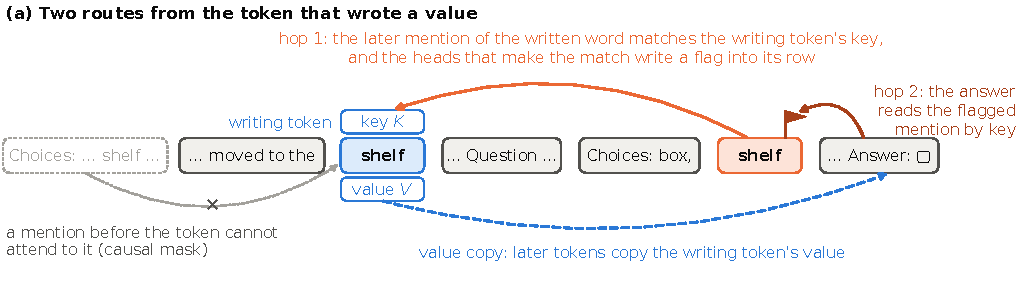
\includegraphics{figures/fig_schematic.pdf}}%
  \ifdim\ht2>160bp
    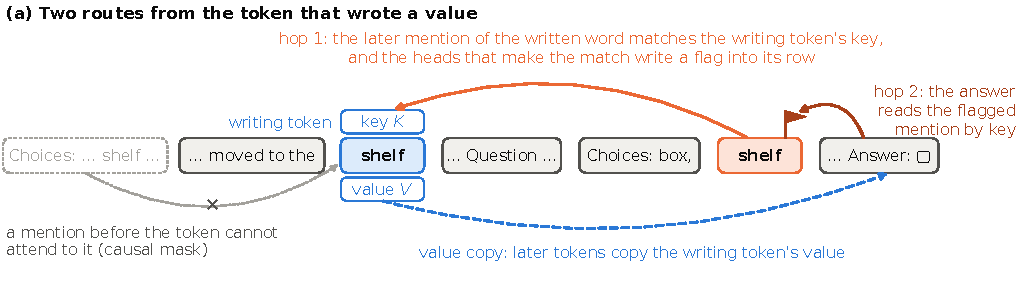
\includegraphics[width=\textwidth,trim=0 52 0 0,clip]{figures/fig_schematic.pdf}%
  \else
    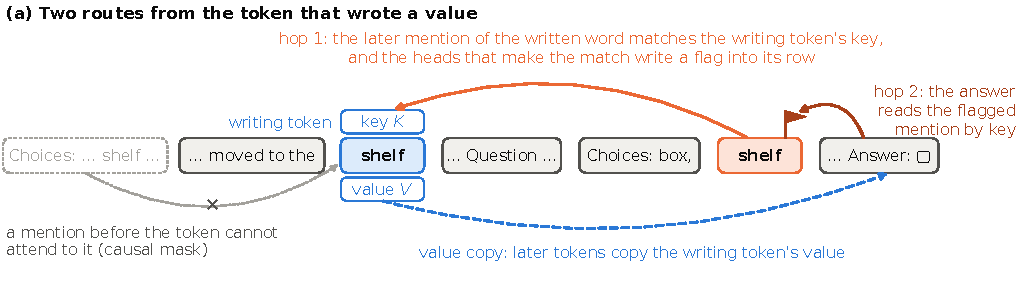
\includegraphics[width=\textwidth]{figures/fig_schematic.pdf}%
  \fi\\[2pt]
  % (b), (c): fig_fresh and fig_crossover_main carry their own panel tags. Until fig_crossover_main exists, the full
  % crossover figure is used with its zoom strip trimmed off, and both tags are set here, above the panels.
  \IfFileExists{figures/fig_crossover_main.pdf}{%
    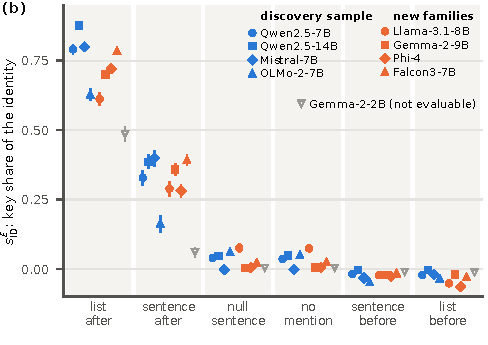
\includegraphics[width=0.49\textwidth]{figures/fig_fresh.pdf}\hfill
    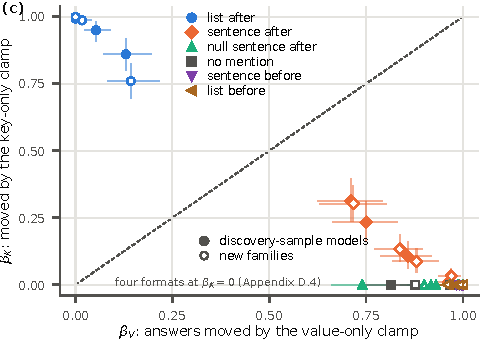
\includegraphics[width=0.49\textwidth]{figures/fig_crossover_main.pdf}%
  }{%
    \sbox2{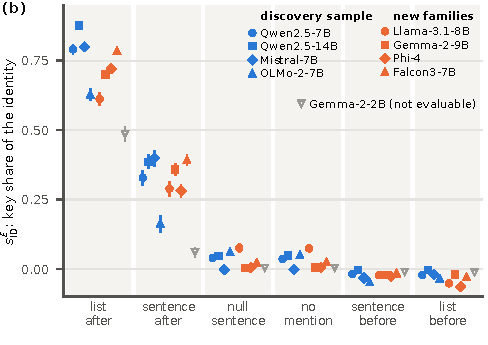
\includegraphics[width=0.49\textwidth]{figures/fig_fresh.pdf}}%
    \leavevmode\rlap{\raisebox{\ht2}{\sffamily\bfseries\scriptsize(b)}}\usebox2\hfill
    \sbox2{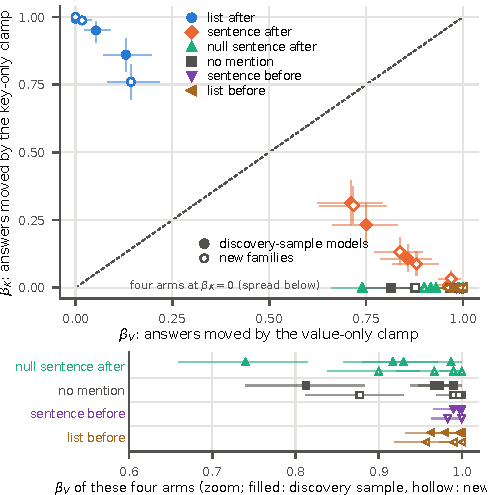
\includegraphics[width=0.49\textwidth,trim=0 70 0 0,clip]{figures/fig_crossover.pdf}}%
    \rlap{\raisebox{\ht2}{\sffamily\bfseries\scriptsize(c)}}\usebox2%
  }
  \caption{\textbf{Later mentions decide whether a written value is looked up through its key or copied from its value.} (a)~The writing token \emph{shelf} leaves a key $K$ and a value $V$ in the cache at every layer. A later mention of a candidate matches $K$ through heads with a duplicate-token core, which write a flag into the mention's row (hop~1; \cref{sec:claim2}); the answer reads the flagged mention by key (hop~2). Without a later mention the identity reaches the answer in $V$. We clamp $K$ and $V$ separately to another run's. (b)~Fresh stories, eight models: the key share of the value's identity, $s_{\mathrm{ID}}$, by where the candidates are named; emitted-form score; 95\,\% two-stage cluster intervals (98.75\,\% for the new families); grey: Gemma-2-2B, not evaluable. (c)~Generated answers: share moved to the clamped value by the key-only clamp ($\beta_K$) against the value-only clamp ($\beta_V$), per format and model; the four formats at zero key flips are spread out in \cref{app:generated}.}
  \label{fig:schematic}
\end{figure*}

\begin{table*}[t]
  \centering
  \caption{\textbf{What the architecture implies, what known circuits supply, and what we find.} ``Architecture alone'': what QK/OV and the causal mask imply \citep{elhage2021framework}. Unmarked findings were preregistered and held; ``risky'' marks predictions given a probability below 0.8 before the run. Every prediction, its prior and its verdict: \cref{app:prereg}.}
  \label{tab:qkov}
  \footnotesize\setlength{\tabcolsep}{3pt}
  \begin{tabular}{@{}p{0.17\textwidth}p{0.11\textwidth}p{0.21\textwidth}p{0.47\textwidth}@{}}
    \toprule
    Question & Architecture alone & Known circuits & What we find (status; section) \\
    \midrule
    \raggedright Can a mention \emph{before} the writing token read its key? & \raggedright No (causal mask) & \raggedright Options before a context cannot attend to it \citep{ok2026lost} & Nor does a later token read the key through it, in all eight story models and on passages; a list before even lowers the read below no mention (risky; held; unexplained) (\S\ref{sec:fresh}) \\
    \raggedright With the candidates named after it, is the value looked up or copied? & \raggedright Either: the copy route stays open & \raggedright Duplicate-token and induction heads attend to earlier copies \citep{wang2022ioi,olsson2022context} & Looked up: the key carries most of the identity in all eight story models ($s_{\mathrm{ID}}$ \JbRangeSidAfterNfourMin--\JbRangeSidAfterNfourMax{} in the new families) and in three evaluable passage models; copied without a later mention (\S\ref{sec:claim1}) \\
    \raggedright Must the later mention be an answer list? & \raggedright Not decided & \raggedright -- & Stories: a neutral sentence opens part of the read ($r$ = \JbRangeRPostNfourMin--\JbRangeRPostNfourMax{} in the new families; risky; held), a null sentence none; passages: only a small read (risky; did not hold) (\S\ref{sec:claim1}) \\
    \raggedright Does the route decide generated answers? & \raggedright Not decided & \raggedright -- & Stories: yes in all eight models, the sentence read in seven of eight; passages: with lettered options (risky; held), not with options by name or in free form (risky; did not hold) (\S\ref{sec:claim1}) \\
    \raggedright What does the matching head write? & \raggedright Not decided & \raggedright Binding ID vectors attached to entities \citep{feng2023binding} & A flag naming no candidate that moves the answer when injected and is read by key (risky; held); not specific, not necessary as one direction (risky; did not hold) (\S\ref{sec:claim2}) \\
    \raggedright What sets the sign of a key read? & \raggedright Not decided & \raggedright S-inhibition \citep{wang2022ioi}; copy suppression \citep{mcdougall2023copy} & The question, through the same readers; in IOI the key read is negative and the value read positive, applied at the names' keys (risky; held), not by the answer-side heads ranked in lists (risky; did not hold) (\S\ref{sec:claim2}) \\
    \raggedright Is an intervention's apparent channel a property of the edit? & \raggedright Not decided & \raggedright Steering via OV \citep{cheng2026steering}; keys as routers \citep{ma2025addressbook} & No: a released remap's channel flips with the format (discovery sample); the law that edits keep the model's own key-to-value ratio failed, even for near-natural steering vectors (did not hold) (\S\ref{sec:claim3}) \\
    \bottomrule
  \end{tabular}
\end{table*}

Mechanistic accounts often credit one cache channel: keys act as routers \citep{ma2025addressbook}, Llama models carry binding information mainly in key vectors \citep{oh2026rebinding}, an operation's cache is read mainly as an address \citep{wu2026record}, and refusal steering acts mainly through the OV circuit \citep{cheng2026steering}. Later tokens see a token only through its cached key and value, so a written value can reach the answer in two ways (\cref{fig:schematic}a). It is \emph{looked up} when a later token that already holds a candidate matches the writing token's key, so that the key itself carries which value was written; it is \emph{copied} when the identity travels in the writing token's value. What decides which route a model takes, and what follows for interventions that are credited to one channel?

In the belief stories of \citet{anonymous2026fitted}, one token, which they call the critical token and we call the \emph{writing token}, states where an object was moved. We clamp its cached key and value separately to another run's (clamping both from the first layer reproduces that run exactly; \cref{sec:method}) and vary only whether and where the candidates are named again: in \nModels{} discovery-sample models from three families (1.5B--72B), in a preregistered confirmation on 150 new stories in eight models from seven families (four never examined before), scored on emitted forms, and on counterfactual reading-comprehension passages with multi-token answers in four families. Before any output of the final round we recorded, for each of its \JxLinesABCD{} predictions, a probability of holding, a risk class and the text the paper would print for each outcome; we name every failure. From \citet{anonymous2026fitted} we take only the story template and, in \cref{sec:claim3}, one released remap and its training code; every other edit is built from public material.

\textbf{Later mentions decide the route} (\cref{sec:claim1}). With the candidates listed after the story, the writing token's key carries most of the value's identity in all eight confirmation models, and clamping only the key changes \pctn{\JbRangeBetaKAfterEightMin}--\pct{\JbRangeBetaKAfterEightMax} of generated answers to the clamped value; without a later mention the value carries the identity, and clamping only the value changes the answers (\cref{fig:schematic}b,c). A neutral sentence naming the candidates opens part of the key read, a length-matched one naming none opens nothing, and a list or sentence before the writing token opens none. On passages a later options list opens the key read too; that the channel decides the answer there we could show only for lettered options.

\textbf{A match at the later mention, read by key} (\cref{sec:claim2}). In two 7B models, heads with a duplicate-token core match the writing token's key at each later mention and write there a flag that names no candidate. Injected alone into the row of an option absent from the story, the flag moves the answer there and is read by key; but structured controls also move the answer, and removing the flag's direction leaves about half of the key read: sufficient, but neither specific nor necessary as one direction. Asked which option was \emph{not} mentioned, the same reader heads carry a negative read.

\textbf{Where an intervention appears to act} (\cref{sec:claim3}). In the discovery sample, a released learned remap \citep{anonymous2026fitted} has nearly the same behavioural effect in every format, yet the channel that appears to carry it flips from the keys with lettered options to the values without a later mention. A preregistered law predicting such attributions from the model's own key-to-value ratio failed: even near-natural steering vectors depart from it in some cells beyond the shallowest depth, and a remap trained at the writing token is read mainly through its value. Post hoc, departures grow with the edit's distance from the natural write.

\paragraph{What the architecture implies, and what it does not.}
Every attention head factors into a QK circuit, which decides where it attends, and an OV circuit, which decides what it moves \citep{elhage2021framework}. With the causal mask, a writing token's key can tell which value was written only to a later token that already holds a candidate, so a mention placed before it cannot read the key \citep[cf.][]{ok2026lost}. Duplicate-token and induction heads attend from later tokens to earlier copies \citep{wang2022ioi,olsson2022context}, option selection resembles query--key alignment \citep{tulchinskii2024wise}, and bound entities are retrieved through binding and ordering IDs, positions, lookbacks or a mix of these \citep{feng2023binding,dai2024binding,prakash2024finetuning,prakash2025lookbacks,gurarieh2025mixing}. None of this says which route a model takes, because the copy route is always open: the answer can attend to the writing token and copy its value. We find, each by a preregistered test, what the architecture allows but does not imply (\cref{tab:qkov}): the tokens after the writing token choose the route, in every family we tested and in generated answers; after an earlier list no later token looks the key up; the match writes a flag that names no candidate, sufficient to move the answer and read by key, though neither specific nor necessary as one direction; and the key read can take the opposite sign of the value read (\cref{sec:claim2}). We claim no new head type.

\section{Setup}\label{sec:method}

\paragraph{Stories, runs and formats.}
We use the belief stories of \citet{anonymous2026fitted} (``[\dots] \{agent\} watches as the \{$o$\} is moved to the \{\textsc{loc}\}. [\dots] Where does \{agent\} believe the \{$o$\} is?''; \cref{app:prompts}). Base and source stories B and S differ only at the writing token \{\textsc{loc}\}, at position $p$; a third value X is absent from the story. \fmtOpt{} lists the candidates after the question (``Answer with exactly one choice''), \fmtLetter{} labels them A--F; under ``Answer with one word'', \fmtListA{} lists them there, \fmtPost{} names them in a neutral sentence after the story, \fmtNull{} replaces it by one of the same length that names none, \fmtSentB{} and \fmtBefore{} put the sentence or the list before the story, and \fmtNone{} names none. A \emph{later mention} is a token after $p$ that repeats a candidate's word form, up to case: a synonym or a word of another language in its place opens at most \GfifteenRKMax{} of an exact repeat's key read on our English-scored measure (discovery sample; \cref{app:readers}). The \emph{fresh stories} are 150 new cores of the same template, with eight new mention sentences, a second location lexicon and per-core candidate orders (\cref{app:fresh}).

\paragraph{Passages.}
From the SQuAD v1.1 development set \citep{rajpurkar2016squad} we take questions whose answer is a person, place or number named exactly once in the passage, with no content word of it elsewhere, and write a counterfactual entity in its place \citep{longpre2021conflicts}: 185 items from 34 articles, with answers of one to five tokens, clamped at every position of the span. Formats: options after the question (by name or letter) or before the passage, a related-articles sentence after or before it, or free form. We score the first answer token (\cref{app:natural}).

\paragraph{Clamps.}
$\mathcal{C}_K(Z)$ sets the writing token's pre-RoPE key in every layer from $\ell_0$ ($0$ unless stated) to that of run $Z$, and $\mathcal{C}_V(Z)$ its value. Later tokens see the writing token only through these, so clamping both from layer~0 reproduces run $Z$ exactly (checked in FP32; \cref{app:impl}). A single-channel clamp creates a cache state that no prompt produces; generated answers under it show that the read reaches behaviour, not that the state is natural.

\paragraph{Measures.}
With $\Delta_Y(Z)$ the change in $\log p(Y)$ at the answer under $\mathcal{C}_K(Z)$ against a self-clamp row in the same batch,
\begin{equation}\label{eq:idk}
\mathrm{ID}_K = \tfrac{1}{2}\big[\Delta_{\mathrm{S}}(\mathrm{S}) - \Delta_{\mathrm{S}}(\mathrm{X}) + \Delta_{\mathrm{X}}(\mathrm{X}) - \Delta_{\mathrm{X}}(\mathrm{S})\big],
\end{equation}
that is, how much more a key clamp to S favours S over X than a clamp to X does, averaged symmetrically; effects shared by all foreign keys, and a prior for B, cancel, and it is zero when the key carries no identity. $\mathrm{ID}_V$ is defined likewise with values, $s_{\mathrm{ID}} = \overline{\mathrm{ID}}_K/(\overline{\mathrm{ID}}_K + \overline{\mathrm{ID}}_V)$ is a ratio of means, and $r$ is a format's $\overline{\mathrm{ID}}_K$ relative to that with the list after the story. Under the \emph{emitted-form score}, a candidate's probability is summed over the surface forms the model itself emits on held-out stories (\cref{app:emitted}); the discovery sample keeps its lower-case score (the probability of the lower-case word after a space). Under each clamp we also decode greedily: $\beta_K$ ($\beta_V$) is the share of answers that move to the clamped value under the key-only (value-only) clamp, net of moves to it under the clamp to the other of S and X; the flip rate omits that correction.

\paragraph{Models and statistics.}
The discovery sample has \nModels{} models: Qwen2.5 at 1.5B--72B \citep{yang2024qwen25}, Qwen3-8B \citep{yang2025qwen3}, Mistral-7B \citep{jiang2023mistral}, Mistral-Small-24B \citep{mistral2025small} and OLMo-2-7B \citep{olmo2025two}; the final round adds Llama-3.1-8B \citep{grattafiori2024llama3}, Gemma-2-9B and Gemma-2-2B \citep{gemma2024gemma2}, Phi-4 \citep{abdin2024phi4} and Falcon3-7B \citep{tii2024falcon3}. All are instruction-tuned and run in BF16, those of the final round from official weights (sha256-verified; \cref{app:compute}). Intervals are 95\,\% percentile bootstrap intervals, two-stage over clusters on fresh stories and passages, and in the mechanism tests over stories with the flag's fit fixed (so they exclude its uncertainty); the intervention law uses 90\,\% intervals (two one-sided tests; \cref{app:lawresults}). A prediction over several models must hold in every evaluable model, one over the four new families in three of them (98.75\,\% intervals). Holm's step-down over each part's risky interval components changes no verdict (\cref{app:prereg-j}).

\paragraph{Preregistration and status marks.}
Each of ten preregistrations was committed before its run, with its scoring code fixed before any output was inspected. Each prediction of the final round had a recorded probability of holding: a \emph{replication} at least 0.9 (implied by data in hand), an \emph{extrapolation} at least 0.8, a \emph{risky} prediction less. Where two rules of the entry conflicted (the title's scope, one evaluability rule), we followed the more specific one; both choices favour our account (\cref{app:decisions}). Unless marked, a result in \cref{sec:claim1,sec:claim2,sec:claim3} was preregistered in the final round and held; \rsk{} marks a risky prediction, failures are said in words, other results are labelled discovery sample, exploratory or post hoc, and \cref{app:crosswalk} maps each sentence to its prediction.

\begin{figure*}[t]
  \centering
  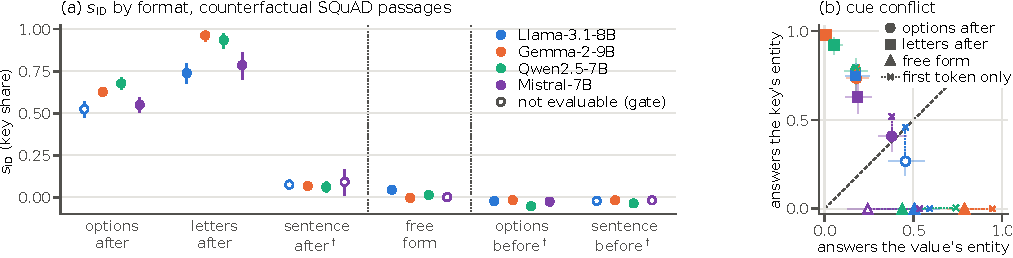
\includegraphics[width=\textwidth]{figures/fig_natural.pdf}
  \caption{\textbf{On passages, a later options list makes the model read the answer entity's identity through its cached keys; with lettered options, generated answers follow the key's entity in all four models.} Counterfactual SQuAD passages, four models, 185 items; 95\,\% two-stage article-cluster intervals. (a)~$s_{\mathrm{ID}}$ by format, at the first answer token; hollow: not evaluable (preregistered gate); $\dagger$: recomputed (exploratory). (b)~Cue conflict (key and value from two counterfactual entities): share of answers naming the key's or the value's entity; crosses: decision token alone; a boundary, not a confirmed claim.}
  \label{fig:natural}
\end{figure*}

\section{Later mentions decide whether a value is looked up or copied}\label{sec:claim1}

\textbf{When the candidates are named again after the writing token, later tokens read its key and the value's identity is looked up; without such a mention it is copied from the value.} Position decides, with the instruction held fixed, and the decision reaches generated answers. We call this the \emph{format law}.

\subsection{Fresh stories in seven families}\label{sec:fresh}

In the discovery sample (\cref{app:discovery}) a list after the story opened a large key read, also on two further tasks, an instruction-matched $2{\times}2$ showed that position decides, and the channels carried which value was written, not its belief role.\label{sec:scope} The confirmation ran on the 150 fresh stories in four discovery-sample models (Qwen2.5-7B and 14B, Mistral-7B, OLMo-2-7B) and four new families (\cref{fig:schematic}b). In four model families never examined before, a list of the candidates after the story makes the writing token's key carry most of the value's identity ($s_{\mathrm{ID}} \geq 0.5$ in \JbOneNfMet{} of \JbOneNfEval{}), as in the four discovery-sample models ($s_{\mathrm{ID}}$ \JbRangeSidAfterEightMin--\JbRangeSidAfterEightMax{} over all eight). Without a later mention, the identity is copied through the value in every family ($s_{\mathrm{ID}} \leq 0.1$ under \fmtNone{}). The same list or sentence before the story opens no key read in any model; in the four new families a list before even lowers the key read below its no-mention level\rsk, which we do not explain (\cref{sec:limitations}).

A neutral sentence naming the candidates after the story opens an intermediate key read ($r$ = \JbRangeRPostNfourMin--\JbRangeRPostNfourMax{} of the list read) in \JbThreeNfMet{} of \JbThreeNfEval{} new families\rsk, as in the four discovery-sample models. A sentence of the same length naming no candidate opens no key read, so the read needs the re-mention (\rsk{} in the new families); in Llama-3.1-8B it missed its threshold through a small key read without any mention ($r$ = \JbRNoneLlamaEight{}), to which the null sentence adds almost nothing (post hoc reading). At 2B (Gemma-2-2B) the prediction\rsk{} of almost no sentence read was not evaluable: the model failed the competence gate, answering too few clean stories correctly (had it passed, the prediction would not have held; post hoc; \cref{app:fresh}).

\paragraph{Generated answers.}
Clamping only the writing token's key changes the generated answer to the clamped value in \pctn{\JbRangeBetaKAfterEightMin}--\pct{\JbRangeBetaKAfterEightMax} of stories when the candidates are listed after it and in at most \pct{\JbRangeBetaKNoneEightMax} when they are not; clamping only its value does the reverse (\cref{fig:schematic}c). (`Not': no mention, a list or a sentence before; without a mention the value-only clamp changes \pctn{\JbRangeBetaVNoneEightMin}--\pct{\JbRangeBetaVNoneEightMax}.) The sentence read changes generated answers\rsk{} in seven of the eight models (flip rate \pctn{\JbFivebFlipPostMetMin}--\pct{\JbFivebFlipPostMetMax} after the sentence, \pct{\JbRangeFlipPreEightMax} before it), a small share in most. This held in the new families; at OLMo-2-7B the read is visible in log-probabilities but not in generated answers (flip rate 1.0\,\% after, 0\,\% before), so in the discovery-sample models the prediction did not hold (we worded this split after the data; \cref{app:decisions}). % verbatim: outcome J part B

\paragraph{The measurement.}
Scored on the forms the models actually emit (coverage $\geq 0.8$ in every cell), every re-scored verdict on the original stories is unchanged\rsk. $s_{\mathrm{ID}}$ moves by at most 0.05, while the sentence read relative to the list read, $r$, rises under emitted forms by $+$\JbSixbRPostMistralSeven{} at Mistral-7B and by $+$\JbSixbRPostQwenFourteen{} at Qwen2.5-14B, where equivalence within 0.05 is not shown, so its predicted invariance did not hold\rsk: the lower-case score understated the sentence read. Two further validity checks held\rsk{} (\cref{app:measure}).

\subsection{Reading-comprehension passages}\label{sec:natural}

On counterfactual SQuAD passages, a later options list makes the model read the passage entity through its cached keys ($s_{\mathrm{ID}}$ \JaSidOptaMistralSeven--\JaSidOptaQwenSeven{} in Gemma-2-9B, Qwen2.5-7B and Mistral-7B), and without it through its values ($s_{\mathrm{ID}}$ at most \JaSidNomLlamaEight{} in Llama-3.1-8B, Gemma-2-9B and Qwen2.5-7B; \cref{fig:natural}a). The key read with options after holds for answers of three or more tokens\rsk{} and, with lettered options, in all four models. Two cells these claims use failed gates (\JaGateFailCells{} of 24 in all; \cref{app:natural}), so the derived within-model contrast was not evaluable (it held where computable); under one of two conflicting rules this would have restricted the title to templated stories (\cref{app:decisions}). Options before the passage leave a small negative key read. The prediction that a related-articles sentence after the passage opens the key read did not hold\rsk: it opens only a small key read ($s_{\mathrm{ID}}$ gain \JaFiveDiffQwenSeven--\JaFiveDiffGemmaNine{} in Gemma and Qwen, the evaluable models), so on passages our claim concerns a later options list.

\paragraph{Behaviour on passages is a boundary.}
In cue conflict (key and value from two counterfactual entities), with lettered options the generated answer follows the key's entity in all four models (key-source rate \JaKeySrcLetaMistralSeven--\JaKeySrcLetaGemmaNine)\rsk, though in Mistral-7B it passes Holm's correction only within Monte Carlo error. With options answered by name the prediction that the key wins did not hold\rsk: it wins in Gemma and Qwen, not in Mistral (Llama's cell is not evaluable), although a key that matches no option leaves the value to be copied\rsk. In free form the decision token follows the value while the continuation breaks (hybrids, an observation), so too few whole answers name the value's entity and that prediction did not hold\rsk{} either (\cref{fig:natural}b). The channel attributions are therefore not shown to decide behaviour on natural text. Two predictions on 2-bit quantization of the cached values and one on the rate of hybrids did not hold\rsk; the reader-head tests\rsk{} and three further passage tests (one risky) were not evaluable, because their gates failed (\cref{app:natural}).

% The stage-9 window figure of Section 5 (defined here so that it floats to the page where Section 5 starts)
\begin{figure*}[t]
  \centering
  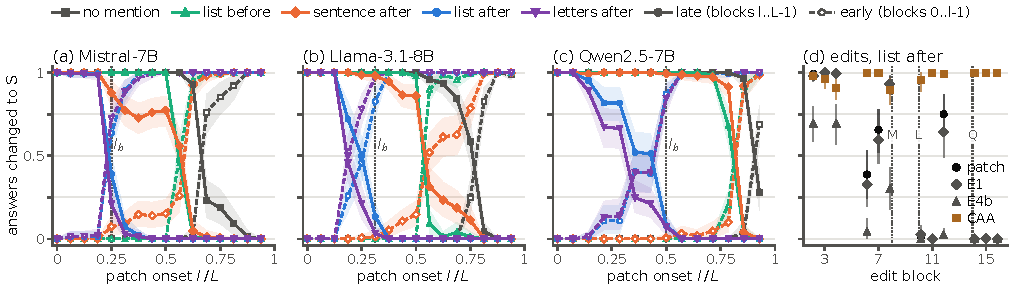
\includegraphics[width=\textwidth]{figures/fig_window.pdf}
  \caption{\textbf{With the candidates listed after the story, a patch of the writing token's cache must reach its early layers to change the answer.} Stage 9. (a--c)~Share of generated answers changed to S, the source story's value, by the late patch (S's key and value at the writing token from block $l$ to the top; solid) and by the early patch (below block $l$; dashed), against the onset $l$ as a fraction of the depth $L$, by format (\NqStories{} new stories; 95\,\% two-stage cluster intervals as bands); dotted: $l_b$, the first onset whose late patch changed at most 0.2 of \fmtListA{} answers on earlier stories. (d)~Share of \fmtListA{} answers changed by edits written at blocks 3--15: the natural patch, single-site steering (E1), the trained remap (E4b; not run at Llama) and steering at every position from the writing token on, generated tokens included (CAA); in each block, Mistral-7B, Llama-3.1-8B and Qwen2.5-7B from left to right; dotted: $l_b$ (M, L, Q: blocks \NqLbMistralSeven, \NqLbLlamaEight, \NqLbQwenSeven; \NqCores{} edit cores).}
  \label{fig:window}
\end{figure*}

\section{A match at the later mention, read by key}\label{sec:claim2}

\textbf{In two 7B models (Qwen2.5-7B, Mistral-7B), the reader heads match the writing token's key at the later mention of the written value and write a flag into that mention's row, which the answer reads by key.} The flag suffices to move the answer but is neither specific nor the only carrier, and the question sets the sign of the read (details in \cref{app:claim2-brief}, \cref{fig:flag}).

\paragraph{Two hops.}
In the discovery sample, 5\,\% of heads, the \emph{reader heads}, read the writing token's key at the option words (hop~1): seeing the clamped key alone, they recover \HoneRQwenSeven{} and \HoneRMistralSeven{} of the option rows' read (\cref{app:heads}). They are enriched for duplicate-token heads \citep{wang2022ioi} (exploratory). Mean-ablating them at the option rows leaves \HthreeRhoQwenSeven{} and \HthreeRhoMistralSeven{} of the key read and raises the value read: a copy route stays available. The answer reads the option words, not the writing token (hop~2), mainly by key, so in lists the written value is read at its later mention, not looked back for at the token that states it.

\paragraph{What the readers write.}
The reader heads write one vector per layer into the re-mentioned word's row. We call it the \emph{flag}. Injected with no key clamp into the row of an option absent from the story, a version fit without that word moves the answer there (\JdOneRatioQwenSeven{} / \JdOneRatioMistralSeven{} of the key read's identity effect; the answer changes in \pct{\JdOnePiXQwenSeven} / \pct{\JdOnePiXMistralSeven} of stories)\rsk; like the natural key clamp, the injection adds the flag at that row and removes it at the base value's row. Its mean direction names no candidate. The answer reads it by key, as it reads the natural one (giving only the answer row the option rows' original keys removes \JdFourKQwenSeven{} / \JdFourKMistralSeven{} of its effect). But the prediction\rsk{} that it is specific failed against structured controls, and one direction per layer does not carry the key read ($\rho_K$ = \JdThreeRhoFlagQwenSeven{} / \JdThreeRhoFlagMistralSeven{}): other carriers exist; the flag is sufficient but not necessary. Removing it leaves about half of the key read, as the prediction\rsk{} allowed, but the line failed on its control directions, which overlap the flag (\cref{app:decisions}). % verbatim: outcome J part D

\paragraph{The sign of the read.}
Asked which option was \emph{not} mentioned, both reads turn negative and the same reader heads carry them; that the sign is applied after the first hop is exploratory. In indirect-object identification (IOI) with the names re-mentioned in a parenthesis, the key read is negative and the value read positive in both models, consistent with S-inhibition \citep{wang2022ioi}, and the negative read is applied where the answer reads the listed names, more by key than by value (restoring their keys and values for the answer row alone removes \JdRouteKVQwenSeven{} / \JdRouteKVMistralSeven{} of it)\rsk. The prediction\rsk{} that the ten answer-side heads ranked in lists apply it failed: a different (or a distributed) reader applies the negative read. That the belief readers carry the IOI read\rsk{} was met at Qwen2.5-7B and is not evaluable at Mistral-7B. The flag is written in sentences as in lists at 1.5B--7B, but four further predictions\rsk{} did not hold: that it carries the size of the sentence read across scale and is read by value at 1.5B (the decision table gives ``Mixed.''), that the initial-state flag carries binding separably from order, and that a key naming no candidate acts as removing the base value's flag (\cref{app:sign,app:scale}).

\section{Where an intervention appears to act}\label{sec:claim3}

\begin{figure*}[t]
  \centering
  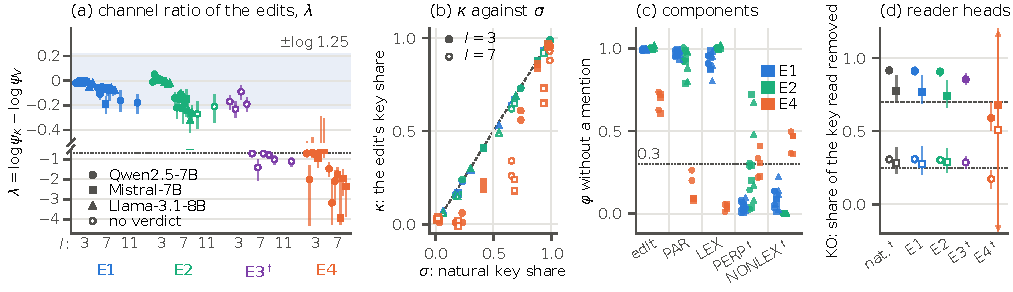
\includegraphics[width=\textwidth]{figures/fig_law.pdf}
  \caption{\textbf{The preregistered channel-ratio law failed.} Qwen2.5-7B, Mistral-7B and Llama-3.1-8B, 80 stories. (a)~$\lambda = \log\psi_K - \log\psi_V$ per edit family (E1, E2: steering vectors from held-out stories and from unrelated sentences; E3: features of a public sparse autoencoder; E4: a remap trained at the writing token), depth and format, with 90\,\% intervals and the $\pm\log 1.25$ band; hollow: no verdict (E3's gate failed; values recomputed). (b)~$\kappa$, the edit's key share, against $\sigma$, the natural key share at the same depth and format (descriptive). (c)~Identity effect without a mention of each edit's component along the natural write (PAR), along the English lexical span (LEX) and orthogonal to each. (d)~Share of the key read removed by blocking the reader heads, per family, beside the natural write; open: random head sets, which the natural write also fails to keep under the preregistered 0.25.}
  \label{fig:law}
\end{figure*}

\textbf{Which cache channel an intervention appears to act through depends on the prompt and on the edit; a preregistered law that would have predicted it from the model's own read failed.}

\paragraph{A motivating case.}
The released remap of \citet{anonymous2026fitted} is a rank-16 distributed alignment search subspace \citep{geiger2024finding} at the output of block 4 over the move event, trained so that the model answers a fixed permutation of the source location. With \fmtOpt{}, a key-only exchange at the writing token attributes part of its effect, beyond a PCA control, to the keys, as we reproduce (\cref{app:remap}). Changing only the format barely changes its behavioural effect, yet the channel that appears to carry it flips: at Qwen2.5-72B its keys carry \psiLetterQwen{} of the effect with lettered options and \psiNoneQwen{} without a later mention, its values the reverse (discovery sample; likewise for a refit without later mentions).

\paragraph{The law and its test.}
We preregistered a law that extends the \emph{format law} of \cref{sec:claim1} from the model's own read to edits: an edit written at the writing token at depth $l$ is read through key and value in the model's own ratio at that depth and format. With $\psi_C$ the edit's identity effect through channel $C$ as a share of the natural write's, from block $l{+}1$ on,
\begin{equation}\label{eq:lambda}
\lambda = \log\left(\psi_K/\psi_V\right),
\end{equation}
and the law holds in a cell when the 90\,\% interval of $\lambda$ lies inside $\pm\log 1.25$. An edit at the writing token reaches later tokens only through its keys and values, and as the runs differ only there, writing the source run's residual is the natural clamp itself: our equivalence control. Rows with the key moved halfway were classified as departures (\cref{app:law}). Five families were tested, in up to three models, four depths and four formats: steering vectors from held-out stories or unrelated sentences \citep{turner2023actadd,panickssery2023caa}; features of a public sparse autoencoder \citep{bussmann2024batchtopk,andyrdt2025saes}; a rank-16 remap trained at the writing token with the released training code of \citet{anonymous2026fitted}; and \emph{non-lexical} steering vectors, which write the value in another language, as a synonym, or without its English lexical component (\cref{app:edits}).

\paragraph{The outcome.}
Even steering vectors close to the natural edit depart from the natural channel ratio; the format law describes the model's own written value and does not predict how an edit is attributed. In the preregistered core test the steering vectors' departures are small but graded ($\bar\lambda$ = $\JcOnePoolEoneMistralSeven$ to $\JcOnePoolEtwoMistralSeven$; every pooled value inside the margin, not every statistic): the format law does not transfer to edits as a channel-ratio law (did not hold; in Llama-3.1-8B for the vectors from unrelated sentences too; \cref{fig:law}a,~b). At the shallowest depth every statistic is equivalent ($|\lambda| \leq \JcOneLamThreeAbsMax$; exploratory); deeper, the keys under-read the steering vectors, pooled by 4.5--12\,\% ($\bar\lambda$ $\JcTwoPoolEoneLlamaEight$ to $\JcTwoPoolEtwoLlamaEight$), % verbatim: outcome J part C
and every failing statistic sits in a cell with a small natural key read (\JcOneNeIDKMin--\JcOneNeIDKMax{} nats; post hoc).

\paragraph{Edits far from the natural write.}
Edits that change the value through a learned remap are read mainly through the value ($\bar\lambda$ = $\JcFourPoolEfourQwenSeven$ / $\JcFourPoolEfourMistralSeven$): the key channel does not read them as it reads the written word (risky; did not hold). Its size depends on depth (under \fmtPost{} at block 7, $\psi_K$ \JcFourPsiKWpostSevenQwenSeven{} against $\psi_V$ \JcFourPsiVWpostSevenQwenSeven{} at Qwen2.5-7B; post hoc). The autoencoder test was not evaluable: its gate scored positions that the dictionary's published fit excludes. Identity-carrying components orthogonal to the natural write or to the lexical span are also read mainly through the value (risky; did not hold; \cref{fig:law}c). The non-lexical steering vectors are read less through the key, but write far from the natural state: the predicted lexical boundary was not isolated, so we claim neither that the token-form account holds for edits nor that it is contradicted (risky; did not hold). The reader heads read the steering vectors like the natural value, but the test failed on a random-set control that the natural value also fails (did not hold; post hoc reading), and it was not evaluable for the autoencoder and the remap (failed gate; small key read; \cref{fig:law}d, \cref{app:lawresults}).

\paragraph{Post hoc: distance from the natural write.}
Post hoc, the departures follow how far an edit's cached keys and values lie from the natural ones ($\nu$, a relative distance): of the $\lambda$ statistics of identity-carrying edits, \JcNuEqLow{} of \JcNuNLow{} with $\nu < 0.1$ are equivalent, \JcNuEqMid{} of \JcNuNMid{} with $\nu$ between 0.1 and 0.3, and \JcNuEqHigh{} of \JcNuNHigh{} beyond (Spearman $\JcNuRhoNu$; \cref{app:nu}). $\nu$ is collinear with the key cosine, so which matters is open. Rule: report an intervention's channel only beside the model's own read at the same depth, in more than one prompt, and with the edit's distance from the natural write.

\paragraph{The binding swap of \citet{prakash2025lookbacks}.}
At block 28 of Qwen2.5-14B an identity edit is copy-read like the natural value ($\kappa \leq 0.30$), while the binding swap there is key-read; key-flat reading is not a property of depth for identity edits ($\kappa$ \JcSixKappaCaaNoMention{} against \JcSixKappaBindNoMention{} without a mention). This does not separate kind from depth, because the natural read there is itself copy-only, and the swap changes no answer in two of the three formats. Binding forms only after the identity key route closes in every model screened, so a binding swap cannot be compared with an identity edit at a depth where the key route is open (risky; held; a prediction for such a window was not evaluable); the four earlier preregistered predictions on this swap, which failed, stand (\cref{app:binding}).

\section{Related Work}\label{sec:related}

\paragraph{Options, belief stories and heads.}
Specific heads select among listed options \citep{lieberum2023chinchilla,wiegreffe2025answer}, select-and-copy heads by query--key alignment \citep{tulchinskii2024wise}; our second hop, in which the answer selects the flagged option rows by key, resembles this selection. Closest to our first hop, shallower heads write into option rows a one-dimensional option-routing feature that redirects the attention of decision heads \citep{sun2026persuaded}; our flag plays this role, written by a duplicate-token match to the token that wrote the value, with a mean direction that is the same whichever value was written. On belief stories, belief and reality share a value slot read out under a router at the query \citep{steele2026routing}, and lookbacks built on ordering IDs track beliefs \citep{prakash2025lookbacks}; in our terms both describe a copy route from the token that states the value, and later mentions add a second route, addressed at the mention.

\paragraph{Attributing interventions.}
Interchange interventions \citep{geiger2021inducing,geiger2024finding} may act through pathways the model does not use naturally (\citealp{makelov2024subspace,liu2026wrong}; contested by \citealp{wu2024reply}); steering vectors \citep{turner2023actadd,panickssery2023caa} need not reproduce natural activations \citep{shih2026steering} and are brittle to prompt changes \citep{tan2024steering}. Prompt format changes what is measured \citep{sclar2023quantifying,opielka2026causality}, and the answer encoding under which a steering gain is measured changes what it identifies \citep{gao2026encodings}; we find the same for the cache channel through which an edit appears to act. Cache-level accounts place routing or binding information in keys \citep{ma2025addressbook,oh2026rebinding} or find an operation's cache read mainly as an address \citep{wu2026record}; in our stories the token that wrote a value is read mainly through its key only when a later token re-mentions the candidates.

\section{Discussion}\label{sec:discussion}

\begin{table}[t]
  \centering
  \caption{\textbf{How the predictions of the final preregistration fared.} Held / with a verdict (expected: sum of the recorded probabilities); n.e.: not evaluable, not counted.}
  \label{tab:status}
  \scriptsize\setlength{\tabcolsep}{2.5pt}
  \IfFileExists{tables/tab_status.tex}{\input{tables/tab_status.tex}}{%
  % The cells from the class macros; "with a verdict" = met + not met, summed by TeX from the printed counts; expected in brackets.
  \begin{tabular}{@{}lcccc@{}}
    \toprule
    Evidence (claim) & Replication & Extrapolation & Risky & n.e. \\
    \midrule
    Fresh stories (1) & \JbClassLMet/\the\numexpr\JbClassLMet+\JbClassLNotMet\relax{} (\JbClassLExp) & \JbClassMMet/\the\numexpr\JbClassMMet+\JbClassMNotMet\relax{} (\JbClassMExp) & \JxRiskyMetB/\JxRiskyVerdB{} (\JxRiskyExpB) & \JbCountNotEval \\
    Passages (1) & \JaClassLMet/\the\numexpr\JaClassLMet+\JaClassLNotMet\relax{} (\JaClassLExp) & \JaClassMMet/\the\numexpr\JaClassMMet+\JaClassMNotMet\relax{} (\JaClassMExp) & \JxRiskyMetA/\JxRiskyVerdA{} (\JxRiskyExpA) & \JaCountNotEval \\
    Mechanism (2) & \JdClassLMet/\the\numexpr\JdClassLMet+\JdClassLNotMet\relax{} (\JdClassLExp) & \JdClassMMet/\the\numexpr\JdClassMMet+\JdClassMNotMet\relax{} (\JdClassMExp) & \JxRiskyMetD/\JxRiskyVerdD{} (\JxRiskyExpD) & \JdCountNotEval \\
    Interventions (3) & -- & \JcClassMMet/\the\numexpr\JcClassMMet+\JcClassMNotMet\relax{} (\JcClassMExp) & \JxRiskyMetC/\JxRiskyVerdC{} (\JxRiskyExpC) & \JcCountNotEval \\
    \midrule
    All & \JxClassLMetABCD/\JxClassLVerdABCD{} (\JxClassLExpABCD) & \JxClassMMetABCD/\JxClassMVerdABCD{} (\JxClassMExpABCD) & \JxRiskyMetABCD/\JxRiskyVerdABCD{} (\JxRiskyExpABCD) & \JxNotEvalABCD \\
    \midrule
    \multicolumn{3}{@{}l}{Measurement validity (fresh stories)} & \JxClassValMetABCD/\JxClassValVerdABCD{} (\JxClassValExpABCD) & \JbClassValNotEval \\
    \bottomrule
  \end{tabular}}
\end{table}

\paragraph{What to do differently.}
(i)~State where the candidates are mentioned relative to the token that writes a value, and test channel claims with and without a later mention. (ii)~Check localisation methods \citep{mueller2025mib} in the format of the behaviour they should explain. (iii)~Measure an intervention's channels with key-only and value-only exchanges rather than infer them from the model's own read, and report the edit's distance from the natural state (post hoc here): beyond the shallowest depth even near-natural steering vectors were under-read by the keys (exploratory), and the remap we trained far more. (iv)~Do not credit a context token from the answer's attention alone: with the candidates listed after the story, cutting the answer's attention to the writing token leaves the answer intact, while without a mention it removes most of the models' ability to answer (discovery sample; \cref{app:g-knockout}). (v)~When patching attention, disable the KV cache and keep one attention kernel (\cref{app:impl}).

\paragraph{How the predictions fared.}
The risky predictions (\cref{tab:status}) held \JxRiskyMetABCD{} of \JxRiskyVerdABCD{} against \JxRiskyExpABCD{} expected, within chance under the recorded priors (probability \JxRiskyTailP{} of so few or fewer if independent; post hoc), and \JxRiskyMetABCDAlt{} of \JxRiskyVerdABCDAlt{} (expected \JxRiskyExpABCDAlt{}) under the stricter of two conflicting evaluability rules. Of the \JxRiskyNotEvalABCD{} risky predictions not evaluable, \JxRiskySensNotHeld{} would not have held, \JxRiskySensHeld{} would have and one is unresolved: \JxRiskySensMet{} of \JxRiskySensVerd{} (expected \JxRiskySensExp{}; post hoc; \cref{app:prereg-j}). The extrapolations all held on claims 1 and 2 (probability \JxClassMTailPABD{} that all would) but \JcClassMMet{} of \JcClassMLines{} on the interventions (expected \JcClassMExp{}; probability \JcClassMTailP{} if independent, which overstates the evidence), the clearest shortfall among the class tallies (Brier score \JcClassMBrier), singled out after the data (post hoc). In entries G to I, \GHIcountFailed{} of \GHIcountVerd{} predictions with a verdict failed, and in A to F a transfer law for interventions (not the law of \cref{sec:claim3}) and a key-share threshold failed (\cref{app:prereg-ai}); every failure of the final round is listed in \cref{app:failures-j}.

\paragraph{Limitations.}\label{sec:limitations}
(i)~Our passages are counterfactual SQuAD items with added options and the answer named once, scored at the first answer token; naturally occurring later mentions, and passages in which the answer recurs with the counterfactual written at every mention, are the test we most lack. (ii)~The confirmation uses one story template. (iii)~A later mention here repeats the word form (plurals open \GfourteenPluralMin--\GfourteenPluralMax{} of the read; discovery sample); paraphrases and pronouns are untested. (iv)~A list before the writing token gives a small negative key read (to $\idKBeforeQwenSeventytwo$ nats at Qwen2.5-72B), as in IOI, perhaps a suppression of a word seen twice by heads we did not identify. (v)~From a clamp onset at 30\,\% of the depth, the key share stays at or above one half in seven of ten discovery-sample models, but on passages only \JaEoneOnOptaMin--\JaEoneOnOptaMax{} of the key read remains (exploratory; descriptive, as the effects no longer add). (vi)~The readers' duplicate-token core depends on how many heads are counted; ablation and knockout disagree on whether the copy route takes over; how the answer prefers the moved-to location over the initial one, also mentioned, is unresolved. (vii)~The mechanism was tested in two 7B models (and at 1.5B and 3B), the channel-ratio law in three 7--8B models, all in BF16; eager attention, which Gemma-2 requires, lowers the key read by 12--17\,\% in one model (exploratory), though no Gemma-2-9B verdict lies within 0.03 of its threshold; the list-after share falls beyond 14B for unknown reasons (discovery sample). % verbatim: "12 % (AFTER) and 17 % (POST)" and "no Gemma-2-9B verdict is within 0.03 of its threshold", outcome J part B
(viii)~Values span one to five tokens and prompts are English; the final round's models are instruction-tuned, and in the base models we ran on IOI a later list opened no positive key read (a weak null at Qwen2.5-7B base; discovery sample, exploratory; \cref{app:g-ioi}). (ix)~We re-tested no third-party channel claim with and without a later mention.

\paragraph{Conclusion.}
Across seven model families on fresh stories, and for an appended options list on counterfactual passages in every evaluable model, later mentions decide whether a written value is looked up through its key or copied from its value; on fresh stories the decision reaches generated answers. % seven = \JxFamiliesABCD (design count)
In two 7B models, the matching heads, enriched for duplicate-token heads (discovery sample), write a flag that the answer reads by key, sufficient but neither specific nor the only carrier. Where an intervention appears to act depends on the prompt and the edit; a preregistered law predicting it from the model's own read failed.

\section*{Impact Statement}
This work aims to make explanations of language-model internals more reliable, by showing that the cache channel that appears to carry a value or an intervention depends on the prompt under which it is measured. More reliable component-level explanations could help researchers audit and debug models, and could reduce the risk that a mechanism found under one evaluation format is trusted to explain behaviour under another. Our results also caution against over-reading interpretability findings: an attribution validated under one prompt format, or inferred from the model's own read, should not on its own certify behaviour under others. Methods for locating and editing what a model reads from its context could also be used to steer models in unwanted ways; our experiments use public models, templated stories, public reading-comprehension passages, edits built from public material, a released remap and a released state-token patch.


\bibliography{references}
\bibliographystyle{icml2026}

\newpage
\appendix
\onecolumn
% Appendix wrapper. main.tex issues \appendix and \onecolumn before \input'ing this file.
% A: preregistrations and claim status; B: prompts and items; C: implementation; D--F: details of Claims 1--3;
% G: the released remap; H: the binding swap; I: competing accounts and further related work; J: models and compute.
\section*{Reader's guide to the appendix}
\addcontentsline{toc}{section}{Reader's guide to the appendix}
The appendix is long because every preregistered line, gate and post hoc reading is reported. \Cref{tab:guide} gives, for each claim of the main text, the two or three places that carry its evidence; \cref{app:crosswalk} maps every main-text sentence to its prediction and verdict, and \cref{app:failures-j} lists every prediction that did not hold or could not be evaluated.

\begin{table}[!ht]
\centering
\small
\caption{\textbf{Where to find the evidence for each main-text claim.}}
\label{tab:guide}
\begin{tabular}{@{}p{0.36\textwidth}p{0.58\textwidth}@{}}
\toprule
Main-text claim & Key appendix material \\
\midrule
Preregistration, risk classes, tallies, failures & \cref{app:prereg-j} (\cref{tab:prereg-j,tab:calibration-j}), \cref{app:failures-j}, \cref{app:decisions} \\
Claim 1, fresh stories and generated answers & \cref{app:fresh} (\cref{tab:fresh}), \cref{app:generated} (\cref{fig:crossover-full}), \cref{app:prompts-fresh} \\
Claim 1, the measurement & \cref{app:measure} (\cref{tab:mass,tab:invariance}), \cref{app:emitted} \\
Claim 1, reading-comprehension passages & \cref{app:natural} (\cref{tab:natural8,tab:cue}) \\
Claim 1, the discovery sample & \cref{app:discovery} (\cref{tab:twobytwo,tab:natural}) \\
Claim 2, reader heads and the second hop & \cref{app:heads} (\cref{tab:heads,tab:ablation}), \cref{app:readers} \\
Claim 2, the flag, the sign and scale & \cref{app:flag} (\cref{tab:flag}), \cref{app:sign}, \cref{app:scale} (\cref{fig:flag-scale}) \\
Claim 3, the law and its edits & \cref{app:law}, \cref{app:edits}, \cref{app:lawresults} (\cref{tab:law}), \cref{app:nu} (\cref{fig:nu}) \\
Claim 3, the released remap and the binding swap & \cref{app:remap}, \cref{app:binding} \\
Implementation, exactness, models and compute & \cref{app:impl}, \cref{app:compute} \\
\bottomrule
\end{tabular}
\end{table}
\clearpage
% Appendix A: preregistrations and claim status. Input by sections/appendix.tex.
\section{Preregistrations and claim status}\label{app:prereg}

\subsection{How the predictions were made}\label{app:prereg-how}

We made ten preregistrations, A--J. The first nine (A--I) produced the discovery sample of \cref{app:discovery}; the tenth (J), in four parts, is the final round reported in the main text. Each was committed to version control before its run, and each scoring script was committed before its outputs were inspected. H was finalised before any output of G was inspected (item~10 of \cref{app:prereg-ai}), preregistration~I before any stage-7 run (item~11), and every part of J before any output of its run (item~12). \Cref{tab:prereg-ab,tab:prereg-c,tab:prereg-de,tab:prereg-f,tab:prereg-g,tab:prereg-h,tab:prereg-i,tab:prereg-j} give every prediction and gate with its outcome as recorded in the preregistration log of the repository; a NOT MET is listed as plainly as a MET. The anonymised code release adds a history file that lists, without author information, every commit that changed the log or a scoring script, with its time and diff, and every commit that changed the results, experiment code or GPU scripts, so that the order of preregistration, run and scoring can be checked; each result file also records the commit of the code that produced it. In this anonymous version, commits of our repository are named by neutral labels (for example \texttt{stage1-run}) in place of their hashes; third-party commits and model revisions keep theirs. We keep the wording of the log, with two changes: format names are replaced by ours, and long entries are shortened without changing their content. In the log, the ``critical token'' or ``state token'' is the writing token, identity(K) is $\mathrm{ID}_K$, and $l_0$ is $\ell_0$; in preregistration H, ``state token'' keeps the meaning of \citet{prakash2025lookbacks}, the token that names a state (our writing token in their stories). The log rounds independently of the tables in \cref{app:discovery}, so a few values and intervals differ in the last digit (for example, the interval of the Qwen2.5-32B key share). The tables of G, H, I and J are generated from the score files; where a value was recomputed from the raw files for the log, we print the recomputed value and say so.

\paragraph{The final entry (J).} Entry J has a common part and four parts: passages (A), fresh stories (B), interventions (C) and mechanism (D). The common part fixed, for every part, the scripts, the model files and their hashes, the statistics, the risk classes, the codes, the populations and the disclosure of pilots. Each part was finalised in one commit together with its scorer, the shared Holm helper, its FP32 exactness tests and its populations, before any of its outputs existed; each GPU script refused to run on a draft entry, a modified tree or code that differed from the finalising commit, and ran its part's FP32 tests before loading any model. Every pilot that ran a model ran it on the CPU in FP32 at 1.5B parameters or fewer and is listed with its numbers in the entry; no output of a final-round population was seen before its run. After each run, re-scoring the archive with the committed scorer reproduced the score file byte for byte, and four independent checks (five for part C) were made before the outcome was recorded: a recomputation from the raw files that imports no scorer code, a verdict audit from the printed numbers and the entry's rules, an anomaly hunt in the run data, and an integrity check of the manifest, the model files and the timeline (\cref{app:impl-j}). The outcome records list every discrepancy these checks found; all were cosmetic and none changed a verdict. % verbatim: entry J (G1, G7) and its outcomes

\paragraph{Risk classes and priors.} Before any output of the final round, the entry recorded for every prediction (``line'') a prior, the probability that it holds given that it is evaluable, with a one-line justification from data in hand, and a class that follows the prior: \emph{replication} (L), implied by data in hand on the same models and material, prior at least 0.9; \emph{extrapolation} (M), prior at least 0.8; \emph{risky} (R), prior below 0.8, including every line on which no data in hand bears. Each line is an \emph{account line}, which tests the paper's account, or a \emph{measurement-validity line}, which tests a measurement (all five of these are in part B and all are risky); the two kinds are tallied apart, and gates are not tallied. A line is met, not met or not evaluable; evaluability is decided only by gates and by rows the tested manipulation does not change, and a quantity that the tested arm itself makes undefined counts against the line. A line over several models is an intersection-union test: not met as soon as one evaluable model fails it. For each class the scorers print the met count against the expected count (the sum of the priors of the lines with a verdict) and the Brier score; the abstract reports the risky account lines met against their expected count. For every primary line the entry pre-wrote the paper's text for both outcomes (abstract clause, title, Table~1 row, figure); the main text uses these texts, and \cref{app:decisions} lists every place where none fitted. % verbatim: entry J (G4)

\paragraph{Line codes.} Lines are named J-A1, J-B3-N4, J-C-BOUND, \ldots{} by part. In part B, the suffix P4f marks a line on the fresh stories in the four discovery-sample models (Qwen2.5-7B, Qwen2.5-14B, Mistral-7B, OLMo-2-7B), which must hold in every evaluable model at 95\,\%, and N4 a line in the four new families (Llama-3.1-8B, Gemma-2-9B, Phi-4, Falcon3-7B), which must hold in at least three of four at 98.75\,\% (Bonferroni over four models at one-sided 2.5\,\%). In part A a line must hold in every evaluable model, with at least three evaluable models including a new family; in parts C and D in every evaluable model or combination, with the minimum numbers the entry states. Gates are coded J-A-G1, \ldots; G-codes without a part letter (G1--G8) name rules of the common part and, in \cref{app:prereg-ai}, the predictions of entry G.

\subsection{Entry J: every prediction}\label{app:prereg-j}

\begin{table*}[!ht]
\centering
\caption{\textbf{Preregistration J (the final round): every line.} Cl.: class (L replication, M extrapolation, R risky; D derived, not counted). Kind: A account line, V measurement-validity line. Prior: the recorded probability of holding, given evaluability. Met: the models (or, in part C, the combinations, sub-families, model--family pairs, formats or screened models) that meet the line, of those with a verdict. P4, N4: the discovery-sample models and the new families of part B (\cref{app:prereg-how}). $^\ddagger$J-A3 is derived from J-A1 and J-A2 and not counted; it is met in both models where it is evaluable. Reasons for every line that is not met or not evaluable: \cref{tab:failures-j}.}
\label{tab:prereg-j}
\scalebox{0.86}{\begin{minipage}{\textwidth}\centering% two halves of 0.47\textwidth side by side: set this table in a table* float (full page width)
\small
\setlength{\tabcolsep}{4pt}
\begin{tabular}{@{}lcccll@{\hspace{1.5em}}lcccll@{}}
\toprule
Line & Cl. & Kind & Prior & Met & Verdict & Line & Cl. & Kind & Prior & Met & Verdict \\
\midrule
\multicolumn{6}{@{}p{0.47\textwidth}@{}}{\textbf{Part A}: natural passages (Llama-3.1-8B, Gemma-2-9B, Qwen2.5-7B, Mistral-7B)} & \multicolumn{6}{@{}p{0.47\textwidth}@{}}{\textbf{Part C}: placeholder} \\
J-A1 & M & A & 0.80 & 3/3 & \textbf{met} & \multicolumn{6}{@{}p{0.47\textwidth}@{}}{\footnotesize Part C is not scored yet; its lines are added here when its run is scored.} \\
J-A1b & R & A & 0.55 & 3/3 & \textbf{met} &  & & & & &  \\
J-A1c & M & A & 0.85 & 4/4 & \textbf{met} & \multicolumn{6}{@{}p{0.47\textwidth}@{}}{\textbf{Part D}: the flag (Qwen2.5-7B, Mistral-7B; J-D6, J-D6a, J-D6-ROUTE at Qwen2.5-1.5B, 3B, 7B)} \\
J-A2 & M & A & 0.85 & 3/3 & \textbf{met} & J-D1 & R & A & 0.55 & 2/2 & \textbf{met} \\
J-A3 & D & -- & 0.70 & 2/2 & \textbf{not evaluable}$^\ddagger$ & J-D2 & R & A & 0.55 & 0/2 & \textbf{not met} \\
J-A4 & L & A & 0.90 & 3/3 & \textbf{met} & J-D3 & R & A & 0.50 & 1/2 & \textbf{not met} \\
J-A5 & R & A & 0.50 & 0/2 & \textbf{not met} & J-D4 & M & A & 0.85 & 2/2 & \textbf{met} \\
J-A5B & M & A & 0.80 & 2/2 & \textbf{not evaluable} & J-D-ADDR & M & A & 0.80 & 2/2 & \textbf{met} \\
J-A6a & R & A & 0.45 & 2/3 & \textbf{not met} & J-D-KN & R & A & 0.40 & 0/2 & \textbf{not met} \\
J-A6b & R & A & 0.60 & 4/4 & \textbf{met} & J-D5 & R & A & 0.25 & 1/2 & \textbf{not met} \\
J-A6c & R & A & 0.45 & 1/3 & \textbf{not met} & J-D7 & M & A & 0.85 & 2/2 & \textbf{met} \\
J-A6d & R & A & 0.45 & 2/2 & \textbf{not evaluable} & J-D-SIGN-Q & M & A & 0.85 & 2/2 & \textbf{met} \\
J-A6e & R & A & 0.40 & 3/3 & \textbf{met} & J-D-SIGN-IOI & L & A & 0.90 & 2/2 & \textbf{met} \\
J-A7 & R & A & 0.30 & 0/1 & \textbf{not met} & J-D8-Q & M & A & 0.85 & 2/2 & \textbf{met} \\
J-A7b & R & A & 0.35 & 0/1 & \textbf{not met} & J-D8-IOI & R & A & 0.55 & 1/1 & \textbf{not evaluable} \\
J-A8 & M & A & 0.80 & 2/2 & \textbf{not evaluable} & J-D-ROUTE-IOI & R & A & 0.40 & 2/2 & \textbf{met} \\
J-A8d & R & A & 0.60 & 0/1 & \textbf{not met} & J-D-HOP2 & R & A & 0.25 & 0/2 & \textbf{not met} \\
J-A-HA1 & R & A & 0.75 & 1/1 & \textbf{not evaluable} & J-D6a & L & A & 0.90 & 3/3 & \textbf{met} \\
J-A-HA2 & R & A & 0.40 & 1/1 & \textbf{not evaluable} & J-D6 & R & A & 0.35 & 0/2 & \textbf{not met} \\
J-A-HA3a & R & A & 0.30 & 1/1 & \textbf{not evaluable} & J-D6-ROUTE & R & A & 0.35 & 0/1 & \textbf{not met} \\
J-A-HA3b & R & A & 0.65 & 0/0 & \textbf{not evaluable} & \multicolumn{6}{@{}p{0.47\textwidth}@{}}{\footnotesize \JdCountMet{} met, \JdCountNotMet{} not met, \JdCountNotEval{} not evaluable of \JdCountLines{} lines; risky account lines met: \JxRiskyMetD{} of \JxRiskyVerdD{} with a verdict (expected \JxRiskyExpD{}).} \\
\multicolumn{6}{@{}p{0.47\textwidth}@{}}{\footnotesize \JaCountMet{} met, \JaCountNotMet{} not met, \JaCountNotEval{} not evaluable of \JaCountLines{} counted lines; risky account lines met: \JxRiskyMetA{} of \JxRiskyVerdA{} with a verdict (expected \JxRiskyExpA{}).} &  & & & & &  \\
 & & & & &  &  & & & & &  \\
\multicolumn{6}{@{}p{0.47\textwidth}@{}}{\textbf{Part B}: fresh samples (P4: Qwen2.5-7B, Qwen2.5-14B, Mistral-7B, OLMo-2-7B; N4: Llama-3.1-8B, Gemma-2-9B, Phi-4, Falcon3-7B)} &  & & & & &  \\
J-B1-P4f & L & A & 0.90 & 4/4 & \textbf{met} &  & & & & &  \\
J-B1-N4 & M & A & 0.85 & 4/4 & \textbf{met} &  & & & & &  \\
J-B2-P4f & L & A & 0.90 & 4/4 & \textbf{met} &  & & & & &  \\
J-B2-N4 & M & A & 0.85 & 4/4 & \textbf{met} &  & & & & &  \\
J-B3-P4f & M & A & 0.80 & 4/4 & \textbf{met} &  & & & & &  \\
J-B3-N4 & R & A & 0.50 & 4/4 & \textbf{met} &  & & & & &  \\
J-B4-P4f & L & A & 0.90 & 4/4 & \textbf{met} &  & & & & &  \\
J-B4-N4 & M & A & 0.85 & 4/4 & \textbf{met} &  & & & & &  \\
J-B5-P4f & M & A & 0.85 & 4/4 & \textbf{met} &  & & & & &  \\
J-B5-N4 & M & A & 0.80 & 4/4 & \textbf{met} &  & & & & &  \\
J-B5b-P4f & R & A & 0.45 & 3/4 & \textbf{not met} &  & & & & &  \\
J-B5b-N4 & R & A & 0.40 & 4/4 & \textbf{met} &  & & & & &  \\
J-B-NULL-P4f & M & A & 0.80 & 4/4 & \textbf{met} &  & & & & &  \\
J-B-NULL-N4 & R & A & 0.55 & 3/4 & \textbf{met} &  & & & & &  \\
J-B-LB-N4 & R & A & 0.65 & 4/4 & \textbf{met} &  & & & & &  \\
J-B-SMALL & R & A & 0.40 & 0/0 & \textbf{not evaluable} &  & & & & &  \\
J-B6a & R & V & 0.50 & 4/4 & \textbf{met} &  & & & & &  \\
J-B6b & R & V & 0.45 & 1/3 & \textbf{not met} &  & & & & &  \\
J-B6c & R & V & 0.75 & 1/1 & \textbf{met} &  & & & & &  \\
J-B7 & R & V & 0.35 & 8/8 & \textbf{met} &  & & & & &  \\
J-B8 & R & V & 0.55 & 1/1 & \textbf{met} &  & & & & &  \\
\multicolumn{6}{@{}p{0.47\textwidth}@{}}{\footnotesize \JbCountMet{} met, \JbCountNotMet{} not met, \JbCountNotEval{} not evaluable of \JbCountLines{} lines; risky account lines met: \JxRiskyMetB{} of \JxRiskyVerdB{} with a verdict (expected \JxRiskyExpB{}).} &  & & & & &  \\
\midrule
\multicolumn{12}{@{}p{0.94\textwidth}@{}}{\textbf{Parts A, B and D}: \JxMetABD{} met, \JxNotMetABD{} not met, \JxNotEvalABD{} not evaluable of \JxLinesABD{} lines; risky account lines met: \JxRiskyMetABD{} of \JxRiskyVerdABD{} with a verdict (expected \JxRiskyExpABD{}; part C to be added).} \\
\bottomrule
\end{tabular}
\end{minipage}}
\end{table*}

\begin{table}[!ht]
\centering
\footnotesize
\caption{\textbf{Calibration of the final round, by part and class.} Lines: account lines of the class (measurement-validity lines in their own row); met, not met and not evaluable (n.e.) as scored; expected: the sum of the recorded priors of the lines with a verdict; Brier: the mean of $(\text{prior} - 1[\text{met}])^2$ over the same lines. The totals give met of the lines with a verdict. Part C has no line of class L.}
\label{tab:calibration-j}
\setlength{\tabcolsep}{5pt}
\begin{tabular}{@{}llcccccc@{}}
\toprule
Part & Class & Lines & Met & Not met & n.e. & Expected & Brier \\
\midrule
A, passages & L & \JaClassLLines{} & \JaClassLMet{} & \JaClassLNotMet{} & \JaClassLNotEval{} & \JaClassLExp{} & \JaClassLBrier{} \\
 & M & \JaClassMLines{} & \JaClassMMet{} & \JaClassMNotMet{} & \JaClassMNotEval{} & \JaClassMExp{} & \JaClassMBrier{} \\
 & R & \JaClassRLines{} & \JaClassRMet{} & \JaClassRNotMet{} & \JaClassRNotEval{} & \JaClassRExp{} & \JaClassRBrier{} \\
\addlinespace[2pt]
B, fresh stories & L & \JbClassLLines{} & \JbClassLMet{} & \JbClassLNotMet{} & \JbClassLNotEval{} & \JbClassLExp{} & \JbClassLBrier{} \\
 & M & \JbClassMLines{} & \JbClassMMet{} & \JbClassMNotMet{} & \JbClassMNotEval{} & \JbClassMExp{} & \JbClassMBrier{} \\
 & R & \JbClassRLines{} & \JbClassRMet{} & \JbClassRNotMet{} & \JbClassRNotEval{} & \JbClassRExp{} & \JbClassRBrier{} \\
 & validity (R) & \JbClassValLines{} & \JbClassValMet{} & \JbClassValNotMet{} & \JbClassValNotEval{} & \JbClassValExp{} & \JbClassValBrier{} \\
\addlinespace[2pt]
C, interventions & M & \JcClassMLines{} & \JcClassMMet{} & \JcClassMNotMet{} & \JcClassMNotEval{} & \JcClassMExp{} & \JcClassMBrier{} \\
 & R & \JcClassRLines{} & \JcClassRMet{} & \JcClassRNotMet{} & \JcClassRNotEval{} & \JcClassRExp{} & \JcClassRBrier{} \\
\addlinespace[2pt]
D, mechanism & L & \JdClassLLines{} & \JdClassLMet{} & \JdClassLNotMet{} & \JdClassLNotEval{} & \JdClassLExp{} & \JdClassLBrier{} \\
 & M & \JdClassMLines{} & \JdClassMMet{} & \JdClassMNotMet{} & \JdClassMNotEval{} & \JdClassMExp{} & \JdClassMBrier{} \\
 & R & \JdClassRLines{} & \JdClassRMet{} & \JdClassRNotMet{} & \JdClassRNotEval{} & \JdClassRExp{} & \JdClassRBrier{} \\
\midrule
All parts & L & & \multicolumn{3}{c}{\JxClassLMetABCD{} of \JxClassLVerdABCD{}} & \JxClassLExpABCD{} & \\
 & M & & \multicolumn{3}{c}{\JxClassMMetABCD{} of \JxClassMVerdABCD{}} & \JxClassMExpABCD{} & \\
 & R & & \multicolumn{3}{c}{\JxRiskyMetABCD{} of \JxRiskyVerdABCD{}} & \JxRiskyExpABCD{} & \\
 & validity (R) & & \multicolumn{3}{c}{\JxClassValMetABCD{} of \JxClassValVerdABCD{}} & \JxClassValExpABCD{} & \\
\bottomrule
\end{tabular}
\end{table}

\paragraph{The tally.} The entry has \JxLinesABCD{} counted lines (\JxAccountLinesABCD{} account lines and \JxClassValVerdABCD{} measurement-validity lines): \JxMetABCD{} met, \JxNotMetABCD{} not met and \JxNotEvalABCD{} not evaluable (\cref{tab:prereg-j,tab:calibration-j}). Replications held \JxClassLMetABCD{} of \JxClassLVerdABCD{} (expected \JxClassLExpABCD{}) and extrapolations \JxClassMMetABCD{} of \JxClassMVerdABCD{} (expected \JxClassMExpABCD{}): in aggregate about as often as their priors implied, but not uniformly. Those of parts A, B and D all held (\JxClassMMetABD{} of \JxClassMVerdABD{}, expected \JxClassMExpABD{}; the probability that all hold under the recorded priors is \JxClassMTailPABD{}), so these priors were if anything too low; those of part C, the intervention law, held \JcClassMMet{} of \JcClassMLines{} against \JcClassMExp{} expected (probability of so few or fewer \JcClassMTailP{} if the four lines are independent; Brier \JcClassMBrier{}), the one class whose priors were too high. The independence assumption overstates this evidence: J-C1 and J-C2 test the same law on overlapping steering-vector families, and J-C-READa failed through a random-set control that the natural value also fails. Risky account lines held \JxRiskyMetABCD{} of \JxRiskyVerdABCD{} with a verdict, against \JxRiskyExpABCD{} expected: \JxRiskyMetA{} of \JxRiskyVerdA{} on passages (expected \JxRiskyExpA{}), \JxRiskyMetB{} of \JxRiskyVerdB{} on fresh stories (\JxRiskyExpB{}), \JxRiskyMetC{} of \JxRiskyVerdC{} for the interventions (\JxRiskyExpC{}) and \JxRiskyMetD{} of \JxRiskyVerdD{} for the mechanism (\JxRiskyExpD{}). Under the recorded priors, with the lines treated as independent, so few or fewer would occur with probability \JxRiskyTailP{}: the shortfall is within chance. The per-part pattern is descriptive (tail probabilities \JxRiskyTailPA{} for passages, \JxRiskyTailPC{} for the interventions and \JxRiskyTailPD{} for the mechanism, and \JxRiskyTailPB{} for so many or more on fresh stories). Measurement-validity lines held \JxClassValMetABCD{} of \JxClassValVerdABCD{} (expected \JxClassValExpABCD{}). The tail probabilities are post hoc: they were not part of the entry's reporting plan.

\paragraph{The risky lines that gates made not evaluable (post hoc).} Not-evaluable lines are left out of the tallies, but the gates did not remove lines at random. Of the \JxRiskyNotEvalABCD{} risky account lines without a verdict, the outcome records say how \JxRiskySensResolved{} would have come out had the gate passed or been read otherwise: J-A6d would not have been met had Llama's options-after cell passed its BF16 gate by one more item; with Qwen's heads gate waived, J-A-HA1 and J-A-HA2 would have been met and J-A-HA3a and J-A-HA3b not; J-B-SMALL would not have been met had Gemma-2-2B passed competence; J-C3 would not have been met under either post hoc dictionary gate; J-C-READb would not have been met under the common part's rule; and J-D8-IOI would have been met had Mistral's cell passed its transfer gate. J-C-WIN cannot be resolved (no window). Resolved in this way, \JxRiskySensNotHeld{} would not have held and \JxRiskySensHeld{} would have, and the risky tally would read \JxRiskySensMet{} of \JxRiskySensVerd{} against \JxRiskySensExp{} expected (probability of so few or fewer \JxRiskySensTailP{}). This reading is post hoc and does not replace the official tally.

\paragraph{The tally under the common part's reading of J-C-READb.} The part's own text leaves J-C-READb not evaluable (the remap's key read is below the line's 2-nat floor); under the common part's evaluability rule, by which a quantity that the tested arm makes undefined counts against the line, it would be not met. The risky tally would then read \JxRiskyMetABCDAlt{} of \JxRiskyVerdABCDAlt{} (expected \JxRiskyExpABCDAlt{}); for part C alone \JxRiskyMetCAlt{} of \JxRiskyVerdCAlt{} (expected \JxRiskyExpCAlt{}). We use the official verdict and state the conflict (\cref{app:decisions}).

\paragraph{Holm sensitivity, per part.} Each scorer applied Holm's step-down at a familywise one-sided 0.025 to the interval components of its risky account lines; no verdict uses it. Passages: one decision changes (J-A5's component at Qwen2.5-7B, $p$ = \JaHolmP{} against \JaHolmThr{}) and no verdict; J-A6b's Mistral component passes by a relative margin within the Monte Carlo error, so J-A6b should not be described as robust to Holm. Fresh stories: no decision and no verdict changes; Phi-4's component of J-B5b-N4 passes narrowly. Interventions: \JcHolmChanged{} decisions change (of \JcHolmN{} components) and no verdict. Mechanism: no decision and no verdict changes.

\subsection{Every prediction that did not hold or could not be evaluated}\label{app:failures-j}

\Cref{tab:failures-j} lists every line of the final round that was not met (\JxNotMetABCD{}) or not evaluable (\JxNotEvalABCD{}), plus the derived line J-A3, sorted by what happened, with the main-text section that names it in words.

\begin{table*}[p]
\centering
\scriptsize
\caption{\textbf{Every line of the final round that did not hold or could not be evaluated, by kind.} Class and prior as recorded before the run (\cref{tab:prereg-j}). Kinds: \emph{contradicted}, the predicted effect is absent or reversed; \emph{direction kept, threshold missed}; \emph{failed in one model} of those required; \emph{failed through a control or a definition}, where the outcome record finds that the control or the preregistered quantity, not the predicted effect, carries the failure (a post hoc reading that does not change the verdict); \emph{not evaluable}, with the gate or rule. Where: the main-text section that names the result in words, and the appendix section with the numbers.}
\label{tab:failures-j}
% verbatim (outcomes J): "3 of 150", "about 2x (Qwen) to 5x (Mistral)", "misses J-D-G4 by 0.021", "31 % and 44 %"
\setlength{\tabcolsep}{3pt}
\begin{tabular}{@{}p{0.085\textwidth}p{0.06\textwidth}p{0.36\textwidth}p{0.33\textwidth}p{0.11\textwidth}@{}}
\toprule
Line & Class & Prediction & What happened & Where \\
\midrule
\multicolumn{5}{@{}l}{\textit{Contradicted}} \\
J-A7 & R, 0.30 & 2-bit KIVI quantization of the passage's values hurts free-form answers more than multiple-choice ones, beyond the keys' & one evaluable model (Qwen), low power; on all competent items 2-bit keys cost free-form answers more & \cref{sec:natural}; \cref{app:natural} \\
J-B6b & R, 0.45 (V) & under emitted forms $s_{\mathrm{ID}}$ and $r$ move by less than 0.05 & $s_{\mathrm{ID}}$ held; $r$(\fmtPost{}) rose at Mistral-7B and Qwen2.5-14B (equivalence not shown) & \cref{sec:fresh}; \cref{app:measure} \\
J-C4 & R, 0.35 & a remap trained at the writing token keeps the natural channel ratio & copy-only (R1) in both models & \cref{sec:claim3}; \cref{app:lawresults} \\
J-C5 & R, 0.35 & identity-carrying components orthogonal to the natural write or outside the lexical span keep it & \JcFiveNeq{} of \JcFiveNstat{} statistics equivalent; read mainly through the value & \cref{sec:claim3}; \cref{app:lawresults} \\
J-D2 & R, 0.55 & structured controls move the answer at most 0.3 as much as the flag & mean reader output (Qwen) and the own write without the flag (Mistral) move it too; the Qwen control overlaps the flag & \cref{sec:claim2}; \cref{app:flag} \\
J-D-KN & R, 0.40 & a key naming no candidate acts as removing B's flag & removes about two (Qwen) to five (Mistral) times more support for B; per-story correlation only at Qwen & \cref{sec:claim2}; \cref{app:flag} \\
J-D5 & R, 0.25 & initial-state flags carry binding in both sentence orders & below zero at Qwen, with an order effect & \cref{sec:claim2}; \cref{app:flag} \\
J-D-HOP2 & R, 0.25 & the top-10 hop-2 heads of lists also carry the negative reads & they carry almost none (``different reader''); even in lists they carry only part of hop 2 & \cref{sec:claim2}; \cref{app:sign} \\
J-D6-ROUTE & R, 0.35 & at 1.5B the injected flag is read by value under \fmtPost{} & read by key & \cref{sec:claim2}; \cref{app:scale} \\
\addlinespace[2pt]
\multicolumn{5}{@{}l}{\textit{Direction kept, threshold missed}} \\
J-A5 & R, 0.50 & a related-articles sentence after the passage raises $s_{\mathrm{ID}}$ by at least 0.10 & positive key read, gain below 0.10 (Gemma, Qwen) & \cref{sec:natural}; \cref{app:natural} \\
J-A6c & R, 0.45 & in free form, cue conflict answers the value's entity in at least 0.6 & value wins at the decision token; whole answers break into hybrids (Llama, Qwen below 0.6) & \cref{sec:natural}; \cref{app:natural} \\
J-A7b & R, 0.35 & the value drop is larger in free form by at least 0.10 & \JaSevenbDiffQwenSeven{} at the one evaluable model & \cref{sec:natural}; \cref{app:natural} \\
J-A8d & R, 0.60 & hybrids under a non-matching key in at least 0.2 of free-form answers & \JaEightdNomGemmaNine{} at Gemma, the one evaluable model & \cref{sec:natural}; \cref{app:natural} \\
J-C1 & M, 0.80 & every statistic of the near-natural steering vectors equivalent (Qwen2.5-7B, Mistral-7B) & graded key under-reads at block 7 and deeper; every pooled $\bar\lambda$ inside the margin & \cref{sec:claim3}; \cref{app:lawresults} \\
J-C2 & M, 0.80 & the same deeper and at Llama-3.1-8B & E1 held at Llama; E2 did not & \cref{sec:claim3}; \cref{app:lawresults} \\
\addlinespace[2pt]
\multicolumn{5}{@{}l}{\textit{Failed in one model of those required}} \\
J-A6a & R, 0.45 & with options answered by name, cue conflict answers the key's entity in at least 0.6 & key wins at Gemma and Qwen, not at Mistral & \cref{sec:natural}; \cref{app:natural} \\
J-B5b-P4f & R, 0.45 & the sentence read changes generated answers in the four discovery-sample models & held in three; at OLMo-2-7B 3 of 150 answers flip & \cref{sec:fresh}; \cref{app:generated} \\
\addlinespace[2pt]
\multicolumn{5}{@{}l}{\textit{Failed through a control or a definition (post hoc reading; verdict unchanged)}} \\
J-C-READa & M, 0.85 & the reader heads read the steering vectors; random sets do not & readers read them as they read the natural write; the random-set control fails for the natural write too & \cref{sec:claim3}; \cref{app:lawresults} \\
J-C-BOUND & R, 0.50 & non-lexical identity edits are under-read by the key where E2 is not & met in two of the \JcBoundVerd{} sub-families with a verdict; failures partly from E2's own departure; boundary not isolated & \cref{sec:claim3}; \cref{app:lawresults} \\
J-D3 & R, 0.50 & removing the flag direction removes the key read; control directions do not & about half left in both models; Qwen's controls, which overlap the flag, remove 31\,\% and 44\,\% & \cref{sec:claim2}; \cref{app:flag} \\
J-D6 & R, 0.35 & the injected sentence-row flag reproduces the natural sentence-to-list ratio & fails at 1.5B and 7B on the preregistered ratio; reproduced on contrasts specific to the absent option (post hoc) & \cref{sec:claim2}; \cref{app:scale} \\
\addlinespace[2pt]
\multicolumn{5}{@{}l}{\textit{Not evaluable}} \\
J-A3 & derived & options after minus free form $\geq 0.4$ & met in both evaluable models; Llama's options-after and Mistral's free-form cells fail gates (not counted) & \cref{app:natural} \\
J-A5B & M, 0.80 & the sentence after reads more than before & met in both evaluable models; three needed & \cref{sec:natural}; \cref{app:natural} \\
J-A6d & R, 0.45 & the key alone moves answers with options, not in free form & met in both evaluable models; three needed (would not have been met had Llama's options-after cell passed its BF16 gate by one more item; post hoc) & \cref{sec:natural}; \cref{app:natural} \\
J-A8 & M, 0.80 & continuations are read through the K--V interaction & pattern in all four models; two evaluable & \cref{sec:natural}; \cref{app:natural} \\
J-A-HA1--HA3b & R & reader heads on passages (sparse set; transfer; ablation effects) & Qwen's heads BF16 floor failed; lines need both models (with Qwen's gate waived, HA1 and HA2 met, HA3a and HA3b not met; post hoc) & \cref{sec:natural}; \cref{app:natural} \\
J-B-SMALL & R, 0.40 & no sentence read beyond 0.1 at Gemma-2-2B & competence gate failed (would not have been met) & \cref{sec:fresh}; \cref{app:fresh} \\
J-C3 & R, 0.55 & sparse-autoencoder features keep the channel ratio & dictionary gate failed through its specification (not met under either post hoc gate) & \cref{sec:claim3}; \cref{app:edits} \\
J-C-READb & R, 0.60 & the readers read the autoencoder and remap edits & E3 gate; E4's key read below 2 nats (not met under the common part's rule) & \cref{sec:claim3}; \cref{app:lawresults} \\
J-C-WIN & R, 0.30 & inside an overlap window the binding swap follows the law & no window & \cref{sec:claim3}; \cref{app:binding-j} \\
J-D8-IOI & R, 0.55 & the frozen belief readers carry the IOI read & met at Qwen; Mistral's transfer gate missed by 0.021 (met had it passed) & \cref{sec:claim2}; \cref{app:sign} \\
\bottomrule
\end{tabular}
\end{table*}

\subsection{The pre-written Table~1 rows}\label{app:table1-rows}

Each part of the entry pre-wrote a ``Table~1 row'' for each primary line, with its text for both outcomes. The main text's \cref{tab:qkov} is the question-by-question table that the rewrite rule of the entry asked for, so the pre-written rows are given here, each with its numbers and verdict (\cref{tab:table1-rows}); the row texts are those of the outcome that occurred.

\begin{table*}[p]
\centering
\scriptsize
\caption{\textbf{The pre-written Table~1 rows of the final entry, with their numbers.} Quadruples are Llama-3.1-8B / Gemma-2-9B / Phi-4 / Falcon3-7B (the new families) or Llama-3.1-8B / Gemma-2-9B / Qwen2.5-7B / Mistral-7B (passages); pairs are Qwen2.5-7B / Mistral-7B; triples are Qwen2.5-1.5B / 3B / 7B. n.e.: not evaluable in that model. Recomputed values are marked $^\dagger$ (post hoc).}
\label{tab:table1-rows}
\setlength{\tabcolsep}{3pt}
\begin{tabular}{@{}p{0.17\textwidth}p{0.47\textwidth}p{0.31\textwidth}@{}}
\toprule
Row (primary line) & Numbers & Verdict and row \\
\midrule
\multicolumn{3}{@{}l}{\textit{Natural passages}} \\
Options after: key read (J-A1, with J-A2; J-A3 derived) & $s_{\mathrm{ID}}$ with options after n.e. / \JaSidOptaGemmaNine{} / \JaSidOptaQwenSeven{} / \JaSidOptaMistralSeven{}; in free form \JaSidNomLlamaEight{} / \JaSidNomGemmaNine{} / \JaSidNomQwenSeven{} / n.e. & met (3 of 3 evaluable, with a new family); ``supported''; title kept (\cref{app:decisions}) \\
Natural mention sentence (J-A5) & $s_{\mathrm{ID}}$ gain over free form n.e. / \JaFiveDiffGemmaNine{} / \JaFiveDiffQwenSeven{} / n.e. & not met; ``not shown on natural text'' \\
Behaviour follows the channel (J-A6a, J-A6c; with J-A6b, d, e) & key-source rate with options by name n.e. / \JaKeySrcOptaGemmaNine{} / \JaKeySrcOptaQwenSeven{} / \JaKeySrcOptaMistralSeven{}; value-source rate in free form \JaValSrcNomLlamaEight{} / \JaValSrcNomGemmaNine{} / \JaValSrcNomQwenSeven{} / n.e.; with letters the key wins in all four & not met (J-A6b, J-A6e met); not shown to decide behaviour on natural text; reported as a boundary \\
Natural readers (J-A-HA3a, with HA1, HA2) & Qwen's heads gate failed & not evaluable \\
\addlinespace[2pt]
\multicolumn{3}{@{}l}{\textit{Fresh stories}} \\
Later list, new families (J-B1-N4) & $s_{\mathrm{ID}}$ with the list after \JbSidAfterLlamaEight{} / \JbSidAfterGemmaNine{} / \JbSidAfterPhiFour{} / \JbSidAfterFalconSeven{} & met (4 of 4) \\
Later sentence, new families (J-B3-N4) & $r$ with the sentence after \JbRPostLlamaEight{} / \JbRPostGemmaNine{} / \JbRPostPhiFour{} / \JbRPostFalconSeven{}; null control (J-B-NULL-N4): $r$ with the null sentence \JbRPostNullLlamaEight{} / \JbRPostNullGemmaNine{} / \JbRPostNullPhiFour{} / \JbRPostNullFalconSeven{} & met (4 of 4); the null control met (3 of 4; Llama's no-mention baseline, \cref{app:fresh}) \\
No mention (J-B4-N4) & $s_{\mathrm{ID}}$ without a mention \JbSidNoneLlamaEight{} / \JbSidNoneGemmaNine{} / \JbSidNonePhiFour{} / \JbSidNoneFalconSeven{} & met (4 of 4) \\
Generated answers (J-B5-N4, with J-B5-P4f) & over the eight models $\beta_K$ with the list after \JbRangeBetaKAfterEightMin{}--\JbRangeBetaKAfterEightMax{}; $\beta_V$ without a mention \JbRangeBetaVNoneEightMin{}--\JbRangeBetaVNoneEightMax{} & met (4 of 4 and 4 of 4) \\
Sentence, generated (J-B5b-P4f, J-B5b-N4) & flip rate after the sentence \JbFivebFlipPostMetMin{}--\JbFivebFlipPostMetMax{} in seven models, \JbFivebFlipPostOlmoSeven{} at OLMo-2-7B; before it \JbRangeFlipPreEightMax{} in all & N4 met, P4f not met (OLMo-2); split worded as disclosed (\cref{app:decisions}) \\
\addlinespace[2pt]
\multicolumn{3}{@{}l}{\textit{Mechanism}} \\
What the readers write (J-D1, J-D3, J-D4) & $\mathrm{ID}_{\mathrm{inj}}^{\mathrm{LOO}}/\mathrm{ID}_K$ \JdOneRatioQwenSeven{} / \JdOneRatioMistralSeven{}; $\rho_K$ \JdThreeRhoFlagQwenSeven{} / \JdThreeRhoFlagMistralSeven{}; $r_{\mathrm{ans}}^{\mathrm{inj}}(K)$ \JdFourKQwenSeven{} / \JdFourKMistralSeven{} & J-D1 met, J-D4 met, J-D3 not met: ``sufficient but not necessary'' \\
Sign (J-D-SIGN-IOI, with J-D8-IOI) & \fmtOpt{}: $\mathrm{ID}_K$ \JdOneIDKQwenSeven{} / \JdOneIDKMistralSeven{} nats, $R(H^*)$ \HoneRQwenSeven{} / \HoneRMistralSeven{} (discovery sample); not mentioned: $\mathrm{ID}_K$ \JdSevenQoutQwenSeven{} / \JdSevenQoutMistralSeven{}, $\mathrm{ID}_V$ \JdSignQIDVQwenSeven{} / \JdSignQIDVMistralSeven{}, $R(H^*)$ \JdEightQoutRQwenSeven{} / \JdEightQoutRMistralSeven{}; IOI in-sentence: $\mathrm{ID}_K$ \JdSignIoiIDKQwenSeven{} / \JdSignIoiIDKMistralSeven{}, $\mathrm{ID}_V$ \JdSignIoiIDVQwenSeven{} / \JdSignIoiIDVMistralSeven{}, $R(H^*)$ \JdEightIoiRQwenSeven{} / n.e. & J-D-SIGN-IOI met; J-D8-IOI not evaluable (met at Qwen); the joint clause not used (\cref{app:decisions}) \\
Scale (J-D6, with J-D6-ROUTE) & $\omega$ \JdSixaOmegaQwenOnefive{} / \JdSixaOmegaQwenThree{} / \JdSixaOmegaQwenSeven{}; $\rho$ \JdSixRhoQwenOnefive{} / \JdSixRhoQwenThree{}$^\dagger$ / \JdSixRhoQwenSeven{}; $\rho_{\mathrm{nat}}$ \JdSixRhoNatQwenOnefive{} / \JdSixRhoNatQwenThree{}$^\dagger$ / \JdSixRhoNatQwenSeven{} (3B not evaluable; its values recomputed, post hoc) & not met; outcome (\JdSixTable{}), ``Mixed.'' \\
\addlinespace[2pt]
\multicolumn{3}{@{}l}{\textit{Interventions}} \\
Near-natural edits, E1 and E2 (J-C1) & pooled $\bar\lambda$ E1 \JcOnePoolEoneQwenSeven{} / \JcOnePoolEoneMistralSeven{}, E2 \JcOnePoolEtwoQwenSeven{} / \JcOnePoolEtwoMistralSeven{} & not met: ``Even steering vectors close to the natural edit depart from the natural channel ratio ($\bar\lambda$ = \JcOnePoolEoneMistralSeven{} to \JcOnePoolEtwoMistralSeven{}): the format law does not transfer to edits as a channel-ratio law.'' \\
Independent edits, E3 and E4 (J-C3 with J-C4) & E4 pooled $\bar\lambda$ \JcFourPoolEfourQwenSeven{} / \JcFourPoolEfourMistralSeven{} (copy-only, R1); E3 not evaluable & J-C4 not met (R1), J-C3 not evaluable: ``Edits that change the value through a learned remap are read mainly through the value'' \\
Boundary, E5 (J-C-BOUND) & $\bar\lambda_{\mathrm{E5}}$ (E2 at the same cells): Qwen2.5-7B NL \JcBoundNlQwenSeven{} (\JcBoundEtwoNlQwenSeven{}); Mistral-7B FR \JcBoundFrMistralSeven{} (\JcBoundEtwoFrMistralSeven{}), NL \JcBoundNlMistralSeven{} (\JcBoundEtwoNlMistralSeven{}); Llama-3.1-8B FR \JcBoundFrLlamaEight{} (\JcBoundEtwoFrLlamaEight{}), SYN \JcBoundSynLlamaEight{} (\JcBoundEtwoSynLlamaEight{}), NL \JcBoundNlLlamaEight{} (\JcBoundEtwoNlLlamaEight{}) & not met; the boundary is not isolated; the pre-written row text is not used (\cref{app:decisions}) \\
Note under ``Prakash et al.'s binding swap'' (J-C-SCREEN) & the swap works at blocks \JcScreenWbFirstQwenSeven{}--\JcScreenWbLastQwenSeven{} (Qwen2.5-7B) and \JcScreenWbFirstLlamaEight{}--\JcScreenWbLastLlamaEight{} (Llama-3.1-8B), where $s_{\mathrm{ID}}$ is at most \JcScreenSidWbMaxQwenSeven{} and \JcScreenSidWbMaxLlamaEight{} & met: ``Binding forms only after the identity key route closes in every model screened (no block with a working binding swap and $s_{\mathrm{ID}} \geq 0.4$).'' \\
\bottomrule
\end{tabular}
\end{table*}

\subsection{Entries A--I: the discovery sample}\label{app:prereg-ai}\label{sec:failed}

Entries A--I produced the results of the discovery sample (\cref{app:discovery,app:readers,app:heads,app:remap,app:binding}); \cref{app:crosswalk} maps each main-text claim that rests on them to its prediction. Their tables are unchanged from the earlier report. The common part of entry J promised post hoc risk labels for the predictions of entries A--I; we did not compute them, because those entries' records of what was seen before finalisation are free text that a script cannot classify without judgment; their verdicts are in \cref{tab:prereg-ab} to \cref{tab:prereg-i}. Of the \GHIcountPred{} predictions of G, H and I, \GHIcountFailed{} failed (H6 not evaluable, H12 not run; \cref{tab:failures}); a transfer law from clamping-estimated value completeness (C1, C2) failed at Mistral-Small-24B and held only marginally at Qwen2.5-72B, and $s_K \geq 0.80$ under \fmtOpt{} (C4) held only at Qwen2.5-32B of the three largest models.

\begin{table}[!ht]
\centering
\footnotesize
\caption{\textbf{Preregistrations A and B.} A: Qwen2.5-1.5B-Instruct in FP32 on CPU, seed 1 (new story cores), $n = 40$ per format, all items, keys clamped from layer~0, 95\% core-bootstrap CIs. Predictions committed at \texttt{prereg-AB}, run at \texttt{stageA-run}. B: GPU stage 1 on held-out models (Qwen2.5-3B/7B, Qwen3-8B, Mistral-7B-v0.3, OLMo-2-7B), $n = 150$ per format, all items, 95\% core-bootstrap CIs. Predictions committed at \texttt{prereg-AB}, code at \texttt{stage1-run}, scoring script \texttt{analysis/stage1\_prereg.py} committed before inspection at \texttt{stage1-score}.}
\label{tab:prereg-ab}
\begin{tabular}{p{0.06\textwidth}p{0.36\textwidth}p{0.40\textwidth}p{0.08\textwidth}}
\toprule
 & Prediction & Observed & Verdict \\
\midrule
A1 & identity(K) $> 1.0$ nats with a CI excluding 0, in \fmtOpt{} and in \fmtLetter{} & \fmtOpt{} $+2.85$ [2.38, 3.33]; \fmtLetter{} $+4.10$ [3.45, 4.77] & \textbf{met} \\
A2 & identity(K) CI within the equivalence margin $\pm 1.0$ in \fmtNone{}, \fmtBefore{} and \fmtPost{} & \fmtNone{} $+0.10$ [$-0.01$, 0.21]; \fmtBefore{} $-0.20$ [$-0.28$, $-0.13$]; \fmtPost{} $-0.41$ [$-0.56$, $-0.26$] & \textbf{met} \\
A3 & Key share ($l_0 = 0$) in \fmtOpt{} within [0.25, 0.50] & 0.38 [0.35, 0.41] & \textbf{met} \\
\midrule
B1 & identity(K) in \fmtOpt{} and \fmtLetter{} positive, CI excluding 0, in at least 4 of 5 models & 5/5 models & \textbf{met} \\
B2 & identity(K)(\fmtOpt{}) $-$ identity(K)(\fmtNone{}) $> 0$, CI excluding 0, in at least 4 of 5 models & 5/5 models & \textbf{met} \\
B3 & Exploratory, no directional claim: how the \fmtOpt{} key share ($l_0 = 0$ and $l_0 = 0.0625\,L$) varies with size within Qwen2.5 & Rises steadily with size: 1.5B 0.37 [0.36, 0.39]; 3B 0.69 [0.68, 0.71]; 7B 0.82 [0.81, 0.83]; 14B 0.91 [0.90, 0.91]. The depth-matched $l_0$ gives identical values. Recorded later, with the outcome of C: non-monotonic beyond 14B. & -- \\
\bottomrule
\end{tabular}

\smallskip
\begin{minipage}{0.94\textwidth}
\footnotesize
\emph{Notes recorded with outcome A.} \fmtBefore{} and \fmtPost{} are slightly but reliably negative. They sit inside the margin but are not exactly zero. The seed-0 \fmtLetter{} interaction ($+2.0$ [0.3, 3.7]) did not replicate: seed 1 gives $+0.6$ [$-1.0$, 2.2]. This confirms the post hoc option-listing claim in the same model on new data; generalisation across models is preregistration B.

\emph{Unpredicted observations recorded with outcome B} (reported, not reinterpreted). \fmtPost{} carries large key identity in the larger models (Qwen2.5-7B $+5.5$, Qwen2.5-14B $+12.1$, Qwen3-8B $+8.8$, Mistral-7B $+7.9$, OLMo-2-7B $+2.0$ nats) but about 0 at Qwen2.5-1.5B/3B ($-0.47$ and $-0.04$). So the post hoc ``listed answer options only'' refinement from 1.5B does not generalise. \fmtBefore{} is at or below 0 in every model ($-0.45$ to $+0.01$). \fmtNone{} carries small positive identity(K) in larger models ($+1.0$ to $+1.25$ nats at 7--14B), outside the CPU-era $\pm 1$ margin, though under 5\% of \fmtOpt{}.
\end{minipage}
\end{table}

\begin{table}[!ht]
\centering
\footnotesize
\caption{\textbf{Preregistration C}: GPU stage 2, the released bases of \citet{anonymous2026fitted} at Mistral-Small-24B and Qwen2.5-72B across formats, and the natural factorial at 24--72B. Predictions and the scoring script \texttt{analysis/stage2\_score.py} committed before any stage-2 run (\texttt{prereg-C}); code at \texttt{stage2-run}. C4 is scored by \texttt{analysis/stage1\_prereg.py} (committed at \texttt{stage1-score}). Primary population: native story cores with B, S and T distinct; fits averaged within core; 95\% core bootstrap. $\kappa_V$ was estimated before the run from the fixed-value data released with \citet{anonymous2026fitted}. Here $\psi$ is our $\psi_K$.}
\label{tab:prereg-c}
\begin{tabular}{p{0.30\textwidth}p{0.31\textwidth}p{0.31\textwidth}}
\toprule
Prediction & Mistral-Small-24B & Qwen2.5-72B \\
\midrule
Gate: in \fmtOpt{}, the argmax of M and of P agrees with the outputs released with \citet{anonymous2026fitted} on $\geq 0.95$ of (core, fit) items & M 0.994, P 1.000 ($n = 360$ each): \textbf{passed} & M 1.000, P 1.000: \textbf{passed} \\
C1, transfer law: $\varphi_{\text{\fmtNone{}}}(\text{M})$ within $\pm 0.15$ of $\kappa_V$ & 0.708 [0.681, 0.734] vs $0.53 \pm 0.15$: \textbf{not met} & 0.861 [0.837, 0.884] vs $0.73 \pm 0.15$: \textbf{met} (at the edge) \\
C2: $\varphi_{\text{\fmtOpt{}}}(\text{M}) - \varphi_{\text{\fmtNone{}}}(\text{M}) > 0$, paired CI excluding 0 & $-0.003$ [$-0.019$, $+0.013$]: \textbf{not met} & $+0.034$ [$+0.018$, $+0.049$]: \textbf{met} (small) \\
C3: $\psi_{\text{\fmtNone{}}} < 0.5 \cdot \psi_{\text{\fmtOpt{}}}$ & 0.069 vs 0.528: \textbf{met} & 0.052 vs 0.633: \textbf{met} \\
\bottomrule
\end{tabular}

\medskip
\begin{tabular}{p{0.30\textwidth}p{0.64\textwidth}}
\toprule
Prediction (natural factorial) & Outcome \\
\midrule
C4: \fmtOpt{} key share $\geq 0.80$ at Mistral-Small-24B, Qwen2.5-32B and Qwen2.5-72B & \textbf{not met} overall: Mistral-24B 0.78 [0.77, 0.79] no; Qwen2.5-32B 0.86 [0.84, 0.87] yes; Qwen2.5-72B 0.76 [0.75, 0.77] no. \\
C4: \fmtBefore{} identity(K) $\leq 0.5$ nats in all three & \textbf{met} in all three: $-0.53$, $-0.42$, $-1.99$. \\
\bottomrule
\end{tabular}
\end{table}

\begin{table}[!ht]
\centering
\footnotesize
\caption{\textbf{Preregistrations D and E.} D: GPU stage 3; predictions and the scoring script \texttt{analysis/stage3\_score.py} committed before any stage-3 run (\texttt{prereg-D}); run at \texttt{stage3-run}. New tasks: $n = 150$ per format in Qwen2.5-7B, Qwen2.5-14B, Qwen3-8B, Mistral-7B-v0.3 and OLMo-2-7B; localisation: belief task, $n = 60$, in Qwen2.5-7B, Qwen2.5-14B and Mistral-7B, the order of the three D3 values. E: GPU stage 3b; predictions and the scoring script \texttt{analysis/stage3b\_score.py} committed before any stage-3b run, which ran at that commit (\texttt{stage3b-run}). E1 and E2 use Qwen2.5-7B, Qwen2.5-14B, Mistral-7B and OLMo-2-7B; E4 uses Mistral-Small-24B and Qwen2.5-72B.}
\label{tab:prereg-de}
\begin{tabular}{p{0.06\textwidth}p{0.40\textwidth}p{0.36\textwidth}p{0.08\textwidth}}
\toprule
 & Prediction & Result & Verdict \\
\midrule
D1 & Paint: per model, \fmtOpt{} ID$_K > 0$ and \fmtOpt{} $-$ \fmtNone{} $> 0$ (CIs excluding 0); met if $\geq 4$ of 5 models count & 5/5 models (\fmtOpt{} ID$_K$ $+6.5$ to $+42.7$ nats) & \textbf{met} \\
D1 & Schedule: same & 5/5 models (\fmtOpt{} ID$_K$ $+4.5$ to $+28.5$ nats) & \textbf{met} \\
D2 & \fmtBefore{} ID$_K \leq 0.5$ nats in $\geq 9$ of the 10 task $\times$ model cells & 10/10 task $\times$ model cells (max $+0.32$) & \textbf{met} \\
D3 & \fmtOpt{}: choice-word rows recover $\geq 0.70$ of the full key effect; question rows and the remaining tail rows each $\leq 0.15$; in all 3 models & 3/3 models: choice words 0.92 / 0.94 / 0.98; question 0.00; tail $\leq 0.01$ & \textbf{met} \\
D3 & \fmtPost{}, where the full key effect is positive: re-mention-word rows recover $\geq 0.50$ in $\geq 2$ of 3 models & 3/3 models: 0.67 / 0.72 / 0.73 & \textbf{met} \\
\midrule
E1a & Instruction-matched $2{\times}2$, every arm ``Answer with one word'': ID$_K$(\fmtListA{}) $> 0$, CI excluding 0, in 4/4 models & $+8.7$ to $+35.8$ nats, 4/4 & \textbf{met} \\
E1b & ID$_K$(\fmtBefore{}) $\leq 0.5$ and ID$_K$(\fmtSentB{}) $\leq 0.5$, each in $\geq 3/4$ models & 4/4 and 4/4 (max $+0.01$) & \textbf{met} \\
E1c & Paired \fmtListA{} $-$ \fmtBefore{} $> 0$ in 4/4 models; paired \fmtPost{} $-$ \fmtSentB{} $> 0$ in $\geq 3/4$; each CI excluding 0 & 4/4; 4/4 & \textbf{met} \\
E2 & Role control: for the direct question in \fmtOpt{} and \fmtNone{}, $\lvert f_K \rvert \leq 0.15$ and $\lvert f_V \rvert \leq 0.15$ in $\geq 3/4$ models (Qwen2.5-72B exploratory) & 4/4 and 4/4 (all fractions $\leq 0.02$; also $\leq 0.01$ at Qwen2.5-72B) & \textbf{met} \\
E3 & Environment: each re-run within 0.03 of the original \fmtOpt{} key share (Qwen2.5-14B under transformers 5.9.0 on 2 GPUs, original 0.91; Qwen2.5-32B under transformers 5.18.0 on 1 GPU, original 0.86) & Qwen2.5-14B: 0.91 (original 0.91); Qwen2.5-32B: 0.86 (original 0.86) & \textbf{met} \\
E4 & Value-only exchange in the frames of \citet{anonymous2026fitted}: $\psi_V(\text{\fmtNone{}}) \geq 0.5$ and $\psi_V(\text{\fmtNone{}}) > \psi_K(\text{\fmtNone{}})$ in both models & Mistral-24B 0.80 vs 0.07; Qwen-72B 0.90 vs 0.05 & \textbf{met} \\
\bottomrule
\end{tabular}

\smallskip
\begin{minipage}{0.94\textwidth}
\footnotesize
\emph{Exploratory parts of D and E}, with no prediction: key shares on the new tasks; \fmtLetter{} and \fmtPost{} identity on the new tasks; layer-window and KV-group localisation at 7--14B; $\psi_V$ and $\chi_V$ in the other formats; the role control in \fmtLetter{} and at Qwen2.5-72B. Before preregistration E, an exploratory CPU pilot of the role control was run at Qwen2.5-1.5B ($n = 40$; recorded in the log with E).
\end{minipage}
\end{table}

\begin{table}[!ht]
\centering
\footnotesize
\caption{\textbf{Preregistration F.} GPU stage 4: the remap of \citet{anonymous2026fitted} refit at Mistral-Small-24B with their released training code, under \fmtNone{} (fit\_none) and under their own format (fit\_opt, same-code control). Predictions, gates and the scoring script \texttt{analysis/stage4\_score.py} committed before the run, which ran at that commit (\texttt{stage4-run}). Thresholds refer to point estimates except F3; every statistic is per run, with the three seeds averaged within core; 96 cores, 95\% core bootstrap.}
\label{tab:prereg-f}
\begin{tabular}{p{0.06\textwidth}p{0.40\textwidth}p{0.36\textwidth}p{0.08\textwidth}}
\toprule
 & Prediction or gate & Result & Verdict \\
\midrule
G1 & Each refit P spans the released P of the same seed: mean squared principal cosine $\geq 0.99$ & \refGOneMin{} for all six (one P for all seeds) & \textbf{met} \\
G2 & $\varphi \geq 0.5$ under each run's fitting prompt & fit\_none \phiNoneRefNone{}; fit\_opt \phiOptRefOpt{} & \textbf{met} \\
G3 & fit\_opt reproduces the released crossover: $\psi_K(\text{\fmtLetter{}}) \geq 0.5$, $\psi_V(\text{\fmtNone{}}) \geq 0.5$ & \psiLetterRefOpt{}, \psiVNoneRefOpt{} & \textbf{met} \\
\midrule
F1 & fit\_none: $\psi_K(\text{\fmtLetter{}}) \geq 0.5$ and $\psi_V(\text{\fmtNone{}}) \geq 0.5$ & \psiLetterRefNone{}, \psiVNoneRefNone{} & \textbf{met} \\
F2 & fit\_none: $\varphi(\text{\fmtLetter{}}) \geq 0.5$ & \phiLetterRefNone{} & \textbf{met} \\
F3 & $D = [\psi_K(\text{\fmtLetter{}}) - \psi_K(\text{\fmtNone{}})]_{\text{fit\_none}} - [\cdot]_{\text{fit\_opt}}$, paired over cores: CI within $[-0.25, +0.25]$ & $\refD{}$ [$\refDLo{}$, $\refDHi{}$] & \textbf{met} \\
F4 & For each run, $\psi_K/(\psi_K+\psi_V)$ over the five formats correlates with the natural $s_{\mathrm{ID}}$ of Mistral-Small-24B at $r \geq 0.9$ & fit\_none \refRNone{}; fit\_opt \refROpt{} & \textbf{met} \\
\bottomrule
\end{tabular}

\smallskip
\begin{minipage}{0.94\textwidth}
\footnotesize
\emph{Stated alternative.} If the fitting format decided which channel carries the remap, F1 and F2 would fail with $\psi_V(\text{\fmtLetter{}}) \geq 0.5$ for fit\_none and $D \leq -0.4$. This all-or-none pattern, which needs an edit that values can read and keys cannot, was not observed; the graded post hoc shift in \fmtOpt{} and \fmtPost{} (\cref{app:refit}) is the more sensitive comparison. \emph{Exploratory parts of F}, with no prediction: evaluation without the ``Answer:'' prefill; $\chi_K$ and $\chi_V$; principal cosines between the remaps; loss curves; the identity-objective fits that the training code makes alongside the remap.
\end{minipage}
\end{table}

\begin{table}[p]
\centering
\footnotesize
\caption{\textbf{Preregistration G.} GPU stage 5, scored by \texttt{analysis/stage5\_score.py}. Predictions, scoring script and code were finalised together before any stage-5 GPU run; a first attempt stopped in the unit tests before any model was loaded, and the entry was re-finalised with test-only changes at \texttt{stage5-run}, the commit the run used. Parts (a)--(d): the 150 seed-0 story cores of stages 1 and 3b (the row splice and the form probe on the first 60); part (e): 200 fresh IOI cores. Triples are Qwen2.5-7B / Qwen2.5-14B / Mistral-7B (Instruct) unless the row says otherwise; G2 and G3 concern Qwen2.5-1.5B and 3B; part (d) adds OLMo-2-7B and is met if at least three evaluable models meet it. A prediction with sub-verdicts is not met unless every sub-verdict is met (the scorer's rule); the Observed column gives the sub-verdicts. 95\% core-bootstrap CIs. In all, \GcountMet{} met and \GcountNotMet{} not met; none was not evaluable. Details in \cref{app:stage5}.}
\label{tab:prereg-g}
{\scriptsize\begin{tabular}{p{0.04\textwidth}p{0.36\textwidth}p{0.42\textwidth}p{0.08\textwidth}}
\toprule
 & Prediction & Observed & Verdict \\
\midrule
G1 & Anchors attend: $E \geq 0.20$ (lower $> 0.10$) and $F/E \geq 0.5$ under \fmtPost{} at Qwen2.5-7B and 14B & $E$ 0.869 [0.852, 0.885], $F/E$ 1.00 (7B); $E$ 0.915 [0.908, 0.921], $F/E$ 0.98 (14B) & \textbf{met} \\
G2 & Dissociation at 1.5B and 3B ($H_{\mathrm{diss}}$): the same attention while $\mathrm{ID}_K(\text{\fmtPost{}})$ stays within $\pm 1$ nat & $E$ 0.789 [0.778, 0.802], $F/E$ 1.03, $\mathrm{ID}_K$ $-$0.53 (1.5B); $E$ 0.879 [0.866, 0.892], $F/E$ 0.99, $\mathrm{ID}_K$ $-$0.02 (3B) & \textbf{met} \\
G3 & Magnitude under $H_{\mathrm{diss}}$: $R_A \geq 0.5$ and $E(m) \geq 0.5\times$ the smaller anchor $E$ & $R_A$ 1.05 / 1.06; $E(m)$/anchor 0.91 / 1.01 (1.5B / 3B) & \textbf{met} \\
G4 & Hop 2 (attention): (a) $G \geq 0.10$ (lower $> 0.05$) at the anchors; (b) $Q \leq 0.5$ (upper $< 1$) at 1.5B and 3B & (a) $G$ 0.255 / 0.329; (b) $Q$ 0.34 [0.29, 0.39] / 0.44 [0.37, 0.52] & \textbf{met} \\
\midrule
G5 & Cutting the candidate rows' attention to the writing token (M1): $r_K \leq 0.20$ (upper $\leq 0.25$) in the lists, $\leq 0.40$ in \fmtPost{} & \fmtListA{} 0.001 / $-$0.026 / $-$0.007; \fmtOpt{} 0.003 / $-$0.028 / $-$0.009; \fmtPost{} $-$0.105 / $-$0.036 / 0.001 & \textbf{met} \\
G6 & Matched control column (M2, \fmtListA{}): $r_K$ within $[0.8, 1.2]$, small $|\Delta\mathrm{ID}_V|$, $\mathrm{ID}_K$(M1)$-$(M2) $< 0$ & $r_K$(M2) 1.094 / 0.997 / 0.990 & \textbf{met} \\
G7 & $H_{\mathrm{redundant}}$: (a) the copy takes over under M1 in $\geq 2/3$ models in both list formats; (b) the answer is kept (acc$_B$, on$_B \geq 0.90$) in 3/3 & (a) 3/3: $q_V$(M1) 0.390 / 0.440 / 0.448 (\fmtListA{}) against 0.391 / 0.335 / 0.433 under \fmtNone{}; (b) 1/3: acc$_B$ 0.37 / 1.00 / 0.86 (\fmtListA{}), 0.30 / 0.99 / 0.73 (\fmtOpt{}); partial takeover & \textbf{not met} \\
G8 & Routes at the answer: (a) cutting answer$\to$writing token (M3) under \fmtNone{} leaves $\leq 0.6$ of $\mathrm{ID}_V$; (b) $r_K$(M3) $\geq 0.8$ under \fmtListA{}; (c) M4 against M1 & (a) 0.134 / 0.370 / 0.417; (b) 1.043 / 1.027 / 1.010; (c) 0.134 / 0.465 / 0.570 & \textbf{met} \\
\midrule
G9 & Membership: naming the swapped candidates (S3, L3) reads the key; naming B with two others (S3out, L3out) does not & S3$-$\fmtNone{} $+$2.44 / $+$8.47 / $+$4.70; L3$-$\fmtNone{} $+$20.66 / $+$34.78 / $+$15.11; S3out$-$\fmtNone{} $-$0.32 / $-$0.30 / $-$0.21 & \textbf{met} \\
G10 & Proportionality refuted, per family: lower bound of $r_2 > 1/3$ and of $r_3 > 1/2$ & sentences $r_2$ 0.28 [0.23, 0.32] / 0.58 / 0.46; lists $r_2$ 0.96 / 0.98 / 0.98; lists met; sentences 2/3 & \textbf{not met} \\
G11 & The copy returns when S and X leave the list: $\mathrm{ID}_V$(L3out)$-\mathrm{ID}_V$(L3) $> 0$ and $R_V \geq 0.5$ & $R_V$ 0.11 / 0.03 / $-$0.08; 0/3 & \textbf{not met} \\
G12 & Reader rows (splice): $f_{\mathrm{words}} \geq 0.5$ (lower $> 0.25$) in S2, S3, L2, L3 & S2 0.40 / 0.38 / 0.39; S3 0.68 / 0.72 / 0.72; L2 0.91 / 0.94 / 0.92; L3 0.94 / 0.95 / 0.95; 9/12 & \textbf{not met} \\
\midrule
G13 & Wrappers keep the read: $r_K \geq 0.75$ (lower $> 0.5$) for THE and MODIF, $\geq 3$ of 4 models & THE 0.96--1.09; MODIF 0.32--0.64; THE met; MODIF not met & \textbf{not met} \\
G14 & An exact repeat reads most: $r_K \leq 0.75$ (upper $< 1$) for each of six variants & TITLE, UPPER 0.83--1.14 (0/4 each); PLURAL 0.11--0.49; SYN, FRMIX, DEMIX $\leq$ 0.15 (4/4 each); 4/6 sub-verdicts & \textbf{not met} \\
G15 & Token-level on the English measure: $r_K \leq 1/3$ and $\rho_s \leq 0.5$ for SYN, FRMIX, DEMIX & $r_K$ $-$0.13 to 0.15; $\rho_s$ 0.09--0.33 & \textbf{met} \\
G16 & Token pattern on $r_K^{\mathrm{any}}$ and $a_v$ in $\geq 3$ models, per variant & SYN Q7B t/g, Q14B t/g, M7B t/g, O7B t/t; FRMIX Q7B c/c, Q14B c/c, M7B g/g, O7B g/g; DEMIX Q7B c/g, Q14B c/g, M7B t/t, O7B t/t (t token, c concept, g graded; $r^{\mathrm{any}}$/$a_v$); graded & \textbf{not met} \\
G17 & Value compensation: paired $\mathrm{ID}_V(v) - \mathrm{ID}_V(\text{\fmtPost{}}) > 0$ where the read is lost & FRMIX $+$2.58 / $+$1.37 / $+$0.31; DEMIX $+$2.02 / $+$1.13 / $+$0.39 (Qwen2.5-7B / Mistral-7B / OLMo-2-7B) & \textbf{met} \\
\midrule
G18 & No key read in plain IOI: $f_K$(PLAIN) within $\pm 0.10$ (CI within $\pm 0.20$), 3/3 & $-$0.02 / $+$0.02 / $+$0.00 (GPT-2 small / Qwen2.5-7B / Mistral-7B) & \textbf{met} \\
G19 & A later list opens a key read on IOI: (a) existence, (b) positive sign, 2/2 & Qwen2.5-7B $\mathrm{ID}_K$(AFTER) $+$7.05 [6.26, 7.81]; Mistral-7B not evaluable (Gate e); 1/2 & \textbf{not met} \\
G20 & The lookup replaces the copy on IOI: $f_V$(AFTER) $\leq 0.5$, $f_V$(QUESTION) $\geq 0.75$ & Qwen2.5-7B $f_V$ 0.45 (AFTER), 0.69 (QUESTION); Mistral-7B not evaluable; 0/2 & \textbf{not met} \\
G21 & Controls: (a) BEFORE $|\mathrm{ID}_K| \leq 0.5$; (b) QUESTION; (c) GPT-2 small INLINE\_BEFORE $|\mathrm{ID}_K| \leq 0.5$ & (a) $-$2.02 (Qwen2.5-7B); (b) met at Qwen2.5-7B, Mistral-7B not evaluable; (c) $-$0.25; (c) met & \textbf{not met} \\
G22 & GPT-2 small in-sentence re-mention: (a) a key read, (b) inhibitory (replication of a disclosed pilot) & $\mathrm{ID}_K$(INLINE) $-$2.35 [$-$2.47, $-$2.23] & \textbf{met} \\
\bottomrule
\end{tabular}
}
\end{table}

\paragraph{Preregistration G: status of the preregistered alternatives.} (a)~$H_{\mathrm{track}}$, context-selective heads at small scale: not declared ($H_{\mathrm{diss}}$ holds and G4b is met). (b)~$H_{\mathrm{replaced}}$: not met; neither it nor $H_{\mathrm{redundant}}$ holds, so the preregistered outcome is a partial takeover. (c)~Graded list-likeness: not supported overall (the arms that name B with two other candidates fall below \fmtNone{} in both families, and lists read fully with two named candidates), but two features match it in part: in sentences at Qwen2.5-7B, $r_2$ is close to $2/6$, and in S2 the rows after the question carry \GtwelveRestStwoQwenSeven{} / \GtwelveRestStwoQwenFourteen{} / \GtwelveRestStwoMistralSeven{} of the splice effect. (d)~Concept-level lookup: not established; the concept pattern holds on $a_v$ in two models and for one variant (FRMIX at the two Qwen models), not in the three the decision table needs. (e)~An inhibitory key read or an additive mixture at 7B: neither at Qwen2.5-7B; Mistral-7B not evaluable. The GPT-2 small parts of G18, G21c and G22 replicate a disclosed CPU pilot on fresh cores and are not counted as confirmatory. For G16 the scorer prints the label ``near-token-level''; the entry says only ``graded'', the label does not describe FRMIX at the Qwen models, and we do not adopt it.


\begin{table}[p]
\centering
\footnotesize
\caption{\textbf{Preregistration H.} GPU stage 6, scored by \texttt{analysis/stage6\_score.py}. Predictions, gates, scoring script and code were finalised at \texttt{stage6-run}, before any stage-6 run and before any output of G was inspected; the run used that commit. Part (a), gates a1--a3 and H1--H6: Qwen2.5-7B / Mistral-7B (Instruct), \fmtOpt{} unless stated, BF16, eager attention, 60 ranking and 60 held-out evaluation stories, $k^*$ = 5\% of heads; a prediction over both models is met only if it is met in both. Part (b), gates b0--b3 and H7--H12: Qwen2.5-14B-Instruct on the material of \citet{prakash2025lookbacks}, $n = \PkN{}$ pairs, BF16; triples are \fmtNone{} / \textsc{qnames} / \fmtOpt{}; $\ell^* = \PkLstar{}$, $\ell^*_{\mathrm{ID}} = \PkLstarId{}$. met$^*$: met except in the cell named in the Observed column. 95\% bootstrap CIs (10{,}000 resamples). In all, \HcountMet{} met (H1--H5, H11), \HcountNotMet{} not met (H7--H10), \HcountNotEval{} not evaluable (H6) and \HcountNotRun{} not run (H12). Details in \cref{app:heads,app:prakash}.}
\label{tab:prereg-h}
\begin{tabular}{p{0.04\textwidth}p{0.36\textwidth}p{0.42\textwidth}p{0.08\textwidth}}
\toprule
 & Gate or prediction & Observed & Verdict \\
\midrule
a1 & FP32 exactness of the head and hop splices (unit tests) before any model & 7 passed, 0 failed & \textbf{met} \\
a2 & BF16 floor per model and format: $|\text{none}-\text{clean}|$ and $|\text{all}_T-\text{full}| \leq \max(0.5, 0.02\,\bar d_{\mathrm{full}})$; hop exactness $\leq 0.1$ & Qwen2.5-7B \fmtOpt{} 0.606, 0.669 $\leq$ 0.719; \fmtPost{} 0.770 $>$ 0.500; Mistral-7B $\leq$ 0.224 in both; hop 0.0000; not met: Qwen2.5-7B \fmtPost{} & \textbf{met}$^*$ \\
a3 & $\bar d_{\mathrm{full}} \geq 10$ (\fmtOpt{}), $> 0$ (\fmtPost{}); $d_G/d_{\mathrm{full}} \geq 0.8$ & 35.969 / 26.469; 10.438 / 12.254; 0.926 / 0.982 & \textbf{met} \\
\midrule
H1 & Sparsity: $R(k^*) \geq 0.8$, lower bound $\geq 0.7$ (top 5\,\% by $a_3$) & 0.967 [0.952, 0.982] / 0.942 [0.919, 0.961] & \textbf{met} \\
H2 & Necessity and specificity: $\mathrm{KO}(k^*) \geq 0.8$; random sets $R, \mathrm{KO} \leq 0.25$ & KO 0.977 / 0.971; random $R$ 0.004 / 0.007, KO 0.011 / 0.010 & \textbf{met} \\
H3 & Ablation: $\rho_K \leq 0.5$; candidate mass kept; control sets $\rho_K \geq 0.75$; $\mathrm{ID}_V$ rises above the floor; answer kept $\geq 0.8$ & $\rho_K$ 0.238 / 0.059; $\Delta\mathrm{ID}_V$ $+$6.907 / $+$10.861; kept 0.87 / 1.00 & \textbf{met} \\
H4 & Canonical duplicate-token heads over $C$: median $D \geq 0.2$, median $I \leq 0.1$; median $T_{\mathrm{dup}} \geq 0.2$ & $D$ 0.370 / 0.232; $I$ 0.011 / 0.022; $T_{\mathrm{dup}}$ 0.459 / 0.433 & \textbf{met} \\
H5 & Second hop: $r_{\mathrm{ans}}(KV) \geq 0.5$; $r_{\mathrm{ans}} > r_{\mathrm{other}}$; $r_{\mathrm{all}} \geq 0.8$ & 0.899 / 0.859; $r_{\mathrm{other}}$ 0.118 / 0.165; secondary (not scored) $r_{\mathrm{ans}}(K)$ 0.797 / 0.683, $r_{\mathrm{ans}}(V)$ 0.080 / 0.023; \fmtPost{} line not evaluable & \textbf{met} \\
H6 & The same readers for list and sentence: top-20 overlap $\geq 10$ & 13 (Gate a2 failed) / 14 & \textbf{not evaluable} \\
\midrule
b0 & Exchange exactness per cell: $|m(r_4)-m(r_1)|$, $|m(r_0)-m(B)| \leq 0.3$ nats & 0.099--0.194; 0.141--0.203 (13 cells) & \textbf{met} \\
b1 & Reproduction (\fmtNone{} sweep): IIA $\geq 0.7$ at $\ell^*$ (BIND) and $\ell^*_{\mathrm{ID}}$ (ID) & BIND 0.993 at $\ell^* = 28$; ID 1.000 at $\ell^*_{\mathrm{ID}} = 0$ & \textbf{met} \\
b2 & Effect size $\Phi \geq 3$ nats per cell & met in 11 of 13 cells; \fmtLetter{} at depth 28: 0.225, 0.034; not met: \fmtLetter{} at 28 & \textbf{met}$^*$ \\
b3 & For H10 as a dissociation: identity key-read route at $\ell^*+1$ ($s_{\mathrm{ID}} \geq 0.5$) and $\kappa_{\mathrm{ID}}(\ell^*) \geq 0.5$ under \fmtOpt{} & $s_{\mathrm{ID}}$ $-$0.015; $\kappa_{\mathrm{ID}}$ 0.006 & \textbf{not met} \\
\midrule
H7 & The law on the binding swap: $|\kappa(f) - s_{\mathrm{ID}}(f, 29)| \leq 0.25$ for each evaluable $f$ and $r \geq 0.9$ & gaps 0.601 / 0.934 / 0.879; $r = -0.986$; secondary, against $s_{\mathrm{ID}}(f, 0)$: gaps 0.600 / 0.181 / 0.163 & \textbf{not met} \\
H8 & Under \fmtNone{}: $\psi_V \geq 0.5$, $\psi_K \leq 0.25$ & $\psi_V$ 0.435, $\psi_K$ 0.703; $\psi_V-\psi_K$ $-$0.268 [$-$0.317, $-$0.219] & \textbf{not met} \\
H9 & Crossover: $\kappa(\text{\fmtOpt{}}) - \kappa(\text{\fmtNone{}}) \geq 0.4$; \textsc{qnames} between & $+$0.247 [0.211, 0.281]; $\kappa$(\textsc{qnames}) 0.906 not between & \textbf{not met} \\
H10 & The rival: $\kappa(f) \leq 0.25$ in every evaluable format & $\kappa$ 0.618 / 0.906 / 0.864 & \textbf{not met} \\
H11 & Identity edit: Part 1 gaps to $s_{\mathrm{ID}}(f, 1) \leq 0.25$ and $\kappa_{\mathrm{ID}}$ crossover $\geq 0.4$; Part 2 gaps at depth 28 & Part 1 gaps 0.114 / 0.048 / 0.077, crossover $+$0.648 [0.630, 0.666]; Part 2 gaps 0.113 / 0.036 / 0.020 & \textbf{met} \\
H12 & Optional replication at Llama-3-70B & not run (Gate b1 passed at 14B) & \textbf{not run} \\
\bottomrule
\end{tabular}


\smallskip
\begin{minipage}{0.94\textwidth}
\footnotesize
\emph{Status of the preregistered alternatives.} Part (a): a read distributed beyond 5\% of heads (H1, H2 fail), task-tuned lookup heads instead of generic duplicate-token heads (H4 (i) fails), a three-hop route through the instruction and template rows (H5 fails with $r_{\mathrm{all}} \geq 0.8$) and no head-level trade-off between the key and value routes (H3 (d) fails, as in the 0.5B pilot): none is supported, although the H4 margin at Mistral-7B depends on the size of the head set (\cref{app:heads}). Part (b): H10, the rival, is not met, and Gate b3 failed, so the reading ``keys carry identity, values carry binding'' is not available in either direction (``not evaluable as a dissociation at this depth''). The flat-high pattern, $\kappa \geq 0.75$ in every evaluable format, reported beside H10 without a verdict, does not hold either (\fmtNone{}: \PkKappaBindNone{}). No evaluable cell is interaction-carried. H5's \fmtPost{} line, reported against $r_{\mathrm{ans}}(KV) \geq 0.35$ and $r_{\mathrm{all}} \geq 0.5$ and not scored, holds at both models but is not evaluable at Qwen2.5-7B (Gate a2), and so not evaluable overall.
\end{minipage}
\end{table}

\begin{table}[p]
\centering
\footnotesize
\caption{\textbf{Preregistration I.} GPU stage 7, scored by \texttt{analysis/stage7\_score.py}. Predictions, gates, scoring script and code were finalised at \texttt{stage7-run}, before any stage-7 run; the run used that commit (a first attempt stopped before the unit tests; disclosures below). Mistral-Small-24B-Instruct-2501 at the pinned revision, BF16; the released remap M and PCA control P of \citet{anonymous2026fitted} on the 96 cores of \cref{tab:frames}, three fits averaged within each core; $H^*$: the top \Ikstar{} of the 1120 eligible heads (5\% of 1280) by $a_3$ on 60 separate ranking stories, per format, with the key clamped from block~6. $G$: the option rows. Blinding: chosen heads at $G$ see P's key at the writing token instead of M's; $g_K$: the share of M's key-only effect removed by blinding every head at $G$; $\mathrm{KO}_x(S)$: the share of that direct read removed by blinding only the set $S$. A, A$^+$, N: mean-ablation of the heads' outputs at $G$, the same with the 32 heads of block 5, and a knockout of their attention from $G$ to the writing token (\cref{app:stage7}). $t = D^{\mathrm{A}}/D^\emptyset$; $c_\kappa = (\kappa^\emptyset - \kappa^{\mathrm{A}})/(\kappa^\emptyset - \kappa^\emptyset_{\text{\fmtNone{}}})$ and $\tilde c_K$ the same for $\tilde\psi_K$ against $\psi_K$; $\Delta_V = V^{\mathrm{A}} - V^\emptyset$, with floor $F_V = 0.25\,[V^\emptyset(\text{\fmtNone{}}) - V^\emptyset]$. The $\kappa$ rule: $\kappa$ is defined when $\psi_K + \psi_V \geq 0.3$, both are $\geq -0.1$ and $D \geq 3$ nats. I1--I4 and I7 are scored under \fmtOpt{} and \fmtLetter{} (met only if met in both), I5 and I6 under \fmtOpt{} alone; \fmtPost{} is reported against the same thresholds without a verdict (\cref{app:stage7}). 95\% core-bootstrap CIs (10{,}000 resamples). In all, \IcountMet{} met and \IcountNotMet{} not met (I6); none was not evaluable. I-G4 only licenses reading I5 and I6 as a value takeover and is not a verdict gate.}
\label{tab:prereg-i}
\begin{tabular}{p{0.05\textwidth}p{0.36\textwidth}p{0.41\textwidth}p{0.08\textwidth}}
\toprule
 & Gate or prediction & Observed (\fmtOpt{} / \fmtLetter{}) & Verdict \\
\midrule
I-G0 & FP32 exactness of the blinding, ablation and knockout code (unit tests), before any model & 17 passed, 0 failed, 0 skipped & \textbf{met} \\
I-G1 & Reproduction of stage 3b ($|\Delta\varphi|$, $|\Delta\psi_K|$, $|\Delta\psi_V| \leq 0.03$, five formats); in-run rows; knockout floor; no effect at rows before the writing token & largest difference 0.000; in-run $D$ within 0.2\,\%; structural check 0 nats & \textbf{met} \\
I-G2 & The readers at 24B: $\bar d_{\mathrm{full}} \geq 3$; $d_G/d_{\mathrm{full}} \geq 0.7$; $R(64) \geq 0.7$, $\mathrm{KO}(64) \geq 0.8$; random sets $\leq 0.25$; BF16 floor & $\bar d_{\mathrm{full}}$ 17.020 / 18.186; $d_G/d_{\mathrm{full}}$ 0.853 / 0.987; $R$ 0.832 / 0.822; KO 0.971 / 0.991; random $R$ 0.001 / 0.001, KO 0.011 / 0.013 & \textbf{met} \\
I-G3 & The remap acts: $D \geq 3$ nats; direct read at $G$ $\geq 1$ nat & $D$ 13.67 / 12.87 & \textbf{not met} \\
I-G4 & For reading I5/I6 as a value takeover (not a verdict gate): under A$^+$, $t \geq 0.6$ and $\Delta_V > 0$ (CI excluding 0) & $t$ 0.556 [0.534, 0.578]; $\Delta_V$ $+$2.496 [2.250, 2.737] & \textbf{not met} \\
\midrule
I1 & The remap's key is read at the option words: $g_K \geq 0.7$, lower bound $\geq 0.6$ & 0.976 [0.963, 0.990] / 0.999 [0.997, 1.000] & \textbf{met} \\
I2 & Through the natural readers: $\mathrm{KO}_x(H^*) \geq 0.8$, lower bound $\geq 0.7$ & 0.994 [0.989, 0.999] / 0.993 [0.990, 0.995] & \textbf{met} \\
I3 & Specificity: $\mathrm{KO}_x \leq 0.25$ for three random sets and the active set & at most 0.082 & \textbf{met} \\
I4 & Under A($H^*$) the key share falls toward \fmtNone{}: $c_\kappa$ (\fmtOpt{}), $\tilde c_K$ (\fmtLetter{}) $\geq 0.5$, lower bound $\geq 0.3$ & 0.946 [0.905, 0.991] ($\kappa$ 0.698 $\to$ 0.113; \fmtNone{} 0.080) / 0.845 [0.818, 0.871] & \textbf{met} \\
I5 & The value channel carries more (\fmtOpt{}): $\Delta_V > 0$ (CI excluding 0) and $\geq F_V$ & $+$2.388 [2.141, 2.631] nats, $F_V$ = 2.10; 0.366 of the lost key effect & \textbf{met} \\
I6 & The behaviour is kept (\fmtOpt{}): $t \geq 0.75$, lower bound $\geq 0.6$ & 0.565 [0.542, 0.589]; M's target is the argmax in 0.80 of (core, fit) items (0.82 unblocked) & \textbf{not met} \\
I7 & Random and active sets change nothing: $|\Delta\kappa|$, $|\Delta\tilde\psi_V|$, $|t-1| \leq 0.10$ & at most 0.019 & \textbf{met} \\
\bottomrule
\end{tabular}


\smallskip
\begin{minipage}{0.94\textwidth}
\footnotesize
\emph{Status of the preregistered alternatives.} Not established: $H_{\mathrm{link}}$ with redundant writing (I1--I7 met), because I6 failed; I-G4 was not met either. The applicable outcome is ``I1--I4 and I7 met; I5 met, I6 not met'', which the entry reads as a partial takeover: without its readers the value channel carries more of M's effect, but not enough to keep it. Not supported: other heads reading M's key at the option words ($H_{\mathrm{other}}$; I2 met), a key read outside the option rows ($H_{\mathrm{not\_rows}}$; I1 met), backup readers (I4 met) and a non-specific disruption (I3, I7 met).
\end{minipage}
\end{table}

\begin{table}[p]
\centering
\footnotesize
\caption{\textbf{The \GHIcountFailed{} failed predictions of preregistrations G, H and I, by kind} (\cref{sec:failed}). Values as in \cref{tab:prereg-g,tab:prereg-h,tab:prereg-i}; Qwen2.5-7B unless stated.}
\label{tab:failures}
\begin{tabular}{@{}l p{0.28\textwidth} p{0.40\textwidth} p{0.17\textwidth}@{}}
\toprule
& Predicted & Observed & Kind \\
\midrule
G20 & On IOI, the lookup replaces the copy (2/2 of the 7B pair) & every clause met except the \textsc{question} baseline, $f_V$ = \GeFVQuestionQwenSeven{} against $\geq 0.75$; Mistral-7B not evaluable & direction kept, threshold missed \\
H9 & $\kappa(\text{\fmtOpt{}}) - \kappa(\text{\fmtNone{}}) \geq 0.4$ on the binding swap, $\kappa(\textsc{qnames})$ between & $+\HnineDiff{}$ [\HnineDiffLo{}, \HnineDiffHi{}]; $\kappa(\textsc{qnames})$ = \PkKappaBindQnames{} is not between & direction kept, threshold missed \\
\midrule
G7 & With the lookup cut, the copy takes over and the answer stays (3/3) & copy returns 3/3; answer kept 1/3 (Qwen2.5-7B $\mathrm{acc}_B$ = \GsevenAccBAfterQwenSeven{}); preregistered ``partial takeover'' & met in part \\
G10 & The dose effect is more than proportional, per family & lists 3/3; sentences 2/3 ($r_2$ = \GtenSRtwoQwenSeven{}) & met in part \\
G12 & The named words carry $\geq 0.5$ of the read in S2, S3, L2, L3 & \GtwelveCells{} cells; S2 fails (\GtwelveStwoQwenFourteen{}--\GtwelveStwoQwenSeven{}) & met in part \\
G13 & Wrappers keep the read (\textsc{the}, \textsc{modif}) & \textsc{the} \GthirteenTheMin{}--\GthirteenTheMax{}; \textsc{modif} \GthirteenModifMin{}--\GthirteenModifMax{} & met in part \\
G14 & An exact repeat reads most (six variants) & four of six; case variants read nearly fully ($r_K$ \GfourteenCaseMin{}--\GfourteenCaseMax{}) & met in part \\
G21 & IOI controls: list before, question wrapper, GPT-2 inline-before & question and GPT-2 met; list before gives $\mathrm{ID}_K$ = $\GeIDKBeforeQwenSeven{}$, not about 0; Mistral-7B not evaluable & met in part \\
\midrule
G19 & On IOI, a later list opens a positive key read (2/2) & met at Qwen2.5-7B ($+\GeIDKAfterQwenSeven{}$ nats); Mistral-7B failed the competence gate (two-way \GeTwowayAfterMistralSeven{}) & competence gate \\
H10 & Rival: values carry the binding swap ($\kappa \leq 0.25$) & $\kappa$ = \PkKappaBindNone{}, \PkKappaBindQnames{}, \PkKappaBindOpt{} & rival rejected \\
\midrule
G11 & Without the readers in the list, the copy carries the identity again ($R_V \geq 0.5$) & $R_V \leq \GelevenRVQwenSeven{}$ in every model & falsified \\
G16 & A token pattern on both measures for synonyms and translations & graded, none of the three preregistered outcomes; the French-mixed variant shows the concept pattern at Qwen2.5-7B and 14B & falsified \\
H7 & $\kappa \approx s_{\mathrm{ID}}$ on the binding swap, depth-matched ($\leq 0.25$) & gaps \HsevenGapMin{}--\HsevenGapMax{} & falsified \\
H8 & Without a later mention values carry the swap ($\psi_V \geq 0.5$, $\psi_K \leq 0.25$) & $\psi_V$ = \HeightPsiV{}, $\psi_K$ = \HeightPsiK{} & falsified \\
I6 & With the 64 reader heads mean-ablated at the option words (Mistral-Small-24B, \fmtOpt{}), M's effect is kept ($t \geq 0.75$) & $t$ = \IsixT{} [\IsixTLo{}, \IsixTHi{}]; its values carry $+$\IfiveDV{} nats more (I5, met), the outcome the entry called a partial takeover (I-G4 not met) & falsified \\
\bottomrule
\end{tabular}
\end{table}

\paragraph{Disclosures for preregistration G.}
\begin{itemize}\setlength\itemsep{1pt}
  \item \emph{Re-finalisation.} The first GPU attempt stopped in a unit test before any model was loaded: one check compared batch rows with equal inputs at a tolerance of $10^{-5}$, which batched matrix products on a many-core CPU can exceed. The entry was re-finalised with test-only changes (that check uses the $10^{-4}$ of the other batched checks, and the tests run on at most 16 CPU threads). No experiment, stimulus, scorer or threshold changed.
  \item \emph{Disclosed pilots.} Before the draft, two CPU pilots of part (a) at Qwen2.5-0.5B already showed the $H_{\mathrm{diss}}$ pattern, so G2 is a confirmatory replication in sibling models. After the draft, a full GPT-2 small IOI run on CPU was scored while the code was built; the IOI run of the stage therefore uses fresh cores, and its GPT-2 small parts are replications.
  \item \emph{Points the entry left open (no verdict depends on them).} In part (a), the emitted casing is the one with the larger clean-B candidate mass (it matters only at Qwen2.5-1.5B under \fmtPost{}, where both casings pass the gate), and $F$ is computed on the evaluation half while the key effects use all 150 cores. In part (b), the behaviour clause of $H_{\mathrm{replaced}}$ is applied per model in both list formats, the $q_V$ thresholds are applied to point estimates, and G6's value criterion uses cell means, which equal the paired means.
  \item \emph{Eager against sdpa attention.} The key effects of Gate a come from the eager run of part (a). At Qwen2.5-7B they are lower than the sdpa values on the same cores, both on the lowercase answer ids ($\mathrm{ID}_K$ \GaIDKLowPostQwenSeven{} against \GaSdpaIDKPostQwenSeven{} under \fmtPost{}, \GaIDKLowOptQwenSeven{} against \GaSdpaIDKOptQwenSeven{} under \fmtOpt{}; under \fmtPost{} the casing the model emits gives \GaIDKCapPostQwenSeven{}, as in \cref{tab:attention}); the other models agree closely. The main text quotes sdpa values; the gate is far from its bound.
  \item \emph{IOI at the 7B pair rests on one model.} Mistral-7B failed the competence gate in AFTER, BEFORE and INLINE\_BEFORE, and its not-evaluable cells count as not met, so the not-met verdicts of G19--G21 reflect Qwen2.5-7B-Instruct together with that gate failure.
  \item \emph{GPT-2 attention probe.} The exploratory GPT-2 small name-mover and duplicate-head probe failed on the GPU (a device mismatch) and was re-run afterwards on CPU with the same arguments, model revision, cores and code, in FP32 with eager attention, under a different torch and Python version. No gate or prediction uses it.
  \item \emph{Combined lines.} The scorer prints a prediction as met only when every sub-verdict is met; the counts above use these combined lines. The sub-verdicts are: G10 lists met, sentences not met; G13 THE met, MODIF not met; G14 PLURAL, SYN, FRMIX and DEMIX met, TITLE and UPPER not met.
  \item \emph{Checks.} The reproduction gate checks determinism: the reproduced cells are bitwise identical to stage 3b (exploratory, recomputed). Five recomputations from the raw files, none importing the scorer, reproduce every gate value, point estimate and verdict.
\end{itemize}

\paragraph{Disclosures for preregistration H.}
\begin{itemize}\setlength\itemsep{1pt}
  \item \emph{Timeline.} H was finalised before any output of G was inspected (item~10 below). Between the finalising commit and the commit of the results, no scorer, experiment, test or library file changed, and the text of entry H is byte-identical.
  \item \emph{Gate a2 and the BF16 batch-shape offset.} Gate a2 compares rows of a batched pass with single passes. Its failure at Qwen2.5-7B under \fmtPost{} ($\lvert$none$-$clean$\rvert$ = \HatwoNoneCleanPostQwenSeven{} against \HatwoBoundPostQwenSeven{}) is a batch-shape offset, not a splice error (exploratory, recomputed): rows with equal inputs agree within each batch, the reference rows of batches of different sizes differ under \fmtPost{} but coincide under \fmtOpt{}, and the hop exactness row is \HatwoHopPostQwenSeven{} in every story. Every scored quantity is a difference against an in-batch reference row; at Mistral-7B the gate values stay at or below \HatwoAllFullPostMistralSeven{}. The rule still ties H5's \fmtPost{} line and H6 to the gate, and both stay not evaluable.
  \item \emph{Narrow pass.} Qwen2.5-7B passes Gate a2 under \fmtOpt{} only narrowly: $\lvert$all$_T-$full$\rvert$ = \HatwoAllFullOptQwenSeven{} against a bound of \HatwoBoundOptQwenSeven{}, which exceeds the 0.5-nat floor only because it scales with $\bar d_{\mathrm{full}}$ (\HathreeDfullOptQwenSeven{} nats). Its bootstrap interval, [\HatwoAllFullOptQwenSevenLo{}, \HatwoAllFullOptQwenSevenHi{}] (exploratory, recomputed with the scorer's resampling; the log reports an interval from an independent resampling), crosses the bound. The verdict uses the point estimate, as the entry specifies.
  \item \emph{Null probabilities.} The entry quotes hypergeometric probabilities at the thresholds (overlap $\geq 3$ of the top 10 for H4: $1.7 \times 10^{-4}$ and $7.8 \times 10^{-5}$; overlap $\geq 10$ of the top 20 for H6: $1.3 \times 10^{-12}$ and $9.3 \times 10^{-14}$). The scorer prints the probability of the observed overlap or more: $\HfourPQwenSeven$ and $\HfourPMistralSeven$ (H4; observed \HfourOverlapQwenSeven{} and \HfourOverlapMistralSeven{} of the top 10), $\HsixPQwenSeven$ and $\HsixPMistralSeven$ (H6). Both are correct; they differ in conditioning.
  \item \emph{Floors and pooling.} The H3 (d) floors of \HthreeFloorQwenSeven{} and \HthreeFloorMistralSeven{} nats are rounded from the stage-1 summaries, far below the observed rises. H4 (ii) pools $T_{\mathrm{dup}}$ over (story, word) pairs as a ratio of means, within the entry's wording; per-story averaging gives \HfourTstoryQwenSeven{} and \HfourTstoryMistralSeven{} against \HfourTQwenSeven{} and \HfourTMistralSeven{} (exploratory, recomputed). H5's paired condition is checked as the lower bound of the paired difference.
  \item \emph{No BOS token at Qwen2.5-7B.} The duplicate-score sequences of Qwen2.5-7B have no BOS token, so position 0 is both the attention sink and the first repeated query's earlier copy. This can raise a head's $D$ by at most $1/30$, which cannot move the median below 0.2. Mistral-7B's sequences have a BOS token.
  \item \emph{Evaluability from the \textup{\fmtNone{}} sweep.} As the entry specifies, a format is evaluable in part (b) if the edit reproduces on the \fmtNone{} sweep. BIND@28 and ID@28 are therefore evaluable under \textsc{qnames} and \fmtOpt{}, although neither flips an answer there; those cells decompose a shift of the logit margin (\cref{app:prakash}).
  \item \emph{Statistics, onsets and pairs.} $\kappa$ (one-sided) and $s_{\mathrm{ID}}$ (symmetric) are different statistics by design; $\ell^*_{\mathrm{ID}} = \PkLstarId{}$ comes from the tie rule on a flat sweep; $\ell^* = \PkLstar{}$ rests on one pair; and the overlap of \PkOverlap{} of 80 pairs with the validation split of \citet{prakash2025lookbacks} is approximate, because it is computed with our filter, not theirs. \Cref{app:prakash} gives the details and the depth confound of the identity-against-binding contrast (Gate b3).
  \item \emph{FP32 re-check.} The command of the exploratory FP32 re-check passes the dtype option twice (BF16, then FP32); the last value applies, and both output files record FP32. The scorer skips these files by design, so their values are recomputed.
  \item \emph{Disclosed pilots.} At Qwen2.5-0.5B (FP32), the top heads by $a_3$ were duplicate-token heads, consistent with H4 at 7B. The same pilot showed no head-level trade-off and a weak answer-only hop on two stories; at 7B, H3 (d) and H5 are met, unlike the pilot. The release of \citet{prakash2025lookbacks} gives per-layer IIA at Qwen2.5-14B that predicted $\ell^*$ = 27--28, and $\ell^* = \PkLstar{}$, so the replication table compares against material seen before the entry was finalised: it is a reproduction check, not an independent prediction.
  \item \emph{H12 not run.} By a rule agreed before the run, for reasons of budget, the optional Llama-3-70B run was to be made only if Qwen2.5-14B failed to reproduce the edit (Gate b1). Gate b1 passed (IIA \PkGatebOneBind{}), and the run was not made. It can still be scored against the fixed 14B verdicts; with none of H7, H9 and H10 met, it would test only Gate b1, H8 and H11 Part 1.
  \item \emph{Cosmetic.} For the one cell that fails the $\kappa$ rule (ID@28 \fmtLetter{}), the scorer does not print the fraction of dropped resamples, \PkDropIdTwentyeightLetter{}\% (exploratory, recomputed); the cell enters no verdict.
  \item \emph{Checks.} Four recomputations from the raw files, none importing the scorer, reproduce every gate value, point estimate and verdict, and the committed scorer reproduces the score file byte for byte.
\end{itemize}

\paragraph{Disclosures for preregistration I.}
\begin{itemize}\setlength\itemsep{1pt}
  \item \emph{Timeline.} The entry was written after preregistrations A--H were scored and finalised at \texttt{stage7-run} with its scorer, code and GPU script. Before that only unit tests, plumbing runs at Qwen2.5-0.5B with random bases and checks on a tiny random-weight Mistral had run; no head-level output of any model at 24B had been seen. Between \texttt{stage7-run} and the results commit only result files changed.
  \item \emph{First attempt.} At \texttt{stage7-run} the script first stopped about a minute in, before the unit tests and before any model, because the release of \citet{anonymous2026fitted} could not be downloaded on that host. The run, a second session on the same machine, used a copy of the same release that passed the run's checks against the hashes pinned in stage 4 before any test or model.
  \item \emph{The curve point $k = 128$ was not measured.} The code built every head curve from the stored $H^*$, which has 64 heads, so its ``top 128'' rows repeat $H^*$. No gate or verdict uses $k = 128$ ($k^* = 64$, and 80\% is reached by 64 heads or fewer), and we report no value for it.
  \item \emph{Exact reproduction.} Gate I-G1 found the family run equal to stage 3b (largest difference \IgoneaMaxDiff{}; every candidate row equal, exploratory, recomputed), although stage 3b ran on transformers 5.9.0 over two GPUs and stage 7 on 5.18.0 on one A100 80GB PCIe (stages 1--6 used SXM4 boards).
  \item \emph{The expected key route outside the option rows is absent.} The entry expected about 0.14 and 0.10 of M's key-only effect (\fmtOpt{}, \fmtLetter{}) to be read outside the option rows, as under \fmtNone{}; with every head at the option rows blinded, almost none remains, so ratios measured against \fmtNone{} exceed 1 in places (for example under N($H^*$), where M's key share falls below its \fmtNone{} level; \cref{tab:link,tab:prereg-i}). I4's lower bounds are unaffected.
  \item \emph{I-G4 not met.} Under A$^+$, which also ablates the 32 heads of block 5 at the option rows, $t$ = \IgfourT{} (against 0.6), against \IsixT{} under A. So I5 and I6 are not read as a value takeover (the scorer prints ``readable as value takeover: no''); the gate's stated rule, for I5 and I6 both met, does not arise. Block 5 alone changes nothing (\cref{tab:link}).
  \item \emph{The power check.} Its no-takeover scenario gave $t \approx 0.57$ with no value gain; the run gave the same $t$ with a value gain of \IfiveDV{} nats, because the key lost more than simulated (0.90 of its key-only effect, against 0.81) and the non-additive part of M's effect, which the simulation held fixed, fell from \InonAddU{} to \InonAddA{} nats (exploratory, recomputed). With that part held fixed, the observed key loss and value gain give $t$ = 0.698 (exploratory, recomputed), still below the preregistered 0.75.
  \item \emph{Argmax rates} are over the 288 (core, fit) items for M and P and over the 96 cores for the natural rows.
  \item \emph{The knockout floor is met trivially.} The null knockout's second pass reuses the unblocked mask and reproduces the unblocked rows bit for bit, so I-G1 (c) does not measure any numeric cost of the changed-mask path; it gates only the reported N lines.
  \item \emph{Checks.} Four recomputations from the raw files, none importing the scorer, reproduce every gate value, point estimate and verdict, and the committed scorer reproduces the score file off the machine.
\end{itemize}

\paragraph{History of the claim, including post hoc steps.}
The account of when keys carry the value was revised twice after seeing data, and its intervention half was narrowed after a preregistered failure (item~10) and qualified at the head level after another (item~11). We list every step.
\begin{enumerate}\setlength\itemsep{1pt}
  \item \emph{Starting hypothesis.} Before the first format factorial, our hypothesis was that any re-mention of the candidates after the writing token opens the key channel.
  \item \emph{Post hoc narrowing at 1.5B.} In the first run at Qwen2.5-1.5B (seed 0, $n = 40$), \fmtPost{} showed no key effect. We therefore narrowed the claim to ``listed answer options after the writing token open the key channel''. This narrowing was made after seeing the data, and an internal go/no-go gate written before that run was not met as written.
  \item \emph{Preregistration A} tested the narrowed claim on fresh story cores in the same model, and all three predictions were met. This confirms the narrowed claim in one model on new data, not across models.
  \item \emph{Preregistration B} tested held-out models. Both directional predictions were met in 5/5 models, but from 7B up \fmtPost{} carries an intermediate amount of key identity, so the ``listed options only'' account does not generalise. The account given after stage 1, that from 7B up a later mention of the candidates opens the key channel, whether a list or a neutral sentence (a list most strongly), while at 1.5B and 3B only a list does, was revised again, post hoc, after stage 1. It is closer to the starting hypothesis. The residual \fmtNone{} identity in the Qwen models from 7B to 32B (up to \noneMax{} nats) extends just beyond the $\pm 1$-nat margin that A set at 1.5B; in the other models it stays inside. We report it as unpredicted, not as a confirmation.
  \item \emph{Preregistration C} added a transfer law derived from the fixed-value data of \citet{anonymous2026fitted}. It failed at Mistral-Small-24B (C1 and C2 not met) and held only marginally at Qwen2.5-72B. C3 was met in both models. The key-share threshold of C4 was met only at Qwen2.5-32B; its \fmtBefore{} control was met in all three models. The reading that the intervention is written into both channels, and that the format decides which one appears to carry it, was formed after seeing these data.
  \item \emph{Preregistration D} retested the options-list part of the account on two new tasks (D1, D2) and localised the readers at 7--14B (D3). It contains no test of whether \fmtPost{} opens the key channel; \fmtPost{} on the new tasks was exploratory.
  \item \emph{Preregistration E} was written in response to two internal reviews of a draft. It tested the revised account with an instruction-matched $2{\times}2$ (E1), including the first confirmatory test that a sentence after the story opens the key channel (E1c, \fmtPost{} $-$ \fmtSentB{}). It also tested the value half of the post hoc reading of C (E4), the role control (E2) and the software environment (E3). All its predictions were met.
  \item \emph{Preregistration F} tested the other half of that reading: whether the format in which a remap is read, rather than the one in which it was fit, decides which channel appears to carry it, by refitting the remap without later mentions at Mistral-Small-24B. All gates and predictions were met; a smaller shift of the key share in the two mixed formats, in the direction the alternative predicts, was found post hoc.
  \item \emph{Preregistration G} was written in response to an external critique that expected the objection ``duplicate-token attention in a new setting''. It conceded the first hop: the re-mentions attend to the writing token with a key-matched duplicate-token pattern at every scale, including 1.5B and 3B, whose key identity under \fmtPost{} is about zero (G1--G3; with option lists it is positive), so on the lower-case score the match is present where no key read was seen (the final round qualifies this: the flag is written in sentences at 1.5B and 3B, and at 1.5B the injected flag is read by key; \cref{app:scale}). The candidate words' attention to the writing token proved necessary for the key read, and the answer's own attention to it unnecessary (G5, G6, G8). A lead we had planned before the run, that the lookup largely replaces the value copy, was not supported (G7 a partial takeover; G11 and G20 not met) and was dropped. Three claims were narrowed: the readers to lists and to sentences naming at least three candidates (G12), the matched form to the word largely up to case (G13, G14), and the tasks to our three templated ones, since IOI did not confirm a later list's key read (G19--G21).
  \item \emph{Preregistration H} identified the reader heads and the second hop at two 7B models (H1--H5 met) and applied the exchange to an intervention from another lab. On the binding swap of \citet{prakash2025lookbacks}, the law that predicts an edit's key share from the natural identity key share (H7), the shared value prediction (H8), the crossover (H9) and the rival (H10) all failed. The identity-edit control was met (H11), but at $\ell^*_{\mathrm{ID}} = \PkLstarId{}$ it nearly restates the natural clamp, so the law for identity edits out of sample is untested; the in-sample relation for the released remaps and the refits (F4) is unchanged. H was finalised (commit \texttt{stage6-run}, 01:16 UTC) before any output of G was inspected: the stage-5 run had started at 21:25 UTC the day before, its results were first committed at 08:41 UTC, after H, and the stage-6 run started at 10:57 UTC on \texttt{stage6-run}, unchanged. The reading that at block 28 the binding swap is key-dominant while the identity edit is value-carried (\cref{app:prakash}) was formed after these data and is post hoc.
  \item \emph{Preregistration I} was written in response to an external reading that the two halves of the paper were linked only by inference. At Mistral-Small-24B the reader heads replicated as a gate in three formats (I-G2); the released remap's key effect is read at the option words and through these heads, not through random or active sets (I1--I3); ablating them moved its key share under \fmtOpt{} near the \fmtNone{} level (I4, a consistency check; under \fmtLetter{} only to \IfourKappaALetter{}) and raised what its values carry (I5), but kept only part of its effect on the margin (I6, not met), the outcome the entry called a partial takeover; I-G4 was not met. The prediction that the copy keeps the remap's effect without its readers is therefore not supported; the format-level crossover stands. Qwen2.5-72B was not run. Preregistration~I was finalised (\texttt{stage7-run}) before any stage-7 run.
  \item \emph{Preregistration J} was written in response to an external reading of the previous version, which raised six objections: the stories were templated, the free-form formats were scored on lower-case tokens that carry little of the probability, the novelty against QK/OV and duplicate-token heads was unclear, the intervention lesson rested on one remap, most models were from one family, and the paper relied on an anonymous submission. Its four parts, each finalised with its scorer before any stage-8 run, tested the account on fresh stories in four new families with emitted-form scoring and generated answers (B), on counterfactual reading-comprehension passages (A), on what the reader heads write and what sets the sign of the read (D), and as a channel-ratio law for identity edits obtained independently of the natural clamp (C). The later-mention account held on fresh stories in all eight models and in generated answers, and on passages for a later options list; behaviour on passages followed the key only with lettered options; the reader heads' write is sufficient and read by key but neither specific nor necessary as one direction; the channel-ratio law failed (outcome (e)). Of the risky account lines, \JxRiskyMetABCD{} of \JxRiskyVerdABCD{} held against \JxRiskyExpABCD{} expected (\cref{app:prereg-j}); every failure is in \cref{tab:failures-j}, and the decisions taken after the data are in \cref{app:decisions}.
\end{enumerate}

\subsection{Pre-written texts used and decisions taken after the data}\label{app:decisions}

The entry pre-wrote the paper's text for each outcome of each primary line. The main text uses these texts verbatim apart from filled placeholders. Where no pre-written text fitted the outcome, or two rules of the entry conflicted, we took a decision after the data; each is listed here, with the outcome record's wording. In both conflicts between the common part and a part's own text (items 1 and 12) we followed the part's text, and both choices favour our account (the broader title is kept; a not-met line becomes not evaluable); the alternative is stated in each item and, for the tally, in \cref{tab:status}.

\paragraph{1. The title, and a conflict between two rules of the entry.} The common part (G4) says that only the natural-text lines named in Part A can change the title (``A1 and A3 in the design'') and that if these are not met or not evaluable the title becomes the templates-only fallback (``\ldots{} on Templated Stories''). Part A's table names the row J-A1 (with J-A2; J-A3 derived) and, for J-A1 met, says ``Title kept'', with conditions on J-A3 only in its not-met column. J-A1 is met; J-A3, a derived line that is not counted, is not evaluable (met in both models where it is evaluable). Read literally, the common part's ``or NOT EVALUABLE'' would give the fallback through J-A3, while Part A's table keeps the title. We keep the title under Part A's table and state the conflict here, as the outcome record requires. % verbatim: outcome J part A

\paragraph{2. The scope of the passage clause.} J-A1's pre-written clause says ``in four model families including two not used before''. This overstates the evaluable set and is not used; the main text names the evaluable models (key read with options after in Gemma-2-9B, Qwen2.5-7B and Mistral-7B, one family new to the paper; value copy in free form in Llama-3.1-8B, Gemma-2-9B and Qwen2.5-7B). Because J-A5 was not met, the main text says ``a later options list'' for natural text where the pre-written clause said ``later mentions''. % verbatim: outcome J part A

\paragraph{3. Hybrids on passages.} The behavioural row's clause about hybrids applies only if J-A6c alone fails. J-A6a also failed, so the hybrids are reported as an observation, not under that clause; the behavioural sentence is dropped from the abstract, and the cue-conflict panel is reported as a boundary with the decision-token rates.

\paragraph{4. Planned figure panels.} The passage figure planned panels for the quantization drops and for the continuation decomposition and ghost markers for the templated values; these are given as \cref{tab:kivi} and in the text of \cref{app:natural} (the quantization result is exploratory and makes no claim). The flag figure's planned inset for the hop-2 route (J-D4) is given in the text (\cref{app:flag}).

\paragraph{5. The split of the generated-sentence line.} J-B5b was met in the new families and not in the discovery-sample models (OLMo-2-7B). The entry has no text for a split. The main text uses the outcome record's two sentences: the sentence read changes generated answers in seven of the eight models (flip rate \JbFivebFlipPostMetMin{}--\JbFivebFlipPostMetMax{} after the sentence, \JbRangeFlipPreEightMax{} before it), and at OLMo-2-7B it ``is visible in log-probabilities but not in generated answers (flip rate 1.0\,\% after, 0\,\% before)''. The main text adds that the flip rate is a small share in most models and that Phi-4's component passes Holm only narrowly (\cref{app:prereg-j}). % verbatim: outcome J part B

\paragraph{6. The scoring-invariance template.} J-B6b's pre-written replacement (``the key share moves by more than 0.05 under emitted forms in \{cells\}'') names the wrong statistic: every $s_{\mathrm{ID}}$ difference stayed inside $\pm 0.05$, and what moved was the sentence read relative to the list read. It is replaced, as a disclosed correction of the template, by the record's sentence given in \cref{app:measure}. % verbatim: outcome J part B

\paragraph{7. ``Re-scored'' for ``published''.} J-B6c's pre-written sentence says that ``every published verdict on the original stories is unchanged''. The five verdicts concerned are those of this paper's discovery sample that the check re-scores, so the main text says ``every re-scored verdict''.

\paragraph{8. The null sentence at Llama-3.1-8B.} J-B-NULL-N4 is met in three of the four new families. For a failing family the entry pre-wrote a replacement that withdraws, in that family, the reading that a re-mention opens the key; the record shows that the replacement does not describe Llama-3.1-8B, whose null-sentence ratio equals its no-mention baseline (\cref{app:fresh}). That replacement is not applied, and the record's reading is reported, labelled post hoc.

\paragraph{9. The sign of the read in IOI.} J-D-SIGN-IOI is met and J-D8-IOI is not evaluable; the entry has text for both met and both not met only. The joint abstract clause (that the frozen belief reader heads also carry an opposite-sign key read in IOI) is not used. The body reports the sign dissociation as confirmed and the frozen heads' IOI read as met at Qwen2.5-7B and not evaluable at Mistral-7B. The novelty statement (D-13) is reduced accordingly: its item (i), the flag whose mean direction names no candidate (J-D1, J-D-ADDR), is stated with J-D2's failed specificity beside it; item (ii) is reduced to the sign dissociation, which the main text presents as consistent with S-inhibition, not as a novelty; item (iii), the scale-dependent route at 1.5B, is dropped. The main text's novelty paragraph adds two points the entry's statement did not name: that the answer reads the flagged row by key (J-D4, met) and that the same reader heads carry the read under both questions (J-D8-Q, met), with the sign applied after them (D9, exploratory).

\paragraph{10. Mediation across scale.} J-D6 and J-D6-ROUTE are not met, and the decision table gives outcome (d), ``Mixed.'', which the paper reports. The post hoc reading of the natural ratio (\cref{app:scale}) is reported as exploratory, and the paper draws no conclusion about mediation from it in either direction.

\paragraph{11. The lexical boundary.} J-C-BOUND's pre-written sentence for not met is contradicted by the numbers (every E5 $\bar\lambda$ lies below E2's at the same cells) and has one slot for six sub-family values. The paper reports the line as not met with the per-sub-family values and states that the boundary was not isolated, because the effective non-lexical edits also write far from the natural state; it claims neither that the token-form account holds for edits nor that it is contradicted. % verbatim: outcome J part C

\paragraph{12. J-C-READb.} Under the part's own text the line is not evaluable; under the common part's evaluability rule it would be not met, and the risky tally would read \JxRiskyMetABCDAlt{} of \JxRiskyVerdABCDAlt{} (expected \JxRiskyExpABCDAlt{}). The official verdict is used, as the part's own table was for Part A's title rule, and the conflict is stated here and in \cref{tab:status}.

\paragraph{13. The interventions' texts.} The main text opens its section with the pre-committed outcome (e) text and gives J-C1's numbers with the second clause of J-C1's pre-written sentence; the full sentence is in \cref{tab:table1-rows}. The screen's pre-committed text ends ``H7--H10 stand''; the main text says this in words (the four earlier predictions on the swap, which failed, stand), and \cref{app:binding-j} quotes it with the codes. J-C4's size depends on depth, so the main text quotes $\psi_K$ and $\psi_V$ in one clause beside the pre-written $\bar\lambda$ sentence, as the record's sensitivity note asks; the per-depth values are in \cref{app:lawresults}. After the R1 sentence the main text adds that the shortfall is relative to the model's own ratio, with the remap's key shares (reported in the record, exploratory), so that ``mainly through the value'' is not read as an absolute share. The screen's sentence names the two screened models.

\paragraph{14. Table numbering.} The common part's ``Table 3'' (the calibration summary) is the main text's \cref{tab:status}. The pre-written ``Table 1 rows'' are in \cref{tab:table1-rows}, because the main text's \cref{tab:qkov} is the question-by-question table that the rewrite rule of the entry asked for; each row keeps its verdict.

\paragraph{15. The abstract.} The pre-written abstract clauses appear without their numbers, because the abstract keeps to four numbers; the numbers are in the body.

\paragraph{16. ``In at most 0\,\% when they are not''.} J-B5's pre-written sentence is kept with this wording, and the record's definition of ``not'' is added: no mention, a list before or a sentence before the story, the arms the line tests (after a sentence the key moves some answers; \cref{app:generated}).

\paragraph{17. Status marks.} The main text marks risky predictions with a superscript \rsk{} and says in words where a prediction did not hold or could not be evaluated; earlier drafts printed ``(risky; held)'' and similar tags. The marks do not change any verdict; \cref{tab:crosswalk} lists them.

\paragraph{18. The flag's injection.} J-D1's pre-written sentence says that the flag is ``injected'' into the row of an absent option. The line's statistic moves it: it adds the flag at that row and subtracts it at B's row, as the natural key clamp does (\cref{app:flag}). The main text keeps the sentence and adds this, with the effect of adding the flag alone (the record's reported dose).

\paragraph{Deviations from the reporting plan.} (i)~The common part (G4) promised script-computed post hoc risk labels for the predictions of entries A--I; we did not compute them, so the discovery sample's failures are listed (\cref{app:prereg-ai}) but not classed by risk. (ii)~The tail probabilities of the class tallies and the resolution of the not-evaluable risky lines (\cref{app:prereg-j}) were not in the plan; they are post hoc and do not replace the official tallies.

\subsection{Crosswalk: main-text claims, predictions and verdicts}\label{app:crosswalk}

\Cref{tab:crosswalk} maps each claim of the main text to the predictions it rests on, their class and verdict, and the status mark and words the main text uses. Unmarked main-text claims were preregistered in the final round and held.

\begin{table*}[p]
\centering
\scriptsize
\renewcommand{\arraystretch}{0.92}
\caption{\textbf{Crosswalk.} Each main-text claim, the lines it rests on (class, verdict), the status mark (\rsk: a risky prediction) and words the main text prints, and where. Classes: L replication, M extrapolation, R risky; V measurement validity. Discovery-sample codes are those of \cref{app:prereg-ai}.}
\label{tab:crosswalk}
\setlength{\tabcolsep}{3pt}
\begin{tabular}{@{}p{0.29\textwidth}p{0.33\textwidth}p{0.19\textwidth}p{0.13\textwidth}@{}}
\toprule
Main-text claim & Lines (class, verdict) & Status mark and words & Where \\
\midrule
List after: the key carries most of the identity, eight models & J-B1-P4f (L, met), J-B1-N4 (M, met 4/4) & none & \cref{sec:fresh}, \cref{tab:qkov}, \cref{fig:schematic}b \\
No mention: copied & J-B4-P4f (L), J-B4-N4 (M), met & none & \cref{sec:fresh} \\
Before: no key read; a list before lowers the read below no mention in the new families & J-B2-P4f (L), J-B2-N4 (M), met; J-B-LB-N4 (R, met) & \rsk{} for the second & \cref{sec:fresh}, \cref{tab:qkov} \\
Sentence after: intermediate read & J-B3-P4f (M, met), J-B3-N4 (R, met) & \rsk & \cref{sec:fresh}, \cref{tab:qkov} \\
Null sentence: no read & J-B-NULL-P4f (M, met), J-B-NULL-N4 (R, met 3/4; Llama reading post hoc, with the outcome record's $+0.005$ [0.0001, 0.011]) & \rsk{} ``in the new families''; ``post hoc reading'' & \cref{sec:fresh} \\
Sentence read at 2B & J-B-SMALL (R, not evaluable; would not have been met, post hoc) & ``not evaluable''; ``post hoc'' & \cref{sec:fresh} \\
Generated answers follow the channel & J-B5-P4f, J-B5-N4 (M, met) & none & \cref{sec:fresh}, \cref{fig:schematic}c \\
Sentence read in generated answers & J-B5b-N4 (R, met), J-B5b-P4f (R, not met: OLMo-2) & \rsk; ``held in the new families''; ``did not hold'' in the discovery-sample models & \cref{sec:fresh} \\
Scoring invariance; the sentence ratio understated & J-B6a, J-B6c (R, V, met); J-B6b (R, V, not met); J-B7, J-B8 (R, V, met; ``two further validity checks'') & \rsk; ``did not hold'' for $r$ & \cref{sec:fresh} \\
Passages: options after $\to$ keys; free form $\to$ values & J-A1 (M, 3/3), J-A2 (M, 3/3), J-A1b (R, met), J-A1c (M, 4/4) & \rsk{} for J-A1b; continuation ``exploratory'' & \cref{sec:natural}, \cref{fig:natural}a \\
Passages: options before & J-A4 (L, met) & none & \cref{sec:natural} \\
Passages: a sentence after gives only a small read & J-A5 (R, not met); J-A5B (not evaluable) & \rsk; ``did not hold''; listing sentence & \cref{sec:natural} \\
Passages: the derived within-model contrast; Llama-3.1-8B's cue-conflict cell & J-A3 (derived, n.e.; met in both evaluable models); J-A6a's Llama cell (n.e.) & ``derived''; ``not evaluable'' & \cref{sec:natural} \\
Passages: cue conflict & J-A6b (R, met; narrowly under Holm), J-A6e (R, met), J-A6a (R, not met), J-A6c (R, not met), J-A6d (not evaluable) & \rsk; ``did not hold'' for J-A6a and J-A6c & \cref{sec:natural}, \cref{fig:natural}b \\
Passages: quantization, hybrids, continuation, heads & J-A7, J-A7b, J-A8d (R, not met); J-A8 (M, n.e.); J-A-HA1--HA3b (R, n.e.); J-A6d (R, n.e.); the gate resolutions (outcome record, post hoc) & listing sentence; \rsk; ``post hoc'' & \cref{sec:natural} \\
Scope: tasks, role, the $2{\times}2$ & discovery D1, D2, E1, E2 (met) & ``in the discovery sample'' & \cref{sec:scope} \\
Two hops; a set enriched for duplicate-token heads; ablation leaves a copy route & discovery G, H1--H5 (met); the core's numbers and the hop-2 key split not scored & ``in the discovery sample''; ``exploratory'' & \cref{sec:claim2} \\
The flag is sufficient; its mean direction names no candidate (each story's write also carries its word) & J-D1 (R, met), J-D-ADDR (M, met); the dose and the per-story identity share (reported) & \rsk; dose ``exploratory'' & \cref{sec:claim2} \\
Not specific & J-D2 (R, not met) & \rsk; ``failed'' & \cref{sec:claim2} \\
Read by key & J-D4 (M, met) & none & \cref{sec:claim2} \\
Not necessary as one direction & J-D3 (R, not met) & \rsk; ``failed'' & \cref{sec:claim2} \\
The question sets the sign; the same readers & J-D7, J-D-SIGN-Q, J-D8-Q (M, met) & none & \cref{sec:claim2} \\
The sign is applied after the first hop & D9: the list-fitted flag injected under the second question (reported, no verdict) & ``exploratory'' & \cref{sec:claim2}, \cref{tab:qkov} \\
IOI: key negative, value positive & J-D-SIGN-IOI (L, met) & none & \cref{sec:claim2} \\
The IOI read is applied at the names' keys & J-D-ROUTE-IOI (R, met) & \rsk & \cref{sec:claim2} \\
Not by the same hop-2 heads & J-D-HOP2 (R, not met) & \rsk; ``failed'' & \cref{sec:claim2} \\
The belief readers carry the IOI read & J-D8-IOI (R, n.e.; met at Qwen) & \rsk; ``not evaluable at Mistral-7B'' & \cref{sec:claim2} \\
The flag is written in sentences at every scale & J-D6a (L, met) & none & \cref{sec:claim2} \\
Mediation across scale; the route at 1.5B; binding; a key naming no candidate & J-D6, J-D6-ROUTE (R, not met; outcome (d), ``Mixed.''); J-D5, J-D-KN (R, not met) & \rsk; ``did not hold'' & \cref{sec:claim2} \\
The released remap's crossover; the lead's second sentence (the prompt and the edit) & discovery C3, E4, F (met); 72B letters exploratory; $\kappa$ against $\sigma$ (reported); J-C1, J-C4 & ``discovery sample, exploratory at this model; preregistered for a refit''; ``exploratory here'' & \cref{sec:claim3} \\
Outcome (e), the section's lead; how J-C1 fails (none wholly outside the margin; one statistic at Llama-3.1-8B) & J-C1 (M, not met), J-C2 (M, not met); headline (e); counts over the printed statistics & ``did not hold'' & \cref{sec:claim3}, \cref{fig:law}a \\
Equivalence at the shallowest depth; pooled under-read; small channels; the under-read at block 7 & reported context; recomputed & ``exploratory'', ``post hoc'' & \cref{sec:claim3} \\
A remap trained at the writing token is read through the value & J-C4 (R, not met, R1); its depth dependence (recomputed); $\kappa$ against $\sigma$ (reported) & \rsk; ``did not hold''; ``exploratory'', ``post hoc'' & \cref{sec:claim3} \\
Autoencoder features & J-C3 (R, n.e.; not met under either post hoc gate) & ``not evaluable''; ``post hoc'' & \cref{sec:claim3} \\
Orthogonal and non-lexical components; lexical boundary & J-C5, J-C-BOUND (R, not met) & \rsk; ``did not hold'' & \cref{sec:claim3} \\
The reader heads read the steering vectors & J-C-READa (M, not met); J-C-READb (R, n.e.) & ``failed''; ``post hoc reading''; ``not evaluable'' & \cref{sec:claim3} \\
Distance from the natural write; a thresholded key route (a hypothesis) & none & ``post hoc''; ``a hypothesis for a future test'' & \cref{sec:claim3} \\
An identity edit at block 28 is copy-read & J-C6 (M, met) & none & \cref{sec:claim3} \\
No overlap window & J-C-SCREEN (R, met); J-C-WIN (R, n.e.) & \rsk; ``not evaluable'' & \cref{sec:claim3} \\
Calibration; tails (lines treated as independent); the not-evaluable risky lines & G4 tallies; tail probabilities and resolutions post hoc & ``post hoc'' & \cref{tab:status}, \cref{sec:discussion} \\
Recommendation (iii): only the shallowest depth kept the ratio; the remap read through the value; report the distance & reported context (equivalence at block 3, recomputed); J-C4 (R, not met); the distance pattern & ``exploratory''; ``post hoc'' & \cref{sec:discussion} \\
Limitations: the layer window at 1.5B; the base model in IOI & discovery D (exploratory window splice); G part (e) (exploratory) & ``exploratory'' & \cref{sec:limitations} \\
\bottomrule
\end{tabular}
\end{table*}

\clearpage
% Appendix B: prompts and items. Input by sections/appendix.tex.
\section{Prompts and items}\label{app:prompts}

\subsection{The discovery sample: belief stories, tasks and formats}\label{app:prompts-discovery}

\paragraph{Belief task.} The story generator (\texttt{ckeys/story.py}) is ported from the released generator of \citet{anonymous2026fitted}. Each story core draws an agent and an other agent (Alice, Bob), an object and a distractor object from twenty objects, and four locations from the six candidates \emph{box, basket, shelf, drawer, cabinet, closet}. The initial location, the base location and the source location must differ, and the distractor's location must differ from the base and source locations. The two ``initially sees'' sentences are sorted by object name. The direct question is ``Where does \{$A$\} believe the \{$o$\} is?''. Base B and source S differ only at the writing token, the word after ``moved to the''. The third value X used for $\mathrm{ID}_K$ and $\mathrm{ID}_V$ is drawn, with a seed fixed by the core, from the candidates other than the base, source, initial and distractor locations, so it appears nowhere in the story. We keep a core only if the B, S and X prompts have the same token length and differ at exactly one token.

We show the first core generated with seed 0: agent Alice, other agent Bob, object \emph{lamp}, distractor \emph{coin}, initial location \emph{basket} (the distractor is also in the basket), base location \emph{cabinet}, source location \emph{drawer}, third value \emph{box}. Below are the raw user-turn prompts of the base run in all seven formats, as built by \texttt{ckeys/encoding.py}. Line breaks inside the story are added here for width; in the prompts the story is one line.

\paragraph{\fmtOpt{} (the format of the key-exchange experiments of \citealt{anonymous2026fitted}).}\mbox{}
{\small
\begin{verbatim}
Read the story and answer the question.

Story: Everyone initially sees that the coin is in the basket. Everyone
initially sees that the lamp is in the basket. Alice watches as the lamp is
moved to the cabinet. Bob does not see this happen.
Question: Where does Alice believe the lamp is?
Choices: box, basket, shelf, drawer, cabinet, closet
Answer with exactly one choice.
Answer:
\end{verbatim}
}

\paragraph{\fmtListA{}.} As \fmtOpt{}, with the last instruction line replaced by ``Answer with one word.''.
{\small
\begin{verbatim}
...
Question: Where does Alice believe the lamp is?
Choices: box, basket, shelf, drawer, cabinet, closet
Answer with one word.
Answer:
\end{verbatim}
}

\paragraph{\fmtLetter{}.}\mbox{}
{\small
\begin{verbatim}
Read the story and answer the question.

Story: Everyone initially sees that the coin is in the basket. Everyone
initially sees that the lamp is in the basket. Alice watches as the lamp is
moved to the cabinet. Bob does not see this happen.
Question: Where does Alice believe the lamp is?
Choices: A) box, B) basket, C) shelf, D) drawer, E) cabinet, F) closet
Answer with one letter.
Answer:
\end{verbatim}
}

\paragraph{\fmtPost{}.}\mbox{}
{\small
\begin{verbatim}
Read the story and answer the question.

Story: Everyone initially sees that the coin is in the basket. Everyone
initially sees that the lamp is in the basket. Alice watches as the lamp is
moved to the cabinet. Bob does not see this happen. The room has a box, a
basket, a shelf, a drawer, a cabinet and a closet.
Question: Where does Alice believe the lamp is?
Answer with one word.
Answer:
\end{verbatim}
}

\paragraph{\fmtSentB{}.}\mbox{}
{\small
\begin{verbatim}
Read the story and answer the question.

Story: The room has a box, a basket, a shelf, a drawer, a cabinet and a
closet. Everyone initially sees that the coin is in the basket. Everyone
initially sees that the lamp is in the basket. Alice watches as the lamp is
moved to the cabinet. Bob does not see this happen.
Question: Where does Alice believe the lamp is?
Answer with one word.
Answer:
\end{verbatim}
}

\paragraph{\fmtNone{}.}\mbox{}
{\small
\begin{verbatim}
Read the story and answer the question.

Story: Everyone initially sees that the coin is in the basket. Everyone
initially sees that the lamp is in the basket. Alice watches as the lamp is
moved to the cabinet. Bob does not see this happen.
Question: Where does Alice believe the lamp is?
Answer with one word.
Answer:
\end{verbatim}
}

\paragraph{\fmtBefore{}.}\mbox{}
{\small
\begin{verbatim}
Read the story and answer the question.
Choices: box, basket, shelf, drawer, cabinet, closet

Story: Everyone initially sees that the coin is in the basket. Everyone
initially sees that the lamp is in the basket. Alice watches as the lamp is
moved to the cabinet. Bob does not see this happen.
Question: Where does Alice believe the lamp is?
Answer with one word.
Answer:
\end{verbatim}
}

\paragraph{Chat wrapper and scoring.} Each raw prompt is wrapped as in the \texttt{Answer:}-prefill interface of \citet{anonymous2026fitted} and its released encoder: a system turn ``You are a helpful assistant.'', a user turn holding the raw prompt, the model's generation prompt, and the assistant prefill ``Answer:''. We also disable thinking (\texttt{enable\_thinking=False}, which matters for Qwen3 and is ignored by other templates). The raw prompt itself ends in ``Answer:'', so this string appears twice. For Qwen2.5 the full input is
{\small
\begin{verbatim}
<|im_start|>system
You are a helpful assistant.<|im_end|>
<|im_start|>user
Read the story and answer the question.
...
Answer:<|im_end|>
<|im_start|>assistant
Answer:
\end{verbatim}
}
The wrapper asserts that the raw prompt occurs exactly once in the templated text. Templates that reject a system role fall back to merging the system text into the user turn; every output file records whether this happened. No model of the discovery sample needed it; Gemma-2-9B and Gemma-2-2B, whose template rejects a system turn, do, and their files record the merge. In the discovery sample we read full-vocabulary log-probabilities at the last position and score the candidates as single tokens with a leading space (`` box'', `` basket'', \ldots, or `` A'' to `` F'' under \fmtLetter{}); the code asserts that each candidate is one token. This is the lower-case score; the final round scores the forms the models emit (\cref{app:emitted}).

\paragraph{Role-swap control.} The role-swapped story R exchanges the two names in the event and keeps the location word. For the core above, the base event and the role-swapped event are
{\small
\begin{verbatim}
B: Alice watches as the lamp is moved to the cabinet. Bob does not see this happen.
R: Bob watches as the lamp is moved to the cabinet. Alice does not see this happen.
\end{verbatim}
}
The question still asks for Alice's belief, so the correct answer moves from the writing token's location (\emph{cabinet}) to the initial location (\emph{basket}). The role effect is measured with $m = \log p(\text{initial}) - \log p(\textsc{loc})$, and $f_C$ is the effect of clamping channel $C$ at the writing token to R's, divided by the full R$-$B difference in $m$.

\paragraph{Intervention frames.} The stage-2, stage-3b and stage-4 runs with the bases of \citet{anonymous2026fitted} use their released native story cores, rendered with the same generator, the same format builders and the same wrapper. The patched span is the move event, from the observer's name to the end of the story; the writing token is the location word inside it.

\paragraph{Paint and schedule tasks.} The two new tasks (\texttt{ckeys/tasks.py}) follow the same structure: two sentences give the starting values of two things, sorted by name, and a final sentence writes the new value at the writing token. They use the formats \fmtOpt{}, \fmtLetter{}, \fmtPost{}, \fmtNone{} and \fmtBefore{}, built exactly as above with the task's candidates; the neutral sentence of \fmtPost{} is task-specific. The agent is drawn from six names (Alice, Bob, Carol, David, Emma, Frank) and the things from ten per task.
\begin{center}
\footnotesize
\begin{tabular}{p{0.16\textwidth}p{0.37\textwidth}p{0.37\textwidth}}
\toprule
 & paint & schedule \\
\midrule
Candidates & red, blue, green, yellow, black, white & Monday, Tuesday, Wednesday, Thursday, Friday, Saturday, Sunday \\
Things & fence, door, bench, shed, gate, chair, table, wall, boat, bike & meeting, dinner, appointment, party, class, interview, concert, match, lecture, trip \\
Starting value & ``The \{thing\} was painted \{value\}.'' & ``The \{thing\} was scheduled for \{value\}.'' \\
Writing sentence & ``Later, \{agent\} repainted the \{thing\} \{value\}.'' & ``Later, \{agent\} moved the \{thing\} to \{value\}.'' \\
Question & ``What color is the \{thing\} now?'' & ``On which day is the \{thing\} now?'' \\
\fmtPost{} sentence & ``The shop sells red, blue, green, yellow, black and white paint.'' & ``The calendar shows Monday, Tuesday, Wednesday, Thursday, Friday, Saturday and Sunday.'' \\
\fmtLetter{} options & A) red, \ldots, F) white & A) Monday, \ldots, G) Sunday \\
\bottomrule
\end{tabular}
\end{center}
The first cores generated with seed 0 give, under \fmtOpt{} and \fmtPost{},
{\small
\begin{verbatim}
Read the story and answer the question.

Story: The boat was painted yellow. The shed was painted yellow. Later, Emma repainted the
shed black.
Question: What color is the shed now?
Choices: red, blue, green, yellow, black, white
Answer with exactly one choice.
Answer:

Read the story and answer the question.

Story: The interview was scheduled for Friday. The match was scheduled for Monday. Later,
Frank moved the interview to Wednesday. The calendar shows Monday, Tuesday, Wednesday,
Thursday, Friday, Saturday and Sunday.
Question: On which day is the interview now?
Answer with one word.
Answer:
\end{verbatim}
}
with source values \emph{green} and \emph{Thursday} and third values \emph{blue} and \emph{Tuesday}.

\subsection{Fresh stories}\label{app:prompts-fresh}

\paragraph{Population.} The fresh stories are the first 150 story cores of a stream with a new seed whose full tuple (agent, other agent, object, distractor, initial location, distractor's location, base, source) occurs in no earlier stage; a further 30 cores from another new seed serve only to discover each model's answer frames (calibration). The mention sentences and the second lexicon are new; the story sentences follow the template of the discovery sample. Half of the cores (those with the smallest hash of the core tuple) are rendered in a second six-word lexicon, \emph{bin, crate, tray, jar, bucket, chest}, the others in the original one; a core is drawn in the original lexicon and rendered by index, so every rule of the generator holds in either. Each core has its own order of the six candidates, drawn with a seed fixed by its hash, used in the list and in the sentence of every arm. The bootstrap clusters are the cells (lexicon, base, source); 55 of the 60 possible cells occur. The discovery-sample cores (the first 150 cores of seed 0) are re-measured with the original lexicon, the canonical order and the room sentence. % verbatim: entry J, part B

\paragraph{Arms.} Every arm uses the chat wrapper and the ``Answer:'' prefill above and the instruction ``Answer with one word.'': \fmtListA{} (``Choices:'' and the six candidates after the question), \fmtBefore{} (the same line before the story), \fmtNone{}, \fmtPost{} (a neutral sentence naming the six candidates after the story), \fmtSentB{} (the same sentence before the story) and \fmtNull{} (the neutral sentence with six nouns that name no candidate, at the position of \fmtPost{}). In the tables of \cref{app:fresh,app:measure} these arms are AFTER, BEFORE, NONE, POST, PRE and POST-NULL, and \fmtOpt{} is used on the discovery-sample cores. With the original lexicon, the canonical order and the room sentence, every builder equals the discovery-sample builder byte for byte (a unit test).

\paragraph{The eight sentences.} Each core uses one of eight sentences (by the rank of its hash modulo 8; 18 or 19 cores each), with its six candidates in the core's order; in \fmtNull{} the same sentence holds the null nouns \emph{rug, clock, mirror, poster, radio, globe} in the same order:
\begin{enumerate}\setlength\itemsep{0pt}
  \item ``There is a \{0\}, a \{1\}, a \{2\}, a \{3\}, a \{4\} and a \{5\} in the house.''
  \item ``The hallway also has a \{0\}, a \{1\}, a \{2\}, a \{3\}, a \{4\} and a \{5\}.''
  \item ``In the kitchen there are a \{0\}, a \{1\}, a \{2\}, a \{3\}, a \{4\} and a \{5\}.''
  \item ``A \{0\}, a \{1\}, a \{2\}, a \{3\}, a \{4\} and a \{5\} stand along the wall.''
  \item ``The house contains a \{0\}, a \{1\}, a \{2\}, a \{3\}, a \{4\} and a \{5\}.''
  \item ``Nearby there are a \{0\}, a \{1\}, a \{2\}, a \{3\}, a \{4\} and a \{5\}.''
  \item ``The attic holds a \{0\}, a \{1\}, a \{2\}, a \{3\}, a \{4\} and a \{5\}.''
  \item ``Along one wall sit a \{0\}, a \{1\}, a \{2\}, a \{3\}, a \{4\} and a \{5\}.''
\end{enumerate}
Each of the 18 words is one token after a space and before ``,'', ``.'' and `` and'' in every tokenizer of the round, so a null sentence has its sentence's length in every lexicon and order, and every sentence is within three tokens of the room sentence (checked by the tokenizer gate on each model's verified files). No null noun is a candidate of either lexicon or a story object. The first fresh core (sentence 2, original lexicon) gives, under \fmtListA{}, \fmtPost{} and \fmtNull{} (the system turn, generation prompt and prefill as above):
{\small
\begin{verbatim}
Read the story and answer the question.

Story: Everyone initially sees that the hat is in the closet. Everyone
initially sees that the pen is in the closet. Bob watches as the pen is
moved to the drawer. Alice does not see this happen.
Question: Where does Bob believe the pen is?
Choices: cabinet, shelf, box, basket, drawer, closet
Answer with one word.
Answer:

Story: ... Alice does not see this happen. The hallway also has a cabinet,
a shelf, a box, a basket, a drawer and a closet.
Question: Where does Bob believe the pen is?
Answer with one word.
Answer:

Story: ... Alice does not see this happen. The hallway also has a radio,
a mirror, a rug, a clock, a poster and a globe.
\end{verbatim}
}
\noindent A core of the second lexicon reads, under \fmtPost{}: ``Everyone initially sees that the bag is in the jar. Everyone initially sees that the cup is in the crate. Bob watches as the bag is moved to the chest. Alice does not see this happen. The hallway also has a tray, a crate, a bin, a bucket, a chest and a jar.''

\paragraph{Generations.} Greedy generations (at most 16 new tokens) stop at a newline, at an end-of-sequence or chat end-of-turn token, or once the text names a candidate; the answer is the first candidate of the core's lexicon in the text (plurals allowed), else ``other''. One batch per item and arm holds the clean B, S and X runs and the self-clamp, key-only and value-only rows to S and to X; decoding reads the clamped cache, which a unit test checks against cache-free stepwise decoding under the same clamps.

\subsection{Natural passages}\label{app:prompts-natural}

\paragraph{Items.} From the SQuAD v1.1 development set \citep{rajpurkar2016squad} (CC BY-SA 4.0; 48 articles, file hash asserted), a question is kept when its majority answer $e_B$ (given by at least two of three annotators) is a person, a place (with a place head noun in the question) or a number, occurs exactly once in the passage and not in the question, and no content word of it occurs elsewhere in the passage or the question (items failing only this last rule form an exploratory stratum, LEAK). Three substitutes S, X and Z of the same type, place class and word count are drawn from the majority answers of other articles (numbers: the leading digit replaced); each shares no word with $e_B$, with the other substitutes or with the distractor D, and no content word of it occurs in the passage or the question. Z is only ever clamped, never shown. The fourth option D is another answer of the same paragraph and type that occurs in the passage, else an absent entity of the pool. The counterfactual passages write S, X or Z in place of $e_B$ \citep{longpre2021conflicts}; per tokenizer and format, the S, X and Z prompts have B's length and differ from it only inside the answer span. A type audit of the entity lists (no model output) excluded 44 entities and corrected nine place classes. Twelve articles (drawn with a fixed seed) give 71 items for the answer frames and the head ranking; the other articles give the 185 evaluation items, from 34 articles (80 persons, 77 numbers, 28 places; at most ten per article and two per paragraph). A year stratum (80 items) and the LEAK stratum (65 items) are exploratory. % verbatim: entry J, part A

\paragraph{Formats.} Every prompt has the system turn ``You are a helpful assistant.'', the generation prompt with thinking disabled and the prefill ``Answer:''. With PRE = ``Read the passage and answer the question.'' and a blank line, FREE = ``Answer with the exact words from the passage.'', MC = ``Answer with exactly one of the options.'' and o1--o4 the four options in the item's fixed order:
\begin{itemize}\setlength\itemsep{0pt}
  \item free form (NOM): PRE, ``Passage: '' + passage, ``Question: '' + question, FREE;
  \item options after (OPTA): as free form, with the line ``Options: o1; o2; o3; o4'' after the question and MC;
  \item options before (OPTB): PRE, ``Options: o1; o2; o3; o4'', a blank line, the passage and the question, MC;
  \item a related-articles sentence after the passage (MENA): the passage followed by `` Related articles mention o1, o2, o3 and o4.'', the question, FREE; before the passage (MENB): the same sentence placed before the passage;
  \item lettered options (LETA): the passage and question, ``Options:'', the lines ``A. o1'' to ``D. o4'', and ``Answer with the letter of the correct option.'';
  \item closed book (no passage): ``Answer the question.'', the question and the options, as MC or with letters.
\end{itemize}
\paragraph{Answer frame and scoring.} Before any test, each model's answer frame (the text it writes between the prefill and the entity) was chosen from its greedy generations on 30 frame items, among six fixed frames; it is a single space for all four models. The decision token is the first token of the entity after the frame (the letter under LETA); the decision tokens of B, S, X, Z and D must be distinct. The clamps act at every position of the answer span in every layer from 0. Generated answers (greedy, at most 16 tokens; the clamps act in the prompt pass and decoding reads the clamped cache) are matched to the candidates after SQuAD normalisation; an answer that starts with one candidate's first word but does not complete it is ``other''.

\subsection{Questions and IOI prompts of the mechanism tests}\label{app:prompts-mechanism}

The mechanism tests use \fmtOpt{} and \fmtPost{} of the discovery sample on new cores (100 evaluation stories; the flags are fit on the first 60 discovery-sample cores, the stories on which the reader heads were ranked). The question arms replace the question line of \fmtOpt{} by ``Which of the choices is mentioned in the story?'' ($Q_{\mathrm{IN}}$) or ``Which of the choices is not mentioned in the story?'' ($Q_{\mathrm{OUT}}$). The IOI prompts follow the templates of \citet{wang2022ioi} (\cref{app:sign}); the in-sentence arm (INLINE) lists the four names as a parenthetical right after the indirect object's mention, without a chat template; INLINE\_CHAT puts the same sentence in the chat wrapper and instruction of the list arm. The binding test uses 100 cores whose distractor is in another location than the object, so that two initial-state sentences can be told apart. % verbatim: entry J, part D

\subsection{Intervention stories}\label{app:prompts-intervention}

The interventions use 80 new story cores (24 ordered base--source pairs) in which the pair-swap of the released remap, $\pi$ (box $\leftrightarrow$ basket, shelf $\leftrightarrow$ drawer, cabinet $\leftrightarrow$ closet), maps neither S nor X to B, under \fmtLetter{}, \fmtOpt{}, \fmtPost{} and \fmtNone{}; 200 further cores give the steering vectors (150) and the calibration (50), and 1{,}000 and 100 more train and hold out the remap trained at the writing token. The prefix up to the writing token is the same in the four formats, so an edit's cached keys and values are the same tensors in all four. The steering vectors from unrelated sentences are means over 24 fixed neutral sentences, each a user turn of the chat template without prefill that contains every candidate exactly once; the boundary family uses the French, German or synonym form of each value in the same sentences. % verbatim: entry J, part C

\clearpage
% Appendix C: implementation, exactness and measurement. Input by sections/appendix.tex.
\section{Implementation, exactness and measurement}\label{app:impl}

\subsection{Clamps, splices and exchanges}\label{app:impl-clamps}

\paragraph{Effects of a clamp.} With $m_{\mathrm{SB}} = \log p(\mathrm{S}) - \log p(\mathrm{B})$ at the answer position, the effect of clamping channel $C$ is measured against the self-clamp row $\mathcal{C}_{KV}(\mathrm{B})$ of the same batch:
\begin{equation}\label{eq:dc}
d_C = m_{\mathrm{SB}}\big(\mathcal{C}_C(\mathrm{S})\big) - m_{\mathrm{SB}}\big(\mathcal{C}_{KV}(\mathrm{B})\big), \qquad C \in \{K, V, KV\}.
\end{equation}
The key share $s_K = \bar d_K / (\bar d_K + \bar d_V)$ is a ratio of means over stories. A foreign key can move $m_{\mathrm{SB}}$ without carrying the source value, for instance by weakening B; $s_K$ counts such effects, the identity measures $\mathrm{ID}_K$ and $\mathrm{ID}_V$ of \cref{eq:idk} remove them, and $s_{\mathrm{ID}}$ is their share. The discovery sample reports $s_K$ beside $s_{\mathrm{ID}}$ because two of its preregistered predictions (B3, C4) were written on $s_K$.

\paragraph{Clamp hooks.} Each clamp is a forward hook on the \texttt{k\_proj} and/or \texttt{v\_proj} module of every decoder block $\ell \geq \ell_0$. The hook overwrites the output row at the writing position $p$ with the vector cached from the donor run (B, S or X) at the same layer. These outputs come before RoPE and before key normalisation (Qwen3, OLMo-2), and they contain all KV groups, so under grouped-query attention every group is clamped. All clamp conditions for one story run as rows of a single batch of the base prompt: the self-clamp row, $\mathcal{C}_K$, $\mathcal{C}_V$ and $\mathcal{C}_{KV}$ to S at each onset $\ell_0$, and the same three to X at $\ell_0 = 0$. The onsets are $\ell_0 = 0$, $\ell_0 = \mathrm{round}(0.0625\,L)$, which matches block 6 of 80, where the exchange of \citet{anonymous2026fitted} starts in Qwen2.5-72B, and $\ell_0 = \mathrm{round}(0.3\,L)$. Forward passes use \texttt{use\_cache=False} and compute logits only at the last position. From preregistration A onward, every natural-factorial output file records the number of skipped cores, which is zero in every such run.

\paragraph{Self-clamp row.} The self-clamp row $\mathcal{C}_{KV}(\mathrm{B})$ sets the writing token's keys and values to their own values, so mathematically it equals the clean base run. In BF16, however, a batched forward pass can differ slightly from an unbatched one. From preregistration A onward we therefore measure every effect against this row of the same batch (\cref{eq:dc}), not against a separately run clean base, so that batching noise cancels. Each result summary records the gap between the self-clamp row and the clean run as a noise floor. The first CPU factorials (FP32) and all row-restricted splices measure against the clean base run.

\paragraph{Exactness of the clamp.} $\mathcal{C}_{KV}(\mathrm{S})$ from $\ell_0 = 0$ reproduces the source run at every later position. Positions before $p$ have identical inputs in B and S and hence identical keys and values; at $p$ both are set to S's in every layer; by induction over layers every later position receives the same inputs as in S. The clamp precedes key normalisation (Qwen3, OLMo-2) and RoPE, which both runs apply identically at $p$. In the FP32 CPU runs at Qwen2.5-1.5B, the recovery ratio $d_{KV} / [m_{\mathrm{SB}}(\mathrm{S}) - m_{\mathrm{SB}}(\mathrm{B})]$ equals one to the printed precision in every format (\texttt{results/format\_factorial/}). The unit tests (\texttt{tests/test\_interventions.py}, Qwen2.5-0.5B in FP32) check that an identity edit and a self key exchange leave the logits unchanged to within $10^{-4}$, and that patching the residual stream at the writing token after one block transfers the source answer.

\paragraph{Row-restricted splice.} The splice wraps the forward pass of each attention module. It runs the module once with the base key at $p$ and once with the source key, which the \texttt{k\_proj} hook inserts, and returns the source output in the rows of the chosen token group $G$ and the base output elsewhere. In the layer-window and KV-group variants, the source key is inserted only in the chosen layers, or only in one group's slice of the key. A unit test checks that $G = {}$all rows reproduces the full key clamp and $G = \emptyset$ reproduces the clean run, each to within $10^{-4}$ in the logits. Every run also evaluates $G = \emptyset$ for each story and reports its mean effect, which is zero to the printed precision.

\paragraph{A KV-cache pitfall.} Our first splice implementation was silently wrong. Transformers 5 builds a \texttt{DynamicCache} by default, even for a single forward pass. Running the attention module twice per layer therefore appended keys to the cache, and the second (source-key) pass silently read the base keys. The fix is to run every forward pass with \texttt{use\_cache=False}. The exactness test above was added in the same change, and every splice result reported here was produced after it. Anyone who patches attention by calling a module more than once per forward pass should check for this.

\paragraph{Exchanges in the intervention frames.} The patch of \citet{anonymous2026fitted} replaces the output of decoder block 4 (1-based) over every token of the move-event span by \cref{eq:patch}, materialised in BF16 as in their engine, with the released rank-16 bases for the learned remap M and the PCA control P, at seeds 101--103 (and, in stage 4, the refit bases of \cref{app:refit}, each with the shared P). The key-only exchange replaces the writing token's \texttt{k\_proj} output in blocks 6 to $L$ (1-based) by the other patched run's, giving P$+K_{\mathrm{M}}$ (addition) and M$+K_{\mathrm{P}}$ (removal); queries, values and residual states evolve freely. The value-only exchange does the same with \texttt{v\_proj}. The removal fractions are
\begin{equation*}
\chi_K = \frac{m(\mathrm{M}{+}K_{\mathrm{P}}) - m(\mathrm{M})}{m(\mathrm{P}) - m(\mathrm{M})}, \qquad
\chi_V = \frac{m(\mathrm{M}{+}V_{\mathrm{P}}) - m(\mathrm{M})}{m(\mathrm{P}) - m(\mathrm{M})},
\end{equation*}
with $m = m_{\mathrm{TS}}$, averaged over the three fits within each core before the ratio of means is taken. The reproduction gate compares the argmax token of M and P under \fmtOpt{} with the outputs released with \citet{anonymous2026fitted}; they agree on 0.994--1.000 of items (preregistered, $\geq 0.95$; \cref{tab:prereg-c}). The remap was fit without the ``Answer:'' prefill of our formats, which \citet{anonymous2026fitted} add only at evaluation.

\paragraph{Attention knockout (preregistration G).} A knockout sets chosen (row, column) attention weights to exactly zero in every layer and head and renormalises the row, while the writing token's key or value is clamped as in the factorial. The eight clamp rows of one story (the self-clamp row, a duplicate of it as the within-batch noise floor, and $\mathcal{C}_K$, $\mathcal{C}_V$, $\mathcal{C}_{KV}$ to S and to X) run in one batch per mask, each with its own four-dimensional attention mask, and every effect is measured against the self-clamp row under the same mask. The masks are listed in \cref{app:g-knockout}. FP32 unit tests at Qwen2.5-0.5B check, to $10^{-4}$ in the logits, that the causal mask passed explicitly changes nothing, that the cut weights are exactly zero and the rest of each row is renormalised, that sdpa and eager attention agree, that per-row masks in one batch equal separate runs, and that with every edge to the writing token cut, each clamp row equals the self-clamp row. A sanity gate (Gate b) repeats the last check in every arm and model of the run: with all edges to the writing token cut, $\mathrm{ID}_K$ and $\mathrm{ID}_V$ are zero.

\paragraph{Head and hop splices (preregistration H).} \emph{HeadSplice} extends the row-restricted splice to heads: in the rows of the option words it returns, per head, the attention output computed with the source key at $p$ for the chosen heads and with the base key for the others. Blinding a set of heads is the complement: all heads but these see the source key. Mean-ablation replaces a head's output at the six option rows by its position-matched mean over the ranking stories. \emph{HopSplice} clamps $K_{\mathrm{S}}$ at $p$ and gives only the chosen later rows (the answer row, every other row, or all rows) the base run's keys, values or both at the option rows, so that $r_{\mathrm{ans}} = 1 - [m(\text{row}) - m(\mathrm{ID})]/[m(K_{\mathrm{S}}) - m(\mathrm{ID})]$ measures how much of the key-clamp effect reaches the answer through the option rows. Gate a1 runs seven FP32 unit tests at Qwen2.5-0.5B before any model is loaded, each to $10^{-4}$ in the logits: HeadSplice with all heads equals the full key clamp and with none the clean run; all heads in the option rows equal the row splice, and KV-group slices the group splice; a batched grid equals single runs; self-ablation equals the clean run; HopSplice over all rows equals a plain clamp of the option rows' keys and values, without overwrite it equals the clean and full runs, and the answer-only splice with the source run's cache equals the full clamp. All seven passed.

\paragraph{The exchange on Prakash et al.'s patch (preregistration H).} For each pair, format and depth, one batch holds seven rows: $r_0$ = B$+$KV$_{\mathrm{B}}$ (self), $r_1$ = M (the patched run), $r_2$ = B$+K_{\mathrm{M}}$, $r_3$ = B$+V_{\mathrm{M}}$, $r_4$ = B$+$KV$_{\mathrm{M}}$, $r_5$ = M$+K_{\mathrm{B}}$ and $r_6$ = M$+V_{\mathrm{B}}$, where the keys and values of the patched positions are exchanged in every block after the patched one, and words-only variants of $r_2$--$r_4$ exchange them at the state words alone. The residual patch is active only in $r_1$, $r_5$ and $r_6$. Then $\Phi = m(r_1) - m(r_0)$, $\psi_K = [m(r_2) - m(r_0)]/\Phi$, $\psi_V$ likewise with $r_3$, $\chi_K$ and $\chi_V$ from $r_5$ and $r_6$, and $\kappa = \psi_K/(\psi_K + \psi_V)$, each as a ratio of means over pairs. Because the patch changes nothing before its own block and $r_4$ gives the clean run every patched key and value after it, $r_4$ equals $r_1$ exactly in exact arithmetic; Gate b0 requires the BF16 means of $\lvert m(r_4) - m(r_1)\rvert$ and $\lvert m(r_0) - m(\mathrm{B})\rvert$, with B run unbatched, to stay within 0.3 nats in every cell (observed \PkBzeroAMin{}--\PkBzeroAMax{} and \PkBzeroBMin{}--\PkBzeroBMax{}). In FP32 at Qwen2.5-0.5B the same differences are asserted to be within $10^{-3}$.

\paragraph{Code audit.} Before the GPU runs, an independent review of the measurement code led to fixes made before any GPU result existed, among them the batched self-clamp baseline, depth-matched onsets, a seeded third value X, core-bootstrap CIs computed in the experiment scripts, the competence filter (now a secondary analysis) and provenance written into every output file.

\paragraph{Mistral-Small-24B tokenizer warning.} When loading the Mistral-Small-24B tokenizer, transformers warns that its pre-tokenisation regex is incorrect and suggests \texttt{fix\_mistral\_regex=True}. We kept the default, under which the reproduction gate of preregistration C passed. In stages 4 and 7 we checked that the flag leaves the token ids unchanged, for all 3{,}600 frames prompts (five formats, both prefills) and for all 1{,}800 stage-7 ranking and evaluation prompts; we have not checked the natural-factorial prompts.

\subsection{The final round: exactness, floors and scoring}\label{app:impl-j}

\paragraph{Clamps over spans.} On passages the writing token is the answer span: the clamps set the key, the value or both at every position of the span, in every layer from 0, to those captured in the donor run (the S, X or Z passage), whose prompt differs from B's only inside the span. Cue-conflict rows take the key from one donor and the value from another. The exactness argument above holds position by position: positions before the span are identical in all runs, and the span's keys and values are set in every layer. In the interventions an edit written at depth $l$ reaches later tokens only through the writing token's keys and values from block $l{+}1$ on (the lemma of \cref{app:law}), so every edit is applied as a clamp row whose tables come from a prefix pass with the edit written.

\paragraph{Exactness gates.} Each part of the final round ran its own FP32 unit tests on the CPU (Qwen2.5-0.5B-Instruct and tiny random models, tolerance $10^{-4}$ in log-probabilities or logits) before any model was loaded, and its scorer read the test log as the part's first gate. All passed, none skipped: 67 tests in the passage part (including the clamp, quantization and head-splice tests), 91 in the fresh-story part (the emitted-form scorer against one plain forward per form, the generation under clamps against stepwise decoding, the builders against the discovery-sample prompts), 61 in the mechanism part (the flag hooks, injections, ablations and question arms) and 95 in the intervention part (the lemma, the prefix tables, the dictionary code, the remap trained at the writing token, the reader rows). Each GPU script refused to run unless the code and the entry were those of the finalising commit. % verbatim: outcomes J, parts A--D

\paragraph{BF16 floors.} In BF16 a batched row can differ from the same computation run alone. Every scored quantity is therefore a difference against a reference row of the same batch, and each part has a floor gate. On passages the gate also required the generation of the clamp-to-S row to equal the S prompt's own generation in at least 0.97 of items: it held in 23 of 24 model--format cells and failed in Llama-3.1-8B's options-after cell (\JaGoneAgreeOptaLlamaEight{}, one item short); in all six mismatches both answers name S and differ only in whether a full stop or the end-of-turn token follows, and two clamp-free runs of the same prompts in different batch shapes agree in the same share of items (exploratory, recomputed), so the gate sits at the model's BF16 noise in that format. The mean largest log-probability differences were \JaGoneLpMin{}--\JaGoneLpMax{} nats (bound 0.3). The passage heads gate failed at Qwen2.5-7B ($\lvert m(\text{none}) - m(\text{clean})\rvert$ = \JaHaGoneNoneCleanQwenSeven{} and $\lvert m(\text{all}_T) - m(\text{full})\rvert$ = \JaHaGoneAllFullQwenSeven{} nats, bound \JaHaGoneBoundQwenSeven{}), which the checks traced to Qwen's eager BF16 path (\cref{app:natural}). The mechanism part's batch floor compares a duplicated reference row with itself in one batch and cannot fail as built; offsets between batches exist and no verdict uses them. % verbatim: outcomes J, parts A and D

\paragraph{Attention implementation (exploratory).} Gemma-2 must run with eager attention; every other model of the round runs with the fused sdpa kernel, and the head-level passes (which read attention weights) run eager. At Qwen2.5-7B, on the first 60 discovery-sample cores, FP32 sdpa agrees with BF16 sdpa, while BF16 eager lowers the sentence read: $s_{\mathrm{ID}}$ under \fmtPost{} is \JbXoneEagerPost{} with eager attention against \JbXoneFpPost{} in FP32, and $\mathrm{ID}_K$ falls by 12\,\% (list after) and 17\,\% (sentence after) (exploratory, recomputed). This exceeds the trie floor's tolerance, which compares paths under one implementation; no Gemma-2-9B verdict lies within 0.03 of its threshold. % verbatim: "12 % (AFTER) and 17 % (POST)", outcome J part B

\paragraph{The emitted-form score}\label{app:emitted}(fresh stories and interventions). A candidate $w$ is scored as the exact chain-rule probability summed over the surface forms the models emit: 32 fixed forms (the sixteen frames \texttt{" "}, \texttt{""}, \texttt{" The "}, \texttt{" the "}, \texttt{"The "}, \texttt{"the "}, \texttt{" In the "}, \texttt{" in the "}, \texttt{" On the "}, \texttt{" on the "}, \texttt{" At the "}, \texttt{" at the "}, \texttt{" Inside the "}, \texttt{" inside the "}, \texttt{" **"} and \texttt{"**"}, each followed by $w$ or by $w$ capitalised) and the frames each model was found to emit. All forms of an item are scored in one forward pass over the prompt and a token trie of their proper prefixes (a four-dimensional tree mask with explicit position ids); identical token sequences count once, and no form may be a proper prefix of another. The coverage of a cell is the smallest, over its sixteen clamp and clean rows, of the mean probability mass on the six candidates; it must be at least 0.8, or the statistic falls back to its behavioural counterpart (it never had to: the lowest coverage on the fresh stories was \JbGfourCovMin{}). A trie floor compared the trie with one plain forward per form on 30 cores in three arms of every model: $s_{\mathrm{ID}}$ moved by at most \JbGthreeDsMax{} (tolerance 0.02) and the mean log-probability by \JbGthreeDLMin{}--\JbGthreeDLMax{} nats (bounds \JbGthreeBoundMin{}--\JbGthreeBoundMax{}). The lower-case score of the discovery sample ($\log p$(`` $w$'')) and a 12-form score are computed in the same pass for comparison (\cref{app:measure}). Under \fmtLetter{} the forms are the letter with and without a leading space and with `` **''.

\paragraph{Frames and generations.} Before any evaluation item of a model, greedy generations of the clean B, S and X runs on calibration cores (630 per model on the fresh stories, 450 in the interventions) give its frames: the text before the first candidate, with the story's names replaced by placeholders, admitted if it occurs in at least 2\,\% (and at least twice) of some format's generations, at most 16 per model, and only if every item's form set still builds. On the fresh stories no model needed a frame beyond the fixed forms. Generated answers are parsed as described in \cref{app:prompts-fresh,app:prompts-natural}; the decoder also stops at the chat template's end-of-turn token, because the generation configurations of some models list only another end-of-sequence id. % verbatim: entry J, parts B and C; outcome B

\paragraph{Model files.} Each model's files were fetched at the revision current on the date of the final entry (equal to the revision pinned by earlier stages where one was pinned) and verified against the official sha256 (or git blob id) and size of every file before the model loaded. Llama-3.1-8B-Instruct, Gemma-2-9B-it and Gemma-2-2B-it, whose official repositories are gated, were assembled from byte-identical public copies, each file checked against the official hash; they are the official weights (sha256-verified). Mistral-7B's \texttt{tokenizer.model} is pinned by the hash of the object its repository's pointer file names. The sparse-autoencoder dictionaries and the release of \citet{prakash2025lookbacks} were checked against pinned hashes in the same way.

\paragraph{Checks after each run.} For every part of the final round, re-running the committed scorer on the archived results reproduced its score file byte for byte, and four further checks were made before the outcome was recorded (five for the interventions): a recomputation from the raw files that imports no scorer code (every point estimate, interval decision and verdict; its own bootstrap seeds flipped no interval decision), an audit that re-derives every gate, verdict, tally, expected count, Brier score and the Holm table from the printed numbers and the entry's rules, a search for anomalies in the run data (the source of every sensitivity reported in \cref{app:claim1,app:claim2,app:claim3}), and an integrity check of the manifest, the model files and the timeline. The discrepancies they found are cosmetic and listed in the outcome records; the release copies of the results are scrubbed of local paths.

\clearpage
% Appendix D: details of Claim 1 (later mentions decide the route). Input by sections/appendix.tex.
\section{Later mentions decide the route: details}\label{app:claim1}

\subsection{The discovery sample}\label{app:discovery}\label{sec:read}\label{sec:mentions}\label{sec:general}\label{app:additional}

The discovery sample is the \nModels{} models and the story cores of entries A--I: Qwen2.5-Instruct at 1.5B, 3B, 7B, 14B, 32B and 72B, Qwen3-8B, Mistral-7B, Mistral-Small-24B and OLMo-2-7B (three developers), with 150 stories per format and model unless stated. Its results are reported as they were scored in the earlier entries, with their labels: a preregistered result names its prediction (B1 is prediction~1 of preregistration~B; \cref{app:prereg-ai}), and the others are marked exploratory or post hoc. These results use the lower-case score; the final round re-scored the five discovery-sample verdicts that depend on the scoring and found every one unchanged under the forms the models emit (\cref{app:measure}). Unless stated otherwise, intervals are 95\% percentile intervals from 10{,}000 bootstrap resamples of stories (cores), with ratios recomputed within each resample. Each estimate is printed with its interval below it, except in \cref{tab:onset,tab:decomposition}, where the intervals of the individual effects are in the result summaries released with the code.

\paragraph{Natural formats.}
Over all \nModels{} models (\cref{tab:natural}), the formats fall into three regimes.

\emph{Candidates listed after the writing token.} Under \fmtOpt{} and \fmtLetter{}, $\mathrm{ID}_K$ is large and positive in every model, from \idKOptQwenOnefive{} nats at Qwen2.5-1.5B to \idKOptQwenFourteen{} at Qwen2.5-14B under \fmtOpt{} (A1 at 1.5B on new cores of seed~1 and B1 in five held-out models from 3B to 8B, both met; exploratory at 14B and 24--72B).

\emph{No later mention.} Under \fmtNone{}, $\mathrm{ID}_K$ is at most \noneMax{} nats, less than a tenth of its \fmtOpt{} value in every model (paired difference positive in 5/5 held-out models; B2, met), and the identity is mainly copied: $\mathrm{ID}_V$ exceeds $\mathrm{ID}_K$ more than tenfold (exploratory; \cref{tab:decomposition}). \fmtBefore{} names the same candidates before the writing token, which the causal mask keeps them from attending to; its $\mathrm{ID}_K$ is never reliably positive, and negative in nine of ten models (C4's 0.5-nat bound met; sign unexplained).

\emph{A neutral sentence after the story.} \fmtPost{} carries no positive key identity at Qwen2.5-1.5B and 3B, but an intermediate amount in every model from 7B up (\idKPostOlmoSeven{}--\idKPostQwenFourteen{} nats), which we did not predict. The scale-free identity key share $s_{\mathrm{ID}}$ above 1.5B is \idShareOptMinNoOnefive{}--\idShareOptMax{} under \fmtOpt{} and at most \idSharePostMax{} under \fmtPost{} and \idShareNoneMax{} under \fmtNone{} (exploratory; \cref{tab:idshare}).

\begin{table}[!ht]
  \centering
  \caption{\textbf{Position decides the key read} (discovery sample: the stories of stages 1 and 3b). The same list or neutral sentence, after or before the story, with ``Answer with one word''; \fmtNone{} for reference. $\mathrm{ID}_K$ (nats, 95\% CIs), $n = 150$, keys clamped from layer~0. Preregistration~E (E1).}
  \label{tab:twobytwo}
  {\footnotesize\setlength{\tabcolsep}{4pt}\begin{tabular}{@{}lcccc@{}}
\toprule
Format & Qwen-7B & Qwen-14B & Mistral-7B & OLMo-2-7B \\
\midrule
\fmtListA & \begin{tabular}[t]{@{}c@{}}+20.6\\[-1pt]{\scriptsize[20.2, 21.0]}\end{tabular} & \begin{tabular}[t]{@{}c@{}}+35.8\\[-1pt]{\scriptsize[34.9, 36.7]}\end{tabular} & \begin{tabular}[t]{@{}c@{}}+15.6\\[-1pt]{\scriptsize[15.1, 16.0]}\end{tabular} & \begin{tabular}[t]{@{}c@{}}+8.7\\[-1pt]{\scriptsize[8.4, 8.9]}\end{tabular} \\
\fmtPost & \begin{tabular}[t]{@{}c@{}}+5.5\\[-1pt]{\scriptsize[5.2, 5.8]}\end{tabular} & \begin{tabular}[t]{@{}c@{}}+12.1\\[-1pt]{\scriptsize[11.5, 12.7]}\end{tabular} & \begin{tabular}[t]{@{}c@{}}+7.9\\[-1pt]{\scriptsize[7.3, 8.4]}\end{tabular} & \begin{tabular}[t]{@{}c@{}}+2.0\\[-1pt]{\scriptsize[1.8, 2.2]}\end{tabular} \\
\fmtBefore & \begin{tabular}[t]{@{}c@{}}$-$0.1\\[-1pt]{\scriptsize[$-$0.2, $-$0.1]}\end{tabular} & \begin{tabular}[t]{@{}c@{}}$-$0.1\\[-1pt]{\scriptsize[$-$0.2, 0.0]}\end{tabular} & \begin{tabular}[t]{@{}c@{}}0.0\\[-1pt]{\scriptsize[$-$0.1, 0.1]}\end{tabular} & \begin{tabular}[t]{@{}c@{}}$-$0.3\\[-1pt]{\scriptsize[$-$0.4, $-$0.2]}\end{tabular} \\
\fmtSentB & \begin{tabular}[t]{@{}c@{}}0.0\\[-1pt]{\scriptsize[$-$0.1, 0.1]}\end{tabular} & \begin{tabular}[t]{@{}c@{}}$-$0.1\\[-1pt]{\scriptsize[$-$0.2, 0.0]}\end{tabular} & \begin{tabular}[t]{@{}c@{}}0.0\\[-1pt]{\scriptsize[$-$0.1, 0.1]}\end{tabular} & \begin{tabular}[t]{@{}c@{}}$-$0.2\\[-1pt]{\scriptsize[$-$0.3, $-$0.2]}\end{tabular} \\
\midrule
\fmtNone & \begin{tabular}[t]{@{}c@{}}+1.0\\[-1pt]{\scriptsize[0.9, 1.2]}\end{tabular} & \begin{tabular}[t]{@{}c@{}}+1.1\\[-1pt]{\scriptsize[0.9, 1.2]}\end{tabular} & \begin{tabular}[t]{@{}c@{}}+0.6\\[-1pt]{\scriptsize[0.5, 0.6]}\end{tabular} & \begin{tabular}[t]{@{}c@{}}+0.4\\[-1pt]{\scriptsize[0.3, 0.5]}\end{tabular} \\
\bottomrule
\end{tabular}
}
\end{table}

\paragraph{An instruction-matched $2{\times}2$.}
Preregistration~E crosses \{list, sentence\} with \{before, after\} under one instruction (\cref{tab:twobytwo}); all parts of E1 were met. $\mathrm{ID}_K$ is \twoAfterMin{}--\twoAfterMax{} nats under \fmtListA{} and \twoPostMin{}--\twoPostMax{} under \fmtPost{}, every CI before the story contains zero or lies below it, and both paired differences exclude zero in 4/4 models. Position, not the instruction or the list format, decides whether the key channel opens.

\paragraph{Across tasks, families and scale.}
On the paint and schedule tasks, in five 7--14B models, the paired \fmtOpt{}$-$\fmtNone{} difference in $\mathrm{ID}_K$ is positive in 5/5 models per task (D1, met), and \fmtBefore{} stays within the preregistered 0.5-nat bound in 10/10 cells (D2, met; \cref{tab:tasks}). On IOI \citep{wang2022ioi}, plain sentences carry almost no key identity (G18, met), but the preregistered test that a later list opens a key read was not met (G19; Mistral-7B failed the competence gate; \cref{app:g-ioi}). Within Qwen2.5, the \fmtOpt{} key share $s_K$ rises from \shareQwenOnefive{} at 1.5B to \shareQwenFourteen{} at 14B and falls to \shareQwenSeventytwo{} at 72B (B3, exploratory; \cref{fig:scale}). The fall is not an artefact of the software or GPU setup (E3, met), but its cause is unknown. Other families give \shareOlmoSeven{}--\shareMistralSeven{} (deeper clamp onsets: \cref{tab:onset}).

\paragraph{Natural factorial in all models.} \Cref{tab:natural} gives the \fmtOpt{} key share and $\mathrm{ID}_K$ in every format for all \nModels{} models, and \cref{fig:formats} shows $\mathrm{ID}_K$ relative to \fmtOpt{}. \fmtBefore{} is negative in every model except Mistral-7B, where it is indistinguishable from zero; at Qwen2.5-72B it reaches $\idKBeforeQwenSeventytwo$ nats.

\begin{table}[!ht]
\centering
\caption{\textbf{Natural factorial, all models.} Key share $s_K$ under \fmtOpt{} and value identity carried by keys, $\mathrm{ID}_K$ (nats), in each format, with keys and values clamped from layer~0. $n = 150$ stories per format and model; 95\% bootstrap CIs over stories (ratio recomputed in each resample for $s_K$). Models ordered by size. Rows up to 14B are from GPU stage 1, whose predictions B1--B2 cover \fmtOpt{}, \fmtLetter{} and \fmtNone{} in Qwen2.5-3B/7B, Qwen3-8B, Mistral-7B and OLMo-2-7B; rows from 24B are from stage 2, whose prediction C4 covers $s_K$ and \fmtBefore{}. The other cells, including the 1.5B and 14B rows, are exploratory; preregistration A tested 1.5B in a separate run (\cref{tab:prereg-ab}).}
\label{tab:natural}
\resizebox{\textwidth}{!}{\begin{tabular}{lcccccc}
\toprule
Model & key share (P1) & \multicolumn{5}{c}{identity carried by keys (nats)} \\
\cmidrule(lr){3-7}
 & & lettered & options after & re-mention & none & options before \\
\midrule
Qwen2.5-1.5B & 0.37 [0.36, 0.39] & +3.6 & +2.8 & -0.5 & +0.2 & -0.2 \\
Qwen2.5-3B & 0.69 [0.68, 0.71] & +11.4 & +10.3 & -0.0 & +0.1 & -0.5 \\
Mistral-7B & 0.92 [0.90, 0.93] & +15.2 & +14.9 & +7.9 & +0.6 & +0.0 \\
OLMo-2-7B & 0.73 [0.71, 0.74] & +7.9 & +8.2 & +2.0 & +0.4 & -0.3 \\
Qwen2.5-7B & 0.82 [0.81, 0.83] & +20.4 & +21.2 & +5.5 & +1.0 & -0.1 \\
Qwen3-8B & 0.84 [0.83, 0.84] & +33.9 & +35.4 & +8.8 & +1.2 & -0.3 \\
Qwen2.5-14B & 0.91 [0.90, 0.91] & +34.8 & +39.0 & +12.1 & +1.1 & -0.1 \\
Mistral-24B & 0.78 [0.77, 0.79] & +9.2 & +9.6 & +5.6 & +0.4 & -0.5 \\
Qwen2.5-32B & 0.86 [0.85, 0.87] & +34.8 & +32.4 & +10.3 & +1.1 & -0.4 \\
Qwen2.5-72B & 0.76 [0.75, 0.77] & +26.4 & +25.6 & +8.4 & +0.5 & -2.0 \\
\bottomrule
\end{tabular}
}
\end{table}

\paragraph{Scale and families.} Within Qwen2.5, the \fmtOpt{} key share rises from \shareQwenOnefive{} at 1.5B through \shareQwenThree{} (3B) and \shareQwenSeven{} (7B) to \shareQwenFourteen{} at 14B, then falls to \shareQwenThirtytwo{} at 32B and \shareQwenSeventytwo{} at 72B (\cref{fig:scale}); the 14B and 72B intervals do not overlap. The size trend was exploratory (B3), and the preregistered threshold $s_K \geq 0.80$ for the three largest models was met only at 32B (C4). Re-running Qwen2.5-14B and 32B each in the other's software and GPU setup gave \shareEnvFourteen{} and \shareEnvThirtytwo{}, the originals to two decimals (E3, met). The fall beyond 14B is therefore not an artefact of the environment, and it is also seen in the identity key share (\idShareOptQwenFourteen{} at 14B, \idShareOptQwenSeventytwo{} at 72B), although we do not know its cause. The other families give similar shares (\shareOlmoSeven{}--\shareMistralSeven{}), and every model except Qwen2.5-1.5B carries more than half of the \fmtOpt{} effect in the key.

\begin{figure}[!ht]
\centering
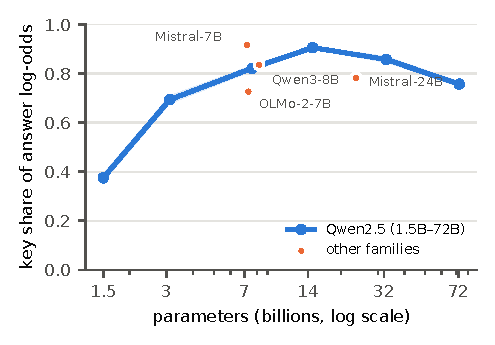
\includegraphics[width=0.55\textwidth]{figures/fig_scale.pdf}
\caption{\textbf{Key share of the \fmtOpt{} answer across scale and families.} $s_K = \bar d_K/(\bar d_K + \bar d_V)$ with keys and values clamped from layer~0. Line and band: Qwen2.5-Instruct 1.5B--72B with 95\% bootstrap CIs; points: other families. $n = 150$ stories per model; values with CIs in \cref{tab:natural}. $s_K$, the preregistered measure, includes non-specific effects; the identity key share $s_{\mathrm{ID}}$ shows the same rise to 14B and fall beyond (\cref{tab:idshare}). Exploratory (B3), with the threshold of C4.}
\label{fig:scale}
\end{figure}

\paragraph{Identity key share.} \Cref{tab:idshare} normalises $\mathrm{ID}_K$ by the total identity effect, $s_{\mathrm{ID}} = \overline{\mathrm{ID}}_K/(\overline{\mathrm{ID}}_K + \overline{\mathrm{ID}}_V)$, so that formats and models with different confidence can be compared. It tracks $s_K$ closely except under \fmtNone{} and \fmtBefore{}, where $s_K$ also counts the non-specific effect of a foreign key. Above 1.5B it is \idShareLetterMinNoOnefive{}--\idShareLetterMax{} under \fmtLetter{} and at most \idShareBeforeMax{} under \fmtBefore{} (exploratory); the table gives the other formats.

\begin{table}[!ht]
\centering
\small
\caption{\textbf{Identity key share $s_{\mathrm{ID}}$, all models} (exploratory). Ratio of mean $\mathrm{ID}_K$ to mean $\mathrm{ID}_K + \mathrm{ID}_V$, keys and values clamped from layer~0; $n = 150$ stories per format and model; 95\% bootstrap CIs, ratio recomputed in each resample.}
\label{tab:idshare}
\begin{tabular}{lccccc}
\toprule
Model & \fmtLetter & \fmtOpt & \fmtPost & \fmtNone & \fmtBefore \\
\midrule
Qwen2.5-1.5B & \begin{tabular}[t]{@{}c@{}}+0.83\\[-1pt]{\scriptsize[+0.81, +0.86]}\end{tabular} & \begin{tabular}[t]{@{}c@{}}+0.36\\[-1pt]{\scriptsize[+0.34, +0.38]}\end{tabular} & \begin{tabular}[t]{@{}c@{}}-0.08\\[-1pt]{\scriptsize[-0.10, -0.06]}\end{tabular} & \begin{tabular}[t]{@{}c@{}}+0.02\\[-1pt]{\scriptsize[+0.01, +0.02]}\end{tabular} & \begin{tabular}[t]{@{}c@{}}-0.04\\[-1pt]{\scriptsize[-0.05, -0.03]}\end{tabular} \\
Qwen2.5-3B & \begin{tabular}[t]{@{}c@{}}+0.98\\[-1pt]{\scriptsize[+0.97, +0.99]}\end{tabular} & \begin{tabular}[t]{@{}c@{}}+0.67\\[-1pt]{\scriptsize[+0.66, +0.69]}\end{tabular} & \begin{tabular}[t]{@{}c@{}}-0.00\\[-1pt]{\scriptsize[-0.04, +0.03]}\end{tabular} & \begin{tabular}[t]{@{}c@{}}+0.00\\[-1pt]{\scriptsize[-0.00, +0.01]}\end{tabular} & \begin{tabular}[t]{@{}c@{}}-0.05\\[-1pt]{\scriptsize[-0.06, -0.04]}\end{tabular} \\
Mistral-7B & \begin{tabular}[t]{@{}c@{}}+0.94\\[-1pt]{\scriptsize[+0.92, +0.95]}\end{tabular} & \begin{tabular}[t]{@{}c@{}}+0.87\\[-1pt]{\scriptsize[+0.85, +0.88]}\end{tabular} & \begin{tabular}[t]{@{}c@{}}+0.41\\[-1pt]{\scriptsize[+0.39, +0.43]}\end{tabular} & \begin{tabular}[t]{@{}c@{}}+0.04\\[-1pt]{\scriptsize[+0.03, +0.04]}\end{tabular} & \begin{tabular}[t]{@{}c@{}}+0.00\\[-1pt]{\scriptsize[-0.00, +0.00]}\end{tabular} \\
OLMo-2-7B & \begin{tabular}[t]{@{}c@{}}+0.99\\[-1pt]{\scriptsize[+0.99, +0.99]}\end{tabular} & \begin{tabular}[t]{@{}c@{}}+0.69\\[-1pt]{\scriptsize[+0.68, +0.70]}\end{tabular} & \begin{tabular}[t]{@{}c@{}}+0.19\\[-1pt]{\scriptsize[+0.17, +0.20]}\end{tabular} & \begin{tabular}[t]{@{}c@{}}+0.03\\[-1pt]{\scriptsize[+0.03, +0.04]}\end{tabular} & \begin{tabular}[t]{@{}c@{}}-0.03\\[-1pt]{\scriptsize[-0.03, -0.02]}\end{tabular} \\
Qwen2.5-7B & \begin{tabular}[t]{@{}c@{}}+0.99\\[-1pt]{\scriptsize[+0.98, +0.99]}\end{tabular} & \begin{tabular}[t]{@{}c@{}}+0.79\\[-1pt]{\scriptsize[+0.77, +0.80]}\end{tabular} & \begin{tabular}[t]{@{}c@{}}+0.32\\[-1pt]{\scriptsize[+0.30, +0.33]}\end{tabular} & \begin{tabular}[t]{@{}c@{}}+0.06\\[-1pt]{\scriptsize[+0.05, +0.06]}\end{tabular} & \begin{tabular}[t]{@{}c@{}}-0.01\\[-1pt]{\scriptsize[-0.01, -0.00]}\end{tabular} \\
Qwen3-8B & \begin{tabular}[t]{@{}c@{}}+0.97\\[-1pt]{\scriptsize[+0.97, +0.98]}\end{tabular} & \begin{tabular}[t]{@{}c@{}}+0.81\\[-1pt]{\scriptsize[+0.80, +0.82]}\end{tabular} & \begin{tabular}[t]{@{}c@{}}+0.29\\[-1pt]{\scriptsize[+0.28, +0.30]}\end{tabular} & \begin{tabular}[t]{@{}c@{}}+0.05\\[-1pt]{\scriptsize[+0.04, +0.05]}\end{tabular} & \begin{tabular}[t]{@{}c@{}}-0.01\\[-1pt]{\scriptsize[-0.02, -0.01]}\end{tabular} \\
Qwen2.5-14B & \begin{tabular}[t]{@{}c@{}}+1.00\\[-1pt]{\scriptsize[+1.00, +1.00]}\end{tabular} & \begin{tabular}[t]{@{}c@{}}+0.88\\[-1pt]{\scriptsize[+0.87, +0.89]}\end{tabular} & \begin{tabular}[t]{@{}c@{}}+0.40\\[-1pt]{\scriptsize[+0.38, +0.41]}\end{tabular} & \begin{tabular}[t]{@{}c@{}}+0.05\\[-1pt]{\scriptsize[+0.05, +0.06]}\end{tabular} & \begin{tabular}[t]{@{}c@{}}-0.00\\[-1pt]{\scriptsize[-0.01, -0.00]}\end{tabular} \\
Mistral-24B & \begin{tabular}[t]{@{}c@{}}+0.98\\[-1pt]{\scriptsize[+0.98, +0.98]}\end{tabular} & \begin{tabular}[t]{@{}c@{}}+0.73\\[-1pt]{\scriptsize[+0.72, +0.74]}\end{tabular} & \begin{tabular}[t]{@{}c@{}}+0.45\\[-1pt]{\scriptsize[+0.44, +0.46]}\end{tabular} & \begin{tabular}[t]{@{}c@{}}+0.04\\[-1pt]{\scriptsize[+0.03, +0.05]}\end{tabular} & \begin{tabular}[t]{@{}c@{}}-0.06\\[-1pt]{\scriptsize[-0.07, -0.05]}\end{tabular} \\
Qwen2.5-32B & \begin{tabular}[t]{@{}c@{}}+0.99\\[-1pt]{\scriptsize[+0.99, +0.99]}\end{tabular} & \begin{tabular}[t]{@{}c@{}}+0.82\\[-1pt]{\scriptsize[+0.81, +0.83]}\end{tabular} & \begin{tabular}[t]{@{}c@{}}+0.30\\[-1pt]{\scriptsize[+0.29, +0.32]}\end{tabular} & \begin{tabular}[t]{@{}c@{}}+0.04\\[-1pt]{\scriptsize[+0.04, +0.05]}\end{tabular} & \begin{tabular}[t]{@{}c@{}}-0.01\\[-1pt]{\scriptsize[-0.02, -0.01]}\end{tabular} \\
Qwen2.5-72B & \begin{tabular}[t]{@{}c@{}}+0.99\\[-1pt]{\scriptsize[+0.99, +0.99]}\end{tabular} & \begin{tabular}[t]{@{}c@{}}+0.71\\[-1pt]{\scriptsize[+0.70, +0.72]}\end{tabular} & \begin{tabular}[t]{@{}c@{}}+0.33\\[-1pt]{\scriptsize[+0.31, +0.34]}\end{tabular} & \begin{tabular}[t]{@{}c@{}}+0.02\\[-1pt]{\scriptsize[+0.02, +0.02]}\end{tabular} & \begin{tabular}[t]{@{}c@{}}-0.09\\[-1pt]{\scriptsize[-0.10, -0.08]}\end{tabular} \\
\bottomrule
\end{tabular}

\end{table}

\begin{figure}[!ht]
\centering
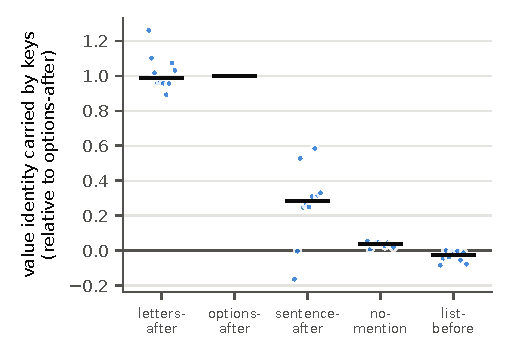
\includegraphics[width=0.55\textwidth]{figures/fig_formats.pdf}
\caption{\textbf{Key identity by format, relative to \fmtOpt{}.} Each point is one of the \nModels{} models: $\mathrm{ID}_K$ in that format divided by $\mathrm{ID}_K$ under \fmtOpt{} in the same model (so \fmtOpt{} is 1 by construction); points are jittered horizontally, and the horizontal line is the median over models. $n = 150$ stories per format and model; per-model values with 95\% bootstrap CIs are in \cref{tab:natural}.}
\label{fig:formats}
\end{figure}

\paragraph{Decomposition.} \Cref{tab:decomposition} gives, for each model and format, the effects of clamping the key, the value or both, the interaction $d_{KV} - d_K - d_V$, and $\mathrm{ID}_V$. The interaction is small relative to $d_{KV}$ in every cell, so the two channels' effects add up. Under \fmtLetter{} the value channel carries almost no identity in any model, and under \fmtNone{} and \fmtBefore{} it carries most of it: there the identity is copied. In the instruction-matched $2{\times}2$ (\cref{tab:twobytwo}), $\mathrm{ID}_K$ is larger under \fmtListA{} than under \fmtPost{} in all four models, and \fmtListA{} is close to \fmtOpt{} in the same model; neither comparison was preregistered.

\begin{table}[!ht]
\centering
\footnotesize
\caption{\textbf{Key/value decomposition.} Mean effects (nats of $m_{\mathrm{SB}}$) of clamping the writing token's key ($d_K$), value ($d_V$) or both ($d_{KV}$) to the source run's from layer~0, measured against the self-clamp row; the interaction $d_{KV} - d_K - d_V$ with its 95\% bootstrap CI; and the value identity $\mathrm{ID}_V$ (nats). $n = 150$ stories per format and model.}
\label{tab:decomposition}
\begin{tabular}{llrrrrr}
\toprule
Model & Format & $d_K$ & $d_V$ & $d_{KV}$ & interaction & $\mathrm{ID}_V$ \\
\midrule
Qwen2.5-1.5B & letters- after & +9.9 & +4.2 & +14.5 & +0.4 \tiny[-0.5, +1.3] & +0.7 \\
 & options- after & +6.3 & +10.4 & +16.7 & -0.0 \tiny[-0.5, +0.5] & +5.0 \\
 & sentence- after & +0.5 & +14.4 & +14.8 & -0.0 \tiny[-0.4, +0.3] & +6.5 \\
 & no- mention & +1.8 & +21.8 & +23.5 & -0.1 \tiny[-0.7, +0.5] & +10.2 \\
 & list- before & +1.2 & +13.6 & +14.5 & -0.3 \tiny[-0.6, +0.1] & +5.9 \\
\midrule
Qwen2.5-3B & letters- after & +22.3 & +0.8 & +22.8 & -0.4 \tiny[-1.1, +0.3] & +0.2 \\
 & options- after & +20.4 & +9.0 & +29.1 & -0.4 \tiny[-1.1, +0.3] & +5.0 \\
 & sentence- after & +2.9 & +26.8 & +29.9 & +0.2 \tiny[-0.6, +1.0] & +11.8 \\
 & no- mention & +4.3 & +41.1 & +45.9 & +0.5 \tiny[-0.1, +1.1] & +18.1 \\
 & list- before & +2.8 & +23.4 & +26.4 & +0.2 \tiny[-0.5, +0.8] & +9.6 \\
\midrule
Mistral-7B & letters- after & +31.3 & +1.5 & +32.2 & -0.5 \tiny[-1.2, +0.1] & +1.0 \\
 & options- after & +28.0 & +2.6 & +30.8 & +0.1 \tiny[-0.6, +0.8] & +2.3 \\
 & sentence- after & +12.9 & +19.5 & +31.8 & -0.6 \tiny[-2.3, +1.1] & +11.5 \\
 & no- mention & +2.7 & +28.8 & +31.5 & -0.1 \tiny[-0.4, +0.3] & +13.6 \\
 & list- before & +1.2 & +30.9 & +32.1 & +0.1 \tiny[-0.3, +0.5] & +14.6 \\
\midrule
OLMo-2-7B & letters- after & +15.6 & +0.1 & +15.7 & +0.0 \tiny[-0.1, +0.1] & +0.1 \\
 & options- after & +15.5 & +5.8 & +21.0 & -0.3 \tiny[-0.9, +0.2] & +3.7 \\
 & sentence- after & +3.8 & +16.8 & +20.7 & +0.0 \tiny[-0.5, +0.6] & +8.6 \\
 & no- mention & +2.7 & +23.5 & +26.1 & -0.1 \tiny[-0.5, +0.3] & +11.0 \\
 & list- before & +0.2 & +23.6 & +23.9 & +0.1 \tiny[-0.1, +0.4] & +11.2 \\
\midrule
Qwen2.5-7B & letters- after & +40.2 & +1.1 & +41.2 & -0.1 \tiny[-0.7, +0.4] & +0.2 \\
 & options- after & +39.6 & +8.6 & +47.9 & -0.4 \tiny[-1.1, +0.3] & +5.8 \\
 & sentence- after & +11.0 & +23.1 & +34.4 & +0.4 \tiny[-0.4, +1.1] & +11.9 \\
 & no- mention & +6.0 & +36.8 & +42.5 & -0.3 \tiny[-0.7, +0.2] & +16.6 \\
 & list- before & +2.4 & +34.8 & +36.8 & -0.4 \tiny[-0.8, -0.1] & +16.0 \\
\midrule
Qwen3-8B & letters- after & +66.8 & +1.2 & +67.9 & -0.1 \tiny[-0.5, +0.3] & +1.0 \\
 & options- after & +67.1 & +13.2 & +80.5 & +0.2 \tiny[-1.4, +1.7] & +8.2 \\
 & sentence- after & +14.3 & +40.0 & +53.3 & -1.1 \tiny[-2.5, +0.3] & +21.8 \\
 & no- mention & +5.7 & +54.4 & +59.4 & -0.7 \tiny[-1.6, +0.2] & +25.3 \\
 & list- before & +2.9 & +51.8 & +54.4 & -0.3 \tiny[-0.8, +0.2] & +24.0 \\
\midrule
Qwen2.5-14B & letters- after & +70.0 & +0.2 & +70.2 & +0.0 \tiny[-0.2, +0.3] & +0.1 \\
 & options- after & +75.0 & +7.8 & +82.8 & -0.1 \tiny[-0.7, +0.5] & +5.4 \\
 & sentence- after & +21.9 & +33.8 & +56.9 & +1.1 \tiny[-1.4, +3.6] & +18.5 \\
 & no- mention & +10.8 & +46.5 & +57.1 & -0.2 \tiny[-0.9, +0.4] & +19.1 \\
 & list- before & +2.4 & +65.9 & +68.3 & +0.0 \tiny[-0.5, +0.5] & +31.1 \\
\midrule
Mistral-24B & letters- after & +18.7 & +0.4 & +19.0 & -0.1 \tiny[-0.2, -0.0] & +0.2 \\
 & options- after & +17.1 & +4.8 & +21.9 & +0.1 \tiny[-0.2, +0.4] & +3.6 \\
 & sentence- after & +8.1 & +10.4 & +18.6 & +0.1 \tiny[-0.7, +0.8] & +6.8 \\
 & no- mention & +2.0 & +20.8 & +22.6 & -0.2 \tiny[-0.4, +0.0] & +9.8 \\
 & list- before & -0.0 & +19.4 & +19.4 & +0.1 \tiny[-0.1, +0.3] & +9.1 \\
\midrule
Qwen2.5-32B & letters- after & +69.5 & +0.6 & +70.3 & +0.2 \tiny[-0.1, +0.5] & +0.3 \\
 & options- after & +61.4 & +10.2 & +71.6 & -0.1 \tiny[-1.8, +1.7] & +7.1 \\
 & sentence- after & +18.7 & +44.8 & +63.1 & -0.4 \tiny[-2.0, +1.3] & +23.4 \\
 & no- mention & +9.8 & +53.8 & +63.4 & -0.2 \tiny[-0.9, +0.5] & +23.4 \\
 & list- before & +2.8 & +65.1 & +68.1 & +0.1 \tiny[-0.5, +0.7] & +30.6 \\
\midrule
Qwen2.5-72B & letters- after & +52.8 & +0.2 & +53.0 & -0.0 \tiny[-0.2, +0.2] & +0.3 \\
 & options- after & +44.6 & +14.3 & +59.6 & +0.7 \tiny[-0.3, +1.7] & +10.5 \\
 & sentence- after & +14.4 & +30.9 & +46.4 & +1.1 \tiny[-0.3, +2.6] & +17.5 \\
 & no- mention & +3.1 & +47.7 & +50.9 & +0.1 \tiny[-0.4, +0.5] & +22.9 \\
 & list- before & -1.7 & +51.2 & +49.8 & +0.3 \tiny[-0.2, +0.7] & +24.1 \\
\bottomrule
\end{tabular}

\end{table}

\paragraph{Clamp onset.} Layer-0 keys are a function of the input embedding alone, so \cref{tab:onset} starts both clamps deeper (exploratory). With $\ell_0 \approx 0.06L$ the shares are essentially unchanged in eight of ten models. With $\ell_0 \approx 0.3L$ the share stays at or above one half in seven models (up to \onsetLateQwenFourteen{} at Qwen2.5-14B), but falls to \onsetLateQwenOnefive{} at Qwen2.5-1.5B, \onsetLateMistralTwentyfour{} at Mistral-Small-24B and \onsetLateOlmoSeven{} at OLMo-2-7B, where the key effect depends on the lowest layers. Deeper keys therefore still carry the written word in most models. With $\ell_0 > 0$ the clamp is no longer exact, and at $\ell_0 \approx 0.3L$ the key and value effects no longer add up: the interaction is positive in every model (result summaries). The share at that onset is therefore descriptive only.

\begin{table}[!ht]
\centering
\caption{\textbf{Key share by clamp onset.} $s_K = \bar d_K / (\bar d_K + \bar d_V)$ under \fmtOpt{} with both clamps applied from layer $\ell_0$ on; the onset used in each model is given in brackets. $n = 150$ stories per model; point estimates (the $\ell_0 = 0$ intervals are in \cref{tab:natural}). Exploratory.}
\label{tab:onset}
\begin{tabular}{lcccc}
\toprule
Model & layers $L$ & $s_K$, onset $\ell_0{=}0$ & $s_K$, $\ell_0{\approx}0.06L$ & $s_K$, $\ell_0{\approx}0.3L$ \\
\midrule
Qwen2.5-1.5B & 28 & 0.37 ($\ell_0{=}0$) & 0.37 ($\ell_0{=}2$) & 0.19 ($\ell_0{=}8$) \\
Qwen2.5-3B & 36 & 0.69 ($\ell_0{=}0$) & 0.69 ($\ell_0{=}2$) & 0.56 ($\ell_0{=}11$) \\
Mistral-7B & 32 & 0.92 ($\ell_0{=}0$) & 0.91 ($\ell_0{=}2$) & 0.53 ($\ell_0{=}10$) \\
OLMo-2-7B & 32 & 0.73 ($\ell_0{=}0$) & 0.72 ($\ell_0{=}2$) & 0.03 ($\ell_0{=}10$) \\
Qwen2.5-7B & 28 & 0.82 ($\ell_0{=}0$) & 0.82 ($\ell_0{=}2$) & 0.66 ($\ell_0{=}8$) \\
Qwen3-8B & 36 & 0.84 ($\ell_0{=}0$) & 0.84 ($\ell_0{=}2$) & 0.73 ($\ell_0{=}11$) \\
Qwen2.5-14B & 48 & 0.91 ($\ell_0{=}0$) & 0.91 ($\ell_0{=}3$) & 0.83 ($\ell_0{=}14$) \\
Mistral-24B & 40 & 0.78 ($\ell_0{=}0$) & 0.78 ($\ell_0{=}2$) & 0.37 ($\ell_0{=}12$) \\
Qwen2.5-32B & 64 & 0.86 ($\ell_0{=}0$) & 0.86 ($\ell_0{=}4$) & 0.82 ($\ell_0{=}19$) \\
Qwen2.5-72B & 80 & 0.76 ($\ell_0{=}0$) & 0.76 ($\ell_0{=}5$) & 0.55 ($\ell_0{=}24$) \\
\bottomrule
\end{tabular}

\end{table}

\paragraph{Layer windows and KV groups.} \Cref{tab:windows} refines the row-restricted splice at Qwen2.5-1.5B (28 layers, two KV groups). Only the option-word rows see the source key, and the swap is further limited to a window of four layers (all KV groups) or to one KV group's slice of the key (all layers). The read happens in layers 4--15, and KV group 1 carries more of it than KV group 0 in both formats. The seven windows together recover less than the option-word rows do with the swap at all layers, and the two single-group swaps together recover less than both groups at once, so the read compounds across layers and groups. We ran the same window and KV-group splices, on the option-word rows under \fmtOpt{} and \fmtLetter{}, at Qwen2.5-7B, Qwen2.5-14B and Mistral-7B (exploratory; result summaries). In these models no single four-layer window and no single KV group recovers most of the option-word effect, so the dominance of one KV group seen at 1.5B does not carry over.

\begin{table}[!ht]
\centering
\caption{\textbf{Depth and KV-group localisation of the option-word key read} (Qwen2.5-1.5B, FP32). Entries are fractions of the effect obtained when the option-word rows see the source key in every layer and both KV groups, with 95\% bootstrap CIs over stories (ratio of means recomputed in each resample). $n = 40$ stories per format. Exploratory.}
\label{tab:windows}
\begin{tabular}{lcc}
\toprule
Rows/layers that see the swapped key & \fmtOpt & \fmtLetter \\
\midrule
layers 0--3 & $-$0.02 \tiny[$-$0.02, $-$0.01] & $-$0.01 \tiny[$-$0.01, 0.00] \\
layers 4--7 & +0.23 \tiny[+0.11, +0.35] & +0.36 \tiny[+0.26, +0.46] \\
layers 8--11 & +0.14 \tiny[+0.10, +0.18] & +0.06 \tiny[+0.03, +0.09] \\
layers 12--15 & +0.15 \tiny[+0.12, +0.19] & +0.04 \tiny[+0.02, +0.06] \\
layers 16--19 & +0.02 \tiny[+0.01, +0.04] & +0.01 \tiny[0.00, +0.02] \\
layers 20--23 & 0.00 \tiny[0.00, 0.00] & 0.00 \tiny[0.00, 0.00] \\
layers 24--27 & 0.00 \tiny[0.00, 0.00] & 0.00 \tiny[0.00, 0.00] \\
KV group 0 (all layers) & +0.22 \tiny[+0.17, +0.27] & +0.06 \tiny[+0.03, +0.09] \\
KV group 1 (all layers) & +0.53 \tiny[+0.40, +0.66] & +0.66 \tiny[+0.57, +0.75] \\
\bottomrule
\end{tabular}

\end{table}

\paragraph{New tasks.} \Cref{tab:tasks} gives the paint and schedule results. In every model and both tasks, $\mathrm{ID}_K$ is large under \fmtLetter{} and \fmtOpt{}, intermediate under \fmtPost{}, small under \fmtNone{} and near zero under \fmtBefore{}. The \fmtOpt{} key share ranges from \taskPaintShareMin{} to \taskPaintShareMax{} (paint) and from \taskScheduleShareMin{} to \taskScheduleShareMax{} (schedule), lowest at OLMo-2-7B in both.

\begin{table}[!ht]
\centering
\caption{\textbf{Paint and schedule tasks.} Key share under \fmtOpt{} and $\mathrm{ID}_K$ (nats) in each format, clamped from layer~0. $n = 150$ stories per task, format and model; 95\% bootstrap CIs. Preregistration D (D1, D2) for \fmtOpt{}, \fmtNone{} and \fmtBefore{}; the rest exploratory.}
\label{tab:tasks}
\resizebox{\textwidth}{!}{\begin{tabular}{llcccccc}
\toprule
Task & Model & $s_K$ (\fmtOpt) & \multicolumn{5}{c}{$\mathrm{ID}_K$ (nats)} \\
\cmidrule(lr){4-8}
 & & & \fmtLetter & \fmtOpt & \fmtPost & \fmtNone & \fmtBefore \\
\midrule
paint & Qwen2.5-7B & \begin{tabular}[t]{@{}c@{}}0.73\\[-1pt]{\scriptsize[0.72, 0.74]}\end{tabular} & \begin{tabular}[t]{@{}c@{}}+21.5\\[-1pt]{\scriptsize[+21.3, +21.7]}\end{tabular} & \begin{tabular}[t]{@{}c@{}}+21.4\\[-1pt]{\scriptsize[+21.2, +21.7]}\end{tabular} & \begin{tabular}[t]{@{}c@{}}+3.0\\[-1pt]{\scriptsize[+2.8, +3.1]}\end{tabular} & \begin{tabular}[t]{@{}c@{}}+1.2\\[-1pt]{\scriptsize[+1.1, +1.3]}\end{tabular} & \begin{tabular}[t]{@{}c@{}}+0.3\\[-1pt]{\scriptsize[+0.2, +0.4]}\end{tabular} \\
 & Qwen2.5-14B & \begin{tabular}[t]{@{}c@{}}0.90\\[-1pt]{\scriptsize[0.90, 0.91]}\end{tabular} & \begin{tabular}[t]{@{}c@{}}+35.7\\[-1pt]{\scriptsize[+35.4, +36.0]}\end{tabular} & \begin{tabular}[t]{@{}c@{}}+40.3\\[-1pt]{\scriptsize[+39.9, +40.8]}\end{tabular} & \begin{tabular}[t]{@{}c@{}}+3.5\\[-1pt]{\scriptsize[+3.3, +3.7]}\end{tabular} & \begin{tabular}[t]{@{}c@{}}+0.8\\[-1pt]{\scriptsize[+0.7, +0.9]}\end{tabular} & \begin{tabular}[t]{@{}c@{}}+0.2\\[-1pt]{\scriptsize[+0.1, +0.2]}\end{tabular} \\
 & Qwen3-8B & \begin{tabular}[t]{@{}c@{}}0.92\\[-1pt]{\scriptsize[0.92, 0.93]}\end{tabular} & \begin{tabular}[t]{@{}c@{}}+39.7\\[-1pt]{\scriptsize[+39.4, +40.1]}\end{tabular} & \begin{tabular}[t]{@{}c@{}}+42.7\\[-1pt]{\scriptsize[+42.3, +43.0]}\end{tabular} & \begin{tabular}[t]{@{}c@{}}+4.9\\[-1pt]{\scriptsize[+4.7, +5.2]}\end{tabular} & \begin{tabular}[t]{@{}c@{}}+1.1\\[-1pt]{\scriptsize[+1.0, +1.2]}\end{tabular} & \begin{tabular}[t]{@{}c@{}}+0.1\\[-1pt]{\scriptsize[+0.1, +0.2]}\end{tabular} \\
 & Mistral-7B & \begin{tabular}[t]{@{}c@{}}0.86\\[-1pt]{\scriptsize[0.85, 0.87]}\end{tabular} & \begin{tabular}[t]{@{}c@{}}+16.0\\[-1pt]{\scriptsize[+15.7, +16.3]}\end{tabular} & \begin{tabular}[t]{@{}c@{}}+16.1\\[-1pt]{\scriptsize[+15.9, +16.4]}\end{tabular} & \begin{tabular}[t]{@{}c@{}}+2.2\\[-1pt]{\scriptsize[+1.9, +2.4]}\end{tabular} & \begin{tabular}[t]{@{}c@{}}+0.4\\[-1pt]{\scriptsize[+0.3, +0.5]}\end{tabular} & \begin{tabular}[t]{@{}c@{}}+0.1\\[-1pt]{\scriptsize[+0.1, +0.2]}\end{tabular} \\
 & OLMo-2-7B & \begin{tabular}[t]{@{}c@{}}0.47\\[-1pt]{\scriptsize[0.46, 0.48]}\end{tabular} & \begin{tabular}[t]{@{}c@{}}+7.4\\[-1pt]{\scriptsize[+7.2, +7.5]}\end{tabular} & \begin{tabular}[t]{@{}c@{}}+6.5\\[-1pt]{\scriptsize[+6.3, +6.7]}\end{tabular} & \begin{tabular}[t]{@{}c@{}}+0.7\\[-1pt]{\scriptsize[+0.6, +0.8]}\end{tabular} & \begin{tabular}[t]{@{}c@{}}+0.1\\[-1pt]{\scriptsize[+0.1, +0.2]}\end{tabular} & \begin{tabular}[t]{@{}c@{}}-0.1\\[-1pt]{\scriptsize[-0.1, -0.1]}\end{tabular} \\
\midrule
schedule & Qwen2.5-7B & \begin{tabular}[t]{@{}c@{}}0.58\\[-1pt]{\scriptsize[0.56, 0.59]}\end{tabular} & \begin{tabular}[t]{@{}c@{}}+19.6\\[-1pt]{\scriptsize[+19.3, +20.0]}\end{tabular} & \begin{tabular}[t]{@{}c@{}}+12.7\\[-1pt]{\scriptsize[+12.4, +13.0]}\end{tabular} & \begin{tabular}[t]{@{}c@{}}+4.1\\[-1pt]{\scriptsize[+3.8, +4.4]}\end{tabular} & \begin{tabular}[t]{@{}c@{}}+0.1\\[-1pt]{\scriptsize[+0.1, +0.2]}\end{tabular} & \begin{tabular}[t]{@{}c@{}}-0.1\\[-1pt]{\scriptsize[-0.2, -0.1]}\end{tabular} \\
 & Qwen2.5-14B & \begin{tabular}[t]{@{}c@{}}0.87\\[-1pt]{\scriptsize[0.87, 0.88]}\end{tabular} & \begin{tabular}[t]{@{}c@{}}+35.6\\[-1pt]{\scriptsize[+35.3, +35.9]}\end{tabular} & \begin{tabular}[t]{@{}c@{}}+26.1\\[-1pt]{\scriptsize[+25.7, +26.5]}\end{tabular} & \begin{tabular}[t]{@{}c@{}}+10.9\\[-1pt]{\scriptsize[+10.3, +11.6]}\end{tabular} & \begin{tabular}[t]{@{}c@{}}+0.6\\[-1pt]{\scriptsize[+0.5, +0.6]}\end{tabular} & \begin{tabular}[t]{@{}c@{}}+0.2\\[-1pt]{\scriptsize[+0.1, +0.2]}\end{tabular} \\
 & Qwen3-8B & \begin{tabular}[t]{@{}c@{}}0.92\\[-1pt]{\scriptsize[0.91, 0.92]}\end{tabular} & \begin{tabular}[t]{@{}c@{}}+39.6\\[-1pt]{\scriptsize[+39.2, +40.0]}\end{tabular} & \begin{tabular}[t]{@{}c@{}}+28.5\\[-1pt]{\scriptsize[+28.0, +29.0]}\end{tabular} & \begin{tabular}[t]{@{}c@{}}+7.3\\[-1pt]{\scriptsize[+6.9, +7.7]}\end{tabular} & \begin{tabular}[t]{@{}c@{}}+0.9\\[-1pt]{\scriptsize[+0.8, +1.0]}\end{tabular} & \begin{tabular}[t]{@{}c@{}}+0.2\\[-1pt]{\scriptsize[+0.1, +0.2]}\end{tabular} \\
 & Mistral-7B & \begin{tabular}[t]{@{}c@{}}0.82\\[-1pt]{\scriptsize[0.81, 0.84]}\end{tabular} & \begin{tabular}[t]{@{}c@{}}+16.2\\[-1pt]{\scriptsize[+15.6, +16.7]}\end{tabular} & \begin{tabular}[t]{@{}c@{}}+13.2\\[-1pt]{\scriptsize[+12.9, +13.5]}\end{tabular} & \begin{tabular}[t]{@{}c@{}}+5.1\\[-1pt]{\scriptsize[+4.6, +5.6]}\end{tabular} & \begin{tabular}[t]{@{}c@{}}+0.1\\[-1pt]{\scriptsize[+0.1, +0.2]}\end{tabular} & \begin{tabular}[t]{@{}c@{}}-0.0\\[-1pt]{\scriptsize[-0.1, +0.0]}\end{tabular} \\
 & OLMo-2-7B & \begin{tabular}[t]{@{}c@{}}0.35\\[-1pt]{\scriptsize[0.34, 0.37]}\end{tabular} & \begin{tabular}[t]{@{}c@{}}+7.4\\[-1pt]{\scriptsize[+7.2, +7.6]}\end{tabular} & \begin{tabular}[t]{@{}c@{}}+4.5\\[-1pt]{\scriptsize[+4.3, +4.7]}\end{tabular} & \begin{tabular}[t]{@{}c@{}}+2.3\\[-1pt]{\scriptsize[+2.1, +2.4]}\end{tabular} & \begin{tabular}[t]{@{}c@{}}+0.1\\[-1pt]{\scriptsize[+0.1, +0.1]}\end{tabular} & \begin{tabular}[t]{@{}c@{}}+0.0\\[-1pt]{\scriptsize[-0.0, +0.1]}\end{tabular} \\
\bottomrule
\end{tabular}
}
\end{table}

\paragraph{Role control.} Could the writing token's channels carry more than identity, such as whether the person asked about saw the move? The role-swap control exchanges the observer's and the non-observer's names but keeps the location word (\cref{app:prompts}). \Cref{tab:role} gives the role-swap effect and the fractions of it that the writing token's key and value carry. The swap shifts the belief answer by \roleEffMin{} to \roleEffMax{} nats, depending on model and format, and clamping either channel alone to the role-swapped run carries at most \roleFracMax{} of that shift, under \fmtOpt{}, \fmtNone{} and \fmtLetter{}, in five models including Qwen2.5-72B. The prediction was preregistered for \fmtOpt{} and \fmtNone{} in four models, with a bound of 0.15 (E2, met); \fmtLetter{} and Qwen2.5-72B are exploratory. The writing token's key and value thus carry \emph{which} value was written, not the observer's name; an ordering-ID address of the observer, the same in both runs, would not register (\cref{app:discussion}).

\begin{table}[!ht]
\centering
\caption{\textbf{Identity, not belief role.} Role effect: mean change in $m = \log p(\text{initial}) - \log p(\textsc{loc})$ when the observer and non-observer are swapped with the same location word (nats). $f_K$, $f_V$: fraction of that change reproduced by clamping only the writing token's key or value (all layers) to the role-swapped run's, as a ratio of means. Direct question; $n = 150$ stories per format and model; 95\% bootstrap CIs. Preregistration E (E2) for \fmtOpt{} and \fmtNone{} in the four 7--14B models; \fmtLetter{} and Qwen2.5-72B exploratory.}
\label{tab:role}
\begin{tabular}{llccc}
\toprule
Model & Format & role effect (nats) & $f_K$ & $f_V$ \\
\midrule
Qwen2.5-7B & options- after & +34.4 & +0.006 & +0.010 \\
 & no- mention & +28.7 & +0.014 & +0.001 \\
 & letters- after & +29.8 & +0.003 & +0.018 \\
\midrule
Qwen2.5-14B & options- after & +79.8 & +0.001 & -0.000 \\
 & no- mention & +51.4 & +0.001 & -0.000 \\
 & letters- after & +66.0 & -0.000 & -0.000 \\
\midrule
Mistral-7B & options- after & +28.4 & +0.003 & +0.004 \\
 & no- mention & +26.6 & +0.019 & +0.001 \\
 & letters- after & +28.9 & +0.000 & +0.011 \\
\midrule
OLMo-2-7B & options- after & +16.9 & +0.004 & +0.002 \\
 & no- mention & +17.7 & +0.014 & +0.002 \\
 & letters- after & +12.5 & -0.000 & +0.003 \\
\midrule
Qwen2.5-72B & options- after & +50.6 & +0.001 & +0.002 \\
 & no- mention & +38.4 & +0.007 & -0.001 \\
 & letters- after & +46.8 & -0.001 & +0.003 \\
\bottomrule
\end{tabular}

\end{table}

\paragraph{Competent-only analysis.} Our primary analyses pool all stories, whether or not the model answers the clean runs correctly. As a secondary analysis, every natural-factorial quantity is also computed on the stories whose base and source clean runs are both answered correctly (argmax over the candidates). From 7B up most stories are competent and the two analyses agree closely. The competent subset is smallest at Qwen2.5-1.5B and 3B, and the estimates move most at 3B. The sign of $\mathrm{ID}_K$ under \fmtOpt{}, \fmtLetter{}, \fmtNone{} and \fmtBefore{} is unchanged in every model. The near-zero \fmtPost{} value at Qwen2.5-3B becomes slightly positive, with a CI that excludes zero, but stays far below the \fmtPost{} values from 7B up. No conclusion in the main text changes.

\subsection{Fresh stories}\label{app:fresh}

\paragraph{Design.} The fresh stories (\cref{app:prompts-fresh}) were run in eight models: the four discovery-sample models of the instruction-matched $2{\times}2$ (Qwen2.5-7B, Qwen2.5-14B, Mistral-7B, OLMo-2-7B; lines with the suffix P4f, which must hold in every evaluable model, at 95\,\%) and four model families never examined before (Llama-3.1-8B, Gemma-2-9B, Phi-4, Falcon3-7B; lines with the suffix N4, which need three of the four, at 98.75\,\%), plus Gemma-2-2B for the sentence read at small scale. Every statistic uses the emitted-form score (\cref{app:emitted}); its coverage was at least \JbGfourCovMin{} in every cell, so no statistic fell back to its behavioural counterpart. Intervals are two-stage bootstrap intervals over the 55 (lexicon, base, source) cells and the cores within them. They have two limits. For rates at or near 0 or 1 (many $\beta$ cells, and OLMo-2-7B's three flips in 150 stories, where 11.9\,\% of the resamples are exactly zero) percentile intervals are degenerate or unreliable; and with about 2.7 stories per cell, resampling the stories within each drawn cell adds variance, which is conservative for the lines that held but makes near-threshold failures (OLMo-2-7B's sentence read in generated answers) look less certain than they are. Cluster-adjusted exact intervals for these rates were not computed. Generated accuracy on the clean base run was at least \JbGfiveAccMin{} in every arm of the eight models. \Cref{tab:fresh} gives every model and arm. % verbatim: 55 cells, entry J part B

\begin{table}[!ht]
\centering
\footnotesize
\caption{\textbf{Fresh stories, eight models.} 150 fresh cores per model; emitted-form score; 95\,\% two-stage cluster-bootstrap intervals (the N4 lines are decided on 98.75\,\% bounds, given in the text). Arms: AFTER = \fmtListA{}, POST = \fmtPost{}, POST-NULL = \fmtNull{}, PRE = \fmtSentB{}, BEFORE = \fmtBefore{}, NONE = \fmtNone{}. $r$: $\overline{\mathrm{ID}}_K$ in the arm divided by $\overline{\mathrm{ID}}_K$ under AFTER (1 by definition there); $s_{\mathrm{ID}}$: the key share of the value's identity; $\beta_K$, $\beta_V$: the share of generated answers that move to the clamped value under the key-only or value-only clamp, net of moves to it under the clamp to the other of S and X. The first four models are the discovery-sample models (P4), the next four the new families (N4).}
\label{tab:fresh}
{\scriptsize\setlength{\tabcolsep}{5pt}\begin{tabular}{llcccc}
\toprule
Model & Arm & $r$ & $s_{\mathrm{ID}}$ & $\beta_K$ & $\beta_V$ \\
\midrule
Qwen2.5-7B & AFTER & 1 & 0.79 [0.77, 0.81] & 0.99 [0.98, 1.00] & 0.00 [0.00, 0.00] \\
Qwen2.5-7B & POST & 0.27 [0.24, 0.30] & 0.33 [0.30, 0.35] & 0.11 [0.06, 0.16] & 0.86 [0.79, 0.92] \\
Qwen2.5-7B & POST-NULL & 0.03 [0.02, 0.04] & 0.04 [0.03, 0.05] & 0.00 [0.00, 0.00] & 0.92 [0.86, 0.96] \\
Qwen2.5-7B & PRE & -0.01 [-0.02, -0.01] & -0.02 [-0.03, -0.01] & 0.00 [0.00, 0.00] & 1.00 [1.00, 1.00] \\
Qwen2.5-7B & BEFORE & -0.02 [-0.02, -0.01] & -0.02 [-0.03, -0.01] & 0.00 [0.00, 0.00] & 0.96 [0.93, 0.99] \\
Qwen2.5-7B & NONE & 0.03 [0.02, 0.04] & 0.04 [0.03, 0.04] & 0.00 [0.00, 0.00] & 0.97 [0.95, 0.99] \\
\midrule
Qwen2.5-14B & AFTER & 1 & 0.88 [0.86, 0.89] & 1.00 [1.00, 1.00] & 0.00 [0.00, 0.00] \\
Qwen2.5-14B & POST & 0.39 [0.36, 0.43] & 0.39 [0.36, 0.41] & 0.23 [0.16, 0.31] & 0.75 [0.66, 0.83] \\
Qwen2.5-14B & POST-NULL & 0.03 [0.02, 0.04] & 0.05 [0.04, 0.06] & 0.00 [0.00, 0.00] & 0.99 [0.97, 1.00] \\
Qwen2.5-14B & PRE & -0.00 [-0.01, 0.00] & -0.00 [-0.01, 0.00] & 0.00 [0.00, 0.00] & 1.00 [1.00, 1.00] \\
Qwen2.5-14B & BEFORE & -0.00 [-0.01, 0.00] & -0.00 [-0.01, 0.00] & 0.00 [0.00, 0.00] & 1.00 [1.00, 1.00] \\
Qwen2.5-14B & NONE & 0.03 [0.02, 0.04] & 0.05 [0.04, 0.06] & 0.00 [0.00, 0.00] & 0.99 [0.97, 1.00] \\
\midrule
Mistral-7B & AFTER & 1 & 0.80 [0.78, 0.82] & 0.95 [0.91, 0.98] & 0.05 [0.02, 0.09] \\
Mistral-7B & POST & 0.57 [0.50, 0.63] & 0.40 [0.37, 0.43] & 0.31 [0.23, 0.40] & 0.71 [0.62, 0.79] \\
Mistral-7B & POST-NULL & -0.00 [-0.01, 0.01] & -0.00 [-0.01, 0.01] & 0.00 [0.00, 0.00] & 0.93 [0.88, 0.97] \\
Mistral-7B & PRE & -0.03 [-0.05, -0.02] & -0.03 [-0.05, -0.02] & 0.00 [0.00, 0.00] & 0.99 [0.97, 1.00] \\
Mistral-7B & BEFORE & -0.02 [-0.03, -0.01] & -0.02 [-0.03, -0.01] & 0.00 [0.00, 0.00] & 0.98 [0.96, 1.00] \\
Mistral-7B & NONE & -0.00 [-0.01, 0.01] & -0.00 [-0.01, 0.01] & 0.00 [0.00, 0.00] & 0.97 [0.94, 0.99] \\
\midrule
OLMo-2-7B & AFTER & 1 & 0.63 [0.61, 0.65] & 0.86 [0.80, 0.92] & 0.13 [0.07, 0.19] \\
OLMo-2-7B & POST & 0.18 [0.14, 0.22] & 0.16 [0.13, 0.19] & 0.01 [0.00, 0.03] & 0.96 [0.93, 0.99] \\
OLMo-2-7B & POST-NULL & 0.07 [0.05, 0.09] & 0.06 [0.05, 0.07] & 0.00 [0.00, 0.00] & 0.74 [0.66, 0.82] \\
OLMo-2-7B & PRE & -0.05 [-0.07, -0.04] & -0.05 [-0.06, -0.04] & 0.00 [0.00, 0.00] & 1.00 [0.99, 1.00] \\
OLMo-2-7B & BEFORE & -0.04 [-0.06, -0.03] & -0.04 [-0.05, -0.03] & 0.00 [0.00, 0.00] & 1.00 [0.99, 1.00] \\
OLMo-2-7B & NONE & 0.07 [0.05, 0.08] & 0.05 [0.04, 0.06] & 0.00 [0.00, 0.00] & 0.81 [0.74, 0.88] \\
\midrule
Llama-3.1-8B & AFTER & 1 & 0.61 [0.59, 0.63] & 0.76 [0.69, 0.83] & 0.14 [0.08, 0.22] \\
Llama-3.1-8B & POST & 0.40 [0.35, 0.44] & 0.29 [0.26, 0.32] & 0.09 [0.04, 0.13] & 0.88 [0.82, 0.94] \\
Llama-3.1-8B & POST-NULL & 0.12 [0.09, 0.15] & 0.08 [0.06, 0.09] & 0.00 [0.00, 0.00] & 0.90 [0.84, 0.95] \\
Llama-3.1-8B & PRE & -0.03 [-0.05, -0.01] & -0.02 [-0.04, -0.01] & 0.00 [0.00, 0.00] & 1.00 [1.00, 1.00] \\
Llama-3.1-8B & BEFORE & -0.06 [-0.08, -0.05] & -0.05 [-0.07, -0.04] & 0.00 [0.00, 0.00] & 1.00 [1.00, 1.00] \\
Llama-3.1-8B & NONE & 0.11 [0.08, 0.14] & 0.07 [0.06, 0.09] & 0.00 [0.00, 0.00] & 0.88 [0.81, 0.93] \\
\midrule
Gemma-2-9B & AFTER & 1 & 0.70 [0.69, 0.71] & 1.00 [0.99, 1.00] & 0.00 [0.00, 0.00] \\
Gemma-2-9B & POST & 0.51 [0.47, 0.55] & 0.36 [0.34, 0.38] & 0.13 [0.09, 0.19] & 0.84 [0.77, 0.89] \\
Gemma-2-9B & POST-NULL & 0.00 [-0.00, 0.01] & 0.00 [-0.00, 0.01] & 0.00 [0.00, 0.00] & 1.00 [1.00, 1.00] \\
Gemma-2-9B & PRE & -0.02 [-0.03, -0.01] & -0.02 [-0.03, -0.02] & 0.00 [0.00, 0.00] & 1.00 [1.00, 1.00] \\
Gemma-2-9B & BEFORE & -0.02 [-0.02, -0.01] & -0.02 [-0.03, -0.02] & 0.00 [0.00, 0.00] & 1.00 [1.00, 1.00] \\
Gemma-2-9B & NONE & 0.01 [-0.00, 0.01] & 0.00 [-0.00, 0.01] & 0.00 [0.00, 0.00] & 1.00 [1.00, 1.00] \\
\midrule
Phi-4 & AFTER & 1 & 0.72 [0.71, 0.74] & 0.99 [0.97, 1.00] & 0.02 [0.00, 0.04] \\
Phi-4 & POST & 0.33 [0.30, 0.37] & 0.28 [0.26, 0.30] & 0.03 [0.01, 0.06] & 0.97 [0.94, 0.99] \\
Phi-4 & POST-NULL & 0.00 [-0.01, 0.01] & 0.00 [-0.01, 0.01] & 0.00 [0.00, 0.00] & 0.97 [0.92, 1.00] \\
Phi-4 & PRE & -0.03 [-0.03, -0.02] & -0.03 [-0.03, -0.02] & 0.00 [0.00, 0.00] & 1.00 [1.00, 1.00] \\
Phi-4 & BEFORE & -0.05 [-0.05, -0.04] & -0.06 [-0.08, -0.05] & 0.00 [0.00, 0.00] & 0.96 [0.92, 0.99] \\
Phi-4 & NONE & 0.01 [-0.00, 0.02] & 0.01 [-0.00, 0.01] & 0.00 [0.00, 0.00] & 0.99 [0.97, 1.00] \\
\midrule
Falcon3-7B & AFTER & 1 & 0.78 [0.77, 0.79] & 1.00 [1.00, 1.00] & 0.00 [0.00, 0.00] \\
Falcon3-7B & POST & 0.45 [0.42, 0.48] & 0.39 [0.37, 0.41] & 0.30 [0.24, 0.37] & 0.72 [0.63, 0.80] \\
Falcon3-7B & POST-NULL & 0.03 [0.02, 0.04] & 0.02 [0.02, 0.03] & 0.00 [0.00, 0.00] & 0.99 [0.97, 1.00] \\
Falcon3-7B & PRE & -0.02 [-0.02, -0.01] & -0.02 [-0.02, -0.01] & 0.00 [0.00, 0.00] & 0.98 [0.96, 1.00] \\
Falcon3-7B & BEFORE & -0.02 [-0.03, -0.02] & -0.03 [-0.04, -0.02] & 0.00 [0.00, 0.00] & 0.99 [0.97, 1.00] \\
Falcon3-7B & NONE & 0.03 [0.02, 0.04] & 0.03 [0.02, 0.03] & 0.00 [0.00, 0.00] & 1.00 [0.99, 1.00] \\
\midrule
Gemma-2-2B & AFTER & 1 & 0.49 [0.46, 0.51] & 0.38 [0.29, 0.47] & 0.25 [0.17, 0.34] \\
Gemma-2-2B & POST & 0.10 [0.07, 0.13] & 0.06 [0.04, 0.08] & 0.00 [0.00, 0.00] & 0.64 [0.54, 0.73] \\
Gemma-2-2B & POST-NULL & 0.01 [-0.00, 0.02] & 0.00 [-0.00, 0.01] & 0.00 [0.00, 0.00] & 0.55 [0.45, 0.64] \\
Gemma-2-2B & PRE & -0.02 [-0.03, -0.01] & -0.01 [-0.02, -0.01] & 0.00 [0.00, 0.00] & 0.87 [0.80, 0.93] \\
Gemma-2-2B & BEFORE & -0.02 [-0.03, -0.01] & -0.01 [-0.02, -0.01] & 0.00 [0.00, 0.00] & 0.60 [0.50, 0.70] \\
Gemma-2-2B & NONE & 0.01 [-0.00, 0.02] & 0.00 [-0.00, 0.01] & 0.00 [0.00, 0.00] & 0.64 [0.54, 0.74] \\
\bottomrule
\end{tabular}
}
\end{table}

\paragraph{The list and no mention (J-B1, J-B4).} With the list after the story the key carries most of the value's identity in all eight models: $s_{\mathrm{ID}}$ is \JbRangeSidAfterPfourMin{}--\JbRangeSidAfterPfourMax{} in the discovery-sample models (95\,\% lower bounds at least \JbOneSidLbPfourMin{}; J-B1-P4f, replication, held in \JbOnePfMet{} of \JbOnePfEval{}) and \JbRangeSidAfterNfourMin{}--\JbRangeSidAfterNfourMax{} in the new families (98.75\,\% lower bounds at least \JbOneSidLbNfourMin{}; J-B1-N4, extrapolation, held in \JbOneNfMet{} of \JbOneNfEval{}). Without a later mention $s_{\mathrm{ID}}$ is at most \JbRangeSidNoneEightMax{} in every model and the value carries the identity (J-B4-P4f and J-B4-N4, held in \JbFourPfMet{} of \JbFourPfEval{} and \JbFourNfMet{} of \JbFourNfEval{}).

\paragraph{Mentions before the story (J-B2, J-B-LB).} The same list or sentence placed before the story opens no key read: the upper bounds of $r(\text{BEFORE}) - r(\text{NONE})$ and $r(\text{PRE}) - r(\text{NONE})$ are at most \JbTwoRUbPfourMax{} in the discovery-sample models and \JbTwoRUbNfourMax{} in the new families, and those of $s_{\mathrm{ID}}$ under both arms at most \JbTwoSidUbPfourMax{} and \JbTwoSidUbNfourMax{} (J-B2-P4f and J-B2-N4, held in \JbTwoPfMet{} of \JbTwoPfEval{} and \JbTwoNfMet{} of \JbTwoNfEval{}). In all four new families a list before the story even lowers the key read below its no-mention level (risky line J-B-LB-N4, held in \JbLbNfMet{} of \JbLbNfEval{}): the 98.75\,\% upper bounds of $\mathrm{ID}_K(\text{BEFORE}) - \mathrm{ID}_K(\text{NONE})$ lie between \JbLbUbLlamaEight{} and \JbLbUbGemmaNine{} nats. The point estimates have the same sign in the four discovery-sample models (\JbLbDiffMistralSeven{} to \JbLbDiffQwenFourteen{} nats) and at Gemma-2-2B (\JbLbDiffGemmaTwo{}; both exploratory). We cannot explain it; the discovery sample showed the same sign in nine of ten models (\cref{tab:natural}).

\paragraph{The sentence and its null control (J-B3, J-B-NULL).} A neutral sentence naming the candidates after the story opens an intermediate key read in all eight models: $r$ = \JbRangeRPostPfourMin{}--\JbRangeRPostPfourMax{} in the discovery-sample models (J-B3-P4f, extrapolation, held in \JbThreePfMet{} of \JbThreePfEval{}) and \JbRangeRPostNfourMin{}--\JbRangeRPostNfourMax{} in the new families (J-B3-N4, risky, held in \JbThreeNfMet{} of \JbThreeNfEval{}), with $s_{\mathrm{ID}}$ = \JbRangeSidPostEightMin{}--\JbRangeSidPostEightMax{}; each line also required the read to exceed the no-mention and sentence-before reads, also on the items competent in all four arms. Split by the eight sentences and the two lexicons, $r$ is at least \JbLevelRPostMin{} in every cell of every model (exploratory). A sentence of the same length that names no candidate opens no key read: the upper bounds of $r$(POST-NULL) are at most \JbNullRUbPfourMax{} in the discovery-sample models, and the lower bounds of the sentence's excess over its null version, $\delta$(POST, POST-NULL), at least \JbNullDeltaLbPfourMin{} (J-B-NULL-P4f, held in \JbNullPfMet{} of \JbNullPfEval{}); in the new families those lower bounds are at least \JbNullDeltaLbNfourMin{} (98.75\,\%), and the line held in \JbNullNfMet{} of \JbNullNfEval{} (J-B-NULL-N4, risky).

\paragraph{Llama-3.1-8B and the null sentence (post hoc reading).} The one family that missed the null line did so on its first criterion: $r$(POST-NULL) = \JbRPostNullLlamaEight{} with a 98.75\,\% upper bound of \JbNullRUbLlamaEight{}, against the preregistered 0.1. The outcome record's reading is that this is Llama's no-mention baseline, not a read opened by the null sentence: without any mention $r$ = \JbRNoneLlamaEight{} [\JbRNoneLlamaEightLo{}, \JbRNoneLlamaEightHi{}], a key read of \JbIDKNoneLlamaEight{} nats that is large as a ratio only because Llama's list read ($\mathrm{ID}_K$ under AFTER, \JbIDKAfterLlamaEight{} nats) is the smallest of the eight, and $r$(POST-NULL) $-$ $r$(NONE) is $+0.005$ [0.0001, 0.011] (98.75\,\%, exploratory, recomputed). The null sentence adds no key read. The pre-written replacement for a failing family is therefore not applied (\cref{app:decisions}). % verbatim: "+0.005 [0.0001, 0.011]", outcome J part B

\paragraph{The null nouns are not inert (exploratory, recomputed).} Under clamps the models sometimes answer with a null noun or a room word (in 9 rows of Qwen2.5-14B, 9 of OLMo-2-7B and 4 of Llama-3.1-8B), and the coverage of the null-sentence clamp rows is lower than elsewhere (OLMo-2 0.858--0.875, Llama 0.889--0.905); every cell stays above 0.8. % verbatim: outcome J part B

\paragraph{The 2B model (J-B-SMALL, not evaluable).} The preregistered test of the sentence read at Gemma-2-2B was not evaluable: the model failed the competence gate (generated accuracy on the clean base run \JbGfiveAccAfterGemmaTwo{} with the list after the story, \JbGfiveAccPostGemmaTwo{} with the sentence after it, against 0.8), and its wrong answers name the object's initial location or the distractor's location, a tracking failure rather than an answer-form one (exploratory, recomputed). We report its numbers without a scale claim: $r$(POST) = \JbRPostGemmaTwo{} [\JbRPostGemmaTwoLo{}, \JbRPostGemmaTwoHi{}] and $s_{\mathrm{ID}}$(POST) = \JbSidPostGemmaTwo{} [\JbSidPostGemmaTwoLo{}, \JbSidPostGemmaTwoHi{}], a small positive key read. Had the model passed the gate, the line (which predicted $r$(POST) $< 0.1$) would not have been met, because the interval does not exclude 0.1; by sentence and lexicon its $r$(POST) reaches \JbLevelRPostGemmaTwoMax{} (exploratory).

\paragraph{Small Qwen models (exploratory).} On the discovery-sample cores, Qwen2.5-1.5B and Qwen2.5-3B give $s_{\mathrm{ID}}$ \JbXtwoSidAfterQwenOnefive{} and \JbXtwoSidAfterQwenThree{} under \fmtListA{} and \JbXtwoSidPostQwenOnefive{} and \JbXtwoSidPostQwenThree{} under \fmtPost{} with emitted forms, reproducing their stage-1 values under the lower-case score; both are only partly competent under \fmtPost{} (\JbXtwoCompPostQwenOnefive{} and \JbXtwoCompPostQwenThree{} of 150 items).

\paragraph{Holm sensitivity.} Over the 48 interval components of this part's risky account lines, Holm's step-down changes no decision and no verdict; Phi-4's component of the generated-sentence line J-B5b-N4 passes narrowly and could fail under another bootstrap seed, in which case that line would still hold in three of four families. % verbatim: outcome J part B

\subsection{The measurement}\label{app:measure}

\paragraph{Why the score matters.} In the free-form formats the discovery sample scored each candidate by the probability of its lower-case token with a leading space, which in some cells carries a small share of the probability mass: the models write ``Drawer'' or ``the drawer''. The final round sums each candidate's probability over the forms the models emit (\cref{app:emitted}) and re-measured the discovery-sample cores in the four discovery-sample models with both scores in the same pass. \Cref{tab:mass} gives the probability mass on the six candidates under the lower-case score ($M^L$), a 12-form score ($M^\Sigma$) and the emitted-form score ($M^E$), and the coverage, on the fresh and the discovery-sample cores; \cref{tab:invariance} gives $s_{\mathrm{ID}}$ under both scores and the paired differences of $s_{\mathrm{ID}}$ and $r$.

\begin{table}[!ht]
\centering
\scriptsize
\caption{\textbf{Probability mass on the candidates, by score.} $M^L$, $M^\Sigma$, $M^E$: mean over items of the clean base run's mass on the six candidates under the lower-case score, the 12-form score and the emitted-form score; coverage: the smallest mean $M^E$ over a cell's sixteen clamp and clean rows. F: fresh cores; S0: the discovery-sample cores (arms as in \cref{tab:fresh}, with \fmtOpt{}).}
\label{tab:mass}
\scalebox{0.88}{\setlength{\tabcolsep}{4pt}\begin{tabular}{lllcccc}
\toprule
Model & Population & Arm & $M^L$ & $M^\Sigma$ & $M^E$ & coverage \\
\midrule
Qwen2.5-7B & F & AFTER & 0.999 & 1.000 & 1.000 & 1.000 \\
Qwen2.5-7B & F & BEFORE & 1.000 & 1.000 & 1.000 & 1.000 \\
Qwen2.5-7B & F & NONE & 0.040 & 0.999 & 0.999 & 0.998 \\
Qwen2.5-7B & F & POST & 0.051 & 0.999 & 1.000 & 0.998 \\
Qwen2.5-7B & F & PRE & 0.021 & 0.999 & 1.000 & 0.999 \\
Qwen2.5-7B & F & POST-NULL & 0.067 & 0.998 & 0.999 & 0.995 \\
Qwen2.5-7B & S0 & P1 & 1.000 & 1.000 & 1.000 & 1.000 \\
Qwen2.5-7B & S0 & AFTER & 0.998 & 1.000 & 1.000 & 1.000 \\
Qwen2.5-7B & S0 & BEFORE & 0.999 & 1.000 & 1.000 & 1.000 \\
Qwen2.5-7B & S0 & POST & 0.007 & 1.000 & 1.000 & 0.999 \\
Qwen2.5-7B & S0 & PRE & 0.004 & 1.000 & 1.000 & 0.999 \\
Qwen2.5-7B & S0 & NONE & 0.005 & 0.999 & 1.000 & 0.997 \\
Qwen2.5-14B & F & AFTER & 0.890 & 1.000 & 1.000 & 1.000 \\
Qwen2.5-14B & F & BEFORE & 0.247 & 1.000 & 1.000 & 1.000 \\
Qwen2.5-14B & F & NONE & 0.000 & 1.000 & 1.000 & 0.997 \\
Qwen2.5-14B & F & POST & 0.000 & 1.000 & 1.000 & 0.999 \\
Qwen2.5-14B & F & PRE & 0.000 & 1.000 & 1.000 & 1.000 \\
Qwen2.5-14B & F & POST-NULL & 0.000 & 1.000 & 1.000 & 0.961 \\
Qwen2.5-14B & S0 & P1 & 1.000 & 1.000 & 1.000 & 1.000 \\
Qwen2.5-14B & S0 & AFTER & 0.850 & 1.000 & 1.000 & 1.000 \\
Qwen2.5-14B & S0 & BEFORE & 0.357 & 1.000 & 1.000 & 1.000 \\
Qwen2.5-14B & S0 & POST & 0.000 & 1.000 & 1.000 & 0.999 \\
Qwen2.5-14B & S0 & PRE & 0.000 & 1.000 & 1.000 & 1.000 \\
Qwen2.5-14B & S0 & NONE & 0.000 & 1.000 & 1.000 & 0.989 \\
Mistral-7B & F & AFTER & 0.890 & 0.999 & 0.999 & 0.997 \\
Mistral-7B & F & BEFORE & 0.274 & 0.998 & 0.998 & 0.997 \\
Mistral-7B & F & NONE & 0.053 & 0.947 & 0.948 & 0.906 \\
Mistral-7B & F & POST & 0.056 & 0.968 & 0.968 & 0.943 \\
Mistral-7B & F & PRE & 0.020 & 0.922 & 0.925 & 0.924 \\
Mistral-7B & F & POST-NULL & 0.038 & 0.943 & 0.943 & 0.923 \\
Mistral-7B & S0 & P1 & 0.976 & 0.999 & 0.999 & 0.998 \\
Mistral-7B & S0 & AFTER & 0.832 & 0.999 & 0.999 & 0.998 \\
Mistral-7B & S0 & BEFORE & 0.149 & 1.000 & 1.000 & 0.998 \\
Mistral-7B & S0 & POST & 0.027 & 1.000 & 1.000 & 0.998 \\
Mistral-7B & S0 & PRE & 0.006 & 0.999 & 1.000 & 1.000 \\
Mistral-7B & S0 & NONE & 0.029 & 0.999 & 1.000 & 0.982 \\
OLMo-2-7B & F & AFTER & 0.996 & 0.998 & 0.998 & 0.987 \\
OLMo-2-7B & F & BEFORE & 0.987 & 0.997 & 0.997 & 0.996 \\
OLMo-2-7B & F & NONE & 0.834 & 0.983 & 0.989 & 0.949 \\
OLMo-2-7B & F & POST & 0.865 & 0.987 & 0.991 & 0.980 \\
OLMo-2-7B & F & PRE & 0.850 & 0.991 & 0.994 & 0.992 \\
OLMo-2-7B & F & POST-NULL & 0.828 & 0.976 & 0.982 & 0.858 \\
OLMo-2-7B & S0 & P1 & 0.960 & 0.967 & 0.967 & 0.873 \\
OLMo-2-7B & S0 & AFTER & 0.996 & 0.997 & 0.998 & 0.985 \\
OLMo-2-7B & S0 & BEFORE & 0.983 & 0.995 & 0.996 & 0.993 \\
OLMo-2-7B & S0 & POST & 0.875 & 0.985 & 0.990 & 0.979 \\
OLMo-2-7B & S0 & PRE & 0.853 & 0.991 & 0.993 & 0.991 \\
OLMo-2-7B & S0 & NONE & 0.843 & 0.983 & 0.989 & 0.956 \\
Llama-3.1-8B & F & AFTER & 0.909 & 0.994 & 0.994 & 0.984 \\
Llama-3.1-8B & F & BEFORE & 0.518 & 0.990 & 0.990 & 0.988 \\
Llama-3.1-8B & F & NONE & 0.058 & 0.968 & 0.970 & 0.918 \\
Llama-3.1-8B & F & POST & 0.085 & 0.974 & 0.975 & 0.954 \\
Llama-3.1-8B & F & PRE & 0.077 & 0.979 & 0.981 & 0.975 \\
Llama-3.1-8B & F & POST-NULL & 0.081 & 0.969 & 0.972 & 0.889 \\
Gemma-2-9B & F & AFTER & 0.965 & 0.998 & 0.999 & 0.997 \\
Gemma-2-9B & F & BEFORE & 0.836 & 0.997 & 0.999 & 0.998 \\
Gemma-2-9B & F & NONE & 0.002 & 0.999 & 0.999 & 0.998 \\
Gemma-2-9B & F & POST & 0.002 & 0.999 & 0.999 & 0.997 \\
Gemma-2-9B & F & PRE & 0.005 & 0.999 & 0.999 & 0.999 \\
Gemma-2-9B & F & POST-NULL & 0.002 & 0.999 & 0.999 & 0.998 \\
Phi-4 & F & AFTER & 0.953 & 1.000 & 1.000 & 0.998 \\
Phi-4 & F & BEFORE & 0.919 & 0.999 & 0.999 & 0.999 \\
Phi-4 & F & NONE & 0.010 & 0.999 & 1.000 & 0.996 \\
Phi-4 & F & POST & 0.014 & 0.999 & 0.999 & 0.997 \\
Phi-4 & F & PRE & 0.013 & 1.000 & 1.000 & 0.999 \\
Phi-4 & F & POST-NULL & 0.012 & 0.999 & 0.999 & 0.994 \\
Falcon3-7B & F & AFTER & 0.995 & 1.000 & 1.000 & 0.999 \\
Falcon3-7B & F & BEFORE & 0.870 & 1.000 & 1.000 & 0.999 \\
Falcon3-7B & F & NONE & 0.012 & 0.997 & 0.999 & 0.997 \\
Falcon3-7B & F & POST & 0.021 & 0.999 & 0.999 & 0.995 \\
Falcon3-7B & F & PRE & 0.019 & 0.999 & 0.999 & 0.998 \\
Falcon3-7B & F & POST-NULL & 0.017 & 0.996 & 0.999 & 0.990 \\
Gemma-2-2B & F & AFTER & 0.983 & 0.986 & 0.998 & 0.992 \\
Gemma-2-2B & F & BEFORE & 0.549 & 0.976 & 0.993 & 0.992 \\
Gemma-2-2B & F & NONE & 0.004 & 0.948 & 0.988 & 0.987 \\
Gemma-2-2B & F & POST & 0.004 & 0.967 & 0.990 & 0.989 \\
Gemma-2-2B & F & PRE & 0.007 & 0.977 & 0.993 & 0.992 \\
Gemma-2-2B & F & POST-NULL & 0.005 & 0.959 & 0.988 & 0.986 \\
\bottomrule
\end{tabular}
}
\end{table}

\begin{table}[!ht]
\centering
\footnotesize
\caption{\textbf{Scoring invariance on the discovery-sample cores.} $M^L$ as in \cref{tab:mass}; $s^L_{\mathrm{ID}}$, $s^E_{\mathrm{ID}}$: the key share under the lower-case and the emitted-form score; $s^E - s^L$ and $r^E - r^L$: paired differences (the sentence read relative to the list read, $r$, is 1 by definition under AFTER). 95\,\% paired cluster-bootstrap intervals.}
\label{tab:invariance}
\scalebox{0.89}{\setlength{\tabcolsep}{4pt}\begin{tabular}{llccccc}
\toprule
Model & Arm & $M^L$ & $s^L_{\mathrm{ID}}$ & $s^E_{\mathrm{ID}}$ & $s^E - s^L$ & $r^E - r^L$ \\
\midrule
Qwen2.5-7B & \fmtOpt{} & 1.000 & 0.79 [0.77, 0.80] & 0.79 [0.77, 0.80] & 0.000 [0.000, 0.000] & 0.003 [0.002, 0.004] \\
Qwen2.5-7B & AFTER & 0.998 & 0.78 [0.76, 0.79] & 0.78 [0.76, 0.79] & 0.000 [0.000, 0.001] & -- \\
Qwen2.5-7B & BEFORE & 0.999 & $-$0.01 [$-$0.02, 0.00] & $-$0.01 [$-$0.02, 0.00] & 0.000 [0.000, 0.000] & 0.000 [0.000, 0.000] \\
Qwen2.5-7B & POST & 0.007 & 0.32 [0.29, 0.34] & 0.32 [0.29, 0.34] & 0.000 [$-$0.003, 0.004] & 0.009 [0.003, 0.014] \\
Qwen2.5-7B & PRE & 0.004 & 0.00 [$-$0.01, 0.01] & $-$0.01 [$-$0.02, 0.00] & $-$0.005 [$-$0.009, 0.000] & $-$0.004 [$-$0.007, $-$0.001] \\
Qwen2.5-7B & NONE & 0.005 & 0.06 [0.05, 0.07] & 0.04 [0.04, 0.05] & $-$0.015 [$-$0.020, $-$0.009] & $-$0.012 [$-$0.017, $-$0.007] \\
Qwen2.5-14B & \fmtOpt{} & 1.000 & 0.88 [0.86, 0.89] & 0.88 [0.86, 0.89] & 0.000 [0.000, 0.000] & 0.024 [0.018, 0.031] \\
Qwen2.5-14B & AFTER & 0.850 & 0.86 [0.84, 0.88] & 0.86 [0.84, 0.88] & $-$0.001 [$-$0.002, 0.000] & -- \\
Qwen2.5-14B & BEFORE & 0.357 & 0.00 [$-$0.01, 0.00] & 0.00 [$-$0.01, 0.00] & 0.001 [$-$0.001, 0.003] & 0.001 [$-$0.001, 0.003] \\
Qwen2.5-14B & POST & 0.000 & 0.39 [0.37, 0.42] & 0.39 [0.37, 0.41] & $-$0.003 [$-$0.007, 0.000] & 0.048 [0.039, 0.058] \\
Qwen2.5-14B & PRE & 0.000 & 0.00 [$-$0.01, 0.00] & 0.00 [$-$0.01, 0.00] & 0.000 [$-$0.002, 0.002] & 0.000 [$-$0.002, 0.001] \\
Qwen2.5-14B & NONE & 0.000 & 0.05 [0.04, 0.06] & 0.04 [0.03, 0.05] & $-$0.009 [$-$0.014, $-$0.003] & 0.000 [$-$0.004, 0.004] \\
Mistral-7B & \fmtOpt{} & 0.976 & 0.87 [0.84, 0.89] & 0.86 [0.84, 0.89] & $-$0.003 [$-$0.008, 0.000] & $-$0.002 [$-$0.005, 0.001] \\
Mistral-7B & AFTER & 0.832 & 0.82 [0.79, 0.84] & 0.82 [0.79, 0.84] & $-$0.001 [$-$0.002, 0.001] & -- \\
Mistral-7B & BEFORE & 0.149 & 0.00 [$-$0.01, 0.01] & 0.00 [$-$0.01, 0.01] & 0.000 [$-$0.003, 0.003] & 0.000 [$-$0.003, 0.003] \\
Mistral-7B & POST & 0.027 & 0.41 [0.38, 0.44] & 0.42 [0.39, 0.45] & 0.014 [0.010, 0.017] & 0.087 [0.068, 0.105] \\
Mistral-7B & PRE & 0.006 & 0.00 [$-$0.01, 0.01] & $-$0.01 [$-$0.02, 0.00] & $-$0.010 [$-$0.015, $-$0.006] & $-$0.011 [$-$0.016, $-$0.006] \\
Mistral-7B & NONE & 0.029 & 0.04 [0.03, 0.05] & 0.02 [0.00, 0.03] & $-$0.019 [$-$0.027, $-$0.012] & $-$0.016 [$-$0.023, $-$0.009] \\
OLMo-2-7B & \fmtOpt{} & 0.960 & 0.69 [0.67, 0.71] & 0.68 [0.66, 0.70] & $-$0.008 [$-$0.011, $-$0.005] & $-$0.006 [$-$0.009, $-$0.003] \\
OLMo-2-7B & AFTER & 0.996 & 0.59 [0.57, 0.62] & 0.59 [0.57, 0.62] & 0.001 [0.000, 0.002] & -- \\
OLMo-2-7B & BEFORE & 0.983 & $-$0.03 [$-$0.04, $-$0.02] & $-$0.03 [$-$0.04, $-$0.02] & $-$0.001 [$-$0.002, 0.001] & $-$0.001 [$-$0.002, 0.001] \\
OLMo-2-7B & POST & 0.875 & 0.19 [0.17, 0.21] & 0.19 [0.16, 0.21] & $-$0.003 [$-$0.007, 0.001] & $-$0.008 [$-$0.014, $-$0.002] \\
OLMo-2-7B & PRE & 0.853 & $-$0.02 [$-$0.03, $-$0.01] & $-$0.02 [$-$0.04, $-$0.01] & $-$0.002 [$-$0.004, 0.000] & $-$0.002 [$-$0.004, 0.000] \\
OLMo-2-7B & NONE & 0.843 & 0.03 [0.02, 0.05] & 0.03 [0.02, 0.05] & 0.001 [0.000, 0.003] & 0.001 [$-$0.001, 0.003] \\
\bottomrule
\end{tabular}
}
\end{table}

\paragraph{The validity lines (J-B6a--c, J-B7).} All five measurement-validity lines were classed risky before the run. Coverage of the emitted forms on the discovery-sample cores was at least \JbSixaCovMin{} in every arm (J-B6a, held in \JbSixaMet{} of \JbSixaEval{}). The five discovery-sample verdicts that depend on the scoring (E1a, E1b and E1c of the instruction-matched $2{\times}2$, B2 of stage~1 and the bound on \fmtBefore{} in C4), recomputed under emitted forms with their original rules, are unchanged, and no per-model component changed (J-B6c, held). The record's pre-written sentence, with one word changed (\cref{app:decisions}): ``Scored on the forms the models actually emit (coverage $\geq 0.8$ in every cell), every re-scored verdict on the original stories is unchanged.'' On the fresh stories the emitted-form argmax agrees with the generated answer in at least \JbSevenAMin{} of items in every cell, the clean base run never answers outside the candidates (largest ``other'' rate \JbSevenOtherMax{}) and coverage is at least \JbSevenCovMin{}, in all eight models (J-B7, held). % verbatim: J-B6c text, outcome J part B

\paragraph{The sentence read was understated (J-B6b, not held).} J-B6b required the key share and the sentence read relative to the list read to stay within $\pm 0.05$ under emitted forms in every cell whose lower-case mass was below 0.5. The key share did: every $s_{\mathrm{ID}}$ difference lies inside $\pm 0.05$, the largest in size \JbSixbSidNoneMistralSeven{} [\JbSixbSidNoneMistralSevenLo{}, \JbSixbSidNoneMistralSevenHi{}] (Mistral-7B, \fmtNone{}) and under \fmtPost{} at most \JbSixbSidPostMistralSeven{} [\JbSixbSidPostMistralSevenLo{}, \JbSixbSidPostMistralSevenHi{}]. The sentence ratio did not: $r^E - r^L$ under \fmtPost{} is $+$\JbSixbRPostMistralSeven{} [\JbSixbRPostMistralSevenLo{}, \JbSixbRPostMistralSevenHi{}] at Mistral-7B and $+$\JbSixbRPostQwenFourteen{} [\JbSixbRPostQwenFourteenLo{}, \JbSixbRPostQwenFourteenHi{}] at Qwen2.5-14B, where the point lies inside the margin but equivalence is not shown. The line held only at Qwen2.5-7B (\JbSixbMet{} of \JbSixbEval{} evaluable models; OLMo-2-7B had no cell with lower-case mass below 0.5 and was not evaluable). The corrected sentence the paper uses (\cref{app:decisions}): ``$s_{\mathrm{ID}}$ moves by at most 0.05, while the sentence read relative to the list read, $r$, rises under emitted forms by $+$\JbSixbRPostMistralSeven{} at Mistral-7B and by $+$\JbSixbRPostQwenFourteen{} at Qwen2.5-14B, where equivalence within 0.05 is not shown.'' The reason, from the record (exploratory, recomputed): in the sentence arms of these two models most of the mass sits on capitalised forms (`` Drawer'', ``Draw'' + ``er''), and the lower-case form's share falls by 1--2 nats when a clamp promotes a candidate, so the lower-case score understates $\mathrm{ID}_K$ under \fmtPost{} by 11--15\,\% (the emitted-form value is 12--17\,\% above it), while the list anchor barely changes. The discovery sample's lower-case values of $r$ under \fmtPost{} (0.337 and 0.506) therefore understated the sentence read. % verbatim: outcome J part B

\paragraph{The intervention frames.} The same comparison on the frames of the released remap at Mistral-Small-24B (J-B8, risky, held) is in \cref{app:remap-emitted}: all twelve differences lie within [\JbEightLoMin{}, \JbEightHiMax{}].

\paragraph{Relative changes (reported).} On the discovery-sample cores the relative changes of $\mathrm{ID}_K$ and $\mathrm{ID}_V$ under emitted forms are within 15\,\% in every \fmtOpt{} and list-after cell. Larger ones occur where $\mathrm{ID}_K$ is itself near zero (at most about one nat: the list before the story at Qwen2.5-14B, the sentence before it and no mention) and in three cells with little lower-case mass: $\mathrm{ID}_K$ under \fmtPost{} at Mistral-7B ($+17$\,\%), $\mathrm{ID}_V$ under \fmtNone{} at Qwen2.5-14B ($+20$\,\%) and $\mathrm{ID}_V$ under \fmtSentB{} at Mistral-7B ($+17$\,\%). % verbatim: outcome J part B

\subsection{Generated answers}\label{app:generated}

\begin{figure}[!ht]
\centering
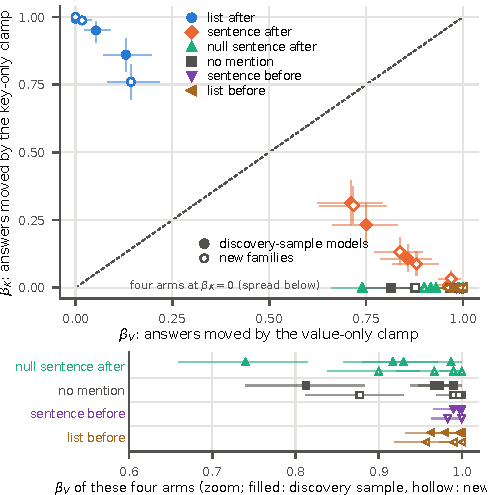
\includegraphics[width=0.8\textwidth]{figures/fig_crossover.pdf}
\caption{\textbf{Generated answers follow the channel the later mentions open} (fresh stories, eight models; the data of \cref{fig:schematic}c as a scatter). Each point is one model and arm: $\beta_K$, the share of generated answers that move to the clamped value under the key-only clamp, against $\beta_V$, the same under the value-only clamp, both net of moves to the clamped value under the clamp to the other of S and X; 95\,\% cluster intervals. The strip below spreads out the four arms whose $\beta_K$ is zero in every model (no mention, list before, sentence before, null sentence).}
\label{fig:crossover-full}
\end{figure}

\paragraph{The lines (J-B5, J-B5b).} With the list after the story, the key-only clamp moves \JbRangeBetaKAfterPfourMin{}--\JbRangeBetaKAfterPfourMax{} of generated answers to the clamped value in the discovery-sample models and \JbRangeBetaKAfterNfourMin{}--\JbRangeBetaKAfterNfourMax{} in the new families; without a mention, with the list before or with the sentence before, it moves none (\JbRangeBetaKNoneEightMax{}, \JbRangeBetaKBeforeEightMax{} and \JbRangeBetaKPreEightMax{} at most), and the value-only clamp moves \JbRangeBetaVNoneEightMin{}--\JbRangeBetaVNoneEightMax{} of answers without a mention (J-B5-P4f and J-B5-N4, held in \JbFivePfMet{} of \JbFivePfEval{} and \JbFiveNfMet{} of \JbFiveNfEval{}). The sentence read changes generated answers in seven of the eight models: the key-only clamp's flip rate is \JbFivebFlipPostMetMin{}--\JbFivebFlipPostMetMax{} after the sentence and \JbRangeFlipPreEightMax{} before it in those seven (J-B5b-N4, risky, held in \JbFivebNfMet{} of \JbFivebNfEval{}); at OLMo-2-7B the flip rate is \JbFivebFlipPostOlmoSeven{} after the sentence and \JbFivebFlipPreOlmoSeven{} before it, with a lower bound of \JbFivebLbOlmoSeven{} for the difference, so the discovery-sample line J-B5b-P4f was not met (risky; \JbFivebPfMet{} of \JbFivebPfEval{}). The record's reading (exploratory, recomputed): 3 of 150 items flip, in 3 of 55 cells, and 11.9\,\% of the resamples are exactly zero, so the failure does not depend on the seed; the key clamp under \fmtPost{} closes about 29\,\% of a 10-nat base--source margin at OLMo-2-7B, and the generations agree with the emitted-form argmax: the read is present in log-probabilities but too small to change OLMo-2's answers. The pre-written texts had no wording for this split; the wording used is a disclosed decision (\cref{app:decisions}). % verbatim: outcome J part B

\paragraph{The crossover (reported).} Over the eight models, $\beta_K$ under \fmtListA{} is \JbRangeBetaKAfterEightMin{}--\JbRangeBetaKAfterEightMax{} against $\beta_V$ = \JbRangeBetaVAfterEightMin{}--\JbRangeBetaVAfterEightMax{}; without a mention $\beta_V$ is \JbRangeBetaVNoneEightMin{}--\JbRangeBetaVNoneEightMax{} against $\beta_K$ = \JbRangeBetaKNoneEightMax{}; under \fmtPost{} $\beta_K$ is \JbRangeBetaKPostEightMin{}--\JbRangeBetaKPostEightMax{} and $\beta_V$ \JbRangeBetaVPostEightMin{}--\JbRangeBetaVPostEightMax{}; under \fmtNull{} $\beta_K$ is \JbRangeBetaKPostNullEightMax{} in every model and $\beta_V$ \JbRangeBetaVPostNullEightMin{}--\JbRangeBetaVPostNullEightMax{}. A single-channel clamp creates a cache state that no prompt produces; the generated answers show that the channel the later mentions open is the one that changes what the model says.

\subsection{Natural passages}\label{app:natural}

\paragraph{Design and gates.} Four models (Llama-3.1-8B and Gemma-2-9B, two families never examined before, and Qwen2.5-7B and Mistral-7B) answered the 185 counterfactual passages in six formats (\cref{app:prompts-natural}). Each line is decided on the items competent in its formats (the clean run answers B, the clamp to S answers S and the clamp to X answers X) and must hold in every evaluable model, with at least three evaluable models including a new family. Intervals are 95\,\% two-stage bootstrap intervals over articles and the items within them. Three gates decide evaluability (\cref{app:impl-j}). The BF16 floor failed in one cell, Llama-3.1-8B's options-after cell, by one item (generation agreement \JaGoneAgreeOptaLlamaEight{} against 0.97); every line that uses that cell is not evaluable in Llama. The competence floor of 80 items failed in five cells: Llama-3.1-8B with the related-articles sentence after and before the passage, and Mistral-7B in free form and with the sentence after and before. Mistral's free-form answers are mostly sentences (``The passage states that \ldots''), which the answer rule does not read as the entity, while its clamped answers never name B (exploratory, recomputed): a failure of answer form, not of compliance with the counterfactual. The emitted-form gate held in every cell (median probability of the decision token \JaGthreePMin{}--\JaGthreePMax{}; the first generated token was the decision token in at least \JaGthreeGoneMin{} of competent items). \Cref{tab:natural8} gives every model and format. % verbatim: outcome J part A

\begin{table}[!ht]
\centering
\caption{\textbf{Natural passages: identity by format.} Counterfactual SQuAD passages, 185 items per model; $n_{\mathrm{comp}}$: items competent in the format; $s_{\mathrm{ID}}$, $\mathrm{ID}_K$ and $\mathrm{ID}_V$ on those items, with 95\,\% two-stage article-cluster intervals. Gate: the preregistered gate that fails in the cell (J-A-G1: BF16 floor; J-A-G2: fewer than 80 competent items); such a cell enters no line. $^\dagger$Computed from the raw results with the scorer's functions, not printed by the scorer (exploratory).}
\label{tab:natural8}
\small
\setlength{\tabcolsep}{4pt}
\begin{tabular}{@{}llrcccl@{}}
\toprule
Model & Format & $n_{\mathrm{comp}}$ & $s_{\mathrm{ID}}$ & $\mathrm{ID}_K$ (nats) & $\mathrm{ID}_V$ (nats) & Gate \\
\midrule
Llama-3.1-8B & options after & 148 & \begin{tabular}[t]{@{}c@{}}0.524\\[-1pt]{\scriptsize[0.473, 0.568]}\end{tabular} & \begin{tabular}[t]{@{}c@{}}6.859\\[-1pt]{\scriptsize[5.903, 7.829]}\end{tabular} & \begin{tabular}[t]{@{}c@{}}6.237\\[-1pt]{\scriptsize[5.702, 6.805]}\end{tabular} & J-A-G1 \\
 & letters after & 156 & \begin{tabular}[t]{@{}c@{}}0.739\\[-1pt]{\scriptsize[0.675, 0.794]}\end{tabular} & \begin{tabular}[t]{@{}c@{}}6.726\\[-1pt]{\scriptsize[5.873, 7.572]}\end{tabular} & \begin{tabular}[t]{@{}c@{}}2.371\\[-1pt]{\scriptsize[1.805, 3.080]}\end{tabular} & -- \\
 & sentence after$^\dagger$ & 70 & \begin{tabular}[t]{@{}c@{}}0.075\\[-1pt]{\scriptsize[0.044, 0.106]}\end{tabular} & \begin{tabular}[t]{@{}c@{}}0.916\\[-1pt]{\scriptsize[0.514, 1.339]}\end{tabular} & \begin{tabular}[t]{@{}c@{}}11.260\\[-1pt]{\scriptsize[10.555, 11.969]}\end{tabular} & J-A-G2 \\
 & free form & 86 & \begin{tabular}[t]{@{}c@{}}0.045\\[-1pt]{\scriptsize[0.026, 0.063]}\end{tabular} & \begin{tabular}[t]{@{}c@{}}0.552\\[-1pt]{\scriptsize[0.315, 0.794]}\end{tabular} & \begin{tabular}[t]{@{}c@{}}11.786\\[-1pt]{\scriptsize[11.122, 12.434]}\end{tabular} & -- \\
 & options before$^\dagger$ & 164 & \begin{tabular}[t]{@{}c@{}}$-$0.023\\[-1pt]{\scriptsize[$-$0.035, $-$0.011]}\end{tabular} & \begin{tabular}[t]{@{}c@{}}$-$0.252\\[-1pt]{\scriptsize[$-$0.383, $-$0.121]}\end{tabular} & \begin{tabular}[t]{@{}c@{}}11.176\\[-1pt]{\scriptsize[10.440, 11.972]}\end{tabular} & -- \\
 & sentence before$^\dagger$ & 69 & \begin{tabular}[t]{@{}c@{}}$-$0.021\\[-1pt]{\scriptsize[$-$0.042, $-$0.002]}\end{tabular} & \begin{tabular}[t]{@{}c@{}}$-$0.227\\[-1pt]{\scriptsize[$-$0.429, $-$0.020]}\end{tabular} & \begin{tabular}[t]{@{}c@{}}10.784\\[-1pt]{\scriptsize[10.084, 11.531]}\end{tabular} & J-A-G2 \\
\midrule
Gemma-2-9B & options after & 158 & \begin{tabular}[t]{@{}c@{}}0.627\\[-1pt]{\scriptsize[0.599, 0.653]}\end{tabular} & \begin{tabular}[t]{@{}c@{}}9.868\\[-1pt]{\scriptsize[9.073, 10.596]}\end{tabular} & \begin{tabular}[t]{@{}c@{}}5.869\\[-1pt]{\scriptsize[5.379, 6.389]}\end{tabular} & -- \\
 & letters after & 158 & \begin{tabular}[t]{@{}c@{}}0.963\\[-1pt]{\scriptsize[0.927, 0.987]}\end{tabular} & \begin{tabular}[t]{@{}c@{}}9.676\\[-1pt]{\scriptsize[9.121, 10.128]}\end{tabular} & \begin{tabular}[t]{@{}c@{}}0.375\\[-1pt]{\scriptsize[0.132, 0.750]}\end{tabular} & -- \\
 & sentence after$^\dagger$ & 107 & \begin{tabular}[t]{@{}c@{}}0.067\\[-1pt]{\scriptsize[0.043, 0.092]}\end{tabular} & \begin{tabular}[t]{@{}c@{}}1.047\\[-1pt]{\scriptsize[0.653, 1.496]}\end{tabular} & \begin{tabular}[t]{@{}c@{}}14.685\\[-1pt]{\scriptsize[14.010, 15.349]}\end{tabular} & -- \\
 & free form & 109 & \begin{tabular}[t]{@{}c@{}}$-$0.003\\[-1pt]{\scriptsize[$-$0.010, 0.002]}\end{tabular} & \begin{tabular}[t]{@{}c@{}}$-$0.057\\[-1pt]{\scriptsize[$-$0.164, 0.037]}\end{tabular} & \begin{tabular}[t]{@{}c@{}}16.900\\[-1pt]{\scriptsize[16.204, 17.582]}\end{tabular} & -- \\
 & options before$^\dagger$ & 167 & \begin{tabular}[t]{@{}c@{}}$-$0.017\\[-1pt]{\scriptsize[$-$0.024, $-$0.011]}\end{tabular} & \begin{tabular}[t]{@{}c@{}}$-$0.183\\[-1pt]{\scriptsize[$-$0.262, $-$0.117]}\end{tabular} & \begin{tabular}[t]{@{}c@{}}11.234\\[-1pt]{\scriptsize[10.786, 11.692]}\end{tabular} & -- \\
 & sentence before$^\dagger$ & 117 & \begin{tabular}[t]{@{}c@{}}$-$0.018\\[-1pt]{\scriptsize[$-$0.024, $-$0.012]}\end{tabular} & \begin{tabular}[t]{@{}c@{}}$-$0.247\\[-1pt]{\scriptsize[$-$0.332, $-$0.164]}\end{tabular} & \begin{tabular}[t]{@{}c@{}}14.176\\[-1pt]{\scriptsize[13.500, 14.855]}\end{tabular} & -- \\
\midrule
Qwen2.5-7B & options after & 162 & \begin{tabular}[t]{@{}c@{}}0.677\\[-1pt]{\scriptsize[0.639, 0.715]}\end{tabular} & \begin{tabular}[t]{@{}c@{}}15.491\\[-1pt]{\scriptsize[13.983, 16.966]}\end{tabular} & \begin{tabular}[t]{@{}c@{}}7.385\\[-1pt]{\scriptsize[6.287, 8.550]}\end{tabular} & -- \\
 & letters after & 163 & \begin{tabular}[t]{@{}c@{}}0.935\\[-1pt]{\scriptsize[0.885, 0.972]}\end{tabular} & \begin{tabular}[t]{@{}c@{}}19.782\\[-1pt]{\scriptsize[18.416, 20.972]}\end{tabular} & \begin{tabular}[t]{@{}c@{}}1.366\\[-1pt]{\scriptsize[0.591, 2.438]}\end{tabular} & -- \\
 & sentence after$^\dagger$ & 106 & \begin{tabular}[t]{@{}c@{}}0.061\\[-1pt]{\scriptsize[0.027, 0.096]}\end{tabular} & \begin{tabular}[t]{@{}c@{}}1.335\\[-1pt]{\scriptsize[0.564, 2.144]}\end{tabular} & \begin{tabular}[t]{@{}c@{}}20.573\\[-1pt]{\scriptsize[19.205, 21.983]}\end{tabular} & -- \\
 & free form & 104 & \begin{tabular}[t]{@{}c@{}}0.014\\[-1pt]{\scriptsize[0.004, 0.025]}\end{tabular} & \begin{tabular}[t]{@{}c@{}}0.311\\[-1pt]{\scriptsize[0.081, 0.548]}\end{tabular} & \begin{tabular}[t]{@{}c@{}}21.430\\[-1pt]{\scriptsize[20.006, 22.911]}\end{tabular} & -- \\
 & options before$^\dagger$ & 166 & \begin{tabular}[t]{@{}c@{}}$-$0.053\\[-1pt]{\scriptsize[$-$0.067, $-$0.041]}\end{tabular} & \begin{tabular}[t]{@{}c@{}}$-$0.878\\[-1pt]{\scriptsize[$-$1.087, $-$0.671]}\end{tabular} & \begin{tabular}[t]{@{}c@{}}17.310\\[-1pt]{\scriptsize[16.163, 18.440]}\end{tabular} & -- \\
 & sentence before$^\dagger$ & 99 & \begin{tabular}[t]{@{}c@{}}$-$0.036\\[-1pt]{\scriptsize[$-$0.051, $-$0.022]}\end{tabular} & \begin{tabular}[t]{@{}c@{}}$-$0.725\\[-1pt]{\scriptsize[$-$0.993, $-$0.454]}\end{tabular} & \begin{tabular}[t]{@{}c@{}}20.770\\[-1pt]{\scriptsize[19.338, 22.218]}\end{tabular} & -- \\
\midrule
Mistral-7B & options after & 157 & \begin{tabular}[t]{@{}c@{}}0.550\\[-1pt]{\scriptsize[0.503, 0.593]}\end{tabular} & \begin{tabular}[t]{@{}c@{}}9.817\\[-1pt]{\scriptsize[8.568, 11.071]}\end{tabular} & \begin{tabular}[t]{@{}c@{}}8.029\\[-1pt]{\scriptsize[7.187, 8.907]}\end{tabular} & -- \\
 & letters after & 155 & \begin{tabular}[t]{@{}c@{}}0.786\\[-1pt]{\scriptsize[0.701, 0.864]}\end{tabular} & \begin{tabular}[t]{@{}c@{}}7.424\\[-1pt]{\scriptsize[6.211, 8.638]}\end{tabular} & \begin{tabular}[t]{@{}c@{}}2.016\\[-1pt]{\scriptsize[1.219, 2.987]}\end{tabular} & -- \\
 & sentence after$^\dagger$ & 43 & \begin{tabular}[t]{@{}c@{}}0.092\\[-1pt]{\scriptsize[0.009, 0.168]}\end{tabular} & \begin{tabular}[t]{@{}c@{}}1.545\\[-1pt]{\scriptsize[0.139, 3.045]}\end{tabular} & \begin{tabular}[t]{@{}c@{}}15.330\\[-1pt]{\scriptsize[14.205, 16.444]}\end{tabular} & J-A-G2 \\
 & free form & 43 & \begin{tabular}[t]{@{}c@{}}0.001\\[-1pt]{\scriptsize[$-$0.011, 0.015]}\end{tabular} & \begin{tabular}[t]{@{}c@{}}0.019\\[-1pt]{\scriptsize[$-$0.184, 0.257]}\end{tabular} & \begin{tabular}[t]{@{}c@{}}16.426\\[-1pt]{\scriptsize[15.215, 17.516]}\end{tabular} & J-A-G2 \\
 & options before$^\dagger$ & 150 & \begin{tabular}[t]{@{}c@{}}$-$0.026\\[-1pt]{\scriptsize[$-$0.037, $-$0.016]}\end{tabular} & \begin{tabular}[t]{@{}c@{}}$-$0.387\\[-1pt]{\scriptsize[$-$0.540, $-$0.240]}\end{tabular} & \begin{tabular}[t]{@{}c@{}}15.195\\[-1pt]{\scriptsize[14.444, 15.971]}\end{tabular} & -- \\
 & sentence before$^\dagger$ & 44 & \begin{tabular}[t]{@{}c@{}}$-$0.018\\[-1pt]{\scriptsize[$-$0.040, 0.000]}\end{tabular} & \begin{tabular}[t]{@{}c@{}}$-$0.278\\[-1pt]{\scriptsize[$-$0.586, 0.004]}\end{tabular} & \begin{tabular}[t]{@{}c@{}}15.313\\[-1pt]{\scriptsize[14.206, 16.307]}\end{tabular} & J-A-G2 \\
\bottomrule
\end{tabular}

\end{table}

\paragraph{Identity (J-A1--J-A5).} With options after the passage the key carries most of the answer entity's identity in the three evaluable models (J-A1, extrapolation, held: $s_{\mathrm{ID}}$ \JaSidOptaGemmaNine{}, \JaSidOptaQwenSeven{} and \JaSidOptaMistralSeven{} at Gemma-2-9B, Qwen2.5-7B and Mistral-7B, lower bounds above the preregistered 0.35; Llama-3.1-8B's cell, \JaSidOptaLlamaEight{}, not evaluable), also for answers of three or more tokens (J-A1b, risky, held: \JaOnebSidGemmaNine{} [\JaOnebSidGemmaNineLo{}, \JaOnebSidGemmaNineHi{}], \JaOnebSidQwenSeven{} [\JaOnebSidQwenSevenLo{}, \JaOnebSidQwenSevenHi{}] and \JaOnebSidMistralSeven{} [\JaOnebSidMistralSevenLo{}, \JaOnebSidMistralSevenHi{}]), and with lettered options in all four (J-A1c, held: $s_{\mathrm{ID}}$ \JaSidLetaLlamaEight{}--\JaSidLetaGemmaNine{}). In free form the value carries it (J-A2, held: $s_{\mathrm{ID}}$ \JaSidNomLlamaEight{}, \JaSidNomGemmaNine{} and \JaSidNomQwenSeven{} at Llama, Gemma and Qwen; Mistral not evaluable). The derived contrast J-A3 (options after minus free form at least 0.4; not counted) holds in both models where it is evaluable (\JaThreeDiffGemmaNine{} and \JaThreeDiffQwenSeven{}) and is not evaluable, because Llama's options-after cell and Mistral's free-form cell fail their gates. Options before the passage give a small negative key read in every model (J-A4, replication, held: $\mathrm{ID}_K$ \JaFourIDKOptbMin{} to \JaFourIDKOptbMax{} nats, ratios to the options-after read \JaFourRatioMin{} to \JaFourRatioMax{}); the line's criteria are one-sided. A related-articles sentence after the passage opens only a small key read: its gain in $s_{\mathrm{ID}}$ over free form is \JaFiveDiffGemmaNine{} at Gemma and \JaFiveDiffQwenSeven{} at Qwen, below the preregistered 0.10 (J-A5, risky, not held; Llama and Mistral not evaluable), although its key read is positive (\cref{tab:natural8}). Its contrast with the same sentence before the passage, J-A5B, holds in both evaluable models ($\mathrm{ID}_K$ difference \JaFiveBDiffGemmaNine{} and \JaFiveBDiffQwenSeven{} nats) and is not evaluable (two of the three required models).

\begin{table}[!ht]
\centering
\footnotesize
\caption{\textbf{Cue conflict and the copy fallback on passages.} The cache gets two sources: the key from one counterfactual entity and the value from another (S and X, both directions). Key / value: the share of generated answers naming the key's or the value's entity; ``other'': answers naming no candidate; dec.: the value-source rate at the decision token alone. Flag only: the key from S and the value from a third entity Z, share answering S; copy fallback: the key from Z and the value from S, share answering S. Whole answers; competent items; cells of Llama's options-after and Mistral's free-form formats fail a gate (not evaluable).}
\label{tab:cue}
\setlength{\tabcolsep}{4pt}
\begin{tabular}{@{}lccccccccc@{}}
\toprule
 & \multicolumn{2}{c}{options after} & \multicolumn{2}{c}{lettered options} & \multicolumn{3}{c}{free form} & flag only & copy fallback \\
\cmidrule(lr){2-3}\cmidrule(lr){4-5}\cmidrule(lr){6-8}
Model & key & value & key & value & value & other & value (dec.) & (options after) & (options after) \\
\midrule
Llama-3.1-8B & \JaKeySrcOptaLlamaEight{} & \JaValSrcOptaLlamaEight{} & \JaKeySrcLetaLlamaEight{} & \JaValSrcLetaLlamaEight{} & \JaValSrcNomLlamaEight{} & \JaOtherNomLlamaEight{} & \JaValSrcDecNomLlamaEight{} & \JaSixdOptaLlamaEight{} & \JaSixeSLlamaEight{} \\
Gemma-2-9B & \JaKeySrcOptaGemmaNine{} & \JaValSrcOptaGemmaNine{} & \JaKeySrcLetaGemmaNine{} & \JaValSrcLetaGemmaNine{} & \JaValSrcNomGemmaNine{} & \JaOtherNomGemmaNine{} & \JaValSrcDecNomGemmaNine{} & \JaSixdOptaGemmaNine{} & \JaSixeSGemmaNine{} \\
Qwen2.5-7B & \JaKeySrcOptaQwenSeven{} & \JaValSrcOptaQwenSeven{} & \JaKeySrcLetaQwenSeven{} & \JaValSrcLetaQwenSeven{} & \JaValSrcNomQwenSeven{} & \JaOtherNomQwenSeven{} & \JaValSrcDecNomQwenSeven{} & \JaSixdOptaQwenSeven{} & \JaSixeSQwenSeven{} \\
Mistral-7B & \JaKeySrcOptaMistralSeven{} & \JaValSrcOptaMistralSeven{} & \JaKeySrcLetaMistralSeven{} & \JaValSrcLetaMistralSeven{} & \JaValSrcNomMistralSeven{} & \JaOtherNomMistralSeven{} & \JaValSrcDecNomMistralSeven{} & \JaSixdOptaMistralSeven{} & \JaSixeSMistralSeven{} \\
\bottomrule
\end{tabular}
\end{table}

\paragraph{Behaviour (J-A6a--e).} \Cref{tab:cue} gives the cue-conflict rates. With lettered options the generated answer follows the key's entity in all four models (J-A6b, risky, held), and when the key matches no option the value is copied (J-A6e, risky, held in the three evaluable models). With options answered by name the key wins at Gemma and Qwen but not at Mistral (key-source rate \JaKeySrcOptaMistralSeven{} against the preregistered 0.6; J-A6a, risky, not held). In free form the value-source rate misses 0.6 at Llama and Qwen (J-A6c, risky, not held; Mistral not evaluable): many of the answers that name no candidate are hybrids that start with the value source's first word and do not complete the entity (34\,\% of the ``other'' answers at Llama to 76\,\% at Gemma; recomputed), and at the decision token the value-source rate is \JaValSrcDecNomMin{}--\JaValSrcDecNomMax{} while the key-source rate is at most 0.005. Scored on the answer's first word, which is not the preregistered criterion, the value-source rates would be 0.674 / 0.950 / 0.740 / 0.547 (Llama / Gemma / Qwen / Mistral; Llama's lower bound 0.55, exploratory, recomputed) and J-A6c would be met; as preregistered (the whole answer) it is not. The key-only flag (J-A6d) moves answers to the key's entity with options after the passage and never in free form in every model, but the line is not evaluable (two evaluable models). Llama's options-after cue conflict, whose cell is not evaluable, favours the value (key \JaKeySrcOptaLlamaEight{}, value \JaValSrcOptaLlamaEight{}), driven by numbers, 67 of its 70 single-token items, and by person names whose tokens are split between the key and the value source (exploratory, recomputed). Because J-A6a and J-A6c both failed, the hybrids are reported as an observation, not under the pre-written clause for a failure of J-A6c alone (\cref{app:decisions}), and the channel attributions are not shown to decide behaviour on natural text. % verbatim: outcome J part A

\paragraph{Continuations (J-A8, not evaluable; J-A8d, not held).} The continuation of a multi-token answer is read through an interaction of the two channels in all four models: in free form, the key and value effects on the continuation tokens add up to far less than the joint effect ($I_{\mathrm{cont}}$ = \JaIcontMin{}--\JaIcontMax{}), while at the decision token they add up ($I_{\mathrm{dec}}$ = \JaIdecMin{} to \JaIdecMax{}), and with options listed the joint clamp hardly moves the continuation (\JaContRatioMin{}--\JaContRatioMax{} of its free-form effect). The key alone moves the continuation away from S ($d_K^{\mathrm{cont}}$ = \JaDcontKMin{} to \JaDcontKMax{} nats), the pattern the line predicted: the key addresses the next piece and the value supplies it. This pattern is seen in all four models, but its line (J-A8, extrapolation) is not evaluable (two evaluable models: Llama's options-after cell fails the BF16 gate and Mistral's free-form cell the competence gate); it is a channel-level replication of induction-head K-composition \citep{elhage2021framework,olsson2022context}, not a novelty claim. The hybrid rate under a key that matches no candidate (J-A8d, risky) rests on Gemma alone, the one model with enough items (\JaEightdNomGemmaNine{} [\JaEightdNomGemmaNineLo{}, \JaEightdNomGemmaNineHi{}], 6 of 57 items, against 0.2), many of whose B entities are famous names that the model completes from memory; not held. % verbatim: outcome J part A

\paragraph{Quantization of the cached values (J-A7, J-A7b; exploratory reading).} The passage part also tested whether quantizing the passage's cached values to 2 bits with KIVI \citep{liu2024kivi} hurts free-form answers more than multiple-choice ones, beyond the same quantization of the keys. Only Qwen2.5-7B had enough prior-free items (33): the difference in differences was \JaSevenDiDQwenSeven{} [\JaSevenDiDQwenSevenLo{}, \JaSevenDiDQwenSevenHi{}] (J-A7, risky, not held) and the value drop's difference between formats \JaSevenbDiffQwenSeven{} [\JaSevenbDiffQwenSevenLo{}, \JaSevenbDiffQwenSevenHi{}] (J-A7b, risky, not held). The test had low power (the drops come from four and one items) and points the other way: on all competent items 2-bit keys cost free-form answers more than 2-bit values do (\cref{tab:kivi}), and neither costs multiple-choice answers (accuracy at least \JaKiviMcqMin{}). The relative reconstruction errors are \JaKiviErrKMin{}--\JaKiviErrKMax{} for the keys (per channel) and \JaKiviErrVMin{}--\JaKiviErrVMax{} for the values (per token), without strength matching. We make no claim about quantization. % verbatim: 33 items, outcome J part A

\begin{table}[!ht]
\centering
\footnotesize
\caption{\textbf{KIVI 2-bit quantization of the passage's cache} (exploratory). Faithful accuracy (the generation names S on the S passage) on competent items with no quantization, with 2-bit keys and with 2-bit values (every passage token, every layer; keys per channel, values per token, groups of 32), and the relative reconstruction errors $\lVert x' - x \rVert / \lVert x \rVert$.}
\label{tab:kivi}
\setlength{\tabcolsep}{5pt}
\begin{tabular}{@{}llccccc@{}}
\toprule
Model & Format & none & keys 2-bit & values 2-bit & error (keys) & error (values) \\
\midrule
Llama-3.1-8B & free form & \JaKiviNoneNomLlamaEight{} & \JaKiviKtwoNomLlamaEight{} & \JaKiviVtwoNomLlamaEight{} & \JaKiviErrKNomLlamaEight{} & \JaKiviErrVNomLlamaEight{} \\
 & options after & \JaKiviNoneOptaLlamaEight{} & \JaKiviKtwoOptaLlamaEight{} & \JaKiviVtwoOptaLlamaEight{} & \JaKiviErrKOptaLlamaEight{} & \JaKiviErrVOptaLlamaEight{} \\
 & lettered options & \JaKiviNoneLetaLlamaEight{} & \JaKiviKtwoLetaLlamaEight{} & \JaKiviVtwoLetaLlamaEight{} & \JaKiviErrKLetaLlamaEight{} & \JaKiviErrVLetaLlamaEight{} \\
\addlinespace[2pt]
Gemma-2-9B & free form & \JaKiviNoneNomGemmaNine{} & \JaKiviKtwoNomGemmaNine{} & \JaKiviVtwoNomGemmaNine{} & \JaKiviErrKNomGemmaNine{} & \JaKiviErrVNomGemmaNine{} \\
 & options after & \JaKiviNoneOptaGemmaNine{} & \JaKiviKtwoOptaGemmaNine{} & \JaKiviVtwoOptaGemmaNine{} & \JaKiviErrKOptaGemmaNine{} & \JaKiviErrVOptaGemmaNine{} \\
 & lettered options & \JaKiviNoneLetaGemmaNine{} & \JaKiviKtwoLetaGemmaNine{} & \JaKiviVtwoLetaGemmaNine{} & \JaKiviErrKLetaGemmaNine{} & \JaKiviErrVLetaGemmaNine{} \\
\addlinespace[2pt]
Qwen2.5-7B & free form & \JaKiviNoneNomQwenSeven{} & \JaKiviKtwoNomQwenSeven{} & \JaKiviVtwoNomQwenSeven{} & \JaKiviErrKNomQwenSeven{} & \JaKiviErrVNomQwenSeven{} \\
 & options after & \JaKiviNoneOptaQwenSeven{} & \JaKiviKtwoOptaQwenSeven{} & \JaKiviVtwoOptaQwenSeven{} & \JaKiviErrKOptaQwenSeven{} & \JaKiviErrVOptaQwenSeven{} \\
 & lettered options & \JaKiviNoneLetaQwenSeven{} & \JaKiviKtwoLetaQwenSeven{} & \JaKiviVtwoLetaQwenSeven{} & \JaKiviErrKLetaQwenSeven{} & \JaKiviErrVLetaQwenSeven{} \\
\addlinespace[2pt]
Mistral-7B & free form & \JaKiviNoneNomMistralSeven{} & \JaKiviKtwoNomMistralSeven{} & \JaKiviVtwoNomMistralSeven{} & \JaKiviErrKNomMistralSeven{} & \JaKiviErrVNomMistralSeven{} \\
 & options after & \JaKiviNoneOptaMistralSeven{} & \JaKiviKtwoOptaMistralSeven{} & \JaKiviVtwoOptaMistralSeven{} & \JaKiviErrKOptaMistralSeven{} & \JaKiviErrVOptaMistralSeven{} \\
 & lettered options & \JaKiviNoneLetaMistralSeven{} & \JaKiviKtwoLetaMistralSeven{} & \JaKiviVtwoLetaMistralSeven{} & \JaKiviErrKLetaMistralSeven{} & \JaKiviErrVLetaMistralSeven{} \\
\bottomrule
\end{tabular}
\end{table}

\paragraph{Reader heads on passages (J-A-HA1--HA3b, not evaluable).} The head lines needed Qwen2.5-7B and Mistral-7B. At Qwen2.5-7B the heads' BF16 floor failed ($\lvert m(\text{none}) - m(\text{clean})\rvert$ = \JaHaGoneNoneCleanQwenSeven{} nats against \JaHaGoneBoundQwenSeven{}): plain eager passes in different batch shapes differ by 0.7--0.9 nats at Qwen (0.1 at Mistral), and Qwen's eager teacher-forced chain fails in most items whose continuation contains the digit ``0'' (exploratory, recomputed), so every head line is not evaluable. The option rows are the readers in both models ($d_G/d_{\mathrm{full}}$ = \JaHaGtwoRatioQwenSeven{} and \JaHaGtwoRatioMistralSeven{}). At Mistral-7B, whose gates passed (exploratory): the top \JaHaKstarMistralSeven{} heads ranked on the passages recover $R$ = \JaHaOneRMistralSeven{} of the option rows' read and blinding them removes \JaHaOneKOMistralSeven{}, against \JaHaOneRrandMistralSeven{} and \JaHaOneKOrandMistralSeven{} for random sets; the reader heads found on the templated stories recover \JaHaTwoRMistralSeven{} and remove \JaHaTwoKOMistralSeven{} (\JaHaTwoOverlapMistralSeven{} heads shared with the natural set); and mean-ablating the natural set at every row after the question lowers faithful multiple-choice accuracy on prior-free items by \JaHaThreeaDropMistralSeven{}. Ablating the heads with the largest direct effect on the answer in free form (a copy set) breaks both formats (faithful accuracy with options after \JaAblFaithNoneOptaQwenSeven{} $\to$ \JaAblFaithCstarOptaQwenSeven{} at Qwen and \JaAblFaithNoneOptaMistralSeven{} $\to$ \JaAblFaithCstarOptaMistralSeven{} at Mistral; in free form \JaAblFaithNoneNomQwenSeven{} $\to$ \JaAblFaithCstarNomQwenSeven{} and \JaAblFaithNoneNomMistralSeven{} $\to$ \JaAblFaithCstarNomMistralSeven{}), and ablating the natural readers also lowers free-form accuracy (to \JaAblFaithNstarNomQwenSeven{} and \JaAblFaithNstarNomMistralSeven{}; exploratory): the readers found at the option rows are needed for free-form answers as well. Because ablating the readers and cutting their attention disagree on whether the copy route takes over in the discovery sample (\cref{app:heads}), these passage tests would have bridged the two; they are not evaluable. % verbatim: outcome J part A

\paragraph{Sensitivity: Llama's options-after cell (disclosed).} Had the BF16 gate passed in that cell (180 of 185 items instead of 179), J-A3 would be met (three evaluable models including a new family) and J-A6d not met (Llama's flag-only rate \JaSixdOptaLlamaEight{} against 0.6); J-A1, J-A4, J-A6a and J-A6e would not change, and the risky tally of this part would read 3 of 10 (expected 4.65). % verbatim: outcome J part A

\paragraph{Holm sensitivity.} Over the 43 interval components of this part's risky lines, Holm's step-down changes one decision, J-A5's component at Qwen2.5-7B ($p$ = \JaHolmP{} against a threshold of \JaHolmThr{}), and no verdict. J-A6b's Mistral component passes Holm by a relative margin of 0.2\,\% ($p$ 0.002772 against 0.002778), within the Monte Carlo error of the bootstrap standard error, so J-A6b should not be described as robust to Holm. % verbatim: outcome J part A

\paragraph{Reported and exploratory.} Without the passage, the question and options alone favour the original answer: the closed-book argmax is $e_B$ in \JaPriorOptMin{}--\JaPriorOptMax{} of items (persons \JaPriorOptPersonMin{}--\JaPriorOptPersonMax{}, numbers \JaPriorOptNumberMin{}--\JaPriorOptNumberMax{}); the identity measures are contrasts between S and X, from which this prior cancels to first order. On all 185 valid items (not only competent ones) the pattern is the same: $s_{\mathrm{ID}}$ with the sentence after the passage is \JaSidAllMenaMin{}--\JaSidAllMenaMax{}, and with options or the sentence before it \JaSidAllBeforeMin{} to \JaSidAllBeforeMax{}; the option mass at the decision token is \JaMassAllListMin{}--\JaMassAllListMax{} with the options listed and \JaMassAllNoListMin{}--\JaMassAllNoListMax{} without. In the LEAK stratum (a surname re-mentioned in the passage after the full name; 65 items) $s_{\mathrm{ID}}$ is \JaLeakSidNomMin{}--\JaLeakSidNomMax{} in free form and \JaLeakSidOptaMin{}--\JaLeakSidOptaMax{} with options after. This says nothing about whether a natural in-passage re-mention opens a key read: the S, X and Z passages differ from B only inside the answer span, so the re-mention still names the original entity, and its match to a foreign key is lost alike under S and X and cancels in the S-versus-X contrast of \cref{eq:idk}. A test needs the counterfactual written at every mention (\cref{sec:limitations}, (i)). On years (80 items), at the first digit that differs, the free-form read is value-only ($d_K$ \JaEfourDKNomMin{} to \JaEfourDKNomMax{} nats against $d_V$ \JaEfourDVNomMin{}--\JaEfourDVNomMax{}), and with options listed the key reads ($d_K$ \JaEfourDKOptaMin{}--\JaEfourDKOptaMax{}), against the written expectation, which was value-only for both formats. Scored on the full answer string from the decision token on, $s_{\mathrm{ID}}$ in free form is negative (\JaEsixSidNomMin{} to \JaEsixSidNomMax{}), the continuation pattern above. With the clamp started at 30\,\% of the depth the free-form value copy keeps \JaEoneOnNomMin{}--\JaEoneOnNomMax{} of its full effect, while the options-after key read keeps \JaEoneOnOptaMin{}--\JaEoneOnOptaMax{}; the first span piece carries \JaEoneFirstNomMin{}--\JaEoneFirstNomMax{} of the value copy, while the later pieces carry \JaEoneRestOptaMin{}--\JaEoneRestOptaMax{} of the key read (the first \JaEoneFirstOptaMin{}--\JaEoneFirstOptaMax{}). All of these are exploratory. % verbatim: 65 and 80 items, entry J part A

\clearpage
% Appendix E: details of Claim 2 (a match at the later mention, read by key). Input by sections/appendix.tex.
\section{A match at the later mention, read by key: details}\label{app:claim2}

This appendix gives the discovery-sample results on which later tokens read the writing token's key and through which heads (\cref{app:readers,app:heads}; preregistrations D, G and H), and the final round's tests of what those heads write (\cref{app:flag}), what sets the sign of the read (\cref{app:sign}) and how the flag behaves across scale (\cref{app:scale}). The final round's mechanism tests use Qwen2.5-7B and Mistral-7B (and Qwen2.5-1.5B and 3B for scale), the reader heads frozen from the discovery sample, flags fit on its 60 ranking stories and 100 new evaluation stories; intervals are 95\,\% story-bootstrap intervals, and a line over the two 7B models holds only if it holds in both.

\subsection{The mechanism tests in brief}\label{app:claim2-brief}

This subsection gives, verbatim, the fuller account of the mechanism tests that the reporting plan placed in the main text (moved here; \cref{sec:claim2} gives a shorter one; the move is disclosed in \cref{app:decisions}, deviation (iv)). The status marks are those of the main text (\cref{sec:method}); the subsections below give every number.

\textbf{In two 7B models (Qwen2.5-7B, Mistral-7B), the reader heads, enriched for duplicate-token heads (discovery sample), match the writing token's key at the later mention of the written value and write a flag into that mention's row, which the answer reads by key.} The flag suffices to move the answer but is neither specific nor the only carrier, and the question sets the sign of the read.

\paragraph{Two hops.}
In the discovery sample, 5\,\% of heads, the \emph{reader heads}, read the writing token's key at the option words (hop~1): seeing the clamped key alone, they recover \HoneRQwenSeven{} and \HoneRMistralSeven{} of the option rows' read, random sets almost none, and no single head or layer carries most of the read (\cref{app:heads}). They are enriched for duplicate-token heads \citep{wang2022ioi}: the \HfourKCQwenSeven{} and \HfourKCMistralSeven{} heads carrying 80\,\% of the read have median duplicate-token scores of \HfourDQwenSeven{} and \HfourDMistralSeven{}, against \HfourDwholeQwenSeven{} and \HfourDwholeMistralSeven{} over all heads (exploratory), a core that depends on how many heads are counted. Mean-ablating all reader heads at the option rows leaves \HthreeRhoQwenSeven{} and \HthreeRhoMistralSeven{} of the key read and raises the value read: a copy route stays available (\cref{app:heads}). The answer reads the option words, not the writing token (hop~2), mainly by key.

\paragraph{What the readers write.}
The reader heads write one vector per layer into the re-mentioned word's row. We call it the \emph{flag}. Injected with no key clamp into the row of an option absent from the story, a version fit without that word moves the answer there (\JdOneRatioQwenSeven{} / \JdOneRatioMistralSeven{} of the key read's identity effect; the answer changes in \pct{\JdOnePiXQwenSeven} / \pct{\JdOnePiXMistralSeven} of stories)\rsk. Like the natural key clamp, the injection adds the flag at that row and removes it at the base value's row; added alone, one flag moves the answer less than the natural clamp, half a flag almost not at all (exploratory; \cref{fig:flag}a). Its mean direction names no candidate: fit under the key-only clamp or from the natural source run, it is the same direction with the same effect, although each story's write also carries its word (exploratory; \cref{app:flag}). The answer reads it by key, as it reads the natural one (giving only the answer row the option rows' original keys removes \JdFourKQwenSeven{} / \JdFourKMistralSeven{} of its effect, their original values \JdFourVQwenSeven{} / \JdFourVMistralSeven{}). But the prediction\rsk{} that it is specific failed against structured controls: at Qwen2.5-7B the mean reader output moves the answer \JdTwoRatioMeanHQwenSeven{} as much as the flag, and at Mistral-7B the story's own write with its flag component removed, norm-matched, \JdTwoRatioOrthMistralSeven{} as much (the mean output contains the flag by construction, post hoc; \cref{app:flag}). And one direction per layer does not carry the key read ($\rho_K$ = \JdThreeRhoFlagQwenSeven{} / \JdThreeRhoFlagMistralSeven{}): other carriers exist; the flag is sufficient but not necessary (\cref{fig:flag}b). Removing the flag direction leaves about half of the key read in both models, as the prediction\rsk{} allowed; it failed on its controls: at Qwen the control directions, which overlap the flag, also remove 31\,\% and 44\,\%, and ablating the whole heads removes far more (above), so the flag is not the only carrier (\cref{app:decisions}). % verbatim: outcome J part D

\paragraph{The sign of the read.}
Asked which option was \emph{not} mentioned, both reads turn negative ($\mathrm{ID}_K$ $\fpeval{round(\JdSevenQoutQwenSeven,1)}$ and $\fpeval{round(\JdSevenQoutMistralSeven,1)}$ nats), and the same frozen reader heads carry the reads under both questions (\cref{app:sign}); the flag fit with the belief question, injected under this one, reproduces its negative effect (exploratory), so the sign is applied after the first hop. In indirect-object identification (IOI) with the names re-mentioned in a parenthesis, the key read is negative and the value read positive in both models (\cref{fig:flag}c). The negative IOI read is applied at the answer's key read of the listed names (restoring their keys and values for the answer row alone removes \JdRouteKVQwenSeven{} / \JdRouteKVMistralSeven{} of it, their keys alone \JdRouteKQwenSeven{} / \JdRouteKMistralSeven{}, their values alone \JdRouteVQwenSeven{} / \JdRouteVMistralSeven{})\rsk. The prediction\rsk{} that the ten answer-side heads ranked as the flag's top readers in lists apply it failed: a different (or a distributed) reader applies the negative read (the scoring script's reading: ``different reader''), though even in lists these ten carry only part of hop~2. That the belief readers carry the IOI read\rsk{} was met at Qwen2.5-7B and is not evaluable at Mistral-7B. The flag is written in sentences as in lists at 1.5B--7B, but four further predictions\rsk{} did not hold: that it carries the size of the sentence read across scale and is read by value at 1.5B (the preregistered decision table gives ``Mixed.''; post hoc, on a contrast specific to the absent option, the injected flag reproduces the natural ratio; \cref{app:scale}), that the initial-state flag carries binding separably from order, and that a key naming no candidate acts as removing the base value's flag.

\subsection{Which later tokens read, and what a re-mention must be}\label{app:readers}\label{sec:readers}\label{sec:forms}\label{app:stage5}

Letting only the option words see the source key recovers \locScaleOptMin{}--\locScaleOptMax{} of the full key effect at 7--14B under \fmtOpt{}, and every other group at most \locScaleOptOtherMax{}; under \fmtPost{} the sentence's candidate words recover \locScalePostMin{}--\locScalePostMax{} (D3, met; \cref{fig:readers}a). Conversely, forbidding the six candidate words to attend to the writing token removes the key identity ($r_K$, the fraction left, is $\GfiveRKMin$ to \GfiveRKMax{} in 9/9 format--model cells; G5, met), and cutting a matched control column does not (G6, met). The words must name the candidates at stake: listing B with two other candidates instead of S and X gives no read (G9, met). In lists two named candidates suffice (G10, met for lists); in sentences the read grows with the number named (G10, not met for sentences), and with only S and X named the words carry \GtwelveStwoQwenFourteen{}--\GtwelveStwoQwenSeven{} of the splice effect, most of it not identity-specific (G12, not met; \cref{app:g-membership}). The candidate words are thus the main readers in lists and in sentences naming at least three candidates.

\paragraph{What a re-mention must be.} Varying the re-mentions of \fmtPost{} in four 7--14B models shows a read of the word form, largely up to case ($r_K$: $\mathrm{ID}_K$ relative to an exact repeat). Capitalised and upper-case forms read nearly fully (\GfourteenCaseMin{}--\GfourteenCaseMax{}; G14, which predicted at most 0.75, not met), but a modified noun phrase such as ``wooden shelf'' reads only partly (\GthirteenModifMin{}--\GthirteenModifMax{}; G13, not met). Synonyms and mixed-language translations carry little on our English-scored measure (at most \GfifteenRKMax{}; G15, met). No preregistered token or concept outcome holds (G16, not met). Where the read is lost, the value identity rises (G17, met), but no more than after a sentence naming other words (exploratory; \cref{app:g-forms}).

\paragraph{Localisation.} \Cref{tab:localisation} gives the row-restricted splice for each token group. The later-mention words are the listed options under \fmtOpt{} and \fmtLetter{}, and the candidate words of the neutral sentence under \fmtPost{}. Under \fmtOpt{}, the question, the story after the writing token and the remaining tokens, including the answer position, each recover at most \locScaleOptOtherMax{} at 7--14B. Under \fmtPost{} the ``other later tokens'' recover \locScalePostOtherMin{}--\locScalePostOtherMax{}, and \locScalePostLeftMin{}--\locScalePostLeftMax{} of the effect is recovered by no single group, so the groups do not add up. At Mistral-Small-24B, with the key clamped from block~6, the option rows carry \IgtwoRatioOpt{}, \IgtwoRatioLetter{} and \IgtwoRatioPost{} of the key effect under \fmtOpt{}, \fmtLetter{} and \fmtPost{} (Gate I-G2, a head splice over all heads; \cref{app:stage7}); we did not localise the read at 72B. An earlier exploratory run at Qwen2.5-1.5B gives the same picture: the option words recover \locOptChoicewords{} of the key effect under \fmtOpt{} and \locLetterChoicewords{} under \fmtLetter{}. Restricting the splice further, the read is concentrated in layers 4--15 of 28, and one of the two KV groups carries most of it (exploratory; \cref{tab:windows}).

\begin{table}[!ht]
\centering
\caption{\textbf{Which later tokens read the writing token's key.} Fraction of the full key effect (all tokens see the source key, in every layer) recovered when only one group of later tokens sees it; ratio of mean log-odds changes. ``Other later tokens'' covers the instruction, chat template, prefill and answer position. Qwen2.5-7B, Qwen2.5-14B and Mistral-7B: BF16, $n = 60$ stories per format; preregistration D (D3) for \fmtOpt{} and \fmtPost{}, \fmtLetter{} exploratory. Qwen2.5-1.5B: FP32, $n = 40$, exploratory. 95\% bootstrap CIs. The groups need not add up to one.}
\label{tab:localisation}
{\small\begin{tabular}{llcccc}
\toprule
Model & Format & later-mention words & question & story after writing token & other later tokens \\
\midrule
Qwen2.5-1.5B & \fmtOpt{} & \begin{tabular}[t]{@{}c@{}}+0.87\\[-1pt]{\scriptsize[+0.80, +0.95]}\end{tabular} & \begin{tabular}[t]{@{}c@{}}0.00\\[-1pt]{\scriptsize[$-$0.01, +0.01]}\end{tabular} & \begin{tabular}[t]{@{}c@{}}$-$0.01\\[-1pt]{\scriptsize[$-$0.01, 0.00]}\end{tabular} & \begin{tabular}[t]{@{}c@{}}0.00\\[-1pt]{\scriptsize[$-$0.04, +0.03]}\end{tabular} \\
Qwen2.5-1.5B & \fmtLetter{} & \begin{tabular}[t]{@{}c@{}}+0.98\\[-1pt]{\scriptsize[+0.96, +1.00]}\end{tabular} & \begin{tabular}[t]{@{}c@{}}+0.01\\[-1pt]{\scriptsize[0.00, +0.01]}\end{tabular} & \begin{tabular}[t]{@{}c@{}}0.00\\[-1pt]{\scriptsize[$-$0.01, 0.00]}\end{tabular} & \begin{tabular}[t]{@{}c@{}}0.00\\[-1pt]{\scriptsize[0.00, 0.00]}\end{tabular} \\
\midrule
Qwen2.5-7B & \fmtOpt{} & \begin{tabular}[t]{@{}c@{}}+0.92\\[-1pt]{\scriptsize[+0.90, +0.94]}\end{tabular} & \begin{tabular}[t]{@{}c@{}}0.00\\[-1pt]{\scriptsize[0.00, 0.00]}\end{tabular} & \begin{tabular}[t]{@{}c@{}}0.00\\[-1pt]{\scriptsize[0.00, 0.00]}\end{tabular} & \begin{tabular}[t]{@{}c@{}}+0.01\\[-1pt]{\scriptsize[+0.01, +0.02]}\end{tabular} \\
Qwen2.5-7B & \fmtLetter{} & \begin{tabular}[t]{@{}c@{}}+1.00\\[-1pt]{\scriptsize[+0.99, +1.01]}\end{tabular} & \begin{tabular}[t]{@{}c@{}}0.00\\[-1pt]{\scriptsize[0.00, 0.00]}\end{tabular} & \begin{tabular}[t]{@{}c@{}}0.00\\[-1pt]{\scriptsize[0.00, 0.00]}\end{tabular} & \begin{tabular}[t]{@{}c@{}}0.00\\[-1pt]{\scriptsize[0.00, 0.00]}\end{tabular} \\
Qwen2.5-7B & \fmtPost{} & \begin{tabular}[t]{@{}c@{}}+0.67\\[-1pt]{\scriptsize[+0.60, +0.73]}\end{tabular} & \begin{tabular}[t]{@{}c@{}}0.00\\[-1pt]{\scriptsize[0.00, +0.01]}\end{tabular} & \begin{tabular}[t]{@{}c@{}}$-$0.01\\[-1pt]{\scriptsize[$-$0.01, 0.00]}\end{tabular} & \begin{tabular}[t]{@{}c@{}}+0.11\\[-1pt]{\scriptsize[+0.09, +0.13]}\end{tabular} \\
\midrule
Qwen2.5-14B & \fmtOpt{} & \begin{tabular}[t]{@{}c@{}}+0.94\\[-1pt]{\scriptsize[+0.93, +0.96]}\end{tabular} & \begin{tabular}[t]{@{}c@{}}0.00\\[-1pt]{\scriptsize[0.00, 0.00]}\end{tabular} & \begin{tabular}[t]{@{}c@{}}0.00\\[-1pt]{\scriptsize[0.00, 0.00]}\end{tabular} & \begin{tabular}[t]{@{}c@{}}+0.01\\[-1pt]{\scriptsize[+0.01, +0.01]}\end{tabular} \\
Qwen2.5-14B & \fmtLetter{} & \begin{tabular}[t]{@{}c@{}}+1.00\\[-1pt]{\scriptsize[+1.00, +1.00]}\end{tabular} & \begin{tabular}[t]{@{}c@{}}0.00\\[-1pt]{\scriptsize[0.00, 0.00]}\end{tabular} & \begin{tabular}[t]{@{}c@{}}0.00\\[-1pt]{\scriptsize[0.00, 0.00]}\end{tabular} & \begin{tabular}[t]{@{}c@{}}0.00\\[-1pt]{\scriptsize[0.00, 0.00]}\end{tabular} \\
Qwen2.5-14B & \fmtPost{} & \begin{tabular}[t]{@{}c@{}}+0.72\\[-1pt]{\scriptsize[+0.64, +0.80]}\end{tabular} & \begin{tabular}[t]{@{}c@{}}0.00\\[-1pt]{\scriptsize[0.00, 0.00]}\end{tabular} & \begin{tabular}[t]{@{}c@{}}0.00\\[-1pt]{\scriptsize[0.00, 0.00]}\end{tabular} & \begin{tabular}[t]{@{}c@{}}+0.09\\[-1pt]{\scriptsize[+0.07, +0.10]}\end{tabular} \\
\midrule
Mistral-7B & \fmtOpt{} & \begin{tabular}[t]{@{}c@{}}+0.98\\[-1pt]{\scriptsize[+0.96, +0.99]}\end{tabular} & \begin{tabular}[t]{@{}c@{}}0.00\\[-1pt]{\scriptsize[0.00, 0.00]}\end{tabular} & \begin{tabular}[t]{@{}c@{}}0.00\\[-1pt]{\scriptsize[0.00, 0.00]}\end{tabular} & \begin{tabular}[t]{@{}c@{}}+0.01\\[-1pt]{\scriptsize[0.00, +0.01]}\end{tabular} \\
Mistral-7B & \fmtLetter{} & \begin{tabular}[t]{@{}c@{}}+1.00\\[-1pt]{\scriptsize[+1.00, +1.01]}\end{tabular} & \begin{tabular}[t]{@{}c@{}}0.00\\[-1pt]{\scriptsize[0.00, 0.00]}\end{tabular} & \begin{tabular}[t]{@{}c@{}}0.00\\[-1pt]{\scriptsize[0.00, 0.00]}\end{tabular} & \begin{tabular}[t]{@{}c@{}}0.00\\[-1pt]{\scriptsize[0.00, 0.00]}\end{tabular} \\
Mistral-7B & \fmtPost{} & \begin{tabular}[t]{@{}c@{}}+0.73\\[-1pt]{\scriptsize[+0.67, +0.78]}\end{tabular} & \begin{tabular}[t]{@{}c@{}}0.00\\[-1pt]{\scriptsize[0.00, 0.00]}\end{tabular} & \begin{tabular}[t]{@{}c@{}}0.00\\[-1pt]{\scriptsize[0.00, 0.00]}\end{tabular} & \begin{tabular}[t]{@{}c@{}}+0.05\\[-1pt]{\scriptsize[+0.03, +0.06]}\end{tabular} \\
\bottomrule
\end{tabular}
}
\end{table}

\begin{figure}[!ht]
\centering
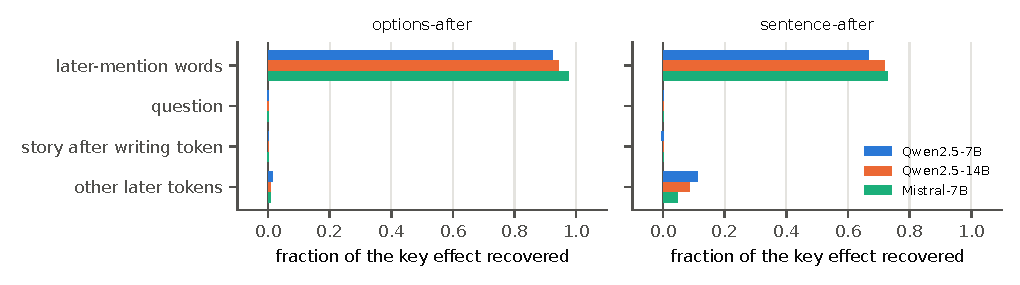
\includegraphics[width=0.85\textwidth]{figures/fig_localisation.pdf}
\caption{\textbf{Which later tokens read the writing token's key} (discovery sample; preregistration D, D3). Fraction of the full key effect recovered when only one group of later tokens sees the source key, at Qwen2.5-7B, Qwen2.5-14B and Mistral-7B, under \fmtOpt{} and \fmtPost{}; $n = 60$ stories; values with intervals in \cref{tab:localisation}.}
\label{fig:localisation}
\end{figure}

\paragraph{Attention probe.} An early exploratory probe at Qwen2.5-1.5B ($n = 25$ cores, no CIs, a different prompt) found that the option word naming the source location attends to the writing token as in the source run when the writing token's key is swapped. Part (a) of preregistration G supersedes it (\cref{app:g-attention}).

\paragraph{Preregistration G.} Preregistration G (GPU stage 5) asked what the duplicate-token account predicts and where it stops. Parts (a)--(d) use the 150 seed-0 story cores of stages 1 and 3b (the row splice and the form probe the first 60 of them), and part (e) 200 fresh IOI cores. Every contrast is paired by core, with 95\% percentile intervals from 10{,}000 core-bootstrap resamples and ratios of means recomputed within each resample. \Cref{tab:prereg-g} gives every verdict; here we define the measures, give the per-cell values and report the observations that the entry did not predict, without reinterpreting them. A shared gate required the stage-5 factorial to reproduce the stage-3b $\mathrm{ID}_K$ of \fmtPost{}, \fmtNone{} and \fmtListA{} in the four models of parts (c) and (d); every value agrees at the printed precision. Triples are Qwen2.5-7B / Qwen2.5-14B / Mistral-7B unless stated.

\subsubsection{(a) Re-mention attention at every scale}\label{app:g-attention}

Under \fmtPost{} the neutral sentence mentions the written word B again. With eager attention, we take for each head the attention from that mention to the writing token, minus the mean attention to the writing token from the candidates not mentioned before it. The three heads with the largest mean excess on the odd-indexed cores form $H^*$. On the even-indexed cores, $E$ is the mean excess at $H^*$, and $F$ is the gain in the attention from the mention of S to the writing token under the key clamp $\mathcal{C}_K(\mathrm{S})$, so $F/E = 1$ means that the attention follows the clamped key one for one. $G$ is the same excess for the answer position's attention to the mention of B (hop~2), at its own three heads, and $Q$ is $G$ at a small model divided by the smaller $G$ of the two anchors, Qwen2.5-7B and 14B. \Cref{tab:attention} gives every cell.

\begin{table}[!ht]
\centering
\small
\caption{\textbf{Re-mention attention} (preregistration G, part (a)). $E$: excess attention of the later mention of B to the writing token at the three selected heads; $F/E$: the share of it that follows the key clamp; $G$: excess attention of the answer position to the mention of B (hop~2) at its own three heads; $\mathrm{ID}_K$ and the non-specific key effect $d_K$ (nats) from the same eager run, scored in the casing the model emits. Heads selected on odd-indexed and evaluated on even-indexed cores of 150; 95\% bootstrap CIs. Under \fmtPost{}: G1 at 7B and 14B, G2 and G3 at 1.5B and 3B, G4 in all four; \fmtOpt{} is the gate and the reference of G3.}
\label{tab:attention}
\begin{tabular}{@{}llccccc@{}}
\toprule
Model & Format & $E$ & $F/E$ & $G$ (hop 2) & $\mathrm{ID}_K$ (nats) & $d_K$ (nats) \\
\midrule
Qwen2.5-1.5B & \fmtPost{} & \begin{tabular}[t]{@{}c@{}}0.789\\[-1pt]{\scriptsize[0.778, 0.802]}\end{tabular} & 1.03 & \begin{tabular}[t]{@{}c@{}}0.086\\[-1pt]{\scriptsize[0.075, 0.098]}\end{tabular} & \begin{tabular}[t]{@{}c@{}}$-$0.53\\[-1pt]{\scriptsize[$-$0.64, $-$0.41]}\end{tabular} & $+$0.31 \\
 & \fmtOpt{} & \begin{tabular}[t]{@{}c@{}}0.750\\[-1pt]{\scriptsize[0.734, 0.767]}\end{tabular} & 1.04 & \begin{tabular}[t]{@{}c@{}}0.453\\[-1pt]{\scriptsize[0.423, 0.484]}\end{tabular} & \begin{tabular}[t]{@{}c@{}}$+$2.63\\[-1pt]{\scriptsize[2.41, 2.86]}\end{tabular} & $+$5.96 \\
\midrule
Qwen2.5-3B & \fmtPost{} & \begin{tabular}[t]{@{}c@{}}0.879\\[-1pt]{\scriptsize[0.866, 0.892]}\end{tabular} & 0.99 & \begin{tabular}[t]{@{}c@{}}0.113\\[-1pt]{\scriptsize[0.095, 0.132]}\end{tabular} & \begin{tabular}[t]{@{}c@{}}$+$0.04\\[-1pt]{\scriptsize[$-$0.35, 0.44]}\end{tabular} & $+$3.03 \\
 & \fmtOpt{} & \begin{tabular}[t]{@{}c@{}}0.832\\[-1pt]{\scriptsize[0.821, 0.844]}\end{tabular} & 1.03 & \begin{tabular}[t]{@{}c@{}}0.395\\[-1pt]{\scriptsize[0.355, 0.435]}\end{tabular} & \begin{tabular}[t]{@{}c@{}}$+$10.37\\[-1pt]{\scriptsize[9.62, 11.13]}\end{tabular} & $+$20.57 \\
\midrule
Qwen2.5-7B & \fmtPost{} & \begin{tabular}[t]{@{}c@{}}0.869\\[-1pt]{\scriptsize[0.852, 0.885]}\end{tabular} & 1.00 & \begin{tabular}[t]{@{}c@{}}0.255\\[-1pt]{\scriptsize[0.222, 0.288]}\end{tabular} & \begin{tabular}[t]{@{}c@{}}$+$4.73\\[-1pt]{\scriptsize[4.39, 5.07]}\end{tabular} & $+$9.21 \\
 & \fmtOpt{} & \begin{tabular}[t]{@{}c@{}}0.887\\[-1pt]{\scriptsize[0.874, 0.900]}\end{tabular} & 1.00 & \begin{tabular}[t]{@{}c@{}}0.770\\[-1pt]{\scriptsize[0.739, 0.798]}\end{tabular} & \begin{tabular}[t]{@{}c@{}}$+$19.39\\[-1pt]{\scriptsize[19.00, 19.78]}\end{tabular} & $+$36.90 \\
\midrule
Qwen2.5-14B & \fmtPost{} & \begin{tabular}[t]{@{}c@{}}0.915\\[-1pt]{\scriptsize[0.908, 0.921]}\end{tabular} & 0.98 & \begin{tabular}[t]{@{}c@{}}0.329\\[-1pt]{\scriptsize[0.304, 0.353]}\end{tabular} & \begin{tabular}[t]{@{}c@{}}$+$13.48\\[-1pt]{\scriptsize[12.76, 14.20]}\end{tabular} & $+$24.09 \\
 & \fmtOpt{} & \begin{tabular}[t]{@{}c@{}}0.866\\[-1pt]{\scriptsize[0.856, 0.876]}\end{tabular} & 0.99 & \begin{tabular}[t]{@{}c@{}}0.865\\[-1pt]{\scriptsize[0.859, 0.872]}\end{tabular} & \begin{tabular}[t]{@{}c@{}}$+$38.95\\[-1pt]{\scriptsize[37.88, 39.97]}\end{tabular} & $+$74.79 \\
\bottomrule
\end{tabular}

\end{table}

At 1.5B and 3B the re-mention attends to the writing token about as strongly as at 7B and 14B, and the attention follows the clamped key, while $\mathrm{ID}_K$ under \fmtPost{} stays within the preregistered $\pm 1$-nat margin (G2, $H_{\mathrm{diss}}$; G3). By the entry's criterion the heads are not embedding-level, and the same heads serve both formats at 1.5B and 7B (overlap of the two $H^*$, as a Jaccard index, \GaJaccardQwenOnefive{} and \GaJaccardQwenSeven{}; \GaJaccardQwenThree{} at 3B). Hop-2 attention is weaker at the small models ($Q$ = \GfourbQQwenOnefive{} and \GfourbQQwenThree{}; G4), but at 3B it reaches the presence bar that G4a sets for the anchors without any key read, so it does not alone account for the scale difference. $G$ measures attention; it does not intervene on hop~2.

\emph{Unpredicted observations.} (i)~At 3B the key clamp has a non-specific effect without identity ($d_K$ = \GaDKCapPostQwenThree{} nats against $\mathrm{ID}_K$ = \GaIDKCapPostQwenThree{}). (ii)~Under \fmtPost{} only \GaCompetentPostQwenOnefive{} and \GaCompetentPostQwenThree{} of the cores at the small models are answered correctly in both clean runs, and almost every wrong answer is the initial location; on the competent cores the 3B value is slightly positive, as in the stage-1 competent-only analysis (\cref{app:additional}; recomputed, not preregistered). (iii)~Under the key clamp, the answer's hop-2 attention does not follow the clamped key at 1.5B (change towards the mention of S \GaDansSPostQwenOnefive{}, towards B \GaDansBPostQwenOnefive{}), partly follows it at 3B (\GaDansSPostQwenThree{} and $\GaDansBPostQwenThree$) and follows it at 7B and 14B (\GaDansSPostQwenSeven{} and $\GaDansBPostQwenSeven$; \GaDansSPostQwenFourteen{} and $\GaDansBPostQwenFourteen$). (iv)~Under \fmtPost{} at 7B and 14B, the answer row at the hop-2 heads attends mostly to the writing token itself (\GaAnsToPQwenSeven{} and \GaAnsToPQwenFourteen{}), not to the re-mentions; under \fmtOpt{} its five largest columns are all re-mentioned words. (v)~The two formats' $H^*$ overlap little at 14B (\GaJaccardQwenFourteen{}), but each format's heads still work on the other (cross-format $E$ = \GaEcrossPostQwenFourteen{} and \GaEcrossOptQwenFourteen{}).

\subsubsection{(b) Attention knockout}\label{app:g-knockout}

A knockout sets the attention from a set of rows to a set of columns to zero in every layer and head (\cref{app:impl}). The preregistered masks are M0, none; M1, the six candidate words after the writing token to the writing token; M2, the same rows to the earlier occurrences of the initial-location word, a matched control column; M3, the answer position to the writing token; M4, the union of M1 and M3; and M8, every later row to the writing token, a sanity gate. The exploratory masks are M2b, the candidate rows to the token before the writing token; M5, only the rows of the three clamped candidates B, S and X; M6, the other three candidate rows; M7, every later row that is not a candidate word; Mq, the question rows; and Mpost, the rows between the candidates and the answer position. $r_K$ is $\mathrm{ID}_K$ under the mask divided by $\mathrm{ID}_K$ without it; $q_V = \mathrm{ID}_V/d_{KV}$ is the value identity as a share of the joint clamp's effect; acc$_B$ is the fraction of cores whose answer, restricted to the candidates, is still B. \Cref{tab:knockout} gives every cell.

\begin{table}[!ht]
\centering
\small
\caption{\textbf{Attention knockout} (preregistration G, part (b); masks in the text). $r_K$: $\mathrm{ID}_K$ under the mask relative to no mask; $q_V$: $\mathrm{ID}_V$ as a share of the joint clamp's effect $d_{KV}$; acc$_B$: fraction of cores whose candidate-restricted answer is B. $n = 150$ cores per cell. M1, M2, M3, M4 and M8 enter G5--G8 and Gate b; the other masks, and every mask under \fmtPost{}, are exploratory. Under \fmtNone{} only the masks that do not need candidate rows are defined.}
\label{tab:knockout}
\begin{tabular}{@{}llccccccccc@{}}
\toprule
Format & Mask & \multicolumn{3}{c}{Qwen2.5-7B} & \multicolumn{3}{c}{Qwen2.5-14B} & \multicolumn{3}{c}{Mistral-7B} \\
\cmidrule(lr){3-5}\cmidrule(lr){6-8}\cmidrule(lr){9-11}
 & & $r_K$ & $q_V$ & acc$_B$ & $r_K$ & $q_V$ & acc$_B$ & $r_K$ & $q_V$ & acc$_B$ \\
\midrule
\fmtListA{} & M0 & 1.000 & 0.125 & 1.00 & 1.000 & 0.075 & 1.00 & 1.000 & 0.105 & 1.00 \\
 & M1 & 0.001 & 0.390 & 0.37 & $-$0.026 & 0.440 & 1.00 & $-$0.007 & 0.448 & 0.86 \\
 & M2 & 1.094 & 0.104 & 1.00 & 0.997 & 0.065 & 1.00 & 0.990 & 0.113 & 1.00 \\
 & M2b & 1.001 & 0.125 & 1.00 & 1.000 & 0.075 & 1.00 & 1.000 & 0.107 & 1.00 \\
 & M3 & 1.043 & 0.022 & 1.00 & 1.027 & 0.017 & 1.00 & 1.010 & 0.053 & 1.00 \\
 & M4 & 0.001 & 0.512 & 0.00 & 0.001 & 0.470 & 0.66 & $-$0.001 & 0.457 & 0.39 \\
 & M5 & $-$0.008 & 0.418 & 0.73 & $-$0.025 & 0.446 & 1.00 & $-$0.007 & 0.457 & 0.89 \\
 & M6 & 0.961 & 0.117 & 1.00 & 1.003 & 0.071 & 1.00 & 1.003 & 0.106 & 1.00 \\
 & M7 & 0.947 & 0.003 & 0.97 & 1.022 & 0.004 & 1.00 & 0.948 & 0.020 & 0.97 \\
 & M8 & 0.000 & -- & 0.00 & 0.000 & -- & 0.13 & 0.000 & -- & 0.17 \\
 & Mq & 0.981 & 0.123 & 1.00 & 1.002 & 0.076 & 1.00 & 0.988 & 0.112 & 1.00 \\
 & Mpost & 1.001 & 0.119 & 1.00 & 1.002 & 0.068 & 1.00 & 0.999 & 0.096 & 1.00 \\
\midrule
\fmtOpt{} & M0 & 1.000 & 0.120 & 1.00 & 1.000 & 0.066 & 1.00 & 1.000 & 0.074 & 1.00 \\
 & M1 & 0.003 & 0.377 & 0.30 & $-$0.028 & 0.427 & 0.99 & $-$0.009 & 0.422 & 0.73 \\
 & M2 & 1.071 & 0.099 & 1.00 & 0.998 & 0.057 & 1.00 & 0.972 & 0.083 & 1.00 \\
 & M2b & 1.000 & 0.120 & 1.00 & 0.999 & 0.066 & 1.00 & 1.001 & 0.077 & 1.00 \\
 & M3 & 1.041 & 0.019 & 1.00 & 1.017 & 0.013 & 1.00 & 1.006 & 0.040 & 1.00 \\
 & M4 & 0.000 & 0.523 & 0.00 & 0.002 & 0.464 & 0.58 & 0.001 & 0.446 & 0.29 \\
 & M5 & $-$0.004 & 0.404 & 0.58 & $-$0.027 & 0.435 & 1.00 & $-$0.008 & 0.429 & 0.77 \\
 & M6 & 0.971 & 0.113 & 1.00 & 1.005 & 0.059 & 1.00 & 1.007 & 0.077 & 1.00 \\
 & M7 & 0.944 & 0.001 & 0.98 & 0.983 & 0.004 & 1.00 & 0.926 & 0.015 & 0.99 \\
 & M8 & 0.000 & -- & 0.00 & 0.000 & -- & 0.10 & 0.000 & -- & 0.19 \\
 & Mq & 0.980 & 0.119 & 1.00 & 0.997 & 0.068 & 1.00 & 0.993 & 0.079 & 1.00 \\
 & Mpost & 1.001 & 0.118 & 1.00 & 0.998 & 0.065 & 1.00 & 1.000 & 0.070 & 1.00 \\
\midrule
\fmtPost{} & M0 & 1.000 & 0.346 & 1.00 & 1.000 & 0.325 & 1.00 & 1.000 & 0.361 & 1.00 \\
 & M1 & $-$0.105 & 0.423 & 1.00 & $-$0.036 & 0.443 & 1.00 & 0.001 & 0.460 & 0.99 \\
 & M2 & 1.027 & 0.346 & 1.00 & 0.922 & 0.333 & 1.00 & 0.963 & 0.368 & 1.00 \\
 & M2b & 1.007 & 0.346 & 1.00 & 0.994 & 0.327 & 1.00 & 0.991 & 0.362 & 1.00 \\
 & M3 & 1.660 & 0.099 & 0.77 & 1.800 & 0.117 & 1.00 & 1.394 & 0.188 & 0.99 \\
 & M4 & 0.007 & 0.496 & 0.07 & 0.014 & 0.480 & 0.91 & 0.002 & 0.446 & 0.29 \\
 & M5 & $-$0.113 & 0.423 & 1.00 & $-$0.035 & 0.443 & 1.00 & $-$0.003 & 0.464 & 1.00 \\
 & M6 & 0.974 & 0.348 & 1.00 & 1.053 & 0.319 & 1.00 & 0.995 & 0.359 & 1.00 \\
 & M7 & 1.184 & $-$0.036 & 0.35 & 1.939 & $-$0.016 & 1.00 & 1.456 & 0.012 & 0.86 \\
 & M8 & 0.000 & -- & 0.00 & 0.000 & -- & 0.14 & 0.000 & -- & 0.05 \\
 & Mq & 0.929 & 0.349 & 0.99 & 1.005 & 0.323 & 1.00 & 1.000 & 0.359 & 1.00 \\
 & Mpost & 1.028 & 0.329 & 0.99 & 1.327 & 0.255 & 1.00 & 1.209 & 0.290 & 1.00 \\
\midrule
\fmtNone{} & M0 & 1.000 & 0.391 & 1.00 & 1.000 & 0.335 & 1.00 & 1.000 & 0.433 & 1.00 \\
 & M3 & 0.023 & 0.566 & 0.00 & 0.041 & 0.459 & 0.20 & 0.117 & 0.445 & 0.15 \\
 & M8 & 0.000 & -- & 0.00 & 0.000 & -- & 0.00 & 0.000 & -- & 0.12 \\
 & Mq & 0.967 & 0.388 & 1.00 & 1.005 & 0.331 & 1.00 & 0.988 & 0.432 & 1.00 \\
 & Mpost & 1.040 & 0.378 & 1.00 & 1.004 & 0.318 & 1.00 & 0.995 & 0.402 & 1.00 \\
\bottomrule
\end{tabular}

\end{table}

Cutting the candidate words' attention to the writing token removes the key read in every format and model, the control column does not, and cutting the answer's own attention leaves the read intact (G5, G6, G8b). The copy returns to its \fmtNone{} share on the identity measure (G7a), but the answer is kept only at Qwen2.5-14B (G7b): the preregistered outcome is a partial takeover. Under \fmtNone{}, M3 leaves \GeightaRatioQwenSeven{} / \GeightaRatioQwenFourteen{} / \GeightaRatioMistralSeven{} of $\mathrm{ID}_V$ (G8a), but it also removes most of the writing token's whole effect and of the models' ability to answer (\cref{tab:knockout}).

\emph{Unpredicted observations.} (i)~At Qwen2.5-7B, the answer that replaces B under M1 is mostly the initial location (exploratory, recomputed, descriptive); G7b's location-mass criterion cannot see these answers, because they are location words too. (ii)~Under \fmtPost{}, cutting only the answer's attention to the writing token (M3) raises the key read ($r_K$ = \GbRKPostMthreeQwenSeven{} / \GbRKPostMthreeQwenFourteen{} / \GbRKPostMthreeMistralSeven{}), and so does M7. (iii)~Cutting only the rows of the three clamped candidates (M5) removes the read as completely as M1 (under \fmtListA{}, $r_K$ = $\GbRKAfterMfiveQwenSeven$ / $\GbRKAfterMfiveQwenFourteen$ / $\GbRKAfterMfiveMistralSeven$), while cutting the other three (M6) leaves it intact (\GbRKAfterMsixQwenSeven{} / \GbRKAfterMsixQwenFourteen{} / \GbRKAfterMsixMistralSeven{}). (iv)~Under \fmtPost{}, M1 raises $q_V$ to \GbQVPostMoneQwenSeven{} / \GbQVPostMoneQwenFourteen{} / \GbQVPostMoneMistralSeven{}. (v)~At Qwen2.5-7B, cutting the control column (M2) slightly strengthens the key read ($r_K$ = \GsixRKQwenSeven{}).

\subsubsection{(c) Membership and dose}\label{app:g-membership}

The arms replace the neutral sentence (family S) or the option list (family L) by one that names a subset of the candidates, in the canonical order and with ``Answer with one word'': S2 and L2 name S and X; S3 and L3 name B, S and X; S3out and L3out name B and two candidates other than S and X; S3half names B, S and one other; S4 and L4 name B, S, X and one other; S4out and L4out name S, X and two others, but not B; and S6 and L6 are \fmtPost{} and \fmtListA{}. $r_k$ is $\mathrm{ID}_K$ in the arm naming $k$ candidates divided by $\mathrm{ID}_K$ in the arm naming all six. The row splice (first 60 cores) lets only the named words' rows see the source key, giving $f_{\mathrm{words}}$, their share of the total splice effect $d$. \Cref{tab:membership} gives every arm.

\begin{table}[!ht]
\centering
\small
\caption{\textbf{Membership and dose} (preregistration G, part (c)). Top: $\mathrm{ID}_K$ and $\mathrm{ID}_V$ (nats) per arm, seed-0 cores, $n = 150$. Bottom: row splice ($n = 60$), the share of the total key-swap effect $d$ read by the named words' rows ($f_{\mathrm{words}}$) and by the rows after the question. Qwen2.5-7B, Qwen2.5-14B and Mistral-7B enter G9--G12; OLMo-2-7B and the arms S3half, S4, S4out, L4, L4out, S6, L6 (as splice arms) and S3out, L3out (as splice arms) are exploratory.}
\label{tab:membership}
\begin{tabular}{@{}lcccccccc@{}}
\toprule
Arm & \multicolumn{2}{c}{Qwen2.5-7B} & \multicolumn{2}{c}{Qwen2.5-14B} & \multicolumn{2}{c}{Mistral-7B} & \multicolumn{2}{c}{OLMo-2-7B} \\
\cmidrule(lr){2-3}\cmidrule(lr){4-5}\cmidrule(lr){6-7}\cmidrule(lr){8-9}
 & $\mathrm{ID}_K$ & $\mathrm{ID}_V$ & $\mathrm{ID}_K$ & $\mathrm{ID}_V$ & $\mathrm{ID}_K$ & $\mathrm{ID}_V$ & $\mathrm{ID}_K$ & $\mathrm{ID}_V$ \\
\midrule
\fmtNone{} & $+$1.04 & $+$16.60 & $+$1.05 & $+$19.12 & $+$0.55 & $+$13.65 & $+$0.38 & $+$10.97 \\
S2 & $+$1.52 & $+$13.97 & $+$6.99 & $+$23.51 & $+$3.66 & $+$13.22 & $+$0.86 & $+$8.55 \\
S3 & $+$3.49 & $+$11.94 & $+$9.52 & $+$19.67 & $+$5.25 & $+$11.83 & $+$1.51 & $+$8.75 \\
S3half & $+$2.11 & $+$12.13 & $+$5.41 & $+$16.16 & $+$2.66 & $+$11.79 & $+$0.67 & $+$8.37 \\
S3out & $+$0.73 & $+$12.61 & $+$0.75 & $+$13.40 & $+$0.34 & $+$12.18 & $+$0.29 & $+$8.84 \\
S4 & $+$4.59 & $+$12.26 & $+$10.88 & $+$18.88 & $+$6.15 & $+$11.87 & $+$1.64 & $+$8.69 \\
S4out & $+$4.18 & $+$14.08 & $+$10.82 & $+$24.36 & $+$6.17 & $+$13.58 & $+$1.59 & $+$8.96 \\
S6 & $+$5.52 & $+$11.91 & $+$12.08 & $+$18.46 & $+$7.87 & $+$11.46 & $+$2.01 & $+$8.63 \\
\midrule
L2 & $+$19.76 & $+$18.63 & $+$35.19 & $+$29.48 & $+$15.27 & $+$16.24 & $+$5.87 & $+$10.03 \\
L3 & $+$21.70 & $+$4.06 & $+$35.83 & $+$2.97 & $+$15.66 & $+$3.29 & $+$7.89 & $+$5.14 \\
L3out & $+$0.69 & $+$5.49 & $+$0.92 & $+$3.49 & $+$0.31 & $+$2.47 & $+$0.37 & $+$4.30 \\
L4 & $+$21.50 & $+$4.71 & $+$35.87 & $+$4.19 & $+$15.38 & $+$3.62 & $+$8.35 & $+$5.33 \\
L4out & $+$20.29 & $+$14.90 & $+$35.45 & $+$30.76 & $+$15.45 & $+$13.68 & $+$8.00 & $+$9.07 \\
L6 & $+$20.60 & $+$5.93 & $+$35.81 & $+$5.69 & $+$15.55 & $+$3.44 & $+$8.65 & $+$5.93 \\
\midrule
\multicolumn{9}{@{}l}{\emph{Reader rows (splice, $n = 60$): $f_{\mathrm{words}}$ / share read by the rows after the question}} \\
S2 & \multicolumn{2}{c}{0.40 / 0.46} & \multicolumn{2}{c}{0.38 / 0.49} & \multicolumn{2}{c}{0.39 / 0.38} & \multicolumn{2}{c}{0.26 / 0.62} \\
S3 & \multicolumn{2}{c}{0.68 / 0.13} & \multicolumn{2}{c}{0.72 / 0.11} & \multicolumn{2}{c}{0.72 / 0.10} & \multicolumn{2}{c}{0.90 / $-$0.01} \\
S6 & \multicolumn{2}{c}{0.67 / 0.11} & \multicolumn{2}{c}{0.72 / 0.09} & \multicolumn{2}{c}{0.73 / 0.05} & \multicolumn{2}{c}{0.76 / 0.06} \\
S3out & \multicolumn{2}{c}{0.04 / 0.90} & \multicolumn{2}{c}{0.11 / 0.74} & \multicolumn{2}{c}{0.11 / 0.68} & \multicolumn{2}{c}{$-$0.16 / 1.40} \\
L2 & \multicolumn{2}{c}{0.91 / 0.14} & \multicolumn{2}{c}{0.94 / 0.17} & \multicolumn{2}{c}{0.92 / 0.08} & \multicolumn{2}{c}{0.72 / 0.13} \\
L3 & \multicolumn{2}{c}{0.94 / 0.01} & \multicolumn{2}{c}{0.95 / 0.00} & \multicolumn{2}{c}{0.95 / 0.01} & \multicolumn{2}{c}{0.91 / $-$0.01} \\
L6 & \multicolumn{2}{c}{0.91 / 0.01} & \multicolumn{2}{c}{0.93 / 0.01} & \multicolumn{2}{c}{0.95 / 0.01} & \multicolumn{2}{c}{0.88 / 0.00} \\
L3out & \multicolumn{2}{c}{0.58 / 0.13} & \multicolumn{2}{c}{0.39 / 0.09} & \multicolumn{2}{c}{0.41 / 0.18} & \multicolumn{2}{c}{0.58 / 0.31} \\
\bottomrule
\end{tabular}

\end{table}

The key read needs the swapped candidates themselves: naming B with two others gives none (G9, met in both families and replicated at seed~1). In lists two named candidates give the full read; in sentences the read grows with the number named, and at Qwen2.5-7B $r_2$ = \GtenSRtwoQwenSeven{} (\GtenSRtwoSeedoneQwenSeven{} at seed~1) is not above proportional (G10, met for lists, not for sentences). Removing S and X from a list does not bring the copy back ($R_V$ = \GelevenRVQwenSeven{} / \GelevenRVQwenFourteen{} / $\GelevenRVMistralSeven$; G11, not met). In a sentence naming only S and X (S2), the named words carry \GtwelveStwoQwenSeven{} / \GtwelveStwoQwenFourteen{} / \GtwelveStwoMistralSeven{} of the splice effect and the rows after the question \GtwelveRestStwoQwenSeven{} / \GtwelveRestStwoQwenFourteen{} / \GtwelveRestStwoMistralSeven{} (G12, not met, 9/12). G12 splits the total key-swap effect $d$, not $\mathrm{ID}_K$, and in S2 most of $d$ is not identity-specific: $\mathrm{ID}_K/d_K$ is \GcShareStwoQwenSeven{} / \GcShareStwoQwenFourteen{} / \GcShareStwoMistralSeven{} in S2 against \GcShareSthreeQwenSeven{} / \GcShareSthreeQwenFourteen{} / \GcShareSthreeMistralSeven{} in S3 (arithmetic on printed values). The main text's narrowing to ``lists and sentences naming at least three candidates'' rests on this.

\emph{Unpredicted observations.} (i)~Naming B with two other candidates pushes $\mathrm{ID}_K$ below \fmtNone{}, although the written word is re-mentioned (S3out$-$\fmtNone{} $\GnineSOutNoneQwenSeven$, L3out$-$\fmtNone{} $\GnineLOutNoneQwenSeven$ at Qwen2.5-7B; \cref{tab:prereg-g}). (ii)~In sentences every added candidate raises $\mathrm{ID}_K$: at Qwen2.5-7B the paired steps are S3$-$S2 = \GtenSStepThreeTwoQwenSeven{} (adds B), S4$-$S3 = \GtenSStepFourThreeQwenSeven{} (adds one non-matching candidate) and S6$-$S4 = \GtenSStepSixFourQwenSeven{} (adds two), each with a CI excluding zero; a pure duplicate-token account does not predict the last two. Naming one of the two swapped candidates (S3half) gives about half of S3 (\GcHalfQwenSeven{} at Qwen2.5-7B). (iii)~In lists that do not name the written word B, the key read is at full strength while the value identity stays near or above \fmtNone{}: $\mathrm{ID}_V$(L4out) is \GcIDVLfouroutQwenSeven{} / \GcIDVLfouroutQwenFourteen{} / \GcIDVLfouroutMistralSeven{} against \GcIDVNoneQwenSeven{} / \GcIDVNoneQwenFourteen{} / \GcIDVNoneMistralSeven{} under \fmtNone{} and \GcIDVLthreeQwenSeven{} / \GcIDVLthreeQwenFourteen{} / \GcIDVLthreeMistralSeven{} in L3. This suggests, post hoc, that the copy is suppressed when the written word itself is re-mentioned; it is a hypothesis for a future test, not a claim. (iv)~Under \fmtNone{} and every sentence arm, the clean answer puts almost no probability on the six lowercase candidates at the three primary models, so the sentence-family contrasts are scored on tokens the model is not about to emit, as in stage 3b; in lists the candidates carry most of it.

\subsubsection{(d) Non-identical re-mentions}\label{app:g-forms}

Each variant replaces the re-mentions of the \fmtPost{} sentence: THE adds ``the''; MODIF uses a modified noun phrase (``wooden shelf''); TITLE and UPPER change the case; PLURAL uses the plural; SYN a synonym; FRMIX and DEMIX put the French or German word in the English frame; FR and DE translate the whole sentence (exploratory); and three structure-matched floor sentences name other words. With the floor and the exact repeat (\fmtPost{}) scored on the English candidates, $r_K(v) = [\mathrm{ID}_K(v) - \mathrm{ID}_K(\text{floor})]/[\mathrm{ID}_K(\text{\fmtPost{}}) - \mathrm{ID}_K(\text{floor})]$; $r_K^{\mathrm{any}}$ also scores the answer in the variant's own form; $\rho_s$ is the ratio of the identity key shares; and $a_v$ is the variant's attention to the writing token, summed over its tokens, relative to the exact repeat's ($n = 60$). Gates required clean accuracy of at least 0.95 in the variant, its floor and its anchor, and that at least five of the six words map correctly in a six-way prompt (the passing words are the population of the cell). A prediction is met if at least three evaluable models meet it. \Cref{tab:variants} gives every cell.

\begin{table}[!ht]
\centering
\caption{\textbf{Non-identical re-mentions} (preregistration G, part (d)). $r_K$: key identity relative to an exact repeat, above a structure-matched floor, on the English candidates; $r_K^{\mathrm{any}}$: the same with the answer also scored in the variant's own form; $a_v$: attention of the re-mention to the writing token relative to the exact repeat, summed over the re-mention's tokens ($n = 60$). $n = 150$ cores per cell before the per-word competence gate; DEMIX and DE cover fewer cores. THE, MODIF, TITLE, UPPER, PLURAL, SYN, FRMIX and DEMIX enter G13--G16; FR, DE and the list variant are exploratory.}
\label{tab:variants}
\resizebox{\textwidth}{!}{\begin{tabular}{@{}lcccccccccccc@{}}
\toprule
Variant & \multicolumn{3}{c}{Qwen2.5-7B} & \multicolumn{3}{c}{Qwen2.5-14B} & \multicolumn{3}{c}{Mistral-7B} & \multicolumn{3}{c}{OLMo-2-7B} \\
\cmidrule(lr){2-4}\cmidrule(lr){5-7}\cmidrule(lr){8-10}\cmidrule(lr){11-13}
 & $r_K$ & $r_K^{\mathrm{any}}$ & $a_v$ & $r_K$ & $r_K^{\mathrm{any}}$ & $a_v$ & $r_K$ & $r_K^{\mathrm{any}}$ & $a_v$ & $r_K$ & $r_K^{\mathrm{any}}$ & $a_v$ \\
\midrule
THE & 1.09 & 1.09 & 1.09 & 0.99 & 0.99 & 1.02 & 1.06 & 1.06 & 1.11 & 0.96 & 0.96 & 1.02 \\
MODIF & 0.32 & 0.32 & 1.22 & 0.64 & 0.64 & 1.24 & 0.64 & 0.64 & 1.08 & 0.55 & 0.55 & 0.94 \\
TITLE & 0.94 & 1.19 & 0.92 & 1.09 & 1.37 & 0.97 & 1.07 & 1.53 & 1.79 & 0.87 & 0.89 & 0.90 \\
UPPER & 1.08 & 1.51 & 1.74 & 1.14 & 1.57 & 1.93 & 1.01 & 1.26 & 2.58 & 0.83 & 0.90 & 1.84 \\
PLURAL & 0.33 & 0.33 & 0.87 & 0.37 & 0.37 & 0.88 & 0.49 & 0.50 & 1.40 & 0.11 & 0.11 & 0.89 \\
SYN & $-$0.03 & 0.09 & 0.41 & 0.00 & 0.09 & 0.41 & 0.06 & 0.26 & 0.53 & $-$0.13 & $-$0.13 & 0.21 \\
FRMIX & 0.15 & 0.95 & 0.86 & 0.10 & 1.06 & 0.90 & 0.07 & 0.56 & 0.55 & 0.09 & 0.44 & 0.39 \\
DEMIX & $-$0.01 & 0.69 & 0.66 & 0.02 & 1.32 & 0.65 & 0.02 & 0.31 & 0.33 & 0.00 & $-$0.13 & 0.09 \\
FR & 0.18 & 0.55 & 1.16 & 0.18 & 0.47 & 1.21 & 0.14 & 0.28 & 0.83 & 0.16 & 0.41 & 0.58 \\
DE & 0.00 & 0.59 & 0.92 & 0.06 & 1.06 & 1.01 & 0.05 & 0.55 & 0.58 & $-$0.05 & 0.43 & 0.30 \\
list SYN & 0.05 & 0.33 & -- & 0.05 & 0.23 & -- & 0.07 & 0.47 & -- & 0.00 & 0.05 & -- \\
\bottomrule
\end{tabular}
}
\end{table}

On our English-scored measure the read is bound to the word form (G15): synonyms and mixed-language words carry at most \GfifteenRKMax{} of an exact repeat's key identity. It is largely insensitive to case (TITLE and UPPER read \GfourteenCaseMin{}--\GfourteenCaseMax{}; G14 not met for them), sensitive to number (PLURAL \GfourteenPluralMin{}--\GfourteenPluralMax{}), and a modified noun phrase reads only partly (MODIF \GthirteenModifMin{}--\GthirteenModifMax{}; G13 not met for it, THE met). No preregistered token-or-concept outcome holds for any variant (G16, not met): the profile is graded and model-dependent. Per model, and exploratory: at the two Qwen models FRMIX shows the concept pattern on both measures ($r_K^{\mathrm{any}}$ = \GdRKanyFrmixQwenSeven{} and \GdRKanyFrmixQwenFourteen{}; $a_v$ = \GdAvFrmixQwenSeven{} and \GdAvFrmixQwenFourteen{}), and scored in its own form it reads fully ($r_K$ = \GdRKformFrmixQwenSeven{} and \GdRKformFrmixQwenFourteen{}); DEMIX is concept-like on $r_K^{\mathrm{any}}$ but graded on $a_v$ there; at Mistral-7B and OLMo-2-7B the read is graded or token-level. Where the read is lost, the value identity rises (G17, met), but by no more than after the floor sentence that names other words (exploratory: the floor sentence raises $\mathrm{ID}_V$ over \fmtPost{} by \GdOtherCompQwenSeven{}, \GdOtherCompMistralSeven{} and \GdOtherCompOlmoSeven{} nats at Qwen2.5-7B, Mistral-7B and OLMo-2-7B, recomputed, against \GseventeenFrmixQwenSeven{}, \GseventeenFrmixMistralSeven{} and \GseventeenFrmixOlmoSeven{} for FRMIX).

\emph{Unpredicted observations.} (i)~A capitalised or upper-case re-mention reads nearly as fully as the exact repeat, although its token ids differ; the CI lies below 1 in three of the eight cells. (ii)~MODIF attends to the writing token about as much as the exact repeat ($a_v$ = \GdAvModifQwenSeven{}, \GdAvModifQwenFourteen{}, \GdAvModifMistralSeven{} and \GdAvModifOlmoSeven{} in the four models) but reads the key only partly: attention without the read. Values of $a_v$ above 1 come from summing attention over multi-token spans; with the last token only, the FRMIX attention leg falls below the concept bar (exploratory, recomputed in the log). (iii)~The raw rise of $\log p(\mathrm{S})$ under the key clamp does not separate the variants, so only the identity contrasts are reported.

\subsection{Reader heads and the second hop}\label{app:heads}\label{sec:heads}\label{sec:role}\label{app:stage6}

Preregistration H (GPU stage 6) has two parts: the heads that read the writing token's key and the route from them to the answer, at two 7B models (this subsection), and the key-only and value-only exchange applied to the binding intervention of \citet{prakash2025lookbacks} at Qwen2.5-14B (\cref{app:prakash}). \Cref{tab:prereg-h} gives every gate and verdict, and \cref{app:prereg-ai} the disclosures.

\paragraph{Summary (discovery sample).} Preregistration H looked inside the option rows at Qwen2.5-7B and Mistral-7B under \fmtOpt{} (\cref{tab:heads}); H1--H5 were met in both. When only the top 5\% of heads by $a_3$ (\HkstarQwenSeven{} and \HkstarMistralSeven{}) see the source key, they recover $R(k^*) = \HoneRQwenSeven{}$ and \HoneRMistralSeven{} of the option rows' read (H1), and blinding them removes \HtwoKOQwenSeven{} and \HtwoKOMistralSeven{} (H2); random sets of equal size recover \HtwoRrandQwenSeven{} and \HtwoRrandMistralSeven{} and remove \HtwoKOrandQwenSeven{} and \HtwoKOrandMistralSeven{} (three-draw means; \cref{fig:readers}b). Ranking by single-head effect does not find the set, nor does leave-one-out at Qwen2.5-7B, and no layer alone recovers more than \HlayerMaxOptQwenSeven{} (exploratory; below): the read is joint across layers.

Mean-ablating them at the option rows cuts $\mathrm{ID}_K$ to $\rho_K = \HthreeRhoQwenSeven{}$ and \HthreeRhoMistralSeven{} of its value (control sets $\geq \HthreeRhoRandTwoQwenSeven{}$), raises $\mathrm{ID}_V$ by \HthreeDVQwenSeven{} and \HthreeDVMistralSeven{} nats, and leaves the base answer in \HthreeBaseQwenSeven{} and \HthreeBaseMistralSeven{} of stories (H3). The lookup thus suppresses a copy route that stays available. Cutting the candidate words' edges instead (G5) also restores the value identity in 3/3 models but keeps the answer only at Qwen2.5-14B (G7, not met: a preregistered partial takeover); we do not reconcile the two. We do not claim the lookup replaces the copy: its preregistered tests failed (G11; on IOI, G20).

\paragraph{The second hop.} The answer need not attend to the writing token (forbidding it leaves $r_K$ at \GeightbRKMistralSeven{}--\GeightbRKQwenSeven{}; G8b, met at 7--14B); it reads the option words. With the source key clamped, giving only the answer row the option rows' base keys and values removes $r_{\mathrm{ans}} = \HfiveAnsQwenSeven{}$ and \HfiveAnsMistralSeven{} of the key-clamp effect, against \HfiveOtherQwenSeven{} and \HfiveOtherMistralSeven{} for all other later rows (H5, met; \cref{fig:readers}c). Unscored (H5), the answer reads them by key: $r_{\mathrm{ans}}(K) = \HfiveAnsKQwenSeven{}$ and \HfiveAnsKMistralSeven{}, against $r_{\mathrm{ans}}(V) = \HfiveAnsVQwenSeven{}$ and \HfiveAnsVMistralSeven{}. The \fmtPost{} line is not evaluable (below). Without a later mention, the same cut leaves \GeightaRatioQwenSeven{}--\GeightaRatioMistralSeven{} of $\mathrm{ID}_V$ (G8a, met).

\paragraph{What the duplicate-token account explains.} The first hop, a re-mention attending to the writing token, is the pattern of duplicate-token heads \citep{wang2022ioi}. Under \fmtPost{}, the re-mentioned word attends to the writing token far more than the other candidates do, and this attention follows the clamped key one for one, at 7B and 14B ($E$, the excess at the top three heads, = \GoneEQwenSeven{}, \GoneEQwenFourteen{}; $F/E$, its share following the clamp, = \GoneFEQwenSeven{}, \GoneFEQwenFourteen{}; G1) and equally at 1.5B and 3B ($E$ = \GtwoEQwenOnefive{}, \GtwoEQwenThree{}; $F/E$ = \GtwoFEQwenOnefive{}, \GtwoFEQwenThree{}; G2, G3), whose \fmtPost{} key identity was about zero on the lower-case score (within the preregistered $\pm 1$-nat margin). All three were met. Whether the flag that this match writes at 1.5B carries the size of the sentence read was tested in the final round (\cref{app:scale}): the flag is written in sentences as in lists at every scale, the preregistered mediation test came out mixed, and at 1.5B the injected flag is read by key. The core of the causally selected readers is of this kind (H4, met): over the top \HfourKCQwenSeven{} and \HfourKCMistralSeven{} heads by $a_3$, which carry 80\% of the read, the median duplicate-token score $D$ (on random repeated sequences) is \HfourDQwenSeven{} and \HfourDMistralSeven{} (whole-model medians \HfourDwholeQwenSeven{} and \HfourDwholeMistralSeven{}; exploratory, recomputed), the median induction score \citep{olsson2022context} \HfourIQwenSeven{} and \HfourIMistralSeven{}. Only this core is canonical: over the full 5\% set the median $D$ is \HfourDkstarQwenSeven{} and \HfourDkstarMistralSeven{} (exploratory, recomputed).

We therefore claim no new head type. What the discovery sample added is that the answer then reads the re-mentioned words, mainly by key (H5, secondary); the final round tested what these heads write (\cref{app:flag}). The channels carry which value was written, not its belief role (E2, met; \cref{tab:role}).

\begin{figure}[!ht]
  \centering
  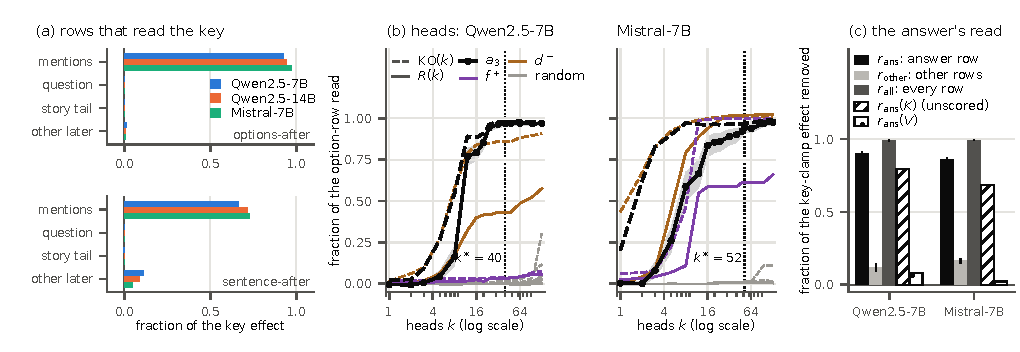
\includegraphics[width=\textwidth]{figures/fig_readers.pdf}
  \caption{\textbf{The later mentions read the writing token's key through a small set of heads, and the answer reads the later mentions} (discovery sample). (a)~Row-restricted splice ($n = 60$; D3): the fraction of the full key effect recovered when only one group of later tokens sees the source key (top \fmtOpt{}, bottom \fmtPost{}). (b)~\fmtOpt{}, 60 held-out stories: $R(k)$ (solid) and $\mathrm{KO}(k)$ (dashed) for heads ranked by $a_3$ (band: 95\% CI), by single-head effect $f^+$ and leave-one-out effect $d^-$, and three random sets (grey); dotted: $k^*$ (H1, H2). (c)~Key-clamp effect removed when only the answer row, all other later rows or all rows get the option rows' base keys and values (H5; hatched, open: keys or values only, not scored). Values in \cref{tab:localisation,tab:heads}.}
  \label{fig:readers}
\end{figure}

\paragraph{Design.} Qwen2.5-7B (\HnHeadsQwenSeven{} heads) and Mistral-7B (\HnHeadsMistralSeven{} heads), BF16 with eager attention; \fmtOpt{} confirmatory, \fmtPost{} reported. Heads are ranked on 60 ranking stories by $a_3$, the attention change of the option rows of S and B towards $p$ under the key clamp ($a_3 = \tfrac12[(A^{K_{\mathrm{S}}} - A^{\mathrm{B}})_{\text{row S} \to p} + (A^{\mathrm{B}} - A^{K_{\mathrm{S}}})_{\text{row B} \to p}]$), and every curve is evaluated on 60 other stories. $R(k)$ is the fraction of the option rows' key effect $d_G$ recovered when only the top $k$ heads see the source key in the option rows (HeadSplice; \cref{app:impl}), and $\mathrm{KO}(k)$ the fraction lost when only they are blinded; $k^* = \lceil 0.05 \times \text{heads} \rceil$ = \HkstarQwenSeven{} and \HkstarMistralSeven{}, and $k_{80}$ is the smallest $k$ on the grid with $R(k) \geq 0.8$. The other rankings are the single-head effect $f^+$ (each head alone sees the source key) and the leave-one-out effect $d^-$ (each head alone is blinded); the controls are three random sets (the first $k^*$ heads of fixed random permutations) and the $k^*$ heads most active at the option rows outside the top $2k^*$ by $a_3$. The duplicate-token score $D$ and the induction score $I$ come from 100 random repeated-token sequences, and the in-task score $T_{\mathrm{dup}}$ is the attention from each option row to the earlier occurrences of the same word other than $p$. The causal set $C$ is the top $\min(k_{80}, k^*)$ heads by $a_3$. \Cref{tab:heads} gives H1--H5, \cref{fig:heads-app} the curves and \cref{tab:ablation} every ablation condition.

\begin{table}[!ht]
\centering
\small
\caption{\textbf{Reader heads and the second hop} (preregistration H, part (a); \fmtOpt{}, 60 held-out stories, BF16). $R(k^*)$, $\mathrm{KO}(k^*)$: fraction of the option rows' key effect recovered when only the top $k^*$ heads by $a_3$ see the source key, or lost when only they are blinded. $\rho_K$: $\mathrm{ID}_K$ under mean-ablation of these heads at the option rows, relative to no ablation. $C$: the top heads by $a_3$ that carry 80\% of the read. $r_{\mathrm{ans}}$: fraction of the key-clamp effect removed when only the answer row gets the option rows' base keys and values; $r_{\mathrm{other}}$, $r_{\mathrm{all}}$: the same for every other later row and for all rows. 95\% bootstrap CIs over stories. The last row is H5's secondary contrast, reported, not scored.}
\label{tab:heads}
\begin{tabular}{@{}llcc@{}}
\toprule
 & Quantity (\fmtOpt{}) & Qwen2.5-7B & Mistral-7B \\
\midrule
 & heads $k^*$ (of all heads) & 40 (784) & 52 (1024) \\
\midrule
H1 & $R(k^*)$, top-$k^*$ by $a_3$ see $K_S$ & \begin{tabular}[t]{@{}c@{}}0.967\\[-1pt]{\scriptsize[0.952, 0.982]}\end{tabular} & \begin{tabular}[t]{@{}c@{}}0.942\\[-1pt]{\scriptsize[0.919, 0.961]}\end{tabular} \\
 & $k_{80}$ by $a_3$ / by $f^+$ / by $d^-$ & 20 / none / none & 16 / none / 12 \\
\midrule
H2 & $\mathrm{KO}(k^*)$, top-$k^*$ blinded & \begin{tabular}[t]{@{}c@{}}0.977\\[-1pt]{\scriptsize[0.966, 0.987]}\end{tabular} & \begin{tabular}[t]{@{}c@{}}0.971\\[-1pt]{\scriptsize[0.954, 0.984]}\end{tabular} \\
 & random sets: $R$ / $\mathrm{KO}$ (mean of 3) & 0.004 / 0.011 & 0.007 / 0.010 \\
\midrule
H3 & $\rho_K$ under mean-ablation of the top-$k^*$ & \begin{tabular}[t]{@{}c@{}}0.238\\[-1pt]{\scriptsize[0.205, 0.270]}\end{tabular} & \begin{tabular}[t]{@{}c@{}}0.059\\[-1pt]{\scriptsize[0.040, 0.079]}\end{tabular} \\
 & $\rho_K$, control sets (min--max) & 0.953--1.018 & 1.002--1.009 \\
 & rise of $\mathrm{ID}_V$ (nats) & \begin{tabular}[t]{@{}c@{}}$+$6.907\\[-1pt]{\scriptsize[6.264, 7.561]}\end{tabular} & \begin{tabular}[t]{@{}c@{}}$+$10.861\\[-1pt]{\scriptsize[9.995, 11.677]}\end{tabular} \\
 & answer kept (base argmax) & 0.87 & 1.00 \\
\midrule
H4 & $|C|$ (top heads by $a_3$ carrying 80\,\%) & 20 & 16 \\
 & median duplicate score $D$ over $C$ & \begin{tabular}[t]{@{}c@{}}0.370\\[-1pt]{\scriptsize[0.361, 0.378]}\end{tabular} & \begin{tabular}[t]{@{}c@{}}0.232\\[-1pt]{\scriptsize[0.227, 0.238]}\end{tabular} \\
 & median induction score $I$ over $C$ & 0.011 & 0.022 \\
 & median in-task $T_{\mathrm{dup}}$ over $C$ & 0.459 & 0.433 \\
 & top-10 by $a_3$ $\cap$ top-10 by $D$ & 6 & 5 \\
\midrule
H5 & $r_{\mathrm{ans}}$: only the answer row restored & \begin{tabular}[t]{@{}c@{}}0.899\\[-1pt]{\scriptsize[0.886, 0.913]}\end{tabular} & \begin{tabular}[t]{@{}c@{}}0.859\\[-1pt]{\scriptsize[0.845, 0.872]}\end{tabular} \\
 & $r_{\mathrm{other}}$ / $r_{\mathrm{all}}$ & 0.118 / 0.992 & 0.165 / 0.992 \\
 & $r_{\mathrm{ans}}(K)$ / $r_{\mathrm{ans}}(V)$ (secondary, not scored) & 0.797 / 0.080 & 0.683 / 0.023 \\
\bottomrule
\end{tabular}

\end{table}

\begin{figure}[!ht]
\centering
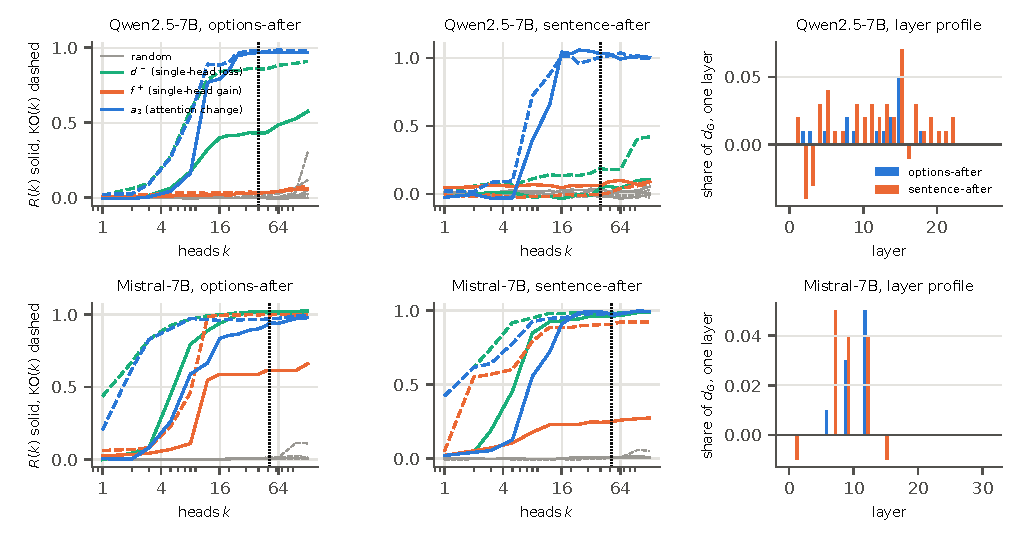
\includegraphics[width=\textwidth]{figures/fig_heads_app.pdf}
\caption{\textbf{Head curves and layer profiles} (preregistration H, part (a); exploratory except $R(k^*)$ and $\mathrm{KO}(k^*)$ of the $a_3$ ranking under \fmtOpt{}). Left and middle: $R(k)$ (solid) and $\mathrm{KO}(k)$ (dashed) against the number of heads $k$ for the rankings by $a_3$, single-head effect $f^+$ and leave-one-out effect $d^-$, and for three random sets (grey), under \fmtOpt{} and \fmtPost{}; dotted: $k^*$. Right: the share of the option rows' key effect recovered when all heads of one layer see the source key. 60 held-out stories per model and format.}
\label{fig:heads-app}
\end{figure}

\paragraph{Sufficiency and necessity (H1, H2).} The top 5\% of heads recover almost all of the option rows' read and blinding them removes almost all of it, while random sets of equal size do neither; no single random draw exceeds $R$ = \HtwoRrandMaxQwenSeven{} / \HtwoRrandMaxMistralSeven{} or $\mathrm{KO}$ = \HtwoKOrandMaxQwenSeven{} / \HtwoKOrandMaxMistralSeven{} (exploratory, recomputed). The ranking is stable: the split-half Spearman correlation of $a_3$ between ranking and evaluation stories is \HsplitOptQwenSeven{} / \HsplitOptMistralSeven{} under \fmtOpt{} and \HsplitPostQwenSeven{} / \HsplitPostMistralSeven{} under \fmtPost{}.

\paragraph{The read is a joint property of many heads (exploratory).} Ranking by single-head effect does not find the set, and ranking by leave-one-out effect finds it at one of the two models: at Qwen2.5-7B, $f^+$ reaches only $R(128)$ = \HcurveRFplusHundredandtwentyeightOptQwenSeven{} and $d^-$ \HcurveRDminusHundredandtwentyeightOptQwenSeven{}; at Mistral-7B $f^+$ reaches \HcurveRFplusHundredandtwentyeightOptMistralSeven{}, while $d^-$ reaches $k_{80}$ = \HoneKeightyDminusMistralSeven{}, fewer heads than $a_3$ needs (\HoneKeightyMistralSeven{}). The $a_3$ curve rises steeply (Qwen2.5-7B: $R(8)$ = \HcurveRAthreeEightOptQwenSeven{}, $R(12)$ = \HcurveRAthreeTwelveOptQwenSeven{}), and at Mistral-7B blinding the top three heads removes \HcurveKOAthreeThreeOptMistralSeven{} of the read while the same three alone recover \HcurveRAthreeThreeOptMistralSeven{}. Letting all heads of a single layer read the source key recovers at most \HlayerMaxOptQwenSeven{} (layer \HlayerArgOptQwenSeven{}) and \HlayerMaxOptMistralSeven{} (layer \HlayerArgOptMistralSeven{}) of $d_G$, and the single-layer shares sum to only \HlayerSumOptQwenSeven{} and \HlayerSumOptMistralSeven{} (exploratory, recomputed); the heads of $C$ span \HlayerSpanQwenSeven{} and \HlayerSpanMistralSeven{} layers (exploratory, recomputed). No single head or layer is necessary or sufficient; the top \HfourKCQwenSeven{} and \HfourKCMistralSeven{} heads by $a_3$, over many layers, are, jointly.

\begin{table}[!ht]
\centering
\caption{\textbf{Every ablation condition} (preregistration H, part (a); 60 held-out stories). $\rho_K$: $\mathrm{ID}_K$ under ablation at the six option rows, relative to none; $\Delta\mathrm{ID}_V$: rise of the value identity (nats); kept: fraction of stories whose candidate-restricted clean answer is still B. ``mean'': mean-ablation with the head's position-matched mean over the ranking stories; ``zero'': zero-ablation. H3 uses the top-$k^*$ mean row, the three random sets and the most-active set under \fmtOpt{}; every other cell is exploratory.}
\label{tab:ablation}
\resizebox{\textwidth}{!}{\begin{tabular}{@{}lcccccccccccc@{}}
\toprule
Condition & \multicolumn{3}{c}{Qwen2.5-7B, \fmtOpt{}} & \multicolumn{3}{c}{Qwen2.5-7B, \fmtPost{}} & \multicolumn{3}{c}{Mistral-7B, \fmtOpt{}} & \multicolumn{3}{c}{Mistral-7B, \fmtPost{}} \\
\cmidrule(lr){2-4}\cmidrule(lr){5-7}\cmidrule(lr){8-10}\cmidrule(lr){11-13}
 & $\rho_K$ & $\Delta\mathrm{ID}_V$ & kept & $\rho_K$ & $\Delta\mathrm{ID}_V$ & kept & $\rho_K$ & $\Delta\mathrm{ID}_V$ & kept & $\rho_K$ & $\Delta\mathrm{ID}_V$ & kept \\
\midrule
none & 1.000 & $+$0.000 & 0.97 & 1.000 & $+$0.000 & 1.00 & 1.000 & $+$0.000 & 1.00 & 1.000 & $+$0.000 & 1.00 \\
top-$k^*$ (mean) & 0.238 & $+$6.907 & 0.87 & $-$0.080 & $+$2.295 & 1.00 & 0.059 & $+$10.861 & 1.00 & 0.012 & $+$2.640 & 1.00 \\
top-10 (mean) & 0.859 & $+$1.978 & 0.98 & 0.616 & $+$1.436 & 1.00 & 0.139 & $+$12.326 & 1.00 & 0.233 & $+$2.302 & 0.98 \\
top-20 (mean) & 0.654 & $+$4.285 & 0.95 & 0.126 & $+$2.282 & 1.00 & 0.104 & $+$12.728 & 1.00 & 0.056 & $+$2.648 & 1.00 \\
top-$k^*$ (zero) & 0.081 & $+$11.315 & 1.00 & $-$0.060 & $+$2.756 & 1.00 & 0.057 & $+$9.030 & 0.95 & 0.006 & $+$2.609 & 1.00 \\
random set 1 & 1.002 & $+$0.091 & 0.97 & 0.969 & $+$0.081 & 1.00 & 1.002 & $-$0.096 & 1.00 & 1.003 & $+$0.048 & 1.00 \\
random set 2 & 0.978 & $+$0.851 & 1.00 & 0.655 & $+$0.820 & 1.00 & 1.009 & $-$0.292 & 1.00 & 1.289 & $-$1.563 & 1.00 \\
random set 3 & 0.953 & $+$0.241 & 0.98 & 0.975 & $+$0.114 & 1.00 & 1.006 & $-$0.326 & 1.00 & 1.100 & $-$0.336 & 1.00 \\
most active at $G$ & 1.018 & $-$0.177 & 0.97 & 0.934 & $+$0.012 & 1.00 & 1.009 & $+$0.049 & 1.00 & 0.949 & $+$0.521 & 1.00 \\
next $k^*$ by $a_3$ & 1.019 & $-$0.062 & 1.00 & 1.140 & $-$0.028 & 1.00 & 0.996 & $+$0.173 & 1.00 & 0.823 & $+$0.682 & 1.00 \\
\bottomrule
\end{tabular}
}
\end{table}

\paragraph{Ablation (H3).} Mean-ablating the top-$k^*$ heads at the option rows removes most of the key identity, raises the value identity and keeps the answer; the random and most-active sets of equal size leave $\rho_K$ near 1 (\cref{tab:ablation}). Zero-ablation (exploratory) goes the same way ($\rho_K$ = \HablTopkzeroRhoOptQwenSeven{} and \HablTopkzeroRhoOptMistralSeven{}). Without ablation the answer is B in \HablNoneBaseOptQwenSeven{} of Qwen2.5-7B stories, against \HthreeBaseQwenSeven{} under ablation. The rise of the value identity is partial at Qwen2.5-7B ($\mathrm{ID}_V$ under ablation \HablIDVafterQwenSeven{} nats against \idVNoneQwenSeven{} under \fmtNone{} in stage 1), and at Mistral-7B it reaches about the \fmtNone{} level (\HablIDVafterMistralSeven{} against \idVNoneMistralSeven{}); both comparisons are across stages and stories (arithmetic on printed values). The stage-5 edge knockout keeps the answer only at Qwen2.5-14B (G7b); the two interventions differ (mean-ablation at six rows leaves $\rho_K$ = \HthreeRhoQwenSeven{} at Qwen2.5-7B, the knockout leaves $r_K \approx 0$), and we do not reconcile them.

\paragraph{Duplicate-token heads (H4) and the size of $C$.} Over $C$ the median previous-token score is \HcPrevOptQwenSeven{} / \HcPrevOptMistralSeven{} (largest \HfourPrevMaxQwenSeven{} / \HfourPrevMaxMistralSeven{}, exploratory, recomputed), and the in-task score of control words that are not candidates is \HcTctrlOptQwenSeven{} / \HcTctrlOptMistralSeven{}, against $T_{\mathrm{dup}}$ = \HfourTQwenSeven{} / \HfourTMistralSeven{}. $T_{\mathrm{dup}}$ is measured in the task the heads were selected on, so we treat it as supporting rather than independent evidence; $D$ and $I$, on random sequences, are the test. H4 depends on the size of the head set (exploratory, recomputed): only \HfourNDgeQwenSeven{} of the \HfourKCQwenSeven{} heads of $C$ at Qwen2.5-7B and \HfourNDgeMistralSeven{} of the \HfourKCMistralSeven{} at Mistral-7B have $D \geq 0.2$, against \HfourNDgeWholeQwenSeven{} and \HfourNDgeWholeMistralSeven{} in the whole model, whose median $D$ is \HfourDwholeQwenSeven{} / \HfourDwholeMistralSeven{}. Over the full top-$k^*$ set (exploratory) the median $D$ is \HfourDkstarQwenSeven{} / \HfourDkstarMistralSeven{}; at Mistral-7B it is \HfourDtopTwentyMistralSeven{} over the top 20 and \HfourDtopTwelveMistralSeven{} over the top 12. At Qwen2.5-7B (exploratory), $R(16)$ = \HoneRsixteenQwenSeven{}, just under 0.8, so $C$ has 20 heads; over the top 16 the median $D$ would also be \HfourDtopSixteenQwenSeven{}. Over all heads, $a_3$ correlates weakly with $D$ (Spearman \HfourRhoDQwenSeven{} / \HfourRhoDMistralSeven{}) and with $T_{\mathrm{dup}}$ (\HfourRhoTQwenSeven{} / \HfourRhoTMistralSeven{}). We therefore say that the core of the readers, the top heads by $a_3$ that carry 80\% of the read, is canonical duplicate-token heads, not that every reader is one.

\paragraph{The second hop in detail (H5).} The routes add up: $r_{\mathrm{ans}} + r_{\mathrm{other}}$ = \HhopSumOptQwenSeven{} / \HhopSumOptMistralSeven{} against $r_{\mathrm{all}}$ = \HfiveAllQwenSeven{} / \HfiveAllMistralSeven{}. Restricted to single option rows, the source word's row gives $r_{\mathrm{ans}}$ = \HhoprowRowsAnsKVOptQwenSeven{} / \HhoprowRowsAnsKVOptMistralSeven{}, the base word's row \HhoprowRowbAnsKVOptQwenSeven{} / \HhoprowRowbAnsKVOptMistralSeven{} and the separators \HhoprowSepAnsKVOptQwenSeven{} / \HhoprowSepAnsKVOptMistralSeven{} (exploratory). As H5's secondary contrast, reported and not scored, the answer reads the option rows mainly through their keys ($r_{\mathrm{ans}}(K) - r_{\mathrm{ans}}(V)$ = \HfiveKminusVQwenSeven{} / \HfiveKminusVMistralSeven{}, CIs excluding zero), and the strong version $r_{\mathrm{ans}}(KV) \geq 0.7$ holds in both models.

\paragraph{\fmtPost{} (reported, not scored).} Gate a2 failed at Qwen2.5-7B under \fmtPost{} (\cref{app:prereg}), so H6 and H5's \fmtPost{} line are not evaluable; the values below are exploratory. The option-row ceiling covers less of the full effect than under \fmtOpt{} ($d_G/d_{\mathrm{full}}$ = \HathreeRatioPostQwenSeven{} / \HathreeRatioPostMistralSeven{}, exploratory, recomputed). At Qwen2.5-7B, $R(k)$ and $\mathrm{KO}(k)$ exceed 1 (\cref{fig:heads-app}), and mean-ablation of the top $k^*$ drives $\rho_K$ to $\HablTopkRhoPostQwenSeven$; one random set changes $\rho_K$ substantially in each model (\cref{tab:ablation}). The answer row's read gives $r_{\mathrm{ans}}$ = \HfivesAnsQwenSeven{} / \HfivesAnsMistralSeven{}, mainly through keys ($r_{\mathrm{ans}}(K)$ = \HhopAnsKPostQwenSeven{} / \HhopAnsKPostMistralSeven{}, $r_{\mathrm{ans}}(V)$ = $\HhopAnsVPostQwenSeven$ / \HhopAnsVPostMistralSeven{}). The top-20 heads by $a_3$ of the two formats share \HsixOverlapQwenSeven{} and \HsixOverlapMistralSeven{} heads (H6's threshold is 10; met at Mistral-7B, not evaluable at Qwen2.5-7B), the top 10 share \HcrossToptenQwenSeven{} and \HcrossToptenMistralSeven{}, and the full $a_3$ grids correlate at Spearman \HcrossRhoQwenSeven{} / \HcrossRhoMistralSeven{} (exploratory, recomputed). In this free-form format the candidates carry little of the clean answer's probability, so H3's candidate-mass criterion fails in every condition, as expected.

\paragraph{Ablation against knockout (not reconciled).} Mean-ablating the reader heads at the six option rows (H3) keeps the base answer, while cutting the candidate words' attention to the writing token (G5) keeps it only at Qwen2.5-14B (G7b): the two interventions differ, and the discovery sample does not reconcile them. The passage tests of the final round that would have bridged them were not evaluable (\cref{app:natural}).

\subsection{What the reader heads write: the flag}\label{app:flag}

\begin{figure}[!ht]
  \centering
  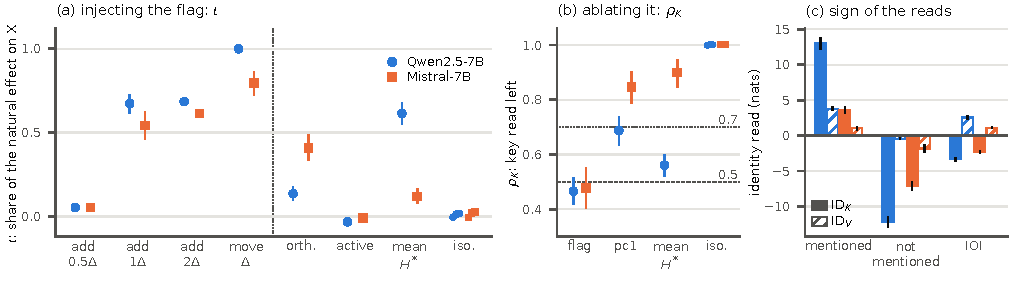
\includegraphics[width=\textwidth]{figures/fig_flag.pdf}
  \caption{\textbf{What the reader heads write.} Qwen2.5-7B and Mistral-7B; flags fit on 60 discovery-sample stories, tested on 100 others (60 in (b)); 95\,\% story-bootstrap intervals, the fit fixed. (a)~$\iota$: effect on an absent option X relative to the natural key clamp's, for the flag ($\Delta$) added 0.5, 1 or 2 times at X's row (exploratory) or moved there from B's row, and for controls: orth., the story's own write without its flag component; active, the flag of the most active heads; mean $H^*$, the reader heads' mean output; iso., isotropic directions. (b)~$\rho_K$: key read left when one direction per layer is removed at the option rows (pc1: the heads' top principal direction); dashed, dotted: the bounds for the flag and the controls. (c)~$\mathrm{ID}_K$, $\mathrm{ID}_V$ when asked which option is or is not mentioned, and in IOI.}
  \label{fig:flag}
\end{figure}

\paragraph{Definitions.} Let $H^*$ be the reader heads of the discovery sample (the top 5\,\% by $a_3$ under \fmtOpt{}, frozen: 40 heads at Qwen2.5-7B, 52 at Mistral-7B). Under the natural key clamp $K_{\mathrm{S}}$, the heads' summed write at layer $l$ into the rows of S and B changes; the \emph{flag} $\Delta_l$ is the mean over the 60 ranking stories of half the sum of the change at S's row and minus the change at B's row, projected through each head's output matrix, one vector per layer that holds an $H^*$ head. Leave-one-word-out flags $\Delta^{-w}$ are fit on the stories in which $w$ is neither B nor S. An \emph{injection} adds a vector to the attention output at chosen rows, in the clean base run, with no key clamp; ``move'' adds the flag at an option's row and subtracts it at B's row. With $\ell_w$ the six-way log-probability of candidate $w$ and $N_X$ the natural key clamp's effect on X, $\iota$ = the injection's mean effect on $\ell_X$ divided by $N_X$; $\pi_X$ = the share of stories whose answer becomes X; $\mathrm{ID}_{\mathrm{inj}}$ = the identity contrast of moving the flag to S against X; $\rho_K(u)$ = $\mathrm{ID}_K$ with the direction $u$ removed at the six option rows, relative to none; $r_{\mathrm{ans}}^{\mathrm{inj}}(C)$ = the share of the injection's effect removed when only the answer row reads the option rows' clean channel $C$. Scale (\cref{app:scale}): $\omega$, how far the flag written in a sentence matches the list's along the list flag; $c_{\mathrm{fl}}$, the cosine of the sentence and list flags; $\rho$ and $\rho_{\mathrm{nat}}$, the injected and natural sentence-to-list ratios. Binding: $\Psi_{\mathrm{bind}}$, the double difference of initial-state flags under two binding questions. The runs are BF16 with sdpa attention, except the passes that fix the head sets (eager), and every ratio is taken within one run; the intervals are over stories, conditional on the fitted flag and the frozen heads. \Cref{tab:flag} gives every line. The intervals of this subsection resample stories with the flag's fit held fixed: they exclude the uncertainty of the fit itself, which matters because several criteria were decided near their thresholds: J-D2's differences (0.385 and 0.384 against 0.4), Qwen2.5-7B's $\rho_K$ of the top principal direction (\JdThreeRhoPconeQwenSeven{} against 0.7) and Mistral-7B's $\rho_K$ of the flag (\JdThreeRhoFlagMistralSeven{} against 0.5). These decisions lie within an uncertainty the intervals do not show, and J-D1's intervals are narrower than a refit inside each resample would give; that refit was not run. % verbatim: "0.385 / 0.384 against 0.4", outcome J part D % verbatim: 40 and 52 heads, entry J part D

\begin{table}[!ht]
\centering
\caption{\textbf{The flag: every line of the mechanism tests.} Top: Qwen2.5-7B and Mistral-7B, flags fit on 60 discovery-sample stories and tested on 100 new ones (the ablations of J-D3 on the first 60 of them); bottom: the scale lines at Qwen2.5-1.5B, 3B and 7B (\cref{app:scale}). 95\,\% story-bootstrap intervals. $Q_{\mathrm{IN}}$, $Q_{\mathrm{OUT}}$: \fmtOpt{} asked which option is (is not) mentioned; IOI in-sentence: the four names listed right after the indirect object's mention (\cref{app:sign}). n.e.: not evaluable (gate in brackets). $^\dagger$Recomputed: at 3B the line is not evaluable (too few competent cores), and the post hoc rows are not printed by the scorer.}
\label{tab:flag}
\scalebox{0.8}{\begin{minipage}{1.2\textwidth}\centering\footnotesize
\setlength{\tabcolsep}{4pt}
\begin{tabular}{@{}lllll@{}}
\toprule
Line & Statistic & Qwen2.5-7B & Mistral-7B & Verdict \\
\midrule
J-D1 & $\mathrm{ID}^{\mathrm{LOO}}_{\mathrm{inj}}/\mathrm{ID}_K$ & 0.997 [0.980, 1.014] & 0.803 [0.746, 0.856] & \textbf{met} \\
 & $\pi_X$ & 0.96 & 0.67 &  \\
J-D2 & $\iota$(move $\Delta$) & 0.999 [0.992, 1.006] & 0.794 [0.719, 0.864] & \textbf{not met} \\
 & $\iota$(own write $\perp$ flag) & 0.135 [0.096, 0.179] & 0.409 [0.332, 0.488] &  \\
 & $\iota$(mean $H^*$ output) & 0.614 [0.549, 0.679] & 0.120 [0.078, 0.166] &  \\
 & $\iota$(active-set flag) & $-$0.032 [$-$0.037, $-$0.027] & $-$0.010 [$-$0.015, $-$0.006] &  \\
J-D3 & $\rho_K$(flag) & 0.466 [0.416, 0.516] & 0.478 [0.403, 0.553] & \textbf{not met} \\
 & $\rho_K$(pc1) & 0.687 [0.633, 0.738] & 0.846 [0.786, 0.902] &  \\
 & $\rho_K$(mean $H^*$ output) & 0.561 [0.520, 0.600] & 0.899 [0.846, 0.946] &  \\
J-D4 & $r^{\mathrm{inj}}_{\mathrm{ans}}(KV)$ & 0.869 [0.855, 0.884] & 0.762 [0.737, 0.786] & \textbf{met} \\
 & $r^{\mathrm{inj}}_{\mathrm{ans}}(K)$ & 0.689 [0.642, 0.735] & 0.601 [0.540, 0.659] &  \\
 & $r^{\mathrm{inj}}_{\mathrm{ans}}(V)$ & 0.047 [0.030, 0.067] & 0.068 [0.035, 0.104] &  \\
 & $r^{\mathrm{inj}}_{\mathrm{ans}}(K) - r^{\mathrm{inj}}_{\mathrm{ans}}(V)$ & 0.642 [0.589, 0.692] & 0.533 [0.478, 0.588] &  \\
J-D-ADDR & weighted $\cos(\Delta^K, \Delta^{KV})$ & 0.993 & 0.962 & \textbf{met} \\
 & $\mathrm{ID}_{\mathrm{inj}}(KV)/\mathrm{ID}_{\mathrm{inj}}(K)$ & 1.005 [1.003, 1.008] & 0.981 [0.949, 1.013] &  \\
J-D-KN & Pearson (per story) & 0.894 [0.868, 0.917] & 0.147 [0.041, 0.252] & \textbf{not met} \\
 & B-loss ratio $\beta$ & 5.167 [3.878, 7.704] & 9.095 [2.862, 58.110] &  \\
 & mean$(\Delta\ell_S - \Delta\ell_X)$ (nats) & $-$0.073 [$-$0.763, 0.612] & 0.290 [$-$0.457, 1.024] &  \\
J-D5 & $\Psi_{\mathrm{bind}}$ pooled (nats) & $-$0.578 [$-$0.863, $-$0.308] & 0.269 [0.096, 0.456] & \textbf{not met} \\
 & object-first & 0.376 [0.156, 0.619] & 0.459 [0.120, 0.848] &  \\
 & distractor-first & $-$1.299 [$-$1.678, $-$0.955] & 0.126 [$-$0.034, 0.283] &  \\
 & stratum difference & 1.675 [1.272, 2.115] & 0.333 [$-$0.049, 0.751] &  \\
J-D7 & $\mathrm{ID}_K(Q_{\mathrm{OUT}})$ (nats) & $-$12.138 [$-$12.905, $-$11.413] & $-$7.083 [$-$7.726, $-$6.463] & \textbf{met} \\
 & $\mathrm{ID}_K(Q_{\mathrm{IN}})$ (nats) & 13.005 [12.206, 13.777] & 3.575 [3.085, 4.059] &  \\
 & paired difference (nats) & 25.143 [24.121, 26.159] & 10.658 [9.897, 11.413] &  \\
J-D-SIGN-Q & $\mathrm{ID}_V(Q_{\mathrm{OUT}})$ (nats) & $-$0.431 [$-$0.616, $-$0.254] & $-$1.806 [$-$2.442, $-$1.192] & \textbf{met} \\
J-D-SIGN-IOI & $\mathrm{ID}_K$, IOI in-sentence (nats) & $-$3.350 [$-$3.655, $-$3.042] & $-$2.352 [$-$2.542, $-$2.162] & \textbf{met} \\
 & $\mathrm{ID}_V$, IOI in-sentence (nats) & 2.550 [2.244, 2.889] & 1.096 [0.945, 1.247] &  \\
J-D8-Q & $R(H^*)$, $Q_{\mathrm{IN}}$ & 1.027 [1.016, 1.038] & 1.058 [1.032, 1.087] & \textbf{met} \\
 & $\mathrm{KO}(H^*)$, $Q_{\mathrm{IN}}$ & 0.974 [0.968, 0.980] & 0.931 [0.892, 0.964] &  \\
 & $R(H^*)$, $Q_{\mathrm{OUT}}$ & 0.986 [0.971, 1.002] & 1.050 [1.011, 1.093] &  \\
 & $\mathrm{KO}(H^*)$, $Q_{\mathrm{OUT}}$ & 1.021 [1.001, 1.041] & 0.958 [0.918, 0.995] &  \\
J-D8-IOI & $R(H^*)$, IOI in-sentence & 0.922 [0.882, 0.960] & n.e.\ (J-D-G4 INLINE) & \textbf{not evaluable} \\
 & $\mathrm{KO}(H^*)$, IOI in-sentence & 0.998 [0.980, 1.016] & n.e.\ (J-D-G4 INLINE) &  \\
J-D-ROUTE-IOI & $r_{\mathrm{ans}}(KV)$ & 0.897 [0.821, 0.976] & 0.839 [0.769, 0.910] & \textbf{met} \\
 & $r_{\mathrm{ans}}(K)$ & 0.431 [0.318, 0.536] & 0.488 [0.406, 0.567] &  \\
 & $r_{\mathrm{ans}}(V)$ & 0.211 [0.163, 0.267] & 0.263 [0.231, 0.298] &  \\
 & $r_{\mathrm{ans}}(K) - r_{\mathrm{ans}}(V)$ & 0.220 [0.081, 0.343] & 0.225 [0.131, 0.314] &  \\
 & $r_{\mathrm{other}}$ & 0.103 [0.064, 0.146] & 0.190 [0.157, 0.223] &  \\
J-D-HOP2 & carry, top-10 hop-2 heads, $Q_{\mathrm{OUT}}$ & 0.077 [0.062, 0.092] & 0.161 [0.117, 0.208] & \textbf{not met} \\
 & carry, top-10 hop-2 heads, IOI & $-$0.085 [$-$0.141, $-$0.036] & $-$0.029 [$-$0.093, 0.025] &  \\
\bottomrule
\end{tabular}

\medskip

\begin{tabular}{@{}llcccl@{}}
\toprule
Line & Statistic & Qwen2.5-1.5B & Qwen2.5-3B & Qwen2.5-7B & Verdict \\
\midrule
J-D6a & $\omega$ & \begin{tabular}[t]{@{}c@{}}0.967\\[-1pt]{\scriptsize[0.952, 0.982]}\end{tabular} & \begin{tabular}[t]{@{}c@{}}0.954\\[-1pt]{\scriptsize[0.937, 0.971]}\end{tabular} & \begin{tabular}[t]{@{}c@{}}0.822\\[-1pt]{\scriptsize[0.810, 0.834]}\end{tabular} & \textbf{met} \\
 & $c_{\mathrm{fl}}$ & 0.966 & 0.895 & 0.872 &  \\
J-D6 & $\rho$ & \begin{tabular}[t]{@{}c@{}}$-$0.126\\[-1pt]{\scriptsize[$-$0.179, $-$0.077]}\end{tabular} & \begin{tabular}[t]{@{}c@{}}$-$0.025$^\dagger$ (n.e.)\\[-1pt]{\scriptsize [$-$0.104, 0.050]}\end{tabular} & \begin{tabular}[t]{@{}c@{}}0.257\\[-1pt]{\scriptsize[0.222, 0.292]}\end{tabular} & \textbf{not met} \\
 & $\rho_{\mathrm{nat}}$ & \begin{tabular}[t]{@{}c@{}}0.090\\[-1pt]{\scriptsize[0.042, 0.137]}\end{tabular} & \begin{tabular}[t]{@{}c@{}}0.266$^\dagger$ (n.e.)\\[-1pt]{\scriptsize [0.196, 0.341]}\end{tabular} & \begin{tabular}[t]{@{}c@{}}0.468\\[-1pt]{\scriptsize[0.431, 0.505]}\end{tabular} &  \\
 & $\rho - \rho_{\mathrm{nat}}$ & \begin{tabular}[t]{@{}c@{}}$-$0.216\\[-1pt]{\scriptsize[$-$0.273, $-$0.163]}\end{tabular} & \begin{tabular}[t]{@{}c@{}}$-$0.290$^\dagger$ (n.e.)\\[-1pt]{\scriptsize [$-$0.376, $-$0.213]}\end{tabular} & \begin{tabular}[t]{@{}c@{}}$-$0.211\\[-1pt]{\scriptsize[$-$0.245, $-$0.178]}\end{tabular} &  \\
J-D6-ROUTE & $r^{\mathrm{inj}}_{\mathrm{ans}}(V)$ & \begin{tabular}[t]{@{}c@{}}$-$0.140\\[-1pt]{\scriptsize[$-$0.276, $-$0.054]}\end{tabular} & -- & -- & \textbf{not met} \\
 & $r^{\mathrm{inj}}_{\mathrm{ans}}(K)$ & \begin{tabular}[t]{@{}c@{}}1.114\\[-1pt]{\scriptsize[1.006, 1.285]}\end{tabular} & -- & -- &  \\
 & $r^{\mathrm{inj}}_{\mathrm{ans}}(V) - r^{\mathrm{inj}}_{\mathrm{ans}}(K)$ & \begin{tabular}[t]{@{}c@{}}$-$1.254\\[-1pt]{\scriptsize[$-$1.543, $-$1.075]}\end{tabular} & -- & -- &  \\
J-D6, post hoc & natural ratio, $X$-specific contrast$^\dagger$ & \begin{tabular}[t]{@{}c@{}}$-$0.113\\[-1pt]{\scriptsize[$-$0.213, $-$0.030]}\end{tabular} & -- & \begin{tabular}[t]{@{}c@{}}0.271\\[-1pt]{\scriptsize[0.234, 0.308]}\end{tabular} & -- \\
 & $\rho$ minus it$^\dagger$ & \begin{tabular}[t]{@{}c@{}}$-$0.013\\[-1pt]{\scriptsize[$-$0.099, 0.083]}\end{tabular} & -- & \begin{tabular}[t]{@{}c@{}}$-$0.014\\[-1pt]{\scriptsize[$-$0.049, 0.022]}\end{tabular} &  \\
 & natural ratio on $\mathrm{ID}_K$$^\dagger$ & \begin{tabular}[t]{@{}c@{}}$-$0.115\\[-1pt]{\scriptsize[$-$0.182, $-$0.062]}\end{tabular} & -- & \begin{tabular}[t]{@{}c@{}}0.290\\[-1pt]{\scriptsize[0.270, 0.311]}\end{tabular} &  \\
 & $\rho$ minus it$^\dagger$ & \begin{tabular}[t]{@{}c@{}}$-$0.011\\[-1pt]{\scriptsize[$-$0.079, 0.061]}\end{tabular} & -- & \begin{tabular}[t]{@{}c@{}}$-$0.033\\[-1pt]{\scriptsize[$-$0.066, $-$0.002]}\end{tabular} &  \\
D6b & $\Delta^{\mathrm{sentence}}/\Delta^{\mathrm{list}}$ at the list row & \begin{tabular}[t]{@{}c@{}}0.926\\[-1pt]{\scriptsize[0.908, 0.942]}\end{tabular} & \begin{tabular}[t]{@{}c@{}}0.926\\[-1pt]{\scriptsize[0.892, 0.961]}\end{tabular} & \begin{tabular}[t]{@{}c@{}}0.943\\[-1pt]{\scriptsize[0.924, 0.961]}\end{tabular} & reported \\
\bottomrule
\end{tabular}
\end{minipage}}
\end{table}

\paragraph{Sufficiency and identity (J-D1, risky, held; J-D-ADDR, held).} Moved into the row of an option absent from the story (added there and subtracted at B's row, as the natural key clamp moves it), the flag fit without that option's word moves the answer there: $\mathrm{ID}_{\mathrm{inj}}^{\mathrm{LOO}}/\mathrm{ID}_K$ = \JdOneRatioQwenSeven{} [\JdOneRatioQwenSevenLo{}, \JdOneRatioQwenSevenHi{}] and \JdOneRatioMistralSeven{} [\JdOneRatioMistralSevenLo{}, \JdOneRatioMistralSevenHi{}], and the answer changes in $\pi_X$ = \JdOnePiXQwenSeven{} and \JdOnePiXMistralSeven{} of stories. The mean flag names no candidate: fit from the natural source run instead of the key clamp it is the same direction (norm-weighted cosine \JdAddrCosQwenSeven{} and \JdAddrCosMistralSeven{}) with the same effect (ratio \JdAddrRatioQwenSeven{} [\JdAddrRatioQwenSevenLo{}, \JdAddrRatioQwenSevenHi{}] and \JdAddrRatioMistralSeven{} [\JdAddrRatioMistralSevenLo{}, \JdAddrRatioMistralSevenHi{}]). Added alone, without the subtraction at B's row (which keeps its own flag), the flag has less effect: half a flag barely moves the answer, and one and two flags saturate below the full effect, consistent with competition among flagged rows (post hoc reading; adding half, one and two flags at X's row gives $\iota$ = \JdDoseHalfQwenSeven{}, \JdDoseOneQwenSeven{}, \JdDoseTwoQwenSeven{} and \JdDoseHalfMistralSeven{}, \JdDoseOneMistralSeven{}, \JdDoseTwoMistralSeven{}); the full flag gives $\mathrm{ID}_{\mathrm{inj}}/\mathrm{ID}_K$ = \JdFullFlagQwenSeven{} and \JdFullFlagMistralSeven{}; isotropic, head-span, layer-permuted and wrongly placed flags (at the ``Choices'' and ``Question'' rows) give $\lvert\iota\rvert \leq \JdSanityAbsMax{}$ (reported).

\paragraph{Specificity (J-D2, risky, not held).} The line required three structured controls to move the answer at most 0.3 as much as the flag. The active-set flag (the same construction over the heads most active at the option rows) does not move it ($\iota$ = \JdTwoIotaActiveQwenSeven{} and \JdTwoIotaActiveMistralSeven{}), but at Qwen2.5-7B the mean reader output at the option rows, norm-matched, moves it \JdTwoRatioMeanHQwenSeven{} as much as the flag, and at Mistral-7B the story's own write with its flag component removed, norm-matched, \JdTwoRatioOrthMistralSeven{} as much. The checks found (exploratory, recomputed) that the Qwen control overlaps the flag by construction: the clean reader output at the option rows contains the flag written at the mentioned words' rows (norm-weighted cosine 0.636), 54\,\% of the flag's energy lies along the mean-output directions and 29\,\% along the top principal direction, and ablating the mean output reproduces the flag's value-channel signature. The overlap explains much but not all of the failure (a linear energy estimate gives $\rho_K$ about 0.71 and 0.85 for the two Qwen controls), and Mistral's controls overlap the flag too (cosine 0.58) yet pass. The Mistral failure on the orthogonal own write points to a story-specific write (rank-one capture \JdRankOneMistralSeven{}, against \JdRankOneQwenSeven{} at Qwen). % verbatim: outcome J part D

\paragraph{Necessity (J-D3, risky, not held).} Removing the flag direction at the six option rows, one direction per layer, leaves $\rho_K$ = \JdThreeRhoFlagQwenSeven{} [\JdThreeRhoFlagQwenSevenLo{}, \JdThreeRhoFlagQwenSevenHi{}] and \JdThreeRhoFlagMistralSeven{} [\JdThreeRhoFlagMistralSevenLo{}, \JdThreeRhoFlagMistralSevenHi{}] of the key read: about half in both models. The line also required two control directions, the top principal direction of the heads' output and the mean reader output, to leave at least 0.7. At Mistral they do (\JdThreeRhoPconeMistralSeven{} and \JdThreeRhoMeanHMistralSeven{}) and the line holds there, with the flag's point estimate close to its 0.5 floor; at Qwen they remove 31\,\% and 44\,\% (they leave \JdThreeRhoPconeQwenSeven{} and \JdThreeRhoMeanHQwenSeven{}) because they overlap the flag, and the line fails. % verbatim: "31 % and 44 %", outcome J part D
 Isotropic directions leave \JdRhoIsoMin{}--\JdRhoIsoMax{} (reported). The pre-written replacement used in the main text: ``One direction per layer does not carry the key read ($\rho_K$ = \JdThreeRhoFlagQwenSeven{} / \JdThreeRhoFlagMistralSeven{}): other carriers exist; the flag is sufficient but not necessary.'' Whole-head ablation of the reader heads removes far more of the read (discovery sample: $\rho_K$ = \HthreeRhoQwenSeven{} and \HthreeRhoMistralSeven{}; \cref{tab:ablation}), so the heads write more than this direction. % verbatim: J-D3 text, outcome J part D

\paragraph{Read by key (J-D4, held).} Giving only the answer row the option rows' clean keys and values removes $r_{\mathrm{ans}}^{\mathrm{inj}}(KV)$ = \JdFourKVQwenSeven{} and \JdFourKVMistralSeven{} of the injected flag's effect; their clean keys alone \JdFourKQwenSeven{} and \JdFourKMistralSeven{}, their clean values alone \JdFourVQwenSeven{} and \JdFourVMistralSeven{} ($K - V$ = \JdFourKmVQwenSeven{} [\JdFourKmVQwenSevenLo{}, \JdFourKmVQwenSevenHi{}] and \JdFourKmVMistralSeven{} [\JdFourKmVMistralSevenLo{}, \JdFourKmVMistralSevenHi{}]); every other later row carries \JdFourOtherQwenSeven{} and \JdFourOtherMistralSeven{} (reported). The answer reads the injected flag by key, as it reads the natural one (discovery sample, H5).

\paragraph{What the flag is (reported).} Its largest cosine with the unembeddings of the locations is \JdLensMaxQwenSeven{} at Qwen and \JdLensMaxMistralSeven{} at Mistral (both at layer \JdLensLayerQwenSeven{}), against at most \JdLensRandMaxQwenSeven{} and \JdLensRandMaxMistralSeven{} for random token rows: it is not a readable location word. The share of the per-story flag's variance explained by the identity of B is \JdBidShareMin{}--\JdBidShareMax{} across layers, against a null of \JdBidShareNull{}: the mean flag is identity-free, while each story's write also carries its own word.

\paragraph{A key that names no candidate (J-D-KN, risky, not held).} Clamping the writing token's key to a word that is not a candidate (``garage'', ``kitchen'', \ldots) was predicted to act like removing B's flag. Per story, its effects on the six candidates correlate with those of subtracting the flag at B's row at Qwen (Pearson \JdKnPearsonQwenSeven{}) but not at Mistral (\JdKnPearsonMistralSeven{}), and the loss of support for B is far larger than the flag's ($\beta$ = \JdKnBetaQwenSeven{} and \JdKnBetaMistralSeven{} against the preregistered 0.7--1.3); the third criterion held (\JdKnDiffQwenSeven{} and \JdKnDiffMistralSeven{} nats against tolerances of \JdKnTolQwenSeven{} and \JdKnTolMistralSeven{}). The printed sizes are inflated, because at Qwen $p(\mathrm{B}) > 0.99$ in every clean story and at Mistral the denominator is nearly inert; on the six-way logit of B, $\beta$ is 1.93 [1.78, 2.10] and 5.20 [3.38, 10.49] (exploratory, recomputed): a non-candidate key removes about two (Qwen) to five (Mistral) times more support for B than subtracting the mean flag at B's row. % verbatim: outcome J part D

\paragraph{Binding (J-D5, risky, not held).} The flags of the two initial-state sentences were predicted to carry which object they bind, in both sentence orders. Pooled, $\Psi_{\mathrm{bind}}$ = \JdFivePooledQwenSeven{} [\JdFivePooledQwenSevenLo{}, \JdFivePooledQwenSevenHi{}] at Qwen (below zero) and \JdFivePooledMistralSeven{} [\JdFivePooledMistralSevenLo{}, \JdFivePooledMistralSevenHi{}] at Mistral; the two orders differ at Qwen (object first \JdFiveObjQwenSeven{}, distractor first \JdFiveDisQwenSeven{} nats; difference \JdFiveDiffQwenSeven{} [\JdFiveDiffQwenSevenLo{}, \JdFiveDiffQwenSevenHi{}]). The pre-written replacement: ``The initial-state flag does not carry binding in a way separable from order.'' The order effect is a property of the model, not of the fit (the fit set is balanced, 23 against 22 stories), and the two initial-state flags are nearly collinear (weighted cosine 0.97 in both models), so $\Psi_{\mathrm{bind}}$ is a 0.2--1.1-nat contrast on injection effects of 12--19 nats; Mistral's pass is fragile (distractor first \JdFiveDisMistralSeven{} [\JdFiveDisMistralSevenLo{}, \JdFiveDisMistralSevenHi{}]). % verbatim: outcome J part D

\paragraph{Other tasks (exploratory).} The belief flag injected into the paint and schedule tasks gives \JdXtaskPaintQwenSeven{} of the tasks' own flag at Qwen, and \JdXtaskPaintMistralSeven{} and \JdXtaskScheduleMistralSeven{} at Mistral.

\paragraph{Holm sensitivity.} Over the 27 interval components of this part's risky lines with a verdict, Holm's step-down changes no decision and no verdict. % verbatim: outcome J part D

\subsection{The sign of the read, and IOI}\label{app:sign}

\paragraph{The question sets the sign (J-D7, J-D-SIGN-Q, J-D8-Q, held).} Asked which option is \emph{not} mentioned in the story ($Q_{\mathrm{OUT}}$), the key read turns negative: $\mathrm{ID}_K$ = \JdSevenQoutQwenSeven{} [\JdSevenQoutQwenSevenLo{}, \JdSevenQoutQwenSevenHi{}] and \JdSevenQoutMistralSeven{} [\JdSevenQoutMistralSevenLo{}, \JdSevenQoutMistralSevenHi{}] nats, against \JdSevenQinQwenSeven{} and \JdSevenQinMistralSeven{} when asked which option is mentioned ($Q_{\mathrm{IN}}$; paired differences \JdSevenDiffQwenSeven{} and \JdSevenDiffMistralSeven{}). The value read turns negative too ($\mathrm{ID}_V$ = \JdSignQIDVQwenSeven{} [\JdSignQIDVQwenSevenLo{}, \JdSignQIDVQwenSevenHi{}] and \JdSignQIDVMistralSeven{} [\JdSignQIDVMistralSevenLo{}, \JdSignQIDVMistralSevenHi{}]), so the sign follows the task, not a polarity of the readers. The same frozen reader heads carry the read under both questions: when only they see the clamped key they recover $R$ = \JdEightQinRQwenSeven{} and \JdEightQinRMistralSeven{} of it under $Q_{\mathrm{IN}}$ and \JdEightQoutRQwenSeven{} and \JdEightQoutRMistralSeven{} under $Q_{\mathrm{OUT}}$, blinding them removes \JdEightQinKOQwenSeven{}--\JdEightQoutKOQwenSeven{} at Qwen and \JdEightQinKOMistralSeven{}--\JdEightQoutKOMistralSeven{} at Mistral, and random sets of the same size do neither (their $R$ and KO lie between $-0.006$ and $+0.015$). % verbatim: outcome J part D
 Behaviourally, under $Q_{\mathrm{OUT}}$ the key clamp makes the story's own location the answer in \pct{\JdQoutKSQwenSeven} and \pct{\JdQoutKSMistralSeven} of stories, and the list flag injected at X's row moves the answer \JdNineQoutRatioQwenSeven{} and \JdNineQoutRatioMistralSeven{} as much as the natural clamp (reported; under $Q_{\mathrm{IN}}$ \JdNineQinRatioQwenSeven{} and \JdNineQinRatioMistralSeven{}): the readers' write need not change with the question, and the sign is applied after the first hop (exploratory). A negative use of duplicate detection is known \citep{wang2022ioi,mcdougall2023copy}; we do not present the polarity as a discovery.

\paragraph{IOI separates the channels (J-D-SIGN-IOI, held).} In the in-sentence re-mentions of indirect-object identification (the four names listed right after the indirect object's mention), the key read is negative while the value read stays positive: $\mathrm{ID}_K$ = \JdSignIoiIDKQwenSeven{} [\JdSignIoiIDKQwenSevenLo{}, \JdSignIoiIDKQwenSevenHi{}] and \JdSignIoiIDKMistralSeven{} [\JdSignIoiIDKMistralSevenLo{}, \JdSignIoiIDKMistralSevenHi{}] nats, $\mathrm{ID}_V$ = \JdSignIoiIDVQwenSeven{} and \JdSignIoiIDVMistralSeven{} (fresh IOI cores; the discovery sample had shown the same, \cref{app:g-ioi}).

\paragraph{Where the negative read is applied (J-D-ROUTE-IOI, risky, held).} With the key clamp at the indirect object, restoring the listed names' clean keys and values for the answer row alone removes $r(KV)$ = \JdRouteKVQwenSeven{} and \JdRouteKVMistralSeven{} of the read, their keys alone \JdRouteKQwenSeven{} and \JdRouteKMistralSeven{}, their values alone \JdRouteVQwenSeven{} and \JdRouteVMistralSeven{} ($K - V$ = \JdRouteKmVQwenSeven{} [\JdRouteKmVQwenSevenLo{}, \JdRouteKmVQwenSevenHi{}] and \JdRouteKmVMistralSeven{} [\JdRouteKmVMistralSevenLo{}, \JdRouteKmVMistralSevenHi{}]); every other row carries \JdRouteOtherQwenSeven{} and \JdRouteOtherMistralSeven{}. The line tests $K > V$; the key alone carries less than half of the read.

\paragraph{Which heads apply it (J-D-HOP2, risky, not held).} The ten answer-side heads ranked as the flag's top readers in lists were predicted to carry the negative reads too. They carry \JdHopTwoQoutCarryQwenSeven{} and \JdHopTwoQoutCarryMistralSeven{} of the injected flag's effect under $Q_{\mathrm{OUT}}$ and \JdHopTwoInlineCarryQwenSeven{} and \JdHopTwoInlineCarryMistralSeven{} in IOI, while every head together carries \JdHopTwoQoutAllQwenSeven{} and \JdHopTwoQoutAllMistralSeven{} (\JdHopTwoInlineAllQwenSeven{} and \JdHopTwoInlineAllMistralSeven{} in IOI); the scorer's reading is ``different reader''. The reading is confounded: in lists (\fmtOpt{}), the format in which they were ranked, the same ten heads carry only \JdHopOptTopQwenSeven{} and \JdHopOptTopMistralSeven{} of hop 2 (every head \JdHopOptAllQwenSeven{} and \JdHopOptAllMistralSeven{}), so ten heads do not carry hop 2 even there. The pre-written replacement: ``a different (or a distributed) reader applies the negative read''.

\paragraph{The belief readers in IOI (J-D8-IOI, risky, not evaluable).} At Qwen2.5-7B the frozen belief reader heads carry the IOI read ($R$ = \JdEightIoiRQwenSeven{} [\JdEightIoiRQwenSevenLo{}, \JdEightIoiRQwenSevenHi{}], blinding them removes \JdEightIoiKOQwenSeven{}, random sets \JdEightIoiRrandQwenSeven{} and \JdEightIoiKOrandQwenSeven{}). At Mistral-7B the transfer gate (the option rows must carry at least half of the in-sentence key read) missed by 0.021 (\JdGfourRatioInlineMistralSeven{}), so the line, which needs both models, is not evaluable; with the gate passed, Mistral's values (0.938 and 1.030) would meet the criteria and the line would be met. At Qwen the same heads also carry the IOI list read ($R$ = \JdCellAfterRQwenSeven{}, KO = \JdCellAfterKOQwenSeven{}; reported). The line is therefore reported as met at Qwen2.5-7B and not evaluable at Mistral-7B, not as a result about both models. % verbatim numbers 0.021, 0.938, 1.030: outcome J part D, Sensitivities

\paragraph{The IOI factorial of the discovery sample.} The in-sentence IOI arm was first run in preregistration G (part (e), below), whose later-list predictions failed; the final round used the in-sentence arm because it dissociates the channels.

\subsubsection{The IOI factorial of the discovery sample (preregistration G, part (e))}\label{app:g-ioi}

The IOI cores follow the templates of \citet{wang2022ioi}, alternating ABBA and BABA, with four names: the indirect object of the base and source runs and of the third-value run, and the subject. The clamps act at the indirect object's mention. Arms: PLAIN (the sentence); AFTER (a ``Choices:'' list of the four names after the sentence, in the chat wrapper on instruct models); BEFORE (the list before it); QUESTION (``Which name completes the sentence?'', without candidates); and INLINE and INLINE\_BEFORE (the list as a parenthetical right after the indirect object's mention, or before the sentence; preregistered only at GPT-2 small). $f_K = \mathrm{ID}_K/\mathrm{ID}_{KV}$ and $f_V$ likewise. A cell is evaluable only if the clean model passes Gate e: two-way accuracy at least 0.75, four-way at least 0.50, and a positive mean logit difference. GPT-2 small and GPT-2 XL ran in FP32 with exactness asserted, the 7B and 14B models in BF16. \Cref{tab:ioi} gives every cell.

\begin{table}[!ht]
\centering
\caption{\textbf{IOI} (preregistration G, part (e); 200 fresh cores). Gate e: two-way / four-way accuracy of the clean run (failed cells are not evaluable). $\mathrm{ID}_K$ with 95\% bootstrap CI, $\mathrm{ID}_V$ and $\mathrm{ID}_{KV}$ in nats; $f_K$, $f_V$: shares of $\mathrm{ID}_{KV}$, unstable where $\mathrm{ID}_{KV}$ is near zero. GPT-2 small, Qwen2.5-7B-Instruct and Mistral-7B enter G18--G22 (the GPT-2 small parts replicate a disclosed pilot); Qwen2.5-7B base, Qwen2.5-14B-Instruct and GPT-2 XL are exploratory.}
\label{tab:ioi}
\resizebox{\textwidth}{!}{\begin{tabular}{@{}llcccccc@{}}
\toprule
Model & Arm & Gate e (2-way / 4-way) & $\mathrm{ID}_K$ (nats) & $\mathrm{ID}_V$ & $\mathrm{ID}_{KV}$ & $f_K$ & $f_V$ \\
\midrule
GPT-2 & PLAIN & 0.98 / 0.98 & $-$0.15 [$-$0.18, $-$0.11] & $+$14.08 & $+$8.61 & $-$0.02 & $+$1.64 \\
 & AFTER & 0.48 / 0.36 (failed) & $-$1.77 [$-$1.84, $-$1.71] & $+$2.37 & $+$0.93 & $-$1.92 & $+$2.57 \\
 & BEFORE & 0.55 / 0.35 (failed) & $-$0.05 [$-$0.07, $-$0.04] & $+$1.00 & $+$0.89 & $-$0.06 & $+$1.13 \\
 & QUESTION & 0.49 / 0.49 (failed) & $-$0.04 [$-$0.06, $-$0.02] & $+$5.35 & $+$4.37 & $-$0.01 & $+$1.23 \\
 & INLINE & 0.94 / 0.91 & $-$2.35 [$-$2.47, $-$2.23] & $+$6.71 & $+$3.74 & $-$0.63 & $+$1.79 \\
 & INLINE\_BEFORE & 0.91 / 0.82 & $-$0.25 [$-$0.29, $-$0.21] & $+$4.80 & $+$3.27 & $-$0.08 & $+$1.47 \\
\midrule
Qwen2.5-7B & PLAIN & 1.00 / 1.00 & $+$0.20 [0.10, 0.31] & $+$6.72 & $+$10.33 & $+$0.02 & $+$0.65 \\
 & AFTER & 0.98 / 0.89 & $+$7.05 [6.26, 7.81] & $+$5.34 & $+$11.96 & $+$0.59 & $+$0.45 \\
 & BEFORE & 0.97 / 0.82 & $-$2.02 [$-$2.18, $-$1.86] & $+$6.37 & $+$7.67 & $-$0.26 & $+$0.83 \\
 & QUESTION & 1.00 / 1.00 & $+$0.61 [0.43, 0.78] & $+$17.77 & $+$25.90 & $+$0.02 & $+$0.69 \\
 & INLINE & 1.00 / 0.67 & $-$3.26 [$-$3.47, $-$3.05] & $+$2.63 & $+$2.02 & $-$1.61 & $+$1.30 \\
 & INLINE\_BEFORE & 1.00 / 0.62 & $-$0.74 [$-$0.80, $-$0.67] & $+$1.17 & $+$1.43 & $-$0.52 & $+$0.82 \\
\midrule
Mistral-7B & PLAIN & 0.99 / 0.99 & $+$0.02 [$-$0.02, 0.07] & $+$6.06 & $+$7.94 & $+$0.00 & $+$0.76 \\
 & AFTER & 0.59 / 0.42 (failed) & $-$1.98 [$-$2.38, $-$1.58] & $+$3.35 & $+$3.16 & $-$0.63 & $+$1.06 \\
 & BEFORE & 0.81 / 0.27 (failed) & $-$0.96 [$-$1.12, $-$0.80] & $-$2.32 & $-$1.01 & $+$0.95 & $+$2.30 \\
 & QUESTION & 0.96 / 0.96 & $+$0.11 [0.03, 0.18] & $+$11.33 & $+$12.98 & $+$0.01 & $+$0.87 \\
 & INLINE & 1.00 / 0.71 & $-$2.33 [$-$2.46, $-$2.19] & $+$1.27 & $+$1.01 & $-$2.29 & $+$1.25 \\
 & INLINE\_BEFORE & 0.99 / 0.32 (failed) & $-$0.42 [$-$0.48, $-$0.37] & $-$0.26 & $-$0.01 & $+$43.18 & $+$26.44 \\
\midrule
Qwen2.5-7B base (expl.) & PLAIN & 1.00 / 1.00 & $+$0.18 [0.10, 0.26] & $+$5.45 & $+$8.53 & $+$0.02 & $+$0.64 \\
 & AFTER & 0.85 / 0.77 & $-$0.03 [$-$0.15, 0.08] & $+$1.02 & $+$1.72 & $-$0.02 & $+$0.59 \\
 & BEFORE & 0.83 / 0.66 & $-$0.95 [$-$1.01, $-$0.89] & $+$0.76 & $+$0.92 & $-$1.03 & $+$0.82 \\
 & QUESTION & 0.55 / 0.59 (failed) & $+$0.27 [0.19, 0.35] & $+$4.46 & $+$8.25 & $+$0.03 & $+$0.54 \\
 & INLINE & 1.00 / 0.74 & $-$2.83 [$-$2.96, $-$2.70] & $+$1.72 & $+$1.21 & $-$2.34 & $+$1.42 \\
 & INLINE\_BEFORE & 1.00 / 0.82 & $-$0.76 [$-$0.82, $-$0.70] & $+$1.53 & $+$1.68 & $-$0.45 & $+$0.91 \\
\midrule
Qwen2.5-14B (expl.) & PLAIN & 1.00 / 0.99 & $+$0.29 [0.18, 0.39] & $+$6.36 & $+$9.66 & $+$0.03 & $+$0.66 \\
 & AFTER & 0.99 / 0.92 & $+$10.24 [8.60, 11.89] & $+$8.52 & $+$21.47 & $+$0.48 & $+$0.40 \\
 & BEFORE & 0.97 / 0.88 & $-$3.83 [$-$4.07, $-$3.59] & $+$12.60 & $+$14.31 & $-$0.27 & $+$0.88 \\
 & QUESTION & 0.99 / 0.99 & $+$0.88 [0.66, 1.10] & $+$20.86 & $+$30.79 & $+$0.03 & $+$0.68 \\
 & INLINE & 1.00 / 0.68 & $-$2.85 [$-$3.01, $-$2.70] & $+$1.52 & $+$1.14 & $-$2.51 & $+$1.33 \\
 & INLINE\_BEFORE & 1.00 / 0.46 (failed) & $-$1.06 [$-$1.16, $-$0.97] & $-$0.31 & $+$0.33 & $-$3.27 & $-$0.94 \\
\midrule
GPT-2 XL (expl.) & PLAIN & 0.99 / 0.99 & $-$0.08 [$-$0.13, $-$0.03] & $+$8.82 & $+$7.89 & $-$0.01 & $+$1.12 \\
 & AFTER & 0.52 / 0.26 (failed) & $-$1.87 [$-$1.95, $-$1.79] & $+$0.72 & $+$0.06 & $-$30.82 & $+$11.88 \\
 & BEFORE & 0.52 / 0.32 (failed) & $-$0.57 [$-$0.62, $-$0.53] & $+$0.41 & $+$0.31 & $-$1.84 & $+$1.30 \\
 & QUESTION & 0.47 / 0.47 (failed) & $-$0.01 [$-$0.04, 0.03] & $+$4.00 & $+$5.02 & 0.00 & $+$0.80 \\
 & INLINE & 0.99 / 0.67 & $-$3.29 [$-$3.41, $-$3.17] & $+$2.28 & $+$1.09 & $-$3.03 & $+$2.09 \\
 & INLINE\_BEFORE & 0.99 / 0.55 & $-$1.09 [$-$1.18, $-$1.01] & $+$1.41 & $+$0.87 & $-$1.25 & $+$1.62 \\
\bottomrule
\end{tabular}
}
\end{table}

Plain IOI carries almost no key identity in the three preregistered models ($f_K$ within $\GeighteenFKMin$ to \GeighteenFKMax{}; G18). At Qwen2.5-7B-Instruct a later list gives a large positive key read ($\mathrm{ID}_K$(AFTER) = \GeIDKAfterQwenSeven{} [\GeIDKAfterQwenSevenLo{}, \GeIDKAfterQwenSevenHi{}]), but G19 required it in both 7B models, and Mistral-7B failed the competence gate in AFTER. G20 fails at Qwen2.5-7B-Instruct on its baseline clause ($f_V$(QUESTION) = \GeFVQuestionQwenSeven{} against the predicted 0.75), and G21 because the list before the sentence gives a negative read ($\GeIDKBeforeQwenSeven$ nats).

\emph{Unpredicted observations.} (i)~BEFORE gives a negative key read in every model where it passes the gate (Qwen2.5-7B-Instruct $\GeIDKBeforeQwenSeven$, Qwen2.5-14B-Instruct $\GeIDKBeforeQwenFourteen$, Qwen2.5-7B base $\GeIDKBeforeQwenSevenBase$ nats) and in the cells that fail it. (ii)~The sign of the AFTER read varies by model: positive at Qwen2.5-7B- and 14B-Instruct (\GeIDKAfterQwenSeven{} and \GeIDKAfterQwenFourteen{}; 14B exploratory, where G20 fails on its baseline clause as at 7B), absent at Qwen2.5-7B base ($\GeIDKAfterQwenSevenBase$, a weak null: the joint effect there is only \GeIDKVAfterQwenSevenBase{} nats, against \GeIDKVAfterQwenSeven{} at the instruct model) and negative in the gate-failed cells (Mistral-7B $\GeIDKAfterMistralSeven$, GPT-2 small $\GeIDKAfterGptTwo$, GPT-2 XL $\GeIDKAfterGptTwoXl$). (iii)~An in-sentence re-mention (INLINE) gives a negative key read in all six models ($\GeInlineMin$ to $\GeInlineMax$ nats), with the gate passed in every INLINE cell. (iv)~In a row splice under AFTER ($n = 60$), the listed names carry the whole key effect (\GeSpliceOptionsQwenSeven{} at Qwen2.5-7B-Instruct, \GeSpliceOptionsMistralSeven{} at Mistral-7B, whose AFTER cell failed the gate), the rows of the two clamped names alone \GeSpliceOptionsSXQwenSeven{} and \GeSpliceOptionsSXMistralSeven{}. (v)~In the GPT-2 small attention probe (re-run on CPU; \cref{app:prereg}), the canonical name-mover heads attend from the end to the indirect object, and under INLINE the duplicate-token heads attend from the listed copy of the name to its earlier mention; under the key clamp this attention moves to the row of the listed swapped name.
\subsection{Scale}\label{app:scale}

\begin{figure}[!ht]
\centering
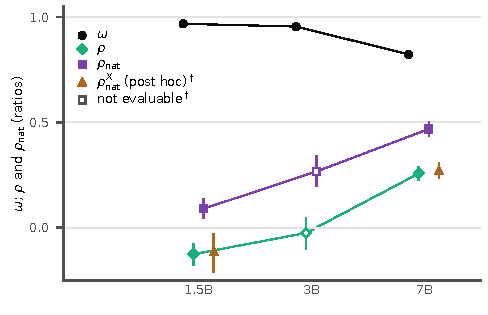
\includegraphics[width=0.5\textwidth]{figures/fig_flag_scale.pdf}
\caption{\textbf{The flag across scale} (Qwen2.5-1.5B, 3B and 7B; 95\,\% story-bootstrap intervals). $\omega$: how far the flag written in a sentence matches the list's; $\rho$ and $\rho_{\mathrm{nat}}$: the injected and the natural sentence-to-list ratio (J-D6, not met: outcome ``Mixed.''); $\rho^X_{\mathrm{nat}}$: the natural ratio on the contrast specific to the absent option (post hoc). Hollow and $\dagger$: not evaluable at 3B, values recomputed.}
\label{fig:flag-scale}
\end{figure}

\paragraph{The flag is written in sentences (J-D6a, replication, held).} At Qwen2.5-1.5B, 3B and 7B the flag written by the reader heads at the sentence's re-mentions matches the list's: $\omega$ = \JdSixaOmegaQwenOnefive{}, \JdSixaOmegaQwenThree{} and \JdSixaOmegaQwenSeven{}, cosine $c_{\mathrm{fl}}$ = \JdSixaKappaQwenOnefive{}, \JdSixaKappaQwenThree{} and \JdSixaKappaQwenSeven{} (\cref{tab:flag}, bottom). The sentence flag injected at the list row moves the answer \JdSixbQwenOnefive{}, \JdSixbQwenThree{} and \JdSixbQwenSeven{} as much as the list flag (reported). The reader heads at 1.5B and 3B were ranked in the final round with the discovery sample's procedure (17 and 29 heads).

\paragraph{Mediation (J-D6, risky, not held; J-D6-ROUTE, risky, not held).} J-D6 predicted that the list flag injected at the sentence's row of the absent option reproduces the natural ratio of the sentence read to the list read, in sign and within $\pm\max(0.1, 0.5\lvert\rho_{\mathrm{nat}}\rvert)$. At 1.5B the signs differ ($\rho$ = \JdSixRhoQwenOnefive{} [\JdSixRhoQwenOnefiveLo{}, \JdSixRhoQwenOnefiveHi{}] against $\rho_{\mathrm{nat}}$ = \JdSixRhoNatQwenOnefive{} [\JdSixRhoNatQwenOnefiveLo{}, \JdSixRhoNatQwenOnefiveHi{}]); at 7B $\rho$ = \JdSixRhoQwenSeven{} against $\rho_{\mathrm{nat}}$ = \JdSixRhoNatQwenSeven{}, a difference of \JdSixDiffQwenSeven{} [\JdSixDiffQwenSevenLo{}, \JdSixDiffQwenSevenHi{}] against a tolerance of $\pm$\JdSixTolQwenSeven{}; 3B is not evaluable (\JdGsixCompQwenThree{} of \JdGsixNQwenThree{} competent cores, against 40). J-D6-ROUTE predicted that at 1.5B the injected flag is read by value under \fmtPost{}; it is read by key ($r^{\mathrm{inj}}(V)$ = \JdSixRouteVQwenOnefive{}, $r^{\mathrm{inj}}(K)$ = \JdSixRouteKQwenOnefive{}, difference \JdSixRouteVmKQwenOnefive{} [\JdSixRouteVmKQwenOnefiveLo{}, \JdSixRouteVmKQwenOnefiveHi{}]). The preregistered decision table gives outcome (\JdSixTable{}), whose text is ``Mixed.'': J-D6 is not met, and $\rho_{\mathrm{nat}}$ is positive in both evaluable models, so the outcome ``not mediated'' does not apply. % verbatim: D6 decision table, entry J part D

\paragraph{A post hoc reading of the natural ratio.} The preregistered $\rho_{\mathrm{nat}}$ divides the natural clamp's effect on X under \fmtPost{} by that under \fmtOpt{}; under \fmtPost{} it includes a gain that every candidate other than B gets when B loses its key match (at 1.5B the clamp to S raises X more than the clamp to X does). On a contrast specific to the absent option (the clamp to X minus the clamp to S, on X), the natural ratio is \JdSixNatXQwenOnefive{} [\JdSixNatXQwenOnefiveLo{}, \JdSixNatXQwenOnefiveHi{}] at 1.5B and \JdSixNatXQwenSeven{} [\JdSixNatXQwenSevenLo{}, \JdSixNatXQwenSevenHi{}] at 7B, and $\rho$ minus it is \JdSixDiffXQwenOnefive{} [\JdSixDiffXQwenOnefiveLo{}, \JdSixDiffXQwenOnefiveHi{}] and \JdSixDiffXQwenSeven{} [\JdSixDiffXQwenSevenLo{}, \JdSixDiffXQwenSevenHi{}]; on the ratio of $\mathrm{ID}_K$, from which the entry's prior was taken, it is \JdSixNatIDKQwenOnefive{} and \JdSixNatIDKQwenSeven{}, and $\rho$ minus it \JdSixDiffIDKQwenOnefive{} [\JdSixDiffIDKQwenOnefiveLo{}, \JdSixDiffIDKQwenOnefiveHi{}] and \JdSixDiffIDKQwenSeven{} [\JdSixDiffIDKQwenSevenLo{}, \JdSixDiffIDKQwenSevenHi{}] (post hoc, recomputed). On these contrasts the injected sentence-row flag reproduces the natural ratio in sign and size, and the decision table would read (b). This reading came after the data and cannot be scored: the verdict stays not met and the outcome (d), and we draw no conclusion about mediation from it in either direction. At 3B, on its 35 competent cores, the line would have failed: $\rho$ = \JdSixRhoQwenThree{} against $\rho_{\mathrm{nat}}$ = \JdSixRhoNatQwenThree{} (post hoc, recomputed). % verbatim: 35 cores, outcome J part D

\clearpage
% Appendix F: details of Claim 3 (where an intervention appears to act). Input by sections/appendix.tex.
\section{Where an intervention appears to act: details}\label{app:claim3}

This appendix gives the design and every result of the final round's test of the channel-ratio law (preregistration J, part C): five families of identity edits obtained independently of the natural clamp, in Qwen2.5-7B, Mistral-7B and Llama-3.1-8B, on 80 new stories (\cref{app:prompts-intervention}). The motivating case, the released remap, is in \cref{app:remap}; the binding swap at block 28 and the overlap screen are in \cref{app:binding-j}. % verbatim: 80 stories, entry J part C

\subsection{The law, the lemma and the statistics}\label{app:law}

\paragraph{The law.} For an edit $Z$ that writes a value at the writing token at depth $l$ (the output of 0-based block $l$), channel $C \in \{K, V, KV\}$ and format $f$, let $\psi_C^Z(f, l) = \overline{\mathrm{ID}}{}_C^Z / \overline{\mathrm{ID}}{}_C^{\mathrm{nat}}$ be the edit's identity effect through channel $C$ as a share of the natural write's, from block $l{+}1$ on. The channel-ratio law states that one scaling per edit holds for both channels and in every format: $\psi_K^Z = \psi_V^Z$. Its statistic is $\lambda = \log(\psi_K/\psi_V)$ (\cref{sec:claim3}; each $\psi$ floored at 0.01, so that a dead channel is a departure), computed in three ways at each depth: $W(f, l)$ within one format, for \fmtOpt{} and \fmtPost{} where both channels are used; $A_L(l)$, the key read under \fmtLetter{} against the value read under \fmtNone{}; and $A_P(l)$, the key read under \fmtOpt{} against the value read under \fmtNone{}. A channel is used in a cell when its natural identity effect is at least 2 nats and at least a tenth of the joint effect. A statistic is equivalent when its 90\,\% interval lies inside $\pm\log 1.25$ (two one-sided tests at 5\,\%); it counts as a departure when the edit's key and value effects interact (its interaction $\iota_{KV} > 0.5$ in one of its cells; not the $\iota$ of \cref{app:flag}). The law holds in a combination of model, edit and depths (a combo) when it has at least three statistics and every one is equivalent; otherwise the combo's pattern is copy-only (rival R1: pooled $\bar\lambda \leq \log 0.5$), key-flat (R3: $\bar\lambda \geq \log 2$) or a graded departure. A line over several combos holds only if every evaluable combo holds (an intersection-union test).

\paragraph{The lemma.} Because the base and source prompts differ only at the writing token $p$, an edit confined to the residual at $(p, l)$ reaches every other position only through $p$'s keys and values in blocks $\geq l{+}1$: under the causal mask $p$'s residual reaches other tokens only through attention, and $p$'s keys and values in blocks $\leq l$ are computed from inputs the edit does not change. So the base run with the edit's keys and values written at $p$ from block $l{+}1$ is exactly the edited run, and its key-only and value-only rows are exact. Writing the source run's residual $h_{\mathrm{S},l}(p)$ gives the source's keys and values at $p$ from $l{+}1$: this edit is the natural clamp itself. Every edit is therefore applied as a clamp row whose tables come from a prefix pass with the edit written; the prefix through $p$ is the same in all four formats, so an edit's tables are the same tensors in every format and only the readers after $p$ differ. The unit tests check the lemma in FP32 to $10^{-4}$.

\paragraph{Controls of the design.} The natural write written as an edit (T) is the equivalence control: its tables and rows equal the natural ones bitwise in every evaluable cell of all three models (\JcGoneCellsQwenSeven{} cells each), so every statistic of T is equivalent. A sensitivity gate checked that the statistics can see a departure: synthetic rows whose key table is interpolated halfway toward the base run (SK50) were classified as copy-only ($\bar\lambda$ = \JcGeightSkFiftyQwenSeven{}, \JcGeightSkFiftyMistralSeven{} and \JcGeightSkFiftyLlamaEight{}), and rows with the value table halved (SV50) as graded departures (\JcGeightSvFiftyQwenSeven{}, \JcGeightSvFiftyMistralSeven{}, \JcGeightSvFiftyLlamaEight{}). The design's earlier key-share rule ($\kappa = K/(K+V)$ within a margin of the natural share) passes SV50, a two-fold channel departure: this compression is why the law is stated on log ratios. The natural format effect on the key share is large in all three models ($\sigma(\text{\fmtLetter{}}, 3) - \sigma(\text{\fmtNone{}}, 3)$ = \JcGtwoQwenSeven{}, \JcGtwoMistralSeven{} and \JcGtwoLlamaEight{}). Intervals of the law are 90\,\% hierarchical bootstrap intervals over the 24 ordered base--source pairs and the stories within them (with the remap's two seeds as a further level); others are 95\,\%. % verbatim: entry J part C

\subsection{The edit families and their gates}\label{app:edits}

\paragraph{Families.} Each edit writes, at $(p, l)$ for $l \in \{3, 7, 11, 15\}$, a target value $t$ (S or X) in place of B:
\begin{itemize}\setlength\itemsep{0pt}
  \item \textbf{E1}, in-task steering vectors: $h_{\mathrm{B}} + \mu_1(t) - \mu_1(\mathrm{B})$, with $\mu_1(x)$ the mean residual at $(p, l)$ over 150 held-out stories with $x$ written \citep{turner2023actadd,panickssery2023caa};
  \item \textbf{E2}, steering vectors from unrelated sentences: the same with $\mu_2(x)$, the mean block-$l$ output at the token of $x$ over 24 neutral sentences;
  \item \textbf{E3}, features of a public sparse autoencoder (Qwen2.5-7B only): the BatchTopK dictionaries of \citet{andyrdt2025saes} \citep{bussmann2024batchtopk} at layers 3, 7, 11 and 15, at a pinned revision; the edit sets the latents most selective for $t$ to their mean on stories with $t$ written and removes those selective for B, leaving every other latent and the reconstruction error at B's; the number of latents (\JcGthreeKfThree{} at every layer) was set on calibration stories;
  \item \textbf{E4}, a remap trained at the writing token: a rank-16 distributed alignment search basis fitted at $(p, l)$ with the released training recipe of \citet{anonymous2026fitted} (pair-swap objective, six-way cross-entropy, one epoch over 1{,}000 training stories, two seeds, one from the PCA basis and one random), without a later mention; its losses fell from \JcDasLossFirstMin{}--\JcDasLossFirstMax{} to \JcDasLossLastMin{}--\JcDasLossLastMax{} and its held-out flip rates are \JcDasFlipMin{}--\JcDasFlipMax{};
  \item \textbf{E5}, the boundary family: steering vectors that write $t$ as its French (FR) or German (DE) word or a synonym (SYN), and the part of E1 outside the English lexical span (NL); scaled by 1 or 2 on calibration stories.
\end{itemize}
Each edit's displacement is split into its component along the story's natural displacement (PAR) and the rest (PERP), and into its projection on the five-dimensional span of the English candidate words' mean residuals (LEX) and the rest (NONLEX). A component carries identity when its effect without a later mention is at least 0.3 of the natural one with a lower bound above zero. The distance $\nu$ of an edit's cached keys and values from the natural ones, relative to the natural displacement, is reported per cell (post hoc use in \cref{app:nu}). % verbatim: entry J part C

\paragraph{Gates.} The FP32 tests passed (95 tests). T reproduced the natural tables in every evaluable cell; the natural format effect held; the sensitivity gate held in all three models. The cell gate (natural joint effect at least 2 nats, interaction at most 0.5, coverage at least 0.8) failed in \JcGfourFail{} of 48 cells: \fmtLetter{} at blocks 11 and 15 in every model, where the natural effect is small. The efficacy gate (flip rate at least 0.8 of the natural and $\varphi$ above 0.5 without a mention) held for E1 and E2 at every depth in all three models ($\varphi$ \JcGfivePhiNearMin{}--\JcGfivePhiNearMax{}) and for E3 at all four layers (\JcGfivePhiEthreeMin{}--\JcGfivePhiEthreeMax{}); E4 is effective at blocks 3 and 7 at Qwen2.5-7B and 3, 7 and 11 at Mistral-7B ($\varphi$ \JcGfivePhiEfourEffMin{}--\JcGfivePhiEfourEffMax{}) and not deeper; the E5 sub-families are mostly ineffective. Random directions of the natural norm move nothing beyond the specificity bound at any depth. % verbatim: outcome J part C

\paragraph{The dictionary gate failed through its specification.} The gate required each dictionary's fraction of variance explained (FVE) on its block's outputs, over every prompt position after the first, to be within 0.05 of its published value. It failed at all four layers (FVE $\JcGthreeFveRoundThree$, $\JcGthreeFveRoundSeven$, $\JcGthreeFveRoundEleven$ and $\JcGthreeFveRoundFifteen$ against published values of \JcGthreePubRoundThree{}, \JcGthreePubRoundSeven{}, \JcGthreePubRoundEleven{} and \JcGthreePubRoundFifteen{}), so E3 is not evaluable in every line that uses it. The published FVE is computed after the dictionary's training buffer drops the first tokens of each sample and activations with norms above ten times the batch median; the gate dropped only the first position and kept the chat template's tokens, identical in all prompts, where large-norm activations appear from block 3 on (inferred: the layer-3 dictionary explains \JcGthreeFvePrevThree{} of the variance on block 2 and fails on block 3; the per-position activations were not saved). At the writing position the layer-3 dictionary reproduces its published value (FVE \JcGthreeFvePThree{} against \JcGthreePubRoundThree{}), and E3 flips every answer at every layer. The gate measured reconstruction over positions that the dictionary's published fit excludes; a corrected gate needs a rerun. After the data (post hoc, recomputed): admitting only layer 3, whose FVE at the writing position is within 0.05 of the published value, the E3 law would not hold (\JcThreePosthocLayerThreeNeq{} of \JcThreePosthocLayerThreeNstat{} statistics equivalent, $\bar\lambda$ = \JcThreePosthocLayerThreePool{}); admitting all four layers, \JcThreePosthocAllNeq{} of \JcThreePosthocAllNstat{}; no component of E3 carries identity. These statistics appear in \cref{tab:law,fig:nu} marked post hoc. % verbatim: outcome J part C

\subsection{Results per line}\label{app:lawresults}

\begin{table}[!ht]
\centering
\caption{\textbf{Every $\lambda$ statistic of the channel-ratio law.} $\lambda = \log\psi_K - \log\psi_V$ with its 90\,\% hierarchical bootstrap interval, per model, edit and depth $l$; $W(\cdot, l)$ within \fmtOpt{} (first column) or \fmtPost{}; $A_L(l)$ and $A_P(l)$: the key read under \fmtLetter{} or \fmtOpt{} against the value read under \fmtNone{}. $^{*}$Not equivalent (the interval is not inside $\pm\log 1.25 = \pm 0.223$); $^{\iota}$a departure by the interaction rule ($\iota_{KV} > 0.5$); --: a cell not used or not evaluable. Line: the line the statistic belongs to (n.e.: in a combo with fewer than three statistics). $^\dagger$Recomputed through the scorer's code, not printed by it (post hoc): E3, whose layers fail the dictionary gate; the E5 sub-families, whose line prints only pooled values; Qwen2.5-7B E2 at $l = 11$.}
\label{tab:law}
\resizebox{\textwidth}{!}{\footnotesize
\setlength{\tabcolsep}{3pt}
\begin{tabular}{@{}lllcccc l@{}}
\toprule
Model & Edit & $l$ & $W(\mathrm{P1}, l)$ & $W(\mathrm{POST}, l)$ & $A_L(l)$ & $A_P(l)$ & Line \\
\midrule
Qwen2.5-7B & E1 & 3 & $-$0.02 [$-$0.03, $-$0.02] & $-$0.02 [$-$0.03, 0.00] & 0.00 [$-$0.01, 0.00] & $-$0.02 [$-$0.03, $-$0.02] & J-C1 \\
 &  & 7 & $-$0.06 [$-$0.08, $-$0.03] & $-$0.11 [$-$0.15, $-$0.07] & $-$0.05 [$-$0.07, $-$0.03] & $-$0.07 [$-$0.10, $-$0.05] & J-C1 \\
 &  & 11 & $-$0.16 [$-$0.25, $-$0.08]$^{*\iota}$ & -- & -- & $-$0.18 [$-$0.27, $-$0.11]$^{*\iota}$ & J-C1 \\
 & E2 & 3 & $-$0.01 [$-$0.03, 0.01] & 0.05 [0.02, 0.08] & 0.00 [$-$0.02, 0.01] & 0.02 [0.00, 0.04] & J-C1 \\
 &  & 7 & $-$0.14 [$-$0.19, $-$0.10] & $-$0.22 [$-$0.31, $-$0.16]$^{*}$ & $-$0.15 [$-$0.21, $-$0.11] & $-$0.11 [$-$0.15, $-$0.07] & J-C1 \\
 &  & 11 & $-$0.27 [$-$0.39, $-$0.17]$^{*}$ & -- & -- & $-$0.21 [$-$0.34, $-$0.11]$^{*}$ & J-C2 (n.e.) \\
 & E3$^\dagger$ & 3 & $-$0.17 [$-$0.23, $-$0.12]$^{*}$ & $-$0.23 [$-$0.30, $-$0.17]$^{*}$ & $-$0.09 [$-$0.15, $-$0.04] & $-$0.19 [$-$0.25, $-$0.14]$^{*}$ & post hoc \\
 &  & 7 & $-$0.71 [$-$0.89, $-$0.55]$^{*}$ & $-$1.40 [$-$2.07, $-$1.03]$^{*}$ & $-$0.71 [$-$0.91, $-$0.55]$^{*}$ & $-$0.79 [$-$0.94, $-$0.65]$^{*}$ & post hoc \\
 &  & 11 & $-$1.01 [$-$1.26, $-$0.82]$^{*}$ & -- & -- & $-$1.10 [$-$1.36, $-$0.91]$^{*}$ & post hoc \\
 & E4 & 3 & $-$0.70 [$-$0.92, $-$0.49]$^{*}$ & $-$2.01 [$-$4.31, $-$1.31]$^{*}$ & $-$0.67 [$-$0.92, $-$0.46]$^{*}$ & $-$0.74 [$-$0.95, $-$0.55]$^{*}$ & J-C4 \\
 &  & 7 & $-$1.47 [$-$1.87, $-$1.15]$^{*\iota}$ & $-$3.17 [$-$4.23, $-$2.25]$^{*}$ & $-$2.09 [$-$3.17, $-$1.55]$^{*\iota}$ & $-$1.74 [$-$2.16, $-$1.41]$^{*\iota}$ & J-C4 \\
 & E4, seed 101 & 3 & $-$0.80 [$-$1.00, $-$0.63]$^{*}$ & $-$3.10 [$-$4.35, $-$2.07]$^{*}$ & $-$0.73 [$-$0.98, $-$0.53]$^{*}$ & $-$0.78 [$-$0.99, $-$0.60]$^{*}$ & J-C4 (seed) \\
 & E4, seed 102 & 3 & $-$0.59 [$-$0.80, $-$0.42]$^{*}$ & $-$1.50 [$-$1.96, $-$1.18]$^{*}$ & $-$0.61 [$-$0.87, $-$0.39]$^{*}$ & $-$0.70 [$-$0.93, $-$0.51]$^{*}$ & J-C4 (seed) \\
 &  & 7 & $-$1.30 [$-$1.63, $-$1.05]$^{*\iota}$ & $-$3.70 [$-$4.28, $-$2.41]$^{*}$ & $-$1.77 [$-$2.30, $-$1.40]$^{*\iota}$ & $-$1.59 [$-$1.93, $-$1.31]$^{*\iota}$ & J-C4 (seed) \\
 &  & 11 & $-$1.30 [$-$1.73, $-$1.02]$^{*}$ & -- & -- & $-$1.59 [$-$2.04, $-$1.29]$^{*}$ & J-C4 (seed) \\
 & PERP of E4 & 3 & $-$1.70 [$-$2.09, $-$1.39]$^{*}$ & -- & -- & $-$1.77 [$-$2.22, $-$1.41]$^{*}$ & J-C5 \\
 & NONLEX of E4 & 3 & $-$1.77 [$-$2.11, $-$1.47]$^{*}$ & -- & -- & $-$1.88 [$-$2.23, $-$1.58]$^{*}$ & J-C5 \\
 &  & 7 & $-$1.97 [$-$2.63, $-$1.52]$^{*}$ & -- & -- & $-$2.37 [$-$3.03, $-$1.92]$^{*}$ & J-C5 \\
 & E5-NL$^\dagger$ & 11 & $-$0.58 [$-$1.08, $-$0.27]$^{*}$ & -- & -- & $-$0.83 [$-$1.34, $-$0.51]$^{*}$ & J-C-BOUND \\
\midrule
Mistral-7B & E1 & 3 & -- & $-$0.02 [$-$0.03, $-$0.01] & 0.00 [$-$0.01, 0.01] & $-$0.01 [$-$0.02, 0.00] & J-C1 \\
 &  & 7 & -- & $-$0.19 [$-$0.27, $-$0.13]$^{*}$ & $-$0.06 [$-$0.12, $-$0.03] & $-$0.08 [$-$0.16, $-$0.04] & J-C1 \\
 & E2 & 3 & -- & 0.01 [0.00, 0.02] & 0.00 [0.00, 0.01] & 0.00 [$-$0.01, 0.02] & J-C1 \\
 &  & 7 & -- & $-$0.22 [$-$0.35, $-$0.13]$^{*}$ & $-$0.18 [$-$0.27, $-$0.11]$^{*}$ & $-$0.15 [$-$0.29, $-$0.07]$^{*}$ & J-C1 \\
 & E4 & 3 & -- & $-$0.93 [$-$1.42, $-$0.62]$^{*}$ & $-$0.55 [$-$0.90, $-$0.29]$^{*}$ & $-$0.54 [$-$0.93, $-$0.31]$^{*}$ & J-C4 \\
 &  & 7 & -- & $-$3.92 [$-$4.24, $-$1.96]$^{*}$ & $-$1.95 [$-$2.78, $-$1.49]$^{*}$ & $-$2.36 [$-$3.87, $-$1.82]$^{*}$ & J-C4 \\
 & E4, seed 101 & 7 & -- & $-$2.63 [$-$4.02, $-$1.69]$^{*}$ & $-$1.90 [$-$2.50, $-$1.48]$^{*}$ & $-$2.53 [$-$3.92, $-$1.96]$^{*}$ & J-C4 (seed) \\
 & E4, seed 102 & 3 & -- & $-$0.83 [$-$1.25, $-$0.54]$^{*}$ & $-$0.44 [$-$0.71, $-$0.22]$^{*}$ & $-$0.44 [$-$0.67, $-$0.27]$^{*}$ & J-C4 (seed) \\
 &  & 7 & -- & $-$4.22 [$-$4.27, $-$2.58]$^{*}$ & $-$1.99 [$-$3.16, $-$1.47]$^{*}$ & $-$2.23 [$-$3.52, $-$1.70]$^{*}$ & J-C4 (seed) \\
 & PERP of E4 & 3 & -- & -- & -- & $-$1.91 [$-$3.28, $-$1.31]$^{*}$ & J-C5 \\
 &  & 7 & -- & -- & -- & $-$3.30 [$-$3.46, $-$3.10]$^{*}$ & J-C5 \\
 & NONLEX of E4 & 3 & -- & -- & -- & $-$1.19 [$-$2.08, $-$0.72]$^{*}$ & J-C5 \\
 &  & 7 & -- & -- & -- & $-$2.02 [$-$3.17, $-$1.57]$^{*}$ & J-C5 \\
 & E5-FR$^\dagger$ & 7 & -- & $-$0.35 [$-$0.88, 0.06]$^{*}$ & $-$0.33 [$-$0.67, 0.01]$^{*}$ & $-$0.05 [$-$0.52, 0.32]$^{*}$ & J-C-BOUND \\
 & E5-NL$^\dagger$ & 7 & -- & $-$1.82 [$-$3.45, $-$1.11]$^{*}$ & $-$0.33 [$-$0.59, $-$0.12]$^{*}$ & $-$0.27 [$-$0.78, 0.01]$^{*}$ & J-C-BOUND \\
\midrule
Llama-3.1-8B & E1 & 3 & $-$0.01 [$-$0.02, 0.00] & $-$0.05 [$-$0.07, $-$0.04] & $-$0.03 [$-$0.04, $-$0.02] & $-$0.02 [$-$0.03, $-$0.01] & J-C2 \\
 &  & 7 & $-$0.06 [$-$0.09, $-$0.03] & -- & $-$0.08 [$-$0.12, $-$0.05] & $-$0.08 [$-$0.11, $-$0.06] & J-C2 \\
 & E2 & 3 & $-$0.01 [$-$0.04, 0.01] & $-$0.01 [$-$0.03, 0.01] & $-$0.03 [$-$0.04, $-$0.02] & $-$0.02 [$-$0.04, $-$0.01] & J-C2 \\
 &  & 7 & $-$0.24 [$-$0.30, $-$0.18]$^{*}$ & -- & $-$0.32 [$-$0.42, $-$0.24]$^{*}$ & $-$0.26 [$-$0.34, $-$0.20]$^{*}$ & J-C2 \\
 & PERP of E2 & 7 & $-$1.47 [$-$2.12, $-$1.06]$^{*}$ & -- & -- & $-$1.75 [$-$2.41, $-$1.34]$^{*}$ & J-C5 \\
 & E5-FR$^\dagger$ & 7 & $-$0.50 [$-$0.83, $-$0.24]$^{*}$ & -- & $-$0.55 [$-$0.85, $-$0.27]$^{*}$ & $-$0.62 [$-$0.90, $-$0.40]$^{*}$ & J-C-BOUND \\
 & E5-SYN$^\dagger$ & 3 & $-$0.78 [$-$1.05, $-$0.57]$^{*}$ & $-$0.01 [$-$0.37, 0.30]$^{*}$ & $-$1.92 [$-$2.35, $-$1.58]$^{*}$ & $-$1.02 [$-$1.35, $-$0.75]$^{*}$ & J-C-BOUND \\
 &  & 7 & $-$0.87 [$-$1.11, $-$0.68]$^{*}$ & -- & $-$1.82 [$-$2.27, $-$1.48]$^{*}$ & $-$1.04 [$-$1.35, $-$0.76]$^{*}$ & J-C-BOUND \\
 & E5-NL$^\dagger$ & 7 & $-$1.09 [$-$1.46, $-$0.78]$^{*}$ & -- & $-$0.50 [$-$0.78, $-$0.29]$^{*}$ & $-$1.10 [$-$1.45, $-$0.81]$^{*}$ & J-C-BOUND \\
\bottomrule
\end{tabular}
}
\end{table}

\paragraph{Steering vectors (J-C1, not held; J-C2, not held).} J-C1 (extrapolation) required every statistic of E1 at every depth and of E2 at blocks 3 and 7 to be equivalent at Qwen2.5-7B and Mistral-7B. Equivalent were \JcOneNeqEoneQwenSeven{} of \JcOneNstatEoneQwenSeven{} statistics of E1 at Qwen ($\bar\lambda$ = \JcOnePoolEoneQwenSeven{}), \JcOneNeqEoneMistralSeven{} of \JcOneNstatEoneMistralSeven{} at Mistral (\JcOnePoolEoneMistralSeven{}), \JcOneNeqEtwoQwenSeven{} of \JcOneNstatEtwoQwenSeven{} of E2 at Qwen (\JcOnePoolEtwoQwenSeven{}) and \JcOneNeqEtwoMistralSeven{} of \JcOneNstatEtwoMistralSeven{} at Mistral (\JcOnePoolEtwoMistralSeven{}): graded departures, every pooled $\bar\lambda$ within the margin but not every statistic. The line's pre-written sentence (the main text opens instead with the outcome text below; \cref{app:decisions}): ``Even steering vectors close to the natural edit depart from the natural channel ratio ($\bar\lambda$ = \JcOnePoolEoneMistralSeven{} to \JcOnePoolEtwoMistralSeven{}): the format law does not transfer to edits as a channel-ratio law.'' J-C2 (extrapolation) covered E2 at blocks 11 and 15 (not evaluable at Qwen and Mistral: \JcTwoNstatEtwoQwenSeven{} and \JcTwoNstatEtwoMistralSeven{} statistics) and Llama-3.1-8B: E1 held there (\JcTwoNeqEoneLlamaEight{} of \JcTwoNstatEoneLlamaEight{} equivalent, $\bar\lambda$ = \JcTwoPoolEoneLlamaEight{}), E2 did not (\JcTwoNeqEtwoLlamaEight{} of \JcTwoNstatEtwoLlamaEight{}, $\bar\lambda$ = \JcTwoPoolEtwoLlamaEight{}). Every failing statistic is a key under-read at block 7 or deeper (\cref{tab:law}). % verbatim: J-C1 text, outcome J part C

\paragraph{Where the steering vectors depart (post hoc).} In the core test (J-C1), \JcOneCoreNe{} of its \JcOneCoreN{} $\lambda$ statistics are not equivalent, all at block \JcOneCoreNeDepthMin{} or deeper, and the number of them with a 90\,\% interval wholly outside the margin is \JcOneCoreNeOut{}: each failure is an inconclusive test rather than a shown departure, and all but one point estimate lie inside the margin (recomputed). A rule that requires every one of six to ten statistics to be equivalent has limited power against a small, consistent under-read: the entry's power analysis, seen before finalisation, expected the criterion to accept key-to-value imbalances up to about 0.9 and to reject 0.8 and beyond, and the pooled ratios $e^{\bar\lambda}$ of the core test are \fpeval{round(exp(\JcOnePoolEtwoMistralSeven),2)}--\fpeval{round(exp(\JcOnePoolEoneMistralSeven),2)} (arithmetic on the printed values). At Llama-3.1-8B, \JcTwoLlamaEtwoNe{} statistics of the vectors from unrelated sentences are not equivalent and \JcTwoLlamaEtwoNeOut{} lies wholly outside the margin (J-C2). Every non-equivalent E1 or E2 statistic is a key-channel under-read ($\psi_K$ \JcOneNePsiKMin{}--\JcOneNePsiKMax{} with $\psi_V$ \JcOneNePsiVMin{}--\JcOneNePsiVMax{}) in a cell whose natural key identity effect is small, \JcOneNeIDKMin{}--\JcOneNeIDKMax{} nats (natural key shares \JcOneNeShareSmallMin{}--\JcOneNeShareSmallMax{} in the cells of the sentence after the story and of Qwen's \fmtOpt{} cell at block 11, and 0.47--\JcOneNeShareMax{} in the block-7 cells with lettered options or options after of Mistral-7B and Llama-3.1-8B), against natural value effects of 5.8 to \JcOneNeIDVMax{} nats, except in Llama-3.1-8B's \fmtOpt{} cell at block 7, whose value effect (\JcOneNeIDVMin{} nats) is smaller than its key effect (exploratory, recomputed). % verbatim: "0.47--0.81" and "5.8", outcome J part C At block 3 every statistic of the three models is equivalent ($\lvert\lambda\rvert \leq$ \JcOneLamThreeAbsMax{}; exploratory). At block 7 the key under-read is also present where the natural key effect is large, but inside the margin (Qwen E2 $A_L(7)$: $\lambda$ = \JcOneEtwoAletterSevenLamQwenSeven{}, $\psi_K$ = \JcOneEtwoAletterSevenPsiKQwenSeven{} at \JcOneEtwoAletterSevenIDKQwenSeven{} nats; post hoc). Pooled over depths, the keys under-read the steering vectors by 4.5--12\,\% ($\bar\lambda$ \JcTwoPoolEoneLlamaEight{} to \JcTwoPoolEtwoLlamaEight{}). After the data, a channel floor of 4.8 nats in place of the preregistered 2 would make J-C1 met (all \JcOneFloorFourEightMet{} combos) and the headline outcome (d); floors of 3 and 4 nats leave it not met, and under the lower-case score J-C1 stays not met (post hoc, recomputed). This floor is not used. % verbatim: "4.5--12 %", outcome J part C

\paragraph{Sparse-autoencoder features (J-C3, risky, not evaluable).} Not evaluable through the dictionary gate (\cref{app:edits}); under either gate considered after the data the line would not have been met (post hoc, recomputed; \cref{app:edits}).

\paragraph{The remap trained at the writing token (J-C4, risky, not held).} No statistic of E4 is equivalent; the pooled $\bar\lambda$ is \JcFourPoolEfourQwenSeven{} [\JcFourPoolEfourQwenSevenLo{}, \JcFourPoolEfourQwenSevenHi{}] at Qwen2.5-7B and \JcFourPoolEfourMistralSeven{} [\JcFourPoolEfourMistralSevenLo{}, \JcFourPoolEfourMistralSevenHi{}] at Mistral-7B, copy-only (R1) in both models, for both seeds (per seed \JcFourPoolEfouraQwenSeven{} and \JcFourPoolEfourbQwenSeven{} at Qwen, \JcFourPoolEfouraMistralSeven{} and \JcFourPoolEfourbMistralSeven{} at Mistral) and under the lower-case score. The seed level of the hierarchical bootstrap rests on two seeds and cannot estimate seed variance; the per-seed values are given for that reason. The pre-written R1 sentence, used for the remap only: ``Edits that change the value through a learned remap are read mainly through the value ($\bar\lambda$ = \JcFourPoolEfourQwenSeven{} / \JcFourPoolEfourMistralSeven{}): the key channel does not read them as it reads the written word.'' Its size depends on depth (post hoc, recomputed): at block 3 alone $\bar\lambda$ is $\JcFourDepthThreeQwenSeven$ at Qwen and $\JcFourDepthThreeMistralSeven$ at Mistral (a graded departure), and at block 7 $\JcFourDepthSevenQwenSeven$ and $\JcFourDepthSevenMistralSeven$, where the statistics under \fmtPost{} sit near the floor of $\psi$ ($\psi_K$ = \JcFourPsiKWpostSevenQwenSeven{} and \JcFourPsiKWpostSevenMistralSeven{} against $\psi_V$ = \JcFourPsiVWpostSevenQwenSeven{} and \JcFourPsiVWpostSevenMistralSeven{}); we therefore quote $\psi_K$ and $\psi_V$ beside the pooled magnitudes, which the pre-written sentence fixes, and give them in the main text with the remap's key share at block 3 (\JcKappaEfouraOptThreeQwenSeven{} and \JcKappaEfourbOptThreeQwenSeven{} for the two seeds with the options after at Qwen2.5-7B, against the natural \JcSigmaOptThreeQwenSeven{}; reported). The remap does not act through the natural lexical code: its components along the natural displacement and along the lexical span carry at most \JcLexParShareEfourMax{} and \JcLexLexShareEfourMax{} of its effect, while E1 and E2 carry at least \JcLexCodeShareNearMin{} of theirs through one of them (reported). % verbatim: R1 text, outcome J part C

\paragraph{Identity-carrying components (J-C5, risky, not held).} \JcFiveCarriers{} PERP or NONLEX components of the effective edits carry identity without a mention ($\varphi$ \JcFivePhiMin{}--\JcFivePhiMax{}); \JcFiveCarriersStat{} of them have \JcFiveNstat{} statistics in all, between \JcFiveLamMin{} and \JcFiveLamMax{}, and \JcFiveNeq{} are equivalent: identity written outside the natural direction or outside the lexical span is read mainly through the value.

\paragraph{The lexical boundary (J-C-BOUND, risky, not held).} The line predicted that a non-lexical identity edit is under-read by the key channel ($\bar\lambda_{\mathrm{E5}} \leq \log 0.5$ with an upper bound below $\log 0.8$) where E2 at the same cells is not ($\bar\lambda \geq \log 0.8$). Of the \JcBoundVerd{} sub-families with a verdict, two met it, Mistral-7B NL ($\bar\lambda$ = \JcBoundNlMistralSeven{}; E2 \JcBoundEtwoNlMistralSeven{}) and Llama-3.1-8B SYN (\JcBoundSynLlamaEight{}; E2 \JcBoundEtwoSynLlamaEight{}), and four did not: Qwen2.5-7B NL (\JcBoundNlQwenSeven{}; E2 \JcBoundEtwoNlQwenSeven{}), Mistral-7B FR (\JcBoundFrMistralSeven{} [\JcBoundFrMistralSevenLo{}, \JcBoundFrMistralSevenHi{}]), Llama-3.1-8B FR (\JcBoundFrLlamaEight{}; E2 \JcBoundEtwoFrLlamaEight{}) and Llama-3.1-8B NL (\JcBoundNlLlamaEight{}; E2 \JcBoundEtwoNlLlamaEight{}). The boundary was not isolated (post hoc, recomputed): every E5 $\bar\lambda$ lies below E2's at the same cells, but the two NL failures come only from E2's own departure at those cells, the line stays not met without the E2 control (both FR sub-families fail by themselves), and Mistral NL's pass rests on one near-floor statistic. The effective E5 edits write far from the natural state (post hoc; $\nu$ \JcBoundNuMin{}--\JcBoundNuMax{}) and follow the same distance pattern as the remap and the components (\cref{app:nu}); FR, DE and SYN are mostly ineffective because (post hoc) they write displacements \JcBoundFrDeSynNormMin{}--\JcBoundFrDeSynNormMax{} times the natural norm, nearly orthogonal to it (cosine at most \JcBoundFrDeSynCosMax{}). The pre-written sentence for this outcome is contradicted by the numbers and has one slot for six values; we claim neither that the token-form account holds for edits nor that it is contradicted (\cref{app:decisions}). % verbatim: outcome J part C

\paragraph{Reader heads (J-C-READa, not held; J-C-READb, risky, not evaluable).} At \fmtOpt{} and block 7, J-C-READa required the discovery sample's reader heads in blocks after 7 (32 heads at Qwen, 43 at Mistral) % verbatim: entry J part C
 to remove at least 0.7 of each steering vector's key read when blinded, and three size-matched random sets at most 0.25 on average. The readers removed \JcReadaKOMin{}--\JcReadaKOMax{}, about what they remove of the natural write (\JcReadaKONatQwenSeven{} and \JcReadaKONatMistralSeven{}); the random sets removed \JcReadaRandMin{}--\JcReadaRandMax{}, and the line was not met. The random-set control fails for the natural value as well (post hoc, recomputed): the natural donor's random-set mean is \JcReadaRandNatQwenSeven{} at Qwen and \JcReadaRandNatMistralSeven{} at Mistral, and the edits match the natural donor within \JcReadaPairMax{} on the readers and on the random-set mean (Mistral E2 on the readers \JcReadaPairEtwoHMistralSeven{}, post hoc). The sets are size-matched among the heads of blocks after 7 (560 and 768 heads) but not drawn disjoint from the readers; at Qwen one of them contains the top-ranked reader and removes \JcReadaSetZeroNatQwenSeven{} of the natural read (post hoc). The bound of 0.25 was carried over from stage 6, whose sets were drawn from all blocks with the key clamped from block 0; the failure is of the control in this design, not evidence that other heads read the edits, and a criterion referred to the natural donor would make the line met (post hoc reading). J-C-READb (the same for E3 and E4) is not evaluable under the line's text: E3 through its gate, and E4 because its own key read at block 7 is below 2 nats (\JcReadbIDKEfouraQwenSeven{} and \JcReadbIDKEfouraMistralSeven{}). Under the common part's evaluability rule, by which a quantity the tested arm makes undefined counts against the line, it would be not met (E4's readers remove \JcReadbKOEfouraQwenSeven{} and \JcReadbKOEfouraMistralSeven{}, below 0.7, post hoc and recomputed), and the risky tally would read \JxRiskyMetABCDAlt{} of \JxRiskyVerdABCDAlt{} (expected \JxRiskyExpABCDAlt{}); the official verdict is used (\cref{app:decisions}). % verbatim: outcome J part C

\paragraph{The headline.} The scorer checks the pre-committed outcomes for Section 5 in the order (a), (a$'$), (c), (b), (e), (d), (f) and prints the first whose condition holds: outcome (\JcHeadline{}), ``\JcHeadlineWord{}''. Outcomes (a) and (a$'$) need J-C3 and J-C4, or J-C5, met (the law for the autoencoder features and the trained remap, or for the identity-carrying components); (c) needs J-C-BOUND met; (b) needs every effective edit to act through the natural lexical code and no component to carry identity, but the trained remap does not act through it (its parallel and lexical components carry at most \JcLexParShareEfourMax{} and \JcLexLexShareEfourMax{} of its effect) and \JcFiveCarriers{} components carry identity; (e) applies because J-C1 is not met. Its pre-committed text, which the main text uses verbatim: ``Even steering vectors close to the natural edit depart from the natural channel ratio; the format law describes the model's own written value and does not predict how an edit is attributed.'' The binding-swap lines (J-C6 met, J-C-SCREEN met, J-C-WIN not evaluable) are in \cref{app:binding-j}. % verbatim: C-12 (e), entry J part C

\paragraph{Holm sensitivity.} Over the \JcHolmN{} interval components of this part's risky lines with a verdict, Holm's step-down changes \JcHolmChanged{} decisions (one statistic of the remap at block 3 and three upper bounds of the boundary line) and no verdict.

\subsection{Post hoc and exploratory}\label{app:nu}

\begin{figure}[!ht]
\centering
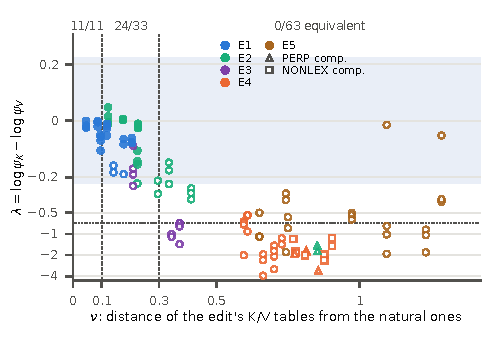
\includegraphics[width=0.62\textwidth]{figures/fig_nu.pdf}
\caption{\textbf{Post hoc: departures from the law follow how far an edit writes from the natural write.} Each point is one $\lambda$ statistic of an instance that carries identity ($\varphi$ without a mention at least 0.3), in the three models: full edits (circles; colour by family, E3 included although its gate failed) and PERP and NONLEX components (triangles, squares); filled: equivalent. $\nu$: the distance of the edit's cached keys and values from the natural ones, relative to the natural displacement. Band: $\pm\log 1.25$; dotted: $\log 0.5$, the copy-only bound; above the panel: equivalent of all statistics in each band of $\nu$ (cut-points chosen after the data). Linear $\nu$ axis; symmetric-log $\lambda$ axis, linear within $\pm 0.25$. Recomputed; post hoc.}
\label{fig:nu}
\end{figure}

\paragraph{Distance from the natural write (post hoc).} Over the \JcNuN{} $\lambda$ statistics of identity-carrying instances, $\lambda$ has Spearman correlation $\JcNuRhoNu$ with $\nu$ (95\,\% interval $\JcNuRhoNuLo$ to $\JcNuRhoNuHi$ from a bootstrap over the \JcNuUnits{} units of model, instance and depth, since each unit contributes several statistics) and \JcNuRhoCosK{} with the cosine of the edit's key displacement to the natural one; \JcNuEqLow{} of \JcNuNLow{} statistics with $\nu < 0.1$ are equivalent, \JcNuEqMid{} of \JcNuNMid{} with $\nu$ between 0.1 and 0.3, and \JcNuEqHigh{} of \JcNuNHigh{} beyond, of which \JcNuOutHigh{} have a 90\,\% interval wholly outside the margin (a shown departure) and the rest are inconclusive (\cref{fig:nu}). Four caveats limit the reading. (i)~The band cut-points 0.1 and 0.3 were chosen after the data. (ii)~At $\nu = 0$ the edit is the natural write and equivalence holds by construction, so a monotone association is partly guaranteed; only the rate of departure beyond small $\nu$ is informative. (iii)~$\nu$ is largely confounded with the edit family: of the \JcNuNBelow{} statistics with $\nu < 0.3$, \JcNuSteerBelow{} are steering vectors (E1, E2) and \JcNuEthreeBelow{} E3, while of the \JcNuNHigh{} beyond, \JcNuSteerAbove{} are steering vectors, \JcNuEthreeAbove{} E3 and \JcNuOtherAbove{} the remap, the non-lexical vectors and the components. Within the steering vectors ($n$ = \JcNuNSteer{}) the correlation is $\JcNuRhoSteer$; within the remap, non-lexical vectors and components ($n$ = \JcNuNOther{}) it is \JcNuRhoOther{}: beyond $\nu \approx 0.3$ every statistic comes from edits that are copy-read whatever their distance. (iv)~The table statistics are collinear (pairwise $\lvert$Spearman$\rvert$ \JcNuCollMin{}--\JcNuCollMax{} among $\nu$, the key, value and residual cosines and the first-order key projection), so $\nu$ cannot be told apart from the key cosine. The first-order prediction from the projections of the key and value displacements on the natural ones ranks the statistics only weakly (Spearman \JcOoneRho{}) and misses by $\JcOoneMiss$ on average: beyond $\nu \approx 0.3$ the key read collapses non-linearly while the value read decays more slowly (exploratory, recomputed). We therefore offer $\nu$ as a diagnostic to report alongside an intervention, not as an explanation of the departures. The pattern was found after the data and was not preregistered. A hypothesis for a future preregistration links it to the flag (\cref{app:flag}): the flag's dose response is threshold-like (half a flag barely moves the answer, one and two flags about equally), so the key route may select through a thresholded match while the value read degrades gradually; an edit that writes far from the natural state would then lose its key read first. It predicts that shrinking the key displacement of a near-natural steering vector past a threshold collapses $\psi_K$ while $\psi_V$ falls smoothly.

\paragraph{The key share against the natural share (reported).} At block 3 the steering vectors' key share is within 0.02 of the natural share in every format of all three models, while the remap's is lower. From block 3 to block 15 the change in the steering vectors' key share tracks the change in the natural share in \JcJcfourHold{} of \JcJcfourN{} qualifying pairs (largest gap \JcJcfourAbsMax{}), a consistency check that never enters the headline. % verbatim: "within 0.02", outcome J part C

\paragraph{Generated answers under the edits (exploratory).} At block 7, on the first 40 stories, E1 and E2 flip every generated answer without a mention in all three models, as the natural value does; with the options listed every edit flips fewer, the steering vectors at most as many as the natural value (natural value, E1, E2: \JcOfourOptNatQwenSeven{}, \JcOfourOptEoneQwenSeven{}, \JcOfourOptEtwoQwenSeven{} at Qwen2.5-7B; \JcOfourOptNatMistralSeven{}, \JcOfourOptEoneMistralSeven{}, \JcOfourOptEtwoMistralSeven{} at Mistral-7B; \JcOfourOptNatLlamaEight{}, \JcOfourOptEoneLlamaEight{}, \JcOfourOptEtwoLlamaEight{} at Llama-3.1-8B). The trained remap flips \JcOfourNoneEfouraQwenSeven{} / \JcOfourNoneEfouraMistralSeven{} and \JcOfourNoneEfourbQwenSeven{} / \JcOfourNoneEfourbMistralSeven{} of answers without a mention (two seeds; Qwen2.5-7B / Mistral-7B) but only \JcOfourOptEfouraQwenSeven{} / \JcOfourOptEfouraMistralSeven{} and \JcOfourOptEfourbQwenSeven{} / \JcOfourOptEfourbMistralSeven{} with the options listed: its key part, which the options' readers would need, is weak.

\clearpage
% Appendix G: the released remap. Input by sections/appendix.tex.
\section{The released remap}\label{app:remap}\label{sec:intervention}

This appendix describes, in our words, the intervention released with \citet{anonymous2026fitted} and everything we measured on it: the reproduction, the crossover across formats that motivates \cref{sec:claim3}, the refit without later mentions (preregistration F), the reader heads at 24B under the remap (preregistration I) and the same frames under the emitted-form score (final round). All of it is discovery sample except the last part. We describe what the released analysis does, not what its authors concluded from it.

\subsection{What the released analysis does}\label{app:remap-what}

The released analysis of \citet{anonymous2026fitted} patches Mistral-Small-24B and Qwen2.5-72B at the output of (1-based) decoder block 4 over every token of the event span (from ``\{$A$\} watches as'' to the end of the story). For a rank-16 basis $U$ with orthonormal rows, each span position becomes
\begin{equation}\label{eq:patch}
h \leftarrow h_{\mathrm{B}} + U^{\top} U\,(h_{\mathrm{S}} - h_{\mathrm{B}}).
\end{equation}
In the learned remap M, $U$ is a distributed alignment search basis \citep{geiger2024finding} fit with a six-choice cross-entropy objective so that the patched model ranks $\mathrm{T} = \pi(\mathrm{S})$ first, where $\pi$ is a fixed pair-swap of the six locations. In the control P, $U$ is an unfitted PCA basis of source-minus-base differences, which transfers S. We reuse the released bases (three seeds each; the Qwen2.5-72B PCA bases are reconstructions, labelled so by \citet{anonymous2026fitted}). Following the released design, a \emph{key-only exchange} replaces the writing token's key in every block from (1-based) block 6 on by the key of the other patched run, while queries, values and residual states evolve freely; we add the symmetric \emph{value-only exchange}. Unlike our clamp, these exchanges are not exact, because the patch also changes the other span tokens. With $m_{\mathrm{TS}} = \log p(\mathrm{T}) - \log p(\mathrm{S})$, writing $\mathrm{P}{+}K_{\mathrm{M}}$ for P with M's keys and $m(\cdot)$ for $m_{\mathrm{TS}}$ in a run,
\begin{align}
\varphi &= \frac{m(\mathrm{M}) - m(\mathrm{P})}{m(\mathrm{T}) - m(\mathrm{S})}, \label{eq:phi}\\
\psi_K &= \frac{m(\mathrm{P}{+}K_{\mathrm{M}}) - m(\mathrm{P})}{m(\mathrm{M}) - m(\mathrm{P})}, \label{eq:psik}\\
\psi_V &= \frac{m(\mathrm{P}{+}V_{\mathrm{M}}) - m(\mathrm{P})}{m(\mathrm{M}) - m(\mathrm{P})}. \label{eq:psiv}
\end{align}
$\varphi$ is the shift of M beyond P towards T, as a fraction of the natural S$\to$T shift; $\psi_K$ and $\psi_V$ are the fractions of the learned-minus-PCA difference that M's keys or values add to P. All are ratios of means over the 96 of their 120 native story cores in which B, S and T are distinct, after averaging the three fits within each core.

The exchanges are not exact, because the patch also changes the other span tokens; the removal fractions $\chi_K$ and $\chi_V$ and the implementation are in \cref{app:impl-clamps}. The remap was fit without the ``Answer:'' prefill of our formats, which the released analysis adds only at evaluation.

\subsection{Reproduction and the crossover across formats}\label{app:remap-crossover}

\paragraph{Reproduction.} Under \fmtOpt{}, the format of the released analysis, our runs of the released bases reproduce the released answers: the argmax of M and of P agrees with the released outputs on 0.994--1.000 of (core, fit) items (a preregistered gate, \cref{tab:prereg-c}). As in the released analysis, M's keys alone reproduce a substantial part of the M$-$P difference in both models ($\psi_K$ = \psiOptMistral{} and \psiOptQwen{} under \fmtOpt{}), and, in a comparison the release does not make, more of it than M's values do. We did not re-test the release's colour-lookup questions, and we score log-odds where the release scores argmax agreement. The addition fractions sum to less than one and the removal fractions mostly to more than one (\cref{tab:frames}), so the channels do not combine additively, and part of the edit may travel through the other patched span tokens. % verbatim: 0.994--1.000, outcome of C

\begin{figure}[!ht]
  \centering
  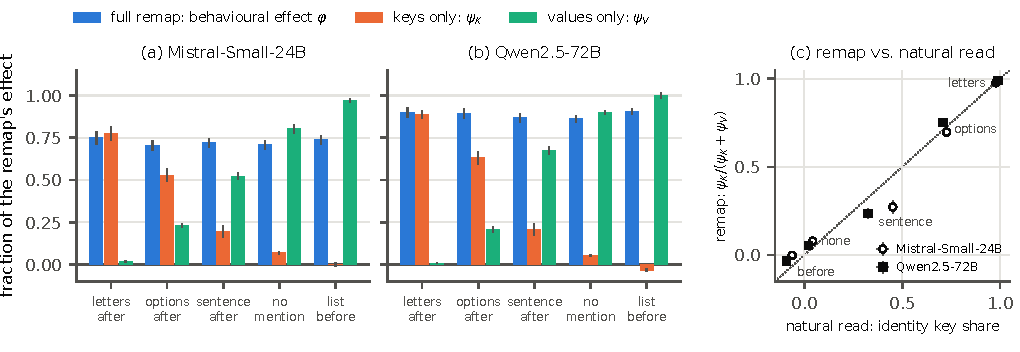
\includegraphics[width=\textwidth]{figures/fig_frames.pdf}
  \caption{\textbf{The same learned intervention has nearly the same behavioural effect in every format, but whether the writing token's keys or values carry it depends on the later mentions} (discovery sample). The released remap M of \citet{anonymous2026fitted} against the PCA patch P at Mistral-Small-24B (a) and Qwen2.5-72B (b): $\varphi$, $\psi_K$ and $\psi_V$ (\cref{eq:phi,eq:psik,eq:psiv}), exchanged from block~6 on; $n = 96$ cores $\times$ 3 fits, 95\% bootstrap intervals. (c)~The remap's key share $\psi_K/(\psi_K+\psi_V)$ against the unpatched model's $s_{\mathrm{ID}}$ in the same format: post hoc for the released remaps, preregistered (F4) for the refits (triangles; \cref{app:refit}). Diamonds: the binding swap of \citet{prakash2025lookbacks} at Qwen2.5-14B, $\kappa$ at block $\ell^*$ against $s_{\mathrm{ID}}$ from block $\ell^*{+}1$ (H7, failed); crosses: the identity edit at block~0 against $s_{\mathrm{ID}}$ from block~1 (H11, met). Values in \cref{tab:frames,tab:refit,tab:prakash}.}
  \label{fig:frames}
\end{figure}

\paragraph{Behaviour barely changes across formats; the carrying channel flips.} We then changed only the format and added a value-only exchange. Two comparisons are confirmatory and met in both models: without a later mention M's keys carry less than half of what they carry under \fmtOpt{} (C3), and M's values carry most of the effect (E4). $\varphi$ lies between \phiOptMistral{} and \phiLetterMistral{} at Mistral-Small-24B and between \phiNoneQwen{} and \phiBeforeQwen{} at Qwen2.5-72B, and the PCA control transfers the source location in every format. Yet at Qwen2.5-72B, M's keys reproduce \psiLetterQwen{} of the M$-$P difference under \fmtLetter{} but \psiNoneQwen{} under \fmtNone{}, while M's values do the reverse (\cref{fig:frames}b). Mistral-Small-24B and the removal fractions show the same crossover. Across the ten format--model cells, the remap's key share tracks the identity key share $s_{\mathrm{ID}}$ of the unpatched model in the same format (\cref{fig:frames}c; $r = \crossR{}$): post hoc for the released remaps, preregistered for the refits (\cref{app:refit}), and failed out of sample for a binding edit (\cref{app:binding}).

\paragraph{Interpretation (post hoc, discovery sample).} In \fmtLetter{}, \fmtOpt{}, \fmtPost{} and \fmtNone{} the prompt is identical up to the end of the story, so under the causal mask M writes the same key and the same value at the writing token in all four; only their readers differ, and which channel appears to carry the edit follows them. Its value half (E4) and the refit test (F) were then preregistered and confirmed. Whether this reading extends to edits obtained independently of the released remap is the channel-ratio law of the final round, which failed (\cref{sec:claim3,app:claim3}).

\paragraph{Intervention frames.} \Cref{tab:frames} gives every frame quantity with its interval. At Qwen2.5-72B, M's keys reproduce \psiLetterQwen{} of the M$-$P difference under \fmtLetter{} and \psiOptQwen{} under \fmtOpt{}, but only \psiPostQwen{} under \fmtPost{}, \psiNoneQwen{} under \fmtNone{} and $\psiBeforeQwen$ under \fmtBefore{}, while M's values do the reverse ($\psi_V$ = \psiVLetterQwen{}, \psiVOptQwen{}, \psiVPostQwen{}, \psiVNoneQwen{}, \psiVBeforeQwen{}; exploratory except C3 and E4). The removal fractions follow the addition fractions: $\chi_K$ is large where $\psi_K$ is, and $\chi_V$ where $\psi_V$ is. Among the six candidates, M's top answer is the target T in \mTLetterMistral{}--\mTPostMistral{} of (core, fit) items at Mistral-Small-24B and \mTNoneQwen{}--\mTBeforeQwen{} at Qwen2.5-72B, depending on the format.

\begin{table}[!ht]
\centering
\caption{\textbf{The intervention of \citet{anonymous2026fitted} across formats.} $\varphi$: behavioural shift of the learned remap M relative to the PCA patch P, as a fraction of the natural source-to-target shift (\cref{eq:phi}). $\psi_K$, $\psi_V$: fraction of the M$-$P difference that P reproduces when given M's keys or values at the writing token (\cref{eq:psik,eq:psiv}). $\chi_K$, $\chi_V$: fraction of that difference that M loses when given P's keys or values (\cref{app:impl}). Exchanges from block~6 on. $n = 96$ story cores with B, S and T distinct, three fits averaged within each core; 95\% bootstrap CIs over cores. Preregistrations C (C1--C3) and E (E4) for the cells they name; the rest exploratory.}
\label{tab:frames}
\resizebox{\textwidth}{!}{\begin{tabular}{llccccc}
\toprule
Model & Format & $\varphi$ & $\psi_K$ & $\chi_K$ & $\psi_V$ & $\chi_V$ \\
\midrule
Mistral-Small-24B & \fmtLetter{} & 0.75 [0.71, 0.79] & 0.78 [0.73, 0.82] & 0.99 [0.98, 0.99] & 0.02 [0.01, 0.02] & 0.16 [0.13, 0.19] \\
 & \fmtOpt{} & 0.70 [0.68, 0.73] & 0.53 [0.49, 0.57] & 0.76 [0.75, 0.78] & 0.23 [0.22, 0.24] & 0.44 [0.41, 0.48] \\
 & \fmtPost{} & 0.72 [0.69, 0.75] & 0.20 [0.16, 0.23] & 0.45 [0.43, 0.47] & 0.52 [0.50, 0.54] & 0.77 [0.73, 0.81] \\
 & \fmtNone{} & 0.71 [0.68, 0.73] & 0.07 [0.06, 0.08] & 0.18 [0.16, 0.20] & 0.80 [0.78, 0.83] & 0.93 [0.92, 0.94] \\
 & \fmtBefore{} & 0.74 [0.71, 0.76] & -0.00 [-0.01, 0.01] & 0.01 [-0.00, 0.02] & 0.97 [0.96, 0.98] & 0.96 [0.95, 0.98] \\
\midrule
Qwen2.5-72B & \fmtLetter{} & 0.90 [0.87, 0.93] & 0.89 [0.86, 0.91] & 0.99 [0.99, 1.00] & 0.01 [0.00, 0.01] & 0.17 [0.13, 0.20] \\
 & \fmtOpt{} & 0.89 [0.86, 0.92] & 0.63 [0.59, 0.67] & 0.79 [0.78, 0.81] & 0.21 [0.19, 0.23] & 0.44 [0.39, 0.48] \\
 & \fmtPost{} & 0.87 [0.84, 0.89] & 0.21 [0.17, 0.25] & 0.34 [0.31, 0.36] & 0.67 [0.65, 0.70] & 0.80 [0.76, 0.84] \\
 & \fmtNone{} & 0.86 [0.84, 0.88] & 0.05 [0.05, 0.06] & 0.11 [0.09, 0.12] & 0.90 [0.88, 0.91] & 0.95 [0.94, 0.96] \\
 & \fmtBefore{} & 0.91 [0.88, 0.92] & -0.03 [-0.04, -0.02] & -0.02 [-0.04, -0.01] & 1.00 [0.98, 1.01] & 1.01 [0.99, 1.02] \\
\bottomrule
\end{tabular}
}
\end{table}

\subsection{A remap fit without later mentions (preregistration F)}\label{app:refit}\label{sec:refit}

The remap edits block 4, upstream of every exchanged key and value. Preregistration F asked whether the format it was fit in, rather than its readers, decides its channel: at Mistral-Small-24B it refit the remap with the released code under \fmtNone{} (fit\_none) and, as a same-code control, under \fmtOpt{} (fit\_opt). All gates and all four predictions were met (\cref{tab:prereg-f,tab:refit}): fit\_none is carried by keys under \fmtLetter{} ($\psi_K = \psiLetterRefNone{}$) and by values under \fmtNone{} ($\psi_V = \psiVNoneRefNone{}$), transfers to lettered options ($\varphi = \phiLetterRefNone{}$), shows the control's crossover (F3), and its key share tracks the natural read ($r = \refRNone{}$; \cref{fig:frames}c). The reading format decides which channel dominates.

\paragraph{Recipe.} We ran the released training code of \citet{anonymous2026fitted} (\texttt{gpu/train.py} and \texttt{gpu/behavior\_engine.py}, unmodified) through \texttt{experiments/refit\_remap.py}. Its recipe: a rank-16 basis at the output of (1-based) block 4 over every event-span token; the pair-swap objective with a six-way conditional cross-entropy at the start of the reply (no prefill); AdamW, learning rate $10^{-3}$, batch 1, one shuffled epoch of their 1000 training pairs (2000 stories); seeds 101--103, which change only the order of the training pairs: every fit starts from the same PCA basis of source-minus-base differences (the randomised sketch differs by seed but returns the same subspace, mean squared principal cosine \refPcaSame{} across seeds), and that basis is the control P of every fit. The code also fits an identity-objective basis next to each remap (exploratory): its shift of the answer towards T, relative to P and as a fraction of the natural S$\to$T shift, is at most \refFstarMaxNone{} for fit\_none (under \fmtLetter{}) and \refFstarMaxOpt{} for fit\_opt. The training stories are disjoint from the 120 evaluation cores, but most evaluation event sentences also occur in some training story, as for the released remap.

\paragraph{What the wrapper replaces.} At import time, and recorded with hashes in each run's \texttt{FRAME.json}: the prompt function, for fit\_none only, by our \fmtNone{} prompt, which agrees token for token with the original prompt up to the end of the story in all 1000 training pairs; the release-integrity check, by one that tolerates only the release's mismatched \texttt{README.md}; and the model loader, by one with the same load arguments (BF16, sdpa, eval mode, no gradients, no cache, pad = eos, \texttt{fix\_mistral\_regex}) at the pinned revision, waiving the release's exact Python, package, device and memory pins and its model-asset receipt (the weights are identified instead by the pinned commit, which the loader checks). Under the causal mask the activations up to the end of the story are the same in both runs, so both start from the same P; the PCA bases came out bitwise identical across runs.

\paragraph{Results.} \Cref{tab:refit} gives every frame quantity for the two refits and for the released bases re-run in the same job; \cref{tab:prereg-f} gives the gates and predictions. The rest of this paragraph is exploratory. The control matches the released remap to within \refMaxDiffOpt{} in every quantity and format. Every fitted remap keeps \refCosFloorMin{}--\refCosFloorMax{} of its subspace (mean squared principal cosine) in the shared PCA start, against \refCosChance{} for random subspaces, so overlaps between fits lie above that floor: fit\_opt overlaps the released remap at \refCosOptMin{}--\refCosOptMax{}, while fit\_none overlaps the released remap at \refCosNoneMin{}--\refCosNoneMax{} and fit\_opt at \refCosNoneOptMin{}--\refCosNoneOptMax{}, less than two seeds of one fit overlap each other (\refCosSeedMin{}--\refCosSeedMax{}). Without the ``Answer:'' prefill, which matches the interface the remaps were fit at, the difference in differences is $\refDNoPre{}$ [$\refDNoPreLo{}$, $\refDNoPreHi{}$]. The training loss of the remap fits fell from \refLossFirstMin{}--\refLossFirstMax{} nats over the first 100 updates to \refLossLastMin{}--\refLossLastMax{} over the last 100; it starts above chance ($\ln 6 \approx 1.79$) because the PCA start transfers the source, which the pair-swap objective scores as wrong.

\paragraph{Where the fitting format still matters (post hoc).} The fitting format shifts the balance where both channels read, in the direction the stated alternative predicts. fit\_none's $\psi_K$ is lower than the control's by \refDiffOpt{} [\refDiffLoOpt{}, \refDiffHiOpt{}] under \fmtOpt{} and by \refDiffPost{} [\refDiffLoPost{}, \refDiffHiPost{}] under \fmtPost{}. It transfers better under \fmtNone{} ($\varphi = \phiNoneRefNone{}$ against \phiNoneRefOpt{}) and worse under \fmtLetter{} (\phiLetterRefNone{} against \phiLetterRefOpt{}), where its values carry almost nothing ($\psi_V = \psiVLetterRefNone{}$). These comparisons were made after seeing the data; the preregistered all-or-none alternative (\cref{tab:prereg-f}) was not observed.

\begin{table}[!ht]
\centering
\footnotesize
\caption{\textbf{Refit remaps in the frames of \citet{anonymous2026fitted}} (Mistral-Small-24B, ``Answer:'' prefill). fit\_none: refit under \fmtNone{}; fit\_opt: refit under \fmtOpt{} with the same code; released: the released bases, re-run in the same job. All fits share one PCA control P. $n = 96$ cores, three fits averaged within core; 95\% core bootstrap.}
\label{tab:refit}
{\setlength{\tabcolsep}{4pt}\begin{tabular}{llccccc}
\toprule
Remap & Format & $\varphi$ & $\psi_K$ & $\chi_K$ & $\psi_V$ & $\chi_V$ \\
\midrule
fit\_none & \fmtLetter{} & 0.67 [0.64, 0.70] & 0.77 [0.73, 0.80] & 0.98 [0.97, 0.98] & 0.02 [0.02, 0.03] & 0.15 [0.13, 0.19] \\
 & \fmtOpt{} & 0.72 [0.70, 0.74] & 0.43 [0.39, 0.47] & 0.74 [0.73, 0.76] & 0.25 [0.23, 0.26] & 0.54 [0.50, 0.58] \\
 & \fmtPost{} & 0.81 [0.79, 0.83] & 0.12 [0.10, 0.15] & 0.47 [0.44, 0.49] & 0.50 [0.47, 0.52] & 0.85 [0.81, 0.88] \\
 & \fmtNone{} & 0.81 [0.79, 0.84] & 0.07 [0.06, 0.08] & 0.18 [0.16, 0.20] & 0.80 [0.77, 0.82] & 0.93 [0.91, 0.94] \\
 & \fmtBefore{} & 0.76 [0.74, 0.78] & 0.01 [0.00, 0.02] & 0.00 [$-$0.01, 0.01] & 0.97 [0.96, 0.99] & 0.95 [0.94, 0.96] \\
\midrule
fit\_opt & \fmtLetter{} & 0.77 [0.74, 0.80] & 0.78 [0.73, 0.82] & 0.98 [0.98, 0.99] & 0.02 [0.01, 0.02] & 0.16 [0.13, 0.19] \\
 & \fmtOpt{} & 0.72 [0.69, 0.74] & 0.52 [0.48, 0.56] & 0.76 [0.74, 0.77] & 0.23 [0.22, 0.24] & 0.44 [0.40, 0.48] \\
 & \fmtPost{} & 0.73 [0.71, 0.75] & 0.20 [0.16, 0.23] & 0.45 [0.43, 0.47] & 0.52 [0.50, 0.54] & 0.77 [0.73, 0.81] \\
 & \fmtNone{} & 0.72 [0.69, 0.74] & 0.07 [0.06, 0.08] & 0.17 [0.15, 0.19] & 0.81 [0.78, 0.83] & 0.93 [0.92, 0.94] \\
 & \fmtBefore{} & 0.77 [0.74, 0.79] & 0.00 [$-$0.01, 0.01] & 0.00 [$-$0.01, 0.02] & 0.98 [0.96, 0.99] & 0.96 [0.95, 0.98] \\
\midrule
released & \fmtLetter{} & 0.75 [0.71, 0.79] & 0.78 [0.74, 0.82] & 0.99 [0.98, 0.99] & 0.02 [0.01, 0.02] & 0.16 [0.13, 0.19] \\
 & \fmtOpt{} & 0.70 [0.68, 0.73] & 0.53 [0.49, 0.57] & 0.76 [0.75, 0.78] & 0.23 [0.22, 0.24] & 0.44 [0.41, 0.48] \\
 & \fmtPost{} & 0.72 [0.69, 0.75] & 0.20 [0.16, 0.23] & 0.45 [0.43, 0.47] & 0.52 [0.50, 0.54] & 0.77 [0.73, 0.81] \\
 & \fmtNone{} & 0.71 [0.68, 0.73] & 0.07 [0.06, 0.08] & 0.18 [0.16, 0.20] & 0.80 [0.78, 0.83] & 0.93 [0.92, 0.94] \\
 & \fmtBefore{} & 0.74 [0.71, 0.76] & 0.00 [$-$0.01, 0.01] & 0.01 [0.00, 0.02] & 0.97 [0.96, 0.98] & 0.96 [0.95, 0.98] \\
\bottomrule
\end{tabular}
}
\end{table}

\subsection{The reader heads at 24B under the remap (preregistration I)}\label{app:stage7}\label{sec:link}

Preregistration I (GPU stage 7; \cref{tab:prereg-i}) was written because the two halves of the paper were linked only by inference: the reader heads were shown at two 7B models (\cref{app:heads}), the format dependence of the remap at 24B and 72B (\cref{app:remap-crossover}). It tests the link at Mistral-Small-24B on the 96 cores and released bases of the frames (\cref{tab:frames}), with M and its PCA control P patched at block 4 and the key or value of the writing token exchanged from block 6, as there.

\paragraph{The readers at 24B (Gate I-G2).} Heads are ranked by $a_3$ (\cref{app:heads}) on 60 ranking stories that share no story with the 96 cores, separately for each format, with the natural key clamped at the writing token from block~6, where the exchange starts; heads in blocks 1--5 cannot see the exchanged key and are not eligible (1120 of the 1280 heads remain). $H^*$ is the top \Ikstar{}, 5\% of all heads. On the 96 cores the option rows carry \IgtwoRatioOpt{}, \IgtwoRatioLetter{} and \IgtwoRatioPost{} of the natural key effect under \fmtOpt{}, \fmtLetter{} and \fmtPost{}. $H^*$ alone recovers $R(64)$ = \IgtwoROpt{}, \IgtwoRLetter{} and \IgtwoRPost{} of the option rows' read, and blinding $H^*$ removes $\mathrm{KO}(64)$ = \IgtwoKOOpt{}, \IgtwoKOLetter{} and \IgtwoKOPost{}; random sets of 64 recover at most \IgtwoRrandPost{} and remove at most \IgtwoKOrandPost{} (means of three). $R(64)$ is lower than at 7B only on a story type the ranking stories lack, the \InDist{} of the 96 cores whose distractor location equals B or S: on the other cores $R(64)$ = \IrSixtyfourRestOpt{}, \IrSixtyfourRestLetter{} and \IrSixtyfourRestPost{}, on those \IrSixtyfourDistOpt{}, \IrSixtyfourDistLetter{} and \IrSixtyfourDistPost{} (exploratory, recomputed, exploratory). Also exploratory: the sets of \fmtOpt{} and \fmtLetter{} share \IxOverlapOptLetter{} of 64 heads, those of \fmtOpt{} and \fmtPost{} \IxOverlapOptPost{}; ranking heads on the remap itself (P against P with M's key, in-sample on the 96 cores) gives sets that share \IremOverlapOpt{}, \IremOverlapLetter{} and \IremOverlapPost{} heads with $H^*$.

\paragraph{The remap's key read (I1--I3).} In the exchange-blinding operation, chosen heads at the option rows see P's own key at the writing token instead of M's, pinned from block 6, while every other head and row sees M's key. Blinding every head at the option rows removes $g_K$ = \IoneGOpt{} and \IoneGLetter{} of M's key-only effect (\IoneGPost{} under \fmtPost{}, reported). Blinding only $H^*$ removes \ItwoKOOpt{} and \ItwoKOLetter{} of that read (\ItwoKOPost{}), and random or active-at-$G$ sets at most \IthreeMax{}. Little of M's key effect is read outside the option rows: the key route of about one nat seen without a later mention does not persist when the candidates are mentioned, which is why some ratios against \fmtNone{} exceed 1 (\cref{app:prereg}).

\paragraph{Ablation and knockout (I4--I7).} \Cref{tab:link} gives every condition. The ablation A replaces each head's output at the option rows by its mean over the ranking stories, in every row of the frames batch, as in H3; A$^+$ adds the 32 heads of block 5; the knockout N stops the heads from attending from the option rows to the writing token. Under \fmtOpt{}, A($H^*$) removes nearly all of M's key-only effect, moves its key share near its \fmtNone{} level (I4) and raises its value-only effect by \IfiveDV{} nats, \IfiveRatio{} of the lost key effect (I5). The non-additive part of M's effect ($D - K - V$, which also holds reads of the other patched span tokens and, in block 5, of the writing token) falls from \InonAddU{} to \InonAddA{} nats (exploratory, recomputed), and $t$ = \IsixT{}. Post hoc, most of the fall in $D = m(\mathrm{M}) - m(\mathrm{P})$ is in P's rows: ablating the readers compresses every margin, so $m(\mathrm{P})$ rises from $\ImPU$ to $\ImPA$ nats while $m(\mathrm{M})$ falls only from \ImMU{} to \ImMA{}, and the unedited model's margin for its own answer over S falls from \IbMarginU{} to \IbMarginA{} nats while that answer stays the top one in every core. Under \fmtLetter{} (reported two-sided) the remap and the natural task both lose: $t$ = \IsixTLetter{}, M's target is the top answer in \IsixMTALetter{} of cases (\IsixMTLetter{} unblocked) and the natural answer in \IsixBBALetter{} of cores, consistent with the entry's caution that a lettered answer may need the readers. Under \fmtPost{} every threshold is met ($t$ = \IsixTPost{}; reported). The knockout N($H^*$) keeps more of M's effect than the ablation under \fmtOpt{} ($t$ = \InTOpt{}), and less under \fmtLetter{} ($t$ = \InTLetter{}), where answers move to the initial location in about a fifth of cases, as with the all-heads knockout at Qwen2.5-7B (G7).

\begin{table}[!ht]
\centering
\footnotesize
\caption{\textbf{The remap under each blocking at Mistral-Small-24B} (preregistration I; values as printed by the scorer). $t = D^O/D^\emptyset$; superscripts $O$ and $\emptyset$: with and without the blocking; $\kappa = K/(K+V)$ with the $\kappa$ rule (--: $\kappa$ undefined in 99\% of resamples; $\Delta_V$ not applicable or M$\to$T not printed); $\tilde\psi_K = K^O/D^\emptyset$ and $\tilde\psi_V = V^O/D^\emptyset$; $\Delta_V = V^O - V^\emptyset$, paired by core; $D$, $K$, $V$: M's effect, its key-only and its value-only part, in nats; M$\to$T: share of (core, fit) items whose top answer is M's target. A: mean-ablation of the heads' outputs at the option rows; A$^+$: with block 5; N: no attention from the option rows to the writing token. $^\dagger$Exploratory: N(all at $G$), every head at the option rows $G$; A(block 5), the 32 heads of block 5 alone; N(rand0), the first random set of 64; A($H^*_{\text{\fmtOpt{}}}$), the \fmtOpt{} set ablated under \fmtLetter{}. 95\% core-bootstrap CIs.}
\label{tab:link}
{\scriptsize\setlength{\tabcolsep}{3pt}\begin{tabular}{@{}llccccccc@{}}
\toprule
Format & Condition & $t$ & $\kappa$ & $\tilde\psi_K$ & $\tilde\psi_V$ & $\Delta_V$ (nats) & $D$ / $K$ / $V$ (nats) & M$\to$T \\
\midrule
\fmtOpt{} & unblocked & 1 & 0.698 & 0.528 & 0.229 & -- & 13.67 / 7.22 / 3.13 & 0.82 \\
 & A($H^*$) & 0.565 [0.542, 0.589] & 0.113 [0.080, 0.143] & 0.052 & 0.404 & $+$2.388 [2.141, 2.631] & 7.73 / 0.70 / 5.52 & 0.80 \\
 & A$^+$($H^*$) & 0.556 [0.534, 0.578] & 0.100 [0.067, 0.129] & 0.046 & 0.411 & $+$2.496 [2.250, 2.737] & 7.60 / 0.62 / 5.63 & 0.79 \\
 & N($H^*$) & 0.722 [0.697, 0.748] & 0.070 [0.042, 0.097] & 0.046 & 0.605 & $+$5.140 [4.835, 5.452] & 9.87 / 0.62 / 8.27 & 0.83 \\
 & N(all at $G$)$^\dagger$ & 0.739 [0.713, 0.767] & $-$0.009 & $-$0.006 & 0.684 & $+$6.220 [5.899, 6.541] & 10.11 / $-$0.08 / 9.35 & -- \\
 & A(block 5)$^\dagger$ & 1.006 [1.002, 1.010] & 0.709 & 0.561 & 0.230 & $+$0.013 [$-$0.020, 0.048] & 13.76 / 7.67 / 3.14 & -- \\
 & N(rand0)$^\dagger$ & 0.985 [0.977, 0.992] & 0.684 & 0.497 & 0.230 & $+$0.011 [$-$0.006, 0.029] & 13.47 / 6.79 / 3.14 & -- \\
\midrule
\fmtLetter{} & unblocked & 1 & 0.977 & 0.777 & 0.018 & -- & 12.87 / 9.99 / 0.23 & 0.76 \\
 & A($H^*$) & 0.385 [0.358, 0.410] & 0.661 [0.615, 0.708] & 0.179 & 0.092 & $+$0.945 [0.791, 1.102] & 4.95 / 2.30 / 1.18 & 0.46 \\
 & A$^+$($H^*$) & 0.373 [0.347, 0.398] & 0.666 [0.627, 0.706] & 0.205 & 0.102 & $+$1.086 [0.927, 1.244] & 4.80 / 2.63 / 1.32 & 0.47 \\
 & N($H^*$) & 0.296 [0.252, 0.342] & 0.466 [0.427, 0.507] & 0.134 & 0.154 & $+$1.746 [1.408, 2.122] & 3.81 / 1.73 / 1.98 & 0.39 \\
 & N(all at $G$)$^\dagger$ & 0.190 [0.156, 0.224] & -- & 0.040 & 0.137 & $+$1.524 [1.180, 1.896] & 2.44 / 0.51 / 1.76 & -- \\
 & A(block 5)$^\dagger$ & 1.017 [1.011, 1.023] & 0.976 & 0.849 & 0.021 & $+$0.038 [0.020, 0.058] & 13.09 / 10.92 / 0.27 & -- \\
 & N(rand0)$^\dagger$ & 0.978 [0.967, 0.988] & 0.977 & 0.748 & 0.018 & $-$0.007 [$-$0.027, 0.011] & 12.59 / 9.62 / 0.23 & -- \\
 & A($H^*_{\text{\fmtOpt{}}}$)$^\dagger$ & 0.373 [0.347, 0.398] & 0.646 & 0.170 & 0.093 & $+$0.961 [0.797, 1.129] & 4.80 / 2.18 / 1.19 & -- \\
\midrule
\fmtPost{} & unblocked & 1 & 0.274 & 0.196 & 0.522 & -- & 12.16 / 2.39 / 6.35 & 0.87 \\
 & A($H^*$) & 0.944 [0.928, 0.960] & 0.012 [0.000, 0.025] & 0.011 & 0.869 & $+$4.220 [3.816, 4.622] & 11.48 / 0.13 / 10.57 & 0.88 \\
 & A$^+$($H^*$) & 0.943 [0.927, 0.959] & 0.011 [$-$0.001, 0.024] & 0.010 & 0.871 & $+$4.242 [3.833, 4.650] & 11.47 / 0.12 / 10.59 & 0.88 \\
 & N($H^*$) & 0.968 [0.956, 0.982] & 0.019 [0.007, 0.031] & 0.017 & 0.910 & $+$4.722 [4.430, 5.020] & 11.78 / 0.21 / 11.07 & 0.88 \\
 & N(all at $G$)$^\dagger$ & 0.949 [0.934, 0.964] & 0.024 & 0.022 & 0.888 & $+$4.459 [4.114, 4.807] & 11.54 / 0.27 / 10.81 & -- \\
 & A(block 5)$^\dagger$ & 1.005 [1.003, 1.007] & 0.294 & 0.214 & 0.516 & $-$0.075 [$-$0.113, $-$0.033] & 12.23 / 2.61 / 6.27 & -- \\
 & N(rand0)$^\dagger$ & 0.998 [0.996, 1.000] & 0.250 & 0.180 & 0.540 & $+$0.220 [0.144, 0.306] & 12.14 / 2.19 / 6.57 & -- \\
\bottomrule
\end{tabular}
}
\end{table}

\paragraph{Summary.} The remap's key-only effect at Mistral-Small-24B is read at the option words and through the natural reader heads, not through random or active sets (I1--I3); ablating these heads moves its key share under \fmtOpt{} near the \fmtNone{} level (I4) and raises what its values carry (I5), but keeps only part of its effect on the margin (I6, not met; the entry's partial takeover), and Gate I-G4, which reading the kept part as a value takeover requires, failed. Qwen2.5-72B was not run.

\subsection{The frames under the emitted-form score (final round)}\label{app:remap-emitted}

The discovery sample scored the frames on the lower-case candidate tokens. In the final round the frames at Mistral-Small-24B were re-measured on the 96 native cores of the release with the released bases, scored both ways in the same pass, the emitted-form score using the model's own frames (risky measurement-validity line J-B8, met). All twelve differences between the two scores (of $\varphi$, $\psi_K$ and $\psi_V$, under \fmtOpt{}, \fmtNone{}, \fmtBefore{} and \fmtPost{}) have 95\,\% paired core-bootstrap intervals within [\JbEightLoMin{}, \JbEightHiMax{}], inside the preregistered $\pm 0.05$, and the emitted forms carry \JbEightMEMin{}--\JbEightMEMax{} of the natural run's probability mass. For example, without a later mention $\psi_V$ is \JbEightPsiVLNone{} under the lower-case score and \JbEightPsiVENone{} under emitted forms, and under \fmtOpt{} $\psi_K$ is \JbEightPsiKLOpt{} and \JbEightPsiKEOpt{}. The crossover is therefore not an artefact of the lower-case score.

\clearpage
% Appendix H: the binding swap of Prakash et al. Input by sections/appendix.tex.
\section{The binding swap of Prakash et al.}\label{app:binding}\label{sec:prakash}

Preregistration H applied the key-only and value-only exchange to an edit we did not design: the state-token patch BIND of \citet{prakash2025lookbacks}, at Qwen2.5-14B on their material, with an identity edit ID as a control. Its four predictions on the swap (H7--H10) failed. The final round asked two narrower questions on the same material: whether an identity edit is copy-read at the swap's depth (J-C6), and whether any model has a depth at which the binding swap works while the identity key route is still open, the only depth at which the two kinds of edit could be compared (the overlap screen). \Cref{tab:prereg-h} gives the verdicts of H, and \cref{app:prereg-j} those of the final round.

\subsection{The exchange at Qwen2.5-14B (preregistration H, part (b))}\label{app:prakash}

BIND replicates (IIA \PkGatebOneBind{} at block \PkLstar{} under \fmtNone{}; Gate b1).

\paragraph{The binding swap is key-dominant; four predictions failed.}
Without a later mention, keys carry most of BIND's effect and values a substantial share ($\psi_K = \PkPsiKBindNone{}$, $\psi_V = \PkPsiVBindNone{}$, $\kappa = \PkKappaBindNone{}$). Under \textsc{qnames} and \fmtOpt{}, $\kappa = \PkKappaBindQnames{}$ and \PkKappaBindOpt{}, but BIND flips \PkNflipBindQnames{}/\PkN{} answers there (exploratory count), so these decompose a shift of the logit margin; \fmtLetter{} failed the effect-size gate. Not met: values carrying BIND without a later mention (H8); a crossover of at least 0.4 (later mentions raised $\kappa$ by \HnineDiff{} [\HnineDiffLo{}, \HnineDiffHi{}], and \textsc{qnames} is not in between; H9); the rival $\kappa \leq 0.25$ (H10; nor is $\kappa \geq 0.75$ throughout); and the law $\kappa \approx s_{\mathrm{ID}}$, which missed by \HsevenGapMin{}--\HsevenGapMax{} (H7; \cref{fig:frames}c).

\paragraph{The identity edit, and depth.}
ID at block 0 matched the law ($\kappa_{\mathrm{ID}}$ = \PkKappaIdZeroNone{}, \PkKappaIdZeroQnames{}, \PkKappaIdZeroOpt{} against $s_{\mathrm{ID}}$ = \HelevenSidNone{}, \HelevenSidQnames{}, \HelevenSidOpt{}), and later mentions raised $\kappa_{\mathrm{ID}}$ by \HelevenDiff{} [\HelevenDiffLo{}, \HelevenDiffHi{}] (H11, met). This is consistency on their material, not out-of-sample support: at block 0 ID nearly equals the natural clamp, and H11's block-28 part compares values near zero. Post hoc, at block 28 BIND is key-dominant while ID is value-carried ($\psi_V \geq \PkPsiVIdTwentyeightOpt{}$ in the evaluable formats), which is consistent with the H7 failure but does not explain it. Depth is an alternative explanation (below): no depth has both the binding swap and a key-read identity route, so whether the kind of edit or its depth sets how far the format moves the attribution is untested.

\paragraph{Material and population.} We use the template-2 stories of \citet{prakash2025lookbacks}, their raw prompt (an instruction, the story, ``Question:'' and ``Answer:'', without a chat template) and their pool of \PkNpool{} reversed-sentence pairs drawn with their seed. In each story two characters each fill an opaque bottle with a drink, in two sentences, and the question asks what one character believes their bottle contains. The release is fetched at run time and checked by hash, and our port reproduces their pool byte for byte. Their language-model filter under \fmtNone{} passed \PkNpass{} pairs at Qwen2.5-14B-Instruct; the population is the first \PkN{} passing pairs in pool order, of which about \PkOverlap{} are in their 80-pair validation split. The formats differ only after the story: \fmtNone{} is their question; \textsc{qnames} names four candidate drinks in the question (the two story drinks and two drinks S and X absent from the story); \fmtOpt{} lists the same four as choices with ``Answer with exactly one choice''; \fmtLetter{} letters them (exploratory); and \textsc{qnames2} (exploratory) names only the two story drinks, as the questions of their preliminary second dataset do.

\paragraph{The two edits.} BIND is their state-token patch: at the output of block $\ell^*$, the residuals at the two drink words and the punctuation after each are set to those of the counterfactual in which the two sentences are exchanged, each position taking the other sentence's. The drink words' identity does not change; their ordering information does. These are the ordering IDs on which the binding, answer and visibility lookbacks of \citet{prakash2025lookbacks} are built, so the swap is not an identity edit. ID substitutes, at block $\ell^*_{\mathrm{ID}}$, the queried drink's span from a donor story in which that drink is replaced by S. With $m = \log p(\text{target}) - \log p(\text{queried drink})$, where the target is the other story drink for BIND and S for ID, IIA is the fraction of pairs whose patched answer is the target, and $\ell^*$ and $\ell^*_{\mathrm{ID}}$ are the earliest blocks whose IIA under \fmtNone{} is within 0.01 of the maximum.

\begin{table}[!ht]
\centering
\small
\caption{\textbf{Replication of the binding swap} (Qwen2.5-14B-Instruct, \fmtNone{}, IIA of BIND by patched block). Released: the per-layer values published with \citet{prakash2025lookbacks} on their 80 validation pairs, transcribed from their release (not part of our results). Ours: \PkN{} pairs, and the \PkSharedN{} pairs shared with their validation split (exploratory). Recomputed from our sweep files; a reproduction check, since the released values were seen before preregistration H was finalised.}
\label{tab:replication}
\begin{tabular}{@{}lccc@{}}
\toprule
Block & Prakash et al.\ (80 pairs) & ours (150 pairs) & ours, 70 shared pairs \\
\midrule
24 & 0.69 & 0.720 & 0.700 \\
26 & 0.72 & 0.747 & 0.729 \\
28 & 1.00 & 0.993 & 1.000 \\
30--34 & 1.00 & 1.000 & 1.000 \\
36 & 0.06 & 0.080 & 0.057 \\
\bottomrule
\end{tabular}

\end{table}

\paragraph{Replication and sweeps.} The swap reproduces their released per-layer IIA (\cref{tab:replication}). Its IIA is 1.00 at blocks 29--34 and \PkGatebOneBind{} at 28, where one pair fails; the tie rule selects $\ell^* = \PkLstar{}$, and one more failure would have selected 29. Below block 24 it flips no answer under \fmtNone{} (IIA \PkSweepIIABindNoneTwentythree{} at block 23, \PkSweepIIABindNoneTwentyfour{} at 24). \Cref{fig:sweeps} shows every sweep. The swap reproduces only under \fmtNone{}: under \textsc{qnames}, \fmtOpt{} and \fmtLetter{} its IIA is at most \PkSweepIIABindQnamesTwentythree{} at every swept block from 18 to 40, and its effect on the margin peaks at \PkSweepPhiBindOptTwentyeight{} nats (\fmtOpt{}, block 28), \PkSweepPhiBindQnamesThirtyone{} (\textsc{qnames}, block 31) and \PkSweepPhiBindLetterTwentythree{} (\fmtLetter{}, block 23). The identity edit flips every answer under \fmtNone{} at every block through 35, so its curve is flat and the tie rule picks $\ell^*_{\mathrm{ID}} = \PkLstarId{}$ by default rather than by localisation. When the candidates are named after the question it stops flipping answers from about block 20: under \fmtOpt{} its IIA is \PkSweepIIAIdOptEleven{} through block 11, \PkSweepIIAIdOptFourteen{} at 14, \PkSweepIIAIdOptSixteen{} at 16, \PkSweepIIAIdOptNineteen{} at 19 and \PkSweepIIAIdOptTwenty{} from 20; under \textsc{qnames} it is \PkSweepIIAIdQnamesZero{} at block 0 and \PkSweepIIAIdQnamesTwenty{} from 20.

\begin{figure}[!ht]
\centering
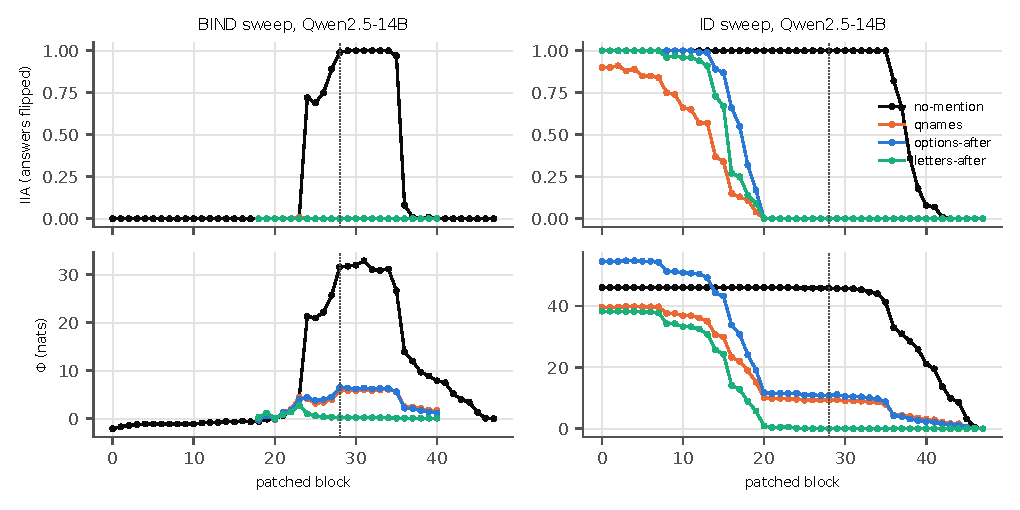
\includegraphics[width=\textwidth]{figures/fig_sweeps.pdf}
\caption{\textbf{Sweeps of the two edits over the patched block} (Qwen2.5-14B-Instruct, \PkN{} pairs, BF16). Top: IIA, the fraction of answers flipped to the target; bottom: $\Phi$, the mean shift of $m = \log p(\text{target}) - \log p(\text{queried drink})$. Left: the binding swap BIND (swept over blocks 18--40 in the formats that name candidates); right: the identity edit ID. Dotted: block $\ell^* = \PkLstar{}$. $\ell^*$ and $\ell^*_{\mathrm{ID}}$ are chosen on the \fmtNone{} sweeps (preregistered); the other formats are reported.}
\label{fig:sweeps}
\end{figure}

\paragraph{The exchange.} The exchange (\cref{app:impl}) exchanges the patched positions' keys or values in every block after the patched one. A cell is evaluable if Gates b0 and b2 pass in it ($\Phi \geq 3$ nats), $\psi_K + \psi_V \geq 0.5$ with both at least $-0.1$, and the edit reproduces at that depth on the \fmtNone{} sweep. \Cref{tab:prakash} summarises the cells and \cref{tab:exchange} gives all thirteen. \fmtLetter{} fails Gate b2 at block 28 for both edits ($\Phi$ = \PkPhiBindLetter{} and \PkPhiIdTwentyeightLetter{} nats), and ID@28 under \fmtLetter{} also fails the $\kappa$ rule; \fmtLetter{} is exploratory throughout. BIND reproduces fully under \fmtNone{} (it flips \PkNflipBindNone{} of \PkN{} answers; exploratory count), and that cell carries H8 by itself. Under \textsc{qnames} and \fmtOpt{} it flips \PkNflipBindQnames{} and \PkNflipBindOpt{} answers, so those cells decompose a shift of the logit margin ($\Phi$ = \PkPhiBindQnames{} and \PkPhiBindOpt{} nats against base margins of $\PkMarginBindQnames$ and $\PkMarginBindOpt$, exploratory, recomputed), not a reproduced swap.

\begin{table}[!ht]
\centering
\caption{\textbf{The exchange on the interventions of \citet{prakash2025lookbacks}} (Qwen2.5-14B-Instruct, \PkN{} pairs). Each cell: $\kappa = \psi_K/(\psi_K+\psi_V)$ with ($\psi_K$, $\psi_V$), the number of answers the full patch flips, and its effect $\Phi$ on the margin (nats). BIND@28: the binding swap at block $\ell^* = \PkLstar{}$; ID@0, ID@28: the identity edit at blocks 0 and 28. $s_{\mathrm{ID}}(f, \ell_0)$: identity key share of the natural clamp at the queried drink from block $\ell_0$, with 95\% CI. $^\dagger$Exploratory formats. $^\ddagger$Gate b2 failed ($\Phi < 3$ nats). n/e: the $\kappa$ rule fails. H7 compares BIND@28 with $s_{\mathrm{ID}}(f, 29)$, H11 ID@0 with $s_{\mathrm{ID}}(f, 1)$ (Part 1) and ID@28 with $s_{\mathrm{ID}}(f, 29)$ (Part 2).}
\label{tab:prakash}
\resizebox{\textwidth}{!}{\begin{tabular}{@{}lccccc@{}}
\toprule
 & \fmtNone{} & \textsc{qnames} & \fmtOpt{} & \fmtLetter{}$^\dagger$ & \textsc{qnames2}$^\dagger$ \\
\midrule
BIND@28 & \begin{tabular}[t]{@{}c@{}}$\kappa$ 0.618 (0.703, 0.435)\\[-1pt]{\scriptsize flips 149/150, $\Phi$ 31.616}\end{tabular} & \begin{tabular}[t]{@{}c@{}}$\kappa$ 0.906 (1.020, 0.106)\\[-1pt]{\scriptsize flips 0/150, $\Phi$ 5.814}\end{tabular} & \begin{tabular}[t]{@{}c@{}}$\kappa$ 0.864 (1.025, 0.161)\\[-1pt]{\scriptsize flips 0/150, $\Phi$ 6.523}\end{tabular} & \begin{tabular}[t]{@{}c@{}}$\kappa$ 0.658 (1.652, 0.859)\\[-1pt]{\scriptsize flips 0/150, $\Phi$ 0.225$^\ddagger$}\end{tabular} & \begin{tabular}[t]{@{}c@{}}$\kappa$ 1.014 (1.016, $-$0.014)\\[-1pt]{\scriptsize flips 0/150, $\Phi$ 7.285}\end{tabular} \\
ID@0 & \begin{tabular}[t]{@{}c@{}}$\kappa$ 0.131 (0.131, 0.871)\\[-1pt]{\scriptsize flips 150/150, $\Phi$ 46.005}\end{tabular} & \begin{tabular}[t]{@{}c@{}}$\kappa$ 0.773 (0.777, 0.229)\\[-1pt]{\scriptsize flips 135/150, $\Phi$ 39.606}\end{tabular} & \begin{tabular}[t]{@{}c@{}}$\kappa$ 0.779 (0.789, 0.224)\\[-1pt]{\scriptsize flips 150/150, $\Phi$ 54.550}\end{tabular} & \begin{tabular}[t]{@{}c@{}}$\kappa$ 0.969 (0.977, 0.031)\\[-1pt]{\scriptsize flips 150/150, $\Phi$ 38.255}\end{tabular} & -- \\
ID@28 & \begin{tabular}[t]{@{}c@{}}$\kappa$ 0.129 (0.129, 0.872)\\[-1pt]{\scriptsize flips 150/150, $\Phi$ 45.797}\end{tabular} & \begin{tabular}[t]{@{}c@{}}$\kappa$ 0.007 (0.006, 0.827)\\[-1pt]{\scriptsize flips 0/150, $\Phi$ 9.321}\end{tabular} & \begin{tabular}[t]{@{}c@{}}$\kappa$ 0.006 (0.005, 0.811)\\[-1pt]{\scriptsize flips 0/150, $\Phi$ 10.885}\end{tabular} & \begin{tabular}[t]{@{}c@{}}n/e ($-$0.171, 3.024)\\[-1pt]{\scriptsize flips 0/150, $\Phi$ 0.034$^\ddagger$}\end{tabular} & -- \\
\midrule
$s_{\mathrm{ID}}(f, 29)$ & \begin{tabular}[t]{@{}c@{}}0.017\\[-1pt]{\scriptsize [0.007, 0.026]}\end{tabular} & \begin{tabular}[t]{@{}c@{}}$-$0.028\\[-1pt]{\scriptsize [$-$0.039, $-$0.019]}\end{tabular} & \begin{tabular}[t]{@{}c@{}}$-$0.015\\[-1pt]{\scriptsize [$-$0.020, $-$0.010]}\end{tabular} & \begin{tabular}[t]{@{}c@{}}0.098\\[-1pt]{\scriptsize [$-$2.155, 1.750]}\end{tabular} & -- \\
$s_{\mathrm{ID}}(f, 1)$ & \begin{tabular}[t]{@{}c@{}}0.017\\[-1pt]{\scriptsize [0.007, 0.026]}\end{tabular} & \begin{tabular}[t]{@{}c@{}}0.724\\[-1pt]{\scriptsize [0.710, 0.739]}\end{tabular} & \begin{tabular}[t]{@{}c@{}}0.702\\[-1pt]{\scriptsize [0.689, 0.716]}\end{tabular} & \begin{tabular}[t]{@{}c@{}}0.984\\[-1pt]{\scriptsize [0.976, 0.992]}\end{tabular} & -- \\
\bottomrule
\end{tabular}
}
\end{table}

\begin{table}[!ht]
\centering
\caption{\textbf{All thirteen exchange cells} (Qwen2.5-14B-Instruct, \PkN{} pairs). $\Phi$: effect of the full patch on $m$ (nats) with 95\% CI; flips: answers moved to the target; $\psi_K$, $\psi_V$: fractions of $\Phi$ reproduced in the clean run by the patched run's keys or values at the patched positions; interaction $1 - \psi_K - \psi_V$; $\kappa$ with 95\% CI; $\kappa_w$: $\kappa$ with the drink words alone exchanged (punctuation positions excluded); $\chi_K$, $\chi_V$: fractions of $\Phi$ lost when the patched run gets the clean keys or values. \fmtLetter{} and \textsc{qnames2} are exploratory; $\kappa_w$, $\chi_K$ and $\chi_V$ are exploratory everywhere.}
\label{tab:exchange}
\resizebox{\textwidth}{!}{\begin{tabular}{@{}llccccccccc@{}}
\toprule
Edit & Format & $\Phi$ (nats) & flips & $\psi_K$ & $\psi_V$ & interaction & $\kappa$ & $\kappa_w$ & $\chi_K$ & $\chi_V$ \\
\midrule
BIND@28 & \fmtNone{} & 31.616 [30.193, 32.985] & 149/150 & 0.703 & 0.435 & $-$0.138 & 0.618 [0.595, 0.640] & 0.779 & 0.565 & 0.297 \\
 & \textsc{qnames} & 5.814 [5.187, 6.456] & 0/150 & 1.020 & 0.106 & $-$0.127 & 0.906 [0.879, 0.931] & 0.919 & 0.894 & $-$0.020 \\
 & \fmtOpt{} & 6.523 [5.905, 7.171] & 0/150 & 1.025 & 0.161 & $-$0.186 & 0.864 [0.839, 0.889] & 0.875 & 0.839 & $-$0.025 \\
 & \fmtLetter{} & 0.225 [0.170, 0.282] & 0/150 & 1.652 & 0.859 & $-$1.511 & 0.658 [0.559, 0.854] & 0.278 & 0.141 & $-$0.652 \\
 & \textsc{qnames2} & 7.285 [6.734, 7.861] & 0/150 & 1.016 & $-$0.014 & $-$0.002 & 1.014 [0.992, 1.034] & 1.019 & 1.014 & $-$0.016 \\
\midrule
ID@0 & \fmtNone{} & 46.005 [45.276, 46.725] & 150/150 & 0.131 & 0.871 & $-$0.002 & 0.131 [0.119, 0.142] & 0.132 & 0.129 & 0.869 \\
 & \textsc{qnames} & 39.606 [38.747, 40.488] & 135/150 & 0.777 & 0.229 & $-$0.006 & 0.773 [0.759, 0.786] & 0.749 & 0.771 & 0.223 \\
 & \fmtOpt{} & 54.550 [53.652, 55.462] & 150/150 & 0.789 & 0.224 & $-$0.012 & 0.779 [0.764, 0.793] & 0.737 & 0.776 & 0.211 \\
 & \fmtLetter{} & 38.255 [37.690, 38.788] & 150/150 & 0.977 & 0.031 & $-$0.008 & 0.969 [0.960, 0.977] & 0.957 & 0.969 & 0.023 \\
\midrule
ID@28 & \fmtNone{} & 45.797 [45.069, 46.514] & 150/150 & 0.129 & 0.872 & $-$0.001 & 0.129 [0.118, 0.140] & 0.131 & 0.128 & 0.871 \\
 & \textsc{qnames} & 9.321 [8.653, 9.995] & 0/150 & 0.006 & 0.827 & 0.166 & 0.007 [$-$0.004, 0.018] & 0.009 & 0.173 & 0.994 \\
 & \fmtOpt{} & 10.885 [10.314, 11.513] & 0/150 & 0.005 & 0.811 & 0.185 & 0.006 [$-$0.003, 0.013] & 0.003 & 0.189 & 0.995 \\
 & \fmtLetter{} & 0.034 [$-$0.012, 0.078] & 0/150 & $-$0.171 & 3.024 & $-$1.854 & n/e & $-$0.263 & $-$2.024 & 1.171 \\
\bottomrule
\end{tabular}
}
\end{table}

\paragraph{Further exchange results (exploratory).} Part of BIND's value share under \fmtNone{} sits at the punctuation positions: with the drink words alone exchanged, $\psi_V$ falls from \PkPsiVBindNone{} to \PkPsiVwBindNone{} and $\kappa_w$ = \PkKappaWBindNone{} (exploratory, recomputed); under \textsc{qnames} and \fmtOpt{}, $\kappa_w$ is close to $\kappa$ (\cref{tab:exchange}). Split by the queried character, BIND under \fmtNone{} gives $\psi_K$ = \PkPsiKqZeroBindNone{} and $\psi_V$ = \PkPsiVqZeroBindNone{} for the first ($n = \PkNqZeroBindNone{}$) and \PkPsiKqOneBindNone{} and \PkPsiVqOneBindNone{} for the second ($n = \PkNqOneBindNone{}$). Under \textsc{qnames2}, which names only the two story drinks, the margin shift is carried by keys alone ($\kappa$ = \PkKappaBindQnamestwo{}, $\psi_V$ = $\PkPsiVBindQnamestwo$), but no answer flips. At block 28 the identity edit is value-carried in every evaluable format ($\psi_V$ = \PkPsiVIdTwentyeightNone{} / \PkPsiVIdTwentyeightQnames{} / \PkPsiVIdTwentyeightOpt{}), while BIND is key-dominant (\cref{tab:prakash}); this is the post hoc reading of \cref{sec:prakash}, with its caveats there: under \textsc{qnames} and \fmtOpt{} neither edit flips an answer, BIND also moves a payload, and Gate b3, built for the reverse dissociation, failed.

\begin{table}[!ht]
\centering
\caption{\textbf{Identity key share of the natural clamp on the stories of \citet{prakash2025lookbacks}} (Qwen2.5-14B-Instruct, \PkN{} pairs). $s_{\mathrm{ID}} = \overline{\mathrm{ID}}_K/(\overline{\mathrm{ID}}_K + \overline{\mathrm{ID}}_V)$ for keys and values clamped at the queried drink word from block $\ell_0$ on. The onsets 0, 1, 3, 14 and 29 are preregistered in the four formats; the others form an exploratory sweep in \fmtNone{} and \fmtOpt{}. Under \fmtLetter{} at $\ell_0 = 29$ the denominator is near zero, so $s_{\mathrm{ID}}$ is undetermined (CI in \cref{tab:prakash}).}
\label{tab:clamp}
\resizebox{\textwidth}{!}{\begin{tabular}{@{}lcccccccccccccc@{}}
\toprule
Format & $\ell_0{=}0$ & $\ell_0{=}1$ & $\ell_0{=}3$ & $\ell_0{=}6$ & $\ell_0{=}12$ & $\ell_0{=}14$ & $\ell_0{=}18$ & $\ell_0{=}24$ & $\ell_0{=}27$ & $\ell_0{=}29$ & $\ell_0{=}30$ & $\ell_0{=}33$ & $\ell_0{=}36$ & $\ell_0{=}42$ \\
\midrule
\fmtNone{} & 0.018 & 0.017 & 0.017 & 0.017 & 0.018 & 0.017 & 0.017 & 0.017 & 0.017 & 0.017 & 0.017 & 0.018 & 0.021 & 0.036 \\
\textsc{qnames} & 0.724 & 0.724 & 0.726 & -- & -- & 0.488 & -- & -- & -- & $-$0.028 & -- & -- & -- & -- \\
\fmtOpt{} & 0.702 & 0.702 & 0.702 & 0.688 & 0.634 & 0.587 & 0.218 & 0.041 & $-$0.014 & $-$0.015 & $-$0.016 & $-$0.015 & $-$0.018 & $-$0.070 \\
\fmtLetter{} & 0.984 & 0.984 & 0.984 & -- & -- & 0.975 & -- & -- & -- & 0.098 & -- & -- & -- & -- \\
\bottomrule
\end{tabular}
}
\end{table}

\paragraph{Depth.} The identity key route at the drink word closes with depth when candidates are named after the question (\cref{tab:clamp}): under \fmtOpt{}, $s_{\mathrm{ID}}$ is \PkSidOptZero{} for $\ell_0 \leq 3$, \PkSidOptFourteen{} at 14, \PkSidOptEighteen{} at 18, \PkSidOptTwentyfour{} at 24 and $\PkSidOptTwentyseven$ at 27, while under \fmtNone{} it stays near zero at every onset. Gate b3, which H10's reading as a dissociation needed, failed: at $\ell_0 = 29$ under \fmtOpt{}, $\mathrm{ID}_K$ = $\PkGatebThreeIDK$ nats and $s_{\mathrm{ID}}$ = $\PkGatebThreeSid$, and $\kappa_{\mathrm{ID}}$ at block 28 is \PkGatebThreeKappa{}. The binding swap flips no answer below block 24 under \fmtNone{} and at most \PkSweepIIABindQnamesTwentythree{} of answers at any swept block (18--40) when candidates are named, while the identity edit stops flipping answers from about block 20 when they are named, and the key route of identity has closed by block 24. No depth has both the binding swap and a key-read identity route, so the contrast between the identity edit at block 0 (a format shift of $+\HelevenDiff{}$) and the binding swap at block 28 ($+\HnineDiff{}$) is confounded with depth: whether the kind of edit or its depth decides how far the format moves the attribution is untested.

\paragraph{$\kappa$ and $s_{\mathrm{ID}}$ are different statistics.} $\kappa$ is one-sided ($m$ compares the target with the queried drink) and exchanges the drink word and the punctuation after it; $s_{\mathrm{ID}}$ is the symmetric S-against-X identity contrast at the word alone. With $\ell^*_{\mathrm{ID}} = \PkLstarId{}$, the ID@0 exchange and the natural clamp from block 1 are nearly the same intervention: applied to both, the one-sided $\kappa$ agree within \PkClampAgreeNone{} (\fmtNone{}), \PkClampAgreeQnames{} (\textsc{qnames}), \PkClampAgreeOpt{} (\fmtOpt{}) and \PkClampAgreeLetter{} (\fmtLetter{}) (exploratory, recomputed). The H11 Part 1 gaps therefore split as follows: under \fmtNone{} almost the whole gap is the difference between the statistics (\PkClampStatGapNone{}); under \textsc{qnames}, \PkClampAgreeQnames{} is exchange against clamp and \PkClampStatGapQnames{} the difference between the statistics; under \fmtOpt{}, \PkClampAgreeOpt{} and \PkClampStatGapOpt{} (exploratory, recomputed; the log's split, from three-decimal printed values, differs in the last digit). H11 Part 2, at block 28, compares values within a few hundredths of zero under \textsc{qnames} and \fmtOpt{} ($\kappa_{\mathrm{ID}}$ = \PkKappaIdTwentyeightQnames{} and \PkKappaIdTwentyeightOpt{} against $s_{\mathrm{ID}}$ = $\HsevenSidQnames$ and $\HsevenSidOpt$) and repeats Part 1's \fmtNone{} cell (\PkKappaIdTwentyeightNone{} against \HsevenSidNone{}). H11 is thus consistency of the exchange with the clamp on their material, not an independent test of the law. For H7, the one-sided clamp analogue from block 29 is \PkClampKappaNoneTwentynine{} / \PkClampKappaQnamesTwentynine{} / \PkClampKappaOptTwentynine{} (exploratory, recomputed), which would leave every gap far above 0.25; no verdict depends on the difference between the statistics. H7's correlation, $r = \HsevenR$, is computed over three values of $s_{\mathrm{ID}}$ within a few hundredths of zero and carries no information. Against $s_{\mathrm{ID}}$ from block 0 (H7's secondary comparison, not scored), the gaps are \HsevenGapZeroNone{}, \HsevenGapZeroQnames{} and \HsevenGapZeroOpt{}.

\paragraph{FP32 re-check (exploratory, recomputed).} Re-running the \fmtNone{} sweeps in FP32 at blocks 26--30 gives BIND IIA of \PkFpIIATwentysix{}, \PkFpIIATwentyseven{}, \PkFpIIATwentyeight{}, \PkFpIIATwentynine{} and \PkFpIIAThirty{}, against \PkBfIIATwentysix{}, \PkBfIIATwentyseven{}, \PkBfIIATwentyeight{}, \PkBfIIATwentynine{} and \PkBfIIAThirty{} in BF16, so the tie rule again selects block 28. At block 28 the flips agree in \PkFpAgree{} of pairs (a different single pair fails in FP32), and $\Phi$ differs by \PkFpPhiDiff{} nats. The identity edit's IIA is \PkFpIdIIAMin{} at blocks 0--2 in both precisions.

\subsection{The final round: an identity edit at block 28 and the overlap screen}\label{app:binding-j}

\paragraph{An identity edit at block 28 (J-C6, met).} The identity edit of H was the residual of a donor story, which at block 28 nearly restates the natural clamp. J-C6 replaced it by a steering vector \citep{panickssery2023caa}: the mean difference of the block-28 states at the drink word and the punctuation after it between stories with the drink S and with the queried drink, taken over the pool pairs outside the population, written at block 28 of Qwen2.5-14B. Its anchor gate reproduced H's binding swap (IIA \JcGsevenIIA{}; $\kappa_{\mathrm{BIND}}$ = \JcGsevenKappaNoMention{}, \JcGsevenKappaQnames{} and \JcGsevenKappaOptAfter{} under \fmtNone{}, \textsc{qnames} and \fmtOpt{}, equal to stage 6). The steering vector flips every answer without a later mention (IIA \JcSixFlip{}), and its keys and values lie at a relative distance $\nu$ = \JcSixNuNoMention{} from those of H's identity edit. The pre-written text, used verbatim: ``At block 28 of Qwen2.5-14B an identity edit is copy-read like the natural value ($\kappa \leq 0.30$), while the binding swap there is key-read; key-flat reading is not a property of depth for identity edits.'' Its key share is $\kappa_{\mathrm{CAA}}$ = \JcSixKappaCaaNoMention{} [\JcSixKappaCaaNoMentionLo{}, \JcSixKappaCaaNoMentionHi{}], \JcSixKappaCaaQnames{} and \JcSixKappaCaaOptAfter{} in the three formats, and $\kappa_{\mathrm{BIND}} - \kappa_{\mathrm{CAA}}$ = \JcSixDiffNoMention{} [\JcSixDiffNoMentionLo{}, \JcSixDiffNoMentionHi{}], \JcSixDiffQnames{} [\JcSixDiffQnamesLo{}, \JcSixDiffQnamesHi{}] and \JcSixDiffOptAfter{} [\JcSixDiffOptAfterLo{}, \JcSixDiffOptAfterHi{}] (95\,\% pair-bootstrap intervals). This does not separate kind from depth, because the natural read there is itself copy-only, and the swap changes no answer in two of the three formats: under \textsc{qnames} and \fmtOpt{} the binding swap's IIA is \JcSixIIABindQnames{} and \JcSixIIABindOptAfter{} (\JcSixIIABindNoMention{} under \fmtNone{}), so its $\kappa$ there describes margin shifts of \JcSixPhiBindQnames{} and \JcSixPhiBindOptAfter{} nats that change no answer. % verbatim: J-C6 text, outcome J part C

\paragraph{The overlap screen (J-C-SCREEN, met; J-C-WIN, not evaluable).} At Qwen2.5-7B and Llama-3.1-8B the binding swap was swept over every block under \fmtNone{} (150 pairs passing the language-model filter in each model), and the natural identity key share $s_{\mathrm{ID}}$ under \fmtOpt{} was measured from the block after each working block and on a grid. A window would be a block where the swap works ($\Phi \geq 3$ nats and IIA $\geq 0.5$) and $s_{\mathrm{ID}}(l{+}1) \geq 0.4$. The swap works at blocks \JcScreenWbFirstQwenSeven{}--\JcScreenWbLastQwenSeven{} of Qwen2.5-7B (IIA up to \JcScreenMaxIIAQwenSeven{}) and \JcScreenWbFirstLlamaEight{}--\JcScreenWbLastLlamaEight{} of Llama-3.1-8B (up to \JcScreenMaxIIALlamaEight{}), where $s_{\mathrm{ID}}(l{+}1)$ is at most \JcScreenSidWbMaxQwenSeven{} and \JcScreenSidWbMaxLlamaEight{}; the identity key route is open early ($s_{\mathrm{ID}}$ from block 0: \JcScreenSidZeroQwenSeven{} and \JcScreenSidZeroLlamaEight{}) and has closed before the swap begins to work. The pre-written text, with its codes as written: ``Binding forms only after the identity key route closes in every model screened, so a binding swap cannot be compared with an identity edit at a depth where the key route is open; H7--H10 stand.'' Without a window, J-C-WIN, which would have tested the law inside it, is not evaluable. % verbatim: C-12 screen text, entry J part C

\clearpage
% Appendix I: competing accounts and further related work. Input by sections/appendix.tex.
\section{Competing accounts and further related work}\label{app:accounts}\label{app:discussion}

\paragraph{What four accounts predict (as of the earlier entries).}
\Cref{tab:accounts} sets four accounts against the observations of the discovery sample. Each, ours included, is contradicted somewhere. Two rows matter most: the binding swap, where our account's preregistered extension failed (H7, H9) and the lookback account is partly compatible, post hoc (one edit, one model); and I6, where at 24B less of the remap's effect was kept than predicted once its readers were ablated.

\begin{table}[!ht]
  \centering
  \caption{\textbf{What four accounts predict, as of the entries of the discovery sample.} DT: duplicate-token attention alone; LB: lookback addresses and payloads \citep{prakash2025lookbacks,wu2026record}; FF: an edit's channel is set by the format it was fit in; LM: later-mention readers (ours). $\checkmark$: predicted and observed; $\times$: predicted otherwise (refuted); --: silent; (ph): compatible, post hoc; $\checkmark$/$\times$: the attention is predicted, its presence without a read is not; $\checkmark$/(ph): the attention is predicted, its presence without a read is explained post hoc (the read is decided downstream). Binding-swap row: \cref{app:binding}; last two rows: \cref{app:stage7}. The final round's results are added in the text.}
  \label{tab:accounts}
  {\small\begin{tabular}{@{}p{0.54\columnwidth}cccc@{}}
\toprule
Observation (evidence) & DT & LB & FF & LM \\
\midrule
Hop~1: a sparse set of heads, whose core is duplicate-token heads, attends from the re-mentions to the writing token, key-matched, at every scale, also at 1.5B and 3B where $\mathrm{ID}_K \approx 0$ (G1--G3, H1--H4) & $\checkmark$/$\times$ & -- & -- & $\checkmark$ \\
The same words placed before the writing token give no key read (E1) & $\checkmark$ & $\times$ & -- & $\checkmark$ \\
The answer reads the option words, not the writing token (H5, G8b) & -- & $\times$ & -- & $\checkmark$ \\
Without a later mention the identity is copied through the answer's edge to the writing token (G8a, E4) & -- & $\checkmark$ & -- & $\checkmark$ \\
Removing the readers raises the value copy (G7a, H3) & -- & (ph) & -- & $\checkmark$ \\
A remap refit without later mentions shows the same crossover (F1--F4) & -- & -- & $\times$ & $\checkmark$ \\
Prakash et al.'s binding swap is key-dominant in every evaluable format ($\kappa$ 0.618, $\psi_V$ 0.435 without a later mention); later mentions shift $\kappa$ by $+$0.247 (H7--H10) & -- & (ph) & -- & $\times$ \\
\bottomrule
\end{tabular}
}
\end{table}

\paragraph{What the final round adds.}
Four results of the final entry bear on the accounts. (i)~The first hop's output: moved into the row of an option absent from the story (and out of B's row), the reader heads' write moves the answer there and is read by key; added alone it moves the answer \JdDoseOneQwenSeven{} and \JdDoseOneMistralSeven{} as much as the natural clamp (\cref{app:flag}), so a duplicate-token match writes something the answer uses (\cref{app:flag}); but structured controls also move the answer, and removing one direction per layer leaves about half of the key read, so the write is sufficient, not specific, and not necessary as one direction. Duplicate-token attention alone (DT) predicts the attention, not this write; it does not decide between LB and LM. (ii)~The sign of the key read follows the task: asked which option was not mentioned, the key read and the value read both turn negative, and the same frozen reader heads carry both questions' reads; in IOI's in-sentence re-mentions the key read is negative while the value read stays positive, applied at the answer's key read of the listed names, not by the answer-side heads ranked in lists (\cref{app:sign}). A negative use of duplicate detection is known \citep{wang2022ioi,mcdougall2023copy}; we do not present the polarity as a discovery. (iii)~The channel-ratio law, which would have made an intervention's apparent channel a property of the model's own read in each format, failed, even for steering vectors close to the natural edit (\cref{app:claim3}); so the LM column's ``\checkmark'' for the refit row describes the remap of the release and its refit, not edits in general. (iv)~On counterfactual reading-comprehension passages a later options list opens the key read, but behaviour follows the key only with lettered options (\cref{app:natural}).

\paragraph{Relation to lookback, address and payload accounts.}
\citet{prakash2025lookbacks} find, with causal mediation and causal abstraction, lookback mechanisms built on ordering IDs (binding, answer and visibility lookbacks) that track beliefs; \citet{wu2026record} find that transplanting an operation's span redirects which state is read (a routing record), and that the writing model reads mainly the address. In our terms, a lookback whose payload is the state's identity would read identity by copy, through the value. The exchange of \cref{app:prakash} shows that their state-token patch, which swaps ordering information rather than identity, reaches the answer mainly through the state tokens' keys, with a substantial value share without a later mention ($\psi_K$ = \PkPsiKBindNone{}, $\psi_V$ = \PkPsiVBindNone{} under \fmtNone{}); because one patch moves both, the decomposition does not separate an address from a payload, and it is one edit at one model. What is copied through the value without a later mention is the state's identity: an identity edit at the same positions is value-carried under \fmtNone{} ($\psi_V$ = \PkPsiVIdZeroNone{}), as the released remap of \citet{anonymous2026fitted} is (E4), and in the final round so is a steering vector at block 28 (J-C6, \cref{app:binding-j}). Later mentions add a second route for identity, a lookup in which a re-mentioned word finds the writing token through its key, as duplicate-token heads do \citep{wang2022ioi}; at two 7B models it runs through a sparse set of heads enriched for duplicate-token heads, and the answer then reads the re-mentioned words (\cref{app:heads}). On their material this route is visible for an identity edit at block 0 ($\kappa_{\mathrm{ID}}$ rises from \PkKappaIdZeroNone{} under \fmtNone{} to \PkKappaIdZeroOpt{} under \fmtOpt{}) but closes with depth, and the final round's screen found no depth with both it and a working binding swap in two further models (\cref{app:binding-j}), so whether it runs alongside a lookback at matched depth is untested. Which of the positional, lexical and reflexive mechanisms of \citet{gurarieh2025mixing} our lookup corresponds to, if any, we do not test. In our \textsc{qnames2} format, which names both candidate states, the binding swap shifts the margin through keys alone ($\kappa$ = \PkKappaBindQnamestwo{}) but flips no answer (exploratory). As for the role-swap control: the observer is the first character named in both runs, so the control cannot detect an ordering ID of the observer at the writing token.

\paragraph{Further related work.}
On heads and circuits: attention weights alone do not determine a head's output \citep{kobayashi2020norm}, induction can copy tokens or whole concepts \citep{feucht2025dualroute}, and circuit components are reused across tasks \citep{merullo2024reuse}. Further work on options and retrieval: specific heads select among options \citep{lieberum2023chinchilla,wiegreffe2025answer}, select-and-copy heads do so by query--key alignment \citep{tulchinskii2024wise}, and a winner is chosen before it is bound to a symbol \citep{wong2026decide}; shallower heads that read persuasive keywords write a one-dimensional option-routing feature into the option tokens, which redirects the attention of decision heads that copy the option they attend to \citep{sun2026persuaded}, the closest analogue of our two hops; belief and reality share a value slot read out under a router at the query \citep{steele2026routing}; answering with option symbols requires binding the options to the symbols \citep{robinson2023mcsb}; questions address facts by their order of mention \citep{zhou2026ordinal}, compatible with (not tested by) the key-dominant binding swap; value-slot routers \citep{steele2026spaces} and cached-KV edits \citep{bojieli2026notes} concern storage. On the validity of interventions: steering vectors are not identifiable from input--output behaviour \citep{venkatesh2026steering}; diagnostics include control tasks \citep{hewitt2019control}, benchmarks \citep{huang2024ravel,arora2024causalgym} and input partitions \citep{li2026bucketing}; the format can change what a steering gain identifies \citep{gao2026encodings}; models' detection and localisation of injected concept vectors relies on gate and router heads, and better localisation is associated with better alignment of the key and value changes the injection induces in their QK and OV computations \citep{zou2026introspection}. Activation patching \citep{vig2020causal} depends on the metric and the corruption \citep{zhang2023patching,heimersheim2024patching}, and precomputed KV caches substitute exactly for a joint pass \citep{pustovit2026packs}.

\clearpage
% Appendix J: models, compute and licences. Input by sections/appendix.tex.
\section{Models, compute and licences}\label{app:compute}

\begin{table}[!ht]
\centering
\footnotesize
\caption{\textbf{Models of the final round and the tests that use them.} Instruction-tuned models, BF16; revisions are the official repositories' commits on the date of the final entry, each file verified against the official hash before the model loaded (\cref{app:impl-j}); the three gated models were assembled from byte-identical public copies. Attention: sdpa, except eager for Gemma-2 and for the passes that read attention weights. Fresh: the fresh stories (\cref{app:fresh}); passages: \cref{app:natural}; mechanism: \cref{app:claim2}; interventions: \cref{app:claim3}; the frames: the released remap at 24B under the emitted-form score (\cref{app:measure}). The discovery sample's models are listed in \cref{app:compute-discovery}.}
\label{tab:models-j}
\setlength{\tabcolsep}{3pt}
\resizebox{\textwidth}{!}{\begin{tabular}{@{}llll@{}}
\toprule
Model & Revision & Attention & Tests \\
\midrule
Qwen2.5-7B-Instruct & \texttt{\scriptsize a09a35458c702b33eeacc393d103063234e8bc28} & sdpa & fresh, passages, mechanism, interventions \\
Qwen2.5-14B-Instruct & \texttt{\scriptsize cf98f3b3bbb457ad9e2bb7baf9a0125b6b88caa8} & sdpa & fresh; binding swap at block 28 \\
Qwen2.5-1.5B-Instruct & \texttt{\scriptsize 989aa7980e4cf806f80c7fef2b1adb7bc71aa306} & sdpa & mechanism (scale); fresh (exploratory) \\
Qwen2.5-3B-Instruct & \texttt{\scriptsize aa8e72537993ba99e69dfaafa59ed015b17504d1} & sdpa & mechanism (scale); fresh (exploratory) \\
Mistral-7B-Instruct-v0.3 & \texttt{\scriptsize c170c708c41dac9275d15a8fff4eca08d52bab71} & sdpa & fresh, passages, mechanism, interventions \\
OLMo-2-1124-7B-Instruct & \texttt{\scriptsize 470b1fba1ae01581f270116362ee4aa1b97f4c84} & sdpa & fresh \\
Llama-3.1-8B-Instruct & \texttt{\scriptsize 0e9e39f249a16976918f6564b8830bc894c89659} & sdpa & fresh, passages, interventions \\
Gemma-2-9B-it & \texttt{\scriptsize 11c9b309abf73637e4b6f9a3fa1e92e615547819} & eager & fresh, passages \\
Gemma-2-2B-it & \texttt{\scriptsize 299a8560bedf22ed1c72a8a11e7dce4a7f9f51f8} & eager & fresh (the 2B sentence test) \\
Phi-4 & \texttt{\scriptsize 2db69c1c3e91a05d2c64a3185acfbaf36f744e25} & sdpa & fresh \\
Falcon3-7B-Instruct & \texttt{\scriptsize 1e57a0ecd176c7c139f289c60a74e57f887c3dfb} & sdpa & fresh \\
Mistral-Small-24B-Instruct-2501 & \texttt{\scriptsize 9527884be6e5616bdd54de542f9ae13384489724} & sdpa & the frames under emitted forms \\
\bottomrule
\end{tabular}}
\end{table}

\paragraph{Compute of the final round.} Every part ran on one NVIDIA A100 80GB (PCIe for the passages, SXM4 for the other three parts) in BF16, with Python 3.12.14, torch 2.11.0 (CUDA 12.8), transformers 5.18.0 and numpy 2.5.3, from a clean checkout of the finalising commit, in one session each: the passages from 13:13 to 15:44 UTC, the mechanism from 09:17 to 10:33 UTC, the fresh stories from 11:25 to 13:51 UTC and the interventions from 14:40 to 17:33 UTC, on two consecutive days, each well before its preregistered deadline. No step failed, was skipped or was cut by a deadline in any part. The only training is the rank-16 remap fit at the writing token (losses and held-out flip rates in \cref{app:edits}); the steering vectors are means and the dictionaries are used as released. Pilots ran only on the CPU in FP32, with models of at most 1.5B parameters, and are listed with their numbers in the entry; no output of a final-round population was seen before its run. % verbatim: outcomes J, parts A--D; entry J (G7)

\paragraph{Third-party material and licences.} SQuAD v1.1 \citep{rajpurkar2016squad} is used under CC BY-SA 4.0, and the counterfactual passages are derived from it. The sparse-autoencoder dictionaries are those of \citet{andyrdt2025saes} for Qwen2.5-7B-Instruct (BatchTopK, $k = 64$, 131{,}072 latents; \citealt{bussmann2024batchtopk}) at layers 3, 7, 11 and 15, at a pinned revision, each file checked against its sha256 at download. The release of \citet{prakash2025lookbacks} is fetched at run time at its pinned commit and checked against stored file hashes; none of it is copied into our code. The released bases and training code of \citet{anonymous2026fitted} are checked against the hashes pinned in stage 4 before any model is loaded. Each model is used under the licence on its model card.

\subsection{The discovery sample}\label{app:compute-discovery}

\paragraph{Compute of the discovery sample.} All experiments except the stage-4 refits are forward passes; the refits train only rank-16 bases (\cref{app:refit}), and no model weights are ever trained. Pilots with models of at most 1.7B parameters, the first format factorials, preregistration A, the 1.5B row-restricted splices, the early attention probe and the FP32 unit tests ran on CPU in FP32; the preregistration-A output records transformers 5.18.0 and Python 3.11.15. All GPU runs used NVIDIA A100 80GB GPUs (SXM4 in stages 1--6, PCIe in stage 7) in BF16, torch 2.11.0 with CUDA 12.8 and Python 3.12.14, as recorded in each stage's \texttt{ENV.txt} and output files:
\begin{itemize}\setlength\itemsep{1pt}
  \item stage 1 (preregistration B; Qwen2.5-1.5B to 14B, Qwen3-8B, Mistral-7B, OLMo-2-7B): one GPU, transformers 5.18.0, commit \texttt{stage1-run};
  \item stage 2 (preregistration C; frames at 24B and 72B, natural factorial at 24--72B): two GPUs with \texttt{device\_map="auto"}, transformers 5.9.0, pinned by the stage-2 script for the reproduction gate, commit \texttt{stage2-run};
  \item stage 3 (preregistration D; new tasks and localisation at 7--14B): one GPU, transformers 5.18.0, commit \texttt{stage3-run};
  \item stage 3b (preregistration E): two GPUs, commit \texttt{stage3b-run}; the $2{\times}2$, the role control at 7--14B and the Qwen2.5-32B environment re-run under transformers 5.18.0 (the re-run on one GPU), and the Qwen2.5-14B environment re-run, the value-only frames and the role control at 72B under transformers 5.9.0;
  \item stage 4 (preregistration F): two GPUs, one per refit (55 minutes each), then the frames on both, transformers 5.9.0, commit \texttt{stage4-run};
  \item stage 5 (preregistration G): one GPU, transformers 5.18.0, commit \texttt{stage5-run}; eager attention for the re-mention attention and form probes, sdpa elsewhere; GPT-2 small and GPT-2 XL in FP32 with exactness asserted; the GPT-2 attention probe re-run on CPU (\cref{app:prereg});
  \item stage 6 (preregistration H): one GPU, transformers 5.18.0, commit \texttt{stage6-run}; eager attention for part (a), sdpa for part (b), and the exploratory re-check sweeps of part (b) in FP32. The release of \citet{prakash2025lookbacks} is fetched at run time at its commit \texttt{0579347} and checked against stored file hashes; none of it is copied into our repository;
  \item stage 7 (preregistration I; Mistral-Small-24B at the pinned revision): one GPU, transformers 5.18.0, commit \texttt{stage7-run}; eager attention for the head ranking and the exploratory remap ranking, sdpa elsewhere; about 2.4 hours from the unit tests to the score. The release of \citet{anonymous2026fitted} was checked against the hashes recorded in stage 4 before any model was loaded.
\end{itemize}

\paragraph{Model revisions of the discovery sample.} For the two models of \citet{anonymous2026fitted} we pin the revisions used for the reproduction: Mistral-Small-24B-Instruct-2501 at \texttt{9527884be6e5616bdd54de542f9ae13384489724} and Qwen2.5-72B-Instruct at \texttt{495f39366efef23836d0cfae4fbe635880d2be31}. The pins apply to the frames, the stage-4 refits, every stage-7 run and the stage-2 natural factorial at those sizes. All other runs, including Qwen2.5-32B and the role control at Qwen2.5-72B, load the default revision available at run time.

\paragraph{Released code.} The code release contains the story generator, encoder, tasks and hook primitives (\texttt{ckeys/}); one script per experiment (\texttt{experiments/}); the preregistered scoring scripts (\texttt{analysis/stage1\_prereg.py}, \texttt{stage2\_score.py}, \texttt{stage3\_score.py}, \texttt{stage3b\_score.py}, \texttt{stage4\_score.py}, \texttt{stage5\_score.py}, \texttt{stage6\_score.py}, \texttt{stage7\_score.py}, and for the final round \texttt{stage8a\_score.py} to \texttt{stage8d\_score.py} with their shared Holm helper); the refit wrapper (\texttt{experiments/refit\_remap.py}); a port of the story generator and counterfactuals of \citet{prakash2025lookbacks} that reads their release at run time (\texttt{ckeys/causaltom.py}); one shell script per GPU stage, which pins the library version and records the commit and environment (\texttt{scripts/}); the exactness tests (\texttt{tests/}); and \texttt{paper/make\_figures.py}, which generates every result figure, every table in \cref{app:refit,app:additional,app:stage5,app:stage6,app:stage7}, the tables of preregistrations G, H, I and J, and every result macro in the text from the saved results and score files (the schematic in \cref{fig:schematic} is drawn by \texttt{paper/make\_schematic.py}).



\end{document}
